\documentclass[12pt,a4paper,twoside]{report}
%Formattazione e codifica caratteri
\usepackage[italian]{babel}
\usepackage[utf8]{inputenc}
\usepackage{microtype}
\usepackage{libertine}
% Tavola dei contenuti
\usepackage{tocloft}
\renewcommand{\cftdot}{}
\setlength{\cftbeforechapskip}{5pt}
% Figure
\usepackage{graphicx}
\usepackage{caption}
\usepackage{subfig}
% Matematica
\usepackage{amsmath,amsfonts,amssymb,amsthm}
\usepackage{color}
% Tabelle
\usepackage{booktabs}
%Listati
\usepackage{listings}
\lstloadlanguages{MATLAB}
% Testatine
\author{S. Di Lillo}
\usepackage{fancyhdr}
\pagestyle{fancy}
\setlength{\headheight}{15pt}
\fancyhf{}
\fancyhead[LE,RO]{S. Di Lillo}
\fancyhead[RE,LO]{\leftmark}
\fancyfoot[CE,CO]{}
\fancyfoot[LE,RO]{\thepage}
\renewcommand{\headrulewidth}{1.5pt}
% Titoli dei capitoli che "rubano" meno spazio
\usepackage{titlesec, blindtext}
\usepackage[dvipsnames]{xcolor}
\definecolor{gray75}{gray}{0.75}
\newcommand{\hsp}{\hspace{15pt}}
\titleformat{\chapter}[hang]{\LARGE\bfseries}{\thechapter\hsp\textcolor{gray75}{|}\hsp}{0pt}{\Large\bfseries}
\titleformat{\section}[hang]{\Large\bfseries}{\thesection\hsp\textcolor{gray75}{|}\hsp}{0pt}{\large\bfseries}

%Grafi
\usepackage{tikz-network}
\SetVertexStyle[MinSize=1\DefaultUnit,FillColor=white]
% Hyperref e metadati
\usepackage[linktocpage,
			colorlinks,
			citecolor=ForestGreen,
			bookmarks,
			pdftitle={Il Modello Epidemiologico SIR sulle Reti Complesse},
			pdfauthor={S. Di Lillo},
			pdfsubject={Tesi di Laurea Triennale},
			pdfkeywords={SIR,Epidemiologia,Reti Complesse},
			]{hyperref}


% Per importare le figure in MATLAB
\usepackage{pgfplots}
 \pgfplotsset{compat=newest}
  \usetikzlibrary{plotmarks}
  \usetikzlibrary{arrows.meta}
  \usepgfplotslibrary{patchplots}
  \usepackage{grffile}
\usepackage{tikz}
\pgfplotsset{plot coordinates/math parser=false}
  \newlength\figureheight
 \newlength\figurewidth

%Per le osservazioni
\theoremstyle{plain}
\newtheorem{oss}{Osservazione} 
\newtheorem{thm}{Teorema}[section] 
\newtheorem{prop}[thm]{Proposizione} 
%COMANDI PERSONALIZZATI 
\newcommand{\R}{\mathbb{R}}
\newcommand{\ro}{\mathcal R_0}
\newcommand{\di}{\,\,\mathrm{d} }
\newcommand{\tonde}[1]{\left( #1 \right)}
\newcommand{\ses}{\Leftrightarrow} 
\newcommand{\abs}[1]{\left\vert#1\right\vert}
\newcommand{\angol}[1]{\langle #1 \rangle}
\newcommand{\spa}{\mathbin{\textcolor{white}{-}}} %per indentare le equazioni in o-o-o serve pacchetto color



% Comando per il testo riempitivo: rimuovere prima della fine
\usepackage{epigraph}
%decommenta le prossime due linee quando non hai le figure minnesota_prevalenza e minnesota_immunizzazione e compila con luatex invece che pdflatex
%\usepgfplotslibrary{external} 
%\tikzexternalize[prefix=tikz/]
\begin{document}

\begin{titlepage}
\begin{figure}[t]
	\centering
\includegraphics[width=0.35\textwidth]{figure/stemma_unipi.png}\\[1em]
	{\LARGE \textsc{Università di Pisa}}\\
	\vspace*{-0.5em}\rule{0.6\textwidth}{0.4pt}
\end{figure}
\begin{center}
	\textbf{ Dipartimento di Matematica\\ Corso di Laurea Triennale in Matematica \\}
	\vspace{15mm}
	{\centering Tesi di Laurea}\\[1em]
    {\LARGE{\bf Il Modello Epidemiologico SIR \\ sulle Reti Complesse}}\\
	\vspace{3mm}
	%{\LARGE{\bf Secondo Titolo}}\\
\end{center}

\vspace{36mm}

\begin{minipage}[t]{0.47\textwidth}
	{\large{\bf Relatore:\\Dott. Fabio Durastante}}
\end{minipage}\hfill
\begin{minipage}[t]{0.47\textwidth}\raggedleft
	{\large{\bf Candidato:\\Simmaco Di Lillo}}
\end{minipage}

\vfill
\centering{\rule{0.5\textwidth}{0.4pt}}\\
\centering{\large{\bf Anno Accademico 2020/2021 }}

\end{titlepage}

\addcontentsline{toc}{chapter}{Introduzione}
\chapter*{Introduzione}
\epigraph{Mi auguro solo che in una questione che rigurda cos\`i da vicino il bene dell'umanit\`a, si decida con la piena consapevolezza che un po' di analisi e di calcolo possono fornire.}{D. Bernoulli}

Il tema della dinamica delle malattie infettive \`e stato ed \`e uno delle pi\`u ricche aree di applicazione della matematica in ambito biologico.  Le epidemie hanno  da sempre afflitto il genere umano.  Da Tucidide e Lucrezio che ci hanno raccontato,  con molta tragicit\`a,  dell'epidemia che nel 430 a.C.  colp\`i la citt\`a di Atene; alla  peste,  chiamata morte nera,   che terrorizz\`o l'Europa dal 1347 al 1352 causando $20$ milioni di vittime~\cite{ujvari2020storia} e  la diminuzione di  un terzo della popolazione del continente~\cite{alchon2003pest}.  In epoche pi\`u recenti il colera,  l'influenza spagnola,  l'influenza suina e molte altre lungo i  secoli fino ad arrivare ai giorni nostri con la pandemia di COVID-19.\\ \\
La formulazione di modelli matematici per lo  studio di questi fenomeni \`e utile a chiarire le ipotesi, le variabili e i parametri di interesse con il fine di valutare i possibili effetti della malattia sulla popolazione. Tali analisi possono indirizzare le decisioni politiche sulle strategie pi\`u opportune per affrontare, gestire e, nella migliore delle ipotesi, prevenire gli esiti di maggior impatto.\\ Storicamente,  la prima trattazione matematica in ambito   epidemiologico \`e attribuita  a Daniel Bernoulli (1700-1782), il quale, servendosi di un'argomentazione teorica~\cite{Bernoulli}\footnote{Traduzione e commento dell'articolo originale di D. Bernoulli.} basata sulla crescita esponenziale,  mostr\`o i  vantaggi possibili ottenibili da una vaccinazione preventiva per il contenimento dell'epidemia di vaiolo che affliggeva l'Europa al volgere del diciottesimo secolo. In Europa il vaiolo era la prima causa di morte con $400.000$ decessi annui~\cite{VAIOLO} e aveva colpito pesantemente anche la famiglia del re Luigi XIV.\\ \\
Il paradigma di riferimento per la descrizione matematica delle epidemie \`e basato sull'utilizzo dei cosiddetti modelli compartimentali, ed \`e un'evoluzione del modello proposto nel 1927 dagli scienziati scozzesi William O. Kermack e Anderson G. McKendrick~\cite{kermack}.  Per questo, nel primo capitolo, ci concentreremo sull'analisi di questo modello e del meccanismo con cui riesce a spiegare la rapida crescita e successiva decrescita del numero di infetti osservabili in alcune epidemie.\\ 
Per affrontare con maggior dettaglio lo sviluppo di una malattia \`e utile arricchire il modello di Kermack-McKendrick con delle informazioni relative alle modalit\`a di trasmissione della malattia. Nel secondo capitolo ci concentreremo sull'estensione di questo modello alle \textit{complex network}. Questo permette di aggiungere al modello una rappresentazione matematica della  ``rete dei contatti" tra i vettori del contagio. In particolare, ci focalizzeremo sul lavoro svolto da Kiss~\cite{KISS}.\\
Nel terzo capitolo daremo infine una breve descrizione dei metodi per l'integrazione numerica di equazioni differenziali, ed effettueremo delle sperimentazioni numeriche su una rete reale per discutere delle difficolt\`a computazionali incontrate nel trattamento di questo problema su larga scala, e per validare i risultati discussi nei capitoli precedenti.\\ \\
Tutti i codici utilizzati nella tesi sono scaricabili dal  repository al link:
\begin{quote}
\url{https://github.com/simmaco99/Tesi}.
\end{quote}

\chapter{Epidemiologia matematica e reti}
Introduciamo in questo capitolo il modello compartimentale di Kermack-McKendrick~\cite{kermack} e ne analizziamo le propriet\`a principali. Ci focalizzeremo in particolare sui suoi aspetti costitutivi, le propriet\`a analitiche e l'applicazione ad un primo caso realistico.
\section{Il modello SIR}{\label{modellosir}}
Il modello SIR \`e un modello compartimentale: la popolazione  viene suddivisa in tre classi: \begin{itemize}
	\item $S$: i \textit{suscettibili}  ovvero individui che possono contrarre la malattia;
	\item $I$: gli \textit{infetti} ovvero coloro che sono ammalati;
	\item $R$: i \textit{rimossi} ovvero  quelli tolti dalle classi precedenti perch\`e completamente guariti (dunque immuni).
	\end{itemize}
	Tale modello si basa su alcune assunzioni.
	\begin{itemize}
		\item[A1] Il numero della popolazione \`e costante nel tempo e verr\`a indicato con $N$, ovvero non si considerano nuove nascite o morti. Inoltre stiamo assumendo che $N$ sia sufficientemente grande da poter considerare la variazione in ogni classe continua e non discreta.
\item[A2] Esiste un fattore di contatto  $\beta$. Tale rapporto indica il valor medio di contatti per infettivo per unit\`a di tempo.
		\item[A3] Gli infetti lasciano la classe al tasso $\alpha$ per unit\`a di tempo e vanno nella classe $R$, un individuo che entra nella classe $R$ non uscir\`a da tale classe.
	\end{itemize}
Da queste considerazioni segue che 
\begin{equation}
\label{SIR}
\begin{aligned}
  S'&=-\beta S I,\\
  I'&= \beta S I -\alpha I,\\
  R'&=\alpha I.
\end{aligned}
\end{equation}
Poich\`e abbiamo assunto che $N=S+I+R$ sia costante, il sistema precedente risulta equivalente a 
\begin{equation}
\label{SI}
\begin{aligned}
  S'&=-\beta S I,\\
  I'&= \beta S I -\alpha I.
\end{aligned}
\end{equation}\\ 
Studiamo cosa succede se introduciamo un piccolo numero di infetti in una popolazione di suscettibili, ovvero consideriamo il sistema~\eqref{SI} con le condizioni iniziali
\begin{equation*}
\begin{aligned}
  I(0)&=I_0>0 ,\, I_0 \ll N \text{ e } \\
  S(0)&=S_0= N-I_0.
\end{aligned}
\end{equation*}
Da~\eqref{SI} osserviamo che $S'<0$ per ogni tempo $t$,  mentre $I'>0$ se~e~solo~se~$\frac{\beta S }{\alpha}~>~1 $.\\
Definiamo  
$$ \ro  = \frac{\beta S_0 }{\alpha}$$ 
il \textit{ numero  di riproduttivit\`a di base}. Esso  rappresenta il numero di individui infettati all'interno di una popolazione di suscettibili.\\
Tale valore ci permette di descrivere la fase iniziale dell'epidemia:
\begin{itemize}
	\item se $\ro<1$ allora l'epidemia si estingue infatti sotto queste condizioni $I'(t)<0$ per ogni tempo $t$,
	\item se $\ro>1$ allora $I$ inizialmente aumenta e dunque l'epidemia ha inizio.
\end{itemize}
Studiamo ora  gli equilibri del sistema autonomo di equazioni differenziali~\eqref{SI}.\\
Sommando le due equazioni  che definiscono tale  sistema otteniamo 
\begin{equation}
	\label{(S+I)'}(S+I)' = -\alpha I.
\end{equation}
Ora $S+I$ \`e una funzione non negativa, decrescente dunque ammette un limite.\\
Poich\`e la derivata di una funzione decrescente e limitata deve tendere a $0$ si ha $$I(t)\to 0.$$
Da queste due osservazioni si ha $$S(t) \to S_\infty. $$ 
Integrando  da $0$ a $+\infty$ in~\eqref{(S+I)'} otteniamo 
$$ \alpha \int_0^{+\infty} I(t) \di t = -\int_0^{+\infty} \tonde{ S(t) + I(t)}' = N -S_\infty.$$ 
In~\eqref{SI}, dividendo per $S$ e integrando da $0$ a $T$ otteniamo 
\begin{equation}\label{rel_finale} \log \frac{S_0}{S_\infty} = \beta \int_0^{+\infty} I(t) \di t =  \frac{\beta}{\alpha} \tonde{ N - S_\infty }= \ro \tonde{ 1 - \frac{S_\infty}{N}}.
\end{equation}
L'equazione~\eqref{rel_finale} prende il nome di \textit{relazione di dimensione finale} infatti fornisce una relazione tra il numero $\ro$ e la dimensione dell'epidemia,  ovvero il numero di membri che sono stati infetti nel corso dell'epidemia: $ N-S_\infty$.
\begin{oss}
Poich\`e il lato destro della~\eqref{rel_finale} \`e finito lo \`e anche il lato sinistro:  $S_\infty >0$ ovvero finita l'epidemia esisteranno ancora degli individui suscettibili.	
\end{oss}

\begin{prop}
La relazione finale~\eqref{rel_finale}  ha un'unica soluzione.
\proof 
Sia 
$$ g(x) =\log \frac{S_0}{x} -\ro \tonde{ 1 -\frac{x}{N}}, $$
ora 
$$\lim_{x\to 0^+} g(x)>0 \text{  e }  g(N) =\log\frac{S_0}{N} < 0, $$ 
mentre
$$g'(x)=-\frac{1}{x} + \frac{\ro}{N} < 0\quad \ses x < \frac{N}{\ro}. $$
\begin{itemize}
	\item Se $\ro\leq 1 $,   allora $N < \frac{N}{\ro}$ dunque $g$ decresce da un valore positivo in $0^+$  fino ad un valore negativo in $N$.\\
	In questo caso  $g(x)$ ammette un'unico zero   $S_\infty$ con $S_\infty< N $.
	\item Se $\ro >1$, allora $g(x)$ \`e monotona decrescente da un valore positivo in $0^+$ fino al minimo in $\frac{N}{\ro}$.\\
Ora
$$ g\tonde{ \frac{S_0}{\ro}} =\log \ro - \ro +\frac{S_0}{N}\leq \log \ro \leq  \ro + 1 <0,$$
dove la penultima disuguaglianza deriva da $\log x < x - 1$ se $x>0$.\\
Dunque $g(x)$ ha un unico zero in $S_\infty$ con $S_\infty< \frac{N}{\ro}$.
\end{itemize}
\endproof	
\end{prop}

\vspace{0.5 cm}

Possiamo inoltre  ora a descrivere le orbite delle soluzioni nel piano $(S,I)$ con
$$ \log \frac{S_0}{S(t)} =\beta \int_0^{+\infty } I(t) \di t = \frac{\beta}{\alpha} \tonde{ N- S(t) - I(t)}
$$
ottenuta dividendo per $S$ l'equazione~\eqref{SI} e integrando tra $0$ a $t$. 

\newpage

In generale, per poter studiare ed applicare il modello occorre inoltre stimare i parametri.\\ Il fattore $\beta$ \`e di difficile stima: dipende dalla malattia in esame e,  in particolar modo, da fattori sociali e comportamentali.\\
I valori di $S_0$ e $S_\infty$ possono essere ricavati tramite test sierologici (misurazione della risposta immunitaria tramite analisi del sangue): da questi valori usando la~\eqref{rel_finale} possiamo stimare $\ro$.\\
Questa stima tuttavia \`e a posteriori, cio\`e pu\`o essere ricavata solamente dopo che l'epidemia ha fatto il suo corso.\\ \\
Un altro modo per stimare $\beta$ pu\`o essere ricavato dalla seguente approssimazione
$$ I' = \tonde{ \beta N -\alpha } I,$$ 
da cui si ottiene che il numero degli infetti cresce esponenzialmente con un tasso di crescita 
$$ r =\beta N - \alpha = \alpha \tonde{ \ro -1},$$
ricavabile dall'incidenza della malattia  all'inizio dell'epidemia.\\Otteniamo cos\`i 
$$ \beta = \frac{r + \alpha } {N}.$$
Oltre ai parametri $\alpha,\beta$ due misure fondamentali nello studio dell'epidemia sono l'incidenza e la prevalenza di cui usiamo la definizione data dal comitato di esperti dell'OMS~\cite{world1959expert}.\\ \\ 
La \textit{prevalenza} indica il numero di individui malati in una determinata popolazione, senza nessuna distinzione tra nuovi e vecchi casi.La prevalenza può essere registrata in un determinato momento (prevalenza puntuale) o durante un determinato periodo di tempo (periodo di prevalenza). La ``prevalenza puntiforme"  è solitamente espressa come una frazione, il denominatore \`e il numero della popolazione.\\ \\
L'\textit{incidenza} \`e il numeri di  individui che si ammalano durante un dato periodo in una specifica popolazione. L'incidenza \`e solitamente espressa come frazione, il denomitare \`e il numero medio di persone nella popolazione.
\newpage

\begin{oss}[Immunizzazione]
Se un gruppo di infetti viene introdotto in una popolazione,  \`e possibile ridurre l'impatto dell'epidemia diminuedo $\ro$.\\
Una strategia pu\`o essere tramite l'immunizzazione, il cui scopo \`e quello di trasferire membri della popolazione della classe $S$ a quella $R$, cos\`i facendo viene ridotto il numero $S_0$ e dunque anche $\ro$.\\
Supponiamo che una frazione $p$ della popolazione sia  immunizzata: il numeri dei suscettibili passa da $S_0$ a $S_0(1-p)$.\\
Se inizialmente il numero di riproduzione di base era $\ro = \frac{\beta N}{\alpha}$, nella nuova situazione diventa $\ro''=\frac{\beta N(1-p)}{\alpha}$  da cui si ha che  
$$\frac{\beta N(1-p)}{\alpha}< 1\quad \ses \quad p> 1-\frac{\alpha}{\beta N} = 1 -\frac{1}{\ro}.
$$
\end{oss}
\newpage
\subsection{Un esempio}
Vediamo ora un esempio di applicazione di questo modello.\\
Analizziamo i dati della peste bubonica del $1665-66$ nel villaggio di Eyam in Inghilterra~\cite{raggett1982stochastic}. \\
I membri del villaggio hanno annotato giorno per giorno il numero di decessi. Per appianare alcune significative variazioni giornaliera nel tasso di mortalit\`a,  Raggett~\cite{raggett1982stochastic} ha raccolto  i dati con una cadenza di $15 \frac{1}{2}$ giorni a partire dal $18$ Giugno del $1666$ (Tabella~\ref{table::1}).
\begin{table}[!ht]
\centering
\caption{Popolazione di deceduti e rimossi.}
\label{table::1}
\begin{tabular}{l | c | c }

Periodo (1666) & Deceduti & Rimossi (alla fine del periodo) \\
\hline

19 Giugno-3/4 Luglio & 11.5 & 11.5\\
4/5 Luglio-19 Luglio & 26.5 & 38\\ 
20 Luglio-3/4 Agosto & 40.5 & 78.5\\
4/5 Agosto-19 Agosto & 41.5 & 120\\
20 Agosto-3/4 Settembre & 25 & 145\\
4/5 Settembre-19 Settembre & 11 & 156\\
20 Settembre-4/5 Ottobre & 11.5 & 167.5\\
5/6 Ottobre-20 Ottobre & 10.5 & 178\\

\end{tabular}

\end{table}

Prendendo come periodo medio di infezione  $11$ giorni, possiamo stimare il numero degli infetti. Alla fine di ogni intervallo di tempo il numero di infetti \`e dato analizzando il diario dei decessi degli $11$ giorni successivi.\\
Sfruttando la relazione 
$$ N = S(t) + I(t) + R(t),$$ 
otteniamo la Tabella~\ref{table::2}.
\begin{table}[!ht]
\centering
\caption{Numero di suscettibili ed infetti. Dati reali.}

 $S(0) = 254$ $I(0) = 7$ e $N = 261$ 	\\
\label{table::2}
\begin{tabular}{l|c|c}

Data (1666) & S & I\\
\cline{1-3}
3/4 Luglio  & 235& 14.5\\
19 Luglio  & 201 & 22\\
3/4 Agosto  & 153.5& 29\\
19  Agosto  & 121& 20\\
3/4 Settembre  & 108&  8\\
19 Settembre  & 97& 8\\
4/5 Ottobre  & Sconosciuti& Sconosciuti\\
20 Ottobre  & 83& 0\\
 
\end{tabular}
\end{table}

Ora sfruttando ~\eqref{rel_finale} otteniamo $\frac{\alpha}{\beta} \simeq 159$.
\newpage

Simulando il modello~\eqref{SI} con condizioni iniziali $S(0) = 254$ e  $I(0)=7$,   utilizzando come parametri $\alpha =2.73 $ e $\beta  = 0.0178 $ troviamo i risultati in Tabella~\ref{table::3} e i grafici di $S,I$ e $R$ come funzioni del tempo (Figura~
\ref{fig::sirsemplice}(a)).\\  \\
La Figura~\ref{fig::sirsemplice}(b) mostra i punti reali insieme al ritratto di fase per il modello~\eqref{SI}: notiamo che i  dati effettivi sono notevolmente vicini alle previsioni ottenute. \begin{table}[ht]
\centering
\caption{Numero di suscettibili ed infetti. Dati sperimentali.}
$S(0) = 254$ $I(0) = 7$ e $N = 261$ \\
\label{table::3}
\begin{tabular}{l|c|c}

Data (1666) & S & I\\
\cline{1-3}
3/4 Luglio  & 230& 15\\
19 Luglio  & 190 & 26\\
3/4 Agosto  & 147& 30\\
19  Agosto  & 115& 24\\
3/4 Settembre  & 96&  15\\
19 Settembre  & 86& 9\\
4/5 Ottobre  & 81& 4\\
20 Ottobre  & 78& 2\\
 
\end{tabular}
\end{table}

\begin{figure}[ht]
\centering
\subfloat[][]{% This file was created by matlab2tikz.
%
%The latest updates can be retrieved from
%  http://www.mathworks.com/matlabcentral/fileexchange/22022-matlab2tikz-matlab2tikz
%where you can also make suggestions and rate matlab2tikz.
%
\definecolor{mycolor1}{rgb}{0.00000,0.44700,0.74100}%
\definecolor{mycolor2}{rgb}{0.85000,0.32500,0.09800}%
\definecolor{mycolor3}{rgb}{0.92900,0.69400,0.12500}%
%
\begin{tikzpicture}

\begin{axis}[%
width=6.028in,
height=4.754in,
at={(1.011in,0.642in)},
scale only axis,
xmin=0,
xmax=5,
xlabel style={font=\color{white!15!black}},
xlabel={t},
ymin=0,
ymax=300,
axis background/.style={fill=white},
axis x line*=bottom,
axis y line*=left,
legend style={legend cell align=left, align=left, draw=white!15!black}
]
\addplot [color=mycolor1, dashed]
  table[row sep=crcr]{%
0	254\\
0.005005005005005	253.840937647464\\
0.01001001001001	253.680546129765\\
0.015015015015015	253.51881756491\\
0.02002002002002	253.355744085814\\
0.025025025025025	253.191317841079\\
0.03003003003003	253.025530995004\\
0.035035035035035	252.858375789304\\
0.04004004004004	252.689844438122\\
0.045045045045045	252.519929104995\\
0.0500500500500501	252.348621991913\\
0.0550550550550551	252.175915339314\\
0.0600600600600601	252.001801426083\\
0.0650650650650651	251.826272569559\\
0.0700700700700701	251.649321125527\\
0.0750750750750751	251.470939488222\\
0.0800800800800801	251.291120090331\\
0.0850850850850851	251.109855402987\\
0.0900900900900901	250.927137935775\\
0.0950950950950951	250.742960236727\\
0.1001001001001	250.557314892327\\
0.105105105105105	250.370194527507\\
0.11011011011011	250.181591805649\\
0.115115115115115	249.991499428584\\
0.12012012012012	249.799910136592\\
0.125125125125125	249.606816708404\\
0.13013013013013	249.412211961199\\
0.135135135135135	249.216088750607\\
0.14014014014014	249.018439970705\\
0.145145145145145	248.819258554022\\
0.15015015015015	248.618537471535\\
0.155155155155155	248.41626973267\\
0.16016016016016	248.212459056064\\
0.165165165165165	248.007107747517\\
0.17017017017017	247.800206857156\\
0.175175175175175	247.591747609933\\
0.18018018018018	247.381721405627\\
0.185185185185185	247.170119818838\\
0.19019019019019	246.956934598992\\
0.195195195195195	246.742157670341\\
0.2002002002002	246.52578113196\\
0.205205205205205	246.307797257747\\
0.21021021021021	246.088198496428\\
0.215215215215215	245.866977471551\\
0.22022022022022	245.644126981489\\
0.225225225225225	245.41963999944\\
0.23023023023023	245.193509673427\\
0.235235235235235	244.965729326295\\
0.24024024024024	244.736292455717\\
0.245245245245245	244.505192734189\\
0.25025025025025	244.27242400903\\
0.255255255255255	244.037980302386\\
0.26026026026026	243.801855811225\\
0.265265265265265	243.564044907343\\
0.27027027027027	243.324542137357\\
0.275275275275275	243.083342222711\\
0.28028028028028	242.840440059671\\
0.285285285285285	242.59583071933\\
0.29029029029029	242.349509447605\\
0.295295295295295	242.101471665236\\
0.3003003003003	241.851712967789\\
0.305305305305305	241.600229125655\\
0.31031031031031	241.347016084047\\
0.315315315315315	241.092069963006\\
0.32032032032032	240.835387057393\\
0.325325325325325	240.576963836899\\
0.33033033033033	240.316796946035\\
0.335335335335335	240.054883204139\\
0.34034034034034	239.791219605373\\
0.345345345345345	239.525803318722\\
0.35035035035035	239.258631687998\\
0.355355355355355	238.989702231836\\
0.36036036036036	238.719012643696\\
0.365365365365365	238.446560791861\\
0.37037037037037	238.172344719442\\
0.375375375375375	237.896362644371\\
0.38038038038038	237.618612959406\\
0.385385385385385	237.33909423213\\
0.39039039039039	237.05780520495\\
0.395395395395395	236.774744795097\\
0.4004004004004	236.489912094627\\
0.405405405405405	236.203306370421\\
0.41041041041041	235.914927064184\\
0.415415415415415	235.624773792445\\
0.42042042042042	235.332846346558\\
0.425425425425425	235.039144692703\\
0.43043043043043	234.743668971881\\
0.435435435435435	234.446419499922\\
0.44044044044044	234.147396767476\\
0.445445445445445	233.846601440022\\
0.45045045045045	233.544034357859\\
0.455455455455455	233.239696536114\\
0.46046046046046	232.933589164737\\
0.465465465465465	232.625713608502\\
0.47047047047047	232.31607140701\\
0.475475475475475	232.004664274683\\
0.48048048048048	231.69149410077\\
0.485485485485485	231.376562949345\\
0.49049049049049	231.059873059304\\
0.495495495495495	230.741426844369\\
0.500500500500501	230.421226893088\\
0.505505505505506	230.09927596883\\
0.510510510510511	229.775577009791\\
0.515515515515516	229.450133128991\\
0.520520520520521	229.122947614275\\
0.525525525525526	228.794023928312\\
0.530530530530531	228.463365708595\\
0.535535535535536	228.130976767442\\
0.540540540540541	227.796861091996\\
0.545545545545546	227.461022844225\\
0.550550550550551	227.123466360919\\
0.555555555555556	226.784196153695\\
0.560560560560561	226.443216908994\\
0.565565565565566	226.10053348808\\
0.570570570570571	225.756150927044\\
0.575575575575576	225.4100744368\\
0.580580580580581	225.062309403086\\
0.585585585585586	224.712861386466\\
0.590590590590591	224.361736122328\\
0.595595595595596	224.008939520883\\
0.600600600600601	223.65447766717\\
0.605605605605606	223.298356821048\\
0.610610610610611	222.940583417205\\
0.615615615615616	222.58116406515\\
0.620620620620621	222.220105549219\\
0.625625625625626	221.85741482857\\
0.630630630630631	221.493099037188\\
0.635635635635636	221.127165483882\\
0.640640640640641	220.759621652284\\
0.645645645645646	220.390475200852\\
0.650650650650651	220.019733962868\\
0.655655655655656	219.647405840782\\
0.660660660660661	219.273487420567\\
0.665665665665666	218.897982213279\\
0.670670670670671	218.520902989138\\
0.675675675675676	218.142262632548\\
0.680680680680681	217.762074142097\\
0.685685685685686	217.380350630557\\
0.690690690690691	216.997105324881\\
0.695695695695696	216.612351566211\\
0.700700700700701	216.226102809867\\
0.705705705705706	215.838372625357\\
0.710710710710711	215.44917469637\\
0.715715715715716	215.058522820782\\
0.720720720720721	214.666430910649\\
0.725725725725726	214.272912992213\\
0.730730730730731	213.877983205899\\
0.735735735735736	213.481655806316\\
0.740740740740741	213.083945162257\\
0.745745745745746	212.684865756699\\
0.750750750750751	212.284432186801\\
0.755755755755756	211.882659163907\\
0.760760760760761	211.479561513546\\
0.765765765765766	211.075154175428\\
0.770770770770771	210.66945220345\\
0.775775775775776	210.262470765689\\
0.780780780780781	209.854225144409\\
0.785785785785786	209.444730736056\\
0.790790790790791	209.034003051261\\
0.795795795795796	208.622057714837\\
0.800800800800801	208.208910465782\\
0.805805805805806	207.794577157278\\
0.810810810810811	207.379073756689\\
0.815815815815816	206.962416345566\\
0.820820820820821	206.54462111964\\
0.825825825825826	206.125704388828\\
0.830830830830831	205.70568257723\\
0.835835835835836	205.284572223131\\
0.840840840840841	204.862389978998\\
0.845845845845846	204.439152611482\\
0.850850850850851	204.01487700142\\
0.855855855855856	203.589580143829\\
0.860860860860861	203.163279147913\\
0.865865865865866	202.735991237058\\
0.870870870870871	202.307733748834\\
0.875875875875876	201.878524134996\\
0.880880880880881	201.448379961481\\
0.885885885885886	201.01731890841\\
0.890890890890891	200.58535877009\\
0.895895895895896	200.152517455008\\
0.900900900900901	199.718812985838\\
0.905905905905906	199.284263499437\\
0.910910910910911	198.848887246844\\
0.915915915915916	198.412702593283\\
0.920920920920921	197.975728018163\\
0.925925925925926	197.537982115075\\
0.930930930930931	197.099483591794\\
0.935935935935936	196.660251270279\\
0.940940940940941	196.220304086673\\
0.945945945945946	195.779661091303\\
0.950950950950951	195.338341448678\\
0.955955955955956	194.896364437493\\
0.960960960960961	194.453749450626\\
0.965965965965966	194.010515995137\\
0.970970970970971	193.566683692274\\
0.975975975975976	193.122272277463\\
0.980980980980981	192.677301600319\\
0.985985985985986	192.231791624638\\
0.990990990990991	191.7857624284\\
0.995995995995996	191.339234203769\\
1.001001001001	190.892227257094\\
1.00600600600601	190.444762008904\\
1.01101101101101	189.996858993917\\
1.01601601601602	189.54853886103\\
1.02102102102102	189.099822373327\\
1.02602602602603	188.650730408074\\
1.03103103103103	188.201283956722\\
1.03603603603604	187.751504124905\\
1.04104104104104	187.30141213244\\
1.04604604604605	186.851029313328\\
1.05105105105105	186.400377115757\\
1.05605605605606	185.949477102093\\
1.06106106106106	185.498350948891\\
1.06606606606607	185.047020446887\\
1.07107107107107	184.595507501001\\
1.07607607607608	184.143834130337\\
1.08108108108108	183.692022468183\\
1.08608608608609	183.24009476201\\
1.09109109109109	182.788073373475\\
1.0960960960961	182.335980778415\\
1.1011011011011	181.883839566854\\
1.10610610610611	181.431672442999\\
1.11111111111111	180.97950222524\\
1.11611611611612	180.52735184615\\
1.12112112112112	180.075244352488\\
1.12612612612613	179.623202905195\\
1.13113113113113	179.171250779397\\
1.13613613613614	178.719411364403\\
1.14114114114114	178.267708163705\\
1.14614614614615	177.81616479498\\
1.15115115115115	177.364804990089\\
1.15615615615616	176.913651688434\\
1.16116116116116	176.462698527341\\
1.16616616616617	176.011953449083\\
1.17117117117117	175.561438548038\\
1.17617617617618	175.111175727597\\
1.18118118118118	174.661186700154\\
1.18618618618619	174.211492987116\\
1.19119119119119	173.762115918894\\
1.1961961961962	173.31307663491\\
1.2012012012012	172.864396083591\\
1.20620620620621	172.416095022375\\
1.21121121121121	171.968194017706\\
1.21621621621622	171.520713445037\\
1.22122122122122	171.073673488829\\
1.22622622622623	170.62709414255\\
1.23123123123123	170.180995208676\\
1.23623623623624	169.735396298694\\
1.24124124124124	169.290316833095\\
1.24624624624625	168.845776041381\\
1.25125125125125	168.40179296206\\
1.25625625625626	167.958386442649\\
1.26126126126126	167.515575139673\\
1.26626626626627	167.073377518665\\
1.27127127127127	166.631811854166\\
1.27627627627628	166.190896229724\\
1.28128128128128	165.750648537897\\
1.28628628628629	165.311086480249\\
1.29129129129129	164.872227567354\\
1.2962962962963	164.434089118792\\
1.3013013013013	163.996688263153\\
1.30630630630631	163.560041938034\\
1.31131131131131	163.124166890039\\
1.31631631631632	162.689079674782\\
1.32132132132132	162.254796656884\\
1.32632632632633	161.821334009973\\
1.33133133133133	161.388707716688\\
1.33633633633634	160.956933568673\\
1.34134134134134	160.526027166581\\
1.34634634634635	160.096003920073\\
1.35135135135135	159.66687904782\\
1.35635635635636	159.238667577497\\
1.36136136136136	158.81138434579\\
1.36636636636637	158.385043998393\\
1.37137137137137	157.959660990007\\
1.37637637637638	157.535249584341\\
1.38138138138138	157.111823854112\\
1.38638638638639	156.689397681045\\
1.39139139139139	156.267984755875\\
1.3963963963964	155.847598578342\\
1.4014014014014	155.428252457196\\
1.40640640640641	155.009959510194\\
1.41141141141141	154.592732664102\\
1.41641641641642	154.176584654693\\
1.42142142142142	153.761528026748\\
1.42642642642643	153.347575134057\\
1.43143143143143	152.934738139418\\
1.43643643643644	152.523029014636\\
1.44144144144144	152.112459540525\\
1.44644644644645	151.703041306906\\
1.45145145145145	151.294785712608\\
1.45645645645646	150.88770396547\\
1.46146146146146	150.481807082337\\
1.46646646646647	150.077105889062\\
1.47147147147147	149.673611020508\\
1.47647647647648	149.271332920543\\
1.48148148148148	148.870281842047\\
1.48648648648649	148.470467846903\\
1.49149149149149	148.071900806007\\
1.4964964964965	147.674590399259\\
1.5015015015015	147.27854611557\\
1.50650650650651	146.883777252858\\
1.51151151151151	146.490292918047\\
1.51651651651652	146.098102027073\\
1.52152152152152	145.707213304876\\
1.52652652652653	145.317635285407\\
1.53153153153153	144.929376311624\\
1.53653653653654	144.542444535492\\
1.54154154154154	144.156847917986\\
1.54654654654655	143.772594229087\\
1.55155155155155	143.389691047785\\
1.55655655655656	143.008145762079\\
1.56156156156156	142.627965568974\\
1.56656656656657	142.249157474484\\
1.57157157157157	141.871728293632\\
1.57657657657658	141.495684650447\\
1.58158158158158	141.121032977967\\
1.58658658658659	140.747779518239\\
1.59159159159159	140.375930322317\\
1.5965965965966	140.005491250262\\
1.6016016016016	139.636467971146\\
1.60660660660661	139.268865963045\\
1.61161161161161	138.902690513047\\
1.61661661661662	138.537946717245\\
1.62162162162162	138.174639480742\\
1.62662662662663	137.812773517648\\
1.63163163163163	137.452353351081\\
1.63663663663664	137.093383313168\\
1.64164164164164	136.735867545042\\
1.64664664664665	136.379809996846\\
1.65165165165165	136.025214427731\\
1.65665665665666	135.672085095867\\
1.66166166166166	135.320435891758\\
1.66666666666667	134.970272585802\\
1.67167167167167	134.621596990895\\
1.67667667667668	134.274410831652\\
1.68168168168168	133.928715744413\\
1.68668668668669	133.584513277236\\
1.69169169169169	133.241804889901\\
1.6966966966967	132.900591953912\\
1.7017017017017	132.560875752489\\
1.70670670670671	132.222657480579\\
1.71171171171171	131.885938244845\\
1.71671671671672	131.550719063674\\
1.72172172172172	131.217000867174\\
1.72672672672673	130.884784497174\\
1.73173173173173	130.554070707224\\
1.73673673673674	130.224860162596\\
1.74174174174174	129.897153440281\\
1.74674674674675	129.570951028994\\
1.75175175175175	129.246253329169\\
1.75675675675676	128.923060652962\\
1.76176176176176	128.601373224251\\
1.76676676676677	128.281191178635\\
1.77177177177177	127.962514563433\\
1.77677677677678	127.645343337686\\
1.78178178178178	127.329677372156\\
1.78678678678679	127.015516449326\\
1.79179179179179	126.702860263402\\
1.7967967967968	126.391708420309\\
1.8018018018018	126.082060437693\\
1.80680680680681	125.773915744923\\
1.81181181181181	125.467273683088\\
1.81681681681682	125.162133505\\
1.82182182182182	124.858494375189\\
1.82682682682683	124.556355369908\\
1.83183183183183	124.255715477133\\
1.83683683683684	123.956573596557\\
1.84184184184184	123.658928539599\\
1.84684684684685	123.362779029394\\
1.85185185185185	123.068123700804\\
1.85685685685686	122.774961100407\\
1.86186186186186	122.483289686505\\
1.86686686686687	122.193107829121\\
1.87187187187187	121.904413809999\\
1.87687687687688	121.617205822603\\
1.88188188188188	121.33148197212\\
1.88688688688689	121.047240275457\\
1.89189189189189	120.764478661243\\
1.8968968968969	120.483194969828\\
1.9019019019019	120.203386953283\\
1.90690690690691	119.925052275399\\
1.91191191191191	119.648188511691\\
1.91691691691692	119.372793149393\\
1.92192192192192	119.09886358746\\
1.92692692692693	118.826397136571\\
1.93193193193193	118.555391019123\\
1.93693693693694	118.285842369235\\
1.94194194194194	118.017748232749\\
1.94694694694695	117.751105567226\\
1.95195195195195	117.48591124195\\
1.95695695695696	117.222162037923\\
1.96196196196196	116.959854647873\\
1.96696696696697	116.698985676246\\
1.97197197197197	116.439551639209\\
1.97697697697698	116.181548964652\\
1.98198198198198	115.924973992185\\
1.98698698698699	115.669822973139\\
1.99199199199199	115.416092070568\\
1.996996996997	115.163777359244\\
2.002002002002	114.912874825664\\
2.00700700700701	114.663380368043\\
2.01201201201201	114.41528979632\\
2.01701701701702	114.168598832152\\
2.02202202202202	113.92330310892\\
2.02702702702703	113.679398171725\\
2.03203203203203	113.436879477389\\
2.03703703703704	113.195742394456\\
2.04204204204204	112.95598220319\\
2.04704704704705	112.717594095577\\
2.05205205205205	112.480573175325\\
2.05705705705706	112.244914457862\\
2.06206206206206	112.010612870338\\
2.06706706706707	111.777663251623\\
2.07207207207207	111.546060352309\\
2.07707707707708	111.315798834709\\
2.08208208208208	111.086873272858\\
2.08708708708709	110.859278152512\\
2.09209209209209	110.633007871146\\
2.0970970970971	110.40805673796\\
2.1021021021021	110.184418973872\\
2.10710710710711	109.962088711522\\
2.11211211211211	109.741059995273\\
2.11711711711712	109.521326781207\\
2.12212212212212	109.302882937129\\
2.12712712712713	109.085722242562\\
2.13213213213213	108.869838388754\\
2.13713713713714	108.655224978673\\
2.14214214214214	108.441875527006\\
2.14714714714715	108.229783460165\\
2.15215215215215	108.018942116281\\
2.15715715715716	107.80934667716\\
2.16216216216216	107.601008448571\\
2.16716716716717	107.393925688062\\
2.17217217217217	107.188092369329\\
2.17717717717718	106.983502481988\\
2.18218218218218	106.780150031569\\
2.18718718718719	106.578029039523\\
2.19219219219219	106.377133543215\\
2.1971971971972	106.177457595931\\
2.2022022022022	105.978995266873\\
2.20720720720721	105.781740641159\\
2.21221221221221	105.585687819828\\
2.21721721721722	105.390830919834\\
2.22222222222222	105.197164074049\\
2.22722722722723	105.004681431262\\
2.23223223223223	104.813377156181\\
2.23723723723724	104.623245429431\\
2.24224224224224	104.434280447554\\
2.24724724724725	104.24647642301\\
2.25225225225225	104.059827584175\\
2.25725725725726	103.874328175346\\
2.26226226226226	103.689972456734\\
2.26726726726727	103.50675470447\\
2.27227227227227	103.3246692106\\
2.27727727727728	103.143710283091\\
2.28228228228228	102.963872245824\\
2.28728728728729	102.7851494386\\
2.29229229229229	102.607536217136\\
2.2972972972973	102.431026953067\\
2.3023023023023	102.255616033947\\
2.30730730730731	102.081297863245\\
2.31231231231231	101.908066860349\\
2.31731731731732	101.735917460566\\
2.32232232232232	101.564844115116\\
2.32732732732733	101.394841291141\\
2.33233233233233	101.225903471699\\
2.33733733733734	101.058025155766\\
2.34234234234234	100.891200858233\\
2.34734734734735	100.725425109913\\
2.35235235235235	100.560692457532\\
2.35735735735736	100.396997463737\\
2.36236236236236	100.23433470709\\
2.36736736736737	100.072698782073\\
2.37237237237237	99.9120842990831\\
2.37737737737738	99.7524858844365\\
2.38238238238238	99.5938981803665\\
2.38738738738739	99.4363158450239\\
2.39239239239239	99.279733552477\\
2.3973973973974	99.1241459927118\\
2.4024024024024	98.9695478716316\\
2.40740740740741	98.8159339110574\\
2.41241241241241	98.6632988487278\\
2.41741741741742	98.5116374382987\\
2.42242242242242	98.3609444493437\\
2.42742742742743	98.211214667354\\
2.43243243243243	98.0624428937382\\
2.43743743743744	97.9146239458225\\
2.44244244244244	97.7677526568505\\
2.44744744744745	97.6218238759835\\
2.45245245245245	97.4768324683004\\
2.45745745745746	97.3327733147974\\
2.46246246246246	97.1896413123883\\
2.46746746746747	97.0474313739047\\
2.47247247247247	96.9061384280953\\
2.47747747747748	96.7657574196267\\
2.48248248248248	96.6262833090829\\
2.48748748748749	96.4877110729654\\
2.49249249249249	96.3500357036932\\
2.4974974974975	96.213252209603\\
2.5025025025025	96.0773556149489\\
2.50750750750751	95.9423409599026\\
2.51251251251251	95.8082033005533\\
2.51751751751752	95.6749377089077\\
2.52252252252252	95.5425392728902\\
2.52752752752753	95.4110030963425\\
2.53253253253253	95.280324299024\\
2.53753753753754	95.1504980166116\\
2.54254254254254	95.0215194006996\\
2.54754754754755	94.8933836188002\\
2.55255255255255	94.7660858543427\\
2.55755755755756	94.6396213066742\\
2.56256256256256	94.5139851910593\\
2.56756756756757	94.38917273868\\
2.57257257257257	94.265179196636\\
2.57757757757758	94.1419998279444\\
2.58258258258258	94.0196299115401\\
2.58758758758759	93.8980647422751\\
2.59259259259259	93.7772996309194\\
2.5975975975976	93.6573299041602\\
2.6026026026026	93.5381509046023\\
2.60760760760761	93.4197579907682\\
2.61261261261261	93.3021465370977\\
2.61761761761762	93.1853119339484\\
2.62262262262262	93.0692495875952\\
2.62762762762763	92.9539549202306\\
2.63263263263263	92.8394233699648\\
2.63763763763764	92.7256503908252\\
2.64264264264264	92.6126314527571\\
2.64764764764765	92.5003620416231\\
2.65265265265265	92.3888376592034\\
2.65765765765766	92.2780533143526\\
2.66266266266266	92.1680015025977\\
2.66766766766767	92.0586773042921\\
2.67267267267267	91.9500763288572\\
2.67767767767768	91.8421942043318\\
2.68268268268268	91.7350265773725\\
2.68768768768769	91.6285691132534\\
2.69269269269269	91.5228174958661\\
2.6976976976977	91.4177674277201\\
2.7027027027027	91.3134146299422\\
2.70770770770771	91.2097548422768\\
2.71271271271271	91.1067838230861\\
2.71771771771772	91.0044973493497\\
2.72272272272272	90.902891216665\\
2.72772772772773	90.8019612392467\\
2.73273273273273	90.7017032499274\\
2.73773773773774	90.6021131001571\\
2.74274274274274	90.5031866600034\\
2.74774774774775	90.4049198181517\\
2.75275275275275	90.3073084819047\\
2.75775775775776	90.2103485771829\\
2.76276276276276	90.1140360485243\\
2.76776776776777	90.0183668590845\\
2.77277277277277	89.9233369906369\\
2.77777777777778	89.8289424435721\\
2.78278278278278	89.7351792368987\\
2.78778778778779	89.6420434082425\\
2.79279279279279	89.5495310138473\\
2.7977977977978	89.4576381285742\\
2.8028028028028	89.366360845902\\
2.80780780780781	89.2756952779271\\
2.81281281281281	89.1856375553635\\
2.81781781781782	89.0961838275427\\
2.82282282282282	89.007330262414\\
2.82782782782783	88.9190730465441\\
2.83283283283283	88.8314083851174\\
2.83783783783784	88.7443325019357\\
2.84284284284284	88.6578416394188\\
2.84784784784785	88.5719320586037\\
2.85285285285285	88.4866000391451\\
2.85785785785786	88.4018418793154\\
2.86286286286286	88.3176538960046\\
2.86786786786787	88.2340324247202\\
2.87287287287287	88.1509738195872\\
2.87787787787788	88.0684744533484\\
2.88288288288288	87.9865307173642\\
2.88788788788789	87.9051390216124\\
2.89289289289289	87.8242957946885\\
2.8978978978979	87.7439974838056\\
2.9029029029029	87.6642405547945\\
2.90790790790791	87.5850214921033\\
2.91291291291291	87.5063367987981\\
2.91791791791792	87.4281829965622\\
2.92292292292292	87.3505566256968\\
2.92792792792793	87.2734542451204\\
2.93293293293293	87.1968724323694\\
2.93793793793794	87.1208077835977\\
2.94294294294294	87.0452569135766\\
2.94794794794795	86.9702164556953\\
2.95295295295295	86.8956830619603\\
2.95795795795796	86.8216534029959\\
2.96296296296296	86.748124168044\\
2.96796796796797	86.6750920649639\\
2.97297297297297	86.6025538202327\\
2.97797797797798	86.530506178945\\
2.98298298298298	86.458945904813\\
2.98798798798799	86.3878697801666\\
2.99299299299299	86.3172746059531\\
2.997997997998	86.2471572017374\\
3.003003003003	86.1775144057023\\
3.00800800800801	86.1083430746479\\
3.01301301301301	86.039640083992\\
3.01801801801802	85.9714023277699\\
3.02302302302302	85.9036267186346\\
3.02802802802803	85.8363101878568\\
3.03303303303303	85.7694496853245\\
3.03803803803804	85.7030421795435\\
3.04304304304304	85.6370846576371\\
3.04804804804805	85.5715741253464\\
3.05305305305305	85.5065076070298\\
3.05805805805806	85.4418821456635\\
3.06306306306306	85.3776948028413\\
3.06806806806807	85.3139426587744\\
3.07307307307307	85.2506228122917\\
3.07807807807808	85.1877323808398\\
3.08308308308308	85.1252685004828\\
3.08808808808809	85.0632283259024\\
3.09309309309309	85.0016090303979\\
3.0980980980981	84.9404078058862\\
3.1031031031031	84.8796218629018\\
3.10810810810811	84.8192484305968\\
3.11311311311311	84.7592847567408\\
3.11811811811812	84.6997281077211\\
3.12312312312312	84.6405757685426\\
3.12812812812813	84.5818250428278\\
3.13313313313313	84.5234732528167\\
3.13813813813814	84.465517739367\\
3.14314314314314	84.407955861954\\
3.14814814814815	84.3507849986704\\
3.15315315315315	84.2940025462267\\
3.15815815815816	84.237605508701\\
3.16316316316316	84.1815897129953\\
3.16816816816817	84.12595261461\\
3.17317317317317	84.0706918667145\\
3.17817817817818	84.0158051320201\\
3.18318318318318	83.96129008278\\
3.18818818818819	83.9071444007894\\
3.19319319319319	83.8533657773851\\
3.1981981981982	83.7999519134463\\
3.2032032032032	83.7469005193936\\
3.20820820820821	83.6942093151899\\
3.21321321321321	83.6418760303398\\
3.21821821821822	83.58989840389\\
3.22322322322322	83.5382741844288\\
3.22822822822823	83.4870011300867\\
3.23323323323323	83.4360770085359\\
3.23823823823824	83.3854995969908\\
3.24324324324324	83.3352666822075\\
3.24824824824825	83.2853760604839\\
3.25325325325325	83.2358255376601\\
3.25825825825826	83.1866129291179\\
3.26326326326326	83.1377360597811\\
3.26826826826827	83.0891927641154\\
3.27327327327327	83.0409808861283\\
3.27827827827828	82.9930982793694\\
3.28328328328328	82.9455428069302\\
3.28828828828829	82.8983123414439\\
3.29329329329329	82.8514047650858\\
3.2982982982983	82.804817969573\\
3.3033033033033	82.7585498561646\\
3.30830830830831	82.7125983356617\\
3.31331331331331	82.666961328407\\
3.31831831831832	82.6216367642854\\
3.32332332332332	82.5766225827236\\
3.32832832832833	82.5319167326903\\
3.33333333333333	82.4875171726959\\
3.33833833833834	82.4434218707929\\
3.34334334334334	82.3996288045757\\
3.34834834834835	82.3561359611805\\
3.35335335335335	82.3129413372855\\
3.35835835835836	82.2700429391109\\
3.36336336336336	82.2274387824185\\
3.36836836836837	82.1851268925124\\
3.37337337337337	82.1431053042383\\
3.37837837837838	82.101372061984\\
3.38338338338338	82.0599252196792\\
3.38838838838839	82.0187628407953\\
3.39339339339339	81.977882998346\\
3.3983983983984	81.9372837748865\\
3.4034034034034	81.8969632625141\\
3.40840840840841	81.8569195628681\\
3.41341341341341	81.8171507871295\\
3.41841841841842	81.7776550560215\\
3.42342342342342	81.7384304998088\\
3.42842842842843	81.6994752582985\\
3.43343343343343	81.6607874808392\\
3.43843843843844	81.6223653263216\\
3.44344344344344	81.5842069631784\\
3.44844844844845	81.5463105693839\\
3.45345345345345	81.5086743324547\\
3.45845845845846	81.4712964494489\\
3.46346346346346	81.4341751269669\\
3.46846846846847	81.3973085811509\\
3.47347347347347	81.3606950376847\\
3.47847847847848	81.3243327317945\\
3.48348348348348	81.2882199082481\\
3.48848848848849	81.2523548213552\\
3.49349349349349	81.2167357349676\\
3.4984984984985	81.1813609224789\\
3.5035035035035	81.1462286668246\\
3.50850850850851	81.1113372604821\\
3.51351351351351	81.0766850054707\\
3.51851851851852	81.0422702133518\\
3.52352352352352	81.0080912052285\\
3.52852852852853	80.9741463117459\\
3.53353353353353	80.9404338730909\\
3.53853853853854	80.9069522389924\\
3.54354354354354	80.8736997687213\\
3.54854854854855	80.8406748310904\\
3.55355355355355	80.8078758044541\\
3.55855855855856	80.775301076709\\
3.56356356356356	80.7429490452937\\
3.56856856856857	80.7108181171885\\
3.57357357357357	80.6789067089157\\
3.57857857857858	80.6472132465394\\
3.58358358358358	80.6157361656657\\
3.58858858858859	80.5844739114427\\
3.59359359359359	80.5534249385603\\
3.5985985985986	80.5225877112503\\
3.6036036036036	80.4919607032865\\
3.60860860860861	80.4615423979845\\
3.61361361361361	80.4313312882019\\
3.61861861861862	80.4013258763381\\
3.62362362362362	80.3715246743347\\
3.62862862862863	80.3419262036748\\
3.63363363363363	80.3125289953836\\
3.63863863863864	80.2833315900284\\
3.64364364364364	80.2543325377181\\
3.64864864864865	80.2255303981037\\
3.65365365365365	80.1969237403781\\
3.65865865865866	80.168511162213\\
3.66366366366366	80.1402914116174\\
3.66866866866867	80.1122633012586\\
3.67367367367367	80.0844256481456\\
3.67867867867868	80.0567772738041\\
3.68368368368368	80.0293170042763\\
3.68868868868869	80.0020436701214\\
3.69369369369369	79.9749561064152\\
3.6986986986987	79.9480531527501\\
3.7037037037037	79.9213336532355\\
3.70870870870871	79.8947964564972\\
3.71371371371371	79.8684404156779\\
3.71871871871872	79.8422643884369\\
3.72372372372372	79.8162672369505\\
3.72872872872873	79.7904478279113\\
3.73373373373373	79.764805032529\\
3.73873873873874	79.7393377265297\\
3.74374374374374	79.7140447901565\\
3.74874874874875	79.6889251081689\\
3.75375375375375	79.6639775698435\\
3.75875875875876	79.6392010689733\\
3.76376376376376	79.6145945038681\\
3.76876876876877	79.5901567773546\\
3.77377377377377	79.5658867967758\\
3.77877877877878	79.541783473992\\
3.78378378378378	79.5178457253796\\
3.78878878878879	79.4940724718323\\
3.79379379379379	79.47046263876\\
3.7987987987988	79.4470151560896\\
3.8038038038038	79.4237289582648\\
3.80880880880881	79.4006029842458\\
3.81381381381381	79.3776361775095\\
3.81881881881882	79.3548274860497\\
3.82382382382382	79.3321758623769\\
3.82882882882883	79.3096802635182\\
3.83383383383383	79.2873396510174\\
3.83883883883884	79.2651529909352\\
3.84384384384384	79.2431192538488\\
3.84884884884885	79.2212374148523\\
3.85385385385385	79.1995064535564\\
3.85885885885886	79.1779253540886\\
3.86386386386386	79.1564931050929\\
3.86886886886887	79.1352086997304\\
3.87387387387387	79.1140711356786\\
3.87887887887888	79.0930794151319\\
3.88388388388388	79.0722325448012\\
3.88888888888889	79.0515295359143\\
3.89389389389389	79.0309694042158\\
3.8988988988989	79.0105511699667\\
3.9039039039039	78.990273857945\\
3.90890890890891	78.9701364974454\\
3.91391391391391	78.9501381222791\\
3.91891891891892	78.9302777707742\\
3.92392392392392	78.9105544857755\\
3.92892892892893	78.8909673146445\\
3.93393393393393	78.8715153092594\\
3.93893893893894	78.8521975260151\\
3.94394394394394	78.8330130258232\\
3.94894894894895	78.8139608741122\\
3.95395395395395	78.795040140827\\
3.95895895895896	78.7762499004295\\
3.96396396396396	78.7575892318982\\
3.96896896896897	78.7390572187283\\
3.97397397397397	78.7206529489318\\
3.97897897897898	78.7023755150373\\
3.98398398398398	78.6842240140901\\
3.98898898898899	78.6661975476525\\
3.99399399399399	78.6482952218032\\
3.998998998999	78.6305161471377\\
4.004004004004	78.6128594387682\\
4.00900900900901	78.5953242163238\\
4.01401401401401	78.5779096039502\\
4.01901901901902	78.5606147303096\\
4.02402402402402	78.5434387285812\\
4.02902902902903	78.5263807364609\\
4.03403403403403	78.5094398961612\\
4.03903903903904	78.4926153544114\\
4.04404404404404	78.4759062624574\\
4.04904904904905	78.4593117760619\\
4.05405405405405	78.4428310555044\\
4.05905905905906	78.426463265581\\
4.06406406406406	78.4102075756045\\
4.06906906906907	78.3940631594045\\
4.07407407407407	78.3780291953273\\
4.07907907907908	78.3621048662359\\
4.08408408408408	78.34628935951\\
4.08908908908909	78.330581867046\\
4.09409409409409	78.3149815852571\\
4.0990990990991	78.2994877150732\\
4.1041041041041	78.2840994619407\\
4.10910910910911	78.2688160358232\\
4.11411411411411	78.2536366512004\\
4.11911911911912	78.2385605270693\\
4.12412412412412	78.2235868869432\\
4.12912912912913	78.2087149588523\\
4.13413413413413	78.1939439753435\\
4.13913913913914	78.1792731734804\\
4.14414414414414	78.1647017948433\\
4.14914914914915	78.1502290855293\\
4.15415415415415	78.1358542961521\\
4.15915915915916	78.1215768198477\\
4.16416416416416	78.1073962785595\\
4.16916916916917	78.0933120863975\\
4.17417417417417	78.0793236519808\\
4.17917917917918	78.0654303860962\\
4.18418418418418	78.051631701698\\
4.18918918918919	78.0379270139086\\
4.19419419419419	78.0243157400178\\
4.1991991991992	78.0107972994834\\
4.2042042042042	77.9973711139306\\
4.20920920920921	77.9840366071527\\
4.21421421421421	77.9707932051104\\
4.21921921921922	77.9576403359324\\
4.22422422422422	77.9445774299148\\
4.22922922922923	77.9316039195217\\
4.23423423423423	77.9187192393849\\
4.23923923923924	77.9059228263037\\
4.24424424424424	77.8932141192455\\
4.24924924924925	77.880592559345\\
4.25425425425425	77.8680575899049\\
4.25925925925926	77.8556086563955\\
4.26426426426426	77.843245206455\\
4.26926926926927	77.8309666898892\\
4.27427427427427	77.8187725586715\\
4.27927927927928	77.8066622669432\\
4.28428428428428	77.7946352710134\\
4.28928928928929	77.7826910293587\\
4.29429429429429	77.7708290026235\\
4.2992992992993	77.7590486536199\\
4.3043043043043	77.747349447328\\
4.30930930930931	77.7357308508952\\
4.31431431431431	77.7241923336369\\
4.31931931931932	77.7127333670362\\
4.32432432432432	77.7013534247437\\
4.32932932932933	77.6900519825781\\
4.33433433433433	77.6788285185255\\
4.33933933933934	77.66768251274\\
4.34434434434434	77.656613447543\\
4.34934934934935	77.6456208074242\\
4.35435435435435	77.6347040790405\\
4.35935935935936	77.6238627512168\\
4.36436436436436	77.6130963149458\\
4.36936936936937	77.6024042633876\\
4.37437437437437	77.5917860918704\\
4.37937937937938	77.5812412978898\\
4.38438438438438	77.5707693811094\\
4.38938938938939	77.5603698433603\\
4.39439439439439	77.5500421886415\\
4.3993993993994	77.5397859231195\\
4.4044044044044	77.5296005551288\\
4.40940940940941	77.5194855951715\\
4.41441441441441	77.5094405559174\\
4.41941941941942	77.4994649522039\\
4.42442442442442	77.4895583010365\\
4.42942942942943	77.479720121588\\
4.43443443443443	77.4699499351992\\
4.43943943943944	77.4602472653785\\
4.44444444444444	77.4506116378022\\
4.44944944944945	77.441042580314\\
4.45445445445445	77.4315396229256\\
4.45945945945946	77.4221022978164\\
4.46446446446446	77.4127301393334\\
4.46946946946947	77.4034226839914\\
4.47447447447447	77.3941794704728\\
4.47947947947948	77.3850000396281\\
4.48448448448448	77.375883934475\\
4.48948948948949	77.3668307001993\\
4.49449449449449	77.3578398841545\\
4.4994994994995	77.3489110358616\\
4.5045045045045	77.3400437070095\\
4.50950950950951	77.3312374514547\\
4.51451451451451	77.3224918252217\\
4.51951951951952	77.3138063865024\\
4.52452452452452	77.3051806956566\\
4.52952952952953	77.2966143152118\\
4.53453453453453	77.2881068098632\\
4.53953953953954	77.2796577464736\\
4.54454454454454	77.2712666940739\\
4.54954954954955	77.2629332238623\\
4.55455455455455	77.254656909205\\
4.55955955955956	77.2464373256358\\
4.56456456456456	77.2382740508562\\
4.56956956956957	77.2301666647355\\
4.57457457457457	77.2221147493108\\
4.57957957957958	77.2141178887868\\
4.58458458458458	77.2061756695359\\
4.58958958958959	77.1982876800983\\
4.59459459459459	77.1904535111819\\
4.5995995995996	77.1826727556623\\
4.6046046046046	77.174945008583\\
4.60960960960961	77.1672698671548\\
4.61461461461461	77.1596469307568\\
4.61961961961962	77.1520758009353\\
4.62462462462462	77.1445560814047\\
4.62962962962963	77.1370873780469\\
4.63463463463463	77.1296692989116\\
4.63963963963964	77.1223014542163\\
4.64464464464464	77.1149834563461\\
4.64964964964965	77.1077149198538\\
4.65465465465465	77.1004954614601\\
4.65965965965966	77.0933249912197\\
4.66466466466466	77.0862035882881\\
4.66966966966967	77.079130935327\\
4.67467467467467	77.0721067130121\\
4.67967967967968	77.0651306035333\\
4.68468468468468	77.0582022905947\\
4.68968968968969	77.0513214594144\\
4.69469469469469	77.044487796725\\
4.6996996996997	77.0377009907729\\
4.7047047047047	77.0309607313189\\
4.70970970970971	77.024266709638\\
4.71471471471471	77.0176186185193\\
4.71971971971972	77.011016152266\\
4.72472472472472	77.0044590066955\\
4.72972972972973	76.9979468791395\\
4.73473473473473	76.9914794684437\\
4.73973973973974	76.9850564749682\\
4.74474474474474	76.978677600587\\
4.74974974974975	76.9723425486884\\
4.75475475475475	76.9660510241749\\
4.75975975975976	76.9598027334632\\
4.76476476476476	76.953597384484\\
4.76976976976977	76.9474346866824\\
4.77477477477477	76.9413143510175\\
4.77977977977978	76.9352360899626\\
4.78478478478478	76.9291996175053\\
4.78978978978979	76.9232046491472\\
4.79479479479479	76.9172509019041\\
4.7997997997998	76.9113380943061\\
4.8048048048048	76.9054659463973\\
4.80980980980981	76.8996341797362\\
4.81481481481481	76.8938425173953\\
4.81981981981982	76.8880906839612\\
4.82482482482482	76.8823784055349\\
4.82982982982983	76.8767054097313\\
4.83483483483483	76.8710714256798\\
4.83983983983984	76.8654761840237\\
4.84484484484484	76.8599194169205\\
4.84984984984985	76.8544008580421\\
4.85485485485485	76.8489202425743\\
4.85985985985986	76.8434773072172\\
4.86486486486486	76.838071790185\\
4.86986986986987	76.8327034312062\\
4.87487487487487	76.8273719715234\\
4.87987987987988	76.8220771538933\\
4.88488488488488	76.8168187225869\\
4.88988988988989	76.8115964233893\\
4.89489489489489	76.8064100035998\\
4.8998998998999	76.8012592120318\\
4.9049049049049	76.796143799013\\
4.90990990990991	76.7910635163851\\
4.91491491491491	76.7860181175042\\
4.91991991991992	76.7810073572403\\
4.92492492492492	76.7760309919779\\
4.92992992992993	76.7710887796153\\
4.93493493493493	76.7661804795653\\
4.93993993993994	76.7613058527546\\
4.94494494494494	76.7564646616243\\
4.94994994994995	76.7516566701296\\
4.95495495495495	76.7468816437398\\
4.95995995995996	76.7421393494384\\
4.96496496496496	76.7374295557231\\
4.96996996996997	76.7327520326057\\
4.97497497497497	76.7281065516124\\
4.97997997997998	76.7234928857833\\
4.98498498498498	76.7189108096727\\
4.98998998998999	76.7143600993494\\
4.99499499499499	76.7098405323958\\
5	76.7053518879091\\
};
\addlegendentry{Sani}

\addplot [color=mycolor2, dashdotted]
  table[row sep=crcr]{%
0	7\\
0.005005005005005	7.06298691984465\\
0.01001001001001	7.12643919517239\\
0.015015015015015	7.19035833906985\\
0.02002002002002	7.25474582965249\\
0.025025025025025	7.31960310933302\\
0.03003003003003	7.38493158482141\\
0.035035035035035	7.45073257836408\\
0.04004004004004	7.51700740673299\\
0.045045045045045	7.5837574039862\\
0.0500500500500501	7.65098385396419\\
0.0550550550550551	7.71868799028986\\
0.0600600600600601	7.78687099636853\\
0.0650650650650651	7.85553400538797\\
0.0700700700700701	7.92467810031835\\
0.0750750750750751	7.99430431391229\\
0.0800800800800801	8.06441362870481\\
0.0850850850850851	8.13500697701339\\
0.0900900900900901	8.2060852409379\\
0.0950950950950951	8.27764925236066\\
0.1001001001001	8.3496997929464\\
0.105105105105105	8.4222375941423\\
0.11011011011011	8.49526333717794\\
0.115115115115115	8.56877765306534\\
0.12012012012012	8.64278112259895\\
0.125125125125125	8.71727427635563\\
0.13013013013013	8.79225759469467\\
0.135135135135135	8.86773150775781\\
0.14014014014014	8.94369639546918\\
0.145145145145145	9.02015258753537\\
0.15015015015015	9.09710036344537\\
0.155155155155155	9.17453995247061\\
0.16016016016016	9.25246721375046\\
0.165165165165165	9.330878532132\\
0.17017017017017	9.40977480350429\\
0.175175175175175	9.48915681138211\\
0.18018018018018	9.56902522690594\\
0.185185185185185	9.64938060884197\\
0.19019019019019	9.73022340358207\\
0.195195195195195	9.81155394514385\\
0.2002002002002	9.8933724551706\\
0.205205205205205	9.97567904293132\\
0.21021021021021	10.0584737053207\\
0.215215215215215	10.1417563268592\\
0.22022022022022	10.2255266796929\\
0.225225225225225	10.3097844235936\\
0.23023023023023	10.3945291059589\\
0.235235235235235	10.4797601618119\\
0.24024024024024	10.5654769138017\\
0.245245245245245	10.6516785722029\\
0.25025025025025	10.7383642349157\\
0.255255255255255	10.8255328874663\\
0.26026026026026	10.9131834030064\\
0.265265265265265	11.0013145423134\\
0.27027027027027	11.0899249537906\\
0.275275275275275	11.1790131734667\\
0.28028028028028	11.2685776249965\\
0.285285285285285	11.35861661966\\
0.29029029029029	11.4491283563634\\
0.295295295295295	11.5401109216383\\
0.3003003003003	11.6315622896421\\
0.305305305305305	11.7234803221579\\
0.31031031031031	11.8158627685945\\
0.315315315315315	11.9087072659865\\
0.32032032032032	12.0020113389939\\
0.325325325325325	12.0957723999027\\
0.33033033033033	12.1899877486246\\
0.335335335335335	12.2846545726968\\
0.34034034034034	12.3797699472825\\
0.345345345345345	12.4753308351703\\
0.35035035035035	12.5713340867746\\
0.355355355355355	12.6677764401357\\
0.36036036036036	12.7646545209193\\
0.365365365365365	12.8619648424171\\
0.37037037037037	12.9597038055462\\
0.375375375375375	13.0578676988496\\
0.38038038038038	13.156452698496\\
0.385385385385385	13.2554548682798\\
0.39039039039039	13.354870159621\\
0.395395395395395	13.4546944115655\\
0.4004004004004	13.5549233507846\\
0.405405405405405	13.6555525915757\\
0.41041041041041	13.7565776358615\\
0.415415415415415	13.8579938731908\\
0.42042042042042	13.9597965807377\\
0.425425425425425	14.0619809233023\\
0.43043043043043	14.1645419533103\\
0.435435435435435	14.2674746108132\\
0.44044044044044	14.370773723488\\
0.445445445445445	14.4744340066376\\
0.45045045045045	14.5784500631905\\
0.455455455455455	14.6828163837009\\
0.46046046046046	14.7875273463489\\
0.465465465465465	14.8925772169399\\
0.47047047047047	14.9979601489055\\
0.475475475475475	15.1036701833026\\
0.48048048048048	15.2097012488139\\
0.485485485485485	15.3160471617481\\
0.49049049049049	15.4227016260392\\
0.495495495495495	15.5296582332471\\
0.500500500500501	15.6369104625573\\
0.505505505505506	15.7444516807813\\
0.510510510510511	15.8522751423559\\
0.515515515515516	15.9603739893438\\
0.520520520520521	16.0687412514335\\
0.525525525525526	16.177369845939\\
0.530530530530531	16.2862525778001\\
0.535535535535536	16.3953821395825\\
0.540540540540541	16.5047511114772\\
0.545545545545546	16.6143519613012\\
0.550550550550551	16.7241770444972\\
0.555555555555556	16.8342186041334\\
0.560560560560561	16.9444687709039\\
0.565565565565566	17.0549195631284\\
0.570570570570571	17.1655628867524\\
0.575575575575576	17.276390535347\\
0.580580580580581	17.387394190109\\
0.585585585585586	17.4985654198612\\
0.590590590590591	17.6098956810516\\
0.595595595595596	17.7213763177542\\
0.600600600600601	17.8329985616689\\
0.605605605605606	17.9447535321208\\
0.610610610610611	18.0566322360611\\
0.615615615615616	18.1686255680666\\
0.620620620620621	18.2807243103397\\
0.625625625625626	18.3929191327088\\
0.630630630630631	18.5052005926276\\
0.635635635635636	18.6175591351757\\
0.640640640640641	18.7299850930586\\
0.645645645645646	18.8424686866071\\
0.650650650650651	18.9550000237781\\
0.655655655655656	19.0675692529414\\
0.660660660660661	19.1801837331534\\
0.665665665665666	19.2928432940739\\
0.670670670670671	19.4055350473286\\
0.675675675675676	19.5182461426963\\
0.680680680680681	19.6309637681091\\
0.685685685685686	19.7436751496524\\
0.690690690690691	19.8563675515643\\
0.695695695695696	19.9690282762366\\
0.700700700700701	20.0816446642137\\
0.705705705705706	20.1942040941936\\
0.710710710710711	20.3066939830273\\
0.715715715715716	20.4191017857187\\
0.720720720720721	20.5314149954253\\
0.725725725725726	20.6436211434573\\
0.730730730730731	20.7557077992785\\
0.735735735735736	20.8676625705055\\
0.740740740740741	20.9794731029081\\
0.745745745745746	21.0911270804094\\
0.750750750750751	21.2026122250855\\
0.755755755755756	21.3139162971658\\
0.760760760760761	21.4250270950327\\
0.765765765765766	21.5359324552219\\
0.770770770770771	21.6466202524221\\
0.775775775775776	21.7570783994751\\
0.780780780780781	21.8672948473762\\
0.785785785785786	21.9772575852734\\
0.790790790790791	22.0869546404681\\
0.795795795795796	22.1963740784149\\
0.800800800800801	22.3055040027214\\
0.805805805805806	22.4143325551485\\
0.810810810810811	22.52284791561\\
0.815815815815816	22.6310383021731\\
0.820820820820821	22.738891971058\\
0.825825825825826	22.8463972166382\\
0.830830830830831	22.9535423714402\\
0.835835835835836	23.0603158061438\\
0.840840840840841	23.1667059295817\\
0.845845845845846	23.2727011887399\\
0.850850850850851	23.3782900687577\\
0.855855855855856	23.4834610929273\\
0.860860860860861	23.5882028226943\\
0.865865865865866	23.6925038576571\\
0.870870870870871	23.7963528355675\\
0.875875875875876	23.8997384323305\\
0.880880880880881	24.0026493620041\\
0.885885885885886	24.1050743767995\\
0.890890890890891	24.2070022670811\\
0.895895895895896	24.3084218613663\\
0.900900900900901	24.4093220263258\\
0.905905905905906	24.5096916667834\\
0.910910910910911	24.609519725716\\
0.915915915915916	24.7087951842538\\
0.920920920920921	24.80750706168\\
0.925925925925926	24.905644415431\\
0.930930930930931	25.0031963410963\\
0.935935935935936	25.1001519724187\\
0.940940940940941	25.196500481294\\
0.945945945945946	25.2922310777711\\
0.950950950950951	25.3873330100522\\
0.955955955955956	25.4817955644927\\
0.960960960960961	25.5756080656009\\
0.965965965965966	25.6687598760385\\
0.970970970970971	25.7612403966202\\
0.975975975975976	25.8530390663139\\
0.980980980980981	25.9441453622406\\
0.985985985985986	26.0345487996746\\
0.990990990990991	26.1242389320431\\
0.995995995995996	26.2132053509267\\
1.001001001001	26.301437686059\\
1.00600600600601	26.3889256053267\\
1.01101101101101	26.4756588147699\\
1.01601601601602	26.5616270585816\\
1.02102102102102	26.6468201191081\\
1.02602602602603	26.7312278168487\\
1.03103103103103	26.814840010456\\
1.03603603603604	26.8976465967356\\
1.04104104104104	26.9796375106465\\
1.04604604604605	27.0608027253005\\
1.05105105105105	27.1411322519629\\
1.05605605605606	27.2206161400519\\
1.06106106106106	27.299244477139\\
1.06606606606607	27.3770073889486\\
1.07107107107107	27.4538950393587\\
1.07607607607608	27.5298976303999\\
1.08108108108108	27.6050054022565\\
1.08608608608609	27.6792086332655\\
1.09109109109109	27.7524976399173\\
1.0960960960961	27.8248627768554\\
1.1011011011011	27.8962944368764\\
1.10610610610611	27.9667830509301\\
1.11111111111111	28.0363190881194\\
1.11611611611612	28.1048930557004\\
1.12112112112112	28.1724954990823\\
1.12612612612613	28.2391170018275\\
1.13113113113113	28.3047481856516\\
1.13613613613614	28.3693797104231\\
1.14114114114114	28.433002274164\\
1.14614614614615	28.4956066130492\\
1.15115115115115	28.5571835014068\\
1.15615615615616	28.617723922402\\
1.16116116116116	28.6772252699722\\
1.16616616616617	28.7356845975781\\
1.17117117117117	28.7930967733901\\
1.17617617617618	28.8494568122452\\
1.18118118118118	28.9047598756466\\
1.18618618618619	28.9590012717638\\
1.19119119119119	29.012176455433\\
1.1961961961962	29.0642810281563\\
1.2012012012012	29.1153107381027\\
1.20620620620621	29.1652614801072\\
1.21121121121121	29.2141292956713\\
1.21621621621622	29.2619103729629\\
1.22122122122122	29.3086010468164\\
1.22622622622623	29.3541977987322\\
1.23123123123123	29.3986972568776\\
1.23623623623624	29.4420961960858\\
1.24124124124124	29.4843915378567\\
1.24624624624625	29.5255803503565\\
1.25125125125125	29.5656598484176\\
1.25625625625626	29.604627393539\\
1.26126126126126	29.6424804938861\\
1.26626626626627	29.6792168042904\\
1.27127127127127	29.7148341262501\\
1.27627627627628	29.7493304079297\\
1.28128128128128	29.7827037441598\\
1.28628628628629	29.8149523764378\\
1.29129129129129	29.8460746929272\\
1.2962962962963	29.876069228458\\
1.3013013013013	29.9049346645266\\
1.30630630630631	29.9326698292955\\
1.31131131131131	29.9592736975941\\
1.31631631631632	29.9847453909176\\
1.32132132132132	30.0090841774281\\
1.32632632632633	30.0322894719537\\
1.33133133133133	30.054360835989\\
1.33633633633634	30.0752979776951\\
1.34134134134134	30.0951007518994\\
1.34634634634635	30.1137691600955\\
1.35135135135135	30.1313033504436\\
1.35635635635636	30.1477036177704\\
1.36136136136136	30.1629704035685\\
1.36636636636637	30.1771042959974\\
1.37137137137137	30.1901060298826\\
1.37637637637638	30.2019764867163\\
1.38138138138138	30.2127166946568\\
1.38638638638639	30.222327828529\\
1.39139139139139	30.2308112098239\\
1.3963963963964	30.2381683066992\\
1.4014014014014	30.2444007339788\\
1.40640640640641	30.249510253153\\
1.41141141141141	30.2534987723785\\
1.41641641641642	30.2563683464783\\
1.42142142142142	30.258121176942\\
1.42642642642643	30.2587596119254\\
1.43143143143143	30.2582861462506\\
1.43643643643644	30.2567034214063\\
1.44144144144144	30.2540142255474\\
1.44644644644645	30.2502214934953\\
1.45145145145145	30.2453283067377\\
1.45645645645646	30.2393378934288\\
1.46146146146146	30.2322536283889\\
1.46646646646647	30.224079033105\\
1.47147147147147	30.2148177757304\\
1.47647647647648	30.2044736710846\\
1.48148148148148	30.1930506806537\\
1.48648648648649	30.18055291259\\
1.49149149149149	30.1669846217124\\
1.4964964964965	30.1523502095059\\
1.5015015015015	30.1366542241221\\
1.50650650650651	30.1199013603789\\
1.51151151151151	30.1020964597606\\
1.51651651651652	30.0832445104178\\
1.52152152152152	30.0633506471676\\
1.52652652652653	30.0424201514934\\
1.53153153153153	30.0204584515451\\
1.53653653653654	29.9974711221387\\
1.54154154154154	29.973463884757\\
1.54654654654655	29.9484426075487\\
1.55155155155155	29.9224133053292\\
1.55655655655656	29.8953821395803\\
1.56156156156156	29.86735541845\\
1.56656656656657	29.8383395967527\\
1.57157157157157	29.8083412759694\\
1.57657657657658	29.7773672042472\\
1.58158158158158	29.7454242763997\\
1.58658658658659	29.712519533907\\
1.59159159159159	29.6786601649153\\
1.5965965965966	29.6438535042374\\
1.6016016016016	29.6081070333524\\
1.60660660660661	29.5714283804058\\
1.61161161161161	29.5338253202096\\
1.61661661661662	29.4953057742419\\
1.62162162162162	29.4558778106474\\
1.62662662662663	29.415549644237\\
1.63163163163163	29.3743296364883\\
1.63663663663664	29.332226295545\\
1.64164164164164	29.2892482762172\\
1.64664664664665	29.2454043799814\\
1.65165165165165	29.2007035549806\\
1.65665665665666	29.1551543232042\\
1.66166166166166	29.1087568707419\\
1.66666666666667	29.0615173357625\\
1.67167167167167	29.0134449556093\\
1.67667667667668	28.9645489463463\\
1.68168168168168	28.9148385027591\\
1.68668668668669	28.8643227983545\\
1.69169169169169	28.8130109853605\\
1.6966966966967	28.7609121947263\\
1.7017017017017	28.7080355361226\\
1.70670670670671	28.6543900979409\\
1.71171171171171	28.5999849472944\\
1.71671671671672	28.5448291300172\\
1.72172172172172	28.4889316706649\\
1.72672672672673	28.4323015725142\\
1.73173173173173	28.3749478175631\\
1.73673673673674	28.3168793665308\\
1.74174174174174	28.2581051588579\\
1.74674674674675	28.1986341127059\\
1.75175175175175	28.138475124958\\
1.75675675675676	28.0776370712184\\
1.76176176176176	28.0161288058124\\
1.76676676676677	27.9539591617869\\
1.77177177177177	27.8911369509098\\
1.77677677677678	27.8276709636702\\
1.78178178178178	27.7635699692787\\
1.78678678678679	27.698842715667\\
1.79179179179179	27.633497929488\\
1.7967967967968	27.5675443161158\\
1.8018018018018	27.5009905596461\\
1.80680680680681	27.4338453228953\\
1.81181181181181	27.3661172474016\\
1.81681681681682	27.297814953424\\
1.82182182182182	27.228947039943\\
1.82682682682683	27.1595220846602\\
1.83183183183183	27.0895486439987\\
1.83683683683684	27.0190352531025\\
1.84184184184184	26.9479904258371\\
1.84684684684685	26.8764226547892\\
1.85185185185185	26.8043404112666\\
1.85685685685686	26.7317521452985\\
1.86186186186186	26.6586662856354\\
1.86686686686687	26.5850912397488\\
1.87187187187187	26.5110353938318\\
1.87687687687688	26.4365071127983\\
1.88188188188188	26.3615147402839\\
1.88688688688689	26.2860665986451\\
1.89189189189189	26.2101709889598\\
1.8968968968969	26.1338361910273\\
1.9019019019019	26.0570704633677\\
1.90690690690691	25.9798820432229\\
1.91191191191191	25.9022791465556\\
1.91691691691692	25.82426996805\\
1.92192192192192	25.7458626811115\\
1.92692692692693	25.6670654378666\\
1.93193193193193	25.5878863691632\\
1.93693693693694	25.5083335845705\\
1.94194194194194	25.4284151723787\\
1.94694694694695	25.3481391995995\\
1.95195195195195	25.2675137119657\\
1.95695695695696	25.1865467339315\\
1.96196196196196	25.1052462686721\\
1.96696696696697	25.0236202980842\\
1.97197197197197	24.9416767827856\\
1.97697697697698	24.8594236621153\\
1.98198198198198	24.7768688541338\\
1.98698698698699	24.6940202556225\\
1.99199199199199	24.6108857420844\\
1.996996996997	24.5274731677434\\
2.002002002002	24.4437903655449\\
2.00700700700701	24.3598451471554\\
2.01201201201201	24.2756453029628\\
2.01701701701702	24.1911986020761\\
2.02202202202202	24.1065127923256\\
2.02702702702703	24.021595600263\\
2.03203203203203	23.9364547311608\\
2.03703703703704	23.8510978690133\\
2.04204204204204	23.7655326765357\\
2.04704704704705	23.6797667951645\\
2.05205205205205	23.5938078450576\\
2.05705705705706	23.5076634250939\\
2.06206206206206	23.4213411128737\\
2.06706706706707	23.3348484647186\\
2.07207207207207	23.2481930156713\\
2.07707707707708	23.1613822794959\\
2.08208208208208	23.0744237486776\\
2.08708708708709	22.9873248944229\\
2.09209209209209	22.9000931666596\\
2.0970970970971	22.8127359940367\\
2.1021021021021	22.7252607839244\\
2.10710710710711	22.6376749224142\\
2.11211211211211	22.549985774319\\
2.11711711711712	22.4622006831726\\
2.12212212212212	22.3743269712304\\
2.12712712712713	22.2863719394687\\
2.13213213213213	22.1983428675854\\
2.13713713713714	22.1102470139995\\
2.14214214214214	22.022091615851\\
2.14714714714715	21.9338838890016\\
2.15215215215215	21.8456310280339\\
2.15715715715716	21.7573392995341\\
2.16216216216216	21.6690069470075\\
2.16716716716717	21.5806375471936\\
2.17217217217217	21.4922365724291\\
2.17717717717718	21.4038094454467\\
2.18218218218218	21.315361539375\\
2.18718718718719	21.2268981777388\\
2.19219219219219	21.1384246344587\\
2.1971971971972	21.0499461338514\\
2.2022022022022	20.9614678506293\\
2.20720720720721	20.8729949099012\\
2.21221221221221	20.7845323871715\\
2.21721721721722	20.6960853083408\\
2.22222222222222	20.6076586497056\\
2.22722722722723	20.5192573379583\\
2.23223223223223	20.4308862501875\\
2.23723723723724	20.3425502138775\\
2.24224224224224	20.2542540069088\\
2.24724724724725	20.1660023575578\\
2.25225225225225	20.0777999444967\\
2.25725725725726	19.989651396794\\
2.26226226226226	19.901561293914\\
2.26726726726727	19.813534165717\\
2.27227227227227	19.7255744924592\\
2.27727727727728	19.6376867047928\\
2.28228228228228	19.5498751837662\\
2.28728728728729	19.4621442608235\\
2.29229229229229	19.3744982178048\\
2.2972972972973	19.2869412869464\\
2.3023023023023	19.1994776508803\\
2.30730730730731	19.1121114426347\\
2.31231231231231	19.0248467456336\\
2.31731731731732	18.9376875936971\\
2.32232232232232	18.8506379710412\\
2.32732732732733	18.7637018122779\\
2.33233233233233	18.6768830024153\\
2.33733733733734	18.5901853768573\\
2.34234234234234	18.5036127214038\\
2.34734734734735	18.4171687722507\\
2.35235235235235	18.33085721599\\
2.35735735735736	18.2446816896094\\
2.36236236236236	18.1586457804929\\
2.36736736736737	18.0727530264202\\
2.37237237237237	17.9870069155672\\
2.37737737737738	17.9014108865057\\
2.38238238238238	17.8159683282033\\
2.38738738738739	17.7306825800239\\
2.39239239239239	17.645556931727\\
2.3973973973974	17.5605946234685\\
2.4024024024024	17.4757988457998\\
2.40740740740741	17.3911727396688\\
2.41241241241241	17.306719396419\\
2.41741741741742	17.2224418577899\\
2.42242242242242	17.1383431159172\\
2.42742742742743	17.0544261133323\\
2.43243243243243	16.9706937429628\\
2.43743743743744	16.8871488481322\\
2.44244244244244	16.80379422256\\
2.44744744744745	16.7206326103615\\
2.45245245245245	16.6376667060483\\
2.45745745745746	16.5548991545277\\
2.46246246246246	16.472332551103\\
2.46746746746747	16.3899694414737\\
2.47247247247247	16.307812321735\\
2.47747747747748	16.2258636383783\\
2.48248248248248	16.1441257882908\\
2.48748748748749	16.0626011187558\\
2.49249249249249	15.9812919274525\\
2.4974974974975	15.9002004624562\\
2.5025025025025	15.8193289222379\\
2.50750750750751	15.738679455665\\
2.51251251251251	15.6582541620004\\
2.51751751751752	15.5780550909034\\
2.52252252252252	15.498084242429\\
2.52752752752753	15.4183435670283\\
2.53253253253253	15.3388349655483\\
2.53753753753754	15.259560289232\\
2.54254254254254	15.1805213397185\\
2.54754754754755	15.1017198690427\\
2.55255255255255	15.0231575796355\\
2.55755755755756	14.944836124324\\
2.56256256256256	14.8667571063309\\
2.56756756756757	14.7889220792752\\
2.57257257257257	14.7113325471717\\
2.57757757757758	14.6339899644312\\
2.58258258258258	14.5568957358606\\
2.58758758758759	14.4800512166627\\
2.59259259259259	14.4034577124361\\
2.5975975975976	14.3271164791757\\
2.6026026026026	14.2510287232721\\
2.60760760760761	14.1751956015121\\
2.61261261261261	14.0996182210783\\
2.61761761761762	14.0242976395493\\
2.62262262262262	13.9492348648998\\
2.62762762762763	13.8744308555003\\
2.63263263263263	13.7998865201175\\
2.63763763763764	13.7256027179138\\
2.64264264264264	13.6515802584479\\
2.64764764764765	13.5778199016741\\
2.65265265265265	13.5043223579431\\
2.65765765765766	13.4310887901432\\
2.66266266266266	13.3581228150705\\
2.66766766766767	13.2854254954891\\
2.67267267267267	13.2129973744842\\
2.67767767767768	13.1408389791028\\
2.68268268268268	13.0689508203544\\
2.68768768768769	12.9973333932105\\
2.69269269269269	12.9259871766046\\
2.6976976976977	12.8549126334325\\
2.7027027027027	12.7841102105521\\
2.70770770770771	12.7135803387836\\
2.71271271271271	12.6433234329089\\
2.71771771771772	12.5733398916726\\
2.72272272272272	12.503630097781\\
2.72772772772773	12.4341944179027\\
2.73273273273273	12.3650332026685\\
2.73773773773774	12.2961467866713\\
2.74274274274274	12.2275354884662\\
2.74774774774775	12.1591996105702\\
2.75275275275275	12.0911394394626\\
2.75775775775776	12.0233552455851\\
2.76276276276276	11.955847283341\\
2.76776776776777	11.8886157910962\\
2.77277277277277	11.8216609911786\\
2.77777777777778	11.7549830898781\\
2.78278278278278	11.6885822774468\\
2.78778778778779	11.6224587280992\\
2.79279279279279	11.5566126000116\\
2.7977977977978	11.4910440353226\\
2.8028028028028	11.4257531601329\\
2.80780780780781	11.3607400845054\\
2.81281281281281	11.296004902465\\
2.81781781781782	11.231547691999\\
2.82282282282282	11.1673685150565\\
2.82782782782783	11.1034674175491\\
2.83283283283283	11.0398444293502\\
2.83783783783784	10.9764995642955\\
2.84284284284284	10.913432820183\\
2.84784784784785	10.8506441787725\\
2.85285285285285	10.7881336057863\\
2.85785785785786	10.7259010509085\\
2.86286286286286	10.6639464477856\\
2.86786786786787	10.6022697140261\\
2.87287287287287	10.5408707512007\\
2.87787787787788	10.4797494448422\\
2.88288288288288	10.4189056644456\\
2.88788788788789	10.358339263468\\
2.89289289289289	10.2980500793286\\
2.8978978978979	10.2380379334089\\
2.9029029029029	10.1783026310524\\
2.90790790790791	10.1188439615646\\
2.91291291291291	10.0596616982135\\
2.91791791791792	10.000755598229\\
2.92292292292292	9.94212540280317\\
2.92792792792793	9.88377083709024\\
2.93293293293293	9.82569161020659\\
2.93793793793794	9.76788741523074\\
2.94294294294294	9.71035792920333\\
2.94794794794795	9.65310281312716\\
2.95295295295295	9.59612171196717\\
2.95795795795796	9.53941425465043\\
2.96296296296296	9.48298005406616\\
2.96796796796797	9.4268187070657\\
2.97297297297297	9.37092979446257\\
2.97797797797798	9.31531288103239\\
2.98298298298298	9.25996751551295\\
2.98798798798799	9.20489323060417\\
2.99299299299299	9.1500895429681\\
2.997997997998	9.09555595322894\\
3.003003003003	9.04129194597303\\
3.00800800800801	8.98729698974887\\
3.01301301301301	8.93357053706706\\
3.01801801801802	8.88011202440038\\
3.02302302302302	8.82692087218372\\
3.02802802802803	8.77399648481413\\
3.03303303303303	8.7213382506508\\
3.03803803803804	8.66894554201504\\
3.04304304304304	8.61681771519032\\
3.04804804804805	8.56495411042227\\
3.05305305305305	8.5133540519186\\
3.05805805805806	8.46201684784922\\
3.06306306306306	8.41094179034616\\
3.06806806806807	8.36012815550359\\
3.07307307307307	8.30957520337781\\
3.07807807807808	8.25928217798727\\
3.08308308308308	8.20924830731257\\
3.08808808808809	8.15947280329643\\
3.09309309309309	8.10995486184374\\
3.0980980980981	8.0606936628215\\
3.1031031031031	8.01168837005886\\
3.10810810810811	7.96293813134712\\
3.11311311311311	7.91444207843972\\
3.11811811811812	7.86619932705222\\
3.12312312312312	7.81820897686236\\
3.12812812812813	7.77047011150997\\
3.13313313313313	7.72298179859707\\
3.13813813813814	7.67574308968778\\
3.14314314314314	7.62875302030839\\
3.14814814814815	7.58201060994733\\
3.15315315315315	7.53551486205513\\
3.15815815815816	7.48926502537071\\
3.16316316316316	7.44326123612801\\
3.16816816816817	7.39750278057533\\
3.17317317317317	7.35198883292373\\
3.17817817817818	7.30671856603044\\
3.18318318318318	7.26169115139882\\
3.18818818818819	7.2169057591784\\
3.19319319319319	7.17236155816487\\
3.1981981981982	7.12805771580008\\
3.2032032032032	7.08399339817201\\
3.20820820820821	7.04016777001482\\
3.21321321321321	6.99657999470881\\
3.21821821821822	6.95322923428045\\
3.22322322322322	6.91011464940235\\
3.22822822822823	6.86723539939329\\
3.23323323323323	6.82459064221819\\
3.23823823823824	6.78217953448814\\
3.24324324324324	6.74000123146037\\
3.24824824824825	6.69805488703829\\
3.25325325325325	6.65633965377143\\
3.25825825825826	6.61485468285551\\
3.26326326326326	6.57359912413237\\
3.26826826826827	6.53257212609005\\
3.27327327327327	6.49177283586271\\
3.27827827827828	6.45120039923067\\
3.28328328328328	6.41085396062042\\
3.28828828828829	6.37073266310459\\
3.29329329329329	6.33083564840197\\
3.2982982982983	6.29116205687752\\
3.3033033033033	6.25171102754233\\
3.30830830830831	6.21248169805367\\
3.31331331331331	6.17347320471494\\
3.31831831831832	6.13468468247571\\
3.32332332332332	6.09611526493171\\
3.32832832832833	6.05776408432482\\
3.33333333333333	6.01963027154307\\
3.33833833833834	5.98171295612066\\
3.34334334334334	5.94401126623792\\
3.34834834834835	5.90652432872136\\
3.35335335335335	5.86925126904363\\
3.35835835835836	5.83219121132355\\
3.36336336336336	5.79534327832608\\
3.36836836836837	5.75870659146234\\
3.37337337337337	5.72228027078962\\
3.37837837837838	5.68606343501134\\
3.38338338338338	5.65005520147709\\
3.38838838838839	5.61425468618261\\
3.39339339339339	5.57866100376981\\
3.3983983983984	5.54327326752674\\
3.4034034034034	5.5080905893876\\
3.40840840840841	5.47311207993277\\
3.41341341341341	5.43833684838876\\
3.41841841841842	5.40376400262824\\
3.42342342342342	5.36939264917005\\
3.42842842842843	5.33522189317918\\
3.43343343343343	5.30125083846676\\
3.43843843843844	5.26747858749009\\
3.44344344344344	5.23390424135263\\
3.44844844844845	5.20052689980397\\
3.45345345345345	5.1673456612399\\
3.45845845845846	5.13435962270231\\
3.46346346346346	5.10156787987929\\
3.46846846846847	5.06896952710506\\
3.47347347347347	5.03656365736\\
3.47847847847848	5.00434936227067\\
3.48348348348348	4.97232573210975\\
3.48848848848849	4.94049185579608\\
3.49349349349349	4.90884682089469\\
3.4984984984985	4.87738971361673\\
3.5035035035035	4.84611961881951\\
3.50850850850851	4.8150356200065\\
3.51351351351351	4.78413679932733\\
3.51851851851852	4.75342223757779\\
3.52352352352352	4.72289101419981\\
3.52852852852853	4.69254220728149\\
3.53353353353353	4.66237489355707\\
3.53853853853854	4.63238814840695\\
3.54354354354354	4.6025810458577\\
3.54854854854855	4.57295265858203\\
3.55355355355355	4.5435020578988\\
3.55855855855856	4.51422831377304\\
3.56356356356356	4.48513049481595\\
3.56856856856857	4.45620766828483\\
3.57357357357357	4.4274589000832\\
3.57857857857858	4.39888325476069\\
3.58358358358358	4.37047979551311\\
3.58858858858859	4.34224758418241\\
3.59359359359359	4.3141856812567\\
3.5985985985986	4.28629314587026\\
3.6036036036036	4.25856903580351\\
3.60860860860861	4.23101240748301\\
3.61361361361361	4.20362231598151\\
3.61861861861862	4.17639781501791\\
3.62362362362362	4.14933795695723\\
3.62862862862863	4.12244179281068\\
3.63363363363363	4.09570837223561\\
3.63863863863864	4.06913674353554\\
3.64364364364364	4.04272595366012\\
3.64864864864865	4.01647504820519\\
3.65365365365365	3.99038307141272\\
3.65865865865866	3.96444917707995\\
3.66366366366366	3.93867281741119\\
3.66866866866867	3.91305323726883\\
3.67367367367367	3.88758966547144\\
3.67867867867868	3.86228133240705\\
3.68368368368368	3.83712747003314\\
3.68868868868869	3.81212731187664\\
3.69369369369369	3.78728009303394\\
3.6986986986987	3.76258505017087\\
3.7037037037037	3.73804142152273\\
3.70870870870871	3.71364844689427\\
3.71371371371371	3.68940536765967\\
3.71871871871872	3.6653114267626\\
3.72372372372372	3.64136586871615\\
3.72872872872873	3.61756793960288\\
3.73373373373373	3.59391688707481\\
3.73873873873874	3.57041196035339\\
3.74374374374374	3.54705241022954\\
3.74874874874875	3.52383748906364\\
3.75375375375375	3.5007664507855\\
3.75875875875876	3.47783855089439\\
3.76376376376376	3.45505304645906\\
3.76876876876877	3.43240919611767\\
3.77377377377377	3.40990626007787\\
3.77877877877878	3.38754350011674\\
3.78378378378378	3.36532017958081\\
3.78878878878879	3.3432355633861\\
3.79379379379379	3.32128891801803\\
3.7987987987988	3.29947951153151\\
3.8038038038038	3.2778066135509\\
3.80880880880881	3.25626949526999\\
3.81381381381381	3.23486742945206\\
3.81881881881882	3.2135996904298\\
3.82382382382382	3.19246555410539\\
3.82882882882883	3.17146429795043\\
3.83383383383383	3.15059520100601\\
3.83883883883884	3.12985754388265\\
3.84384384384384	3.10925060876032\\
3.84884884884885	3.08877367938846\\
3.85385385385385	3.06842604108594\\
3.85885885885886	3.0482069807411\\
3.86386386386386	3.02811578681173\\
3.86886886886887	3.00815174932508\\
3.87387387387387	2.98831415987784\\
3.87887887887888	2.96860231163615\\
3.88388388388388	2.94901549933562\\
3.88888888888889	2.92955301928131\\
3.89389389389389	2.91021416934771\\
3.8988988988989	2.89099824897879\\
3.9039039039039	2.87190455918797\\
3.90890890890891	2.85293240255811\\
3.91391391391391	2.83408108324152\\
3.91891891891892	2.81534990695999\\
3.92392392392392	2.79673818100474\\
3.92892892892893	2.77824521423644\\
3.93393393393393	2.75987031708522\\
3.93893893893894	2.74161280155068\\
3.94394394394394	2.72347198120185\\
3.94894894894895	2.70544717117722\\
3.95395395395395	2.68753768818474\\
3.95895895895896	2.66974285050179\\
3.96396396396396	2.65206197797523\\
3.96896896896897	2.63449439202137\\
3.97397397397397	2.61703941562596\\
3.97897897897898	2.5996963733442\\
3.98398398398398	2.58246459130077\\
3.98898898898899	2.56534339718977\\
3.99399399399399	2.54833212027477\\
3.998998998999	2.5314300913888\\
4.004004004004	2.51463664293432\\
4.00900900900901	2.49795110888327\\
4.01401401401401	2.48137282477703\\
4.01901901901902	2.46490112772643\\
4.02402402402402	2.44853535641175\\
4.02902902902903	2.43227485108273\\
4.03403403403403	2.41611895355857\\
4.03903903903904	2.40006700722791\\
4.04404404404404	2.38411835704886\\
4.04904904904905	2.36827234954895\\
4.05405405405405	2.3525283328252\\
4.05905905905906	2.33688565654407\\
4.06406406406406	2.32134367194146\\
4.06906906906907	2.30590173182273\\
4.07407407407407	2.29055919056271\\
4.07907907907908	2.27531540410567\\
4.08408408408408	2.26016972996532\\
4.08908908908909	2.24512152722484\\
4.09409409409409	2.23017015653687\\
4.0990990990991	2.21531498012348\\
4.1041041041041	2.2005553617762\\
4.10910910910911	2.18589066685603\\
4.11411411411411	2.17132026229341\\
4.11911911911912	2.15684351658823\\
4.12412412412412	2.14245979980984\\
4.12912912912913	2.12816848359703\\
4.13413413413413	2.11396894115807\\
4.13913913913914	2.09986054727065\\
4.14414414414414	2.08584267828193\\
4.14914914914915	2.07191471210854\\
4.15415415415415	2.05807602823652\\
4.15915915915916	2.04432612266957\\
4.16416416416416	2.03066468364159\\
4.16916916916917	2.01709122848948\\
4.17417417417417	2.00360526962864\\
4.17917917917918	1.99020632089073\\
4.18418418418418	1.97689389752361\\
4.18918918918919	1.96366751619141\\
4.19419419419419	1.95052669497447\\
4.1991991991992	1.93747095336937\\
4.2042042042042	1.92449981228892\\
4.20920920920921	1.91161279406216\\
4.21421421421421	1.89880942243438\\
4.21921921921922	1.88608922256708\\
4.22422422422422	1.87345172103801\\
4.22922922922923	1.86089644584116\\
4.23423423423423	1.84842292638673\\
4.23923923923924	1.83603069350117\\
4.24424424424424	1.82371927942716\\
4.24924924924925	1.81148821782361\\
4.25425425425425	1.79933704376567\\
4.25925925925926	1.78726529374471\\
4.26426426426426	1.77527250566836\\
4.26926926926927	1.76335821886045\\
4.27427427427427	1.75152197406107\\
4.27927927927928	1.73976331342653\\
4.28428428428428	1.72808178052938\\
4.28928928928929	1.71647692035839\\
4.29429429429429	1.70494827931858\\
4.2992992992993	1.6934954052312\\
4.3043043043043	1.68211784733372\\
4.30930930930931	1.67081515627987\\
4.31431431431431	1.65958688413958\\
4.31931931931932	1.64843258439904\\
4.32432432432432	1.63735181196066\\
4.32932932932933	1.62634412314309\\
4.33433433433433	1.61540907568121\\
4.33933933933934	1.60454622872613\\
4.34434434434434	1.59375514284521\\
4.34934934934935	1.58303538002201\\
4.35435435435435	1.57238650365636\\
4.35935935935936	1.5618080785643\\
4.36436436436436	1.55129967097812\\
4.36936936936937	1.54086084854633\\
4.37437437437437	1.53049118033367\\
4.37937937937938	1.52019023682113\\
4.38438438438438	1.50995758990592\\
4.38938938938939	1.49979281290149\\
4.39439439439439	1.48969548053753\\
4.3993993993994	1.47966516895994\\
4.4044044044044	1.46970145573087\\
4.40940940940941	1.45980391982871\\
4.41441441441441	1.44997214164808\\
4.41941941941942	1.44020570299981\\
4.42442442442442	1.43050418711099\\
4.42942942942943	1.42086717862495\\
4.43443443443443	1.41129426360121\\
4.43943943943944	1.40178502951558\\
4.44444444444444	1.39233906526006\\
4.44944944944945	1.3829559611429\\
4.45445445445445	1.37363530888858\\
4.45945945945946	1.36437670163782\\
4.46446446446446	1.35517973394758\\
4.46946946946947	1.34604400179102\\
4.47447447447447	1.33696910255757\\
4.47947947947948	1.32795463505288\\
4.48448448448448	1.31900019949883\\
4.48948948948949	1.31010539753353\\
4.49449449449449	1.30126983221134\\
4.4994994994995	1.29249310800284\\
4.5045045045045	1.28377483079484\\
4.50950950950951	1.27511460789039\\
4.51451451451451	1.26651204800878\\
4.51951951951952	1.25796676128552\\
4.52452452452452	1.24947835927237\\
4.52952952952953	1.24104645493731\\
4.53453453453453	1.23267066266454\\
4.53953953953954	1.22435059825453\\
4.54454454454454	1.21608587892396\\
4.54954954954955	1.20787612330574\\
4.55455455455455	1.19972095144902\\
4.55955955955956	1.1916199848192\\
4.56456456456456	1.18357284629787\\
4.56956956956957	1.17557916018291\\
4.57457457457457	1.16763855218838\\
4.57957957957958	1.15975064944461\\
4.58458458458458	1.15191508049814\\
4.58958958958959	1.14413147531177\\
4.59459459459459	1.13639946526451\\
4.5995995995996	1.12871868315161\\
4.6046046046046	1.12108876318455\\
4.60960960960961	1.11350934099105\\
4.61461461461461	1.10598005361507\\
4.61961961961962	1.09850053951678\\
4.62462462462462	1.09107043857261\\
4.62962962962963	1.08368939207521\\
4.63463463463463	1.07635704273346\\
4.63963963963964	1.06907303467248\\
4.64464464464464	1.06183701343362\\
4.64964964964965	1.05464862597447\\
4.65465465465465	1.04750752066884\\
4.65965965965966	1.04041360323514\\
4.66466466466466	1.03336693049233\\
4.66966966966967	1.02636721249347\\
4.67467467467467	1.01941415747038\\
4.67967967967968	1.0125074749023\\
4.68468468468468	1.00564687551596\\
4.68968968968969	0.998832071285486\\
4.69469469469469	0.992062775432474\\
4.6996996996997	0.985338702425952\\
4.7047047047047	0.978659567982393\\
4.70970970970971	0.972025089065711\\
4.71471471471471	0.965434983887262\\
4.71971971971972	0.958888971905846\\
4.72472472472472	0.952386773827704\\
4.72972972972973	0.945928111606519\\
4.73473473473473	0.939512708443418\\
4.73973973973974	0.933140288786967\\
4.74474474474474	0.926810578333177\\
4.74974974974975	0.920523304025502\\
4.75475475475475	0.914278194054835\\
4.75975975975976	0.908074977859514\\
4.76476476476476	0.901913386125317\\
4.76976976976977	0.895793150785467\\
4.77477477477477	0.889714005020628\\
4.77977977977978	0.883675683258905\\
4.78478478478478	0.877677921175846\\
4.78978978978979	0.871720455694443\\
4.79479479479479	0.865803024985128\\
4.7997997997998	0.859925368465777\\
4.8048048048048	0.854087226801706\\
4.80980980980981	0.848288341905675\\
4.81481481481481	0.842528456937887\\
4.81981981981982	0.836807316305985\\
4.82482482482482	0.831124665665056\\
4.82982982982983	0.825480251917629\\
4.83483483483483	0.819873823213674\\
4.83983983983984	0.814305128950604\\
4.84484484484484	0.808773919773276\\
4.84984984984985	0.803279947573986\\
4.85485485485485	0.797822965492476\\
4.85985985985986	0.792402727915926\\
4.86486486486486	0.787018990478962\\
4.86986986986987	0.781671510063651\\
4.87487487487487	0.7763600447995\\
4.87987987987988	0.771084354063462\\
4.88488488488488	0.765844198479931\\
4.88988988988989	0.760639339920741\\
4.89489489489489	0.755469541505172\\
4.8998998998999	0.750334567599943\\
4.9049049049049	0.745234183819217\\
4.90990990990991	0.740168157024598\\
4.91491491491491	0.735136255325134\\
4.91991991991992	0.730138248077315\\
4.92492492492492	0.725173905885071\\
4.92992992992993	0.720243000599778\\
4.93493493493493	0.71534530532025\\
4.93993993993994	0.710480594392747\\
4.94494494494494	0.705648643410968\\
4.94994994994995	0.700849229216057\\
4.95495495495495	0.6960821298966\\
4.95995995995996	0.691347124788623\\
4.96496496496496	0.686643994475596\\
4.96996996996997	0.681972520788431\\
4.97497497497497	0.677332486805483\\
4.97997997997998	0.672723676852547\\
4.98498498498498	0.668145876502864\\
4.98998998998999	0.663598872577113\\
4.99499499499499	0.659082453143417\\
5	0.654596407517343\\
};
\addlegendentry{Infetti}

\addplot [color=mycolor3]
  table[row sep=crcr]{%
0	0\\
0.005005005005005	0.0960754326912481\\
0.01001001001001	0.19301467506287\\
0.015015015015015	0.290824096019784\\
0.02002002002002	0.389510084533857\\
0.025025025025025	0.48907904958774\\
0.03003003003003	0.58953742017484\\
0.035035035035035	0.690891632331687\\
0.04004004004004	0.793148155145168\\
0.045045045045045	0.896313491018354\\
0.0500500500500501	1.0003941541224\\
0.0550550550550551	1.10539667039663\\
0.0600600600600601	1.21132757754841\\
0.0650650650650651	1.3181934250533\\
0.0700700700700701	1.426000774155\\
0.0750750750750751	1.53475619786523\\
0.0800800800800801	1.64446628096397\\
0.0850850850850851	1.75513761999919\\
0.0900900900900901	1.86677682328711\\
0.0950950950950951	1.97939051091196\\
0.1001001001001	2.09298531472619\\
0.105105105105105	2.20756787835026\\
0.11011011011011	2.3231448571729\\
0.115115115115115	2.43972291835085\\
0.12012012012012	2.55730874080898\\
0.125125125125125	2.67590901524036\\
0.13013013013013	2.79553044410612\\
0.135135135135135	2.91617974163552\\
0.14014014014014	3.03786363382596\\
0.145145145145145	3.16058885844293\\
0.15015015015015	3.28436216502011\\
0.155155155155155	3.40919031485925\\
0.16016016016016	3.53507373018517\\
0.165165165165165	3.66201372035114\\
0.17017017017017	3.7900183393401\\
0.175175175175175	3.91909557868465\\
0.18018018018018	4.04925336746732\\
0.185185185185185	4.18049957232025\\
0.19019019019019	4.31284199742549\\
0.195195195195195	4.44628838451479\\
0.2002002002002	4.58084641286968\\
0.205205205205205	4.7165236993215\\
0.21021021021021	4.85332779825132\\
0.215215215215215	4.99126620159\\
0.22022022022022	5.13034633881822\\
0.225225225225225	5.27057557696633\\
0.23023023023023	5.41196122061456\\
0.235235235235235	5.55451051189286\\
0.24024024024024	5.69823063048096\\
0.245245245245245	5.84312869360838\\
0.25025025025025	5.98921175605443\\
0.255255255255255	6.13648681014809\\
0.26026026026026	6.28496078576824\\
0.265265265265265	6.43464055034351\\
0.27027027027027	6.58553290885222\\
0.275275275275275	6.73764460382258\\
0.28028028028028	6.89098231533249\\
0.285285285285285	7.04555266100965\\
0.29029029029029	7.20136219603158\\
0.295295295295295	7.35841741312546\\
0.3003003003003	7.51672474256839\\
0.305305305305305	7.6762905521871\\
0.31031031031031	7.8371211473582\\
0.315315315315315	7.99922277100804\\
0.32032032032032	8.16260160361273\\
0.325325325325325	8.32726376319817\\
0.33033033033033	8.49321530534004\\
0.335335335335335	8.66046222316378\\
0.34034034034034	8.82901044734457\\
0.345345345345345	8.99886584610748\\
0.35035035035035	9.17003422522721\\
0.355355355355355	9.34252132802834\\
0.36036036036036	9.51633283538516\\
0.365365365365365	9.69147436572177\\
0.37037037037037	9.86795147501203\\
0.375375375375375	10.0457696567796\\
0.38038038038038	10.2249343420979\\
0.385385385385385	10.40545089959\\
0.39039039039039	10.587324635429\\
0.395395395395395	10.7705607933376\\
0.4004004004004	10.9551645545883\\
0.405405405405405	11.1411410380034\\
0.41041041041041	11.3284952999548\\
0.415415415415415	11.5172323343646\\
0.42042042042042	11.7073570727042\\
0.425425425425425	11.8988743839951\\
0.43043043043043	12.0917890748083\\
0.435435435435435	12.286105889265\\
0.44044044044044	12.4818295090356\\
0.445445445445445	12.6789645533407\\
0.45045045045045	12.8775155789507\\
0.455455455455455	13.0774870801853\\
0.46046046046046	13.2788834889146\\
0.465465465465465	13.481709174558\\
0.47047047047047	13.685968444085\\
0.475475475475475	13.8916655420145\\
0.48048048048048	14.0988046504156\\
0.485485485485485	14.3073898889068\\
0.49049049049049	14.5174253146567\\
0.495495495495495	14.7289149223835\\
0.500500500500501	14.941862644355\\
0.505505505505506	15.1562723503892\\
0.510510510510511	15.3721478478536\\
0.515515515515516	15.5894928816654\\
0.520520520520521	15.8083111342917\\
0.525525525525526	16.0286062257495\\
0.530530530530531	16.2503817136053\\
0.535535535535536	16.4736410929756\\
0.540540540540541	16.6983877965265\\
0.545545545545546	16.9246251944741\\
0.550550550550551	17.152356594584\\
0.555555555555556	17.3815852421717\\
0.560560560560561	17.6123143201025\\
0.565565565565566	17.8445469487916\\
0.570570570570571	18.0782861862037\\
0.575575575575576	18.3135350278534\\
0.580580580580581	18.5502964068051\\
0.585585585585586	18.7885731936729\\
0.590590590590591	19.0283681966209\\
0.595595595595596	19.2696841613626\\
0.600600600600601	19.5125237711616\\
0.605605605605606	19.756889646831\\
0.610610610610611	20.0027843467341\\
0.615615615615616	20.2502103667835\\
0.620620620620621	20.4991701404417\\
0.625625625625626	20.7496660387212\\
0.630630630630631	21.0017003701841\\
0.635635635635636	21.2552753809422\\
0.640640640640641	21.5103932546573\\
0.645645645645646	21.7670561125407\\
0.650650650650651	22.0252660133538\\
0.655655655655656	22.2850249062763\\
0.660660660660661	22.5463288462793\\
0.665665665665666	22.8091744926469\\
0.670670670670671	23.0735619635332\\
0.675675675675676	23.3394912247553\\
0.680680680680681	23.6069620897935\\
0.685685685685686	23.875974219791\\
0.690690690690691	24.1465271235543\\
0.695695695695696	24.4186201575529\\
0.700700700700701	24.6922525259194\\
0.705705705705706	24.9674232804496\\
0.710710710710711	25.2441313206023\\
0.715715715715716	25.5223753934994\\
0.720720720720721	25.8021540939259\\
0.725725725725726	26.0834658643299\\
0.730730730730731	26.3663089948226\\
0.735735735735736	26.6506816231785\\
0.740740740740741	26.9365817348348\\
0.745745745745746	27.2240071628921\\
0.750750750750751	27.512955588114\\
0.755755755755756	27.8034245389272\\
0.760760760760761	28.0954113914216\\
0.765765765765766	28.3889133693499\\
0.770770770770771	28.6839275441283\\
0.775775775775776	28.9804508348359\\
0.780780780780781	29.2784800082148\\
0.785785785785786	29.5780116786704\\
0.790790790790791	29.8790423082711\\
0.795795795795796	30.1815682067483\\
0.800800800800801	30.4855855314966\\
0.805805805805806	30.7910902875739\\
0.810810810810811	31.0980783277008\\
0.815815815815816	31.4065453522612\\
0.820820820820821	31.7164869093023\\
0.825825825825826	32.027898394534\\
0.830830830830831	32.3407750513295\\
0.835835835835836	32.6551119707252\\
0.840840840840841	32.9709040914204\\
0.845845845845846	33.2881461997776\\
0.850850850850851	33.6068329298225\\
0.855855855855856	33.9269587632437\\
0.860860860860861	34.2485180293929\\
0.865865865865866	34.5715049052852\\
0.870870870870871	34.8959134155984\\
0.875875875875876	35.2217374326737\\
0.880880880880881	35.5489706765152\\
0.885885885885886	35.8776067147902\\
0.890890890890891	36.2076389628292\\
0.895895895895896	36.5390606836255\\
0.900900900900901	36.8718649878358\\
0.905905905905906	37.2060448337797\\
0.910910910910911	37.5415930274401\\
0.915915915915916	37.8785022224627\\
0.920920920920921	38.2167649201566\\
0.925925925925926	38.5563734694939\\
0.930930930930931	38.8973200671097\\
0.935935935935936	39.2395967573023\\
0.940940940940941	39.583195432033\\
0.945945945945946	39.9281078309264\\
0.950950950950951	40.2743255412699\\
0.955955955955956	40.6218399980144\\
0.960960960960961	40.9706424837735\\
0.965965965965966	41.3207241288241\\
0.970970970970971	41.6720759111061\\
0.975975975975976	42.0246886562227\\
0.980980980980981	42.3785530374399\\
0.985985985985986	42.7336595756871\\
0.990990990990991	43.0899986395566\\
0.995995995995996	43.4475604453039\\
1.001001001001	43.8063350568475\\
1.00600600600601	44.1663123857692\\
1.01101101101101	44.5274821913135\\
1.01601601601602	44.8898340803885\\
1.02102102102102	45.253357507565\\
1.02602602602603	45.6180417750771\\
1.03103103103103	45.9838760328219\\
1.03603603603604	46.3508492783597\\
1.04104104104104	46.7189503569139\\
1.04604604604605	47.088167961371\\
1.05105105105105	47.4584906322803\\
1.05605605605606	47.8299067578547\\
1.06106106106106	48.2024045739698\\
1.06606606606607	48.5759721641644\\
1.07107107107107	48.9505974596407\\
1.07607607607608	49.3262682392634\\
1.08108108108108	49.7029721295609\\
1.08608608608609	50.0806966047243\\
1.09109109109109	50.459428986608\\
1.0960960960961	50.8391564447295\\
1.1011011011011	51.2198659962692\\
1.10610610610611	51.6015445060708\\
1.11111111111111	51.984178686641\\
1.11611611611612	52.3677550981496\\
1.12112112112112	52.7522601484297\\
1.12612612612613	53.1376800929773\\
1.13113113113113	53.5240010349513\\
1.13613613613614	53.9112089251741\\
1.14114114114114	54.2992895621311\\
1.14614614614615	54.6882285919706\\
1.15115115115115	55.0780115085042\\
1.15615615615616	55.468624389164\\
1.16116116116116	55.8600762026863\\
1.16616616616617	56.2523619533393\\
1.17117117117117	56.6454646785717\\
1.17617617617618	57.0393674601582\\
1.18118118118118	57.4340534241991\\
1.18618618618619	57.82950574112\\
1.19119119119119	58.2257076256726\\
1.1961961961962	58.6226423369337\\
1.2012012012012	59.0202931783059\\
1.20620620620621	59.4186434975176\\
1.21121121121121	59.8176766866224\\
1.21621621621622	60.2173761819998\\
1.22122122122122	60.6177254643549\\
1.22622622622623	61.0187080587182\\
1.23123123123123	61.420307534446\\
1.23623623623624	61.8225075052201\\
1.24124124124124	62.2252916290479\\
1.24624624624625	62.6286436082624\\
1.25125125125125	63.0325471895223\\
1.25625625625626	63.4369861638119\\
1.26126126126126	63.8419443664408\\
1.26626626626627	64.2474056770446\\
1.27127127127127	64.6533540195843\\
1.27627627627628	65.0597733623466\\
1.28128128128128	65.4666477179436\\
1.28628628628629	65.8739611433132\\
1.29129129129129	66.2816977397189\\
1.2962962962963	66.6898416527496\\
1.3013013013013	67.0983770723201\\
1.30630630630631	67.5072882326705\\
1.31131131131131	67.9165594123668\\
1.31631631631632	68.3261749343004\\
1.32132132132132	68.7361191656882\\
1.32632632632633	69.1463765180731\\
1.33133133133133	69.5569314473231\\
1.33633633633634	69.9677684536323\\
1.34134134134134	70.3788720815199\\
1.34634634634635	70.7902269198312\\
1.35135135135135	71.2018176017367\\
1.35635635635636	71.6136288047327\\
1.36136136136136	72.0256452506411\\
1.36636636636637	72.4378517056093\\
1.37137137137137	72.8502329801104\\
1.37637637637638	73.262773928943\\
1.38138138138138	73.6754594512315\\
1.38638638638639	74.0882744904257\\
1.39139139139139	74.5012040343011\\
1.3963963963964	74.9142331149587\\
1.4014014014014	75.3273468088252\\
1.40640640640641	75.7405302366529\\
1.41141141141141	76.1537685635197\\
1.41641641641642	76.5670469988291\\
1.42142142142142	76.98035079631\\
1.42642642642643	77.3936652540173\\
1.43143143143143	77.8069757143311\\
1.43643643643644	78.2202675639575\\
1.44144144144144	78.6335262339278\\
1.44644644644645	79.0467371995991\\
1.45145145145145	79.4598859806542\\
1.45645645645646	79.8729581411013\\
1.46146146146146	80.2859392892744\\
1.46646646646647	80.6988150778329\\
1.47147147147147	81.1115712037619\\
1.47647647647648	81.5241934083721\\
1.48148148148148	81.9366674772998\\
1.48648648648649	82.3489792405069\\
1.49149149149149	82.7611145722809\\
1.4964964964965	83.173059391235\\
1.5015015015015	83.5847996603077\\
1.50650650650651	83.9963213867635\\
1.51151151151151	84.4076106221923\\
1.51651651651652	84.8186534625094\\
1.52152152152152	85.2294360479562\\
1.52652652652653	85.6399445630992\\
1.53153153153153	86.0501652368308\\
1.53653653653654	86.4600843423689\\
1.54154154154154	86.869688197257\\
1.54654654654655	87.2789631633642\\
1.55155155155155	87.6878956468853\\
1.55655655655656	88.0964720983405\\
1.56156156156156	88.5046790125759\\
1.56656656656657	88.9125029287629\\
1.57157157157157	89.3199304303987\\
1.57657657657658	89.726948145306\\
1.58158158158158	90.133542745633\\
1.58658658658659	90.5397009478538\\
1.59159159159159	90.9454095127678\\
1.5965965965966	91.3506552455003\\
1.6016016016016	91.7554249955019\\
1.60660660660661	92.159705656549\\
1.61161161161161	92.5634841667435\\
1.61661661661662	92.966747508513\\
1.62162162162162	93.3694827086106\\
1.62662662662663	93.771676838115\\
1.63163163163163	94.1733170124307\\
1.63663663663664	94.5743903912874\\
1.64164164164164	94.9748841787409\\
1.64664664664665	95.3747856231721\\
1.65165165165165	95.774082017288\\
1.65665665665666	96.172760580929\\
1.66166166166166	96.5708072374998\\
1.66666666666667	96.968210078435\\
1.67167167167167	97.364958053496\\
1.67667667667668	97.7610402220016\\
1.68168168168168	98.1564457528283\\
1.68668668668669	98.5511639244099\\
1.69169169169169	98.9451841247381\\
1.6966966966967	99.3384958513619\\
1.7017017017017	99.731088711388\\
1.70670670670671	100.12295242148\\
1.71171171171171	100.514076807861\\
1.71671671671672	100.904451806309\\
1.72172172172172	101.294067462161\\
1.72672672672673	101.682913930311\\
1.73173173173173	102.070981475212\\
1.73673673673674	102.458260470873\\
1.74174174174174	102.844741400861\\
1.74674674674675	103.230414858301\\
1.75175175175175	103.615271545873\\
1.75675675675676	103.99930227582\\
1.76176176176176	104.382497969936\\
1.76676676676677	104.764849659578\\
1.77177177177177	105.146348485657\\
1.77677677677678	105.526985698644\\
1.78178178178178	105.906752658565\\
1.78678678678679	106.285640835007\\
1.79179179179179	106.66364180711\\
1.7967967967968	107.040747263576\\
1.8018018018018	107.416949002661\\
1.80680680680681	107.792238932182\\
1.81181181181181	108.16660906951\\
1.81681681681682	108.540051541576\\
1.82182182182182	108.912558584868\\
1.82682682682683	109.284122545431\\
1.83183183183183	109.654735878869\\
1.83683683683684	110.02439115034\\
1.84184184184184	110.393081034564\\
1.84684684684685	110.760798315816\\
1.85185185185185	111.12753588793\\
1.85685685685686	111.493286754294\\
1.86186186186186	111.858044027859\\
1.86686686686687	112.22180093113\\
1.87187187187187	112.584550796169\\
1.87687687687688	112.946287064599\\
1.88188188188188	113.307003287596\\
1.88688688688689	113.666693125898\\
1.89189189189189	114.025350349797\\
1.8968968968969	114.382968839145\\
1.9019019019019	114.73954258335\\
1.90690690690691	115.095065681378\\
1.91191191191191	115.449532341754\\
1.91691691691692	115.802936882557\\
1.92192192192192	116.155273731428\\
1.92692692692693	116.506537425562\\
1.93193193193193	116.856722611714\\
1.93693693693694	117.205824046194\\
1.94194194194194	117.553836594872\\
1.94694694694695	117.900755233174\\
1.95195195195195	118.246575046085\\
1.95695695695696	118.591291228145\\
1.96196196196196	118.934899083455\\
1.96696696696697	119.27739402567\\
1.97197197197197	119.618771578005\\
1.97697697697698	119.959027373233\\
1.98198198198198	120.298157153682\\
1.98698698698699	120.636156771238\\
1.99199199199199	120.973022187348\\
1.996996996997	121.308749473012\\
2.002002002002	121.643334808791\\
2.00700700700701	121.976774484801\\
2.01201201201201	122.309064900717\\
2.01701701701702	122.640202565772\\
2.02202202202202	122.970184098754\\
2.02702702702703	123.299006228012\\
2.03203203203203	123.62666579145\\
2.03703703703704	123.953159736531\\
2.04204204204204	124.278485120275\\
2.04704704704705	124.602639109258\\
2.05205205205205	124.925618979617\\
2.05705705705706	125.247422117044\\
2.06206206206206	125.568046016788\\
2.06706706706707	125.887488283659\\
2.07207207207207	126.20574663202\\
2.07707707707708	126.522818885795\\
2.08208208208208	126.838702978464\\
2.08708708708709	127.153396953066\\
2.09209209209209	127.466898962194\\
2.0970970970971	127.779207268004\\
2.1021021021021	128.090320242204\\
2.10710710710711	128.400236366063\\
2.11211211211211	128.708954230408\\
2.11711711711712	129.01647253562\\
2.12212212212212	129.322790091641\\
2.12712712712713	129.627905817969\\
2.13213213213213	129.93181874366\\
2.13713713713714	130.234528007328\\
2.14214214214214	130.536032857143\\
2.14714714714715	130.836332650833\\
2.15215215215215	131.135426855685\\
2.15715715715716	131.433314023306\\
2.16216216216216	131.729984604422\\
2.16716716716717	132.025436764744\\
2.17217217217217	132.319671058241\\
2.17717717717718	132.612688072565\\
2.18218218218218	132.904488429056\\
2.18718718718719	133.195072782739\\
2.19219219219219	133.484441822326\\
2.1971971971972	133.772596270218\\
2.2022022022022	134.059536882498\\
2.20720720720721	134.345264448939\\
2.21221221221221	134.629779793\\
2.21721721721722	134.913083771825\\
2.22222222222222	135.195177276246\\
2.22722722722723	135.47606123078\\
2.23223223223223	135.755736593631\\
2.23723723723724	136.034204356691\\
2.24224224224224	136.311465545537\\
2.24724724724725	136.587521219433\\
2.25225225225225	136.862372471328\\
2.25725725725726	137.13602042786\\
2.26226226226226	137.408466249352\\
2.26726726726727	137.679711129813\\
2.27227227227227	137.949756296941\\
2.27727727727728	138.218603012116\\
2.28228228228228	138.48625257041\\
2.28728728728729	138.752706300577\\
2.29229229229229	139.01796556506\\
2.2972972972973	139.282031759987\\
2.3023023023023	139.544906315173\\
2.30730730730731	139.80659069412\\
2.31231231231231	140.067086394017\\
2.31731731731732	140.326394945737\\
2.32232232232232	140.584517913843\\
2.32732732732733	140.841456896581\\
2.33233233233233	141.097213525885\\
2.33733733733734	141.351789467377\\
2.34234234234234	141.605186420363\\
2.34734734734735	141.857406117836\\
2.35235235235235	142.108450326478\\
2.35735735735736	142.358320846654\\
2.36236236236236	142.607019512417\\
2.36736736736737	142.854548191507\\
2.37237237237237	143.10090878535\\
2.37737737737738	143.346103229058\\
2.38238238238238	143.59013349143\\
2.38738738738739	143.833001574952\\
2.39239239239239	144.074709515796\\
2.3973973973974	144.31525938382\\
2.4024024024024	144.554653282569\\
2.40740740740741	144.792893349274\\
2.41241241241241	145.029981754853\\
2.41741741741742	145.265920703911\\
2.42242242242242	145.500712434739\\
2.42742742742743	145.734359219314\\
2.43243243243243	145.966863363299\\
2.43743743743744	146.198227206045\\
2.44244244244244	146.428453120589\\
2.44744744744745	146.657543513655\\
2.45245245245245	146.885500825651\\
2.45745745745746	147.112327530675\\
2.46246246246246	147.338026136509\\
2.46746746746747	147.562599184622\\
2.47247247247247	147.78604925017\\
2.47747747747748	148.008378941995\\
2.48248248248248	148.229590902626\\
2.48748748748749	148.449687808279\\
2.49249249249249	148.668672368854\\
2.4974974974975	148.886547327941\\
2.5025025025025	149.103315462813\\
2.50750750750751	149.318979584432\\
2.51251251251251	149.533542537446\\
2.51751751751752	149.747007200189\\
2.52252252252252	149.959376484681\\
2.52752752752753	150.170653336629\\
2.53253253253253	150.380840735428\\
2.53753753753754	150.589941694156\\
2.54254254254254	150.797959259582\\
2.54754754754755	151.004896512157\\
2.55255255255255	151.210756566022\\
2.55755755755756	151.415542569002\\
2.56256256256256	151.61925770261\\
2.56756756756757	151.821905182045\\
2.57257257257257	152.023488256192\\
2.57757757757758	152.224010207624\\
2.58258258258258	152.423474352599\\
2.58758758758759	152.621884041062\\
2.59259259259259	152.819242656644\\
2.5975975975976	153.015553616664\\
2.6026026026026	153.210820372126\\
2.60760760760761	153.40504640772\\
2.61261261261261	153.598235241824\\
2.61761761761762	153.790390426502\\
2.62262262262262	153.981515547505\\
2.62762762762763	154.171614224269\\
2.63263263263263	154.360690109918\\
2.63763763763764	154.548746891261\\
2.64264264264264	154.735788288795\\
2.64764764764765	154.921818056703\\
2.65265265265265	155.106839982854\\
2.65765765765766	155.290857895504\\
2.66266266266266	155.473875682332\\
2.66766766766767	155.655897200219\\
2.67267267267267	155.836926296659\\
2.67767767767768	156.016966816565\\
2.68268268268268	156.196022602273\\
2.68768768768769	156.374097493536\\
2.69269269269269	156.551195327529\\
2.6976976976977	156.727319938847\\
2.7027027027027	156.902475159506\\
2.70770770770771	157.07666481894\\
2.71271271271271	157.249892744005\\
2.71771771771772	157.422162758978\\
2.72272272272272	157.593478685554\\
2.72772772772773	157.763844342851\\
2.73273273273273	157.933263547404\\
2.73773773773774	158.101740113172\\
2.74274274274274	158.26927785153\\
2.74774774774775	158.435880571278\\
2.75275275275275	158.601552078633\\
2.75775775775776	158.766296177232\\
2.76276276276276	158.930116668135\\
2.76776776776777	159.093017349819\\
2.77277277277277	159.255002018185\\
2.77777777777778	159.41607446655\\
2.78278278278278	159.576238485654\\
2.78778778778779	159.735497863658\\
2.79279279279279	159.893856386141\\
2.7977977977978	160.051317836103\\
2.8028028028028	160.207885993965\\
2.80780780780781	160.363564637567\\
2.81281281281281	160.518357542171\\
2.81781781781782	160.672268480458\\
2.82282282282282	160.825301222529\\
2.82782782782783	160.977459535907\\
2.83283283283283	161.128747185532\\
2.83783783783784	161.279167933769\\
2.84284284284284	161.428725540398\\
2.84784784784785	161.577423762624\\
2.85285285285285	161.725266355069\\
2.85785785785786	161.872257069776\\
2.86286286286286	162.01839965621\\
2.86786786786787	162.163697861254\\
2.87287287287287	162.308155429212\\
2.87787787787788	162.451776101809\\
2.88288288288288	162.59456361819\\
2.88788788788789	162.73652171492\\
2.89289289289289	162.877654125983\\
2.8978978978979	163.017964582785\\
2.9029029029029	163.157456814153\\
2.90790790790791	163.296134546332\\
2.91291291291291	163.434001502988\\
2.91791791791792	163.571061405209\\
2.92292292292292	163.7073179715\\
2.92792792792793	163.842774917789\\
2.93293293293293	163.977435957424\\
2.93793793793794	164.111304801172\\
2.94294294294294	164.24438515722\\
2.94794794794795	164.376680731178\\
2.95295295295295	164.508195226073\\
2.95795795795796	164.638932342354\\
2.96296296296296	164.76889577789\\
2.96796796796797	164.89808922797\\
2.97297297297297	165.026516385305\\
2.97797797797798	165.154180940023\\
2.98298298298298	165.281086579674\\
2.98798798798799	165.407236989229\\
2.99299299299299	165.532635851079\\
2.997997997998	165.657286845034\\
3.003003003003	165.781193648325\\
3.00800800800801	165.904359935603\\
3.01301301301301	166.026789378941\\
3.01801801801802	166.14848564783\\
3.02302302302302	166.269452409182\\
3.02802802802803	166.389693327329\\
3.03303303303303	166.509212064025\\
3.03803803803804	166.628012278442\\
3.04304304304304	166.746097627173\\
3.04804804804805	166.863471764231\\
3.05305305305305	166.980138341052\\
3.05805805805806	167.096101006487\\
3.06306306306306	167.211363406813\\
3.06806806806807	167.325929185722\\
3.07307307307307	167.439801984331\\
3.07807807807808	167.552985441173\\
3.08308308308308	167.665483192205\\
3.08808808808809	167.777298870801\\
3.09309309309309	167.888436107758\\
3.0980980980981	167.998898531292\\
3.1031031031031	168.108689767039\\
3.10810810810811	168.217813438056\\
3.11311311311311	168.32627316482\\
3.11811811811812	168.434072565227\\
3.12312312312312	168.541215254595\\
3.12812812812813	168.647704845662\\
3.13313313313313	168.753544948586\\
3.13813813813814	168.858739170945\\
3.14314314314314	168.963291117738\\
3.14814814814815	169.067204391382\\
3.15315315315315	169.170482591718\\
3.15815815815816	169.273129465928\\
3.16316316316316	169.375149050877\\
3.16816816816817	169.476544604815\\
3.17317317317317	169.577319300362\\
3.17817817817818	169.677476301949\\
3.18318318318318	169.777018765821\\
3.18818818818819	169.875949840032\\
3.19319319319319	169.97427266445\\
3.1981981981982	170.071990370754\\
3.2032032032032	170.169106082434\\
3.20820820820821	170.265622914795\\
3.21321321321321	170.361543974951\\
3.21821821821822	170.45687236183\\
3.22322322322322	170.551611166169\\
3.22822822822823	170.64576347052\\
3.23323323323323	170.739332349246\\
3.23823823823824	170.832320868521\\
3.24324324324324	170.924732086332\\
3.24824824824825	171.016569052478\\
3.25325325325325	171.107834808568\\
3.25825825825826	171.198532388027\\
3.26326326326326	171.288664816087\\
3.26826826826827	171.378235109795\\
3.27327327327327	171.467246278009\\
3.27827827827828	171.5557013214\\
3.28328328328328	171.643603232449\\
3.28828828828829	171.730954995452\\
3.29329329329329	171.817759586512\\
3.2982982982983	171.90401997355\\
3.3033033033033	171.989739116293\\
3.30830830830831	172.074919966285\\
3.31331331331331	172.159565466878\\
3.31831831831832	172.243678553239\\
3.32332332332332	172.327262152345\\
3.32832832832833	172.410319182985\\
3.33333333333333	172.492852555761\\
3.33833833833834	172.574865173086\\
3.34334334334334	172.656359929186\\
3.34834834834835	172.737339710098\\
3.35335335335335	172.817807393671\\
3.35835835835836	172.897765849566\\
3.36336336336336	172.977217939255\\
3.36836836836837	173.056166516025\\
3.37337337337337	173.134614424972\\
3.37837837837838	173.212564503005\\
3.38338338338338	173.290019578844\\
3.38838838838839	173.366982473022\\
3.39339339339339	173.443455997884\\
3.3983983983984	173.519442957587\\
3.4034034034034	173.594946148098\\
3.40840840840841	173.669968357199\\
3.41341341341341	173.744512364482\\
3.41841841841842	173.81858094135\\
3.42342342342342	173.892176851021\\
3.42842842842843	173.965302848522\\
3.43343343343343	174.037961680694\\
3.43843843843844	174.110156086188\\
3.44344344344344	174.181888795469\\
3.44844844844845	174.253162530812\\
3.45345345345345	174.323980006305\\
3.45845845845846	174.394343927849\\
3.46346346346346	174.464256993154\\
3.46846846846847	174.533721891744\\
3.47347347347347	174.602741304955\\
3.47847847847848	174.671317905935\\
3.48348348348348	174.739454359642\\
3.48848848848849	174.807153322849\\
3.49349349349349	174.874417444138\\
3.4984984984985	174.941249363904\\
3.5035035035035	175.007651714356\\
3.50850850850851	175.073627119511\\
3.51351351351351	175.139178195202\\
3.51851851851852	175.20430754907\\
3.52352352352352	175.269017780572\\
3.52852852852853	175.333311480973\\
3.53353353353353	175.397191233352\\
3.53853853853854	175.460659612601\\
3.54354354354354	175.523719185421\\
3.54854854854855	175.586372510328\\
3.55355355355355	175.648622137647\\
3.55855855855856	175.710470609518\\
3.56356356356356	175.77192045989\\
3.56856856856857	175.832974214527\\
3.57357357357357	175.893634391001\\
3.57857857857858	175.9539034987\\
3.58358358358358	176.013784038821\\
3.58858858858859	176.073278504375\\
3.59359359359359	176.132389380183\\
3.5985985985986	176.191119142879\\
3.6036036036036	176.24947026091\\
3.60860860860861	176.307445194533\\
3.61361361361361	176.365046395817\\
3.61861861861862	176.422276308644\\
3.62362362362362	176.479137368708\\
3.62862862862863	176.535632003515\\
3.63363363363363	176.591762632381\\
3.63863863863864	176.647531666436\\
3.64364364364364	176.702941508622\\
3.64864864864865	176.757994553691\\
3.65365365365365	176.812693188209\\
3.65865865865866	176.867039660707\\
3.66366366366366	176.921035770971\\
3.66866866866867	176.974683461473\\
3.67367367367367	177.027984686383\\
3.67867867867868	177.080941393789\\
3.68368368368368	177.133555525691\\
3.68868868868869	177.185829018002\\
3.69369369369369	177.237763800551\\
3.6986986986987	177.289361797079\\
3.7037037037037	177.340624925242\\
3.70870870870871	177.391555096609\\
3.71371371371371	177.442154216662\\
3.71871871871872	177.4924241848\\
3.72372372372372	177.542366894333\\
3.72872872872873	177.591984232486\\
3.73373373373373	177.641278080396\\
3.73873873873874	177.690250313117\\
3.74374374374374	177.738902799614\\
3.74874874874875	177.787237402767\\
3.75375375375375	177.835255979371\\
3.75875875875876	177.882960380132\\
3.76376376376376	177.930352449673\\
3.76876876876877	177.977434026528\\
3.77377377377377	178.024206943146\\
3.77877877877878	178.070673025891\\
3.78378378378378	178.11683409504\\
3.78878878878879	178.162691964782\\
3.79379379379379	178.208248443222\\
3.7987987987988	178.253505332379\\
3.8038038038038	178.298464428184\\
3.80880880880881	178.343127520484\\
3.81381381381381	178.387496393038\\
3.81881881881882	178.43157282352\\
3.82382382382382	178.475358583518\\
3.82882882882883	178.518855438531\\
3.83383383383383	178.562065147977\\
3.83883883883884	178.604989465182\\
3.84384384384384	178.647630137391\\
3.84884884884885	178.689988905759\\
3.85385385385385	178.732067505358\\
3.85885885885886	178.77386766517\\
3.86386386386386	178.815391108095\\
3.86886886886887	178.856639550944\\
3.87387387387387	178.897614704444\\
3.87887887887888	178.938318273232\\
3.88388388388388	178.978751955863\\
3.88888888888889	179.018917444804\\
3.89389389389389	179.058816426437\\
3.8988988988989	179.098450581054\\
3.9039039039039	179.137821582867\\
3.90890890890891	179.176931099997\\
3.91391391391391	179.215780794479\\
3.91891891891892	179.254372322266\\
3.92392392392392	179.29270733322\\
3.92892892892893	179.330787471119\\
3.93393393393393	179.368614373655\\
3.93893893893894	179.406189672434\\
3.94394394394394	179.443514992975\\
3.94894894894895	179.480591954711\\
3.95395395395395	179.517422170988\\
3.95895895895896	179.554007249069\\
3.96396396396396	179.590348790127\\
3.96896896896897	179.62644838925\\
3.97397397397397	179.662307635442\\
3.97897897897898	179.697928111619\\
3.98398398398398	179.733311394609\\
3.98898898898899	179.768459055158\\
3.99399399399399	179.803372657922\\
3.998998998999	179.838053761474\\
4.004004004004	179.872503918297\\
4.00900900900901	179.906724674793\\
4.01401401401401	179.940717571273\\
4.01901901901902	179.974484141964\\
4.02402402402402	180.008025915007\\
4.02902902902903	180.041344412456\\
4.03403403403403	180.07444115028\\
4.03903903903904	180.107317638361\\
4.04404404404404	180.139975380494\\
4.04904904904905	180.172415874389\\
4.05405405405405	180.20464061167\\
4.05905905905906	180.236651077875\\
4.06406406406406	180.268448752454\\
4.06906906906907	180.300035108773\\
4.07407407407407	180.33141161411\\
4.07907907907908	180.362579729658\\
4.08408408408408	180.393540910525\\
4.08908908908909	180.424296605729\\
4.09409409409409	180.454848258206\\
4.0990990990991	180.485197304803\\
4.1041041041041	180.515345176283\\
4.10910910910911	180.545293297321\\
4.11411411411411	180.575043086506\\
4.11911911911912	180.604595956342\\
4.12412412412412	180.633953313247\\
4.12912912912913	180.663116557551\\
4.13413413413413	180.692087083498\\
4.13913913913914	180.720866279249\\
4.14414414414414	180.749455526875\\
4.14914914914915	180.777856202362\\
4.15415415415415	180.806069675611\\
4.15915915915916	180.834097057483\\
4.16416416416416	180.861939037799\\
4.16916916916917	180.889596685113\\
4.17417417417417	180.917071078391\\
4.17917917917918	180.944363293013\\
4.18418418418418	180.971474400778\\
4.18918918918919	180.9984054699\\
4.19419419419419	181.025157565008\\
4.1991991991992	181.051731747147\\
4.2042042042042	181.07812907378\\
4.20920920920921	181.104350598785\\
4.21421421421421	181.130397372455\\
4.21921921921922	181.156270441501\\
4.22422422422422	181.181970849047\\
4.22922922922923	181.207499634637\\
4.23423423423423	181.232857834228\\
4.23923923923924	181.258046480195\\
4.24424424424424	181.283066601327\\
4.24924924924925	181.307919222831\\
4.25425425425425	181.332605366329\\
4.25925925925926	181.35712604986\\
4.26426426426426	181.381482287877\\
4.26926926926927	181.40567509125\\
4.27427427427427	181.429705467267\\
4.27927927927928	181.45357441963\\
4.28428428428428	181.477282948457\\
4.28928928928929	181.500832050283\\
4.29429429429429	181.524222718058\\
4.2992992992993	181.547455941149\\
4.3043043043043	181.570532705338\\
4.30930930930931	181.593453992825\\
4.31431431431431	181.616220782224\\
4.31931931931932	181.638834048565\\
4.32432432432432	181.661294763296\\
4.32932932932933	181.683603894279\\
4.33433433433433	181.705762405793\\
4.33933933933934	181.727771258534\\
4.34434434434434	181.749631409612\\
4.34934934934935	181.771343812554\\
4.35435435435435	181.792909417303\\
4.35935935935936	181.814329170219\\
4.36436436436436	181.835604014076\\
4.36936936936937	181.856734888066\\
4.37437437437437	181.877722727796\\
4.37937937937938	181.898568465289\\
4.38438438438438	181.919273028985\\
4.38938938938939	181.939837343738\\
4.39439439439439	181.960262330821\\
4.3993993993994	181.980548907921\\
4.4044044044044	182.00069798914\\
4.40940940940941	182.020710485\\
4.41441441441441	182.040587302435\\
4.41941941941942	182.060329344796\\
4.42442442442442	182.079937511853\\
4.42942942942943	182.099412699787\\
4.43443443443443	182.1187558012\\
4.43943943943944	182.137967705106\\
4.44444444444444	182.157049296938\\
4.44944944944945	182.176001458543\\
4.45445445445445	182.194825068186\\
4.45945945945946	182.213521000546\\
4.46446446446446	182.232090126719\\
4.46946946946947	182.250533314218\\
4.47447447447447	182.26885142697\\
4.47947947947948	182.287045325319\\
4.48448448448448	182.305115866026\\
4.48948948948949	182.323063902267\\
4.49449449449449	182.340890283634\\
4.4994994994995	182.358595856136\\
4.5045045045045	182.376181462196\\
4.50950950950951	182.393647940655\\
4.51451451451451	182.41099612677\\
4.51951951951952	182.428226852212\\
4.52452452452452	182.445340945071\\
4.52952952952953	182.462339229851\\
4.53453453453453	182.479222527472\\
4.53953953953954	182.495991655272\\
4.54454454454454	182.512647427002\\
4.54954954954955	182.529190652832\\
4.55455455455455	182.545622139346\\
4.55955955955956	182.561942689545\\
4.56456456456456	182.578153102846\\
4.56956956956957	182.594254175082\\
4.57457457457457	182.610246698501\\
4.57957957957958	182.626131461769\\
4.58458458458458	182.641909249966\\
4.58958958958959	182.65758084459\\
4.59459459459459	182.673147023554\\
4.5995995995996	182.688608561186\\
4.6046046046046	182.703966228233\\
4.60960960960961	182.719220791854\\
4.61461461461461	182.734373015628\\
4.61961961961962	182.749423659548\\
4.62462462462462	182.764373480023\\
4.62962962962963	182.779223229878\\
4.63463463463463	182.793973658355\\
4.63963963963964	182.808625511111\\
4.64464464464464	182.82317953022\\
4.64964964964965	182.837636454172\\
4.65465465465465	182.851997017871\\
4.65965965965966	182.866261405545\\
4.66466466466466	182.88042948122\\
4.66966966966967	182.894501852179\\
4.67467467467467	182.908479129517\\
4.67967967967968	182.922361921564\\
4.68468468468468	182.936150833889\\
4.68968968968969	182.9498464693\\
4.69469469469469	182.963449427843\\
4.6996996996997	182.976960306801\\
4.7047047047047	182.990379700699\\
4.70970970970971	183.003708201296\\
4.71471471471471	183.016946397593\\
4.71971971971972	183.030094875828\\
4.72472472472472	183.043154219477\\
4.72972972972973	183.056125009254\\
4.73473473473473	183.069007823113\\
4.73973973973974	183.081803236245\\
4.74474474474474	183.09451182108\\
4.74974974974975	183.107134147286\\
4.75475475475475	183.11967078177\\
4.75975975975976	183.132122288677\\
4.76476476476476	183.144489229391\\
4.76976976976977	183.156772162532\\
4.77477477477477	183.168971643962\\
4.77977977977978	183.181088226778\\
4.78478478478478	183.193122461319\\
4.78978978978979	183.205074895158\\
4.79479479479479	183.216946073111\\
4.7997997997998	183.228736537228\\
4.8048048048048	183.240446826801\\
4.80980980980981	183.252077478358\\
4.81481481481481	183.263629025667\\
4.81981981981982	183.275101999733\\
4.82482482482482	183.2864969288\\
4.82982982982983	183.297814338351\\
4.83483483483483	183.309054751107\\
4.83983983983984	183.320218687026\\
4.84484484484484	183.331306663306\\
4.84984984984985	183.342319194384\\
4.85485485485485	183.353256791933\\
4.85985985985986	183.364119964867\\
4.86486486486486	183.374909219336\\
4.86986986986987	183.38562505873\\
4.87487487487487	183.396267983677\\
4.87987987987988	183.406838492043\\
4.88488488488488	183.417337078933\\
4.88988988988989	183.42776423669\\
4.89489489489489	183.438120454895\\
4.8998998998999	183.448406220368\\
4.9049049049049	183.458622017168\\
4.90990990990991	183.46876832659\\
4.91491491491491	183.478845627171\\
4.91991991991992	183.488854394682\\
4.92492492492492	183.498795102137\\
4.92992992992993	183.508668219785\\
4.93493493493493	183.518474215114\\
4.93993993993994	183.528213552853\\
4.94494494494494	183.537886694965\\
4.94994994994995	183.547494100654\\
4.95495495495495	183.557036226364\\
4.95995995995996	183.566513525773\\
4.96496496496496	183.575926449801\\
4.96996996996997	183.585275446606\\
4.97497497497497	183.594560961582\\
4.97997997997998	183.603783437364\\
4.98498498498498	183.612943313824\\
4.98998998998999	183.622041028074\\
4.99499499499499	183.631077014461\\
5	183.640051704574\\
};
\addlegendentry{Rimossi}

\end{axis}
\end{tikzpicture}%}
\subfloat[][]{% This file was created by matlab2tikz.
%
%The latest updates can be retrieved from
%  http://www.mathworks.com/matlabcentral/fileexchange/22022-matlab2tikz-matlab2tikz
%where you can also make suggestions and rate matlab2tikz.
%
\definecolor{mycolor1}{rgb}{0.00000,0.44700,0.74100}%
\definecolor{mycolor2}{rgb}{0.85000,0.32500,0.09800}%
%
\begin{tikzpicture}

\begin{axis}[%
width=0.39\columnwidth,
height=1.8in,
at={(1.011in,0.642in)},
scale only axis,
xmin=60,
xmax=260,
xlabel style={font=\color{white!15!black}},
xlabel={S},
ymin=0,
ymax=35,
ylabel style={font=\color{white!15!black}},
ylabel={I},
axis background/.style={fill=white},
axis x line*=bottom,
axis y line*=left,
legend style={at={(axis cs:110,1)},anchor=south west,legend cell align=left, align=left, draw=none,fill=none}
]
\addplot [color=mycolor1, only marks, mark=asterisk, mark options={solid, mycolor1}]
  table[row sep=crcr]{%
235	14.5\\
201	22\\
153.5	29\\
121	20\\
108	8\\
97	8\\
83	0\\
};
\addlegendentry{Realt\`a}

\addplot [color=mycolor2, line width=2.0pt]
  table[row sep=crcr]{%
254	7\\
253.840937647464	7.06298691984465\\
253.680546129765	7.12643919517239\\
253.51881756491	7.19035833906985\\
253.355744085814	7.25474582965249\\
253.191317841079	7.31960310933302\\
253.025530995004	7.38493158482141\\
252.858375789304	7.45073257836408\\
252.689844438122	7.51700740673299\\
252.519929104995	7.5837574039862\\
252.348621991913	7.65098385396419\\
252.175915339314	7.71868799028986\\
252.001801426083	7.78687099636853\\
251.826272569559	7.85553400538797\\
251.649321125527	7.92467810031835\\
251.470939488222	7.99430431391229\\
251.291120090331	8.06441362870481\\
251.109855402987	8.13500697701339\\
250.927137935775	8.2060852409379\\
250.742960236727	8.27764925236066\\
250.557314892327	8.3496997929464\\
250.370194527507	8.4222375941423\\
250.181591805649	8.49526333717794\\
249.991499428584	8.56877765306534\\
249.799910136592	8.64278112259895\\
249.606816708404	8.71727427635563\\
249.412211961199	8.79225759469467\\
249.216088750607	8.86773150775781\\
249.018439970705	8.94369639546918\\
248.819258554022	9.02015258753537\\
248.618537471535	9.09710036344537\\
248.41626973267	9.17453995247061\\
248.212459056064	9.25246721375046\\
248.007107747517	9.330878532132\\
247.800206857156	9.40977480350429\\
247.591747609933	9.48915681138211\\
247.381721405627	9.56902522690594\\
247.170119818838	9.64938060884197\\
246.956934598992	9.73022340358207\\
246.742157670341	9.81155394514385\\
246.52578113196	9.8933724551706\\
246.307797257747	9.97567904293132\\
246.088198496428	10.0584737053207\\
245.866977471551	10.1417563268592\\
245.644126981489	10.2255266796929\\
245.41963999944	10.3097844235936\\
245.193509673427	10.3945291059589\\
244.965729326295	10.4797601618119\\
244.736292455717	10.5654769138017\\
244.505192734189	10.6516785722029\\
244.27242400903	10.7383642349157\\
244.037980302386	10.8255328874663\\
243.801855811225	10.9131834030064\\
243.564044907343	11.0013145423134\\
243.324542137357	11.0899249537906\\
243.083342222711	11.1790131734667\\
242.840440059671	11.2685776249965\\
242.59583071933	11.35861661966\\
242.349509447605	11.4491283563634\\
242.101471665236	11.5401109216383\\
241.851712967789	11.6315622896421\\
241.600229125655	11.7234803221579\\
241.347016084047	11.8158627685945\\
241.092069963006	11.9087072659865\\
240.835387057393	12.0020113389939\\
240.576963836899	12.0957723999027\\
240.316796946035	12.1899877486246\\
240.054883204139	12.2846545726968\\
239.791219605373	12.3797699472825\\
239.525803318722	12.4753308351703\\
239.258631687998	12.5713340867746\\
238.989702231836	12.6677764401357\\
238.719012643696	12.7646545209193\\
238.446560791861	12.8619648424171\\
238.172344719442	12.9597038055462\\
237.896362644371	13.0578676988496\\
237.618612959406	13.156452698496\\
237.33909423213	13.2554548682798\\
237.05780520495	13.354870159621\\
236.774744795097	13.4546944115655\\
236.489912094627	13.5549233507846\\
236.203306370421	13.6555525915757\\
235.914927064184	13.7565776358615\\
235.624773792445	13.8579938731908\\
235.332846346558	13.9597965807377\\
235.039144692703	14.0619809233023\\
234.743668971881	14.1645419533103\\
234.446419499922	14.2674746108132\\
234.147396767476	14.370773723488\\
233.846601440022	14.4744340066376\\
233.544034357859	14.5784500631905\\
233.239696536114	14.6828163837009\\
232.933589164737	14.7875273463489\\
232.625713608502	14.8925772169399\\
232.31607140701	14.9979601489055\\
232.004664274683	15.1036701833026\\
231.69149410077	15.2097012488139\\
231.376562949345	15.3160471617481\\
231.059873059304	15.4227016260392\\
230.741426844369	15.5296582332471\\
230.421226893088	15.6369104625573\\
230.09927596883	15.7444516807813\\
229.775577009791	15.8522751423559\\
229.450133128991	15.9603739893438\\
229.122947614275	16.0687412514335\\
228.794023928312	16.177369845939\\
228.463365708595	16.2862525778001\\
228.130976767442	16.3953821395825\\
227.796861091996	16.5047511114772\\
227.461022844225	16.6143519613012\\
227.123466360919	16.7241770444972\\
226.784196153695	16.8342186041334\\
226.443216908994	16.9444687709039\\
226.10053348808	17.0549195631284\\
225.756150927044	17.1655628867524\\
225.4100744368	17.276390535347\\
225.062309403086	17.387394190109\\
224.712861386466	17.4985654198612\\
224.361736122328	17.6098956810516\\
224.008939520883	17.7213763177542\\
223.65447766717	17.8329985616689\\
223.298356821048	17.9447535321208\\
222.940583417205	18.0566322360611\\
222.58116406515	18.1686255680666\\
222.220105549219	18.2807243103397\\
221.85741482857	18.3929191327088\\
221.493099037188	18.5052005926276\\
221.127165483882	18.6175591351757\\
220.759621652284	18.7299850930586\\
220.390475200852	18.8424686866071\\
220.019733962868	18.9550000237781\\
219.647405840782	19.0675692529414\\
219.273487420567	19.1801837331534\\
218.897982213279	19.2928432940739\\
218.520902989138	19.4055350473286\\
218.142262632548	19.5182461426963\\
217.762074142097	19.6309637681091\\
217.380350630557	19.7436751496524\\
216.997105324881	19.8563675515643\\
216.612351566211	19.9690282762366\\
216.226102809867	20.0816446642137\\
215.838372625357	20.1942040941936\\
215.44917469637	20.3066939830273\\
215.058522820782	20.4191017857187\\
214.666430910649	20.5314149954253\\
214.272912992213	20.6436211434573\\
213.877983205899	20.7557077992785\\
213.481655806316	20.8676625705055\\
213.083945162257	20.9794731029081\\
212.684865756699	21.0911270804094\\
212.284432186801	21.2026122250855\\
211.882659163907	21.3139162971658\\
211.479561513546	21.4250270950327\\
211.075154175428	21.5359324552219\\
210.66945220345	21.6466202524221\\
210.262470765689	21.7570783994751\\
209.854225144409	21.8672948473762\\
209.444730736056	21.9772575852734\\
209.034003051261	22.0869546404681\\
208.622057714837	22.1963740784149\\
208.208910465782	22.3055040027214\\
207.794577157278	22.4143325551485\\
207.379073756689	22.52284791561\\
206.962416345566	22.6310383021731\\
206.54462111964	22.738891971058\\
206.125704388828	22.8463972166382\\
205.70568257723	22.9535423714402\\
205.284572223131	23.0603158061438\\
204.862389978998	23.1667059295817\\
204.439152611482	23.2727011887399\\
204.01487700142	23.3782900687577\\
203.589580143829	23.4834610929273\\
203.163279147913	23.5882028226943\\
202.735991237058	23.6925038576571\\
202.307733748834	23.7963528355675\\
201.878524134996	23.8997384323305\\
201.448379961481	24.0026493620041\\
201.01731890841	24.1050743767995\\
200.58535877009	24.2070022670811\\
200.152517455008	24.3084218613663\\
199.718812985838	24.4093220263258\\
199.284263499437	24.5096916667834\\
198.848887246844	24.609519725716\\
198.412702593283	24.7087951842538\\
197.975728018163	24.80750706168\\
197.537982115075	24.905644415431\\
197.099483591794	25.0031963410963\\
196.660251270279	25.1001519724187\\
196.220304086673	25.196500481294\\
195.779661091303	25.2922310777711\\
195.338341448678	25.3873330100522\\
194.896364437493	25.4817955644927\\
194.453749450626	25.5756080656009\\
194.010515995137	25.6687598760385\\
193.566683692274	25.7612403966202\\
193.122272277463	25.8530390663139\\
192.677301600319	25.9441453622406\\
192.231791624638	26.0345487996746\\
191.7857624284	26.1242389320431\\
191.339234203769	26.2132053509267\\
190.892227257094	26.301437686059\\
190.444762008904	26.3889256053267\\
189.996858993917	26.4756588147699\\
189.54853886103	26.5616270585816\\
189.099822373327	26.6468201191081\\
188.650730408074	26.7312278168487\\
188.201283956722	26.814840010456\\
187.751504124905	26.8976465967356\\
187.30141213244	26.9796375106465\\
186.851029313328	27.0608027253005\\
186.400377115757	27.1411322519629\\
185.949477102093	27.2206161400519\\
185.498350948891	27.299244477139\\
185.047020446887	27.3770073889486\\
184.595507501001	27.4538950393587\\
184.143834130337	27.5298976303999\\
183.692022468183	27.6050054022565\\
183.24009476201	27.6792086332655\\
182.788073373475	27.7524976399173\\
182.335980778415	27.8248627768554\\
181.883839566854	27.8962944368764\\
181.431672442999	27.9667830509301\\
180.97950222524	28.0363190881194\\
180.52735184615	28.1048930557004\\
180.075244352488	28.1724954990823\\
179.623202905195	28.2391170018275\\
179.171250779397	28.3047481856516\\
178.719411364403	28.3693797104231\\
178.267708163705	28.433002274164\\
177.81616479498	28.4956066130492\\
177.364804990089	28.5571835014068\\
176.913651688434	28.617723922402\\
176.462698527341	28.6772252699722\\
176.011953449083	28.7356845975781\\
175.561438548038	28.7930967733901\\
175.111175727597	28.8494568122452\\
174.661186700154	28.9047598756466\\
174.211492987116	28.9590012717638\\
173.762115918894	29.012176455433\\
173.31307663491	29.0642810281563\\
172.864396083591	29.1153107381027\\
172.416095022375	29.1652614801072\\
171.968194017706	29.2141292956713\\
171.520713445037	29.2619103729629\\
171.073673488829	29.3086010468164\\
170.62709414255	29.3541977987322\\
170.180995208676	29.3986972568776\\
169.735396298694	29.4420961960858\\
169.290316833095	29.4843915378567\\
168.845776041381	29.5255803503565\\
168.40179296206	29.5656598484176\\
167.958386442649	29.604627393539\\
167.515575139673	29.6424804938861\\
167.073377518665	29.6792168042904\\
166.631811854166	29.7148341262501\\
166.190896229724	29.7493304079297\\
165.750648537897	29.7827037441598\\
165.311086480249	29.8149523764378\\
164.872227567354	29.8460746929272\\
164.434089118792	29.876069228458\\
163.996688263153	29.9049346645266\\
163.560041938034	29.9326698292955\\
163.124166890039	29.9592736975941\\
162.689079674782	29.9847453909176\\
162.254796656884	30.0090841774281\\
161.821334009973	30.0322894719537\\
161.388707716688	30.054360835989\\
160.956933568673	30.0752979776951\\
160.526027166581	30.0951007518994\\
160.096003920073	30.1137691600955\\
159.66687904782	30.1313033504436\\
159.238667577497	30.1477036177704\\
158.81138434579	30.1629704035685\\
158.385043998393	30.1771042959974\\
157.959660990007	30.1901060298826\\
157.535249584341	30.2019764867163\\
157.111823854112	30.2127166946568\\
156.689397681045	30.222327828529\\
156.267984755875	30.2308112098239\\
155.847598578342	30.2381683066992\\
155.428252457196	30.2444007339788\\
155.009959510194	30.249510253153\\
154.592732664102	30.2534987723785\\
154.176584654693	30.2563683464783\\
153.761528026748	30.258121176942\\
153.347575134057	30.2587596119254\\
152.934738139418	30.2582861462506\\
152.523029014636	30.2567034214063\\
152.112459540525	30.2540142255474\\
151.703041306906	30.2502214934953\\
151.294785712608	30.2453283067377\\
150.88770396547	30.2393378934288\\
150.481807082337	30.2322536283889\\
150.077105889062	30.224079033105\\
149.673611020508	30.2148177757304\\
149.271332920543	30.2044736710846\\
148.870281842047	30.1930506806537\\
148.470467846903	30.18055291259\\
148.071900806007	30.1669846217124\\
147.674590399259	30.1523502095059\\
147.27854611557	30.1366542241221\\
146.883777252858	30.1199013603789\\
146.490292918047	30.1020964597606\\
146.098102027073	30.0832445104178\\
145.707213304876	30.0633506471676\\
145.317635285407	30.0424201514934\\
144.929376311624	30.0204584515451\\
144.542444535492	29.9974711221387\\
144.156847917986	29.973463884757\\
143.772594229087	29.9484426075487\\
143.389691047785	29.9224133053292\\
143.008145762079	29.8953821395803\\
142.627965568974	29.86735541845\\
142.249157474484	29.8383395967527\\
141.871728293632	29.8083412759694\\
141.495684650447	29.7773672042472\\
141.121032977967	29.7454242763997\\
140.747779518239	29.712519533907\\
140.375930322317	29.6786601649153\\
140.005491250262	29.6438535042374\\
139.636467971146	29.6081070333524\\
139.268865963045	29.5714283804058\\
138.902690513047	29.5338253202096\\
138.537946717245	29.4953057742419\\
138.174639480742	29.4558778106474\\
137.812773517648	29.415549644237\\
137.452353351081	29.3743296364883\\
137.093383313168	29.332226295545\\
136.735867545042	29.2892482762172\\
136.379809996846	29.2454043799814\\
136.025214427731	29.2007035549806\\
135.672085095867	29.1551543232042\\
135.320435891758	29.1087568707419\\
134.970272585802	29.0615173357625\\
134.621596990895	29.0134449556093\\
134.274410831652	28.9645489463463\\
133.928715744413	28.9148385027591\\
133.584513277236	28.8643227983545\\
133.241804889901	28.8130109853605\\
132.900591953912	28.7609121947263\\
132.560875752489	28.7080355361226\\
132.222657480579	28.6543900979409\\
131.885938244845	28.5999849472944\\
131.550719063674	28.5448291300172\\
131.217000867174	28.4889316706649\\
130.884784497174	28.4323015725142\\
130.554070707224	28.3749478175631\\
130.224860162596	28.3168793665308\\
129.897153440281	28.2581051588579\\
129.570951028994	28.1986341127059\\
129.246253329169	28.138475124958\\
128.923060652962	28.0776370712184\\
128.601373224251	28.0161288058124\\
128.281191178635	27.9539591617869\\
127.962514563433	27.8911369509098\\
127.645343337686	27.8276709636702\\
127.329677372156	27.7635699692787\\
127.015516449326	27.698842715667\\
126.702860263402	27.633497929488\\
126.391708420309	27.5675443161158\\
126.082060437693	27.5009905596461\\
125.773915744923	27.4338453228953\\
125.467273683088	27.3661172474016\\
125.162133505	27.297814953424\\
124.858494375189	27.228947039943\\
124.556355369908	27.1595220846602\\
124.255715477133	27.0895486439987\\
123.956573596557	27.0190352531025\\
123.658928539599	26.9479904258371\\
123.362779029394	26.8764226547892\\
123.068123700804	26.8043404112666\\
122.774961100407	26.7317521452985\\
122.483289686505	26.6586662856354\\
122.193107829121	26.5850912397488\\
121.904413809999	26.5110353938318\\
121.617205822603	26.4365071127983\\
121.33148197212	26.3615147402839\\
121.047240275457	26.2860665986451\\
120.764478661243	26.2101709889598\\
120.483194969828	26.1338361910273\\
120.203386953283	26.0570704633677\\
119.925052275399	25.9798820432229\\
119.648188511691	25.9022791465556\\
119.372793149393	25.82426996805\\
119.09886358746	25.7458626811115\\
118.826397136571	25.6670654378666\\
118.555391019123	25.5878863691632\\
118.285842369235	25.5083335845705\\
118.017748232749	25.4284151723787\\
117.751105567226	25.3481391995995\\
117.48591124195	25.2675137119657\\
117.222162037923	25.1865467339315\\
116.959854647873	25.1052462686721\\
116.698985676246	25.0236202980842\\
116.439551639209	24.9416767827856\\
116.181548964652	24.8594236621153\\
115.924973992185	24.7768688541338\\
115.669822973139	24.6940202556225\\
115.416092070568	24.6108857420844\\
115.163777359244	24.5274731677434\\
114.912874825664	24.4437903655449\\
114.663380368043	24.3598451471554\\
114.41528979632	24.2756453029628\\
114.168598832152	24.1911986020761\\
113.92330310892	24.1065127923256\\
113.679398171725	24.021595600263\\
113.436879477389	23.9364547311608\\
113.195742394456	23.8510978690133\\
112.95598220319	23.7655326765357\\
112.717594095577	23.6797667951645\\
112.480573175325	23.5938078450576\\
112.244914457862	23.5076634250939\\
112.010612870338	23.4213411128737\\
111.777663251623	23.3348484647186\\
111.546060352309	23.2481930156713\\
111.315798834709	23.1613822794959\\
111.086873272858	23.0744237486776\\
110.859278152512	22.9873248944229\\
110.633007871146	22.9000931666596\\
110.40805673796	22.8127359940367\\
110.184418973872	22.7252607839244\\
109.962088711522	22.6376749224142\\
109.741059995273	22.549985774319\\
109.521326781207	22.4622006831726\\
109.302882937129	22.3743269712304\\
109.085722242562	22.2863719394687\\
108.869838388754	22.1983428675854\\
108.655224978673	22.1102470139995\\
108.441875527006	22.022091615851\\
108.229783460165	21.9338838890016\\
108.018942116281	21.8456310280339\\
107.80934667716	21.7573392995341\\
107.601008448571	21.6690069470075\\
107.393925688062	21.5806375471936\\
107.188092369329	21.4922365724291\\
106.983502481988	21.4038094454467\\
106.780150031569	21.315361539375\\
106.578029039523	21.2268981777388\\
106.377133543215	21.1384246344587\\
106.177457595931	21.0499461338514\\
105.978995266873	20.9614678506293\\
105.781740641159	20.8729949099012\\
105.585687819828	20.7845323871715\\
105.390830919834	20.6960853083408\\
105.197164074049	20.6076586497056\\
105.004681431262	20.5192573379583\\
104.813377156181	20.4308862501875\\
104.623245429431	20.3425502138775\\
104.434280447554	20.2542540069088\\
104.24647642301	20.1660023575578\\
104.059827584175	20.0777999444967\\
103.874328175346	19.989651396794\\
103.689972456734	19.901561293914\\
103.50675470447	19.813534165717\\
103.3246692106	19.7255744924592\\
103.143710283091	19.6376867047928\\
102.963872245824	19.5498751837662\\
102.7851494386	19.4621442608235\\
102.607536217136	19.3744982178048\\
102.431026953067	19.2869412869464\\
102.255616033947	19.1994776508803\\
102.081297863245	19.1121114426347\\
101.908066860349	19.0248467456336\\
101.735917460566	18.9376875936971\\
101.564844115116	18.8506379710412\\
101.394841291141	18.7637018122779\\
101.225903471699	18.6768830024153\\
101.058025155766	18.5901853768573\\
100.891200858233	18.5036127214038\\
100.725425109913	18.4171687722507\\
100.560692457532	18.33085721599\\
100.396997463737	18.2446816896094\\
100.23433470709	18.1586457804929\\
100.072698782073	18.0727530264202\\
99.9120842990831	17.9870069155672\\
99.7524858844365	17.9014108865057\\
99.5938981803665	17.8159683282033\\
99.4363158450239	17.7306825800239\\
99.279733552477	17.645556931727\\
99.1241459927118	17.5605946234685\\
98.9695478716316	17.4757988457998\\
98.8159339110574	17.3911727396688\\
98.6632988487278	17.306719396419\\
98.5116374382987	17.2224418577899\\
98.3609444493437	17.1383431159172\\
98.211214667354	17.0544261133323\\
98.0624428937382	16.9706937429628\\
97.9146239458225	16.8871488481322\\
97.7677526568505	16.80379422256\\
97.6218238759835	16.7206326103615\\
97.4768324683004	16.6376667060483\\
97.3327733147974	16.5548991545277\\
97.1896413123883	16.472332551103\\
97.0474313739047	16.3899694414737\\
96.9061384280953	16.307812321735\\
96.7657574196267	16.2258636383783\\
96.6262833090829	16.1441257882908\\
96.4877110729654	16.0626011187558\\
96.3500357036932	15.9812919274525\\
96.213252209603	15.9002004624562\\
96.0773556149489	15.8193289222379\\
95.9423409599026	15.738679455665\\
95.8082033005533	15.6582541620004\\
95.6749377089077	15.5780550909034\\
95.5425392728902	15.498084242429\\
95.4110030963425	15.4183435670283\\
95.280324299024	15.3388349655483\\
95.1504980166116	15.259560289232\\
95.0215194006996	15.1805213397185\\
94.8933836188002	15.1017198690427\\
94.7660858543427	15.0231575796355\\
94.6396213066742	14.944836124324\\
94.5139851910593	14.8667571063309\\
94.38917273868	14.7889220792752\\
94.265179196636	14.7113325471717\\
94.1419998279444	14.6339899644312\\
94.0196299115401	14.5568957358606\\
93.8980647422751	14.4800512166627\\
93.7772996309194	14.4034577124361\\
93.6573299041602	14.3271164791757\\
93.5381509046023	14.2510287232721\\
93.4197579907682	14.1751956015121\\
93.3021465370977	14.0996182210783\\
93.1853119339484	14.0242976395493\\
93.0692495875952	13.9492348648998\\
92.9539549202306	13.8744308555003\\
92.8394233699648	13.7998865201175\\
92.7256503908252	13.7256027179138\\
92.6126314527571	13.6515802584479\\
92.5003620416231	13.5778199016741\\
92.3888376592034	13.5043223579431\\
92.2780533143526	13.4310887901432\\
92.1680015025977	13.3581228150705\\
92.0586773042921	13.2854254954891\\
91.9500763288572	13.2129973744842\\
91.8421942043318	13.1408389791028\\
91.7350265773725	13.0689508203544\\
91.6285691132534	12.9973333932105\\
91.5228174958661	12.9259871766046\\
91.4177674277201	12.8549126334325\\
91.3134146299422	12.7841102105521\\
91.2097548422768	12.7135803387836\\
91.1067838230861	12.6433234329089\\
91.0044973493497	12.5733398916726\\
90.902891216665	12.503630097781\\
90.8019612392467	12.4341944179027\\
90.7017032499274	12.3650332026685\\
90.6021131001571	12.2961467866713\\
90.5031866600034	12.2275354884662\\
90.4049198181517	12.1591996105702\\
90.3073084819047	12.0911394394626\\
90.2103485771829	12.0233552455851\\
90.1140360485243	11.955847283341\\
90.0183668590845	11.8886157910962\\
89.9233369906369	11.8216609911786\\
89.8289424435721	11.7549830898781\\
89.7351792368987	11.6885822774468\\
89.6420434082425	11.6224587280992\\
89.5495310138473	11.5566126000116\\
89.4576381285742	11.4910440353226\\
89.366360845902	11.4257531601329\\
89.2756952779271	11.3607400845054\\
89.1856375553635	11.296004902465\\
89.0961838275427	11.231547691999\\
89.007330262414	11.1673685150565\\
88.9190730465441	11.1034674175491\\
88.8314083851174	11.0398444293502\\
88.7443325019357	10.9764995642955\\
88.6578416394188	10.913432820183\\
88.5719320586037	10.8506441787725\\
88.4866000391451	10.7881336057863\\
88.4018418793154	10.7259010509085\\
88.3176538960046	10.6639464477856\\
88.2340324247202	10.6022697140261\\
88.1509738195872	10.5408707512007\\
88.0684744533484	10.4797494448422\\
87.9865307173642	10.4189056644456\\
87.9051390216124	10.358339263468\\
87.8242957946885	10.2980500793286\\
87.7439974838056	10.2380379334089\\
87.6642405547945	10.1783026310524\\
87.5850214921033	10.1188439615646\\
87.5063367987981	10.0596616982135\\
87.4281829965622	10.000755598229\\
87.3505566256968	9.94212540280317\\
87.2734542451204	9.88377083709024\\
87.1968724323694	9.82569161020659\\
87.1208077835977	9.76788741523074\\
87.0452569135766	9.71035792920333\\
86.9702164556953	9.65310281312716\\
86.8956830619603	9.59612171196717\\
86.8216534029959	9.53941425465043\\
86.748124168044	9.48298005406616\\
86.6750920649639	9.4268187070657\\
86.6025538202327	9.37092979446257\\
86.530506178945	9.31531288103239\\
86.458945904813	9.25996751551295\\
86.3878697801666	9.20489323060417\\
86.3172746059531	9.1500895429681\\
86.2471572017374	9.09555595322894\\
86.1775144057023	9.04129194597303\\
86.1083430746479	8.98729698974887\\
86.039640083992	8.93357053706706\\
85.9714023277699	8.88011202440038\\
85.9036267186346	8.82692087218372\\
85.8363101878568	8.77399648481413\\
85.7694496853245	8.7213382506508\\
85.7030421795435	8.66894554201504\\
85.6370846576371	8.61681771519032\\
85.5715741253464	8.56495411042227\\
85.5065076070298	8.5133540519186\\
85.4418821456635	8.46201684784922\\
85.3776948028413	8.41094179034616\\
85.3139426587744	8.36012815550359\\
85.2506228122917	8.30957520337781\\
85.1877323808398	8.25928217798727\\
85.1252685004828	8.20924830731257\\
85.0632283259024	8.15947280329643\\
85.0016090303979	8.10995486184374\\
84.9404078058862	8.0606936628215\\
84.8796218629018	8.01168837005886\\
84.8192484305968	7.96293813134712\\
84.7592847567408	7.91444207843972\\
84.6997281077211	7.86619932705222\\
84.6405757685426	7.81820897686236\\
84.5818250428278	7.77047011150997\\
84.5234732528167	7.72298179859707\\
84.465517739367	7.67574308968778\\
84.407955861954	7.62875302030839\\
84.3507849986704	7.58201060994733\\
84.2940025462267	7.53551486205513\\
84.237605508701	7.48926502537071\\
84.1815897129953	7.44326123612801\\
84.12595261461	7.39750278057533\\
84.0706918667145	7.35198883292373\\
84.0158051320201	7.30671856603044\\
83.96129008278	7.26169115139882\\
83.9071444007894	7.2169057591784\\
83.8533657773851	7.17236155816487\\
83.7999519134463	7.12805771580008\\
83.7469005193936	7.08399339817201\\
83.6942093151899	7.04016777001482\\
83.6418760303398	6.99657999470881\\
83.58989840389	6.95322923428045\\
83.5382741844288	6.91011464940235\\
83.4870011300867	6.86723539939329\\
83.4360770085359	6.82459064221819\\
83.3854995969908	6.78217953448814\\
83.3352666822075	6.74000123146037\\
83.2853760604839	6.69805488703829\\
83.2358255376601	6.65633965377143\\
83.1866129291179	6.61485468285551\\
83.1377360597811	6.57359912413237\\
83.0891927641154	6.53257212609005\\
83.0409808861283	6.49177283586271\\
82.9930982793694	6.45120039923067\\
82.9455428069302	6.41085396062042\\
82.8983123414439	6.37073266310459\\
82.8514047650858	6.33083564840197\\
82.804817969573	6.29116205687752\\
82.7585498561646	6.25171102754233\\
82.7125983356617	6.21248169805367\\
82.666961328407	6.17347320471494\\
82.6216367642854	6.13468468247571\\
82.5766225827236	6.09611526493171\\
82.5319167326903	6.05776408432482\\
82.4875171726959	6.01963027154307\\
82.4434218707929	5.98171295612066\\
82.3996288045757	5.94401126623792\\
82.3561359611805	5.90652432872136\\
82.3129413372855	5.86925126904363\\
82.2700429391109	5.83219121132355\\
82.2274387824185	5.79534327832608\\
82.1851268925124	5.75870659146234\\
82.1431053042383	5.72228027078962\\
82.101372061984	5.68606343501134\\
82.0599252196792	5.65005520147709\\
82.0187628407953	5.61425468618261\\
81.977882998346	5.57866100376981\\
81.9372837748865	5.54327326752674\\
81.8969632625141	5.5080905893876\\
81.8569195628681	5.47311207993277\\
81.8171507871295	5.43833684838876\\
81.7776550560215	5.40376400262824\\
81.7384304998088	5.36939264917005\\
81.6994752582985	5.33522189317918\\
81.6607874808392	5.30125083846676\\
81.6223653263216	5.26747858749009\\
81.5842069631784	5.23390424135263\\
81.5463105693839	5.20052689980397\\
81.5086743324547	5.1673456612399\\
81.4712964494489	5.13435962270231\\
81.4341751269669	5.10156787987929\\
81.3973085811509	5.06896952710506\\
81.3606950376847	5.03656365736\\
81.3243327317945	5.00434936227067\\
81.2882199082481	4.97232573210975\\
81.2523548213552	4.94049185579608\\
81.2167357349676	4.90884682089469\\
81.1813609224789	4.87738971361673\\
81.1462286668246	4.84611961881951\\
81.1113372604821	4.8150356200065\\
81.0766850054707	4.78413679932733\\
81.0422702133518	4.75342223757779\\
81.0080912052285	4.72289101419981\\
80.9741463117459	4.69254220728149\\
80.9404338730909	4.66237489355707\\
80.9069522389924	4.63238814840695\\
80.8736997687213	4.6025810458577\\
80.8406748310904	4.57295265858203\\
80.8078758044541	4.5435020578988\\
80.775301076709	4.51422831377304\\
80.7429490452937	4.48513049481595\\
80.7108181171885	4.45620766828483\\
80.6789067089157	4.4274589000832\\
80.6472132465394	4.39888325476069\\
80.6157361656657	4.37047979551311\\
80.5844739114427	4.34224758418241\\
80.5534249385603	4.3141856812567\\
80.5225877112503	4.28629314587026\\
80.4919607032865	4.25856903580351\\
80.4615423979845	4.23101240748301\\
80.4313312882019	4.20362231598151\\
80.4013258763381	4.17639781501791\\
80.3715246743347	4.14933795695723\\
80.3419262036748	4.12244179281068\\
80.3125289953836	4.09570837223561\\
80.2833315900284	4.06913674353554\\
80.2543325377181	4.04272595366012\\
80.2255303981037	4.01647504820519\\
80.1969237403781	3.99038307141272\\
80.168511162213	3.96444917707995\\
80.1402914116174	3.93867281741119\\
80.1122633012586	3.91305323726883\\
80.0844256481456	3.88758966547144\\
80.0567772738041	3.86228133240705\\
80.0293170042763	3.83712747003314\\
80.0020436701214	3.81212731187664\\
79.9749561064152	3.78728009303394\\
79.9480531527501	3.76258505017087\\
79.9213336532355	3.73804142152273\\
79.8947964564972	3.71364844689427\\
79.8684404156779	3.68940536765967\\
79.8422643884369	3.6653114267626\\
79.8162672369505	3.64136586871615\\
79.7904478279113	3.61756793960288\\
79.764805032529	3.59391688707481\\
79.7393377265297	3.57041196035339\\
79.7140447901565	3.54705241022954\\
79.6889251081689	3.52383748906364\\
79.6639775698435	3.5007664507855\\
79.6392010689733	3.47783855089439\\
79.6145945038681	3.45505304645906\\
79.5901567773546	3.43240919611767\\
79.5658867967758	3.40990626007787\\
79.541783473992	3.38754350011674\\
79.5178457253796	3.36532017958081\\
79.4940724718323	3.3432355633861\\
79.47046263876	3.32128891801803\\
79.4470151560896	3.29947951153151\\
79.4237289582648	3.2778066135509\\
79.4006029842458	3.25626949526999\\
79.3776361775095	3.23486742945206\\
79.3548274860497	3.2135996904298\\
79.3321758623769	3.19246555410539\\
79.3096802635182	3.17146429795043\\
79.2873396510174	3.15059520100601\\
79.2651529909352	3.12985754388265\\
79.2431192538488	3.10925060876032\\
79.2212374148523	3.08877367938846\\
79.1995064535564	3.06842604108594\\
79.1779253540886	3.0482069807411\\
79.1564931050929	3.02811578681173\\
79.1352086997304	3.00815174932508\\
79.1140711356786	2.98831415987784\\
79.0930794151319	2.96860231163615\\
79.0722325448012	2.94901549933562\\
79.0515295359143	2.92955301928131\\
79.0309694042158	2.91021416934771\\
79.0105511699667	2.89099824897879\\
78.990273857945	2.87190455918797\\
78.9701364974454	2.85293240255811\\
78.9501381222791	2.83408108324152\\
78.9302777707742	2.81534990695999\\
78.9105544857755	2.79673818100474\\
78.8909673146445	2.77824521423644\\
78.8715153092594	2.75987031708522\\
78.8521975260151	2.74161280155068\\
78.8330130258232	2.72347198120185\\
78.8139608741122	2.70544717117722\\
78.795040140827	2.68753768818474\\
78.7762499004295	2.66974285050179\\
78.7575892318982	2.65206197797523\\
78.7390572187283	2.63449439202137\\
78.7206529489318	2.61703941562596\\
78.7023755150373	2.5996963733442\\
78.6842240140901	2.58246459130077\\
78.6661975476525	2.56534339718977\\
78.6482952218032	2.54833212027477\\
78.6305161471377	2.5314300913888\\
78.6128594387682	2.51463664293432\\
78.5953242163238	2.49795110888327\\
78.5779096039502	2.48137282477703\\
78.5606147303096	2.46490112772643\\
78.5434387285812	2.44853535641175\\
78.5263807364609	2.43227485108273\\
78.5094398961612	2.41611895355857\\
78.4926153544114	2.40006700722791\\
78.4759062624574	2.38411835704886\\
78.4593117760619	2.36827234954895\\
78.4428310555044	2.3525283328252\\
78.426463265581	2.33688565654407\\
78.4102075756045	2.32134367194146\\
78.3940631594045	2.30590173182273\\
78.3780291953273	2.29055919056271\\
78.3621048662359	2.27531540410567\\
78.34628935951	2.26016972996532\\
78.330581867046	2.24512152722484\\
78.3149815852571	2.23017015653687\\
78.2994877150732	2.21531498012348\\
78.2840994619407	2.2005553617762\\
78.2688160358232	2.18589066685603\\
78.2536366512004	2.17132026229341\\
78.2385605270693	2.15684351658823\\
78.2235868869432	2.14245979980984\\
78.2087149588523	2.12816848359703\\
78.1939439753435	2.11396894115807\\
78.1792731734804	2.09986054727065\\
78.1647017948433	2.08584267828193\\
78.1502290855293	2.07191471210854\\
78.1358542961521	2.05807602823652\\
78.1215768198477	2.04432612266957\\
78.1073962785595	2.03066468364159\\
78.0933120863975	2.01709122848948\\
78.0793236519808	2.00360526962864\\
78.0654303860962	1.99020632089073\\
78.051631701698	1.97689389752361\\
78.0379270139086	1.96366751619141\\
78.0243157400178	1.95052669497447\\
78.0107972994834	1.93747095336937\\
77.9973711139306	1.92449981228892\\
77.9840366071527	1.91161279406216\\
77.9707932051104	1.89880942243438\\
77.9576403359324	1.88608922256708\\
77.9445774299148	1.87345172103801\\
77.9316039195217	1.86089644584116\\
77.9187192393849	1.84842292638673\\
77.9059228263037	1.83603069350117\\
77.8932141192455	1.82371927942716\\
77.880592559345	1.81148821782361\\
77.8680575899049	1.79933704376567\\
77.8556086563955	1.78726529374471\\
77.843245206455	1.77527250566836\\
77.8309666898892	1.76335821886045\\
77.8187725586715	1.75152197406107\\
77.8066622669432	1.73976331342653\\
77.7946352710134	1.72808178052938\\
77.7826910293587	1.71647692035839\\
77.7708290026235	1.70494827931858\\
77.7590486536199	1.6934954052312\\
77.747349447328	1.68211784733372\\
77.7357308508952	1.67081515627987\\
77.7241923336369	1.65958688413958\\
77.7127333670362	1.64843258439904\\
77.7013534247437	1.63735181196066\\
77.6900519825781	1.62634412314309\\
77.6788285185255	1.61540907568121\\
77.66768251274	1.60454622872613\\
77.656613447543	1.59375514284521\\
77.6456208074242	1.58303538002201\\
77.6347040790405	1.57238650365636\\
77.6238627512168	1.5618080785643\\
77.6130963149458	1.55129967097812\\
77.6024042633876	1.54086084854633\\
77.5917860918704	1.53049118033367\\
77.5812412978898	1.52019023682113\\
77.5707693811094	1.50995758990592\\
77.5603698433603	1.49979281290149\\
77.5500421886415	1.48969548053753\\
77.5397859231195	1.47966516895994\\
77.5296005551288	1.46970145573087\\
77.5194855951715	1.45980391982871\\
77.5094405559174	1.44997214164808\\
77.4994649522039	1.44020570299981\\
77.4895583010365	1.43050418711099\\
77.479720121588	1.42086717862495\\
77.4699499351992	1.41129426360121\\
77.4602472653785	1.40178502951558\\
77.4506116378022	1.39233906526006\\
77.441042580314	1.3829559611429\\
77.4315396229256	1.37363530888858\\
77.4221022978164	1.36437670163782\\
77.4127301393334	1.35517973394758\\
77.4034226839914	1.34604400179102\\
77.3941794704728	1.33696910255757\\
77.3850000396281	1.32795463505288\\
77.375883934475	1.31900019949883\\
77.3668307001993	1.31010539753353\\
77.3578398841545	1.30126983221134\\
77.3489110358616	1.29249310800284\\
77.3400437070095	1.28377483079484\\
77.3312374514547	1.27511460789039\\
77.3224918252217	1.26651204800878\\
77.3138063865024	1.25796676128552\\
77.3051806956566	1.24947835927237\\
77.2966143152118	1.24104645493731\\
77.2881068098632	1.23267066266454\\
77.2796577464736	1.22435059825453\\
77.2712666940739	1.21608587892396\\
77.2629332238623	1.20787612330574\\
77.254656909205	1.19972095144902\\
77.2464373256358	1.1916199848192\\
77.2382740508562	1.18357284629787\\
77.2301666647355	1.17557916018291\\
77.2221147493108	1.16763855218838\\
77.2141178887868	1.15975064944461\\
77.2061756695359	1.15191508049814\\
77.1982876800983	1.14413147531177\\
77.1904535111819	1.13639946526451\\
77.1826727556623	1.12871868315161\\
77.174945008583	1.12108876318455\\
77.1672698671548	1.11350934099105\\
77.1596469307568	1.10598005361507\\
77.1520758009353	1.09850053951678\\
77.1445560814047	1.09107043857261\\
77.1370873780469	1.08368939207521\\
77.1296692989116	1.07635704273346\\
77.1223014542163	1.06907303467248\\
77.1149834563461	1.06183701343362\\
77.1077149198538	1.05464862597447\\
77.1004954614601	1.04750752066884\\
77.0933249912197	1.04041360323514\\
77.0862035882881	1.03336693049233\\
77.079130935327	1.02636721249347\\
77.0721067130121	1.01941415747038\\
77.0651306035333	1.0125074749023\\
77.0582022905947	1.00564687551596\\
77.0513214594144	0.998832071285486\\
77.044487796725	0.992062775432474\\
77.0377009907729	0.985338702425952\\
77.0309607313189	0.978659567982393\\
77.024266709638	0.972025089065711\\
77.0176186185193	0.965434983887262\\
77.011016152266	0.958888971905846\\
77.0044590066955	0.952386773827704\\
76.9979468791395	0.945928111606519\\
76.9914794684437	0.939512708443418\\
76.9850564749682	0.933140288786967\\
76.978677600587	0.926810578333177\\
76.9723425486884	0.920523304025502\\
76.9660510241749	0.914278194054835\\
76.9598027334632	0.908074977859514\\
76.953597384484	0.901913386125317\\
76.9474346866824	0.895793150785467\\
76.9413143510175	0.889714005020628\\
76.9352360899626	0.883675683258905\\
76.9291996175053	0.877677921175846\\
76.9232046491472	0.871720455694443\\
76.9172509019041	0.865803024985128\\
76.9113380943061	0.859925368465777\\
76.9054659463973	0.854087226801706\\
76.8996341797362	0.848288341905675\\
76.8938425173953	0.842528456937887\\
76.8880906839612	0.836807316305985\\
76.8823784055349	0.831124665665056\\
76.8767054097313	0.825480251917629\\
76.8710714256798	0.819873823213674\\
76.8654761840237	0.814305128950604\\
76.8599194169205	0.808773919773276\\
76.8544008580421	0.803279947573986\\
76.8489202425743	0.797822965492476\\
76.8434773072172	0.792402727915926\\
76.838071790185	0.787018990478962\\
76.8327034312062	0.781671510063651\\
76.8273719715234	0.7763600447995\\
76.8220771538933	0.771084354063462\\
76.8168187225869	0.765844198479931\\
76.8115964233893	0.760639339920741\\
76.8064100035998	0.755469541505172\\
76.8012592120318	0.750334567599943\\
76.796143799013	0.745234183819217\\
76.7910635163851	0.740168157024598\\
76.7860181175042	0.735136255325134\\
76.7810073572403	0.730138248077315\\
76.7760309919779	0.725173905885071\\
76.7710887796153	0.720243000599778\\
76.7661804795653	0.71534530532025\\
76.7613058527546	0.710480594392747\\
76.7564646616243	0.705648643410968\\
76.7516566701296	0.700849229216057\\
76.7468816437398	0.6960821298966\\
76.7421393494384	0.691347124788623\\
76.7374295557231	0.686643994475596\\
76.7327520326057	0.681972520788431\\
76.7281065516124	0.677332486805483\\
76.7234928857833	0.672723676852547\\
76.7189108096727	0.668145876502864\\
76.7143600993494	0.663598872577113\\
76.7098405323958	0.659082453143417\\
76.7053518879091	0.654596407517343\\
};
\addlegendentry{Sperimentazione}

\end{axis}
\end{tikzpicture}%}
\caption[Analisi dei dati della peste di Eyam]{Popolazione delle singole classi  in funzioni del tempo (a) e orbite nel piano $(S,I)$ (b).  Per ottenere i grafici abbiamo risolto  numericamente, usando MATLAB,  il problema di Cauchy~\eqref{SI} con  condizioni iniziali $S(0)=254, ~I(0)~=~7$.  Per quanto riguarda i parametri, abbiamo considerato    $\alpha=2.73$  e $\beta= 0.0178$.}
\label{fig::sirsemplice}
\end{figure}


%%% Local Variables:
%%% mode: latex
%%% TeX-master: "main"
%%% End:


\section{Reti complesse e grafi}\label{grafi}
Abbiamo trattato fino ad ora l'epidemia considerando la popolazione aggregata codificando l'intero meccanismo di contatto nel parametro $\beta$. Per avere un controllo maggiore dobbiamo estendere il modello affinch\`e possa trattare direttamente le interazioni tra i vettori dell'epidemia.\\
Molti sistemi che si basano su interazioni tra soggetti sono rappresentabili e visualizzabili, in maniera naturale, come \textit{network} dove i nodi rappresentano gli individui e gli archi le interazioni.\\
In questa sezione andremo a definire formalmente un grafo e alcune nozioni rilevanti.\\ \\
Un \textit{grafo} \`e una coppia $G=(V,	E) $ dove:
\begin{itemize}
	\item $V$ \`e detto  insieme dei \textit{vertici} o nodi;
	\item $E\subseteq V \times V$ \`e l'insieme degli \textit{archi} o link.
\end{itemize}
Diremo che un grafo \`e \textit{non orientato} se ogni arco appare in entrambe le direzioni, altrimenti diremo che \`e un grafo \textit{diretto} o \textit{orientato}.\\
Per visualizzare un grafo si pu\`o usare una rappresentazione come in Figura~\ref{fig::esegrafi}: cerchi, i vertici, connessi da frecce, nel caso di grafi diretti, oppure da segmenti, per grafi non orientati. 
\begin{figure}[ht]
\centering
\subfloat[Grafo non orientato]
{
\centering
\begin{tikzpicture}
\Vertex[label=1]{A} \Vertex[x=2,label=2]{B} \Vertex[x=4,label=3]{C} \Edge(A)(B) \Edge(B)(C)
\end{tikzpicture}
}  \hfill
\subfloat[][Grafo orientato]{
\centering
\begin{tikzpicture}
\Vertex[label=1]{A} \Vertex[label=2,x=2]{B} \Vertex[label=3,x=4]{C} \Edge[Direct](A)(B) \Edge[Direct](B)(C)
\end{tikzpicture}
}
\caption{Due esempi di grafi.}
\label{fig::esegrafi}
\end{figure}

\`E possibile codificare un grafo, con un numero finito di nodi, attraverso una matrice detta matrice di adiacenza.\\
Supponiamo $\abs{V}=N$ dunque esiste una biezione $\phi:\{ 1, \dots, N\}\to E$.\\La \textit{matrice di adiacenza} di $G$ \`e la matrice $H_G=(g_{ij})$ dove 
$$ g_{ij}=\begin{cases}
1	& \text{ se } \tonde{ \phi(i), \phi(j)} \in E \\
0 &\text{ altrimenti } 
\end{cases}.$$
Un esempio di matrice di adiacenza \`e riportata nella Figura~\ref{fig::toast}.\\
\begin{figure}[!ht]
\centering
\begin{minipage}{.45\textwidth}
\centering
	\begin{tikzpicture}
\Vertex[label=2]{2}
\Vertex[label=1,x=2]{1}
\Vertex[label=3,y=-2]{3}
\Vertex[label=4,x=2,y=-2]{4}
\Edge(1)(2) \Edge(1)(3) \Edge(1)(4) \Edge(2)(3) \Edge(3)(4)
\end{tikzpicture}
\end{minipage}
\hfill
\begin{minipage}{.45\textwidth}
$$\begin{pmatrix} 0 & 1 & 1 & 1 \\ 1 & 0 & 1 & 0 \\ 1&1 & 0 & 1\\ 1& 0& 1& 0
\end{pmatrix}
$$
\end{minipage}
\caption{Grafo e matrice di adiacenza del toast.}
\label{fig::toast} 
\end{figure}
\newpage
Un grafo $G$ si dice \textit{pesato} se ad ogni suo arco \`e associato un'etichetta.\\
Formalmente, $G=(V,E)$ si dice grafo pesato se esiste una funzione $p:\, E \to P$ dove $P$ \`e un insieme. Generalmente $T=\mathbb{R}$.\\ \\
Dato un grafo $G=(V,E)$, un \text{cammino} $P$ che connette i vertici $u,v\in V$ \`e una sequenza di vertici 
$$ P=\left( v_0, \dots, v_n\right) $$ 
dove $\forall i=0, \dots, n-1$ si ha $(v_i, v_{i+1})\in E$, $v_0=u$ e  $v_n= v$.\\
Un grafo si dice \textit{fortemente connesso} se per ogni coppia di nodi $(u,v)$ esiste un cammino che li congiunge.\\
Definiamo il \textit{diametro} di un grafo come la distanza massima tra  due nodi, la distanza \`e il numero di archi di un cammino. 

Poich\`e nello studio della diffusione di una popolazione con molti individui, \`e irrealistico sperare di conoscere l'esatta matrice di adiacenza \`e spesso utile suopporre che la propagazione della malattia sia governata solamente da alcune misure qualitative. Ci focalizzeremo quindi sulle seguenti quanti\`a.\\ \\
Definiamo il \textit{grado uscente} (\textit{out-degree})  del nodo $i$  come il numero di archi che partono dal nodo $i$. In termini della matrice di adiacenza
$$ k_i^{out} =\sum_{j=1}^N g_{ij}.$$
Analogamente il \textit{grado entrante} (\textit{in-degree}) \`e il numero di archi che arrivano al nodo:
$$ k_i^{in} = \sum_{j=1}^N g_{ji}.$$
Nel caso di grafi non orientati si ha $k_i^{out} = k_i^{in}$ che denoteremo, semplicemente, con $k_i$.\\
Il \textit{grado medio} di un grafo \`e la quantit\`a 
$$ \angol K = \frac{1}{N}\sum_{i=1}^N k_i.$$
Sia $L$ il numero di gradi differenti e siano $\{ d_1, \dots, d_L\}$ i possibili gradi.\\
Sia $N_\ell$ il numero di vertici con grado $d_\ell$ allora il \textit{grado di distribuzione} del grado $\ell$ \`e la quantit\`a
$$ p_\ell = \frac{N_\ell}{N}.$$
Se tutti i vertici hanno lo stesso grado, diremo che il grafo \`e \textit{regolare}.\\  \\
%Andiamo, ora, a definire una misura che ci permette di capire  come nodi con gradi diversi sono collegati.\\ \\ 
%Sia $L$ il numero di gradi differenti che denotiamo con $\{ d_1, \dots, d_L\}$.\\
%Definiamo i \textit{mixing coefficients} (coefficienti di miscelamento) $n_{\ell j}$ come il numero di collegamenti tra nodi di grado $d_\ell$ e nodi di grado $d_j$.\\ \\ 
%Osserviamo che i due coefficienti definiti non caratterizzano, a meno di isomorfismo, un grafo: in  Figura~\ref{fig::esagoni}  sono presentati due grafi con gli stessi coefficienti di miscelamento e medesimo  grado di distribuzione  che non sono, tuttavia, isomorfi avendo numero diverso di triangoli.
%
% \begin{figure}[ht]
%\centering
%\subfloat
%{
%\centering
%\begin{tikzpicture}
%\Vertex[label=5]{5}
%\Vertex[x=2,label=6]{6}
%\Vertex[x=-1, y=1.73,label=4]{4}
%\Vertex[x=2, y=3.46,label=2]{2}
%\Vertex[y=3.46,label=3]{3}
%\Vertex[x=3,y=1.73,label=1]{1}
%\Edge(1)(2) \Edge(2)(3) \Edge(3)(4) \Edge(4)(5) \Edge(5)(6) \Edge(6)(1)
%\Edge(1)(4) 
%\Edge(3)(5) \Edge(2)(6)
%\end{tikzpicture}
%}  \hfill
%\subfloat{
%\centering
%\begin{tikzpicture}
%\Vertex[label=5]{5}
%\Vertex[x=2,label=6]{6}
%\Vertex[x=-1, y=1.73,label=4]{4}
%\Vertex[x=2, y=3.46,label=2]{2}
%\Vertex[y=3.46,label=3]{3}
%\Vertex[x=3,y=1.73,label=1]{1}
%\Edge(1)(2) \Edge(2)(3) \Edge(3)(4) \Edge(4)(5) \Edge(5)(6)  \Edge(1)(6)
%\Edge(1)(4) \Edge(3)(6) \Edge(2)(5)
%\end{tikzpicture}
%}
%
%\caption[Due grafi con stesso grado di distribuzione e coefficienti di miscelamento]{Il grado di distribuzione ed il coefficiente di miscelamento non identificano grafi a meno di isomorfismo.  I due  grafi  in figura non sono  isomorfi (avendo il numero di triangoli differenti) ma hanno lo stesso  grado di distribuzione e coefficiente di miscelamento.}
%\label{fig::esagoni}
%\end{figure}
%
%Presentiamo una misura del grado in cui i nodi di un grafo tendono a raggrupparsi insieme, di tale misura esiste una versione locale ed una globale.\\ \\
%Definiamo l'\textit{intorno} del nodo $i$ come l'insieme dei nodi con cui $i$ \`e direttamente connesso: 
%$$ N_i = \{ j \in V \, :\, (i,j)\in E  \vee (j,i)\in E \},$$ 
%poniamo $s_i=\abs{ N_i}$.\\
%Il coefficiente di \textit{clustering locale} (raggruppamento locale) per i grafi diretti   \`e il numero 
%$$ C_i =\frac{\abs{ \{ (j,k)\in E \, : \, j,k\in N_i\}}}
%{s_i(s_i-1)},$$
%ovvero il numero di collegamenti  tra i membri di $N_i$ fratto il numero di collegamenti potenziali fra loro,  \`e $s_i(s_i-1)$.\\
%Nei grafi non orientati il numero dei collegamenti potenziali \`e la met\`a e dunque il coefficiente \`e 
%$$ C_i =\frac{2\cdot \abs{ \{ (j,k)\in E \, : \, j,k\in N_i\}}}
%{s_i(s_i-1)}.$$ \\
%Il coefficiente di \textit{clustering globale}  \`e il numero delle triple chiuse (tre nodi connessi da tre collegamenti) fratto il numero totale di triple.

%%% Local Variables:
%%% mode: latex
%%% TeX-master: "main"
%%% End:


\chapter{Il modello SIR \textit{bottom-up} su una rete}
\section{Un primo esempio}
Vediamo come \`e possibile applicare il modello $SIR$ ad un semplice grafo con 3 nodi (vedi Figura~\ref{fig::3nodi}).\\
\begin{figure}[ht]
\centering
\begin{tikzpicture}
	\Vertex[label=1]{1} \Vertex[x=2,label=2]{2} \Vertex[x=4,label=3]{3}
	\Edge(1)(2) \Edge(2)(3)
\end{tikzpicture}	
\caption{Grafo con 3 nodi.}
\label{fig::3nodi}
\end{figure}

Fissiamo la notazione:
\begin{itemize}
	\item  $\angol{S_i}(t)$  denota la probabilit\`a che il nodo $i$ sia suscettibile al tempo $t$;
	\item   $\angol{I_i}(t)$  denota la probabilit\`a che il nodo $i$ sia infetto al tempo $t$;
	\item  $\angol{R_i}(t)$  denota la probabilit\`a che il nodo $t$ sia rimosso al tempo $t$;
	\item $\tonde{ \angol{ I_i}+ \angol{ R_i}}(t)$ denota la probabilit\`a che il nodo $i$ sia infetto o rimosso al tempo $t$;
	\item $\angol{S_iI_j}(t)$ denota la probabilit\`a che il nodo $i$ sia sano e il nodo $j$ sia infetto al tempo $t$.
	\end{itemize}
In analogia a quanto fatto in~\ref{modellosir} si ha che:
\begin{itemize}
	\item ogni nodo $i$ pu\`o diventare infetto se \`e suscettibile e almeno uno dei suoi vicini \`e infetto. Per ogni suo vicino infetto $i$ diventa infetto con un tasso di~$\tau$;
	\item una volta infettato, ogni nodo diventa rimosso con un tasso di $\gamma$ indipendentemente dallo stato di qualsiasi altro nodo.
\end{itemize}
\newpage
Passiamo ora allo studio del grafo~\ref{fig::3nodi}.
\begin{itemize}
	

\item Poich\`e il nodo $1$ ha come vicino solamente il nodo $2$ la probabbilit\`a che possa infettarsi \`e $\angol{S_1 I_2} $. $\angol{S_1}$ diminuisce con un tasso di $\tau \angol{S_1 I_2}$.
\item Il nodo $2$ ha due possibili fonti d'infezione: i nodi $1$ e $2$. Il suo tasso d'infezione \`e, dunque,  $\tau \tonde{ \angol{S_2I_1} + \angol{S_2 I_3}}$.
\item Il tasso d'infezione relativo al nodo $3$ \`e,  
in analogia a quanto visto per il nodo $1$, $\tau\angol{S_3I_2}$.
\end{itemize}
Mettendo insieme questi punti e ricordando il tasso di rimozione otteniamo il seguente sistema di equazioni differenziali:
\begin{equation*}
\begin{aligned}
	\dot{\angol {S_1}} = & -\tau \angol{ S_1 I_2}, 
\quad &
	\dot{\angol {I_1}} = & \tau \angol{S_1 I_2}-\gamma \angol{I_1}, 
\quad & 
	\dot{\angol {R_1}} = & \gamma \angol{ I_1},
\\
	\dot{\angol {S_2}} = & -\tau \tonde{ \angol{ I_1 S_2} + \angol{I_3S_2}},	
\quad & 
	\dot{\angol {I_2}} = & \tau \tonde{ \angol{ I_1 S_2} + \angol{I_3S_2}}-\gamma \angol{I_2},
\quad & 
	\dot{\angol {R_2}} = & \gamma \angol{ I_2},
\\
	\dot{\angol {S_3}} = & -\tau \angol{ I_2 S_3},
\quad & 
	\dot{\angol {I_3}} = & \tau \angol{ I_2 S_3}-\gamma \angol{I_3},
\quad & 
 	\dot{\angol {R_3}} = & \gamma \angol{ I_3}.
\end{aligned}
\end{equation*}
Analizzando attentamente il sistema possiamo notare che le equazioni per $\angol{R_i}$ possono essere rimosse infatti 
$$ \forall i\in\{1, 2, 3\} \quad \forall t\geq 0 \quad \angol{R_i}(t) = 1 - \tonde{\angol{S_i} +\angol{I_i}}(t).$$
Osserviamo, inoltre, che il sistema precedente non \`e chiuso: abbiamo altre quantit\`a  (come ad esempio: $\angol{S_1I_2}$), dunque, dobbiamo conoscere come esse evolvono nel tempo. Servono altre equazioni.\\
Usando argomenti simili a quanto fatto per i nodi otteniamo  il sistema 
\begin{equation*}
\begin{aligned}
	\dot{\angol{S_1I_2}}=&\spa\tau\angol{S_1S_2I_3} - \tonde{ \tau + \gamma}\angol{S_1 I_2},
\\
	\dot{\angol{I_1S_2}}=&-\tau\angol{I_1S_2I_3} - \tonde{ \tau + \gamma}\angol{I_1 S_2},
\\
	\dot{\angol{S_2I_3}}=&-\tau\angol{I_1S_2I_3} - \tonde{ \tau + \gamma}\angol{S_2 I_3},
\\
	\dot{\angol{I_2S_3}}=&\spa\tau\angol{I_1S_2S_3} - \tonde{ \tau + \gamma}\angol{I_2 S_3}.
	\end{aligned}
\end{equation*}
Anche tale sistema non \`e chiuso: richiede  ulteriori informazioni sulle triple.\\
Aggiungendo le equazioni necessarie otteniamo il sistema 
\begin{equation}
\label{3nodi}
\begin{aligned}
	\dot{\angol {S_1}} =& -\tau \angol{ S_1 I_2},
& \quad 
	\dot{\angol{S_1I_2}}=& \spa\tau\angol{S_1S_2I_3} - \tonde{ \tau + \gamma}\angol{S_1 I_2},
\\ 
	\dot{\angol {I_1}} =&\spa \tau \angol{ S_1 I_2}-\gamma \angol{I_1}, 
& \quad 
	\dot{\angol{I_1S_2}}=&-\tau\angol{I_1S_2I_3} - \tonde{ \tau + \gamma}\angol{I_1 S_2},
\\ 
	\dot{\angol {S_2}} = & -\tau \tonde{ \angol{ I_1 S_2}+ \angol{I_3S_2}},
& \quad 
	\dot{\angol{I_2S_3}}=&\spa\tau\angol{I_1S_2I_3} - \tonde{ \tau + \gamma}\angol{I_1 S_2},
\\
	\dot{\angol {I_2}} = &\spa \tau \tonde{ \angol{ I_1 S_2} + \angol{I_3S_2}}-\gamma \angol{I_2}, 
& \quad 
	\dot{\angol{S_2I_3}}=&-\tau\angol{I_1S_2I_3} - \tonde{ \tau + \gamma}\angol{I_1 S_2},
\\ 
	\dot{\angol {S_3}} = & -\tau \angol{ I_2 S_3}
&\quad  
	\dot{\angol{S_1S_2I_3}}=&-\tonde{\tau + \gamma}\angol{S_1S_2I_3},
\\
	\dot{\angol {I_3}} = & \spa \tau  \angol{ I_2 S_3}-\gamma \angol{I_3},	
& \quad 
	\dot{\angol{I_1S_2I_3}}=&-\tonde{2\tau + 2\gamma}\angol{I_1S_2I_3},
\\
	&
&\quad  
	\dot{\angol{I_1S_2S_3}}=&-\tonde{\tau + \gamma}\angol{I_1S_2S_3}.
 \end{aligned}
\end{equation}
Nella Figura~\ref{fig::spe3nodi} sono riportati i grafici dello stato dei nodi in funzione del tempo (a), (b), (c) e del grafico di prevalenza (d).\\
Per la sperimentazione, le condizioni iniziali sono state prese a partire da uno stato puro ($1$ infetto e $2,3$ sani):
\begin{equation}
\label{statipuri}
\begin{aligned}
\angol{S_1}(0)&=0, \\
\angol{I_1}(0) &=1, \\
\angol{S_2}(0)&=1,\\
\angol{I_2}(0)& = 0,\\ 
\angol{S_3}(0)&= 1,\\
\angol{I_3}(0) &= 0,\\
\end{aligned}
\end{equation}
sotto le ipotesi di indipendenza statica delle condizioni iniziali (vedi~\cite{MR3340258}) ovvero
$$
\angol{A_i B_j}(0) =\angol{A_i}(0) \angol{B_j}(0)$$ 
per $A,B\in \{ S, I\}$ e  $i,j=1, 2,3$.\\

Poich\`e $\angol{S_1}(0)=0$ si ha che $\angol{S_1}(t)=0$ \`e soluzione del problema di Cauchy.  Osserviamo,  inoltre, che $\angol{I_2}(t)\geq \angol{I_3}(t)$ infatti il nodo $2$ ha due strade per infettarsi (di cui una inizialmente chiusa $\angol{I_3}(0)=0$) mentre il nodo $3$ ne ha una sola (che inizialmente \`e chiusa). 
\begin{figure}[ht]
\centering
\subfloat[][Nodo 1]
{\resizebox{0.45\textwidth}{!}{% This file was created by matlab2tikz.
%
\definecolor{mycolor1}{rgb}{0.00000,0.44700,0.74100}%
\definecolor{mycolor2}{rgb}{0.85000,0.32500,0.09800}%
\definecolor{mycolor3}{rgb}{0.92900,0.69400,0.12500}%
%
\begin{tikzpicture}

\begin{axis}[%
width=0.39\columnwidth,
height=1.7in,
at={(1.011in,0.642in)},
scale only axis,
xmin=0,
xmax=60,
xlabel style={font=\color{white!15!black}},
xlabel={T},
ymin=0,
ymax=1,
axis background/.style={fill=white},
legend style={legend cell align=left, align=left, draw=none,fill=none}
]
\addplot [color=mycolor1, line width=2.0pt]
  table[row sep=crcr]{%
0	0\\
0.000167459095433972	0\\
0.000334918190867944	0\\
0.000502377286301916	0\\
0.000669836381735888	0\\
0.00150713185890575	0\\
0.00234442733607561	0\\
0.00318172281324547	0\\
0.00401901829041533	0\\
0.00820549567626463	0\\
0.0123919730621139	0\\
0.0165784504479632	0\\
0.0207649278338125	0\\
0.041697314763059	0\\
0.0626297016923055	0\\
0.083562088621552	0\\
0.104494475550799	0\\
0.209156410197031	0\\
0.313818344843264	0\\
0.418480279489496	0\\
0.523142214135729	0\\
0.693500300195606	0\\
0.863858386255483	0\\
1.03421647231536	0\\
1.20457455837524	0\\
1.44051447786383	0\\
1.67645439735243	0\\
1.91239431684103	0\\
2.14833423632963	0\\
2.44722092525848	0\\
2.74610761418733	0\\
3.04499430311618	0\\
3.34388099204503	0\\
3.7078444355742	0\\
4.07180787910338	0\\
4.43577132263256	0\\
4.79973476616174	0\\
5.20292074647974	0\\
5.60610672679773	0\\
6.00929270711573	0\\
6.41247868743373	0\\
6.85758807700814	0\\
7.30269746658256	0\\
7.74780685615697	0\\
8.19291624573139	0\\
8.68220109096914	0\\
9.17148593620689	0\\
9.66077078144463	0\\
10.1500556266824	0\\
10.6416653734136	0\\
11.1332751201447	0\\
11.6248848668759	0\\
12.1164946136071	0\\
12.6079732666127	0\\
13.0994519196183	0\\
13.5909305726239	0\\
14.0824092256295	0\\
14.573895267778	0\\
15.0653813099266	0\\
15.5568673520752	0\\
16.0483533942238	0\\
16.5398390198718	0\\
17.0313246455198	0\\
17.5228102711679	0\\
18.0142958968159	0\\
18.5057815459406	0\\
18.9972671950653	0\\
19.48875284419	0\\
19.9802384933148	0\\
20.5017696853463	0\\
21.0233008773778	0\\
21.5448320694093	0\\
22.0663632614408	0\\
22.6746017709939	0\\
23.282840280547	0\\
23.8910787901001	0\\
24.4993172996532	0\\
25.0869400675273	0\\
25.6745628354014	0\\
26.2621856032755	0\\
26.8498083711495	0\\
27.5306427936611	0\\
28.2114772161728	0\\
28.8923116386844	0\\
29.573146061196	0\\
30.3571240725376	0\\
31.1411020838792	0\\
31.9250800952207	0\\
32.7090581065623	0\\
33.6393150845161	0\\
34.5695720624699	0\\
35.4998290404237	0\\
36.4300860183775	0\\
37.5675806203718	0\\
38.7050752223662	0\\
39.8425698243606	0\\
40.980064426355	0\\
42.4285780340909	0\\
43.8770916418269	0\\
45.3256052495628	0\\
46.7741188572988	0\\
48.2741188572988	0\\
49.7741188572988	0\\
51.2741188572988	0\\
52.7741188572988	0\\
54.2741188572988	0\\
55.7741188572988	0\\
57.2741188572988	0\\
58.7741188572988	0\\
59.0805891429741	0\\
59.3870594286494	0\\
59.6935297143247	0\\
60	0\\
};
\addlegendentry{$\langle\text{ S}_\text{1}\rangle\text{(t)}$}

\addplot [color=mycolor2, line width=2.0pt]
  table[row sep=crcr]{%
0	1\\
0.000167459095433972	0.999983254230669\\
0.000334918190867944	0.999966508741758\\
0.000502377286301916	0.999949763533263\\
0.000669836381735888	0.99993301860518\\
0.00150713185890575	0.999849298170771\\
0.00234442733607561	0.999765584745943\\
0.00318172281324547	0.999681878330108\\
0.00401901829041533	0.99959817892268\\
0.00820549567626463	0.999179786991109\\
0.0123919730621139	0.998761570181715\\
0.0165784504479632	0.998343528421197\\
0.0207649278338125	0.997925661636288\\
0.041697314763059	0.995838949783605\\
0.0626297016923055	0.993756601348492\\
0.083562088621552	0.991678607206836\\
0.104494475550799	0.989604958253573\\
0.209156410197031	0.979301573919075\\
0.313818344843264	0.969105464466204\\
0.418480279489496	0.959015513024293\\
0.523142214135729	0.949030614247059\\
0.693500300195606	0.933000044355593\\
0.863858386255483	0.917240255444454\\
1.03421647231536	0.901746674002992\\
1.20457455837524	0.886514802601982\\
1.44051447786383	0.865843198617418\\
1.67645439735243	0.845653612966956\\
1.91239431684103	0.82593480798817\\
2.14833423632963	0.806675802322813\\
2.44722092525848	0.782922080229594\\
2.74610761418733	0.759867824316432\\
3.04499430311618	0.737492443896854\\
3.34388099204503	0.715775937140886\\
3.7078444355742	0.690192682774706\\
4.07180787910338	0.665523833816803\\
4.43577132263256	0.641736722764718\\
4.79973476616174	0.618799807115624\\
5.20292074647974	0.594346903836115\\
5.60610672679773	0.570860310615108\\
6.00929270711573	0.548301864570512\\
6.41247868743373	0.526634848483406\\
6.85758807700814	0.503707833308423\\
7.30269746658256	0.481778962138025\\
7.74780685615697	0.460804813087566\\
8.19291624573139	0.440743766091925\\
8.68220109096914	0.419697857386959\\
9.17148593620689	0.399656933289053\\
9.66077078144463	0.380573049485789\\
10.1500556266824	0.362400430033594\\
10.6416653734136	0.345015262566064\\
11.1332751201447	0.32846412077008\\
11.6248848668759	0.312707032158958\\
12.1164946136071	0.297705839833527\\
12.6079732666127	0.283427933623719\\
13.0994519196183	0.269834808968427\\
13.5909305726239	0.25689365474737\\
14.0824092256295	0.244573149792937\\
14.573895267778	0.232843303587973\\
15.0653813099266	0.221676039881433\\
15.5568673520752	0.21104440229279\\
16.0483533942238	0.200922658547134\\
16.5398390198718	0.191286318919159\\
17.0313246455198	0.182112153427683\\
17.5228102711679	0.173378016819964\\
18.0142958968159	0.165062769471869\\
18.5057815459406	0.157146285625828\\
18.9972671950653	0.149609488922149\\
19.48875284419	0.142434186503514\\
19.9802384933148	0.135603011660711\\
20.5017696853463	0.128712120714768\\
21.0233008773778	0.122171411693478\\
21.5448320694093	0.115963108802182\\
22.0663632614408	0.110070287679395\\
22.6746017709939	0.103574886610203\\
23.282840280547	0.0974628051472713\\
23.8910787901001	0.0917114587174947\\
24.4993172996532	0.086299501584027\\
25.0869400675273	0.0813744396788814\\
25.6745628354014	0.0767304594123107\\
26.2621856032755	0.0723515428475588\\
26.8498083711495	0.0682225246959141\\
27.5306427936611	0.0637322443897468\\
28.2114772161728	0.0595375240597255\\
28.8923116386844	0.0556189510691986\\
29.573146061196	0.0519582853704699\\
30.3571240725376	0.0480403788323907\\
31.1411020838792	0.0444179283274167\\
31.9250800952207	0.0410687214707513\\
32.7090581065623	0.0379720524409922\\
33.6393150845161	0.0345988685610616\\
34.5695720624699	0.0315253797560828\\
35.4998290404237	0.028725086953008\\
36.4300860183775	0.0261735400119507\\
37.5675806203718	0.0233591425654702\\
38.7050752223662	0.0208474489027482\\
39.8425698243606	0.0186061695928961\\
40.980064426355	0.0166058694685394\\
42.4285780340909	0.0143659865246682\\
43.8770916418269	0.0124283702026242\\
45.3256052495628	0.0107528893267973\\
46.7741188572988	0.00930337062567787\\
48.2741188572988	0.00800708232919516\\
49.7741188572988	0.00689150362710516\\
51.2741188572988	0.00593189233082438\\
52.7741188572988	0.00510596666768183\\
54.2741188572988	0.00439452507303242\\
55.7741188572988	0.00378226228170326\\
57.2741188572988	0.00325559904427218\\
58.7741188572988	0.00280230646079182\\
59.0805891429741	0.00271772674151796\\
59.3870594286494	0.00263569983783545\\
59.6935297143247	0.00255614872433423\\
60	0.00247899863141475\\
};
\addlegendentry{$\langle\text{ I}_\text{1}\rangle\text{(t)}$}

\addplot [color=mycolor3, line width=2.0pt]
  table[row sep=crcr]{%
0	0\\
0.000167459095433972	1.67457693314166e-05\\
0.000334918190867944	3.34912582420355e-05\\
0.000502377286301916	5.02364667366306e-05\\
0.000669836381735888	6.6981394819754e-05\\
0.00150713185890575	0.000150701829228828\\
0.00234442733607561	0.000234415254057319\\
0.00318172281324547	0.000318121669892091\\
0.00401901829041533	0.000401821077319897\\
0.00820549567626463	0.00082021300889068\\
0.0123919730621139	0.00123842981828526\\
0.0165784504479632	0.00165647157880289\\
0.0207649278338125	0.00207433836371185\\
0.041697314763059	0.00416105021639457\\
0.0626297016923055	0.00624339865150814\\
0.083562088621552	0.00832139279316391\\
0.104494475550799	0.0103950417464269\\
0.209156410197031	0.0206984260809253\\
0.313818344843264	0.0308945355337955\\
0.418480279489496	0.0409844869757066\\
0.523142214135729	0.0509693857529409\\
0.693500300195606	0.066999955644407\\
0.863858386255483	0.0827597445555461\\
1.03421647231536	0.0982533259970083\\
1.20457455837524	0.113485197398018\\
1.44051447786383	0.134156801382582\\
1.67645439735243	0.154346387033044\\
1.91239431684103	0.17406519201183\\
2.14833423632963	0.193324197677187\\
2.44722092525848	0.217077919770406\\
2.74610761418733	0.240132175683568\\
3.04499430311618	0.262507556103146\\
3.34388099204503	0.284224062859114\\
3.7078444355742	0.309807317225294\\
4.07180787910338	0.334476166183197\\
4.43577132263256	0.358263277235282\\
4.79973476616174	0.381200192884376\\
5.20292074647974	0.405653096163885\\
5.60610672679773	0.429139689384892\\
6.00929270711573	0.451698135429488\\
6.41247868743373	0.473365151516594\\
6.85758807700814	0.496292166691577\\
7.30269746658256	0.518221037861975\\
7.74780685615697	0.539195186912434\\
8.19291624573139	0.559256233908075\\
8.68220109096914	0.580302142613041\\
9.17148593620689	0.600343066710948\\
9.66077078144463	0.619426950514211\\
10.1500556266824	0.637599569966406\\
10.6416653734136	0.654984737433936\\
11.1332751201447	0.67153587922992\\
11.6248848668759	0.687292967841042\\
12.1164946136071	0.702294160166473\\
12.6079732666127	0.716572066376281\\
13.0994519196183	0.730165191031573\\
13.5909305726239	0.74310634525263\\
14.0824092256295	0.755426850207063\\
14.573895267778	0.767156696412027\\
15.0653813099266	0.778323960118567\\
15.5568673520752	0.78895559770721\\
16.0483533942238	0.799077341452866\\
16.5398390198718	0.808713681080841\\
17.0313246455198	0.817887846572317\\
17.5228102711679	0.826621983180036\\
18.0142958968159	0.834937230528131\\
18.5057815459406	0.842853714374172\\
18.9972671950653	0.850390511077851\\
19.48875284419	0.857565813496486\\
19.9802384933148	0.864396988339289\\
20.5017696853463	0.871287879285232\\
21.0233008773778	0.877828588306522\\
21.5448320694093	0.884036891197818\\
22.0663632614408	0.889929712320605\\
22.6746017709939	0.896425113389797\\
23.282840280547	0.902537194852729\\
23.8910787901001	0.908288541282505\\
24.4993172996532	0.913700498415973\\
25.0869400675273	0.918625560321119\\
25.6745628354014	0.923269540587689\\
26.2621856032755	0.927648457152441\\
26.8498083711495	0.931777475304086\\
27.5306427936611	0.936267755610253\\
28.2114772161728	0.940462475940275\\
28.8923116386844	0.944381048930801\\
29.573146061196	0.94804171462953\\
30.3571240725376	0.951959621167609\\
31.1411020838792	0.955582071672583\\
31.9250800952207	0.958931278529249\\
32.7090581065623	0.962027947559008\\
33.6393150845161	0.965401131438938\\
34.5695720624699	0.968474620243917\\
35.4998290404237	0.971274913046992\\
36.4300860183775	0.973826459988049\\
37.5675806203718	0.97664085743453\\
38.7050752223662	0.979152551097252\\
39.8425698243606	0.981393830407104\\
40.980064426355	0.983394130531461\\
42.4285780340909	0.985634013475332\\
43.8770916418269	0.987571629797376\\
45.3256052495628	0.989247110673203\\
46.7741188572988	0.990696629374322\\
48.2741188572988	0.991992917670805\\
49.7741188572988	0.993108496372895\\
51.2741188572988	0.994068107669176\\
52.7741188572988	0.994894033332318\\
54.2741188572988	0.995605474926968\\
55.7741188572988	0.996217737718297\\
57.2741188572988	0.996744400955728\\
58.7741188572988	0.997197693539208\\
59.0805891429741	0.997282273258482\\
59.3870594286494	0.997364300162165\\
59.6935297143247	0.997443851275666\\
60	0.997521001368585\\
};
\addlegendentry{$\langle\text{ R}_\text{1}\rangle\text{(t)}$}

\end{axis}
\end{tikzpicture}%}}
 \quad 
\subfloat[][Nodo 2]
{\resizebox{0.45\textwidth}{!}{ % This file was created by matlab2tikz.
%
%The latest updates can be retrieved from
%  http://www.mathworks.com/matlabcentral/fileexchange/22022-matlab2tikz-matlab2tikz
%where you can also make suggestions and rate matlab2tikz.
%
\begin{tikzpicture}

\begin{axis}[%
width=6.028in,
height=4.754in,
at={(1.011in,0.642in)},
scale only axis,
xmin=0,
xmax=5,
xlabel style={font=\color{white!15!black}},
xlabel={t},
ymin=0,
ymax=1,
axis background/.style={fill=white},
axis x line*=bottom,
axis y line*=left,
legend style={legend cell align=left, align=left, draw=white!15!black}
]
\addplot [color=blue, dashed, line width=2.0pt]
  table[row sep=crcr]{%
0	1\\
0.000100475457260383	0.999949766056924\\
0.000200950914520766	0.999899539684195\\
0.00030142637178115	0.999849320880672\\
0.000401901829041533	0.999799109645214\\
0.000904279115343449	0.999548166948998\\
0.00140665640164536	0.999297413283416\\
0.00190903368794728	0.999046848506074\\
0.0024114109742492	0.998796472474686\\
0.00492329740575878	0.997547418534447\\
0.00743518383726836	0.996303061961732\\
0.00994707026877794	0.995063385091027\\
0.0124589567002875	0.993828370323048\\
0.0250183888578354	0.987722616365095\\
0.0375778210153833	0.981730813042634\\
0.0501372531729312	0.975850833944071\\
0.0626966853304791	0.970080591669277\\
0.0991412937643315	0.953939046011196\\
0.135585902198184	0.938656254473793\\
0.172030510632036	0.924186587013759\\
0.208475119065889	0.910486692796938\\
0.257093885813804	0.893338017841503\\
0.305712652561719	0.877395555845\\
0.354331419309635	0.862574680234777\\
0.40295018605755	0.848796177141757\\
0.46627950019307	0.832290618164177\\
0.52960881432859	0.817281114199863\\
0.592938128464109	0.803632751202841\\
0.656267442599629	0.791221205689014\\
0.733658471248229	0.777568429104202\\
0.811049499896829	0.765412570030883\\
0.888440528545428	0.754590931818442\\
0.965831557194028	0.744955370973288\\
1.05793596976172	0.734850994744874\\
1.15004038232942	0.726051284757239\\
1.24214479489711	0.718390163309227\\
1.3342492074648	0.711717689094676\\
1.44286725998794	0.704941359996623\\
1.55148531251107	0.699184906067961\\
1.66010336503421	0.694298310044978\\
1.76872141755734	0.690146590836533\\
1.88893196521442	0.68626979781265\\
2.00914251287149	0.683033580994597\\
2.12935306052856	0.680335328566429\\
2.24956360818563	0.678082495710856\\
2.37456360818563	0.676129062260638\\
2.49956360818563	0.67451015902841\\
2.62456360818563	0.673170462694345\\
2.74956360818563	0.672059963058475\\
2.87456360818563	0.6711370825968\\
2.99956360818563	0.670372247653384\\
3.12456360818563	0.669739321268742\\
3.24956360818563	0.669214676614722\\
3.37456360818563	0.668778670798171\\
3.49956360818563	0.66841733203559\\
3.62456360818563	0.668118312176992\\
3.74956360818563	0.667870448959301\\
3.87456360818563	0.66766446229043\\
3.99956360818563	0.667493751338391\\
4.12456360818563	0.667352482340913\\
4.24956360818563	0.667235381796357\\
4.37456360818563	0.667138065416295\\
4.49956360818563	0.667057414702439\\
4.62456360818563	0.666990673551059\\
4.74956360818563	0.666935350548061\\
4.81217270613922	0.666911265128768\\
4.87478180409282	0.666889339104704\\
4.93739090204641	0.666869379826172\\
5	0.66685120964227\\
};
\addlegendentry{$\langle\text{ S}_\text{2}\rangle\text{(t)}$}

\addplot [color=green, dashdotted, line width=2.0pt]
  table[row sep=crcr]{%
0	0\\
0.000100475457260383	5.02314194582358e-05\\
0.000200950914520766	0.000100450222178378\\
0.00030142637178115	0.000150656410568844\\
0.000401901829041533	0.000200849987037635\\
0.000904279115343449	0.000451628774807697\\
0.00140665640164536	0.00070209262549841\\
0.00190903368794728	0.000952241839644842\\
0.0024114109742492	0.00120207671752405\\
0.00492329740575878	0.00244654655480787\\
0.00743518383726836	0.00368320287872335\\
0.00994707026877794	0.00491208293452641\\
0.0124589567002875	0.0061332238082172\\
0.0250183888578354	0.0121241281424412\\
0.0375778210153833	0.0179270245694221\\
0.0501372531729312	0.0235463722993485\\
0.0626966853304791	0.02898653721096\\
0.0991412937643315	0.0437975780064231\\
0.135585902198184	0.0572353494401202\\
0.172030510632036	0.0693937083334257\\
0.208475119065889	0.0803611576950339\\
0.257093885813804	0.0932814625263713\\
0.305712652561719	0.104411444050903\\
0.354331419309635	0.113918297020974\\
0.40295018605755	0.121956876117229\\
0.46627950019307	0.130459773511127\\
0.52960881432859	0.13699148818833\\
0.592938128464109	0.141802573766275\\
0.656267442599629	0.145120569742411\\
0.733658471248229	0.147443262414491\\
0.811049499896829	0.148152783459638\\
0.888440528545428	0.147523537737773\\
0.965831557194028	0.145800614492561\\
1.05793596976172	0.14261761324062\\
1.15004038232942	0.138468469319266\\
1.24214479489711	0.133593199535327\\
1.3342492074648	0.128203232510097\\
1.44286725998794	0.121423706047034\\
1.55148531251107	0.114375584460389\\
1.66010336503421	0.10722364787831\\
1.76872141755734	0.100112083509218\\
1.88893196521442	0.0924224291243308\\
2.00914251287149	0.0850002476399585\\
2.12935306052856	0.0779076868343403\\
2.24956360818563	0.0711991011319526\\
2.37456360818563	0.0646673812660732\\
2.49956360818563	0.0585888424369925\\
2.62456360818563	0.0529600282470089\\
2.74956360818563	0.0477773110138708\\
2.87456360818563	0.0430297403451633\\
2.99956360818563	0.0386916182635999\\
3.12456360818563	0.0347385923849993\\
3.24956360818563	0.0311483438435658\\
3.37456360818563	0.0278975046540668\\
3.49956360818563	0.0249585909052709\\
3.62456360818563	0.0223063173817782\\
3.74956360818563	0.0199176420689963\\
3.87456360818563	0.0177704893156483\\
3.99956360818563	0.0158425684352806\\
4.12456360818563	0.0141135755002288\\
4.24956360818563	0.0125650442349459\\
4.37456360818563	0.0111798516748117\\
4.49956360818563	0.00994182226490993\\
4.62456360818563	0.0088362940755339\\
4.74956360818563	0.00784994516657192\\
4.81217270613922	0.00739687025071491\\
4.87478180409282	0.00696920095174279\\
4.93739090204641	0.00656558347103006\\
5	0.00618472765868362\\
};
\addlegendentry{$\langle\text{ I}_\text{2}\rangle\text{(t)}$}

\addplot [color=red, line width=2.0pt]
  table[row sep=crcr]{%
0	0\\
0.000100475457260383	2.52361809227608e-09\\
0.000200950914520766	1.00936270452934e-08\\
0.00030142637178115	2.27087595394693e-08\\
0.000401901829041533	4.03677482552212e-08\\
0.000904279115343449	2.04276194182285e-07\\
0.00140665640164536	4.94091085712078e-07\\
0.00190903368794728	9.09654281233685e-07\\
0.0024114109742492	1.45080778990447e-06\\
0.00492329740575878	6.03491074524509e-06\\
0.00743518383726836	1.37351595448365e-05\\
0.00994707026877794	2.45319744467398e-05\\
0.0124589567002875	3.84058687347144e-05\\
0.0250183888578354	0.000153255492464255\\
0.0375778210153833	0.000342162387944045\\
0.0501372531729312	0.000602793756580233\\
0.0626966853304791	0.000932871119763479\\
0.0991412937643315	0.00226337598238135\\
0.135585902198184	0.00410839608608637\\
0.172030510632036	0.00641970465281561\\
0.208475119065889	0.00915214950802778\\
0.257093885813804	0.0133805196321258\\
0.305712652561719	0.0181930001040964\\
0.354331419309635	0.0235070227442485\\
0.40295018605755	0.0292469467410146\\
0.46627950019307	0.0372496083246957\\
0.52960881432859	0.0457273976118076\\
0.592938128464109	0.0545646750308842\\
0.656267442599629	0.0636582245685746\\
0.733658471248229	0.0749883084813072\\
0.811049499896829	0.0864346465094796\\
0.888440528545428	0.0978855304437856\\
0.965831557194028	0.109244014534151\\
1.05793596976172	0.122531392014506\\
1.15004038232942	0.135480245923496\\
1.24214479489711	0.148016637155446\\
1.3342492074648	0.160079078395227\\
1.44286725998794	0.173634933956343\\
1.55148531251107	0.18643950947165\\
1.66010336503421	0.198478042076712\\
1.76872141755734	0.209741325654249\\
1.88893196521442	0.221307773063019\\
2.00914251287149	0.231966171365444\\
2.12935306052856	0.241756984599231\\
2.24956360818563	0.250718403157192\\
2.37456360818563	0.259203556473288\\
2.49956360818563	0.266900998534597\\
2.62456360818563	0.273869509058646\\
2.74956360818563	0.280162725927655\\
2.87456360818563	0.285833177058036\\
2.99956360818563	0.290936134083016\\
3.12456360818563	0.295522086346259\\
3.24956360818563	0.299636979541713\\
3.37456360818563	0.303323824547763\\
3.49956360818563	0.306624077059139\\
3.62456360818563	0.309575370441229\\
3.74956360818563	0.312211908971703\\
3.87456360818563	0.314565048393922\\
3.99956360818563	0.316663680226328\\
4.12456360818563	0.318533942158858\\
4.24956360818563	0.320199573968697\\
4.37456360818563	0.321682082908893\\
4.49956360818563	0.323000763032651\\
4.62456360818563	0.324173032373408\\
4.74956360818563	0.325214704285367\\
4.81217270613922	0.325691864620517\\
4.87478180409282	0.326141459943553\\
4.93739090204641	0.326565036702798\\
5	0.326964062699047\\
};
\addlegendentry{$\langle\text{ R}_\text{2}\rangle\text{(t)}$}

\end{axis}
\end{tikzpicture}%}}
\\
\subfloat[][Nodo 3]
{\resizebox{0.45\textwidth}{!}
{% This file was created by matlab2tikz.
%
\definecolor{mycolor1}{rgb}{0.00000,0.44700,0.74100}%
\definecolor{mycolor2}{rgb}{0.85000,0.32500,0.09800}%
\definecolor{mycolor3}{rgb}{0.92900,0.69400,0.12500}%
%
\begin{tikzpicture}

\begin{axis}[%
width=0.39\columnwidth,
height=1.6in,
at={(1.011in,0.642in)},
scale only axis,
xmin=0,
xmax=60,
xlabel style={font=\color{white!15!black}},
xlabel={T},
ymin=0,
ymax=1,
axis background/.style={fill=white},
legend style={legend cell align=left, align=left, draw=none,fill=none}
]
\addplot [color=mycolor1, line width=2.0pt]
  table[row sep=crcr]{%
0	1\\
0.000167459095433972	0.999999998738142\\
0.000334918190867944	0.999999994952792\\
0.000502377286301916	0.999999988644289\\
0.000669836381735888	0.999999979812971\\
0.00150713185890575	0.999999897825981\\
0.00234442733607561	0.999999752819296\\
0.00318172281324547	0.99999954483513\\
0.00401901829041533	0.999999273915676\\
0.00820549567626463	0.999996976764418\\
0.0123919730621139	0.999993112547874\\
0.0165784504479632	0.999987686516463\\
0.0207649278338125	0.999980703907444\\
0.041697314763059	0.999922624618094\\
0.0626297016923055	0.999826408925982\\
0.083562088621552	0.99969269680636\\
0.104494475550799	0.999522120290137\\
0.209156410197031	0.998137960827395\\
0.313818344843264	0.995922465165433\\
0.418480279489496	0.992946027807028\\
0.523142214135729	0.989274937612289\\
0.693500300195606	0.981973940722739\\
0.863858386255483	0.973240038754978\\
1.03421647231536	0.963292530931682\\
1.20457455837524	0.952330841025336\\
1.44051447786383	0.935806342228975\\
1.67645439735243	0.918080997911094\\
1.91239431684103	0.899500127085142\\
2.14833423632963	0.880367859680095\\
2.44722092525848	0.85574171145015\\
2.74610761418733	0.83103916350853\\
3.04499430311618	0.806578409348801\\
3.34388099204503	0.782631978004113\\
3.7078444355742	0.75447211159862\\
4.07180787910338	0.727603684649032\\
4.43577132263256	0.702174223241644\\
4.79973476616174	0.678307316278175\\
5.20292074647974	0.653774724370522\\
5.60610672679773	0.631205361841917\\
6.00929270711573	0.610542558139064\\
6.41247868743373	0.591735043728731\\
6.85758807700814	0.57303680236404\\
7.30269746658256	0.556333540005082\\
7.74780685615697	0.541460456252127\\
8.19291624573139	0.528275695887157\\
8.68220109096914	0.51556125386222\\
9.17148593620689	0.504497996616038\\
9.66077078144463	0.494894174784991\\
10.1500556266824	0.486586354120359\\
10.6416653734136	0.479392347597474\\
11.1332751201447	0.473202420173063\\
11.6248848668759	0.46788601528397\\
12.1164946136071	0.463329681682318\\
12.6079732666127	0.459433513843843\\
13.0994519196183	0.456105361253136\\
13.5909305726239	0.453266757288285\\
14.0824092256295	0.450848775743308\\
14.573895267778	0.44879122631073\\
15.0653813099266	0.447042976012409\\
15.5568673520752	0.445559600087142\\
16.0483533942238	0.444301821295448\\
16.5398390198718	0.443235739886372\\
17.0313246455198	0.442333582646524\\
17.5228102711679	0.441571158188601\\
18.0142958968159	0.440926985076838\\
18.5057815459406	0.440382661675318\\
18.9972671950653	0.439923504076921\\
19.48875284419	0.439536690438452\\
19.9802384933148	0.439210799744039\\
20.5017696853463	0.438920754658941\\
21.0233008773778	0.438679302761171\\
21.5448320694093	0.438478627706432\\
22.0663632614408	0.43831175482993\\
22.6746017709939	0.438152012143916\\
23.282840280547	0.438023420740633\\
23.8910787901001	0.437920237430922\\
24.4993172996532	0.437837273729477\\
25.0869400675273	0.437772357070206\\
25.6745628354014	0.437719844553824\\
26.2621856032755	0.437677488337093\\
26.8498083711495	0.437643254426811\\
27.5306427936611	0.437611553445292\\
28.2114772161728	0.437586827964751\\
28.8923116386844	0.437567662580957\\
29.573146061196	0.437552729805634\\
30.3571240725376	0.437539406333623\\
31.1411020838792	0.43752943285221\\
31.9250800952207	0.437522069969169\\
32.7090581065623	0.437516567914547\\
33.6393150845161	0.437511657612987\\
34.5695720624699	0.437508192616622\\
35.4998290404237	0.437505840190485\\
36.4300860183775	0.437504189241777\\
37.5675806203718	0.437502680495585\\
38.7050752223662	0.437501704404973\\
39.8425698243606	0.437501154963458\\
40.980064426355	0.437500810027397\\
42.4285780340909	0.437500423216806\\
43.8770916418269	0.437500205882951\\
45.3256052495628	0.437500155093005\\
46.7741188572988	0.437500139033043\\
48.2741188572988	0.437500070492889\\
49.7741188572988	0.437500032582013\\
51.2741188572988	0.437500025442845\\
52.7741188572988	0.437500024043849\\
54.2741188572988	0.437500012593451\\
55.7741188572988	0.437500006149462\\
57.2741188572988	0.437500004486816\\
58.7741188572988	0.43750000393094\\
59.0805891429741	0.437500003525987\\
59.3870594286494	0.437500003162157\\
59.6935297143247	0.437500002835375\\
60	0.437500002541907\\
};
\addlegendentry{$\langle\text{ S}_\text{3}\rangle\text{(t)}$}

\addplot [color=mycolor2, line width=2.0pt]
  table[row sep=crcr]{%
0	0\\
0.000167459095433972	1.26185129491217e-09\\
0.000334918190867944	5.04715161691134e-09\\
0.000502377286301916	1.13555206521399e-08\\
0.000669836381735888	2.01865781270714e-08\\
0.00150713185890575	1.02168885342488e-07\\
0.00234442733607561	2.47161385709955e-07\\
0.00318172281324547	4.55116590395451e-07\\
0.00401901829041533	7.25987035736679e-07\\
0.00820549567626463	3.02240839189113e-06\\
0.0123919730621139	6.88460568276832e-06\\
0.0165784504479632	1.23066742198438e-05\\
0.0207649278338125	1.92827249369075e-05\\
0.041697314763059	7.7267642315786e-05\\
0.0626297016923055	0.000173227718853331\\
0.083562088621552	0.000306444247749785\\
0.104494475550799	0.000476207943859229\\
0.209156410197031	0.00184891650923723\\
0.313818344843264	0.00403428386881361\\
0.418480279489496	0.00695384907760906\\
0.523142214135729	0.0105339891355051\\
0.693500300195606	0.0175971136151213\\
0.863858386255483	0.0259614923743754\\
1.03421647231536	0.0353880052833885\\
1.20457455837524	0.0456606118346815\\
1.44051447786383	0.0609285917757482\\
1.67645439735243	0.0770270262868401\\
1.91239431684103	0.0935965284435017\\
2.14833423632963	0.110324114104919\\
2.44722092525848	0.13133553630602\\
2.74610761418733	0.151803393776639\\
3.04499430311618	0.17143301715889\\
3.34388099204503	0.189977555508\\
3.7078444355742	0.210833991668167\\
4.07180787910338	0.229677134951398\\
4.43577132263256	0.246438421785966\\
4.79973476616174	0.261066449116606\\
5.20292074647974	0.274785754990105\\
5.60610672679773	0.286039368883271\\
6.00929270711573	0.294983433116465\\
6.41247868743373	0.30175643196477\\
6.85758807700814	0.306899090107461\\
7.30269746658256	0.309867303731916\\
7.74780685615697	0.310918643619185\\
8.19291624573139	0.310273875840171\\
8.68220109096914	0.307859497934145\\
9.17148593620689	0.30394952537288\\
9.66077078144463	0.298802849798728\\
10.1500556266824	0.292638032935273\\
10.6416653734136	0.285615796252768\\
11.1332751201447	0.277950926739595\\
11.6248848668759	0.269801213188547\\
12.1164946136071	0.261301267061574\\
12.6079732666127	0.252569321908963\\
13.0994519196183	0.243702027756301\\
13.5909305726239	0.234781977080018\\
14.0824092256295	0.225879536525819\\
14.573895267778	0.217053038249217\\
15.0653813099266	0.208348121918181\\
15.5568673520752	0.199801976342069\\
16.0483533942238	0.191445697640121\\
16.5398390198718	0.183303671016761\\
17.0313246455198	0.175392222310533\\
17.5228102711679	0.167723699389534\\
18.0142958968159	0.160307635901842\\
18.5057815459406	0.153150116044107\\
18.9972671950653	0.146252792268445\\
19.48875284419	0.139615587093586\\
19.9802384933148	0.133237287300585\\
20.5017696853463	0.126749085509615\\
21.0233008773778	0.120543262208316\\
21.5448320694093	0.114613005008405\\
22.0663632614408	0.108951184514624\\
22.6746017709939	0.102676735601474\\
23.282840280547	0.0967423452585563\\
23.8910787901001	0.0911334321360161\\
24.4993172996532	0.0858358971254951\\
25.0869400675273	0.0810003106792662\\
25.6745628354014	0.0764286533064571\\
26.2621856032755	0.0721080243560162\\
26.8498083711495	0.0680260834605836\\
27.5306427936611	0.0635793731585896\\
28.2114772161728	0.0594186100567405\\
28.8923116386844	0.0555263353843065\\
29.573146061196	0.0518861460511328\\
30.3571240725376	0.0479865022042955\\
31.1411020838792	0.0443777124961245\\
31.9250800952207	0.0410385808014444\\
32.7090581065623	0.0379494355212916\\
33.6393150845161	0.0345829658368376\\
34.5695720624699	0.0315142114252991\\
35.4998290404237	0.0287171284645176\\
36.4300860183775	0.0261678325282954\\
37.5675806203718	0.0233554939459096\\
38.7050752223662	0.0208451311709022\\
39.8425698243606	0.0186045988786763\\
40.980064426355	0.0166047671655161\\
42.4285780340909	0.0143654118090185\\
43.8770916418269	0.0124280915770715\\
45.3256052495628	0.0107526786215321\\
46.7741188572988	0.00930318087347226\\
48.2741188572988	0.00800698643404652\\
49.7741188572988	0.00689145956002702\\
51.2741188572988	0.00593185767404391\\
52.7741188572988	0.00510593367583665\\
54.2741188572988	0.00439450787540565\\
55.7741188572988	0.00378225394920435\\
57.2741188572988	0.00325559290546576\\
58.7741188572988	0.00280230102039895\\
59.0805891429741	0.00271772186404062\\
59.3870594286494	0.00263569546579028\\
59.6935297143247	0.00255614480597557\\
60	0.00247899512024932\\
};
\addlegendentry{$\langle\text{ I}_\text{3}\rangle\text{(t)}$}

\addplot [color=mycolor3, line width=2.0pt]
  table[row sep=crcr]{%
0	0\\
0.000167459095433972	6.98961701446131e-15\\
0.000334918190867944	5.63679759927061e-14\\
0.000502377286301916	1.90163978948918e-13\\
0.000669836381735888	4.50699263636942e-13\\
0.00150713185890575	5.13323666107007e-12\\
0.00234442733607561	1.93184171486756e-11\\
0.00318172281324547	4.82799544605555e-11\\
0.00401901829041533	9.72878179088969e-11\\
0.00820549567626463	8.27190098121791e-10\\
0.0123919730621139	2.8464430794138e-09\\
0.0165784504479632	6.80931707495681e-09\\
0.0207649278338125	1.33676191129037e-08\\
0.041697314763059	1.07739590322502e-07\\
0.0626297016923055	3.63355164822163e-07\\
0.083562088621552	8.58945889800579e-07\\
0.104494475550799	1.67176600367631e-06\\
0.209156410197031	1.31226633678519e-05\\
0.313818344843264	4.32509657533504e-05\\
0.418480279489496	0.000100123115363044\\
0.523142214135729	0.000191073252205499\\
0.693500300195606	0.000428945662140103\\
0.863858386255483	0.000798468870646642\\
1.03421647231536	0.00131946378492968\\
1.20457455837524	0.002008547139982\\
1.44051447786383	0.00326506599527666\\
1.67645439735243	0.00489197580206599\\
1.91239431684103	0.00690334447135607\\
2.14833423632963	0.00930802621498689\\
2.44722092525848	0.0129227522438305\\
2.74610761418733	0.0171574427148301\\
3.04499430311618	0.0219885734923091\\
3.34388099204503	0.0273904664878871\\
3.7078444355742	0.0346938967332132\\
4.07180787910338	0.0427191803995696\\
4.43577132263256	0.0513873549723903\\
4.79973476616174	0.0606262346052192\\
5.20292074647974	0.0714395206393737\\
5.60610672679773	0.0827552692748121\\
6.00929270711573	0.0944740087444709\\
6.41247868743373	0.106508524306498\\
6.85758807700814	0.120064107528498\\
7.30269746658256	0.133799156263002\\
7.74780685615697	0.147620900128689\\
8.19291624573139	0.161450428272672\\
8.68220109096914	0.176579248203635\\
9.17148593620689	0.191552478011082\\
9.66077078144463	0.206302975416281\\
10.1500556266824	0.220775612944368\\
10.6416653734136	0.234991856149758\\
11.1332751201447	0.248846653087342\\
11.6248848668759	0.262312771527483\\
12.1164946136071	0.275369051256108\\
12.6079732666127	0.287997164247194\\
13.0994519196183	0.300192610990563\\
13.5909305726239	0.311951265631696\\
14.0824092256295	0.323271687730873\\
14.573895267778	0.334155735440053\\
15.0653813099266	0.344608902069409\\
15.5568673520752	0.354638423570789\\
16.0483533942238	0.364252481064431\\
16.5398390198718	0.373460589096867\\
17.0313246455198	0.382274195042944\\
17.5228102711679	0.390705142421865\\
18.0142958968159	0.398765379021319\\
18.5057815459406	0.406467222280575\\
18.9972671950653	0.413823703654635\\
19.48875284419	0.420847722467962\\
19.9802384933148	0.427551912955376\\
20.5017696853463	0.434330159831444\\
21.0233008773778	0.440777435030513\\
21.5448320694093	0.446908367285164\\
22.0663632614408	0.452737060655446\\
22.6746017709939	0.45917125225461\\
23.282840280547	0.465234234000811\\
23.8910787901001	0.470946330433061\\
24.4993172996532	0.476326829145028\\
25.0869400675273	0.481227332250528\\
25.6745628354014	0.485851502139719\\
26.2621856032755	0.490214487306891\\
26.8498083711495	0.494330662112605\\
27.5306427936611	0.498809073396118\\
28.2114772161728	0.502994561978508\\
28.8923116386844	0.506906002034737\\
29.573146061196	0.510561124143233\\
30.3571240725376	0.514474091462081\\
31.1411020838792	0.518092854651666\\
31.9250800952207	0.521439349229387\\
32.7090581065623	0.524533996564161\\
33.6393150845161	0.527905376550175\\
34.5695720624699	0.530977595958079\\
35.4998290404237	0.533777031344997\\
36.4300860183775	0.536327978229927\\
37.5675806203718	0.539141825558506\\
38.7050752223662	0.541653164424125\\
39.8425698243606	0.543894246157866\\
40.980064426355	0.545894422807086\\
42.4285780340909	0.548134164974176\\
43.8770916418269	0.550071702539977\\
45.3256052495628	0.551747166285463\\
46.7741188572988	0.553196680093485\\
48.2741188572988	0.554492943073064\\
49.7741188572988	0.55560850785796\\
51.2741188572988	0.556568116883111\\
52.7741188572988	0.557394042280314\\
54.2741188572988	0.558105479531143\\
55.7741188572988	0.558717739901334\\
57.2741188572988	0.559244402607718\\
58.7741188572988	0.559697695048661\\
59.0805891429741	0.559782274609972\\
59.3870594286494	0.559864301372052\\
59.6935297143247	0.559943852358649\\
60	0.560021002337844\\
};
\addlegendentry{$\langle\text{ R}_\text{3}\rangle\text{(t)}$}

\end{axis}
\end{tikzpicture}%}
}
\quad
\subfloat[][Prevalenza]
{\resizebox{0.45\textwidth}{!}
{% This file was created by matlab2tikz.
%
%The latest updates can be retrieved from
%  http://www.mathworks.com/matlabcentral/fileexchange/22022-matlab2tikz-matlab2tikz
%where you can also make suggestions and rate matlab2tikz.
%
\definecolor{mycolor1}{rgb}{0.00000,0.44700,0.74100}%
%
\begin{tikzpicture}

\begin{axis}[%
width=6.028in,
height=4.754in,
at={(1.011in,0.642in)},
scale only axis,
xmin=0,
xmax=60,
ymin=0,
ymax=0.6,
axis background/.style={fill=white},
axis x line*=bottom,
axis y line*=left
]
\addplot [color=mycolor1, line width=2.0pt, forget plot]
  table[row sep=crcr]{%
0	0.333333333333333\\
0.000167459095433972	0.333346357799813\\
0.000334918190867944	0.333359382006611\\
0.000502377286301916	0.333372405953696\\
0.000669836381735888	0.33338542964104\\
0.00150713185890575	0.333450544180612\\
0.00234442733607561	0.333515652222244\\
0.00318172281324547	0.333580753762272\\
0.00401901829041533	0.333645848797031\\
0.00820549567626463	0.333971226263809\\
0.0123919730621139	0.334296440551265\\
0.0165784504479632	0.334621491205169\\
0.0207649278338125	0.334946377773328\\
0.041697314763059	0.336568333634319\\
0.0626297016923055	0.33818612068879\\
0.083562088621552	0.339799684673782\\
0.104494475550799	0.341408972533459\\
0.209156410197031	0.34938946665612\\
0.313818344843264	0.357255789085086\\
0.418480279489496	0.365002602843887\\
0.523142214135729	0.372625132859308\\
0.693500300195606	0.38475568848826\\
0.863858386255483	0.39653142957701\\
1.03421647231536	0.407941031431478\\
1.20457455837524	0.418975299094782\\
1.44051447786383	0.433624794438073\\
1.67645439735243	0.447533637142379\\
1.91239431684103	0.460699895656536\\
2.14833423632963	0.473123944927263\\
2.44722092525848	0.487803848743562\\
2.74610761418733	0.501326422004098\\
3.04499430311618	0.513722744744762\\
3.34388099204503	0.525021947751027\\
3.7078444355742	0.53734651471454\\
4.07180787910338	0.548172156268076\\
4.43577132263256	0.55757753265428\\
4.79973476616174	0.565631517927584\\
5.20292074647974	0.573059119352328\\
5.60610672679773	0.579022490830576\\
6.00929270711573	0.583622708347856\\
6.41247868743373	0.586949280746428\\
6.85758807700814	0.589245817518974\\
7.30269746658256	0.59021550437947\\
7.74780685615697	0.589968512521601\\
8.19291624573139	0.588604520886292\\
8.68220109096914	0.585928312856786\\
9.17148593620689	0.582135329410503\\
9.66077078144463	0.577334567222661\\
10.1500556266824	0.571627548252987\\
10.6416653734136	0.565075967645812\\
11.1332751201447	0.557790677326464\\
11.6248848668759	0.54985109756196\\
12.1164946136071	0.541333503551458\\
12.6079732666127	0.532311188982125\\
13.0994519196183	0.522842721346191\\
13.5909305726239	0.51298544629886\\
14.0824092256295	0.502795214294804\\
14.573895267778	0.492323751703937\\
15.0653813099266	0.481615243092825\\
15.5568673520752	0.470711634011877\\
16.0483533942238	0.459653868755485\\
16.5398390198718	0.448479997446346\\
17.0313246455198	0.437222425317004\\
17.5228102711679	0.425912050817231\\
18.0142958968159	0.414578845656627\\
18.5057815459406	0.403250584696953\\
18.9972671950653	0.391951140591323\\
19.48875284419	0.380703112020529\\
19.9802384933148	0.369528133418102\\
20.5017696853463	0.357772098713114\\
21.0233008773778	0.346141209962941\\
21.5448320694093	0.334654425380947\\
22.0663632614408	0.323329522891469\\
22.6746017709939	0.310347602531035\\
23.282840280547	0.297628841593494\\
23.8910787901001	0.285191935057362\\
24.4993172996532	0.273053651900737\\
25.0869400675273	0.26162370596486\\
25.6745628354014	0.250495496367714\\
26.2621856032755	0.239677190944159\\
26.8498083711495	0.22917536145636\\
27.5306427936611	0.217409719439121\\
28.2114772161728	0.206079845103249\\
28.8923116386844	0.195187736872762\\
29.573146061196	0.184733168408286\\
30.3571240725376	0.173233522006174\\
31.1411020838792	0.16230395931065\\
31.9250800952207	0.151934828774627\\
32.7090581065623	0.142113892197481\\
33.6393150845161	0.131151668187394\\
34.5695720624699	0.120914545571232\\
35.4998290404237	0.111373434680736\\
36.4300860183775	0.102496709995189\\
37.5675806203718	0.0924969177596037\\
38.7050752223662	0.0833818295618134\\
39.8425698243606	0.075091428348473\\
40.980064426355	0.0675644223338172\\
42.4285780340909	0.0589891501052424\\
43.8770916418269	0.0514425847476294\\
45.3256052495628	0.0448184172275052\\
46.7741188572988	0.0390124577659239\\
48.2741188572988	0.0337602629542047\\
49.7741188572988	0.0291940254167815\\
51.2741188572988	0.0252314599893827\\
52.7741188572988	0.0217949251050357\\
54.2741188572988	0.0188152783318617\\
55.7741188572988	0.0162364315482906\\
57.2741188572988	0.0140072500712239\\
58.7741188572988	0.0120805138329808\\
59.0805891429741	0.0117201716201511\\
59.3870594286494	0.0113704541399994\\
59.6935297143247	0.0110310555073265\\
60	0.0107016779231368\\
};
\end{axis}
\end{tikzpicture}%}
}
\caption[Sperimentazione in MATLAB relativo al grafo~\ref{fig::3nodi}]{Divisione in classi nei singoli nodi (a)(b)(c) e grafico della prevalenza (d) per il grafo~\ref{fig::3nodi}.   Per ottenere i grafici abbiamo risolto numericamente,  usando MATLAB,  il problema di Cauchy~\eqref{3nodi} con condizioni iniziali  di stati puri~\eqref{statipuri}. Abbiamo,  inoltre,  supposto l'indipendenza statica delle condizioni iniziali.\\
Per la sperimentazioni abbiamo usato come parametri $\tau= 0.3$ e $\gamma =0.1 $.}\label{fig::spe3nodi}
\end{figure}


%%% Local Variables:
%%% mode: latex
%%% TeX-master: "main"
%%% End:



\section{Chiusure}
Come gi\`a osservato nell'esempio introduttivo, il modello botton-up su una rete richiede un elevato numero di equazioni differenziali: le equazioni per i nodi dipendono dalle coppie, le coppie dalle triple e cos\`i via.\\
Tale approccio, al crescere del numero di nodi, risulterebbe computazionalmente intrattabile. Per risolvere questo problema dobbiamo trovare alcune semplificazioni che ci permettono di esprimere le coppie in termini dei singoli nodi, le triple in termini delle coppie e dei nodi e cos\`i via.\\
Se riusciamo a fare ci\`o, possiamo rompere la ``cascata" nella quale ogni struttura dipende da tutte le strutture di ordine superiore.\\ \\
Andiamo a presentare un approccio formale basato sul lavoro di Keeling~\cite{keeling1995ecology}  e van Baalen~\cite{van2000pair}.  A tal fine introduciamo i  \textit{coefficienti di correlazione}.\\
Siano $A, B\in \{ S, I,R\}$ e $(i,j)\in E$ allora 
$$C_{A_i B_j} = \frac{\angol{A_i B_j}}{\angol{A_i} \angol{B_j}}.$$
Tali coefficienti quantificano la propensione che due nodi adiacenti abbiamo stato differente o identico.\\
Se $C_{A_iB_j}=1$ allora possiamo, in modo equivalente, assuemere  $A_i$ e $B_j$ indipendenti.\\
Osserviamo che nel modello $SIR$ gli stati non sono per\`o indipendenti. I nodi infetti possono infettare i loro vicini dunque hanno una maggior probabilit\`a di essere uniti ad altri nodi infetti,  di conseguenza  $C_{I_i I_j}\geq 1$.  Diremo che $I_i$ e $I_j$ sono correlati positivamente.\\
Con medesime argomentazioni si arriva a dire che $S_i$ e $I_j$ sono correlati negativamente: $C_{S_i I_j}\leq 1$.\\
 In un certo senso, sapere che $j$ \`e infetto aumenta la nostra aspettativa  che $i$ sia infetto e diminuisce quella che sia sano.\\
 
\subsection{Chiusura al livello delle coppie}
Da quanto osservato nella parte introduttiva sulle chiusure, possiamo scrivere:
$$ \angol{ A_i B_j} = \angol{ A_i} \angol{B_j} C_{A_i B_j} \text{ dove } A,B\in \{S,I,R\} \text{ e } (i,j)\in E.$$ 
Assumendo, in prima approssimazione, l'indipendenza a livello delle coppie abbiamo 
$$ \angol{ A_i B_j} \approx \angol{A_i}\angol{B_j}.$$ 
Per enfatizzare che non abbiamo identit\`a esatte, quando andremo a risolvere un sistema ottenuto usando le chiusure denoteremo  con $\angol{X_i}$ l'approssimazione di $\angol{ S_i}$ e con $\angol{ Y_i}$ quella di $\angol{ I_i}$.\\ \\
Presentiamo il modello botton-up generale su una rete con $N$ nodi senza loop e mostriamo come usando l'indipendenza a livello delle coppie si riesca ad ottenere un sistema di equazioni differenziali chiuse.\\
Sia $G=(g_{ij})$ la matrice di adiacenza del grafo $G$. Assumiamo che il tasso di trasmissione da $i$ a $j$ sia $\tau g_{ij}$ e che il tasso di rimozione per il nodo $i$ sia $\gamma_i$ indipendentemente dallo stato di ogni altro nodo.\\
Dunque le equazione per il sistema diventano
\begin{equation}
\begin{aligned}
	 \angol{ S_i} =& -\tau \sum_{j=1\atop{j\neq i }}^N\angol{ S_i I_j},\\
	 \angol{I_i} =&\spa \tau \sum_{j=1\atop{j\neq i}}^N \angol{ S_i I_j} -\gamma_i \angol{I_i},
\end{aligned}
\end{equation}
dove ricordiamo che $\angol{R_i}=1-\angol{S_i}- \angol{I_i}$.\\
Usando l'indipendenza a livello delle coppie possiamo un sistema chiuso: 
\begin{equation}
\begin{aligned}
	 \angol{ X_i} =& -\tau \sum_{j=1\atop{j\neq i }}^N\angol{ X_i} \angol{Y_j},\\
	 \angol{Y_i} =&\spa \tau \sum_{j=1\atop{j\neq i}}^N \angol{ X_i}\angol{Y_j} -\gamma_i \angol{Y_i}.
\end{aligned}
\label{Coppie3nodi}
\end{equation}
Nella Figura~\ref{fig::coppie3nodi} possiamo confrontare le soluzioni del modello esatto con l'approssimazione ottenuta  dall'indipendenza a livello delle coppie per il grafo~\ref{fig::3nodi}. Per non appesantire i grafici abbiamo tracciato solamente  $\angol{S_i}$ e $\angol{I_i}$ in funzione  del tempo: $\angol{ R_i}$ pu\`o essere ricavata.
\begin{figure}[!h]

\centering
\subfloat[][Nodo 1]
{\resizebox{0.45\textwidth}{!}{% This file was created by matlab2tikz.
%
%The latest updates can be retrieved from
%  http://www.mathworks.com/matlabcentral/fileexchange/22022-matlab2tikz-matlab2tikz
%where you can also make suggestions and rate matlab2tikz.
%
\begin{tikzpicture}

\begin{axis}[%
width=6.028in,
height=4.754in,
at={(1.011in,0.642in)},
scale only axis,
xmin=0,
xmax=5,
ymin=0,
ymax=1,
axis background/.style={fill=white},
axis x line*=bottom,
axis y line*=left,
legend style={legend cell align=left, align=left, draw=white!15!black}
]
\addplot [color=blue, dashed, line width=2.0pt]
  table[row sep=crcr]{%
0	0\\
0.000100475457260383	0\\
0.000200950914520766	0\\
0.00030142637178115	0\\
0.000401901829041533	0\\
0.000904279115343449	0\\
0.00140665640164536	0\\
0.00190903368794728	0\\
0.0024114109742492	0\\
0.00492329740575878	0\\
0.00743518383726836	0\\
0.00994707026877794	0\\
0.0124589567002875	0\\
0.0250183888578354	0\\
0.0375778210153833	0\\
0.0501372531729312	0\\
0.0626966853304791	0\\
0.0991412937643315	0\\
0.135585902198184	0\\
0.172030510632036	0\\
0.208475119065889	0\\
0.257093885813804	0\\
0.305712652561719	0\\
0.354331419309635	0\\
0.40295018605755	0\\
0.46627950019307	0\\
0.52960881432859	0\\
0.592938128464109	0\\
0.656267442599629	0\\
0.733658471248229	0\\
0.811049499896829	0\\
0.888440528545428	0\\
0.965831557194028	0\\
1.05793596976172	0\\
1.15004038232942	0\\
1.24214479489711	0\\
1.3342492074648	0\\
1.44286725998794	0\\
1.55148531251107	0\\
1.66010336503421	0\\
1.76872141755734	0\\
1.88893196521442	0\\
2.00914251287149	0\\
2.12935306052856	0\\
2.24956360818563	0\\
2.37456360818563	0\\
2.49956360818563	0\\
2.62456360818563	0\\
2.74956360818563	0\\
2.87456360818563	0\\
2.99956360818563	0\\
3.12456360818563	0\\
3.24956360818563	0\\
3.37456360818563	0\\
3.49956360818563	0\\
3.62456360818563	0\\
3.74956360818563	0\\
3.87456360818563	0\\
3.99956360818563	0\\
4.12456360818563	0\\
4.24956360818563	0\\
4.37456360818563	0\\
4.49956360818563	0\\
4.62456360818563	0\\
4.74956360818563	0\\
4.81217270613922	0\\
4.87478180409282	0\\
4.93739090204641	0\\
5	0\\
};
\addlegendentry{$\langle\text{ S}_\text{1}\rangle\text{(t)}$}

\addplot [color=blue, dashdotted, line width=2.0pt]
  table[row sep=crcr]{%
0	1\\
0.000100475457260383	0.999899530851975\\
0.000200950914520766	0.999799074321068\\
0.00030142637178115	0.999698630405252\\
0.000401901829041533	0.999598199102498\\
0.000904279115343449	0.999096231713726\\
0.00140665640164536	0.998594579347576\\
0.00190903368794728	0.998093241751005\\
0.0024114109742492	0.997592218671205\\
0.00492329740575878	0.995091812191547\\
0.00743518383726836	0.992599230844247\\
0.00994707026877794	0.99011444329054\\
0.0124589567002875	0.987637418335814\\
0.0250183888578354	0.975367649924921\\
0.0375778210153833	0.963287349850503\\
0.0501372531729312	0.95139277818569\\
0.0626966853304791	0.939680278465966\\
0.0991412937643315	0.906691121197265\\
0.135585902198184	0.875122026261053\\
0.172030510632036	0.84489505392913\\
0.208475119065889	0.815936847771523\\
0.257093885813804	0.779162082786105\\
0.305712652561719	0.744374033314346\\
0.354331419309635	0.711435438681249\\
0.40295018605755	0.680218977306833\\
0.46627950019307	0.641947443142085\\
0.52960881432859	0.606170880086586\\
0.592938128464109	0.57268300941166\\
0.656267442599629	0.541294639807272\\
0.733658471248229	0.505539700874787\\
0.811049499896829	0.472401400098227\\
0.888440528545428	0.441643779926677\\
0.965831557194028	0.413050790490989\\
1.05793596976172	0.381577729092981\\
1.15004038232942	0.352633357286117\\
1.24214479489711	0.32598137605421\\
1.3342492074648	0.301403668240138\\
1.44286725998794	0.274823389324357\\
1.55148531251107	0.250608123714557\\
1.66010336503421	0.228532043064533\\
1.76872141755734	0.208383481405329\\
1.88893196521442	0.18810670108475\\
2.00914251287149	0.169761602533511\\
2.12935306052856	0.153164227225967\\
2.24956360818563	0.138140887512441\\
2.37456360818563	0.124022366485792\\
2.49956360818563	0.111296789759966\\
2.62456360818563	0.0998320653432603\\
2.74956360818563	0.0895042491653371\\
2.87456360818563	0.0802017913363273\\
2.99956360818563	0.0718297511966022\\
3.12456360818563	0.0642998582961289\\
3.24956360818563	0.0575300406300992\\
3.37456360818563	0.0514459189750346\\
3.49956360818563	0.0459824167257564\\
3.62456360818563	0.0410795185781667\\
3.74956360818563	0.0366818144806219\\
3.87456360818563	0.0327390432193454\\
3.99956360818563	0.0292067909974307\\
4.12456360818563	0.026044356733585\\
4.24956360818563	0.0232143512207873\\
4.37456360818563	0.0206829253611926\\
4.49956360818563	0.0184201426618039\\
4.62456360818563	0.0163986992689843\\
4.74956360818563	0.0145936013829732\\
4.81217270613922	0.0137636454521629\\
4.87478180409282	0.0129797303849961\\
4.93739090204641	0.0122393928316829\\
5	0.0115402885602625\\
};
\addlegendentry{$\langle\text{ I}_\text{1}\rangle\text{(t)}$}

\addplot [color=red, dashed, line width=2.0pt]
  table[row sep=crcr]{%
0	0\\
0.000100475457260383	0\\
0.000200950914520766	0\\
0.00030142637178115	0\\
0.000401901829041533	0\\
0.000904279115343449	0\\
0.00140665640164536	0\\
0.00190903368794728	0\\
0.0024114109742492	0\\
0.00492329740575878	0\\
0.00743518383726836	0\\
0.00994707026877794	0\\
0.0124589567002875	0\\
0.0250183888578354	0\\
0.0375778210153833	0\\
0.0501372531729312	0\\
0.0626966853304791	0\\
0.102108236390274	0\\
0.141519787450068	0\\
0.180931338509863	0\\
0.220342889569658	0\\
0.274870838360705	0\\
0.329398787151753	0\\
0.383926735942801	0\\
0.438454684733849	0\\
0.511698843017727	0\\
0.584943001301606	0\\
0.658187159585485	0\\
0.731431317869363	0\\
0.823962581336954	0\\
0.916493844804545	0\\
1.00902510827214	0\\
1.10155637173973	0\\
1.21569652246265	0\\
1.32983667318558	0\\
1.44397682390851	0\\
1.55811697463144	0\\
1.68311697463144	0\\
1.80811697463144	0\\
1.93311697463144	0\\
2.05811697463144	0\\
2.18311697463144	0\\
2.30811697463144	0\\
2.43311697463144	0\\
2.55811697463144	0\\
2.68311697463144	0\\
2.80811697463144	0\\
2.93311697463144	0\\
3.05811697463144	0\\
3.18311697463144	0\\
3.30811697463144	0\\
3.43311697463144	0\\
3.55811697463144	0\\
3.68311697463144	0\\
3.80811697463144	0\\
3.93311697463144	0\\
4.05811697463144	0\\
4.18311697463144	0\\
4.30811697463144	0\\
4.43311697463144	0\\
4.55811697463144	0\\
4.66858773097358	0\\
4.77905848731572	0\\
4.88952924365786	0\\
5	0\\
};
\addlegendentry{$\langle\text{ X}_\text{1}\rangle\text{(t)}$}

\addplot [color=red, dashdotted, line width=2.0pt]
  table[row sep=crcr]{%
0	1\\
0.000100475457260383	0.999899529590229\\
0.000200950914520766	0.999799069274762\\
0.00030142637178115	0.999698619052584\\
0.000401901829041533	0.99959817892268\\
0.000904279115343449	0.999096129621802\\
0.00140665640164536	0.998594332475746\\
0.00190903368794728	0.998092787357867\\
0.0024114109742492	0.997591494141582\\
0.00492329740575878	0.995088802158148\\
0.00743518383726836	0.992592388763919\\
0.00994707026877794	0.990102238207607\\
0.0124589567002875	0.987618334777361\\
0.0250183888578354	0.975291977237725\\
0.0375778210153833	0.963119463697323\\
0.0501372531729312	0.951098874131562\\
0.0626966853304791	0.93922831221879\\
0.102108236390274	0.902931778663981\\
0.141519787450068	0.868037944344166\\
0.180931338509863	0.834492632110179\\
0.220342889569658	0.802243674259999\\
0.274870838360705	0.759670071118651\\
0.329398787151753	0.719355843996611\\
0.383926735942801	0.681181236610769\\
0.438454684733849	0.645032460981824\\
0.511698843017727	0.599475695073584\\
0.584943001301606	0.557136712694367\\
0.658187159585485	0.517788820999762\\
0.731431317869363	0.481219878010058\\
0.823962581336954	0.438688408765387\\
0.916493844804545	0.399916524725773\\
1.00902510827214	0.364573468010499\\
1.10155637173973	0.332353956114381\\
1.21569652246265	0.296500561034228\\
1.32983667318558	0.26451591154939\\
1.44397682390851	0.23598602108473\\
1.55811697463144	0.210533572030706\\
1.68311697463144	0.185791792103997\\
1.80811697463144	0.163958587530347\\
1.93311697463144	0.144695683390095\\
2.05811697463144	0.12769628713977\\
2.18311697463144	0.112689495570161\\
2.30811697463144	0.0994468609939923\\
2.43311697463144	0.0877632073395494\\
2.55811697463144	0.0774524537440724\\
2.68311697463144	0.0683502875344955\\
2.80811697463144	0.0603181468596634\\
2.93311697463144	0.0532315849517043\\
3.05811697463144	0.046977736983156\\
3.18311697463144	0.0414569413272378\\
3.30811697463144	0.0365851551694901\\
3.43311697463144	0.0322868970080767\\
3.55811697463144	0.0284937102102783\\
3.68311697463144	0.0251451463659556\\
3.80811697463144	0.022190230444078\\
3.93311697463144	0.0195831801618519\\
4.05811697463144	0.0172824740757185\\
4.18311697463144	0.01525144802108\\
4.30811697463144	0.0134591837831516\\
4.43311697463144	0.0118779127382733\\
4.55811697463144	0.010482450617124\\
4.66858773097358	0.00938602881979297\\
4.77905848731572	0.00840431505031311\\
4.88952924365786	0.00752539974058104\\
5	0.00673840764530069\\
};
\addlegendentry{$\langle\text{ Y}_\text{1}\rangle\text{(t)}$}

\end{axis}
\end{tikzpicture}%}}
 \quad 
\subfloat[][Nodo 2]
{\resizebox{0.45\textwidth}{!}{ % This file was created by matlab2tikz.
%
%The latest updates can be retrieved from
%  http://www.mathworks.com/matlabcentral/fileexchange/22022-matlab2tikz-matlab2tikz
%where you can also make suggestions and rate matlab2tikz.
%
\begin{tikzpicture}

\begin{axis}[%
width=6.028in,
height=4.754in,
at={(1.011in,0.642in)},
scale only axis,
xmin=0,
xmax=5,
ymin=0,
ymax=1,
axis background/.style={fill=white},
axis x line*=bottom,
axis y line*=left,
legend style={legend cell align=left, align=left, draw=white!15!black}
]
\addplot [color=blue, dashed, line width=2.0pt]
  table[row sep=crcr]{%
0	1\\
0.000100475457260383	0.999949766056924\\
0.000200950914520766	0.999899539684195\\
0.00030142637178115	0.999849320880672\\
0.000401901829041533	0.999799109645214\\
0.000904279115343449	0.999548166948998\\
0.00140665640164536	0.999297413283416\\
0.00190903368794728	0.999046848506074\\
0.0024114109742492	0.998796472474686\\
0.00492329740575878	0.997547418534447\\
0.00743518383726836	0.996303061961732\\
0.00994707026877794	0.995063385091027\\
0.0124589567002875	0.993828370323048\\
0.0250183888578354	0.987722616365095\\
0.0375778210153833	0.981730813042634\\
0.0501372531729312	0.975850833944071\\
0.0626966853304791	0.970080591669277\\
0.0991412937643315	0.953939046011196\\
0.135585902198184	0.938656254473793\\
0.172030510632036	0.924186587013759\\
0.208475119065889	0.910486692796938\\
0.257093885813804	0.893338017841503\\
0.305712652561719	0.877395555845\\
0.354331419309635	0.862574680234777\\
0.40295018605755	0.848796177141757\\
0.46627950019307	0.832290618164177\\
0.52960881432859	0.817281114199863\\
0.592938128464109	0.803632751202841\\
0.656267442599629	0.791221205689014\\
0.733658471248229	0.777568429104202\\
0.811049499896829	0.765412570030883\\
0.888440528545428	0.754590931818442\\
0.965831557194028	0.744955370973288\\
1.05793596976172	0.734850994744874\\
1.15004038232942	0.726051284757239\\
1.24214479489711	0.718390163309227\\
1.3342492074648	0.711717689094676\\
1.44286725998794	0.704941359996623\\
1.55148531251107	0.699184906067961\\
1.66010336503421	0.694298310044978\\
1.76872141755734	0.690146590836533\\
1.88893196521442	0.68626979781265\\
2.00914251287149	0.683033580994597\\
2.12935306052856	0.680335328566429\\
2.24956360818563	0.678082495710856\\
2.37456360818563	0.676129062260638\\
2.49956360818563	0.67451015902841\\
2.62456360818563	0.673170462694345\\
2.74956360818563	0.672059963058475\\
2.87456360818563	0.6711370825968\\
2.99956360818563	0.670372247653384\\
3.12456360818563	0.669739321268742\\
3.24956360818563	0.669214676614722\\
3.37456360818563	0.668778670798171\\
3.49956360818563	0.66841733203559\\
3.62456360818563	0.668118312176992\\
3.74956360818563	0.667870448959301\\
3.87456360818563	0.66766446229043\\
3.99956360818563	0.667493751338391\\
4.12456360818563	0.667352482340913\\
4.24956360818563	0.667235381796357\\
4.37456360818563	0.667138065416295\\
4.49956360818563	0.667057414702439\\
4.62456360818563	0.666990673551059\\
4.74956360818563	0.666935350548061\\
4.81217270613922	0.666911265128768\\
4.87478180409282	0.666889339104704\\
4.93739090204641	0.666869379826172\\
5	0.66685120964227\\
};
\addlegendentry{$\langle\text{ S}_\text{2}\text{ }\rangle\text{(t)}$}

\addplot [color=blue, dashdotted, line width=2.0pt]
  table[row sep=crcr]{%
0	0\\
0.000100475457260383	5.02314194582358e-05\\
0.000200950914520766	0.000100450222178378\\
0.00030142637178115	0.000150656410568844\\
0.000401901829041533	0.000200849987037635\\
0.000904279115343449	0.000451628774807697\\
0.00140665640164536	0.00070209262549841\\
0.00190903368794728	0.000952241839644842\\
0.0024114109742492	0.00120207671752405\\
0.00492329740575878	0.00244654655480787\\
0.00743518383726836	0.00368320287872335\\
0.00994707026877794	0.00491208293452641\\
0.0124589567002875	0.0061332238082172\\
0.0250183888578354	0.0121241281424412\\
0.0375778210153833	0.0179270245694221\\
0.0501372531729312	0.0235463722993485\\
0.0626966853304791	0.02898653721096\\
0.0991412937643315	0.0437975780064231\\
0.135585902198184	0.0572353494401202\\
0.172030510632036	0.0693937083334257\\
0.208475119065889	0.0803611576950339\\
0.257093885813804	0.0932814625263713\\
0.305712652561719	0.104411444050903\\
0.354331419309635	0.113918297020974\\
0.40295018605755	0.121956876117229\\
0.46627950019307	0.130459773511127\\
0.52960881432859	0.13699148818833\\
0.592938128464109	0.141802573766275\\
0.656267442599629	0.145120569742411\\
0.733658471248229	0.147443262414491\\
0.811049499896829	0.148152783459638\\
0.888440528545428	0.147523537737773\\
0.965831557194028	0.145800614492561\\
1.05793596976172	0.14261761324062\\
1.15004038232942	0.138468469319266\\
1.24214479489711	0.133593199535327\\
1.3342492074648	0.128203232510097\\
1.44286725998794	0.121423706047034\\
1.55148531251107	0.114375584460389\\
1.66010336503421	0.10722364787831\\
1.76872141755734	0.100112083509218\\
1.88893196521442	0.0924224291243308\\
2.00914251287149	0.0850002476399585\\
2.12935306052856	0.0779076868343403\\
2.24956360818563	0.0711991011319526\\
2.37456360818563	0.0646673812660732\\
2.49956360818563	0.0585888424369925\\
2.62456360818563	0.0529600282470089\\
2.74956360818563	0.0477773110138708\\
2.87456360818563	0.0430297403451633\\
2.99956360818563	0.0386916182635999\\
3.12456360818563	0.0347385923849993\\
3.24956360818563	0.0311483438435658\\
3.37456360818563	0.0278975046540668\\
3.49956360818563	0.0249585909052709\\
3.62456360818563	0.0223063173817782\\
3.74956360818563	0.0199176420689963\\
3.87456360818563	0.0177704893156483\\
3.99956360818563	0.0158425684352806\\
4.12456360818563	0.0141135755002288\\
4.24956360818563	0.0125650442349459\\
4.37456360818563	0.0111798516748117\\
4.49956360818563	0.00994182226490993\\
4.62456360818563	0.0088362940755339\\
4.74956360818563	0.00784994516657192\\
4.81217270613922	0.00739687025071491\\
4.87478180409282	0.00696920095174279\\
4.93739090204641	0.00656558347103006\\
5	0.00618472765868362\\
};
\addlegendentry{$\langle\text{ I}_\text{2}\rangle\text{(t)}$}

\addplot [color=red, dashed, line width=2.0pt]
  table[row sep=crcr]{%
0	1\\
0.000100475457260383	0.99994976605686\\
0.000200950914520766	0.999899539683687\\
0.00030142637178115	0.999849320878961\\
0.000401901829041533	0.999799109641159\\
0.000904279115343449	0.99954816690284\\
0.00140665640164536	0.999297413109794\\
0.00190903368794728	0.999046848072382\\
0.0024114109742492	0.998796471601204\\
0.00492329740575878	0.997547411126232\\
0.00743518383726836	0.996303036533294\\
0.00994707026877794	0.995063324412706\\
0.0124589567002875	0.993828251500648\\
0.0250183888578354	0.987721670488083\\
0.0375778210153833	0.981727662789085\\
0.0501372531729312	0.975843478285104\\
0.0626966853304791	0.970066449874119\\
0.102108236390274	0.952605420168752\\
0.141519787450068	0.936099675314657\\
0.180931338509863	0.920480826836349\\
0.220342889569658	0.905686357257161\\
0.274870838360705	0.886471518613129\\
0.329398787151753	0.868591348141757\\
0.383926735942801	0.851925610206075\\
0.438454684733849	0.836366826263978\\
0.511698843017727	0.81704354767056\\
0.584943001301606	0.799345706541171\\
0.658187159585485	0.783098638750895\\
0.731431317869363	0.76814911627258\\
0.823962581336954	0.750913024428527\\
0.916493844804545	0.735311720644982\\
1.00902510827214	0.721151661167631\\
1.10155637173973	0.708264369444304\\
1.21569652246265	0.693908865254259\\
1.32983667318558	0.681051271536474\\
1.44397682390851	0.669502958947782\\
1.55811697463144	0.659099610029634\\
1.68311697463144	0.648856496917941\\
1.80811697463144	0.639673519417067\\
1.93311697463144	0.631422907332402\\
2.05811697463144	0.62399201116677\\
2.18311697463144	0.617284880263026\\
2.30811697463144	0.611222776938041\\
2.43311697463144	0.605735753729153\\
2.55811697463144	0.600761252574241\\
2.68311697463144	0.596244823027247\\
2.80811697463144	0.592140568132477\\
2.93311697463144	0.588407274158174\\
3.05811697463144	0.585007690098468\\
3.18311697463144	0.581908882003535\\
3.30811697463144	0.579082536837936\\
3.43311697463144	0.576503021741188\\
3.55811697463144	0.574146990158659\\
3.68311697463144	0.571993567402675\\
3.80811697463144	0.570024546403732\\
3.93311697463144	0.56822334343106\\
4.05811697463144	0.566574770310173\\
4.18311697463144	0.565065136603473\\
4.30811697463144	0.563682374949081\\
4.43311697463144	0.562415445174647\\
4.55811697463144	0.561254196069616\\
4.66858773097358	0.56030851506375\\
4.77905848731572	0.559432507092414\\
4.88952924365786	0.558620902201171\\
5	0.557868805996139\\
};
\addlegendentry{$\langle\text{ X}_\text{2}\rangle\text{(t)}$}

\addplot [color=red, dashdotted, line width=2.0pt]
  table[row sep=crcr]{%
0	0\\
0.000100475457260383	5.02314195216212e-05\\
0.000200950914520766	0.000100450222685378\\
0.00030142637178115	0.00015065641227969\\
0.000401901829041533	0.000200849991092313\\
0.000904279115343449	0.000451628820955347\\
0.00140665640164536	0.000702092799059145\\
0.00190903368794728	0.000952242273129502\\
0.0024114109742492	0.00120207759047991\\
0.00492329740575878	0.00244655395390654\\
0.00743518383726836	0.00368322825984696\\
0.00994707026877794	0.00491214346181296\\
0.0124589567002875	0.00613334226017403\\
0.0250183888578354	0.0121250680925129\\
0.0375778210153833	0.0179301450594698\\
0.0501372531729312	0.023553635330364\\
0.0626966853304791	0.0290004563591362\\
0.102108236390274	0.044998106770484\\
0.141519787450068	0.0594409659043847\\
0.180931338509863	0.0724560696360787\\
0.220342889569658	0.0841600869174819\\
0.274870838360705	0.0983885821787152\\
0.329398787151753	0.110563341086724\\
0.383926735942801	0.120909930751128\\
0.438454684733849	0.129630673618899\\
0.511698843017727	0.139099340842715\\
0.584943001301606	0.14633229027685\\
0.658187159585485	0.151654455741052\\
0.731431317869363	0.155350568031261\\
0.823962581336954	0.158073528446468\\
0.916493844804545	0.158994675694103\\
1.00902510827214	0.158455276740108\\
1.10155637173973	0.15674915749057\\
1.21569652246265	0.153397558084643\\
1.32983667318558	0.148992022221842\\
1.44397682390851	0.14381988595314\\
1.55811697463144	0.138124909820625\\
1.68311697463144	0.131515619398056\\
1.80811697463144	0.124686585141643\\
1.93311697463144	0.117780309428003\\
2.05811697463144	0.110915874064973\\
2.18311697463144	0.10418236746683\\
2.30811697463144	0.097633998120614\\
2.43311697463144	0.0913133288412923\\
2.55811697463144	0.0852540775432535\\
2.68311697463144	0.0794782645069583\\
2.80811697463144	0.0739939269600281\\
2.93311697463144	0.068804964989228\\
3.05811697463144	0.0639123325840836\\
3.18311697463144	0.0593127662216291\\
3.30811697463144	0.0549977514099881\\
3.43311697463144	0.0509577192898392\\
3.55811697463144	0.0471825185717931\\
3.68311697463144	0.0436608459305459\\
3.80811697463144	0.0403798026923218\\
3.93311697463144	0.0373266305829282\\
4.05811697463144	0.0344888684754468\\
4.18311697463144	0.0318541013086588\\
4.30811697463144	0.0294097888400823\\
4.43311697463144	0.027143921496779\\
4.55811697463144	0.025045044993035\\
4.66858773097358	0.02332031744584\\
4.77905848731572	0.0217100684354412\\
4.88952924365786	0.0202073223544393\\
5	0.0188054435162205\\
};
\addlegendentry{$\langle\text{ Y}_\text{2}\rangle\text{(t)}$}

\end{axis}
\end{tikzpicture}%}}
\\
\subfloat[][Nodo 3]
{\resizebox{0.45\textwidth}{!}
{% This file was created by matlab2tikz.
%
%The latest updates can be retrieved from
%  http://www.mathworks.com/matlabcentral/fileexchange/22022-matlab2tikz-matlab2tikz
%where you can also make suggestions and rate matlab2tikz.
%
\begin{tikzpicture}

\begin{axis}[%
width=6.028in,
height=4.754in,
at={(1.011in,0.642in)},
scale only axis,
xmin=0,
xmax=5,
ymin=0,
ymax=1,
axis background/.style={fill=white},
axis x line*=bottom,
axis y line*=left,
legend style={legend cell align=left, align=left, draw=white!15!black}
]
\addplot [color=blue, dashed, line width=2.0pt]
  table[row sep=crcr]{%
0	1\\
0.000100475457260383	0.999999998738212\\
0.000200950914520766	0.999999994953355\\
0.00030142637178115	0.999999988646191\\
0.000401901829041533	0.999999979817478\\
0.000904279115343449	0.999999897877294\\
0.00140665640164536	0.999999753012362\\
0.00190903368794728	0.999999545317527\\
0.0024114109742492	0.999999274887529\\
0.00492329740575878	0.999996985018619\\
0.00743518383726836	0.999993140920042\\
0.00994707026877794	0.999987754314207\\
0.0124589567002875	0.999980836857604\\
0.0250183888578354	0.99992369060678\\
0.0375778210153833	0.999829983819626\\
0.0501372531729312	0.999701100729764\\
0.0626966853304791	0.999538387544353\\
0.0991412937643315	0.998886739620121\\
0.135585902198184	0.997991230171454\\
0.172030510632036	0.996879570264252\\
0.208475119065889	0.995577412935433\\
0.257093885813804	0.993584304544217\\
0.305712652561719	0.991343692722487\\
0.354331419309635	0.988899958766603\\
0.40295018605755	0.986293161164884\\
0.46627950019307	0.982711525512293\\
0.52960881432859	0.978978851029841\\
0.592938128464109	0.975151047644084\\
0.656267442599629	0.971277107477869\\
0.733658471248229	0.966540180123668\\
0.811049499896829	0.96185148231486\\
0.888440528545428	0.957255674274212\\
0.965831557194028	0.952790640795762\\
1.05793596976172	0.947687158789251\\
1.15004038232942	0.942836240127123\\
1.24214479489711	0.938255225417784\\
1.3342492074648	0.93395785105292\\
1.44286725998794	0.929263154252068\\
1.55148531251107	0.924960889826022\\
1.66010336503421	0.921036164290667\\
1.76872141755734	0.917475682986413\\
1.88893196521442	0.913939116138171\\
2.00914251287149	0.910791072241598\\
2.12935306052856	0.90799748690281\\
2.24956360818563	0.905529099198296\\
2.37456360818563	0.903276215029636\\
2.49956360818563	0.901307177075887\\
2.62456360818563	0.899589947309379\\
2.74956360818563	0.898096741698768\\
2.87456360818563	0.896802006580401\\
2.99956360818563	0.895680825314712\\
3.12456360818563	0.894711537182946\\
3.24956360818563	0.89387511783864\\
3.37456360818563	0.893154591175261\\
3.49956360818563	0.892534697742382\\
3.62456360818563	0.89200212163112\\
3.74956360818563	0.891545088498192\\
3.87456360818563	0.891153261524557\\
3.99956360818563	0.890817783742232\\
4.12456360818563	0.890530907876842\\
4.24956360818563	0.890285754811511\\
4.37456360818563	0.890076346551204\\
4.49956360818563	0.889897720225924\\
4.62456360818563	0.889745527695439\\
4.74956360818563	0.889615897047471\\
4.81217270613922	0.889558385188113\\
4.87478180409282	0.889505342645769\\
4.93739090204641	0.889456431138355\\
5	0.889411335108728\\
};
\addlegendentry{$\langle\text{ S}_\text{3}\rangle\text{(t)}$}

\addplot [color=blue, dashdotted, line width=2.0pt]
  table[row sep=crcr]{%
0	0\\
0.000100475457260383	1.26174564507511e-09\\
0.000200950914520766	5.04630649619944e-09\\
0.00030142637178115	1.13526686325144e-08\\
0.000401901829041533	2.01798184068852e-08\\
0.000904279115343449	1.02091923284483e-07\\
0.00140665640164536	2.46871829401846e-07\\
0.00190903368794728	4.54393138543501e-07\\
0.0024114109742492	7.24529622981851e-07\\
0.00492329740575878	3.01003339887932e-06\\
0.00743518383726836	6.84208032837421e-06\\
0.00994707026877794	1.22050829335585e-05\\
0.0124589567002875	1.90835584530528e-05\\
0.0250183888578354	7.56726871955182e-05\\
0.0375778210153833	0.000167886153179433\\
0.0501372531729312	0.000293904054128181\\
0.0626966853304791	0.000451966247176856\\
0.0991412937643315	0.00107640515725554\\
0.135585902198184	0.00191791339955295\\
0.172030510632036	0.00294158455442854\\
0.208475119065889	0.00411561168567354\\
0.257093885813804	0.00586656673522458\\
0.305712652561719	0.00777592172844151\\
0.354331419309635	0.00979310095594282\\
0.40295018605755	0.011873569764334\\
0.46627950019307	0.0146158151384264\\
0.52960881432859	0.0173360492986682\\
0.592938128464109	0.0199821820368625\\
0.656267442599629	0.0225104529978181\\
0.733658471248229	0.02539115114769\\
0.811049499896829	0.0280109065459407\\
0.888440528545428	0.0303474467335782\\
0.965831557194028	0.0323840630785625\\
1.05793596976172	0.0344071316177395\\
1.15004038232942	0.0360110336951349\\
1.24214479489711	0.0372176865912015\\
1.3342492074648	0.0380473684460118\\
1.44286725998794	0.0385756032874527\\
1.55148531251107	0.0386778210502849\\
1.66010336503421	0.0384134650512885\\
1.76872141755734	0.0378316253865122\\
1.88893196521442	0.0368748785224682\\
2.00914251287149	0.0356606119097609\\
2.12935306052856	0.0342505546923396\\
2.24956360818563	0.0326942992479208\\
2.37456360818563	0.030967798437803\\
2.49956360818563	0.0291774702377419\\
2.62456360818563	0.0273606490132158\\
2.74956360818563	0.0255470489760419\\
2.87456360818563	0.0237608032007619\\
2.99956360818563	0.022021389972849\\
3.12456360818563	0.0203433021049032\\
3.24956360818563	0.0187376669423681\\
3.37456360818563	0.0172124019264551\\
3.49956360818563	0.0157718297137138\\
3.62456360818563	0.0144182646654105\\
3.74956360818563	0.0131528255337223\\
3.87456360818563	0.0119751670324062\\
3.99956360818563	0.0108829685469754\\
4.12456360818563	0.00987333421061613\\
4.24956360818563	0.00894316159677071\\
4.37456360818563	0.00808887743749468\\
4.49956360818563	0.00730607628957589\\
4.62456360818563	0.00659038454027418\\
4.74956360818563	0.00593760457221872\\
4.81217270613922	0.00563297981514419\\
4.87478180409282	0.00534251211914012\\
4.93739090204641	0.00506566988213707\\
5	0.00480193197476929\\
};
\addlegendentry{$\langle\text{ I}_\text{3}\rangle\text{(t)}$}

\addplot [color=red, dashed, line width=2.0pt]
  table[row sep=crcr]{%
0	1\\
0.000100475457260383	0.999999998738191\\
0.000200950914520766	0.999999994953186\\
0.00030142637178115	0.99999998864562\\
0.000401901829041533	0.999999979816126\\
0.000904279115343449	0.999999897861903\\
0.00140665640164536	0.999999752954457\\
0.00190903368794728	0.999999545172859\\
0.0024114109742492	0.999999274596105\\
0.00492329740575878	0.99999698254461\\
0.00743518383726836	0.999993132420151\\
0.00994707026877794	0.999987734012498\\
0.0124589567002875	0.99998079706479\\
0.0250183888578354	0.999923372193665\\
0.0375778210153833	0.999828918556151\\
0.0501372531729312	0.999698602265756\\
0.0626966853304791	0.999533561935855\\
0.102108236390274	0.998802473641527\\
0.141519787450068	0.997772802574252\\
0.180931338509863	0.996474686254043\\
0.220342889569658	0.994936097629084\\
0.274870838360705	0.992458625188096\\
0.329398787151753	0.989631478470949\\
0.383926735942801	0.986509636921053\\
0.438454684733849	0.983142521239225\\
0.511698843017727	0.978310172298379\\
0.584943001301606	0.973204600176662\\
0.658187159585485	0.967903108385807\\
0.731431317869363	0.96247238848309\\
0.823962581336954	0.955513417925539\\
0.916493844804545	0.948525556772722\\
1.00902510827214	0.941579837962897\\
1.10155637173973	0.93473457001495\\
1.21569652246265	0.926495384374746\\
1.32983667318558	0.918532690985799\\
1.44397682390851	0.910885669360118\\
1.55811697463144	0.903583379985585\\
1.68311697463144	0.896001599857546\\
1.80811697463144	0.888856841971558\\
1.93311697463144	0.88214616617151\\
2.05811697463144	0.875863390315864\\
2.18311697463144	0.869997039523815\\
2.30811697463144	0.864528763069464\\
2.43311697463144	0.859439757644224\\
2.55811697463144	0.854711385392399\\
2.68311697463144	0.850324228182814\\
2.80811697463144	0.846257282913509\\
2.93311697463144	0.842490434993676\\
3.05811697463144	0.839004605341035\\
3.18311697463144	0.83578132135176\\
3.30811697463144	0.832802338556694\\
3.43311697463144	0.830050513428598\\
3.55811697463144	0.827509791402435\\
3.68311697463144	0.825165017436687\\
3.80811697463144	0.823001775336086\\
3.93311697463144	0.821006622000955\\
4.05811697463144	0.819167029630726\\
4.18311697463144	0.817471306673834\\
4.30811697463144	0.815908541909835\\
4.43311697463144	0.814468596894661\\
4.55811697463144	0.813142043031549\\
4.66858773097358	0.812057056123539\\
4.77905848731572	0.811048192431131\\
4.88952924365786	0.810110210904377\\
5	0.809238201829634\\
};
\addlegendentry{$\langle\text{ X}_\text{3}\rangle\text{(t)}$}

\addplot [color=red, dashdotted, line width=2.0pt]
  table[row sep=crcr]{%
0	0\\
0.000100475457260383	1.26176677433918e-09\\
0.000200950914520766	5.04647550902712e-09\\
0.00030142637178115	1.13532389791388e-08\\
0.000401901829041533	2.01811701698418e-08\\
0.000904279115343449	1.02107311071931e-07\\
0.00140665640164536	2.46929713547395e-07\\
0.00190903368794728	4.54537736934869e-07\\
0.0024114109742492	7.24820871514549e-07\\
0.00492329740575878	3.01250438824467e-06\\
0.00743518383726836	6.85056445746801e-06\\
0.00994707026877794	1.22253341732314e-05\\
0.0124589567002875	1.9123227323487e-05\\
0.0250183888578354	7.59891947797722e-05\\
0.0375778210153833	0.000168941537870823\\
0.0501372531729312	0.000296371259182916\\
0.0626966853304791	0.000456716223900398\\
0.102108236390274	0.00115686811222818\\
0.141519787450068	0.00212267378585917\\
0.180931338509863	0.00331439394648711\\
0.220342889569658	0.00469576342697509\\
0.274870838360705	0.00685907963655639\\
0.329398787151753	0.00924777752682902\\
0.383926735942801	0.0117967025688062\\
0.438454684733849	0.0144488538513655\\
0.511698843017727	0.0180890012685514\\
0.584943001301606	0.021735359993018\\
0.658187159585485	0.0253139024212412\\
0.731431317869363	0.0287639749883468\\
0.823962581336954	0.0328675778482622\\
0.916493844804545	0.0366360238924908\\
1.00902510827214	0.0400328394824937\\
1.10155637173973	0.0430332462888488\\
1.21569652246265	0.0461737039673331\\
1.32983667318558	0.0487141702730558\\
1.44397682390851	0.0506846515289764\\
1.55811697463144	0.0521168921282875\\
1.68311697463144	0.0531151075724693\\
1.80811697463144	0.0535852918569844\\
1.93311697463144	0.0535933407761544\\
2.05811697463144	0.0531985381246195\\
2.18311697463144	0.0524581406890982\\
2.30811697463144	0.0514306135674018\\
2.43311697463144	0.0501674624766716\\
2.55811697463144	0.048714017741547\\
2.68311697463144	0.0471109819326109\\
2.80811697463144	0.045395383432091\\
2.93311697463144	0.0435992007703931\\
3.05811697463144	0.0417501338548236\\
3.18311697463144	0.0398720373222307\\
3.30811697463144	0.037985060603455\\
3.43311697463144	0.0361061900628175\\
3.55811697463144	0.0342498163757724\\
3.68311697463144	0.0324277842944738\\
3.80811697463144	0.0306492844874422\\
3.93311697463144	0.0289217080248439\\
4.05811697463144	0.0272510170259292\\
4.18311697463144	0.0256416835909181\\
4.30811697463144	0.0240965404869059\\
4.43311697463144	0.0226174901788106\\
4.55811697463144	0.0212057298762751\\
4.66858773097358	0.0200144148955584\\
4.77905848731572	0.0188756664203282\\
4.88952924365786	0.0177889231960149\\
5	0.0167534213015026\\
};
\addlegendentry{$\langle\text{ Y}_\text{3}\rangle\text{(t)}$}

\end{axis}
\end{tikzpicture}%}
}
\quad
\subfloat[][Prevalenza]
{\resizebox{0.45\textwidth}{!}
{% This file was created by matlab2tikz.
%
%The latest updates can be retrieved from
%  http://www.mathworks.com/matlabcentral/fileexchange/22022-matlab2tikz-matlab2tikz
%where you can also make suggestions and rate matlab2tikz.
%
\begin{tikzpicture}

\begin{axis}[%
width=6.028in,
height=4.754in,
at={(1.011in,0.642in)},
scale only axis,
xmin=0,
xmax=5,
ymin=0,
ymax=1,
axis background/.style={fill=white},
axis x line*=bottom,
axis y line*=left,
legend style={legend cell align=left, align=left, draw=white!15!black}
]
\addplot [color=blue, dashed, line width=2.0pt]
  table[row sep=crcr]{%
0	1\\
0.000100475457260383	0.999999998738212\\
0.000200950914520766	0.999999994953355\\
0.00030142637178115	0.999999988646191\\
0.000401901829041533	0.999999979817478\\
0.000904279115343449	0.999999897877294\\
0.00140665640164536	0.999999753012362\\
0.00190903368794728	0.999999545317527\\
0.0024114109742492	0.999999274887529\\
0.00492329740575878	0.999996985018619\\
0.00743518383726836	0.999993140920042\\
0.00994707026877794	0.999987754314207\\
0.0124589567002875	0.999980836857604\\
0.0250183888578354	0.99992369060678\\
0.0375778210153833	0.999829983819626\\
0.0501372531729312	0.999701100729764\\
0.0626966853304791	0.999538387544353\\
0.0991412937643315	0.998886739620121\\
0.135585902198184	0.997991230171454\\
0.172030510632036	0.996879570264252\\
0.208475119065889	0.995577412935433\\
0.257093885813804	0.993584304544217\\
0.305712652561719	0.991343692722487\\
0.354331419309635	0.988899958766603\\
0.40295018605755	0.986293161164884\\
0.46627950019307	0.982711525512293\\
0.52960881432859	0.978978851029841\\
0.592938128464109	0.975151047644084\\
0.656267442599629	0.971277107477869\\
0.733658471248229	0.966540180123668\\
0.811049499896829	0.96185148231486\\
0.888440528545428	0.957255674274212\\
0.965831557194028	0.952790640795762\\
1.05793596976172	0.947687158789251\\
1.15004038232942	0.942836240127123\\
1.24214479489711	0.938255225417784\\
1.3342492074648	0.93395785105292\\
1.44286725998794	0.929263154252068\\
1.55148531251107	0.924960889826022\\
1.66010336503421	0.921036164290667\\
1.76872141755734	0.917475682986413\\
1.88893196521442	0.913939116138171\\
2.00914251287149	0.910791072241598\\
2.12935306052856	0.90799748690281\\
2.24956360818563	0.905529099198296\\
2.37456360818563	0.903276215029636\\
2.49956360818563	0.901307177075887\\
2.62456360818563	0.899589947309379\\
2.74956360818563	0.898096741698768\\
2.87456360818563	0.896802006580401\\
2.99956360818563	0.895680825314712\\
3.12456360818563	0.894711537182946\\
3.24956360818563	0.89387511783864\\
3.37456360818563	0.893154591175261\\
3.49956360818563	0.892534697742382\\
3.62456360818563	0.89200212163112\\
3.74956360818563	0.891545088498192\\
3.87456360818563	0.891153261524557\\
3.99956360818563	0.890817783742232\\
4.12456360818563	0.890530907876842\\
4.24956360818563	0.890285754811511\\
4.37456360818563	0.890076346551204\\
4.49956360818563	0.889897720225924\\
4.62456360818563	0.889745527695439\\
4.74956360818563	0.889615897047471\\
4.81217270613922	0.889558385188113\\
4.87478180409282	0.889505342645769\\
4.93739090204641	0.889456431138355\\
5	0.889411335108728\\
};
\addlegendentry{$\langle\text{ S}_\text{3}\rangle\text{(t)}$}

\addplot [color=blue, dashdotted, line width=2.0pt]
  table[row sep=crcr]{%
0	0\\
0.000100475457260383	1.26174564507511e-09\\
0.000200950914520766	5.04630649619944e-09\\
0.00030142637178115	1.13526686325144e-08\\
0.000401901829041533	2.01798184068852e-08\\
0.000904279115343449	1.02091923284483e-07\\
0.00140665640164536	2.46871829401846e-07\\
0.00190903368794728	4.54393138543501e-07\\
0.0024114109742492	7.24529622981851e-07\\
0.00492329740575878	3.01003339887932e-06\\
0.00743518383726836	6.84208032837421e-06\\
0.00994707026877794	1.22050829335585e-05\\
0.0124589567002875	1.90835584530528e-05\\
0.0250183888578354	7.56726871955182e-05\\
0.0375778210153833	0.000167886153179433\\
0.0501372531729312	0.000293904054128181\\
0.0626966853304791	0.000451966247176856\\
0.0991412937643315	0.00107640515725554\\
0.135585902198184	0.00191791339955295\\
0.172030510632036	0.00294158455442854\\
0.208475119065889	0.00411561168567354\\
0.257093885813804	0.00586656673522458\\
0.305712652561719	0.00777592172844151\\
0.354331419309635	0.00979310095594282\\
0.40295018605755	0.011873569764334\\
0.46627950019307	0.0146158151384264\\
0.52960881432859	0.0173360492986682\\
0.592938128464109	0.0199821820368625\\
0.656267442599629	0.0225104529978181\\
0.733658471248229	0.02539115114769\\
0.811049499896829	0.0280109065459407\\
0.888440528545428	0.0303474467335782\\
0.965831557194028	0.0323840630785625\\
1.05793596976172	0.0344071316177395\\
1.15004038232942	0.0360110336951349\\
1.24214479489711	0.0372176865912015\\
1.3342492074648	0.0380473684460118\\
1.44286725998794	0.0385756032874527\\
1.55148531251107	0.0386778210502849\\
1.66010336503421	0.0384134650512885\\
1.76872141755734	0.0378316253865122\\
1.88893196521442	0.0368748785224682\\
2.00914251287149	0.0356606119097609\\
2.12935306052856	0.0342505546923396\\
2.24956360818563	0.0326942992479208\\
2.37456360818563	0.030967798437803\\
2.49956360818563	0.0291774702377419\\
2.62456360818563	0.0273606490132158\\
2.74956360818563	0.0255470489760419\\
2.87456360818563	0.0237608032007619\\
2.99956360818563	0.022021389972849\\
3.12456360818563	0.0203433021049032\\
3.24956360818563	0.0187376669423681\\
3.37456360818563	0.0172124019264551\\
3.49956360818563	0.0157718297137138\\
3.62456360818563	0.0144182646654105\\
3.74956360818563	0.0131528255337223\\
3.87456360818563	0.0119751670324062\\
3.99956360818563	0.0108829685469754\\
4.12456360818563	0.00987333421061613\\
4.24956360818563	0.00894316159677071\\
4.37456360818563	0.00808887743749468\\
4.49956360818563	0.00730607628957589\\
4.62456360818563	0.00659038454027418\\
4.74956360818563	0.00593760457221872\\
4.81217270613922	0.00563297981514419\\
4.87478180409282	0.00534251211914012\\
4.93739090204641	0.00506566988213707\\
5	0.00480193197476929\\
};
\addlegendentry{$\langle\text{ I}_\text{3}\rangle\text{(t)}$}

\addplot [color=red, dashed, line width=2.0pt]
  table[row sep=crcr]{%
0	1\\
0.000100475457260383	0.999999998738191\\
0.000200950914520766	0.999999994953186\\
0.00030142637178115	0.99999998864562\\
0.000401901829041533	0.999999979816126\\
0.000904279115343449	0.999999897861903\\
0.00140665640164536	0.999999752954457\\
0.00190903368794728	0.999999545172859\\
0.0024114109742492	0.999999274596105\\
0.00492329740575878	0.99999698254461\\
0.00743518383726836	0.999993132420151\\
0.00994707026877794	0.999987734012498\\
0.0124589567002875	0.99998079706479\\
0.0250183888578354	0.999923372193665\\
0.0375778210153833	0.999828918556151\\
0.0501372531729312	0.999698602265756\\
0.0626966853304791	0.999533561935855\\
0.102108236390274	0.998802473641527\\
0.141519787450068	0.997772802574252\\
0.180931338509863	0.996474686254043\\
0.220342889569658	0.994936097629084\\
0.274870838360705	0.992458625188096\\
0.329398787151753	0.989631478470949\\
0.383926735942801	0.986509636921053\\
0.438454684733849	0.983142521239225\\
0.511698843017727	0.978310172298379\\
0.584943001301606	0.973204600176662\\
0.658187159585485	0.967903108385807\\
0.731431317869363	0.96247238848309\\
0.823962581336954	0.955513417925539\\
0.916493844804545	0.948525556772722\\
1.00902510827214	0.941579837962897\\
1.10155637173973	0.93473457001495\\
1.21569652246265	0.926495384374746\\
1.32983667318558	0.918532690985799\\
1.44397682390851	0.910885669360118\\
1.55811697463144	0.903583379985585\\
1.68311697463144	0.896001599857546\\
1.80811697463144	0.888856841971558\\
1.93311697463144	0.88214616617151\\
2.05811697463144	0.875863390315864\\
2.18311697463144	0.869997039523815\\
2.30811697463144	0.864528763069464\\
2.43311697463144	0.859439757644224\\
2.55811697463144	0.854711385392399\\
2.68311697463144	0.850324228182814\\
2.80811697463144	0.846257282913509\\
2.93311697463144	0.842490434993676\\
3.05811697463144	0.839004605341035\\
3.18311697463144	0.83578132135176\\
3.30811697463144	0.832802338556694\\
3.43311697463144	0.830050513428598\\
3.55811697463144	0.827509791402435\\
3.68311697463144	0.825165017436687\\
3.80811697463144	0.823001775336086\\
3.93311697463144	0.821006622000955\\
4.05811697463144	0.819167029630726\\
4.18311697463144	0.817471306673834\\
4.30811697463144	0.815908541909835\\
4.43311697463144	0.814468596894661\\
4.55811697463144	0.813142043031549\\
4.66858773097358	0.812057056123539\\
4.77905848731572	0.811048192431131\\
4.88952924365786	0.810110210904377\\
5	0.809238201829634\\
};
\addlegendentry{$\langle\text{ X}_\text{3}\rangle\text{(t)}$}

\addplot [color=red, dashdotted, line width=2.0pt]
  table[row sep=crcr]{%
0	0\\
0.000100475457260383	1.26176677433918e-09\\
0.000200950914520766	5.04647550902712e-09\\
0.00030142637178115	1.13532389791388e-08\\
0.000401901829041533	2.01811701698418e-08\\
0.000904279115343449	1.02107311071931e-07\\
0.00140665640164536	2.46929713547395e-07\\
0.00190903368794728	4.54537736934869e-07\\
0.0024114109742492	7.24820871514549e-07\\
0.00492329740575878	3.01250438824467e-06\\
0.00743518383726836	6.85056445746801e-06\\
0.00994707026877794	1.22253341732314e-05\\
0.0124589567002875	1.9123227323487e-05\\
0.0250183888578354	7.59891947797722e-05\\
0.0375778210153833	0.000168941537870823\\
0.0501372531729312	0.000296371259182916\\
0.0626966853304791	0.000456716223900398\\
0.102108236390274	0.00115686811222818\\
0.141519787450068	0.00212267378585917\\
0.180931338509863	0.00331439394648711\\
0.220342889569658	0.00469576342697509\\
0.274870838360705	0.00685907963655639\\
0.329398787151753	0.00924777752682902\\
0.383926735942801	0.0117967025688062\\
0.438454684733849	0.0144488538513655\\
0.511698843017727	0.0180890012685514\\
0.584943001301606	0.021735359993018\\
0.658187159585485	0.0253139024212412\\
0.731431317869363	0.0287639749883468\\
0.823962581336954	0.0328675778482622\\
0.916493844804545	0.0366360238924908\\
1.00902510827214	0.0400328394824937\\
1.10155637173973	0.0430332462888488\\
1.21569652246265	0.0461737039673331\\
1.32983667318558	0.0487141702730558\\
1.44397682390851	0.0506846515289764\\
1.55811697463144	0.0521168921282875\\
1.68311697463144	0.0531151075724693\\
1.80811697463144	0.0535852918569844\\
1.93311697463144	0.0535933407761544\\
2.05811697463144	0.0531985381246195\\
2.18311697463144	0.0524581406890982\\
2.30811697463144	0.0514306135674018\\
2.43311697463144	0.0501674624766716\\
2.55811697463144	0.048714017741547\\
2.68311697463144	0.0471109819326109\\
2.80811697463144	0.045395383432091\\
2.93311697463144	0.0435992007703931\\
3.05811697463144	0.0417501338548236\\
3.18311697463144	0.0398720373222307\\
3.30811697463144	0.037985060603455\\
3.43311697463144	0.0361061900628175\\
3.55811697463144	0.0342498163757724\\
3.68311697463144	0.0324277842944738\\
3.80811697463144	0.0306492844874422\\
3.93311697463144	0.0289217080248439\\
4.05811697463144	0.0272510170259292\\
4.18311697463144	0.0256416835909181\\
4.30811697463144	0.0240965404869059\\
4.43311697463144	0.0226174901788106\\
4.55811697463144	0.0212057298762751\\
4.66858773097358	0.0200144148955584\\
4.77905848731572	0.0188756664203282\\
4.88952924365786	0.0177889231960149\\
5	0.0167534213015026\\
};
\addlegendentry{$\langle\text{ Y}_\text{3}\rangle\text{(t)}$}

\end{axis}
\end{tikzpicture}%}
}
\caption[Confronto tra modello esatto e chiuso alle coppie per~\ref{fig::3nodi}]{Nei grafici \`e possibile confrontare le soluzioni del modello esatto~\eqref{3nodi} (in blu) con il modello in cui abbiamo assunto l'indipendenza delle coppie~\eqref{Coppie3nodi} (in rosso)}
\label{fig::coppie3nodi}
\end{figure}
\subsection{Chiusura al livello delle triple}

\lipsum[6-10]

\subsection{Approccio generale alla chiusura}

Sia $G=(V,E)$ un grafo connesso
\begin{itemize}
\item Diremo che $v\in V$ \`e un \textit{cut-vertex} (vertice tagliato) se il grafo senza il nodo $v$ risulta sconnesso.
\item Diremo che $e\in E$ \`e un \textit{ponte} se il grafo $G'=(V, E\backslash\{e\})$ risulta sconnesso
\end{itemize}
Per un esempio di cut-vertex si guardi la Figura~\ref{fig::cut-vertex}.\newpage

\begin{figure}[!h]
\centering
\subfloat[]{
\begin{tikzpicture}[scale=0.8]

	\Vertex[y=0]{1}
	\Vertex[x=2,y=0,label=]{2} 
	
	\Vertex[x=1,y=-1.73,label=1]{3}
	\Vertex[x=3,y=-1.73]{4}
	
	\Vertex[x=-1, y=-3.73]{15}
	\Vertex[x=1,  y=-3.73,label=2]{5}
	\Vertex[x=3,  y=-3.73,label=4]{6}
	\Vertex[x=5,  y=-3.73,label=5]{7}
	\Vertex[x=7,  y=-3.73]{8}

    \Vertex[x=-1, y=-5.73]{14}
    \Vertex[x=1,  y=-5.73,label=3]{9}
	\Vertex[x=3,  y=-5.73]{10}
    \Vertex[x=5,  y=-5.73]{11}
    \Vertex[x=7,  y=-5.73]{12}
   
    \Vertex[x=0, y=-7.46]{16}
    \Vertex[x=2, y=-7.46]{17}
    
\Edge(9)(16)\Edge(9)(17) \Edge(5)(15) \Edge(14)(15) \Edge(2)(3) \Edge(1)(2) \Edge(1)(3) \Edge(3)(4) \Edge(3)(5) \Edge(5)(4) \Edge(6)(4) \Edge(5)(6) \Edge(6)(7) \Edge(8)(7) \Edge(14)(9) \Edge(9)(5) \Edge(6)(10) \Edge(7)(11) \Edge(7)(12) \Edge(8)(11) \Edge(11)(12) \Edge(7)(11) \Edge(8)(12) \Edge(16)(17) \Edge(16)(9) \Edge(17)(9)
          
\end{tikzpicture}	}\\
\subfloat[]{\begin{tikzpicture}[scale=0.8]
	\Vertex[x=-2,y=0]{1}
	\Vertex[x=0,y=0]{2}
	
	\Vertex[x=-1,y=-1.73,label=1]{33}
	\Vertex[x=1,y=-1.73,label=1]{3}
	\Vertex[x=3,y=-1.73]{4}

	\Vertex[x=-3, y=-3.73,]{60}
	\Vertex[x=-1, y=-3.73,label=2]{55}
	\Vertex[x=1, y=-3.73,label=2]{5}
	\Vertex[x=3, y=-3.73,label=4]{6}
	\Vertex[x=5,y=-3.73,label=4]{66}
	\Vertex[x=7, y=-3.73,label=5]{7}
	
	\Vertex[x=-3, y=-5.73]{14}
    \Vertex[x=-1, y=-5.73,label=3]{20}
	\Vertex[x=3,  y=-5.73,label=4]{10}
	\Vertex[x=5,  y=-5.73,label=5]{11}
	\Vertex[x=7,  y=-5.73]{12}

    \Vertex[x=-1, y=-7.73,label=3]{9}
    \Vertex[x=3,  y=-7.73]{67}
	\Vertex[x=5,  y=-7.73]{77}
    \Vertex[x=7,  y=-7.73]{88}
     
    \Vertex[x=-2, y=-9.46]{16}
    \Vertex[x=0, y=-9.46]{17}
    
\Edge(2)(33) \Edge(1)(2) \Edge(1)(33) \Edge(3)(4) \Edge(3)(5) \Edge(5)(4) \Edge(6)(4) \Edge(5)(6) \Edge(66)(7) \Edge(14)(20) \Edge(55)(60) \Edge(55)(20) \Edge(60)(14) \Edge(67)(10) \Edge(77)(11) \Edge(77)(12) \Edge(88)(11) \Edge(88)(77) \Edge(11)(12) \Edge(77)(11) \Edge(88)(12) \Edge(16)(17) \Edge(16)(9) \Edge(17)(9)

\end{tikzpicture}	
}

\caption[]{(a) Un esempio di rete con $5$ cut-vertices e (b) la rete equivalente dopo la decomposizioni in sottoreti}
\label{fig::cut-vertex}
\end{figure}

Prima di presentare il teorema cardine del capitolo  
ricordiamo pero, la seguente definizione.\\ \\
Siano $A,B$ due eventi di uno spazio di probabilit\`a con $\mathbb{P}(B)>0$. Si dice \textit{probabilit\`a condizionale} di $A$ dato $B$ la quantit\`a 
\begin{equation} 
\label{p_con}
\mathbb{P}(A\, \vert B) = \frac{ \mathbb{P}(A\cap B)}{\mathbb{P}(B)}
\end{equation}

\begin{thm}\label{th_cut-vertex}
Sia $G=(V,E)$ un grafo e $F=\{ v_1, \dots, v_k\}$ un sottoinsieme connesso di vertici e sia $v_i$ sia un suo cut-vertex. Poniamo  $$ F_1 = \{ v_1, \dots, v_{i-1}\} \qquad F_2 =\{ v_{i+1}, \dots, v_k\}.$$ 
Se ogni cammino che connette un nodo in $F_1$ ad uno in $F_2$ passa da $v_i$ allora: 
\begin{equation}\label{cut}\angol{ Z_{v_1}\dots Z_{v_{i-1}} S_{v_i} Z_{v_{i+1}} \dots Z_{v_k}} = \angol{ Z_{v_1}\dots Z_{v_{i-1}} S_{v_i}} \angol{S_{v_i}  Z_{v_{i+1}} \dots Z_{v_k}}	
\end{equation}
dove $Z\in \{ S,I,R\}$ 
\proof  
Se $\angol{S_{v_i}}=0$ allora l'uguaglianza~\eqref{cut} risulta banalmente vera.\\ \\ 
Sia $\angol{S_{v_i}}\neq 0 $. Utilizzanndo la definizione di  probabilit\`a condizionale~\eqref{p_con}  si ha 
$$ \angol{ Z_{v_1}\dots Z_{v_{i-1}} S_{v_i} Z_{v_{i+1}}\dots Z_{v_k}} = \angol{ Z_{v_1}\dots Z_{v_{i-1}} S_{v_i} Z_{v_{i+1}}\dots Z_{v_k}\, \vert \, S_{v_i}} \angol{S_{v_i}}.$$
Notiamo che $$ \angol{ Z_{v_1}\dots Z_{v_{i-1}} S_{v_i} Z_{v_{i+1}}\dots Z_{v_k}\, \vert \, S_{v_i}} = \angol{ Z_{v_1}\dots Z_{v_{i-1}} S_{v_i} \, \vert\, S_{v_i}} \angol{S_{v_i}Z_{v_{i+1}}\dots Z_{v_k}\, \vert \, S_{v_i}},$$ 
infatti, ogni percorso da $F_1$ a $F_2$ deve passare attraverso $v_i$. Ora  $v_i$ \`e suscettibile dunque la trasmissione non pu\`o avvenire tra un nodo in $F_1$ ed uno in $F_2$. Per tale motivo i due eventi presenti nel membro di sinistra sono inipendenti.\\
Se riapplichiamo la definizione di probabilit\`a condizionale otteniamo  
$$ \angol{ Z_{v_1} \dots Z_{v_{i-1}}S_{v_i} \, \vert S_{v_i}} =\frac{ \angol{Z_{v_1} \dots Z_{v_{i-1} S_{v_i}}}}{\angol{ S_{v_i}}},$$
$$ \angol{ S_{v_i} Z_{v_{i+1}}\dots Z_{v_{k}} \, \vert S_{v_i}} =\frac{ \angol{S_{v_i}Z_{v_{i+1}} \dots Z_{v_{k}}}}{\angol{ S_{v_i}}}.$$
da cui la tesi .
\endproof
\end{thm}

Grazie a questo teorema siamo pronti per presentare l'algoritmo generale per le chiusure. Nella prossima sezione daremo un esempio della sua applicazione.
Ecco i passi dell'algoritmo.
\begin{enumerate}
	\item Si trovano tutti i cut-vertices di $G$ e si denotino con $C=\{ v_{i_1}, \dots, v_{i_L}\}$. Tale procedimento pu\`o essere fatto con  un costo in tempo di $O(\vert E \vert + \vert V \vert)$ utilizzando una visita DFS. 
	\item Si divide la rete originale in sottoreti connesse a due a due scollegate.\\
	\item Tale procedura conduce ad una famiglia di sottoreti distinte $G_1, \dots, G_P$. Le sottoreti vengono create in modo che i cut-vertices siano mantenuti in tutte le sottoreti generate. Si veda la Figura~\ref{fig::cut-vertex}.
	\item Per ogni nodo $i$ delle sottoreti, si ha 
	\begin{equation*}
	\begin{aligned}
\dot{\angol{S_i}} &= -\tau \sum_j g_{ij} \angol{S_iI_j},\\
\dot{\angol{I_i}} &= \tau \sum_j g_{ij} \angol{S_iI_j}-\gamma\angol{I_i},\\
\dot{\angol{R_i}} &= 1 -\angol{S_i} -\angol{I_i}.
		\end{aligned}
	\end{equation*}
	Si possono trovare  equazioni simili per le derivate di tutte le coppie che sorgono in queste equazioni. Queste coppie dipendono dalle triple. A loro volta le triple dipendono dalle quadruple. Si forma, cos\`i, una gerarchia di equazioni
	\item Nella gerarchia che si verr\`a a creare, se in un termine appaiono   vertici di pi\`u sottoreti allora in esso appare un cut-vertex suscettibile. Si usi il Teorema (\ref{th_cut-vertex}) per esprimere questo termine    in termine di altri pi\`u semplici.\\ 
\end{enumerate}
\newpage

\section{Un esempio completo}
Andiamo ad applicare l'algoritmo precedente alla rete~\ref{fig::lollipop}.\\
\begin{figure}[!ht]
\centering
\label{fig::3nodi}
\subfloat[]{
\begin{tikzpicture}[scale=0.8]
\Vertex[label=1]{1}
\Vertex[label=2,y=-2]{2}
\Vertex[label=3, y=-1, x=1.73]{3}
\Vertex[label=4, y=-1, x= 3.73]{4}
\Edge(1)(2) \Edge(2)(3) \Edge(1)(3) \Edge(3)(4)
\end{tikzpicture}} \hfil
\subfloat[]{
\begin{tikzpicture}[scale=0.8]
\Vertex[label=1]{1}
\Vertex[label=2,y=-2]{2}
\Vertex[label=3, y=-1, x=1.73]{3}
\Vertex[label=3, y=-1, x= 3.73]{33}
\Vertex[label=4, y=-1, x=5.73]{4}
\Edge(1)(2) \Edge(2)(3) \Edge(1)(3) \Edge(33)(4)
\end{tikzpicture}}
\caption{(a) Il network lollipop e (b) la sua decomposizione in 2 sottoreti}
\label{fig::lollipop}
\end{figure}

Nella rete esiste un solo cut-vertex: il nodo $3$. Decomponiamo il grafo in un triangolo e un singolo arco (Figure~\ref{fig::lollipop}).\\
Le equazioni per i singoli nodi sono 
 \begin{equation*}
 \begin{aligned}
 \dot{\angol{S_1}}&= -\tau \tonde{ \angol{ S_1 I_2} + \angol{S_1 I_3}},  \quad 
 &\dot{\angol{S_3}}&= -\tau \tonde{ \angol{I_1 S_3} + \angol{I_2 S_3}+ \angol{S_3 I_4}},  \\
 \dot{\angol{I_1}}&= \spa \tau \tonde{ \angol{ S_1 I_2} + \angol{S_1 I_3}} - \gamma\angol{I_1} \quad 
 &\dot{\angol{I_3}}&= \spa \tau \tonde{ \angol{I_1 S_3} + \angol{I_2 S_3}+ \angol{S_3 I_4}}-\gamma\angol{I_3},\\
 \dot{\angol{S_2}}&= -\tau \tonde{ \angol{ I_1 S_2} + \angol{S_2 I_3}}, \quad &\dot{\angol{S_4}} &= -\tau \angol{I_3S_4},  \\
 \dot{\angol{S_2}}&= \spa \tau \tonde{ \angol{ I_1 S_2} + \angol{S_2 I_3}} - \gamma\angol{I_2},\quad & \dot{\angol{I_4}}&=\spa \tau\angol{I_3S_4}-\gamma\angol{I_4}. \\\
 \end{aligned}	
 \end{equation*}
 Tali equazioni dipendono da alcune coppie: tutte le disposizioni di archi con un nodo suscettibile ed un uno infetto. Abbiamo bisogno di equazioni addizionali.\\
 Esaminiamo l'equazione per $\angol{S_1 I_3}$. 
 \begin{equation*}
 \begin{aligned}	
 \dot{\angol{S_1I_3}}&= \tau\tonde{ \angol{S_1I_2S_3} + \angol{S_1S_3I_4}} - \tonde{ \tau +\gamma}\angol{S_1 I_3} -\tau \angol{ S_1 I_2 I_3} \\
 &= \tau \tonde{ \angol{S_1I_2S_3} + \frac{ \angol{S_1S_3}\angol{S_3 I_4}}{\angol{S_3}}} -\tonde{ \tau + \gamma} \angol{S_1I_3} - \tau \angol{S_1I_2S_3}
 \end{aligned}
 \end{equation*}
 dove abbiamo usato il Teorema~\ref{th_cut-vertex} per sostituire $\angol{S_1S_3I_4}$.\\
 Andiamo a scrivere le equazioni per le coppie rimanenti, sostituendo ogni tripla che connette le due sottoreti:
 \begin{equation*}
 \begin{aligned}
 \dot{\angol{S_1I_2}} =&\spa \tau\angol{S_1S_2I_3} - \tonde{ \tau + \gamma} \angol{S_1 I_2} -\tau\angol{S_1I_2S_3},\\
 \dot{\angol{I_1S_2}} =&\spa\tau\angol{S_1S_2I_3} - \tonde{ \tau + \gamma} \angol{I_1 S_2} -\tau\angol{I_1S_2I_3},\\
 \dot{\angol{S_2I_3}} =&\spa \tau\tonde{\angol{I_1S_2S_3} +\frac{\angol{S_2S_3}\angol{S_3I_4}}{\angol{S_3}}} - \tonde{ \tau + \gamma} \angol{S_2 I_3} -\tau\angol{I_1I_2I_3},\\
 \dot{\angol{I_1S_3}} =&- \tau\tonde{\angol{I_1I_2S_3} \frac{\angol{I_1S_3}\angol{S_3I_4}}{\angol{S_3}}} - \tonde{ \tau + \gamma} \angol{I_1 S_3} +\tau\angol{S_1I_2S_3},\\ 
  \dot{\angol{I_2S_3}} =&- \tau\tonde{\angol{I_1I_2S_3} \frac{\angol{I_2S_3}\angol{S_3I_4}}{\angol{S_3}}} - \tonde{ \tau + \gamma} \angol{I_2 S_3} +\tau\angol{I_1S_2S_3},\\ 
   \dot{\angol{S_3I_4}} =&- \tau\tonde{\frac{\angol{I_1S_3}\angol{S_3I_4}}{\angol{S_3}}+\frac{\angol{I_2S_3}\angol{S_3I_4}}{\angol{S_3}}} - \tonde{ \tau + \gamma} \angol{S_3 I_4}, \\ 
    \dot{\angol{I_3S_4}} =& \spa \tau\tonde{\frac{\angol{I_1S_3}\angol{S_3S_4}}{\angol{S_3}}+\frac{\angol{I_2S_3}\angol{S_3S_4}}{\angol{S_3}}} - \tonde{ \tau + \gamma} \angol{I_3 I_4}.\\ 
\end{aligned}
 \end{equation*}
 Da queste equazioni emergono nuove coppie, dunque necessitiamo anche di 
 \begin{equation*}
 \begin{aligned}
 \dot{\angol{S_1S_3}}=& -2\tau \angol{S_1I_2S_3}-\tau\frac{\angol{S_1S_3}\angol{S_3I_4}}{\angol{S_3}},\\
 \dot{\angol{S_2S_3}}=& -2\tau \angol{I_1S_2S_3}-\tau\frac{\angol{S_2S_3}\angol{S_3I_4}}{\angol{S_3}},\\
 \dot{\angol{S_3S_4}}=& -\tau \tonde{\angol{I_1S_3}+ \angol{I_2S_3}}\frac{\angol{S_3S_4}}{\angol{S_3}}.
 \end{aligned}
 \end{equation*}
 Osserviamo che non necessitiamo di un'equazione per $\angol{S_1S_2}$ e nemmeno di coppie di nodi che coinvolgono dei rimossi.\\
 Le equazioni per le coppie introducono alcune triple
 \begin{equation*}
 \begin{aligned}
 		\dot{\angol{S_1S_2I_3}} =&\spa \tau \frac{\angol{S_1S_2S_3}\angol{S_3I_4}}{\angol{S_3}} -\tonde{ 2\tau + \gamma} \angol{S_1S_2I_3},\\
 		\dot{\angol{S_1I_2I_3}} =&\spa \tau \tonde{ \angol{S_1S_2I_3}+\frac{\angol{S_1I_2S_3}\angol{S_3I_4}}{S_3}} -\tonde{ 2\tau + \gamma} \angol{S_1I_2I_3},\\
 		\dot{\angol{S_1I_2S_3}} =&-\tau \frac{\angol{S_1I_2S_3}\angol{S_3I_4}}{\angol{S_3} }-\tonde{ 2\tau + \gamma} \angol{S_1I_2S_3},\\
 		\dot{\angol{I_1S_2I_3}} =&\spa \tau \tonde{ \angol{S_1S_2I_3}+\frac{\angol{I_1I_2S_3}\angol{S_3I_4}}{S_3}} -\tonde{ 2\tau + \gamma} \angol{I_1S_2I_3},\\
 		\dot{\angol{I_1S_2S_3}}=&-\tonde{ 2 \tau + \gamma} \angol{I_1S_2S_3},\\
 		\dot{\angol{I_1I_2S_3}} =&\spa\tau \tonde{ \angol{S_1I_2S_3}+ \angol{I_1S_2S)3} - \frac{\angol{I_1I_2S_3}\angol{S_3I_4}}{S_3}} -\tonde{ 2\tau + \gamma} \angol{I_1I_2I_3}.
 	\end{aligned}
 \end{equation*}
Scrivendo queste equazioni appare una nuova tripla, completiamo il sistema aggiungendo 
$$ \dot{\angol{S_1S_2S_3}} =-\tau \frac{ \angol{S_1S_2S_3}\angol{S_3I_4}}{\angol{S_3}}.$$
Se non avessimo usato le chiusure avremmo dovuto scrivere equazioni per 
\begin{itemize}
	\item Nodi: $\angol{S_1},\, \angol{I_1}, \, \angol{S_2},\, \angol{I_2}, \,\angol{S_3},\, \angol{I_3}, \,\angol{S_4},\, \angol{I_4};$
	\item Coppie: 
$  \angol{S_1I_2}. \,
	\angol{S_1I_3}. \,
	\angol{I_1S_2}. \,
	\angol{S_2I_3}. \,
	\angol{I_1S_3}. \,
	\angol{I_2S_3}. \,
	\angol{S_3I_4}. \,
	\angol{I_3S_4};$
	\item Triple: $ \angol{S_1S_2I_3}, \,\angol{ S_1I_2I_3}, \, \angol{S_1I_2S_3}, \, \angol{I_1S_2I_3}, \, \angol{I_1I_2S_3}, \, \angol{I_1S_3I_4}, \, \angol{I_2S_3I_4}, \, \angol{I_2S_3S_4},\\
	 \angol{I_1S_3S_4}, \, \angol{S_2S_3S_4}, \, \angol{S_1S_3I_4}$
	 \item Quadruple: $\angol{I_1I_2S_3I_4},\,
\angol{S_1I_2S_3I_4},\,
\angol{I_1S_2S_3I_4},\,
\angol{I_1I_2S_3S_4},\,
\angol{S_1I_2S_3I_4}$.
\end{itemize}
Il sistema che verrebbe fuori consterebbe di $35$ variabili, usando le chiusure riusciamo, invece, a scrivere un sistema con $27$ equazioni.



 
\subsection{Approccio generale alla chiusura}
In questa sezione ci domanderemo se sia possibile trovare una rappresentazione con un numero minore di variabili che sia pi\`u accurata o,  meglio ancora, esatta.  Per farlo useremo delle propriet\`a di connessione del grafico.\\ \\
Sia $G=(V,E)$ un grafo connesso.
\begin{itemize}
\item Diremo che $v\in V$ \`e un \textit{cut-vertex} (vertice tagliato) se il grafo senza il nodo $v$ risulta sconnesso.
\item Diremo che $e\in E$ \`e un \textit{ponte} se il grafo $G'=(V, E\backslash\{e\})$ risulta sconnesso.
\end{itemize}
Per un esempio di cut-vertex si guardi la Figura~\ref{fig::cut-vertex}.
\begin{figure}[!ht]
\centering
\subfloat[]{
\begin{tikzpicture}[scale=0.8]

	\Vertex[y=0]{1}
	\Vertex[x=2,y=0,label=]{2} 
	
	\Vertex[x=1,y=-1.73,label=1]{3}
	\Vertex[x=3,y=-1.73]{4}
	
	\Vertex[x=-1, y=-3.73]{15}
	\Vertex[x=1,  y=-3.73,label=2]{5}
	\Vertex[x=3,  y=-3.73,label=4]{6}
	\Vertex[x=5,  y=-3.73,label=5]{7}
	\Vertex[x=7,  y=-3.73]{8}

    \Vertex[x=-1, y=-5.73]{14}
    \Vertex[x=1,  y=-5.73,label=3]{9}
	\Vertex[x=3,  y=-5.73]{10}
    \Vertex[x=5,  y=-5.73]{11}
    \Vertex[x=7,  y=-5.73]{12}
   
    \Vertex[x=0, y=-7.46]{16}
    \Vertex[x=2, y=-7.46]{17}
    
\Edge(9)(16)\Edge(9)(17) \Edge(5)(15) \Edge(14)(15) \Edge(2)(3) \Edge(1)(2) \Edge(1)(3) \Edge(3)(4) \Edge(3)(5) \Edge(5)(4) \Edge(6)(4) \Edge(5)(6) \Edge(6)(7) \Edge(8)(7) \Edge(14)(9) \Edge(9)(5) \Edge(6)(10) \Edge(7)(11) \Edge(7)(12) \Edge(8)(11) \Edge(11)(12) \Edge(7)(11) \Edge(8)(12) \Edge(16)(17) \Edge(16)(9) \Edge(17)(9)
          
\end{tikzpicture}	}\\
\subfloat[]{\begin{tikzpicture}[scale=0.8]
	\Vertex[x=-2,y=0]{1}
	\Vertex[x=0,y=0]{2}
\Vertex[x=-1,y=-1.73,label=1]{33}
	\Vertex[x=1,y=-1.73,label=1]{3}
	\Vertex[x=3,y=-1.73]{4}

	\Vertex[x=-3, y=-3.73,]{60}
	\Vertex[x=-1, y=-3.73,label=2]{55}
	\Vertex[x=1, y=-3.73,label=2]{5}
	\Vertex[x=3, y=-3.73,label=4]{6}
	\Vertex[x=5,y=-3.73,label=4]{66}
	\Vertex[x=7, y=-3.73,label=5]{7}
	
	\Vertex[x=-3, y=-5.73]{14}
    \Vertex[x=-1, y=-5.73,label=3]{20}
	\Vertex[x=3,  y=-5.73,label=4]{10}
	\Vertex[x=9,  y=-3.73,label=5]{11}
	\Vertex[x=11,  y=-3.73]{12}

    \Vertex[x=-1, y=-7.73,label=3]{9}
    \Vertex[x=3,  y=-7.73]{67}
	\Vertex[x=9,  y=-5.73]{77}
    \Vertex[x=11,  y=-5.73]{88}
     
    \Vertex[x=-2, y=-9.46]{16}
    \Vertex[x=0, y=-9.46]{17}
    
\Edge(2)(33) \Edge(1)(2) \Edge(1)(33) \Edge(3)(4) \Edge(3)(5) \Edge(5)(4) \Edge(6)(4) \Edge(5)(6) \Edge(66)(7) \Edge(14)(20) \Edge(55)(60) \Edge(55)(20) \Edge(60)(14) \Edge(67)(10) \Edge(77)(11) \Edge(77)(12) \Edge(88)(11) \Edge(88)(77) \Edge(11)(12) \Edge(77)(11) \Edge(88)(12) \Edge(16)(17) \Edge(16)(9) \Edge(17)(9)

\end{tikzpicture}	
}

\caption[Cut-vertex e decomposizione in sottoreti]{(a) Un esempio di rete con $5$ cut-vertices e (b) la rete equivalente dopo la decomposizioni in sottoreti.}
\label{fig::cut-vertex}
\end{figure}
\newpage

Prima di presentare il teorema cardine del capitolo  
ricordiamo per\`o, la seguente definizione.\\ \\
Siano $A,B$ due eventi di uno spazio di probabilit\`a con $\mathbb{P}(B)>0$. Si dice \textit{probabilit\`a condizionale} di $A$ dato $B$ la quantit\`a.
\begin{equation} 
\label{p_con}
\mathbb{P}(A\, \vert B) = \frac{ \mathbb{P}(A\cap B)}{\mathbb{P}(B)}.
\end{equation}

\begin{thm}\label{th_cut-vertex}
Sia $G=(V,E)$ un grafo e $F=\{ v_1, \dots, v_k\}$ un sottoinsieme connesso di vertici e sia $v_i$ un suo cut-vertex. Poniamo  $$ F_1 = \{ v_1, \dots, v_{i-1}\} \text{ e }  F_2 =\{ v_{i+1}, \dots, v_k\}.$$ 
Se ogni cammino che connette un nodo in $F_1$ ad uno in $F_2$ passa da $v_i$ allora: 
\begin{equation}\label{cut}\angol{ Z_{v_1}\dots Z_{v_{i-1}} S_{v_i} Z_{v_{i+1}} \dots Z_{v_k}} = \angol{ Z_{v_1}\dots Z_{v_{i-1}} S_{v_i}} \angol{S_{v_i}  Z_{v_{i+1}} \dots Z_{v_k}}	
\end{equation}
dove $Z\in \{ S,I,R\}$. 
\proof  
Se $\angol{S_{v_i}}=0$ allora l'uguaglianza~\eqref{cut} risulta banalmente vera.\\ \\ 
Sia $\angol{S_{v_i}}\neq 0 $. Utilizzando la definizione di  probabilit\`a condizionale~\eqref{p_con}
$$ \angol{ Z_{v_1}\dots Z_{v_{i-1}} S_{v_i} Z_{v_{i+1}}\dots Z_{v_k}} = \angol{ Z_{v_1}\dots Z_{v_{i-1}} S_{v_i} Z_{v_{i+1}}\dots Z_{v_k}\, \vert \, S_{v_i}} \angol{S_{v_i}}.$$
Notiamo che $$ \angol{ Z_{v_1}\dots Z_{v_{i-1}} S_{v_i} Z_{v_{i+1}}\dots Z_{v_k}\, \vert \, S_{v_i}} = \angol{ Z_{v_1}\dots Z_{v_{i-1}} S_{v_i} \, \vert\, S_{v_i}} \angol{S_{v_i}Z_{v_{i+1}}\dots Z_{v_k}\, \vert \, S_{v_i}},$$ 
infatti, ogni percorso da $F_1$ a $F_2$ deve passare attraverso $v_i$. Ora  $v_i$ \`e suscettibile dunque la trasmissione non pu\`o avvenire tra un nodo in $F_1$ ed uno in $F_2$. Per tale motivo i due eventi presenti nel membro di sinistra sono indipendenti.\\
Se riapplichiamo la definizione di probabilit\`a condizionale otteniamo  
$$ \angol{ Z_{v_1} \dots Z_{v_{i-1}}S_{v_i} \, \vert S_{v_i}} =\frac{ \angol{Z_{v_1} \dots Z_{v_{i-1} S_{v_i}}}}{\angol{ S_{v_i}}},$$
$$ \angol{ S_{v_i} Z_{v_{i+1}}\dots Z_{v_{k}} \, \vert S_{v_i}} =\frac{ \angol{S_{v_i}Z_{v_{i+1}} \dots Z_{v_{k}}}}{\angol{ S_{v_i}}}.$$
da cui la tesi.
\endproof
\end{thm}
Grazie a questo teorema siamo pronti per presentare l'algoritmo generale per le chiusure. Ecco i passi dell'algoritmo.
\begin{enumerate}
	\item Si trovano tutti i cut-vertices di $G$ e si denotino con $C=\{ v_{i_1}, \dots, v_{i_L}\}$. Tale procedimento pu\`o essere fatto con  un costo in tempo di $O(\vert E \vert + \vert V \vert)$ utilizzando una visita DFS. 
	\item Si divide la rete originale in sottoreti connesse a due a due scollegate.
	\item Tale procedura conduce ad una famiglia di sottoreti distinte $G_1, \dots, G_P$. Le sottoreti vengono create in modo che i cut-vertices siano mantenuti in tutte le sottoreti generate. Si veda la Figura~\ref{fig::cut-vertex}.
	\item Per ogni nodo $i$ delle sottoreti, si ha 
	\begin{equation*}
	\begin{aligned}
\dot{\angol{S_i}} &= -\tau \sum_j g_{ij} \angol{S_iI_j},\\
\dot{\angol{I_i}} &= \tau \sum_j g_{ij} \angol{S_iI_j}-\gamma\angol{I_i},\\
\dot{\angol{R_i}} &= 1 -\angol{S_i} -\angol{I_i}.
		\end{aligned}
	\end{equation*}
	Si possono trovare  equazioni simili per le derivate di tutte le coppie che sorgono in queste equazioni. Queste coppie dipendono dalle triple. A loro volta le triple dipendono dalle quadruple. Si forma, cos\`i, una gerarchia di equazioni.
	\item Nella gerarchia che si verr\`a a creare, se in un termine appaiono   vertici di pi\`u sottoreti allora in esso appare un cut-vertex suscettibile. Si usi il Teorema (\ref{th_cut-vertex}) per esprimere questo termine    in termine di altri pi\`u semplici.
\end{enumerate}
\newpage
Concludiamo l'esempio, che abbiamo iniziato a inizio capitolo, applicando l'algoritmo appena presentato alla rete in Figura~\ref{fig::3nodi}.\\
Come visto nel modello completo, per i singoli nodi si ha \begin{equation*}
\begin{aligned}
	\dot{\angol {S_1}} = & -\tau \angol{ S_1 I_2}, 
\quad &
	\dot{\angol {I_1}} = & \tau \angol{S_1 I_2}-\gamma \angol{I_1}, 
\\
	\dot{\angol {S_2}} = & -\tau \tonde{ \angol{ I_1 S_2} + \angol{I_3S_2}},	
\quad & 
	\dot{\angol {I_2}} = & \tau \tonde{ \angol{ I_1 S_2} + \angol{I_3S_2}}-\gamma \angol{I_2},
\\
	\dot{\angol {S_3}} = & -\tau \angol{ I_2 S_3},
\quad & 
	\dot{\angol {I_3}} = & \tau \angol{ I_2 S_3}-\gamma \angol{I_3}.
 \end{aligned}
\end{equation*}
Nelle precedenti equazioni appaiono delle coppie: scriviamo le equazioni anche per loro.\\
$$\dot{\angol{S_1I_2}}=\tau
\angol{S_1S_2I_3} - \tonde{ \tau + \gamma}\angol{S_1 I_2} = \frac{
\angol{S_1S_2}\angol{S_2I_3}}{\angol{S_2}} - \tonde{ \tau + \gamma}\angol{S_1 I_2}$$ 
infatti  dal Teorema~\ref{th_cut-vertex} applicato al cut-vertex $2$ si ha  
$$ \angol{S_1S_2I_3} = \frac{ \angol{S_1S_2}\angol{S_2I_3}}{\angol{S_2}}.$$ 
In maniera analoga otteniamo 
\begin{equation*}
\begin{aligned}
\dot{\angol{I_1S_2}}=&-\tau\frac{\angol{I_1S_2}\angol{S_2I_3}}{\angol{S_2}} - \tonde{ \tau + \gamma}\angol{I_1 S_2},
\\
\dot{\angol{S_2I_3}}=&-\tau\frac{\angol{I_1S_2}\angol{S_2I_3}}{\angol{S_2}} - \tonde{ \tau + \gamma}\angol{S_2 I_3},
\\
\dot{\angol{I_2S_3}}=&\spa\tau\frac{\angol{I_1S_2}\angol{S_2S_3}}{\angol{S_2}} - \tonde{ \tau + \gamma}\angol{I_2 S_3}.
\end{aligned}
\end{equation*}
Le precedenti equazioni introducono altre due coppie. Aggiungendole otteniamo un modello chiuso: 
\begin{equation*}
\begin{aligned}
\dot{\angol{S_1S_2}} = &- \tau\frac{\angol{S_1S_2}\angol{S_2I_3}}{\angol{S_2}},\\
\dot{\angol{S_2S_3}}= & -\tau \frac{\angol{ I_1 S_2}\angol{S_2S_3}}{\angol{S_2}}.
	\end{aligned}	
\end{equation*}
In questo esempio, non abbiamo ottenuto un notevole vantaggio, infatti abbiamo un sistema di $12$ equazioni mentre il  modello esatto~\eqref{3nodi} $13$ equazioni. Nell'esempio, che vedremo successivamente, potremmo apprezzare meglio il risparmio computazionale.\\ \\
Andando a risolvere numericamente il sistema e tracciando le soluzioni otteniamo la  Figura~\ref{fig::3nodicut}. Possiamo notare, come previsto dalla teoria, che  che tali grafici sono identici a quelli ottenuti nel modello esteso ~\ref{fig::spe3nodi}. Inoltre, se andiamo a calcolare l'errore assoluto tra le soluzioni (Figura~\ref{fig::errori3nodi}) otteniamo che tali errori sono dell'ordine della tolleranza dell'integratore cosa che non accade confrontando il modello esatto con quello chiuso alle coppie (Figura~\ref{fig::errori3nodiPair}).
\begin{figure}[!htb]
\centering
\subfloat[][Nodo 1.]
	{\resizebox{0.45\textwidth}{!}{% This file was created by matlab2tikz.
%
%The latest updates can be retrieved from
%  http://www.mathworks.com/matlabcentral/fileexchange/22022-matlab2tikz-matlab2tikz
%where you can also make suggestions and rate matlab2tikz.
%
\definecolor{mycolor1}{rgb}{0.00000,0.44700,0.74100}%
\definecolor{mycolor2}{rgb}{0.85000,0.32500,0.09800}%
\definecolor{mycolor3}{rgb}{0.92900,0.69400,0.12500}%
%
\begin{tikzpicture}

\begin{axis}[%
width=6.028in,
height=4.754in,
at={(1.011in,0.642in)},
scale only axis,
xmin=0,
xmax=60,
xlabel style={font=\color{white!15!black}},
xlabel={T},
ymin=0,
ymax=1,
axis background/.style={fill=white},
legend style={legend cell align=left, align=left, draw=white!15!black}
]
\addplot [color=mycolor1, line width=2.0pt]
  table[row sep=crcr]{%
0	0\\
0.000167459095433972	0\\
0.000334918190867944	0\\
0.000502377286301916	0\\
0.000669836381735888	0\\
0.00150713185890575	0\\
0.00234442733607561	0\\
0.00318172281324547	0\\
0.00401901829041533	0\\
0.00820549567626463	0\\
0.0123919730621139	0\\
0.0165784504479632	0\\
0.0207649278338125	0\\
0.041697314763059	0\\
0.0626297016923055	0\\
0.083562088621552	0\\
0.104494475550799	0\\
0.209156410197031	0\\
0.313818344843264	0\\
0.418480279489496	0\\
0.523142214135729	0\\
0.693500300195606	0\\
0.863858386255483	0\\
1.03421647231536	0\\
1.20457455837524	0\\
1.44051447786383	0\\
1.67645439735243	0\\
1.91239431684103	0\\
2.14833423632963	0\\
2.44722092525848	0\\
2.74610761418733	0\\
3.04499430311618	0\\
3.34388099204503	0\\
3.7078444355742	0\\
4.07180787910338	0\\
4.43577132263256	0\\
4.79973476616174	0\\
5.20292074647974	0\\
5.60610672679773	0\\
6.00929270711573	0\\
6.41247868743373	0\\
6.85758807700814	0\\
7.30269746658256	0\\
7.74780685615697	0\\
8.19291624573139	0\\
8.68220109096914	0\\
9.17148593620689	0\\
9.66077078144463	0\\
10.1500556266824	0\\
10.6416653734136	0\\
11.1332751201447	0\\
11.6248848668759	0\\
12.1164946136071	0\\
12.6079732666127	0\\
13.0994519196183	0\\
13.5909305726239	0\\
14.0824092256295	0\\
14.573895267778	0\\
15.0653813099266	0\\
15.5568673520752	0\\
16.0483533942238	0\\
16.5398390198718	0\\
17.0313246455198	0\\
17.5228102711679	0\\
18.0142958968159	0\\
18.5057815459406	0\\
18.9972671950653	0\\
19.48875284419	0\\
19.9802384933148	0\\
20.5017696853463	0\\
21.0233008773778	0\\
21.5448320694093	0\\
22.0663632614408	0\\
22.6746017709939	0\\
23.282840280547	0\\
23.8910787901001	0\\
24.4993172996532	0\\
25.0869400675273	0\\
25.6745628354014	0\\
26.2621856032755	0\\
26.8498083711495	0\\
27.5306427936611	0\\
28.2114772161728	0\\
28.8923116386844	0\\
29.573146061196	0\\
30.3571240725376	0\\
31.1411020838792	0\\
31.9250800952207	0\\
32.7090581065623	0\\
33.6393150845161	0\\
34.5695720624699	0\\
35.4998290404237	0\\
36.4300860183775	0\\
37.5675806203718	0\\
38.7050752223662	0\\
39.8425698243606	0\\
40.980064426355	0\\
42.4285780340909	0\\
43.8770916418269	0\\
45.3256052495628	0\\
46.7741188572988	0\\
48.2741188572988	0\\
49.7741188572988	0\\
51.2741188572988	0\\
52.7741188572988	0\\
54.2741188572988	0\\
55.7741188572988	0\\
57.2741188572988	0\\
58.7741188572988	0\\
59.0805891429741	0\\
59.3870594286494	0\\
59.6935297143247	0\\
60	0\\
};
\addlegendentry{$\langle\text{ S}_\text{1}\rangle\text{(t)}$}

\addplot [color=mycolor2, line width=2.0pt]
  table[row sep=crcr]{%
0	1\\
0.000167459095433972	0.999983254230669\\
0.000334918190867944	0.999966508741758\\
0.000502377286301916	0.999949763533263\\
0.000669836381735888	0.99993301860518\\
0.00150713185890575	0.999849298170771\\
0.00234442733607561	0.999765584745943\\
0.00318172281324547	0.999681878330108\\
0.00401901829041533	0.99959817892268\\
0.00820549567626463	0.999179786991109\\
0.0123919730621139	0.998761570181715\\
0.0165784504479632	0.998343528421197\\
0.0207649278338125	0.997925661636288\\
0.041697314763059	0.995838949783605\\
0.0626297016923055	0.993756601348492\\
0.083562088621552	0.991678607206836\\
0.104494475550799	0.989604958253573\\
0.209156410197031	0.979301573919075\\
0.313818344843264	0.969105464466204\\
0.418480279489496	0.959015513024293\\
0.523142214135729	0.949030614247059\\
0.693500300195606	0.933000044355593\\
0.863858386255483	0.917240255444454\\
1.03421647231536	0.901746674002992\\
1.20457455837524	0.886514802601982\\
1.44051447786383	0.865843198617418\\
1.67645439735243	0.845653612966956\\
1.91239431684103	0.82593480798817\\
2.14833423632963	0.806675802322813\\
2.44722092525848	0.782922080229594\\
2.74610761418733	0.759867824316432\\
3.04499430311618	0.737492443896854\\
3.34388099204503	0.715775937140886\\
3.7078444355742	0.690192682774706\\
4.07180787910338	0.665523833816803\\
4.43577132263256	0.641736722764718\\
4.79973476616174	0.618799807115624\\
5.20292074647974	0.594346903836115\\
5.60610672679773	0.570860310615108\\
6.00929270711573	0.548301864570512\\
6.41247868743373	0.526634848483406\\
6.85758807700814	0.503707833308423\\
7.30269746658256	0.481778962138025\\
7.74780685615697	0.460804813087566\\
8.19291624573139	0.440743766091925\\
8.68220109096914	0.419697857386959\\
9.17148593620689	0.399656933289053\\
9.66077078144463	0.380573049485789\\
10.1500556266824	0.362400430033594\\
10.6416653734136	0.345015262566064\\
11.1332751201447	0.32846412077008\\
11.6248848668759	0.312707032158958\\
12.1164946136071	0.297705839833527\\
12.6079732666127	0.283427933623719\\
13.0994519196183	0.269834808968427\\
13.5909305726239	0.25689365474737\\
14.0824092256295	0.244573149792937\\
14.573895267778	0.232843303587973\\
15.0653813099266	0.221676039881433\\
15.5568673520752	0.21104440229279\\
16.0483533942238	0.200922658547134\\
16.5398390198718	0.191286318919159\\
17.0313246455198	0.182112153427683\\
17.5228102711679	0.173378016819964\\
18.0142958968159	0.165062769471869\\
18.5057815459406	0.157146285625828\\
18.9972671950653	0.149609488922149\\
19.48875284419	0.142434186503514\\
19.9802384933148	0.135603011660711\\
20.5017696853463	0.128712120714768\\
21.0233008773778	0.122171411693478\\
21.5448320694093	0.115963108802182\\
22.0663632614408	0.110070287679395\\
22.6746017709939	0.103574886610203\\
23.282840280547	0.0974628051472713\\
23.8910787901001	0.0917114587174947\\
24.4993172996532	0.086299501584027\\
25.0869400675273	0.0813744396788814\\
25.6745628354014	0.0767304594123107\\
26.2621856032755	0.0723515428475588\\
26.8498083711495	0.0682225246959141\\
27.5306427936611	0.0637322443897468\\
28.2114772161728	0.0595375240597255\\
28.8923116386844	0.0556189510691986\\
29.573146061196	0.0519582853704699\\
30.3571240725376	0.0480403788323907\\
31.1411020838792	0.0444179283274167\\
31.9250800952207	0.0410687214707513\\
32.7090581065623	0.0379720524409922\\
33.6393150845161	0.0345988685610616\\
34.5695720624699	0.0315253797560828\\
35.4998290404237	0.028725086953008\\
36.4300860183775	0.0261735400119507\\
37.5675806203718	0.0233591425654702\\
38.7050752223662	0.0208474489027482\\
39.8425698243606	0.0186061695928961\\
40.980064426355	0.0166058694685394\\
42.4285780340909	0.0143659865246682\\
43.8770916418269	0.0124283702026242\\
45.3256052495628	0.0107528893267973\\
46.7741188572988	0.00930337062567787\\
48.2741188572988	0.00800708232919516\\
49.7741188572988	0.00689150362710516\\
51.2741188572988	0.00593189233082438\\
52.7741188572988	0.00510596666768183\\
54.2741188572988	0.00439452507303242\\
55.7741188572988	0.00378226228170326\\
57.2741188572988	0.00325559904427218\\
58.7741188572988	0.00280230646079182\\
59.0805891429741	0.00271772674151796\\
59.3870594286494	0.00263569983783545\\
59.6935297143247	0.00255614872433423\\
60	0.00247899863141475\\
};
\addlegendentry{$\langle\text{ I}_\text{1}\rangle\text{(t)}$}

\addplot [color=mycolor3, line width=2.0pt]
  table[row sep=crcr]{%
0	0\\
0.000167459095433972	1.67457693314166e-05\\
0.000334918190867944	3.34912582420355e-05\\
0.000502377286301916	5.02364667366306e-05\\
0.000669836381735888	6.6981394819754e-05\\
0.00150713185890575	0.000150701829228828\\
0.00234442733607561	0.000234415254057319\\
0.00318172281324547	0.000318121669892091\\
0.00401901829041533	0.000401821077319897\\
0.00820549567626463	0.00082021300889068\\
0.0123919730621139	0.00123842981828526\\
0.0165784504479632	0.00165647157880289\\
0.0207649278338125	0.00207433836371185\\
0.041697314763059	0.00416105021639457\\
0.0626297016923055	0.00624339865150814\\
0.083562088621552	0.00832139279316391\\
0.104494475550799	0.0103950417464269\\
0.209156410197031	0.0206984260809253\\
0.313818344843264	0.0308945355337955\\
0.418480279489496	0.0409844869757066\\
0.523142214135729	0.0509693857529409\\
0.693500300195606	0.066999955644407\\
0.863858386255483	0.0827597445555461\\
1.03421647231536	0.0982533259970083\\
1.20457455837524	0.113485197398018\\
1.44051447786383	0.134156801382582\\
1.67645439735243	0.154346387033044\\
1.91239431684103	0.17406519201183\\
2.14833423632963	0.193324197677187\\
2.44722092525848	0.217077919770406\\
2.74610761418733	0.240132175683568\\
3.04499430311618	0.262507556103146\\
3.34388099204503	0.284224062859114\\
3.7078444355742	0.309807317225294\\
4.07180787910338	0.334476166183197\\
4.43577132263256	0.358263277235282\\
4.79973476616174	0.381200192884376\\
5.20292074647974	0.405653096163885\\
5.60610672679773	0.429139689384892\\
6.00929270711573	0.451698135429488\\
6.41247868743373	0.473365151516594\\
6.85758807700814	0.496292166691577\\
7.30269746658256	0.518221037861975\\
7.74780685615697	0.539195186912434\\
8.19291624573139	0.559256233908075\\
8.68220109096914	0.580302142613041\\
9.17148593620689	0.600343066710948\\
9.66077078144463	0.619426950514211\\
10.1500556266824	0.637599569966406\\
10.6416653734136	0.654984737433936\\
11.1332751201447	0.67153587922992\\
11.6248848668759	0.687292967841042\\
12.1164946136071	0.702294160166473\\
12.6079732666127	0.716572066376281\\
13.0994519196183	0.730165191031573\\
13.5909305726239	0.74310634525263\\
14.0824092256295	0.755426850207063\\
14.573895267778	0.767156696412027\\
15.0653813099266	0.778323960118567\\
15.5568673520752	0.78895559770721\\
16.0483533942238	0.799077341452866\\
16.5398390198718	0.808713681080841\\
17.0313246455198	0.817887846572317\\
17.5228102711679	0.826621983180036\\
18.0142958968159	0.834937230528131\\
18.5057815459406	0.842853714374172\\
18.9972671950653	0.850390511077851\\
19.48875284419	0.857565813496486\\
19.9802384933148	0.864396988339289\\
20.5017696853463	0.871287879285232\\
21.0233008773778	0.877828588306522\\
21.5448320694093	0.884036891197818\\
22.0663632614408	0.889929712320605\\
22.6746017709939	0.896425113389797\\
23.282840280547	0.902537194852729\\
23.8910787901001	0.908288541282505\\
24.4993172996532	0.913700498415973\\
25.0869400675273	0.918625560321119\\
25.6745628354014	0.923269540587689\\
26.2621856032755	0.927648457152441\\
26.8498083711495	0.931777475304086\\
27.5306427936611	0.936267755610253\\
28.2114772161728	0.940462475940275\\
28.8923116386844	0.944381048930801\\
29.573146061196	0.94804171462953\\
30.3571240725376	0.951959621167609\\
31.1411020838792	0.955582071672583\\
31.9250800952207	0.958931278529249\\
32.7090581065623	0.962027947559008\\
33.6393150845161	0.965401131438938\\
34.5695720624699	0.968474620243917\\
35.4998290404237	0.971274913046992\\
36.4300860183775	0.973826459988049\\
37.5675806203718	0.97664085743453\\
38.7050752223662	0.979152551097252\\
39.8425698243606	0.981393830407104\\
40.980064426355	0.983394130531461\\
42.4285780340909	0.985634013475332\\
43.8770916418269	0.987571629797376\\
45.3256052495628	0.989247110673203\\
46.7741188572988	0.990696629374322\\
48.2741188572988	0.991992917670805\\
49.7741188572988	0.993108496372895\\
51.2741188572988	0.994068107669176\\
52.7741188572988	0.994894033332318\\
54.2741188572988	0.995605474926968\\
55.7741188572988	0.996217737718297\\
57.2741188572988	0.996744400955728\\
58.7741188572988	0.997197693539208\\
59.0805891429741	0.997282273258482\\
59.3870594286494	0.997364300162165\\
59.6935297143247	0.997443851275666\\
60	0.997521001368585\\
};
\addlegendentry{$\langle\text{ R}_\text{1}\rangle\text{(t)}$}

\end{axis}
\end{tikzpicture}%}}
 \quad 
\subfloat[][Nodo 2.]
{\resizebox{0.45\textwidth}{!}{ % This file was created by matlab2tikz.
%
\definecolor{mycolor1}{rgb}{0.00000,0.44700,0.74100}%
\definecolor{mycolor2}{rgb}{0.85000,0.32500,0.09800}%
\definecolor{mycolor3}{rgb}{0.92900,0.69400,0.12500}%
%
\begin{tikzpicture}

\begin{axis}[%
width=6.028in,
height=4.754in,
at={(1.011in,0.642in)},
scale only axis,
xmin=0,
xmax=60,
xlabel style={font=\color{white!15!black}},
xlabel={T},
ymin=0,
ymax=1,
axis background/.style={fill=white},
legend style={legend cell align=left, align=left, draw=white!15!black}
]
\addplot [color=mycolor1, line width=2.0pt]
  table[row sep=crcr]{%
0	1\\
0.000167459095433972	0.999949763953885\\
0.000334918190867944	0.999899531272651\\
0.000502377286301916	0.999849301956071\\
0.000669836381735888	0.999799076003922\\
0.00150713185890575	0.999547996701732\\
0.00234442733607561	0.999297001476487\\
0.00318172281324547	0.999046090300034\\
0.00401901829041533	0.998795263144227\\
0.00820549567626463	0.997542386690479\\
0.0123919730621139	0.996291606536589\\
0.0165784504479632	0.995042919175067\\
0.0207649278338125	0.993796321104271\\
0.041697314763059	0.987594547947566\\
0.0626297016923055	0.981444485159969\\
0.083562088621552	0.975345701619957\\
0.104494475550799	0.969297769753325\\
0.209156410197031	0.939806168163308\\
0.313818344843264	0.911523738353683\\
0.418480279489496	0.88440090361763\\
0.523142214135729	0.858390119923957\\
0.693500300195606	0.818313433705788\\
0.863858386255483	0.780876732324173\\
1.03421647231536	0.745906111440154\\
1.20457455837524	0.713239122026401\\
1.44051447786383	0.671520079694493\\
1.67645439735243	0.633558229601977\\
1.91239431684103	0.599015201830698\\
2.14833423632963	0.567583098707322\\
2.44722092525848	0.531796402639468\\
2.74610761418733	0.500042313863994\\
3.04499430311618	0.471866419354097\\
3.34388099204503	0.446865510843087\\
3.7078444355742	0.420193398001698\\
4.07180787910338	0.397134929825741\\
4.43577132263256	0.377200512141872\\
4.79973476616174	0.359966886808121\\
5.20292074647974	0.343588256362086\\
5.60610672679773	0.329649082515803\\
6.00929270711573	0.317786029057104\\
6.41247868743373	0.307689877859709\\
6.85758807700814	0.298280993976801\\
7.30269746658256	0.290406643306569\\
7.74780685615697	0.283816554998098\\
8.19291624573139	0.278301271044437\\
8.68220109096914	0.273270646891322\\
9.17148593620689	0.269134229409004\\
9.66077078144463	0.265733070599577\\
10.1500556266824	0.262936476757549\\
10.6416653734136	0.260627097135723\\
11.1332751201447	0.258729980919448\\
11.6248848668759	0.257171531864214\\
12.1164946136071	0.255891292369106\\
12.6079732666127	0.25483985092165\\
13.0994519196183	0.253976064396396\\
13.5909305726239	0.253266440902041\\
14.0824092256295	0.252683466795874\\
14.573895267778	0.252204531825498\\
15.0653813099266	0.251811075235949\\
15.5568673520752	0.251487841268248\\
16.0483533942238	0.251222296926601\\
16.5398390198718	0.251004146132859\\
17.0313246455198	0.25082493005874\\
17.5228102711679	0.250677699773121\\
18.0142958968159	0.250556746569625\\
18.5057815459406	0.250457380612448\\
18.9972671950653	0.250375749099364\\
19.48875284419	0.250308686856743\\
19.9802384933148	0.250253593620033\\
20.5017696853463	0.25020584440604\\
21.0233008773778	0.250167085903632\\
21.5448320694093	0.250135625253087\\
22.0663632614408	0.250110088345249\\
22.6746017709939	0.250086313648461\\
23.282840280547	0.250067673341702\\
23.8910787901001	0.250053058602301\\
24.4993172996532	0.250041600070263\\
25.0869400675273	0.250032886207585\\
25.6745628354014	0.250025997604692\\
26.2621856032755	0.250020551922669\\
26.8498083711495	0.250016246937907\\
27.5306427936611	0.250012373669365\\
28.2114772161728	0.250009423801076\\
28.8923116386844	0.250007177183036\\
29.573146061196	0.250005466132144\\
30.3571240725376	0.250003994735166\\
31.1411020838792	0.25000291941862\\
31.9250800952207	0.250002133576394\\
32.7090581065623	0.250001559265355\\
33.6393150845161	0.250001074767862\\
34.5695720624699	0.250000740809287\\
35.4998290404237	0.250000510634068\\
36.4300860183775	0.250000351984084\\
37.5675806203718	0.250000223315542\\
38.7050752223662	0.250000141681369\\
39.8425698243606	0.250000089889573\\
40.980064426355	0.250000057031013\\
42.4285780340909	0.250000031950999\\
43.8770916418269	0.250000017900344\\
45.3256052495628	0.250000010028615\\
46.7741188572988	0.250000005618511\\
48.2741188572988	0.250000003083582\\
49.7741188572988	0.250000001692313\\
51.2741188572988	0.250000000928761\\
52.7741188572988	0.250000000509717\\
54.2741188572988	0.250000000279742\\
55.7741188572988	0.250000000153529\\
57.2741188572988	0.250000000084261\\
58.7741188572988	0.250000000046246\\
59.0805891429741	0.250000000040908\\
59.3870594286494	0.250000000036189\\
59.6935297143247	0.250000000032017\\
60	0.250000000028325\\
};
\addlegendentry{Suscettibili}

\addplot [color=mycolor2, line width=2.0pt]
  table[row sep=crcr]{%
0	0\\
0.000167459095433972	5.02356254883503e-05\\
0.000334918190867944	0.000100467044890239\\
0.000502377286301916	0.000150694258501483\\
0.000669836381735888	0.000200917266617879\\
0.00150713185890575	0.000451969235128613\\
0.00234442733607561	0.000702916110626107\\
0.00318172281324547	0.000953757930062382\\
0.00401901829041533	0.00120449473037694\\
0.00820549567626463	0.00245660473713794\\
0.0123919730621139	0.0037060947995958\\
0.0165784504479632	0.00495296952110829\\
0.0207649278338125	0.00619723349726048\\
0.041697314763059	0.0123795525201794\\
0.0626297016923055	0.0184972878018344\\
0.083562088621552	0.0245510050468531\\
0.104494475550799	0.0305412652491206\\
0.209156410197031	0.0595600164160656\\
0.313818344843264	0.0870738133968313\\
0.418480279489496	0.11314764156286\\
0.523142214135729	0.137843787680198\\
0.693500300195606	0.175248799950433\\
0.863858386255483	0.20940461311705\\
1.03421647231536	0.24053852573524\\
1.20457455837524	0.268862639870873\\
1.44051447786383	0.303816428270863\\
1.67645439735243	0.334242643902881\\
1.91239431684103	0.360581207071262\\
2.14833423632963	0.383231670501034\\
2.44722092525848	0.407193551056282\\
2.74610761418733	0.426478083727982\\
3.04499430311618	0.441670555903295\\
3.34388099204503	0.453288588451717\\
3.7078444355742	0.463268170334781\\
4.07180787910338	0.469343954321767\\
4.43577132263256	0.472136050361024\\
4.79973476616174	0.47217728850265\\
5.20292074647974	0.469562587129115\\
5.60610672679773	0.464661571875658\\
6.00929270711573	0.457920506318279\\
6.41247868743373	0.449715005531737\\
6.85758807700814	0.43933320847839\\
7.30269746658256	0.427903489864195\\
7.74780685615697	0.415716091047561\\
8.19291624573139	0.403008727934979\\
8.68220109096914	0.388670372122671\\
9.17148593620689	0.374144696564468\\
9.66077078144463	0.359595644501902\\
10.1500556266824	0.34515177823617\\
10.6416653734136	0.330845829479154\\
11.1332751201447	0.316824197584907\\
11.6248848668759	0.303145002044657\\
12.1164946136071	0.289850763480305\\
12.6079732666127	0.276974817156347\\
13.0994519196183	0.264533425905096\\
13.5909305726239	0.252538404627472\\
14.0824092256295	0.240995172317214\\
14.573895267778	0.229903937525938\\
15.0653813099266	0.219261297662104\\
15.5568673520752	0.209060612874046\\
16.0483533942238	0.199292906971955\\
16.5398390198718	0.189947461116218\\
17.0313246455198	0.181012262969611\\
17.5228102711679	0.172474412399053\\
18.0142958968159	0.164320418697294\\
18.5057815459406	0.156536444368864\\
18.9972671950653	0.14910850018116\\
19.48875284419	0.142022596979649\\
19.9802384933148	0.135264865726133\\
20.5017696853463	0.128437664343194\\
21.0233008773778	0.121948644966075\\
21.5448320694093	0.115782270354763\\
22.0663632614408	0.109923482519257\\
22.6746017709939	0.10345982332505\\
23.282840280547	0.0973726160305641\\
23.8910787901001	0.0916407202767276\\
24.4993172996532	0.0862440111821377\\
25.0869400675273	0.0813305960799503\\
25.6745628354014	0.0766958145095452\\
26.2621856032755	0.0723241359832878\\
26.8498083711495	0.0682008386504439\\
27.5306427936611	0.0637157698870477\\
28.2114772161728	0.0595250058105512\\
28.8923116386844	0.0556093884944659\\
29.573146061196	0.0519509701650054\\
30.3571240725376	0.048035099872587\\
31.1411020838792	0.0444141195590803\\
31.9250800952207	0.0410658960157937\\
32.7090581065623	0.0379699370569364\\
33.6393150845161	0.0345975319159539\\
34.5695720624699	0.0315245537416839\\
35.4998290404237	0.0287244495344917\\
36.4300860183775	0.0261730106284325\\
37.5675806203718	0.0233590495699716\\
38.7050752223662	0.0208475969715238\\
39.8425698243606	0.0186061438720866\\
40.980064426355	0.0166056706644438\\
42.4285780340909	0.0143664338020051\\
43.8770916418269	0.0124291459095339\\
45.3256052495628	0.010753093885223\\
46.7741188572988	0.0093030527860469\\
48.2741188572988	0.0080072141242616\\
49.7741188572988	0.006891874310315\\
51.2741188572988	0.00593189183887918\\
52.7741188572988	0.00510562696752385\\
54.2741188572988	0.0043944540448391\\
55.7741188572988	0.00378234175544107\\
57.2741188572988	0.00325549178767263\\
58.7741188572988	0.00280202781730321\\
59.0805891429741	0.00271745647006354\\
59.3870594286494	0.00263543777903238\\
59.6935297143247	0.00255589465143586\\
60	0.00247875226546527\\
};
\addlegendentry{Infetti}

\addplot [color=mycolor3, line width=2.0pt]
  table[row sep=crcr]{%
0	0\\
0.000167459095433972	4.2062652069497e-10\\
0.000334918190867944	1.68245901753647e-09\\
0.000502377286301916	3.78542716020659e-09\\
0.000669836381735888	6.72946041634635e-09\\
0.00150713185890575	3.40631394982888e-08\\
0.00234442733607561	8.24128865253067e-08\\
0.00318172281324547	1.51769903511704e-07\\
0.00401901829041533	2.42125395660559e-07\\
0.00820549567626463	1.00857238349156e-06\\
0.0123919730621139	2.29866381498559e-06\\
0.0165784504479632	4.11130382500357e-06\\
0.0207649278338125	6.4453984686668e-06\\
0.041697314763059	2.5899532254868e-05\\
0.0626297016923055	5.8227038196506e-05\\
0.083562088621552	0.000103293333190105\\
0.104494475550799	0.000160964997554532\\
0.209156410197031	0.000633815420626169\\
0.313818344843264	0.00140244824948524\\
0.418480279489496	0.00245145481951062\\
0.523142214135729	0.00376609239584499\\
0.693500300195606	0.00643776634377838\\
0.863858386255483	0.00971865455877702\\
1.03421647231536	0.0135553628246058\\
1.20457455837524	0.0178982381027259\\
1.44051447786383	0.0246634920346438\\
1.67645439735243	0.0321991264951424\\
1.91239431684103	0.04040359109804\\
2.14833423632963	0.0491852307916441\\
2.44722092525848	0.0610100463042492\\
2.74610761418733	0.073479602408024\\
3.04499430311618	0.0864630247426084\\
3.34388099204503	0.0998459007051964\\
3.7078444355742	0.116538431663522\\
4.07180787910338	0.133521115852492\\
4.43577132263256	0.150663437497104\\
4.79973476616174	0.167855824689228\\
5.20292074647974	0.186849156508798\\
5.60610672679773	0.205689345608539\\
6.00929270711573	0.224293464624617\\
6.41247868743373	0.242595116608554\\
6.85758807700814	0.262385797544809\\
7.30269746658256	0.281689866829236\\
7.74780685615697	0.30046735395434\\
8.19291624573139	0.318690001020583\\
8.68220109096914	0.338058980986007\\
9.17148593620689	0.356721074026528\\
9.66077078144463	0.374671284898521\\
10.1500556266824	0.391911745006281\\
10.6416653734136	0.408527073385124\\
11.1332751201447	0.424445821495645\\
11.6248848668759	0.439683466091129\\
12.1164946136071	0.454257944150589\\
12.6079732666127	0.468185331922002\\
13.0994519196183	0.481490509698508\\
13.5909305726239	0.494195154470487\\
14.0824092256295	0.506321360886912\\
14.573895267778	0.517891530648564\\
15.0653813099266	0.528927627101947\\
15.5568673520752	0.539451545857706\\
16.0483533942238	0.549484796101445\\
16.5398390198718	0.559048392750923\\
17.0313246455198	0.568162806971649\\
17.5228102711679	0.576847887827825\\
18.0142958968159	0.585122834733081\\
18.5057815459406	0.593006175018688\\
18.9972671950653	0.600515750719475\\
19.48875284419	0.607668716163609\\
19.9802384933148	0.614481540653834\\
20.5017696853463	0.621356491250766\\
21.0233008773778	0.627884269130292\\
21.5448320694093	0.63408210439215\\
22.0663632614408	0.639966429135494\\
22.6746017709939	0.646453863026489\\
23.282840280547	0.652559710627734\\
23.8910787901001	0.658306221120972\\
24.4993172996532	0.663714388747599\\
25.0869400675273	0.668636517712465\\
25.6745628354014	0.673278187885763\\
26.2621856032755	0.677655312094043\\
26.8498083711495	0.681782914411649\\
27.5306427936611	0.686271856443588\\
28.2114772161728	0.690465570388373\\
28.8923116386844	0.694383434322498\\
29.573146061196	0.698043563702851\\
30.3571240725376	0.701960905392247\\
31.1411020838792	0.705582961022299\\
31.9250800952207	0.708931970407813\\
32.7090581065623	0.712028503677709\\
33.6393150845161	0.715401393316184\\
34.5695720624699	0.718474705449029\\
35.4998290404237	0.72127503983144\\
36.4300860183775	0.723826637387483\\
37.5675806203718	0.726640727114487\\
38.7050752223662	0.729152261347108\\
39.8425698243606	0.73139376623834\\
40.980064426355	0.733394272304543\\
42.4285780340909	0.735633534246996\\
43.8770916418269	0.737570836190122\\
45.3256052495628	0.739246896086162\\
46.7741188572988	0.740696941595442\\
48.2741188572988	0.741992782792156\\
49.7741188572988	0.743108123997372\\
51.2741188572988	0.74406810723236\\
52.7741188572988	0.74489437252276\\
54.2741188572988	0.745605545675419\\
55.7741188572988	0.74621765809103\\
57.2741188572988	0.746744508128066\\
58.7741188572988	0.74719797213645\\
59.0805891429741	0.747282543489028\\
59.3870594286494	0.747364562184778\\
59.6935297143247	0.747444105316547\\
60	0.74752124770621\\
};
\addlegendentry{Rimossi}

\end{axis}
\end{tikzpicture}%}}
\\
\subfloat[][Nodo 3.]
{\resizebox{0.45\textwidth}{!}
{% This file was created by matlab2tikz.
%
\definecolor{mycolor1}{rgb}{0.00000,0.44700,0.74100}%
\definecolor{mycolor2}{rgb}{0.85000,0.32500,0.09800}%
\definecolor{mycolor3}{rgb}{0.92900,0.69400,0.12500}%
%
\begin{tikzpicture}

\begin{axis}[%
width=0.39\columnwidth,
height=1.7in,
at={(1.011in,0.642in)},
scale only axis,
xmin=0,
xmax=60,
xlabel style={font=\color{white!15!black}},
xlabel={T},
ymin=0,
ymax=1,
axis background/.style={fill=white},
legend style={legend cell align=left, align=left,draw=none,fill=none}
]
\addplot [color=mycolor1, line width=2.0pt]
  table[row sep=crcr]{%
0	1\\
0.000167459095433972	0.999999998738142\\
0.000334918190867944	0.999999994952792\\
0.000502377286301916	0.999999988644289\\
0.000669836381735888	0.999999979812971\\
0.00150713185890575	0.999999897825981\\
0.00234442733607561	0.999999752819296\\
0.00318172281324547	0.99999954483513\\
0.00401901829041533	0.999999273915677\\
0.00820549567626463	0.999996976764423\\
0.0123919730621139	0.999993112547904\\
0.0165784504479632	0.999987686516502\\
0.0207649278338125	0.999980703907465\\
0.041697314763059	0.999922624629933\\
0.0626297016923055	0.999826409001474\\
0.083562088621552	0.999692696902672\\
0.104494475550799	0.999522120336272\\
0.209156410197031	0.998137840759209\\
0.313818344843264	0.995922289251673\\
0.418480279489496	0.99294595806566\\
0.523142214135729	0.989274956406301\\
0.693500300195606	0.981972736387244\\
0.863858386255483	0.973238244928869\\
1.03421647231536	0.96329186479314\\
1.20457455837524	0.952331160031066\\
1.44051447786383	0.935801793669581\\
1.67645439735243	0.91807403785708\\
1.91239431684103	0.899497808251488\\
2.14833423632963	0.880369716738813\\
2.44722092525848	0.85573272075568\\
2.74610761418733	0.831024667672379\\
3.04499430311618	0.80657440850026\\
3.34388099204503	0.782637584956939\\
3.7078444355742	0.754460245699215\\
4.07180787910338	0.727582746559292\\
4.43577132263256	0.702170099088371\\
4.79973476616174	0.678318735322167\\
5.20292074647974	0.653770875562649\\
5.60610672679773	0.631193188152194\\
6.00929270711573	0.610543351294101\\
6.41247868743373	0.591747941764318\\
6.85758807700814	0.573038094092212\\
7.30269746658256	0.55632823114237\\
7.74780685615697	0.541463655325261\\
8.19291624573139	0.52828693489063\\
8.68220109096914	0.515565114984503\\
9.17148593620689	0.504497465365703\\
9.66077078144463	0.494897878606301\\
10.1500556266824	0.486594143827427\\
10.6416653734136	0.479397325430951\\
11.1332751201447	0.473205468386526\\
11.6248848668759	0.467889117778627\\
12.1164946136071	0.463333012080587\\
12.6079732666127	0.459436100987076\\
13.0994519196183	0.456107326754063\\
13.5909305726239	0.453268021934224\\
14.0824092256295	0.450849503017159\\
14.573895267778	0.448791983002455\\
15.0653813099266	0.447043667751192\\
15.5568673520752	0.445559725690352\\
16.0483533942238	0.444301478682893\\
16.5398390198718	0.443235634289295\\
17.0313246455198	0.44233359303735\\
17.5228102711679	0.441570836126662\\
18.0142958968159	0.44092637905947\\
18.5057815459406	0.440382291061817\\
18.9972671950653	0.439923273546552\\
19.48875284419	0.439536291641761\\
19.9802384933148	0.439210253494403\\
20.5017696853463	0.438920435673544\\
21.0233008773778	0.438679123594922\\
21.5448320694093	0.438478325927771\\
22.0663632614408	0.438311341046057\\
22.6746017709939	0.438151873497914\\
23.282840280547	0.438023443267924\\
23.8910787901001	0.437920082088796\\
24.4993172996532	0.437836951972973\\
25.0869400675273	0.437772168808728\\
25.6745628354014	0.437719741210863\\
26.2621856032755	0.437677335424623\\
26.8498083711495	0.43764305338053\\
27.5306427936611	0.437611476784113\\
28.2114772161728	0.437586825601741\\
28.8923116386844	0.437567592400895\\
29.573146061196	0.437552594775992\\
30.3571240725376	0.437539376666326\\
31.1411020838792	0.437529463762673\\
31.9250800952207	0.437522034519481\\
32.7090581065623	0.437516470005118\\
33.6393150845161	0.437511652392799\\
34.5695720624699	0.437508238472235\\
35.4998290404237	0.437505821188862\\
36.4300860183775	0.43750411076645\\
37.5675806203718	0.437502684273934\\
38.7050752223662	0.437501751375406\\
39.8425698243606	0.43750114183208\\
40.980064426355	0.437500743900978\\
42.4285780340909	0.437500430644641\\
43.8770916418269	0.437500249042731\\
45.3256052495628	0.437500143882113\\
46.7741188572988	0.437500083050415\\
48.2741188572988	0.437500046967414\\
49.7741188572988	0.437500026537861\\
51.2741188572988	0.437500014982207\\
52.7741188572988	0.437500008451793\\
54.2741188572988	0.437500004764356\\
55.7741188572988	0.437500002683857\\
57.2741188572988	0.437500001510883\\
58.7741188572988	0.437500000850036\\
59.0805891429741	0.437500000755694\\
59.3870594286494	0.437500000671844\\
59.6935297143247	0.437500000597315\\
60	0.437500000531033\\
};
\addlegendentry{Suscettibili}

\addplot [color=mycolor2, line width=2.0pt]
  table[row sep=crcr]{%
0	0\\
0.000167459095433972	1.26185129491355e-09\\
0.000334918190867944	5.0471516169101e-09\\
0.000502377286301916	1.13555206521346e-08\\
0.000669836381735888	2.01865781270664e-08\\
0.00150713185890575	1.02168885342189e-07\\
0.00234442733607561	2.47161385699258e-07\\
0.00318172281324547	4.55116590379602e-07\\
0.00401901829041533	7.25987035727091e-07\\
0.00820549567626463	3.02240838600845e-06\\
0.0123919730621139	6.88460564632564e-06\\
0.0165784504479632	1.23066741721052e-05\\
0.0207649278338125	1.92827249108082e-05\\
0.041697314763059	7.72676278348998e-05\\
0.0626297016923055	0.000173227626505261\\
0.083562088621552	0.000306444129914356\\
0.104494475550799	0.000476207887416148\\
0.209156410197031	0.00184906356709497\\
0.313818344843264	0.00403449941495126\\
0.418480279489496	0.00695393442627649\\
0.523142214135729	0.0105339657290871\\
0.693500300195606	0.0175985851398963\\
0.863858386255483	0.0259636855360641\\
1.03421647231536	0.0353888174512076\\
1.20457455837524	0.0456602151891865\\
1.44051447786383	0.0609341164059151\\
1.67645439735243	0.077035489695418\\
1.91239431684103	0.093599331233309\\
2.14833423632963	0.110321813556605\\
2.44722092525848	0.13134632602151\\
2.74610761418733	0.151820840695471\\
3.04499430311618	0.171437763923712\\
3.34388099204503	0.189970652685552\\
3.7078444355742	0.210847907404192\\
4.07180787910338	0.229701888735119\\
4.43577132263256	0.246443097051735\\
4.79973476616174	0.261052528214549\\
5.20292074647974	0.274789676074337\\
5.60610672679773	0.286053070188536\\
6.00929270711573	0.294982066983248\\
6.41247868743373	0.301740961039022\\
6.85758807700814	0.306896743665575\\
7.30269746658256	0.309872491647603\\
7.74780685615697	0.310914438945311\\
8.19291624573139	0.310260752458576\\
8.68220109096914	0.307854199034656\\
9.17148593620689	0.303948972152535\\
9.66077078144463	0.298798210293078\\
10.1500556266824	0.29262939655715\\
10.6416653734136	0.285609826040275\\
11.1332751201447	0.27794688732232\\
11.6248848668759	0.269797710204035\\
12.1164946136071	0.261298039741962\\
12.6079732666127	0.252566533428562\\
13.0994519196183	0.243699721296075\\
13.5909305726239	0.234780816283881\\
14.0824092256295	0.225879301756875\\
14.573895267778	0.217052492014829\\
15.0653813099266	0.20834748256313\\
15.5568673520752	0.199802153221824\\
16.0483533942238	0.191446565654698\\
16.5398390198718	0.18330409486335\\
17.0313246455198	0.175392402311884\\
17.5228102711679	0.167724330669958\\
18.0142958968159	0.160308659854292\\
18.5057815459406	0.153150770232222\\
18.9972671950653	0.146253217885122\\
19.48875284419	0.139616228314043\\
19.9802384933148	0.133238121353628\\
20.5017696853463	0.126749594517843\\
21.0233008773778	0.120543566076478\\
21.5448320694093	0.114613461037488\\
22.0663632614408	0.108951782803096\\
22.6746017709939	0.102676972309626\\
23.282840280547	0.0967423650150338\\
23.8910787901001	0.0911336694273004\\
24.4993172996532	0.0858363419551039\\
25.0869400675273	0.0810005905425645\\
25.6745628354014	0.0764288238330873\\
26.2621856032755	0.0721082406731258\\
26.8498083711495	0.0680263477476442\\
27.5306427936611	0.0635795078442614\\
28.2114772161728	0.0594186621426391\\
28.8923116386844	0.0555264424763088\\
29.573146061196	0.0518863099291597\\
30.3571240725376	0.0479865923859841\\
31.1411020838792	0.0443777539608027\\
31.9250800952207	0.0410386502328789\\
32.7090581065623	0.0379495363154676\\
33.6393150845161	0.0345830701600837\\
34.5695720624699	0.031514309921325\\
35.4998290404237	0.0287171985834105\\
36.4300860183775	0.0261678815905834\\
37.5675806203718	0.0233556938536014\\
38.7050752223662	0.0208454034856839\\
39.8425698243606	0.0186047113188866\\
40.980064426355	0.0166047358274855\\
42.4285780340909	0.0143658915601497\\
43.8770916418269	0.0124288317529024\\
45.3256052495628	0.0107529120710205\\
46.7741188572988	0.00930294767067081\\
48.2741188572988	0.00800715458462473\\
49.7741188572988	0.00689184061881361\\
51.2741188572988	0.0059318727913637\\
52.7741188572988	0.00510561620818277\\
54.2741188572988	0.00439444797210539\\
55.7741188572988	0.00378233833049425\\
57.2741188572988	0.00325548985742313\\
58.7741188572988	0.00280202673016872\\
59.0805891429741	0.00271745550338019\\
59.3870594286494	0.00263543691942989\\
59.6935297143247	0.00255589388703257\\
60	0.00247875158574684\\
};
\addlegendentry{Infetti}

\addplot [color=mycolor3, line width=2.0pt]
  table[row sep=crcr]{%
0	0\\
0.000167459095433972	6.98961562976097e-15\\
0.000334918190867944	5.62569549326689e-14\\
0.000502377286301916	1.90163984227985e-13\\
0.000669836381735888	4.50699268636422e-13\\
0.00150713185890575	5.13323695986094e-12\\
0.00234442733607561	1.93184278459606e-11\\
0.00318172281324547	4.82799703089654e-11\\
0.00401901829041533	9.72877164745839e-11\\
0.00820549567626463	8.27191095820724e-10\\
0.0123919730621139	2.84644965709305e-09\\
0.0165784504479632	6.80932573371384e-09\\
0.0207649278338125	1.33676238959192e-08\\
0.041697314763059	1.07742232456517e-07\\
0.0626297016923055	3.63372021057321e-07\\
0.083562088621552	8.58967413937272e-07\\
0.104494475550799	1.67177631188366e-06\\
0.209156410197031	1.3095673695947e-05\\
0.313818344843264	4.32113333760442e-05\\
0.418480279489496	0.000100107508063741\\
0.523142214135729	0.000191077864611911\\
0.693500300195606	0.000428678472859663\\
0.863858386255483	0.000798069535066736\\
1.03421647231536	0.00131931775565243\\
1.20457455837524	0.00200862477974788\\
1.44051447786383	0.0032640899245041\\
1.67645439735243	0.00489047244750238\\
1.91239431684103	0.00690286051520264\\
2.14833423632963	0.00930846970458167\\
2.44722092525848	0.0129209532228095\\
2.74610761418733	0.0171544916321505\\
3.04499430311618	0.0219878275760286\\
3.34388099204503	0.0273917623575095\\
3.7078444355742	0.0346918468965934\\
4.07180787910338	0.0427153647055895\\
4.43577132263256	0.0513868038598941\\
4.79973476616174	0.060628736463284\\
5.20292074647974	0.0714394483630145\\
5.60610672679773	0.0827537416592705\\
6.00929270711573	0.0944745817226505\\
6.41247868743373	0.10651109719666\\
6.85758807700814	0.120065162242213\\
7.30269746658256	0.133799277210027\\
7.74780685615697	0.147621905729427\\
8.19291624573139	0.161452312650794\\
8.68220109096914	0.176580685980841\\
9.17148593620689	0.191553562481763\\
9.66077078144463	0.206303911100621\\
10.1500556266824	0.220776459615423\\
10.6416653734136	0.234992848528774\\
11.1332751201447	0.248847644291154\\
11.6248848668759	0.262313172017338\\
12.1164946136071	0.275368948177451\\
12.6079732666127	0.287997365584362\\
13.0994519196183	0.300192951949862\\
13.5909305726239	0.311951161781895\\
14.0824092256295	0.323271195225966\\
14.573895267778	0.334155524982716\\
15.0653813099266	0.344608849685678\\
15.5568673520752	0.354638121087824\\
16.0483533942238	0.364251955662409\\
16.5398390198718	0.373460270847355\\
17.0313246455198	0.382274004650766\\
17.5228102711679	0.39070483320338\\
18.0142958968159	0.398764961086238\\
18.5057815459406	0.406466938705961\\
18.9972671950653	0.413823508568326\\
19.48875284419	0.420847480044196\\
19.9802384933148	0.427551625151969\\
20.5017696853463	0.434329969808614\\
21.0233008773778	0.4407773103286\\
21.5448320694093	0.446908213034741\\
22.0663632614408	0.452736876150846\\
22.6746017709939	0.45917115419246\\
23.282840280547	0.465234191717042\\
23.8910787901001	0.470946248483904\\
24.4993172996532	0.476326706071924\\
25.0869400675273	0.481227240648708\\
25.6745628354014	0.48585143495605\\
26.2621856032755	0.490214423902251\\
26.8498083711495	0.494330598871826\\
27.5306427936611	0.498809015371625\\
28.2114772161728	0.50299451225562\\
28.8923116386844	0.506905965122796\\
29.573146061196	0.510561095294848\\
30.3571240725376	0.51447403094769\\
31.1411020838792	0.518092782276524\\
31.9250800952207	0.52143931524764\\
32.7090581065623	0.524533993679415\\
33.6393150845161	0.527905277447117\\
34.5695720624699	0.53097745160644\\
35.4998290404237	0.533776980227728\\
36.4300860183775	0.536328007642967\\
37.5675806203718	0.539141621872465\\
38.7050752223662	0.54165284513891\\
39.8425698243606	0.543894146849034\\
40.980064426355	0.545894520271536\\
42.4285780340909	0.548133677795209\\
43.8770916418269	0.550070919204366\\
45.3256052495628	0.551746944046866\\
46.7741188572988	0.553196969278914\\
48.2741188572988	0.554492798447961\\
49.7741188572988	0.555608132843326\\
51.2741188572988	0.556568112226429\\
52.7741188572988	0.557394375340024\\
54.2741188572988	0.558105547263538\\
55.7741188572988	0.558717658985649\\
57.2741188572988	0.559244508631694\\
58.7741188572988	0.559697972419796\\
59.0805891429741	0.559782543740926\\
59.3870594286494	0.559864562408726\\
59.6935297143247	0.559944105515652\\
60	0.56002124788322\\
};
\addlegendentry{Rimossi}

\end{axis}
\end{tikzpicture}%}
}
\quad 
\subfloat[][Prevalenza.]
{\resizebox{0.45\textwidth}{!}{ % This file was created by matlab2tikz.
%
%The latest updates can be retrieved from
%  http://www.mathworks.com/matlabcentral/fileexchange/22022-matlab2tikz-matlab2tikz
%where you can also make suggestions and rate matlab2tikz.
%
\definecolor{mycolor1}{rgb}{0.00000,0.44700,0.74100}%
%
\begin{tikzpicture}

\begin{axis}[%
width=6.028in,
height=4.754in,
at={(1.011in,0.642in)},
scale only axis,
xmin=0,
xmax=60,
ymin=0,
ymax=0.6,
axis background/.style={fill=white},
axis x line*=bottom,
axis y line*=left
]
\addplot [color=mycolor1, line width=2.0pt, forget plot]
  table[row sep=crcr]{%
0	0.333333333333333\\
0.000167459095433972	0.333346357799813\\
0.000334918190867944	0.333359382006611\\
0.000502377286301916	0.333372405953696\\
0.000669836381735888	0.33338542964104\\
0.00150713185890575	0.333450544180612\\
0.00234442733607561	0.333515652222244\\
0.00318172281324547	0.333580753762272\\
0.00401901829041533	0.333645848797031\\
0.00820549567626463	0.333971226263809\\
0.0123919730621139	0.334296440551265\\
0.0165784504479632	0.334621491205169\\
0.0207649278338125	0.334946377773328\\
0.041697314763059	0.336568333634319\\
0.0626297016923055	0.33818612068879\\
0.083562088621552	0.339799684673782\\
0.104494475550799	0.341408972533459\\
0.209156410197031	0.34938946665612\\
0.313818344843264	0.357255789085086\\
0.418480279489496	0.365002602843887\\
0.523142214135729	0.372625132859308\\
0.693500300195606	0.38475568848826\\
0.863858386255483	0.39653142957701\\
1.03421647231536	0.407941031431478\\
1.20457455837524	0.418975299094782\\
1.44051447786383	0.433624794438073\\
1.67645439735243	0.447533637142379\\
1.91239431684103	0.460699895656536\\
2.14833423632963	0.473123944927263\\
2.44722092525848	0.487803848743562\\
2.74610761418733	0.501326422004098\\
3.04499430311618	0.513722744744762\\
3.34388099204503	0.525021947751027\\
3.7078444355742	0.53734651471454\\
4.07180787910338	0.548172156268076\\
4.43577132263256	0.55757753265428\\
4.79973476616174	0.565631517927584\\
5.20292074647974	0.573059119352328\\
5.60610672679773	0.579022490830576\\
6.00929270711573	0.583622708347856\\
6.41247868743373	0.586949280746428\\
6.85758807700814	0.589245817518974\\
7.30269746658256	0.59021550437947\\
7.74780685615697	0.589968512521601\\
8.19291624573139	0.588604520886292\\
8.68220109096914	0.585928312856786\\
9.17148593620689	0.582135329410503\\
9.66077078144463	0.577334567222661\\
10.1500556266824	0.571627548252987\\
10.6416653734136	0.565075967645812\\
11.1332751201447	0.557790677326464\\
11.6248848668759	0.54985109756196\\
12.1164946136071	0.541333503551458\\
12.6079732666127	0.532311188982125\\
13.0994519196183	0.522842721346191\\
13.5909305726239	0.51298544629886\\
14.0824092256295	0.502795214294804\\
14.573895267778	0.492323751703937\\
15.0653813099266	0.481615243092825\\
15.5568673520752	0.470711634011877\\
16.0483533942238	0.459653868755485\\
16.5398390198718	0.448479997446346\\
17.0313246455198	0.437222425317004\\
17.5228102711679	0.425912050817231\\
18.0142958968159	0.414578845656627\\
18.5057815459406	0.403250584696953\\
18.9972671950653	0.391951140591323\\
19.48875284419	0.380703112020529\\
19.9802384933148	0.369528133418102\\
20.5017696853463	0.357772098713114\\
21.0233008773778	0.346141209962941\\
21.5448320694093	0.334654425380947\\
22.0663632614408	0.323329522891469\\
22.6746017709939	0.310347602531035\\
23.282840280547	0.297628841593494\\
23.8910787901001	0.285191935057362\\
24.4993172996532	0.273053651900737\\
25.0869400675273	0.26162370596486\\
25.6745628354014	0.250495496367714\\
26.2621856032755	0.239677190944159\\
26.8498083711495	0.22917536145636\\
27.5306427936611	0.217409719439121\\
28.2114772161728	0.206079845103249\\
28.8923116386844	0.195187736872762\\
29.573146061196	0.184733168408286\\
30.3571240725376	0.173233522006174\\
31.1411020838792	0.16230395931065\\
31.9250800952207	0.151934828774627\\
32.7090581065623	0.142113892197481\\
33.6393150845161	0.131151668187394\\
34.5695720624699	0.120914545571232\\
35.4998290404237	0.111373434680736\\
36.4300860183775	0.102496709995189\\
37.5675806203718	0.0924969177596037\\
38.7050752223662	0.0833818295618134\\
39.8425698243606	0.075091428348473\\
40.980064426355	0.0675644223338172\\
42.4285780340909	0.0589891501052424\\
43.8770916418269	0.0514425847476294\\
45.3256052495628	0.0448184172275052\\
46.7741188572988	0.0390124577659239\\
48.2741188572988	0.0337602629542047\\
49.7741188572988	0.0291940254167815\\
51.2741188572988	0.0252314599893827\\
52.7741188572988	0.0217949251050357\\
54.2741188572988	0.0188152783318617\\
55.7741188572988	0.0162364315482906\\
57.2741188572988	0.0140072500712239\\
58.7741188572988	0.0120805138329808\\
59.0805891429741	0.0117201716201511\\
59.3870594286494	0.0113704541399994\\
59.6935297143247	0.0110310555073265\\
60	0.0107016779231368\\
};
\end{axis}
\end{tikzpicture}%}}
\\

\caption[Sperimentazione in MATLAB relativo al grafo~\ref{fig::3nodi}]{Divisione in classi nei singoli nodi (a)(b)(c) e grafico della prevalenza (d) per il grafo~\ref{fig::3nodi}.  Per ottenere i grafici abbiamo risolto numericamente,  usando MATLAB,  il problema di Cauchy ottenuto usando il Teorema~\ref{th_cut-vertex} con condizioni iniziali  di stati puri~\eqref{statipuri}.  Abbiamo inoltre supposto l'indipendenza statica delle condizioni iniziali.\\
Per la sperimentazioni abbiamo usato come parametri $\tau= 0.3$ e $\gamma =0.1 $.}\label{fig::3nodicut}

\end{figure}
\begin{figure}[!htb]
	\centering
	\subfloat[][Nodo 1.]
	{\resizebox{0.45\textwidth}{!}{% This file was created by matlab2tikz.
%
\definecolor{mycolor1}{rgb}{0.00000,0.44700,0.74100}%
\definecolor{mycolor2}{rgb}{0.85000,0.32500,0.09800}%
%
\begin{tikzpicture}

\begin{axis}[%
width=6.028in,
height=4.754in,
at={(1.011in,0.642in)},
scale only axis,
xmin=0,
xmax=60,
xlabel style={font=\color{white!15!black}},
xlabel={T},
ymode=log,
ymin=1e-16,
ymax=1e-06,
yminorticks=true,
ylabel style={font=\color{white!15!black}},
ylabel={Errore assoluto},
axis background/.style={fill=white},
legend style={legend cell align=left, align=left, draw=white!15!black}
]
\addplot [color=mycolor1, line width=2.0pt]
  table[row sep=crcr]{%
0	0\\
0.000167459095433972	0\\
0.000334918190867944	0\\
0.000502377286301916	0\\
0.000669836381735888	0\\
0.00150713185890575	0\\
0.00234442733607561	0\\
0.00318172281324547	0\\
0.00401901829041533	0\\
0.00820549567626463	0\\
0.0123919730621139	0\\
0.0165784504479632	0\\
0.0207649278338125	0\\
0.041697314763059	0\\
0.0626297016923055	0\\
0.083562088621552	0\\
0.104494475550799	0\\
0.209156410197031	0\\
0.313818344843264	0\\
0.418480279489496	0\\
0.523142214135729	0\\
0.693500300195606	0\\
0.863858386255483	0\\
1.03421647231536	0\\
1.20457455837524	0\\
1.44051447786383	0\\
1.67645439735243	0\\
1.91239431684103	0\\
2.14833423632963	0\\
2.44722092525848	0\\
2.74610761418733	0\\
3.04499430311618	0\\
3.34388099204503	0\\
3.7078444355742	0\\
4.07180787910338	0\\
4.43577132263256	0\\
4.79973476616174	0\\
5.20292074647974	0\\
5.60610672679773	0\\
6.00929270711573	0\\
6.41247868743373	0\\
6.85758807700814	0\\
7.30269746658256	0\\
7.74780685615697	0\\
8.19291624573139	0\\
8.68220109096914	0\\
9.17148593620689	0\\
9.66077078144463	0\\
10.1500556266824	0\\
10.6416653734136	0\\
11.1332751201447	0\\
11.6248848668759	0\\
12.1164946136071	0\\
12.6079732666127	0\\
13.0994519196183	0\\
13.5909305726239	0\\
14.0824092256295	0\\
14.573895267778	0\\
15.0653813099266	0\\
15.5568673520752	0\\
16.0483533942238	0\\
16.5398390198718	0\\
17.0313246455198	0\\
17.5228102711679	0\\
18.0142958968159	0\\
18.5057815459406	0\\
18.9972671950653	0\\
19.48875284419	0\\
19.9802384933148	0\\
20.5017696853463	0\\
21.0233008773778	0\\
21.5448320694093	0\\
22.0663632614408	0\\
22.6746017709939	0\\
23.282840280547	0\\
23.8910787901001	0\\
24.4993172996532	0\\
25.0869400675273	0\\
25.6745628354014	0\\
26.2621856032755	0\\
26.8498083711495	0\\
27.5306427936611	0\\
28.2114772161728	0\\
28.8923116386844	0\\
29.573146061196	0\\
30.3571240725376	0\\
31.1411020838792	0\\
31.9250800952207	0\\
32.7090581065623	0\\
33.6393150845161	0\\
34.5695720624699	0\\
35.4998290404237	0\\
36.4300860183775	0\\
37.5675806203718	0\\
38.7050752223662	0\\
39.8425698243606	0\\
40.980064426355	0\\
42.4285780340909	0\\
43.8770916418269	0\\
45.3256052495628	0\\
46.7741188572988	0\\
48.2741188572988	0\\
49.7741188572988	0\\
51.2741188572988	0\\
52.7741188572988	0\\
54.2741188572988	0\\
55.7741188572988	0\\
57.2741188572988	0\\
58.7741188572988	0\\
59.0805891429741	0\\
59.3870594286494	0\\
59.6935297143247	0\\
60	0\\
};
\addlegendentry{Suscettibili}

\addplot [color=mycolor2, line width=2.0pt]
  table[row sep=crcr]{%
0	0\\
0.000167459095433972	0\\
0.000334918190867944	0\\
0.000502377286301916	0\\
0.000669836381735888	0\\
0.00150713185890575	1.11022302462516e-16\\
0.00234442733607561	1.11022302462516e-16\\
0.00318172281324547	0\\
0.00401901829041533	0\\
0.00820549567626463	0\\
0.0123919730621139	1.11022302462516e-16\\
0.0165784504479632	0\\
0.0207649278338125	1.11022302462516e-16\\
0.041697314763059	5.10702591327572e-15\\
0.0626297016923055	3.2085445411667e-14\\
0.083562088621552	4.06341627012807e-14\\
0.104494475550799	1.94289029309402e-14\\
0.209156410197031	4.80684381187757e-11\\
0.313818344843264	6.8871575109597e-11\\
0.418480279489496	2.87392332154468e-11\\
0.523142214135729	1.58528745686226e-12\\
0.693500300195606	5.35891220287965e-10\\
0.863858386255483	7.71493313678207e-10\\
1.03421647231536	3.19120618819113e-10\\
1.20457455837524	2.92404989110651e-11\\
1.44051447786383	2.57943622017365e-09\\
1.67645439735243	3.73856035018605e-09\\
1.91239431684103	1.52402301889509e-09\\
2.14833423632963	2.120162934105e-10\\
2.44722092525848	7.6793129633046e-09\\
2.74610761418733	1.12302089849692e-08\\
3.04499430311618	4.47856918217582e-09\\
3.34388099204503	8.98387253478461e-10\\
3.7078444355742	1.82290047501255e-08\\
4.07180787910338	2.69392855800632e-08\\
4.43577132263256	1.04521359345355e-08\\
4.79973476616174	2.868811743717e-09\\
5.20292074647974	2.51091157865702e-08\\
5.60610672679773	3.79482871792902e-08\\
6.00929270711573	1.38239060198941e-08\\
6.41247868743373	5.80539094574561e-09\\
6.85758807700814	3.38057017934545e-08\\
7.30269746658256	5.21349283744144e-08\\
7.74780685615697	1.79574599079579e-08\\
8.19291624573139	1.0097696512279e-08\\
8.68220109096914	4.39241408800584e-08\\
9.17148593620689	6.91540867903129e-08\\
9.66077078144463	2.24822157557369e-08\\
10.1500556266824	1.61206917259626e-08\\
10.6416653734136	2.97607190558047e-08\\
11.1332751201447	5.13740906482596e-08\\
11.6248848668759	1.23713179700502e-08\\
12.1164946136071	1.98610811685818e-08\\
12.6079732666127	1.80948284689286e-08\\
13.0994519196183	3.61318638342212e-08\\
13.5909305726239	4.41615638502313e-09\\
14.0824092256295	2.17478919595226e-08\\
14.573895267778	9.70529484556337e-09\\
15.0653813099266	2.4761935890627e-08\\
15.5568673520752	1.06108088981927e-09\\
16.0483533942238	2.23397129406333e-08\\
16.5398390198718	3.70753699963089e-09\\
17.0313246455198	1.62869140396538e-08\\
17.5228102711679	4.72341599166981e-09\\
18.0142958968159	2.20150752627823e-08\\
18.5057815459406	4.40367964316124e-10\\
18.9972671950653	1.00581628581509e-08\\
19.48875284419	7.04820915520266e-09\\
19.9802384933148	2.11078679535071e-08\\
20.5017696853463	2.83647849652624e-09\\
21.0233008773778	1.44774395111069e-08\\
21.5448320694093	4.77663730791278e-09\\
22.0663632614408	2.06998056612173e-08\\
22.6746017709939	2.15794610652909e-08\\
23.282840280547	4.2005561959324e-08\\
23.8910787901001	6.36229971484603e-09\\
24.4993172996532	2.36415390042488e-08\\
25.0869400675273	4.67784837254737e-09\\
25.6745628354014	1.85701572313901e-08\\
26.2621856032755	4.30071264712062e-09\\
26.8498083711495	2.34615943339733e-08\\
27.5306427936611	2.37231200794774e-08\\
28.2114772161728	4.6818926777159e-08\\
28.8923116386844	7.00264828762398e-09\\
29.573146061196	2.70292731946453e-08\\
30.3571240725376	4.73537500184085e-08\\
31.1411020838792	8.37898236835666e-08\\
31.9250800952207	1.93135666209932e-08\\
32.7090581065623	3.63635832834053e-08\\
33.6393150845161	9.63787081115219e-08\\
34.5695720624699	1.61731317026292e-07\\
35.4998290404237	4.34269074936489e-08\\
36.4300860183775	6.00714064880048e-08\\
37.5675806203718	2.04758556179852e-07\\
38.7050752223662	3.36977266465754e-07\\
39.8425698243606	9.41319543007468e-08\\
40.980064426355	1.22762745857763e-07\\
42.4285780340909	4.89878668727406e-07\\
43.8770916418269	7.99574034454631e-07\\
45.3256052495628	2.17929912333173e-07\\
46.7741188572988	3.1034828291282e-07\\
48.2741188572988	1.359065085315e-07\\
49.7741188572988	3.72939626926833e-07\\
51.2741188572988	7.46402028725668e-10\\
52.7741188572988	3.39020536290792e-07\\
54.2741188572988	7.06552050824816e-08\\
55.7741188572988	7.96784421401922e-08\\
57.2741188572988	1.07144251735615e-07\\
58.7741188572988	2.78581827250265e-07\\
59.0805891429741	2.70216910154466e-07\\
59.3870594286494	2.62010550898268e-07\\
59.6935297143247	2.54030209382618e-07\\
60	2.46328183056005e-07\\
};
\addlegendentry{Infetti}

\end{axis}
\end{tikzpicture}%}}
 \quad 
\subfloat[][Nodo 2.]
{\resizebox{0.45\textwidth}{!}{ % This file was created by matlab2tikz.
%
\definecolor{mycolor1}{rgb}{0.00000,0.44700,0.74100}%
\definecolor{mycolor2}{rgb}{0.85000,0.32500,0.09800}%
%
\begin{tikzpicture}

\begin{axis}[%
width=0.39\columnwidth,
height=1.7in,
at={(1.011in,0.642in)},
scale only axis,
xmin=0,
xmax=60,
xlabel style={font=\color{white!15!black}},
xlabel={T},
ymode=log,
ymin=1e-20,
ymax=0.0001,
yminorticks=true,
axis background/.style={fill=white},
legend style={at={(axis cs:25,1e-20)},anchor=south west,legend cell align=left, align=left, draw=none,fill=none}
]
\addplot [color=mycolor1, line width=2.0pt]
  table[row sep=crcr]{%
0	0\\
0.000167459095433972	0\\
0.000334918190867944	0\\
0.000502377286301916	0\\
0.000669836381735888	0\\
0.00150713185890575	1.11022302462516e-16\\
0.00234442733607561	0\\
0.00318172281324547	0\\
0.00401901829041533	1.11022302462516e-16\\
0.00820549567626463	1.4432899320127e-15\\
0.0123919730621139	9.76996261670138e-15\\
0.0165784504479632	1.28785870856518e-14\\
0.0207649278338125	6.88338275267597e-15\\
0.041697314763059	3.92752497191395e-12\\
0.0626297016923055	2.50189868822304e-11\\
0.083562088621552	3.18600701376681e-11\\
0.104494475550799	1.5268231123855e-11\\
0.209156410197031	3.92433755491695e-08\\
0.313818344843264	5.72232431439446e-08\\
0.418480279489496	2.30056883543384e-08\\
0.523142214135729	4.96154772822166e-09\\
0.693500300195606	4.04375327445194e-07\\
0.863858386255483	5.98133849782911e-07\\
1.03421647231536	2.29008072283321e-07\\
1.20457455837524	8.61741529245563e-08\\
1.44051447786383	1.62808538561876e-06\\
1.67645439735243	2.46120600488897e-06\\
1.91239431684103	8.71537263469335e-07\\
2.14833423632963	5.27225982649426e-07\\
2.44722092525848	3.61666934545202e-06\\
2.74610761418733	5.67627873981902e-06\\
3.04499430311618	1.77653540806011e-06\\
3.34388099204503	1.72203911968927e-06\\
3.7078444355742	5.77107655991282e-06\\
4.07180787910338	9.57182565647363e-06\\
4.43577132263256	2.50217219227578e-06\\
4.79973476616174	3.92207623223229e-06\\
5.20292074647974	3.70730614296377e-06\\
5.60610672679773	7.70468795957546e-06\\
6.00929270711573	9.67251220618248e-07\\
6.41247868743373	5.19678127469669e-06\\
6.85758807700814	1.9738300790495e-06\\
7.30269746658256	5.82810857208127e-06\\
7.74780685615697	1.28398538024044e-07\\
8.19291624573139	5.6161621967421e-06\\
8.68220109096914	5.83981760449159e-07\\
9.17148593620689	3.99212463914056e-06\\
9.66077078144463	8.29321642970005e-07\\
10.1500556266824	5.29805597787592e-06\\
10.6416653734136	1.9114142701393e-06\\
11.1332751201447	7.952024505542e-08\\
11.6248848668759	1.86391113604634e-06\\
12.1164946136071	3.69921748111235e-06\\
12.6079732666127	1.92884724620201e-06\\
13.0994519196183	8.34227436519175e-07\\
13.5909305726239	1.56294687159164e-06\\
14.0824092256295	2.27003224978484e-06\\
14.573895267778	1.35894785102675e-06\\
15.0653813099266	7.7460416791908e-07\\
15.5568673520752	1.03623534786212e-06\\
16.0483533942238	1.30061264885795e-06\\
16.5398390198718	8.38028847705008e-07\\
17.0313246455198	5.32706617595302e-07\\
17.5228102711679	6.1976376547479e-07\\
18.0142958968159	7.1383310218387e-07\\
18.5057815459406	4.81431445931157e-07\\
18.9972671950653	3.2455406773213e-07\\
19.48875284419	3.49619233674936e-07\\
19.9802384933148	3.80484189377306e-07\\
20.5017696853463	2.42573656938916e-07\\
21.0233008773778	1.51507172141407e-07\\
21.5448320694093	1.75302519223042e-07\\
22.0663632614408	2.01829340795712e-07\\
22.6746017709939	9.08020638124007e-08\\
23.282840280547	2.33619112943728e-08\\
23.8910787901001	7.14184458794342e-08\\
24.4993172996532	1.18387426639721e-07\\
25.0869400675273	7.25104387644393e-08\\
25.6745628354014	4.24975718504861e-08\\
26.2621856032755	5.02035855665106e-08\\
26.8498083711495	5.90608392192493e-08\\
27.5306427936611	2.62429382114071e-08\\
28.2114772161728	6.34887376005366e-09\\
28.8923116386844	1.95478135345262e-08\\
29.573146061196	3.26033325892539e-08\\
30.3571240725376	9.81462833227198e-09\\
31.1411020838792	3.33358218806978e-09\\
31.9250800952207	8.55485277062584e-09\\
32.7090581065623	1.9835558362491e-08\\
33.6393150845161	2.95286195495237e-09\\
34.5695720624699	6.28342217146027e-09\\
35.4998290404237	4.06946260023133e-09\\
36.4300860183775	1.34997727441188e-08\\
37.5675806203718	5.60801460824933e-10\\
38.7050752223662	6.10572281622979e-09\\
39.8425698243606	2.39925551648312e-09\\
40.980064426355	9.76846792344332e-09\\
42.4285780340909	6.71272093466513e-10\\
43.8770916418269	5.55548984593202e-09\\
45.3256052495628	1.71516006952643e-09\\
46.7741188572988	7.50593487364171e-09\\
48.2741188572988	2.63030802694075e-09\\
49.7741188572988	1.80868209298524e-10\\
51.2741188572988	1.27020000073585e-09\\
52.7741188572988	2.29042279586977e-09\\
54.2741188572988	9.3933377742772e-10\\
55.7741188572988	2.46120179792086e-10\\
57.2741188572988	3.84893561466981e-10\\
58.7741188572988	5.5117160835394e-10\\
59.0805891429741	4.87575313457e-10\\
59.3870594286494	4.31316760085565e-10\\
59.6935297143247	3.8155900661252e-10\\
60	3.37542938044777e-10\\
};
\addlegendentry{Suscettibili}

\addplot [color=mycolor2, line width=2.0pt]
  table[row sep=crcr]{%
0	0\\
0.000167459095433972	0\\
0.000334918190867944	1.35525271560688e-20\\
0.000502377286301916	5.42101086242752e-20\\
0.000669836381735888	1.62630325872826e-19\\
0.00150713185890575	0\\
0.00234442733607561	4.01154803819637e-18\\
0.00318172281324547	5.96311194867027e-18\\
0.00401901829041533	2.60208521396521e-18\\
0.00820549567626463	2.13284251371348e-15\\
0.0123919730621139	1.32155571208603e-14\\
0.0165784504479632	1.73047340346066e-14\\
0.0207649278338125	9.45597766754958e-15\\
0.041697314763059	5.23189824797043e-12\\
0.0626297016923055	3.33267753671596e-11\\
0.083562088621552	4.24396802423121e-11\\
0.104494475550799	2.03384357966296e-11\\
0.209156410197031	5.22764320859403e-08\\
0.313818344843264	7.62287859640276e-08\\
0.418480279489496	3.06455118781468e-08\\
0.523142214135729	6.61381191480181e-09\\
0.693500300195606	5.38631211716156e-07\\
0.863858386255483	7.96740306008292e-07\\
1.03421647231536	3.05024975416623e-07\\
1.20457455837524	1.14869630141179e-07\\
1.44051447786383	2.16820107779014e-06\\
1.67645439735243	3.27786944592789e-06\\
1.91239431684103	1.16052566156988e-06\\
2.14833423632963	7.02755960535484e-07\\
2.44722092525848	4.81454648076918e-06\\
2.74610761418733	7.55714144390351e-06\\
3.04499430311618	2.36423530802776e-06\\
3.34388099204503	2.29515377259126e-06\\
3.7078444355742	7.67653974159677e-06\\
4.07180787910338	1.27354949227554e-05\\
4.43577132263256	3.32577745348894e-06\\
4.79973476616174	5.22656616480655e-06\\
5.20292074647974	4.91796574125791e-06\\
5.60610672679773	1.02349689920511e-05\\
6.00929270711573	1.2758443878047e-06\\
6.41247868743373	6.92323630896441e-06\\
6.85758807700814	2.59796773666165e-06\\
7.30269746658256	7.71867650084523e-06\\
7.74780685615697	1.89155510865735e-07\\
8.19291624573139	7.4781185661621e-06\\
8.68220109096914	7.34718205941398e-07\\
9.17148593620689	5.25367876513805e-06\\
9.66077078144463	1.12824440673398e-06\\
10.1500556266824	7.04795394584901e-06\\
10.6416653734136	2.57831307975964e-06\\
11.1332751201447	5.46529023148778e-08\\
11.6248848668759	2.49758616654994e-06\\
12.1164946136071	4.9124288942215e-06\\
12.6079732666127	2.58989115736741e-06\\
13.0994519196183	1.14843511306306e-06\\
13.5909305726239	2.08834531911783e-06\\
14.0824092256295	3.00496177504939e-06\\
14.573895267778	1.8216357634826e-06\\
15.0653813099266	1.0575674938007e-06\\
15.5568673520752	1.38058605017588e-06\\
16.0483533942238	1.71181048608249e-06\\
16.5398390198718	1.12107933453176e-06\\
17.0313246455198	7.26562404740339e-07\\
17.5228102711679	8.21628271890917e-07\\
18.0142958968159	9.2976239496334e-07\\
18.5057815459406	6.41468227285946e-07\\
18.9972671950653	4.42796920546717e-07\\
19.48875284419	4.59110769651661e-07\\
19.9802384933148	4.86204385141686e-07\\
20.5017696853463	3.26268021710874e-07\\
21.0233008773778	2.16487003060206e-07\\
21.5448320694093	2.28960055609351e-07\\
22.0663632614408	2.48405982741784e-07\\
22.6746017709939	1.42648880110952e-07\\
23.282840280547	7.31547776244845e-08\\
23.8910787901001	1.01586894882266e-07\\
24.4993172996532	1.3420836382505e-07\\
25.0869400675273	1.01358433979293e-07\\
25.6745628354014	7.52335869019793e-08\\
26.2621856032755	6.26374020151754e-08\\
26.8498083711495	5.52861918606817e-08\\
27.5306427936611	5.87137049257169e-08\\
28.2114772161728	5.52840924705755e-08\\
28.8923116386844	3.30664003123093e-08\\
29.573146061196	1.64418374817843e-08\\
30.3571240725376	6.04399216300178e-08\\
31.1411020838792	7.93450480457425e-08\\
31.9250800952207	3.07200375346262e-08\\
32.7090581065623	9.91617149503909e-09\\
33.6393150845161	1.00315857995414e-07\\
34.5695720624699	1.53353421440683e-07\\
35.4998290404237	4.88528582830161e-08\\
36.4300860183775	4.20717088771283e-08\\
37.5675806203718	2.05506292084295e-07\\
38.7050752223662	3.2883630332603e-07\\
39.8425698243606	9.73309622342988e-08\\
40.980064426355	1.09738121305269e-07\\
42.4285780340909	4.88983639954088e-07\\
43.8770916418269	7.92166715330236e-07\\
45.3256052495628	2.20216793050954e-07\\
46.7741188572988	3.00340369133872e-07\\
48.2741188572988	1.39413586508486e-07\\
49.7741188572988	3.73180785121809e-07\\
51.2741188572988	2.44000264958133e-09\\
52.7741188572988	3.35966638674232e-07\\
54.2741188572988	6.94027595133512e-08\\
55.7741188572988	8.00066028974408e-08\\
57.2741188572988	1.06631059798752e-07\\
58.7741188572988	2.77846931210409e-07\\
59.0805891429741	2.69566809182713e-07\\
59.3870594286494	2.61435461314241e-07\\
59.6935297143247	2.53521463483043e-07\\
60	2.4587812526549e-07\\
};
\addlegendentry{Infetti}

\end{axis}
\end{tikzpicture}%}}
\\
\subfloat[][Nodo 3.]
{\resizebox{0.45\textwidth}{!}
{% This file was created by matlab2tikz.
%
\definecolor{mycolor1}{rgb}{0.00000,0.44700,0.74100}%
\definecolor{mycolor2}{rgb}{0.85000,0.32500,0.09800}%
%
\begin{tikzpicture}

\begin{axis}[%
width=0.39\columnwidth,
height=1.7in,
at={(1.011in,0.642in)},
scale only axis,
xmin=0,
xmax=60,
xlabel style={font=\color{white!15!black}},
xlabel={T},
ymode=log,
ymin=1e-17,
ymax=1e-12,
yminorticks=true,
axis background/.style={fill=white},
legend columns=2,
legend style={legend cell align=left, align=left, draw=none, fill=none }
]
\addplot [color=mycolor1, line width=2.0pt]
  table[row sep=crcr]{%
0	0\\
0.00199053585276749	3.33066907387547e-16\\
0.00398107170553497	2.22044604925031e-16\\
0.00597160755830246	9.99200722162641e-16\\
0.00796214341106994	9.99200722162641e-16\\
0.0143083073603051	6.90558721316847e-14\\
0.0206544713095403	7.99360577730113e-15\\
0.0270006352587754	5.39568389967826e-14\\
0.0333467992080106	2.38697950294409e-14\\
0.0396935645593046	6.81676937119846e-14\\
0.0460403299105986	7.66053886991358e-15\\
0.0523870952618926	5.36237720893951e-14\\
0.0587338606131866	2.36477504245158e-14\\
0.0650961133419323	6.81676937119846e-14\\
0.0714583660706779	7.66053886991358e-15\\
0.0778206187994235	5.35127497869325e-14\\
0.0841828715281692	2.36477504245158e-14\\
0.0905606411731996	6.82787160144471e-14\\
0.0969384108182301	7.66053886991358e-15\\
0.103316180463261	5.35127497869325e-14\\
0.109693950108291	2.36477504245158e-14\\
0.116087318034554	6.82787160144471e-14\\
0.122480685960817	7.88258347483861e-15\\
0.12887405388708	5.340172748447e-14\\
0.135267421813343	2.35367281220533e-14\\
0.141676469438281	6.81676937119846e-14\\
0.14808551706322	7.88258347483861e-15\\
0.154494564688158	5.340172748447e-14\\
0.160903612313097	2.35367281220533e-14\\
0.167328422015208	6.81676937119846e-14\\
0.173753231717319	7.88258347483861e-15\\
0.18017804141943	5.3179682879545e-14\\
0.186602851121541	2.34257058195908e-14\\
0.193043505744106	6.81676937119846e-14\\
0.199484160366671	7.7715611723761e-15\\
0.205924814989236	5.32907051820075e-14\\
0.212365469611801	2.34257058195908e-14\\
0.218822053394839	6.81676937119846e-14\\
0.225278637177877	7.88258347483861e-15\\
0.231735220960914	5.3179682879545e-14\\
0.238191804743952	2.34257058195908e-14\\
0.244664401671674	6.81676937119846e-14\\
0.251136998599397	7.99360577730113e-15\\
0.25760959552712	5.3179682879545e-14\\
0.264082192454842	2.33146835171283e-14\\
0.270570887963067	6.80566714095221e-14\\
0.277059583471292	7.99360577730113e-15\\
0.283548278979517	5.30686605770825e-14\\
0.290036974487742	2.34257058195908e-14\\
0.296541854059766	6.80566714095221e-14\\
0.303046733631789	7.99360577730113e-15\\
0.309551613203813	5.3179682879545e-14\\
0.316056492775836	2.33146835171283e-14\\
0.322577643612098	6.80566714095221e-14\\
0.32909879444836	7.99360577730113e-15\\
0.335619945284621	5.30686605770825e-14\\
0.342141096120883	2.32036612146658e-14\\
0.348678605036902	6.80566714095221e-14\\
0.35521611395292	7.99360577730113e-15\\
0.361753622868939	5.295763827462e-14\\
0.368291131784958	2.32036612146658e-14\\
0.374845086704082	6.80566714095221e-14\\
0.381399041623206	7.99360577730113e-15\\
0.387952996542331	5.295763827462e-14\\
0.394506951461455	2.32036612146658e-14\\
0.401077441531393	6.79456491070596e-14\\
0.407647931601331	7.88258347483861e-15\\
0.414218421671268	5.28466159721575e-14\\
0.420788911741206	2.32036612146658e-14\\
0.427376026319146	6.78346268045971e-14\\
0.433963140897085	7.88258347483861e-15\\
0.440550255475025	5.295763827462e-14\\
0.447137370052964	2.32036612146658e-14\\
0.453741199367022	6.79456491070596e-14\\
0.46034502868108	7.99360577730113e-15\\
0.466948857995137	5.28466159721575e-14\\
0.473552687309195	2.30926389122033e-14\\
0.480173322720616	6.79456491070596e-14\\
0.486793958132037	7.88258347483861e-15\\
0.493414593543458	5.27355936696949e-14\\
0.500035228954879	2.32036612146658e-14\\
0.506672761762064	6.78346268045971e-14\\
0.513310294569248	7.88258347483861e-15\\
0.519947827376433	5.27355936696949e-14\\
0.526585360183617	2.32036612146658e-14\\
0.533239883483442	6.78346268045971e-14\\
0.539894406783268	7.88258347483861e-15\\
0.546548930083094	5.27355936696949e-14\\
0.553203453382919	2.32036612146658e-14\\
0.559875060934079	6.77236045021345e-14\\
0.566546668485238	7.88258347483861e-15\\
0.573218276036397	5.27355936696949e-14\\
0.579889883587557	2.32036612146658e-14\\
0.586578669168294	6.77236045021345e-14\\
0.593267454749031	7.99360577730113e-15\\
0.599956240329768	5.26245713672324e-14\\
0.606645025910505	2.32036612146658e-14\\
0.613351084619436	6.7612582199672e-14\\
0.620057143328367	7.88258347483861e-15\\
0.626763202037298	5.26245713672324e-14\\
0.633469260746229	2.32036612146658e-14\\
0.640192689007476	6.75015598972095e-14\\
0.646916117268722	7.7715611723761e-15\\
0.653639545529968	5.26245713672324e-14\\
0.660362973791214	2.32036612146658e-14\\
0.667103867904104	6.75015598972095e-14\\
0.673844762016994	7.88258347483861e-15\\
0.680585656129883	5.26245713672324e-14\\
0.687326550242773	2.30926389122033e-14\\
0.694085008124096	6.75015598972095e-14\\
0.700843466005419	7.88258347483861e-15\\
0.707601923886742	5.26245713672324e-14\\
0.714360381768066	2.30926389122033e-14\\
0.721136501534817	6.75015598972095e-14\\
0.727912621301569	7.88258347483861e-15\\
0.73468874106832	5.26245713672324e-14\\
0.741464860835071	2.32036612146658e-14\\
0.748258742408364	6.7390537594747e-14\\
0.755052623981657	7.88258347483861e-15\\
0.761846505554949	5.26245713672324e-14\\
0.768640387128242	2.30926389122033e-14\\
0.775452130474897	6.72795152922845e-14\\
0.782263873821551	7.7715611723761e-15\\
0.789075617168206	5.25135490647699e-14\\
0.79588736051486	2.30926389122033e-14\\
0.80271706685068	6.72795152922845e-14\\
0.809546773186499	7.88258347483861e-15\\
0.816376479522319	5.25135490647699e-14\\
0.823206185858138	2.32036612146658e-14\\
0.830053957332632	6.72795152922845e-14\\
0.836901728807126	7.7715611723761e-15\\
0.84374950028162	5.25135490647699e-14\\
0.850597271756113	2.30926389122033e-14\\
0.857463211448599	6.72795152922845e-14\\
0.864329151141086	7.88258347483861e-15\\
0.871195090833572	5.25135490647699e-14\\
0.878061030526058	2.30926389122033e-14\\
0.884945241937476	6.7168492989822e-14\\
0.891829453348894	7.88258347483861e-15\\
0.898713664760312	5.24025267623074e-14\\
0.90559787617173	2.29816166097407e-14\\
0.912500464439821	6.7168492989822e-14\\
0.919403052707912	7.88258347483861e-15\\
0.926305640976003	5.22915044598449e-14\\
0.933208229244093	2.29816166097407e-14\\
0.940129300503941	6.70574706873595e-14\\
0.947050371763788	7.88258347483861e-15\\
0.953971443023636	5.22915044598449e-14\\
0.960892514283483	2.29816166097407e-14\\
0.967832174888143	6.70574706873595e-14\\
0.974771835492802	7.88258347483861e-15\\
0.981711496097461	5.22915044598449e-14\\
0.988651156702121	2.29816166097407e-14\\
0.995609514344775	6.69464483848969e-14\\
1.00256787198743	7.7715611723761e-15\\
1.00952622963008	5.21804821573824e-14\\
1.01648458727274	2.29816166097407e-14\\
1.0234617510246	6.69464483848969e-14\\
1.03043891477646	7.7715611723761e-15\\
1.03741607852832	5.21804821573824e-14\\
1.04439324228018	2.29816166097407e-14\\
1.05138932194451	6.69464483848969e-14\\
1.05838540160883	7.88258347483861e-15\\
1.06538148127316	5.20694598549198e-14\\
1.07237756093749	2.29816166097407e-14\\
1.07939266704796	6.68354260824344e-14\\
1.08640777315843	7.7715611723761e-15\\
1.0934228792689	5.20694598549198e-14\\
1.10043798537936	2.28705943072782e-14\\
1.10747222983544	6.68354260824344e-14\\
1.11450647429151	7.88258347483861e-15\\
1.12154071874758	5.20694598549198e-14\\
1.12857496320366	2.28705943072782e-14\\
1.13562845894337	6.68354260824344e-14\\
1.14268195468308	7.88258347483861e-15\\
1.14973545042278	5.19584375524573e-14\\
1.15678894616249	2.28705943072782e-14\\
1.16386180727142	6.67244037799719e-14\\
1.17093466838034	7.7715611723761e-15\\
1.17800752948927	5.19584375524573e-14\\
1.18508039059819	2.28705943072782e-14\\
1.19217273186328	6.67244037799719e-14\\
1.19926507312837	7.88258347483861e-15\\
1.20635741439346	5.19584375524573e-14\\
1.21344975565855	2.28705943072782e-14\\
1.22056169301535	6.66133814775094e-14\\
1.22767363037216	7.88258347483861e-15\\
1.23478556772896	5.18474152499948e-14\\
1.24189750508577	2.27595720048157e-14\\
1.2490291561515	6.66133814775094e-14\\
1.25616080721723	7.88258347483861e-15\\
1.26329245828296	5.17363929475323e-14\\
1.27042410934869	2.27595720048157e-14\\
1.27757559222201	6.66133814775094e-14\\
1.28472707509533	7.88258347483861e-15\\
1.29187855796865	5.17363929475323e-14\\
1.29903004084196	2.27595720048157e-14\\
1.30620147471517	6.65023591750469e-14\\
1.31337290858837	7.7715611723761e-15\\
1.32054434246157	5.18474152499948e-14\\
1.32771577633477	2.27595720048157e-14\\
1.33490728210935	6.63913368725844e-14\\
1.34209878788392	7.7715611723761e-15\\
1.3492902936585	5.17363929475323e-14\\
1.35648179943308	2.27595720048157e-14\\
1.36369349872651	6.63913368725844e-14\\
1.37090519801994	7.88258347483861e-15\\
1.37811689731337	5.16253706450698e-14\\
1.3853285966068	2.27595720048157e-14\\
1.39256061231053	6.63913368725844e-14\\
1.39979262801426	7.7715611723761e-15\\
1.40702464371799	5.17363929475323e-14\\
1.41425665942172	2.27595720048157e-14\\
1.42150911582444	6.62803145701218e-14\\
1.42876157222716	7.7715611723761e-15\\
1.43601402862988	5.16253706450698e-14\\
1.44326648503259	2.27595720048157e-14\\
1.45053950730217	6.62803145701218e-14\\
1.45781252957175	7.88258347483861e-15\\
1.46508555184133	5.16253706450698e-14\\
1.47235857411091	2.26485497023532e-14\\
1.47965228878223	6.62803145701218e-14\\
1.48694600345356	7.88258347483861e-15\\
1.49423971812488	5.16253706450698e-14\\
1.5015334327962	2.26485497023532e-14\\
1.50884796768823	6.60582699651968e-14\\
1.51616250258027	7.66053886991358e-15\\
1.5234770374723	5.15143483426073e-14\\
1.53079157236433	2.26485497023532e-14\\
1.53812705668821	6.60582699651968e-14\\
1.54546254101209	7.7715611723761e-15\\
1.55279802533598	5.14033260401447e-14\\
1.56013350965986	2.26485497023532e-14\\
1.56749007329995	6.59472476627343e-14\\
1.57484663694003	7.7715611723761e-15\\
1.58220320058012	5.15143483426073e-14\\
1.5895597642202	2.26485497023532e-14\\
1.59693753927215	6.59472476627343e-14\\
1.60431531432409	7.7715611723761e-15\\
1.61169308937604	5.14033260401447e-14\\
1.61907086442798	2.25375273998907e-14\\
1.6264699837717	6.59472476627343e-14\\
1.63386910311542	7.7715611723761e-15\\
1.64126822245913	5.14033260401447e-14\\
1.64866734180285	2.26485497023532e-14\\
1.65608793943564	6.58362253602718e-14\\
1.66350853706843	7.66053886991358e-15\\
1.67092913470122	5.12923037376822e-14\\
1.67834973233401	2.26485497023532e-14\\
1.68579194412116	6.57252030578093e-14\\
1.69323415590832	7.66053886991358e-15\\
1.70067636769548	5.12923037376822e-14\\
1.70811857948264	2.25375273998907e-14\\
1.71558254216844	6.57252030578093e-14\\
1.72304650485425	7.7715611723761e-15\\
1.73051046754005	5.12923037376822e-14\\
1.73797443022586	2.25375273998907e-14\\
1.74546028230335	6.57252030578093e-14\\
1.75294613438084	7.66053886991358e-15\\
1.76043198645833	5.12923037376822e-14\\
1.76791783853582	2.25375273998907e-14\\
1.77542572012108	6.56141807553468e-14\\
1.78293360170633	7.66053886991358e-15\\
1.79044148329159	5.11812814352197e-14\\
1.79794936487685	2.25375273998907e-14\\
1.80547941694215	6.56141807553468e-14\\
1.81300946900745	7.7715611723761e-15\\
1.82053952107275	5.10702591327572e-14\\
1.82806957313806	2.24265050974282e-14\\
1.8356219382731	6.56141807553468e-14\\
1.84317430340815	7.7715611723761e-15\\
1.85072666854319	5.09592368302947e-14\\
1.85827903367824	2.24265050974282e-14\\
1.86585385599785	6.56141807553468e-14\\
1.87342867831746	7.7715611723761e-15\\
1.88100350063707	5.09592368302947e-14\\
1.88857832295669	2.23154827949656e-14\\
1.89617574793629	6.55031584528842e-14\\
1.90377317291589	7.88258347483861e-15\\
1.9113705978955	5.08482145278322e-14\\
1.9189680228751	2.24265050974282e-14\\
1.92658819822989	6.53921361504217e-14\\
1.93420837358469	7.7715611723761e-15\\
1.94182854893948	5.08482145278322e-14\\
1.94944872429427	2.24265050974282e-14\\
1.95709179801755	6.52811138479592e-14\\
1.96473487174083	7.54951656745106e-15\\
1.97237794546411	5.08482145278322e-14\\
1.98002101918739	2.24265050974282e-14\\
1.98768714199827	6.51700915454967e-14\\
1.99535326480915	7.66053886991358e-15\\
2.00301938762003	5.08482145278322e-14\\
2.01068551043091	2.24265050974282e-14\\
2.0183748340895	6.50590692430342e-14\\
2.02606415774808	7.66053886991358e-15\\
2.03375348140667	5.07371922253697e-14\\
2.04144280506525	2.24265050974282e-14\\
2.0491554826466	6.50590692430342e-14\\
2.05686816022795	7.54951656745106e-15\\
2.06458083780929	5.08482145278322e-14\\
2.07229351539064	2.24265050974282e-14\\
2.08002970237887	6.50590692430342e-14\\
2.08776588936711	7.54951656745106e-15\\
2.09550207635534	5.07371922253697e-14\\
2.10323826334358	2.23154827949656e-14\\
2.11099811595816	6.50590692430342e-14\\
2.11875796857274	7.66053886991358e-15\\
2.12651782118732	5.06261699229071e-14\\
2.1342776738019	2.23154827949656e-14\\
2.14206135075448	6.49480469405717e-14\\
2.14984502770706	7.66053886991358e-15\\
2.15762870465964	5.05151476204446e-14\\
2.16541238161222	2.22044604925031e-14\\
2.17322004315878	6.49480469405717e-14\\
2.18102770470534	7.7715611723761e-15\\
2.1888353662519	5.04041253179821e-14\\
2.19664302779846	2.22044604925031e-14\\
2.2044748353169	6.48370246381091e-14\\
2.21230664283533	7.7715611723761e-15\\
2.22013845035377	5.04041253179821e-14\\
2.2279702578722	2.20934381900406e-14\\
2.23582637510447	6.48370246381091e-14\\
2.24368249233675	7.7715611723761e-15\\
2.25153860956902	5.04041253179821e-14\\
2.25939472680129	2.22044604925031e-14\\
2.26727531955162	6.47260023356466e-14\\
2.27515591230195	7.66053886991358e-15\\
2.28303650505228	5.04041253179821e-14\\
2.29091709780261	2.22044604925031e-14\\
2.29882233260671	6.47260023356466e-14\\
2.30672756741082	7.7715611723761e-15\\
2.31463280221492	5.01820807130571e-14\\
2.32253803701902	2.22044604925031e-14\\
2.33046808291417	6.46149800331841e-14\\
2.33839812880931	7.66053886991358e-15\\
2.34632817470446	5.02931030155196e-14\\
2.3542582205996	2.20934381900406e-14\\
2.36221324911394	6.45039577307216e-14\\
2.37016827762829	7.7715611723761e-15\\
2.37812330614264	5.01820807130571e-14\\
2.38607833465698	2.20934381900406e-14\\
2.39405851771369	6.43929354282591e-14\\
2.40203870077039	7.66053886991358e-15\\
2.4100188838271	5.00710584105946e-14\\
2.4179990668838	2.20934381900406e-14\\
2.42600457974877	6.45039577307216e-14\\
2.43401009261373	7.7715611723761e-15\\
2.4420156054787	5.00710584105946e-14\\
2.45002111834367	2.19824158875781e-14\\
2.45805213720175	6.45039577307216e-14\\
2.46608315605982	7.7715611723761e-15\\
2.4741141749179	4.98490138056695e-14\\
2.48214519377598	2.19824158875781e-14\\
2.4902018978345	6.43929354282591e-14\\
2.49825860189303	7.7715611723761e-15\\
2.50631530595155	4.98490138056695e-14\\
2.51437201001007	2.18713935851156e-14\\
2.52245457948208	6.42819131257966e-14\\
2.53053714895408	7.7715611723761e-15\\
2.53861971842609	4.98490138056695e-14\\
2.54670228789809	2.18713935851156e-14\\
2.55481090545363	6.42819131257966e-14\\
2.56291952300918	7.7715611723761e-15\\
2.57102814056472	4.9737991503207e-14\\
2.57913675812026	2.17603712826531e-14\\
2.58727160888194	6.40598685208715e-14\\
2.59540645964362	7.66053886991358e-15\\
2.6035413104053	4.96269692007445e-14\\
2.61167616116698	2.18713935851156e-14\\
2.61983743200028	6.3948846218409e-14\\
2.62799870283359	7.7715611723761e-15\\
2.63615997366689	4.9737991503207e-14\\
2.6443212445002	2.18713935851156e-14\\
2.65250912437636	6.3948846218409e-14\\
2.66069700425252	7.66053886991358e-15\\
2.66888488412869	4.96269692007445e-14\\
2.67707276400485	2.18713935851156e-14\\
2.6852874441124	6.3948846218409e-14\\
2.69350212421995	7.66053886991358e-15\\
2.7017168043275	4.96269692007445e-14\\
2.70993148443506	2.18713935851156e-14\\
2.71817315820996	6.38378239159465e-14\\
2.72641483198486	7.66053886991358e-15\\
2.73465650575977	4.9515946898282e-14\\
2.74289817953467	2.17603712826531e-14\\
2.75116704265512	6.38378239159465e-14\\
2.75943590577556	7.7715611723761e-15\\
2.767704768896	4.9293902293357e-14\\
2.77597363201644	2.16493489801906e-14\\
2.78426988288509	6.38378239159465e-14\\
2.79256613375373	7.7715611723761e-15\\
2.80086238462237	4.91828799908944e-14\\
2.80915863549101	2.1538326677728e-14\\
2.81748247408502	6.3726801613484e-14\\
2.82580631267902	7.7715611723761e-15\\
2.83413015127303	4.91828799908944e-14\\
2.84245398986704	2.1538326677728e-14\\
2.85080561880438	6.36157793110215e-14\\
2.85915724774172	7.7715611723761e-15\\
2.86750887667906	4.91828799908944e-14\\
2.8758605056164	2.1538326677728e-14\\
2.88424013037944	6.3504757008559e-14\\
2.89261975514247	7.7715611723761e-15\\
2.90099937990551	4.90718576884319e-14\\
2.90937900466855	2.1538326677728e-14\\
2.91778683316272	6.33937347060964e-14\\
2.9261946616569	7.66053886991358e-15\\
2.93460249015107	4.90718576884319e-14\\
2.94301031864525	2.16493489801906e-14\\
2.95144656047954	6.32827124036339e-14\\
2.95988280231384	7.66053886991358e-15\\
2.96831904414814	4.90718576884319e-14\\
2.97675528598243	2.16493489801906e-14\\
2.98522015378253	6.31716901011714e-14\\
2.99368502158263	7.54951656745106e-15\\
3.00214988938273	4.90718576884319e-14\\
3.01061475718283	2.16493489801906e-14\\
3.01910846625213	6.30606677987089e-14\\
3.02760217532142	7.43849426498855e-15\\
3.03609588439071	4.89608353859694e-14\\
3.04458959346	2.16493489801906e-14\\
3.05311236220025	6.29496454962464e-14\\
3.0616351309405	7.66053886991358e-15\\
3.07015789968076	4.89608353859694e-14\\
3.07868066842101	2.1538326677728e-14\\
3.0872327162858	6.30606677987089e-14\\
3.0957847641506	7.54951656745106e-15\\
3.10433681201539	4.87387907810444e-14\\
3.11288885988019	2.14273043752655e-14\\
3.12147041092284	6.28386231937839e-14\\
3.13005196196549	7.66053886991358e-15\\
3.13863351300815	4.86277684785819e-14\\
3.1472150640508	2.14273043752655e-14\\
3.15582634421903	6.27276008913213e-14\\
3.16443762438727	7.54951656745106e-15\\
3.1730489045555	4.87387907810444e-14\\
3.18166018472374	2.14273043752655e-14\\
3.19030142291735	6.26165785888588e-14\\
3.19894266111096	7.54951656745106e-15\\
3.20758389930457	4.86277684785819e-14\\
3.21622513749818	2.14273043752655e-14\\
3.22489656499851	6.26165785888588e-14\\
3.23356799249884	7.54951656745106e-15\\
3.24223941999916	4.85167461761193e-14\\
3.25091084749949	2.14273043752655e-14\\
3.25961269965928	6.25055562863963e-14\\
3.26831455181906	7.43849426498855e-15\\
3.27701640397885	4.85167461761193e-14\\
3.28571825613863	2.14273043752655e-14\\
3.29445076992401	6.23945339839338e-14\\
3.30318328370939	7.54951656745106e-15\\
3.31191579749477	4.85167461761193e-14\\
3.32064831128015	2.1316282072803e-14\\
3.32941172759282	6.22835116814713e-14\\
3.33817514390549	7.43849426498855e-15\\
3.34693856021816	4.84057238736568e-14\\
3.35570197653083	2.1316282072803e-14\\
3.36449653919211	6.21724893790088e-14\\
3.37329110185339	7.43849426498855e-15\\
3.38208566451467	4.84057238736568e-14\\
3.39088022717596	2.1316282072803e-14\\
3.39970618282859	6.20614670765463e-14\\
3.40853213848122	7.43849426498855e-15\\
3.41735809413385	4.81836792687318e-14\\
3.42618404978648	2.12052597703405e-14\\
3.43504164855909	6.19504447740837e-14\\
3.44389924733171	7.43849426498855e-15\\
3.45275684610433	4.81836792687318e-14\\
3.46161444487695	2.12052597703405e-14\\
3.47050394016004	6.19504447740837e-14\\
3.47939343544313	7.54951656745106e-15\\
3.48828293072622	4.80726569662693e-14\\
3.49717242600932	2.12052597703405e-14\\
3.50609407425931	6.18394224716212e-14\\
3.5150157225093	7.43849426498855e-15\\
3.52393737075929	4.79616346638068e-14\\
3.53285901900928	2.1094237467878e-14\\
3.54181308032811	6.18394224716212e-14\\
3.55076714164694	7.54951656745106e-15\\
3.55972120296577	4.79616346638068e-14\\
3.56867526428461	2.1094237467878e-14\\
3.57766200230417	6.16173778666962e-14\\
3.58664874032374	7.43849426498855e-15\\
3.5956354783433	4.78506123613442e-14\\
3.60462221636287	2.1094237467878e-14\\
3.61364189770245	6.15063555642337e-14\\
3.62266157904204	7.43849426498855e-15\\
3.63168126038162	4.78506123613442e-14\\
3.64070094172121	2.1094237467878e-14\\
3.64975383695641	6.13953332617712e-14\\
3.65880673219161	7.43849426498855e-15\\
3.66785962742681	4.77395900588817e-14\\
3.67691252266202	2.09832151654155e-14\\
3.6859989062531	6.15063555642337e-14\\
3.69508528984418	7.54951656745106e-15\\
3.70417167343526	4.75175454539567e-14\\
3.71325805702634	2.09832151654155e-14\\
3.72237820615531	6.12843109593086e-14\\
3.73149835528429	7.43849426498855e-15\\
3.74061850441326	4.76285677564192e-14\\
3.74973865354223	2.09832151654155e-14\\
3.75889285078234	6.11732886568461e-14\\
3.76804704802246	7.43849426498855e-15\\
3.77720124526257	4.75175454539567e-14\\
3.78635544250268	2.09832151654155e-14\\
3.79554397276389	6.09512440519211e-14\\
3.80473250302509	7.32747196252603e-15\\
3.8139210332863	4.75175454539567e-14\\
3.8231095635475	2.09832151654155e-14\\
3.83233271658159	6.08402217494586e-14\\
3.84155586961568	7.32747196252603e-15\\
3.85077902264978	4.74065231514942e-14\\
3.86000217568387	2.09832151654155e-14\\
3.86926024490616	6.08402217494586e-14\\
3.87851831412845	7.32747196252603e-15\\
3.88777638335074	4.72955008490317e-14\\
3.89703445257303	2.08721928629529e-14\\
3.90632773542166	6.07291994469961e-14\\
3.91562101827029	7.43849426498855e-15\\
3.92491430111892	4.71844785465692e-14\\
3.93420758396755	2.07611705604904e-14\\
3.94353638235509	6.06181771445335e-14\\
3.95286518074264	7.32747196252603e-15\\
3.96219397913019	4.70734562441066e-14\\
3.97152277751774	2.08721928629529e-14\\
3.9808873974673	6.0507154842071e-14\\
3.99025201741687	7.32747196252603e-15\\
3.99961663736644	4.69624339416441e-14\\
4.008981257316	2.07611705604904e-14\\
4.01838200905393	6.03961325396085e-14\\
4.02778276079185	7.32747196252603e-15\\
4.03718351252977	4.68514116391816e-14\\
4.0465842642677	2.07611705604904e-14\\
4.05602146260214	6.0285110237146e-14\\
4.06545866093658	7.32747196252603e-15\\
4.07489585927102	4.68514116391816e-14\\
4.08433305760547	2.06501482580279e-14\\
4.09380702196714	6.0285110237146e-14\\
4.10328098632881	7.32747196252603e-15\\
4.11275495069048	4.67403893367191e-14\\
4.12222891505216	2.06501482580279e-14\\
4.13173996944755	5.99520433297585e-14\\
4.14125102384295	7.32747196252603e-15\\
4.15076207823835	4.67403893367191e-14\\
4.16027313263375	2.06501482580279e-14\\
4.16982160537755	5.99520433297585e-14\\
4.17937007812135	7.21644966006352e-15\\
4.18891855086514	4.65183447317941e-14\\
4.19846702360894	2.05391259555654e-14\\
4.20805324837695	5.98410210272959e-14\\
4.21763947314496	7.32747196252603e-15\\
4.22722569791297	4.64073224293315e-14\\
4.23681192268098	2.04281036531029e-14\\
4.24643623800907	5.98410210272959e-14\\
4.25606055333716	7.32747196252603e-15\\
4.26568486866525	4.6296300126869e-14\\
4.27530918399335	2.03170813506404e-14\\
4.28497193298002	5.97299987248334e-14\\
4.29463468196669	7.43849426498855e-15\\
4.30429743095337	4.61852778244065e-14\\
4.31396017994004	2.03170813506404e-14\\
4.32366171143296	5.95079541199084e-14\\
4.33336324292588	7.21644966006352e-15\\
4.3430647744188	4.61852778244065e-14\\
4.35276630591172	2.03170813506404e-14\\
4.3625069732434	5.93969318174459e-14\\
4.37224764057509	7.21644966006352e-15\\
4.38198830790678	4.6074255521944e-14\\
4.39172897523846	2.03170813506404e-14\\
4.40150913802251	5.91748872125208e-14\\
4.41128930080656	7.21644966006352e-15\\
4.42106946359061	4.5852210917019e-14\\
4.43084962637466	2.02060590481778e-14\\
4.44066964916844	5.91748872125208e-14\\
4.45048967196222	7.43849426498855e-15\\
4.460309694756	4.57411886145564e-14\\
4.47012971754978	2.00950367457153e-14\\
4.47998997038358	5.90638649100583e-14\\
4.48985022321737	7.32747196252603e-15\\
4.49971047605117	4.56301663120939e-14\\
4.50957072888496	1.99840144432528e-14\\
4.51947158785354	5.90638649100583e-14\\
4.52937244682212	7.32747196252603e-15\\
4.5392733057907	4.54081217071689e-14\\
4.54917416475928	1.99840144432528e-14\\
4.55911601157961	5.89528426075958e-14\\
4.56905785839994	7.32747196252603e-15\\
4.57899970522028	4.54081217071689e-14\\
4.58894155204061	1.99840144432528e-14\\
4.59892477418835	5.88418203051333e-14\\
4.6089079963361	7.43849426498855e-15\\
4.61889121848384	4.51860771022439e-14\\
4.62887444063159	1.98729921407903e-14\\
4.6388994324499	5.86197757002083e-14\\
4.64892442426821	7.32747196252603e-15\\
4.65894941608653	4.50750547997814e-14\\
4.66897440790484	1.98729921407903e-14\\
4.67904156948105	5.85087533977457e-14\\
4.68910873105727	7.32747196252603e-15\\
4.69917589263348	4.49640324973188e-14\\
4.7092430542097	1.97619698383278e-14\\
4.71935279189367	5.83977310952832e-14\\
4.72946252957763	7.43849426498855e-15\\
4.7395722672616	4.47419878923938e-14\\
4.74968200494557	1.96509475358653e-14\\
4.75983473174927	5.83977310952832e-14\\
4.76998745855297	7.54951656745106e-15\\
4.78014018535667	4.46309655899313e-14\\
4.79029291216037	1.95399252334028e-14\\
4.8004890483408	5.81756864903582e-14\\
4.81068518452122	7.43849426498855e-15\\
4.82088132070165	4.45199432874688e-14\\
4.83107745688208	1.95399252334028e-14\\
4.84131742876219	5.80646641878957e-14\\
4.85155740064229	7.43849426498855e-15\\
4.8617973725224	4.44089209850063e-14\\
4.87203734440251	1.94289029309402e-14\\
4.88232158523569	5.78426195829707e-14\\
4.89260582606888	7.43849426498855e-15\\
4.90289006690206	4.42978986825437e-14\\
4.91317430773525	1.94289029309402e-14\\
4.92350325885451	5.77315972805081e-14\\
4.93383220997378	7.32747196252603e-15\\
4.94416116109305	4.41868763800812e-14\\
4.95449011221231	1.93178806284777e-14\\
4.96486422170276	5.77315972805081e-14\\
4.97523833119322	7.43849426498855e-15\\
4.98561244068367	4.39648317751562e-14\\
4.99598655017412	1.93178806284777e-14\\
5.00640627395839	5.73985303731206e-14\\
5.01682599774266	7.32747196252603e-15\\
5.02724572152694	4.39648317751562e-14\\
5.03766544531121	1.93178806284777e-14\\
5.04813124666974	5.71764857681956e-14\\
5.05859704802827	7.21644966006352e-15\\
5.0690628493868	4.38538094726937e-14\\
5.07952865074533	1.92068583260152e-14\\
5.09004100143523	5.7065463465733e-14\\
5.10055335212514	7.32747196252603e-15\\
5.11106570281504	4.37427871702312e-14\\
5.12157805350494	1.92068583260152e-14\\
5.13213743298625	5.69544411632705e-14\\
5.14269681246755	7.32747196252603e-15\\
5.15325619194885	4.35207425653061e-14\\
5.16381557143015	1.90958360235527e-14\\
5.17442246764722	5.67323965583455e-14\\
5.1850293638643	7.32747196252603e-15\\
5.19563626008137	4.35207425653061e-14\\
5.20624315629844	1.90958360235527e-14\\
5.21689806557204	5.65103519534205e-14\\
5.22755297484563	7.21644966006352e-15\\
5.23820788411923	4.32986979603811e-14\\
5.24886279339282	1.90958360235527e-14\\
5.25956622085953	5.65103519534205e-14\\
5.27026964832624	7.21644966006352e-15\\
5.28097307579295	4.31876756579186e-14\\
5.29167650325966	1.89848137210902e-14\\
5.30242896340108	5.62883073484954e-14\\
5.31318142354251	7.32747196252603e-15\\
5.32393388368394	4.29656310529936e-14\\
5.33468634382537	1.88737914186277e-14\\
5.34548835981846	5.60662627435704e-14\\
5.35629037581155	7.105427357601e-15\\
5.36709239180464	4.29656310529936e-14\\
5.37789440779773	1.88737914186277e-14\\
5.38874651272417	5.58442181386454e-14\\
5.39959861765061	7.105427357601e-15\\
5.41045072257705	4.2854608750531e-14\\
5.42130282750349	1.88737914186277e-14\\
5.43220556367259	5.55111512312578e-14\\
5.44310829984169	6.99440505513849e-15\\
5.45401103601079	4.27435864480685e-14\\
5.46491377217989	1.89848137210902e-14\\
5.47586769235055	5.52891066263328e-14\\
5.48682161252121	6.99440505513849e-15\\
5.49777553269188	4.27435864480685e-14\\
5.50872945286254	1.88737914186277e-14\\
5.51973511980852	5.50670620214078e-14\\
5.5307407867545	6.99440505513849e-15\\
5.54174645370048	4.25215418431435e-14\\
5.55275212064646	1.88737914186277e-14\\
5.5638101076295	5.48450174164827e-14\\
5.57486809461254	6.88338275267597e-15\\
5.58592608159558	4.25215418431435e-14\\
5.59698406857862	1.88737914186277e-14\\
5.60809495979115	5.46229728115577e-14\\
5.61920585100368	6.77236045021345e-15\\
5.63031674221621	4.2410519540681e-14\\
5.64142763342874	1.88737914186277e-14\\
5.65259202401047	5.42899059041702e-14\\
5.66375641459219	6.77236045021345e-15\\
5.67492080517392	4.21884749357559e-14\\
5.68608519575564	1.87627691161651e-14\\
5.69730369280843	5.41788836017076e-14\\
5.70852218986121	6.66133814775094e-15\\
5.719740686914	4.20774526332934e-14\\
5.73095918396678	1.87627691161651e-14\\
5.74223240540217	5.39568389967826e-14\\
5.75350562683755	6.66133814775094e-15\\
5.76477884827294	4.19664303308309e-14\\
5.77605206970832	1.86517468137026e-14\\
5.78738064638032	5.36237720893951e-14\\
5.79870922305231	6.66133814775094e-15\\
5.81003779972431	4.17443857259059e-14\\
5.8213663763963	1.86517468137026e-14\\
5.83275095107969	5.35127497869325e-14\\
5.84413552576308	6.66133814775094e-15\\
5.85552010044646	4.15223411209809e-14\\
5.86690467512985	1.84297022087776e-14\\
5.87834590369998	5.32907051820075e-14\\
5.88978713227011	6.66133814775094e-15\\
5.90122836084025	4.14113188185183e-14\\
5.91266958941038	1.84297022087776e-14\\
5.92416814082324	5.30686605770825e-14\\
5.9356666922361	6.66133814775094e-15\\
5.94716524364896	4.13002965160558e-14\\
5.95866379506182	1.83186799063151e-14\\
5.97022035244649	5.295763827462e-14\\
5.98177690983116	6.66133814775094e-15\\
5.99333346721583	4.09672296086683e-14\\
6.00489002460049	1.82076576038526e-14\\
6.01650528373054	5.28466159721575e-14\\
6.02812054286059	6.77236045021345e-15\\
6.03973580199063	4.07451850037432e-14\\
6.05135106112068	1.79856129989275e-14\\
6.06302573298457	5.25135490647699e-14\\
6.07470040484846	6.66133814775094e-15\\
6.08637507671235	4.05231403988182e-14\\
6.09804974857625	1.79856129989275e-14\\
6.10978455915361	5.21804821573824e-14\\
6.12151936973097	6.66133814775094e-15\\
6.13325418030833	4.04121180963557e-14\\
6.14498899088569	1.79856129989275e-14\\
6.15678468114828	5.19584375524573e-14\\
6.16858037141086	6.55031584528842e-15\\
6.18037606167345	4.01900734914307e-14\\
6.19217175193603	1.7874590696465e-14\\
6.20402907883544	5.17363929475323e-14\\
6.21588640573484	6.55031584528842e-15\\
6.22774373263424	4.00790511889682e-14\\
6.23960105953364	1.7874590696465e-14\\
6.25152079648947	5.14033260401447e-14\\
6.2634405334453	6.43929354282591e-15\\
6.27536027040113	3.98570065840431e-14\\
6.28728000735696	1.77635683940025e-14\\
6.2992629439367	5.11812814352197e-14\\
6.31124588051644	6.43929354282591e-15\\
6.32322881709618	3.97459842815806e-14\\
6.33521175367592	1.765254609154e-14\\
6.34725869756642	5.08482145278322e-14\\
6.35930564145691	6.43929354282591e-15\\
6.3713525853474	3.94129173741931e-14\\
6.3833995292379	1.75415237890775e-14\\
6.39551130573695	5.06261699229071e-14\\
6.40762308223601	6.43929354282591e-15\\
6.41973485873506	3.93018950717305e-14\\
6.43184663523411	1.75415237890775e-14\\
6.44402408779825	5.01820807130571e-14\\
6.45620154036239	6.21724893790088e-15\\
6.46837899292652	3.90798504668055e-14\\
6.48055644549066	1.7430501486615e-14\\
6.49280043746748	5.00710584105946e-14\\
6.5050444294443	6.21724893790088e-15\\
6.51728842142112	3.88578058618805e-14\\
6.52953241339793	1.73194791841524e-14\\
6.5418438273366	4.9737991503207e-14\\
6.55415524127526	6.32827124036339e-15\\
6.56646665521392	3.86357612569554e-14\\
6.57877806915258	1.72084568816899e-14\\
6.59115780864942	4.94049245958195e-14\\
6.60353754814627	6.21724893790088e-15\\
6.61591728764311	3.84137166520304e-14\\
6.62829702713995	1.72084568816899e-14\\
6.64074601624377	4.91828799908944e-14\\
6.65319500534758	6.21724893790088e-15\\
6.66564399445139	3.81916720471054e-14\\
6.67809298355521	1.70974345792274e-14\\
6.69061216875419	4.87387907810444e-14\\
6.70313135395318	6.10622663543836e-15\\
6.71565053915216	3.79696274421804e-14\\
6.72816972435114	1.69864122767649e-14\\
6.74076007448507	4.85167461761193e-14\\
6.75335042461899	6.10622663543836e-15\\
6.76594077475292	3.77475828372553e-14\\
6.77853112488684	1.69864122767649e-14\\
6.79119363328311	4.81836792687318e-14\\
6.80385614167938	6.10622663543836e-15\\
6.81651865007565	3.74145159298678e-14\\
6.82918115847192	1.67643676718399e-14\\
6.84191684190172	4.77395900588817e-14\\
6.85465252533151	6.10622663543836e-15\\
6.86738820876131	3.73034936274053e-14\\
6.88012389219111	1.67643676718399e-14\\
6.8929337927896	4.74065231514942e-14\\
6.90574369338808	5.88418203051333e-15\\
6.91855359398656	3.70814490224802e-14\\
6.93136349458505	1.66533453693773e-14\\
6.94424868139473	4.69624339416441e-14\\
6.95713386820441	5.88418203051333e-15\\
6.97001905501408	3.68594044175552e-14\\
6.98290424182376	1.65423230669148e-14\\
6.99586581007284	4.66293670342566e-14\\
7.00882737832193	5.88418203051333e-15\\
7.02178894657101	3.65263375101677e-14\\
7.03475051482009	1.64313007644523e-14\\
7.04778958943027	4.64073224293315e-14\\
7.06082866404044	5.88418203051333e-15\\
7.07386773865062	3.61932706027801e-14\\
7.08690681326079	1.63202784619898e-14\\
7.10002454751536	4.59632332194815e-14\\
7.11314228176992	5.77315972805081e-15\\
7.12626001602448	3.59712259978551e-14\\
7.13937775027905	1.62092561595273e-14\\
7.15257532859946	4.55191440096314e-14\\
7.16577290691987	5.6621374255883e-15\\
7.17897048524028	3.56381590904675e-14\\
7.19216806356068	1.60982338570648e-14\\
7.20544670103548	4.50750547997814e-14\\
7.21872533851028	5.6621374255883e-15\\
7.23200397598508	3.54161144855425e-14\\
7.24528261345988	1.59872115546023e-14\\
7.2586435601875	4.47419878923938e-14\\
7.27200450691511	5.6621374255883e-15\\
7.28536545364272	3.50830475781549e-14\\
7.29872640037034	1.58761892521397e-14\\
7.31217093962371	4.42978986825437e-14\\
7.32561547887708	5.55111512312578e-15\\
7.33906001813046	3.48610029732299e-14\\
7.35250455738383	1.57651669496772e-14\\
7.36603400873681	4.38538094726937e-14\\
7.37956346008979	5.44009282066327e-15\\
7.39309291144277	3.44169137633799e-14\\
7.40662236279575	1.56541446472147e-14\\
7.42023808324719	4.34097202628436e-14\\
7.43385380369863	5.44009282066327e-15\\
7.44746952415006	3.41948691584548e-14\\
7.4610852446015	1.55431223447522e-14\\
7.47478862987629	4.29656310529936e-14\\
7.48849201515108	5.44009282066327e-15\\
7.50219540042587	3.37507799486048e-14\\
7.51589878570066	1.54321000422897e-14\\
7.52969127264357	4.2410519540681e-14\\
7.54348375958647	5.21804821573824e-15\\
7.55727624652937	3.35287353436797e-14\\
7.57106873347227	1.53210777398272e-14\\
7.58495180146776	4.19664303308309e-14\\
7.59883486946326	5.32907051820075e-15\\
7.61271793745875	3.31956684362922e-14\\
7.62660100545424	1.50990331349021e-14\\
7.64057617834747	4.15223411209809e-14\\
7.6545513512407	5.21804821573824e-15\\
7.66852652413393	3.27515792264421e-14\\
7.68250169702716	1.49880108324396e-14\\
7.69657054527904	4.10782519111308e-14\\
7.71063939353093	5.10702591327572e-15\\
7.72470824178282	3.24185123190546e-14\\
7.7387770900347	1.47659662275146e-14\\
7.75294123299068	4.04121180963557e-14\\
7.76710537594666	5.10702591327572e-15\\
7.78126951890264	3.2085445411667e-14\\
7.79543366185862	1.46549439250521e-14\\
7.80969476969516	3.99680288865056e-14\\
7.8239558775317	5.10702591327572e-15\\
7.83821698536823	3.15303338993544e-14\\
7.85247809320477	1.4432899320127e-14\\
7.86683788984999	3.94129173741931e-14\\
7.8811976864952	4.9960036108132e-15\\
7.89555748314041	3.11972669919669e-14\\
7.90991727978563	1.43218770176645e-14\\
7.9243775449477	3.88578058618805e-14\\
7.93883781010978	4.88498130835069e-15\\
7.95329807527185	3.06421554796543e-14\\
7.96775834043393	1.40998324127395e-14\\
7.98232091364819	3.83026943495679e-14\\
7.99688348686244	4.88498130835069e-15\\
8.0114460600767	3.01980662698043e-14\\
8.02600863329096	1.37667655053519e-14\\
8.04067541501396	3.77475828372553e-14\\
8.05534219673697	4.9960036108132e-15\\
8.07000897845997	2.96429547574917e-14\\
8.08467576018298	1.36557432028894e-14\\
8.0994487168151	3.70814490224802e-14\\
8.11422167344722	4.88498130835069e-15\\
8.12899463007934	2.91988655476416e-14\\
8.14376758671146	1.35447209004269e-14\\
8.1586487531091	3.64153152077051e-14\\
8.17352991950675	4.66293670342566e-15\\
8.1884110859044	2.88657986402541e-14\\
8.20329225230204	1.32116539930394e-14\\
8.21828373575118	3.574918139293e-14\\
8.23327521920032	4.66293670342566e-15\\
8.24826670264945	2.83106871279415e-14\\
8.26325818609859	1.29896093881143e-14\\
8.27836217017066	3.51940698806175e-14\\
8.29346615424273	4.66293670342566e-15\\
8.3085701383148	2.76445533131664e-14\\
8.32367412238687	1.27675647831893e-14\\
8.33889287092472	3.44169137633799e-14\\
8.35411161946257	4.55191440096314e-15\\
8.36933036800042	2.70894418008538e-14\\
8.38454911653827	1.25455201782643e-14\\
8.39988497972518	3.37507799486048e-14\\
8.41522084291208	4.55191440096314e-15\\
8.43055670609898	2.65343302885412e-14\\
8.44589256928588	1.22124532708767e-14\\
8.46134798619136	3.30846461338297e-14\\
8.47680340309684	4.44089209850063e-15\\
8.49225882000231	2.58681964737661e-14\\
8.50771423690779	1.19904086659517e-14\\
8.52329174240573	3.23074900165921e-14\\
8.53886924790367	4.44089209850063e-15\\
8.55444675340161	2.52020626589911e-14\\
8.57002425889955	1.17683640610267e-14\\
8.58572649044944	3.14193115968919e-14\\
8.60142872199933	4.32986979603811e-15\\
8.61713095354922	2.4757973449141e-14\\
8.63283318509911	1.15463194561016e-14\\
8.64866288641169	3.05311331771918e-14\\
8.66449258772426	4.21884749357559e-15\\
8.68032228903684	2.39808173319034e-14\\
8.69615199034942	1.12132525487141e-14\\
8.71211202044306	2.96429547574917e-14\\
8.7280720505367	4.10782519111308e-15\\
8.74403208063034	2.33146835171283e-14\\
8.75999211072399	1.08801856413265e-14\\
8.77608545081172	2.8643754035329e-14\\
8.79217879089946	3.99680288865056e-15\\
8.80827213098719	2.26485497023532e-14\\
8.82436547107493	1.06581410364015e-14\\
8.84059523179885	2.77555756156289e-14\\
8.85682499252278	3.88578058618805e-15\\
8.87305475324671	2.19824158875781e-14\\
8.88928451397064	1.0325074129014e-14\\
8.9056539454559	2.67563748934663e-14\\
8.92202337694115	3.77475828372553e-15\\
8.93839280842641	2.12052597703405e-14\\
8.95476223991167	9.99200722162641e-15\\
8.97127474100433	2.56461518688411e-14\\
8.987787242097	3.66373598126302e-15\\
9.00429974318966	2.03170813506404e-14\\
9.02081224428233	9.65894031423886e-15\\
9.0374713729445	2.46469511466785e-14\\
9.05413050160667	3.66373598126302e-15\\
9.07078963026884	1.95399252334028e-14\\
9.08744875893101	9.2148511043888e-15\\
9.10425824450065	2.34257058195908e-14\\
9.12106773007028	3.5527136788005e-15\\
9.13787721563991	1.85407245112401e-14\\
9.15468670120955	8.88178419700125e-15\\
9.17165045698708	2.22044604925031e-14\\
9.18861421276461	3.44169137633799e-15\\
9.20557796854214	1.75415237890775e-14\\
9.22254172431967	8.43769498715119e-15\\
9.23966386191763	2.1094237467878e-14\\
9.25678599951559	3.33066907387547e-15\\
9.27390813711355	1.65423230669148e-14\\
9.29103027471151	7.99360577730113e-15\\
9.30828551504259	1.95399252334028e-14\\
9.32554075537366	3.33066907387547e-15\\
9.34279599570473	1.53210777398272e-14\\
9.36005123603581	7.43849426498855e-15\\
9.37740098280311	1.7874590696465e-14\\
9.39475072957042	3.10862446895044e-15\\
9.41210047633773	1.38777878078145e-14\\
9.42945022310504	6.82787160144471e-15\\
9.44689582322271	1.6153745008296e-14\\
9.46434142334038	2.94209101525666e-15\\
9.48178702345805	1.24344978758018e-14\\
9.49923262357573	6.16173778666962e-15\\
9.51677513419308	1.4432899320127e-14\\
9.53431764481043	2.72004641033163e-15\\
9.55186015542778	1.10467190950203e-14\\
9.56940266604513	5.55111512312578e-15\\
9.58704316415657	1.26565424807268e-14\\
9.60468366226802	2.4980018054066e-15\\
9.62232416037946	9.71445146547012e-15\\
9.6399646584909	4.94049245958195e-15\\
9.65770423902654	1.08246744900953e-14\\
9.67544381956217	2.33146835171283e-15\\
9.6931834000978	8.32667268468867e-15\\
9.71092298063344	4.32986979603811e-15\\
9.72876275712183	9.04831765069503e-15\\
9.74660253361022	2.1094237467878e-15\\
9.76444231009861	6.88338275267597e-15\\
9.782282086587	3.66373598126302e-15\\
9.80022319117994	7.27196081129478e-15\\
9.81816429577288	1.94289029309402e-15\\
9.83610540036582	5.38458166943201e-15\\
9.85404650495876	2.99760216648792e-15\\
9.87209008914481	5.49560397189452e-15\\
9.89013367333085	1.77635683940025e-15\\
9.9081772575169	3.94129173741931e-15\\
9.92622084170295	2.33146835171283e-15\\
9.94436807654274	3.66373598126302e-15\\
9.96251531138254	1.55431223447522e-15\\
9.98066254622234	2.55351295663786e-15\\
9.99880978106213	1.72084568816899e-15\\
10.0170618577606	1.83186799063151e-15\\
10.0353139344591	1.33226762955019e-15\\
10.0535660111575	1.11022302462516e-15\\
10.071818087856	1.0547118733939e-15\\
10.0901762182373	5.55111512312578e-17\\
10.1085343486186	1.11022302462516e-15\\
10.1268924789999	3.88578058618805e-16\\
10.1452506093812	4.44089209850063e-16\\
10.163716026191	1.83186799063151e-15\\
10.1821814430008	8.88178419700125e-16\\
10.2006468598106	1.83186799063151e-15\\
10.2191122766204	2.22044604925031e-16\\
10.237686234429	3.71924713249427e-15\\
10.2562601922376	7.21644966006352e-16\\
10.2748341500462	3.33066907387547e-15\\
10.2934081078548	9.43689570931383e-16\\
10.3120918830375	5.55111512312578e-15\\
10.3307756582203	5.55111512312578e-16\\
10.3494594334031	4.88498130835069e-15\\
10.3681432085859	1.55431223447522e-15\\
10.3869381001644	7.43849426498855e-15\\
10.4057329917429	3.33066907387547e-16\\
10.4245278833213	6.32827124036339e-15\\
10.4433227748998	2.27595720048157e-15\\
10.4622301050096	9.38138455808257e-15\\
10.4811374351193	5.55111512312578e-17\\
10.5000447652291	7.7715611723761e-15\\
10.5189520953388	2.94209101525666e-15\\
10.5379732097484	1.12132525487141e-14\\
10.556994324158	1.11022302462516e-16\\
10.5760154385676	9.32587340685131e-15\\
10.5950365529771	3.60822483003176e-15\\
10.6141728216781	1.31006316905768e-14\\
10.6333090903791	3.33066907387547e-16\\
10.6524453590801	1.08246744900953e-14\\
10.6715816277811	4.27435864480685e-15\\
10.6908344455163	1.50435219836709e-14\\
10.7100872632516	5.55111512312578e-16\\
10.7293400809869	1.23789867245705e-14\\
10.7485928987221	4.9960036108132e-15\\
10.7679636856929	1.69309011255336e-14\\
10.7873344726636	7.7715611723761e-16\\
10.8067052596344	1.39332989590457e-14\\
10.8260760466051	5.71764857681956e-15\\
10.8455662488972	1.88737914186277e-14\\
10.8650564511894	9.99200722162641e-16\\
10.8845466534815	1.54876111935209e-14\\
10.9040368557736	6.38378239159465e-15\\
10.9236479463274	2.08721928629529e-14\\
10.9432590368811	1.22124532708767e-15\\
10.9628701274349	1.70419234279962e-14\\
10.9824812179887	7.105427357601e-15\\
11.0022146969848	2.28705943072782e-14\\
11.0219481759809	1.4432899320127e-15\\
11.041681654977	1.85962356624714e-14\\
11.0614151339731	7.71605002114484e-15\\
11.0812725294807	2.48689957516035e-14\\
11.1011299249883	1.72084568816899e-15\\
11.1209873204959	2.00950367457153e-14\\
11.1408447160036	8.38218383591993e-15\\
11.1608275848708	2.692290834716e-14\\
11.180810453738	1.99840144432528e-15\\
11.2007933226052	2.16493489801906e-14\\
11.2207761914724	9.10382880192628e-15\\
11.2408861199495	2.88657986402541e-14\\
11.2609960484265	2.16493489801906e-15\\
11.2811059769036	2.3259172365897e-14\\
11.3012159053807	9.82547376793264e-15\\
11.3214545099205	3.08642000845794e-14\\
11.3416931144603	2.44249065417534e-15\\
11.3619317190001	2.48134846003722e-14\\
11.3821703235399	1.0547118733939e-14\\
11.4025392513608	3.29736238313671e-14\\
11.4229081791817	2.72004641033163e-15\\
11.4432771070026	2.64233079860787e-14\\
11.4636460348235	1.12687636999453e-14\\
11.4841469650118	3.50275364269237e-14\\
11.5046478952002	2.94209101525666e-15\\
11.5251488253886	2.80886425230165e-14\\
11.545649755577	1.19904086659517e-14\\
11.5662843996785	3.7025937871249e-14\\
11.5869190437801	3.1641356201817e-15\\
11.6075536878816	2.96984659087229e-14\\
11.6281883319832	1.2712053631958e-14\\
11.6489584349037	3.91353616180368e-14\\
11.6697285378243	3.44169137633799e-15\\
11.6904986407448	3.13082892944294e-14\\
11.7112687436654	1.34336985979644e-14\\
11.7321760845019	4.12447853648246e-14\\
11.7530834253385	3.66373598126302e-15\\
11.7739907661751	3.29736238313671e-14\\
11.7948981070116	1.4210854715202e-14\\
11.8159445000986	4.32986979603811e-14\\
11.8369908931856	3.88578058618805e-15\\
11.8580372862726	3.46389583683049e-14\\
11.8790836793596	1.49880108324396e-14\\
11.900270975065	4.53526105559376e-14\\
11.9214582707703	4.10782519111308e-15\\
11.9426455664757	3.63598040564739e-14\\
11.9638328621811	1.5709655798446e-14\\
11.9851629478153	4.75175454539567e-14\\
12.0064930334495	4.38538094726937e-15\\
12.0278231190837	3.80251385934116e-14\\
12.0491532047179	1.64868119156836e-14\\
12.0706280057176	4.96269692007445e-14\\
12.0921028067173	4.6074255521944e-15\\
12.113577607717	3.97459842815806e-14\\
12.1350524087168	1.72084568816899e-14\\
12.1566738894695	5.17919040987636e-14\\
12.1782953702222	4.88498130835069e-15\\
12.1999168509749	4.14113188185183e-14\\
12.2215383317276	1.79856129989275e-14\\
12.2433084968313	5.40123501480139e-14\\
12.265078661935	5.16253706450698e-15\\
12.2868488270387	4.31321645066873e-14\\
12.3086189921423	1.87627691161651e-14\\
12.3305398873956	5.61217738948017e-14\\
12.3524607826488	5.38458166943201e-15\\
12.3743816779021	4.48530101948563e-14\\
12.3963025731553	1.95399252334028e-14\\
12.4183762865519	5.83977310952832e-14\\
12.4404499999485	5.6621374255883e-15\\
12.462523713345	4.65738558830253e-14\\
12.4845974267416	2.03170813506404e-14\\
12.50682608981	6.05626659933023e-14\\
12.5290547528783	5.93969318174459e-15\\
12.5512834159467	4.83502127224256e-14\\
12.5735120790151	2.1094237467878e-14\\
12.5958978680728	6.28941343450151e-14\\
12.6182836571306	6.27276008913213e-15\\
12.6406694461884	5.00155472593633e-14\\
12.6630552352461	2.18713935851156e-14\\
12.6856003725544	6.50590692430342e-14\\
12.7081455098627	6.49480469405717e-15\\
12.730690647171	5.18474152499948e-14\\
12.7532357844793	2.26485497023532e-14\\
12.7759425395622	6.73350264435157e-14\\
12.7986492946451	6.82787160144471e-15\\
12.821356049728	5.36237720893951e-14\\
12.844062804811	2.34812169708221e-14\\
12.8668397124378	6.85007606193722e-14\\
12.8896166200647	7.49400541621981e-15\\
12.9123935276916	5.38458166943201e-14\\
12.9351704353184	2.36477504245158e-14\\
12.9579981520666	6.90003609804535e-14\\
12.9808258688147	7.54951656745106e-15\\
13.0036535855629	5.42899059041702e-14\\
13.026481302311	2.38697950294409e-14\\
13.049363098101	6.94999613415348e-14\\
13.0722448938909	7.66053886991358e-15\\
13.0951266896808	5.46229728115577e-14\\
13.1180084854707	2.40363284831346e-14\\
13.1409474667556	6.99440505513849e-14\\
13.1638864480404	7.71605002114484e-15\\
13.1868254293253	5.50115508701765e-14\\
13.2097644106101	2.42028619368284e-14\\
13.2327635996633	7.03881397612349e-14\\
13.2557627887165	7.82707232360735e-15\\
13.2787619777697	5.53446177775641e-14\\
13.3017611668229	2.43693953905222e-14\\
13.3248235100991	7.0832228971085e-14\\
13.3478858533754	7.88258347483861e-15\\
13.3709481966517	5.56776846849516e-14\\
13.3940105399279	2.4535928844216e-14\\
13.4171389165768	7.12208070297038e-14\\
13.4402672932257	7.93809462606987e-15\\
13.4633956698746	5.60107515923391e-14\\
13.4865240465235	2.47024622979097e-14\\
13.5097212774941	7.16093850883226e-14\\
13.5329185084647	8.04911692853238e-15\\
13.5561157394353	5.62883073484954e-14\\
13.5793129704059	2.48134846003722e-14\\
13.6025818233678	7.19979631469414e-14\\
13.6258506763298	8.1601392309949e-15\\
13.6491195292917	5.65658631046517e-14\\
13.6723883822536	2.4980018054066e-14\\
13.6957315789086	7.23310300543289e-14\\
13.7190747755636	8.1601392309949e-15\\
13.7424179722186	5.6843418860808e-14\\
13.7657611688735	2.51465515077598e-14\\
13.789181390828	7.27196081129478e-14\\
13.8126016127825	8.27116153345742e-15\\
13.8360218347369	5.7065463465733e-14\\
13.8594420566914	2.52020626589911e-14\\
13.8829419497165	7.30526750203353e-14\\
13.9064418427417	8.32667268468867e-15\\
13.9299417357668	5.73985303731206e-14\\
13.9534416287919	2.53685961126848e-14\\
13.9770238098647	7.33857419277228e-14\\
14.0006059909374	8.38218383591993e-15\\
14.0241881720102	5.76760861292769e-14\\
14.0477703530829	2.54796184151473e-14\\
14.0714374141426	7.37743199863417e-14\\
14.0951044752024	8.43769498715119e-15\\
14.1187715362621	5.78426195829707e-14\\
14.1424385973218	2.56461518688411e-14\\
14.1661931077477	7.40518757424979e-14\\
14.1899476181736	8.49320613838245e-15\\
14.2137021285995	5.81201753391269e-14\\
14.2374566390255	2.57016630200724e-14\\
14.2613011526304	7.43849426498855e-14\\
14.2851456662352	8.54871728961371e-15\\
14.3089901798401	5.83977310952832e-14\\
14.332834693445	2.58681964737661e-14\\
14.3567717508919	7.46624984060418e-14\\
14.3807088083388	8.60422844084496e-15\\
14.4046458657857	5.86197757002083e-14\\
14.4285829232326	2.60347299274599e-14\\
14.4526150559176	7.48845430109668e-14\\
14.4766471886026	8.60422844084496e-15\\
14.5006793212876	5.88973314563646e-14\\
14.5247114539725	2.60902410786912e-14\\
14.548841186964	7.52176099183544e-14\\
14.5729709199554	8.65973959207622e-15\\
14.5971006529469	5.90638649100583e-14\\
14.6212303859383	2.62012633811537e-14\\
14.6454602425121	7.54951656745106e-14\\
14.6696900990858	8.71525074330748e-15\\
14.6939199556595	5.92859095149834e-14\\
14.7181498122333	2.63122856836162e-14\\
14.7424823150752	7.57727214306669e-14\\
14.7668148179171	8.77076189453874e-15\\
14.7911473207591	5.95079541199084e-14\\
14.815479823601	2.64233079860787e-14\\
14.8399174997295	7.60502771868232e-14\\
14.864355175858	8.82627304576999e-15\\
14.8887928519865	5.97299987248334e-14\\
14.913230528115	2.65343302885412e-14\\
14.9377759105528	7.62723217917483e-14\\
14.9623212929905	8.88178419700125e-15\\
14.9868666754283	5.99520433297585e-14\\
15.0114120578661	2.6700863742235e-14\\
15.0360676892572	7.64943663966733e-14\\
15.0607233206484	8.82627304576999e-15\\
15.0853789520395	6.01740879346835e-14\\
15.1100345834307	2.68118860446975e-14\\
15.1348030187572	7.67164110015983e-14\\
15.1595714540837	8.82627304576999e-15\\
15.1843398894102	6.04516436908398e-14\\
15.2091083247367	2.69784194983913e-14\\
15.2339921326276	7.69384556065233e-14\\
15.2588759405185	8.93729534823251e-15\\
15.2837597484095	6.06181771445335e-14\\
15.3086435563004	2.70339306496226e-14\\
15.333645323629	7.72160113626796e-14\\
15.3586470909575	8.93729534823251e-15\\
15.383648858286	6.08402217494586e-14\\
15.4086506256146	2.71449529520851e-14\\
15.4337729580942	7.74380559676047e-14\\
15.4588952905739	9.04831765069503e-15\\
15.4840176230536	6.10067552031524e-14\\
15.5091399555333	2.72004641033163e-14\\
15.5343854824194	7.7715611723761e-14\\
15.5596310093056	9.04831765069503e-15\\
15.5848765361918	6.11732886568461e-14\\
15.610122063078	2.72559752545476e-14\\
15.6354934388609	7.79931674799172e-14\\
15.6608648146438	9.15933995315754e-15\\
15.6862361904268	6.13398221105399e-14\\
15.7116075662097	2.73669975570101e-14\\
15.7371074715309	7.82152120848423e-14\\
15.762607376852	9.2148511043888e-15\\
15.7881072821731	6.15063555642337e-14\\
15.8136071874943	2.74225087082414e-14\\
15.8392383339326	7.84927678409986e-14\\
15.8648694803709	9.2148511043888e-15\\
15.8905006268092	6.16728890179274e-14\\
15.9161317732476	2.75335310107039e-14\\
15.9418969045212	7.87148124459236e-14\\
15.9676620357948	9.32587340685131e-15\\
15.9934271670685	6.18394224716212e-14\\
16.0191922983421	2.75890421619351e-14\\
16.0450941933734	7.89368570508486e-14\\
16.0709960884047	9.38138455808257e-15\\
16.096897983436	6.2005955925315e-14\\
16.1227998784672	2.76445533131664e-14\\
16.1488413541292	7.92144128070049e-14\\
16.1748828297911	9.38138455808257e-15\\
16.2009243054531	6.21724893790088e-14\\
16.226965781115	2.77555756156289e-14\\
16.2531496945447	7.93809462606987e-14\\
16.2793336079744	9.43689570931383e-15\\
16.3055175214041	6.23945339839338e-14\\
16.3317014348337	2.78665979180914e-14\\
16.3580306848324	7.9658502016855e-14\\
16.384359934831	9.49240686054509e-15\\
16.4106891848297	6.25610674376276e-14\\
16.4370184348283	2.79776202205539e-14\\
16.4634959660973	7.988054662178e-14\\
16.4899734973663	9.54791801177635e-15\\
16.5164510286353	6.27831120425526e-14\\
16.5429285599043	2.80331313717852e-14\\
16.5695573662806	8.0102591226705e-14\\
16.5961861726568	9.6034291630076e-15\\
16.6228149790331	6.28941343450151e-14\\
16.6494437854093	2.80331313717852e-14\\
16.6762269105277	8.03801469828613e-14\\
16.7030100356461	9.65894031423886e-15\\
16.7297931607645	6.30606677987089e-14\\
16.7565762858829	2.81441536742477e-14\\
16.7835168283287	8.06021915877864e-14\\
16.8104573707745	9.65894031423886e-15\\
16.8373979132204	6.32272012524027e-14\\
16.8643384556662	2.82551759767102e-14\\
16.8914395705478	8.08242361927114e-14\\
16.9185406854293	9.76996261670138e-15\\
16.9456418003109	6.33937347060964e-14\\
16.9727429151925	2.83106871279415e-14\\
17.0000078170973	8.11017919488677e-14\\
17.027272719002	9.76996261670138e-15\\
17.0545376209068	6.35602681597902e-14\\
17.0818025228116	2.8421709430404e-14\\
17.1092344893586	8.12683254025615e-14\\
17.1366664559057	9.82547376793264e-15\\
17.1640984224528	6.38378239159465e-14\\
17.1915303889999	2.85882428840978e-14\\
17.219132763799	8.14903700074865e-14\\
17.2467351385981	9.82547376793264e-15\\
17.2743375133972	6.3948846218409e-14\\
17.3019398881964	2.8643754035329e-14\\
17.3297160854172	8.17679257636428e-14\\
17.3574922826381	9.88098491916389e-15\\
17.385268479859	6.41153796721028e-14\\
17.4130446770799	2.87547763377916e-14\\
17.4409981837359	8.19344592173366e-14\\
17.4689516903919	9.88098491916389e-15\\
17.4969051970478	6.43374242770278e-14\\
17.5248587037038	2.88102874890228e-14\\
17.5529930820312	8.22120149734928e-14\\
17.5811274603586	9.99200722162641e-15\\
17.6092618386859	6.45594688819529e-14\\
17.6373962170133	2.89213097914853e-14\\
17.6657151116334	8.24340595784179e-14\\
17.6940340062535	9.99200722162641e-15\\
17.7223529008736	6.47260023356466e-14\\
17.7506717954937	2.89768209427166e-14\\
17.7791789342782	8.27116153345742e-14\\
17.8076860730626	1.00475183728577e-14\\
17.836193211847	6.48925357893404e-14\\
17.8647003506315	2.90878432451791e-14\\
17.8933995511133	8.29891710907305e-14\\
17.922098751595	1.01030295240889e-14\\
17.9507979520768	6.50590692430342e-14\\
17.9794971525585	2.91988655476416e-14\\
18.0083923245633	8.31557045444242e-14\\
18.0372874965681	1.01030295240889e-14\\
18.0661826685729	6.52811138479592e-14\\
18.0950778405776	2.92543766988729e-14\\
18.124172992061	8.34332603005805e-14\\
18.1532681435443	1.01585406753202e-14\\
18.1823632950276	6.5447647301653e-14\\
18.2114584465109	2.93653990013354e-14\\
18.2407576866174	8.37663272079681e-14\\
18.270056926724	1.02695629777827e-14\\
18.2993561668305	6.5669691906578e-14\\
18.328655406937	2.94209101525666e-14\\
18.3581629537927	8.39883718128931e-14\\
18.3876705006484	1.02695629777827e-14\\
18.4171780475041	6.5891736511503e-14\\
18.4466855943597	2.95874436062604e-14\\
18.4764057786275	8.41549052665869e-14\\
18.5061259628954	1.0325074129014e-14\\
18.5358461471632	6.61692922676593e-14\\
18.565566331431	2.96984659087229e-14\\
18.5955036012303	8.44879721739744e-14\\
18.6254408710296	1.03805852802452e-14\\
18.6553781408289	6.63358257213531e-14\\
18.6853154106283	2.98094882111855e-14\\
18.7154743397902	8.47100167788994e-14\\
18.7456332689521	1.03805852802452e-14\\
18.7757921981141	6.66133814775094e-14\\
18.805951127276	2.9920510513648e-14\\
18.8363364194138	8.5043083686287e-14\\
18.8667217115517	1.03805852802452e-14\\
18.8971070036895	6.67799149312032e-14\\
18.9274922958273	3.00315328161105e-14\\
18.9581087922171	8.53206394424433e-14\\
18.9887252886069	1.04360964314765e-14\\
19.0193417849967	6.70574706873595e-14\\
19.0499582813864	3.0142555118573e-14\\
19.0808109690034	8.55981951985996e-14\\
19.1116636566204	1.04916075827077e-14\\
19.1425163442373	6.72795152922845e-14\\
19.1733690318543	3.03090885722668e-14\\
19.2044630478062	8.58757509547559e-14\\
19.235557063758	1.0547118733939e-14\\
19.2666510797099	6.75570710484408e-14\\
19.2977450956618	3.04756220259605e-14\\
19.3290857385735	8.62088178621434e-14\\
19.3604263814852	1.06026298851702e-14\\
19.3917670243968	6.78346268045971e-14\\
19.4231076673085	3.05866443284231e-14\\
19.4547004046881	8.64863736182997e-14\\
19.4862931420676	1.06026298851702e-14\\
19.5178858794472	6.81121825607534e-14\\
19.5494786168267	3.07531777821168e-14\\
19.581329093847	8.68194405256872e-14\\
19.6131795708672	1.06581410364015e-14\\
19.6450300478875	6.83897383169096e-14\\
19.6768805249077	3.08642000845794e-14\\
19.7089945750868	8.71525074330748e-14\\
19.7411086252659	1.06581410364015e-14\\
19.7732226754451	6.86672940730659e-14\\
19.8053367256242	3.10307335382731e-14\\
19.8377203807137	8.74300631892311e-14\\
19.8701040358032	1.07136521876328e-14\\
19.9024876908927	6.90003609804535e-14\\
19.9348713459822	3.11972669919669e-14\\
19.967530847752	8.78186412478499e-14\\
20.0001903495219	1.08246744900953e-14\\
20.0328498512918	6.92779167366098e-14\\
20.0655093530616	3.13638004456607e-14\\
20.0984511655557	8.82072193064687e-14\\
20.1313929780498	1.08246744900953e-14\\
20.1643347905439	6.96109836439973e-14\\
20.197276603038	3.14748227481232e-14\\
20.2305074253896	8.85957973650875e-14\\
20.2637382477412	1.08801856413265e-14\\
20.2969690700928	6.98885394001536e-14\\
20.3301998924444	3.1641356201817e-14\\
20.3637266734178	8.90398865749376e-14\\
20.3972534543913	1.0991207943789e-14\\
20.4307802353647	7.02216063075412e-14\\
20.4643070163382	3.18078896555107e-14\\
20.4981369694764	8.94839757847876e-14\\
20.5319669226146	1.0991207943789e-14\\
20.5657968757529	7.05546732149287e-14\\
20.5996268288911	3.19744231092045e-14\\
20.6337674490278	8.99280649946377e-14\\
20.6679080691645	1.11022302462516e-14\\
20.7020486893012	7.08877401223162e-14\\
20.7361893094379	3.2085445411667e-14\\
20.7706483924226	9.0427665355719e-14\\
20.8051074754072	1.12132525487141e-14\\
20.8395665583918	7.12208070297038e-14\\
20.8740256413764	3.22519788653608e-14\\
20.908811298434	9.08717545655691e-14\\
20.9435969554916	1.13242748511766e-14\\
20.9783826125492	7.16648962395539e-14\\
21.0131682696068	3.24740234702858e-14\\
21.0482889562591	9.13713549266504e-14\\
21.0834096429114	1.13242748511766e-14\\
21.1185303295637	7.20534742981727e-14\\
21.153651016216	3.26960680752109e-14\\
21.189115551059	9.18709552877317e-14\\
21.224580085902	1.13797860024079e-14\\
21.260044620745	7.24975635080227e-14\\
21.295509155588	3.29181126801359e-14\\
21.3313267450985	9.2370555648813e-14\\
21.367144334609	1.14352971536391e-14\\
21.4029619241194	7.29416527178728e-14\\
21.4387795136299	3.31401572850609e-14\\
21.474959783243	9.29256671611256e-14\\
21.5111400528561	1.15463194561016e-14\\
21.5473203224691	7.34412530789541e-14\\
21.5835005920822	3.3362201889986e-14\\
21.6200536143196	9.35918009759007e-14\\
21.656606636557	1.16573417585641e-14\\
21.6931596587944	7.39408534400354e-14\\
21.7297126810318	3.36397576461422e-14\\
21.7666490124925	9.41469124882133e-14\\
21.8035853439532	1.16573417585641e-14\\
21.8405216754139	7.4495964952348e-14\\
21.8774580068746	3.39173134022985e-14\\
21.9147887220248	9.48130463029884e-14\\
21.9521194371751	1.17683640610267e-14\\
21.9894501523253	7.50510764646606e-14\\
22.0267808674756	3.41948691584548e-14\\
22.0645176030464	9.54791801177635e-14\\
22.1022543386172	1.18238752122579e-14\\
22.139991074188	7.56616991282044e-14\\
22.1777278097588	3.44724249146111e-14\\
22.2158828101726	9.62008250837698e-14\\
22.2540378105863	1.19348975147204e-14\\
22.2921928110001	7.62723217917483e-14\\
22.3303478114138	3.48054918219987e-14\\
22.3689339797914	9.70334923522387e-14\\
22.407520148169	1.21014309684142e-14\\
22.4461063165466	7.68829444552921e-14\\
22.4846924849242	3.50830475781549e-14\\
22.5237234418978	9.78661596207075e-14\\
22.5627543988714	1.22124532708767e-14\\
22.601785355845	7.76045894212984e-14\\
22.6408163128186	3.54161144855425e-14\\
22.6803064595616	9.88098491916389e-14\\
22.7197966063045	1.23789867245705e-14\\
22.7592867530475	7.83262343873048e-14\\
22.7987768997904	3.574918139293e-14\\
22.838741493306	9.97535387625703e-14\\
22.8787060868217	1.2490009027033e-14\\
22.9186706803373	7.91033905045424e-14\\
22.9586352738529	3.61377594515488e-14\\
22.9990905077973	1.00808250635964e-13\\
23.0395457417417	1.26565424807268e-14\\
23.0800009756861	7.99360577730113e-14\\
23.1204562096305	3.65263375101677e-14\\
23.1614193085936	1.01862962509358e-13\\
23.2023824075567	1.27675647831893e-14\\
23.2433455065199	8.07687250414801e-14\\
23.284308605483	3.69704267200177e-14\\
23.3257979315477	1.03028696685215e-13\\
23.3672872576124	1.29340982368831e-14\\
23.4087765836772	8.17679257636428e-14\\
23.4502659097419	3.74145159298678e-14\\
23.4922104776085	1.03361763592602e-13\\
23.5341550454751	1.34336985979644e-14\\
23.5760996133418	8.14903700074865e-14\\
23.6180441812084	3.73590047786365e-14\\
23.6604170261043	1.03084207836446e-13\\
23.7027898710001	1.34336985979644e-14\\
23.745162715896	8.12128142513302e-14\\
23.7875355607918	3.7247982476174e-14\\
23.8303479690752	1.02751140929058e-13\\
23.8731603773585	1.34336985979644e-14\\
23.9159727856418	8.09352584951739e-14\\
23.9587851939251	3.71369601737115e-14\\
24.0020482633235	1.02473585172902e-13\\
24.0453113327218	1.34336985979644e-14\\
24.0885744021202	8.07132138902489e-14\\
24.1318374715185	3.7025937871249e-14\\
24.1755626771472	1.02140518265514e-13\\
24.219287882776	1.33781874467331e-14\\
24.2630130884048	8.04356581340926e-14\\
24.3067382940335	3.69704267200177e-14\\
24.3509374990427	1.01807451358127e-13\\
24.3951367040518	1.33781874467331e-14\\
24.4393359090609	8.02691246803988e-14\\
24.48353511407	3.68594044175552e-14\\
24.5282205890312	1.01529895601971e-13\\
24.5729060639923	1.34336985979644e-14\\
24.6175915389535	7.99915689242425e-14\\
24.6622770139146	3.68038932663239e-14\\
24.7074614574793	1.01141317543352e-13\\
24.7526459010441	1.33226762955019e-14\\
24.7978303446088	7.98250354705488e-14\\
24.8430147881735	3.66928709638614e-14\\
24.888711348921	1.00919272938427e-13\\
24.9344079096686	1.33781874467331e-14\\
24.9801044704162	7.94919685631612e-14\\
25.0258010311637	3.65818486613989e-14\\
25.0720233306192	1.0064171718227e-13\\
25.1182456300747	1.33226762955019e-14\\
25.1644679295302	7.93254351094674e-14\\
25.2106902289857	3.65263375101677e-14\\
25.2574523862228	1.00308650274883e-13\\
25.3042145434599	1.33226762955019e-14\\
25.350976700697	7.91033905045424e-14\\
25.3977388579342	3.64153152077051e-14\\
25.4450555156315	1.00086605669958e-13\\
25.4923721733288	1.33781874467331e-14\\
25.5396888310261	7.88258347483861e-14\\
25.5870054887234	3.63042929052426e-14\\
25.6348918408033	9.98090499138016e-14\\
25.6827781928832	1.33781874467331e-14\\
25.7306645449631	7.86037901434611e-14\\
25.7785508970431	3.62487817540114e-14\\
25.8270227182624	9.95870053088765e-14\\
25.8754945394818	1.34336985979644e-14\\
25.9239663607012	7.83817455385361e-14\\
25.9724381819206	3.61377594515488e-14\\
26.0215118591534	9.93094495527203e-14\\
26.0705855363863	1.34336985979644e-14\\
26.1196592136191	7.81041897823798e-14\\
26.168732890852	3.60267371490863e-14\\
26.2184254566214	9.9031893796564e-14\\
26.2681180223908	1.34336985979644e-14\\
26.3178105881602	7.7937656328686e-14\\
26.3675031539296	3.59712259978551e-14\\
26.4178323219975	9.87543380404077e-14\\
26.4681614900653	1.33781874467331e-14\\
26.5184906581332	7.77711228749922e-14\\
26.5688198262011	3.59712259978551e-14\\
26.6198040298383	9.84767822842514e-14\\
26.6707882334756	1.33781874467331e-14\\
26.7217724371128	7.75490782700672e-14\\
26.7727566407501	3.59157148466238e-14\\
26.8244150733526	9.81992265280951e-14\\
26.8760735059551	1.33781874467331e-14\\
26.9277319385576	7.73825448163734e-14\\
26.9793903711602	3.58046925441613e-14\\
27.0317430299247	9.79216707719388e-14\\
27.0840956886892	1.33781874467331e-14\\
27.1364483474537	7.71605002114484e-14\\
27.1888010062182	3.574918139293e-14\\
27.2418687387887	9.76996261670138e-14\\
27.2949364713593	1.33781874467331e-14\\
27.3480042039299	7.69939667577546e-14\\
27.4010719365005	3.574918139293e-14\\
27.4548764910367	9.73665592596262e-14\\
27.508681045573	1.33226762955019e-14\\
27.5624856001092	7.68274333040608e-14\\
27.6162901546455	3.56936702416988e-14\\
27.6708542335196	9.70890035034699e-14\\
27.7254183123937	1.33226762955019e-14\\
27.7799823912678	7.66053886991358e-14\\
27.834546470142	3.56381590904675e-14\\
27.8898937876417	9.68669588985449e-14\\
27.9452411051415	1.33226762955019e-14\\
28.0005884226412	7.6438855245442e-14\\
28.055935740141	3.5527136788005e-14\\
28.1120910845417	9.66449142936199e-14\\
28.1682464289425	1.33781874467331e-14\\
28.2244017733432	7.6216810640517e-14\\
28.2805571177439	3.5527136788005e-14\\
28.3375464180691	9.64228696886948e-14\\
28.3945357183943	1.33781874467331e-14\\
28.4515250187195	7.5994766035592e-14\\
28.5085143190447	3.54161144855425e-14\\
28.5663647170539	9.62008250837698e-14\\
28.6242151150631	1.33781874467331e-14\\
28.6820655130723	7.58282325818982e-14\\
28.7399159110815	3.53606033343112e-14\\
28.7983043617203	9.37028232783632e-14\\
28.856692812359	1.45439216225896e-14\\
28.9150812629978	7.20534742981727e-14\\
28.9734697136365	3.37507799486048e-14\\
29.0321280026001	8.8484775062625e-14\\
29.0907862915636	1.37112543541207e-14\\
29.1494445805272	6.80566714095221e-14\\
29.2081028694908	3.19189119579733e-14\\
29.2670352867619	8.34887714518118e-14\\
29.325967704033	1.29340982368831e-14\\
29.3849001213041	6.42264019745653e-14\\
29.4438325385752	3.00870439673417e-14\\
29.5030416355931	7.88258347483861e-14\\
29.562250732611	1.2267964422108e-14\\
29.621459829629	6.0507154842071e-14\\
29.6806689266469	2.8421709430404e-14\\
29.7401573016333	7.4273920347423e-14\\
29.7996456766196	1.16018306073329e-14\\
29.859134051606	5.71209746169643e-14\\
29.9186224265924	2.68673971959288e-14\\
29.9783927156743	6.99995617026161e-14\\
30.0381630047562	1.08801856413265e-14\\
30.0979332938381	5.38458166943201e-14\\
30.15770358292	2.53130849614536e-14\\
30.2177584582065	6.60027588139656e-14\\
30.2778133334929	1.03805852802452e-14\\
30.3378682087793	5.06816810741384e-14\\
30.3979230840658	2.38142838782096e-14\\
30.4582652560913	6.21169782277775e-14\\
30.5186074281169	9.76996261670138e-15\\
30.5789496001424	4.7795101210113e-14\\
30.639291772168	2.24265050974282e-14\\
30.6999239910786	5.85087533977457e-14\\
30.7605562099893	9.15933995315754e-15\\
30.8211884289	4.49640324973188e-14\\
30.8818206478106	2.11497486191092e-14\\
30.9427457014925	5.50670620214078e-14\\
31.0036707551745	8.65973959207622e-15\\
31.0645958088564	4.23550083894497e-14\\
31.1255208625383	1.99285032920216e-14\\
31.186741581882	5.17919040987636e-14\\
31.2479623012256	8.1601392309949e-15\\
31.3091830205692	3.98570065840431e-14\\
31.3704037399129	1.87627691161651e-14\\
31.4319229948219	4.86832796298131e-14\\
31.493442249731	7.66053886991358e-15\\
31.55496150464	3.7470027081099e-14\\
31.6164807595491	1.765254609154e-14\\
31.6783014623118	4.57411886145564e-14\\
31.7401221650745	7.21644966006352e-15\\
31.8019428678372	3.51940698806175e-14\\
31.8637635705999	1.66533453693773e-14\\
31.9258886754761	4.29101199017623e-14\\
31.9880137803524	6.77236045021345e-15\\
32.0501388852286	3.30846461338297e-14\\
32.1122639901049	1.56541446472147e-14\\
32.1746964962864	4.03566069451244e-14\\
32.2371290024679	6.38378239159465e-15\\
32.2995615086494	3.10862446895044e-14\\
32.361994014831	1.47104550762833e-14\\
32.4247369657647	3.78030939884866e-14\\
32.4874799166984	5.93969318174459e-15\\
32.5502228676321	2.92543766988729e-14\\
32.6129658185659	1.38777878078145e-14\\
32.6760223019509	3.54161144855425e-14\\
32.739078785336	5.55111512312578e-15\\
32.8021352687211	2.74225087082414e-14\\
32.8651917521062	1.29896093881143e-14\\
32.9285649023539	3.33066907387547e-14\\
32.9919380526016	5.27355936696949e-15\\
33.0553112028493	2.57016630200724e-14\\
33.118684353097	1.21569421196455e-14\\
33.1823773519202	3.12527781431982e-14\\
33.2460703507434	4.94049245958195e-15\\
33.3097633495666	2.40918396343659e-14\\
33.3734563483898	1.14352971536391e-14\\
33.4374724249187	2.91988655476416e-14\\
33.5014885014475	4.6074255521944e-15\\
33.5655045779763	2.25930385511219e-14\\
33.6295206545052	1.0769163338864e-14\\
33.6938630873744	2.73669975570101e-14\\
33.7582055202435	4.27435864480685e-15\\
33.8225479531127	2.12052597703405e-14\\
33.8868903859819	1.00475183728577e-14\\
33.951562503147	2.55906407176099e-14\\
34.016234620312	4.05231403988182e-15\\
34.0809067374771	1.97619698383278e-14\\
34.1455788546421	9.38138455808257e-15\\
34.2105840369751	2.39808173319034e-14\\
34.2755892193081	3.83026943495679e-15\\
34.340594401641	1.84852133600089e-14\\
34.405599583974	8.77076189453874e-15\\
34.4709412619942	2.24820162486594e-14\\
34.5362829400144	3.5527136788005e-15\\
34.6016246180346	1.72639680329212e-14\\
34.6669662960548	8.21565038222616e-15\\
34.7326479550893	2.09832151654155e-14\\
34.7983296141237	3.38618022510673e-15\\
34.8640112731582	1.6153745008296e-14\\
34.9296929321926	7.71605002114484e-15\\
34.9957181104378	1.9595436384634e-14\\
35.061743288683	3.1641356201817e-15\\
35.1277684669281	1.50990331349021e-14\\
35.1937936451733	7.16093850883226e-15\\
35.2601659376236	1.83186799063151e-14\\
35.3265382300739	2.94209101525666e-15\\
35.3929105225242	1.40443212615082e-14\\
35.4592828149746	6.7168492989822e-15\\
35.526005872278	1.71529457304587e-14\\
35.5927289295814	2.77555756156289e-15\\
35.6594519868847	1.31561428418081e-14\\
35.7261750441881	6.21724893790088e-15\\
35.7932525744811	1.5931700403371e-14\\
35.8603301047741	2.55351295663786e-15\\
35.927407635067	1.23234755733392e-14\\
35.99448516536	5.82867087928207e-15\\
36.0619209371048	1.48769885299771e-14\\
36.1293567088496	2.38697950294409e-15\\
36.1967924805944	1.14908083048704e-14\\
36.2642282523392	5.44009282066327e-15\\
36.3320260925956	1.38222766565832e-14\\
36.3998239328521	2.16493489801906e-15\\
36.4676217731086	1.07136521876328e-14\\
36.5354196133651	5.10702591327572e-15\\
36.6035834111162	1.28785870856518e-14\\
36.6717472088673	2.1094237467878e-15\\
36.7399110066184	9.99200722162641e-15\\
36.8080748043695	4.77395900588817e-15\\
36.8766085113362	1.20459198171829e-14\\
36.9451422183029	1.94289029309402e-15\\
37.0136759252696	9.27036225562006e-15\\
37.0822096322362	4.44089209850063e-15\\
37.1511172647722	1.11577413974828e-14\\
37.2200248973081	1.77635683940025e-15\\
37.2889325298441	8.65973959207622e-15\\
37.35784016238	4.16333634234434e-15\\
37.4271258025917	1.0325074129014e-14\\
37.4964114428034	1.60982338570648e-15\\
37.5656970830151	8.10462807976364e-15\\
37.6349827232268	3.88578058618805e-15\\
37.7046505191923	9.6034291630076e-15\\
37.7743183151579	1.49880108324396e-15\\
37.8439861111234	7.54951656745106e-15\\
37.913653907089	3.60822483003176e-15\\
37.9837080759575	8.93729534823251e-15\\
38.0537622448261	1.38777878078145e-15\\
38.1238164136947	6.99440505513849e-15\\
38.1938705825633	3.38618022510673e-15\\
38.2643154110918	8.32667268468867e-15\\
38.3347602396202	1.27675647831893e-15\\
38.4052050681487	6.55031584528842e-15\\
38.4756498966772	3.1641356201817e-15\\
38.5464897434044	7.71605002114484e-15\\
38.6173295901316	1.22124532708767e-15\\
38.6881694368588	6.0507154842071e-15\\
38.759009283586	2.88657986402541e-15\\
38.8302485799245	7.16093850883226e-15\\
38.9014878762629	1.16573417585641e-15\\
38.9727271726013	5.60662627435704e-15\\
39.0439664689397	2.72004641033163e-15\\
39.1156097204774	6.60582699651968e-15\\
39.1872529720151	9.99200722162641e-16\\
39.2588962235527	5.21804821573824e-15\\
39.3305394750904	2.55351295663786e-15\\
39.4025912659757	6.10622663543836e-15\\
39.474643056861	9.99200722162641e-16\\
39.5466948477463	4.82947015711943e-15\\
39.6187466386316	2.33146835171283e-15\\
39.6912116291116	5.71764857681956e-15\\
39.7636766195915	8.88178419700125e-16\\
39.8361416100714	4.44089209850063e-15\\
39.9086066005514	2.1094237467878e-15\\
39.9814895308678	5.27355936696949e-15\\
40.0543724611842	8.32667268468867e-16\\
40.1272553915006	4.16333634234434e-15\\
40.200138321817	1.99840144432528e-15\\
40.2734440149134	4.88498130835069e-15\\
40.3467497080097	7.7715611723761e-16\\
40.420055401106	3.83026943495679e-15\\
40.4933610942023	1.88737914186277e-15\\
40.567094455962	4.55191440096314e-15\\
40.6408278177218	7.21644966006352e-16\\
40.7145611794816	3.5527136788005e-15\\
40.7882945412414	1.72084568816899e-15\\
40.8624605638291	4.16333634234434e-15\\
40.9366265864169	6.66133814775094e-16\\
41.0107926090047	3.33066907387547e-15\\
41.0849586315925	1.60982338570648e-15\\
41.1595623935287	3.83026943495679e-15\\
41.2341661554649	6.10622663543836e-16\\
41.3087699174011	3.05311331771918e-15\\
41.3833736793372	1.49880108324396e-15\\
41.4584203505013	3.49720252756924e-15\\
41.5334670216654	4.9960036108132e-16\\
41.6085136928295	2.88657986402541e-15\\
41.6835603639935	1.4432899320127e-15\\
41.7590552049343	3.21964677141295e-15\\
41.8345500458751	4.44089209850063e-16\\
41.910044886816	2.66453525910038e-15\\
41.9855397277568	1.33226762955019e-15\\
42.0614880926214	2.94209101525666e-15\\
42.137436457486	3.88578058618805e-16\\
42.2133848223507	2.4980018054066e-15\\
42.2893331872153	1.27675647831893e-15\\
42.3657405267235	2.66453525910038e-15\\
42.4421478662318	3.33066907387547e-16\\
42.51855520574	2.33146835171283e-15\\
42.5949625452482	1.16573417585641e-15\\
42.6718344094257	2.44249065417534e-15\\
42.7487062736032	3.33066907387547e-16\\
42.8255781377807	2.1094237467878e-15\\
42.9024500019582	1.11022302462516e-15\\
42.9797920408555	2.27595720048157e-15\\
43.0571340797527	2.77555756156289e-16\\
43.1344761186499	1.94289029309402e-15\\
43.2118181575471	9.99200722162641e-16\\
43.2896361244367	2.1094237467878e-15\\
43.3674540913263	2.77555756156289e-16\\
43.4452720582158	1.77635683940025e-15\\
43.5230900251054	8.88178419700125e-16\\
43.6013897790167	1.94289029309402e-15\\
43.679689532928	2.22044604925031e-16\\
43.7579892868393	1.66533453693773e-15\\
43.8362890407505	8.32667268468867e-16\\
43.9150765502395	1.77635683940025e-15\\
43.9938640597285	2.22044604925031e-16\\
44.0726515692175	1.49880108324396e-15\\
44.1514390787065	7.7715611723761e-16\\
44.2307204224475	1.60982338570648e-15\\
44.3100017661886	2.22044604925031e-16\\
44.3892831099296	1.38777878078145e-15\\
44.4685644536707	7.21644966006352e-16\\
44.5483458244143	1.4432899320127e-15\\
44.6281271951579	1.66533453693773e-16\\
44.7079085659016	1.27675647831893e-15\\
44.7876899366452	7.21644966006352e-16\\
44.867977644264	1.27675647831893e-15\\
44.9482653518828	1.11022302462516e-16\\
45.0285530595016	1.22124532708767e-15\\
45.1088407671204	6.66133814775094e-16\\
45.1896412407794	1.16573417585641e-15\\
45.2704417144383	5.55111512312578e-17\\
45.3512421880972	1.16573417585641e-15\\
45.4320426617561	6.66133814775094e-16\\
45.5133624533588	1.0547118733939e-15\\
45.5946822449614	5.55111512312578e-17\\
45.676002036564	1.11022302462516e-15\\
45.7573218281666	6.10622663543836e-16\\
45.8391676159519	9.43689570931383e-16\\
45.9210134037371	0\\
46.0028591915224	9.99200722162641e-16\\
46.0847049793077	5.55111512312578e-16\\
46.1670835705048	9.43689570931383e-16\\
46.2494621617019	5.55111512312578e-17\\
46.3318407528991	9.43689570931383e-16\\
46.4142193440962	4.9960036108132e-16\\
46.4971376778898	8.32667268468867e-16\\
46.5800560116834	5.55111512312578e-17\\
46.662974345477	7.7715611723761e-16\\
46.7458926792706	4.44089209850063e-16\\
46.8293578314074	7.7715611723761e-16\\
46.9128229835443	1.11022302462516e-16\\
46.9962881356811	7.21644966006352e-16\\
47.079753287818	3.88578058618805e-16\\
47.1637724728227	7.21644966006352e-16\\
47.2477916578275	5.55111512312578e-17\\
47.3318108428323	6.66133814775094e-16\\
47.4158300278371	3.33066907387547e-16\\
47.5004106040352	6.10622663543836e-16\\
47.5849911802333	5.55111512312578e-17\\
47.6695717564315	6.10622663543836e-16\\
47.7541523326296	3.88578058618805e-16\\
47.8393018049434	5.55111512312578e-16\\
47.9244512772573	5.55111512312578e-17\\
48.0096007495711	5.55111512312578e-16\\
48.094750221885	3.33066907387547e-16\\
48.1804762463428	4.9960036108132e-16\\
48.2662022708007	0\\
48.3519282952586	5.55111512312578e-16\\
48.4376543197165	3.33066907387547e-16\\
48.5239647071256	4.44089209850063e-16\\
48.6102750945348	0\\
48.6965854819439	5.55111512312578e-16\\
48.7828958693531	2.77555756156289e-16\\
48.8697985896823	4.44089209850063e-16\\
48.9567013100115	0\\
49.0436040303407	4.44089209850063e-16\\
49.1305067506699	2.77555756156289e-16\\
49.2180099370951	3.33066907387547e-16\\
49.3055131235204	0\\
49.3930163099456	4.44089209850063e-16\\
49.4805194963708	2.77555756156289e-16\\
49.5686314502397	2.77555756156289e-16\\
49.6567434041087	5.55111512312578e-17\\
49.7448553579776	3.88578058618805e-16\\
49.8329673118465	2.22044604925031e-16\\
49.9216965075321	3.33066907387547e-16\\
50.0104257032176	0\\
50.0991548989032	3.33066907387547e-16\\
50.1878840945888	1.66533453693773e-16\\
50.2772391829867	2.77555756156289e-16\\
50.3665942713846	0\\
50.4559493597825	2.77555756156289e-16\\
50.5453044481804	1.66533453693773e-16\\
50.6352942631106	2.77555756156289e-16\\
50.7252840780408	5.55111512312578e-17\\
50.8152738929709	2.22044604925031e-16\\
50.9052637079011	1.11022302462516e-16\\
50.9958972708063	2.22044604925031e-16\\
51.0865308337115	5.55111512312578e-17\\
51.1771643966166	2.22044604925031e-16\\
51.2677979595218	1.11022302462516e-16\\
51.3590844844193	2.22044604925031e-16\\
51.4503710093168	5.55111512312578e-17\\
51.5416575342142	2.22044604925031e-16\\
51.6329440591117	1.11022302462516e-16\\
51.7248929579717	2.22044604925031e-16\\
51.8168418568316	0\\
51.9087907556916	2.22044604925031e-16\\
52.0007396545516	1.11022302462516e-16\\
52.0933605443554	1.66533453693773e-16\\
52.1859814341592	0\\
52.278602323963	2.22044604925031e-16\\
52.3712232137668	1.11022302462516e-16\\
52.4645259207004	1.11022302462516e-16\\
52.557828627634	5.55111512312578e-17\\
52.6511313345676	2.22044604925031e-16\\
52.7444340415012	1.66533453693773e-16\\
52.8384286082082	5.55111512312578e-17\\
52.9324231749152	5.55111512312578e-17\\
53.0264177416223	2.22044604925031e-16\\
53.1204123083293	1.66533453693773e-16\\
53.2151089998621	5.55111512312578e-17\\
53.3098056913948	5.55111512312578e-17\\
53.4045023829275	2.22044604925031e-16\\
53.4991990744603	1.66533453693773e-16\\
53.5946083849179	5.55111512312578e-17\\
53.6900176953756	1.11022302462516e-16\\
53.7854270058332	2.22044604925031e-16\\
53.8808363162909	1.66533453693773e-16\\
53.9769689760186	0\\
54.0731016357463	1.11022302462516e-16\\
54.169234295474	2.22044604925031e-16\\
54.2653669552017	2.22044604925031e-16\\
54.3622339372453	5.55111512312578e-17\\
54.4591009192888	1.11022302462516e-16\\
54.5559679013324	2.22044604925031e-16\\
54.652834883376	2.22044604925031e-16\\
54.7504474111939	5.55111512312578e-17\\
54.8480599390117	1.66533453693773e-16\\
54.9456724668296	2.22044604925031e-16\\
55.0432849946475	2.22044604925031e-16\\
55.1416545496904	1.11022302462516e-16\\
55.2400241047332	2.22044604925031e-16\\
55.338393659776	2.77555756156289e-16\\
55.4367632148189	2.22044604925031e-16\\
55.5359015449639	1.11022302462516e-16\\
55.635039875109	1.66533453693773e-16\\
55.734178205254	2.77555756156289e-16\\
55.8333165353991	2.77555756156289e-16\\
55.9332356621868	1.66533453693773e-16\\
56.0331547889744	2.22044604925031e-16\\
56.1330739157621	3.33066907387547e-16\\
56.2329930425498	2.77555756156289e-16\\
56.3337052708769	2.22044604925031e-16\\
56.434417499204	2.77555756156289e-16\\
56.5351297275311	3.33066907387547e-16\\
56.6358419558582	3.33066907387547e-16\\
56.7373598818851	2.77555756156289e-16\\
56.8388778079119	3.33066907387547e-16\\
56.9403957339388	3.88578058618805e-16\\
57.0419136599657	3.33066907387547e-16\\
57.1442501810399	2.77555756156289e-16\\
57.246586702114	3.33066907387547e-16\\
57.3489232231882	3.88578058618805e-16\\
57.4512597442624	3.33066907387547e-16\\
57.5544280683576	3.33066907387547e-16\\
57.6575963924529	3.33066907387547e-16\\
57.7607647165482	3.88578058618805e-16\\
57.8639330406435	3.88578058618805e-16\\
57.9679466963614	3.33066907387547e-16\\
58.0719603520793	3.88578058618805e-16\\
58.1759740077972	4.44089209850063e-16\\
58.2799876635152	3.88578058618805e-16\\
58.3848605103868	3.88578058618805e-16\\
58.4897333572585	3.88578058618805e-16\\
58.5946062041302	3.88578058618805e-16\\
58.6994790510019	3.88578058618805e-16\\
58.8052252907196	3.88578058618805e-16\\
58.9109715304374	3.88578058618805e-16\\
59.0167177701551	4.44089209850063e-16\\
59.1224640098728	3.88578058618805e-16\\
59.2290981971279	3.88578058618805e-16\\
59.3357323843829	3.88578058618805e-16\\
59.442366571638	4.44089209850063e-16\\
59.549000758893	4.44089209850063e-16\\
59.6617505691698	3.33066907387547e-16\\
59.7745003794465	3.33066907387547e-16\\
59.8872501897232	3.33066907387547e-16\\
60	3.88578058618805e-16\\
};
\addlegendentry{Suscettibili}

\addplot [color=mycolor2, line width=2.0pt]
  table[row sep=crcr]{%
0	0\\
0.00199053585276749	3.31129901855854e-16\\
0.00398107170553497	2.93660817098909e-16\\
0.00597160755830246	1.2587870978594e-15\\
0.00796214341106994	1.19414959013795e-15\\
0.0143083073603051	8.44438739446745e-14\\
0.0206544713095403	9.72925760138812e-15\\
0.0270006352587754	6.60457135487867e-14\\
0.0333467992080106	2.91462275321674e-14\\
0.0396935645593046	8.34270667956702e-14\\
0.0460403299105986	9.47470726007926e-15\\
0.0523870952618926	6.54886843538816e-14\\
0.0587338606131866	2.89331547002197e-14\\
0.0650961133419323	8.33694550027297e-14\\
0.0714583660706779	9.47161728388768e-15\\
0.0778206187994235	6.5439569995468e-14\\
0.0841828715281692	2.89113351314985e-14\\
0.0905606411731996	8.33080891597671e-14\\
0.0969384108182301	9.46757863079517e-15\\
0.103316180463261	6.5388341442818e-14\\
0.109693950108291	2.88887837263108e-14\\
0.116087318034554	8.32461270056095e-14\\
0.122480685960817	9.46335024232248e-15\\
0.12887405388708	6.53370586800595e-14\\
0.135267421813343	2.88660154806886e-14\\
0.141676469438281	8.31837853806916e-14\\
0.14808551706322	9.45901343363253e-15\\
0.154494564688158	6.52850169757802e-14\\
0.160903612313097	2.88432472350664e-14\\
0.167328422015208	8.31212269153392e-14\\
0.173753231717319	9.45489346537709e-15\\
0.18017804141943	6.52331921119353e-14\\
0.186602851121541	2.88204789894442e-14\\
0.193043505744106	8.3057909508466e-14\\
0.199484160366671	9.45033981625265e-15\\
0.205924814989236	6.51809335672215e-14\\
0.212365469611801	2.87970602225185e-14\\
0.218822053394839	8.29948089420274e-14\\
0.225278637177877	9.44600300756271e-15\\
0.231735220960914	6.51275908203353e-14\\
0.238191804743952	2.87742919768963e-14\\
0.244664401671674	8.29310578542852e-14\\
0.251136998599397	9.44253356061076e-15\\
0.25760959552712	6.5074248073449e-14\\
0.264082192454842	2.87508732099706e-14\\
0.270570887963067	8.28664394048051e-14\\
0.277059583471292	9.43776307105182e-15\\
0.283548278979517	6.50217726883007e-14\\
0.290036974487742	2.87274544430449e-14\\
0.296541854059766	8.2801387274456e-14\\
0.303046733631789	9.43299258149288e-15\\
0.309551613203813	6.49679962605454e-14\\
0.316056492775836	2.87036019952502e-14\\
0.322577643612098	8.27359014632378e-14\\
0.32909879444836	9.42735473019596e-15\\
0.335619945284621	6.49133524710521e-14\\
0.342141096120883	2.86810505900625e-14\\
0.348678605036902	8.26691146094127e-14\\
0.35521611395292	9.42301792150602e-15\\
0.361753622868939	6.48595760432968e-14\\
0.368291131784958	2.86576318231369e-14\\
0.374845086704082	8.26031951173256e-14\\
0.381399041623206	9.41781375107809e-15\\
0.387952996542331	6.48057996155416e-14\\
0.394506951461455	2.86333456944732e-14\\
0.401077441531393	8.25364082635005e-14\\
0.407647931601331	9.41347694238814e-15\\
0.414218421671268	6.47502884643103e-14\\
0.420788911741206	2.86081922040715e-14\\
0.427376026319146	8.24704887714134e-14\\
0.433963140897085	9.4091401336982e-15\\
0.440550255475025	6.4694777313079e-14\\
0.447137370052964	2.85830387136699e-14\\
0.453741199367022	8.24045692793263e-14\\
0.46034502868108	9.40567068674625e-15\\
0.466948857995137	6.46375314383718e-14\\
0.473552687309195	2.85587525850062e-14\\
0.480173322720616	8.23351803402872e-14\\
0.486793958132037	9.40046651631832e-15\\
0.493414593543458	6.45802855636646e-14\\
0.500035228954879	2.85327317328665e-14\\
0.506672761762064	8.22675261247241e-14\\
0.513310294569248	9.39699706936636e-15\\
0.519947827376433	6.45230396889573e-14\\
0.526585360183617	2.85084456042028e-14\\
0.533239883483442	8.2198137185685e-14\\
0.539894406783268	9.39005817546246e-15\\
0.546548930083094	6.44657938142501e-14\\
0.553203453382919	2.84841594755392e-14\\
0.559875060934079	8.212701352317e-14\\
0.566546668485238	9.38485400503453e-15\\
0.573218276036397	6.44120173864948e-14\\
0.579889883587557	2.84598733468755e-14\\
0.586578669168294	8.20576245841309e-14\\
0.593267454749031	9.3796498346066e-15\\
0.599956240329768	6.43530367883116e-14\\
0.606645025910505	2.84355872182118e-14\\
0.613351084619436	8.19847661981399e-14\\
0.620057143328367	9.37271094070269e-15\\
0.626763202037298	6.42975256370804e-14\\
0.633469260746229	2.84113010895481e-14\\
0.640192689007476	8.19153772591008e-14\\
0.646916117268722	9.36924149375074e-15\\
0.653639545529968	6.42368103154212e-14\\
0.660362973791214	2.83835455139325e-14\\
0.667103867904104	8.18442535965858e-14\\
0.673844762016994	9.3640373233228e-15\\
0.680585656129883	6.4177829717238e-14\\
0.687326550242773	2.83592593852688e-14\\
0.694085008124096	8.17679257636428e-14\\
0.700843466005419	9.3570984294189e-15\\
0.707601923886742	6.41223185660067e-14\\
0.714360381768066	2.83315038096532e-14\\
0.721136501534817	8.16985368246037e-14\\
0.727912621301569	9.35015953551499e-15\\
0.73468874106832	6.40598685208715e-14\\
0.741464860835071	2.83072176809895e-14\\
0.748258742408364	8.16256784386127e-14\\
0.755052623981657	9.35015953551499e-15\\
0.761846505554949	6.39939490287844e-14\\
0.768640387128242	2.82794621053739e-14\\
0.775452130474897	8.15528200526217e-14\\
0.782263873821551	9.34322064161108e-15\\
0.789075617168206	6.39384378775532e-14\\
0.79588736051486	2.82517065297583e-14\\
0.80271706685068	8.14764922196787e-14\\
0.809546773186499	9.33975119465913e-15\\
0.816376479522319	6.38794572793699e-14\\
0.823206185858138	2.82239509541427e-14\\
0.830053957332632	8.14036338336876e-14\\
0.836901728807126	9.33628174770718e-15\\
0.84374950028162	6.38135377872828e-14\\
0.850597271756113	2.8196195378527e-14\\
0.857463211448599	8.13273060007447e-14\\
0.864329151141086	9.32934285380327e-15\\
0.871195090833572	6.37510877421477e-14\\
0.878061030526058	2.81719092498633e-14\\
0.884945241937476	8.12544476147536e-14\\
0.891829453348894	9.32240395989936e-15\\
0.898713664760312	6.36921071439644e-14\\
0.90559787617173	2.81476231211997e-14\\
0.912500464439821	8.11746503348587e-14\\
0.919403052707912	9.3119956190435e-15\\
0.926305640976003	6.36296570988293e-14\\
0.933208229244093	2.8123336992536e-14\\
0.940129300503941	8.10913836080118e-14\\
0.947050371763788	9.30505672513959e-15\\
0.953971443023636	6.35706765006461e-14\\
0.960892514283483	2.80955814169204e-14\\
0.967832174888143	8.10115863281169e-14\\
0.974771835492802	9.29117893733178e-15\\
0.981711496097461	6.35116959024629e-14\\
0.988651156702121	2.80678258413047e-14\\
0.995609514344775	8.092831960127e-14\\
1.00256787198743	9.29117893733178e-15\\
1.00952622963008	6.34492458573277e-14\\
1.01648458727274	2.8047009159593e-14\\
1.0234617510246	8.0851991768327e-14\\
1.03043891477646	9.27730114952396e-15\\
1.03741607852832	6.33867958121925e-14\\
1.04439324228018	2.80192535839774e-14\\
1.05138932194451	8.07687250414801e-14\\
1.05838540160883	9.27036225562006e-15\\
1.06538148127316	6.33312846609613e-14\\
1.07237756093749	2.79914980083618e-14\\
1.07939266704796	8.06923972085372e-14\\
1.08640777315843	9.26342336171615e-15\\
1.0934228792689	6.32549568280183e-14\\
1.10043798537936	2.79568035388422e-14\\
1.10747222983544	8.06160693755942e-14\\
1.11450647429151	9.27036225562006e-15\\
1.12154071874758	6.31855678889792e-14\\
1.12857496320366	2.79290479632266e-14\\
1.13562845894337	8.05328026487473e-14\\
1.14268195468308	9.25648446781224e-15\\
1.14973545042278	6.31231178438441e-14\\
1.15678894616249	2.78943534937071e-14\\
1.16386180727142	8.04495359219004e-14\\
1.17093466838034	9.25648446781224e-15\\
1.17800752948927	6.30467900109011e-14\\
1.18508039059819	2.78665979180914e-14\\
1.19217273186328	8.03732080889574e-14\\
1.19926507312837	9.24954557390834e-15\\
1.20635741439346	6.29843399657659e-14\\
1.21344975565855	2.78388423424758e-14\\
1.22056169301535	8.02899413621105e-14\\
1.22767363037216	9.24260668000443e-15\\
1.23478556772896	6.29149510267268e-14\\
1.24189750508577	2.78110867668602e-14\\
1.2490291561515	8.01997357413597e-14\\
1.25616080721723	9.23566778610052e-15\\
1.26329245828296	6.28455620876878e-14\\
1.27042410934869	2.77833311912445e-14\\
1.27757559222201	8.0109530120609e-14\\
1.28472707509533	9.22872889219661e-15\\
1.29187855796865	6.27900509364565e-14\\
1.29903004084196	2.77555756156289e-14\\
1.30620147471517	8.00262633937621e-14\\
1.31337290858837	9.2148511043888e-15\\
1.32054434246157	6.27137231035135e-14\\
1.32771577633477	2.77278200400133e-14\\
1.33490728210935	7.99360577730113e-14\\
1.34209878788392	9.20791221048489e-15\\
1.3492902936585	6.26512730583784e-14\\
1.35648179943308	2.77000644643977e-14\\
1.36369349872651	7.98527910461644e-14\\
1.37090519801994	9.20097331658098e-15\\
1.37811689731337	6.25749452254354e-14\\
1.3853285966068	2.76653699948781e-14\\
1.39256061231053	7.97695243193175e-14\\
1.39979262801426	9.20097331658098e-15\\
1.40702464371799	6.25055562863963e-14\\
1.41425665942172	2.76376144192625e-14\\
1.42150911582444	7.96793186985667e-14\\
1.42876157222716	9.18709552877317e-15\\
1.43601402862988	6.24292284534533e-14\\
1.44326648503259	2.7602919949743e-14\\
1.45053950730217	7.95891130778159e-14\\
1.45781252957175	9.18015663486926e-15\\
1.46508555184133	6.23667784083182e-14\\
1.47235857411091	2.75751643741273e-14\\
1.47965228878223	7.94919685631612e-14\\
1.48694600345356	9.15933995315754e-15\\
1.49423971812488	6.22973894692791e-14\\
1.5015334327962	2.75612865863195e-14\\
1.50884796768823	7.93948240485065e-14\\
1.51616250258027	9.14546216534973e-15\\
1.5234770374723	6.22418783180478e-14\\
1.53079157236433	2.75335310107039e-14\\
1.53812705668821	7.9283801746044e-14\\
1.54546254101209	9.13158437754191e-15\\
1.55279802533598	6.2158611591201e-14\\
1.56013350965986	2.74918976472804e-14\\
1.56749007329995	7.92144128070049e-14\\
1.57484663694003	9.13158437754191e-15\\
1.58220320058012	6.20892226521619e-14\\
1.5895597642202	2.74641420716648e-14\\
1.59693753927215	7.91033905045424e-14\\
1.60431531432409	9.1177065897341e-15\\
1.61169308937604	6.20198337131228e-14\\
1.61907086442798	2.74363864960492e-14\\
1.6264699837717	7.90201237776955e-14\\
1.63386910311542	9.1177065897341e-15\\
1.64126822245913	6.19365669862759e-14\\
1.64866734180285	2.74086309204336e-14\\
1.65608793943564	7.89229792630408e-14\\
1.66350853706843	9.10382880192628e-15\\
1.67092913470122	6.18671780472368e-14\\
1.67834973233401	2.73669975570101e-14\\
1.68579194412116	7.88397125361939e-14\\
1.69323415590832	9.10382880192628e-15\\
1.70067636769548	6.178391132039e-14\\
1.70811857948264	2.73392419813945e-14\\
1.71558254216844	7.87425680215392e-14\\
1.72304650485425	9.10382880192628e-15\\
1.73051046754005	6.17006445935431e-14\\
1.73797443022586	2.72837308301632e-14\\
1.74546028230335	7.86593012946923e-14\\
1.75294613438084	9.10382880192628e-15\\
1.76043198645833	6.16035000788884e-14\\
1.76791783853582	2.72559752545476e-14\\
1.77542572012108	7.85621567800376e-14\\
1.78293360170633	9.08995101411847e-15\\
1.79044148329159	6.15341111398493e-14\\
1.79794936487685	2.72143418911241e-14\\
1.80547941694215	7.84511344775751e-14\\
1.81300946900745	9.07607322631065e-15\\
1.82053952107275	6.14647222008102e-14\\
1.82806957313806	2.72004641033163e-14\\
1.8356219382731	7.83401121751126e-14\\
1.84317430340815	9.04831765069503e-15\\
1.85072666854319	6.13953332617712e-14\\
1.85827903367824	2.71727085277007e-14\\
1.86585385599785	7.82429676604579e-14\\
1.87342867831746	9.04831765069503e-15\\
1.88100350063707	6.13120665349243e-14\\
1.88857832295669	2.71310751642773e-14\\
1.89617574793629	7.81458231458032e-14\\
1.90377317291589	9.04831765069503e-15\\
1.9113705978955	6.12287998080774e-14\\
1.9189680228751	2.70894418008538e-14\\
1.92658819822989	7.80348008433407e-14\\
1.93420837358469	9.0205620750794e-15\\
1.94182854893948	6.11594108690383e-14\\
1.94944872429427	2.70616862252382e-14\\
1.95709179801755	7.7937656328686e-14\\
1.96473487174083	9.0205620750794e-15\\
1.97237794546411	6.10761441421914e-14\\
1.98002101918739	2.70339306496226e-14\\
1.98768714199827	7.78405118140313e-14\\
1.99535326480915	9.00668428727158e-15\\
2.00301938762003	6.09928774153445e-14\\
2.01068551043091	2.69922972861991e-14\\
2.0183748340895	7.7715611723761e-14\\
2.02606415774808	9.00668428727158e-15\\
2.03375348140667	6.09096106884977e-14\\
2.04144280506525	2.69645417105835e-14\\
2.0491554826466	7.76184672091063e-14\\
2.05686816022795	8.99280649946377e-15\\
2.06458083780929	6.08124661738429e-14\\
2.07229351539064	2.692290834716e-14\\
2.08002970237887	7.75074449066437e-14\\
2.08776588936711	8.97892871165595e-15\\
2.09550207635534	6.07430772348039e-14\\
2.10323826334358	2.68951527715444e-14\\
2.11099811595816	7.7410300391989e-14\\
2.11875796857274	8.96505092384814e-15\\
2.12651782118732	6.06459327201492e-14\\
2.1342776738019	2.68396416203132e-14\\
2.14206135075448	7.73131558773343e-14\\
2.14984502770706	8.96505092384814e-15\\
2.15762870465964	6.05626659933023e-14\\
2.16541238161222	2.68118860446975e-14\\
2.17322004315878	7.7188255787064e-14\\
2.18102770470534	8.95117313604032e-15\\
2.1888353662519	6.04793992664554e-14\\
2.19664302779846	2.67841304690819e-14\\
2.2044748353169	7.70772334846015e-14\\
2.21230664283533	8.93729534823251e-15\\
2.22013845035377	6.04100103274163e-14\\
2.2279702578722	2.67424971056585e-14\\
2.23582637510447	7.6966211182139e-14\\
2.24368249233675	8.93729534823251e-15\\
2.25153860956902	6.02989880249538e-14\\
2.25939472680129	2.6700863742235e-14\\
2.26727531955162	7.68551888796765e-14\\
2.27515591230195	8.93729534823251e-15\\
2.28303650505228	6.02018435102991e-14\\
2.29091709780261	2.66453525910038e-14\\
2.29882233260671	7.67580443650218e-14\\
2.30672756741082	8.9234175604247e-15\\
2.31463280221492	6.01046989956444e-14\\
2.32253803701902	2.66175970153881e-14\\
2.33046808291417	7.66331442747514e-14\\
2.33839812880931	8.9234175604247e-15\\
2.34632817470446	6.00214322687975e-14\\
2.3542582205996	2.65759636519647e-14\\
2.36221324911394	7.65221219722889e-14\\
2.37016827762829	8.90953977261688e-15\\
2.37812330614264	5.99520433297585e-14\\
2.38607833465698	2.65343302885412e-14\\
2.39405851771369	7.63833440942108e-14\\
2.40203870077039	8.88178419700125e-15\\
2.4100188838271	5.98410210272959e-14\\
2.4179990668838	2.65065747129256e-14\\
2.42600457974877	7.62445662161326e-14\\
2.43401009261373	8.85402862138562e-15\\
2.4420156054787	5.97577543004491e-14\\
2.45002111834367	2.647881913731e-14\\
2.45805213720175	7.61335439136701e-14\\
2.46608315605982	8.85402862138562e-15\\
2.4741141749179	5.97022431492178e-14\\
2.48214519377598	2.64510635616944e-14\\
2.4902018978345	7.60225216112076e-14\\
2.49825860189303	8.82627304576999e-15\\
2.50631530595155	5.95912208467553e-14\\
2.51437201001007	2.64233079860787e-14\\
2.52245457948208	7.58559881575138e-14\\
2.53053714895408	8.79851747015437e-15\\
2.53861971842609	5.95079541199084e-14\\
2.54670228789809	2.63955524104631e-14\\
2.55481090545363	7.57449658550513e-14\\
2.56291952300918	8.77076189453874e-15\\
2.57102814056472	5.94246873930615e-14\\
2.57913675812026	2.63400412592318e-14\\
2.58727160888194	7.56339435525888e-14\\
2.59540645964362	8.79851747015437e-15\\
2.6035413104053	5.9313665090599e-14\\
2.61167616116698	2.62845301080006e-14\\
2.61983743200028	7.55229212501263e-14\\
2.62799870283359	8.77076189453874e-15\\
2.63615997366689	5.92026427881365e-14\\
2.6443212445002	2.62290189567693e-14\\
2.65250912437636	7.54118989476638e-14\\
2.66069700425252	8.77076189453874e-15\\
2.66888488412869	5.9091620485674e-14\\
2.67707276400485	2.61735078055381e-14\\
2.6852874441124	7.52731210695856e-14\\
2.69350212421995	8.77076189453874e-15\\
2.7017168043275	5.89805981832114e-14\\
2.70993148443506	2.61457522299224e-14\\
2.71817315820996	7.51343431915075e-14\\
2.72641483198486	8.77076189453874e-15\\
2.73465650575977	5.88973314563646e-14\\
2.74289817953467	2.61179966543068e-14\\
2.75116704265512	7.49955653134293e-14\\
2.75943590577556	8.74300631892311e-15\\
2.767704768896	5.88140647295177e-14\\
2.77597363201644	2.60624855030755e-14\\
2.78426988288509	7.49122985865824e-14\\
2.79256613375373	8.71525074330748e-15\\
2.80086238462237	5.86752868514395e-14\\
2.80915863549101	2.60069743518443e-14\\
2.81748247408502	7.4718009557273e-14\\
2.82580631267902	8.71525074330748e-15\\
2.83413015127303	5.8564264548977e-14\\
2.84245398986704	2.59792187762287e-14\\
2.85080561880438	7.46069872548105e-14\\
2.85915724774172	8.71525074330748e-15\\
2.86750887667906	5.84809978221301e-14\\
2.8758605056164	2.5951463200613e-14\\
2.88424013037944	7.44404538011167e-14\\
2.89261975514247	8.65973959207622e-15\\
2.90099937990551	5.83977310952832e-14\\
2.90937900466855	2.59237076249974e-14\\
2.91778683316272	7.43016759230386e-14\\
2.9261946616569	8.63198401646059e-15\\
2.93460249015107	5.82867087928207e-14\\
2.94301031864525	2.58681964737661e-14\\
2.95144656047954	7.41628980449605e-14\\
2.95988280231384	8.63198401646059e-15\\
2.96831904414814	5.81756864903582e-14\\
2.97675528598243	2.58404408981505e-14\\
2.98522015378253	7.40241201668823e-14\\
2.99368502158263	8.63198401646059e-15\\
3.00214988938273	5.80924197635113e-14\\
3.01061475718283	2.58126853225349e-14\\
3.01910846625213	7.38298311375729e-14\\
3.02760217532142	8.57647286522933e-15\\
3.03609588439071	5.79813974610488e-14\\
3.04458959346	2.57571741713036e-14\\
3.05311236220025	7.37188088351104e-14\\
3.0616351309405	8.57647286522933e-15\\
3.07015789968076	5.78703751585863e-14\\
3.07868066842101	2.57016630200724e-14\\
3.0872327162858	7.35800309570322e-14\\
3.0957847641506	8.54871728961371e-15\\
3.10433681201539	5.77593528561238e-14\\
3.11288885988019	2.56739074444567e-14\\
3.12147041092284	7.34134975033385e-14\\
3.13005196196549	8.52096171399808e-15\\
3.13863351300815	5.76483305536613e-14\\
3.1472150640508	2.56183962932255e-14\\
3.15582634421903	7.32747196252603e-14\\
3.16443762438727	8.52096171399808e-15\\
3.1730489045555	5.75373082511987e-14\\
3.18166018472374	2.55906407176099e-14\\
3.19030142291735	7.31081861715666e-14\\
3.19894266111096	8.46545056276682e-15\\
3.20758389930457	5.74262859487362e-14\\
3.21622513749818	2.55351295663786e-14\\
3.22489656499851	7.29416527178728e-14\\
3.23356799249884	8.46545056276682e-15\\
3.24223941999916	5.73430192218893e-14\\
3.25091084749949	2.5507373990763e-14\\
3.25961269965928	7.28028748397946e-14\\
3.26831455181906	8.46545056276682e-15\\
3.27701640397885	5.71764857681956e-14\\
3.28571825613863	2.54241072639161e-14\\
3.29445076992401	7.26363413861009e-14\\
3.30318328370939	8.43769498715119e-15\\
3.31191579749477	5.70932190413487e-14\\
3.32064831128015	2.53963516883005e-14\\
3.32941172759282	7.24975635080227e-14\\
3.33817514390549	8.40993941153556e-15\\
3.34693856021816	5.69821967388862e-14\\
3.35570197653083	2.53685961126848e-14\\
3.36449653919211	7.23032744787133e-14\\
3.37329110185339	8.38218383591993e-15\\
3.38208566451467	5.68711744364236e-14\\
3.39088022717596	2.53130849614536e-14\\
3.39970618282859	7.21367410250195e-14\\
3.40853213848122	8.3544282603043e-15\\
3.41735809413385	5.67601521339611e-14\\
3.42618404978648	2.52575738102223e-14\\
3.43504164855909	7.19979631469414e-14\\
3.44389924733171	8.3544282603043e-15\\
3.45275684610433	5.65936186802674e-14\\
3.46161444487695	2.52020626589911e-14\\
3.47050394016004	7.18314296932476e-14\\
3.47939343544313	8.3544282603043e-15\\
3.48828293072622	5.64825963778048e-14\\
3.49717242600932	2.51187959321442e-14\\
3.50609407425931	7.17204073907851e-14\\
3.5150157225093	8.3544282603043e-15\\
3.52393737075929	5.63160629241111e-14\\
3.53285901900928	2.50355292052973e-14\\
3.54181308032811	7.15538739370913e-14\\
3.55076714164694	8.3544282603043e-15\\
3.55972120296577	5.61772850460329e-14\\
3.56867526428461	2.4980018054066e-14\\
3.57766200230417	7.13873404833976e-14\\
3.58664874032374	8.3544282603043e-15\\
3.5956354783433	5.60385071679548e-14\\
3.60462221636287	2.49245069028348e-14\\
3.61364189770245	7.12208070297038e-14\\
3.62266157904204	8.32667268468867e-15\\
3.63168126038162	5.58997292898766e-14\\
3.64070094172121	2.48689957516035e-14\\
3.64975383695641	7.10265180003944e-14\\
3.65880673219161	8.29891710907305e-15\\
3.66785962742681	5.57609514117985e-14\\
3.67691252266202	2.48134846003722e-14\\
3.6859989062531	7.08599845467006e-14\\
3.69508528984418	8.29891710907305e-15\\
3.70417167343526	5.56221735337203e-14\\
3.71325805702634	2.4757973449141e-14\\
3.72237820615531	7.06934510930068e-14\\
3.73149835528429	8.29891710907305e-15\\
3.74061850441326	5.54833956556422e-14\\
3.74973865354223	2.47024622979097e-14\\
3.75889285078234	7.05269176393131e-14\\
3.76804704802246	8.27116153345742e-15\\
3.77720124526257	5.53446177775641e-14\\
3.78635544250268	2.46191955710628e-14\\
3.79554397276389	7.03603841856193e-14\\
3.80473250302509	8.27116153345742e-15\\
3.8139210332863	5.51780843238703e-14\\
3.8231095635475	2.4535928844216e-14\\
3.83233271658159	7.01660951563099e-14\\
3.84155586961568	8.24340595784179e-15\\
3.85077902264978	5.50393064457921e-14\\
3.86000217568387	2.45081732686003e-14\\
3.86926024490616	6.99718061270005e-14\\
3.87851831412845	8.24340595784179e-15\\
3.88777638335074	5.49282841433296e-14\\
3.89703445257303	2.44249065417534e-14\\
3.90632773542166	6.97775170976911e-14\\
3.91562101827029	8.18789480661053e-15\\
3.92491430111892	5.47617506896358e-14\\
3.93420758396755	2.43693953905222e-14\\
3.94353638235509	6.95832280683817e-14\\
3.95286518074264	8.18789480661053e-15\\
3.96219397913019	5.46229728115577e-14\\
3.97152277751774	2.43416398149066e-14\\
3.9808873974673	6.93889390390723e-14\\
3.99025201741687	8.1601392309949e-15\\
3.99961663736644	5.44841949334796e-14\\
4.008981257316	2.42583730880597e-14\\
4.01838200905393	6.92224055853785e-14\\
4.02778276079185	8.1601392309949e-15\\
4.03718351252977	5.43176614797858e-14\\
4.0465842642677	2.42028619368284e-14\\
4.05602146260214	6.90281165560691e-14\\
4.06545866093658	8.13238365537927e-15\\
4.07489585927102	5.4151128026092e-14\\
4.08433305760547	2.41195952099815e-14\\
4.09380702196714	6.88060719511441e-14\\
4.10328098632881	8.10462807976364e-15\\
4.11275495069048	5.40123501480139e-14\\
4.12222891505216	2.40640840587503e-14\\
4.13173996944755	6.86117829218347e-14\\
4.14125102384295	8.07687250414801e-15\\
4.15076207823835	5.38735722699357e-14\\
4.16027313263375	2.4008572907519e-14\\
4.16982160537755	6.83897383169096e-14\\
4.17937007812135	8.04911692853238e-15\\
4.18891855086514	5.37070388162419e-14\\
4.19846702360894	2.39530617562878e-14\\
4.20805324837695	6.81954492876002e-14\\
4.21763947314496	8.04911692853238e-15\\
4.22722569791297	5.35405053625482e-14\\
4.23681192268098	2.38697950294409e-14\\
4.24643623800907	6.79734046826752e-14\\
4.25606055333716	7.99360577730113e-15\\
4.26568486866525	5.340172748447e-14\\
4.27530918399335	2.38142838782096e-14\\
4.28497193298002	6.77513600777502e-14\\
4.29463468196669	7.99360577730113e-15\\
4.30429743095337	5.32074384551606e-14\\
4.31396017994004	2.37587727269783e-14\\
4.32366171143296	6.75293154728251e-14\\
4.33336324292588	7.9658502016855e-15\\
4.3430647744188	5.30409050014669e-14\\
4.35276630591172	2.36477504245158e-14\\
4.3625069732434	6.73072708679001e-14\\
4.37224764057509	7.93809462606987e-15\\
4.38198830790678	5.28743715477731e-14\\
4.39172897523846	2.35644836976689e-14\\
4.40150913802251	6.71129818385907e-14\\
4.41128930080656	7.93809462606987e-15\\
4.42106946359061	5.26800825184637e-14\\
4.43084962637466	2.34812169708221e-14\\
4.44066964916844	6.69186928092813e-14\\
4.45048967196222	7.93809462606987e-15\\
4.460309694756	5.24857934891543e-14\\
4.47012971754978	2.33979502439752e-14\\
4.47998997038358	6.67244037799719e-14\\
4.48985022321737	7.93809462606987e-15\\
4.49971047605117	5.22915044598449e-14\\
4.50957072888496	2.33146835171283e-14\\
4.51947158785354	6.64746035994312e-14\\
4.52937244682212	7.93809462606987e-15\\
4.5392733057907	5.21249710061511e-14\\
4.54917416475928	2.3259172365897e-14\\
4.55911601157961	6.62803145701218e-14\\
4.56905785839994	7.88258347483861e-15\\
4.57899970522028	5.19584375524573e-14\\
4.58894155204061	2.31481500634345e-14\\
4.59892477418835	6.60582699651968e-14\\
4.6089079963361	7.88258347483861e-15\\
4.61889121848384	5.17363929475323e-14\\
4.62887444063159	2.3037127760972e-14\\
4.6388994324499	6.57807142090405e-14\\
4.64892442426821	7.88258347483861e-15\\
4.65894941608653	5.15698594938385e-14\\
4.66897440790484	2.29816166097407e-14\\
4.67904156948105	6.55586696041155e-14\\
4.68910873105727	7.82707232360735e-15\\
4.69917589263348	5.13478148889135e-14\\
4.7092430542097	2.29261054585095e-14\\
4.71935279189367	6.52256026967279e-14\\
4.72946252957763	7.7715611723761e-15\\
4.7395722672616	5.11812814352197e-14\\
4.74968200494557	2.28705943072782e-14\\
4.75983473174927	6.50035580918029e-14\\
4.76998745855297	7.7715611723761e-15\\
4.78014018535667	5.10147479815259e-14\\
4.79029291216037	2.27595720048157e-14\\
4.8004890483408	6.47260023356466e-14\\
4.81068518452122	7.71605002114484e-15\\
4.82088132070165	5.07927033766009e-14\\
4.83107745688208	2.27040608535845e-14\\
4.84131742876219	6.45039577307216e-14\\
4.85155740064229	7.71605002114484e-15\\
4.8617973725224	5.06261699229071e-14\\
4.87203734440251	2.25930385511219e-14\\
4.88232158523569	6.42819131257966e-14\\
4.89260582606888	7.66053886991358e-15\\
4.90289006690206	5.04041253179821e-14\\
4.91317430773525	2.24820162486594e-14\\
4.92350325885451	6.40043573696403e-14\\
4.93383220997378	7.66053886991358e-15\\
4.94416116109305	5.01820807130571e-14\\
4.95449011221231	2.24265050974282e-14\\
4.96486422170276	6.3726801613484e-14\\
4.97523833119322	7.66053886991358e-15\\
4.98561244068367	4.9960036108132e-14\\
4.99598655017412	2.23154827949656e-14\\
5.00640627395839	6.3504757008559e-14\\
5.01682599774266	7.60502771868232e-15\\
5.02724572152694	4.9737991503207e-14\\
5.03766544531121	2.22044604925031e-14\\
5.04813124666974	6.31716901011714e-14\\
5.05859704802827	7.60502771868232e-15\\
5.0690628493868	4.9515946898282e-14\\
5.07952865074533	2.20934381900406e-14\\
5.09004100143523	6.29496454962464e-14\\
5.10055335212514	7.60502771868232e-15\\
5.11106570281504	4.9293902293357e-14\\
5.12157805350494	2.19824158875781e-14\\
5.13213743298625	6.26720897400901e-14\\
5.14269681246755	7.54951656745106e-15\\
5.15325619194885	4.90163465372007e-14\\
5.16381557143015	2.18713935851156e-14\\
5.17442246764722	6.23390228327025e-14\\
5.1850293638643	7.54951656745106e-15\\
5.19563626008137	4.88498130835069e-14\\
5.20624315629844	2.17603712826531e-14\\
5.21689806557204	6.20614670765463e-14\\
5.22755297484563	7.49400541621981e-15\\
5.23820788411923	4.85722573273506e-14\\
5.24886279339282	2.16493489801906e-14\\
5.25956622085953	6.18394224716212e-14\\
5.27026964832624	7.49400541621981e-15\\
5.28097307579295	4.82947015711943e-14\\
5.29167650325966	2.1538326677728e-14\\
5.30242896340108	6.15618667154649e-14\\
5.31318142354251	7.54951656745106e-15\\
5.32393388368394	4.8017145815038e-14\\
5.33468634382537	2.14273043752655e-14\\
5.34548835981846	6.12287998080774e-14\\
5.35629037581155	7.49400541621981e-15\\
5.36709239180464	4.78506123613442e-14\\
5.37789440779773	2.1316282072803e-14\\
5.38874651272417	6.08957329006898e-14\\
5.39959861765061	7.43849426498855e-15\\
5.41045072257705	4.7573056605188e-14\\
5.42130282750349	2.12607709215717e-14\\
5.43220556367259	6.05626659933023e-14\\
5.44310829984169	7.38298311375729e-15\\
5.45401103601079	4.73510120002629e-14\\
5.46491377217989	2.11497486191092e-14\\
5.47586769235055	6.0285110237146e-14\\
5.48682161252121	7.43849426498855e-15\\
5.49777553269188	4.70179450928754e-14\\
5.50872945286254	2.09832151654155e-14\\
5.51973511980852	5.98965321785272e-14\\
5.5307407867545	7.32747196252603e-15\\
5.54174645370048	4.67959004879503e-14\\
5.55275212064646	2.09277040141842e-14\\
5.5638101076295	5.95634652711396e-14\\
5.57486809461254	7.27196081129478e-15\\
5.58592608159558	4.66293670342566e-14\\
5.59698406857862	2.08166817117217e-14\\
5.60809495979115	5.91748872125208e-14\\
5.61920585100368	7.21644966006352e-15\\
5.63031674221621	4.63518112781003e-14\\
5.64142763342874	2.07611705604904e-14\\
5.65259202401047	5.88973314563646e-14\\
5.66375641459219	7.21644966006352e-15\\
5.67492080517392	4.6074255521944e-14\\
5.68608519575564	2.05946371067967e-14\\
5.69730369280843	5.84532422465145e-14\\
5.70852218986121	7.16093850883226e-15\\
5.719740686914	4.57411886145564e-14\\
5.73095918396678	2.04836148043341e-14\\
5.74223240540217	5.81756864903582e-14\\
5.75350562683755	7.16093850883226e-15\\
5.76477884827294	4.54636328584002e-14\\
5.77605206970832	2.03725925018716e-14\\
5.78738064638032	5.77315972805081e-14\\
5.79870922305231	7.04991620636974e-15\\
5.81003779972431	4.51860771022439e-14\\
5.8213663763963	2.02615701994091e-14\\
5.83275095107969	5.73430192218893e-14\\
5.84413552576308	7.04991620636974e-15\\
5.85552010044646	4.49085213460876e-14\\
5.86690467512985	2.01505478969466e-14\\
5.87834590369998	5.70099523145018e-14\\
5.88978713227011	6.99440505513849e-15\\
5.90122836084025	4.46309655899313e-14\\
5.91266958941038	2.00395255944841e-14\\
5.92416814082324	5.6621374255883e-14\\
5.9356666922361	6.93889390390723e-15\\
5.94716524364896	4.4353409833775e-14\\
5.95866379506182	1.99285032920216e-14\\
5.97022035244649	5.61772850460329e-14\\
5.98177690983116	6.88338275267597e-15\\
5.99333346721583	4.40758540776187e-14\\
6.00489002460049	1.97619698383278e-14\\
6.01650528373054	5.57331958361829e-14\\
6.02812054286059	6.82787160144471e-15\\
6.03973580199063	4.37427871702312e-14\\
6.05135106112068	1.96509475358653e-14\\
6.06302573298457	5.53446177775641e-14\\
6.07470040484846	6.82787160144471e-15\\
6.08637507671235	4.34097202628436e-14\\
6.09804974857625	1.95399252334028e-14\\
6.10978455915361	5.49560397189452e-14\\
6.12151936973097	6.77236045021345e-15\\
6.13325418030833	4.30766533554561e-14\\
6.14498899088569	1.9373391779709e-14\\
6.15678468114828	5.45674616603264e-14\\
6.16858037141086	6.77236045021345e-15\\
6.18037606167345	4.27435864480685e-14\\
6.19217175193603	1.92068583260152e-14\\
6.20402907883544	5.41233724504764e-14\\
6.21588640573484	6.66133814775094e-15\\
6.22774373263424	4.2410519540681e-14\\
6.23960105953364	1.90958360235527e-14\\
6.25152079648947	5.36237720893951e-14\\
6.2634405334453	6.66133814775094e-15\\
6.27536027040113	4.20774526332934e-14\\
6.28728000735696	1.89848137210902e-14\\
6.2992629439367	5.32351940307763e-14\\
6.31124588051644	6.55031584528842e-15\\
6.32322881709618	4.17998968771371e-14\\
6.33521175367592	1.88182802673964e-14\\
6.34725869756642	5.27355936696949e-14\\
6.35930564145691	6.49480469405717e-15\\
6.3713525853474	4.13558076672871e-14\\
6.3833995292379	1.86517468137026e-14\\
6.39551130573695	5.22915044598449e-14\\
6.40762308223601	6.49480469405717e-15\\
6.41973485873506	4.10227407598995e-14\\
6.43184663523411	1.85407245112401e-14\\
6.44402408779825	5.17919040987636e-14\\
6.45620154036239	6.43929354282591e-15\\
6.46837899292652	4.06341627012807e-14\\
6.48055644549066	1.83741910575463e-14\\
6.49280043746748	5.12923037376822e-14\\
6.5050444294443	6.38378239159465e-15\\
6.51728842142112	4.03010957938932e-14\\
6.52953241339793	1.82076576038526e-14\\
6.5418438273366	5.07371922253697e-14\\
6.55415524127526	6.27276008913213e-15\\
6.56646665521392	3.99125177352744e-14\\
6.57877806915258	1.80411241501588e-14\\
6.59115780864942	5.02375918642883e-14\\
6.60353754814627	6.21724893790088e-15\\
6.61591728764311	3.95239396766556e-14\\
6.62829702713995	1.79301018476963e-14\\
6.64074601624377	4.96824803519758e-14\\
6.65319500534758	6.21724893790088e-15\\
6.66564399445139	3.90798504668055e-14\\
6.67809298355521	1.77080572427712e-14\\
6.69061216875419	4.91828799908944e-14\\
6.70313135395318	6.10622663543836e-15\\
6.71565053915216	3.86912724081867e-14\\
6.72816972435114	1.74860126378462e-14\\
6.74076007448507	4.86277684785819e-14\\
6.75335042461899	6.0507154842071e-15\\
6.76594077475292	3.82471831983366e-14\\
6.77853112488684	1.73194791841524e-14\\
6.79119363328311	4.81281681175005e-14\\
6.80385614167938	6.0507154842071e-15\\
6.81651865007565	3.78586051397178e-14\\
6.82918115847192	1.71529457304587e-14\\
6.84191684190172	4.74620343027254e-14\\
6.85465252533151	5.93969318174459e-15\\
6.86738820876131	3.74145159298678e-14\\
6.88012389219111	1.69864122767649e-14\\
6.8929337927896	4.69069227904129e-14\\
6.90574369338808	5.88418203051333e-15\\
6.91855359398656	3.69704267200177e-14\\
6.93136349458505	1.68198788230711e-14\\
6.94424868139473	4.6296300126869e-14\\
6.95713386820441	5.77315972805081e-15\\
6.97001905501408	3.65263375101677e-14\\
6.98290424182376	1.66533453693773e-14\\
6.99586581007284	4.56301663120939e-14\\
7.00882737832193	5.71764857681956e-15\\
7.02178894657101	3.60822483003176e-14\\
7.03475051482009	1.64313007644523e-14\\
7.04778958943027	4.50750547997814e-14\\
7.06082866404044	5.6621374255883e-15\\
7.07386773865062	3.5527136788005e-14\\
7.08690681326079	1.62092561595273e-14\\
7.10002454751536	4.4353409833775e-14\\
7.11314228176992	5.55111512312578e-15\\
7.12626001602448	3.50830475781549e-14\\
7.13937775027905	1.59872115546023e-14\\
7.15257532859946	4.37427871702312e-14\\
7.16577290691987	5.49560397189452e-15\\
7.17897048524028	3.45279360658424e-14\\
7.19216806356068	1.57651669496772e-14\\
7.20544670103548	4.30211422042248e-14\\
7.21872533851028	5.44009282066327e-15\\
7.23200397598508	3.39728245535298e-14\\
7.24528261345988	1.55431223447522e-14\\
7.2586435601875	4.23550083894497e-14\\
7.27200450691511	5.32907051820075e-15\\
7.28536545364272	3.34732241924485e-14\\
7.29872640037034	1.53210777398272e-14\\
7.31217093962371	4.16333634234434e-14\\
7.32561547887708	5.27355936696949e-15\\
7.33906001813046	3.29181126801359e-14\\
7.35250455738383	1.50990331349021e-14\\
7.36603400873681	4.09672296086683e-14\\
7.37956346008979	5.21804821573824e-15\\
7.39309291144277	3.23074900165921e-14\\
7.40662236279575	1.48214773787458e-14\\
7.42023808324719	4.01900734914307e-14\\
7.43385380369863	5.16253706450698e-15\\
7.44746952415006	3.18078896555107e-14\\
7.4610852446015	1.45994327738208e-14\\
7.47478862987629	3.93574062229618e-14\\
7.48849201515108	5.05151476204446e-15\\
7.50219540042587	3.11972669919669e-14\\
7.51589878570066	1.43773881688958e-14\\
7.52969127264357	3.85247389544929e-14\\
7.54348375958647	4.94049245958195e-15\\
7.55727624652937	3.06421554796543e-14\\
7.57106873347227	1.41553435639707e-14\\
7.58495180146776	3.77475828372553e-14\\
7.59883486946326	4.82947015711943e-15\\
7.61271793745875	2.99760216648792e-14\\
7.62660100545424	1.38777878078145e-14\\
7.64057617834747	3.69149155687865e-14\\
7.6545513512407	4.77395900588817e-15\\
7.66852652413393	2.93098878501041e-14\\
7.68250169702716	1.35447209004269e-14\\
7.69657054527904	3.61377594515488e-14\\
7.71063939353093	4.71844785465692e-15\\
7.72470824178282	2.85882428840978e-14\\
7.7387770900347	1.32671651442706e-14\\
7.75294123299068	3.51940698806175e-14\\
7.76710537594666	4.6074255521944e-15\\
7.78126951890264	2.79221090693227e-14\\
7.79543366185862	1.29340982368831e-14\\
7.80969476969516	3.43058914609173e-14\\
7.8239558775317	4.55191440096314e-15\\
7.83821698536823	2.72004641033163e-14\\
7.85247809320477	1.26565424807268e-14\\
7.86683788984999	3.33066907387547e-14\\
7.8811976864952	4.44089209850063e-15\\
7.89555748314041	2.647881913731e-14\\
7.90991727978563	1.23789867245705e-14\\
7.9243775449477	3.23630011678233e-14\\
7.93883781010978	4.32986979603811e-15\\
7.95329807527185	2.57016630200724e-14\\
7.96775834043393	1.20459198171829e-14\\
7.98232091364819	3.14193115968919e-14\\
7.99688348686244	4.27435864480685e-15\\
8.0114460600767	2.49245069028348e-14\\
8.02600863329096	1.16573417585641e-14\\
8.04067541501396	3.0364599723498e-14\\
8.05534219673697	4.16333634234434e-15\\
8.07000897845997	2.41473507855972e-14\\
8.08467576018298	1.13242748511766e-14\\
8.0994487168151	2.93098878501041e-14\\
8.11422167344722	3.99680288865056e-15\\
8.12899463007934	2.33146835171283e-14\\
8.14376758671146	1.0991207943789e-14\\
8.1586487531091	2.8199664825479e-14\\
8.17352991950675	3.88578058618805e-15\\
8.1884110859044	2.24820162486594e-14\\
8.20329225230204	1.06026298851702e-14\\
8.21828373575118	2.70894418008538e-14\\
8.23327521920032	3.77475828372553e-15\\
8.24826670264945	2.1538326677728e-14\\
8.26325818609859	1.02140518265514e-14\\
8.27836217017066	2.59237076249974e-14\\
8.29346615424273	3.66373598126302e-15\\
8.3085701383148	2.06501482580279e-14\\
8.32367412238687	9.88098491916389e-15\\
8.33889287092472	2.47024622979097e-14\\
8.35411161946257	3.49720252756924e-15\\
8.36933036800042	1.97064586870965e-14\\
8.38454911653827	9.49240686054509e-15\\
8.39988497972518	2.34257058195908e-14\\
8.41522084291208	3.38618022510673e-15\\
8.43055670609898	1.87072579649339e-14\\
8.44589256928588	9.04831765069503e-15\\
8.46134798619136	2.20934381900406e-14\\
8.47680340309684	3.21964677141295e-15\\
8.49225882000231	1.77080572427712e-14\\
8.50771423690779	8.60422844084496e-15\\
8.52329174240573	2.07611705604904e-14\\
8.53886924790367	3.1641356201817e-15\\
8.55444675340161	1.65978342181461e-14\\
8.57002425889955	8.10462807976364e-15\\
8.58572649044944	1.94289029309402e-14\\
8.60142872199933	3.05311331771918e-15\\
8.61713095354922	1.54321000422897e-14\\
8.63283318509911	7.54951656745106e-15\\
8.64866288641169	1.79856129989275e-14\\
8.66449258772426	2.88657986402541e-15\\
8.68032228903684	1.42663658664333e-14\\
8.69615199034942	7.04991620636974e-15\\
8.71211202044306	1.65423230669148e-14\\
8.7280720505367	2.77555756156289e-15\\
8.74403208063034	1.30451205393456e-14\\
8.75999211072399	6.55031584528842e-15\\
8.77608545081172	1.49324996812084e-14\\
8.79217879089946	2.66453525910038e-15\\
8.80827213098719	1.18238752122579e-14\\
8.82436547107493	5.99520433297585e-15\\
8.84059523179885	1.33226762955019e-14\\
8.85682499252278	2.4980018054066e-15\\
8.87305475324671	1.0547118733939e-14\\
8.88928451397064	5.44009282066327e-15\\
8.9056539454559	1.15463194561016e-14\\
8.92202337694115	2.33146835171283e-15\\
8.93839280842641	9.2148511043888e-15\\
8.95476223991167	4.82947015711943e-15\\
8.97127474100433	9.82547376793264e-15\\
8.987787242097	2.1094237467878e-15\\
9.00429974318966	7.7715611723761e-15\\
9.02081224428233	4.27435864480685e-15\\
9.0374713729445	7.93809462606987e-15\\
9.05413050160667	1.88737914186277e-15\\
9.07078963026884	6.32827124036339e-15\\
9.08744875893101	3.66373598126302e-15\\
9.10425824450065	5.93969318174459e-15\\
9.12106773007028	1.72084568816899e-15\\
9.13787721563991	4.82947015711943e-15\\
9.15468670120955	2.99760216648792e-15\\
9.17165045698708	3.94129173741931e-15\\
9.18861421276461	1.49880108324396e-15\\
9.20557796854214	3.21964677141295e-15\\
9.22254172431967	2.27595720048157e-15\\
9.23966386191763	1.77635683940025e-15\\
9.25678599951559	1.27675647831893e-15\\
9.27390813711355	1.49880108324396e-15\\
9.29103027471151	1.55431223447522e-15\\
9.30828551504259	4.9960036108132e-16\\
9.32554075537366	9.99200722162641e-16\\
9.34279599570473	2.77555756156289e-16\\
9.36005123603581	7.7715611723761e-16\\
9.37740098280311	2.77555756156289e-15\\
9.39475072957042	7.7715611723761e-16\\
9.41210047633773	2.05391259555654e-15\\
9.42945022310504	0\\
9.44689582322271	5.05151476204446e-15\\
9.46434142334038	4.9960036108132e-16\\
9.48178702345805	3.88578058618805e-15\\
9.49923262357573	8.32667268468867e-16\\
9.51677513419308	7.43849426498855e-15\\
9.53431764481043	2.22044604925031e-16\\
9.55186015542778	5.6621374255883e-15\\
9.56940266604513	1.60982338570648e-15\\
9.58704316415657	9.71445146547012e-15\\
9.60468366226802	0\\
9.62232416037946	7.54951656745106e-15\\
9.6399646584909	2.44249065417534e-15\\
9.65770423902654	1.21014309684142e-14\\
9.67544381956217	3.33066907387547e-16\\
9.6931834000978	9.32587340685131e-15\\
9.71092298063344	3.21964677141295e-15\\
9.72876275712183	1.4432899320127e-14\\
9.74660253361022	6.10622663543836e-16\\
9.76444231009861	1.12132525487141e-14\\
9.782282086587	4.05231403988182e-15\\
9.80022319117994	1.68198788230711e-14\\
9.81816429577288	9.43689570931383e-16\\
9.83610540036582	1.29896093881143e-14\\
9.85404650495876	4.82947015711943e-15\\
9.87209008914481	1.92068583260152e-14\\
9.89013367333085	1.16573417585641e-15\\
9.9081772575169	1.48769885299771e-14\\
9.92622084170295	5.6621374255883e-15\\
9.94436807654274	2.15938378289593e-14\\
9.96251531138254	1.49880108324396e-15\\
9.98066254622234	1.67088565206086e-14\\
9.99880978106213	6.49480469405717e-15\\
10.0170618577606	2.39808173319034e-14\\
10.0353139344591	1.72084568816899e-15\\
10.0535660111575	1.86517468137026e-14\\
10.071818087856	7.32747196252603e-15\\
10.0901762182373	2.63677968348475e-14\\
10.1085343486186	2.05391259555654e-15\\
10.1268924789999	2.05391259555654e-14\\
10.1452506093812	8.21565038222616e-15\\
10.163716026191	2.88102874890228e-14\\
10.1821814430008	2.33146835171283e-15\\
10.2006468598106	2.24265050974282e-14\\
10.2191122766204	9.04831765069503e-15\\
10.237686234429	3.11972669919669e-14\\
10.2562601922376	2.60902410786912e-15\\
10.2748341500462	2.43693953905222e-14\\
10.2934081078548	9.93649607039515e-15\\
10.3120918830375	3.36952687973735e-14\\
10.3307756582203	2.88657986402541e-15\\
10.3494594334031	2.6256774532385e-14\\
10.3681432085859	1.0769163338864e-14\\
10.3869381001644	3.61377594515488e-14\\
10.4057329917429	3.1641356201817e-15\\
10.4245278833213	2.82551759767102e-14\\
10.4433227748998	1.16573417585641e-14\\
10.4622301050096	3.85247389544929e-14\\
10.4811374351193	3.44169137633799e-15\\
10.5000447652291	3.01980662698043e-14\\
10.5189520953388	1.26010313294955e-14\\
10.5379732097484	4.10227407598995e-14\\
10.556994324158	3.66373598126302e-15\\
10.5760154385676	3.21964677141295e-14\\
10.5950365529771	1.34336985979644e-14\\
10.6141728216781	4.35207425653061e-14\\
10.6333090903791	3.94129173741931e-15\\
10.6524453590801	3.41948691584548e-14\\
10.6715816277811	1.43773881688958e-14\\
10.6908344455163	4.60187443707127e-14\\
10.7100872632516	4.21884749357559e-15\\
10.7293400809869	3.61932706027801e-14\\
10.7485928987221	1.53210777398272e-14\\
10.7679636856929	4.85167461761193e-14\\
10.7873344726636	4.49640324973188e-15\\
10.8067052596344	3.81916720471054e-14\\
10.8260760466051	1.62092561595273e-14\\
10.8455662488972	5.09592368302947e-14\\
10.8650564511894	4.77395900588817e-15\\
10.8845466534815	4.02455846426619e-14\\
10.9040368557736	1.71529457304587e-14\\
10.9236479463274	5.35127497869325e-14\\
10.9432590368811	5.05151476204446e-15\\
10.9628701274349	4.22439860869872e-14\\
10.9824812179887	1.80411241501588e-14\\
11.0022146969848	5.60662627435704e-14\\
11.0219481759809	5.38458166943201e-15\\
11.041681654977	4.4353409833775e-14\\
11.0614151339731	1.89848137210902e-14\\
11.0812725294807	5.86197757002083e-14\\
11.1011299249883	5.6621374255883e-15\\
11.1209873204959	4.63518112781003e-14\\
11.1408447160036	1.98729921407903e-14\\
11.1608275848708	6.11732886568461e-14\\
11.180810453738	5.93969318174459e-15\\
11.2007933226052	4.84057238736568e-14\\
11.2207761914724	2.08166817117217e-14\\
11.2408861199495	6.38378239159465e-14\\
11.2609960484265	6.27276008913213e-15\\
11.2811059769036	5.04041253179821e-14\\
11.3012159053807	2.17048601314218e-14\\
11.3214545099205	6.64468480238156e-14\\
11.3416931144603	6.55031584528842e-15\\
11.3619317190001	5.25135490647699e-14\\
11.3821703235399	2.26485497023532e-14\\
11.4025392513608	6.9111383282916e-14\\
11.4229081791817	6.93889390390723e-15\\
11.4432771070026	5.45674616603264e-14\\
11.4636460348235	2.35922392732846e-14\\
11.4841469650118	7.17204073907851e-14\\
11.5046478952002	7.21644966006352e-15\\
11.5251488253886	5.67323965583455e-14\\
11.545649755577	2.4535928844216e-14\\
11.5662843996785	7.44404538011167e-14\\
11.5869190437801	7.54951656745106e-15\\
11.6075536878816	5.8786309153902e-14\\
11.6281883319832	2.54241072639161e-14\\
11.6489584349037	7.71049890602171e-14\\
11.6697285378243	7.88258347483861e-15\\
11.6904986407448	6.08402217494586e-14\\
11.7112687436654	2.63677968348475e-14\\
11.7321760845019	7.98250354705488e-14\\
11.7530834253385	8.21565038222616e-15\\
11.7739907661751	6.29496454962464e-14\\
11.7948981070116	2.73114864057789e-14\\
11.8159445000986	8.24895707296491e-14\\
11.8369908931856	8.54871728961371e-15\\
11.8580372862726	6.51145803942654e-14\\
11.8790836793596	2.83106871279415e-14\\
11.900270975065	8.52096171399808e-14\\
11.9214582707703	8.82627304576999e-15\\
11.9426455664757	6.72795152922845e-14\\
11.9638328621811	2.92543766988729e-14\\
11.9851629478153	8.79851747015437e-14\\
12.0064930334495	9.15933995315754e-15\\
12.0278231190837	6.94444501903035e-14\\
12.0491532047179	3.02535774210355e-14\\
12.0706280057176	9.07052211118753e-14\\
12.0921028067173	9.49240686054509e-15\\
12.113577607717	7.16093850883226e-14\\
12.1350524087168	3.11972669919669e-14\\
12.1566738894695	9.34807786734382e-14\\
12.1782953702222	9.82547376793264e-15\\
12.1999168509749	7.37743199863417e-14\\
12.2215383317276	3.21964677141295e-14\\
12.2433084968313	9.62563362350011e-14\\
12.265078661935	1.01585406753202e-14\\
12.2868488270387	7.5994766035592e-14\\
12.3086189921423	3.31956684362922e-14\\
12.3305398873956	9.9031893796564e-14\\
12.3524607826488	1.04916075827077e-14\\
12.3743816779021	7.82152120848423e-14\\
12.3963025731553	3.41393580072236e-14\\
12.4183762865519	1.01918473660589e-13\\
12.4404499999485	1.08801856413265e-14\\
12.462523713345	8.03801469828613e-14\\
12.4845974267416	3.51385587293862e-14\\
12.50682608981	1.04749542373384e-13\\
12.5290547528783	1.12687636999453e-14\\
12.5512834159467	8.26005930321116e-14\\
12.5735120790151	3.61932706027801e-14\\
12.5958978680728	1.07580611086178e-13\\
12.6182836571306	1.15463194561016e-14\\
12.6406694461884	8.48765502325932e-14\\
12.6630552352461	3.71369601737115e-14\\
12.6856003725544	1.10467190950203e-13\\
12.7081455098627	1.19348975147204e-14\\
12.730690647171	8.70969962818435e-14\\
12.7532357844793	3.81916720471054e-14\\
12.7759425395622	1.13353770814228e-13\\
12.7986492946451	1.22957199977236e-14\\
12.821356049728	8.93729534823251e-14\\
12.844062804811	3.9190872769268e-14\\
12.8668397124378	1.14380727112007e-13\\
12.8896166200647	1.33504318711175e-14\\
12.9123935276916	8.91509088774001e-14\\
12.9351704353184	3.92463839204993e-14\\
12.9579981520666	1.14325215960775e-13\\
12.9808258688147	1.33504318711175e-14\\
13.0036535855629	8.91231533017844e-14\\
13.026481302311	3.92463839204993e-14\\
13.049363098101	1.1429746038516e-13\\
13.0722448938909	1.33781874467331e-14\\
13.0951266896808	8.91231533017844e-14\\
13.1180084854707	3.92741394961149e-14\\
13.1409474667556	1.14214193658313e-13\\
13.1638864480404	1.33781874467331e-14\\
13.1868254293253	8.91231533017844e-14\\
13.2097644106101	3.93018950717305e-14\\
13.2327635996633	1.14186438082697e-13\\
13.2557627887165	1.33781874467331e-14\\
13.2787619777697	8.91231533017844e-14\\
13.3017611668229	3.93018950717305e-14\\
13.3248235100991	1.14158682507082e-13\\
13.3478858533754	1.34059430223488e-14\\
13.3709481966517	8.90676421505532e-14\\
13.3940105399279	3.93018950717305e-14\\
13.4171389165768	1.14130926931466e-13\\
13.4402672932257	1.346145417358e-14\\
13.4633956698746	8.90398865749376e-14\\
13.4865240465235	3.93296506473462e-14\\
13.5097212774941	1.14130926931466e-13\\
13.5329185084647	1.346145417358e-14\\
13.5561157394353	8.90121309993219e-14\\
13.5793129704059	3.93296506473462e-14\\
13.6025818233678	1.14075415780235e-13\\
13.6258506763298	1.346145417358e-14\\
13.6491195292917	8.90121309993219e-14\\
13.6723883822536	3.93574062229618e-14\\
13.6957315789086	1.13992149053388e-13\\
13.7190747755636	1.346145417358e-14\\
13.7424179722186	8.90121309993219e-14\\
13.7657611688735	3.93851617985774e-14\\
13.789181390828	1.13992149053388e-13\\
13.8126016127825	1.34892097491957e-14\\
13.8360218347369	8.90121309993219e-14\\
13.8594420566914	3.94129173741931e-14\\
13.8829419497165	1.13936637902157e-13\\
13.9064418427417	1.34892097491957e-14\\
13.9299417357668	8.89843754237063e-14\\
13.9534416287919	3.94129173741931e-14\\
13.9770238098647	1.13936637902157e-13\\
14.0006059909374	1.34892097491957e-14\\
14.0241881720102	8.89843754237063e-14\\
14.0477703530829	3.94129173741931e-14\\
14.0714374141426	1.13908882326541e-13\\
14.0951044752024	1.35169653248113e-14\\
14.1187715362621	8.89566198480907e-14\\
14.1424385973218	3.94406729498087e-14\\
14.1661931077477	1.1385337117531e-13\\
14.1899476181736	1.35169653248113e-14\\
14.2137021285995	8.89566198480907e-14\\
14.2374566390255	3.94406729498087e-14\\
14.2613011526304	1.13825615599694e-13\\
14.2851456662352	1.35447209004269e-14\\
14.3089901798401	8.89566198480907e-14\\
14.332834693445	3.94684285254243e-14\\
14.3567717508919	1.13797860024079e-13\\
14.3807088083388	1.35447209004269e-14\\
14.4046458657857	8.89566198480907e-14\\
14.4285829232326	3.94961841010399e-14\\
14.4526150559176	1.13742348872847e-13\\
14.4766471886026	1.35447209004269e-14\\
14.5006793212876	8.89566198480907e-14\\
14.5247114539725	3.94961841010399e-14\\
14.548841186964	1.13742348872847e-13\\
14.5729709199554	1.35724764760425e-14\\
14.5971006529469	8.89011086968594e-14\\
14.6212303859383	3.95239396766556e-14\\
14.6454602425121	1.13714593297232e-13\\
14.6696900990858	1.35724764760425e-14\\
14.6939199556595	8.8928864272475e-14\\
14.7181498122333	3.94961841010399e-14\\
14.7424823150752	1.13686837721616e-13\\
14.7668148179171	1.35724764760425e-14\\
14.7911473207591	8.89011086968594e-14\\
14.815479823601	3.95239396766556e-14\\
14.8399174997295	1.13631326570385e-13\\
14.864355175858	1.36002320516582e-14\\
14.8887928519865	8.89011086968594e-14\\
14.913230528115	3.95516952522712e-14\\
14.9377759105528	1.13631326570385e-13\\
14.9623212929905	1.36279876272738e-14\\
14.9868666754283	8.88733531212438e-14\\
15.0114120578661	3.95239396766556e-14\\
15.0360676892572	1.13603570994769e-13\\
15.0607233206484	1.36279876272738e-14\\
15.0853789520395	8.88733531212438e-14\\
15.1100345834307	3.95516952522712e-14\\
15.1348030187572	1.13575815419154e-13\\
15.1595714540837	1.36557432028894e-14\\
15.1843398894102	8.88455975456282e-14\\
15.2091083247367	3.95516952522712e-14\\
15.2339921326276	1.13548059843538e-13\\
15.2588759405185	1.36557432028894e-14\\
15.2837597484095	8.88178419700125e-14\\
15.3086435563004	3.95516952522712e-14\\
15.333645323629	1.13548059843538e-13\\
15.3586470909575	1.36834987785051e-14\\
15.383648858286	8.88178419700125e-14\\
15.4086506256146	3.95794508278868e-14\\
15.4337729580942	1.13492548692307e-13\\
15.4588952905739	1.36834987785051e-14\\
15.4840176230536	8.88178419700125e-14\\
15.5091399555333	3.95794508278868e-14\\
15.5343854824194	1.13492548692307e-13\\
15.5596310093056	1.36834987785051e-14\\
15.5848765361918	8.88178419700125e-14\\
15.610122063078	3.96072064035025e-14\\
15.6354934388609	1.13464793116691e-13\\
15.6608648146438	1.36834987785051e-14\\
15.6862361904268	8.88178419700125e-14\\
15.7116075662097	3.96349619791181e-14\\
15.7371074715309	1.13381526389844e-13\\
15.762607376852	1.36557432028894e-14\\
15.7881072821731	8.88178419700125e-14\\
15.8136071874943	3.96627175547337e-14\\
15.8392383339326	1.13381526389844e-13\\
15.8648694803709	1.36834987785051e-14\\
15.8905006268092	8.88178419700125e-14\\
15.9161317732476	3.96627175547337e-14\\
15.9418969045212	1.13353770814228e-13\\
15.9676620357948	1.37112543541207e-14\\
15.9934271670685	8.87900863943969e-14\\
16.0191922983421	3.96627175547337e-14\\
16.0450941933734	1.13381526389844e-13\\
16.0709960884047	1.37390099297363e-14\\
16.096897983436	8.87623308187813e-14\\
16.1227998784672	3.96627175547337e-14\\
16.1488413541292	1.13326015238613e-13\\
16.1748828297911	1.37390099297363e-14\\
16.2009243054531	8.87623308187813e-14\\
16.226965781115	3.96627175547337e-14\\
16.2531496945447	1.13326015238613e-13\\
16.2793336079744	1.37667655053519e-14\\
16.3055175214041	8.87345752431656e-14\\
16.3317014348337	3.96627175547337e-14\\
16.3580306848324	1.13298259662997e-13\\
16.384359934831	1.37667655053519e-14\\
16.4106891848297	8.87345752431656e-14\\
16.4370184348283	3.96904731303493e-14\\
16.4634959660973	1.13242748511766e-13\\
16.4899734973663	1.37667655053519e-14\\
16.5164510286353	8.870681966755e-14\\
16.5429285599043	3.96904731303493e-14\\
16.5695573662806	1.13270504087382e-13\\
16.5961861726568	1.37945210809676e-14\\
16.6228149790331	8.86790640919344e-14\\
16.6494437854093	3.96904731303493e-14\\
16.6762269105277	1.13242748511766e-13\\
16.7030100356461	1.38222766565832e-14\\
16.7297931607645	8.86790640919344e-14\\
16.7565762858829	3.96904731303493e-14\\
16.7835168283287	1.1321499293615e-13\\
16.8104573707745	1.38500322321988e-14\\
16.8373979132204	8.86790640919344e-14\\
16.8643384556662	3.9718228705965e-14\\
16.8914395705478	1.13187237360535e-13\\
16.9185406854293	1.38500322321988e-14\\
16.9456418003109	8.86513085163187e-14\\
16.9727429151925	3.9718228705965e-14\\
17.0000078170973	1.13159481784919e-13\\
17.027272719002	1.38500322321988e-14\\
17.0545376209068	8.86235529407031e-14\\
17.0818025228116	3.9718228705965e-14\\
17.1092344893586	1.13131726209303e-13\\
17.1366664559057	1.38777878078145e-14\\
17.1640984224528	8.86513085163187e-14\\
17.1915303889999	3.97459842815806e-14\\
17.219132763799	1.13103970633688e-13\\
17.2467351385981	1.38777878078145e-14\\
17.2743375133972	8.86235529407031e-14\\
17.3019398881964	3.97459842815806e-14\\
17.3297160854172	1.13076215058072e-13\\
17.3574922826381	1.39055433834301e-14\\
17.385268479859	8.86235529407031e-14\\
17.4130446770799	3.97459842815806e-14\\
17.4409981837359	1.13076215058072e-13\\
17.4689516903919	1.39332989590457e-14\\
17.4969051970478	8.85957973650875e-14\\
17.5248587037038	3.97459842815806e-14\\
17.5529930820312	1.13048459482457e-13\\
17.5811274603586	1.39332989590457e-14\\
17.6092618386859	8.85680417894719e-14\\
17.6373962170133	3.97459842815806e-14\\
17.6657151116334	1.13020703906841e-13\\
17.6940340062535	1.39610545346613e-14\\
17.7223529008736	8.85402862138562e-14\\
17.7506717954937	3.97459842815806e-14\\
17.7791789342782	1.12992948331225e-13\\
17.8076860730626	1.39610545346613e-14\\
17.836193211847	8.85402862138562e-14\\
17.8647003506315	3.97737398571962e-14\\
17.8933995511133	1.1296519275561e-13\\
17.922098751595	1.3988810110277e-14\\
17.9507979520768	8.85125306382406e-14\\
17.9794971525585	3.97737398571962e-14\\
18.0083923245633	1.1296519275561e-13\\
18.0372874965681	1.40165656858926e-14\\
18.0661826685729	8.85125306382406e-14\\
18.0950778405776	3.97737398571962e-14\\
18.124172992061	1.12937437179994e-13\\
18.1532681435443	1.40443212615082e-14\\
18.1823632950276	8.84570194870093e-14\\
18.2114584465109	3.98014954328119e-14\\
18.2407576866174	1.12881926028763e-13\\
18.270056926724	1.40443212615082e-14\\
18.2993561668305	8.8484775062625e-14\\
18.328655406937	3.98014954328119e-14\\
18.3581629537927	1.12854170453147e-13\\
18.3876705006484	1.40443212615082e-14\\
18.4171780475041	8.84570194870093e-14\\
18.4466855943597	3.98292510084275e-14\\
18.4764057786275	1.12826414877532e-13\\
18.5061259628954	1.40443212615082e-14\\
18.5358461471632	8.84570194870093e-14\\
18.565566331431	3.98570065840431e-14\\
18.5955036012303	1.12798659301916e-13\\
18.6254408710296	1.40720768371239e-14\\
18.6553781408289	8.84570194870093e-14\\
18.6853154106283	3.98570065840431e-14\\
18.7154743397902	1.12743148150685e-13\\
18.7456332689521	1.40720768371239e-14\\
18.7757921981141	8.84570194870093e-14\\
18.805951127276	3.98847621596587e-14\\
18.8363364194138	1.12715392575069e-13\\
18.8667217115517	1.40998324127395e-14\\
18.8971070036895	8.84015083357781e-14\\
18.9274922958273	3.98570065840431e-14\\
18.9581087922171	1.12687636999453e-13\\
18.9887252886069	1.41275879883551e-14\\
19.0193417849967	8.84015083357781e-14\\
19.0499582813864	3.98847621596587e-14\\
19.0808109690034	1.12659881423838e-13\\
19.1116636566204	1.41275879883551e-14\\
19.1425163442373	8.84015083357781e-14\\
19.1733690318543	3.99125177352744e-14\\
19.2044630478062	1.12632125848222e-13\\
19.235557063758	1.41553435639707e-14\\
19.2666510797099	8.83737527601625e-14\\
19.2977450956618	3.994027331089e-14\\
19.3290857385735	1.12576614696991e-13\\
19.3604263814852	1.41275879883551e-14\\
19.3917670243968	8.83737527601625e-14\\
19.4231076673085	3.994027331089e-14\\
19.4547004046881	1.12548859121375e-13\\
19.4862931420676	1.41275879883551e-14\\
19.5178858794472	8.83737527601625e-14\\
19.5494786168267	3.99680288865056e-14\\
19.581329093847	1.1252110354576e-13\\
19.6131795708672	1.41830991395864e-14\\
19.6450300478875	8.83737527601625e-14\\
19.6768805249077	3.99680288865056e-14\\
19.7089945750868	1.12465592394528e-13\\
19.7411086252659	1.41830991395864e-14\\
19.7732226754451	8.83182416089312e-14\\
19.8053367256242	3.99957844621213e-14\\
19.8377203807137	1.12437836818913e-13\\
19.8701040358032	1.4210854715202e-14\\
19.9024876908927	8.83182416089312e-14\\
19.9348713459822	4.00235400377369e-14\\
19.967530847752	1.12382325667681e-13\\
20.0001903495219	1.4210854715202e-14\\
20.0328498512918	8.83182416089312e-14\\
20.0655093530616	4.00235400377369e-14\\
20.0984511655557	1.12382325667681e-13\\
20.1313929780498	1.42663658664333e-14\\
20.1643347905439	8.82904860333156e-14\\
20.197276603038	4.00512956133525e-14\\
20.2305074253896	1.1232681451645e-13\\
20.2637382477412	1.42386102908176e-14\\
20.2969690700928	8.82904860333156e-14\\
20.3301998924444	4.00790511889682e-14\\
20.3637266734178	1.12271303365219e-13\\
20.3972534543913	1.42386102908176e-14\\
20.4307802353647	8.82627304576999e-14\\
20.4643070163382	4.01068067645838e-14\\
20.4981369694764	1.12215792213988e-13\\
20.5319669226146	1.42941214420489e-14\\
20.5657968757529	8.82627304576999e-14\\
20.5996268288911	4.01068067645838e-14\\
20.6337674490278	1.12188036638372e-13\\
20.6679080691645	1.42941214420489e-14\\
20.7020486893012	8.82349748820843e-14\\
20.7361893094379	4.01206845523916e-14\\
20.7706483924226	1.12146403274949e-13\\
20.8051074754072	1.43218770176645e-14\\
20.8395665583918	8.82210970942765e-14\\
20.8740256413764	4.01345623401994e-14\\
20.908811298434	1.12104769911525e-13\\
20.9435969554916	1.43357548054723e-14\\
20.9783826125492	8.81933415186609e-14\\
21.0131682696068	4.01484401280072e-14\\
21.0482889562591	1.12063136548102e-13\\
21.0834096429114	1.4363510381088e-14\\
21.1185303295637	8.81794637308531e-14\\
21.153651016216	4.01761957036229e-14\\
21.189115551059	1.1200762539687e-13\\
21.224580085902	1.43912659567036e-14\\
21.260044620745	8.81517081552374e-14\\
21.295509155588	4.01900734914307e-14\\
21.3313267450985	1.11952114245639e-13\\
21.367144334609	1.44051437445114e-14\\
21.4029619241194	8.81239525796218e-14\\
21.4387795136299	4.02039512792385e-14\\
21.474959783243	1.11910480882216e-13\\
21.5111400528561	1.4432899320127e-14\\
21.5473203224691	8.8110074791814e-14\\
21.5835005920822	4.02317068548541e-14\\
21.6200536143196	1.11854969730985e-13\\
21.656606636557	1.44606548957427e-14\\
21.6931596587944	8.80823192161984e-14\\
21.7297126810318	4.02594624304697e-14\\
21.7666490124925	1.11799458579753e-13\\
21.8035853439532	1.45022882591661e-14\\
21.8405216754139	8.80545636405827e-14\\
21.8774580068746	4.02872180060854e-14\\
21.9147887220248	1.11730069640714e-13\\
21.9521194371751	1.45022882591661e-14\\
21.9894501523253	8.80406858527749e-14\\
22.0267808674756	4.0314973581701e-14\\
22.0645176030464	1.11674558489483e-13\\
22.1022543386172	1.45300438347817e-14\\
22.139991074188	8.80129302771593e-14\\
22.1777278097588	4.03427291573166e-14\\
22.2158828101726	1.11605169550444e-13\\
22.2540378105863	1.45577994103974e-14\\
22.2921928110001	8.79990524893515e-14\\
22.3303478114138	4.03704847329323e-14\\
22.3689339797914	1.11535780611405e-13\\
22.407520148169	1.4585554986013e-14\\
22.4461063165466	8.79851747015437e-14\\
22.4846924849242	4.03982403085479e-14\\
22.5237234418978	1.11466391672366e-13\\
22.5627543988714	1.46133105616286e-14\\
22.601785355845	8.79296635503124e-14\\
22.6408163128186	4.04259958841635e-14\\
22.6803064595616	1.11397002733327e-13\\
22.7197966063045	1.46688217128599e-14\\
22.7592867530475	8.79019079746968e-14\\
22.7987768997904	4.04398736719713e-14\\
22.838741493306	1.11327613794288e-13\\
22.8787060868217	1.46965772884755e-14\\
22.9186706803373	8.78741523990811e-14\\
22.9586352738529	4.04815070353948e-14\\
22.9990905077973	1.11230469279633e-13\\
23.0395457417417	1.4738210651899e-14\\
23.0800009756861	8.78325190356577e-14\\
23.1204562096305	4.05092626110104e-14\\
23.1614193085936	1.11161080340594e-13\\
23.2023824075567	1.47937218031302e-14\\
23.2433455065199	8.77770078844264e-14\\
23.284308605483	4.05231403988182e-14\\
23.3257979315477	1.11091691401555e-13\\
23.3672872576124	1.48492329543615e-14\\
23.4087765836772	8.7735374521003e-14\\
23.4502659097419	4.05508959744338e-14\\
23.4922104776085	1.10064735103776e-13\\
23.5341550454751	1.52933221642115e-14\\
23.5760996133418	8.62920845889903e-14\\
23.6180441812084	3.99957844621213e-14\\
23.6604170261043	1.08218989325337e-13\\
23.7027898710001	1.50990331349021e-14\\
23.745162715896	8.48349168691698e-14\\
23.7875355607918	3.93712840107696e-14\\
23.8303479690752	1.06303854607859e-13\\
23.8731603773585	1.49047441055927e-14\\
23.9159727856418	8.33361157859258e-14\\
23.9587851939251	3.87190279838023e-14\\
24.0020482633235	1.04333208739149e-13\\
24.0453113327218	1.47243328640911e-14\\
24.0885744021202	8.17818035514506e-14\\
24.1318374715185	3.80528941690272e-14\\
24.1755626771472	1.022931739314e-13\\
24.219287882776	1.45161660469739e-14\\
24.2630130884048	8.01719801657441e-14\\
24.3067382940335	3.73728825664443e-14\\
24.3509374990427	1.00183750184613e-13\\
24.3951367040518	1.43218770176645e-14\\
24.4393359090609	7.85205234166142e-14\\
24.48353511407	3.6651237600438e-14\\
24.5282205890312	9.80188152865935e-14\\
24.5729060639923	1.41275879883551e-14\\
24.6175915389535	7.67719221528296e-14\\
24.6622770139146	3.5901837058816e-14\\
24.7074614574793	9.57706136617276e-14\\
24.7526459010441	1.39194211712379e-14\\
24.7978303446088	7.49816875256215e-14\\
24.8430147881735	3.51246809415784e-14\\
24.888711348921	9.34113897343991e-14\\
24.9344079096686	1.36834987785051e-14\\
24.9801044704162	7.31081861715666e-14\\
25.0258010311637	3.4333647036533e-14\\
25.0720233306192	9.09411435046081e-14\\
25.1182456300747	1.34336985979644e-14\\
25.1644679295302	7.11930514540882e-14\\
25.2106902289857	3.35009797680641e-14\\
25.2574523862228	8.83737527601625e-14\\
25.3042145434599	1.31838984174237e-14\\
25.350976700697	6.91530166463394e-14\\
25.3977388579342	3.26266791361718e-14\\
25.4450555156315	8.57092175010621e-14\\
25.4923721733288	1.29340982368831e-14\\
25.5396888310261	6.70435928995516e-14\\
25.5870054887234	3.1710745140856e-14\\
25.6348918408033	8.29197821516914e-14\\
25.6827781928832	1.26565424807268e-14\\
25.7306645449631	6.48092690624935e-14\\
25.7785508970431	3.07531777821168e-14\\
25.8270227182624	7.99776911364347e-14\\
25.8754945394818	1.23789867245705e-14\\
25.9239663607012	6.24916784985885e-14\\
25.9724381819206	2.97539770599542e-14\\
26.0215118591534	7.69107000309077e-14\\
26.0705855363863	1.20875531806064e-14\\
26.1196592136191	6.00491878444132e-14\\
26.168732890852	2.86853873987525e-14\\
26.2184254566214	7.36910532594948e-14\\
26.2681180223908	1.17822418488345e-14\\
26.3178105881602	5.74956748877753e-14\\
26.3675031539296	2.75751643741273e-14\\
26.4178323219975	7.02909952465802e-14\\
26.4681614900653	1.14491749414469e-14\\
26.5184906581332	5.47895062652515e-14\\
26.5688198262011	2.64094301982709e-14\\
26.6198040298383	6.67382815677797e-14\\
26.6707882334756	1.11161080340594e-14\\
26.7217724371128	5.19306819768417e-14\\
26.7727566407501	2.51743070833754e-14\\
26.8244150733526	6.2977401071862e-14\\
26.8760735059551	1.07552855510562e-14\\
26.9277319385576	4.89330798103538e-14\\
26.9793903711602	2.38697950294409e-14\\
27.0317430299247	5.89944759710193e-14\\
27.0840956886892	1.03667074924374e-14\\
27.1364483474537	4.57550664023643e-14\\
27.1888010062182	2.24820162486594e-14\\
27.2418687387887	5.48033840530593e-14\\
27.2949364713593	9.97812943381859e-15\\
27.3480042039299	4.23966417528732e-14\\
27.4010719365005	2.10248485288389e-14\\
27.4548764910367	5.03486141667508e-14\\
27.508681045573	9.53404022396853e-15\\
27.5624856001092	3.88300502862649e-14\\
27.6162901546455	1.94705362943637e-14\\
27.6708542335196	4.56301663120939e-14\\
27.7254183123937	9.08301212021456e-15\\
27.7799823912678	3.50483531086354e-14\\
27.834546470142	1.78190795452338e-14\\
27.8898937876417	4.0613346019569e-14\\
27.9452411051415	8.60422844084496e-15\\
28.0005884226412	3.10307335382731e-14\\
28.055935740141	1.60635393875452e-14\\
28.1120910845417	3.52773366074643e-14\\
28.1682464289425	8.08381139805192e-15\\
28.2244017733432	2.67563748934663e-14\\
28.2805571177439	1.41900380334903e-14\\
28.3375464180691	2.95943825001643e-14\\
28.3945357183943	7.54951656745106e-15\\
28.4515250187195	2.21836438107914e-14\\
28.5085143190447	1.21846976952611e-14\\
28.5663647170539	2.35436670159572e-14\\
28.6242151150631	6.96664947952286e-15\\
28.6820655130723	1.73125402902485e-14\\
28.7399159110815	1.00544572667616e-14\\
28.7983043617203	1.66533453693773e-14\\
28.856692812359	6.42541575501809e-15\\
28.9150812629978	1.1442236047543e-14\\
28.9734697136365	7.41767758327683e-15\\
29.0321280026001	9.32587340685131e-15\\
29.0907862915636	5.32213162429684e-15\\
29.1494445805272	5.78703751585863e-15\\
29.2081028694908	4.77395900588817e-15\\
29.2670352867619	2.36616282123236e-15\\
29.325967704033	4.26741975090295e-15\\
29.3849001213041	4.09394740330526e-16\\
29.4438325385752	2.26207941267376e-15\\
29.5030416355931	4.23966417528732e-15\\
29.562250732611	3.27515792264421e-15\\
29.621459829629	4.69069227904129e-15\\
29.6806689266469	1.2490009027033e-16\\
29.7401573016333	1.05124242644195e-14\\
29.7996456766196	2.32452945780892e-15\\
29.859134051606	9.54791801177635e-15\\
29.9186224265924	2.39391839684799e-15\\
29.9783927156743	1.64659952339719e-14\\
30.0381630047562	1.42247325030098e-15\\
30.0979332938381	1.41414657761629e-14\\
30.15770358292	4.54497550705923e-15\\
30.2177584582065	2.21142548717523e-14\\
30.2778133334929	5.62050406216485e-16\\
30.3378682087793	1.84990911478167e-14\\
30.3979230840658	6.58501031480796e-15\\
30.4582652560913	2.74710809655687e-14\\
30.5186074281169	2.56739074444567e-16\\
30.5789496001424	2.26416108084493e-14\\
30.639291772168	8.52096171399808e-15\\
30.6999239910786	3.25503513032288e-14\\
30.7605562099893	1.03389519168218e-15\\
30.8211884289	2.6555146970253e-14\\
30.8818206478106	1.03528297046296e-14\\
30.9427457014925	3.73590047786365e-14\\
31.0036707551745	1.76941794549634e-15\\
31.0645958088564	3.02605163149394e-14\\
31.1255208625383	1.20875531806064e-14\\
31.186741581882	4.19109191795997e-14\\
31.2479623012256	2.47024622979097e-15\\
31.3091830205692	3.37715966303165e-14\\
31.3704037399129	1.37390099297363e-14\\
31.4319229948219	4.622691118783e-14\\
31.493442249731	3.13638004456607e-15\\
31.55496150464	3.7095326810288e-14\\
31.6164807595491	1.53002610581154e-14\\
31.6783014623118	5.03000419094235e-14\\
31.7401221650745	3.76781938982163e-15\\
31.8019428678372	4.02455846426619e-14\\
31.8637635705999	1.67782454596477e-14\\
31.9258886754761	5.4151128026092e-14\\
31.9880137803524	4.35762537165374e-15\\
32.0501388852286	4.32154312335342e-14\\
32.1122639901049	1.8172963134333e-14\\
32.1746964962864	5.78009862195472e-14\\
32.2371290024679	4.91967577787022e-15\\
32.2995615086494	4.60256832646166e-14\\
32.361994014831	1.94982918699793e-14\\
32.4247369657647	6.12357387019813e-14\\
32.4874799166984	5.46090950237499e-15\\
32.5502228676321	4.86763407359092e-14\\
32.6129658185659	2.07472927726826e-14\\
32.6760223019509	6.44900799429138e-14\\
32.739078785336	5.96050986345631e-15\\
32.8021352687211	5.11882203291236e-14\\
32.8651917521062	2.19269047363468e-14\\
32.9285649023539	6.75570710484408e-14\\
32.9919380526016	6.44623243672982e-15\\
33.0553112028493	5.3554383150356e-14\\
33.118684353097	2.30440666548759e-14\\
33.1823773519202	7.04505898063701e-14\\
33.2460703507434	6.89726054048379e-15\\
33.3097633495666	5.57817680935102e-14\\
33.3734563483898	2.40987785282698e-14\\
33.4374724249187	7.31845140045095e-14\\
33.5014885014475	7.32747196252603e-15\\
33.5655045779763	5.78842529463941e-14\\
33.6295206545052	2.50841014626246e-14\\
33.6938630873744	7.5765782536763e-14\\
33.7582055202435	7.73686670285656e-15\\
33.8225479531127	5.98618377090077e-14\\
33.8868903859819	2.60208521396521e-14\\
33.951562503147	7.81805176153227e-14\\
34.016234620312	8.11850586757146e-15\\
34.0809067374771	6.17422779569665e-14\\
34.1455788546421	2.69020916654483e-14\\
34.2105840369751	8.04634137097082e-14\\
34.2755892193081	8.47932835057463e-15\\
34.340594401641	6.3504757008559e-14\\
34.405599583974	2.77347589339172e-14\\
34.4709412619942	8.26144708199195e-14\\
34.5362829400144	8.81933415186609e-15\\
34.6016246180346	6.5149274863785e-14\\
34.6669662960548	2.85223233920107e-14\\
34.7326479550893	8.46371583929084e-14\\
34.7983296141237	9.14546216534973e-15\\
34.8640112731582	6.67105259921641e-14\\
34.9296929321926	2.92613155927768e-14\\
34.9957181104378	8.6534945875627e-14\\
35.061743288683	9.44730405016969e-15\\
35.1277684669281	6.81781020528405e-14\\
35.1937936451733	2.99586744301195e-14\\
35.2601659376236	8.83182416089312e-14\\
35.3265382300739	9.73179870022989e-15\\
35.3929105225242	6.95554724927661e-14\\
35.4592828149746	3.06143999040387e-14\\
35.526005872278	8.99974539336768e-14\\
35.5927289295814	1.00024155624823e-14\\
35.6594519868847	7.08530456527967e-14\\
35.7261750441881	3.12319614614864e-14\\
35.7932525744811	9.15725828498637e-14\\
35.8603301047741	1.02556851899749e-14\\
35.927407635067	7.20673520859805e-14\\
35.99448516536	3.18078896555107e-14\\
36.0619209371048	9.30505672513959e-14\\
36.1293567088496	1.04985464766116e-14\\
36.1967924805944	7.32088001331732e-14\\
36.2642282523392	3.23525928269675e-14\\
36.3320260925956	9.44383460321774e-14\\
36.3998239328521	1.07205910815367e-14\\
36.4676217731086	7.42773897943749e-14\\
36.5354196133651	3.28660709758566e-14\\
36.6035834111162	9.573938863916e-14\\
36.6717472088673	1.09322273456058e-14\\
36.7399110066184	7.52800599634895e-14\\
36.8080748043695	3.33413852082742e-14\\
36.8766085113362	9.69571645192957e-14\\
36.9451422183029	1.11334552688191e-14\\
37.0136759252696	7.62237495344209e-14\\
37.0822096322362	3.37924133120282e-14\\
37.1511172647722	9.80986125664884e-14\\
37.2200248973081	1.13208054042246e-14\\
37.2889325298441	7.71015196132652e-14\\
37.35784016238	3.42122163932146e-14\\
37.4271258025917	9.91637327807382e-14\\
37.4964114428034	1.14942777518223e-14\\
37.5656970830151	7.79272479878301e-14\\
37.6349827232268	3.46077333457373e-14\\
37.7046505191923	1.00162933502901e-13\\
37.7743183151579	1.16608112055161e-14\\
37.8439861111234	7.87009346581158e-14\\
37.913653907089	3.49824336165483e-14\\
37.9837080759575	1.01096214732976e-13\\
38.0537622448261	1.1816936318354e-14\\
38.1238164136947	7.94191101771702e-14\\
38.1938705825633	3.53328477586956e-14\\
38.2643154110918	1.01973984811821e-13\\
38.3347602396202	1.19626530903361e-14\\
38.4052050681487	8.00956523328011e-14\\
38.4756498966772	3.56555063252273e-14\\
38.5464897434044	1.02785835398578e-13\\
38.6173295901316	1.20979615214623e-14\\
38.6881694368588	8.07270916780567e-14\\
38.759009283586	3.59608176569992e-14\\
38.8302485799245	1.03549113728008e-13\\
38.9014878762629	1.22263310586845e-14\\
38.9727271726013	8.13134282129369e-14\\
39.0439664689397	3.62453123070594e-14\\
39.1156097204774	1.04256880906206e-13\\
39.1872529720151	1.23512311489549e-14\\
39.2588962235527	8.18650702782975e-14\\
39.3305394750904	3.65124597223598e-14\\
39.4025912659757	1.04923014720981e-13\\
39.474643056861	1.24622534514174e-14\\
39.5466948477463	8.23750789802347e-14\\
39.6187466386316	3.67622599029005e-14\\
39.6912116291116	1.05540576278429e-13\\
39.7636766195915	1.25698063069279e-14\\
39.8361416100714	8.28538626596043e-14\\
39.9086066005514	3.69947128486814e-14\\
39.9814895308678	1.06113035025501e-13\\
40.0543724611842	1.26704202685346e-14\\
40.1272553915006	8.32979518694543e-14\\
40.200138321817	3.72098185597025e-14\\
40.2734440149134	1.06650799303054e-13\\
40.3467497080097	1.27640953362373e-14\\
40.420055401106	8.37108160567368e-14\\
40.4933610942023	3.74110464829158e-14\\
40.567094455962	1.07150399664135e-13\\
40.6408278177218	1.28508315100362e-14\\
40.7145611794816	8.40959246684037e-14\\
40.7882945412414	3.76053355122252e-14\\
40.8624605638291	1.07608366661793e-13\\
40.9366265864169	1.29306287899311e-14\\
41.0107926090047	8.44567471514068e-14\\
41.0849586315925	3.77822773067749e-14\\
41.1595623935287	1.08038578083836e-13\\
41.2341661554649	1.30069566228741e-14\\
41.3087699174011	8.47898140587944e-14\\
41.3833736793372	3.79453413135167e-14\\
41.4584203505013	1.0843756448331e-13\\
41.5334670216654	1.30832844558171e-14\\
41.6085136928295	8.50968601140423e-14\\
41.6835603639935	3.80997317028786e-14\\
41.7590552049343	1.08805325860217e-13\\
41.8345500458751	1.31492039479042e-14\\
41.910044886816	8.53848242110544e-14\\
41.9855397277568	3.82437137513847e-14\\
42.0614880926214	1.09150535831937e-13\\
42.137436457486	1.32133887165153e-14\\
42.2133848223507	8.56519716263549e-14\\
42.2893331872153	3.83772874590349e-14\\
42.3657405267235	1.09466255504564e-13\\
42.4421478662318	1.32741040381745e-14\\
42.51855520574	8.58983023599436e-14\\
42.5949625452482	3.85021875493052e-14\\
42.6718344094257	1.09759423772005e-13\\
42.7487062736032	1.33296151894058e-14\\
42.8255781377807	8.61255511352965e-14\\
42.9024500019582	3.86166792987197e-14\\
42.9797920408555	1.10030040634257e-13\\
43.0571340797527	1.33816568936851e-14\\
43.1344761186499	8.63389221228417e-14\\
43.2118181575471	3.87259668777062e-14\\
43.2896361244367	1.10281575538274e-13\\
43.3674540913263	1.34302291510124e-14\\
43.4452720582158	8.65332111521511e-14\\
43.5230900251054	3.88265808393129e-14\\
43.6013897790167	1.10512293760578e-13\\
43.679689532928	1.34753319613878e-14\\
43.7579892868393	8.67153571171286e-14\\
43.8362890407505	3.89202559070156e-14\\
43.9150765502395	1.10723930024648e-13\\
43.9938640597285	1.35187000482873e-14\\
44.0726515692175	8.68818905708224e-14\\
44.1514390787065	3.90087268042905e-14\\
44.2307204224475	1.10919953777433e-13\\
44.3100017661886	1.35585986882347e-14\\
44.3892831099296	8.70380156836603e-14\\
44.4685644536707	3.90885240841854e-14\\
44.5483458244143	1.11100365018935e-13\\
44.6281271951579	1.35967626047062e-14\\
44.7079085659016	8.71785282852144e-14\\
44.7876899366452	3.91648519171284e-14\\
44.867977644264	1.11266898472628e-13\\
44.9482653518828	1.36331917977017e-14\\
45.0285530595016	8.73103672693887e-14\\
45.1088407671204	3.92325061326915e-14\\
45.1896412407794	1.11419554138514e-13\\
45.2704417144383	1.36661515437453e-14\\
45.3512421880972	8.74300631892311e-14\\
45.4320426617561	3.92984256247786e-14\\
45.5133624533588	1.11560066740068e-13\\
45.5946822449614	1.36991112897888e-14\\
45.676002036564	8.75393507682176e-14\\
45.7573218281666	3.93591409464378e-14\\
45.8391676159519	1.11686701553815e-13\\
45.9210134037371	1.37303363123564e-14\\
46.0028591915224	8.76399647298243e-14\\
46.0847049793077	3.9414652097669e-14\\
46.1670835705048	1.11802928026705e-13\\
46.2494621617019	1.37563571644961e-14\\
46.3318407528991	8.7733639797527e-14\\
46.4142193440962	3.94684285254243e-14\\
46.4971376778898	1.1190874615874e-13\\
46.5800560116834	1.37823780166357e-14\\
46.662974345477	8.78186412478499e-14\\
46.7458926792706	3.95152660592757e-14\\
46.8293578314074	1.12005890673395e-13\\
46.9128229835443	1.38083988687754e-14\\
46.9962881356811	8.78967038042688e-14\\
47.079753287818	3.95603688696511e-14\\
47.1637724728227	1.12094361570669e-13\\
47.2477916578275	1.38326849974391e-14\\
47.3318108428323	8.79660927433079e-14\\
47.4158300278371	3.96020022330745e-14\\
47.5004106040352	1.1217589357404e-13\\
47.5849911802333	1.38569711261027e-14\\
47.6695717564315	8.8032012235395e-14\\
47.7541523326296	3.9641900873022e-14\\
47.8393018049434	1.12247017236555e-13\\
47.9244512772573	1.38777878078145e-14\\
48.0096007495711	8.80892581101023e-14\\
48.094750221885	3.96765953425415e-14\\
48.1804762463428	1.12312936728642e-13\\
48.2662022708007	1.38986044895262e-14\\
48.3519282952586	8.81430345378575e-14\\
48.4376543197165	3.97112898120611e-14\\
48.5239647071256	1.1237018260335e-13\\
48.6102750945348	1.39176864477619e-14\\
48.6965854819439	8.81898720717089e-14\\
48.7828958693531	3.97425148346287e-14\\
48.8697985896823	1.12423959031105e-13\\
48.9567013100115	1.39367684059977e-14\\
49.0436040303407	8.82332401586083e-14\\
49.1305067506699	3.97720051337203e-14\\
49.2180099370951	1.12470796564956e-13\\
49.3055131235204	1.39549830024954e-14\\
49.3930163099456	8.82722714368178e-14\\
49.4805194963708	3.97980259858599e-14\\
49.5686314502397	1.1251242992838e-13\\
49.6567434041087	1.39723302372552e-14\\
49.7448553579776	8.83069659063374e-14\\
49.8329673118465	3.98231794762616e-14\\
49.9216965075321	1.12549726483113e-13\\
50.0104257032176	1.3988810110277e-14\\
50.0991548989032	8.83381909289049e-14\\
50.1878840945888	3.98474656049252e-14\\
50.2772391829867	1.12580951505681e-13\\
50.3665942713846	1.40044226215608e-14\\
50.4559493597825	8.83659465045206e-14\\
50.5453044481804	3.98700170101129e-14\\
50.6352942631106	1.12609574443034e-13\\
50.7252840780408	1.40191677711066e-14\\
50.8152738929709	8.83919673566602e-14\\
50.9052637079011	3.98908336918247e-14\\
50.9958972708063	1.1263299320996e-13\\
51.0865308337115	1.40347802823904e-14\\
51.1771643966166	8.84136514001099e-14\\
51.2677979595218	3.99107830117984e-14\\
51.3590844844193	1.1265467725341e-13\\
51.4503710093168	1.40486580701982e-14\\
51.5416575342142	8.84327333583457e-14\\
51.6329440591117	3.99289976082962e-14\\
51.7248929579717	1.1267202448817e-13\\
51.8168418568316	1.4062535858006e-14\\
51.9087907556916	8.84500805931054e-14\\
52.0007396545516	3.99472122047939e-14\\
52.0933605443554	1.12685034914239e-13\\
52.1859814341592	1.40746789223378e-14\\
52.278602323963	8.84656931043892e-14\\
52.3712232137668	3.99636920778157e-14\\
52.4645259207004	1.12697177978571e-13\\
52.557828627634	1.40885567101456e-14\\
52.6511313345676	8.84778361687211e-14\\
52.7444340415012	3.99793045890995e-14\\
52.8384286082082	1.12704984234213e-13\\
52.9324231749152	1.41006997744775e-14\\
53.0264177416223	8.84882445095769e-14\\
53.1204123083293	3.99940497386453e-14\\
53.2151089998621	1.12711923128117e-13\\
53.3098056913948	1.41137102005473e-14\\
53.4045023829275	8.84977854886948e-14\\
53.4991990744603	4.00087948881911e-14\\
53.5946083849179	1.12714525213331e-13\\
53.6900176953756	1.41249859031412e-14\\
53.7854270058332	8.85055917443367e-14\\
53.8808363162909	4.00226726759989e-14\\
53.9769689760186	1.12717127298545e-13\\
54.0731016357463	1.4137128967473e-14\\
54.169234295474	8.85099285530266e-14\\
54.2653669552017	4.00356831020687e-14\\
54.3622339372453	1.12716259936807e-13\\
54.4591009192888	1.41484046700668e-14\\
54.5559679013324	8.85151327234546e-14\\
54.652834883376	4.00478261664006e-14\\
54.7504474111939	1.12715392575069e-13\\
54.8480599390117	1.41605477343987e-14\\
54.9456724668296	8.85177348086685e-14\\
55.0432849946475	4.00599692307324e-14\\
55.1416545496904	1.12711055766379e-13\\
55.2400241047332	1.41718234369925e-14\\
55.338393659776	8.85194695321445e-14\\
55.4367632148189	4.00712449333263e-14\\
55.5359015449639	1.12705851595951e-13\\
55.635039875109	1.41826654587174e-14\\
55.734178205254	8.85207705747515e-14\\
55.8333165353991	4.00825206359201e-14\\
55.9332356621868	1.12699346382916e-13\\
56.0331547889744	1.41939411613112e-14\\
56.1330739157621	8.85203368938825e-14\\
56.2329930425498	4.0093362657645e-14\\
56.3337052708769	1.12691106446405e-13\\
56.434417499204	1.42052168639051e-14\\
56.5351297275311	8.85190358512755e-14\\
56.6358419558582	4.01037709985008e-14\\
56.7373598818851	1.12681999148156e-13\\
56.8388778079119	1.42164925664989e-14\\
56.9403957339388	8.85168674469305e-14\\
57.0419136599657	4.01141793393567e-14\\
57.1442501810399	1.1267202448817e-13\\
57.246586702114	1.42277682690928e-14\\
57.3489232231882	8.85138316808476e-14\\
57.4512597442624	4.01241539993435e-14\\
57.5544280683576	1.12660315104707e-13\\
57.6575963924529	1.42390439716866e-14\\
57.7607647165482	8.85099285530266e-14\\
57.8639330406435	4.01341286593304e-14\\
57.9679466963614	1.12647738359506e-13\\
58.0719603520793	1.42503196742805e-14\\
58.1759740077972	8.85055917443367e-14\\
58.2799876635152	4.01436696384483e-14\\
58.3848605103868	1.12634294252567e-13\\
58.4897333572585	1.42615953768743e-14\\
58.5946062041302	8.85003875739088e-14\\
58.6994790510019	4.01527769366972e-14\\
58.8052252907196	1.12620416464759e-13\\
58.9109715304374	1.42728710794682e-14\\
59.0167177701551	8.84943160417428e-14\\
59.1224640098728	4.0161884234946e-14\\
59.2290981971279	1.12605237634344e-13\\
59.3357323843829	1.4284580462931e-14\\
59.442366571638	8.84878108287079e-14\\
59.549000758893	4.01709915331949e-14\\
59.6617505691698	1.56804690759627e-13\\
59.7745003794465	1.46097543785029e-13\\
59.8872501897232	4.75032339852799e-14\\
60	3.1936259192733e-15\\
};
\addlegendentry{Infetti}

\end{axis}
\end{tikzpicture}%}}
\caption[Errori assoluti relativi al grafo~\ref{fig::3nodi} tra modello esatto e cut-vertex] {Errore assoluto (in scala logaritmica) tra la soluzione del problema di Cauchy~\eqref{3nodi} e quello ottenuto utilizzando il Teorema~\ref{th_cut-vertex}.\\
Per ottenere i grafici abbiamo risolto numericamente, con una tolleranza di $1e-9$ i due problemi di Cauchy con conduzioni iniziali di stati puri~\eqref{statipuri}. Abbiamo inoltre supposto l'indipendenza statica delle condizioni iniziali.\\
Per la sperimentazione abbiamo usato come parametri $\tau = 0.3$ e $\gamma = 0.1$. }
\label{fig::errori3nodi}
\end{figure}

\begin{figure}[!htb]
	\centering
	\subfloat[][Nodo 1.]
	{\resizebox{0.45\textwidth}{!}{% This file was created by matlab2tikz.
%
\definecolor{mycolor1}{rgb}{0.00000,0.44700,0.74100}%
\definecolor{mycolor2}{rgb}{0.85000,0.32500,0.09800}%
%
\begin{tikzpicture}

\begin{axis}[%
width=6.028in,
height=4.754in,
at={(1.011in,0.642in)},
scale only axis,
xmin=0,
xmax=60,
xlabel style={font=\color{white!15!black}},
xlabel={T},
ymode=log,
ymin=1e-16,
ymax=1e-06,
yminorticks=true,
ylabel style={font=\color{white!15!black}},
ylabel={Errore assoluto},
axis background/.style={fill=white},
legend style={legend cell align=left, align=left, draw=white!15!black}
]
\addplot [color=mycolor1, line width=2.0pt]
  table[row sep=crcr]{%
0	0\\
0.000167459095433972	0\\
0.000334918190867944	0\\
0.000502377286301916	0\\
0.000669836381735888	0\\
0.00150713185890575	0\\
0.00234442733607561	0\\
0.00318172281324547	0\\
0.00401901829041533	0\\
0.00820549567626463	0\\
0.0123919730621139	0\\
0.0165784504479632	0\\
0.0207649278338125	0\\
0.041697314763059	0\\
0.0626297016923055	0\\
0.083562088621552	0\\
0.104494475550799	0\\
0.209156410197031	0\\
0.313818344843264	0\\
0.418480279489496	0\\
0.523142214135729	0\\
0.693500300195606	0\\
0.863858386255483	0\\
1.03421647231536	0\\
1.20457455837524	0\\
1.44051447786383	0\\
1.67645439735243	0\\
1.91239431684103	0\\
2.14833423632963	0\\
2.44722092525848	0\\
2.74610761418733	0\\
3.04499430311618	0\\
3.34388099204503	0\\
3.7078444355742	0\\
4.07180787910338	0\\
4.43577132263256	0\\
4.79973476616174	0\\
5.20292074647974	0\\
5.60610672679773	0\\
6.00929270711573	0\\
6.41247868743373	0\\
6.85758807700814	0\\
7.30269746658256	0\\
7.74780685615697	0\\
8.19291624573139	0\\
8.68220109096914	0\\
9.17148593620689	0\\
9.66077078144463	0\\
10.1500556266824	0\\
10.6416653734136	0\\
11.1332751201447	0\\
11.6248848668759	0\\
12.1164946136071	0\\
12.6079732666127	0\\
13.0994519196183	0\\
13.5909305726239	0\\
14.0824092256295	0\\
14.573895267778	0\\
15.0653813099266	0\\
15.5568673520752	0\\
16.0483533942238	0\\
16.5398390198718	0\\
17.0313246455198	0\\
17.5228102711679	0\\
18.0142958968159	0\\
18.5057815459406	0\\
18.9972671950653	0\\
19.48875284419	0\\
19.9802384933148	0\\
20.5017696853463	0\\
21.0233008773778	0\\
21.5448320694093	0\\
22.0663632614408	0\\
22.6746017709939	0\\
23.282840280547	0\\
23.8910787901001	0\\
24.4993172996532	0\\
25.0869400675273	0\\
25.6745628354014	0\\
26.2621856032755	0\\
26.8498083711495	0\\
27.5306427936611	0\\
28.2114772161728	0\\
28.8923116386844	0\\
29.573146061196	0\\
30.3571240725376	0\\
31.1411020838792	0\\
31.9250800952207	0\\
32.7090581065623	0\\
33.6393150845161	0\\
34.5695720624699	0\\
35.4998290404237	0\\
36.4300860183775	0\\
37.5675806203718	0\\
38.7050752223662	0\\
39.8425698243606	0\\
40.980064426355	0\\
42.4285780340909	0\\
43.8770916418269	0\\
45.3256052495628	0\\
46.7741188572988	0\\
48.2741188572988	0\\
49.7741188572988	0\\
51.2741188572988	0\\
52.7741188572988	0\\
54.2741188572988	0\\
55.7741188572988	0\\
57.2741188572988	0\\
58.7741188572988	0\\
59.0805891429741	0\\
59.3870594286494	0\\
59.6935297143247	0\\
60	0\\
};
\addlegendentry{Suscettibili}

\addplot [color=mycolor2, line width=2.0pt]
  table[row sep=crcr]{%
0	0\\
0.000167459095433972	0\\
0.000334918190867944	0\\
0.000502377286301916	0\\
0.000669836381735888	0\\
0.00150713185890575	1.11022302462516e-16\\
0.00234442733607561	1.11022302462516e-16\\
0.00318172281324547	0\\
0.00401901829041533	0\\
0.00820549567626463	0\\
0.0123919730621139	1.11022302462516e-16\\
0.0165784504479632	0\\
0.0207649278338125	1.11022302462516e-16\\
0.041697314763059	7.7715611723761e-15\\
0.0626297016923055	4.10782519111308e-14\\
0.083562088621552	5.25135490647699e-14\\
0.104494475550799	2.80886425230165e-14\\
0.209156410197031	4.80390172086231e-11\\
0.313818344843264	6.88210599619765e-11\\
0.418480279489496	2.86723977893644e-11\\
0.523142214135729	1.64657176782157e-12\\
0.693500300195606	5.35829491887796e-10\\
0.863858386255483	7.71713581926292e-10\\
1.03421647231536	3.19344661825482e-10\\
1.20457455837524	2.90805157732166e-11\\
1.44051447786383	2.57873844500267e-09\\
1.67645439735243	3.7373094619042e-09\\
1.91239431684103	1.52142931586496e-09\\
2.14833423632963	2.16112794326762e-10\\
2.44722092525848	7.67736607620861e-09\\
2.74610761418733	1.12278264463583e-08\\
3.04499430311618	4.47335857245434e-09\\
3.34388099204503	9.06798192090719e-10\\
3.7078444355742	1.82254300540308e-08\\
4.07180787910338	2.69290317822524e-08\\
4.43577132263256	1.04336603801158e-08\\
4.79973476616174	2.90191126683936e-09\\
5.20292074647974	2.50552135705462e-08\\
5.60610672679773	3.78949197576972e-08\\
6.00929270711573	1.37900147967329e-08\\
6.41247868743373	5.81769532548293e-09\\
6.85758807700814	3.38010213152273e-08\\
7.30269746658256	5.21488214832999e-08\\
7.74780685615697	1.79682339562781e-08\\
8.19291624573139	1.00885785836446e-08\\
8.68220109096914	4.39347014324909e-08\\
9.17148593620689	6.91607205949296e-08\\
9.66077078144463	2.24840371876311e-08\\
10.1500556266824	1.61344422822118e-08\\
10.6416653734136	2.97270874027866e-08\\
11.1332751201447	5.13094594589703e-08\\
11.6248848668759	1.22837813809618e-08\\
12.1164946136071	1.99422006130767e-08\\
12.6079732666127	1.80805697080899e-08\\
13.0994519196183	3.61536027226883e-08\\
13.5909305726239	4.37185215806934e-09\\
14.0824092256295	2.18967639298295e-08\\
14.573895267778	9.62376503488294e-09\\
15.0653813099266	2.47916549234173e-08\\
15.5568673520752	1.22431365046083e-09\\
16.0483533942238	2.24909054991063e-08\\
16.5398390198718	3.75051509293733e-09\\
17.0313246455198	1.59789604048388e-08\\
17.5228102711679	4.72748293289804e-09\\
18.0142958968159	2.22500514679425e-08\\
18.5057815459406	7.13090975157371e-10\\
18.9972671950653	9.90279999668608e-09\\
19.48875284419	7.52456003061397e-09\\
19.9802384933148	2.12988167103134e-08\\
20.5017696853463	2.19746107421592e-09\\
21.0233008773778	1.41736938852333e-08\\
21.5448320694093	5.42407337100759e-09\\
22.0663632614408	2.1540967024003e-08\\
22.6746017709939	2.09836452658152e-08\\
23.282840280547	4.04126624525825e-08\\
23.8910787901001	6.50092291110127e-09\\
24.4993172996532	2.52062478806048e-08\\
25.0869400675273	5.15288625657639e-09\\
25.6745628354014	1.71336633492114e-08\\
26.2621856032755	3.89340017170614e-09\\
26.8498083711495	2.43503433250414e-08\\
27.5306427936611	2.4158517852868e-08\\
28.2114772161728	4.60238832739046e-08\\
28.8923116386844	7.47492450575704e-09\\
29.573146061196	2.76710140287295e-08\\
30.3571240725376	4.81070906305225e-08\\
31.1411020838792	8.37468156489329e-08\\
31.9250800952207	1.94369943820605e-08\\
32.7090581065623	3.6043385769069e-08\\
33.6393150845161	9.62769395249086e-08\\
34.5695720624699	1.62277031971747e-07\\
35.4998290404237	4.43348593774651e-08\\
36.4300860183775	6.01118896499664e-08\\
37.5675806203718	2.04702823289327e-07\\
38.7050752223662	3.37110524235157e-07\\
39.8425698243606	9.45182538764078e-08\\
40.980064426355	1.22201772603803e-07\\
42.4285780340909	4.90217640885041e-07\\
43.8770916418269	7.99717012497231e-07\\
45.3256052495628	2.17947354899661e-07\\
46.7741188572988	3.10377581509355e-07\\
48.2741188572988	1.35916788487206e-07\\
49.7741188572988	3.73057690932453e-07\\
51.2741188572988	9.51955837942553e-10\\
52.7741188572988	3.38807476163959e-07\\
54.2741188572988	7.04903680833965e-08\\
55.7741188572988	7.97955118660675e-08\\
57.2741188572988	1.07069940925505e-07\\
58.7741188572988	2.78551773038975e-07\\
59.0805891429741	2.70117696943468e-07\\
59.3870594286494	2.61887474482456e-07\\
59.6935297143247	2.53957459244673e-07\\
60	2.46312058303864e-07\\
};
\addlegendentry{Infetti}

\end{axis}
\end{tikzpicture}%}}
 \quad 
\subfloat[][Nodo 2.]
{\resizebox{0.45\textwidth}{!}{ % This file was created by matlab2tikz.
%
\definecolor{mycolor1}{rgb}{0.00000,0.44700,0.74100}%
\definecolor{mycolor2}{rgb}{0.85000,0.32500,0.09800}%
%
\begin{tikzpicture}

\begin{axis}[%
width=0.39\columnwidth,
height=1.7in,
at={(1.011in,0.642in)},
scale only axis,
xmin=0,
xmax=60,
xlabel style={font=\color{white!15!black}},
xlabel={T},
ymode=log,
ymin=1e-12,
ymax=1,
yminorticks=true,
axis background/.style={fill=white},
legend style={at={(axis cs:25,1e-12)},anchor=south west,legend cell align=left, align=left, draw=none,fill=none}
]
\addplot [color=mycolor1, line width=2.0pt]
  table[row sep=crcr]{%
0	0\\
0.00199053585276749	4.72822891950386e-11\\
0.00398107170553497	3.77944675555852e-10\\
0.00597160755830246	1.27449939490987e-09\\
0.00796214341106994	3.01851699191502e-09\\
0.0143083073603051	1.74709008371465e-08\\
0.0206544713095403	5.24132313106662e-08\\
0.0270006352587754	1.16779558134716e-07\\
0.0333467992080106	2.19409007073956e-07\\
0.0396935645593046	3.69062722493929e-07\\
0.0460403299105986	5.74385673579592e-07\\
0.0523870952618926	8.43936890593255e-07\\
0.0587338606131866	1.18618281097493e-06\\
0.0650961133419323	1.61063723613797e-06\\
0.0714583660706779	2.12490150108824e-06\\
0.0778206187994235	2.73722807864196e-06\\
0.0841828715281692	3.45577822358223e-06\\
0.0905606411731996	4.29080110375679e-06\\
0.0969384108182301	5.24871821316886e-06\\
0.103316180463261	6.33748045264504e-06\\
0.109693950108291	7.56494936282603e-06\\
0.116087318034554	8.94244453675253e-06\\
0.122480685960817	1.04748798530618e-05\\
0.12887405388708	1.21699099100425e-05\\
0.135267421813343	1.40351019444207e-05\\
0.141676469438281	1.60831708501119e-05\\
0.14808551706322	1.83172041459123e-05\\
0.154494564688158	2.07445654245575e-05\\
0.160903612313097	2.33725326126422e-05\\
0.167328422015208	2.62155347408033e-05\\
0.173753231717319	2.92745205150435e-05\\
0.18017804141943	3.25565675532991e-05\\
0.186602851121541	3.60686695501933e-05\\
0.193043505744106	3.98272816455325e-05\\
0.199484160366671	4.38309080333932e-05\\
0.205924814989236	4.80863452054781e-05\\
0.212365469611801	5.26003077412351e-05\\
0.218822053394839	5.73915826932447e-05\\
0.225278637177877	6.24559301659611e-05\\
0.231735220960914	6.77998703031424e-05\\
0.238191804743952	7.34298434037495e-05\\
0.244664401671674	7.93672669157086e-05\\
0.251136998599397	8.56048643187446e-05\\
0.25760959552712	9.21488843632634e-05\\
0.264082192454842	9.90054977327848e-05\\
0.270570887963067	0.000106199045963651\\
0.277059583471292	0.000113718927941764\\
0.283548278979517	0.000121571126253994\\
0.290036974487742	0.000129761546579177\\
0.296541854059766	0.00013831774036821\\
0.303046733631789	0.000147225501619941\\
0.309551613203813	0.000156490551564303\\
0.316056492775836	0.000166118535729232\\
0.322577643612098	0.00017614049728254\\
0.32909879444836	0.000186538349080001\\
0.335619945284621	0.000197317555455823\\
0.342141096120883	0.000208483506871193\\
0.348678605036902	0.000220071010902378\\
0.35521611395292	0.000232057831597299\\
0.361753622868939	0.00024444918111266\\
0.368291131784958	0.000257250199383385\\
0.374845086704082	0.000270499727724416\\
0.381399041623206	0.00028417111749901\\
0.387952996542331	0.000298269333238732\\
0.394506951461455	0.000312799268693098\\
0.401077441531393	0.000327804063007919\\
0.407647931601331	0.000343252396433291\\
0.414218421671268	0.000359148990142888\\
0.420788911741206	0.000375498496302806\\
0.427376026319146	0.000392348607299642\\
0.433963140897085	0.000409663082203471\\
0.440550255475025	0.000427446403023835\\
0.447137370052964	0.000445702984656293\\
0.453741199367022	0.000464485323898645\\
0.46034502868108	0.000483752012792604\\
0.466948857995137	0.000503507298574957\\
0.473552687309195	0.000523755362975775\\
0.480173322720616	0.000544553753699883\\
0.486793958132037	0.000565855654234726\\
0.493414593543458	0.000587665081802968\\
0.500035228954879	0.0006099859890486\\
0.506672761762064	0.000632881211263481\\
0.513310294569248	0.000656298291458857\\
0.519947827376433	0.000680241021072225\\
0.526585360183617	0.000704713128104495\\
0.533239883483442	0.000729782972698212\\
0.539894406783268	0.00075539222494958\\
0.546548930083094	0.000781544454499739\\
0.553203453382919	0.000808243169273415\\
0.559875060934079	0.00083556248237171\\
0.566546668485238	0.000863437967349778\\
0.573218276036397	0.00089187297632487\\
0.579889883587557	0.000920870801021101\\
0.586578669168294	0.000950511527605946\\
0.593267454749031	0.000980724417813827\\
0.599956240329768	0.0010115126101703\\
0.606645025910505	0.00104287918426604\\
0.613351084619436	0.00107491041909491\\
0.620057143328367	0.00110752904983069\\
0.626763202037298	0.00114073800517311\\
0.633469260746229	0.0011745401566261\\
0.640192689007476	0.00120902819054414\\
0.646916117268722	0.00124411810593295\\
0.653639545529968	0.00127981262549703\\
0.660362973791214	0.00131611441636481\\
0.667103867904104	0.00135312277430977\\
0.673844762016994	0.00139074676442197\\
0.680585656129883	0.001428988907758\\
0.687326550242773	0.00146785167071783\\
0.694085008124096	0.00150744116418633\\
0.700843466005419	0.00154765931812961\\
0.707601923886742	0.00158850845596481\\
0.714360381768066	0.00162999084734761\\
0.721136501534817	0.00167221961052\\
0.727912621301569	0.00171508935215747\\
0.73468874106832	0.00175860220161017\\
0.741464860835071	0.00180276023606274\\
0.748258742408364	0.00184768377820332\\
0.755052623981657	0.00189325991848066\\
0.761846505554949	0.00193949059609655\\
0.768640387128242	0.00198637769928112\\
0.775452130474897	0.00203404893636971\\
0.782263873821551	0.00208238370474401\\
0.789075617168206	0.00213138375701927\\
0.79588736051486	0.00218105079621356\\
0.80271706685068	0.00223152009995087\\
0.809546773186499	0.00228266319349213\\
0.816376479522319	0.00233448164627303\\
0.823206185858138	0.00238697697976142\\
0.830053957332632	0.00244029221711128\\
0.836901728807126	0.00249429083962849\\
0.84374950028162	0.00254897423714595\\
0.850597271756113	0.00260434375292817\\
0.857463211448599	0.00266055032720391\\
0.864329151141086	0.00271744922975792\\
0.871195090833572	0.00277504167494114\\
0.878061030526058	0.00283332883117482\\
0.884945241937476	0.00289246971758517\\
0.891829453348894	0.0029523112344777\\
0.898713664760312	0.00301285442415544\\
0.90559787617173	0.00307410028411981\\
0.912500464439821	0.00313621607958747\\
0.919403052707912	0.00319904017797368\\
0.926305640976003	0.00326257345298819\\
0.933208229244093	0.00332681673491797\\
0.940129300503941	0.00339194569256307\\
0.947050371763788	0.00345779000677982\\
0.953971443023636	0.00352435038619958\\
0.960892514283483	0.00359162749709674\\
0.967832174888143	0.00365980555720646\\
0.974771835492802	0.00372870541963466\\
0.981711496097461	0.0037983276310869\\
0.988651156702121	0.00386867269738322\\
0.995609514344775	0.00393993353556632\\
1.00256787198743	0.00401192202483291\\
1.00952622963008	0.0040846385531268\\
1.01648458727274	0.0041580834689684\\
1.0234617510246	0.00423245853554799\\
1.03043891477646	0.00430756651521624\\
1.03741607852832	0.0043834076409297\\
1.04439324228018	0.00445998210696563\\
1.05138932194451	0.00453750065781788\\
1.05838540160883	0.00461575680741744\\
1.06538148127316	0.00469475063720914\\
1.07237756093749	0.00477448219072463\\
1.07939266704796	0.00485517132368085\\
1.08640777315843	0.00493660217506775\\
1.0934228792689	0.00501877467788914\\
1.10043798537936	0.00510168872863437\\
1.10747222983544	0.00518557342701387\\
1.11450647429151	0.00527020340776818\\
1.12154071874758	0.00535557845882462\\
1.12857496320366	0.00544169833256103\\
1.13562845894337	0.00552880149777069\\
1.14268195468308	0.00561665296391944\\
1.14973545042278	0.00570525237680275\\
1.15678894616249	0.0057945993480305\\
1.16386180727142	0.0058849418365523\\
1.17093466838034	0.00597603510942912\\
1.17800752948927	0.0060678786732552\\
1.18508039059819	0.0061604720018259\\
1.19217273186328	0.00625407265530609\\
1.19926507312837	0.00634842605080843\\
1.20635741439346	0.00644353155930089\\
1.21344975565855	0.00653938851960778\\
1.22056169301535	0.00663626420506114\\
1.22767363037216	0.00673389407429581\\
1.23478556772896	0.00683227736589764\\
1.24189750508577	0.00693141328707625\\
1.2490291561515	0.00703157893921569\\
1.25616080721723	0.00713249971089791\\
1.26329245828296	0.00723417471125032\\
1.27042410934869	0.00733660301930039\\
1.27757559222201	0.00744007165860083\\
1.28472707509533	0.00754429585668492\\
1.29187855796865	0.00764927459634479\\
1.29903004084196	0.00775500683119379\\
1.30620147471517	0.0078617896054396\\
1.31337290858837	0.00796932789098526\\
1.32054434246157	0.00807762054701244\\
1.32771577633477	0.00818666640486077\\
1.33490728210935	0.00829677263207496\\
1.34209878788392	0.0084076338460749\\
1.3492902936585	0.00851924878526078\\
1.35648179943308	0.00863161616140662\\
1.36369349872651	0.0087450533491944\\
1.37090519801994	0.00885924453094378\\
1.37811689731337	0.00897418832781793\\
1.3853285966068	0.00908988333474992\\
1.39256061231053	0.00920665722113512\\
1.39979262801426	0.00932418364988075\\
1.40702464371799	0.00944246112768299\\
1.41425665942172	0.00956148813608371\\
1.42150911582444	0.00968160272461094\\
1.42876157222716	0.00980246795425554\\
1.43601402862988	0.00992408222022656\\
1.44326648503259	0.0100464438935206\\
1.45053950730217	0.0101699014770988\\
1.45781252957175	0.0102941073601241\\
1.46508555184133	0.0104190598290589\\
1.47235857411091	0.010544757147233\\
1.47965228878223	0.0106715583478393\\
1.48694600345356	0.0107991050751501\\
1.49423971812488	0.0109273955094278\\
1.5015334327962	0.0110564278090949\\
1.50884796768823	0.0111865716087174\\
1.51616250258027	0.0113174577399483\\
1.5234770374723	0.011449084279919\\
1.53079157236433	0.0115814492846504\\
1.53812705668821	0.0117149330591144\\
1.54546254101209	0.0118491555563934\\
1.55279802533598	0.0119841147536394\\
1.56013350965986	0.0121198086074044\\
1.56749007329995	0.0122566281444155\\
1.57484663694003	0.0123941823906396\\
1.58220320058012	0.0125324692258055\\
1.5895597642202	0.0126714865102174\\
1.59693753927215	0.0128116360685345\\
1.60431531432409	0.0129525159265449\\
1.61169308937604	0.0130941238693821\\
1.61907086442798	0.0132364576635791\\
1.6264699837717	0.0133799299776235\\
1.63386910311542	0.0135241277948049\\
1.64126822245913	0.0136690488080816\\
1.64866734180285	0.0138146906930345\\
1.65608793943564	0.0139614770089892\\
1.66350853706843	0.014108983653109\\
1.67092913470122	0.0142572082288314\\
1.67834973233401	0.0144061483231787\\
1.68579194412116	0.0145562384446148\\
1.69323415590832	0.0147070433489237\\
1.70067636769548	0.0148585605532955\\
1.70811857948264	0.0150107875587788\\
1.71558254216844	0.015164169857086\\
1.72304650485425	0.0153182610313443\\
1.73051046754005	0.0154730585148726\\
1.73797443022586	0.0156285597259995\\
1.74546028230335	0.0157852211876832\\
1.75294613438084	0.0159425852651474\\
1.76043198645833	0.0161006493105996\\
1.76791783853582	0.0162594106619999\\
1.77542572012108	0.0164193369160391\\
1.78293360170633	0.0165799591811354\\
1.79044148329159	0.0167412747307153\\
1.79794936487685	0.016903280825097\\
1.80547941694215	0.0170664561559686\\
1.81300946900745	0.0172303205569645\\
1.82053952107275	0.0173948712251832\\
1.82806957313806	0.017560105345605\\
1.8356219382731	0.0177265127388435\\
1.84317430340815	0.017893601932743\\
1.85072666854319	0.0180613700512589\\
1.85827903367824	0.01822981420645\\
1.86585385599785	0.0183994353756234\\
1.87342867831746	0.0185697307559302\\
1.88100350063707	0.0187406974004765\\
1.88857832295669	0.0189123323515537\\
1.89617574793629	0.0190851477635212\\
1.90377317291589	0.019258629485032\\
1.9113705978955	0.0194327745009877\\
1.9189680228751	0.0196075797861758\\
1.92658819822989	0.0197835687095032\\
1.93420837358469	0.0199602157372151\\
1.94182854893948	0.0201375177882362\\
1.94944872429427	0.0203154717724616\\
1.95709179801755	0.0204946122608529\\
1.96473487174083	0.020674402352843\\
1.97237794546411	0.0208548389037447\\
1.98002101918739	0.0210359187607561\\
1.98768714199827	0.0212181877380107\\
1.99535326480915	0.0214010975300117\\
2.00301938762003	0.0215846449315334\\
2.01068551043091	0.0217688267294297\\
2.0183748340895	0.0219541999784573\\
2.02606415774808	0.022140204973401\\
2.03375348140667	0.022326838450677\\
2.04144280506525	0.0225140971398298\\
2.0491554826466	0.0227025493363423\\
2.05686816022795	0.0228916239376867\\
2.06458083780929	0.0230813176244444\\
2.07229351539064	0.0232716270709995\\
2.08002970237887	0.0234631318374631\\
2.08776588936711	0.0236552494036716\\
2.09550207635534	0.0238479763964767\\
2.10323826334358	0.024041309437584\\
2.11099811595816	0.0242358393298212\\
2.11875796857274	0.024430972160337\\
2.12651782118732	0.0246267045046499\\
2.1342776738019	0.0248230329338582\\
2.14206135075448	0.0250205595120668\\
2.14984502770706	0.0252186789180009\\
2.15762870465964	0.0254173876787173\\
2.16541238161222	0.0256166823171345\\
2.17322004315878	0.025817176149547\\
2.18102770470534	0.0260182524579193\\
2.1888353662519	0.0262199077229672\\
2.19664302779846	0.0264221384221988\\
2.2044748353169	0.0266255691007227\\
2.21230664283533	0.026829571669721\\
2.22013845035377	0.0270341425659003\\
2.2279702578722	0.0272392782235011\\
2.23582637510447	0.0274456144217996\\
2.24368249233675	0.0276525116993515\\
2.25153860956902	0.0278599664508489\\
2.25939472680129	0.0280679750695172\\
2.26727531955162	0.0282771845626372\\
2.27515591230195	0.0284869441052793\\
2.28303650505228	0.0286972500527406\\
2.29091709780261	0.0289080987592083\\
2.29882233260671	0.02912014841476\\
2.30672756741082	0.0293327368787051\\
2.31463280221492	0.0295458604693274\\
2.32253803701902	0.029759515504454\\
2.33046808291417	0.0299743713551774\\
2.33839812880931	0.0301897545693027\\
2.34632817470446	0.0304056614303421\\
2.3542582205996	0.0306220882220092\\
2.36221324911394	0.030839715492141\\
2.37016827762829	0.0310578584844277\\
2.37812330614264	0.0312765134496492\\
2.38607833465698	0.0314956766396557\\
2.39405851771369	0.0317160397132256\\
2.40203870077039	0.0319369066787887\\
2.4100188838271	0.0321582737563975\\
2.4179990668838	0.0323801371680136\\
2.42600457974877	0.0326031996953267\\
2.43401009261373	0.0328267541023739\\
2.4420156054787	0.0330507965812531\\
2.45002111834367	0.0332753233260746\\
2.45805213720175	0.0335010481825012\\
2.46608315605982	0.0337272527315514\\
2.4741141749179	0.0339539331393135\\
2.48214519377598	0.0341810855747832\\
2.4902018978345	0.0344094349443757\\
2.49825860189303	0.0346382516518453\\
2.50631530595155	0.034867531839474\\
2.51437201001007	0.0350972716530383\\
2.52245457948208	0.035328206996682\\
2.53053714895408	0.035559597163108\\
2.53861971842609	0.0357914382726259\\
2.54670228789809	0.0360237264499312\\
2.55481090545363	0.0362572085709146\\
2.56291952300918	0.0364911328461427\\
2.57102814056472	0.0367254953762767\\
2.57913675812026	0.0369602922667346\\
2.58727160888194	0.0371962813361075\\
2.59540645964362	0.037432699744439\\
2.6035413104053	0.0376695435750327\\
2.61167616116698	0.0379068089164685\\
2.61983743200028	0.0381452644768974\\
2.62799870283359	0.0383841364212313\\
2.63615997366689	0.0386234208174385\\
2.6443212445002	0.0388631137393566\\
2.65250912437636	0.0391039947394317\\
2.66069700425252	0.0393452790356302\\
2.66888488412869	0.0395869626824469\\
2.67707276400485	0.0398290417410239\\
2.6852874441124	0.0400723065622287\\
2.69350212421995	0.0403159614660707\\
2.7017168043275	0.0405600024954432\\
2.70993148443506	0.0408044257005779\\
2.71817315820996	0.0410500321826525\\
2.72641483198486	0.0412960154143174\\
2.73465650575977	0.0415423714294271\\
2.74289817953467	0.0417890962692561\\
2.75116704265512	0.042037001733466\\
2.75943590577556	0.0422852705015698\\
2.767704768896	0.0425338986001389\\
2.77597363201644	0.0427828820639315\\
2.78426988288509	0.0430330433509364\\
2.79256613375373	0.0432835543901742\\
2.80086238462237	0.0435344112028787\\
2.80915863549101	0.0437856098190686\\
2.81748247408502	0.0440379832771504\\
2.82580631267902	0.0442906928366789\\
2.83413015127303	0.0445437345152252\\
2.84245398986704	0.0447971043399036\\
2.85080561880438	0.0450516458801872\\
2.85915724774172	0.0453065097781193\\
2.86750887667906	0.0455616920499756\\
2.8758605056164	0.0458171887216598\\
2.88424013037944	0.0460738538480507\\
2.89261975514247	0.0463308275017519\\
2.90099937990551	0.0465881056995557\\
2.90937900466855	0.0468456844685743\\
2.91778683316272	0.0471044282868916\\
2.9261946616569	0.0473634667220666\\
2.93460249015107	0.0476227957932966\\
2.94301031864525	0.0478824115305733\\
2.95144656047954	0.0481431887481795\\
2.95988280231384	0.0484042465986474\\
2.96831904414814	0.0486655811051785\\
2.97675528598243	0.0489271883024884\\
2.98522015378253	0.0491899532906303\\
2.99368502158263	0.0494529848602571\\
3.00214988938273	0.0497162790406122\\
3.01061475718283	0.0499798318726972\\
3.01910846625213	0.050244538678524\\
3.02760217532142	0.0505094979529791\\
3.03609588439071	0.0507747057333187\\
3.04458959346	0.0510401580690164\\
3.05311236220025	0.051306760450144\\
3.0616351309405	0.0515736011318623\\
3.07015789968076	0.0518406761611697\\
3.07868066842101	0.0521079815977473\\
3.0872327162858	0.0523764329793056\\
3.0957847641506	0.052645108444444\\
3.10433681201539	0.0529140040514635\\
3.11288885988019	0.053183115871995\\
3.12147041092284	0.0534533694784542\\
3.13005196196549	0.0537238329086784\\
3.13863351300815	0.0539945022340304\\
3.1472150640508	0.0542653735395814\\
3.15582634421903	0.0545373823316502\\
3.16443762438727	0.0548095866502615\\
3.1730489045555	0.0550819825819125\\
3.18166018472374	0.0553545662270442\\
3.19030142291735	0.0556282829550422\\
3.19894266111096	0.055902180881045\\
3.20758389930457	0.0561762561082388\\
3.21622513749818	0.0564505047542398\\
3.22489656499851	0.0567258819601445\\
3.23356799249884	0.0570014260101452\\
3.24223941999916	0.0572771330256309\\
3.25091084749949	0.0575529991429909\\
3.25961269965928	0.0578299892338237\\
3.26831455181906	0.0581071317954002\\
3.27701640397885	0.0583844229688856\\
3.28571825613863	0.0586618589108707\\
3.29445076992401	0.0589404141010602\\
3.30318328370939	0.0592191073742609\\
3.31191579749477	0.059497934893471\\
3.32064831128015	0.0597768928372094\\
3.32941172759282	0.0600569652416231\\
3.33817514390549	0.0603371613327834\\
3.34693856021816	0.0606174772969342\\
3.35570197653083	0.0608979093363369\\
3.36449653919211	0.0611794509570566\\
3.37329110185339	0.0614611018653646\\
3.38208566451467	0.0617428582721995\\
3.39088022717596	0.0620247164050177\\
3.39970618282859	0.0623076791467464\\
3.40853213848122	0.062590736779627\\
3.41735809413385	0.062873885540737\\
3.42618404978648	0.063157121684085\\
3.43504164855909	0.0634414573946284\\
3.44389924733171	0.0637258736074388\\
3.45275684610433	0.0640103665877024\\
3.46161444487695	0.0642949326175589\\
3.47050394016004	0.064580593098826\\
3.47939343544313	0.0648663197065297\\
3.48828293072622	0.0651521087352619\\
3.49717242600932	0.0654379564970489\\
3.50609407425931	0.0657248935165722\\
3.5150157225093	0.0660118823050906\\
3.52393737075929	0.0662989191879634\\
3.53285901900928	0.0665860005084256\\
3.54181308032811	0.0668741658354056\\
3.55076714164694	0.067162368597643\\
3.55972120296577	0.0674506051526089\\
3.56867526428461	0.0677388718760176\\
3.57766200230417	0.068028217295612\\
3.58664874032374	0.0683175858449525\\
3.5956354783433	0.0686069739154745\\
3.60462221636287	0.0688963779168483\\
3.61364189770245	0.0691868552296099\\
3.62266157904204	0.0694773414000153\\
3.63168126038162	0.069767832854653\\
3.64070094172121	0.0700583260387891\\
3.64975383695641	0.0703498871084022\\
3.65880673219161	0.0706414428019956\\
3.66785962742681	0.0709329895825671\\
3.67691252266202	0.0712245239321833\\
3.6859989062531	0.071517120699339\\
3.69508528984418	0.0718096979002033\\
3.70417167343526	0.0721022520354508\\
3.71325805702634	0.0723947796251209\\
3.72237820615531	0.0726883640867527\\
3.73149835528429	0.0729819148394279\\
3.74061850441326	0.0732754284232117\\
3.74973865354223	0.073568901397528\\
3.75889285078234	0.0738634257083307\\
3.76804704802246	0.0741579022199765\\
3.77720124526257	0.0744523275130012\\
3.78635544250268	0.0747466981876866\\
3.79554397276389	0.0750421145769516\\
3.80473250302509	0.0753374691340412\\
3.8139210332863	0.0756327584811015\\
3.8231095635475	0.0759279792603705\\
3.83233271658159	0.0762242401274958\\
3.84155586961568	0.0765204251911524\\
3.85077902264978	0.0768165311163119\\
3.86000217568387	0.0771125545882374\\
3.86926024490616	0.0774096124801101\\
3.87851831412845	0.0777065806628467\\
3.88777638335074	0.0780034558457889\\
3.89703445257303	0.0783002347585971\\
3.90632773542166	0.0785980423952645\\
3.91562101827029	0.0788957464873065\\
3.92491430111892	0.0791933437894064\\
3.93420758396755	0.0794908310768904\\
3.94353638235509	0.0797893413797795\\
3.95286518074264	0.0800877343770892\\
3.96219397913019	0.0803860068698677\\
3.97152277751774	0.0806841556801027\\
3.9808873974673	0.0809833217738621\\
3.99025201741687	0.0812823568797251\\
3.99961663736644	0.0815812578462993\\
4.008981257316	0.0818800215432015\\
4.01838200905393	0.0821797967725187\\
4.02778276079185	0.082479427413884\\
4.03718351252977	0.0827789103647844\\
4.0465842642677	0.0830782425438189\\
4.05602146260214	0.0833785804980648\\
4.06545866093658	0.0836787603507655\\
4.07489585927102	0.0839787790491616\\
4.08433305760547	0.0842786335618616\\
4.09380702196714	0.0845794880885836\\
4.10328098632881	0.0848801710906291\\
4.11275495069048	0.0851806795659049\\
4.12222891505216	0.085481010533928\\
4.13173996944755	0.0857823357495154\\
4.14125102384295	0.0860834761113509\\
4.15076207823835	0.0863844286692049\\
4.16027313263375	0.0866851904943849\\
4.16982160537755	0.086986940787816\\
4.17937007812135	0.0872884929958888\\
4.18891855086514	0.0875898442212866\\
4.19846702360894	0.0878909915884243\\
4.20805324837695	0.0881931216655511\\
4.21763947314496	0.08849504052699\\
4.22722569791297	0.0887967453291275\\
4.23681192268098	0.0890982332502686\\
4.24643623800907	0.0894006981285459\\
4.25606055333716	0.0897029387656904\\
4.26568486866525	0.0900049523726081\\
4.27530918399335	0.0903067361823002\\
4.28497193298002	0.0906094911922792\\
4.29463468196669	0.0909120090436588\\
4.30429743095337	0.0912142870030477\\
4.31396017994004	0.0915163223589672\\
4.32366171143296	0.091819323191933\\
4.33336324292588	0.0921220740599926\\
4.3430647744188	0.0924245722862378\\
4.35276630591172	0.0927268152159156\\
4.3625069732434	0.0930300178935597\\
4.37224764057509	0.0933329579145983\\
4.38198830790678	0.0936356326593158\\
4.39172897523846	0.0939380395302817\\
4.40150913802251	0.0942414004699182\\
4.41128930080656	0.094544486178985\\
4.42106946359061	0.0948472940956995\\
4.43084962637466	0.0951498216806629\\
4.44066964916844	0.0954532976626822\\
4.45048967196222	0.0957564859605302\\
4.460309694756	0.0960593840714664\\
4.47012971754978	0.0963619895149031\\
4.47998997038358	0.0966655377078278\\
4.48985022321737	0.0969687858863402\\
4.49971047605117	0.0972717316073002\\
4.50957072888496	0.0975743724499618\\
4.51947158785354	0.0978779504363317\\
4.52937244682212	0.0981812162043582\\
4.5392733057907	0.0984841673711275\\
4.54917416475928	0.0987868015761948\\
4.55911601157961	0.0990903673463532\\
4.56905785839994	0.0993936088232852\\
4.57899970522028	0.0996965236849784\\
4.58894155204061	0.0999991096319043\\
4.59892477418835	0.100302621595911\\
4.6089079963361	0.100605797323055\\
4.61889121848384	0.100908634553204\\
4.62887444063159	0.101211131048485\\
4.6388994324499	0.101514548076368\\
4.64892442426821	0.101817617057663\\
4.65894941608653	0.102120335794509\\
4.66897440790484	0.102422702111501\\
4.67904156948105	0.102725983504914\\
4.68910873105727	0.103028905178483\\
4.69917589263348	0.103331464997155\\
4.7092430542097	0.103633660848353\\
4.71935279189367	0.103936766362274\\
4.72946252957763	0.104239500621839\\
4.7395722672616	0.104541861555415\\
4.74968200494557	0.104843847113775\\
4.75983473174927	0.105146736974377\\
4.76998745855297	0.10544924418666\\
4.78014018535667	0.105751366743227\\
4.79029291216037	0.106053102658884\\
4.8004890483408	0.106355737585379\\
4.81068518452122	0.106657978612488\\
4.82088132070165	0.106959823797305\\
4.83107745688208	0.107261271219271\\
4.84131742876219	0.107563612392969\\
4.85155740064229	0.107865548561245\\
4.8617973725224	0.108167077846138\\
4.87203734440251	0.108468198391994\\
4.88232158523569	0.10877020748636\\
4.89260582606888	0.109071800616119\\
4.90289006690206	0.1093729759688\\
4.91317430773525	0.109673731754088\\
4.92350325885451	0.109975370972341\\
4.93383220997378	0.11027658341506\\
4.94416116109305	0.110577367335898\\
4.95449011221231	0.110877721010486\\
4.96486422170276	0.111178953049086\\
4.97523833119322	0.111479747651538\\
4.98561244068367	0.111780103137771\\
4.99598655017412	0.112080017849776\\
5.00640627395839	0.11238080593271\\
5.01682599774266	0.112681146070814\\
5.02724572152694	0.112981036650658\\
5.03766544531121	0.113280476080778\\
5.04813124666974	0.113580783947812\\
5.05859704802827	0.113880633514673\\
5.0690628493868	0.114180023235034\\
5.07952865074533	0.114478951584321\\
5.09004100143523	0.114778743525255\\
5.10055335212514	0.115078066965098\\
5.11106570281504	0.115376920425098\\
5.12157805350494	0.115675302448089\\
5.13213743298625	0.115974543281164\\
5.14269681246755	0.116273305568303\\
5.15325619194885	0.116571587898388\\
5.16381557143015	0.116869388881911\\
5.17442246764722	0.117168043976782\\
5.1850293638643	0.117466210638152\\
5.19563626008137	0.117763887522808\\
5.20624315629844	0.118061073309005\\
5.21689806557204	0.118359108583948\\
5.22755297484563	0.118656645696081\\
5.23820788411923	0.118953683370464\\
5.24886279339282	0.119250220353367\\
5.25956622085953	0.119547602287705\\
5.27026964832624	0.11984447648895\\
5.28097307579295	0.120140841750775\\
5.29167650325966	0.120436696887879\\
5.30242896340108	0.120733392535379\\
5.31318142354251	0.121029571039711\\
5.32393388368394	0.121325231263123\\
5.33468634382537	0.121620372088872\\
5.34548835981846	0.121916349058311\\
5.35629037581155	0.122211799635575\\
5.36709239180464	0.122506722751666\\
5.37789440779773	0.12280111735841\\
5.38874651272417	0.123096343845362\\
5.39959861765061	0.123391034852727\\
5.41045072257705	0.123685189380531\\
5.42130282750349	0.123978806449323\\
5.43220556367259	0.12427325121553\\
5.44310829984169	0.124567151576779\\
5.45401103601079	0.12486050660236\\
5.46491377217989	0.125153315381852\\
5.47586769235055	0.125446947785318\\
5.48682161252121	0.125740027021278\\
5.49777553269188	0.126032552228139\\
5.50872945286254	0.126324522564563\\
5.51973511980852	0.126617312544237\\
5.5307407867545	0.126909540757115\\
5.54174645370048	0.127201206410816\\
5.55275212064646	0.127492308732985\\
5.5638101076295	0.127784226817847\\
5.57486809461254	0.128075574700096\\
5.58592608159558	0.128366351656712\\
5.59698406857862	0.128656556984393\\
5.60809495979115	0.128947574301135\\
5.61920585100368	0.129238013142897\\
5.63031674221621	0.129527872856208\\
5.64142763342874	0.129817152807002\\
5.65259202401047	0.130107241075199\\
5.66375641459219	0.130396742759971\\
5.67492080517392	0.130685657277142\\
5.68608519575564	0.130973984061895\\
5.69730369280843	0.131263115614968\\
5.70852218986121	0.131551652640078\\
5.719740686914	0.131839594622345\\
5.73095918396678	0.132126941065984\\
5.74223240540217	0.132415088815489\\
5.75350562683755	0.13270263425636\\
5.76477884827294	0.132989576943052\\
5.77605206970832	0.133275916448796\\
5.78738064638032	0.133563053933409\\
5.79870922305231	0.133849581492088\\
5.81003779972431	0.134135498748768\\
5.8213663763963	0.134420805345751\\
5.83275095107969	0.13470690669753\\
5.84413552576308	0.134992390669558\\
5.85552010044646	0.135277256954904\\
5.86690467512985	0.135561505264965\\
5.87834590369998	0.135846545231766\\
5.88978713227011	0.136130960528154\\
5.90122836084025	0.136414750916238\\
5.91266958941038	0.136697916176163\\
5.92416814082324	0.136981870112948\\
5.9356666922361	0.137265192251348\\
5.94716524364896	0.137547882422444\\
5.95866379506182	0.137829940475028\\
5.97022035244649	0.138112784362489\\
5.98177690983116	0.138394989485443\\
5.99333346721583	0.13867655574404\\
6.00489002460049	0.13895748305565\\
6.01650528373054	0.139239193453284\\
6.02812054286059	0.139520258281903\\
6.03973580199063	0.139800677510346\\
6.05135106112068	0.140080451124601\\
6.06302573298457	0.14036100522412\\
6.07470040484846	0.140640907111053\\
6.08637507671235	0.140920156822714\\
6.09804974857625	0.14119875441327\\
6.10978455915361	0.141478130022271\\
6.12151936973097	0.141756846935224\\
6.13325418030833	0.142034905257763\\
6.14498899088569	0.142312305112036\\
6.15678468114828	0.142590480643355\\
6.16858037141086	0.142867991154243\\
6.18037606167345	0.143144836818644\\
6.19217175193603	0.143421017826514\\
6.20402907883544	0.143697972310342\\
6.21588640573484	0.143974255607497\\
6.22774373263424	0.144249867959939\\
6.23960105953364	0.144524809625431\\
6.25152079648947	0.144800522708212\\
6.2634405334453	0.145075558595376\\
6.27536027040113	0.145349917596521\\
6.28728000735696	0.145623600036806\\
6.2992629439367	0.145898051961261\\
6.31124588051644	0.146171820837384\\
6.32322881709618	0.146444907042187\\
6.33521175367592	0.146717310967884\\
6.34725869756642	0.146990482605441\\
6.35930564145691	0.14726296549679\\
6.3713525853474	0.147534760086198\\
6.3833995292379	0.147805866832688\\
6.39551130573695	0.148077739657752\\
6.40762308223601	0.148348918192143\\
6.41973485873506	0.14861940294725\\
6.43184663523411	0.148889194448761\\
6.44402408779825	0.149159750536618\\
6.45620154036239	0.149429606941696\\
6.46837899292652	0.149698764241976\\
6.48055644549066	0.149967223029592\\
6.49280043746748	0.150236445079887\\
6.5050444294443	0.150504962206137\\
6.51728842142112	0.150772775052616\\
6.52953241339793	0.151039884277382\\
6.5418438273366	0.151307755582729\\
6.55415524127526	0.151574916872113\\
6.56646665521392	0.15184136885582\\
6.57877806915258	0.152107112257522\\
6.59115780864942	0.15237361672786\\
6.60353754814627	0.152639406237761\\
6.61591728764311	0.15290448156342\\
6.62829702713995	0.153168843493833\\
6.64074601624377	0.153433965626122\\
6.65319500534758	0.153698367999443\\
6.66564399445139	0.153962051455445\\
6.67809298355521	0.154225016848337\\
6.69061216875419	0.154488741751422\\
6.70313135395318	0.154751742241267\\
6.71565053915216	0.155014019224523\\
6.72816972435114	0.1552755736201\\
6.74076007448507	0.155537886994016\\
6.75335042461899	0.155799471442857\\
6.76594077475292	0.156060327937938\\
6.77853112488684	0.156320457462435\\
6.79119363328311	0.15658134562384\\
6.80385614167938	0.15684150048865\\
6.81651865007565	0.157100923092571\\
6.82918115847192	0.157359614482688\\
6.84191684190172	0.157619064322996\\
6.85465252533151	0.157877776633396\\
6.86738820876131	0.158135752513812\\
6.88012389219111	0.158392993074973\\
6.8929337927896	0.158650992079323\\
6.90574369338808	0.158908249456791\\
6.91855359398656	0.159164766370931\\
6.93136349458505	0.159420543995906\\
6.94424868139473	0.159677080252429\\
6.95713386820441	0.159932870919228\\
6.97001905501408	0.160187917223082\\
6.98290424182376	0.160442220400994\\
6.99586581007284	0.160697282563787\\
7.00882737832193	0.160951595306014\\
7.02178894657101	0.161205159917301\\
7.03475051482009	0.161457977697088\\
7.04778958943027	0.161711555032782\\
7.06082866404044	0.161964379246426\\
7.07386773865062	0.162216451690265\\
7.08690681326079	0.162467773725785\\
7.10002454751536	0.162719856062713\\
7.11314228176992	0.162971181703073\\
7.12626001602448	0.163221752061438\\
7.13937775027905	0.163471568561113\\
7.15257532859946	0.163722146318282\\
7.16577290691987	0.163971963928966\\
7.17897048524028	0.164221022869494\\
7.19216806356068	0.164469324624682\\
7.20544670103548	0.164718388776699\\
7.21872533851028	0.164966689454488\\
7.23200397598508	0.165214228195728\\
7.24528261345988	0.165461006546173\\
7.2586435601875	0.165708548678353\\
7.27200450691511	0.165955324127851\\
7.28536545364272	0.166201334493312\\
7.29872640037034	0.166446581381023\\
7.31217093962371	0.166692593626299\\
7.32561547887708	0.166937836096971\\
7.33906001813046	0.16718231045243\\
7.35250455738383	0.1674260183591\\
7.36603400873681	0.167670493427434\\
7.37956346008979	0.167914195742814\\
7.39309291144277	0.168157127025081\\
7.40662236279575	0.168399289000574\\
7.42023808324719	0.168642220168735\\
7.43385380369863	0.168884375716417\\
7.44746952415006	0.16912575742336\\
7.4610852446015	0.169366367075535\\
7.47478862987629	0.169607748179242\\
7.48849201515108	0.16984835090281\\
7.50219540042587	0.170088177085488\\
7.51589878570066	0.170327228572329\\
7.52969127264357	0.170567054016262\\
7.54348375958647	0.170806098425127\\
7.55727624652937	0.171044363697302\\
7.57106873347227	0.171281851736529\\
7.58495180146776	0.171520116485248\\
7.59883486946326	0.171757597645376\\
7.61271793745875	0.171994297174192\\
7.62660100545424	0.172230217033746\\
7.64057617834747	0.172466916609918\\
7.6545513512407	0.172702830141951\\
7.66852652413393	0.172937959645832\\
7.68250169702716	0.173172307141678\\
7.69657054527904	0.173407437626159\\
7.71063939353093	0.173641779705682\\
7.72470824178282	0.173875335454434\\
7.7387770900347	0.174108106950441\\
7.75294123299068	0.174341664982352\\
7.76710537594666	0.174574432339706\\
7.78126951890264	0.174806411154537\\
7.79543366185862	0.175037603562286\\
7.80969476969516	0.175269586331732\\
7.8239558775317	0.175500776244676\\
7.83821698536823	0.175731175490652\\
7.85247809320477	0.175960786262163\\
7.86683788984999	0.176191191517026\\
7.8811976864952	0.176420801817294\\
7.89555748314041	0.176649619409735\\
7.90991727978563	0.176877646543582\\
7.9243775449477	0.177106472579548\\
7.93883781010978	0.177334501642639\\
7.95329807527185	0.17756173603682\\
7.96775834043393	0.177788178067767\\
7.98232091364819	0.178015423747929\\
7.99688348686244	0.178241870512767\\
8.0114460600767	0.178467520723102\\
8.02600863329096	0.178692376741024\\
8.04067541501396	0.178918041466078\\
8.05534219673697	0.179142905405244\\
8.07000897845997	0.179366970975869\\
8.08467576018298	0.179590240596189\\
8.0994487168151	0.179814324333988\\
8.11422167344722	0.180037605482886\\
8.12899463007934	0.180260086516511\\
8.14376758671146	0.180481769908917\\
8.1586487531091	0.18070427318134\\
8.17352991950675	0.18092597212504\\
8.1884110859044	0.181146869269683\\
8.20329225230204	0.181366967144914\\
8.21828373575118	0.181587891034576\\
8.23327521920032	0.181808008914186\\
8.24826670264945	0.182027323369372\\
8.26325818609859	0.182245836985151\\
8.27836217017066	0.182465183136808\\
8.29346615424273	0.182683721650662\\
8.3085701383148	0.182901455168379\\
8.32367412238687	0.18311838633023\\
8.33889287092472	0.183336156950508\\
8.35411161946257	0.183553118354035\\
8.36933036800042	0.183769273238278\\
8.38454911653827	0.183984624298886\\
8.39988497972518	0.184200822182099\\
8.41522084291208	0.184416209313164\\
8.43055670609898	0.184630788445229\\
8.44589256928588	0.184844562329183\\
8.46134798619136	0.18505919082845\\
8.47680340309684	0.185273007078531\\
8.49225882000231	0.185486013888177\\
8.50771423690779	0.185698214063394\\
8.52329174240573	0.185911277120216\\
8.53886924790367	0.186123526463592\\
8.55444675340161	0.186334964957817\\
8.57002425889955	0.186545595463986\\
8.58572649044944	0.186757097629518\\
8.60142872199933	0.186967784644075\\
8.61713095354922	0.187177659427595\\
8.63283318509911	0.187386724896238\\
8.64866288641169	0.187596671305168\\
8.66449258772426	0.187805801146176\\
8.68032228903684	0.188014117395158\\
8.69615199034942	0.188221623023402\\
8.71211202044306	0.188430019435727\\
8.7280720505367	0.188637597877354\\
8.74403208063034	0.18884436138022\\
8.75999211072399	0.189050312971071\\
8.77608545081172	0.18925716577757\\
8.79217879089946	0.189463199218008\\
8.80827213098719	0.189668416380482\\
8.82436547107493	0.189872820347469\\
8.84059523179885	0.190078136573866\\
8.85682499252278	0.190282632039219\\
8.87305475324671	0.190486309888028\\
8.88928451397064	0.190689173258617\\
8.9056539454559	0.190892960598921\\
8.92202337694115	0.191095925776049\\
8.93839280842641	0.191298071991159\\
8.95476223991167	0.191499402438727\\
8.97127474100433	0.191701669269612\\
8.987787242097	0.191903112520115\\
9.00429974318966	0.192103735448377\\
9.02081224428233	0.192303541305361\\
9.0374713729445	0.192504296706915\\
9.05413050160667	0.19270422708727\\
9.07078963026884	0.192903335762107\\
9.08744875893101	0.193101626039261\\
9.10425824450065	0.193300879828939\\
9.12106773007028	0.19349930712386\\
9.13787721563991	0.19369691129799\\
9.15468670120955	0.19389369571655\\
9.17165045698708	0.194091458476221\\
9.18861421276461	0.194288393225356\\
9.20557796854214	0.194484503396772\\
9.22254172431967	0.194679792413879\\
9.23966386191763	0.194876075526569\\
9.25678599951559	0.195071529060457\\
9.27390813711355	0.195266156507882\\
9.29103027471151	0.195459961351266\\
9.30828551504259	0.195654444080832\\
9.32554075537366	0.195848098438658\\
9.34279599570473	0.196040927959249\\
9.36005123603581	0.196232936166636\\
9.37740098280311	0.196425171473248\\
9.39475072957042	0.196616583559085\\
9.41210047633773	0.196807175975063\\
9.42945022310504	0.196996952261201\\
9.44689582322271	0.197186957676958\\
9.46434142334038	0.197376145065668\\
9.48178702345805	0.197564517993458\\
9.49923262357573	0.197752080015215\\
9.51677513419308	0.197939869850471\\
9.53431764481043	0.198126846920481\\
9.55186015542778	0.198313014805261\\
9.56940266604513	0.198498377073229\\
9.58704316415657	0.198683965936352\\
9.60468366226802	0.198868747359486\\
9.62232416037946	0.199052724935447\\
9.6399646584909	0.199235902244863\\
9.65770423902654	0.199419305001111\\
9.67544381956217	0.1996019057019\\
9.6931834000978	0.199783707951773\\
9.71092298063344	0.199964715342368\\
9.72876275712183	0.200145947101637\\
9.74660253361022	0.200326382245257\\
9.76444231009861	0.200506024388207\\
9.782282086587	0.200684877132176\\
9.80022319117994	0.200863953230386\\
9.81816429577288	0.201042238204058\\
9.83610540036582	0.201219735677426\\
9.85404650495876	0.201396449261143\\
9.87209008914481	0.201573385248956\\
9.89013367333085	0.201749535650774\\
9.9081772575169	0.201924904098975\\
9.92622084170295	0.202099494211946\\
9.94436807654274	0.202274305838781\\
9.96251531138254	0.202448337461884\\
9.98066254622234	0.202621592720603\\
9.99880978106213	0.202794075240001\\
10.0170618577606	0.202966778441669\\
10.0353139344591	0.203138707261958\\
10.0535660111575	0.203309865346034\\
10.071818087856	0.203480256324562\\
10.0901762182373	0.203650867210174\\
10.1085343486186	0.203820709373224\\
10.1268924789999	0.203989786463667\\
10.1452506093812	0.204158102116658\\
10.163716026191	0.204326636954222\\
10.1821814430008	0.204494408760842\\
10.2006468598106	0.204661421190503\\
10.2191122766204	0.204827677881774\\
10.237686234429	0.204994153089324\\
10.2562601922376	0.205159870986995\\
10.2748341500462	0.205324835231888\\
10.2934081078548	0.205489049465121\\
10.3120918830375	0.2056534815937\\
10.3307756582203	0.205817162159675\\
10.3494594334031	0.205980094822201\\
10.3681432085859	0.206142283224269\\
10.3869381001644	0.206304688949007\\
10.4057329917429	0.206466348881364\\
10.4245278833213	0.206627266681695\\
10.4433227748998	0.20678744599389\\
10.4622301050096	0.206947842101777\\
10.4811374351193	0.2071074982074\\
10.5000447652291	0.207266417971397\\
10.5189520953388	0.207424605037645\\
10.5379732097484	0.207583008415988\\
10.556994324158	0.207740677599128\\
10.5760154385676	0.207897616247031\\
10.5950365529771	0.208053828002769\\
10.6141728216781	0.208210255628469\\
10.6333090903791	0.208365954880099\\
10.6524453590801	0.208520929416043\\
10.6715816277811	0.208675182877667\\
10.6908344455163	0.208829651806387\\
10.7100872632516	0.208983398193222\\
10.7293400809869	0.20913642569436\\
10.7485928987221	0.209288737948566\\
10.7679636856929	0.209441265305299\\
10.7873344726636	0.209593075960561\\
10.8067052596344	0.209744173567802\\
10.8260760466051	0.209894561762427\\
10.8455662488972	0.210045164729992\\
10.8650564511894	0.210195056842211\\
10.8845466534815	0.210344241748926\\
10.9040368557736	0.210492723081755\\
10.9236479463274	0.210641418893853\\
10.9432590368811	0.210789409699786\\
10.9628701274349	0.210936699145119\\
10.9824812179887	0.211083290857013\\
11.0022146969848	0.211230096786728\\
11.0219481759809	0.211376203560084\\
11.041681654977	0.211521614817704\\
11.0614151339731	0.211666334181513\\
11.0812725294807	0.211811267532111\\
11.1011299249883	0.211955507574487\\
11.1209873204959	0.212099057943543\\
11.1408447160036	0.212241922255421\\
11.1608275848708	0.21238500035306\\
11.180810453738	0.212527390986721\\
11.2007933226052	0.212669097784835\\
11.2207761914724	0.212810124357061\\
11.2408861199495	0.212951364541884\\
11.2609960484265	0.213091923100673\\
11.2811059769036	0.213231803654955\\
11.3012159053807	0.213371009807176\\
11.3214545099205	0.213510429425633\\
11.3416931144603	0.213649173247433\\
11.3619317190001	0.213787244886904\\
11.3821703235399	0.213924647938692\\
11.4025392513608	0.214062264334287\\
11.4229081791817	0.214199210752146\\
11.4432771070026	0.214335490798699\\
11.4636460348235	0.214471108060593\\
11.4841469650118	0.214606938568658\\
11.5046478952002	0.214742104905363\\
11.5251488253886	0.214876610668791\\
11.545649755577	0.21501045943708\\
11.5662843996785	0.215144521375957\\
11.5869190437801	0.215277924935476\\
11.6075536878816	0.215410673704872\\
11.6281883319832	0.215542771253211\\
11.6489584349037	0.215675081917684\\
11.6697285378243	0.215806739978726\\
11.6904986407448	0.215937749016096\\
11.7112687436654	0.216068112589427\\
11.7321760845019	0.216198689243817\\
11.7530834253385	0.216328619052971\\
11.7739907661751	0.216457905586604\\
11.7948981070116	0.216586552394349\\
11.8159445000986	0.216715412267367\\
11.8369908931856	0.216843631033657\\
11.8580372862726	0.216971212252762\\
11.8790836793596	0.217098159463726\\
11.900270975065	0.217225319741426\\
11.9214582707703	0.217351844629633\\
11.9426455664757	0.217477737677474\\
11.9638328621811	0.217603002413111\\
11.9851629478153	0.217728480232836\\
12.0064930334495	0.217853328357591\\
12.0278231190837	0.217977550325558\\
12.0491532047179	0.21810114965401\\
12.0706280057176	0.218224962100029\\
12.0921028067173	0.218348150521335\\
12.113577607717	0.218470718444954\\
12.1350524087168	0.21859266937675\\
12.1566738894695	0.21871483347367\\
12.1782953702222	0.218836379190625\\
12.1999168509749	0.218957310043031\\
12.2215383317276	0.21907762952512\\
12.2433084968313	0.219198162233886\\
12.265078661935	0.219318082180763\\
12.2868488270387	0.219437392869048\\
12.3086189921423	0.219556097781011\\
12.3305398873956	0.219675015993617\\
12.3524607826488	0.219793327034386\\
12.3743816779021	0.219911034394275\\
12.3963025731553	0.220028141543105\\
12.4183762865519	0.220145462077464\\
12.4404499999485	0.220262181000556\\
12.462523713345	0.220378301791132\\
12.4845974267416	0.22049382790621\\
12.50682608981	0.220609567502595\\
12.5290547528783	0.220724711017897\\
12.5512834159467	0.220839261918221\\
12.5735120790151	0.22095322364797\\
12.5958978680728	0.221067398965263\\
12.6182836571306	0.221180983700052\\
12.6406694461884	0.221293981305704\\
12.6630552352461	0.221406395213712\\
12.6856003725544	0.221519022824873\\
12.7081455098627	0.221631065319612\\
12.730690647171	0.221742526138289\\
12.7532357844793	0.221853408699306\\
12.7759425395622	0.22196450508767\\
12.7986492946451	0.22207502179246\\
12.821356049728	0.222184962240593\\
12.844062804811	0.222294329837253\\
12.8668397124378	0.222403463218907\\
12.8896166200647	0.222512027001944\\
12.9123935276916	0.222620024557962\\
12.9351704353184	0.222727459237182\\
12.9579981520666	0.222834572155148\\
12.9808258688147	0.222941126356387\\
13.0036535855629	0.223047125149693\\
13.026481302311	0.223152571822303\\
13.049363098101	0.223257717495498\\
13.0722448938909	0.223362314980323\\
13.0951266896808	0.223466367524803\\
13.1180084854707	0.223569878355935\\
13.1409474667556	0.223673107353295\\
13.1638864480404	0.22377579835873\\
13.1868254293253	0.223877954561789\\
13.2097644106101	0.223979579131142\\
13.2327635996633	0.224080939868586\\
13.2557627887165	0.224181772495727\\
13.2787619777697	0.224282080145434\\
13.3017611668229	0.224381865930205\\
13.3248235100991	0.224481404811465\\
13.3478858533754	0.224580425165157\\
13.3709481966517	0.22467893006905\\
13.3940105399279	0.224776922581172\\
13.4171389165768	0.224874684130571\\
13.4402672932257	0.224971936450289\\
13.4633956698746	0.225068682565243\\
13.4865240465235	0.225164925480444\\
13.5097212774941	0.225260952468708\\
13.5329185084647	0.225356479253785\\
13.5561157394353	0.225451508809359\\
13.5793129704059	0.225546044089591\\
13.6025818233678	0.225640377634347\\
13.6258506763298	0.22573421974337\\
13.6491195292917	0.225827573340898\\
13.6723883822536	0.225920441331744\\
13.6957315789086	0.22601312100107\\
13.7190747755636	0.226105317754916\\
13.7424179722186	0.226197034469383\\
13.7657611688735	0.226288274001667\\
13.789181390828	0.226379337905002\\
13.8126016127825	0.226469927177099\\
13.8360218347369	0.226560044647093\\
13.8594420566914	0.226649693125733\\
13.8829419497165	0.226739177993885\\
13.9064418427417	0.226828196288587\\
13.9299417357668	0.226916750794031\\
13.9534416287919	0.227004844275693\\
13.9770238098647	0.227092785545725\\
14.0006059909374	0.227180268083312\\
14.0241881720102	0.227267294628801\\
14.0477703530829	0.227353867904324\\
14.0714374141426	0.227440299787162\\
14.0951044752024	0.227526280570482\\
14.1187715362621	0.227611812952232\\
14.1424385973218	0.227696899612301\\
14.1661931077477	0.227781855151077\\
14.1899476181736	0.227866367024164\\
14.2137021285995	0.227950437887866\\
14.2374566390255	0.22803407038105\\
14.2613011526304	0.228117581522965\\
14.2851456662352	0.228200656241363\\
14.3089901798401	0.228283297152554\\
14.332834693445	0.228365506855126\\
14.3567717508919	0.228447604502724\\
14.3807088083388	0.228529272784698\\
14.4046458657857	0.228610514278373\\
14.4285829232326	0.228691331543827\\
14.4526150559176	0.228772045608464\\
14.4766471886026	0.228852337187865\\
14.5006793212876	0.228932208821682\\
14.5247114539725	0.229011663032368\\
14.548841186964	0.229091022480604\\
14.5729709199554	0.229169966153722\\
14.5971006529469	0.229248496554209\\
14.6212303859383	0.229326616167982\\
14.6454602425121	0.229404649071323\\
14.6696900990858	0.229482272745222\\
14.6939199556595	0.229559489656528\\
14.7181498122333	0.229636302255156\\
14.7424823150752	0.229713035826428\\
14.7668148179171	0.229789366555369\\
14.7911473207591	0.229865296874014\\
14.815479823601	0.229940829197892\\
14.8399174997295	0.23001628983728\\
14.864355175858	0.230091353868257\\
14.8887928519865	0.230166023689123\\
14.913230528115	0.230240301681868\\
14.9377759105528	0.230314515009086\\
14.9623212929905	0.230388337814707\\
14.9868666754283	0.230461772463656\\
15.0114120578661	0.230534821305063\\
15.0360676892572	0.230607812197238\\
15.0607233206484	0.230680418511818\\
15.0853789520395	0.23075264258187\\
15.1100345834307	0.230824486724437\\
15.1348030187572	0.230896279348735\\
15.1595714540837	0.23096769320143\\
15.1843398894102	0.231038730584553\\
15.2091083247367	0.23110939378416\\
15.2339921326276	0.231180011624425\\
15.2588759405185	0.231250256365852\\
15.2837597484095	0.231320130279915\\
15.3086435563004	0.231389635622694\\
15.333645323629	0.231459101513229\\
15.3586470909575	0.231528199849058\\
15.383648858286	0.231596932872024\\
15.4086506256146	0.231665302808361\\
15.4337729580942	0.231733638956438\\
15.4588952905739	0.231801612968955\\
15.4840176230536	0.231869227058953\\
15.5091399555333	0.231936483424213\\
15.5343854824194	0.232003711441876\\
15.5596310093056	0.232070582621885\\
15.5848765361918	0.232137099149357\\
15.610122063078	0.232203263194312\\
15.6354934388609	0.232269404118984\\
15.6608648146438	0.232335193387272\\
15.6862361904268	0.23240063315655\\
15.7116075662097	0.232465725569479\\
15.7371074715309	0.232530799883443\\
15.762607376852	0.23259552760847\\
15.7881072821731	0.232659910875442\\
15.8136071874943	0.232723951800527\\
15.8392383339326	0.232787979458859\\
15.8648694803709	0.232851665485232\\
15.8905006268092	0.232915011984834\\
15.9161317732476	0.23297802104804\\
15.9418969045212	0.233041021495189\\
15.9676620357948	0.233103685160719\\
15.9934271670685	0.2331660141242\\
16.0191922983421	0.233228010450959\\
16.0450941933734	0.233290002641259\\
16.0709960884047	0.233351662796489\\
16.096897983436	0.233412992971743\\
16.1227998784672	0.233473995207491\\
16.1488413541292	0.23353499762474\\
16.1748828297911	0.233595672652464\\
16.2009243054531	0.233656022321823\\
16.226965781115	0.233716048649519\\
16.2531496945447	0.233776079323814\\
16.2793336079744	0.233835787155997\\
16.3055175214041	0.23389517415375\\
16.3317014348337	0.233954242310755\\
16.3580306848324	0.234013318831342\\
16.384359934831	0.23407207696236\\
16.4106891848297	0.234130518688586\\
16.4370184348283	0.234188645980661\\
16.4634959660973	0.234246785516471\\
16.4899734973663	0.234304611022442\\
16.5164510286353	0.234362124461141\\
16.5429285599043	0.234419327781271\\
16.5695573662806	0.2344765470972\\
16.5961861726568	0.234533456652536\\
16.6228149790331	0.234590058388342\\
16.6494437854093	0.234646354231902\\
16.6762269105277	0.234702669697511\\
16.7030100356461	0.234758679584524\\
16.7297931607645	0.234814385812529\\
16.7565762858829	0.234869790287665\\
16.7835168283287	0.234925217896495\\
16.8104573707745	0.234980344023046\\
16.8373979132204	0.235035170566452\\
16.8643384556662	0.235089699412391\\
16.8914395705478	0.23514425479237\\
16.9185406854293	0.235198512702855\\
16.9456418003109	0.235252475023179\\
16.9727429151925	0.23530614361909\\
17.0000078170973	0.235359842044515\\
17.027272719002	0.235413246932378\\
17.0545376209068	0.235466360142153\\
17.0818025228116	0.235519183520223\\
17.1092344893586	0.235572039924409\\
17.1366664559057	0.235624606643829\\
17.1640984224528	0.235676885519078\\
17.1915303889999	0.235728878377321\\
17.219132763799	0.235780907364147\\
17.2467351385981	0.235832650441663\\
17.2743375133972	0.235884109432023\\
17.3019398881964	0.235935286144018\\
17.3297160854172	0.235986502001164\\
17.3574922826381	0.236037435649054\\
17.385268479859	0.236088088891654\\
17.4130446770799	0.236138463520004\\
17.4409981837359	0.23618888022618\\
17.4689516903919	0.236239018349879\\
17.4969051970478	0.236288879677466\\
17.5248587037038	0.236338465982114\\
17.5529930820312	0.23638809721591\\
17.5811274603586	0.236437453422057\\
17.6092618386859	0.236486536369801\\
17.6373962170133	0.236535347815386\\
17.6657151116334	0.236584206971239\\
17.6940340062535	0.236632794583782\\
17.7223529008736	0.236681112405643\\
17.7506717954937	0.236729162176662\\
17.7791789342782	0.236777262367544\\
17.8076860730626	0.236825094431277\\
17.836193211847	0.236872660103991\\
17.8647003506315	0.236919961109131\\
17.8933995511133	0.236967315180238\\
17.922098751595	0.237014404473018\\
17.9507979520768	0.237061230707859\\
17.9794971525585	0.237107795592569\\
18.0083923245633	0.237154416127258\\
18.0372874965681	0.237200775166461\\
18.0661826685729	0.237246874415396\\
18.0950778405776	0.237292715566614\\
18.124172992061	0.237338614896132\\
18.1532681435443	0.23738425594908\\
18.1823632950276	0.237429640415366\\
18.2114584465109	0.237474769972589\\
18.2407576866174	0.237519960181559\\
18.270056926724	0.237564895269746\\
18.2993561668305	0.237609576912622\\
18.328655406937	0.237654006773233\\
18.3581629537927	0.237698499712147\\
18.3876705006484	0.237742740624055\\
18.4171780475041	0.23778673117051\\
18.4466855943597	0.237830473000487\\
18.4764057786275	0.237874280290036\\
18.5061259628954	0.23791783858598\\
18.5358461471632	0.237961149535864\\
18.565566331431	0.238004214775089\\
18.5955036012303	0.238047347812018\\
18.6254408710296	0.238090234829371\\
18.6553781408289	0.238132877461475\\
18.6853154106283	0.238175277330164\\
18.7154743397902	0.238217747298377\\
18.7456332689521	0.23825997416253\\
18.7757921981141	0.238301959544095\\
18.805951127276	0.238343705052073\\
18.8363364194138	0.238385522926185\\
18.8667217115517	0.238427100554364\\
18.8971070036895	0.2384684395454\\
18.9274922958273	0.238509541495999\\
18.9581087922171	0.2385507180488\\
18.9887252886069	0.238591657157694\\
19.0193417849967	0.238632360419307\\
19.0499582813864	0.238672829417871\\
19.0808109690034	0.238713375228799\\
19.1116636566204	0.238753686342272\\
19.1425163442373	0.238793764343142\\
19.1733690318543	0.23883361080398\\
19.2044630478062	0.238873536261421\\
19.235557063758	0.238913229713057\\
19.2666510797099	0.238952692732346\\
19.2977450956618	0.238991926880693\\
19.3290857385735	0.239031242191532\\
19.3604263814852	0.239070328134825\\
19.3917670243968	0.239109186272839\\
19.4231076673085	0.239147818155696\\
19.4547004046881	0.239186533350356\\
19.4862931420676	0.23922502176258\\
19.5178858794472	0.239263284943986\\
19.5494786168267	0.239301324434168\\
19.581329093847	0.239339449372329\\
19.6131795708672	0.239377350060552\\
19.6450300478875	0.239415028040311\\
19.6768805249077	0.239452484841047\\
19.7089945750868	0.239490029217531\\
19.7411086252659	0.239527351825338\\
19.7732226754451	0.239564454195724\\
19.8053367256242	0.239601337848071\\
19.8377203807137	0.239638311198223\\
19.8701040358032	0.239675065209716\\
19.9024876908927	0.239711601404332\\
19.9348713459822	0.239747921291972\\
19.967530847752	0.239784332998199\\
20.0001903495219	0.239820527744961\\
20.0328498512918	0.239856507045086\\
20.0655093530616	0.239892272399354\\
20.0984511655557	0.239928131696121\\
20.1313929780498	0.239963776362924\\
20.1643347905439	0.239999207903454\\
20.197276603038	0.240034427809651\\
20.2305074253896	0.240069743788768\\
20.2637382477412	0.240104847417663\\
20.2969690700928	0.240139740191689\\
20.3301998924444	0.240174423594327\\
20.3637266734178	0.240209205211383\\
20.3972534543913	0.240243776708397\\
20.4307802353647	0.240278139572909\\
20.4643070163382	0.24031229528037\\
20.4981369694764	0.24034655135969\\
20.5319669226146	0.2403805995004\\
20.5657968757529	0.240414441182076\\
20.5996268288911	0.240448077872553\\
20.6337674490278	0.240481817112415\\
20.6679080691645	0.240515350546298\\
20.7020486893012	0.240548679646599\\
20.7361893094379	0.240581805873709\\
20.7706483924226	0.240615036854255\\
20.8051074754072	0.240648064112603\\
20.8395665583918	0.240680889114437\\
20.8740256413764	0.240713513313265\\
20.908811298434	0.240746244497009\\
20.9435969554916	0.240778773993856\\
20.9783826125492	0.240811103262835\\
21.0131682696068	0.240843233751128\\
21.0482889562591	0.240875473495508\\
21.0834096429114	0.240907513539863\\
21.1185303295637	0.240939355337202\\
21.153651016216	0.240971000328313\\
21.189115551059	0.2410027568879\\
21.224580085902	0.241034315685589\\
21.260044620745	0.241065678168748\\
21.295509155588	0.241096845772563\\
21.3313267450985	0.241128127304843\\
21.367144334609	0.241159212964331\\
21.4029619241194	0.241190104193199\\
21.4387795136299	0.241220802421561\\
21.474959783243	0.241251616995312\\
21.5111400528561	0.241282237536615\\
21.5473203224691	0.241312665482635\\
21.5835005920822	0.241342902258493\\
21.6200536143196	0.241373257858744\\
21.656606636557	0.24140342121729\\
21.6931596587944	0.241433393766989\\
21.7297126810318	0.241463176928607\\
21.7666490124925	0.241493081466404\\
21.8035853439532	0.241522795503044\\
21.8405216754139	0.241552320467707\\
21.8774580068746	0.241581657777207\\
21.9147887220248	0.241611119093699\\
21.9521194371751	0.241640391599139\\
21.9894501523253	0.241669476719137\\
22.0267808674756	0.241698375867183\\
22.0645176030464	0.241727401743761\\
22.1022543386172	0.241756240448114\\
22.139991074188	0.241784893402993\\
22.1777278097588	0.241813362018681\\
22.2158828101726	0.241841960185232\\
22.2540378105863	0.24187037276609\\
22.2921928110001	0.2418986011816\\
22.3303478114138	0.241926646839729\\
22.3689339797914	0.24195482498367\\
22.407520148169	0.241982819074886\\
22.4461063165466	0.242010630532051\\
22.4846924849242	0.242038260761261\\
22.5237234418978	0.242066026538062\\
22.5627543988714	0.242093609740677\\
22.601785355845	0.242121011786339\\
22.6408163128186	0.242148234079881\\
22.6803064595616	0.242175595123069\\
22.7197966063045	0.242202775014497\\
22.7592867530475	0.242229775170813\\
22.7987768997904	0.242256596995896\\
22.838741493306	0.242283560931158\\
22.8787060868217	0.242310345079238\\
22.9186706803373	0.242336950856743\\
22.9586352738529	0.242363379667558\\
22.9990905077973	0.242389954125405\\
23.0395457417417	0.242416350100605\\
23.0800009756861	0.242442569010604\\
23.1204562096305	0.242468612259826\\
23.1614193085936	0.242494804891128\\
23.2023824075567	0.242520820282212\\
23.2433455065199	0.242546659851846\\
23.284308605483	0.24257232500588\\
23.3257979315477	0.242598143498982\\
23.3672872576124	0.242623785929572\\
23.4087765836772	0.242649253718475\\
23.4502659097419	0.242674548273491\\
23.4922104776085	0.242699945700744\\
23.5341550454751	0.242725168925455\\
23.5760996133418	0.242750219362415\\
23.6180441812084	0.242775098413163\\
23.6604170261043	0.242800058887369\\
23.7027898710001	0.242824847293326\\
23.745162715896	0.242849465036218\\
23.7875355607918	0.242873913508049\\
23.8303479690752	0.242898445092295\\
23.8731603773585	0.242922806692286\\
23.9159727856418	0.242946999704099\\
23.9587851939251	0.242971025510541\\
24.0020482633235	0.242995135764214\\
24.0453113327218	0.243019078072952\\
24.0885744021202	0.243042853823894\\
24.1318374715185	0.243066464391098\\
24.1755626771472	0.24309016071431\\
24.219287882776	0.243113691088035\\
24.2630130884048	0.243137056890789\\
24.3067382940335	0.243160259488063\\
24.3509374990427	0.243183549121827\\
24.3951367040518	0.243206674758281\\
24.4393359090609	0.243229637767881\\
24.48353511407	0.243252439507825\\
24.5282205890312	0.243275329538343\\
24.5729060639923	0.243298057481343\\
24.6175915389535	0.243320624699449\\
24.6622770139146	0.243343032542118\\
24.7074614574793	0.243365529905179\\
24.7526459010441	0.243387867048717\\
24.7978303446088	0.243410045328001\\
24.8430147881735	0.243432066085\\
24.888711348921	0.243454177569946\\
24.9344079096686	0.243476130662335\\
24.9801044704162	0.243497926710363\\
25.0258010311637	0.243519567048925\\
25.0720233306192	0.243541299302412\\
25.1182456300747	0.243562874949997\\
25.1644679295302	0.243584295333036\\
25.2106902289857	0.243605561779709\\
25.2574523862228	0.243626921309475\\
25.3042145434599	0.243648125980263\\
25.350976700697	0.24366917712692\\
25.3977388579342	0.243690076071149\\
25.4450555156315	0.243711069249631\\
25.4923721733288	0.243731909276772\\
25.5396888310261	0.243752597481386\\
25.5870054887234	0.243773135178978\\
25.6348918408033	0.243793768246555\\
25.6827781928832	0.243814249831735\\
25.7306645449631	0.243834581257632\\
25.7785508970431	0.24385476383394\\
25.8270227182624	0.243875042902261\\
25.8754945394818	0.243895172118909\\
25.9239663607012	0.243915152801608\\
25.9724381819206	0.243934986254672\\
26.0215118591534	0.243954917309664\\
26.0705855363863	0.243974700105903\\
26.1196592136191	0.243994335956122\\
26.168732890852	0.244013826159584\\
26.2184254566214	0.244033415064397\\
26.2681180223908	0.244052857266007\\
26.3178105881602	0.24407215407253\\
26.3675031539296	0.244091306778491\\
26.4178323219975	0.244110559276242\\
26.4681614900653	0.24412966658937\\
26.5184906581332	0.244148630021707\\
26.5688198262011	0.244167450863416\\
26.6198040298383	0.244186372579914\\
26.6707882334756	0.244205150593752\\
26.7217724371128	0.244223786204811\\
26.7727566407501	0.244242280699268\\
26.8244150733526	0.244260877145511\\
26.8760735059551	0.244279331334747\\
26.9277319385576	0.244297644563259\\
26.9793903711602	0.244315818113598\\
27.0317430299247	0.244334094688228\\
27.0840956886892	0.244352230415464\\
27.1364483474537	0.244370226588355\\
27.1888010062182	0.244388084486189\\
27.2418687387887	0.244406046477788\\
27.2949364713593	0.244423868995793\\
27.3480042039299	0.244441553330404\\
27.4010719365005	0.244459100758005\\
27.4548764910367	0.244476753347292\\
27.508681045573	0.244494267801166\\
27.5624856001092	0.244511645407373\\
27.6162901546455	0.244528887439772\\
27.6708542335196	0.244546235701674\\
27.7254183123937	0.244563447130887\\
27.7799823912678	0.24458052301311\\
27.834546470142	0.244597464620063\\
27.8898937876417	0.244614513525687\\
27.9452411051415	0.244631426866017\\
28.0005884226412	0.24464820592512\\
28.055935740141	0.244664851972973\\
28.1120910845417	0.244681606391484\\
28.1682464289425	0.244698226476858\\
28.2244017733432	0.244714713511948\\
28.2805571177439	0.244731068765404\\
28.3375464180691	0.244747533465778\\
28.3945357183943	0.244763865029981\\
28.4515250187195	0.244780064740091\\
28.5085143190447	0.244796133863848\\
28.5663647170539	0.244812313516533\\
28.6242151150631	0.244828361194838\\
28.6820655130723	0.244844278180508\\
28.7399159110815	0.244860065740807\\
28.7983043617203	0.244875870175113\\
28.856692812359	0.244891545315214\\
28.9150812629978	0.244907092420241\\
28.9734697136365	0.244922512735026\\
29.0321280026001	0.244937877884327\\
29.0907862915636	0.244953117544486\\
29.1494445805272	0.244968232935197\\
29.2081028694908	0.244983225262285\\
29.2670352867619	0.244998164927854\\
29.325967704033	0.245012982775399\\
29.3849001213041	0.24502767998665\\
29.4438325385752	0.24504225772989\\
29.5030416355931	0.245056784767988\\
29.562250732611	0.245071193537697\\
29.621459829629	0.245085485184093\\
29.6806689266469	0.245099660839215\\
29.7401573016333	0.245113787673863\\
29.7996456766196	0.245127799672561\\
29.859134051606	0.245141697944991\\
29.9186224265924	0.245155483588203\\
29.9783927156743	0.245169222224244\\
30.0381630047562	0.245182849343747\\
30.0979332938381	0.245196366022216\\
30.15770358292	0.245209773322923\\
30.2177584582065	0.245223135360513\\
30.2778133334929	0.245236389091974\\
30.3378682087793	0.245249535559809\\
30.3979230840658	0.245262575794679\\
30.4582652560913	0.245275572444263\\
30.5186074281169	0.245288463893003\\
30.5789496001424	0.245301251151529\\
30.639291772168	0.245313935219023\\
30.6999239910786	0.245326577315448\\
30.7605562099893	0.245339117214919\\
30.8211884289	0.245351555897292\\
30.8818206478106	0.245363894331344\\
30.9427457014925	0.245376192346818\\
31.0036707551745	0.245388391071439\\
31.0645958088564	0.245400491455346\\
31.1255208625383	0.245412494437955\\
31.186741581882	0.245424458496\\
31.2479623012256	0.245436326074964\\
31.3091830205692	0.245448098096291\\
31.3704037399129	0.24545977547104\\
31.4319229948219	0.245471415358051\\
31.493442249731	0.245482961486774\\
31.55496150464	0.245494414750943\\
31.6164807595491	0.245505776034235\\
31.6783014623118	0.245517101212098\\
31.7401221650745	0.245528335264707\\
31.8019428678372	0.245539479059039\\
31.8637635705999	0.245550533452324\\
31.9258886754761	0.245561553069827\\
31.9880137803524	0.245572484110461\\
32.0501388852286	0.245583327415358\\
32.1122639901049	0.245594083816211\\
32.1746964962864	0.245604806720644\\
32.2371290024679	0.245615443514935\\
32.2995615086494	0.245625995015246\\
32.361994014831	0.245636462028615\\
32.4247369657647	0.245646896776285\\
32.4874799166984	0.245657247801763\\
32.5502228676321	0.245667515897098\\
32.6129658185659	0.245677701845508\\
32.6760223019509	0.245687856712014\\
32.739078785336	0.245697930168289\\
32.8021352687211	0.245707922983083\\
32.8651917521062	0.245717835916611\\
32.9285649023539	0.245727718907147\\
32.9919380526016	0.2457375227261\\
33.0553112028493	0.245747248119714\\
33.118684353097	0.245756895825976\\
33.1823773519202	0.245766514684937\\
33.2460703507434	0.245776056540225\\
33.3097633495666	0.245785522116351\\
33.3734563483898	0.24579491212982\\
33.4374724249187	0.245804274349984\\
33.5014885014475	0.245813561666141\\
33.5655045779763	0.245822774781807\\
33.6295206545052	0.24583191439273\\
33.6938630873744	0.245841027224403\\
33.7582055202435	0.245850067185891\\
33.8225479531127	0.245859034960423\\
33.8868903859819	0.245867931223686\\
33.951562503147	0.245876801683179\\
34.016234620312	0.245885601242774\\
34.0809067374771	0.245894330566102\\
34.1455788546421	0.245902990309458\\
34.2105840369751	0.245911625187766\\
34.2755892193081	0.245920191075158\\
34.340594401641	0.245928688616319\\
34.405599583974	0.245937118448804\\
34.4709412619942	0.245945524319042\\
34.5362829400144	0.24595386304819\\
34.6016246180346	0.245962135262619\\
34.6669662960548	0.245970341581774\\
34.7326479550893	0.245978524807465\\
34.7983296141237	0.245986642684802\\
34.8640112731582	0.245994695822449\\
34.9296929321926	0.246002684822351\\
34.9957181104378	0.246010651564478\\
35.061743288683	0.246018554695891\\
35.1277684669281	0.246026394808135\\
35.1937936451733	0.24603417248624\\
35.2601659376236	0.246041928710772\\
35.3265382300739	0.246049623009052\\
35.3929105225242	0.246057255956075\\
35.4592828149746	0.246064828120519\\
35.526005872278	0.24607237960504\\
35.5927289295814	0.246079870796444\\
35.6594519868847	0.246087302253728\\
35.7261750441881	0.246094674529757\\
35.7932525744811	0.246102026870213\\
35.8603301047741	0.246109320501144\\
35.927407635067	0.246116555966081\\
35.99448516536	0.246123733802601\\
36.0619209371048	0.246130892419889\\
36.1293567088496	0.24613799386342\\
36.1967924805944	0.24614503866177\\
36.2642282523392	0.246152027337735\\
36.3320260925956	0.24615899748356\\
36.3998239328521	0.24616591194523\\
36.4676217731086	0.246172771236859\\
36.5354196133651	0.246179575866956\\
36.6035834111162	0.246186362630012\\
36.6717472088673	0.246193095153946\\
36.7399110066184	0.246199773938888\\
36.8080748043695	0.246206399479529\\
36.8766085113362	0.246213007791183\\
36.9451422183029	0.24621956326572\\
37.0136759252696	0.24622606638974\\
37.0822096322362	0.246232517644577\\
37.1511172647722	0.246238952284446\\
37.2200248973081	0.246245335447655\\
37.2889325298441	0.24625166760772\\
37.35784016238	0.246257949233055\\
37.4271258025917	0.2462642148343\\
37.4964114428034	0.246270430279224\\
37.5656970830151	0.246276596028688\\
37.6349827232268	0.246282712538602\\
37.7046505191923	0.246288813592952\\
37.7743183151579	0.246294865772576\\
37.8439861111234	0.2463008695261\\
37.913653907089	0.246306825297335\\
37.9837080759575	0.246312766160174\\
38.0537622448261	0.246318659392471\\
38.1238164136947	0.246324505431015\\
38.1938705825633	0.246330304707901\\
38.2643154110918	0.246336089602948\\
38.3347602396202	0.246341828075504\\
38.4052050681487	0.246347520550901\\
38.4756498966772	0.246353167449901\\
38.5464897434044	0.246358800473843\\
38.6173295901316	0.246364388248446\\
38.6881694368588	0.246369931187955\\
38.759009283586	0.246375429702156\\
38.8302485799245	0.24638091482903\\
38.9014878762629	0.246386355846006\\
38.9727271726013	0.246391753156591\\
39.0439664689397	0.246397107159954\\
39.1156097204774	0.246402448245377\\
39.1872529720151	0.246407746327777\\
39.2588962235527	0.246413001800264\\
39.3305394750904	0.246418215051728\\
39.4025912659757	0.246423415837202\\
39.474643056861	0.24642857469506\\
39.5466948477463	0.246433692008345\\
39.6187466386316	0.246438768155995\\
39.6912116291116	0.246443832272535\\
39.7636766195915	0.246448855506464\\
39.8361416100714	0.246453838231076\\
39.9086066005514	0.246458780815672\\
39.9814895308678	0.246463711787781\\
40.0543724611842	0.246468602892904\\
40.1272553915006	0.246473454494896\\
40.200138321817	0.246478266953722\\
40.2734440149134	0.24648306820311\\
40.3467497080097	0.246487830572742\\
40.420055401106	0.246492554417332\\
40.4933610942023	0.246497240087808\\
40.567094455962	0.246501914936806\\
40.6408278177218	0.246506551865839\\
40.7145611794816	0.246511151220763\\
40.7882945412414	0.246515713343754\\
40.8624605638291	0.246520265018814\\
40.9366265864169	0.246524779707173\\
41.0107926090047	0.246529257746107\\
41.0849586315925	0.246533699469316\\
41.1595623935287	0.246538131104161\\
41.2341661554649	0.246542526659929\\
41.3087699174011	0.246546886465582\\
41.3833736793372	0.246551210846611\\
41.4584203505013	0.246555525485577\\
41.5334670216654	0.246559804928298\\
41.6085136928295	0.246564049495682\\
41.6835603639935	0.246568259505262\\
41.7590552049343	0.246572460106165\\
41.8345500458751	0.246576626369684\\
41.910044886816	0.246580758608926\\
41.9855397277568	0.246584857133707\\
42.0614880926214	0.246588946570823\\
42.137436457486	0.246593002506237\\
42.2133848223507	0.246597025245494\\
42.2893331872153	0.246601015090933\\
42.3657405267235	0.246604996157859\\
42.4421478662318	0.246608944536349\\
42.51855520574	0.24661286052462\\
42.5949625452482	0.246616744417753\\
42.6718344094257	0.246620619830146\\
42.7487062736032	0.246624463345688\\
42.8255781377807	0.246628275255485\\
42.9024500019582	0.246632055847586\\
42.9797920408555	0.246635828245693\\
43.0571340797527	0.246639569517559\\
43.1344761186499	0.246643279947397\\
43.2118181575471	0.246646959816429\\
43.2896361244367	0.246650631767653\\
43.3674540913263	0.246654273342954\\
43.4452720582158	0.246657884819856\\
43.5230900251054	0.246661466472964\\
43.6013897790167	0.246665040474293\\
43.679689532928	0.246668584830385\\
43.7579892868393	0.24667209981227\\
43.8362890407505	0.246675585688132\\
43.9150765502395	0.246679064168538\\
43.9938640597285	0.246682513715387\\
44.0726515692175	0.246685934593413\\
44.1514390787065	0.246689327064565\\
44.2307204224475	0.246692712387155\\
44.3100017661886	0.24669606946948\\
44.3892831099296	0.246699398570157\\
44.4685644536707	0.246702699945087\\
44.5483458244143	0.246705994409341\\
44.6281271951579	0.246709261308814\\
44.7079085659016	0.246712500896191\\
44.7876899366452	0.246715713421503\\
44.867977644264	0.246718919265366\\
44.9482653518828	0.246722098202697\\
45.0285530595016	0.246725250480419\\
45.1088407671204	0.246728376342865\\
45.1896412407794	0.246731495744737\\
45.2704417144383	0.246734588881634\\
45.3512421880972	0.246737655994885\\
45.4320426617561	0.246740697323296\\
45.5133624533588	0.246743732403989\\
45.5946822449614	0.246746741845103\\
45.676002036564	0.246749725882531\\
45.7573218281666	0.246752684749713\\
45.8391676159519	0.246755637574343\\
45.9210134037371	0.246758565369133\\
46.0028591915224	0.246761468364699\\
46.0847049793077	0.246764346789267\\
46.1670835705048	0.246767219369035\\
46.2494621617019	0.246770067513534\\
46.3318407528991	0.246772891448257\\
46.4142193440962	0.246775691396362\\
46.4971376778898	0.246778485690278\\
46.5800560116834	0.246781256128801\\
46.662974345477	0.246784002932449\\
46.7458926792706	0.246786726319452\\
46.8293578314074	0.246789444236051\\
46.9128229835443	0.246792138862894\\
46.9962881356811	0.246794810415663\\
47.079753287818	0.2467974591078\\
47.1637724728227	0.246800102506707\\
47.2477916578275	0.246802723167696\\
47.3318108428323	0.246805321301749\\
47.4158300278371	0.246807897117647\\
47.5004106040352	0.246810467811181\\
47.5849911802333	0.246813016305257\\
47.6695717564315	0.246815542806285\\
47.7541523326296	0.246818047518516\\
47.8393018049434	0.24682054727315\\
47.9244512772573	0.246823025353818\\
48.0096007495711	0.246825481962478\\
48.094750221885	0.246827917298979\\
48.1804762463428	0.246830347836805\\
48.2662022708007	0.246832757213579\\
48.3519282952586	0.246835145626929\\
48.4376543197165	0.246837513272416\\
48.5239647071256	0.246839876272523\\
48.6102750945348	0.246842218612291\\
48.6965854819439	0.246844540485137\\
48.7828958693531	0.246846842082447\\
48.8697985896823	0.246849139182265\\
48.9567013100115	0.246851416110623\\
49.0436040303407	0.246853673056834\\
49.1305067506699	0.24685591020823\\
49.2180099370951	0.246858143004815\\
49.3055131235204	0.246860356107333\\
49.3930163099456	0.246862549701108\\
49.4805194963708	0.246864723969519\\
49.5686314502397	0.246866894020809\\
49.6567434041087	0.24686904484428\\
49.7448553579776	0.24687117662137\\
49.8329673118465	0.246873289531616\\
49.9216965075321	0.24687539835763\\
50.0104257032176	0.246877488411258\\
50.0991548989032	0.246879559870149\\
50.1878840945888	0.246881612910103\\
50.2772391829867	0.246883661994071\\
50.3665942713846	0.246885692750582\\
50.4559493597825	0.246887705353598\\
50.5453044481804	0.246889699975276\\
50.6352942631106	0.246891690764784\\
50.7252840780408	0.246893663661562\\
50.8152738929709	0.246895618835987\\
50.9052637079011	0.246897556456664\\
50.9958972708063	0.246899490364713\\
51.0865308337115	0.246901406804855\\
51.1771643966166	0.246903305943972\\
51.2677979595218	0.246905187947206\\
51.3590844844193	0.24690706635324\\
51.4503710093168	0.246908927706567\\
51.5416575342142	0.246910772170664\\
51.6329440591117	0.246912599907297\\
51.7248929579717	0.246914424158196\\
51.8168418568316	0.246916231762239\\
51.9087907556916	0.246918022879583\\
52.0007396545516	0.2469197976687\\
52.0933605443554	0.246921569079767\\
52.1859814341592	0.246923324240745\\
52.278602323963	0.246925063308548\\
52.3712232137668	0.246926786438435\\
52.4645259207004	0.246928506294289\\
52.557828627634	0.246930210287986\\
52.6511313345676	0.246931898573277\\
52.7444340415012	0.246933571302288\\
52.8384286082082	0.246935240857775\\
52.9324231749152	0.246936894930447\\
53.0264177416223	0.24693853367097\\
53.1204123083293	0.246940157228408\\
53.2151089998621	0.246941777709453\\
53.3098056913948	0.246943383078672\\
53.4045023829275	0.246944973483716\\
53.4991990744603	0.246946549070663\\
53.5946083849179	0.246948121675099\\
53.6900176953756	0.24694967953057\\
53.7854270058332	0.246951222781783\\
53.8808363162909	0.246952751571904\\
53.9769689760186	0.246954277470276\\
54.0731016357463	0.246955788974634\\
54.169234295474	0.24695728622681\\
54.2653669552017	0.246958769367131\\
54.3622339372453	0.246960249703454\\
54.4591009192888	0.246961715993015\\
54.5559679013324	0.246963168374841\\
54.652834883376	0.246964606986483\\
54.7504474111939	0.246966042878988\\
54.8480599390117	0.246967465064489\\
54.9456724668296	0.246968873679273\\
55.0432849946475	0.246970268858182\\
55.1416545496904	0.246971661400031\\
55.2400241047332	0.246973040567334\\
55.338393659776	0.246974406493707\\
55.4367632148189	0.246975759311341\\
55.5359015449639	0.246977109571321\\
55.635039875109	0.246978446782107\\
55.734178205254	0.246979771074703\\
55.8333165353991	0.246981082578707\\
55.9332356621868	0.24698239160188\\
56.0331547889744	0.24698368789429\\
56.1330739157621	0.246984971584382\\
56.2329930425498	0.24698624279922\\
56.3337052708769	0.246987511607581\\
56.434417499204	0.24698876799686\\
56.5351297275311	0.246990012093004\\
56.6358419558582	0.246991244020592\\
56.7373598818851	0.24699247361367\\
56.8388778079119	0.246993691092772\\
56.9403957339388	0.246994896581394\\
57.0419136599657	0.246996090201689\\
57.1442501810399	0.246997281557152\\
57.246586702114	0.24699846109733\\
57.3489232231882	0.246999628943324\\
57.4512597442624	0.247000785214905\\
57.5544280683576	0.247001939289132\\
57.6575963924529	0.247003081840507\\
57.7607647165482	0.247004212987784\\
57.8639330406435	0.247005332848413\\
57.9679466963614	0.247006450577041\\
58.0719603520793	0.247007557069147\\
58.1759740077972	0.247008652441187\\
58.2799876635152	0.247009736808338\\
58.3848605103868	0.247010819106798\\
58.4897333572585	0.247011890449109\\
58.5946062041302	0.247012950949476\\
58.6994790510019	0.247014000720854\\
58.8052252907196	0.247015048484886\\
58.9109715304374	0.247016085567325\\
59.0167177701551	0.247017112080178\\
59.1224640098728	0.24701812813422\\
59.2290981971279	0.247019142240364\\
59.3357323843829	0.247020145933795\\
59.442366571638	0.247021139324365\\
59.549000758893	0.247022122520715\\
59.6617505691698	0.247023151135876\\
59.7745003794465	0.247024168599609\\
59.8872501897232	0.247025175035998\\
60	0.247026170567671\\
};
\addlegendentry{Suscettibili}

\addplot [color=mycolor2, line width=2.0pt]
  table[row sep=crcr]{%
0	0\\
0.00199053585276749	4.72799014565942e-11\\
0.00398107170553497	3.77907153270227e-10\\
0.00597160755830246	1.27430926661481e-09\\
0.00796214341106994	3.01791596313966e-09\\
0.0143083073603051	1.74646430052203e-08\\
0.0206544713095403	5.23861599360104e-08\\
0.0270006352587754	1.16700628138497e-07\\
0.0333467992080106	2.19225715102078e-07\\
0.0396935645593046	3.68695550402587e-07\\
0.0460403299105986	5.73722624170811e-07\\
0.0523870952618926	8.42827954771613e-07\\
0.0587338606131866	1.18443458776291e-06\\
0.0650961133419323	1.60800519713108e-06\\
0.0714583660706779	2.12108815650022e-06\\
0.0778206187994235	2.73187638252792e-06\\
0.0841828715281692	3.44846630640286e-06\\
0.0905606411731996	4.28103059224583e-06\\
0.0969384108182301	5.23591955222183e-06\\
0.103316180463261	6.32100358598925e-06\\
0.109693950108291	7.54405864864666e-06\\
0.116087318034554	8.91629993741289e-06\\
0.122480685960817	1.04425552208895e-05\\
0.12887405388708	1.21303782473561e-05\\
0.135267421813343	1.39872305500097e-05\\
0.141676469438281	1.60256913929319e-05\\
0.14808551706322	1.8248751383898e-05\\
0.154494564688158	2.06636535250299e-05\\
0.160903612313097	2.32775505015215e-05\\
0.167328422015208	2.61047003348377e-05\\
0.173753231717319	2.91459489877091e-05\\
0.18017804141943	3.24082343345494e-05\\
0.186602851121541	3.58984058682413e-05\\
0.193043505744106	3.96327073343763e-05\\
0.199484160366671	4.36095401823641e-05\\
0.205924814989236	4.7835542575772e-05\\
0.212365469611801	5.2317266522682e-05\\
0.218822053394839	5.70732413931949e-05\\
0.225278637177877	6.20991312548641e-05\\
0.231735220960914	6.74012799010693e-05\\
0.238191804743952	7.29859472576311e-05\\
0.244664401671674	7.887424008933e-05\\
0.251136998599397	8.50588000421426e-05\\
0.25760959552712	9.15456820815702e-05\\
0.264082192454842	9.8340859266785e-05\\
0.270570887963067	0.000105468301927217\\
0.277059583471292	0.000112917349571542\\
0.283548278979517	0.00012069377419878\\
0.290036974487742	0.00012880326715882\\
0.296541854059766	0.000137272939831456\\
0.303046733631789	0.000146088558359708\\
0.309551613203813	0.000155255617166533\\
0.316056492775836	0.000164779531326223\\
0.322577643612098	0.000174690825899354\\
0.32909879444836	0.000184971427298022\\
0.335619945284621	0.000195626557350753\\
0.342141096120883	0.000206661360560453\\
0.348678605036902	0.00021811003843171\\
0.35521611395292	0.000229950420609526\\
0.361753622868939	0.000242187461589993\\
0.368291131784958	0.000254826040397241\\
0.374845086704082	0.000267904293621793\\
0.381399041623206	0.000281395701691875\\
0.387952996542331	0.000295304956862558\\
0.394506951461455	0.000309636677522804\\
0.401077441531393	0.000324433187993828\\
0.407647931601331	0.000339663373282534\\
0.414218421671268	0.000355331668181094\\
0.420788911741206	0.00037144243558071\\
0.427376026319146	0.000388042430669644\\
0.433963140897085	0.000405095705995007\\
0.440550255475025	0.000422606443584092\\
0.447137370052964	0.000440578755657922\\
0.453741199367022	0.000459064066375706\\
0.46034502868108	0.000478021363771022\\
0.466948857995137	0.000497454582028711\\
0.473552687309195	0.000517367587298923\\
0.480173322720616	0.00053781670539374\\
0.486793958132037	0.000558755632787428\\
0.493414593543458	0.000580188061170245\\
0.500035228954879	0.000602117615193881\\
0.506672761762064	0.000624605744479367\\
0.513310294569248	0.000647600637211143\\
0.519947827376433	0.000671105747337031\\
0.526585360183617	0.000695124462996105\\
0.533239883483442	0.000719723579498482\\
0.539894406783268	0.000744845560336771\\
0.546548930083094	0.00077049362616971\\
0.553203453382919	0.000796670933762927\\
0.559875060934079	0.000823449836183099\\
0.566546668485238	0.000850766865292951\\
0.573218276036397	0.00087862501323463\\
0.579889883587557	0.000907027209745642\\
0.586578669168294	0.000936051569126101\\
0.593267454749031	0.00096562849368248\\
0.599956240329768	0.000995760751447777\\
0.606645025910505	0.00102645104966895\\
0.613351084619436	0.00105778346613869\\
0.620057143328367	0.00108968207709115\\
0.626763202037298	0.0011221494306749\\
0.633469260746229	0.00115518801617506\\
0.640192689007476	0.00118888807109871\\
0.646916117268722	0.00122316715500856\\
0.653639545529968	0.00125802760046648\\
0.660362973791214	0.00129347168295788\\
0.667103867904104	0.00132959598295379\\
0.673844762016994	0.00136631136505116\\
0.680585656129883	0.00140361995111346\\
0.687326550242773	0.00144152380691931\\
0.694085008124096	0.00148012604185116\\
0.700843466005419	0.00151933064468227\\
0.707601923886742	0.00155913953109446\\
0.714360381768066	0.00159955456163341\\
0.721136501534817	0.00164068554658001\\
0.727912621301569	0.00168242943159652\\
0.73468874106832	0.00172478793017403\\
0.741464860835071	0.00176776270244125\\
0.748258742408364	0.00181147043547589\\
0.755052623981657	0.00185580086067638\\
0.761846505554949	0.00190075549371921\\
0.768640387128242	0.00194633579826292\\
0.775452130474897	0.00199266549789481\\
0.782263873821551	0.00203962695508664\\
0.789075617168206	0.00208722149169571\\
0.79588736051486	0.00213545037908192\\
0.80271706685068	0.00218444453855399\\
0.809546773186499	0.00223407880772383\\
0.816376479522319	0.0022843543184525\\
0.823206185858138	0.00233527215390333\\
0.830053957332632	0.00238697058622594\\
0.836901728807126	0.002439316780116\\
0.84374950028162	0.00249231168145403\\
0.850597271756113	0.00254595618896228\\
0.857463211448599	0.00260039607343523\\
0.864329151141086	0.00265549068340767\\
0.871195090833572	0.00271124078342397\\
0.878061030526058	0.00276764709153568\\
0.884945241937476	0.00282486301471888\\
0.891829453348894	0.00288273995226035\\
0.898713664760312	0.00294127849123155\\
0.90559787617173	0.00300047917342799\\
0.912500464439821	0.00306050318391779\\
0.919403052707912	0.00312119383516751\\
0.926305640976003	0.00318255154062305\\
0.933208229244093	0.00324457667000333\\
0.940129300503941	0.00330743831824606\\
0.947050371763788	0.00337097158363905\\
0.953971443023636	0.00343517670993526\\
0.960892514283483	0.00350005389834762\\
0.967832174888143	0.00356578027301552\\
0.974771835492802	0.00363218260356449\\
0.981711496097461	0.00369926096759168\\
0.988651156702121	0.00376701540177599\\
0.995609514344775	0.00383563118267774\\
1.00256787198743	0.00390492663289638\\
1.00952622963008	0.00397490166742256\\
1.01648458727274	0.00404555616193833\\
1.0234617510246	0.00411708366446378\\
1.03043891477646	0.004189293936007\\
1.03741607852832	0.00426218673319945\\
1.04439324228018	0.00433576177415446\\
1.05138932194451	0.00441022098532712\\
1.05838540160883	0.00448536546328207\\
1.06538148127316	0.00456119481021056\\
1.07237756093749	0.00463770859058654\\
1.07939266704796	0.00471511721042944\\
1.08640777315843	0.0047932130046752\\
1.0934228792689	0.00487199542449218\\
1.10043798537936	0.00495146388489276\\
1.10747222983544	0.00503183737457141\\
1.11450647429151	0.00511289936772885\\
1.12154071874758	0.00519464916826401\\
1.12857496320366	0.0052770860449991\\
1.13562845894337	0.00536043766436001\\
1.14268195468308	0.00544447854947083\\
1.14973545042278	0.0055292078602614\\
1.15678894616249	0.00561462472308405\\
1.16386180727142	0.00570096557234967\\
1.17093466838034	0.00578799589442269\\
1.17800752948927	0.00587571470854692\\
1.18508039059819	0.00596412100191235\\
1.19217273186328	0.00605346005682872\\
1.19926507312837	0.00614348824705696\\
1.20635741439346	0.0062342044551762\\
1.21344975565855	0.00632560753239808\\
1.22056169301535	0.00641795168889853\\
1.22767363037216	0.00651098410979861\\
1.23478556772896	0.00660470354466636\\
1.24189750508577	0.00669910871250329\\
1.2490291561515	0.00679446283328328\\
1.25616080721723	0.00689050382536449\\
1.26329245828296	0.00698723030854659\\
1.27042410934869	0.00708464087349153\\
1.27757559222201	0.00718300781139913\\
1.28472707509533	0.00728205971610207\\
1.29187855796865	0.00738179508111225\\
1.29903004084196	0.00748221237182511\\
1.30620147471517	0.00758359301557748\\
1.31337290858837	0.00768565622130957\\
1.32054434246157	0.00778840035929312\\
1.32771577633477	0.00789182377314834\\
1.33490728210935	0.00799621709425868\\
1.34209878788392	0.00810129008317423\\
1.3492902936585	0.00820704099009206\\
1.35648179943308	0.00831346803988425\\
1.36369349872651	0.0084208711172481\\
1.37090519801994	0.00852895048876612\\
1.37811689731337	0.00863770428854782\\
1.3853285966068	0.00874713062576249\\
1.39256061231053	0.00885753869045064\\
1.39979262801426	0.00896861920694997\\
1.40702464371799	0.00908037019638369\\
1.41425665942172	0.00919278965609394\\
1.42150911582444	0.00930619613065348\\
1.42876157222716	0.00942027075635332\\
1.43601402862988	0.00953501144462254\\
1.44326648503259	0.00965041608416978\\
1.45053950730217	0.00976681261120038\\
1.45781252957175	0.00988387254081841\\
1.46508555184133	0.0100015936778128\\
1.47235857411091	0.0101199738054342\\
1.47965228878223	0.0102393502910859\\
1.48694600345356	0.0103593849934641\\
1.49423971812488	0.0104800756135585\\
1.5015334327962	0.010601419832232\\
1.50884796768823	0.0107237644814479\\
1.51616250258027	0.0108467617340742\\
1.5234770374723	0.0109704091907344\\
1.53079157236433	0.0110947044326963\\
1.53812705668821	0.0112200037871081\\
1.54546254101209	0.0113459497139142\\
1.55279802533598	0.0114725397169169\\
1.56013350965986	0.0115997712810649\\
1.56749007329995	0.0117280102419046\\
1.57484663694003	0.0118568893365293\\
1.58220320058012	0.0119864059747353\\
1.5895597642202	0.0121165575487741\\
1.59693753927215	0.0122477194383679\\
1.60431531432409	0.0123795146255574\\
1.61169308937604	0.0125119404292633\\
1.61907086442798	0.0126449941517678\\
1.6264699837717	0.0127790607237087\\
1.63386910311542	0.0129137533695293\\
1.64126822245913	0.0130490693199659\\
1.64866734180285	0.0131850057904467\\
1.65608793943564	0.0133219572693538\\
1.66350853706843	0.0134595272206364\\
1.67092913470122	0.0135977127898017\\
1.67834973233401	0.0137365111080824\\
1.68579194412116	0.0138763262382593\\
1.69323415590832	0.0140167518705993\\
1.70067636769548	0.0141577850690549\\
1.70811857948264	0.0142994228835387\\
1.71558254216844	0.0144420789445054\\
1.72304650485425	0.0145853371785578\\
1.73051046754005	0.0147291945707121\\
1.73797443022586	0.0148736480932099\\
1.74546028230335	0.0150191209496496\\
1.75294613438084	0.0151651873006857\\
1.76043198645833	0.0153118440554348\\
1.76791783853582	0.0154590881110582\\
1.77542572012108	0.0156073522440112\\
1.78293360170633	0.0157562008534436\\
1.79044148329159	0.0159056307751525\\
1.79794936487685	0.0160556388342143\\
1.80547941694215	0.0162066673589973\\
1.81300946900745	0.016358271011936\\
1.82053952107275	0.0165104465582266\\
1.82806957313806	0.0166631907534093\\
1.8356219382731	0.0168169554678544\\
1.84317430340815	0.0169712856405282\\
1.85072666854319	0.0171261779695923\\
1.85827903367824	0.0172816291437258\\
1.86585385599785	0.0174381005588641\\
1.87342867831746	0.0175951274502292\\
1.88100350063707	0.0177527064514709\\
1.88857832295669	0.0179108341879357\\
1.89617574793629	0.0180699815571103\\
1.90377317291589	0.0182296741174673\\
1.9113705978955	0.0183899084410382\\
1.9189680228751	0.018550681092323\\
1.92658819822989	0.0187124724615114\\
1.93420837358469	0.0188747984432962\\
1.94182854893948	0.0190376555505466\\
1.94944872429427	0.019201040289769\\
1.95709179801755	0.0193654424880635\\
1.96473487174083	0.0195303684358045\\
1.97237794546411	0.0196958145893096\\
1.98002101918739	0.0198617773995098\\
1.98768714199827	0.020028756123144\\
1.99535326480915	0.0201962474568953\\
2.00301938762003	0.0203642478039628\\
2.01068551043091	0.0205327535622976\\
2.0183748340895	0.0207022733701218\\
2.02606415774808	0.0208722943816663\\
2.03375348140667	0.0210428129493908\\
2.04144280506525	0.0212138254216537\\
2.0491554826466	0.021385849771759\\
2.05686816022795	0.0215583636608184\\
2.06458083780929	0.0217313633933021\\
2.07229351539064	0.0219048452703136\\
2.08002970237887	0.0220793365749429\\
2.08776588936711	0.0222543055045831\\
2.09550207635534	0.0224297483180251\\
2.10323826334358	0.0226056612718203\\
2.11099811595816	0.0227825808907797\\
2.11875796857274	0.0229599659801992\\
2.12651782118732	0.0231378127558294\\
2.1342776738019	0.023316117431939\\
2.14206135075448	0.0234954257431382\\
2.14984502770706	0.0236751871377065\\
2.15762870465964	0.0238553977915527\\
2.16541238161222	0.0240360538793355\\
2.17322004315878	0.024217710287562\\
2.18102770470534	0.0243998071683618\\
2.1888353662519	0.0245823406600865\\
2.19664302779846	0.0247653069008661\\
2.2044748353169	0.0249492698576359\\
2.21230664283533	0.0251336604608934\\
2.22013845035377	0.025318474813969\\
2.2279702578722	0.0255037090207653\\
2.23582637510447	0.0256899360824713\\
2.24368249233675	0.0258765777581578\\
2.25153860956902	0.02606363011831\\
2.25939472680129	0.026251089235052\\
2.26727531955162	0.0264395370862444\\
2.27515591230195	0.0266283863205045\\
2.28303650505228	0.02681763297836\\
2.29091709780261	0.0270072731023098\\
2.29882233260671	0.0271978975534342\\
2.30672756741082	0.0273889099662508\\
2.31463280221492	0.0275803063539594\\
2.32253803701902	0.0277720827323878\\
2.33046808291417	0.0279648387906853\\
2.33839812880931	0.0281579692072307\\
2.34632817470446	0.0283514699702926\\
2.3542582205996	0.0285453370714956\\
2.36221324911394	0.028740178970004\\
2.37016827762829	0.0289353814496741\\
2.37812330614264	0.0291309404760557\\
2.38607833465698	0.0293268520189747\\
2.39405851771369	0.0295237331935735\\
2.40203870077039	0.0297209610068358\\
2.4100188838271	0.0299185314037686\\
2.4179990668838	0.0301164403345388\\
2.42600457974877	0.0303153135249889\\
2.43401009261373	0.0305145192536338\\
2.4420156054787	0.0307140534480064\\
2.45002111834367	0.0309139120408262\\
2.45805213720175	0.0311147292592627\\
2.46608315605982	0.0313158647655521\\
2.4741141749179	0.0315173144718403\\
2.48214519377598	0.031719074296428\\
2.4902018978345	0.0319217869073294\\
2.49825860189303	0.0321248034138389\\
2.50631530595155	0.0323281197150762\\
2.51437201001007	0.0325317317169392\\
2.52245457948208	0.0327362904140657\\
2.53053714895408	0.0329411384807706\\
2.53861971842609	0.033146271805123\\
2.54670228789809	0.0333516862829111\\
2.55481090545363	0.0335580411530441\\
2.56291952300918	0.0337646707405329\\
2.57102814056472	0.0339715709249319\\
2.57913675812026	0.0341787375938589\\
2.58727160888194	0.0343868381446574\\
2.59540645964362	0.0345951986417231\\
2.6035413104053	0.0348038149586101\\
2.61167616116698	0.0350126829774342\\
2.61983743200028	0.0352224781460633\\
2.62799870283359	0.035432518378779\\
2.63615997366689	0.0356427995452644\\
2.6443212445002	0.0358533175244151\\
2.65250912437636	0.0360647557131178\\
2.66069700425252	0.0362764239804051\\
2.66888488412869	0.0364883181940825\\
2.67707276400485	0.0367004342319819\\
2.6852874441124	0.0369134633370326\\
2.69350212421995	0.0371267074395732\\
2.7017168043275	0.0373401624075429\\
2.70993148443506	0.0375538241196178\\
2.71817315820996	0.0377683915590409\\
2.72641483198486	0.037983158825964\\
2.73465650575977	0.0381981217912802\\
2.74289817953467	0.038413276336612\\
2.75116704265512	0.038629329075731\\
2.75943590577556	0.0388455663910873\\
2.767704768896	0.0390619841583687\\
2.77597363201644	0.0392785782648274\\
2.78426988288509	0.0394960628544471\\
2.79256613375373	0.0397137166951148\\
2.80086238462237	0.0399315356693751\\
2.80915863549101	0.0401495156719584\\
2.81748247408502	0.0403683782432132\\
2.82580631267902	0.0405873946739431\\
2.83413015127303	0.0408065608553297\\
2.84245398986704	0.0410258726915265\\
2.85080561880438	0.0412460590092757\\
2.85915724774172	0.041466383735183\\
2.86750887667906	0.0416868427716482\\
2.8758605056164	0.0419074320340475\\
2.88424013037944	0.042128887527914\\
2.89261975514247	0.0423504659259175\\
2.90099937990551	0.0425721631436085\\
2.90937900466855	0.0427939751102333\\
2.91778683316272	0.0430166448874225\\
2.9261946616569	0.0432394220191022\\
2.93460249015107	0.0434623024359441\\
2.94301031864525	0.0436852820828124\\
2.95144656047954	0.0439091109328847\\
2.95988280231384	0.0441330315493985\\
2.96831904414814	0.0443570398798326\\
2.97675528598243	0.0445811318866012\\
2.98522015378253	0.0448060643402735\\
2.99368502158263	0.0450310729406097\\
3.00214988938273	0.0452561536540891\\
3.01061475718283	0.0454813024623177\\
3.01910846625213	0.0457072828068489\\
3.02760217532142	0.0459333236529075\\
3.03609588439071	0.0461594209881028\\
3.04458959346	0.0463855708156022\\
3.05311236220025	0.0466125431291308\\
3.0616351309405	0.0468395602805861\\
3.07015789968076	0.0470666182804821\\
3.07868066842101	0.0472937131553884\\
3.0872327162858	0.0475216212752649\\
3.0957847641506	0.0477495585578475\\
3.10433681201539	0.0479775210381874\\
3.11288885988019	0.0482055047680521\\
3.12147041092284	0.0484342924079806\\
3.13005196196549	0.0486630935303701\\
3.13863351300815	0.0488919041966748\\
3.1472150640508	0.0491207204854145\\
3.15582634421903	0.049350331186709\\
3.16443762438727	0.0495799396910159\\
3.1730489045555	0.0498095420884455\\
3.18166018472374	0.0500391344863356\\
3.19030142291735	0.0502695116679625\\
3.19894266111096	0.0504998709806079\\
3.20758389930457	0.0507302085446074\\
3.21622513749818	0.0509605204980501\\
3.22489656499851	0.0511916074631078\\
3.23356799249884	0.0514226609011219\\
3.24223941999916	0.0516536769642236\\
3.25091084749949	0.0518846518228718\\
3.25961269965928	0.052116391824943\\
3.26831455181906	0.0523480826621914\\
3.27701640397885	0.0525797205201907\\
3.28571825613863	0.0528113016032468\\
3.29445076992401	0.0530436378029415\\
3.30318328370939	0.0532759092257646\\
3.31191579749477	0.0535081120929681\\
3.32064831128015	0.053740242644532\\
3.32941172759282	0.0539731181920293\\
3.33817514390549	0.0542059133826568\\
3.34693856021816	0.0544386244747517\\
3.35570197653083	0.0546712477459167\\
3.36449653919211	0.0549046057742641\\
3.37329110185339	0.0551378679039036\\
3.38208566451467	0.0553710304317452\\
3.39088022717596	0.0556040896744612\\
3.39970618282859	0.0558378733169533\\
3.40853213848122	0.0560715455631223\\
3.41735809413385	0.0563051027499448\\
3.42618404978648	0.0565385412345527\\
3.43504164855909	0.0567726936630706\\
3.44389924733171	0.0570067192469562\\
3.45275684610433	0.0572406143653906\\
3.46161444487695	0.0574743754176178\\
3.47050394016004	0.0577088398560237\\
3.47939343544313	0.0579431620567546\\
3.48828293072622	0.0581773384424692\\
3.49717242600932	0.0584113654564082\\
3.50609407425931	0.0586460851943784\\
3.5150157225093	0.0588806473626616\\
3.52393737075929	0.0591150484287761\\
3.53285901900928	0.0593492848812542\\
3.54181308032811	0.0595842033081444\\
3.55076714164694	0.0598189489000523\\
3.55972120296577	0.0600535181707326\\
3.56867526428461	0.0602879076552939\\
3.57766200230417	0.0605229682763009\\
3.58664874032374	0.0607578408684799\\
3.5956354783433	0.0609925219938261\\
3.60462221636287	0.0612270082355607\\
3.61364189770245	0.0614621546755037\\
3.62266157904204	0.061697097969839\\
3.63168126038162	0.0619318347299487\\
3.64070094172121	0.0621663615889171\\
3.64975383695641	0.0624015376351474\\
3.65880673219161	0.0626364955014402\\
3.66785962742681	0.0628712318498231\\
3.67691252266202	0.0631057433644016\\
3.6859989062531	0.0633408929819267\\
3.69508528984418	0.0635758094729067\\
3.70417167343526	0.0638104895513025\\
3.71325805702634	0.064044929953411\\
3.72237820615531	0.064279997272616\\
3.73149835528429	0.064514816610814\\
3.74061850441326	0.0647493847357475\\
3.74973865354223	0.0649836984373682\\
3.75889285078234	0.0652186278394462\\
3.76804704802246	0.065453294503356\\
3.77720124526257	0.0656876952516368\\
3.78635544250268	0.0659218269294518\\
3.79554397276389	0.0661565629834867\\
3.80473250302509	0.0663910216446047\\
3.8139210332863	0.0666251997912691\\
3.8231095635475	0.0668590943248902\\
3.83233271658159	0.0670935818680765\\
3.84155586961568	0.0673277774707864\\
3.85077902264978	0.067561678068635\\
3.86000217568387	0.0677952806203304\\
3.86926024490616	0.0680294647439086\\
3.87851831412845	0.0682633424906697\\
3.88777638335074	0.0684969108550357\\
3.89703445257303	0.0687301668544401\\
3.90632773542166	0.0689639929277076\\
3.91562101827029	0.0691974983039333\\
3.92491430111892	0.0694306800372338\\
3.93420758396755	0.0696635352050762\\
3.94353638235509	0.0698969489011061\\
3.95286518074264	0.0701300277006061\\
3.96219397913019	0.070362768718381\\
3.97152277751774	0.0705951690928563\\
3.9808873974673	0.0708281163934308\\
3.99025201741687	0.071060714723041\\
3.99961663736644	0.0712929612583941\\
4.008981257316	0.0715248531998056\\
4.01838200905393	0.0717572804124348\\
4.02778276079185	0.071989344708432\\
4.03718351252977	0.0722210433277955\\
4.0465842642677	0.0724523735341545\\
4.05602146260214	0.0726842273144917\\
4.06545866093658	0.0729157043658008\\
4.07489585927102	0.0731468019921486\\
4.08433305760547	0.073377517521486\\
4.09380702196714	0.073608744886918\\
4.10328098632881	0.0738395818484242\\
4.11275495069048	0.0740700257750078\\
4.12222891505216	0.0743000740597667\\
4.13173996944755	0.0745306224009146\\
4.14125102384295	0.0747607668044622\\
4.15076207823835	0.074990504705586\\
4.16027313263375	0.0752198335633647\\
4.16982160537755	0.0754496506504891\\
4.17937007812135	0.0756790504110751\\
4.18891855086514	0.075908030347525\\
4.19846702360894	0.0761365879863025\\
4.20805324837695	0.0763656220060105\\
4.21763947314496	0.0765942254590292\\
4.22722569791297	0.0768223959156816\\
4.23681192268098	0.0770501309705143\\
4.24643623800907	0.0772783305244313\\
4.25606055333716	0.0775060864240955\\
4.26568486866525	0.077733396308507\\
4.27530918399335	0.0779602578410281\\
4.28497193298002	0.0781875719500867\\
4.29463468196669	0.0784144294730715\\
4.30429743095337	0.078640828118907\\
4.31396017994004	0.0788667656205423\\
4.32366171143296	0.0790931437638513\\
4.33336324292588	0.0793190525482698\\
4.3430647744188	0.0795444897533583\\
4.35276630591172	0.0797694531829451\\
4.3625069732434	0.0799948452774314\\
4.37224764057509	0.0802197554029102\\
4.38198830790678	0.0804441814101964\\
4.39172897523846	0.080668121174463\\
4.40150913802251	0.080892477626092\\
4.41128930080656	0.0811163396645292\\
4.42106946359061	0.0813397052125153\\
4.43084962637466	0.0815625722171993\\
4.44066964916844	0.0817858438993123\\
4.45048967196222	0.0820086088925984\\
4.460309694756	0.0822308651929091\\
4.47012971754978	0.0824526108201015\\
4.47998997038358	0.0826747490945324\\
4.48985022321737	0.082896368576192\\
4.49971047605117	0.0831174673344742\\
4.50957072888496	0.0833380434630345\\
4.51947158785354	0.0835590002011333\\
4.52937244682212	0.0837794262172988\\
4.5392733057907	0.0839993196550023\\
4.54917416475928	0.0842186786820054\\
4.55911601157961	0.0844384062620897\\
4.56905785839994	0.0846575913687126\\
4.57899970522028	0.0848762322200282\\
4.58894155204061	0.0850943270584299\\
4.59892477418835	0.0853127783769141\\
4.6089079963361	0.0855306756501643\\
4.61889121848384	0.0857480171720618\\
4.62887444063159	0.0859648012603389\\
4.6388994324499	0.0861819297625396\\
4.64892442426821	0.0863984928302733\\
4.65894941608653	0.08661448883338\\
4.66897440790484	0.086829916165757\\
4.67904156948105	0.0870456758269428\\
4.68910873105727	0.0872608588496626\\
4.69917589263348	0.0874754636801547\\
4.7092430542097	0.0876894887886827\\
4.71935279189367	0.0879038341314388\\
4.72946252957763	0.0881175918192988\\
4.7395722672616	0.0883307603754495\\
4.74968200494557	0.0885433383469416\\
4.75983473174927	0.0887562244557465\\
4.76998745855297	0.0889685120824857\\
4.78014018535667	0.0891801998281437\\
4.79029291216037	0.0893912863172294\\
4.8004890483408	0.0896026688549015\\
4.81068518452122	0.0898134422750685\\
4.82088132070165	0.0900236052565984\\
4.83107745688208	0.0902331565020178\\
4.84131742876219	0.0904429916890767\\
4.85155740064229	0.0906522073171748\\
4.8617973725224	0.0908608021434059\\
4.87203734440251	0.0910687749484308\\
4.88232158523569	0.0912770195855395\\
4.89260582606888	0.0914846344180471\\
4.90289006690206	0.091691618281766\\
4.91317430773525	0.0918979700358085\\
4.92350325885451	0.0921045815309449\\
4.93383220997378	0.0923105531729054\\
4.94416116109305	0.0925158838768549\\
4.95449011221231	0.0927205725809713\\
4.96486422170276	0.0929255089246485\\
4.97523833119322	0.0931297955658618\\
4.98561244068367	0.0933334314991031\\
4.99598655017412	0.0935364157419368\\
5.00640627395839	0.0937396355313924\\
5.01682599774266	0.0939421959700463\\
5.02724572152694	0.0941440961319591\\
5.03766544531121	0.0943453351141175\\
5.04813124666974	0.0945467975458887\\
5.05859704802827	0.0947475911808598\\
5.0690628493868	0.0949477151730837\\
5.07952865074533	0.0951471686991835\\
5.09004100143523	0.0953468335928924\\
5.10055335212514	0.0955458204470955\\
5.11106570281504	0.0957441284962728\\
5.12157805350494	0.095941756997218\\
5.13213743298625	0.0961395847809123\\
5.14269681246755	0.0963367254874756\\
5.15325619194885	0.0965331784316918\\
5.16381557143015	0.0967289429506507\\
5.17442246764722	0.096924894676164\\
5.1850293638643	0.0971201504932415\\
5.19563626008137	0.0973147097971112\\
5.20624315629844	0.0975085720051089\\
5.21689806557204	0.0977026093461527\\
5.22755297484563	0.0978959421547\\
5.23820788411923	0.0980885699067569\\
5.24886279339282	0.0982804921000182\\
5.25956622085953	0.098472577360354\\
5.27026964832624	0.0986639496720412\\
5.28097307579295	0.0988546085921423\\
5.29167650325966	0.0990445536991423\\
5.30242896340108	0.0992346498204097\\
5.31318142354251	0.0994240247860623\\
5.32393388368394	0.0996126782339932\\
5.33468634382537	0.0998006098234629\\
5.34548835981846	0.0999886803718969\\
5.35629037581155	0.100176021767848\\
5.36709239180464	0.10036263373008\\
5.37789440779773	0.10054851599848\\
5.38874651272417	0.100734525184612\\
5.39959861765061	0.100919797431937\\
5.41045072257705	0.101104332540315\\
5.42130282750349	0.10128813033027\\
5.43220556367259	0.101472042995029\\
5.44310829984169	0.101655211145557\\
5.45401103601079	0.101837634662983\\
5.46491377217989	0.102019313448783\\
5.47586769235055	0.102201095081008\\
5.48682161252121	0.102382124835348\\
5.49777553269188	0.102562402673864\\
5.50872945286254	0.102741928578882\\
5.51973511980852	0.102921545304132\\
5.5307407867545	0.103100403000091\\
5.54174645370048	0.103278501709697\\
5.55275212064646	0.103455841495863\\
5.5638101076295	0.103633260080617\\
5.57486809461254	0.103809912697085\\
5.58592608159558	0.103985799469173\\
5.59698406857862	0.104160920540296\\
5.60809495979115	0.104336108395108\\
5.61920585100368	0.104510523554911\\
5.63031674221621	0.104684166224707\\
5.64142763342874	0.104857036628586\\
5.65259202401047	0.105029961802848\\
5.66375641459219	0.105202107768235\\
5.67492080517392	0.105373474810388\\
5.68608519575564	0.105544063233954\\
5.69730369280843	0.105714694426086\\
5.70852218986121	0.105884540108346\\
5.719740686914	0.10605360064686\\
5.73095918396678	0.106221876426433\\
5.74223240540217	0.106390182960249\\
5.75350562683755	0.106557697896043\\
5.76477884827294	0.106724421680372\\
5.77605206970832	0.106890354778023\\
5.78738064638032	0.107056306629403\\
5.79870922305231	0.107221461006798\\
5.81003779972431	0.10738581843732\\
5.8213663763963	0.107549379465748\\
5.83275095107969	0.10771294723955\\
5.84413552576308	0.107875711875847\\
5.85552010044646	0.108037673981745\\
5.86690467512985	0.108198834181947\\
5.87834590369998	0.108359989121832\\
5.88978713227011	0.108520335472866\\
5.90122836084025	0.108679873921891\\
5.91266958941038	0.108838605172988\\
5.92416814082324	0.108997319152954\\
5.9356666922361	0.109155219304474\\
5.94716524364896	0.109312306393927\\
5.95866379506182	0.109468581204504\\
5.97022035244649	0.109624826735938\\
5.98177690983116	0.109780253410084\\
5.99333346721583	0.109934862072972\\
6.00489002460049	0.11008865358674\\
6.01650528373054	0.110242403788291\\
6.02812054286059	0.110395330314413\\
6.03973580199063	0.110547434090178\\
6.05135106112068	0.110698716056689\\
6.06302573298457	0.110849944679801\\
6.07470040484846	0.111000345019439\\
6.08637507671235	0.111149918079341\\
6.09804974857625	0.111298664878911\\
6.10978455915361	0.11144734629402\\
6.12151936973097	0.111595195026979\\
6.13325418030833	0.111742212159869\\
6.14498899088569	0.111888398790027\\
6.15678468114828	0.112034507976428\\
6.16858037141086	0.112179780290256\\
6.18037606167345	0.11232421689195\\
6.19217175193603	0.112467818956461\\
6.20402907883544	0.112611331503843\\
6.21588640573484	0.112754003195663\\
6.22774373263424	0.11289583527023\\
6.23960105953364	0.113036828980131\\
6.25152079648947	0.113177721082344\\
6.2634405334453	0.113317768552748\\
6.27536027040113	0.113456972706968\\
6.28728000735696	0.113595334874595\\
6.2992629439367	0.113733583313825\\
6.31124588051644	0.113870983550845\\
6.32322881709618	0.114007536978198\\
6.33521175367592	0.114143245001968\\
6.34725869756642	0.114278827159582\\
6.35930564145691	0.114413557749071\\
6.3713525853474	0.114547438239677\\
6.3833995292379	0.114680470113558\\
6.39551130573695	0.114813363950918\\
6.40762308223601	0.114945403057344\\
6.41973485873506	0.115076588978576\\
6.43184663523411	0.115206923272675\\
6.44402408779825	0.115337107323575\\
6.45620154036239	0.115466433683047\\
6.46837899292652	0.115594903972584\\
6.48055644549066	0.115722519825815\\
6.49280043746748	0.115849973200922\\
6.5050444294443	0.115976566125093\\
6.51728842142112	0.116102300295106\\
6.52953241339793	0.116227177419433\\
6.5418438273366	0.116351879783791\\
6.55415524127526	0.116475719137429\\
6.56646665521392	0.116598697251971\\
6.57877806915258	0.116720815910252\\
6.59115780864942	0.116842747487622\\
6.60353754814627	0.116963813692321\\
6.61591728764311	0.117084016370752\\
6.62829702713995	0.117203357379684\\
6.64074601624377	0.117322498930346\\
6.65319500534758	0.117440772943044\\
6.66564399445139	0.117558181338284\\
6.67809298355521	0.117674726046685\\
6.69061216875419	0.117791058870494\\
6.70313135395318	0.117906522186295\\
6.71565053915216	0.118021117988085\\
6.72816972435114	0.118134848279586\\
6.74076007448507	0.118248354197748\\
6.75335042461899	0.118360988831623\\
6.76594077475292	0.118472754248175\\
6.77853112488684	0.118583652523639\\
6.79119363328311	0.118694313880691\\
6.80385614167938	0.118804102369039\\
6.81651865007565	0.118913020128268\\
6.82918115847192	0.119021069306589\\
6.84191684190172	0.119128868942817\\
6.85465252533151	0.119235794315909\\
6.86738820876131	0.11934184763787\\
6.88012389219111	0.11944703112856\\
6.8929337927896	0.119551952378213\\
6.90574369338808	0.119655998158864\\
6.91855359398656	0.119759170754128\\
6.93136349458505	0.119861472455254\\
6.94424868139473	0.119963499139526\\
6.95713386820441	0.120064649335691\\
6.97001905501408	0.120164925398408\\
6.98290424182376	0.120264329689508\\
6.99586581007284	0.12036344609049\\
7.00882737832193	0.120461685169373\\
7.02178894657101	0.120559049351312\\
7.03475051482009	0.12065554106815\\
7.04778958943027	0.120751731936051\\
7.06082866404044	0.120847044830643\\
7.07386773865062	0.120941482247329\\
7.08690681326079	0.121035046687408\\
7.10002454751536	0.12112829720854\\
7.11314228176992	0.121220669286007\\
7.12626001602448	0.121312165485077\\
7.13937775027905	0.121402788376268\\
7.15257532859946	0.121493084171546\\
7.16577290691987	0.121582501231879\\
7.17897048524028	0.121671042191635\\
7.19216806356068	0.121758709690138\\
7.20544670103548	0.121846036788999\\
7.21872533851028	0.121932485038905\\
7.23200397598508	0.122018057142756\\
7.24528261345988	0.122102755807922\\
7.2586435601875	0.122187100654185\\
7.27200450691511	0.122270566712486\\
7.28536545364272	0.122353156753707\\
7.29872640037034	0.122434873552698\\
7.31217093962371	0.122516222967715\\
7.32561547887708	0.122596693828556\\
7.33906001813046	0.122676288973871\\
7.35250455738383	0.122755011245429\\
7.36603400873681	0.122833352423576\\
7.37956346008979	0.122910815451846\\
7.39309291144277	0.122987403236261\\
7.40662236279575	0.123063118685291\\
7.42023808324719	0.123138439174359\\
7.43385380369863	0.123212882086431\\
7.44746952415006	0.123286450394171\\
7.4610852446015	0.12335914707237\\
7.47478862987629	0.123431434754548\\
7.48849201515108	0.123502845599082\\
7.50219540042587	0.123573382644737\\
7.51589878570066	0.123643048931895\\
7.52969127264357	0.123712292009468\\
7.54348375958647	0.123780659152999\\
7.55727624652937	0.123848153466806\\
7.57106873347227	0.123914778056323\\
7.58495180146776	0.123980965030741\\
7.59883486946326	0.124046277136473\\
7.61271793745875	0.124110717543149\\
7.62660100545424	0.124174289420711\\
7.64057617834747	0.124237409073127\\
7.6545513512407	0.124299655081475\\
7.66852652413393	0.12436103068047\\
7.68250169702716	0.124421539104288\\
7.69657054527904	0.124481580475333\\
7.71063939353093	0.124540749584086\\
7.72470824178282	0.124599049729652\\
7.7387770900347	0.124656484210273\\
7.75294123299068	0.124713436578869\\
7.76710537594666	0.124769518221771\\
7.78126951890264	0.124824732501988\\
7.79543366185862	0.124879082781138\\
7.80969476969516	0.124932935640448\\
7.8239558775317	0.124985919463183\\
7.83821698536823	0.125038037675761\\
7.85247809320477	0.125089293702704\\
7.86683788984999	0.125140036738563\\
7.8811976864952	0.125189912576989\\
7.89555748314041	0.125238924707449\\
7.90991727978563	0.125287076616883\\
7.9243775449477	0.125334699681278\\
7.93883781010978	0.125381457534626\\
7.95329807527185	0.12542735372947\\
7.96775834043393	0.125472391814772\\
7.98232091364819	0.125516884904003\\
7.99688348686244	0.125560514913411\\
8.0114460600767	0.125603285458114\\
8.02600863329096	0.125645200149129\\
8.04067541501396	0.12568655337028\\
8.05534219673697	0.125727045785359\\
8.07000897845997	0.125766681071611\\
8.08467576018298	0.125805462901722\\
8.0994487168151	0.125843666449917\\
8.11422167344722	0.125881011605745\\
8.12899463007934	0.125917502108207\\
8.14376758671146	0.125953141691191\\
8.1586487531091	0.125988185816402\\
8.17352991950675	0.12602237410043\\
8.1884110859044	0.126055710343661\\
8.20329225230204	0.126088198340846\\
8.21828373575118	0.126120073317123\\
8.23327521920032	0.126151095138097\\
8.24826670264945	0.126181267665443\\
8.26325818609859	0.126210594754425\\
8.27836217017066	0.126239290846181\\
8.29346615424273	0.126267136600323\\
8.3085701383148	0.126294135939945\\
8.32367412238687	0.126320292780645\\
8.33889287092472	0.126345800206479\\
8.35411161946257	0.126370460241782\\
8.36933036800042	0.126394276870678\\
8.38454911653827	0.126417254069308\\
8.39988497972518	0.126439562966739\\
8.41522084291208	0.126461027547307\\
8.43055670609898	0.126481651855962\\
8.44589256928588	0.126501439929137\\
8.46134798619136	0.126520540310286\\
8.47680340309684	0.126538799572291\\
8.49225882000231	0.126556221820759\\
8.50771423690779	0.126572811152186\\
8.52329174240573	0.126588692863962\\
8.53886924790367	0.126603736775638\\
8.55444675340161	0.126617947053313\\
8.57002425889955	0.126631327853439\\
8.58572649044944	0.12664398053257\\
8.60142872199933	0.126655798848901\\
8.61713095354922	0.126666787029102\\
8.63283318509911	0.126676949289459\\
8.64866288641169	0.126686362311132\\
8.66449258772426	0.126694944522558\\
8.68032228903684	0.1267027002114\\
8.69615199034942	0.126709633653778\\
8.71211202044306	0.126715796081476\\
8.7280720505367	0.126721131363897\\
8.74403208063034	0.1267256438497\\
8.75999211072399	0.126729337875262\\
8.77608545081172	0.126732238403682\\
8.79217879089946	0.126734315561242\\
8.80827213098719	0.126735573757648\\
8.82436547107493	0.126736017389814\\
8.84059523179885	0.126735644284107\\
8.85682499252278	0.126734451688465\\
8.87305475324671	0.126732444073847\\
8.88928451397064	0.126729625897725\\
8.9056539454559	0.126725966928436\\
8.92202337694115	0.126721492453545\\
8.93839280842641	0.126716207005464\\
8.95476223991167	0.126710115102504\\
8.97127474100433	0.126703157474403\\
8.987787242097	0.126695388425298\\
9.00429974318966	0.126686812549337\\
9.02081224428233	0.126677434425965\\
9.0374713729445	0.126667164701446\\
9.05413050160667	0.126656087737326\\
9.07078963026884	0.126644208190115\\
9.08744875893101	0.126631530700738\\
9.10425824450065	0.126617934715813\\
9.12106773007028	0.126603535765886\\
9.13787721563991	0.126588338570713\\
9.15468670120955	0.126572347833214\\
9.17165045698708	0.126555410605838\\
9.18861421276461	0.126537674777906\\
9.20557796854214	0.126519145132973\\
9.22254172431967	0.126499826436892\\
9.23966386191763	0.126479532066573\\
9.25678599951559	0.126458443546325\\
9.27390813711355	0.126436565724171\\
9.29103027471151	0.126413903429821\\
9.30828551504259	0.126390276202043\\
9.32554075537366	0.12636586205147\\
9.34279599570473	0.126340665866334\\
9.36005123603581	0.126314692515882\\
9.37740098280311	0.126287798247599\\
9.39475072957042	0.126260128093145\\
9.41210047633773	0.126231686945398\\
9.42945022310504	0.126202479677812\\
9.44689582322271	0.126172343469834\\
9.46434142334038	0.126141442477032\\
9.48178702345805	0.126109781595472\\
9.49923262357573	0.126077365701475\\
9.51677513419308	0.126044013327767\\
9.53431764481043	0.126009907359022\\
9.55186015542778	0.12597505269287\\
9.56940266604513	0.125939454206831\\
9.58704316415657	0.125902911721387\\
9.60468366226802	0.125865626914278\\
9.62232416037946	0.125827604683421\\
9.6399646584909	0.125788849905893\\
9.65770423902654	0.125749143628938\\
9.67544381956217	0.125708706382942\\
9.6931834000978	0.12566754306484\\
9.71092298063344	0.125625658549797\\
9.72876275712183	0.125582815050598\\
9.74660253361022	0.125539252010186\\
9.76444231009861	0.125494974322888\\
9.782282086587	0.125449986860844\\
9.80022319117994	0.125404032942427\\
9.81816429577288	0.12535737098176\\
9.83610540036582	0.125310005869078\\
9.85404650495876	0.12526194247218\\
9.87209008914481	0.125212905154899\\
9.89013367333085	0.125163171361561\\
9.9081772575169	0.125112745976919\\
9.92622084170295	0.12506163386285\\
9.94436807654274	0.125009540369498\\
9.96251531138254	0.124956762029789\\
9.98066254622234	0.124903303721511\\
9.99880978106213	0.124849170299287\\
10.0170618577606	0.1247940480398\\
10.0353139344591	0.124738252623566\\
10.0535660111575	0.124681788919934\\
10.071818087856	0.124624661774923\\
10.0901762182373	0.124566538331879\\
10.1085343486186	0.124507753477981\\
10.1268924789999	0.12444831207285\\
10.1452506093812	0.12438821895247\\
10.163716026191	0.12432712206769\\
10.1821814430008	0.124265375570515\\
10.2006468598106	0.124202984309944\\
10.2191122766204	0.124139953110543\\
10.237686234429	0.124075910669857\\
10.2562601922376	0.12401123046455\\
10.2748341500462	0.123945917331866\\
10.2934081078548	0.123879976083878\\
10.3120918830375	0.123813016105534\\
10.3307756582203	0.123745430256565\\
10.3494594334031	0.123677223361054\\
10.3681432085859	0.12360840021778\\
10.3869381001644	0.123538550838486\\
10.4057329917429	0.123468087525637\\
10.4245278833213	0.123397015089038\\
10.4433227748998	0.123325338312917\\
10.4622301050096	0.123252627775452\\
10.4811374351193	0.123179315281709\\
10.5000447652291	0.123105405626016\\
10.5189520953388	0.123030903576818\\
10.5379732097484	0.122955360217961\\
10.556994324158	0.122879226917574\\
10.5760154385676	0.122802508453238\\
10.5950365529771	0.122725209576571\\
10.6141728216781	0.12264686181524\\
10.6333090903791	0.122567936161957\\
10.6524453590801	0.122488437376343\\
10.6715816277811	0.122408370191989\\
10.6908344455163	0.122327246518407\\
10.7100872632516	0.122245557034399\\
10.7293400809869	0.122163306480847\\
10.7485928987221	0.122080499572102\\
10.7679636856929	0.121996628536346\\
10.7873344726636	0.121912203801029\\
10.8067052596344	0.121827230087614\\
10.8260760466051	0.121741712090196\\
10.8455662488972	0.121655122292366\\
10.8650564511894	0.12156799093302\\
10.8845466534815	0.121480322713\\
10.9040368557736	0.121392122305611\\
10.9236479463274	0.121302842384276\\
10.9432590368811	0.121213033064302\\
10.9628701274349	0.121122699024956\\
10.9824812179887	0.121031844917855\\
11.0022146969848	0.120939903541333\\
11.0219481759809	0.120847444951811\\
11.041681654977	0.120754473806049\\
11.0614151339731	0.120660994732856\\
11.0812725294807	0.120566420589867\\
11.1011299249883	0.120471341440397\\
11.1209873204959	0.120375761917597\\
11.1408447160036	0.120279686626668\\
11.1608275848708	0.120182508416317\\
11.180810453738	0.120084837425086\\
11.2007933226052	0.119986678261455\\
11.2207761914724	0.119888035506012\\
11.2408861199495	0.119788281929811\\
11.2609960484265	0.119688047815347\\
11.2811059769036	0.119587337745805\\
11.3012159053807	0.119486156276107\\
11.3214545099205	0.119383856029352\\
11.3416931144603	0.119281087502073\\
11.3619317190001	0.119177855251743\\
11.3821703235399	0.119074163806759\\
11.4025392513608	0.118969345571442\\
11.4229081791817	0.11886407132713\\
11.4432771070026	0.11875834560454\\
11.4636460348235	0.118652172905245\\
11.4841469650118	0.118544865340961\\
11.5046478952002	0.118437114051408\\
11.5251488253886	0.118328923539811\\
11.545649755577	0.118220298280156\\
11.5662843996785	0.118110530017851\\
11.5869190437801	0.118000330324929\\
11.6075536878816	0.117889703676337\\
11.6281883319832	0.117778654517562\\
11.6489584349037	0.117666454152181\\
11.6697285378243	0.117553834660674\\
11.6904986407448	0.117440800488736\\
11.7112687436654	0.117327356052733\\
11.7321760845019	0.117212752136768\\
11.7530834253385	0.117097741407969\\
11.7739907661751	0.116982328281882\\
11.7948981070116	0.116866517144851\\
11.8159445000986	0.116749538181652\\
11.8369908931856	0.116632164726241\\
11.8580372862726	0.116514401163746\\
11.8790836793596	0.116396251849545\\
11.900270975065	0.116276926287909\\
11.9214582707703	0.116157218561059\\
11.9426455664757	0.116037133023264\\
11.9638328621811	0.115916673998407\\
11.9851629478153	0.11579503022725\\
12.0064930334495	0.115673016623554\\
12.0278231190837	0.11555063750981\\
12.0491532047179	0.115427897178293\\
12.0706280057176	0.115303963520275\\
12.0921028067173	0.115179672367203\\
12.113577607717	0.115055028009304\\
12.1350524087168	0.114930034706354\\
12.1566738894695	0.114803839413847\\
12.1782953702222	0.114677298968126\\
12.1999168509749	0.114550417626347\\
12.2215383317276	0.114423199615255\\
12.2433084968313	0.11429477086431\\
12.265078661935	0.114166009306016\\
12.2868488270387	0.11403691916356\\
12.3086189921423	0.113907504630001\\
12.3305398873956	0.11377687051673\\
12.3524607826488	0.113645915945388\\
12.3743816779021	0.113514645104702\\
12.3963025731553	0.113383062153165\\
12.4183762865519	0.113250250690704\\
12.4404499999485	0.113117131122083\\
12.462523713345	0.112983707601585\\
12.4845974267416	0.11284998425244\\
12.50682608981	0.112715023365853\\
12.5290547528783	0.11257976672771\\
12.5512834159467	0.112444218457004\\
12.5735120790151	0.112308382641764\\
12.5958978680728	0.112171300164402\\
12.6182836571306	0.112033934292429\\
12.6406694461884	0.111896289109126\\
12.6630552352461	0.111758368666695\\
12.6856003725544	0.111619192337344\\
12.7081455098627	0.111479744972745\\
12.730690647171	0.111340030619826\\
12.7532357844793	0.111200053294401\\
12.7759425395622	0.111058810753926\\
12.7986492946451	0.110917309540273\\
12.821356049728	0.110775553663154\\
12.844062804811	0.11063354710152\\
12.8668397124378	0.110490853933582\\
12.8896166200647	0.110347916456999\\
12.9123935276916	0.110204738595244\\
12.9351704353184	0.110061324241582\\
12.9579981520666	0.109917356564597\\
12.9808258688147	0.10977315907932\\
13.0036535855629	0.109628735614788\\
13.026481302311	0.109484089969591\\
13.049363098101	0.109338882472741\\
13.0722448938909	0.109193459295863\\
13.0951266896808	0.109047824176267\\
13.1180084854707	0.108901980821604\\
13.1409474667556	0.108755567658425\\
13.1638864480404	0.108608952592447\\
13.1868254293253	0.108462139272263\\
13.2097644106101	0.108315131317153\\
13.2327635996633	0.108167545717375\\
13.2557627887165	0.108019771659548\\
13.2787619777697	0.107871812705933\\
13.3017611668229	0.107723672390238\\
13.3248235100991	0.107574946704455\\
13.3478858533754	0.107426045690266\\
13.3709481966517	0.107276972825693\\
13.3940105399279	0.107127731561111\\
13.4171389165768	0.106977897297471\\
13.4402672932257	0.106827900535125\\
13.4633956698746	0.106677744670868\\
13.4865240465235	0.106527433073655\\
13.5097212774941	0.10637652092276\\
13.5329185084647	0.106225458817697\\
13.5561157394353	0.106074250076186\\
13.5793129704059	0.10592289798866\\
13.6025818233678	0.105770937869389\\
13.6258506763298	0.10561884006894\\
13.6491195292917	0.10546660782823\\
13.6723883822536	0.105314244361144\\
13.6957315789086	0.105161265444933\\
13.7190747755636	0.105008160862167\\
13.7424179722186	0.104854933778633\\
13.7657611688735	0.104701587333854\\
13.789181390828	0.104547618072932\\
13.8126016127825	0.104393534914242\\
13.8360218347369	0.104239340949942\\
13.8594420566914	0.104085039246678\\
13.8829419497165	0.103930107409728\\
13.9064418427417	0.103775073208415\\
13.9299417357668	0.103619939663963\\
13.9534416287919	0.103464709771633\\
13.9770238098647	0.103308842455927\\
14.0006059909374	0.103152884084866\\
14.0241881720102	0.102996837610088\\
14.0477703530829	0.102840705958035\\
14.0714374141426	0.102683929619854\\
14.0951044752024	0.102527073320805\\
14.1187715362621	0.102370139944738\\
14.1424385973218	0.102213132350591\\
14.1661931077477	0.102055472839859\\
14.1899476181736	0.101897744258495\\
14.2137021285995	0.101739949423466\\
14.2374566390255	0.101582091127718\\
14.2613011526304	0.101423573690887\\
14.2851456662352	0.101264997877862\\
14.3089901798401	0.101106366440865\\
14.332834693445	0.100947682107726\\
14.3567717508919	0.100788331418192\\
14.3807088083388	0.100628932859554\\
14.4046458657857	0.100469489120533\\
14.4285829232326	0.100310002866156\\
14.4526150559176	0.100149843042271\\
14.4766471886026	0.0999896456769466\\
14.5006793212876	0.0998294133969684\\
14.5247114539725	0.099669148805582\\
14.548841186964	0.0995082034317119\\
14.5729709199554	0.0993472306731795\\
14.5971006529469	0.0991862330953931\\
14.6212303859383	0.0990252132411013\\
14.6454602425121	0.0988635053771544\\
14.6696900990858	0.0987017801212291\\
14.6939199556595	0.0985400399792913\\
14.7181498122333	0.0983782874341818\\
14.7424823150752	0.0982158396458137\\
14.7668148179171	0.0980533843009507\\
14.7911473207591	0.0978909238470747\\
14.815479823601	0.0977284607091861\\
14.8399174997295	0.0975652950711028\\
14.864355175858	0.0974021315613388\\
14.8887928519865	0.0972389725701251\\
14.913230528115	0.097075820465546\\
14.9377759105528	0.096911958583667\\
14.9623212929905	0.0967481083716551\\
14.9868666754283	0.0965842721628312\\
15.0114120578661	0.096420452269097\\
15.0360676892572	0.0962559152904963\\
15.0607233206484	0.096091399385147\\
15.0853789520395	0.0959269068313716\\
15.1100345834307	0.0957624398857704\\
15.1348030187572	0.0955972485127509\\
15.1595714540837	0.0954320874841764\\
15.1843398894102	0.095266959024227\\
15.2091083247367	0.0951018653355425\\
15.2339921326276	0.0949360398475923\\
15.2588759405185	0.0947702538490412\\
15.2837597484095	0.094604509510394\\
15.3086435563004	0.0944388089814219\\
15.333645323629	0.0942723692333229\\
15.3586470909575	0.0941059779991469\\
15.383648858286	0.0939396373967842\\
15.4086506256146	0.0937733495231486\\
15.4337729580942	0.0936063149713969\\
15.4588952905739	0.0934393378421717\\
15.4840176230536	0.0932724202016808\\
15.5091399555333	0.0931055640956751\\
15.5343854824194	0.0929379537954345\\
15.5596310093056	0.0927704097153551\\
15.5848765361918	0.09260293387088\\
15.610122063078	0.0924355282572785\\
15.6354934388609	0.0922673608771594\\
15.6608648146438	0.0920992684098741\\
15.6862361904268	0.0919312528201533\\
15.7116075662097	0.091763316053112\\
15.7371074715309	0.0915946098969827\\
15.762607376852	0.0914259872450034\\
15.7881072821731	0.0912574500126745\\
15.8136071874943	0.0910890000959007\\
15.8392383339326	0.0909197730977262\\
15.8648694803709	0.0907506380982557\\
15.8905006268092	0.0905815969645413\\
15.9161317732476	0.0904126515439982\\
15.9418969045212	0.0902429212850747\\
15.9676620357948	0.0900732914278222\\
15.9934271670685	0.0899037637907328\\
16.0191922983421	0.0897343401734619\\
16.0450941933734	0.0895641238872421\\
16.0709960884047	0.0893940163180064\\
16.096897983436	0.0892240192369751\\
16.1227998784672	0.0890541343960715\\
16.1488413541292	0.0888834489761315\\
16.1748828297911	0.0887128805047894\\
16.2009243054531	0.0885424307064505\\
16.226965781115	0.0883721012865226\\
16.2531496945447	0.0882009632961133\\
16.2793336079744	0.08802995040637\\
16.3055175214041	0.0878590642952269\\
16.3317014348337	0.0876883066222704\\
16.3580306848324	0.0875167323083448\\
16.384359934831	0.0873452911722127\\
16.4106891848297	0.0871739848458432\\
16.4370184348283	0.0870028149427356\\
16.4634959660973	0.0868308202339229\\
16.4899734973663	0.086658966708272\\
16.5164510286353	0.086487255952433\\
16.5429285599043	0.0863156895349995\\
16.5695573662806	0.0861432900451035\\
16.5961861726568	0.085971039675635\\
16.6228149790331	0.0857989399685565\\
16.6494437854093	0.0856269924479494\\
16.6762269105277	0.0854542034946192\\
16.7030100356461	0.0852815715356342\\
16.7297931607645	0.0851090980680382\\
16.7565762858829	0.084936784571484\\
16.7835168283287	0.0847636211679219\\
16.8104573707745	0.0845906225720485\\
16.8373979132204	0.0844177902370185\\
16.8643384556662	0.0842451255986459\\
16.8914395705478	0.0840716024682275\\
16.9185406854293	0.0838982519018103\\
16.9456418003109	0.0837250753091951\\
16.9727429151925	0.0835520740827487\\
17.0000078170973	0.0833782056638821\\
17.027272719002	0.083204517512554\\
17.0545376209068	0.0830310109948427\\
17.0818025228116	0.0828576874600886\\
17.1092344893586	0.0826834879078287\\
17.1366664559057	0.0825094762770043\\
17.1640984224528	0.0823356538908868\\
17.1915303889999	0.0821620220556664\\
17.219132763799	0.0819875052484986\\
17.2467351385981	0.0818131839703016\\
17.2743375133972	0.0816390595017868\\
17.3019398881964	0.0814651331067211\\
17.3297160854172	0.0812903126427573\\
17.3574922826381	0.0811156952725074\\
17.385268479859	0.0809412822341068\\
17.4130446770799	0.0807670747493732\\
17.4409981837359	0.0805919639563596\\
17.4689516903919	0.0804170637828452\\
17.4969051970478	0.0802423754247719\\
17.5248587037038	0.0800679000615181\\
17.5529930820312	0.0798925120087509\\
17.5811274603586	0.0797173420651996\\
17.6092618386859	0.0795423913848478\\
17.6373962170133	0.0793676611054188\\
17.6657151116334	0.0791920085855254\\
17.6940340062535	0.0790165816316893\\
17.7223529008736	0.078841381356213\\
17.7506717954937	0.0786664088554795\\
17.7791789342782	0.0784905044047365\\
17.8076860730626	0.0783148329482585\\
17.836193211847	0.078139395556433\\
17.8647003506315	0.0779641932839363\\
17.8933995511133	0.0777880491708078\\
17.922098751595	0.0776121454541979\\
17.9507979520768	0.0774364831630624\\
17.9794971525585	0.0772610633108741\\
18.0083923245633	0.077084691548348\\
18.0372874965681	0.0769085675618259\\
18.0661826685729	0.0767326923391811\\
18.0950778405776	0.0765570668527544\\
18.124172992061	0.0763804791905465\\
18.1532681435443	0.076204146665309\\
18.1823632950276	0.0760280702232291\\
18.2114584465109	0.0758522507954886\\
18.2407576866174	0.0756754587312259\\
18.270056926724	0.0754989291492152\\
18.2993561668305	0.0753226629545037\\
18.328655406937	0.0751466610371313\\
18.3581629537927	0.0749696758001069\\
18.3876705006484	0.0747929603782361\\
18.4171780475041	0.0746165156356621\\
18.4466855943597	0.0744403424213742\\
18.4764057786275	0.0742631749825373\\
18.5061259628954	0.0740862846833441\\
18.5358461471632	0.0739096723464537\\
18.565566331431	0.0737333387799842\\
18.5955036012303	0.0735559998543414\\
18.6254408710296	0.0733789453878468\\
18.6553781408289	0.0732021761620417\\
18.6853154106283	0.0730256929436782\\
18.7154743397902	0.0728481929754999\\
18.7456332689521	0.0726709847843891\\
18.7757921981141	0.0724940691107337\\
18.805951127276	0.0723174466801882\\
18.8363364194138	0.0721397958541476\\
18.8667217115517	0.0719624441251488\\
18.8971070036895	0.0717853921921262\\
18.9274922958273	0.0716086407398322\\
18.9581087922171	0.0714308489697532\\
18.9887252886069	0.0712533636229342\\
19.0193417849967	0.0710761853568354\\
19.0499582813864	0.070899314814539\\
19.0808109690034	0.070721391735077\\
19.1116636566204	0.0705437824148616\\
19.1425163442373	0.0703664874697373\\
19.1733690318543	0.0701895075013552\\
19.2044630478062	0.0700114624820458\\
19.235557063758	0.0698337385713122\\
19.2666510797099	0.0696563363432905\\
19.2977450956618	0.0694792563582919\\
19.3290857385735	0.069301098477687\\
19.3604263814852	0.0691232690731457\\
19.3917670243968	0.068945768676656\\
19.4231076673085	0.0687685978064206\\
19.4547004046881	0.0685903358535522\\
19.4862931420676	0.068412409766177\\
19.5178858794472	0.0682348200339933\\
19.5494786168267	0.0680575671331635\\
19.581329093847	0.0678792096031596\\
19.6131795708672	0.067701195353904\\
19.6450300478875	0.0675235248328193\\
19.6768805249077	0.0673461984738623\\
19.7089945750868	0.0671677535539212\\
19.7411086252659	0.0669896593611029\\
19.7732226754451	0.0668119162997199\\
19.8053367256242	0.0666345247609424\\
19.8377203807137	0.0664560003247396\\
19.8701040358032	0.0662778340973777\\
19.9024876908927	0.0661000264399595\\
19.9348713459822	0.0659225777006355\\
19.967530847752	0.0657439812954851\\
20.0001903495219	0.0655657506207189\\
20.0328498512918	0.0653878859942021\\
20.0655093530616	0.0652103877206988\\
20.0984511655557	0.065031726554549\\
20.1313929780498	0.0648534386858611\\
20.1643347905439	0.0646755243882149\\
20.197276603038	0.064497983922558\\
20.2305074253896	0.0643192648516917\\
20.2637382477412	0.0641409266959416\\
20.2969690700928	0.0639629696843719\\
20.3301998924444	0.0637853940335589\\
20.3637266734178	0.0636066235455568\\
20.3972534543913	0.0634282416461069\\
20.4307802353647	0.063250248519624\\
20.4643070163382	0.0630726443377964\\
20.4981369694764	0.0628938285350986\\
20.5319669226146	0.0627154090564207\\
20.5657968757529	0.0625373860404023\\
20.5996268288911	0.0623597596134813\\
20.6337674490278	0.0621809041936557\\
20.6679080691645	0.0620024529014961\\
20.7020486893012	0.0618244058294304\\
20.7361893094379	0.0616467630577561\\
20.7706483924226	0.0614678732830639\\
20.8051074754072	0.0612893955141439\\
20.8395665583918	0.0611113297968334\\
20.8740256413764	0.0609336761646196\\
20.908811298434	0.0607547568650921\\
20.9435969554916	0.0605762575307485\\
20.9783826125492	0.0603981781598015\\
21.0131682696068	0.0602205187386181\\
21.0482889562591	0.0600415742441783\\
21.0834096429114	0.0598630577633652\\
21.1185303295637	0.0596849692460355\\
21.153651016216	0.0595073086301659\\
21.189115551059	0.0593283427637125\\
21.224580085902	0.0591498130561052\\
21.260044620745	0.0589717194079953\\
21.295509155588	0.0587940617082085\\
21.3313267450985	0.0586150777549803\\
21.367144334609	0.0584365382104445\\
21.4029619241194	0.0582584429253009\\
21.4387795136299	0.0580807917387126\\
21.474959783243	0.0579017923908548\\
21.5111400528561	0.0577232458157584\\
21.5473203224691	0.0575451518128998\\
21.5835005920822	0.0573675101704648\\
21.6200536143196	0.0571884974965569\\
21.656606636557	0.0570099460832803\\
21.6931596587944	0.0568318556777765\\
21.7297126810318	0.0566542260162046\\
21.7666490124925	0.0564752013971937\\
21.8035853439532	0.0562966466604919\\
21.8405216754139	0.0561185615002277\\
21.8774580068746	0.0559409455992846\\
21.9147887220248	0.055761909691064\\
21.9521194371751	0.0555833524320857\\
21.9894501523253	0.0554052734618816\\
22.0267808674756	0.0552276724091787\\
22.0645176030464	0.0550486250653853\\
22.1022543386172	0.0548700652953691\\
22.139991074188	0.0546919926827311\\
22.1777278097588	0.0545144068003545\\
22.2158828101726	0.0543353470048934\\
22.2540378105863	0.0541567838787685\\
22.2921928110001	0.0539787169480517\\
22.3303478114138	0.053801145728358\\
22.3689339797914	0.0536220715175954\\
22.407520148169	0.0534435032566541\\
22.4461063165466	0.0532654404129338\\
22.4846924849242	0.0530878824432992\\
22.5237234418978	0.0529087908081517\\
22.5627543988714	0.0527302146044738\\
22.601785355845	0.0525521532389863\\
22.6408163128186	0.0523746061082799\\
22.6803064595616	0.0521954928967804\\
22.7197966063045	0.0520169048169918\\
22.7592867530475	0.0518388412131155\\
22.7987768997904	0.0516613014193804\\
22.838741493306	0.0514821612051736\\
22.8787060868217	0.0513035560609653\\
22.9186706803373	0.0511254852662532\\
22.9586352738529	0.0509479480908819\\
22.9990905077973	0.0507687740431485\\
23.0395457417417	0.0505901452624598\\
23.0800009756861	0.0504120609618847\\
23.1204562096305	0.0502345203446581\\
23.1614193085936	0.0500553040656134\\
23.2023824075567	0.0498766435332384\\
23.2433455065199	0.049698537891606\\
23.284308605483	0.0495209862753301\\
23.3257979315477	0.0493417176166841\\
23.3672872576124	0.0491630154933449\\
23.4087765836772	0.0489848789777087\\
23.4502659097419	0.0488073071329986\\
23.4922104776085	0.0486283599141691\\
23.5341550454751	0.0484499878724707\\
23.5760996133418	0.0482721900120856\\
23.6180441812084	0.0480949653285214\\
23.6604170261043	0.0479165120368637\\
23.7027898710001	0.0477386415991527\\
23.745162715896	0.0475613529529321\\
23.7875355607918	0.0473846450271927\\
23.8303479690752	0.0472066926738086\\
23.8731603773585	0.047029330928493\\
23.9159727856418	0.0468525586611247\\
23.9587851939251	0.0466763747331527\\
24.0020482633235	0.0464989327130902\\
24.0453113327218	0.0463220891218264\\
24.0885744021202	0.046145842760178\\
24.1318374715185	0.0459701924210078\\
24.1755626771472	0.0457932701519468\\
24.219287882776	0.0456169542034241\\
24.2630130884048	0.0454412433057864\\
24.3067382940335	0.0452661361818627\\
24.3509374990427	0.0450897431406072\\
24.3951367040518	0.044913964387068\\
24.4393359090609	0.0447387985794996\\
24.48353511407	0.0445642443692184\\
24.5282205890312	0.0443883900958768\\
24.5729060639923	0.0442131581572014\\
24.6175915389535	0.0440385471378212\\
24.6622770139146	0.0438645556158822\\
24.7074614574793	0.0436892497178451\\
24.7526459010441	0.0435145742854157\\
24.7978303446088	0.0433405278283277\\
24.8430147881735	0.043167108849825\\
24.888711348921	0.0429923610057931\\
24.9344079096686	0.0428182518469894\\
24.9801044704162	0.0426447798065403\\
25.0258010311637	0.0424719433114309\\
25.0720233306192	0.0422977632762365\\
25.1182456300747	0.0421242302394017\\
25.1644679295302	0.0419513425555929\\
25.2106902289857	0.0417790985738205\\
25.2574523862228	0.0416054961828285\\
25.3042145434599	0.0414325492018071\\
25.350976700697	0.0412602559050308\\
25.3977388579342	0.0410886145615999\\
25.4450555156315	0.0409155997355191\\
25.4923721733288	0.0407432488347422\\
25.5396888310261	0.0405715600510062\\
25.5870054887234	0.0404005315714802\\
25.6348918408033	0.0402281143217706\\
25.6827781928832	0.040056369621791\\
25.7306645449631	0.0398852955784482\\
25.7785508970431	0.0397148902948302\\
25.8270227182624	0.0395430807288319\\
25.8754945394818	0.0393719524514307\\
25.9239663607012	0.0392015034825562\\
25.9724381819206	0.0390317318388412\\
26.0215118591534	0.0388605401658318\\
26.0705855363863	0.0386900386403722\\
26.1196592136191	0.0385202251932053\\
26.168732890852	0.0383510977520465\\
26.2184254566214	0.0381805342889207\\
26.2681180223908	0.0380106699583413\\
26.3178105881602	0.0378415025993998\\
26.3675031539296	0.0376730300484663\\
26.4178323219975	0.0375031052263578\\
26.4681614900653	0.0373338886540305\\
26.5184906581332	0.0371653780762555\\
26.5688198262011	0.0369975712355442\\
26.6198040298383	0.0368282956058806\\
26.6707882334756	0.036659737481924\\
26.7217724371128	0.0364918945113028\\
26.7727566407501	0.0363247643399407\\
26.8244150733526	0.036156148581803\\
26.8760735059551	0.035988259730713\\
26.9277319385576	0.0358210953341759\\
26.9793903711602	0.035654652938593\\
27.0317430299247	0.0354867078657148\\
27.0840956886892	0.0353194992536624\\
27.1364483474537	0.0351530245466669\\
27.1888010062182	0.034987281188482\\
27.2418687387887	0.0348200177570451\\
27.2949364713593	0.0346535004999906\\
27.3480042039299	0.0344877267549392\\
27.4010719365005	0.0343226938596892\\
27.4548764910367	0.0341561231763317\\
27.508681045573	0.0339903085483765\\
27.5624856001092	0.0338252472032973\\
27.6162901546455	0.0336609363694357\\
27.6708542335196	0.0334950696998045\\
27.7254183123937	0.0333299691421036\\
27.7799823912678	0.0331656318099129\\
27.834546470142	0.0330020548184091\\
27.8898937876417	0.0328369035961203\\
27.9452411051415	0.0326725287262292\\
28.0005884226412	0.0325089272044538\\
28.055935740141	0.0323460960288775\\
28.1120910845417	0.0321816718649181\\
28.1682464289425	0.032018034486613\\
28.2244017733432	0.0318551807676141\\
28.2805571177439	0.0316931075847459\\
28.3375464180691	0.0315294222775948\\
28.3945357183943	0.0313665343914435\\
28.4515250187195	0.0312044406734173\\
28.5085143190447	0.031043137874663\\
28.5663647170539	0.0308802034208815\\
28.6242151150631	0.0307180772353181\\
28.6820655130723	0.0305567559338313\\
28.7399159110815	0.0303962361372024\\
28.7983043617203	0.0302350326739916\\
28.856692812359	0.0300746387933468\\
28.9150812629978	0.0299150510375888\\
28.9734697136365	0.0297562659547827\\
29.0321280026001	0.0295975518277931\\
29.0907862915636	0.0294396408443124\\
29.1494445805272	0.0292825295231788\\
29.2081028694908	0.0291262143896886\\
29.2670352867619	0.0289699670270657\\
29.325967704033	0.0288145163008429\\
29.3849001213041	0.0286598587082521\\
29.4438325385752	0.0285059907536797\\
29.5030416355931	0.0283521920991758\\
29.562250732611	0.0281991834637736\\
29.621459829629	0.028046961325216\\
29.6806689266469	0.02789552216908\\
29.7401573016333	0.0277441536977868\\
29.7996456766196	0.0275935685254955\\
29.859134051606	0.0274437631124992\\
29.9186224265924	0.0272947339275931\\
29.9783927156743	0.0271457766983808\\
30.0381630047562	0.0269975959521333\\
30.0979332938381	0.0268501881336601\\
30.15770358292	0.0267035496969334\\
30.2177584582065	0.0265569843839944\\
30.2778133334929	0.0264111886485924\\
30.3378682087793	0.026266158921948\\
30.3979230840658	0.0261218916451043\\
30.4582652560913	0.0259776985574093\\
30.5186074281169	0.0258342680587843\\
30.5789496001424	0.0256915965686863\\
30.639291772168	0.0255496805170624\\
30.6999239910786	0.0254078396204508\\
30.7605562099893	0.0252667542475337\\
30.8211884289	0.0251264208077628\\
30.8818206478106	0.0249868357217595\\
30.9427457014925	0.0248473266673377\\
31.0036707551745	0.0247085660001671\\
31.0645958088564	0.0245705501213961\\
31.1255208625383	0.0244332754440076\\
31.186741581882	0.0242960775790519\\
31.2479623012256	0.0241596208995728\\
31.3091830205692	0.0240239018000617\\
31.3704037399129	0.0238889166874669\\
31.4319229948219	0.023754009087135\\
31.493442249731	0.0236198354105834\\
31.55496150464	0.0234863920472393\\
31.6164807595491	0.0233536753995407\\
31.6783014623118	0.0232210368807295\\
31.7401221650745	0.023089124969352\\
31.8019428678372	0.0229579360513123\\
31.8637635705999	0.0228274665259835\\
31.9258886754761	0.0226970756691558\\
31.9880137803524	0.0225674040538096\\
32.0501388852286	0.0224384480638233\\
32.1122639901049	0.0223102040968688\\
32.1746964962864	0.0221820392599632\\
32.2371290024679	0.0220545862538988\\
32.2995615086494	0.0219278414619483\\
32.361994014831	0.0218018012814017\\
32.4247369657647	0.021675840620965\\
32.4874799166984	0.0215505843407403\\
32.5502228676321	0.0214260288247359\\
32.6129658185659	0.0213021704711422\\
32.6760223019509	0.0211783919610997\\
32.739078785336	0.021055310345155\\
32.8021352687211	0.0209329220093171\\
32.8651917521062	0.0208112233539246\\
32.9285649023539	0.0206896047988112\\
32.9919380526016	0.020568675620567\\
33.0553112028493	0.020448432208391\\
33.118684353097	0.020328870965986\\
33.1823773519202	0.0202093900175161\\
33.2460703507434	0.0200905909017726\\
33.3097633495666	0.019972470012258\\
33.3734563483898	0.0198550237572258\\
33.4374724249187	0.019737657931103\\
33.5014885014475	0.0196209663706438\\
33.5655045779763	0.01950494547474\\
33.6295206545052	0.0193895916573387\\
33.6938630873744	0.0192743183457879\\
33.7582055202435	0.0191597117137831\\
33.8225479531127	0.0190457681666661\\
33.8868903859819	0.0189324841251778\\
33.951562503147	0.0188192806132103\\
34.016234620312	0.0187067361793108\\
34.0809067374771	0.0185948472363075\\
34.1455788546421	0.0184836102127891\\
34.2105840369751	0.0183724536872479\\
34.2755892193081	0.0182619486265368\\
34.340594401641	0.0181520914519885\\
34.405599583974	0.0180428786010561\\
34.4709412619942	0.0179337461712255\\
34.5362829400144	0.0178252575846139\\
34.6016246180346	0.0177174092720492\\
34.6669662960548	0.017610197680838\\
34.7326479550893	0.0175030663838613\\
34.7983296141237	0.0173965713034671\\
34.8640112731582	0.0172907088809318\\
34.9296929321926	0.0171854755743747\\
34.9957181104378	0.0170803223924814\\
35.061743288683	0.0169757977986692\\
35.1277684669281	0.016871898245577\\
35.1937936451733	0.0167686202030715\\
35.2601659376236	0.0166654220705872\\
35.3265382300739	0.0165628448989082\\
35.3929105225242	0.0164608851529106\\
35.4592828149746	0.0163595393151213\\
35.526005872278	0.0162582731333844\\
35.5927289295814	0.0161576202893301\\
35.6594519868847	0.0160575772609238\\
35.7261750441881	0.0159581405441912\\
35.7932525744811	0.0158587831911654\\
35.8603301047741	0.0157600315596776\\
35.927407635067	0.0156618821416113\\
35.99448516536	0.0155643314472565\\
36.0619209371048	0.0154668597854728\\
36.1293567088496	0.0153699862388025\\
36.1967924805944	0.0152737073138517\\
36.2642282523392	0.0151780195358726\\
36.3320260925956	0.0150824104267738\\
36.3998239328521	0.0149873918386573\\
36.4676217731086	0.0148929602936495\\
36.5354196133651	0.0147991123325845\\
36.6035834111162	0.0147053426429657\\
36.6717472088673	0.0146121558950159\\
36.7399110066184	0.0145195486271146\\
36.8080748043695	0.0144275173962834\\
36.8766085113362	0.0143355640081888\\
36.9451422183029	0.0142441859996846\\
37.0136759252696	0.0141533799260608\\
37.0822096322362	0.0140631423611348\\
37.1511172647722	0.0139729821799234\\
37.2200248973081	0.0138833898357823\\
37.2889325298441	0.0137943619015037\\
37.35784016238	0.0137058949683093\\
37.4271258025917	0.0136175049314991\\
37.4964114428034	0.0135296752110342\\
37.5656970830151	0.0134424023977201\\
37.6349827232268	0.0133556831007969\\
37.7046505191923	0.0132690401877024\\
37.7743183151579	0.0131829500941098\\
37.8439861111234	0.0130974094293318\\
37.913653907089	0.0130124148212259\\
37.9837080759575	0.0129274960585926\\
38.0537622448261	0.0128431226445094\\
38.1238164136947	0.0127592912072995\\
38.1938705825633	0.0126759983940121\\
38.2643154110918	0.0125927808646999\\
38.3347602396202	0.0125101012407914\\
38.4052050681487	0.0124279561701304\\
38.4756498966772	0.0123463423194987\\
38.5464897434044	0.0122648031688553\\
38.6173295901316	0.0121837945101126\\
38.6881694368588	0.0121033130111568\\
38.759009283586	0.0120233553590277\\
38.8302485799245	0.0119434718023117\\
38.9014878762629	0.0118641113554115\\
38.9727271726013	0.0117852707067666\\
39.0439664689397	0.0117069465641918\\
39.1156097204774	0.0116286958934515\\
39.1872529720151	0.0115509609835659\\
39.2588962235527	0.0114737385440176\\
39.3305394750904	0.011397025303899\\
39.4025912659757	0.0113203848913126\\
39.474643056861	0.0112442529254152\\
39.5466948477463	0.0111686261371907\\
39.6187466386316	0.0110935012775204\\
39.6912116291116	0.0110184485860439\\
39.7636766195915	0.010943897063426\\
39.8361416100714	0.0108698434625989\\
39.9086066005514	0.0107962845566894\\
39.9814895308678	0.0107227971434021\\
40.0543724611842	0.0106498036589808\\
40.1272553915006	0.0105773008787475\\
40.200138321817	0.010505285598454\\
40.2734440149134	0.0104333411192263\\
40.3467497080097	0.0103618833681577\\
40.420055401106	0.01029090914339\\
40.4933610942023	0.0102204152636144\\
40.567094455962	0.0101499914800734\\
40.6408278177218	0.0100800472646205\\
40.7145611794816	0.0100105794386604\\
40.7882945412414	0.00994158484405892\\
40.8624605638291	0.00987265962723768\\
40.9366265864169	0.00980420686040076\\
41.0107926090047	0.00973622338859316\\
41.0849586315925	0.00966870607709654\\
41.1595623935287	0.00960125741407168\\
41.2341661554649	0.00953427412614134\\
41.3087699174011	0.00946775308229343\\
41.3833736793372	0.00940169117149249\\
41.4584203505013	0.00933569716724575\\
41.5334670216654	0.00927016150764158\\
41.6085136928295	0.00920508108584593\\
41.6835603639935	0.00914045281479475\\
41.7590552049343	0.0090758916992015\\
41.8345500458751	0.00901178194337419\\
41.910044886816	0.00894812046482127\\
41.9855397277568	0.00888490420076056\\
42.0614880926214	0.00882175433205198\\
42.137436457486	0.00875904888484294\\
42.2133848223507	0.00869678480117041\\
42.2893331872153	0.0086349590428341\\
42.3657405267235	0.00857319891096421\\
42.4421478662318	0.00851187630992766\\
42.51855520574	0.00845098820650426\\
42.5949625452482	0.00839053158735535\\
42.6718344094257	0.00833013981752427\\
42.7487062736032	0.00827017873640652\\
42.8255781377807	0.00821064533576611\\
42.9024500019582	0.00815153662738666\\
42.9797920408555	0.00809249198501387\\
43.0571340797527	0.00803387123866841\\
43.1344761186499	0.00797567140535823\\
43.2118181575471	0.00791788952225342\\
43.2896361244367	0.00786017091575464\\
43.3674540913263	0.00780286946291183\\
43.4452720582158	0.0077459822062248\\
43.5230900251054	0.00768950620850999\\
43.6013897790167	0.00763309269256469\\
43.679689532928	0.00757708963905569\\
43.7579892868393	0.00752149411619894\\
43.8362890407505	0.00746630321273593\\
43.9150765502395	0.00741117399058732\\
43.9938640597285	0.00735644859161239\\
44.0726515692175	0.00730212410996016\\
44.1514390787065	0.00724819766053689\\
44.2307204224475	0.007194332088482\\
44.3100017661886	0.00714086375303648\\
44.3892831099296	0.00708778977450331\\
44.4685644536707	0.00703510729411148\\
44.5483458244143	0.00698248488342614\\
44.6281271951579	0.00693025317619566\\
44.7079085659016	0.00687840931909708\\
44.7876899366452	0.00682695047977256\\
44.867977644264	0.00677555089927095\\
44.9482653518828	0.00672453554314274\\
45.0285530595016	0.00667390158467966\\
45.1088407671204	0.00662364621794871\\
45.1896412407794	0.00657344929701862\\
45.2704417144383	0.00652363017609793\\
45.3512421880972	0.00647418605526305\\
45.4320426617561	0.00642511415504081\\
45.5133624533588	0.00637609988574335\\
45.5946822449614	0.00632745704741867\\
45.676002036564	0.00627918286702162\\
45.7573218281666	0.00623127459161383\\
45.8391676159519	0.00618342313065949\\
45.9210134037371	0.00613593678754919\\
46.0028591915224	0.00608881281613532\\
46.0847049793077	0.0060420484901263\\
46.1670835705048	0.00599534016136842\\
46.2494621617019	0.00594899069375993\\
46.3318407528991	0.00590299736802183\\
46.4142193440962	0.00585735748464703\\
46.4971376778898	0.00581177278129763\\
46.5800560116834	0.00576654073926873\\
46.662974345477	0.00572165866616558\\
46.7458926792706	0.00567712388939528\\
46.8293578314074	0.00563264347523773\\
46.9128229835443	0.00558850957985416\\
46.9962881356811	0.00554471953778898\\
47.079753287818	0.00550127070347099\\
47.1637724728227	0.00545787541537282\\
47.2477916578275	0.00541482056115603\\
47.3318108428323	0.00537210350240151\\
47.4158300278371	0.00532972162066845\\
47.5004106040352	0.0052873924694722\\
47.5849911802333	0.00524539772530554\\
47.6695717564315	0.00520373477689168\\
47.7541523326296	0.00516240103303589\\
47.8393018049434	0.00512111920562268\\
47.9244512772573	0.00508016581679478\\
48.0096007495711	0.00503953828251076\\
48.094750221885	0.00499923403894719\\
48.1804762463428	0.00495898089937591\\
48.2662022708007	0.0049190502886966\\
48.3519282952586	0.00487943965017936\\
48.4376543197165	0.00484014644750752\\
48.5239647071256	0.00480090353854529\\
48.6102750945348	0.00476197730784605\\
48.6965854819439	0.00472336522607865\\
48.7828958693531	0.00468506478448338\\
48.8697985896823	0.00464681382875276\\
48.9567013100115	0.00460887376000927\\
49.0436040303407	0.00457124207641052\\
49.1305067506699	0.00453391629673136\\
49.2180099370951	0.00449663919798372\\
49.3055131235204	0.00445966725454878\\
49.3930163099456	0.00442299799219265\\
49.4805194963708	0.00438662895711495\\
49.5686314502397	0.00435030780107222\\
49.6567434041087	0.00431428612851808\\
49.7448553579776	0.0042785614928997\\
49.8329673118465	0.00424313146773298\\
49.9216965075321	0.00420774852298609\\
50.0104257032176	0.00417265944998919\\
50.0991548989032	0.00413786182985721\\
50.1878840945888	0.0041033532633663\\
50.2772391829867	0.00406889098278228\\
50.3665942713846	0.00403471702249687\\
50.4559493597825	0.00400082899120122\\
50.5453044481804	0.00396722451692335\\
50.6352942631106	0.00393366553785412\\
50.7252840780408	0.00390038938810359\\
50.8152738929709	0.00386739370378116\\
50.9052637079011	0.00383467614019992\\
50.9958972708063	0.00380200328543076\\
51.0865308337115	0.00376960782955578\\
51.1771643966166	0.00373748743599759\\
51.2677979595218	0.00370563978738604\\
51.3590844844193	0.0036738360659089\\
51.4503710093168	0.00364230437351957\\
51.5416575342142	0.00361104240090515\\
51.6329440591117	0.00358004785802467\\
51.7248929579717	0.00354909646563834\\
51.8168418568316	0.00351841179319263\\
51.9087907556916	0.00348799155864927\\
52.0007396545516	0.00345783349932362\\
52.0933605443554	0.0034277178186244\\
52.1859814341592	0.0033978636094565\\
52.278602323963	0.00336826861707734\\
52.3712232137668	0.00333893060619868\\
52.4645259207004	0.00330963420758715\\
52.557828627634	0.00328059409290131\\
52.6511313345676	0.00325180803469617\\
52.7444340415012	0.00322327382516092\\
52.8384286082082	0.00319478046682219\\
52.9324231749152	0.00316653826566277\\
53.0264177416223	0.00313854502154902\\
53.1204123083293	0.00311079855415405\\
53.2151089998621	0.00308309218249259\\
53.3098056913948	0.00305563190216036\\
53.4045023829275	0.00302841554036563\\
53.4991990744603	0.00300144094415808\\
53.5946083849179	0.00297450569401672\\
53.6900176953756	0.00294781153025624\\
53.7854270058332	0.00292135630750035\\
53.8808363162909	0.00289513789994566\\
53.9769689760186	0.00286895809468203\\
54.0731016357463	0.00284301443177693\\
54.169234295474	0.00281730479326392\\
54.2653669552017	0.00279182708027738\\
54.3622339372453	0.00276638723206448\\
54.4591009192888	0.00274117864312661\\
54.5559679013324	0.00271619922277577\\
54.652834883376	0.00269144689896537\\
54.7504474111939	0.00266673170873248\\
54.8480599390117	0.00264224295563833\\
54.9456724668296	0.0026179785760125\\
55.0432849946475	0.00259393652459559\\
55.1416545496904	0.00256993088209179\\
55.2400241047332	0.00254614691542417\\
55.338393659776	0.00252258258772126\\
55.4367632148189	0.00249923588050044\\
55.5359015449639	0.002475924864132\\
55.635039875109	0.00245283082297484\\
55.734178205254	0.00242995174683785\\
55.8333165353991	0.00240728564398628\\
55.9332356621868	0.00238465452095134\\
56.0331547889744	0.0023622357330183\\
56.1330739157621	0.00234002729664748\\
56.2329930425498	0.00231802724685029\\
56.3337052708769	0.0022960614726449\\
56.434417499204	0.00227430345385329\\
56.5351297275311	0.00225275123356579\\
56.6358419558582	0.00223140287357194\\
56.7373598818851	0.00221008809200737\\
56.8388778079119	0.00218897654649643\\
56.9403957339388	0.00216806630672968\\
57.0419136599657	0.00214735546130253\\
57.1442501810399	0.00212667750410978\\
57.246586702114	0.00210619832383737\\
57.3489232231882	0.00208591601677796\\
57.4512597442624	0.002065828698195\\
57.5544280683576	0.00204577358478259\\
57.6575963924529	0.00202591284925541\\
57.7607647165482	0.0020062446145583\\
57.8639330406435	0.00198676702232323\\
57.9679466963614	0.00196732095945083\\
58.0719603520793	0.00194806493541925\\
58.1759740077972	0.00192899709978763\\
58.2799876635152	0.0019101156202674\\
58.3848605103868	0.00189126500169325\\
58.4897333572585	0.0018726001428065\\
58.5946062041302	0.00185411921956467\\
58.6994790510019	0.00183582042560368\\
58.8052252907196	0.00181755183159132\\
58.9109715304374	0.00179946477787778\\
59.0167177701551	0.00178155746646795\\
59.1224640098728	0.00176382811687761\\
59.2290981971279	0.00174612831388384\\
59.3357323843829	0.00172860589127558\\
59.442366571638	0.00171125907686606\\
59.549000758893	0.00169408611600837\\
59.6617505691698	0.00167611543178471\\
59.7745003794465	0.00165833514013953\\
59.8872501897232	0.00164074322954053\\
60	0.00162333770996781\\
};
\addlegendentry{Infetti}

\end{axis}
\end{tikzpicture}%}}
\\
\subfloat[][Nodo 3.]
{\resizebox{0.45\textwidth}{!}
{% This file was created by matlab2tikz.
%
\definecolor{mycolor1}{rgb}{0.00000,0.44700,0.74100}%
\definecolor{mycolor2}{rgb}{0.85000,0.32500,0.09800}%
%
\begin{tikzpicture}

\begin{axis}[%
width=6.028in,
height=4.754in,
at={(1.011in,0.642in)},
scale only axis,
xmin=0,
xmax=60,
xlabel style={font=\color{white!15!black}},
xlabel={T},
ymode=log,
ymin=1e-14,
ymax=1,
yminorticks=true,
ylabel style={font=\color{white!15!black}},
ylabel={Errore assoluto},
axis background/.style={fill=white},
legend style={legend cell align=left, align=left, draw=white!15!black}
]
\addplot [color=mycolor1, line width=2.0pt]
  table[row sep=crcr]{%
0	0\\
0.000167459095433972	2.12052597703405e-14\\
0.000334918190867944	1.69086966650411e-13\\
0.000502377286301916	5.70432590052405e-13\\
0.000669836381735888	1.35214062169098e-12\\
0.00150713185890575	1.5397128017014e-11\\
0.00234442733607561	5.79385428522983e-11\\
0.00318172281324547	1.4478251930683e-10\\
0.00401901829041533	2.9171698390229e-10\\
0.00820549567626463	2.47902642858122e-09\\
0.0123919730621139	8.52610382295893e-09\\
0.0165784504479632	2.03856569402916e-08\\
0.0207649278338125	3.99989424915148e-08\\
0.041697314763059	3.21537886871504e-07\\
0.0626297016923055	1.08153758882068e-06\\
0.083562088621552	2.55004560456573e-06\\
0.104494475550799	4.95034395353589e-06\\
0.209156410197031	3.83987437618805e-05\\
0.313818344843264	0.000124862428860895\\
0.418480279489496	0.000285240565031319\\
0.523142214135729	0.000537367787855403\\
0.693500300195606	0.00118205304885921\\
0.863858386255483	0.00215522208286456\\
1.03421647231536	0.00348804548033899\\
1.20457455837524	0.00520126518475572\\
1.44051447786383	0.00822112462124558\\
1.67645439735243	0.0119745520784267\\
1.91239431684103	0.0164250184957161\\
2.14833423632963	0.0215302694261397\\
2.44722092525848	0.0288557037071069\\
2.74610761418733	0.0369847521605157\\
3.04499430311618	0.0457583992833683\\
3.34388099204503	0.0550469141097905\\
3.7078444355742	0.0668810070121546\\
4.07180787910338	0.0790377120619541\\
4.43577132263256	0.0913051151964988\\
4.79973476616174	0.103549433392614\\
5.20292074647974	0.116962974080918\\
5.60610672679773	0.13005053960648\\
6.00929270711573	0.142704147196024\\
6.41247868743373	0.154884160034565\\
6.85758807700814	0.167761367178154\\
7.30269746658256	0.17998914068122\\
7.74780685615697	0.191555833110132\\
8.19291624573139	0.202489469229862\\
8.68220109096914	0.213819157484482\\
9.17148593620689	0.224441835824522\\
9.66077078144463	0.234390945749897\\
10.1500556266824	0.243715193874306\\
10.6416653734136	0.252500654395663\\
11.1332751201447	0.260731679313261\\
11.6248848668759	0.268442859839898\\
12.1164946136071	0.275669328996255\\
12.6079732666127	0.282441473240408\\
13.0994519196183	0.288788960021593\\
13.5909305726239	0.294738740861025\\
14.0824092256295	0.300315492163557\\
14.573895267778	0.305542147288272\\
15.0653813099266	0.310441045156035\\
15.5568673520752	0.315032999219405\\
16.0483533942238	0.319336572985861\\
16.5398390198718	0.323369171181932\\
17.0313246455198	0.327148581754091\\
17.5228102711679	0.330691093258076\\
18.0142958968159	0.334011238329952\\
18.5057815459406	0.337122696971682\\
18.9972671950653	0.340039393502076\\
19.48875284419	0.342774066317036\\
19.9802384933148	0.345338147377638\\
20.5017696853463	0.347884385240239\\
21.0233008773778	0.350263443967116\\
21.5448320694093	0.352487048844214\\
22.0663632614408	0.35456568974827\\
22.6746017709939	0.356819753758529\\
23.282840280547	0.358905140929333\\
23.8910787901001	0.36083563295391\\
24.4993172996532	0.362623327212993\\
25.0869400675273	0.364225261036058\\
25.6745628354014	0.365714105497706\\
26.2621856032755	0.367098643338712\\
26.8498083711495	0.368386739429506\\
27.5306427936611	0.369768017264732\\
28.2114772161728	0.371040154913207\\
28.8923116386844	0.372212697290781\\
29.573146061196	0.373294074342671\\
30.3571240725376	0.374436246776342\\
31.1411020838792	0.375478557712352\\
31.9250800952207	0.376430649133277\\
32.7090581065623	0.377300946688868\\
33.6393150845161	0.378237869436599\\
34.5695720624699	0.379081806165915\\
35.4998290404237	0.379842842411353\\
36.4300860183775	0.380529681280664\\
37.5675806203718	0.381279849115068\\
38.7050752223662	0.381943160517947\\
39.8425698243606	0.382530414794223\\
40.980064426355	0.383050788260447\\
42.4285780340909	0.383629107951331\\
43.8770916418269	0.384126207215411\\
45.3256052495628	0.384554074914151\\
46.7741188572988	0.384922672039908\\
48.2741188572988	0.38525089357549\\
49.7741188572988	0.385532686648326\\
51.2741188572988	0.385774814845653\\
52.7741188572988	0.385982984824378\\
54.2741188572988	0.386162049756273\\
55.7741188572988	0.386316169483394\\
57.2741188572988	0.386448878602247\\
58.7741188572988	0.386563192897077\\
59.0805891429741	0.386584525872112\\
59.3870594286494	0.386605220006483\\
59.6935297143247	0.386625294696691\\
60	0.386644768725527\\
};
\addlegendentry{Suscettibili}

\addplot [color=mycolor2, line width=2.0pt]
  table[row sep=crcr]{%
0	0\\
0.000167459095433972	2.11305836386166e-14\\
0.000334918190867944	1.69034043845751e-13\\
0.000502377286301916	5.70454069226378e-13\\
0.000669836381735888	1.35210251526356e-12\\
0.00150713185890575	1.5396460919911e-11\\
0.00234442733607561	5.79350034404249e-11\\
0.00318172281324547	1.44770929082533e-10\\
0.00401901829041533	2.91687586575017e-10\\
0.00820549567626463	2.47851845158776e-09\\
0.0123919730621139	8.52345888571967e-09\\
0.0165784504479632	2.03771961559774e-08\\
0.0207649278338125	3.99781532033026e-08\\
0.041697314763059	3.21203867945745e-07\\
0.0626297016923055	1.07983198354832e-06\\
0.083562088621552	2.54468075446988e-06\\
0.104494475550799	4.93733350289598e-06\\
0.209156410197031	3.82234795484517e-05\\
0.313818344843264	0.000123908484158344\\
0.418480279489496	0.000282210280901781\\
0.523142214135729	0.000530151035230474\\
0.693500300195606	0.00116113649772319\\
0.863858386255483	0.00210710153464147\\
1.03421647231536	0.00339334341915044\\
1.20457455837524	0.00503505889036449\\
1.44051447786383	0.00790471353596028\\
1.67645439735243	0.0114319782292086\\
1.91239431684103	0.0155642324448038\\
2.14833423632963	0.0202471070108581\\
2.44722092525848	0.0268724448374547\\
2.74610761418733	0.0340932691019478\\
3.04499430311618	0.0417327633043924\\
3.34388099204503	0.0496540015442231\\
3.7078444355742	0.0595053131287592\\
4.07180787910338	0.0693197153483811\\
4.43577132263256	0.0788864017993465\\
4.79973476616174	0.0880875731814273\\
5.20292074647974	0.097754849921034\\
5.60610672679773	0.106719698403456\\
6.00929270711573	0.114901116007684\\
6.41247868743373	0.122294421525055\\
6.85758807700814	0.129563959996664\\
7.30269746658256	0.135881667101538\\
7.74780685615697	0.141275951305753\\
8.19291624573139	0.145815893481157\\
8.68220109096914	0.149907175530158\\
9.17148593620689	0.153113462947913\\
9.66077078144463	0.155509265235361\\
10.1500556266824	0.157180751719896\\
10.6416653734136	0.158210681904858\\
11.1332751201447	0.158650577111093\\
11.6248848668759	0.158562868528608\\
12.1164946136071	0.158006440445983\\
12.6079732666127	0.157034731305336\\
13.0994519196183	0.155695528010961\\
13.5909305726239	0.154033174392667\\
14.0824092256295	0.15208662700242\\
14.573895267778	0.14989114352621\\
15.0653813099266	0.147481318109886\\
15.5568673520752	0.144888041550578\\
16.0483533942238	0.142137814806487\\
16.5398390198718	0.139254726395755\\
17.0313246455198	0.136262973387668\\
17.5228102711679	0.133183840708282\\
18.0142958968159	0.130035463019832\\
18.5057815459406	0.126834259424789\\
18.9972671950653	0.123596614317112\\
19.48875284419	0.120336806698526\\
19.9802384933148	0.117066925173526\\
20.5017696853463	0.113598181626494\\
21.0233008773778	0.110142880328805\\
21.5448320694093	0.106711835190426\\
22.0663632614408	0.103313946191057\\
22.6746017709939	0.0994032432302367\\
23.282840280547	0.0955597467854827\\
23.8910787901001	0.0917929377005569\\
24.4993172996532	0.0881099420897194\\
25.0869400675273	0.08463679328364\\
25.6745628354014	0.0812520643824299\\
26.2621856032755	0.0779592566990827\\
26.8498083711495	0.0747607454489119\\
27.5306427936611	0.0711748696445441\\
28.2114772161728	0.0677195428273623\\
28.8923116386844	0.0643954017922297\\
29.573146061196	0.0612019677841101\\
30.3571240725376	0.0576850572306711\\
31.1411020838792	0.0543373246672689\\
31.9250800952207	0.0511552576158859\\
32.7090581065623	0.0481345196357281\\
33.6393150845161	0.0447527706594896\\
34.5695720624699	0.0415826612674732\\
35.4998290404237	0.0386149265660073\\
36.4300860183775	0.0358400345276016\\
37.5675806203718	0.0326950467710911\\
38.7050752223662	0.0298061091003939\\
39.8425698243606	0.0271556619959117\\
40.980064426355	0.0247270526372696\\
42.4285780340909	0.0219306050678202\\
43.8770916418269	0.0194355729297507\\
45.3256052495628	0.0172118495994503\\
46.7741188572988	0.015232899989236\\
48.2741188572988	0.0134156864054742\\
49.7741188572988	0.0118084207470409\\
51.2741188572988	0.0103877034986972\\
52.7741188572988	0.009133389508066\\
54.2741188572988	0.00802737181389069\\
55.7741188572988	0.00705221285297851\\
57.2741188572988	0.00619272619391241\\
58.7741188572988	0.00543589936071481\\
59.0805891429741	0.00529283991048947\\
59.3870594286494	0.00515346931442191\\
59.6935297143247	0.00501769516199231\\
60	0.00488542737426637\\
};
\addlegendentry{Infetti}

\end{axis}
\end{tikzpicture}%}}
\caption[Errori assoluti relativi al grafo~\ref{fig::3nodi} tra modello esatto e chiuso alle coppie] {Errore assoluto (in scala logaritmica) tra la soluzione del problema di Cauchy~\eqref{3nodi} e quello utilizzando la chiusura alle coppie.\\
Per ottenere i grafici abbiamo risolto numericamente, con una tolleranza di $1e-9$ i due problemi di Cauchy con conduzioni iniziali di stati puri~\eqref{statipuri}. Abbiamo inoltre supposto l'indipendenza statica delle condizioni iniziali.\\
Per la sperimentazione abbiamo usato come parametri $\tau = 0.3$ e $\gamma = 0.1$. }
\label{fig::errori3nodiPair}
\end{figure}
%%% Local Variables:
%%% mode: latex
%%% TeX-master: "main"
%%% End:


\section{Un esempio completo}
In questa sezione andremo  a ricavare le equazioni per la rete in Figura~\ref{fig::lollipop} sia usando il modello esteso che attraverso l'uso dei cut-vertex.
\begin{figure}[!ht]
\centering
\begin{tikzpicture}[scale=0.8]
\Vertex[label=1]{1}
\Vertex[label=2,y=-2]{2}
\Vertex[label=3, y=-1, x=1.73]{3}
\Vertex[label=4, y=-1, x= 3.73]{4}
\Edge(1)(2) \Edge(2)(3) \Edge(1)(3) \Edge(3)(4)
\end{tikzpicture}

\caption[Lollipop ]{Il network lollipop.}
\label{fig::lollipop}
\end{figure}
\subsection{Modello esteso}\label{lollipop_completo}
Le equazioni per i singoli nodi sono:
 \begin{equation*}
 \begin{aligned}
 	\dot{\angol{S_1}}&= -\tau \tonde{ \angol{ S_1 I_3} + \angol{S_1 I_2}}, 
 \\ 
 	\dot{\angol{I_1}}&= \spa \tau \tonde{ \angol{ S_1 I_2} + \angol{S_1 I_3}} - \gamma\angol{I_1},
 \\
  	\dot{\angol{S_2}}&= -\tau \tonde{ \angol{ I_1 S_2} + \angol{S_2 I_3}}, 
 \\
 \dot{\angol{I_2}}&= \spa \tau \tonde{ \angol{ I_1 S_2} + \angol{S_2 I_3}} - \gamma\angol{I_2}
 \\
  \dot{\angol{S_3}}&= -\tau \tonde{ \angol{I_1 S_3} + \angol{I_2 S_3}+ \angol{S_3 I_4}},  \\
 \dot{\angol{I_3}}&= \spa \tau \tonde{ \angol{I_1 S_3} + \angol{I_2 S_3}+ \angol{S_3 I_4}}-\gamma\angol{I_3},\\
\dot{\angol{S_4}} &= -\tau \angol{I_3S_4},
  	,\quad \\
  \dot{\angol{I_4}}&=\spa \tau\angol{I_3S_4}-\gamma\angol{I_4}.
 \end{aligned}	
 \end{equation*}
 Tali equazioni dipendono da alcune coppie: tutte le disposizioni di archi con un nodo suscettibile ed un uno infetto. Abbiamo bisogno di equazioni addizionali:
 \begin{equation*}
 \begin{aligned}
 \dot{\angol{S_1I_2}} =&\spa \tau\angol{S_1S_2I_3} - \tonde{ \tau + \gamma} \angol{S_1 I_2} -\tau\angol{S_1I_2I_3},\\
 \dot{\angol{S_1I_3}}=&\spa \tau\tonde{ \angol{S_1I_2S_3} + \angol{S_1S_3I_4}} - \tonde{ \tau +\gamma}\angol{S_1 I_3} -\tau \angol{ S_1 I_2 I_3},\\
 \dot{\angol{I_1S_2}} =&\spa\tau\angol{S_1S_2I_3} - \tonde{ \tau + \gamma} \angol{I_1 S_2} -\tau\angol{I_1S_2I_3},\\
\dot{\angol{S_2I_3}} =&\spa \tau\tonde{\angol{I_1S_2S_3} +{\angol{S_2S_3I_4}}} - \tonde{ \tau + \gamma} \angol{S_2 I_3} -\tau\angol{I_1S_2I_3},\\
 \dot{\angol{I_1S_3}} =&- \tau\tonde{\angol{I_1I_2S_3} \angol{I_1S_3I_4}} - \tonde{ \tau + \gamma} \angol{I_1 S_3} +\tau\angol{S_1I_2S_3},\\ 
\dot{\angol{I_2S_3}} =&- \tau\tonde{\angol{I_1I_2S_3} +\angol{I_2S_3I_4}} - \tonde{ \tau + \gamma} \angol{I_2 S_3} +\tau\angol{I_1S_2S_3},\\ 
 \dot{\angol{S_3I_4}} =&- \tau\tonde{\angol{I_1S_3I_4}+\angol{I_2S_3I_4}} - \tonde{ \tau + \gamma} \angol{S_3 I_4}, \\ 
    \dot{\angol{I_3S_4}} =& \spa \tau\tonde{\angol{I_1S_3S_4}+\angol{I_2S_3S_4}} - \tonde{ \tau + \gamma} \angol{I_3 S_4}.\\ 
\end{aligned}
 \end{equation*}
A questo punto, per\`o necessitiamo anche delle triple: 
\begin{equation*}
 \begin{aligned}
 		\dot{\angol{S_1S_2I_3}}=&\spa \tau \angol{S_1S_2S_3I_4} -\tonde{ 2\tau + \gamma} \angol{S_1S_2I_3},\\
 		\dot{\angol{S_1I_2I_3}} =&\spa \tau \tonde{ \angol{S_1S_2I_3}+\angol{S_1I_2S_3I_4} } -2\tonde{ \tau + \gamma} \angol{S_1I_2I_3} + \tau \angol{S_1 I_2 S_3},\\
 		\dot{\angol{S_1I_2S_3}} =&-\tau \angol{S_1I_2S_3I_4} -\tonde{ 2\tau + \gamma} \angol{S_1I_2S_3},\\
 		\dot{\angol{I_1S_2I_3}} =&\spa \tau  \angol{S_1S_2I_3} -2\tonde{ \tau + \gamma} \angol{I_1S_2I_3} + \tau \angol{I_1S_2S_3}+\tau \angol{I_1S_2S_3I_4},\\
 		\dot{\angol{I_1S_2S_3}}=&-\tau \angol{ I_1S_2S_3I_4}-\tonde{ 2 \tau + \gamma} \angol{I_1S_2S_3},\\
 		\dot{\angol{I_1I_2S_3}} =&\spa\tau \tonde{ \angol{S_1I_2S_3}+ \angol{I_1S_2S_3} - \angol{I_1I_2S_3I_4}} -2\tonde{ \tau + \gamma} \angol{I_1I_2S_3}.
 	\end{aligned}
 \end{equation*}
 Mancano:
 \begin{equation*}
 	\begin{aligned}
 	\angol{I_1S_3I_4}=&-2
 	\tonde{ \tau + \gamma}\angol{ I_1 S_3 I_4} + \tau \angol{S_1I_2S_3I_4}-\tau \angol{ I_1I_2S_3I_4},\\
 	\angol{I_1S_3 S_4} =& - \tonde{ \tau + \gamma}  \angol{I_1 S_3 S_4} + \tau\angol{S_1I_2S_3S_4} -\tau \angol{I_1I_2S_3S_4},\\
\angol{S_2S_3I_4}=& 	-\tonde{ \tau + \gamma } \angol{S_2S_3I_4}  - 2\tau \angol{ I_1S_2S_3I_4}, \\
 	\angol{I_2S_3I_4}= &-2\tonde{ \tau + \gamma}  	\angol{I_2S_3I_4} + \tau \angol{ I_1S_2S_3I_4} - \tau \angol{ I_1I_2S_3 I_4}, \\
 	\angol{I_2S_3S_4}=&- \tonde{ \tau + \gamma}\angol{ I_2 S_3S_4} +\tau \angol{ I_1S_2S_3S_4} - \tau \angol{ I_1I_2 S_3S_4},\\
 	\angol{ S_1S_3I_4} =&- 2\tau \angol{ S_1I_2S_3I_4} -\tonde{ \tau + \gamma} \angol{ S_1S_3I_4},
 	\end{aligned}
 \end{equation*}
e le quadruple:
\begin{equation*}
 	\begin{aligned}	
 	\angol{I_1I_2S_3I_4} = &- 3\tonde{ \tau +\gamma} \angol{ I_1 I_2 S_3 I_4} + \tau \tonde{\angol{ S_1 I_2 S_3 I_4 } +\angol{ I_1 S_2 S_3 I_4}}, \\
 	\angol{S_1I_2S_3I_4}=& -\tonde{ 3\tau + 2\gamma}  	\angol{S_1I_2S_3I_4},\\
 	\angol{I_1S_2S_3I_4}=&-\tonde{ 3\tau + 2\gamma}\angol{I_1S_2S_3I_4},\\
 	\angol{I_1I_2S_3S_4}=& \tau \tonde{\angol{S_1 I_2 S_3S_4} +\angol{ I_1 S_2 S_3S_4}} -2\tonde{ \tau+\gamma} \angol{I_1I_2S_3S_4},\\
 	\angol{I_1S_2S_3S_4}=&-\tonde{ 2\tau + \gamma} \angol{I_1S_2S_3S_4},\\
 	\angol{S_1I_2S_3S_4}=&-\tonde{ 2\tau + \gamma} \angol{S_1I_2S_3S_4},\\
 	\angol{S_1S_2S_3I_4}=&-\tonde{ \tau + \gamma} \angol{S_1S_2S_3I_4}.\\	
 	\end{aligned}
\end{equation*}
Abbiamo cos\`i ottenuto un sistema chiuso di $35$ equazioni.
\newpage
\subsection{Modello chiuso}
Vediamo come possiamo sfruttare il Teorema~\ref{th_cut-vertex} per ridurre il numero di equazioni.\\
La rete lollipop possiede un solo cut-vertex: il vertice $3$. Decomponiamo il grafo in un triangolo ed in un singolo arco (Figura~\ref{fig::lollipop_cut}).

\begin{figure}[!htb]
\centering
\begin{tikzpicture}[scale=0.8]
\Vertex[label=1]{1}
\Vertex[label=2,y=-2]{2}
\Vertex[label=3, y=-1, x=1.73]{3}
\Vertex[label=3, y=-1, x= 3.73]{33}
\Vertex[label=4, y=-1, x=5.73]{4}
\Edge(1)(2) \Edge(2)(3) \Edge(1)(3) \Edge(33)(4)
\end{tikzpicture}
\caption{Decomposizione della rete lollipop.}
\label{fig::lollipop_cut}
\end{figure}
Per i nodi otteniamo le stesse equazioni viste in precedenza:
 \begin{equation*}
 \begin{aligned}
 	\dot{\angol{S_1}}&= -\tau \tonde{ \angol{ S_1 I_3} + \angol{S_1 I_2}}, 
 \\ 
 	\dot{\angol{I_1}}&= \spa \tau \tonde{ \angol{ S_1 I_2} + \angol{S_1 I_3}} - \gamma\angol{I_1},
 \\
  	\dot{\angol{S_2}}&= -\tau \tonde{ \angol{ I_1 S_2} + \angol{S_2 I_3}}, 
 \\
 \dot{\angol{I_2}}&= \spa \tau \tonde{ \angol{ I_1 S_2} + \angol{S_2 I_3}} - \gamma\angol{I_2}
 \\
  \dot{\angol{S_3}}&= -\tau \tonde{ \angol{I_1 S_3} + \angol{I_2 S_3}+ \angol{S_3 I_4}},  \\
 \dot{\angol{I_3}}&= \spa \tau \tonde{ \angol{I_1 S_3} + \angol{I_2 S_3}+ \angol{S_3 I_4}}-\gamma\angol{I_3},\\
\dot{\angol{S_4}} &= -\tau \angol{I_3S_4},
  	,\quad \\
  \dot{\angol{I_4}}&=\spa \tau\angol{I_3S_4}-\gamma\angol{I_4}.
 \end{aligned}	
 \end{equation*}
 Andiamo a ricavarci le equazioni per le coppie.\\ Esaminiamo l'equazione per $\angol{S_1 I_3}$. 
 \begin{equation*}
 \begin{aligned}	
 \dot{\angol{S_1I_3}}&= \tau\tonde{ \angol{S_1I_2S_3} + \angol{S_1S_3I_4}} - \tonde{ \tau +\gamma}\angol{S_1 I_3} -\tau \angol{ S_1 I_2 I_3}= \\
 &= \tau \tonde{ \angol{S_1I_2S_3} + \frac{ \angol{S_1S_3}\angol{S_3 I_4}}{\angol{S_3}}} -\tonde{ \tau + \gamma} \angol{S_1I_3} - \tau \angol{S_1I_2S_3}
 \end{aligned}
 \end{equation*}
 dove abbiamo usato il Teorema~\ref{th_cut-vertex} per sostituire $\angol{S_1S_3I_4}$.\\
Con considerazioni analoghe otteniamo
\begin{equation*}
 \begin{aligned}
 \dot{\angol{S_1I_2}} =&\spa \tau\angol{S_1S_2I_3} - \tonde{ \tau + \gamma} \angol{S_1 I_2} -\tau\angol{S_1I_2I_3},\\
\dot{\angol{I_1S_2}} =&\spa\tau\angol{S_1S_2I_3} - \tonde{ \tau + \gamma} \angol{I_1 S_2} -\tau\angol{I_1S_2I_3},\\
\dot{\angol{S_2I_3}} =&\spa \tau\tonde{\angol{I_1S_2S_3} +\frac{\angol{S_2S_3}\angol{S_3I_4}}{\angol{S_3}}} - \tonde{ \tau + \gamma} \angol{S_2 I_3} -\tau\angol{I_1S_2I_3},\\
\dot{\angol{I_1S_3}} =&- \tau\tonde{\angol{I_1I_2S_3} +\frac{\angol{I_1S_3}\angol{S_3I_4}}{\angol{S_3}}} - \tonde{ \tau + \gamma} \angol{I_1 S_3} +\tau\angol{S_1I_2S_3},\\ 
\dot{\angol{I_2S_3}} =&- \tau\tonde{\angol{I_1I_2S_3} +\frac{\angol{I_2S_3}\angol{S_3I_4}}{\angol{S_3}}}- \tonde{ \tau + \gamma} \angol{I_2 S_3} +\tau\angol{I_1S_2S_3},\\ 
\dot{\angol{S_3I_4}} =&- \tau\tonde{\frac{\angol{I_1S_3}\angol{S_3I_4}}{\angol{S_3}}+ \frac{\angol{I_2S_3}\angol{S_3I_4}}{\angol{S_3}}} - \tonde{ \tau + \gamma} \angol{S_3 I_4}, \\ 
\dot{\angol{I_3S_4}} =& \spa \tau\tonde{\frac{\angol{I_1S_3}\angol{S_3S_4}}{\angol{S_3}}+\frac{\angol{I_2S_3}\angol{S_3S_4}}{\angol{S_3}}} - \tonde{ \tau + \gamma} \angol{I_3 S_4}. 
\end{aligned}
\end{equation*}
 Da queste equazioni emergono nuove coppie, dunque necessitiamo anche di 
 \begin{equation*}
\begin{aligned}
	\dot{\angol{S_1S_3}}=& - \tau \frac{\angol{S_1S_3}\angol{S_3I_4}}{\angol{S_3}}- 2\tau \angol{S_1I_2S_3},\\
	\dot{\angol{S_2S_3}}=& -\tau \frac{\angol{S_2S_3}\angol{S_3I_4}}{\angol{S_3}} -2\tau \angol{I_1S_2S_3},\\
	\dot{\angol{S_3S_4}}=& -\tau \frac{\angol{I_1S_3}\angol{S_3S_4}}{\angol{S_3}}-\tau \frac{\angol{I_2S_3}\angol{S_3 S_4}}{\angol{S_3}}.
\end{aligned} 	
 \end{equation*}
 Le equazioni per le coppie introducono alcune triple. Aggiungiamole.
 \begin{equation*}
 \begin{aligned}
\dot{\angol{S_1S_2I_3}}=&\spa \tau \frac{\angol{S_1S_2S_3}\angol{S_3I_4}}{\angol{S_3}} -\tonde{ 2\tau + \gamma} \angol{S_1S_2I_3},\\
\dot{\angol{S_1I_2I_3}} =&\spa \tau \tonde{ \angol{S_1S_2I_3}+\frac{\angol{S_1I_2S_3}\angol{S_3I_4}}{\angol{S_3} }} -2\tonde{ \tau + \gamma} \angol{S_1I_2I_3} + \\
&+\tau \angol{S_1 I_2 S_3},\\
\dot{\angol{S_1I_2S_3}} =&-\tau \frac{\angol{S_1I_2S_3}\angol{S_3I_4}}{\angol{S_3}} -\tonde{ 2\tau + \gamma} \angol{S_1I_2S_3},\\
\dot{\angol{I_1S_2I_3}} =&\spa \tau  \angol{S_1S_2I_3} -2\tonde{ \tau + \gamma} \angol{I_1S_2I_3} + \tau \angol{I_1S_2S_3}+\\
&+\tau \frac{\angol{I_1S_2S_3}\angol{S_3I_4}}{\angol{S_3}},\\
\dot{\angol{I_1S_2S_3}}=&-\tau \frac{\angol{ I_1S_2S_3}\angol{S_3I_4}}{\angol{S_3}}-\tonde{ 2 \tau + \gamma} \angol{I_1S_2S_3},\\
\dot{\angol{I_1I_2S_3}} =&\spa\tau \tonde{  \angol{S_1I_2S_3}+ \angol{I_1S_2S_3} - \frac{\angol{I_1I_2S_3}\angol{S_3I_4}}{\angol{S_3}}} -\\
&-2\tonde{ \tau + \gamma} \angol{I_1I_2S_3}.
 	\end{aligned}
 	\end{equation*}
 Scrivendo queste equazioni appare una nuova tripla. Completiamo il sistema aggiungendo l'equazione mancante: 
$$\dot{\angol{S_1 S_2 S_3}} = -\tau\frac{\angol{S_1S_2S_3}\angol{S_3I_4}}{\angol{S_3}}.$$
 
Siamo riusciti a ridurre il numero di equazioni da $35$ a $27$.\\ \\ \\
 Andiamo a risolvere numericamente i due sistemi con condizioni iniziali a partire da uno stato puro ($4$ certamente infetto e $1,2,3$ certamente sani):
\begin{equation}
\begin{aligned}
\angol{S_1}(0) =& 1, \\
\angol{I_1}(0) =& 0,\\
\angol{S_2}(0) = &1, \\
\angol{I_2}(0) = &0,\\
\angol{S_3}(0) = &1, \\
\angol{I_3}(0) = &0,\\
\angol{S_4}(0) =& 0, \\
\angol{I_4}(0) = &1.
\end{aligned}
\label{statipuri_lollipop}
\end{equation}
Nella Figura~\ref{fig::plot_lollipop} sono riportati i grafici dello stato dei nodi in funzione del tempo sia per il modello esteso che per quello chiuso. Come ci aspettavamo dalla teoria i grafici ottenuti dai due modelli coincidono su ogni nodo.\\
Per marcare ci\`o abbiamo calcolato gli errori assoluti tra le due soluzioni (Figura~\ref{fig::lollipop_errori}) ottenendo che tali errori sono dell'ordine della tolleranza dell'integratore. Facendo la medesima cosa tra il modello esatto e quello chiuso alle coppie otteniamo che gli errori sono molto maggiori (Figura~\ref{fig::lollipop_errori_pair}).

\begin{figure}
	\centering
\subfloat[][Nodo 1]{% This file was created by matlab2tikz.
%
%The latest updates can be retrieved from
%  http://www.mathworks.com/matlabcentral/fileexchange/22022-matlab2tikz-matlab2tikz
%where you can also make suggestions and rate matlab2tikz.
%
\definecolor{mycolor1}{rgb}{0.00000,0.44700,0.74100}%
\definecolor{mycolor2}{rgb}{0.85000,0.32500,0.09800}%
\definecolor{mycolor3}{rgb}{0.92900,0.69400,0.12500}%
%
\begin{tikzpicture}

\begin{axis}[%
width=0.39\columnwidth,
height=1.7in,
at={(1.011in,0.642in)},
scale only axis,
xmin=0,
xmax=60,
xlabel style={font=\color{white!15!black}},
xlabel={T},
ymin=0,
ymax=1,
axis background/.style={fill=white},
legend style={legend cell align=left, align=left, draw=none,fill=none}
]
\addplot [color=mycolor1, line width=2.0pt]
  table[row sep=crcr]{%
0	1\\
0.00199053585276749	0.999999821758677\\
0.00398107170553497	0.999999287271421\\
0.00597160755830246	0.999998396893462\\
0.00796214341106994	0.999997150980241\\
0.0123567669950473	0.999993143127537\\
0.0167513905790247	0.999987407889205\\
0.0211460141630021	0.999979949100724\\
0.0255406377469794	0.999970770602215\\
0.0299388563931551	0.999959866624738\\
0.0343370750393307	0.999947247832025\\
0.0387352936855064	0.999932918087282\\
0.043133512331682	0.999916881258003\\
0.0475471725191068	0.999899075937224\\
0.0519608327065316	0.999879559339989\\
0.0563744928939564	0.999858335387438\\
0.0607881530813811	0.999835408004714\\
0.0652173199794049	0.999810691606811\\
0.0696464868774286	0.999784267719524\\
0.0740756537754524	0.99975614032141\\
0.0785048206734761	0.999726313394739\\
0.0829496187548012	0.999694676680215\\
0.0873944168361263	0.999661336466192\\
0.0918392149174515	0.999626296788277\\
0.0962840129987766	0.999589561685501\\
0.100744568101794	0.999550995972667\\
0.105205123204811	0.999510730952913\\
0.109665678307829	0.999468770718526\\
0.114126233410846	0.999425119364925\\
0.118602673075784	0.999379616525651\\
0.123079112740721	0.999332418774377\\
0.127555552405659	0.999283530259702\\
0.132031992070596	0.999232955133067\\
0.136524445545197	0.999180507589632\\
0.141016899019798	0.999126369731142\\
0.1455093524944	0.999070545762137\\
0.150001805969001	0.999013039889705\\
0.154510404254387	0.998953640611345\\
0.159019002539772	0.998892555816577\\
0.163527600825158	0.998829789765512\\
0.168036199110544	0.998765346720515\\
0.172561074936287	0.99869898922088\\
0.17708595076203	0.998630951204923\\
0.181610826587773	0.99856123698795\\
0.186135702413515	0.998489850887231\\
0.190676990405524	0.998416529219213\\
0.195218278397533	0.998341532236036\\
0.199759566389542	0.998264864307833\\
0.204300854381551	0.998186529806404\\
0.208858690959197	0.998106238560577\\
0.213416527536843	0.998024277401592\\
0.217974364114488	0.997940650754035\\
0.222532200692134	0.997855363043858\\
0.227106724202768	0.997768097343565\\
0.231681247713401	0.997679167332647\\
0.236255771224035	0.997588577489767\\
0.240830294734669	0.997496332294659\\
0.245421645441331	0.997402087793263\\
0.250012996147992	0.997306184784048\\
0.254604346854654	0.997208627799382\\
0.259195697561315	0.9971094213724\\
0.263804017673384	0.997008194250009\\
0.268412337785452	0.99690531462264\\
0.273020657897521	0.996800787075986\\
0.27762897800959	0.996694616196209\\
0.282254411746462	0.996586403155677\\
0.286879845483334	0.996476543812793\\
0.291505279220206	0.9963650428062\\
0.296130712957079	0.996251904774706\\
0.300773406613671	0.996136703037373\\
0.305416100270264	0.996019861399845\\
0.310058793926856	0.995901384553338\\
0.314701487583449	0.995781277188931\\
0.319361589521735	0.99565908449209\\
0.324021691460022	0.995535258496541\\
0.328681793398309	0.995409803945692\\
0.333341895336596	0.995282725582511\\
0.338019556071109	0.995153540174692\\
0.342697216805623	0.995022728268756\\
0.347374877540136	0.994890294659924\\
0.35205253827465	0.994756244142672\\
0.356747910447269	0.994620064781785\\
0.361443282619888	0.994482265922313\\
0.366138654792507	0.994342852410912\\
0.370834026965126	0.994201829093182\\
0.375547265516765	0.994058655039212\\
0.380260504068404	0.993913868684896\\
0.384973742620042	0.993767474927943\\
0.389686981171681	0.993619478664697\\
0.394418243246227	0.993469309679903\\
0.399149505320772	0.993317535791587\\
0.403880767395317	0.993164161948125\\
0.408612029469863	0.993009193096221\\
0.41336147459102	0.992852029437424\\
0.418110919712177	0.992693268470312\\
0.422860364833334	0.992532915193547\\
0.427609809954491	0.992370974603809\\
0.432377599961091	0.992206817021985\\
0.437145389967691	0.992041069925331\\
0.44191317997429	0.991873738362411\\
0.44668096998089	0.991704827379495\\
0.451467269141767	0.991533677113835\\
0.456253568302644	0.991360945324975\\
0.461039867463521	0.991186637110996\\
0.465826166624398	0.991010757567365\\
0.47063114173014	0.99083261633969\\
0.475436116835881	0.990652901778442\\
0.480241091941623	0.990471619030831\\
0.485046067047365	0.990288773241141\\
0.489869887370685	0.990103643255066\\
0.494693707694006	0.989916948322975\\
0.499517528017326	0.989728693640822\\
0.504341348340647	0.989538884401315\\
0.509184185682064	0.989346768338758\\
0.51402702302348	0.989153095915629\\
0.518869860364897	0.988957872376234\\
0.523712697706314	0.988761102961316\\
0.528574726619363	0.9885620039717\\
0.533436755532412	0.988361357404702\\
0.53829878444546	0.988159168552592\\
0.543160813358509	0.987955442703756\\
0.548042211039569	0.987749364406143\\
0.55292360872063	0.987541747512073\\
0.55780500640169	0.987332597361391\\
0.56268640408275	0.987121919289734\\
0.56758735048985	0.986908865766266\\
0.572488296896949	0.986694282824975\\
0.577389243304049	0.986478175852884\\
0.582290189711149	0.986260550232489\\
0.587210867601438	0.986040526025058\\
0.592131545491728	0.985818981776143\\
0.597052223382018	0.985595922919559\\
0.601972901272307	0.985371354884264\\
0.606913496388328	0.985144364984507\\
0.611854091504349	0.984915864617265\\
0.61679468662037	0.984685859262745\\
0.621735281736391	0.984454354395976\\
0.626695982628195	0.984220404251637\\
0.631656683519999	0.983984953411585\\
0.636617384411802	0.983748007402026\\
0.641578085303606	0.983509571743659\\
0.646559083672327	0.983268667241442\\
0.651540082041047	0.983026272013029\\
0.656521080409768	0.982782391630227\\
0.661502078778488	0.982537031659008\\
0.666503569383853	0.982289179127142\\
0.671505059989219	0.98203984603643\\
0.676506550594584	0.981789038003884\\
0.68150804119995	0.98153676064035\\
0.686530221876942	0.981281966846795\\
0.691552402553934	0.981025702859724\\
0.696574583230927	0.980767974340955\\
0.701596763907919	0.980508786945803\\
0.706639835866396	0.980247059082151\\
0.711682907824873	0.979983871588325\\
0.71672597978335	0.979719230170549\\
0.721769051741827	0.979453140528209\\
0.72683321952555	0.97918448621016\\
0.731897387309272	0.978914383023421\\
0.736961555092995	0.978642836718223\\
0.742025722876718	0.978369853037617\\
0.747111194287107	0.978094280308244\\
0.752196665697496	0.977817269670052\\
0.757282137107885	0.977538826916873\\
0.762367608518274	0.97725895783502\\
0.767474594900923	0.976976475149014\\
0.772581581283573	0.976692565712595\\
0.777688567666222	0.976407235362793\\
0.782795554048871	0.976120489928775\\
0.78792427039055	0.975831106146065\\
0.793052986732229	0.975540306970055\\
0.798181703073909	0.975248098280565\\
0.803310419415588	0.974954485949213\\
0.808461084325784	0.974658210335229\\
0.81361174923598	0.974360530884022\\
0.818762414146177	0.974061453517796\\
0.823913079056373	0.973760984150209\\
0.82908591482452	0.973457826372455\\
0.834258750592667	0.973153276512821\\
0.839431586360813	0.972847340535491\\
0.84460442212896	0.97254002439575\\
0.849799655005291	0.972229994507269\\
0.854994887881621	0.971918584491753\\
0.860190120757951	0.971605800354951\\
0.865385353634282	0.971291648093366\\
0.870603213699137	0.970974756540127\\
0.875821073763992	0.970656497014579\\
0.881038933828848	0.970336875563628\\
0.886256793893703	0.970015898224581\\
0.891497515445601	0.969692155822256\\
0.896738236997499	0.969367057802497\\
0.901978958549397	0.969040610252953\\
0.907219680101295	0.968712819251319\\
0.912483501408722	0.968382237200394\\
0.917747322716149	0.968050312087539\\
0.923011144023576	0.967717050040728\\
0.928274965331004	0.967382457177632\\
0.933562128954513	0.967045047044302\\
0.938849292578023	0.966706306605571\\
0.944136456201532	0.966366242029331\\
0.949423619825042	0.966024859472805\\
0.954734372782572	0.96568063317881\\
0.960045125740102	0.965335089537387\\
0.965355878697632	0.964988234755921\\
0.970666631655162	0.964640075030774\\
0.976001225418392	0.96428904485417\\
0.981335819181621	0.963936710490057\\
0.98667041294485	0.963583078184901\\
0.99200500670808	0.963228154173774\\
0.997363697280812	0.962870332745019\\
1.00272238785355	0.962511220491188\\
1.00808107842628	0.962150823697403\\
1.01343976899901	0.96178914863703\\
1.0188228172289	0.961424548919579\\
1.02420586545878	0.961058671942512\\
1.02958891368867	0.960691524029185\\
1.03497196191855	0.960323111490831\\
1.04037963341625	0.959951746787781\\
1.04578730491395	0.959579118594253\\
1.05119497641164	0.959205233271417\\
1.05660264790934	0.958830097167945\\
1.06203521338424	0.958451981100946\\
1.06746777885913	0.95807261551689\\
1.07290034433402	0.957692006814333\\
1.07833290980891	0.957310161378961\\
1.08379064506731	0.956925307889973\\
1.08924838032571	0.956539219062344\\
1.09470611558411	0.956151901331588\\
1.10016385084252	0.955763361119974\\
1.1056470369148	0.955371784464729\\
1.11113022298707	0.954978986855016\\
1.11661340905935	0.95458497476288\\
1.12209659513163	0.954189754646739\\
1.12760551858231	0.95379146937518\\
1.13311444203298	0.953391977739823\\
1.13862336548365	0.952991286248815\\
1.14413228893432	0.952589401396289\\
1.14966724184116	0.952184422356583\\
1.15520219474799	0.951778251751117\\
1.16073714765482	0.951370896123703\\
1.16627210056166	0.950962362003758\\
1.17183338076584	0.950550704327313\\
1.17739466097002	0.950137870091392\\
1.18295594117419	0.949723865875039\\
1.18851722137837	0.949308698242516\\
1.19410513262804	0.948890377336715\\
1.19969304387772	0.948470895086913\\
1.20528095512739	0.948050258106952\\
1.21086886637706	0.947628472995497\\
1.21648371859449	0.947203504527386\\
1.22209857081192	0.946777390140905\\
1.22771342302936	0.946350136484254\\
1.23332827524679	0.945921750190061\\
1.23897038457538	0.945490150086665\\
1.24461249390397	0.945057419701764\\
1.25025460323256	0.944623565717474\\
1.25589671256115	0.944188594799944\\
1.26156640151281	0.9437503792417\\
1.26723609046446	0.943311049251203\\
1.27290577941612	0.942870611544044\\
1.27857546836778	0.942429072819445\\
1.28427306633634	0.941984258205447\\
1.28997066430491	0.941538345221927\\
1.29566826227347	0.94109134061751\\
1.30136586024204	0.940643251124043\\
1.30709170327692	0.940191854094473\\
1.31281754631181	0.939739374972924\\
1.31854338934669	0.939285820540605\\
1.32426923238158	0.93883119756154\\
1.33002366371043	0.938373234962676\\
1.33577809503928	0.937914206765467\\
1.34153252636813	0.937454119783256\\
1.34728695769699	0.936992980811791\\
1.35307032782915	0.936528469693621\\
1.35885369796131	0.936062909688226\\
1.36463706809348	0.935596307640635\\
1.37042043822564	0.935128670377863\\
1.37622881553645	0.934657975984614\\
1.38203719284726	0.934186251151719\\
1.38784557015807	0.933713502740249\\
1.39365394746888	0.933239737592894\\
1.39948194569202	0.93276335702252\\
1.40530994391516	0.932285966581079\\
1.41113794213829	0.931807573125029\\
1.41696594036143	0.931328183492154\\
1.4228137248248	0.930846171922121\\
1.42866150928816	0.930363171135042\\
1.43450929375153	0.929879187981879\\
1.44035707821489	0.929394229294632\\
1.44622478964653	0.928906644386906\\
1.45209250107816	0.92841809100854\\
1.45796021250979	0.927928576004029\\
1.46382792394143	0.927438106198619\\
1.46971570462452	0.926945005989892\\
1.4756034853076	0.926450958146904\\
1.48149126599069	0.925955969506718\\
1.48737904667378	0.92546004688686\\
1.49328704060906	0.924961489768452\\
1.49919503454433	0.924462005939699\\
1.50510302847961	0.923961602229263\\
1.51101102241489	0.923460285445989\\
1.51693937480906	0.922956330200665\\
1.52286772720322	0.922451469254184\\
1.52879607959739	0.921945709425849\\
1.53472443199155	0.921439057514861\\
1.540673290528	0.920929763202963\\
1.54662214906446	0.920419584281743\\
1.55257100760091	0.919908527560181\\
1.55851986613736	0.919396599826883\\
1.56448937947106	0.918882025907562\\
1.57045889280476	0.918366588551248\\
1.57642840613847	0.917850294555645\\
1.58239791947216	0.917333150697807\\
1.58838823791446	0.916813356965573\\
1.59437855635675	0.91629272104683\\
1.60036887479904	0.915771249727047\\
1.60635919324133	0.915248949770777\\
1.61237046959671	0.914723996276506\\
1.61838174595208	0.914198221921806\\
1.62439302230746	0.913671633478968\\
1.63040429866284	0.913144237699095\\
1.63643668672632	0.912614184874213\\
1.6424690747898	0.912083332588473\\
1.64850146285328	0.911551687600039\\
1.65453385091676	0.911019256645618\\
1.66058750665404	0.910484165194027\\
1.66664116239132	0.909948295752223\\
1.67269481812859	0.909411655063296\\
1.67874847386587	0.908874249848618\\
1.68482355500326	0.908334180776512\\
1.69089863614064	0.907793355253628\\
1.69697371727803	0.90725178000704\\
1.70304879841541	0.906709461741847\\
1.70914546464501	0.906164476333955\\
1.71524213087462	0.905618756081197\\
1.72133879710422	0.905072307693695\\
1.72743546333383	0.904525137859337\\
1.73355387572031	0.903975297726551\\
1.73967228810678	0.90342474441914\\
1.74579070049326	0.902873484629332\\
1.75190911287974	0.902321525026874\\
1.75804943463327	0.901766892032226\\
1.76418975638681	0.901211567595197\\
1.77033007814035	0.900655558389191\\
1.77647039989388	0.900098871064878\\
1.78263279664118	0.899539507293116\\
1.78879519338848	0.898979473870868\\
1.79495759013578	0.898418777451786\\
1.80111998688309	0.89785742466654\\
1.80730462566597	0.897293392509355\\
1.81348926444885	0.896728712551129\\
1.81967390323173	0.896163391424831\\
1.82585854201462	0.895597435740203\\
1.83206559217232	0.895028797811552\\
1.83827264233002	0.894459533986568\\
1.84447969248772	0.893889650876613\\
1.85068674264543	0.893319155069582\\
1.85691637550678	0.892745974228522\\
1.86314600836813	0.89217218944891\\
1.86937564122948	0.891597807319578\\
1.87560527409083	0.891022834405654\\
1.88185766319929	0.890445173730876\\
1.88811005230775	0.889866931126182\\
1.89436244141622	0.889288113156957\\
1.90061483052468	0.888708726364643\\
1.90689015093446	0.888126649214884\\
1.91316547134424	0.887544012192636\\
1.91944079175402	0.886960821838916\\
1.92571611216381	0.886377084670567\\
1.93201454150218	0.885790654582187\\
1.93831297084055	0.885203686725287\\
1.94461140017892	0.884616187615602\\
1.9509098295173	0.884028163744463\\
1.95723154808653	0.883437444416723\\
1.96355326665576	0.882846209468744\\
1.96987498522499	0.882254465390071\\
1.97619670379422	0.881662218645617\\
1.98254189319299	0.881067274064919\\
1.98888708259176	0.8804718360546\\
1.99523227199053	0.8798759110771\\
2.0015774613893	0.879279505570005\\
2.00794630624256	0.878680399844413\\
2.01431515109582	0.878080822919905\\
2.02068399594908	0.877480781230912\\
2.02705284080234	0.87688028118679\\
2.03344552746868	0.876277078662835\\
2.03983821413503	0.875673427208739\\
2.04623090080137	0.875069333230017\\
2.05262358746771	0.874464803106895\\
2.05904030495676	0.873857568279646\\
2.06545702244581	0.873249906826959\\
2.07187373993486	0.872641825124534\\
2.07829045742391	0.872033329522565\\
2.084731396657	0.871422127101592\\
2.0911723358901	0.870810520393796\\
2.0976132751232	0.870198515744161\\
2.1040542143563	0.869586119471951\\
2.11051956957009	0.868971014244692\\
2.11698492478388	0.86835552710096\\
2.12345027999767	0.867739664354123\\
2.12991563521146	0.867123432291626\\
2.13640560238783	0.866504489268589\\
2.1428955695642	0.865885186729205\\
2.14938553674057	0.86526553095433\\
2.15587550391694	0.864645528198697\\
2.16239028199053	0.86402281249549\\
2.16890506006412	0.86339975970375\\
2.17541983813771	0.862776376070934\\
2.1819346162113	0.862152667818169\\
2.18847440630977	0.861526244724592\\
2.19501419640825	0.86089950699601\\
2.20155398650673	0.860272460845585\\
2.20809377660521	0.859645112459953\\
2.21465878275268	0.859015047369772\\
2.22122378890015	0.858384690121788\\
2.22778879504762	0.857754046893985\\
2.23435380119508	0.857123123837621\\
2.24094422983074	0.856489482291653\\
2.24753465846639	0.855855571086797\\
2.25412508710205	0.855221396364966\\
2.2607155157377	0.854586964241162\\
2.2673315759421	0.853949811902911\\
2.27394763614649	0.853312412424424\\
2.28056369635089	0.852674771910661\\
2.28717975655528	0.852036896439482\\
2.29382166035897	0.851396299062769\\
2.30046356416266	0.850755477082234\\
2.30710546796636	0.850114436565001\\
2.31374737177005	0.849473183550909\\
2.32041533418655	0.848829206974073\\
2.32708329660306	0.848185028345636\\
2.33375125901957	0.847540653694008\\
2.34041922143607	0.84689608902013\\
2.34711345989709	0.846248799218243\\
2.3538076983581	0.845601329930884\\
2.36050193681912	0.844953687146869\\
2.36719617528013	0.844305876827369\\
2.37391691043736	0.843655339832711\\
2.3806376455946	0.84300464593069\\
2.38735838075183	0.842353801069648\\
2.39407911590907	0.841702811170111\\
2.40082657131283	0.841049093101179\\
2.40757402671659	0.840395240713073\\
2.41432148212035	0.839741259912795\\
2.42106893752412	0.839087156579352\\
2.42784333963791	0.838430323637663\\
2.4346177417517	0.837773378973203\\
2.4413921438655	0.837116328450752\\
2.44816654597929	0.836459177906931\\
2.4549681243632	0.835799296357634\\
2.4617697027471	0.83513932568831\\
2.46857128113101	0.834479271720648\\
2.47537285951492	0.833819140248015\\
2.48220184698832	0.833156276402617\\
2.48903083446173	0.832493346044427\\
2.49585982193513	0.831830354951174\\
2.50268880940853	0.831167308872106\\
2.50954544177924	0.830501529113467\\
2.51640207414995	0.829835705451935\\
2.52325870652066	0.829169843620411\\
2.53011533889137	0.828503949323157\\
2.53699985562036	0.827835320039864\\
2.54388437234935	0.827166669464419\\
2.55076888907833	0.826498003284031\\
2.55765340580732	0.825829327157112\\
2.5645660494942	0.825157914792508\\
2.57147869318108	0.824486503745546\\
2.57839133686796	0.823815099656875\\
2.58530398055484	0.823143708138199\\
2.59224499685821	0.822469579197431\\
2.59918601316159	0.821795474181367\\
2.60612702946496	0.821121398683236\\
2.61306804576833	0.820447358267167\\
2.62003768421203	0.819770579238348\\
2.62700732265572	0.819093846736802\\
2.63397696109942	0.81841716630747\\
2.64094659954311	0.817740543466054\\
2.64794511298781	0.817061180871264\\
2.65494362643251	0.816381887400072\\
2.6619421398772	0.815702668548274\\
2.6689406533219	0.815023529782285\\
2.67596829852112	0.814341650123481\\
2.68299594372033	0.813659862176636\\
2.69002358891955	0.812978171387543\\
2.69705123411877	0.812296583172472\\
2.70410827073433	0.811612253027123\\
2.71116530734989	0.810928037172401\\
2.71822234396545	0.810243941003232\\
2.72527938058101	0.809559969884889\\
2.73236607296869	0.808873255733022\\
2.73945276535637	0.808186678439089\\
2.74653945774405	0.807500243346293\\
2.75362615013173	0.806813955768054\\
2.76074276611797	0.806124924111534\\
2.76785938210422	0.805436051867213\\
2.77497599809046	0.804747344325712\\
2.78209261407671	0.804058806747749\\
2.78923942490227	0.803367524116362\\
2.79638623572783	0.802676423436714\\
2.80353304655339	0.801985509945993\\
2.81067985737896	0.801294788851356\\
2.81785713902212	0.800601321675691\\
2.82503442066529	0.799908058974983\\
2.83221170230846	0.799215005932127\\
2.83938898395163	0.798522167699872\\
2.84659701614953	0.79782658240737\\
2.85380504834743	0.797131224095086\\
2.86101308054533	0.79643609789077\\
2.86822111274323	0.795741208891911\\
2.87546017926332	0.795043571881988\\
2.88269924578341	0.794346184337981\\
2.88993831230351	0.793649051331642\\
2.8971773788236	0.792952177904349\\
2.90444776780364	0.792252555517296\\
2.91171815678368	0.791553205060724\\
2.91898854576373	0.790854131549533\\
2.92625893474377	0.79015533996814\\
2.93356093845992	0.789453798509436\\
2.94086294217606	0.788752551423069\\
2.94816494589221	0.788051603666234\\
2.95546694960836	0.78735096016554\\
2.96280086487659	0.786647565869403\\
2.97013478014483	0.785944488363219\\
2.97746869541306	0.785241732545624\\
2.9848026106813	0.784539303284569\\
2.99216873909201	0.783834122294057\\
2.99953486750271	0.783129280485378\\
3.00690099591342	0.782424782697757\\
3.01426712432413	0.781720633739637\\
3.02166577186631	0.78101373214552\\
3.02906441940849	0.780307192097861\\
3.03646306695067	0.779601018375624\\
3.04386171449286	0.778895215726897\\
3.05129319192691	0.778186659534936\\
3.05872466936097	0.777478487225335\\
3.06615614679503	0.776770703515943\\
3.07358762422909	0.776063313093643\\
3.08105224696524	0.775353168239508\\
3.0885168697014	0.774643429573437\\
3.09598149243755	0.773934101751308\\
3.1034461151737	0.773225189397955\\
3.11094420406679	0.772513521675209\\
3.11844229295988	0.771802282414654\\
3.12594038185297	0.771091476209347\\
3.13343847074605	0.770381107621222\\
3.14097035080817	0.769667982807648\\
3.14850223087028	0.768955308697303\\
3.1560341109324	0.768243089819572\\
3.16356599099451	0.767531330672637\\
3.17113199342146	0.766816814342076\\
3.17869799584842	0.766102770921425\\
3.18626399827537	0.765389204875545\\
3.19383000070233	0.764676120638016\\
3.20143046110215	0.763960278332929\\
3.20903092150198	0.763244931108609\\
3.21663138190181	0.762530083364533\\
3.22423184230164	0.761815739468832\\
3.2318671021242	0.761098636569824\\
3.23950236194676	0.760382050885325\\
3.24713762176933	0.759665986748573\\
3.25477288159189	0.7589504484614\\
3.26244328804483	0.758232150200839\\
3.27011369449776	0.75751439125013\\
3.2777841009507	0.75679717587542\\
3.28545450740363	0.756080508311385\\
3.29316041266953	0.75536107985232\\
3.30086631793543	0.754642212758665\\
3.30857222320133	0.753923911228615\\
3.31627812846722	0.753206179428843\\
3.32401989110489	0.752485685739544\\
3.33176165374256	0.751765775430242\\
3.33950341638023	0.751046452630323\\
3.3472451790179	0.750327721437601\\
3.35502316313618	0.749606227375267\\
3.36280114725446	0.748885338665249\\
3.37057913137275	0.748165059367265\\
3.37835711549103	0.747445393509412\\
3.38617169154667	0.746722963752486\\
3.3939862676023	0.746001161276752\\
3.40180084365794	0.745279990071399\\
3.40961541971357	0.744559454093951\\
3.41746696420648	0.743836153177615\\
3.42531850869938	0.743113501426689\\
3.43317005319229	0.742391502758969\\
3.4410215976852	0.741670161060549\\
3.44891049346576	0.740946053355649\\
3.45679938924632	0.740222616654555\\
3.46468828502688	0.739499854802804\\
3.47257718080744	0.738777771614198\\
3.48050381756295	0.73805292129056\\
3.48843045431847	0.737328763762218\\
3.49635709107398	0.736605302801585\\
3.50428372782949	0.735882542149308\\
3.51224850159594	0.73515701322896\\
3.52021327536239	0.734432198847334\\
3.52817804912884	0.733708102702848\\
3.53614282289529	0.732984728462129\\
3.54414613607264	0.732258584825989\\
3.55214944924998	0.731533177422762\\
3.56015276242733	0.730808509876001\\
3.56815607560468	0.730084585777446\\
3.57619833889781	0.72935789099822\\
3.58424060219095	0.728631954096055\\
3.59228286548408	0.727906778618762\\
3.60032512877721	0.727182368082326\\
3.60840675922679	0.726455185613559\\
3.61648838967638	0.725728782614785\\
3.62457002012596	0.725003162557196\\
3.63265165057554	0.724278328880145\\
3.64077307248204	0.723550721981902\\
3.64889449438855	0.722823916094355\\
3.65701591629505	0.722097914611197\\
3.66513733820155	0.721372720894277\\
3.67329898353354	0.720644752607011\\
3.68146062886554	0.719917606817982\\
3.68962227419754	0.719191286842499\\
3.69778391952953	0.718465795964026\\
3.70598622860803	0.717737529059062\\
3.71418853768653	0.717010106085913\\
3.72239084676502	0.716283530280616\\
3.73059315584352	0.715557804847366\\
3.73883657626523	0.714829301934755\\
3.74707999668693	0.714101664332548\\
3.75532341710863	0.713374895196619\\
3.76356683753034	0.712648997651008\\
3.77185182516863	0.711920321102192\\
3.78013681280692	0.711192531186549\\
3.78842180044522	0.710465630978892\\
3.79670678808351	0.709739623522217\\
3.80503380745825	0.70901083545052\\
3.81336082683299	0.70828295527818\\
3.82168784620774	0.707555985998053\\
3.83001486558248	0.706829930571192\\
3.83838438958511	0.706101092869494\\
3.84675391358775	0.705373184275923\\
3.85512343759039	0.704646207700474\\
3.86349296159302	0.703920166021355\\
3.8719054722877	0.703191340305988\\
3.88031798298237	0.702463464849438\\
3.88873049367705	0.701736542477923\\
3.89714300437172	0.701010575985907\\
3.90559899284027	0.700281823625146\\
3.91405498130882	0.699554042615092\\
3.92251096977737	0.698827235697274\\
3.93096695824593	0.698101405581498\\
3.93946692479213	0.697372787692951\\
3.94796689133833	0.696645162187517\\
3.95646685788454	0.695918531721111\\
3.96496682443074	0.695192898917967\\
3.97351127881372	0.694464476364123\\
3.98205573319669	0.693737067165656\\
3.99060018757967	0.693010673891942\\
3.99914464196265	0.692285299080722\\
4.00773410425464	0.691557132412313\\
4.01632356654662	0.690830000010934\\
4.02491302883861	0.69010390435849\\
4.0335024911306	0.689378847905297\\
4.04213749081375	0.688650997455529\\
4.05077249049689	0.687924202123123\\
4.05940749018004	0.687198464301571\\
4.06804248986318	0.686473786352833\\
4.07672356764034	0.685746312101763\\
4.08540464541749	0.68501991375677\\
4.09408572319465	0.684294593621986\\
4.10276680097181	0.683570353970069\\
4.11149450824228	0.682843315608739\\
4.12022221551276	0.682117373880135\\
4.12894992278323	0.681392530998076\\
4.1376776300537	0.680668789144971\\
4.14645252883691	0.679942246100985\\
4.15522742762012	0.679216820353817\\
4.16400232640333	0.678492514026003\\
4.17277722518654	0.677769329208746\\
4.18159988926615	0.67704334057128\\
4.19042255334575	0.676318489831919\\
4.19924521742536	0.675594779020949\\
4.20806788150496	0.674872210137401\\
4.21693889629988	0.674146834689742\\
4.22580991109479	0.673422617678369\\
4.23468092588971	0.672699561040337\\
4.24355194068463	0.671977666681527\\
4.2524719033702	0.671252962912932\\
4.26139186605577	0.670529438055383\\
4.27031182874135	0.669807093951715\\
4.27923179142692	0.669085932413676\\
4.28820131218307	0.668361958440693\\
4.29717083293922	0.667639183790073\\
4.30614035369538	0.666917610209429\\
4.31510987445153	0.666197239415386\\
4.32412957614907	0.665474053032258\\
4.33314927784661	0.664752086319221\\
4.34216897954416	0.664031340927657\\
4.3511886812417	0.663311818478058\\
4.36025919971018	0.662589477159837\\
4.36932971817866	0.661868375795724\\
4.37840023664715	0.661148515939847\\
4.38747075511563	0.660429899115553\\
4.39659274002011	0.659708459973901\\
4.40571472492458	0.658988281006729\\
4.41483670982906	0.658269363669879\\
4.42395869473353	0.657551709388526\\
4.43313280988389	0.656831229174858\\
4.44230692503424	0.656112029292501\\
4.45148104018459	0.655394111097964\\
4.46065515533495	0.65467747591721\\
4.469882079136	0.653958011015836\\
4.47910900293706	0.653239846539235\\
4.48833592673811	0.652522983743521\\
4.49756285053916	0.651807423854397\\
4.50684327607396	0.651089030305455\\
4.51612370160877	0.650371957211509\\
4.52540412714357	0.649656205727214\\
4.53468455267837	0.64894177697694\\
4.54401918924822	0.648224510387655\\
4.55335382581807	0.647508584220866\\
4.56268846238792	0.646793999528674\\
4.57202309895777	0.646080757333042\\
4.58141267108196	0.645364672987697\\
4.59080224320616	0.644649948969775\\
4.60019181533036	0.643936586227725\\
4.60958138745456	0.643224585680008\\
4.61902663678989	0.642509738425537\\
4.62847188612523	0.641796271341481\\
4.63791713546056	0.641084185271521\\
4.6473623847959	0.640373481029502\\
4.65686406984621	0.639659925333397\\
4.66636575489653	0.638947769589242\\
4.67586743994685	0.638237014534813\\
4.68536912499717	0.637527660878213\\
4.69492802222378	0.636815450780957\\
4.7044869194504	0.636104660356449\\
4.71404581667701	0.635395290235407\\
4.72360471390363	0.634687341019049\\
4.73320764525141	0.633977561870872\\
4.74281057659919	0.633269217875967\\
4.75241350794698	0.632562309554615\\
4.76201643929476	0.631856837397945\\
4.77165794452804	0.63114997673488\\
4.78129944976131	0.630444564701839\\
4.79094095499459	0.629740601707849\\
4.80058246022786	0.629038088133207\\
4.81026314694842	0.628334178280249\\
4.81994383366897	0.627631730332798\\
4.82962452038952	0.62693074458904\\
4.83930520711008	0.626231221318854\\
4.84902565638322	0.625530296559525\\
4.85874610565637	0.624830846772469\\
4.86846655492951	0.624132872145415\\
4.87818700420266	0.623436372838212\\
4.88794780523678	0.622738466858768\\
4.89770860627089	0.622042048712426\\
4.90746940730501	0.621347118476831\\
4.91723020833913	0.620653676202173\\
4.92703195872998	0.619958822099275\\
4.93683370912084	0.619265468487111\\
4.9466354595117	0.618573615333589\\
4.95643720990256	0.617883262579598\\
4.96628051524823	0.617191492912449\\
4.97612382059389	0.616501236192955\\
4.98596712593956	0.615812492279625\\
4.99581043128522	0.615125261004382\\
5.00569590732134	0.614436607669413\\
5.01558138335745	0.613749479541328\\
5.02546685939356	0.613063876369559\\
5.03535233542967	0.612379797877382\\
5.04528060635073	0.611694292253228\\
5.05520887727179	0.61101032389988\\
5.06513714819285	0.61032789245799\\
5.07506541911391	0.609646997542488\\
5.08503711889176	0.608964670423268\\
5.0950088186696	0.608283892446121\\
5.10498051844744	0.607604663143204\\
5.11495221822528	0.606926982021391\\
5.12496799094167	0.60624786362098\\
5.13498376365806	0.60557030604389\\
5.14499953637444	0.60489430871405\\
5.15501530909083	0.604219871030544\\
5.16507580953502	0.60354399096966\\
5.17513630997921	0.602869683226017\\
5.18519681042339	0.602196947115565\\
5.19525731086758	0.601525781929851\\
5.2053632039849	0.600853169301093\\
5.21546909710223	0.600182140298557\\
5.22557499021955	0.599512694130444\\
5.23568088333688	0.598844829981\\
5.24583284576096	0.598175513273928\\
5.25598480818505	0.597507791319854\\
5.26613677060914	0.596841663219445\\
5.27628873303322	0.596177128049862\\
5.28648745229033	0.595511135232978\\
5.29668617154743	0.594846748116014\\
5.30688489080453	0.594183965692302\\
5.31708361006163	0.593522786932119\\
5.32732978639303	0.592860145362031\\
5.33757596272443	0.592199120261724\\
5.34782213905582	0.591539710517373\\
5.35806831538722	0.590881914992549\\
5.36836266133408	0.590222651472431\\
5.37865700728095	0.589565015017411\\
5.38895135322782	0.588909004406668\\
5.39924569917468	0.588254618397236\\
5.40958894010065	0.587598759173592\\
5.41993218102661	0.586944537438368\\
5.43027542195257	0.586291951863889\\
5.44061866287853	0.585641001100793\\
5.45101153706255	0.584988571888403\\
5.46140441124658	0.584337790418185\\
5.4717972854306	0.583688655255738\\
5.48219015961463	0.583041164945433\\
5.49263341945276	0.582392190883047\\
5.50307667929089	0.581744874649685\\
5.51351993912902	0.581099214704323\\
5.52396319896715	0.580455209485175\\
5.53445761187213	0.579809715113556\\
5.54495202477712	0.579165888493712\\
5.5554464376821	0.578523727978082\\
5.56594085058709	0.577883231898814\\
5.57648719831941	0.577241241236759\\
5.58703354605173	0.576600928087563\\
5.59757989378405	0.575962290697196\\
5.60812624151637	0.575325327291811\\
5.61872532103302	0.57468686381748\\
5.62932440054967	0.574050087457974\\
5.63992348006633	0.573414996352843\\
5.65052255958298	0.572781588622291\\
5.66117518401188	0.572146675249442\\
5.67182780844078	0.571513458436962\\
5.68248043286967	0.570881936218005\\
5.69313305729857	0.570252106606864\\
5.70384005671797	0.569620765675394\\
5.71454705613736	0.568991130596194\\
5.72525405555675	0.568363199296029\\
5.73596105497615	0.567736969683289\\
5.74672327665992	0.56710922298296\\
5.75748549834369	0.566483191275844\\
5.76824772002746	0.565858872382303\\
5.77900994171123	0.565236264104812\\
5.78982825023888	0.564612132906756\\
5.80064655876654	0.563989725694445\\
5.81146486729419	0.563369040181802\\
5.82228317582184	0.562750074065354\\
5.83315845473553	0.562129579064882\\
5.84403373364921	0.56151081689717\\
5.8549090125629	0.560893785169639\\
5.86578429147658	0.560278481472818\\
5.87671744355088	0.559661642815702\\
5.88765059562518	0.559046545695632\\
5.89858374769948	0.558433187613452\\
5.90951689977378	0.55782156605361\\
5.92050884813521	0.557208403315011\\
5.93150079649664	0.556596990677975\\
5.94249274485807	0.55598732553666\\
5.9534846932195	0.555379405269335\\
5.96453638108293	0.554769937512084\\
5.97558806894636	0.554162228283816\\
5.98663975680979	0.55355627487187\\
5.99769144467322	0.552952074548213\\
6.00880383710542	0.552346320268613\\
6.01991622953761	0.551742332811344\\
6.0310286219698	0.551140109356774\\
6.042141014402	0.550539647070414\\
6.05331509935885	0.549937624188667\\
6.0644891843157	0.549337376291671\\
6.07566326927256	0.54873890045264\\
6.08683735422941	0.548142193730456\\
6.09807414230094	0.547543919652519\\
6.10931093037248	0.546947428593664\\
6.12054771844401	0.546352717519744\\
6.13178450651555	0.545759783382808\\
6.14308503319571	0.545165274927378\\
6.15438555987588	0.544572557400604\\
6.16568608655605	0.543981627660739\\
6.17698661323621	0.543392482552768\\
6.18835193888863	0.542801756005152\\
6.19971726454106	0.542212828174083\\
6.21108259019348	0.541625695809954\\
6.2224479158459	0.541040355650427\\
6.23387912710053	0.540453426741531\\
6.24531033835517	0.539868304218671\\
6.2567415496098	0.539284984724079\\
6.26817276086443	0.538703464887806\\
6.2796709718506	0.538120348785283\\
6.29116918283678	0.537539046623281\\
6.30266739382295	0.536959554935547\\
6.31416560480912	0.536381870244199\\
6.32573195844141	0.535802581544103\\
6.33729831207371	0.535225114227549\\
6.34886466570601	0.534649464719442\\
6.36043101933831	0.534075629433613\\
6.37206668825559	0.533500182172472\\
6.38370235717287	0.532926563629986\\
6.39533802609016	0.532354770121821\\
6.40697369500744	0.531784797953136\\
6.41867988207414	0.531213205643259\\
6.43038606914084	0.53064344928266\\
6.44209225620754	0.530075525077334\\
6.45379844327423	0.529509429223351\\
6.46557638449348	0.528941704772243\\
6.47735432571273	0.528375823400569\\
6.48913226693197	0.52781178120419\\
6.50091020815122	0.527249574269626\\
6.51276117329228	0.526685730017113\\
6.52461213843333	0.526123735877627\\
6.53646310357439	0.52556358783639\\
6.54831406871544	0.525005281869872\\
6.56023936237899	0.524445329605161\\
6.57216465604253	0.523887234394405\\
6.58408994970607	0.52333099211164\\
6.59601524336962	0.522776598622751\\
6.608016207688	0.522220549527874\\
6.62001717200638	0.521666364339601\\
6.63201813632476	0.521114038820198\\
6.64401910064313	0.520563568724385\\
6.65609711612489	0.520011433410315\\
6.66817513160664	0.519461168771509\\
6.68025314708839	0.518912770457824\\
6.69233116257014	0.518366234112191\\
6.70448764976455	0.517818022619012\\
6.71664413695897	0.517271688490175\\
6.72880062415338	0.516727227262451\\
6.7409571113478	0.51618463446631\\
6.75319353351478	0.515640356222625\\
6.76542995568177	0.515097961957613\\
6.77766637784875	0.51455744709423\\
6.78990280001574	0.514018807049766\\
6.80222066442117	0.51347847089976\\
6.8145385288266	0.51294002527282\\
6.82685639323203	0.512403465477304\\
6.83917425763746	0.51186878681655\\
6.85157511856051	0.511332400975376\\
6.86397597948357	0.510797912137007\\
6.87637684040662	0.510265315494362\\
6.88877770132968	0.509734606236002\\
6.90126316148383	0.509202178321071\\
6.91374862163799	0.508671653829272\\
6.92623408179214	0.508143027837193\\
6.93871954194629	0.507616295417732\\
6.95129125486549	0.507087832441891\\
6.96386296778468	0.506561279255577\\
6.97643468070388	0.506036630818091\\
6.98900639362307	0.505513882085723\\
7.00166606764739	0.504989390390035\\
7.0143257416717	0.504466814802508\\
7.02698541569601	0.503946150164131\\
7.03964508972033	0.503427391313578\\
7.05239448925109	0.502906876622737\\
7.06514388878186	0.50238828431692\\
7.07789328831262	0.501871609117716\\
7.09064268784339	0.501356845745102\\
7.10348363709426	0.50084031312386\\
7.11632458634514	0.500325709129281\\
7.12916553559601	0.499813028362385\\
7.14200648484689	0.499302265423306\\
7.15494087138423	0.498789719251282\\
7.16787525792157	0.498279107919324\\
7.18080964445891	0.497770425906642\\
7.19374403099625	0.497263667692296\\
7.20677380774895	0.496755111707422\\
7.21980358450165	0.496248496754719\\
7.23283336125435	0.495743817190264\\
7.24586313800706	0.495241067370731\\
7.25899032889946	0.494736504576989\\
7.27211751979186	0.494233888994155\\
7.28524471068426	0.493733214853756\\
7.29837190157667	0.493234476388685\\
7.31159860422458	0.492733909090702\\
7.32482530687249	0.492235295176985\\
7.3380520095204	0.491738628753006\\
7.35127871216831	0.491243903926382\\
7.36460710304072	0.490747333677484\\
7.37793549391314	0.490252722989572\\
7.39126388478556	0.489760065840451\\
7.40459227565797	0.489269356210873\\
7.41802461355885	0.48877678383618\\
7.43145695145972	0.488286177211486\\
7.4448892893606	0.487797530185215\\
7.45832162726148	0.487310836609552\\
7.47186025959003	0.486822262136268\\
7.48539889191859	0.486335659624179\\
7.49893752424715	0.48585102279049\\
7.51247615657571	0.485368345357012\\
7.52612352432791	0.484883768005946\\
7.53977089208011	0.484401168859854\\
7.55341825983232	0.483920541502767\\
7.56706562758452	0.483441879524182\\
7.58082427117841	0.482961297684313\\
7.5945829147723	0.482482700336869\\
7.60834155836619	0.48200608093062\\
7.62210020196009	0.481531432920675\\
7.63597276754062	0.48105484412145\\
7.64984533312116	0.480580246157616\\
7.66371789870169	0.480107632340439\\
7.67759046428223	0.479636995988438\\
7.69157971106386	0.479164396852409\\
7.70556895784549	0.478693794963049\\
7.71955820462712	0.478225183491735\\
7.73354745140875	0.477758555618023\\
7.7476562591015	0.477289941829037\\
7.76176506679424	0.476823331780005\\
7.77587387448699	0.476358718499859\\
7.78998268217974	0.475896095026663\\
7.80421406003167	0.475431461263376\\
7.81844543788359	0.474968837830288\\
7.83267681573552	0.474508217611142\\
7.84690819358745	0.474049593499795\\
7.86126528820976	0.473588933430977\\
7.87562238283208	0.473130290395301\\
7.8899794774544	0.472673657128383\\
7.90433657207672	0.472219026376971\\
7.91882267896367	0.471762332558533\\
7.93330878585062	0.471307662606341\\
7.94779489273757	0.470855009104734\\
7.96228099962452	0.470404364650225\\
7.97689957365268	0.46995162848338\\
7.99151814768085	0.469500923164797\\
8.00613672170902	0.469052241124153\\
8.02075529573718	0.468605574804373\\
8.03550996276884	0.468156786485537\\
8.0502646298005	0.467710036166098\\
8.06501929683216	0.467265316117429\\
8.07977396386382	0.466822618625264\\
8.09466853533245	0.466377767035067\\
8.10956310680107	0.465934960786846\\
8.12445767826969	0.465494191989749\\
8.13935224973832	0.465055452768434\\
8.15439073744049	0.464614525391446\\
8.16942922514267	0.464175650914765\\
8.18446771284484	0.463738821281083\\
8.19950620054702	0.463304028449798\\
8.2146928332504	0.462867011278302\\
8.22987946595378	0.462432054807782\\
8.24506609865717	0.461999150809912\\
8.26025273136055	0.461568291074308\\
8.27559197362809	0.461135168490444\\
8.29093121589562	0.460704114679812\\
8.30627045816316	0.46027512123813\\
8.32160970043069	0.45984817978034\\
8.33710627308224	0.459418934439519\\
8.35260284573378	0.458991766247864\\
8.36809941838533	0.45856666661979\\
8.38359599103687	0.458143626990268\\
8.39925489573158	0.457718239643065\\
8.41491380042629	0.457294938160408\\
8.430572705121	0.456873713769596\\
8.44623160981571	0.456454557719881\\
8.46205815432056	0.456033007077208\\
8.4778846988254	0.455613551393195\\
8.49371124333024	0.455196181701716\\
8.50953778783509	0.454780889060047\\
8.52553761739547	0.454363151561012\\
8.54153744695585	0.453947518537578\\
8.55753727651623	0.453533980823309\\
8.57353710607661	0.453122529276688\\
8.58971623619016	0.452708578899271\\
8.60589536630372	0.452296742986063\\
8.62207449641727	0.451887012162801\\
8.63825362653082	0.451479377081726\\
8.65461848330403	0.451069185044272\\
8.67098334007723	0.450661117986428\\
8.68734819685043	0.450255166317864\\
8.70371305362364	0.449851320476425\\
8.72018188980809	0.449447024964239\\
8.73665072599255	0.449044842781063\\
8.75311956217701	0.448644764268001\\
8.76958839836146	0.448246779795449\\
8.78614348346302	0.447848811865672\\
8.80269856856458	0.447452940544302\\
8.81925365366614	0.447059156139383\\
8.83580873876771	0.446667448989224\\
8.85245111606455	0.446275760421256\\
8.86909349336139	0.445886151585091\\
8.88573587065824	0.445498612758089\\
8.90237824795508	0.445113134248834\\
8.91910883699713	0.444727679511298\\
8.93583942603918	0.444344287445102\\
8.95257001508123	0.443962948299509\\
8.96930060412328	0.443583652355954\\
8.98612034063892	0.443204385147681\\
9.00294007715455	0.442827163374531\\
9.01975981367019	0.442451977260227\\
9.03657955018582	0.442078817061588\\
9.05348938408815	0.441705690392878\\
9.07039921799048	0.441334591754763\\
9.08730905189281	0.440965511347948\\
9.10421888579513	0.440598439407148\\
9.12121978296026	0.440231405592967\\
9.13822068012539	0.439866382244258\\
9.15522157729052	0.439503359541193\\
9.17222247445565	0.43914232769886\\
9.18931541587169	0.438781338411493\\
9.20640835728774	0.438422341871214\\
9.22350129870378	0.438065328240123\\
9.24059424011982	0.437710287716121\\
9.25778022278737	0.437355293998283\\
9.27496620545493	0.437002275163275\\
9.29215218812249	0.436651221357553\\
9.30933817079004	0.43630212276424\\
9.32661820779546	0.435953075060328\\
9.34389824480088	0.435605984236351\\
9.3611782818063	0.435260840425513\\
9.37845831881172	0.434917633798541\\
9.39583344002363	0.434574481972756\\
9.41320856123555	0.434233268892598\\
9.43058368244747	0.43389398468038\\
9.44795880365938	0.433556619496778\\
9.46543005570071	0.433219312866005\\
9.48290130774205	0.432883926722184\\
9.50037255978338	0.432550451179065\\
9.51784381182471	0.432218876389587\\
9.53541225878365	0.431887363741214\\
9.55298070574258	0.431557753203783\\
9.57054915270152	0.431230034884777\\
9.58811759966045	0.43090419893168\\
9.60578432346384	0.4305784285484\\
9.62345104726722	0.430254541789655\\
9.64111777107061	0.429932528758923\\
9.658784494874	0.42961237960048\\
9.67655059520445	0.429292299293136\\
9.6943166955349	0.428974084020266\\
9.71208279586536	0.428657723883576\\
9.72984889619581	0.428343209026352\\
9.74771549159443	0.428028766144659\\
9.76558208699305	0.427716169610532\\
9.78344868239167	0.427405409526102\\
9.80131527779029	0.427096476035844\\
9.81928350543996	0.426787617503365\\
9.83725173308963	0.426480586541273\\
9.8552199607393	0.42617537325429\\
9.87318818838897	0.425871967790234\\
9.89125920482513	0.425568640122152\\
9.90933022126129	0.425267121163556\\
9.92740123769745	0.424967401023893\\
9.94547225413361	0.424669469856441\\
9.96364723590061	0.424371619178814\\
9.9818222176676	0.42407555827255\\
9.99999719943459	0.42378127725392\\
10.0181721812016	0.423488766283749\\
10.0364523247657	0.423196338365013\\
10.0547324683298	0.422905681208596\\
10.0730126118939	0.422616784939662\\
10.0912927554579	0.422329639728633\\
10.1096792783833	0.42204257999008\\
10.1280658013086	0.421757271940229\\
10.146452324234	0.421473705715172\\
10.1648388471593	0.421191871496949\\
10.1833329877765	0.420910125047628\\
10.2018271283938	0.42063011115492\\
10.220321269011	0.420351819967846\\
10.2388154096282	0.420075241682056\\
10.257418428294	0.419798753328155\\
10.2760214469598	0.419523978346462\\
10.2946244656257	0.419250906900897\\
10.3132274842915	0.418979529202675\\
10.3319406634311	0.418708243476107\\
10.3506538425707	0.418438651891003\\
10.3693670217104	0.418170744628118\\
10.38808020085	0.417904511916153\\
10.4069048454226	0.417638373096052\\
10.4257294899953	0.417373909146202\\
10.4445541345679	0.417111110266104\\
10.4633787791406	0.416849966703834\\
10.4823162175897	0.416588918831171\\
10.5012536560388	0.416329526522942\\
10.5201910944879	0.416071779999262\\
10.539128532937	0.415815669529443\\
10.5581801172831	0.415559656433912\\
10.5772317016292	0.415305279568075\\
10.5962832859753	0.415052529174506\\
10.6153348703214	0.414801395545576\\
10.6345019773376	0.414550360857284\\
10.6536690843538	0.414300943040726\\
10.67283619137	0.414053132362738\\
10.6920032983861	0.413806919140549\\
10.7112873293394	0.413560806321096\\
10.7305713602926	0.413316290997656\\
10.7498553912458	0.413073363463107\\
10.769139422199	0.412832014061296\\
10.7885418041401	0.412590766413866\\
10.8079441860811	0.41235109687446\\
10.8273465680222	0.412112995763741\\
10.8467489499633	0.411876453453904\\
10.8662711360792	0.411640014145958\\
10.8857933221952	0.411405133551131\\
10.9053155083112	0.411171802019583\\
10.9248376944271	0.410940009953557\\
10.9444811647161	0.410708322035114\\
10.9641246350051	0.410478173433237\\
10.9837681052941	0.410249554529263\\
11.0034115755831	0.410022455757151\\
11.02317783773	0.409795462176752\\
11.0429440998769	0.409569988519928\\
11.0627103620238	0.409346025200845\\
11.0824766241707	0.40912356268681\\
11.102367213876	0.408901206313887\\
11.1222578035813	0.408680350480175\\
11.1421483932866	0.40846098563429\\
11.1620389829919	0.40824310227849\\
11.182055464688	0.408025325920805\\
11.202071946384	0.40780903073158\\
11.22208842808	0.407594207195461\\
11.2421049097761	0.407380845851233\\
11.2622488777205	0.407167592268307\\
11.282392845665	0.406955800501642\\
11.3025368136094	0.406745461073474\\
11.3226807815539	0.406536564560655\\
11.3429428732039	0.406327889246372\\
11.363204964854	0.40612065486154\\
11.3834670565041	0.405914851982799\\
11.4037291481542	0.405710471241749\\
11.4240073959591	0.405507342047742\\
11.444285643764	0.405305618650616\\
11.464563891569	0.405105291824181\\
11.4848421393739	0.404906352396431\\
11.5051410232308	0.404708590901182\\
11.5254399070878	0.404512201401394\\
11.5457387909448	0.40431717485944\\
11.5660376748017	0.40412350229114\\
11.5863613245615	0.403930940931857\\
11.6066849743212	0.403739718989041\\
11.627008624081	0.403549827605878\\
11.6473322738407	0.403361257978285\\
11.6676846007299	0.403173738054894\\
11.6880369276191	0.402987526107524\\
11.7083892545083	0.402802613453035\\
11.7287415813975	0.402618991460345\\
11.7491263024508	0.402436362342851\\
11.7695110235041	0.402255010824245\\
11.7898957445574	0.402074928388481\\
11.8102804656107	0.401896106570923\\
11.8307011258767	0.401718224995468\\
11.8511217861426	0.401541591637467\\
11.8715424464086	0.401366198141881\\
11.8919631066745	0.401192036204458\\
11.9124230970895	0.401018765667072\\
11.9328830875046	0.400846714900237\\
11.9533430779196	0.40067587570428\\
11.9738030683347	0.400506239929714\\
11.9943056417768	0.400337450145656\\
12.014808215219	0.400169852564315\\
12.0353107886612	0.400003439136134\\
12.0558133621033	0.399838201861167\\
12.0763616495731	0.399673768267869\\
12.0969099370428	0.399510500138296\\
12.1174582245125	0.39934838956812\\
12.1380065119823	0.399187428702065\\
12.1586035338403	0.399027232042069\\
12.1792005556983	0.39886817488969\\
12.1997975775563	0.398710249481261\\
12.2203945994143	0.398553448101628\\
12.2410432774846	0.398397374031336\\
12.2616919555548	0.398242414253496\\
12.2823406336251	0.398088561140833\\
12.3029893116954	0.39793580711406\\
12.3236924799435	0.397783745854181\\
12.3443956481917	0.397632774374155\\
12.3650988164398	0.397482885179087\\
12.385801984688	0.397334070821567\\
12.406562398648	0.397185916843866\\
12.4273228126081	0.397038828800744\\
12.4480832265682	0.396892799325923\\
12.4688436405282	0.396747821100122\\
12.4896639845707	0.396603472853111\\
12.5104843286133	0.396460167330187\\
12.5313046726558	0.396317897290151\\
12.5521250166983	0.396176655538317\\
12.5730079121072	0.396036015187429\\
12.5938908075161	0.395896394954953\\
12.614773702925	0.395757787721424\\
12.6356565983338	0.395620186413427\\
12.6566046110283	0.395483159603081\\
12.6775526237227	0.395347130882659\\
12.6985006364172	0.395212093251277\\
12.7194486491116	0.39507803975365\\
12.7404642942679	0.394944535406822\\
12.7614799394242	0.394812007672877\\
12.7824955845805	0.394680449666531\\
12.8035112297368	0.394549854547653\\
12.8245969793381	0.394419784660785\\
12.8456827289394	0.394290670437487\\
12.8667684785407	0.394162505105243\\
12.887854228142	0.394035281936263\\
12.9090125143938	0.393908561414508\\
12.9301708006455	0.39378277611251\\
12.9513290868973	0.393657919367847\\
12.972487373149	0.393533984562398\\
12.9937205946389	0.393410531049265\\
13.0149538161287	0.393287992797007\\
13.0361870376186	0.39316636325074\\
13.0574202591085	0.393045635899478\\
13.0787307850171	0.39292536962997\\
13.1000413109258	0.392805999128154\\
13.1213518368345	0.39268751794427\\
13.1426623627431	0.392569919672046\\
13.1640525369264	0.392452763336247\\
13.1854427111097	0.392336483722699\\
13.206832885293	0.392221074484448\\
13.2282230594763	0.392106529317643\\
13.2496952043377	0.391992407934491\\
13.271167349199	0.391879144659067\\
13.2926394940603	0.391766733245029\\
13.3141116389217	0.391655167488746\\
13.3356680588802	0.391544008290167\\
13.3572244788388	0.391433688999945\\
13.3787808987974	0.391324203470247\\
13.400337318756	0.391215545595569\\
13.4219803036483	0.391107277918382\\
13.4436232885406	0.390999832350534\\
13.4652662734329	0.390893202840688\\
13.4869092583252	0.390787383379465\\
13.5086410871513	0.390681938562544\\
13.5303729159775	0.390577298442428\\
13.5521047448036	0.390473457062349\\
13.5738365736297	0.390370408507137\\
13.5956595174591	0.390267719799324\\
13.6174824612885	0.3901658187492\\
13.639305405118	0.390064699492728\\
13.6611283489474	0.389964356207105\\
13.6830446722324	0.389864358688032\\
13.7049609955174	0.389765132148537\\
13.7268773188025	0.389666670815543\\
13.7487936420875	0.389568968956854\\
13.770805608124	0.38947159944351\\
13.7928175741606	0.389374984581113\\
13.8148295401972	0.389279118685845\\
13.8368415062338	0.389183996114427\\
13.858951377984	0.389089193094711\\
13.8810612497342	0.388995128735779\\
13.9031711214845	0.388901797441444\\
13.9252809932347	0.388809193655711\\
13.9474910360997	0.388716897216936\\
13.9697010789646	0.388625323776858\\
13.9919111218296	0.38853446782535\\
14.0141211646945	0.388444323892139\\
14.0364336494706	0.388354475653187\\
14.0587461342466	0.388265335069122\\
14.0810586190226	0.388176896714357\\
14.1033711037986	0.388089155202834\\
14.1257883079129	0.38800169825727\\
14.1482055120272	0.387914933931689\\
14.1706227161414	0.387828856883594\\
14.1930399202557	0.387743461809686\\
14.2155641320733	0.387658340660041\\
14.2380883438909	0.387573897395632\\
14.2606125557085	0.38749012675564\\
14.283136767526	0.387407023518122\\
14.3057702854045	0.387324184034125\\
14.3284038032829	0.387242007992264\\
14.3510373211614	0.387160490212042\\
14.3736708390398	0.387079625551516\\
14.3964159769655	0.386999014905912\\
14.4191611148912	0.386919053543114\\
14.4419062528169	0.386839736361628\\
14.4646513907425	0.386761058298204\\
14.4875104777278	0.386682624929188\\
14.510369564713	0.386604826959755\\
14.5332286516983	0.386527659366147\\
14.5560877386835	0.386451117162541\\
14.5790631229979	0.386374810720994\\
14.6020385073122	0.386299126064745\\
14.6250138916265	0.38622405824654\\
14.6479892759408	0.386149602356754\\
14.6710833264109	0.386075373666774\\
14.6941773768809	0.386001753409859\\
14.7172714273509	0.385928736714066\\
14.740365477821	0.38585631874478\\
14.7635805844029	0.385784119768262\\
14.7867956909849	0.385712516127983\\
14.8100107975669	0.385641503026156\\
14.8332259041488	0.385571075702021\\
14.8565644820063	0.385500859494004\\
14.8799030598637	0.385431225774567\\
14.9032416377212	0.385362169818957\\
14.9265802155787	0.385293686939152\\
14.9500447068131	0.385225407613259\\
14.9735091980476	0.385157698171471\\
14.996973689282	0.385090553960978\\
15.0204381805165	0.38502397036541\\
15.0440310551214	0.384957583063165\\
15.0676239297264	0.384891753277956\\
15.0912168043314	0.384826476427858\\
15.1148096789363	0.384761747967096\\
15.1385334385982	0.384697208820701\\
15.16225719826	0.384633215056233\\
15.1859809579218	0.384569762161617\\
15.2097047175837	0.384506845660646\\
15.2335618956234	0.384444111768531\\
15.2574190736632	0.384381911349869\\
15.281276251703	0.384320239961436\\
15.3051334297427	0.38425909319559\\
15.3291265950906	0.384198122588184\\
15.3531197604384	0.384137673767376\\
15.3771129257863	0.384077742357816\\
15.4011060911341	0.384018324019456\\
15.4252378496272	0.383959075634014\\
15.4493696081203	0.383900337565082\\
15.4735013666134	0.383842105504232\\
15.4976331251065	0.383784375178059\\
15.5219061221034	0.383726808831365\\
15.5461791191004	0.383669741543218\\
15.5704521160973	0.383613169071181\\
15.5947251130942	0.383557087207567\\
15.619142035055	0.383501163572563\\
15.6435589570157	0.383445727945778\\
15.6679758789765	0.383390776149863\\
15.6923928009372	0.383336304041942\\
15.7169563780926	0.383281984622933\\
15.741519955248	0.383228142365152\\
15.7660835324033	0.38317477315545\\
15.7906471095587	0.383121872914882\\
15.8153601179615	0.383069120025469\\
15.8400731263644	0.383016833649481\\
15.8647861347672	0.382965009737103\\
15.88949914317	0.382913644272458\\
15.9143644081624	0.382862421011609\\
15.9392296731548	0.382811653811613\\
15.9640949381471	0.382761338685142\\
15.9889602031395	0.382711471678544\\
16.0139806003288	0.382661741913171\\
16.039000997518	0.382612457947441\\
16.0640213947072	0.382563615855687\\
16.0890417918965	0.382515211745656\\
16.1142202516767	0.382466940086837\\
16.1393987114569	0.382419104154153\\
16.1645771712372	0.382371700082789\\
16.1897556310174	0.382324724041082\\
16.2150951374624	0.382277875832482\\
16.2404346439074	0.382231453460553\\
16.2657741503524	0.382185453120536\\
16.2911136567974	0.382139871040567\\
16.3166172552097	0.382094412330957\\
16.342120853622	0.382049369749228\\
16.3676244520343	0.382004739549896\\
16.3931280504465	0.381960518020121\\
16.4187988465862	0.381916415552989\\
16.4444696427259	0.38187271968224\\
16.4701404388656	0.381829426720908\\
16.4958112350053	0.381786533014411\\
16.5216524004798	0.381743754206902\\
16.5474935659542	0.381701372638389\\
16.5733347314287	0.381659384679669\\
16.5991758969032	0.381617786733677\\
16.6251906694304	0.381576299665466\\
16.6512054419577	0.381535200649803\\
16.677220214485	0.381494486114517\\
16.7032349870123	0.381454152519321\\
16.7294266758655	0.381413925913383\\
16.7556183647187	0.38137407834149\\
16.781810053572	0.381334606287777\\
16.8080017424252	0.381295506268017\\
16.8343737319713	0.381256509475827\\
16.8607457215174	0.381217882864222\\
16.8871177110636	0.381179622972935\\
16.9134897006097	0.38114172637309\\
16.9400454511807	0.381103929364433\\
16.9666012017517	0.381066493845065\\
16.9931569523226	0.381029416409615\\
17.0197127028936	0.380992693683862\\
17.0464557582069	0.380956067027623\\
17.0731988135202	0.380919793328849\\
17.0999418688336	0.380883869236377\\
17.1266849241469	0.380848291429955\\
17.1536189111414	0.380812806286811\\
17.1805528981359	0.380777665726061\\
17.2074868851304	0.380742866450076\\
17.2344208721249	0.380708405191895\\
17.2615495082445	0.380674033297087\\
17.2886781443641	0.380639997763805\\
17.3158067804836	0.380606295347286\\
17.3429354166032	0.380572922833198\\
17.3702625121198	0.380539636487022\\
17.3975896076364	0.380506678433184\\
17.424916703153	0.380474045479126\\
17.4522437986696	0.380441734462489\\
17.4797732620512	0.380409506517375\\
17.5073027254328	0.380377598944653\\
17.5348321888143	0.380346008603327\\
17.5623616521959	0.380314732382362\\
17.5900974943972	0.380283536232092\\
17.6178333365984	0.380252652681141\\
17.6455691787997	0.380222078639433\\
17.6733050210009	0.380191811046618\\
17.7012513604556	0.380161620615354\\
17.7291976999103	0.380131735154902\\
17.757144039365	0.38010215162547\\
17.7850903788197	0.380072867016768\\
17.8132514459017	0.380043656749301\\
17.8414125129837	0.380014743966441\\
17.8695735800657	0.379986125678059\\
17.8977346471477	0.3799577989233\\
17.9261147917276	0.379929543772692\\
17.9544949363076	0.379901578760632\\
17.9828750808876	0.379873900946037\\
18.0112552254676	0.379846507416868\\
18.0398589202161	0.379819182837289\\
18.0684626149646	0.379792141188189\\
18.097066309713	0.379765379576918\\
18.1256700044615	0.379738895139652\\
18.1545018545664	0.379712477073387\\
18.1833337046712	0.379686334865492\\
18.212165554776	0.379660465671148\\
18.2409974048809	0.379634866674139\\
18.2700621491713	0.379609331547564\\
18.2991268934616	0.379584065341124\\
18.328191637752	0.379559065257233\\
18.3572563820424	0.37953432852669\\
18.3865589068877	0.379509653234945\\
18.4158614317331	0.379485240057071\\
18.4451639565785	0.379461086242124\\
18.4744664814239	0.379437189067325\\
18.5040118216459	0.379413350971557\\
18.5335571618679	0.37938976831339\\
18.56310250209	0.379366438387935\\
18.592647842312	0.379343358518251\\
18.622441195706	0.379320335431638\\
18.6522345491	0.379297561234536\\
18.682027902494	0.379275033267526\\
18.711821255888	0.379252748898925\\
18.74186798467	0.379230519084302\\
18.771914713452	0.379208531737384\\
18.801961442234	0.379186784243648\\
18.8320081710161	0.379165274016091\\
18.8623138179204	0.379143816172506\\
18.8926194648247	0.379122594499374\\
18.922925111729	0.37910160642649\\
18.9532307586333	0.379080849410965\\
18.9838010512769	0.379060142670135\\
19.0143713439205	0.379039665925278\\
19.0449416365641	0.379019416649939\\
19.0755119292076	0.37899939234477\\
19.1063527942164	0.378979416260909\\
19.1371936592252	0.378959664119629\\
19.1680345242339	0.378940133437658\\
19.1988753892427	0.378920821758626\\
19.2299929618915	0.378901556302364\\
19.2611105345403	0.378882508854708\\
19.2922281071891	0.378863676975006\\
19.3233456798379	0.378845058249306\\
19.3547463174076	0.378826483799826\\
19.3861469549774	0.378808121542781\\
19.4175475925471	0.378789969079574\\
19.4489482301169	0.378772024038111\\
19.4806385226382	0.378754121377667\\
19.5123288151595	0.378736425209672\\
19.5440191076808	0.378718933177031\\
19.5757094002021	0.37870164294895\\
19.6076961882754	0.378684393253936\\
19.6396829763487	0.378667344466048\\
19.671669764422	0.378650494269132\\
19.7036565524953	0.378633840373141\\
19.7359469398787	0.378617225209164\\
19.768237327262	0.378600805480121\\
19.8005277146453	0.378584578910242\\
19.8328181020287	0.378568543249672\\
19.8654194755566	0.378552544563404\\
19.8980208490846	0.378536735951552\\
19.9306222226126	0.378521115178174\\
19.9632235961405	0.378505680033053\\
19.9961436388709	0.378490280148502\\
20.0290636816012	0.37847506508804\\
20.0619837243316	0.378460032654996\\
20.0949037670619	0.378445180678243\\
20.1281504830269	0.378430362288047\\
20.1613971989918	0.378415723580414\\
20.1946439149567	0.37840126239739\\
20.2278906309217	0.37838697660638\\
20.2614723645969	0.378372722766883\\
20.2950540982721	0.37835864357584\\
20.3286358319473	0.378344736913459\\
20.3622175656225	0.378331000685126\\
20.3961430262838	0.378317294810136\\
20.4300684869452	0.378303758655571\\
20.4639939476066	0.37829039013924\\
20.497919408268	0.378277187203955\\
20.5321976950164	0.378264013059321\\
20.5664759817649	0.378251003811844\\
20.6007542685134	0.378238157416373\\
20.6350325552618	0.37822547185259\\
20.6696731863085	0.378212813550154\\
20.7043138173553	0.378200315425092\\
20.738954448402	0.378187975468734\\
20.7735950794487	0.378175791697069\\
20.8086080231198	0.378163633689213\\
20.8436209667909	0.378151631241191\\
20.878633910462	0.378139782380249\\
20.9136468541332	0.378128085158122\\
20.949042565344	0.378116412231642\\
20.9844382765548	0.378104890348511\\
21.0198339877656	0.378093517571314\\
21.0552296989764	0.37808229198697\\
21.0910191546516	0.378071089258705\\
21.1268086103268	0.378060033157173\\
21.162598066002	0.378049121779725\\
21.1983875216773	0.37803835324789\\
21.234582265905	0.378027606158495\\
21.2707770101326	0.378017001377966\\
21.3069717543603	0.378006537037838\\
21.343166498588	0.377996211293672\\
21.3797786897193	0.377985905602519\\
21.4163908808506	0.377975738000028\\
21.453003071982	0.37796570665133\\
21.4896152631133	0.377955809745432\\
21.5266577262528	0.377945931525565\\
21.5637001893923	0.377936187270774\\
21.6007426525319	0.377926575179184\\
21.6377851156714	0.377917093472659\\
21.6752714017348	0.377907629105709\\
21.7127576877983	0.377898294675858\\
21.7502439738617	0.37788908841362\\
21.7877302599251	0.377880008573109\\
21.8256747161126	0.377870944743255\\
21.8636191723001	0.377862006917201\\
21.9015636284876	0.377853193357229\\
21.9395080846751	0.377844502349095\\
21.9779259262067	0.377835826038977\\
22.0163437677384	0.377827271893134\\
22.0547616092701	0.377818838204982\\
22.0931794508017	0.377810523291291\\
22.1320868496398	0.377802221776166\\
22.1709942484778	0.377794038678735\\
22.2099016473158	0.377785972322898\\
22.2488090461539	0.3777780210558\\
22.2882232273236	0.377770081898746\\
22.3276374084934	0.377762257504978\\
22.3670515896632	0.377754546228216\\
22.4064657708329	0.377746946445318\\
22.4464051256478	0.377739357491759\\
22.4863444804626	0.377731879738562\\
22.5262838352775	0.377724511568581\\
22.5662231900924	0.377717251387705\\
22.6067074061995	0.377710000759939\\
22.6471916223066	0.377702857860499\\
22.6876758384138	0.377695821100657\\
22.7281600545209	0.377688888914636\\
22.7692102626757	0.377681965006885\\
22.8102604708306	0.377675145445799\\
22.8513106789854	0.377668428670326\\
22.8923608871403	0.377661813142295\\
22.9339998357608	0.377655204614902\\
22.9756387843813	0.377648697142495\\
23.0172777330018	0.377642289190928\\
23.0589166816223	0.377635979248874\\
23.1011689388352	0.377629675022646\\
23.143421196048	0.37762346864945\\
23.1856734532609	0.377617358621234\\
23.2279257104737	0.377611343452714\\
23.2707449436263	0.377605342846222\\
23.3135641767789	0.377599436660927\\
23.3563834099314	0.377593623421507\\
23.399202643084	0.377587901675226\\
23.4425351018712	0.37758220303143\\
23.4858675606585	0.377576595162821\\
23.5292000194457	0.377571076633424\\
23.5725324782329	0.377565646029514\\
23.6163923812599	0.377560237438434\\
23.6602522842869	0.377554916080051\\
23.704112187314	0.37754968055703\\
23.747972090341	0.377544529493962\\
23.7923730104802	0.377539399536455\\
23.8367739306194	0.377534353365981\\
23.8811748507586	0.377529389623267\\
23.9255757708978	0.377524506970643\\
23.9705318120247	0.377519644543263\\
24.0154878531517	0.377514862552586\\
24.0604438942787	0.377510159676826\\
24.1053999354057	0.377505534615469\\
24.1509257391711	0.377500928927648\\
24.1964515429365	0.377496400419975\\
24.2419773467019	0.377491947807571\\
24.2875031504673	0.377487569826512\\
24.3336139249026	0.377483210395044\\
24.3797246993379	0.377478924979398\\
24.4258354737732	0.377474712331034\\
24.4719462482085	0.377470571222041\\
24.518657797687	0.377466447865701\\
24.5653693471654	0.377462395451558\\
24.6120808966439	0.377458412766842\\
24.6587924461223	0.377454498619089\\
24.7061212033434	0.377450601453319\\
24.7534499605645	0.377446772245307\\
24.8007787177855	0.377443009817488\\
24.8481074750066	0.377439313012276\\
24.8960705351928	0.377435632443932\\
24.944033595379	0.377432016936593\\
24.9919966555653	0.377428465347333\\
25.0399597157515	0.377424976552887\\
25.0885748730688	0.37742150327506\\
25.1371900303861	0.377418092247683\\
25.1858051877034	0.377414742361909\\
25.2344203450208	0.37741145252823\\
25.2837061315614	0.377408177515127\\
25.332991918102	0.37740496202664\\
25.3822777046427	0.377401804987443\\
25.4315634911833	0.377398705341229\\
25.4815392186928	0.377395619843105\\
25.5315149462023	0.377392591227024\\
25.5814906737117	0.377389618450622\\
25.6314664012212	0.377386700490238\\
25.6821522057685	0.377383796028396\\
25.7328380103157	0.377380945887828\\
25.783523814863	0.377378149058583\\
25.8342096194102	0.37737540454909\\
25.8856265092156	0.377372672910929\\
25.9370433990211	0.377369993113638\\
25.9884602888265	0.377367364179127\\
26.0398771786319	0.377364785147368\\
26.0920470854784	0.377362218381477\\
26.144216992325	0.377359701054991\\
26.1963868991715	0.377357232221127\\
26.2485568060181	0.377354810950852\\
26.3015026403881	0.377352401362169\\
26.3544484747581	0.377350038888937\\
26.4073943091281	0.377347722615141\\
26.4603401434981	0.377345451642191\\
26.5140858539001	0.377343191787191\\
26.5678315643021	0.377340976799794\\
26.6215772747041	0.377338805794205\\
26.6753229851061	0.377336677901736\\
26.7298936218998	0.377334560583676\\
26.7844642586936	0.377332485960075\\
26.8390348954873	0.377330453174814\\
26.893605532281	0.377328461388567\\
26.9490273164448	0.377326479652769\\
27.0044491006085	0.377324538511598\\
27.0598708847722	0.377322637138072\\
27.1152926689359	0.377320774721683\\
27.1715930662283	0.377318921850862\\
27.2278934635207	0.377317107546765\\
27.2841938608131	0.377315331011005\\
27.3404942581055	0.377313591461359\\
27.3972810276665	0.377311873572173\\
27.4540677972275	0.377310191761109\\
27.5108545667884	0.377308545274544\\
27.5676413363494	0.377306933374247\\
27.6246835621125	0.377305348313673\\
27.6817257878755	0.377303796703927\\
27.7387680136386	0.377302277842811\\
27.7958102394016	0.377300791042542\\
27.8531117250382	0.377299329085164\\
27.9104132106748	0.377297898132375\\
27.9677146963114	0.377296497530084\\
28.025016181948	0.377295126637695\\
28.0825792753208	0.377293778767585\\
28.1401423686935	0.377292459623561\\
28.1977054620663	0.377291168596571\\
28.2552685554391	0.377289905090192\\
28.3130956457549	0.37728866291035\\
28.3709227360708	0.377287447335131\\
28.4287498263866	0.377286257797635\\
28.4865769167025	0.377285093742775\\
28.5446704260258	0.377283949435818\\
28.602763935349	0.377282829758985\\
28.6608574446723	0.377281734184809\\
28.7189509539956	0.377280662196872\\
28.7773133374	0.377279608487796\\
28.8356757208045	0.377278577571824\\
28.8940381042089	0.377277568958372\\
28.9524004876134	0.377276582167176\\
29.0110342352743	0.377275612288283\\
29.0696679829352	0.377274663494041\\
29.1283017305961	0.377273735328341\\
29.186935478257	0.37727282734472\\
29.2458431140456	0.377271935002701\\
29.3047507498342	0.377271062157062\\
29.3636583856228	0.37727020838391\\
29.4225660214114	0.377269373268363\\
29.4817501049045	0.377268552613295\\
29.5409341883977	0.377267749978636\\
29.6001182718908	0.377266964970589\\
29.659302355384	0.377266197203772\\
29.7187654815208	0.377265442800015\\
29.7782286076576	0.377264705045596\\
29.8376917337944	0.377263983574822\\
29.8971548599312	0.377263278029853\\
29.9568996607722	0.377262584828687\\
30.0166444616132	0.377261907003739\\
30.0763892624543	0.377261244215544\\
30.1361340632953	0.377260596131971\\
30.1961632086509	0.377259959445923\\
30.2561923540065	0.377259336954391\\
30.316221499362	0.37725872834239\\
30.3762506447176	0.37725813330177\\
30.436566841334	0.377257548780517\\
30.4968830379503	0.377256977357378\\
30.5571992345667	0.377256418740197\\
30.617515431183	0.377255872643191\\
30.6781214246657	0.377255336250929\\
30.7387274181483	0.377254811939931\\
30.799333411631	0.377254299439327\\
30.8599394051136	0.377253798484186\\
30.9208379817972	0.377253306478404\\
30.9817365584807	0.377252825611202\\
31.0426351351642	0.37725235563155\\
31.1035337118477	0.377251896293947\\
31.1647276970968	0.377251445205557\\
31.2259216823458	0.377251004382181\\
31.2871156675948	0.377250573591269\\
31.3483096528438	0.377250152605423\\
31.4098019130839	0.377249739220101\\
31.4712941733241	0.377249335290614\\
31.5327864335642	0.377248940601622\\
31.5942786938043	0.377248554942577\\
31.656072138367	0.377248176283295\\
31.7178655829298	0.377247806330621\\
31.7796590274925	0.377247444885235\\
31.8414524720552	0.37724709175228\\
31.903550051626	0.377246745062955\\
31.9656476311968	0.377246406386817\\
32.0277452107676	0.377246075539454\\
32.0898427903383	0.377245752340602\\
32.1522474993513	0.377245435070776\\
32.2146522083642	0.377245125172637\\
32.2770569173772	0.37724482247564\\
32.3394616263901	0.377244526813093\\
32.4021765035977	0.377244236603601\\
32.4648913808053	0.377243953172586\\
32.527606258013	0.377243676362394\\
32.5903211352206	0.377243406018953\\
32.6533492654047	0.377243140688514\\
32.7163773955889	0.377242881588235\\
32.7794055257731	0.377242628572442\\
32.8424336559572	0.377242381498789\\
32.9057781690946	0.377242139031479\\
32.969122682232	0.377241902287731\\
33.0324671953693	0.377241671132997\\
33.0958117085067	0.377241445435823\\
33.1594757818323	0.377241223969356\\
33.2231398551579	0.3772410077586\\
33.2868039284835	0.377240796679343\\
33.3504680018091	0.377240590610241\\
33.4144548595075	0.377240388425023\\
33.478441717206	0.377240191063644\\
33.5424285749044	0.377239998411484\\
33.6064154326028	0.377239810356583\\
33.6707283499096	0.377239625865482\\
33.7350412672163	0.377239445799739\\
33.7993541845231	0.377239270053633\\
33.8636671018298	0.377239098523909\\
33.9283094023156	0.377238930262722\\
33.9929517028013	0.377238766059389\\
34.057594003287	0.37723860581644\\
34.1222363037727	0.377238449438693\\
34.1872113622324	0.377238296057236\\
34.2521864206922	0.377238146394852\\
34.3171614791519	0.37723800036172\\
34.3821365376116	0.377237857870141\\
34.447447781095	0.377237718123942\\
34.5127590245783	0.377237581784658\\
34.5780702680616	0.377237448769556\\
34.643381511545	0.377237318997867\\
34.7090324201268	0.377237191740425\\
34.7746833287086	0.377237067602404\\
34.8403342372905	0.377236946507635\\
34.9059851458723	0.377236828381769\\
34.9719792533529	0.377236712557333\\
35.0379733608335	0.377236599587665\\
35.1039674683141	0.377236489402675\\
35.1699615757948	0.377236381933951\\
35.2363024710846	0.377236276570798\\
35.3026433663745	0.377236173818904\\
35.3689842616644	0.377236073613799\\
35.4353251569542	0.37723597589257\\
35.5020164861975	0.377235880096744\\
35.5687078154407	0.377235786688228\\
35.6353991446839	0.377235695607751\\
35.7020904739271	0.377235606797483\\
35.76913594038	0.37723551974697\\
35.8361814068328	0.377235434877905\\
35.9032268732857	0.377235352135827\\
35.9702723397385	0.377235271467604\\
36.0376757049608	0.377235192406906\\
36.1050790701831	0.377235115338517\\
36.1724824354054	0.377235040212419\\
36.2398858006277	0.377234966979818\\
36.3076508877251	0.377234895214916\\
36.3754159748225	0.377234825268632\\
36.4431810619199	0.37723475709505\\
36.5109461490173	0.377234690649388\\
36.5790768402747	0.377234625543054\\
36.6472075315322	0.377234562095915\\
36.7153382227897	0.377234500265843\\
36.7834689140472	0.377234440011752\\
36.8519691566203	0.377234380979196\\
36.9204693991935	0.37723432345958\\
36.9889696417667	0.377234267414269\\
37.0574698843398	0.377234212805593\\
37.1263436888854	0.37723415931042\\
37.1952174934311	0.37723410719408\\
37.2640912979767	0.377234056421162\\
37.3329651025223	0.377234006957143\\
37.4022165438372	0.377233958507599\\
37.4714679851522	0.377233911313985\\
37.5407194264671	0.377233865343862\\
37.609970867782	0.377233820565607\\
37.6796040887873	0.377233776711096\\
37.7492373097926	0.377233733999939\\
37.8188705307979	0.377233692402434\\
37.8885037518033	0.377233651889629\\
37.9585229632751	0.377233612217487\\
38.0285421747469	0.377233573585635\\
38.0985613862187	0.377233535966891\\
38.1685805976905	0.377233499334764\\
38.2389900798134	0.377233463467263\\
38.3093995619363	0.377233428545747\\
38.3798090440592	0.377233394545352\\
38.4502185261821	0.377233361441856\\
38.5209622984945	0.377233329060676\\
38.591706070807	0.377233297537791\\
38.6624498431194	0.377233266850531\\
38.7331936154318	0.377233236976809\\
38.8042656863826	0.377233207761962\\
38.8753377573333	0.377233179325263\\
38.9464098282841	0.377233151646056\\
39.0174818992348	0.377233124704223\\
39.0888909542047	0.377233098357503\\
39.1603000091745	0.37723307271603\\
39.2317090641443	0.377233047760991\\
39.3031181191142	0.377233023474062\\
39.3748725127202	0.377232999724639\\
39.4466269063262	0.37723297661416\\
39.5183812999322	0.377232954125495\\
39.5901356935382	0.37723293224196\\
39.662243568804	0.377232910843835\\
39.7343514440698	0.377232890024364\\
39.8064593193355	0.377232869767952\\
39.8785671946013	0.377232850059413\\
39.95103651206	0.377232830789162\\
40.0235058295186	0.377232812042752\\
40.0959751469772	0.37723279380599\\
40.1684444644358	0.37723277606506\\
40.2412830193083	0.377232758719786\\
40.3141215741807	0.377232741848532\\
40.3869601290532	0.377232725438385\\
40.4597986839256	0.377232709476779\\
40.5330141309314	0.377232693872258\\
40.6062295779373	0.377232678696484\\
40.6794450249431	0.377232663937716\\
40.752660471949	0.377232649584525\\
40.8262603410054	0.37723263555352\\
40.8998602100619	0.377232621910134\\
40.9734600791183	0.377232608643696\\
41.0470599481748	0.377232595743817\\
41.1210516636287	0.377232583134545\\
41.1950433790826	0.377232570875545\\
41.2690350945364	0.377232558957118\\
41.3430268099903	0.377232547369827\\
41.4174177047231	0.377232536044572\\
41.4918085994559	0.377232525035682\\
41.5661994941887	0.377232514334349\\
41.6405903889215	0.377232503932003\\
41.7153877210576	0.377232493765844\\
41.7901850531936	0.377232483885282\\
41.8649823853296	0.377232474282319\\
41.9397797174656	0.377232464949176\\
42.0149906816255	0.377232455828839\\
42.0902016457854	0.377232446966187\\
42.1654126099454	0.377232438353963\\
42.2406235741053	0.377232429985108\\
42.316255315397	0.377232421807913\\
42.3918870566888	0.377232413863095\\
42.4675187979805	0.37723240614407\\
42.5431505392722	0.377232398644437\\
42.6192101664345	0.377232391317345\\
42.6952697935968	0.377232384199689\\
42.771329420759	0.377232377285503\\
42.8473890479213	0.377232370568984\\
42.9238836429179	0.377232364007721\\
43.0003782379145	0.377232357635113\\
43.0768728329111	0.377232351445752\\
43.1533674279077	0.377232345434384\\
43.2303040564086	0.377232339562651\\
43.3072406849096	0.377232333860755\\
43.3841773134105	0.377232328323798\\
43.4611139419115	0.377232322947022\\
43.5384996649489	0.37723231769577\\
43.6158853879863	0.377232312597323\\
43.6932711110238	0.377232307647248\\
43.7706568340612	0.377232302841237\\
43.8484987166093	0.377232298148007\\
43.9263405991575	0.377232293592173\\
44.0041824817057	0.377232289169727\\
44.0820243642538	0.377232284876771\\
44.1603294838729	0.377232280685091\\
44.2386346034919	0.377232276616877\\
44.3169397231109	0.377232272668504\\
44.39524484273	0.377232268836449\\
44.4740202988846	0.377232265095288\\
44.5527957550393	0.377232261465003\\
44.631571211194	0.377232257942321\\
44.7103466673487	0.377232254524058\\
44.7895995895968	0.377232251187323\\
44.8688525118449	0.377232247950096\\
44.948105434093	0.377232244809419\\
45.0273583563411	0.377232241762419\\
45.1070959123988	0.377232238788503\\
45.1868334684566	0.377232235903833\\
45.2665710245144	0.377232233105738\\
45.3463085805721	0.377232230391626\\
45.4265379845256	0.37723222774299\\
45.5067673884792	0.377232225174341\\
45.5869967924327	0.377232222683273\\
45.6672261963862	0.377232220267446\\
45.7479547148514	0.37723221791024\\
45.8286832333165	0.377232215624675\\
45.9094117517817	0.377232213408582\\
45.9901402702469	0.377232211259852\\
46.0713752310891	0.377232209163573\\
46.1526101919314	0.377232207131416\\
46.2338451527736	0.377232205161424\\
46.3150801136159	0.377232203251701\\
46.3968289125376	0.377232201388877\\
46.4785777114593	0.377232199583403\\
46.560326510381	0.377232197833518\\
46.6420753093027	0.377232196137516\\
46.7243454163926	0.37723219448342\\
46.8066155234824	0.377232192880581\\
46.8888856305723	0.377232191327414\\
46.9711557376621	0.377232189822385\\
47.0539547042701	0.377232188354776\\
47.136753670878	0.377232186932944\\
47.2195526374859	0.377232185555465\\
47.3023516040939	0.37723218422096\\
47.3856870701744	0.377232182919844\\
47.4690225362549	0.377232181659582\\
47.5523580023354	0.377232180438893\\
47.6356934684159	0.377232179256539\\
47.7195731680798	0.377232178103957\\
47.8034528677438	0.377232176987806\\
47.8873325674077	0.377232175906938\\
47.9712122670716	0.37723217486024\\
48.0556440359198	0.37723217384007\\
48.1400758047679	0.377232172852362\\
48.2245075736161	0.377232171896086\\
48.3089393424642	0.377232170970246\\
48.3939311234603	0.377232170068023\\
48.4789229044563	0.377232169194705\\
48.5639146854524	0.377232168349367\\
48.6489064664485	0.377232167531115\\
48.7344663172648	0.377232166733875\\
48.820026168081	0.377232165962351\\
48.9055860188973	0.377232165215714\\
48.9911458697136	0.377232164493164\\
49.0772819670679	0.377232163789293\\
49.1634180644223	0.377232163108281\\
49.2495541617767	0.377232162449388\\
49.3356902591311	0.377232161811898\\
49.4224109073406	0.377232161190999\\
49.5091315555501	0.377232160590405\\
49.5958522037596	0.377232160009452\\
49.6825728519691	0.377232159447501\\
49.769886487838	0.377232158900275\\
49.857200123707	0.377232158371069\\
49.944513759576	0.377232157859292\\
50.0318273954449	0.377232157364369\\
50.1197425956162	0.377232156882506\\
50.2076577957875	0.377232156416621\\
50.2955729959588	0.377232155966186\\
50.3834881961302	0.377232155530691\\
50.4720136825001	0.377232155106766\\
50.5605391688701	0.377232154696999\\
50.64906465524	0.377232154300917\\
50.73759014161	0.377232153918064\\
50.8267347882915	0.377232153545455\\
50.915879434973	0.377232153185377\\
51.0050240816545	0.377232152837412\\
51.094168728336	0.377232152501151\\
51.1839415683769	0.377232152173951\\
51.2737144084178	0.377232151857834\\
51.3634872484587	0.377232151552427\\
51.4532600884996	0.377232151257366\\
51.5436703203087	0.377232150970314\\
51.6340805521178	0.377232150693055\\
51.7244907839268	0.377232150425256\\
51.8149010157359	0.377232150166596\\
51.9059580087448	0.377232149915006\\
51.9970150017537	0.377232149672063\\
52.0880719947626	0.377232149437469\\
52.1791289877716	0.377232149210939\\
52.270842290771	0.377232148990646\\
52.3625555937704	0.377232148777979\\
52.4542688967698	0.377232148572675\\
52.5459821997693	0.37723214837448\\
52.6383615465513	0.377232148181781\\
52.7307408933333	0.377232147995803\\
52.8231202401153	0.377232147816311\\
52.9154995868973	0.377232147643079\\
53.0085549039533	0.377232147474688\\
53.1016102210094	0.377232147312212\\
53.1946655380654	0.377232147155446\\
53.2877208551214	0.377232147004187\\
53.3814622684928	0.377232146857187\\
53.4752036818643	0.37723214671539\\
53.5689450952358	0.377232146578612\\
53.6626865086073	0.377232146446676\\
53.7571243510415	0.377232146318482\\
53.8515621934757	0.37723214619486\\
53.9460000359099	0.377232146075647\\
54.0404378783442	0.377232145960685\\
54.1355826971555	0.377232145849009\\
54.2307275159668	0.377232145741346\\
54.325872334778	0.377232145637552\\
54.4210171535893	0.377232145537487\\
54.5168797176294	0.377232145440305\\
54.6127422816695	0.37723214534664\\
54.7086048457095	0.377232145256368\\
54.8044674097496	0.377232145169364\\
54.9010587178797	0.377232145084885\\
54.9976500260098	0.377232145003488\\
55.0942413341398	0.377232144925062\\
55.1908326422699	0.377232144849497\\
55.2881639308243	0.377232144776142\\
55.3854952193786	0.377232144705484\\
55.4828265079329	0.377232144637424\\
55.5801577964873	0.377232144571867\\
55.6782405480441	0.377232144508242\\
55.776323299601	0.377232144446975\\
55.8744060511579	0.377232144387978\\
55.9724888027147	0.377232144331168\\
56.0713347542828	0.377232144276045\\
56.1701807058509	0.377232144222981\\
56.2690266574189	0.377232144171899\\
56.367872608987	0.377232144122724\\
56.4674937609263	0.377232144075023\\
56.5671149128656	0.377232144029116\\
56.6667360648049	0.377232143984938\\
56.7663572167441	0.377232143942423\\
56.8667658411891	0.377232143901192\\
56.9671744656341	0.377232143861525\\
57.0675830900791	0.377232143823363\\
57.1679917145241	0.377232143786649\\
57.2692003658787	0.377232143751052\\
57.3704090172333	0.377232143716817\\
57.4716176685879	0.377232143683891\\
57.5728263199425	0.377232143652225\\
57.6748478434472	0.37723214362153\\
57.7768693669519	0.377232143592018\\
57.8788908904565	0.377232143563645\\
57.9809124139612	0.377232143536365\\
58.0837599560178	0.37723214350993\\
58.1866074980744	0.377232143484522\\
58.2894550401309	0.377232143460102\\
58.3923025821875	0.377232143436631\\
58.4959896007833	0.377232143413892\\
58.5996766193791	0.377232143392044\\
58.7033636379749	0.377232143371053\\
58.8070506565707	0.377232143350884\\
58.911590931702	0.377232143331349\\
59.0161312068333	0.377232143312587\\
59.1206714819646	0.377232143294566\\
59.2252117570959	0.377232143277257\\
59.3306194021433	0.377232143260497\\
59.4360270471907	0.377232143244405\\
59.541434692238	0.377232143228954\\
59.6468423372854	0.377232143214118\\
59.7351317529641	0.377232143202148\\
59.8234211686427	0.377232143190579\\
59.9117105843214	0.377232143179398\\
60	0.377232143168591\\
};
\addlegendentry{Sani}

\addplot [color=mycolor2, line width=2.0pt]
  table[row sep=crcr]{%
0	0\\
0.00199053585276749	1.78229496166774e-07\\
0.00398107170553497	7.12633992228109e-07\\
0.00597160755830246	1.60278740174769e-06\\
0.00796214341106994	2.84826351452976e-06\\
0.0123567669950473	6.85404758419239e-06\\
0.0167513905790247	1.25850776329733e-05\\
0.0211460141630021	2.00367610079099e-05\\
0.0255406377469794	2.92045024365383e-05\\
0.0299388563931551	4.00933033150155e-05\\
0.0343370750393307	5.26917541574596e-05\\
0.0387352936855064	6.69952408299566e-05\\
0.043133512331682	8.29991469417208e-05\\
0.0475471725191068	0.000100763977046306\\
0.0519608327065316	0.000120231866807429\\
0.0563744928939564	0.000141398144441452\\
0.0607881530813811	0.000164258136227289\\
0.0652173199794049	0.000188896387807193\\
0.0696464868774286	0.000215230840266865\\
0.0740756537754524	0.000243256764819336\\
0.0785048206734761	0.000272969431060912\\
0.0829496187548012	0.0003044778764041\\
0.0873944168361263	0.000337675440811992\\
0.0918392149174515	0.000372557338960901\\
0.0962840129987766	0.000409118784232188\\
0.100744568101794	0.000447493511353313\\
0.105205123204811	0.000487550052866088\\
0.109665678307829	0.000529283567379222\\
0.114126233410846	0.000572689212529328\\
0.118602673075784	0.000617925628576703\\
0.123079112740721	0.000664836331890626\\
0.127555552405659	0.000713416425482893\\
0.132031992070596	0.000763661011717144\\
0.136524445545197	0.000815753845246587\\
0.141016899019798	0.000869513216840921\\
0.1455093524944	0.0009249341743874\\
0.150001805969001	0.000982011765450184\\
0.154510404254387	0.00104095506897954\\
0.159019002539772	0.00110155693967016\\
0.163527600825158	0.00116381237075881\\
0.168036199110544	0.00122771635548534\\
0.172561074936287	0.00129350350710582\\
0.17708595076203	0.0013609410336027\\
0.181610826587773	0.00143002387403821\\
0.186135702413515	0.00150074696780503\\
0.190676990405524	0.00157337067538119\\
0.195218278397533	0.00164763634457492\\
0.199759566389542	0.00172353886075141\\
0.204300854381551	0.00180107310993476\\
0.208858690959197	0.00188052541167649\\
0.213416527536843	0.00196161104109733\\
0.217974364114488	0.00204432483034484\\
0.222532200692134	0.00212866161255516\\
0.227106724202768	0.002214933880889\\
0.231681247713401	0.00230283062263748\\
0.236255771224035	0.00239234661721169\\
0.240830294734669	0.00248347664534219\\
0.245421645441331	0.00257655958859938\\
0.250012996147992	0.00267125793098603\\
0.254604346854654	0.00276756639965983\\
0.259195697561315	0.00286547972343\\
0.263804017673384	0.00296536338802291\\
0.268412337785452	0.00306685315772696\\
0.273020657897521	0.00316994370793144\\
0.27762897800959	0.00327462971601052\\
0.282254411746462	0.00338130348928685\\
0.286879845483334	0.0034895738542147\\
0.291505279220206	0.00359943543490193\\
0.296130712957079	0.00371088285777586\\
0.300773406613671	0.0038243354710918\\
0.305416100270264	0.0039393749434537\\
0.310058793926856	0.0040559958481768\\
0.314701487583449	0.00417419276123169\\
0.319361589521735	0.00429441229127567\\
0.324021691460022	0.00441620872886088\\
0.328681793398309	0.00453957659700084\\
0.333341895336596	0.00466451042170162\\
0.338019556071109	0.00479148429394043\\
0.342697216805623	0.0049200249035783\\
0.347374877540136	0.00505012672381997\\
0.35205253827465	0.00518178423120122\\
0.356747910447269	0.00531549922046413\\
0.361443282619888	0.00545077055854718\\
0.366138654792507	0.00558759266934148\\
0.370834026965126	0.00572595998040905\\
0.375547265516765	0.00586640221678161\\
0.380260504068404	0.00600839019522857\\
0.384973742620042	0.00615191829082444\\
0.389686981171681	0.00629698088265588\\
0.394418243246227	0.00644413584996011\\
0.399149505320772	0.00659282573458561\\
0.403880767395317	0.00674304486328981\\
0.408612029469863	0.00689478756718486\\
0.41336147459102	0.00704864010918091\\
0.418110919712177	0.00720401652596603\\
0.422860364833334	0.00736091109648197\\
0.427609809954491	0.00751931810436927\\
0.432377599961091	0.00767985242373971\\
0.437145389967691	0.00784189935772533\\
0.44191317997429	0.00800545313795617\\
0.44668096998089	0.00817050800110655\\
0.451467269141767	0.00833770766381715\\
0.456253568302644	0.00850640846348972\\
0.461039867463521	0.00867660458494879\\
0.465826166624398	0.00884829021841013\\
0.47063114173014	0.00902213815766839\\
0.475436116835881	0.00919747553892492\\
0.480241091941623	0.00937429650070711\\
0.485046067047365	0.0095525951872821\\
0.489869887370685	0.00973307370279398\\
0.494693707694006	0.00991502974812177\\
0.499517528017326	0.0100984574160067\\
0.504341348340647	0.0102833508052798\\
0.509184185682064	0.010470441565063\\
0.51402702302348	0.0106589977253298\\
0.518869860364897	0.0108490133335491\\
0.523712697706314	0.0110404824436309\\
0.528574726619363	0.0112341664928837\\
0.533436755532412	0.0114293035962897\\
0.53829878444546	0.0116258877565611\\
0.543160813358509	0.0118239129832041\\
0.548042211039569	0.0120241707405083\\
0.55292360872063	0.0122258689886652\\
0.55780500640169	0.0124290016861488\\
0.56268640408275	0.0126335627985819\\
0.56758735048985	0.0128403740605175\\
0.572488296896949	0.0130486130330787\\
0.577389243304049	0.0132582736310225\\
0.582290189711149	0.013469349776611\\
0.587210867601438	0.0136826937191749\\
0.592131545491728	0.0138974523752186\\
0.597052223382018	0.0141136196163057\\
0.601972901272307	0.0143311893218633\\
0.606913496388328	0.0145510445082801\\
0.611854091504349	0.0147723011941672\\
0.61679468662037	0.0149949532084216\\
0.621735281736391	0.0152189943881634\\
0.626695982628195	0.0154453387607735\\
0.631656683519999	0.0156730712018742\\
0.636617384411802	0.0159021854982251\\
0.641578085303606	0.0161326754451709\\
0.646559083672327	0.0163654863400263\\
0.651540082041047	0.0165996716554481\\
0.656521080409768	0.0168352251365909\\
0.661502078778488	0.0170721405375573\\
0.666503569383853	0.0173113946798439\\
0.671505059989219	0.0175520093777368\\
0.676506550594584	0.0177939783353207\\
0.68150804119995	0.0180372952659934\\
0.686530221876942	0.0182829687696221\\
0.691552402553934	0.0185299887467158\\
0.696574583230927	0.0187783488608277\\
0.701596763907919	0.0190280427851913\\
0.706639835866396	0.0192801111661146\\
0.711682907824873	0.0195335117211306\\
0.71672597978335	0.0197882380738021\\
0.721769051741827	0.0200442838577409\\
0.72683321952555	0.0203027220311639\\
0.731897387309272	0.0205624778619329\\
0.736961555092995	0.0208235449341646\\
0.742025722876718	0.0210859168423951\\
0.747111194287107	0.021350699117262\\
0.752196665697496	0.0216167843151022\\
0.757282137107885	0.0218841659811343\\
0.762367608518274	0.0221528376713685\\
0.767474594900923	0.0224239377630717\\
0.772581581283573	0.0226963258255768\\
0.777688567666222	0.022969995365755\\
0.782795554048871	0.0232449399016439\\
0.78792427039055	0.0235223309355833\\
0.793052986732229	0.0238009947701551\\
0.798181703073909	0.024080924874437\\
0.803310419415588	0.0243621147290501\\
0.808461084325784	0.0246457692377339\\
0.81361174923598	0.024930681158597\\
0.818762414146177	0.0252168439234816\\
0.823913079056373	0.0255042509761519\\
0.82908591482452	0.0257941408997636\\
0.834258750592667	0.0260852726284857\\
0.839431586360813	0.0263776395574862\\
0.84460442212896	0.0266712350942361\\
0.849799655005291	0.0269673317936325\\
0.854994887881621	0.0272646544721787\\
0.860190120757951	0.0275631964889335\\
0.865385353634282	0.0278629512156415\\
0.870603213699137	0.0281652254623587\\
0.875821073763992	0.0284687096429536\\
0.881038933828848	0.0287733970809441\\
0.886256793893703	0.0290792811129196\\
0.891497515445601	0.0293877031083092\\
0.896738236997499	0.0296973187726708\\
0.901978958549397	0.0300081213945536\\
0.907219680101295	0.0303201042759657\\
0.912483501408722	0.030634643633635\\
0.917747322716149	0.0309503601752138\\
0.923011144023576	0.0312672471548595\\
0.928274965331004	0.0315852978405775\\
0.933562128954513	0.0319059236013681\\
0.938849292578023	0.0322277098403878\\
0.944136456201532	0.0325506497779819\\
0.949423619825042	0.0328747366487364\\
0.954734372782572	0.0332014172869959\\
0.960045125740102	0.0335292414767053\\
0.965355878697632	0.0338582024049824\\
0.970666631655162	0.0341882932735799\\
0.976001225418392	0.0345209966929252\\
0.981335819181621	0.0348548265152663\\
0.98667041294485	0.0351897758950819\\
0.99200500670808	0.0355258380018827\\
0.997363697280812	0.0358645315353067\\
1.00272238785355	0.0362043341009619\\
1.00808107842628	0.0365452388212807\\
1.01343976899901	0.0368872388341272\\
1.0188228172289	0.037231889258631\\
1.02420586545878	0.0375776311216876\\
1.02958891368867	0.0379244575142804\\
1.03497196191855	0.0382723615432268\\
1.04037963341625	0.0386229350696265\\
1.04578730491395	0.0389745822172495\\
1.05119497641164	0.0393272960462321\\
1.05660264790934	0.0396810696329495\\
1.06203521338424	0.0400375319217707\\
1.06746777885913	0.0403950497901295\\
1.07290034433402	0.0407536162679216\\
1.07833290980891	0.041113224401689\\
1.08379064506731	0.0414755405572929\\
1.08924838032571	0.0418388940255793\\
1.09470611558411	0.0422032778068144\\
1.10016385084252	0.0425686849183207\\
1.1056470369148	0.0429368194907377\\
1.11113022298707	0.0433059728829407\\
1.11661340905935	0.0436761380661827\\
1.12209659513163	0.0440473080291863\\
1.12760551858231	0.0444212250280014\\
1.13311444203298	0.0447961421267976\\
1.13862336548365	0.0451720522684358\\
1.14413228893432	0.0455489484136621\\
1.14966724184116	0.0459286112995367\\
1.15520219474799	0.0463092553376871\\
1.16073714765482	0.0466908734432087\\
1.16627210056166	0.0470734585495009\\
1.17183338076584	0.0474588302433789\\
1.17739466097002	0.0478451639129086\\
1.18295594117419	0.0482324524460514\\
1.18851722137837	0.0486206887494949\\
1.19410513262804	0.0490117316343467\\
1.19969304387772	0.0494037170882164\\
1.20528095512739	0.0497966379725686\\
1.21086886637706	0.0501904871680194\\
1.21648371859449	0.0505871630988316\\
1.22209857081192	0.0509847619608921\\
1.22771342302936	0.0513832765898114\\
1.23332827524679	0.0517826998407798\\
1.23897038457538	0.0521849701387735\\
1.24461249390397	0.0525881434978689\\
1.25025460323256	0.0529922127284713\\
1.25589671256115	0.053397170660997\\
1.26156640151281	0.0538049961141032\\
1.26723609046446	0.0542137045244638\\
1.27290577941612	0.0546232886779336\\
1.27857546836778	0.0550337413808136\\
1.28427306633634	0.055447082270123\\
1.28997066430491	0.0558612857778388\\
1.29566826227347	0.056276344665926\\
1.30136586024204	0.0566922517172335\\
1.30709170327692	0.0571110677899407\\
1.31281754631181	0.0575307259056923\\
1.31854338934669	0.0579512188032306\\
1.32426923238158	0.0583725392426238\\
1.33002366371043	0.0587967897381723\\
1.33577809503928	0.0592218614633896\\
1.34153252636813	0.0596477471344686\\
1.34728695769699	0.0600744394893741\\
1.35307032782915	0.0605040831349702\\
1.35885369796131	0.060934526957223\\
1.36463706809348	0.061365763650457\\
1.37042043822564	0.0617977859312174\\
1.37622881553645	0.0622324596390805\\
1.38203719284726	0.062667911085466\\
1.38784557015807	0.0631041329597013\\
1.39365394746888	0.0635411179737208\\
1.39948194569202	0.0639803388396922\\
1.40530994391516	0.0644203133789042\\
1.41113794213829	0.0648610342977982\\
1.41696594036143	0.0653024943257206\\
1.4228137248248	0.0657461887088559\\
1.42866150928816	0.0661906126324521\\
1.43450929375153	0.0666357588210682\\
1.44035707821489	0.0670816200224626\\
1.44622478964653	0.067529711942288\\
1.45209250107816	0.0679785091980473\\
1.45796021250979	0.0684280045335158\\
1.46382792394143	0.0688781907159593\\
1.46971570462452	0.0693306038047524\\
1.4756034853076	0.0697836979560405\\
1.48149126599069	0.0702374659339104\\
1.48737904667378	0.0706919005262277\\
1.49328704060906	0.0711485580486969\\
1.49919503454433	0.0716058722941643\\
1.50510302847961	0.0720638360481203\\
1.51101102241489	0.0725224421201183\\
1.51693937480906	0.0729832669409283\\
1.52286772720322	0.0734447240819056\\
1.52879607959739	0.0739068063510339\\
1.53472443199155	0.0743695065806407\\
1.540673290528	0.0748344212698598\\
1.54662214906446	0.0752999438160619\\
1.55257100760091	0.0757660670508077\\
1.55851986613736	0.0762327838302791\\
1.56448937947106	0.0767017105536292\\
1.57045889280476	0.0771712206130624\\
1.57642840613847	0.0776413068647993\\
1.58239791947216	0.0781119621899552\\
1.58838823791446	0.0785848227682237\\
1.59437855635675	0.0790582421067355\\
1.60036887479904	0.0795322130874509\\
1.60635919324133	0.0800067286174952\\
1.61237046959671	0.0804834445995272\\
1.61838174595208	0.0809606947139312\\
1.62439302230746	0.0814384718694809\\
1.63040429866284	0.0819167690003819\\
1.63643668672632	0.0823972615512272\\
1.6424690747898	0.0828782635571501\\
1.64850146285328	0.0833597679548114\\
1.65453385091676	0.0838417677065666\\
1.66058750665404	0.0843259577070028\\
1.66664116239132	0.0848106324386095\\
1.67269481812859	0.085295784867003\\
1.67874847386587	0.0857814079837541\\
1.68482355500326	0.0862692160043038\\
1.69089863614064	0.0867574839882201\\
1.69697371727803	0.087246204931141\\
1.70304879841541	0.0877353718549147\\
1.70914546464501	0.0882267181784963\\
1.71524213087462	0.0887184996564751\\
1.72133879710422	0.0892107093155729\\
1.72743546333383	0.0897033402089743\\
1.73355387572031	0.0901981447891524\\
1.73967228810678	0.0906933596762237\\
1.74579070049326	0.0911889779290548\\
1.75190911287974	0.0916849926332241\\
1.75804943463327	0.0921831751622487\\
1.76418975638681	0.0926817431148583\\
1.77033007814035	0.0931806895831217\\
1.77647039989388	0.0936800076860642\\
1.78263279664118	0.0941814876231382\\
1.78879519338848	0.0946833280674213\\
1.79495759013578	0.095185522145237\\
1.80111998688309	0.0956880630101065\\
1.80730462566597	0.0961927595059342\\
1.81348926444885	0.096697791562122\\
1.81967390323173	0.0972031523402995\\
1.82585854201462	0.0977088350295318\\
1.83206559217232	0.0982166670035133\\
1.83827264233002	0.0987248095632206\\
1.84447969248772	0.0992332559066366\\
1.85068674264543	0.0997419992594138\\
1.85691637550678	0.100252885380206\\
1.86314600836813	0.100764057086937\\
1.86937564122948	0.101275507614988\\
1.87560527409083	0.10178723022764\\
1.88185766319929	0.102301088936977\\
1.88811005230775	0.102815208209952\\
1.89436244141622	0.103329581320385\\
1.90061483052468	0.103844201570222\\
1.90689015093446	0.104360951030299\\
1.91316547134424	0.104877936011763\\
1.91944079175402	0.105395149827913\\
1.92571611216381	0.1059125858204\\
1.93201454150218	0.106432144006196\\
1.93831297084055	0.10695191265382\\
1.94461140017892	0.10747188511709\\
1.9509098295173	0.107992054778392\\
1.95723154808653	0.108514339491426\\
1.96355326665576	0.109036809592043\\
1.96987498522499	0.109559458475609\\
1.97619670379422	0.110082279566271\\
1.98254189319299	0.110607208325673\\
1.98888708259176	0.11113229738624\\
1.99523227199053	0.111657540185918\\
2.0015774613893	0.112182930191648\\
2.00794630624256	0.112710420381676\\
2.01431515109582	0.113238045776889\\
2.02068399594908	0.113765799858841\\
2.02705284080234	0.114293676138286\\
2.03344552746868	0.114823644906119\\
2.03983821413503	0.115353723776117\\
2.04623090080137	0.115883906274465\\
2.05262358746771	0.116414185956758\\
2.05904030495676	0.116946550292851\\
2.06545702244581	0.117478999623602\\
2.07187373993486	0.118011527520853\\
2.07829045742391	0.118544127586053\\
2.084731396657	0.119078804267194\\
2.0911723358901	0.119613540833514\\
2.0976132751232	0.120148330903535\\
2.1040542143563	0.120683168125578\\
2.11051956957009	0.121220073835554\\
2.11698492478388	0.121757014321793\\
2.12345027999767	0.122293983250511\\
2.12991563521146	0.122830974317916\\
2.13640560238783	0.123370025521262\\
2.1428955695642	0.123909086395005\\
2.14938553674057	0.124448150654067\\
2.15587550391694	0.124987212043557\\
2.16239028199053	0.125528325089679\\
2.16890506006412	0.126069422705869\\
2.17541983813771	0.126610498656771\\
2.1819346162113	0.127151546737399\\
2.18847440630977	0.127694637801226\\
2.19501419640825	0.128237688342804\\
2.20155398650673	0.128780692177511\\
2.20809377660521	0.129323643151272\\
2.21465878275268	0.129868628295266\\
2.22122378890015	0.130413547835165\\
2.22778879504762	0.130958395638091\\
2.23435380119508	0.131503165601885\\
2.24094422983074	0.132049960739503\\
2.24753465846639	0.132596665204106\\
2.25412508710205	0.133143272915563\\
2.2607155157377	0.133689777824635\\
2.2673315759421	0.134238298742426\\
2.27394763614649	0.134786703933648\\
2.28056369635089	0.135334987371921\\
2.28717975655528	0.135883143061925\\
2.29382166035897	0.136433305448258\\
2.30046356416266	0.136983327072252\\
2.30710546796636	0.137533201962278\\
2.31374737177005	0.138082924177934\\
2.32041533418655	0.13863464362862\\
2.32708329660306	0.13918619730138\\
2.33375125901957	0.139737579280336\\
2.34041922143607	0.140288783680998\\
2.34711345989709	0.140841975655325\\
2.3538076983581	0.141394976858737\\
2.36050193681912	0.141947781432108\\
2.36719617528013	0.14250038354785\\
2.37391691043736	0.143054963437601\\
2.3806376455946	0.143609327588417\\
2.38735838075183	0.144163470198918\\
2.39407911590907	0.144717385499413\\
2.40082657131283	0.145273268604674\\
2.40757402671659	0.145828911030324\\
2.41432148212035	0.14638430703372\\
2.42106893752412	0.146939450904056\\
2.42784333963791	0.147496552436746\\
2.4346177417517	0.148053388378853\\
2.4413921438655	0.148609953047465\\
2.44816654597929	0.149166240791652\\
2.4549681243632	0.149724475892761\\
2.4617697027471	0.150282420524369\\
2.46857128113101	0.150840069064282\\
2.47537285951492	0.15139741592243\\
2.48220184698832	0.151956699677276\\
2.48903083446173	0.152515668118071\\
2.49585982193513	0.153074315684334\\
2.50268880940853	0.153632636847836\\
2.50954544177924	0.154192884265572\\
2.51640207414995	0.15475279156142\\
2.52325870652066	0.155312353237594\\
2.53011533889137	0.155871563828689\\
2.53699985562036	0.156432689898243\\
2.54388437234935	0.156993451077047\\
2.55076888907833	0.157553841930992\\
2.55765340580732	0.158113857058483\\
2.5645660494942	0.158675776707707\\
2.57147869318108	0.159237306738598\\
2.57839133686796	0.159798441781713\\
2.58530398055484	0.160359176500242\\
2.59224499685821	0.160921804590818\\
2.59918601316159	0.161484018379078\\
2.60612702946496	0.162045812561225\\
2.61306804576833	0.162607181866211\\
2.62003768421203	0.163170433260169\\
2.62700732265572	0.163733245713641\\
2.63397696109942	0.16429561398946\\
2.64094659954311	0.164857532883317\\
2.64794511298781	0.165421322400769\\
2.65494362643251	0.165984648387656\\
2.6619421398772	0.166547505674416\\
2.6689406533219	0.167109889124458\\
2.67596829852112	0.167674131589036\\
2.68299594372033	0.168237885983256\\
2.69002358891955	0.168801147206139\\
2.69705123411877	0.169363910189783\\
2.70410827073433	0.169928520349858\\
2.71116530734989	0.170492617952393\\
2.71822234396545	0.171056197965976\\
2.72527938058101	0.171619255392368\\
2.73236607296869	0.172184148064567\\
2.73945276535637	0.172748503746739\\
2.74653945774405	0.173312317478009\\
2.75362615013173	0.173875584330772\\
2.76074276611797	0.174440674301427\\
2.76785938210422	0.175005202906499\\
2.77497599809046	0.175569165256629\\
2.78209261407671	0.176132556495816\\
2.78923942490227	0.176697758516725\\
2.79638623572783	0.177262374855687\\
2.80353304655339	0.177826400695837\\
2.81067985737896	0.178389831253751\\
2.81785713902212	0.178955060146615\\
2.82503442066529	0.179519679102413\\
2.83221170230846	0.180083683377743\\
2.83938898395163	0.180647068262726\\
2.84659701614953	0.181212238840447\\
2.85380504834743	0.181776775289424\\
2.86101308054533	0.182340672940694\\
2.86822111274323	0.182903927158892\\
2.87546017926332	0.183468954246267\\
2.88269924578341	0.184033323078824\\
2.88993831230351	0.184597029063011\\
2.8971773788236	0.185160067638948\\
2.90444776780364	0.185724866098049\\
2.91171815678368	0.186288982243964\\
2.91898854576373	0.186852411559529\\
2.92625893474377	0.187415149561312\\
2.93356093845992	0.187979634271849\\
2.94086294217606	0.188543412680689\\
2.94816494589221	0.189106480348023\\
2.95546694960836	0.189668832867841\\
2.96280086487659	0.190232918756656\\
2.97013478014483	0.190796274427191\\
2.97746869541306	0.191358895517971\\
2.9848026106813	0.191920777701373\\
2.99216873909201	0.192484379758154\\
2.99953486750271	0.193047227754038\\
3.00690099591342	0.19360931740685\\
3.01426712432413	0.194170644468324\\
3.02166577186631	0.194733677714246\\
3.02906441940849	0.195295933132723\\
3.03646306695067	0.19585740652186\\
3.04386171449286	0.19641809371371\\
3.05129319192691	0.196980473227527\\
3.05872466936097	0.197542051225467\\
3.06615614679503	0.198102823586884\\
3.07358762422909	0.198662786225125\\
3.08105224696524	0.199224427131101\\
3.0885168697014	0.199785242912961\\
3.09598149243755	0.200345229532282\\
3.1034461151737	0.200904382984669\\
3.11094420406679	0.201465200509271\\
3.11844229295988	0.202025169383617\\
3.12594038185297	0.202584285652481\\
3.13343847074605	0.203142545394698\\
3.14097035080817	0.203702454766408\\
3.14850223087028	0.20426149204603\\
3.1560341109324	0.204819653362512\\
3.16356599099451	0.205376934878889\\
3.17113199342146	0.205935851476127\\
3.17869799584842	0.206493872625514\\
3.18626399827537	0.207050994541145\\
3.19383000070233	0.207607213471222\\
3.20143046110215	0.20816505268603\\
3.20903092150198	0.208721973185465\\
3.21663138190181	0.209277971269751\\
3.22423184230164	0.209833043273232\\
3.2318671021242	0.210389720613149\\
3.23950236194676	0.210945456060278\\
3.24713762176933	0.211500246001944\\
3.25477288159189	0.212054086859606\\
3.26244328804483	0.212609517935877\\
3.27011369449776	0.21316398403393\\
3.2777841009507	0.213717481629176\\
3.28545450740363	0.214270007231162\\
3.29316041266953	0.21482410769691\\
3.30086631793543	0.215377220193101\\
3.30857222320133	0.215929341284209\\
3.31627812846722	0.216480467568846\\
3.32401989110489	0.217033153215428\\
3.33176165374256	0.217584827996965\\
3.33950341638023	0.218135488567979\\
3.3472451790179	0.218685131617123\\
3.35502316313618	0.219236318308441\\
3.36280114725446	0.219786471337072\\
3.37057913137275	0.220335587448572\\
3.37835711549103	0.220883663422614\\
3.38617169154667	0.221433267146126\\
3.3939862676023	0.221981814508963\\
3.40180084365794	0.2225293023487\\
3.40961541971357	0.223075727537014\\
3.41746696420648	0.223623664375333\\
3.42531850869938	0.224170522256551\\
3.43317005319229	0.224716298111252\\
3.4410215976852	0.225260988904098\\
3.44891049346576	0.225807175049922\\
3.45679938924632	0.226352259745632\\
3.46468828502688	0.226896240015811\\
3.47257718080744	0.227439112919096\\
3.48050381756295	0.227983464701446\\
3.48843045431847	0.228526692645821\\
3.49635709107398	0.229068793871801\\
3.50428372782949	0.229609765532983\\
3.51224850159594	0.230152199375512\\
3.52021327536239	0.230693487099262\\
3.52817804912884	0.231233625919808\\
3.53614282289529	0.231772613086699\\
3.54414613607264	0.232313045501677\\
3.55214944924998	0.232852309626067\\
3.56015276242733	0.233390402772439\\
3.56815607560468	0.233927322287292\\
3.57619833889781	0.234465669998404\\
3.58424060219095	0.235002827357516\\
3.59228286548408	0.235538791775198\\
3.60032512877721	0.236073560695894\\
3.60840675922679	0.23660974049511\\
3.61648838967638	0.237144707993318\\
3.62457002012596	0.237678460700094\\
3.63265165057554	0.238210996158835\\
3.64077307248204	0.23874492496033\\
3.64889449438855	0.239277619625989\\
3.65701591629505	0.239809077765412\\
3.66513733820155	0.240339297021948\\
3.67329898353354	0.240870891879285\\
3.68146062886554	0.241401230881835\\
3.68962227419754	0.241930311740234\\
3.69778391952953	0.242458132198799\\
3.70598622860803	0.242987310338504\\
3.71418853768653	0.243515211021866\\
3.72239084676502	0.24404183206158\\
3.73059315584352	0.244567171303945\\
3.73883657626523	0.245093850044248\\
3.74707999668693	0.245619229845943\\
3.75532341710863	0.246143308624811\\
3.76356683753034	0.246666084330152\\
3.77185182516863	0.247190181135163\\
3.78013681280692	0.247712957640225\\
3.78842180044522	0.248234411865239\\
3.79670678808351	0.24875454186353\\
3.80503380745825	0.249275974354318\\
3.81336082683299	0.249796065306307\\
3.82168784620774	0.25031481284455\\
3.83001486558248	0.250832215127431\\
3.83838438958511	0.251350901051929\\
3.84675391358775	0.251868224322966\\
3.85512343759039	0.252384183171792\\
3.86349296159302	0.252898775862888\\
3.8719054722877	0.253414633132919\\
3.88031798298237	0.253929106760513\\
3.88873049367705	0.25444219508417\\
3.89714300437172	0.254953896475506\\
3.90559899284027	0.255466843142941\\
3.91405498130882	0.255978385306254\\
3.92251096977737	0.256488521412249\\
3.93096695824593	0.256997249940728\\
3.93946692479213	0.257507204195976\\
3.94796689133833	0.258015733214304\\
3.95646685788454	0.258522835551883\\
3.96496682443074	0.25902850979776\\
3.97351127881372	0.259535389969398\\
3.98205573319669	0.26004082430179\\
3.99060018757967	0.260544811461549\\
3.99914464196265	0.261047350148027\\
4.00773410425464	0.261551074738309\\
4.01632356654662	0.262053333018858\\
4.02491302883861	0.262554123767803\\
4.0335024911306	0.263053445795876\\
4.04213749081375	0.263553933411085\\
4.05077249049689	0.264052934379652\\
4.05940749018004	0.264550447592313\\
4.06804248986318	0.265046471972257\\
4.07672356764034	0.265543641412256\\
4.08540464541749	0.266039304003484\\
4.09408572319465	0.266533458750376\\
4.10276680097181	0.267026104689669\\
4.11149450824228	0.267519874898361\\
4.12022221551276	0.268012118192382\\
4.12894992278323	0.268502833690975\\
4.1376776300537	0.268992020545523\\
4.14645252883691	0.269482310588778\\
4.15522742762012	0.269971053789261\\
4.16400232640333	0.270458249382136\\
4.17277722518654	0.27094389663454\\
4.18159988926615	0.271430625746039\\
4.19042255334575	0.271915788225715\\
4.19924521742536	0.272399383425783\\
4.20806788150496	0.272881410730249\\
4.21693889629988	0.273364498283641\\
4.22580991109479	0.273845999556603\\
4.23468092588971	0.274325914019533\\
4.24355194068463	0.27480424117444\\
4.2524719033702	0.275283606669865\\
4.26139186605577	0.275761366378141\\
4.27031182874135	0.276237519888999\\
4.27923179142692	0.276712066823588\\
4.28820131218307	0.27718762993377\\
4.29717083293922	0.277661567893071\\
4.30614035369538	0.278133880411719\\
4.31510987445153	0.278604567231155\\
4.32412957614907	0.279076247761014\\
4.33314927784661	0.27954628392057\\
4.34216897954416	0.280014675541718\\
4.3511886812417	0.280481422487358\\
4.36025919971018	0.280949140365395\\
4.36932971817866	0.281415194799352\\
4.37840023664715	0.28187958574398\\
4.38747075511563	0.282342313184815\\
4.39659274002011	0.282805988484752\\
4.40571472492458	0.283267981413614\\
4.41483670982906	0.283728292050212\\
4.42395869473353	0.284186920503908\\
4.43313280988389	0.284646473434653\\
4.44230692503424	0.285104325215259\\
4.45148104018459	0.28556047604981\\
4.46065515533495	0.286014926172707\\
4.469882079136	0.286470277074459\\
4.47910900293706	0.286923908196053\\
4.48833592673811	0.287375819868075\\
4.49756285053916	0.287826012451189\\
4.50684327607396	0.288277081772373\\
4.51612370160877	0.288726412833641\\
4.52540412714357	0.289174006093337\\
4.53468455267837	0.289619862039621\\
4.54401918924822	0.290066570383689\\
4.55335382581807	0.290511522139141\\
4.56268846238792	0.290954717893339\\
4.57202309895777	0.291396158263203\\
4.58141267108196	0.291838426309799\\
4.59080224320616	0.292278919591452\\
4.60019181533036	0.292717638825831\\
4.60958138745456	0.293154584759887\\
4.61902663678989	0.293592333326316\\
4.62847188612523	0.29402828910461\\
4.63791713546056	0.294462452944047\\
4.6473623847959	0.294894825722906\\
4.65686406984621	0.295327975717169\\
4.66636575489653	0.295759315054274\\
4.67586743994685	0.296188844716435\\
4.68536912499717	0.296616565714572\\
4.69492802222378	0.297045038153209\\
4.7044869194504	0.297471682220628\\
4.71404581667701	0.297896499033327\\
4.72360471390363	0.298319489736201\\
4.73320764525141	0.298742591428255\\
4.74281057659919	0.299163852549212\\
4.75241350794698	0.299583274345707\\
4.76201643929476	0.300000858092299\\
4.77165794452804	0.300418271397703\\
4.78129944976131	0.300833834515848\\
4.79094095499459	0.301247548820932\\
4.80058246022786	0.30165941571452\\
4.81026314694842	0.302071099118523\\
4.81994383366897	0.302480922979399\\
4.82962452038952	0.302888888798427\\
4.83930520711008	0.303294998103708\\
4.84902565638322	0.303700909065379\\
4.85874610565637	0.304104951399395\\
4.86846655492951	0.304507126733653\\
4.87818700420266	0.304907436722313\\
4.88794780523678	0.305307533203506\\
4.89770860627089	0.305705752241775\\
4.90746940730501	0.30610209559118\\
4.91723020833913	0.306496565031491\\
4.92703195872998	0.306890805485332\\
4.93683370912084	0.307283159948225\\
4.9466354595117	0.307673630299966\\
4.95643720990256	0.308062218445498\\
4.96628051524823	0.308450561779924\\
4.97612382059389	0.308837010840938\\
4.98596712593956	0.309221567633657\\
4.99581043128522	0.309604234187786\\
5.00569590732134	0.3099866398291\\
5.01558138335745	0.310367143177761\\
5.02546685939356	0.310745746363818\\
5.03535233542967	0.311122451541337\\
5.04528060635073	0.31149887934466\\
5.05520887727179	0.311873397097802\\
5.06513714819285	0.312246007055365\\
5.07506541911391	0.312616711495403\\
5.08503711889176	0.312987121774924\\
5.0950088186696	0.313355614506605\\
5.10498051844744	0.313722192069247\\
5.11495221822528	0.314086856864533\\
5.12496799094167	0.314451210382936\\
5.13498376365806	0.314813639113919\\
5.14499953637444	0.315174145560149\\
5.15501530909083	0.315532732246597\\
5.16507580953502	0.315890990213408\\
5.17513630997921	0.316247316409467\\
5.18519681042339	0.316601713460987\\
5.19525731086758	0.316954184015909\\
5.2053632039849	0.317306308044239\\
5.21546909710223	0.317656493573297\\
5.22557499021955	0.318004743352544\\
5.23568088333688	0.318351060152585\\
5.24583284576096	0.318697012290307\\
5.25598480818505	0.319041019453215\\
5.26613677060914	0.319383084513737\\
5.27628873303322	0.319723210364863\\
5.28648745229033	0.320062953042536\\
5.29668617154743	0.320400744521496\\
5.30688489080453	0.320736587796878\\
5.31708361006163	0.321070485883792\\
5.32732978639303	0.321403981952345\\
5.33757596272443	0.321735520848095\\
5.34782213905582	0.322065105688642\\
5.35806831538722	0.322392739610974\\
5.36836266133408	0.322719952301306\\
5.37865700728095	0.323045202093078\\
5.38895135322782	0.32336849222614\\
5.39924569917468	0.323689825959128\\
5.40958894010065	0.324010718873815\\
5.41993218102661	0.324329643411057\\
5.43027542195257	0.324646602932749\\
5.44061866287853	0.324961600818974\\
5.45101153706255	0.325276137909873\\
5.46140441124658	0.325588701390021\\
5.4717972854306	0.325899294743179\\
5.48219015961463	0.326207921470688\\
5.49263341945276	0.326516067049995\\
5.50307667929089	0.326822234029295\\
5.51351993912902	0.327126426014053\\
5.52396319896715	0.327428646626704\\
5.53445761187213	0.3277303653652\\
5.54495202477712	0.328030100756836\\
5.5554464376821	0.328327856528642\\
5.56594085058709	0.328623636424004\\
5.57648719831941	0.328918893302825\\
5.58703354605173	0.329212162329171\\
5.59757989378405	0.329503447351518\\
5.60812624151637	0.329792752234081\\
5.61872532103302	0.330081512542118\\
5.62932440054967	0.330368280732053\\
5.63992348006633	0.330653060773713\\
5.65052255958298	0.330935856652037\\
5.66117518401188	0.331218085984256\\
5.67182780844078	0.331498319171359\\
5.68248043286967	0.331776560304449\\
5.69313305729857	0.33205281348911\\
5.70384005671797	0.33232847773698\\
5.71454705613736	0.332602142049917\\
5.72525405555675	0.332873810640247\\
5.73596105497615	0.33314348773414\\
5.74672327665992	0.33341255306081\\
5.75748549834369	0.333679614898676\\
5.76824772002746	0.333944677581259\\
5.77900994171123	0.334207745455282\\
5.78982825023888	0.334470178267998\\
5.80064655876654	0.334730604272961\\
5.81146486729419	0.334989027924879\\
5.82228317582184	0.33524545369102\\
5.83315845473553	0.335501220650941\\
5.84403373364921	0.335754977717714\\
5.8549090125629	0.336006729467256\\
5.86578429147658	0.336256480487385\\
5.87671744355088	0.336505548482283\\
5.88765059562518	0.33675260373101\\
5.89858374769948	0.336997650930735\\
5.90951689977378	0.337240694789868\\
5.92050884813521	0.337483030926078\\
5.93150079649664	0.337723351694168\\
5.94249274485807	0.337961661912629\\
5.9534846932195	0.338197966410527\\
5.96453638108293	0.338433537972472\\
5.97558806894636	0.338667091774528\\
5.98663975680979	0.3388986327566\\
5.99769144467322	0.339128165868498\\
6.00880383710542	0.339356940322845\\
6.01991622953761	0.339583694854479\\
6.0310286219698	0.339808434524849\\
6.042141014402	0.340031164404622\\
6.05331509935885	0.340253109384354\\
6.0644891843157	0.340473032506225\\
6.07566326927256	0.340690938953377\\
6.08683735422941	0.340906833917479\\
6.09807414230094	0.341121917178946\\
6.10931093037248	0.341334976874237\\
6.12054771844401	0.341546018308367\\
6.13178450651555	0.341755046794183\\
6.14308503319571	0.34196323622371\\
6.15438555987588	0.342169400604273\\
6.16568608655605	0.342373545362971\\
6.17698661323621	0.342575675934031\\
6.18835193888863	0.342776939506413\\
6.19971726454106	0.342976176771644\\
6.21108259019348	0.343173393279152\\
6.2224479158459	0.343368594584776\\
6.23387912710053	0.343562900348477\\
6.24531033835517	0.343755178770402\\
6.2567415496098	0.343945435522582\\
6.26817276086443	0.344133676282738\\
6.2796709718506	0.344320992338939\\
6.29116918283678	0.344506280241224\\
6.30266739382295	0.344689545784534\\
6.31416560480912	0.34487079476877\\
6.32573195844141	0.345051089248579\\
6.33729831207371	0.345229354983699\\
6.34886466570601	0.345405597892329\\
6.36043101933831	0.345579823896886\\
6.37206668825559	0.345753064930683\\
6.38370235717287	0.345924276849381\\
6.39533802609016	0.346093465694817\\
6.40697369500744	0.346260637512296\\
6.41867988207414	0.346426793191786\\
6.43038606914084	0.346590919605399\\
6.44209225620754	0.346753022919031\\
6.45379844327423	0.346913109301282\\
6.46557638449348	0.347072147674733\\
6.47735432571273	0.347229156849893\\
6.48913226693197	0.347384143117176\\
6.50091020815122	0.347537112768929\\
6.51276117329228	0.34768900179831\\
6.52461213843333	0.347838861914366\\
6.53646310357439	0.347986699532533\\
6.54831406871544	0.348132521069396\\
6.56023936237899	0.34827722859346\\
6.57216465604253	0.348419907705717\\
6.58408994970607	0.348560564947171\\
6.59601524336962	0.348699206859178\\
6.608016207688	0.348836700574142\\
6.62001717200638	0.348972166594166\\
6.63201813632476	0.349105611586413\\
6.64401910064313	0.349237042217592\\
6.65609711612489	0.349367289630542\\
6.66817513160664	0.349495510279849\\
6.68025314708839	0.349621710959481\\
6.69233116257014	0.349745898462128\\
6.70448764976455	0.349868866852974\\
6.71664413695897	0.349989809625034\\
6.72880062415338	0.350108733699768\\
6.7409571113478	0.350225645996529\\
6.75319353351478	0.350341302386607\\
6.76542995568177	0.350454934515177\\
6.77766637784875	0.350566549431939\\
6.78990280001574	0.350676154183636\\
6.80222066442117	0.350784465285828\\
6.8145385288266	0.350890753695308\\
6.82685639323203	0.350995026590819\\
6.83917425763746	0.351097291147287\\
6.85157511856051	0.351198223329145\\
6.86397597948357	0.351297134597414\\
6.87637684040662	0.351394032260747\\
6.88877770132968	0.351488923623095\\
6.90126316148383	0.351582442850996\\
6.91374862163799	0.351673943153843\\
6.92623408179214	0.35176343197112\\
6.93871954194629	0.35185091673672\\
6.95129125486549	0.351936988525834\\
6.96386296778468	0.352021043586922\\
6.97643468070388	0.352103089491291\\
6.98900639362307	0.352183133803746\\
7.00166606764739	0.352261723173649\\
7.0143257416717	0.352338298219662\\
7.02698541569601	0.35241286664598\\
7.03964508972033	0.352485436149371\\
7.05239448925109	0.352556507554748\\
7.06514388878186	0.352625567246572\\
7.07789328831262	0.352692623063063\\
7.09064268784339	0.35275768283407\\
7.10348363709426	0.352821200108498\\
7.11632458634514	0.352882708484721\\
7.12916553559601	0.352942215936205\\
7.14200648484689	0.352999730427078\\
7.15494087138423	0.353055656717751\\
7.16787525792157	0.353109577129254\\
7.18080964445891	0.353161499771601\\
7.19374403099625	0.353211432744486\\
7.20677380774895	0.353259730434536\\
7.21980358450165	0.353306025467216\\
7.23283336125435	0.35335032609048\\
7.24586313800706	0.353392640540957\\
7.25899032889946	0.35343327118199\\
7.27211751979186	0.353471902588641\\
7.28524471068426	0.353508543148295\\
7.29837190157667	0.353543201235983\\
7.31159860422458	0.353576125459992\\
7.32482530687249	0.35360705407256\\
7.3380520095204	0.353635995602097\\
7.35127871216831	0.353662958563605\\
7.36460710304072	0.353688135997173\\
7.37793549391314	0.35371132164063\\
7.39126388478556	0.353732524165109\\
7.40459227565797	0.353751752227266\\
7.41802461355885	0.353769141393207\\
7.43145695145972	0.353784542787452\\
7.4448892893606	0.353797965225683\\
7.45832162726148	0.353809417507998\\
7.47186025959003	0.353818975724922\\
7.48539889191859	0.35382655038389\\
7.49893752424715	0.353832150447075\\
7.51247615657571	0.35383578485994\\
7.52612352432791	0.353837468128802\\
7.53977089208011	0.353837172247032\\
7.55341825983232	0.353834906325377\\
7.56706562758452	0.353830679456719\\
7.58082427117841	0.35382444233925\\
7.5945829147723	0.353816230670218\\
7.60834155836619	0.353806053711175\\
7.62210020196009	0.353793920704617\\
7.63597276754062	0.353779716191534\\
7.64984533312116	0.353763541915752\\
7.66371789870169	0.353745407292014\\
7.67759046428223	0.353725321714787\\
7.69157971106386	0.353703101081861\\
7.70556895784549	0.353678915662686\\
7.71955820462712	0.35365277502775\\
7.73354745140875	0.353624688726011\\
7.7476562591015	0.353594401377075\\
7.76176506679424	0.353562154403583\\
7.77587387448699	0.353527957534508\\
7.78998268217974	0.353491820476003\\
7.80421406003167	0.353453413769471\\
7.81844543788359	0.353413052782574\\
7.83267681573552	0.35337074740571\\
7.84690819358745	0.353326507505128\\
7.86126528820976	0.353279926568446\\
7.87562238283208	0.353231396875465\\
7.8899794774544	0.353180928481159\\
7.90433657207672	0.353128531414989\\
7.91882267896367	0.353073718934123\\
7.93330878585062	0.353016963397582\\
7.94779489273757	0.352958275028313\\
7.96228099962452	0.352897664022334\\
7.97689957365268	0.35283456001449\\
7.99151814768085	0.352769518824679\\
8.00613672170902	0.35270255084747\\
8.02075529573718	0.352633666449041\\
8.03550996276884	0.352562208013784\\
8.0502646298005	0.352488818439665\\
8.06501929683216	0.3524135082968\\
8.07977396386382	0.352336288125407\\
8.09466853533245	0.352256409161702\\
8.10956310680107	0.352174605267227\\
8.12445767826969	0.352090887191889\\
8.13935224973832	0.352005265654125\\
8.15439073744049	0.351916896551001\\
8.16942922514267	0.351826608885354\\
8.18446771284484	0.351734413591447\\
8.19950620054702	0.351640321570461\\
8.2146928332504	0.351543388862596\\
8.22987946595378	0.351444544115211\\
8.24506609865717	0.351343798451879\\
8.26025273136055	0.351241162961403\\
8.27559197362809	0.351135588942947\\
8.29093121589562	0.351028109556632\\
8.30627045816316	0.350918736120692\\
8.32160970043069	0.350807479916851\\
8.33710627308224	0.35069318221295\\
8.35260284573378	0.350576985954729\\
8.36809941838533	0.3504589026609\\
8.38359599103687	0.350338943811842\\
8.39925489573158	0.350215834885777\\
8.41491380042629	0.350090834352854\\
8.430572705121	0.349963953938582\\
8.44623160981571	0.349835205328235\\
8.46205815432056	0.349703191942698\\
8.4778846988254	0.349569294022971\\
8.49371124333024	0.349433523508237\\
8.50953778783509	0.34929589229546\\
8.52553761739547	0.349154874881803\\
8.54153744695585	0.349011980121529\\
8.55753727651623	0.348867220175001\\
8.57353710607661	0.348720607158295\\
8.58971623619016	0.348570479122132\\
8.60589536630372	0.348418481030374\\
8.62207449641727	0.348264625272776\\
8.63825362653082	0.348108924192636\\
8.65461848330403	0.347949571096134\\
8.67098334007723	0.347788355324975\\
8.68734819685043	0.347625289507319\\
8.70371305362364	0.347460386222582\\
8.72018188980809	0.347292592831945\\
8.73665072599255	0.347122963961685\\
8.75311956217701	0.346951512283007\\
8.76958839836146	0.346778250417055\\
8.78614348346302	0.346602269421409\\
8.80269856856458	0.346424484650276\\
8.81925365366614	0.346244908771209\\
8.83580873876771	0.346063554400631\\
8.85245111606455	0.345879463883058\\
8.86909349336139	0.345693601480295\\
8.88573587065824	0.345505979853203\\
8.90237824795508	0.345316611610453\\
8.91910883699713	0.345124491786591\\
8.93583942603918	0.344930632176374\\
8.95257001508123	0.344735045430634\\
8.96930060412328	0.344537744146978\\
8.98612034063892	0.3443376759621\\
9.00294007715455	0.344135900289318\\
9.01975981367019	0.343932429766144\\
9.03657955018582	0.343727276975847\\
9.05348938408815	0.343519342098691\\
9.07039921799048	0.343309732223398\\
9.08730905189281	0.343098459970896\\
9.10421888579513	0.342885537906876\\
9.12121978296026	0.34266981868155\\
9.13822068012539	0.342452457130687\\
9.15522157729052	0.342233465855407\\
9.17222247445565	0.342012857400618\\
9.18931541587169	0.34178943683004\\
9.20640835728774	0.341564406781237\\
9.22350129870378	0.341337779832334\\
9.24059424011982	0.34110956850428\\
9.25778022278737	0.34087853021322\\
9.27496620545493	0.340645915457853\\
9.29215218812249	0.340411736790148\\
9.30933817079004	0.340176006703958\\
9.32661820779546	0.339937434912761\\
9.34389824480088	0.339697319829843\\
9.3611782818063	0.339455673977893\\
9.37845831881172	0.339212509820567\\
9.39583344002363	0.338966489311129\\
9.41320856123555	0.33871895883335\\
9.43058368244747	0.338469930877553\\
9.44795880365938	0.338219417874125\\
9.46543005570071	0.33796603396621\\
9.48290130774205	0.337711173556453\\
9.50037255978338	0.337454849099754\\
9.51784381182471	0.337197072990194\\
9.53541225878365	0.336936411508106\\
9.55298070574258	0.336674307126181\\
9.57054915270152	0.336410772260874\\
9.58811759966045	0.336145819266961\\
9.60578432346384	0.335877966511212\\
9.62345104726722	0.335608704585658\\
9.64111777107061	0.33533804586532\\
9.658784494874	0.335066002662702\\
9.67655059520445	0.334791045389354\\
9.6943166955349	0.334514712796984\\
9.71208279586536	0.334237017216225\\
9.72984889619581	0.33395797091437\\
9.74771549159443	0.333675996297084\\
9.76558208699305	0.333392680325048\\
9.78344868239167	0.333108035281588\\
9.80131527779029	0.332822073385884\\
9.81928350543996	0.332533168998522\\
9.83725173308963	0.332242957327139\\
9.8552199607393	0.331951450604866\\
9.87318818838897	0.331658660999901\\
9.89125920482513	0.331362914785642\\
9.90933022126129	0.331065895457601\\
9.92740123769745	0.330767615195854\\
9.94547225413361	0.330468086114786\\
9.96364723590061	0.330165586356243\\
9.9818222176676	0.329861847746816\\
9.99999719943459	0.329556882410705\\
10.0181721812016	0.329250702405675\\
10.0364523247657	0.328941537707875\\
10.0547324683298	0.328631168508104\\
10.0730126118939	0.328319606871895\\
10.0912927554579	0.32800686479762\\
10.1096792783833	0.327691124050744\\
10.1280658013086	0.327374213230212\\
10.146452324234	0.327056144340135\\
10.1648388471593	0.326736929316754\\
10.1833329877765	0.32641470168471\\
10.2018271283938	0.326091338480361\\
10.220321269011	0.325766851643661\\
10.2388154096282	0.325441253046017\\
10.257418428294	0.325112627928743\\
10.2760214469598	0.324782901807203\\
10.2946244656257	0.324452086554506\\
10.3132274842915	0.324120193974543\\
10.3319406634311	0.323785260991652\\
10.3506538425707	0.323449261633078\\
10.3693670217104	0.323112207702418\\
10.38808020085	0.322774110933404\\
10.4069048454226	0.322432959901501\\
10.4257294899953	0.322090777177028\\
10.4445541345679	0.321747574491434\\
10.4633787791406	0.321403363505679\\
10.4823162175897	0.321056084407515\\
10.5012536560388	0.320707808348494\\
10.5201910944879	0.320358546985316\\
10.539128532937	0.320008311903582\\
10.5581801172831	0.319654994873297\\
10.5772317016292	0.319300715656723\\
10.5962832859753	0.318945485833239\\
10.6153348703214	0.318589316910536\\
10.6345019773376	0.318230052199868\\
10.6536690843538	0.317869860114662\\
10.67283619137	0.317508752154434\\
10.6920032983861	0.317146739746438\\
10.7112873293394	0.31678161771814\\
10.7305713602926	0.316415603158784\\
10.7498553912458	0.316048707485504\\
10.769139422199	0.315680942042625\\
10.7885418041401	0.315310053135944\\
10.8079441860811	0.31493830656802\\
10.8273465680222	0.314565713671122\\
10.8467489499633	0.314192285704179\\
10.8662711360792	0.313815720418433\\
10.8857933221952	0.313438332362366\\
10.9053155083112	0.313060132780924\\
10.9248376944271	0.312681132845202\\
10.9444811647161	0.312298981718147\\
10.9641246350051	0.311916042727699\\
10.9837681052941	0.311532327029053\\
11.0034115755831	0.311147845703059\\
11.02317783773	0.310760199286064\\
11.0429440998769	0.31037179992363\\
11.0627103620238	0.309982658678798\\
11.0824766241707	0.309592786539793\\
11.102367213876	0.309199735384444\\
11.1222578035813	0.308805966207818\\
11.1421483932866	0.30841148997843\\
11.1620389829919	0.308016317589523\\
11.182055464688	0.307617952227662\\
11.202071946384	0.30721890377021\\
11.22208842808	0.306819183088806\\
11.2421049097761	0.306418800979379\\
11.2622488777205	0.306015211896388\\
11.282392845665	0.305610974640438\\
11.3025368136094	0.305206099983968\\
11.3226807815539	0.304800598623294\\
11.3429428732039	0.304392097920709\\
11.363204964854	0.303982984619067\\
11.3834670565041	0.303573269372035\\
11.4037291481542	0.303162962756927\\
11.4240073959591	0.302751747421393\\
11.444285643764	0.30233996074277\\
11.464563891569	0.301927613095161\\
11.4848421393739	0.301514714777642\\
11.5051410232308	0.301100855009043\\
11.5254399070878	0.300686463875236\\
11.5457387909448	0.300271551482049\\
11.5660376748017	0.299856127861549\\
11.5863613245615	0.299439695216006\\
11.6066849743212	0.299022769999426\\
11.627008624081	0.298605362059553\\
11.6473322738407	0.298187481171572\\
11.6676846007299	0.297768546422709\\
11.6880369276191	0.297349156792138\\
11.7083892545083	0.296929321878876\\
11.7287415813975	0.296509051210531\\
11.7491263024508	0.29608768429863\\
11.7695110235041	0.295665899160492\\
11.7898957445574	0.295243705155023\\
11.8102804656107	0.294821111570824\\
11.8307011258767	0.294397381546854\\
11.8511217861426	0.29397326898235\\
11.8715424464086	0.293548783004063\\
11.8919631066745	0.293123932669497\\
11.9124230970895	0.29269790768487\\
11.9328830875046	0.292271534933777\\
11.9533430779196	0.291844823318174\\
11.9738030683347	0.291417781671795\\
11.9943056417768	0.290989528968474\\
12.014808215219	0.290560962414\\
12.0353107886612	0.290132090692362\\
12.0558133621033	0.289702922420314\\
12.0763616495731	0.289272508285379\\
12.0969099370428	0.288841813404041\\
12.1174582245125	0.28841084624867\\
12.1380065119823	0.287979615225352\\
12.1586035338403	0.287547105020133\\
12.1792005556983	0.287114346406844\\
12.1997975775563	0.286681347652148\\
12.2203945994143	0.286248116957341\\
12.2410432774846	0.28581357510382\\
12.2616919555548	0.285378816454633\\
12.2823406336251	0.284943849076249\\
12.3029893116954	0.28450868097066\\
12.3236924799435	0.284072170945767\\
12.3443956481917	0.283635475048923\\
12.3650988164398	0.283198601151554\\
12.385801984688	0.282761557061474\\
12.406562398648	0.282323141398436\\
12.4273228126081	0.281884570132818\\
12.4480832265682	0.281445850945828\\
12.4688436405282	0.281006991455904\\
12.4896639845707	0.280566731774239\\
12.5104843286133	0.280126346136797\\
12.5313046726558	0.27968584203909\\
12.5521250166983	0.279245226914675\\
12.5730079121072	0.278803183918208\\
12.5938908075161	0.278361044019633\\
12.614773702925	0.277918814533008\\
12.6356565983338	0.277476502711232\\
12.6566046110283	0.277032736180209\\
12.6775526237227	0.276588901234942\\
12.6985006364172	0.276145005012026\\
12.7194486491116	0.275701054587669\\
12.7404642942679	0.275255623424692\\
12.7614799394242	0.274810151794982\\
12.7824955845805	0.274364646661425\\
12.8035112297368	0.273919114927277\\
12.8245969793381	0.273472077130744\\
12.8456827289394	0.273025026298366\\
12.8667684785407	0.272577969222857\\
12.887854228142	0.272130912638042\\
12.9090125143938	0.271682325353791\\
12.9301708006455	0.271233751970143\\
12.9513290868973	0.270785199112976\\
12.972487373149	0.270336673350004\\
12.9937205946389	0.269886592856412\\
13.0149538161287	0.269436552726199\\
13.0361870376186	0.268986559421558\\
13.0574202591085	0.268536619347224\\
13.0787307850171	0.268085101074123\\
13.1000413109258	0.267633649172994\\
13.1213518368345	0.267182269945318\\
13.1426623627431	0.266730969635813\\
13.1640525369264	0.266278068179419\\
13.1854427111097	0.265825258667718\\
13.206832885293	0.265372547244299\\
13.2282230594763	0.264919939996664\\
13.2496952043377	0.264465709132925\\
13.271167349199	0.264011595367981\\
13.2926394940603	0.263557604690189\\
13.3141116389217	0.263103743032486\\
13.3356680588802	0.26264823573358\\
13.3572244788388	0.262192870285215\\
13.3787808987974	0.261737652523039\\
13.400337318756	0.261282588227938\\
13.4219803036483	0.260825856675305\\
13.4436232885406	0.260369291337975\\
13.4652662734329	0.259912897901276\\
13.4869092583252	0.259456681996421\\
13.5086410871513	0.258998777582184\\
13.5303729159775	0.25854106337558\\
13.5521047448036	0.258083544913884\\
13.5738365736297	0.257626227680893\\
13.5956595174591	0.25716720102316\\
13.6174824612885	0.256708388206759\\
13.639305405118	0.256249794623064\\
13.6611283489474	0.255791425610594\\
13.6830446722324	0.255331326598683\\
13.7049609955174	0.254871464716247\\
13.7268773188025	0.254411845210797\\
13.7487936420875	0.253952473277606\\
13.770805608124	0.25349135102686\\
13.7928175741606	0.253030488860665\\
13.8148295401972	0.252569891884604\\
13.8368415062338	0.252109565152632\\
13.858951377984	0.251647468054081\\
13.8810612497342	0.251185653673952\\
13.9031711214845	0.25072412697774\\
13.9252809932347	0.250262892879915\\
13.9474910360997	0.249799868606288\\
13.9697010789646	0.249337149375078\\
13.9919111218296	0.248874740013437\\
14.0141211646945	0.248412645298086\\
14.0364336494706	0.24794874080385\\
14.0587461342466	0.247485163376988\\
14.0810586190226	0.247021917707969\\
14.1033711037986	0.246559008437414\\
14.1257883079129	0.24609426999268\\
14.1482055120272	0.245629880351585\\
14.1706227161414	0.245165844069488\\
14.1930399202557	0.244702165652479\\
14.2155641320733	0.244236638811304\\
14.2380883438909	0.243771482231322\\
14.2606125557085	0.243306700334276\\
14.283136767526	0.242842297493215\\
14.3057702854045	0.242376027169305\\
14.3284038032829	0.241910148294918\\
14.3510373211614	0.241444665159598\\
14.3736708390398	0.240979582004766\\
14.3964159769655	0.240512612409509\\
14.4191611148912	0.240046055192114\\
14.4419062528169	0.239579914511274\\
14.4646513907425	0.23911419447812\\
14.4875104777278	0.238646569186484\\
14.510369564713	0.238179376949864\\
14.5332286516983	0.237712621797379\\
14.5560877386835	0.237246307711141\\
14.5790631229979	0.236778069626931\\
14.6020385073122	0.23631028503228\\
14.6250138916265	0.235842957827942\\
14.6479892759408	0.235376091868219\\
14.6710833264109	0.234907283248964\\
14.6941773768809	0.234438948319463\\
14.7172714273509	0.23397109085325\\
14.740365477821	0.233503714577956\\
14.7635805844029	0.23303437707349\\
14.7867956909849	0.232565533232557\\
14.8100107975669	0.232097186702558\\
14.8332259041488	0.231629341085534\\
14.8565644820063	0.23115951570475\\
14.8799030598637	0.230690203742641\\
14.9032416377212	0.230221408721497\\
14.9265802155787	0.22975313411879\\
14.9500447068131	0.229282861244067\\
14.9735091980476	0.228813121332062\\
14.996973689282	0.228343917780924\\
15.0204381805165	0.227875253944519\\
15.0440310551214	0.227404573361216\\
15.0676239297264	0.226934445080867\\
15.0912168043314	0.226464872378387\\
15.1148096789363	0.225995858484948\\
15.1385334385982	0.225524809353674\\
15.16225719826	0.22505433166896\\
15.1859809579218	0.22458442858335\\
15.2097047175837	0.224115103206175\\
15.2335618956234	0.223643724112232\\
15.2574190736632	0.22317293541874\\
15.281276251703	0.222702740156674\\
15.3051334297427	0.222233141314326\\
15.3291265950906	0.221761470236792\\
15.3531197604384	0.221290408330729\\
15.3771129257863	0.220819958506295\\
15.4011060911341	0.220350123631496\\
15.4252378496272	0.219878197965946\\
15.4493696081203	0.219406900066679\\
15.4735013666134	0.218936232723742\\
15.4976331251065	0.218466198685558\\
15.5219061221034	0.217994055241025\\
15.5461791191004	0.217522557987944\\
15.5704521160973	0.217051709596907\\
15.5947251130942	0.216581512697403\\
15.619142035055	0.21610918771407\\
15.6435589570157	0.215637527184133\\
15.6679758789765	0.215166533659336\\
15.6923928009372	0.214696209650843\\
15.7169563780926	0.21422373879694\\
15.741519955248	0.213751950501495\\
15.7660835324033	0.213280847197963\\
15.7906471095587	0.212810431279739\\
15.8153601179615	0.212337849661189\\
15.8400731263644	0.211865968555518\\
15.8647861347672	0.211394790278403\\
15.88949914317	0.210924317105983\\
15.9143644081624	0.21045165924975\\
15.9392296731548	0.209979719716407\\
15.9640949381471	0.209508500704317\\
15.9889602031395	0.209038004372831\\
16.0139806003288	0.208565304258946\\
16.039000997518	0.208093340139634\\
16.0640213947072	0.207622114096371\\
16.0890417918965	0.207151628172135\\
16.1142202516767	0.206678919199192\\
16.1393987114569	0.206206963760335\\
16.1645771712372	0.205735763820526\\
16.1897556310174	0.205265321306747\\
16.2150951374624	0.204792636364864\\
16.2404346439074	0.204320722370305\\
16.2657741503524	0.203849581171848\\
16.2911136567974	0.203379214580812\\
16.3166172552097	0.202906585962857\\
16.342120853622	0.202434745585352\\
16.3676244520343	0.201963695181177\\
16.3931280504465	0.201493436446271\\
16.4187988465862	0.201020895917036\\
16.4444696427259	0.200549160807199\\
16.4701404388656	0.200078232733978\\
16.4958112350053	0.199608113278176\\
16.5216524004798	0.199135692029876\\
16.5474935659542	0.198664093271825\\
16.5733347314287	0.198193318505781\\
16.5991758969032	0.1977233691976\\
16.6251906694304	0.197251097901842\\
16.6512054419577	0.196779666065015\\
16.677220214485	0.196309075073559\\
16.7032349870123	0.195839326278541\\
16.7294266758655	0.195367235044649\\
16.7556183647187	0.194896000142285\\
16.781810053572	0.194425622842676\\
16.8080017424252	0.193956104382202\\
16.8343737319713	0.193484222753278\\
16.8607457215174	0.193013214238534\\
16.8871177110636	0.192543079994045\\
16.9134897006097	0.192073821141561\\
16.9400454511807	0.191602178140146\\
16.9666012017517	0.191131424951641\\
16.9931569523226	0.190661562616978\\
17.0197127028936	0.190192592143289\\
17.0464557582069	0.189721216201866\\
17.0731988135202	0.189250746694494\\
17.0999418688336	0.188781184546921\\
17.1266849241469	0.188312530651629\\
17.1536189111414	0.187841449681113\\
17.1805528981359	0.187371291694339\\
17.2074868851304	0.186902057501787\\
17.2344208721249	0.186433747881203\\
17.2615495082445	0.185962989209667\\
17.2886781443641	0.185493170006567\\
17.3158067804836	0.185024290966983\\
17.3429354166032	0.18455635275379\\
17.3702625121198	0.184085943155972\\
17.3975896076364	0.183616489452718\\
17.424916703153	0.183147992223521\\
17.4522437986696	0.182680452016204\\
17.4797732620512	0.182210417692499\\
17.5073027254328	0.181741355637536\\
17.5348321888143	0.181273266314979\\
17.5623616521959	0.180806150157367\\
17.5900974943972	0.180336516735021\\
17.6178333365984	0.179867871910363\\
17.6455691787997	0.179400216030943\\
17.6733050210009	0.178933549413724\\
17.7012513604556	0.178464341939359\\
17.7291976999103	0.177996139353281\\
17.757144039365	0.177528941886577\\
17.7850903788197	0.177062749740295\\
17.8132514459017	0.176593992684996\\
17.8414125129837	0.176126256777231\\
17.8695735800657	0.175659542131222\\
17.8977346471477	0.175193848831702\\
17.9261147917276	0.174725566048351\\
17.9544949363076	0.174258320647764\\
17.9828750808876	0.173792112626836\\
18.0112552254676	0.173326941953531\\
18.0398589202161	0.172859156709629\\
18.0684626149646	0.172392425067064\\
18.097066309713	0.171926746904883\\
18.1256700044615	0.171462122073762\\
18.1545018545664	0.170994856982699\\
18.1833337046712	0.17052866170274\\
18.212165554776	0.1700635359945\\
18.2409974048809	0.169599479590788\\
18.2700621491713	0.169132756688909\\
18.2991268934616	0.1686671198068\\
18.328191637752	0.168202568585993\\
18.3572563820424	0.167739102640785\\
18.3865589068877	0.167272943261795\\
18.4158614317331	0.166807886118634\\
18.4451639565785	0.166343930733037\\
18.4744664814239	0.165881076600075\\
18.5040118216459	0.16541550146561\\
18.5335571618679	0.164951044798749\\
18.56310250209	0.164487706000636\\
18.592647842312	0.164025484446332\\
18.622441195706	0.16356051354449\\
18.6522345491	0.163096677366889\\
18.682027902494	0.162633975193216\\
18.711821255888	0.162172406277669\\
18.74186798467	0.161708058955749\\
18.771914713452	0.161244862648557\\
18.801961442234	0.160782816513382\\
18.8320081710161	0.16032191968262\\
18.8623138179204	0.159858214516479\\
18.8926194648247	0.159395676699333\\
18.922925111729	0.158934305265045\\
18.9532307586333	0.15847409922319\\
18.9838010512769	0.158011054078012\\
19.0143713439205	0.157549192669835\\
19.0449416365641	0.157088513907985\\
19.0755119292076	0.15662901667811\\
19.1063527942164	0.156166648626118\\
19.1371936592252	0.155705480763607\\
19.1680345242339	0.15524551187416\\
19.1988753892427	0.154786740718303\\
19.2299929618915	0.15432506603507\\
19.2611105345403	0.153864608069417\\
19.2922281071891	0.153405365477882\\
19.3233456798379	0.152947336894575\\
19.3547463174076	0.152486371008786\\
19.3861469549774	0.152026638456125\\
19.4175475925471	0.151568137764682\\
19.4489482301169	0.151110867440754\\
19.4806385226382	0.150650624933263\\
19.5123288151595	0.150191632474196\\
19.5440191076808	0.149733888461677\\
19.5757094002021	0.149277391272688\\
19.6076961882754	0.148817885782969\\
19.6396829763487	0.148359647170015\\
19.671669764422	0.14790267370035\\
19.7036565524953	0.147446963620022\\
19.7359469398787	0.146988207842406\\
19.768237327262	0.146530735896805\\
19.8005277146453	0.146074545916391\\
19.8328181020287	0.145619636014534\\
19.8654194755566	0.145161641602166\\
19.8980208490846	0.144704948118971\\
19.9306222226126	0.144249553562878\\
19.9632235961405	0.143795455912702\\
19.9961436388709	0.143338233492925\\
20.0290636816012	0.142882329256943\\
20.0619837243316	0.142427741065415\\
20.0949037670619	0.14197446676058\\
20.1281504830269	0.141518025802194\\
20.1613971989918	0.14106292045671\\
20.1946439149567	0.140609148445331\\
20.2278906309217	0.140156707471556\\
20.2614723645969	0.139701056245672\\
20.2950540982721	0.139246758254312\\
20.3286358319473	0.138793811076874\\
20.3622175656225	0.138342212275782\\
20.3961430262838	0.137887357768135\\
20.4300684869452	0.137433874328545\\
20.4639939476066	0.136981759392079\\
20.497919408268	0.136531010377581\\
20.5321976950164	0.136076958213533\\
20.5664759817649	0.135624295183764\\
20.6007542685134	0.135173018576299\\
20.6350325552618	0.1347231256637\\
20.6696731863085	0.134269879999661\\
20.7043138173553	0.133818041791286\\
20.738954448402	0.133367608176628\\
20.7735950794487	0.132918576279064\\
20.8086080231198	0.13246613969785\\
20.8436209667909	0.13201512917309\\
20.878633910462	0.13156554168972\\
20.9136468541332	0.131117374218806\\
20.949042565344	0.130665747582995\\
20.9844382765548	0.130215565910258\\
21.0198339877656	0.129766826029021\\
21.0552296989764	0.129319524754664\\
21.0910191546516	0.128868707106104\\
21.1268086103268	0.128419353661522\\
21.162598066002	0.127971461089174\\
21.1983875216773	0.127525026045121\\
21.234582265905	0.127075014415341\\
21.2707770101326	0.126626486595951\\
21.3069717543603	0.126179439091079\\
21.343166498588	0.12573386839354\\
21.3797786897193	0.125284657631442\\
21.4163908808506	0.12483695068572\\
21.453003071982	0.124390743892108\\
21.4896152631133	0.123946033575927\\
21.5266577262528	0.123497616153184\\
21.5637001893923	0.12305072298968\\
21.6007426525319	0.122605350248122\\
21.6377851156714	0.122161494081743\\
21.6752714017348	0.121713859867902\\
21.7127576877983	0.121267770834002\\
21.7502439738617	0.12082322296471\\
21.7877302599251	0.120380212236188\\
21.8256747161126	0.119933348193819\\
21.8636191723001	0.11948805077542\\
21.9015636284876	0.119044315782171\\
21.9395080846751	0.118602139007748\\
21.9779259262067	0.118156028938286\\
22.0163437677384	0.117711507510155\\
22.0547616092701	0.117268570335117\\
22.0931794508017	0.116827213018478\\
22.1320868496398	0.116381837180327\\
22.1709942484778	0.115938072630002\\
22.2099016473158	0.115495914783389\\
22.2488090461539	0.115055359050999\\
22.2882232273236	0.114610693774996\\
22.3276374084934	0.114167663124556\\
22.3670515896632	0.113726262312625\\
22.4064657708329	0.113286486547905\\
22.4464051256478	0.112842503755477\\
22.4863444804626	0.112400179687246\\
22.5262838352775	0.111959509345484\\
22.5662231900924	0.111520487729402\\
22.6067074061995	0.111077154373666\\
22.6471916223066	0.110635504680106\\
22.6876758384138	0.110195533431821\\
22.7281600545209	0.109757235410092\\
22.7692102626757	0.109314512860207\\
22.8102604708306	0.108873499838262\\
22.8513106789854	0.108434190898826\\
22.8923608871403	0.107996580595951\\
22.9339998357608	0.107554423866854\\
22.9756387843813	0.107114003559798\\
23.0172777330018	0.106675313990476\\
23.0589166816223	0.106238349475439\\
23.1011689388352	0.10579670633816\\
23.143421196048	0.105356827660086\\
23.1856734532609	0.104918707506568\\
23.2279257104737	0.104482339945257\\
23.2707449436263	0.104041898790921\\
23.3135641767789	0.103603245321071\\
23.3563834099314	0.103166373369506\\
23.399202643084	0.102731276773833\\
23.4425351018712	0.102292766275955\\
23.4858675606585	0.101856061262585\\
23.5292000194457	0.101421155359914\\
23.5725324782329	0.100988042199476\\
23.6163923812599	0.100551476271452\\
23.6602522842869	0.100116733883224\\
23.704112187314	0.0996838084485655\\
23.747972090341	0.0992526933881746\\
23.7923730104802	0.0988180977594291\\
23.8367739306194	0.0983853438968916\\
23.8811748507586	0.0979544249973548\\
23.9255757708978	0.0975253342661745\\
23.9705318120247	0.0970927344965931\\
24.0154878531517	0.0966619949036492\\
24.0604438942787	0.0962331084623396\\
24.1053999354057	0.0958060681579141\\
24.1509257391711	0.0953754898552104\\
24.1964515429365	0.0949467903352574\\
24.2419773467019	0.0945199623461755\\
24.2875031504673	0.0940949986480839\\
24.3336139249026	0.0936664674795499\\
24.3797246993379	0.0932398339077079\\
24.4258354737732	0.0928150904484404\\
24.4719462482085	0.0923922296314368\\
24.518657797687	0.0919657713411552\\
24.5653693471654	0.091541229681944\\
24.6120808966439	0.0911185969317909\\
24.6587924461223	0.0906978653843623\\
24.7061212033434	0.0902735058106846\\
24.7534499605645	0.0898510821359996\\
24.8007787177855	0.0894305863944291\\
24.8481074750066	0.0890120106377129\\
24.8960705351928	0.0885897757308398\\
24.944033595379	0.0881694962380671\\
24.9919966555653	0.0877511639433448\\
25.0399597157515	0.0873347706502545\\
25.0885748730688	0.0869146864914475\\
25.1371900303861	0.0864965775232338\\
25.1858051877034	0.0860804352727323\\
25.2344203450208	0.0856662512887845\\
25.2837061315614	0.085248344109904\\
25.332991918102	0.0848324321742945\\
25.3822777046427	0.0844185067452075\\
25.4315634911833	0.0840065591097906\\
25.4815392186928	0.0835908553135082\\
25.5315149462023	0.0831771671047976\\
25.5814906737117	0.0827654854756056\\
25.6314664012212	0.082355801444037\\
25.6821522057685	0.0819423276250628\\
25.7328380103157	0.0815308900457019\\
25.783523814863	0.0811214794187319\\
25.8342096194102	0.0807140864854452\\
25.8856265092156	0.0803028694531365\\
25.9370433990211	0.07989370963706\\
25.9884602888265	0.0794865974625047\\
26.0398771786319	0.0790815233857315\\
26.0920470854784	0.0786725901869542\\
26.144216992325	0.0782657355232165\\
26.1963868991715	0.0778609495235137\\
26.2485568060181	0.0774582223503776\\
26.3015026403881	0.0770516002940746\\
26.3544484747581	0.0766470784522385\\
26.4073943091281	0.0762446466482464\\
26.4603401434981	0.0758442947416918\\
26.5140858539001	0.0754400114242292\\
26.5678315643021	0.0750378503805907\\
26.6215772747041	0.0746378011186559\\
26.6753229851061	0.0742398531853248\\
26.7298936218998	0.0738379365172639\\
26.7844642586936	0.0734381645825617\\
26.8390348954873	0.0730405265631278\\
26.893605532281	0.072645011682828\\
26.9490273164448	0.0722454899170071\\
27.0044491006085	0.0718481357655078\\
27.0598708847722	0.0714529380731599\\
27.1152926689359	0.0710598857298282\\
27.1715930662283	0.0706627874909405\\
27.2278934635207	0.0702678801910874\\
27.2841938608131	0.0698751523262278\\
27.3404942581055	0.0694845924405868\\
27.3972810276665	0.0690928431203327\\
27.4540677972275	0.0687032761377278\\
27.5108545667884	0.0683158798868341\\
27.5676413363494	0.0679306428118702\\
27.6246835621125	0.0675458349084529\\
27.6817257878755	0.0671631824309446\\
27.7387680136386	0.0667826738197663\\
27.7958102394016	0.0664042975664976\\
27.8531117250382	0.0660263369381029\\
27.9104132106748	0.0656505049712132\\
27.9677146963114	0.0652767901556403\\
28.025016181948	0.0649051810332829\\
28.0825792753208	0.0645339839774108\\
28.1401423686935	0.0641648888651242\\
28.1977054620663	0.063797884239309\\
28.2552685554391	0.0634329586957921\\
28.3130956457549	0.0630684414838479\\
28.3709227360708	0.062705999558175\\
28.4287498263866	0.0623456215181631\\
28.4865769167025	0.0619872960169257\\
28.5446704260258	0.0616293750069651\\
28.602763935349	0.0612735026991277\\
28.6608574446723	0.0609196677525006\\
28.7189509539956	0.0605678588806107\\
28.7773133374	0.060216450567141\\
28.8356757208045	0.059867064456519\\
28.8940381042089	0.0595196892705004\\
28.9524004876134	0.0591743137859332\\
29.0110342352743	0.0588293348349972\\
29.0696679829352	0.0584863516835368\\
29.1283017305961	0.0581453531187361\\
29.186935478257	0.0578063279834646\\
29.2458431140456	0.0574676952861799\\
29.3047507498342	0.0571310320910557\\
29.3636583856228	0.0567963272532655\\
29.4225660214114	0.0564635696842052\\
29.4817501049045	0.0561312003868851\\
29.5409341883977	0.0558007744100196\\
29.6001182718908	0.0554722806791449\\
29.659302355384	0.0551457081765024\\
29.7187654815208	0.0548195197222532\\
29.7782286076576	0.0544952485311907\\
29.8376917337944	0.0541728836014093\\
29.8971548599312	0.0538524139881413\\
29.9568996607722	0.0535323241440945\\
30.0166444616132	0.0532141256386846\\
30.0763892624543	0.0528978075445911\\
30.1361340632953	0.052583358992017\\
30.1961632086509	0.0522692858810846\\
30.2561923540065	0.0519570783246439\\
30.316221499362	0.0516467254718283\\
30.3762506447176	0.0513382165296351\\
30.436566841334	0.0510300786674595\\
30.4968830379503	0.050723780723074\\
30.5571992345667	0.0504193119237856\\
30.617515431183	0.0501166615550638\\
30.6781214246657	0.0498143778702777\\
30.7387274181483	0.0495139086206179\\
30.799333411631	0.0492152431131442\\
30.8599394051136	0.0489183707133366\\
30.9208379817972	0.0486218605671254\\
30.9817365584807	0.0483271395335823\\
31.0426351351642	0.0480341970009647\\
31.1035337118477	0.0477430224161711\\
31.1647276970968	0.0474522056377892\\
31.2259216823458	0.0471631528153783\\
31.2871156675948	0.046875853419714\\
31.3483096528438	0.0465902969803985\\
31.4098019130839	0.0463050938820847\\
31.4712941733241	0.0460216297540013\\
31.5327864335642	0.0457398941506444\\
31.5942786938043	0.0454598766854891\\
31.656072138367	0.0451802080775701\\
31.7178655829298	0.0449022536299379\\
31.7796590274925	0.0446260029819003\\
31.8414524720552	0.0443514458318645\\
31.903550051626	0.0440772330520602\\
31.9656476311968	0.0438047098027155\\
32.0277452107676	0.0435338658089366\\
32.0898427903383	0.0432646908550199\\
32.1522474993513	0.0429958557778903\\
32.2146522083642	0.0427286857855521\\
32.2770569173772	0.042463170689798\\
32.3394616263901	0.0421993003616745\\
32.4021765035977	0.0419357654154711\\
32.4648913808053	0.0416738712962329\\
32.527606258013	0.0414136079032348\\
32.5903211352206	0.0411549651950425\\
32.6533492654047	0.040896653372528\\
32.7163773955889	0.0406399583103966\\
32.7794055257731	0.0403848699961131\\
32.8424336559572	0.0401313784764463\\
32.9057781690946	0.0398782133552533\\
32.969122682232	0.0396266411221125\\
33.0324671953693	0.0393766518533053\\
33.0958117085067	0.0391282356844071\\
33.1594757818323	0.0388801414340439\\
33.2231398551579	0.0386336163964348\\
33.2868039284835	0.0383886507372277\\
33.3504680018091	0.0381452346813323\\
33.4144548595075	0.0379021360788979\\
33.478441717206	0.0376605832134043\\
33.5424285749044	0.0374205663403436\\
33.6064154326028	0.0371820757744173\\
33.6707283499096	0.0369438982024084\\
33.7350412672163	0.0367072430933637\\
33.7993541845231	0.0364721007930284\\
33.8636671018298	0.0362384617062859\\
33.9283094023156	0.0360051311758732\\
33.9929517028013	0.0357733000382193\\
34.057594003287	0.0355429587296684\\
34.1222363037727	0.0353140977456136\\
34.1872113622324	0.0350855408973816\\
34.2521864206922	0.0348584605772776\\
34.3171614791519	0.0346328473125311\\
34.3821365376116	0.0344086916893149\\
34.447447781095	0.0341848358006727\\
34.5127590245783	0.0339624337826963\\
34.5780702680616	0.0337414762537306\\
34.643381511545	0.0335219538909421\\
34.7090324201268	0.0333027268837025\\
34.7746833287086	0.033084931298219\\
34.8403342372905	0.0328685578441295\\
34.9059851458723	0.0326535972897569\\
34.9719792533529	0.03243892773715\\
35.0379733608335	0.0322256673671259\\
35.1039674683141	0.0320138069807437\\
35.1699615757948	0.0318033374375982\\
35.2363024710846	0.0315931545683351\\
35.3026433663745	0.0313843588532426\\
35.3689842616644	0.0311769411848841\\
35.4353251569542	0.0309708925141954\\
35.5020164861975	0.0307651262138568\\
35.5687078154407	0.0305607252509422\\
35.6353991446839	0.0303576806095582\\
35.7020904739271	0.0301559833320087\\
35.76913594038	0.029954564151126\\
35.8361814068328	0.0297544887032842\\
35.9032268732857	0.0295557480641325\\
35.9702723397385	0.0293583333673307\\
36.0376757049608	0.0291611925245332\\
36.1050790701831	0.0289653740233161\\
36.1724824354054	0.0287708690308321\\
36.2398858006277	0.0285776687720481\\
36.3076508877251	0.0283847381509651\\
36.3754159748225	0.0281931086934294\\
36.4431810619199	0.0280027716580229\\
36.5109461490173	0.0278137183609351\\
36.5790768402747	0.0276249305231105\\
36.6472075315322	0.0274374228844671\\
36.7153382227897	0.0272511867949097\\
36.7834689140472	0.0270662136617344\\
36.8519691566203	0.0268815018358666\\
36.9204693991935	0.0266980494587742\\
36.9889696417667	0.0265158479715465\\
37.0574698843398	0.0263348888724397\\
37.1263436888854	0.0261541869637076\\
37.1952174934311	0.0259747239673853\\
37.2640912979767	0.0257964914155799\\
37.3329651025223	0.0256194808973328\\
37.4022165438372	0.0254427234900986\\
37.4714679851522	0.025267184672904\\
37.5407194264671	0.0250928560686807\\
37.609970867782	0.024919729357055\\
37.6796040887873	0.0247468517087135\\
37.7492373097926	0.0245751725419909\\
37.8188705307979	0.0244046835704249\\
37.8885037518033	0.0242353765640005\\
37.9585229632751	0.024066314609883\\
38.0285421747469	0.0238984312427167\\
38.0985613862187	0.0237317182664035\\
38.1685805976905	0.0235661675410393\\
38.2389900798134	0.0234008578941039\\
38.3093995619363	0.0232367071529308\\
38.3798090440592	0.0230737072115226\\
38.4502185261821	0.0229118500198161\\
38.5209622984945	0.0227503671991258\\
38.591706070807	0.0225900218819899\\
38.6624498431194	0.0224308060726302\\
38.7331936154318	0.0222727118307489\\
38.8042656863826	0.0221150053597762\\
38.8753377573333	0.0219584149920867\\
38.9464098282841	0.0218029328443683\\
39.0174818992348	0.0216485510883038\\
39.0888909542047	0.0214945377290905\\
39.1603000091745	0.0213416195443194\\
39.2317090641443	0.0211897887604163\\
39.3031181191142	0.0210390376583315\\
39.3748725127202	0.0208886373081231\\
39.4466269063262	0.0207393116470363\\
39.5183812999322	0.0205910530087338\\
39.5901356935382	0.020443853780945\\
39.662243568804	0.0202969890345548\\
39.7343514440698	0.0201511789128529\\
39.8064593193355	0.020006415854414\\
39.8785671946013	0.0198626923514337\\
39.95103651206	0.019719288293001\\
40.0235058295186	0.0195769191952447\\
40.0959751469772	0.0194355775994849\\
40.1684444644358	0.0192952561002276\\
40.2412830193083	0.0191552401353303\\
40.3141215741807	0.0190162398487182\\
40.3869601290532	0.0188782478824356\\
40.4597986839256	0.018741256931288\\
40.5330141309314	0.0186045586173037\\
40.6062295779373	0.0184688570637908\\
40.6794450249431	0.018334145011627\\
40.752660471949	0.0182004152540358\\
40.8262603410054	0.0180669661611227\\
40.8998602100619	0.0179344952597792\\
40.9734600791183	0.0178029953879457\\
41.0470599481748	0.0176724594355011\\
41.1210516636287	0.0175421930117619\\
41.1950433790826	0.0174128865453105\\
41.2690350945364	0.0172845329694876\\
41.3430268099903	0.0171571252691729\\
41.4174177047231	0.017029976725388\\
41.4918085994559	0.0169037702260774\\
41.5661994941887	0.016778498798419\\
41.6405903889215	0.0166541555207375\\
41.7153877210576	0.0165300617194128\\
41.7901850531936	0.0164068923591898\\
41.8649823853296	0.0162846405596109\\
41.9397797174656	0.0161632994909792\\
42.0149906816255	0.0160421988530005\\
42.0902016457854	0.0159220053510732\\
42.1654126099454	0.0158027121957142\\
42.2406235741053	0.0156843126478218\\
42.316255315397	0.0155661450615886\\
42.3918870566888	0.0154488675944716\\
42.4675187979805	0.015332473546648\\
42.5431505392722	0.0152169562683023\\
42.6192101664345	0.0151016630072433\\
42.6952697935968	0.0149872431270977\\
42.771329420759	0.0148736900164575\\
42.8473890479213	0.0147609971135529\\
42.9238836429179	0.014648520765266\\
43.0003782379145	0.0145369013297238\\
43.0768728329111	0.0144261322827509\\
43.1533674279077	0.0143162071494459\\
43.2303040564086	0.0142064915486593\\
43.3072406849096	0.0140976166544416\\
43.3841773134105	0.0139895760287258\\
43.4611139419115	0.0138823632823593\\
43.5384996649489	0.0137753534472804\\
43.6158853879863	0.0136691683671809\\
43.6932711110238	0.0135638016890316\\
43.7706568340612	0.0134592471083613\\
43.8484987166093	0.0133548891861251\\
43.9263405991575	0.0132513403149832\\
44.0041824817057	0.0131485942259212\\
44.0820243642538	0.0130466446981303\\
44.1603294838729	0.0129448859140818\\
44.2386346034919	0.0128439207185526\\
44.3169397231109	0.0127437429255651\\
44.39524484273	0.0126443463969986\\
44.4740202988846	0.0125451350068203\\
44.5527957550393	0.0124467019779694\\
44.631571211194	0.0123490412065684\\
44.7103466673487	0.0122521466362502\\
44.7895995895968	0.0121554318830841\\
44.8688525118449	0.012059480493921\\
44.948105434093	0.0119642864460834\\
45.0273583563411	0.0118698437640616\\
45.1070959123988	0.0117755758389066\\
45.1868334684566	0.0116820565051607\\
45.2665710245144	0.011589279820481\\
45.3463085805721	0.0114972398893524\\
45.4265379845256	0.0114053698942014\\
45.5067673884792	0.0113142339378126\\
45.5869967924327	0.0112238261573441\\
45.6672261963862	0.0111341407364435\\
45.7479547148514	0.0110446206524354\\
45.8286832333165	0.0109558202699974\\
45.9094117517817	0.0108677338049836\\
45.9901402702469	0.0107803555194021\\
46.0713752310891	0.0106931381743752\\
46.1526101919314	0.0106066264050041\\
46.2338451527736	0.0105208145050601\\
46.3150801136159	0.0104356968141352\\
46.3968289125376	0.0103507358549187\\
46.4785777114593	0.0102664665527976\\
46.560326510381	0.0101828832787067\\
46.6420753093027	0.0100999804490691\\
46.7243454163926	0.0100172303157422\\
46.8066155234824	0.00993515812461587\\
46.8888856305723	0.00985375832305621\\
46.9711557376621	0.00977302540358781\\
47.0539547042701	0.00969244130522011\\
47.136753670878	0.00961252163435763\\
47.2195526374859	0.00953326091408621\\
47.3023516040939	0.00945465371232191\\
47.3856870701744	0.00937619160401383\\
47.4690225362549	0.00929838060546114\\
47.5523580023354	0.0092212153147767\\
47.6356934684159	0.0091446903745766\\
47.7195731680798	0.0090683069378295\\
47.8034528677438	0.00899256148694782\\
47.8873325674077	0.00891744869439579\\
47.9712122670716	0.0088429632768153\\
48.0556440359198	0.00876861589960235\\
48.1400758047679	0.00869489357532088\\
48.2245075736161	0.00862179105012655\\
48.3089393424642	0.00854930311402834\\
48.3939311234603	0.00847694987359231\\
48.4789229044563	0.00840520894135161\\
48.5639146854524	0.00833407513650779\\
48.6489064664485	0.00826354332179252\\
48.7344663172648	0.00819314296736795\\
48.820026168081	0.00812334236199675\\
48.9055860188973	0.00805413639729391\\
48.9911458697136	0.00798552000808233\\
49.0772819670679	0.00791703194729312\\
49.1634180644223	0.00784913125950601\\
49.2495541617767	0.00778181290812918\\
49.3356902591311	0.00771507189945753\\
49.4224109073406	0.00764845618219986\\
49.5091315555501	0.00758241564262917\\
49.5958522037596	0.0075169453153375\\
49.6825728519691	0.00745204027748329\\
49.769886487838	0.00738725758383819\\
49.857200123707	0.00732303805103374\\
49.944513759576	0.00725937678424665\\
50.0318273954449	0.00719626893090053\\
50.1197425956162	0.00713328055794548\\
50.2076577957875	0.00707084350529745\\
50.2955729959588	0.00700895294812779\\
50.3834881961302	0.006947604103536\\
50.4720136825001	0.00688637195446144\\
50.5605391688701	0.00682567945939383\\
50.64906465524	0.00676552186291759\\
50.73759014161	0.00670589445122728\\
50.8267347882915	0.00664638102403622\\
50.915879434973	0.00658739575679509\\
51.0050240816545	0.00652893396292757\\
51.094168728336	0.00647099099715006\\
51.1839415683769	0.00641315937429395\\
51.2737144084178	0.00635584458766036\\
51.3634872484587	0.00629904201894539\\
51.4532600884996	0.00624274709082098\\
51.5436703203087	0.00618656092969492\\
51.6340805521178	0.00613088044954613\\
51.7244907839268	0.00607570109978263\\
51.8149010157359	0.00602101837047195\\
51.9059580087448	0.00596644189494575\\
51.9970150017537	0.00591236011183722\\
52.0880719947626	0.00585876853771182\\
52.1791289877716	0.00580566272947868\\
52.270842290771	0.00575266072031911\\
52.3625555937704	0.00570014257998112\\
52.4542688967698	0.0056481038916383\\
52.5459821997693	0.0055965402784926\\
52.6383615465513	0.00554507806600232\\
52.7307408933333	0.00549408906201666\\
52.8231202401153	0.00544356891577305\\
52.9154995868973	0.00539351331622227\\
53.0085549039533	0.00534355677210784\\
53.1016102210094	0.00529406293783032\\
53.1946655380654	0.00524502752815098\\
53.2877208551214	0.00519644629722989\\
53.3814622684928	0.00514796182744177\\
53.4752036818643	0.00509992972888165\\
53.5689450952358	0.00505234578129876\\
53.6626865086073	0.00500520580352685\\
53.7571243510415	0.00495816034133276\\
53.8515621934757	0.0049115570702637\\
53.9460000359099	0.00486539183452456\\
54.0404378783442	0.0048196605170909\\
54.1355826971555	0.00477402151618963\\
54.2307275159668	0.00472881468330244\\
54.325872334778	0.00468403592656098\\
54.4210171535893	0.00463968119255395\\
54.5168797176294	0.00459541662100952\\
54.6127422816695	0.00455157434987212\\
54.7086048457095	0.00450815035067431\\
54.8044674097496	0.00446514063309236\\
54.9010587178797	0.00442221896687616\\
54.9976500260098	0.00437970988751067\\
55.0942413341398	0.00433760942940617\\
55.1908326422699	0.00429591366480362\\
55.2881639308243	0.00425430388215577\\
55.3854952193786	0.00421309712542096\\
55.4828265079329	0.00417228949136663\\
55.5801577964873	0.00413187711427803\\
55.6782405480441	0.00409154868977865\\
55.776323299601	0.00405161388146948\\
55.8744060511579	0.00401206884795674\\
55.9724888027147	0.00397290978505185\\
56.0713347542828	0.00393383268425837\\
56.1701807058509	0.00389513993976209\\
56.2690266574189	0.00385682777149173\\
56.367872608987	0.00381889243626879\\
56.4674937609263	0.00378103711031494\\
56.5671149128656	0.0037435570292309\\
56.6667360648049	0.00370644847375344\\
56.7663572167441	0.00366970776119992\\
56.8667658411891	0.00363304514184616\\
56.9671744656341	0.00359674880304933\\
57.0675830900791	0.00356081508584158\\
57.1679917145241	0.00352524036752361\\
57.2692003658787	0.00348974186167447\\
57.3704090172333	0.00345460081785752\\
57.4716176685879	0.00341981363688904\\
57.5728263199425	0.00338537675554203\\
57.6748478434472	0.00335101424074144\\
57.7768693669519	0.00331700051391645\\
57.8788908904565	0.00328333203515771\\
57.9809124139612	0.00325000530020089\\
58.0837599560178	0.00321675111969234\\
58.1866074980744	0.00318383719626681\\
58.2894550401309	0.00315126004878082\\
58.3923025821875	0.00311901623142431\\
58.4959896007833	0.00308684318942249\\
58.5996766193791	0.00305500201548344\\
58.7033636379749	0.00302348928672215\\
58.8070506565707	0.0029923016152756\\
58.911590931702	0.00296118297244937\\
59.0161312068333	0.00293038794925523\\
59.1206714819646	0.00289991318056028\\
59.2252117570959	0.00286975533594234\\
59.3306194021433	0.00283966480480324\\
59.4360270471907	0.00280988978418381\\
59.541434692238	0.0027804269661979\\
59.6468423372854	0.00275127307735885\\
59.7351317529641	0.00272708917638785\\
59.8234211686427	0.00270311785337353\\
59.9117105843214	0.00267935723985865\\
60	0.00265580548369465\\
};
\addlegendentry{Infetti}

\addplot [color=mycolor3, line width=2.0pt]
  table[row sep=crcr]{%
0	0\\
0.00199053585276749	1.18268676822518e-11\\
0.00398107170553497	9.45870381888635e-11\\
0.00597160755830246	3.19135881054745e-10\\
0.00796214341106994	7.56244247397302e-10\\
0.0123567669950473	2.82487874236936e-09\\
0.0167513905790247	7.03316243305228e-09\\
0.0211460141630021	1.41382679042843e-08\\
0.0255406377469794	2.4895348175285e-08\\
0.0299388563931551	4.0071947192466e-08\\
0.0343370750393307	6.04138179409832e-08\\
0.0387352936855064	8.66718883575852e-08\\
0.043133512331682	1.19595055569276e-07\\
0.0475471725191068	1.60085729869166e-07\\
0.0519608327065316	2.08793203726817e-07\\
0.0563744928939564	2.66468120257686e-07\\
0.0607881530813811	3.33859058778606e-07\\
0.0652173199794049	4.1200538178731e-07\\
0.0696464868774286	5.01440209468244e-07\\
0.0740756537754524	6.0291377108345e-07\\
0.0785048206734761	7.17174200368608e-07\\
0.0829496187548012	8.45443381288955e-07\\
0.0873944168361263	9.88092996188873e-07\\
0.0918392149174515	1.14587276190813e-06\\
0.0962840129987766	1.31953026708491e-06\\
0.100744568101794	1.51051597929865e-06\\
0.105205123204811	1.71899422092732e-06\\
0.109665678307829	1.94571409519882e-06\\
0.114126233410846	2.19142254549829e-06\\
0.118602673075784	2.45784577230395e-06\\
0.123079112740721	2.74489373242211e-06\\
0.127555552405659	3.05331481481662e-06\\
0.132031992070596	3.38385521609784e-06\\
0.136524445545197	3.73856512124059e-06\\
0.141016899019798	4.11705201686281e-06\\
0.1455093524944	4.52006347543719e-06\\
0.150001805969001	4.94834484434845e-06\\
0.154510404254387	5.40431967528308e-06\\
0.159019002539772	5.8872437526294e-06\\
0.163527600825158	6.39786372901713e-06\\
0.168036199110544	6.93692400001553e-06\\
0.172561074936287	7.5072720138803e-06\\
0.17708595076203	8.10776147478821e-06\\
0.181610826587773	8.73913801193327e-06\\
0.186135702413515	9.40214496444403e-06\\
0.190676990405524	1.01001054061685e-05\\
0.195218278397533	1.08314193895812e-05\\
0.199759566389542	1.15968314153541e-05\\
0.204300854381551	1.23970836615895e-05\\
0.208858690959197	1.32360277467236e-05\\
0.213416527536843	1.41115573110634e-05\\
0.217974364114488	1.50244156205646e-05\\
0.222532200692134	1.5975343586481e-05\\
0.227106724202768	1.69687755456906e-05\\
0.231681247713401	1.80020447155807e-05\\
0.236255771224035	1.9075893021052e-05\\
0.240830294734669	2.01910599991932e-05\\
0.245421645441331	2.13526181379454e-05\\
0.250012996147992	2.2557284965767e-05\\
0.254604346854654	2.38058009579289e-05\\
0.259195697561315	2.509890416967e-05\\
0.263804017673384	2.64423619676713e-05\\
0.268412337785452	2.78322196329488e-05\\
0.273020657897521	2.92692160824897e-05\\
0.27762897800959	3.07540877807822e-05\\
0.282254411746462	3.22933550358888e-05\\
0.286879845483334	3.3882332992138e-05\\
0.291505279220206	3.55217588982066e-05\\
0.296130712957079	3.72123675176513e-05\\
0.300773406613671	3.89614915351959e-05\\
0.305416100270264	4.07636567010808e-05\\
0.310058793926856	4.26195984847642e-05\\
0.314701487583449	4.453004983736e-05\\
0.319361589521735	4.65032166339294e-05\\
0.324021691460022	4.85327745977787e-05\\
0.328681793398309	5.06194573068192e-05\\
0.333341895336596	5.27639957878566e-05\\
0.338019556071109	5.49755313670871e-05\\
0.342697216805623	5.72468276654392e-05\\
0.347374877540136	5.95786162557385e-05\\
0.35205253827465	6.19716261270574e-05\\
0.356747910447269	6.44359977509893e-05\\
0.361443282619888	6.69635191399001e-05\\
0.366138654792507	6.95549197469352e-05\\
0.370834026965126	7.22109264088364e-05\\
0.375547265516765	7.49427440066269e-05\\
0.380260504068404	7.77411198751464e-05\\
0.384973742620042	8.06067812324099e-05\\
0.389686981171681	8.35404526473215e-05\\
0.394418243246227	8.6554470136794e-05\\
0.399149505320772	8.96384738276164e-05\\
0.403880767395317	9.27931885853417e-05\\
0.408612029469863	9.60193365939872e-05\\
0.41336147459102	9.93304533949682e-05\\
0.418110919712177	0.000102715003721942\\
0.422860364833334	0.000106173709970563\\
0.427609809954491	0.000109707291821652\\
0.432377599961091	0.000113330554275638\\
0.437145389967691	0.000117030716944083\\
0.44191317997429	0.000120808499632391\\
0.44668096998089	0.000124664619398951\\
0.451467269141767	0.000128615222347634\\
0.456253568302644	0.000132646211534851\\
0.461039867463521	0.000136758304055571\\
0.465826166624398	0.000140952214224751\\
0.47063114173014	0.000145245502641275\\
0.475436116835881	0.000149622682632739\\
0.480241091941623	0.000154084468461525\\
0.485046067047365	0.000158631571577061\\
0.489869887370685	0.000163283042140408\\
0.494693707694006	0.000168021928902846\\
0.499517528017326	0.000172848943170887\\
0.504341348340647	0.000177764793404953\\
0.509184185682064	0.000182790096178572\\
0.51402702302348	0.000187906359040702\\
0.518869860364897	0.000193114290216916\\
0.523712697706314	0.000198414595053558\\
0.528574726619363	0.000203829535416084\\
0.533436755532412	0.000209338999007842\\
0.53829878444546	0.000214943690846937\\
0.543160813358509	0.000220644313039683\\
0.548042211039569	0.000226464853348833\\
0.55292360872063	0.000232383499261329\\
0.55780500640169	0.000238400952460435\\
0.56268640408275	0.000244517911684295\\
0.56758735048985	0.000250760173216085\\
0.572488296896949	0.000257104141946433\\
0.577389243304049	0.000263550516093957\\
0.582290189711149	0.00027009999089962\\
0.587210867601438	0.000276780255767198\\
0.592131545491728	0.000283565848638045\\
0.597052223382018	0.000290457464135665\\
0.601972901272307	0.000297455793872596\\
0.606913496388328	0.000304590507212855\\
0.611854091504349	0.000311834188567691\\
0.61679468662037	0.000319187528832964\\
0.621735281736391	0.000326651215860788\\
0.626695982628195	0.000334256987589914\\
0.631656683519999	0.000341975386541179\\
0.636617384411802	0.000349807099748693\\
0.641578085303606	0.000357752811169749\\
0.646559083672327	0.000365846418531209\\
0.651540082041047	0.000374056331522935\\
0.656521080409768	0.00038238323318171\\
0.661502078778488	0.000390827803434392\\
0.666503569383853	0.000399426193013988\\
0.671505059989219	0.000408144585833606\\
0.676506550594584	0.000416983660795116\\
0.68150804119995	0.00042594409365693\\
0.686530221876942	0.000435064383582665\\
0.691552402553934	0.000444308393560324\\
0.696574583230927	0.000453676798217721\\
0.701596763907919	0.000463170269006059\\
0.706639835866396	0.000472829751734273\\
0.711682907824873	0.000482616690544425\\
0.71672597978335	0.000492531755648791\\
0.721769051741827	0.000502575614050333\\
0.72683321952555	0.000512791758676585\\
0.731897387309272	0.000523139114645837\\
0.736961555092995	0.000533618347612449\\
0.742025722876718	0.00054423011998796\\
0.747111194287107	0.0005550205744945\\
0.752196665697496	0.00056594601484564\\
0.757282137107885	0.000577007101992721\\
0.762367608518274	0.00058820449361113\\
0.767474594900923	0.000599587087914456\\
0.772581581283573	0.000611108461827721\\
0.777688567666222	0.000622769271452394\\
0.782795554048871	0.000634570169581048\\
0.78792427039055	0.000646562918351648\\
0.793052986732229	0.00065869825978947\\
0.798181703073909	0.000670976844997669\\
0.803310419415588	0.000683399321736815\\
0.808461084325784	0.000696020427037293\\
0.81361174923598	0.000708787957381274\\
0.818762414146177	0.000721702558722399\\
0.823913079056373	0.000734764873638716\\
0.82908591482452	0.000748032727781803\\
0.834258750592667	0.000761450858692864\\
0.839431586360813	0.000775019907022789\\
0.84460442212896	0.000788740510014038\\
0.849799655005291	0.000802673699098654\\
0.854994887881621	0.000816761036067998\\
0.860190120757951	0.000831003156115201\\
0.865385353634282	0.000845400690992024\\
0.870603213699137	0.000860017997514645\\
0.875821073763992	0.000874793342467206\\
0.881038933828848	0.000889727355427736\\
0.886256793893703	0.000904820662499372\\
0.891497515445601	0.000920141069434829\\
0.896738236997499	0.000935623424831927\\
0.901978958549397	0.000951268352493876\\
0.907219680101295	0.000967076472715583\\
0.912483501408722	0.000983119165970638\\
0.917747322716149	0.000999327737247601\\
0.923011144023576	0.00101570280441268\\
0.928274965331004	0.00103224498179024\\
0.933562128954513	0.00104902935432999\\
0.938849292578023	0.00106598355404102\\
0.944136456201532	0.0010831081926876\\
0.949423619825042	0.00110040387845893\\
0.954734372782572	0.00111794953419409\\
0.960045125740102	0.00113566898590811\\
0.965355878697632	0.00115356283909641\\
0.970666631655162	0.00117163169564588\\
0.976001225418392	0.00118995845290463\\
0.981335819181621	0.00120846299467622\\
0.98667041294485	0.00122714592001734\\
0.99200500670808	0.00124600782434303\\
0.997363697280812	0.00126513571967429\\
1.00272238785355	0.00128444540785023\\
1.00808107842628	0.00130393748131632\\
1.01343976899901	0.00132361252884274\\
1.0188228172289	0.00134356182178957\\
1.02420586545878	0.00136369693580067\\
1.02958891368867	0.00138401845653489\\
1.03497196191855	0.00140452696594257\\
1.04037963341625	0.00142531814259286\\
1.04578730491395	0.0014462991884976\\
1.05119497641164	0.00146747068235088\\
1.05660264790934	0.0014888331991051\\
1.06203521338424	0.00151048697728356\\
1.06746777885913	0.00153233469298081\\
1.07290034433402	0.0015543769177453\\
1.07833290980891	0.00157661421935028\\
1.08379064506731	0.0015991515527343\\
1.08924838032571	0.00162188691207705\\
1.09470611558411	0.00164482086159727\\
1.10016385084252	0.00166795396170511\\
1.1056470369148	0.00169139604453325\\
1.11113022298707	0.00171504026204362\\
1.11661340905935	0.00173888717093768\\
1.12209659513163	0.00176293732407503\\
1.12760551858231	0.00178730559681889\\
1.13311444203298	0.00181188013337916\\
1.13862336548365	0.00183666148274943\\
1.14413228893432	0.00186165019004878\\
1.14966724184116	0.00188696634388034\\
1.15520219474799	0.00191249291119588\\
1.16073714765482	0.0019382304330882\\
1.16627210056166	0.00196417944674103\\
1.17183338076584	0.00199046542930839\\
1.17739466097002	0.00201696599569975\\
1.18295594117419	0.00204368167890923\\
1.18851722137837	0.00207061300798872\\
1.19410513262804	0.00209789102893841\\
1.19969304387772	0.00212538782487044\\
1.20528095512739	0.00215310392047905\\
1.21086886637706	0.00218103983648321\\
1.21648371859449	0.00220933237378246\\
1.22209857081192	0.0022378478982028\\
1.22771342302936	0.00226658692593469\\
1.23332827524679	0.00229554996915945\\
1.23897038457538	0.00232487977456153\\
1.24461249390397	0.00235443680036725\\
1.25025460323256	0.00238422155405454\\
1.25589671256115	0.00241423453905872\\
1.26156640151281	0.00244462464419636\\
1.26723609046446	0.00247524622433333\\
1.27290577941612	0.00250609977802266\\
1.27857546836778	0.00253718579974153\\
1.28427306633634	0.00256865952443018\\
1.28997066430491	0.00260036900023369\\
1.29566826227347	0.00263231471656381\\
1.30136586024204	0.00266449715872336\\
1.30709170327692	0.0026970781155865\\
1.31281754631181	0.00272989912138352\\
1.31854338934669	0.0027629606561641\\
1.32426923238158	0.00279626319583603\\
1.33002366371043	0.00282997529915126\\
1.33577809503928	0.00286393177114344\\
1.34153252636813	0.00289813308227561\\
1.34728695769699	0.00293257969883527\\
1.35307032782915	0.00296744717140857\\
1.35885369796131	0.00300256335455072\\
1.36463706809348	0.00303792870890836\\
1.37042043822564	0.00307354369091922\\
1.37622881553645	0.00310956437630575\\
1.38203719284726	0.00314583776281463\\
1.38784557015807	0.00318236430004984\\
1.39365394746888	0.00321914443338532\\
1.39948194569202	0.00325630413778809\\
1.40530994391516	0.00329372004001648\\
1.41113794213829	0.00333139257717273\\
1.41696594036143	0.00336932218212518\\
1.4228137248248	0.00340763936902326\\
1.42866150928816	0.00344621623250614\\
1.43450929375153	0.00348505319705296\\
1.44035707821489	0.00352415068290528\\
1.44622478964653	0.0035636436708056\\
1.45209250107816	0.00360339979341288\\
1.45796021250979	0.00364341946245567\\
1.46382792394143	0.00368370308542181\\
1.46971570462452	0.00372439020535574\\
1.4756034853076	0.00376534389705535\\
1.48149126599069	0.00380656455937158\\
1.48737904667378	0.00384805258691236\\
1.49328704060906	0.00388995218285096\\
1.49919503454433	0.003932121766137\\
1.50510302847961	0.00397456172261676\\
1.51101102241489	0.00401727243389234\\
1.51693937480906	0.00406040285840711\\
1.52286772720322	0.00410380666391001\\
1.52879607959739	0.00414748422311705\\
1.53472443199155	0.00419143590449816\\
1.540673290528	0.00423581552717689\\
1.54662214906446	0.00428047190219487\\
1.55257100760091	0.00432540538901099\\
1.55851986613736	0.00437061634283833\\
1.56448937947106	0.00441626353880925\\
1.57045889280476	0.00446219083568948\\
1.57642840613847	0.00450839857955523\\
1.58239791947216	0.00455488711223737\\
1.58838823791446	0.00460182026620284\\
1.59437855635675	0.00464903684643492\\
1.60036887479904	0.0046965371855022\\
1.60635919324133	0.0047443216117283\\
1.61237046959671	0.00479255912396716\\
1.61838174595208	0.00484108336426296\\
1.62439302230746	0.00488989465155103\\
1.63040429866284	0.00493899330052336\\
1.63643668672632	0.00498855357456031\\
1.6424690747898	0.00503840385437671\\
1.64850146285328	0.00508854444514967\\
1.65453385091676	0.00513897564781561\\
1.66058750665404	0.00518987709897024\\
1.66664116239132	0.00524107180916707\\
1.67269481812859	0.00529256006970089\\
1.67874847386587	0.00534434216762808\\
1.68482355500326	0.00539660321918473\\
1.69089863614064	0.00544916075815231\\
1.69697371727803	0.00550201506181894\\
1.70304879841541	0.00555516640323793\\
1.70914546464501	0.00560880548754901\\
1.71524213087462	0.005662744262328\\
1.72133879710422	0.00571698299073248\\
1.72743546333383	0.00577152193168909\\
1.73355387572031	0.00582655748429639\\
1.73967228810678	0.00588189590463653\\
1.74579070049326	0.00593753744161279\\
1.75190911287974	0.0059934823399021\\
1.75804943463327	0.00604993280552477\\
1.76418975638681	0.00610668928994487\\
1.77033007814035	0.00616375202768757\\
1.77647039989388	0.00622112124905751\\
1.78263279664118	0.00627900508374608\\
1.78879519338848	0.00633719806171107\\
1.79495759013578	0.00639570040297693\\
1.80111998688309	0.00645451232335341\\
1.80730462566597	0.00651384798471046\\
1.81348926444885	0.00657349588674891\\
1.81967390323173	0.00663345623486944\\
1.82585854201462	0.00669372923026477\\
1.83206559217232	0.00675453518493464\\
1.83827264233002	0.00681565645021182\\
1.84447969248772	0.00687709321675042\\
1.85068674264543	0.00693884567100446\\
1.85691637550678	0.00700114039127206\\
1.86314600836813	0.00706375346415329\\
1.86937564122948	0.00712668506543371\\
1.87560527409083	0.00718993536670652\\
1.88185766319929	0.00725373733214671\\
1.88811005230775	0.00731786066386579\\
1.89436244141622	0.00738230552265794\\
1.90061483052468	0.00744707206513461\\
1.90689015093446	0.00751239975481639\\
1.91316547134424	0.0075780517956011\\
1.91944079175402	0.00764402833317059\\
1.92571611216381	0.00771032950903269\\
1.93201454150218	0.00777720141161729\\
1.93831297084055	0.00784440062089338\\
1.94461140017892	0.00791192726730794\\
1.9509098295173	0.00797978147714477\\
1.95723154808653	0.00804821609185108\\
1.96355326665576	0.0081169809392124\\
1.96987498522499	0.00818607613431983\\
1.97619670379422	0.00825550178811227\\
1.98254189319299	0.00832551760940839\\
1.98888708259176	0.00839586655916016\\
1.99523227199053	0.00846654873698177\\
2.0015774613893	0.00853756423834692\\
2.00794630624256	0.00860917977391072\\
2.01431515109582	0.00868113130320558\\
2.02068399594908	0.00875341891024753\\
2.02705284080234	0.00882604267492471\\
2.03344552746868	0.00889927643104625\\
2.03983821413503	0.00897284901514485\\
2.04623090080137	0.00904676049551728\\
2.05262358746771	0.00912101093634619\\
2.05904030495676	0.00919588142750283\\
2.06545702244581	0.00927109354943932\\
2.07187373993486	0.00934664735461334\\
2.07829045742391	0.00942254289138139\\
2.084731396657	0.0094990686312147\\
2.0911723358901	0.00957593877268979\\
2.0976132751232	0.00965315335230445\\
2.1040542143563	0.0097307124024703\\
2.11051956957009	0.00980891191975411\\
2.11698492478388	0.00988745857724684\\
2.12345027999767	0.00996635239536596\\
2.12991563521146	0.0100455933904583\\
2.13640560238783	0.0101254852101484\\
2.1428955695642	0.0102057268757906\\
2.14938553674057	0.0102863183916024\\
2.15587550391694	0.0103672597577463\\
2.16239028199053	0.010448862414831\\
2.16890506006412	0.0105308175903815\\
2.17541983813771	0.0106131252722951\\
2.1819346162113	0.0106957854444316\\
2.18847440630977	0.0107791174741812\\
2.19501419640825	0.0108628046611866\\
2.20155398650673	0.0109468469769048\\
2.20809377660521	0.0110312443887741\\
2.21465878275268	0.0111163243349622\\
2.22122378890015	0.0112017620430464\\
2.22778879504762	0.0112875574679243\\
2.23435380119508	0.0113737105604932\\
2.24094422983074	0.0114605569688445\\
2.24753465846639	0.0115477637090974\\
2.25412508710205	0.0116353307194707\\
2.2607155157377	0.0117232579342023\\
2.2673315759421	0.0118118893546629\\
2.27394763614649	0.0119008836419279\\
2.28056369635089	0.011990240717418\\
2.28717975655528	0.0120799604985929\\
2.29382166035897	0.0121703954889726\\
2.30046356416266	0.0122611958455144\\
2.30710546796636	0.0123523614727216\\
2.31374737177005	0.0124438922711574\\
2.32041533418655	0.0125361493973062\\
2.32708329660306	0.0126287743529833\\
2.33375125901957	0.0127217670256557\\
2.34041922143607	0.0128151272988719\\
2.34711345989709	0.0129092251264324\\
2.3538076983581	0.0130036932103791\\
2.36050193681912	0.0130985314210234\\
2.36719617528013	0.0131937396247812\\
2.37391691043736	0.0132896967296879\\
2.3806376455946	0.0133860264808932\\
2.38735838075183	0.0134827287314343\\
2.39407911590907	0.0135798033304762\\
2.40082657131283	0.013677638294147\\
2.40757402671659	0.0137758482566021\\
2.41432148212035	0.0138744330534852\\
2.42106893752412	0.0139733925165926\\
2.42784333963791	0.0140731239255915\\
2.4346177417517	0.0141732326479442\\
2.4413921438655	0.014273718501783\\
2.44816654597929	0.0143745813014169\\
2.4549681243632	0.0144762277496043\\
2.4617697027471	0.0145782537873214\\
2.46857128113101	0.0146806592150698\\
2.47537285951492	0.0147834438295543\\
2.48220184698832	0.014887023920107\\
2.48903083446173	0.0149909858375022\\
2.49585982193513	0.0150953293644918\\
2.50268880940853	0.0152000542800586\\
2.50954544177924	0.0153055866209608\\
2.51640207414995	0.0154115029866447\\
2.52325870652066	0.0155178031419949\\
2.53011533889137	0.0156244868481535\\
2.53699985562036	0.0157319900618928\\
2.54388437234935	0.0158398794585346\\
2.55076888907833	0.0159481547849769\\
2.55765340580732	0.0160568157844043\\
2.5645660494942	0.016166308499785\\
2.57147869318108	0.0162761895158565\\
2.57839133686796	0.0163864585614113\\
2.58530398055484	0.016497115361559\\
2.59224499685821	0.0166086162117505\\
2.59918601316159	0.0167205074395545\\
2.60612702946496	0.0168327887555398\\
2.61306804576833	0.0169454598666227\\
2.62003768421203	0.0170589875014834\\
2.62700732265572	0.0171729075495572\\
2.63397696109942	0.0172872197030706\\
2.64094659954311	0.0174019236506292\\
2.64794511298781	0.0175174967279672\\
2.65494362643251	0.0176334642122722\\
2.6619421398772	0.0177498257773098\\
2.6689406533219	0.017866581093257\\
2.67596829852112	0.017984218287483\\
2.68299594372033	0.0181022518401082\\
2.69002358891955	0.0182206814063185\\
2.69705123411877	0.0183395066377449\\
2.70410827073433	0.0184592266230197\\
2.71116530734989	0.0185793448752061\\
2.71822234396545	0.0186998610307915\\
2.72527938058101	0.0188207747227429\\
2.73236607296869	0.0189425962024104\\
2.73945276535637	0.0190648178141721\\
2.74653945774405	0.0191874391756983\\
2.75362615013173	0.0193104599011737\\
2.76074276611797	0.019434401587038\\
2.76785938210422	0.0195587452262883\\
2.77497599809046	0.019683490417659\\
2.78209261407671	0.019808636756435\\
2.78923942490227	0.0199347173669136\\
2.79638623572783	0.0200612017075988\\
2.80353304655339	0.0201880893581698\\
2.81067985737896	0.0203153798948937\\
2.81785713902212	0.0204436181776936\\
2.82503442066529	0.0205722619226042\\
2.83221170230846	0.0207013106901301\\
2.83938898395163	0.0208307640374021\\
2.84659701614953	0.0209611787521823\\
2.85380504834743	0.0210920006154897\\
2.86101308054533	0.0212232291685357\\
2.86822111274323	0.0213548639491965\\
2.87546017926332	0.0214874738717447\\
2.88269924578341	0.0216204925831955\\
2.88993831230351	0.0217539196053468\\
2.8971773788236	0.0218877544567025\\
2.90444776780364	0.0220225783846545\\
2.91171815678368	0.0221578126953115\\
2.91898854576373	0.0222934568909384\\
2.92625893474377	0.0224295104705477\\
2.93356093845992	0.0225665672187143\\
2.94086294217606	0.0227040358962417\\
2.94816494589221	0.0228419159857425\\
2.95546694960836	0.0229802069666187\\
2.96280086487659	0.0231195153739414\\
2.97013478014483	0.0232592372095901\\
2.97746869541306	0.0233993719364049\\
2.9848026106813	0.0235399190140585\\
2.99216873909201	0.0236814979477885\\
2.99953486750271	0.0238234917605843\\
3.00690099591342	0.0239658998953931\\
3.01426712432413	0.0241087217920392\\
3.02166577186631	0.0242525901402344\\
3.02906441940849	0.0243968747694157\\
3.03646306695067	0.0245415751025162\\
3.04386171449286	0.0246866905593927\\
3.05129319192691	0.0248328672375373\\
3.05872466936097	0.024979461549198\\
3.06615614679503	0.0251264728971735\\
3.07358762422909	0.0252739006812326\\
3.08105224696524	0.0254224046293906\\
3.0885168697014	0.0255713275136021\\
3.09598149243755	0.0257206687164101\\
3.1034461151737	0.0258704276173762\\
3.11094420406679	0.0260212778155197\\
3.11844229295988	0.0261725482017295\\
3.12594038185297	0.0263242381381718\\
3.13343847074605	0.0264763469840795\\
3.14097035080817	0.0266295624259439\\
3.14850223087028	0.0267831992566669\\
3.1560341109324	0.0269372568179155\\
3.16356599099451	0.0270917344484739\\
3.17113199342146	0.027247334181797\\
3.17869799584842	0.0274033564530605\\
3.18626399827537	0.0275598005833107\\
3.19383000070233	0.0277166658907617\\
3.20143046110215	0.0278746689810415\\
3.20903092150198	0.0280330957059256\\
3.21663138190181	0.0281919453657163\\
3.22423184230164	0.0283512172579366\\
3.2318671021242	0.0285116428170273\\
3.23950236194676	0.0286724930543979\\
3.24713762176933	0.0288337672494835\\
3.25477288159189	0.0289954646789939\\
3.26244328804483	0.0291583318632845\\
3.27011369449776	0.0293216247159398\\
3.2777841009507	0.0294853424954045\\
3.28545450740363	0.0296494844574528\\
3.29316041266953	0.0298148124507696\\
3.30086631793543	0.0299805670482339\\
3.30857222320133	0.0301467474871756\\
3.31627812846722	0.030313353002311\\
3.32401989110489	0.0304811610450283\\
3.33176165374256	0.0306493965727938\\
3.33950341638023	0.0308180588016982\\
3.3472451790179	0.0309871469452762\\
3.35502316313618	0.0311574543162921\\
3.36280114725446	0.0313281899976789\\
3.37057913137275	0.0314993531841631\\
3.37835711549103	0.0316709430679737\\
3.38617169154667	0.0318437691013879\\
3.3939862676023	0.0320170242142846\\
3.40180084365794	0.0321907075799006\\
3.40961541971357	0.032364818369035\\
3.41746696420648	0.032540182447052\\
3.42531850869938	0.03271597631676\\
3.43317005319229	0.032892199129779\\
3.4410215976852	0.0330688500353536\\
3.44891049346576	0.0332467715944282\\
3.45679938924632	0.0334251235998129\\
3.46468828502688	0.0336039051813845\\
3.47257718080744	0.0337831154667069\\
3.48050381756295	0.0339636140079943\\
3.48843045431847	0.0341445435919614\\
3.49635709107398	0.034325903326614\\
3.50428372782949	0.0345076923177091\\
3.51224850159594	0.0346907873955279\\
3.52021327536239	0.0348743140534043\\
3.52817804912884	0.0350582713773446\\
3.53614282289529	0.0352426584511719\\
3.54414613607264	0.0354283696723346\\
3.55214944924998	0.0356145129511712\\
3.56015276242733	0.0358010873515599\\
3.56815607560468	0.035988091935262\\
3.57619833889781	0.0361764390033761\\
3.58424060219095	0.0363652185464292\\
3.59228286548408	0.03655442960604\\
3.60032512877721	0.0367440712217798\\
3.60840675922679	0.0369350738913304\\
3.61648838967638	0.0371265093918973\\
3.62457002012596	0.0373183767427101\\
3.63265165057554	0.0375106749610201\\
3.64077307248204	0.0377043530577683\\
3.64889449438855	0.0378984642796558\\
3.65701591629505	0.0380930076233908\\
3.66513733820155	0.0382879820837747\\
3.67329898353354	0.0384843555137039\\
3.68146062886554	0.0386811623001833\\
3.68962227419754	0.038878401417267\\
3.69778391952953	0.0390760718371755\\
3.70598622860803	0.0392751606024341\\
3.71418853768653	0.0394746828922217\\
3.72239084676502	0.0396746376578042\\
3.73059315584352	0.0398750238486889\\
3.73883657626523	0.0400768480209967\\
3.74707999668693	0.0402791058215093\\
3.75532341710863	0.0404817961785703\\
3.76356683753034	0.0406849180188401\\
3.77185182516863	0.0408894977626448\\
3.78013681280692	0.0410945111732262\\
3.78842180044522	0.0412999571558691\\
3.79670678808351	0.0415058346142534\\
3.80503380745825	0.041713190195162\\
3.81336082683299	0.0419209794155133\\
3.82168784620774	0.0421292011573969\\
3.83001486558248	0.0423378543013762\\
3.83838438958511	0.0425480060785771\\
3.84675391358775	0.0427585914011111\\
3.85512343759039	0.042969609127734\\
3.86349296159302	0.0431810581157566\\
3.8719054722877	0.0433940265610931\\
3.88031798298237	0.0436074283900492\\
3.88873049367705	0.0438212624379073\\
3.89714300437172	0.0440355275385876\\
3.90559899284027	0.0442513332319133\\
3.91405498130882	0.0444675720786539\\
3.92251096977737	0.0446842428904775\\
3.93096695824593	0.0449013444777743\\
3.93946692479213	0.0451200081110725\\
3.94796689133833	0.0453391045981791\\
3.95646685788454	0.0455586327270057\\
3.96496682443074	0.0457785912842723\\
3.97351127881372	0.0460001336664787\\
3.98205573319669	0.0462221085325537\\
3.99060018757967	0.0464445146465084\\
3.99914464196265	0.0466673507712509\\
4.00773410425464	0.0468917928493782\\
4.01632356654662	0.0471166669702086\\
4.02491302883861	0.0473419718737073\\
4.0335024911306	0.0475677062988265\\
4.04213749081375	0.0477950691333865\\
4.05077249049689	0.0480228634972252\\
4.05940749018004	0.0482510881061159\\
4.06804248986318	0.0484797416749101\\
4.07672356764034	0.0487100464859807\\
4.08540464541749	0.0489407822397461\\
4.09408572319465	0.0491719476276387\\
4.10276680097181	0.0494035413402623\\
4.11149450824228	0.0496368094929005\\
4.12022221551276	0.0498705079274823\\
4.12894992278323	0.0501046353109482\\
4.1376776300537	0.0503391903095065\\
4.14645252883691	0.0505754433102368\\
4.15522742762012	0.0508121258569227\\
4.16400232640333	0.0510492365918612\\
4.17277722518654	0.0512867741567141\\
4.18159988926615	0.0515260336826812\\
4.19042255334575	0.0517657219423662\\
4.19924521742536	0.0520058375532679\\
4.20806788150496	0.0522463791323504\\
4.21693889629988	0.0524886670266166\\
4.22580991109479	0.0527313827650283\\
4.23468092588971	0.05297452494013\\
4.24355194068463	0.0532180921440331\\
4.2524719033702	0.0534634304172024\\
4.26139186605577	0.0537091955664761\\
4.27031182874135	0.0539553861592865\\
4.27923179142692	0.0542020007627358\\
4.28820131218307	0.0544504116255367\\
4.29717083293922	0.0546992483168555\\
4.30614035369538	0.0549485093788513\\
4.31510987445153	0.0551981933534592\\
4.32412957614907	0.0554496992067278\\
4.33314927784661	0.0557016297602089\\
4.34216897954416	0.0559539835306251\\
4.3511886812417	0.0562067590345836\\
4.36025919971018	0.0564613824747678\\
4.36932971817866	0.0567164294049241\\
4.37840023664715	0.0569718983161735\\
4.38747075511563	0.0572277876996319\\
4.39659274002011	0.0574855515413475\\
4.40571472492458	0.0577437375796564\\
4.41483670982906	0.0580023442799095\\
4.42395869473353	0.0582613701075658\\
4.43313280988389	0.0585222973904897\\
4.44230692503424	0.0587836454922397\\
4.45148104018459	0.0590454128522264\\
4.46065515533495	0.0593075979100832\\
4.469882079136	0.0595717119097048\\
4.47910900293706	0.059836245264713\\
4.48833592673811	0.0601011963884038\\
4.49756285053916	0.0603665636944141\\
4.50684327607396	0.0606338879221725\\
4.51612370160877	0.0609016299548492\\
4.52540412714357	0.0611697881794493\\
4.53468455267837	0.0614383609834389\\
4.54401918924822	0.0617089192286553\\
4.55335382581807	0.0619798936399932\\
4.56268846238792	0.0622512825779868\\
4.57202309895777	0.0625230844037543\\
4.58141267108196	0.0627969007025038\\
4.59080224320616	0.0630711314387738\\
4.60019181533036	0.0633457749464444\\
4.60958138745456	0.0636208295601056\\
4.61902663678989	0.0638979282481469\\
4.62847188612523	0.0641754395539089\\
4.63791713546056	0.0644533617844316\\
4.6473623847959	0.0647316932475922\\
4.65686406984621	0.0650120989494338\\
4.66636575489653	0.065292915356484\\
4.67586743994685	0.0655741407487518\\
4.68536912499717	0.0658557734072149\\
4.69492802222378	0.0661395110658345\\
4.7044869194504	0.0664236574229234\\
4.71404581667701	0.0667082107312661\\
4.72360471390363	0.0669931692447494\\
4.73320764525141	0.0672798467008731\\
4.74281057659919	0.0675669295748214\\
4.75241350794698	0.0678544160996777\\
4.76201643929476	0.0681423045097567\\
4.77165794452804	0.0684317518674175\\
4.78129944976131	0.068721600782313\\
4.79094095499459	0.0690118494712198\\
4.80058246022786	0.0693024961522729\\
4.81026314694842	0.069594722601228\\
4.81994383366897	0.0698873466878031\\
4.82962452038952	0.0701803666125327\\
4.83930520711008	0.0704737805774382\\
4.84902565638322	0.0707687943750962\\
4.85874610565637	0.0710642018281359\\
4.86846655492951	0.0713600011209321\\
4.87818700420266	0.0716561904394751\\
4.88794780523678	0.0719539999377261\\
4.89770860627089	0.0722521990457987\\
4.90746940730501	0.0725507859319888\\
4.91723020833913	0.072849758766336\\
4.92703195872998	0.0731503724153926\\
4.93683370912084	0.0734513715646641\\
4.9466354595117	0.0737527543664452\\
4.95643720990256	0.0740545189749044\\
4.96628051524823	0.0743579453076268\\
4.97612382059389	0.0746617529661076\\
4.98596712593956	0.0749659400867174\\
4.99581043128522	0.075270504807832\\
5.00569590732134	0.0755767525014873\\
5.01558138335745	0.0758833772809104\\
5.02546685939356	0.0761903772666225\\
5.03535233542967	0.0764977505812813\\
5.04528060635073	0.0768068284021117\\
5.05520887727179	0.077116279002318\\
5.06513714819285	0.0774261004866458\\
5.07506541911391	0.077736290962109\\
5.08503711889176	0.0780482078018079\\
5.0950088186696	0.0783604930472742\\
5.10498051844744	0.0786731447875494\\
5.11495221822528	0.0789861611140762\\
5.12496799094167	0.0793009259960847\\
5.13498376365806	0.0796160548421909\\
5.14499953637444	0.0799315457258014\\
5.15501530909083	0.0802473967228588\\
5.16507580953502	0.0805650188169324\\
5.17513630997921	0.0808830003645153\\
5.18519681042339	0.0812013394234477\\
5.19525731086758	0.0815200340542404\\
5.2053632039849	0.0818405226546683\\
5.21546909710223	0.0821613661281456\\
5.22557499021955	0.0824825625170125\\
5.23568088333688	0.0828041098664157\\
5.24583284576096	0.0831274744357652\\
5.25598480818505	0.083451189226931\\
5.26613677060914	0.0837752522668179\\
5.27628873303322	0.0840996615852745\\
5.28648745229033	0.0844259117244864\\
5.29668617154743	0.0847525073624905\\
5.30688489080453	0.0850794465108198\\
5.31708361006163	0.0854067271840888\\
5.32732978639303	0.0857358726856234\\
5.33757596272443	0.0860653588901811\\
5.34782213905582	0.0863951837939845\\
5.35806831538722	0.0867253453964764\\
5.36836266133408	0.0870573962262633\\
5.37865700728095	0.0873897828895112\\
5.38895135322782	0.0877225033671915\\
5.39924569917468	0.0880555556436364\\
5.40958894010065	0.0883905219525926\\
5.41993218102661	0.0887258191505748\\
5.43027542195257	0.0890614452033616\\
5.44061866287853	0.0893973980802336\\
5.45101153706255	0.0897352902017248\\
5.46140441124658	0.0900735081917938\\
5.4717972854306	0.0904120500010829\\
5.48219015961463	0.0907509135838788\\
5.49263341945276	0.0910917420669582\\
5.50307667929089	0.0914328913210201\\
5.51351993912902	0.0917743592816245\\
5.52396319896715	0.0921161438881208\\
5.53445761187213	0.0924599195212433\\
5.54495202477712	0.0928040107494511\\
5.5554464376821	0.0931484154932757\\
5.56594085058709	0.0934931316771823\\
5.57648719831941	0.0938398654604165\\
5.58703354605173	0.0941869095832666\\
5.59757989378405	0.0945342619512858\\
5.60812624151637	0.094881920474108\\
5.61872532103302	0.0952316236404023\\
5.62932440054967	0.0955816318099729\\
5.63992348006633	0.0959319428734449\\
5.65052255958298	0.096282554725672\\
5.66117518401188	0.0966352387663021\\
5.67182780844078	0.0969882223916788\\
5.68248043286967	0.0973415034775461\\
5.69313305729857	0.0976950799040265\\
5.70384005671797	0.0980507565876255\\
5.71454705613736	0.0984067273538884\\
5.72525405555675	0.098762990063724\\
5.73596105497615	0.0991195425825711\\
5.74672327665992	0.0994782239562296\\
5.75748549834369	0.0998371938254795\\
5.76824772002746	0.100196450036438\\
5.77900994171123	0.100555990439906\\
5.78982825023888	0.100917688825246\\
5.80064655876654	0.101279670032594\\
5.81146486729419	0.101641931893319\\
5.82228317582184	0.102004472243626\\
5.83315845473553	0.102369200284176\\
5.84403373364921	0.102734205385116\\
5.8549090125629	0.103099485363105\\
5.86578429147658	0.103465038039796\\
5.87671744355088	0.103832808702015\\
5.88765059562518	0.104200850573357\\
5.89858374769948	0.104569161455813\\
5.90951689977378	0.104937739156522\\
5.92050884813521	0.105308565758911\\
5.93150079649664	0.105679657627856\\
5.94249274485807	0.10605101255071\\
5.9534846932195	0.106422628320138\\
5.96453638108293	0.106796524515443\\
5.97558806894636	0.107170679941656\\
5.98663975680979	0.10754509237153\\
5.99769144467322	0.107919759583289\\
6.00880383710542	0.108296739408542\\
6.01991622953761	0.108673972334177\\
6.0310286219698	0.109051456118377\\
6.042141014402	0.109429188524964\\
6.05331509935885	0.109809266426979\\
6.0644891843157	0.110189591202104\\
6.07566326927256	0.110570160593983\\
6.08683735422941	0.110950972352064\\
6.09807414230094	0.111334163168535\\
6.10931093037248	0.111717594532099\\
6.12054771844401	0.112101264171889\\
6.13178450651555	0.11248516982301\\
6.14308503319571	0.112871488848912\\
6.15438555987588	0.113258041995124\\
6.16568608655605	0.11364482697629\\
6.17698661323621	0.1140318415132\\
6.18835193888863	0.114421304488436\\
6.19971726454106	0.114810995054273\\
6.21108259019348	0.115200910910894\\
6.2224479158459	0.115591049764797\\
6.23387912710053	0.115983672909992\\
6.24531033835517	0.116376517010927\\
6.2567415496098	0.116769579753338\\
6.26817276086443	0.117162858829456\\
6.2796709718506	0.117558658875777\\
6.29116918283678	0.117954673135495\\
6.30266739382295	0.118350899279919\\
6.31416560480912	0.118747334987031\\
6.32573195844141	0.119146329207318\\
6.33729831207371	0.119545530788751\\
6.34886466570601	0.119944937388229\\
6.36043101933831	0.120344546669502\\
6.37206668825559	0.120746752896846\\
6.38370235717287	0.121149159520633\\
6.39533802609016	0.121551764183362\\
6.40697369500744	0.121954564534568\\
6.41867988207414	0.122360001164954\\
6.43038606914084	0.122765631111941\\
6.44209225620754	0.123171452003635\\
6.45379844327423	0.123577461475367\\
6.46557638449348	0.123986147553024\\
6.47735432571273	0.124395019749538\\
6.48913226693197	0.124804075678634\\
6.50091020815122	0.125213312961445\\
6.51276117329228	0.125625268184577\\
6.52461213843333	0.126037402208007\\
6.53646310357439	0.126449712631077\\
6.54831406871544	0.126862197060732\\
6.56023936237899	0.127277441801379\\
6.57216465604253	0.127692857899879\\
6.58408994970607	0.12810844294119\\
6.59601524336962	0.128524194518071\\
6.608016207688	0.128942749897984\\
6.62001717200638	0.129361469066234\\
6.63201813632476	0.129780349593389\\
6.64401910064313	0.130199389058023\\
6.65609711612489	0.130621276959143\\
6.66817513160664	0.131043320948642\\
6.68025314708839	0.131465518582695\\
6.69233116257014	0.131887867425681\\
6.70448764976455	0.132313110528014\\
6.71664413695897	0.132738501884791\\
6.72880062415338	0.133164039037781\\
6.7409571113478	0.133589719537161\\
6.75319353351478	0.134018341390768\\
6.76542995568177	0.13444710352721\\
6.77766637784875	0.134876003473831\\
6.78990280001574	0.135305038766598\\
6.80222066442117	0.135737063814412\\
6.8145385288266	0.136169221031872\\
6.82685639323203	0.136601507931877\\
6.83917425763746	0.137033922036164\\
6.85157511856051	0.137469375695479\\
6.86397597948357	0.137904953265579\\
6.87637684040662	0.138340652244892\\
6.88877770132968	0.138776470140903\\
6.90126316148383	0.139215378827933\\
6.91374862163799	0.139654403016884\\
6.92623408179214	0.140093540191686\\
6.93871954194629	0.140532787845548\\
6.95129125486549	0.140975179032275\\
6.96386296778468	0.141417677157501\\
6.97643468070388	0.141860279690619\\
6.98900639362307	0.142302984110531\\
7.00166606764739	0.142748886436316\\
7.0143257416717	0.14319488697783\\
7.02698541569601	0.143640983189889\\
7.03964508972033	0.144087172537051\\
7.05239448925109	0.144536615822515\\
7.06514388878186	0.144986148436508\\
7.07789328831262	0.145435767819221\\
7.09064268784339	0.145885471420827\\
7.10348363709426	0.146338486767642\\
7.11632458634514	0.146791582385998\\
7.12916553559601	0.14724475570141\\
7.14200648484689	0.147698004149616\\
7.15494087138423	0.148154624030967\\
7.16787525792157	0.148611314951422\\
7.18080964445891	0.149068074321756\\
7.19374403099625	0.149524899563217\\
7.20677380774895	0.149985157858041\\
7.21980358450165	0.150445477778064\\
7.23283336125435	0.150905856719256\\
7.24586313800706	0.151366292088312\\
7.25899032889946	0.151830224241021\\
7.27211751979186	0.152294208417204\\
7.28524471068426	0.152758241997949\\
7.29837190157667	0.153222322375332\\
7.31159860422458	0.153689965449306\\
7.32482530687249	0.154157650750455\\
7.3380520095204	0.154625375644897\\
7.35127871216831	0.155093137510013\\
7.36460710304072	0.155564530325343\\
7.37793549391314	0.156035955369798\\
7.39126388478556	0.15650740999444\\
7.40459227565797	0.156978891561861\\
7.41802461355885	0.157454074770613\\
7.43145695145972	0.157929280001061\\
7.4448892893606	0.158404504589102\\
7.45832162726148	0.15887974588245\\
7.47186025959003	0.15935876213881\\
7.48539889191859	0.159837789991931\\
7.49893752424715	0.160316826762435\\
7.51247615657571	0.160795869783048\\
7.52612352432791	0.161278763865252\\
7.53977089208011	0.161761658893115\\
7.55341825983232	0.162244552171856\\
7.56706562758452	0.162727441019099\\
7.58082427117841	0.163214259976437\\
7.5945829147723	0.163701068992912\\
7.60834155836619	0.164187865358206\\
7.62210020196009	0.164674646374708\\
7.63597276754062	0.165165439687016\\
7.64984533312116	0.165656211926632\\
7.66371789870169	0.166146960367547\\
7.67759046428223	0.166637682296775\\
7.69157971106386	0.16713250206573\\
7.70556895784549	0.167627289374265\\
7.71955820462712	0.168122041480515\\
7.73354745140875	0.168616755655966\\
7.7476562591015	0.169115656793889\\
7.76176506679424	0.169614513816412\\
7.77587387448699	0.170113323965633\\
7.78998268217974	0.170612084497334\\
7.80421406003167	0.171115124967153\\
7.81844543788359	0.171618109387137\\
7.83267681573552	0.172121034983148\\
7.84690819358745	0.172623898995077\\
7.86126528820976	0.173131140000576\\
7.87562238283208	0.173638312729235\\
7.8899794774544	0.174145414390457\\
7.90433657207672	0.17465244220804\\
7.91882267896367	0.175163948507343\\
7.93330878585062	0.175675373996078\\
7.94779489273757	0.176186715866954\\
7.96228099962452	0.176697971327441\\
7.97689957365268	0.17721381150213\\
7.99151814768085	0.177729558010524\\
8.00613672170902	0.178245208028377\\
8.02075529573718	0.178760758746586\\
8.03550996276884	0.179281005500679\\
8.0502646298005	0.179801145394238\\
8.06501929683216	0.180321175585771\\
8.07977396386382	0.180841093249329\\
8.09466853533245	0.181365823803231\\
8.10956310680107	0.181890433945926\\
8.12445767826969	0.182414920818362\\
8.13935224973832	0.182939281577441\\
8.15439073744049	0.183468578057552\\
8.16942922514267	0.183997740199882\\
8.18446771284484	0.18452676512747\\
8.19950620054702	0.185055649979742\\
8.2146928332504	0.185589599859102\\
8.22987946595378	0.186123401077007\\
8.24506609865717	0.186657050738209\\
8.26025273136055	0.187190545964289\\
8.27559197362809	0.187729242566608\\
8.29093121589562	0.188267775763556\\
8.30627045816316	0.188806142641178\\
8.32160970043069	0.189344340302809\\
8.33710627308224	0.189887883347531\\
8.35260284573378	0.190431247797406\\
8.36809941838533	0.19097443071931\\
8.38359599103687	0.191517429197891\\
8.39925489573158	0.192065925471158\\
8.41491380042629	0.192614227486738\\
8.430572705121	0.193162332291822\\
8.44623160981571	0.193710236951884\\
8.46205815432056	0.194263800980095\\
8.4778846988254	0.194817154583834\\
8.49371124333024	0.195370294790047\\
8.50953778783509	0.195923218644493\\
8.52553761739547	0.196481973557185\\
8.54153744695585	0.197040501340893\\
8.55753727651623	0.19759879900169\\
8.57353710607661	0.198156863565017\\
8.58971623619016	0.198720941978597\\
8.60589536630372	0.199284775983563\\
8.62207449641727	0.199848362564423\\
8.63825362653082	0.200411698725638\\
8.65461848330403	0.200981243859593\\
8.67098334007723	0.201550526688597\\
8.68734819685043	0.202119544174818\\
8.70371305362364	0.202688293300992\\
8.72018188980809	0.203260382203816\\
8.73665072599255	0.203832193257252\\
8.75311956217701	0.204403723448993\\
8.76958839836146	0.204974969787496\\
8.78614348346302	0.205548918712919\\
8.80269856856458	0.206122574805422\\
8.81925365366614	0.206695935089408\\
8.83580873876771	0.207268996610144\\
8.85245111606455	0.207844775695686\\
8.86909349336139	0.208420246934614\\
8.88573587065824	0.208995407388708\\
8.90237824795508	0.209570254140713\\
8.91910883699713	0.21014782870211\\
8.93583942603918	0.210725080378524\\
8.95257001508123	0.211302006269857\\
8.96930060412328	0.211878603497069\\
8.98612034063892	0.212457938890219\\
9.00294007715455	0.21303693633615\\
9.01975981367019	0.213615592973629\\
9.03657955018582	0.214193905962565\\
9.05348938408815	0.214774967508431\\
9.07039921799048	0.215355676021839\\
9.08730905189281	0.215936028681156\\
9.10421888579513	0.216516022685976\\
9.12121978296026	0.217098775725482\\
9.13822068012539	0.217681160625055\\
9.15522157729052	0.218263174603399\\
9.17222247445565	0.218844814900522\\
9.18931541587169	0.219429224758466\\
9.20640835728774	0.220013251347549\\
9.22350129870378	0.220596891927543\\
9.24059424011982	0.221180143779599\\
9.25778022278737	0.221766175788497\\
9.27496620545493	0.222351809378872\\
9.29215218812249	0.2229370418523\\
9.30933817079004	0.223521870531802\\
9.32661820779546	0.224109490026911\\
9.34389824480088	0.224696695933806\\
9.3611782818063	0.225283485596594\\
9.37845831881172	0.225869856380891\\
9.39583344002363	0.226459028716115\\
9.41320856123555	0.227047772274051\\
9.43058368244747	0.227636084442067\\
9.44795880365938	0.228223962629097\\
9.46543005570071	0.228814653167785\\
9.48290130774205	0.229404899721363\\
9.50037255978338	0.229994699721182\\
9.51784381182471	0.230584050620219\\
9.53541225878365	0.23117622475068\\
9.55298070574258	0.231767939670035\\
9.57054915270152	0.232359192854348\\
9.58811759966045	0.232949981801359\\
9.60578432346384	0.233543604940388\\
9.62345104726722	0.234136753624688\\
9.64111777107061	0.234729425375757\\
9.658784494874	0.235321617736819\\
9.67655059520445	0.23591665531751\\
9.6943166955349	0.236511203182751\\
9.71208279586536	0.237105258900199\\
9.72984889619581	0.237698820059278\\
9.74771549159443	0.238295237558256\\
9.76558208699305	0.23889115006442\\
9.78344868239167	0.239486555192311\\
9.80131527779029	0.240081450578272\\
9.81928350543996	0.240679213498113\\
9.83725173308963	0.241276456131588\\
9.8552199607393	0.241873176140845\\
9.87318818838897	0.242469371209865\\
9.89125920482513	0.243068445092206\\
9.90933022126129	0.243666983378843\\
9.92740123769745	0.244264983780253\\
9.94547225413361	0.244862444028773\\
9.96364723590061	0.245462794464943\\
9.9818222176676	0.246062593980634\\
9.99999719943459	0.246661840335375\\
10.0181721812016	0.247260531310576\\
10.0364523247657	0.247862123927111\\
10.0547324683298	0.248463150283299\\
10.0730126118939	0.249063608188443\\
10.0912927554579	0.249663495473747\\
10.1096792783833	0.250266295959176\\
10.1280658013086	0.250868514829558\\
10.146452324234	0.251470149944694\\
10.1648388471593	0.252071199186297\\
10.1833329877765	0.252675173267662\\
10.2018271283938	0.25327855036472\\
10.220321269011	0.253881328388493\\
10.2388154096282	0.254483505271927\\
10.257418428294	0.255088618743103\\
10.2760214469598	0.255693119846336\\
10.2946244656257	0.256297006544597\\
10.3132274842915	0.256900276822782\\
10.3319406634311	0.257506495532241\\
10.3506538425707	0.258112086475919\\
10.3693670217104	0.258717047669464\\
10.38808020085	0.259321377150443\\
10.4069048454226	0.259928667002447\\
10.4257294899953	0.26053531367677\\
10.4445541345679	0.261141315242462\\
10.4633787791406	0.261746669790487\\
10.4823162175897	0.262354996761314\\
10.5012536560388	0.262962665128564\\
10.5201910944879	0.263569673015422\\
10.539128532937	0.264176018566974\\
10.5581801172831	0.264785348692791\\
10.5772317016292	0.265394004775202\\
10.5962832859753	0.266001984992255\\
10.6153348703214	0.266609287543888\\
10.6345019773376	0.267219586942849\\
10.6536690843538	0.267829196844612\\
10.67283619137	0.268438115482828\\
10.6920032983861	0.269046341113013\\
10.7112873293394	0.269657575960764\\
10.7305713602926	0.27026810584356\\
10.7498553912458	0.270877929051389\\
10.769139422199	0.271487043896079\\
10.7885418041401	0.27209918045019\\
10.8079441860811	0.27271059655752\\
10.8273465680222	0.273321290565137\\
10.8467489499633	0.273931260841918\\
10.8662711360792	0.274544265435608\\
10.8857933221952	0.275156534086503\\
10.9053155083112	0.275768065199493\\
10.9248376944271	0.276378857201242\\
10.9444811647161	0.276992696246739\\
10.9641246350051	0.277605783839064\\
10.9837681052941	0.278218118441684\\
11.0034115755831	0.27882969853979\\
11.02317783773	0.279444338537184\\
11.0429440998769	0.280058211556443\\
11.0627103620238	0.280671316120357\\
11.0824766241707	0.281283650773396\\
11.102367213876	0.281899058301669\\
11.1222578035813	0.282513683312006\\
11.1421483932866	0.28312752438728\\
11.1620389829919	0.283740580131987\\
11.182055464688	0.284356721851533\\
11.202071946384	0.28497206549821\\
11.22208842808	0.285586609715734\\
11.2421049097761	0.286200353169388\\
11.2622488777205	0.286817195835306\\
11.282392845665	0.28743322485792\\
11.3025368136094	0.288048438942558\\
11.3226807815539	0.288662836816051\\
11.3429428732039	0.289280012832919\\
11.363204964854	0.289896360519393\\
11.3834670565041	0.290511878645167\\
11.4037291481542	0.291126566001324\\
11.4240073959591	0.291740910530865\\
11.444285643764	0.292354420606614\\
11.464563891569	0.292967095080658\\
11.4848421393739	0.293578932825928\\
11.5051410232308	0.294190554089775\\
11.5254399070878	0.294801334723371\\
11.5457387909448	0.29541127365851\\
11.5660376748017	0.296020369847311\\
11.5863613245615	0.296629363852137\\
11.6066849743212	0.297237511011533\\
11.627008624081	0.297844810334569\\
11.6473322738407	0.298451260850143\\
11.6676846007299	0.299057715522398\\
11.6880369276191	0.299663317100338\\
11.7083892545083	0.300268064668089\\
11.7287415813975	0.300871957329124\\
11.7491263024508	0.30147595335852\\
11.7695110235041	0.302079090015263\\
11.7898957445574	0.302681366456496\\
11.8102804656107	0.303282781858253\\
11.8307011258767	0.303884393457678\\
11.8511217861426	0.304485139380183\\
11.8715424464086	0.305085018854057\\
11.8919631066745	0.305684031126044\\
11.9124230970895	0.306283326648057\\
11.9328830875046	0.306881750165986\\
11.9533430779196	0.307479300977546\\
11.9738030683347	0.308075978398491\\
11.9943056417768	0.30867302088587\\
12.014808215219	0.309269185021686\\
12.0353107886612	0.309864470171504\\
12.0558133621033	0.310458875718519\\
12.0763616495731	0.311053723446752\\
12.0969099370428	0.311647686457664\\
12.1174582245125	0.31224076418321\\
12.1380065119823	0.312832956072582\\
12.1586035338403	0.313425662937798\\
12.1792005556983	0.314017478703467\\
12.1997975775563	0.314608402866592\\
12.2203945994143	0.315198434941031\\
12.2410432774846	0.315789050864844\\
12.2616919555548	0.316378769291871\\
12.2823406336251	0.316967589782918\\
12.3029893116954	0.31755551191528\\
12.3236924799435	0.318144083200052\\
12.3443956481917	0.318731750576922\\
12.3650988164398	0.319318513669359\\
12.385801984688	0.319904372116958\\
12.406562398648	0.320490941757698\\
12.4273228126081	0.321076601066439\\
12.4480832265682	0.321661349728248\\
12.4688436405282	0.322245187443973\\
12.4896639845707	0.322829795372651\\
12.5104843286133	0.323413486533017\\
12.5313046726558	0.323996260670759\\
12.5521250166983	0.324578117547009\\
12.5730079121072	0.325160800894363\\
12.5938908075161	0.325742561025414\\
12.614773702925	0.326323397745568\\
12.6356565983338	0.326903310875342\\
12.6566046110283	0.32748410421671\\
12.6775526237227	0.328063967882399\\
12.6985006364172	0.328642901736697\\
12.7194486491116	0.329220905658681\\
12.7404642942679	0.329799841168486\\
12.7614799394242	0.330377840532141\\
12.7824955845805	0.330954903672045\\
12.8035112297368	0.33153103052507\\
12.8245969793381	0.332108138208471\\
12.8456827289394	0.332684303264147\\
12.8667684785407	0.3332595256719\\
12.887854228142	0.333833805425694\\
12.9090125143938	0.334409113231701\\
12.9301708006455	0.334983471917347\\
12.9513290868973	0.335556881519177\\
12.972487373149	0.336129342087599\\
12.9937205946389	0.336702876094323\\
13.0149538161287	0.337275454476794\\
13.0361870376186	0.337847077327701\\
13.0574202591085	0.338417744753297\\
13.0787307850171	0.338989529295907\\
13.1000413109258	0.339560351698852\\
13.1213518368345	0.340130212110413\\
13.1426623627431	0.340699110692141\\
13.1640525369264	0.341269168484334\\
13.1854427111097	0.341838257609583\\
13.206832885293	0.342406378271253\\
13.2282230594763	0.342973530685694\\
13.2496952043377	0.343541882932585\\
13.271167349199	0.344109259972952\\
13.2926394940603	0.344675662064782\\
13.3141116389217	0.345241089478767\\
13.3356680588802	0.345807755976254\\
13.3572244788388	0.346373440714839\\
13.3787808987974	0.346938144006714\\
13.400337318756	0.347501866176493\\
13.4219803036483	0.348066865406313\\
13.4436232885406	0.348630876311491\\
13.4652662734329	0.349193899258036\\
13.4869092583252	0.349755934624114\\
13.5086410871513	0.350319283855272\\
13.5303729159775	0.350881638181993\\
13.5521047448036	0.351442998023767\\
13.5738365736297	0.35200336381197\\
13.5956595174591	0.352565079177516\\
13.6174824612885	0.353125793044041\\
13.639305405118	0.353685505884208\\
13.6611283489474	0.354244218182301\\
13.6830446722324	0.354804314713285\\
13.7049609955174	0.355363403135216\\
13.7268773188025	0.35592148397366\\
13.7487936420875	0.35647855776554\\
13.770805608124	0.357037049529629\\
13.7928175741606	0.357594526558222\\
13.8148295401972	0.358150989429551\\
13.8368415062338	0.358706438732941\\
13.858951377984	0.359263338851208\\
13.8810612497342	0.359819217590269\\
13.9031711214845	0.360374075580816\\
13.9252809932347	0.360927913464373\\
13.9474910360997	0.361483234176776\\
13.9697010789646	0.362037526848064\\
13.9919111218296	0.362590792161213\\
14.0141211646945	0.363143030809775\\
14.0364336494706	0.363696783542962\\
14.0587461342466	0.364249501553891\\
14.0810586190226	0.364801185577675\\
14.1033711037986	0.365351836359753\\
14.1257883079129	0.365904031750051\\
14.1482055120272	0.366455185716726\\
14.1706227161414	0.367005299046918\\
14.1930399202557	0.367554372537835\\
14.2155641320733	0.368105020528655\\
14.2380883438909	0.368654620373046\\
14.2606125557085	0.369203172910084\\
14.283136767526	0.369750678988663\\
14.3057702854045	0.37029978879657\\
14.3284038032829	0.370847843712818\\
14.3510373211614	0.37139484462836\\
14.3736708390398	0.371940792443718\\
14.3964159769655	0.372488372684578\\
14.4191611148912	0.373034891264772\\
14.4419062528169	0.373580349127098\\
14.4646513907425	0.374124747223676\\
14.4875104777278	0.374670805884329\\
14.510369564713	0.375215796090382\\
14.5332286516983	0.375759718836474\\
14.5560877386835	0.376302575126318\\
14.5790631229979	0.376847119652075\\
14.6020385073122	0.377390588902975\\
14.6250138916265	0.377932983925517\\
14.6479892759408	0.378474305775027\\
14.6710833264109	0.379017343084262\\
14.6941773768809	0.379559298270678\\
14.7172714273509	0.380100172432684\\
14.740365477821	0.380639966677264\\
14.7635805844029	0.381181503158249\\
14.7867956909849	0.381721950639461\\
14.8100107975669	0.382261310271286\\
14.8332259041488	0.382799583212445\\
14.8565644820063	0.383339624801246\\
14.8799030598637	0.383878570482792\\
14.9032416377212	0.384416421459546\\
14.9265802155787	0.384953178942058\\
14.9500447068131	0.385491731142674\\
14.9735091980476	0.386029180496466\\
14.996973689282	0.386565528258098\\
15.0204381805165	0.387100775690071\\
15.0440310551214	0.387637843575619\\
15.0676239297264	0.388173801641177\\
15.0912168043314	0.388708651193755\\
15.1148096789363	0.389242393547956\\
15.1385334385982	0.389777981825625\\
15.16225719826	0.390312453274807\\
15.1859809579218	0.390845809255033\\
15.2097047175837	0.391378051133179\\
15.2335618956234	0.391912164119237\\
15.2574190736632	0.392445153231391\\
15.281276251703	0.39297701988189\\
15.3051334297427	0.393507765490084\\
15.3291265950906	0.394040407175023\\
15.3531197604384	0.394571917901895\\
15.3771129257863	0.395102299135889\\
15.4011060911341	0.395631552349048\\
15.4252378496272	0.39616272640004\\
15.4493696081203	0.396692762368239\\
15.4735013666134	0.397221661772026\\
15.4976331251065	0.397749426136383\\
15.5219061221034	0.39827913592761\\
15.5461791191004	0.398807700468839\\
15.5704521160973	0.399335121331912\\
15.5947251130942	0.399861400095029\\
15.619142035055	0.400389648713367\\
15.6435589570157	0.400916744870088\\
15.6679758789765	0.401442690190801\\
15.6923928009372	0.401967486307215\\
15.7169563780926	0.402494276580128\\
15.741519955248	0.403019907133353\\
15.7660835324033	0.403544379646587\\
15.7906471095587	0.404067695805379\\
15.8153601179615	0.404593030313342\\
15.8400731263644	0.405117197795001\\
15.8647861347672	0.405640199984494\\
15.88949914317	0.406162038621559\\
15.9143644081624	0.406685919738641\\
15.9392296731548	0.407208626471981\\
15.9640949381471	0.407730160610541\\
15.9889602031395	0.408250523948625\\
16.0139806003288	0.408772953827883\\
16.039000997518	0.409294201912925\\
16.0640213947072	0.409814270047942\\
16.0890417918965	0.410333160082209\\
16.1142202516767	0.410854140713971\\
16.1393987114569	0.411373932085512\\
16.1645771712372	0.411892536096685\\
16.1897556310174	0.41240995465217\\
16.2150951374624	0.412929487802655\\
16.2404346439074	0.413447824169143\\
16.2657741503524	0.413964965707616\\
16.2911136567974	0.414480914378621\\
16.3166172552097	0.414999001706186\\
16.342120853622	0.41551588466542\\
16.3676244520343	0.416031565268927\\
16.3931280504465	0.416546045533608\\
16.4187988465862	0.417062688529975\\
16.4444696427259	0.417578119510561\\
16.4701404388656	0.418092340545114\\
16.4958112350053	0.418605353707412\\
16.5216524004798	0.419120553763222\\
16.5474935659542	0.419634534089786\\
16.5733347314287	0.42014729681455\\
16.5991758969032	0.420658844068722\\
16.6251906694304	0.421172602432692\\
16.6512054419577	0.421685133285182\\
16.677220214485	0.422196438811924\\
16.7032349870123	0.422706521202138\\
16.7294266758655	0.423218839041968\\
16.7556183647187	0.423729921516225\\
16.781810053572	0.424239770869547\\
16.8080017424252	0.42474838934978\\
16.8343737319713	0.425259267770895\\
16.8607457215174	0.425768902897244\\
16.8871177110636	0.42627729703302\\
16.9134897006097	0.426784452485349\\
16.9400454511807	0.427293892495422\\
16.9666012017517	0.427802081203294\\
16.9931569523226	0.428309020973408\\
17.0197127028936	0.42881471417285\\
17.0464557582069	0.42932271677051\\
17.0731988135202	0.429829459976657\\
17.0999418688336	0.430334946216701\\
17.1266849241469	0.430839177918416\\
17.1536189111414	0.431345744032075\\
17.1805528981359	0.4318510425796\\
17.2074868851304	0.432355076048137\\
17.2344208721249	0.432857846926902\\
17.2615495082445	0.433362977493246\\
17.2886781443641	0.433866832229628\\
17.3158067804836	0.434369413685731\\
17.3429354166032	0.434870724413012\\
17.3702625121198	0.435374420357006\\
17.3975896076364	0.435876832114098\\
17.424916703153	0.436377962297353\\
17.4522437986696	0.436877813521306\\
17.4797732620512	0.437380075790126\\
17.5073027254328	0.437881045417811\\
17.5348321888143	0.438380725081693\\
17.5623616521959	0.43887911746027\\
17.5900974943972	0.439379947032887\\
17.6178333365984	0.439879475408496\\
17.6455691787997	0.440377705329625\\
17.6733050210009	0.440874639539658\\
17.7012513604556	0.441374037445287\\
17.7291976999103	0.441872125491817\\
17.757144039365	0.442368906487953\\
17.7850903788197	0.442864383242937\\
17.8132514459017	0.443362350565704\\
17.8414125129837	0.443858999256328\\
17.8695735800657	0.444354332190719\\
17.8977346471477	0.444848352244998\\
17.9261147917276	0.445344890178957\\
17.9544949363076	0.445840100591604\\
17.9828750808876	0.446333986427127\\
18.0112552254676	0.446826550629601\\
18.0398589202161	0.447321660453082\\
18.0684626149646	0.447815433744748\\
18.097066309713	0.448307873518199\\
18.1256700044615	0.448798982786586\\
18.1545018545664	0.449292665943913\\
18.1833337046712	0.449785003431768\\
18.212165554776	0.450275998334352\\
18.2409974048809	0.450765653735073\\
18.2700621491713	0.451257911763527\\
18.2991268934616	0.451748814852077\\
18.328191637752	0.452238366156774\\
18.3572563820424	0.452726568832525\\
18.3865589068877	0.453217403503261\\
18.4158614317331	0.453706873824295\\
18.4451639565785	0.454194983024839\\
18.4744664814239	0.4546817343326\\
18.5040118216459	0.455171147562833\\
18.5335571618679	0.45565918688786\\
18.56310250209	0.456145855611429\\
18.592647842312	0.456631157035417\\
18.622441195706	0.457119151023872\\
18.6522345491	0.457605761398575\\
18.682027902494	0.458090991539258\\
18.711821255888	0.458574844823406\\
18.74186798467	0.45906142195995\\
18.771914713452	0.459546605614059\\
18.801961442234	0.46003039924297\\
18.8320081710161	0.460512806301289\\
18.8623138179204	0.460997969311015\\
18.8926194648247	0.461481728801293\\
18.922925111729	0.461964088308465\\
18.9532307586333	0.462445051365845\\
18.9838010512769	0.462928803251853\\
19.0143713439205	0.463411141404887\\
19.0449416365641	0.463892069442076\\
19.0755119292076	0.46437159097712\\
19.1063527942164	0.464853935112972\\
19.1371936592252	0.465334855116764\\
19.1680345242339	0.465814354688182\\
19.1988753892427	0.466292437523071\\
19.2299929618915	0.466773377662566\\
19.2611105345403	0.467252883075875\\
19.2922281071891	0.467730957547112\\
19.3233456798379	0.468207604856119\\
19.3547463174076	0.468687145191388\\
19.3861469549774	0.469165240001094\\
19.4175475925471	0.469641893155745\\
19.4489482301169	0.470117108521135\\
19.4806385226382	0.47059525368907\\
19.5123288151595	0.471071942316132\\
19.5440191076808	0.471547178361292\\
19.5757094002021	0.472020965778362\\
19.6076961882754	0.472497720963095\\
19.6396829763487	0.472973008363937\\
19.671669764422	0.473446832030518\\
19.7036565524953	0.473919196006837\\
19.7359469398787	0.47439456694843\\
19.768237327262	0.474868458623074\\
19.8005277146453	0.475340875173366\\
19.8328181020287	0.475811820735794\\
19.8654194755566	0.47628581383443\\
19.8980208490846	0.476758315929477\\
19.9306222226126	0.477229331258948\\
19.9632235961405	0.477698864054245\\
19.9961436388709	0.478171486358573\\
20.0290636816012	0.478642605655017\\
20.0619837243316	0.479112226279589\\
20.0949037670619	0.479580352561177\\
20.1281504830269	0.480051611909759\\
20.1613971989918	0.480521355962876\\
20.1946439149567	0.480989589157279\\
20.2278906309217	0.481456315922065\\
20.2614723645969	0.481926220987445\\
20.2950540982721	0.482394598169848\\
20.3286358319473	0.482861452009667\\
20.3622175656225	0.483326787039093\\
20.3961430262838	0.483795347421728\\
20.4300684869452	0.484262367015884\\
20.4639939476066	0.48472785046868\\
20.497919408268	0.485191802418464\\
20.5321976950164	0.485659028727146\\
20.5664759817649	0.486124701004392\\
20.6007542685134	0.486588824007328\\
20.6350325552618	0.487051402483711\\
20.6696731863085	0.487517306450185\\
20.7043138173553	0.487981642783623\\
20.738954448402	0.488444416354639\\
20.7735950794487	0.488905632023866\\
20.8086080231198	0.489370226612937\\
20.8436209667909	0.489833239585718\\
20.878633910462	0.490294675930031\\
20.9136468541332	0.490754540623072\\
20.949042565344	0.491217840185363\\
20.9844382765548	0.491679543741231\\
21.0198339877656	0.492139656399665\\
21.0552296989764	0.492598183258365\\
21.0910191546516	0.493060203635191\\
21.1268086103268	0.493520613181305\\
21.162598066002	0.4939794171311\\
21.1983875216773	0.494436620706989\\
21.234582265905	0.494897379426164\\
21.2707770101326	0.495356512026084\\
21.3069717543603	0.495814023871083\\
21.343166498588	0.496269920312788\\
21.3797786897193	0.49672943676604\\
21.4163908808506	0.497187311314252\\
21.453003071982	0.497643549456562\\
21.4896152631133	0.498098156678641\\
21.5266577262528	0.49855645232125\\
21.5637001893923	0.499013089739546\\
21.6007426525319	0.499468074572694\\
21.6377851156714	0.499921412445599\\
21.6752714017348	0.500378511026388\\
21.7127576877983	0.500833934490139\\
21.7502439738617	0.50128768862167\\
21.7877302599251	0.501739779190703\\
21.8256747161126	0.502195707062926\\
21.8636191723001	0.502649942307379\\
21.9015636284876	0.5031024908606\\
21.9395080846751	0.503553358643158\\
21.9779259262067	0.504008145022736\\
22.0163437677384	0.504461220596711\\
22.0547616092701	0.504912591459901\\
22.0931794508017	0.505362263690232\\
22.1320868496398	0.505815941043507\\
22.1709942484778	0.506267888691263\\
22.2099016473158	0.506718112893712\\
22.2488090461539	0.5071666198932\\
22.2882232273236	0.507619224326258\\
22.3276374084934	0.508070079370466\\
22.3670515896632	0.508519191459159\\
22.4064657708329	0.508966567006777\\
22.4464051256478	0.509418138752765\\
22.4863444804626	0.509867940574192\\
22.5262838352775	0.510315979085935\\
22.5662231900924	0.510762260882893\\
22.6067074061995	0.511212844866395\\
22.6471916223066	0.511661637459395\\
22.6876758384138	0.512108645467522\\
22.7281600545209	0.512553875675272\\
22.7692102626757	0.513003522132908\\
22.8102604708306	0.51345135471594\\
22.8513106789854	0.513897380430848\\
22.8923608871403	0.514341606261753\\
22.9339998357608	0.514790371518243\\
22.9756387843813	0.515237299297708\\
23.0172777330018	0.515682396818596\\
23.0589166816223	0.516125671275688\\
23.1011689388352	0.516573618639194\\
23.143421196048	0.517019703690464\\
23.1856734532609	0.517463933872199\\
23.2279257104737	0.51790631660203\\
23.2707449436263	0.518352758362857\\
23.3135641767789	0.518797318018003\\
23.3563834099314	0.519240003208987\\
23.399202643084	0.519680821550942\\
23.4425351018712	0.520125030692615\\
23.4858675606585	0.520567343574594\\
23.5292000194457	0.521007768006662\\
23.5725324782329	0.52144631177101\\
23.6163923812599	0.521888286290115\\
23.6602522842869	0.522328350036725\\
23.704112187314	0.522766510994405\\
23.747972090341	0.523202777117863\\
23.7923730104802	0.523642502704116\\
23.8367739306194	0.524080302737128\\
23.8811748507586	0.524516185379378\\
23.9255757708978	0.524950158763182\\
23.9705318120247	0.525387620960144\\
24.0154878531517	0.525823142543764\\
24.0604438942787	0.526256731860835\\
24.1053999354057	0.526688397226617\\
24.1509257391711	0.527123581217141\\
24.1964515429365	0.527556809244768\\
24.2419773467019	0.527988089846253\\
24.2875031504673	0.528417431525404\\
24.3336139249026	0.528850322125406\\
24.3797246993379	0.529281241112894\\
24.4258354737732	0.529710197220526\\
24.4719462482085	0.530137199146522\\
24.518657797687	0.530567780793143\\
24.5653693471654	0.530996374866498\\
24.6120808966439	0.531422990301367\\
24.6587924461223	0.531847635996549\\
24.7061212033434	0.532275892735997\\
24.7534499605645	0.532702145618693\\
24.8007787177855	0.533126403788083\\
24.8481074750066	0.533548676350011\\
24.8960705351928	0.533974591825228\\
24.944033595379	0.53439848682534\\
24.9919966555653	0.534820370709322\\
25.0399597157515	0.535240252796858\\
25.0885748730688	0.535663810233492\\
25.1371900303861	0.536085330229083\\
25.1858051877034	0.536504822365358\\
25.2344203450208	0.536922296182985\\
25.2837061315614	0.537343478374969\\
25.332991918102	0.537762605799066\\
25.3822777046427	0.538179688267349\\
25.4315634911833	0.53859473554898\\
25.4815392186928	0.539013524843386\\
25.5315149462023	0.539430241668179\\
25.5814906737117	0.539844896073772\\
25.6314664012212	0.540257498065725\\
25.6821522057685	0.540673876346541\\
25.7328380103157	0.54108816406647\\
25.783523814863	0.541500371522685\\
25.8342096194102	0.541910508965464\\
25.8856265092156	0.542324457635935\\
25.9370433990211	0.542736297249302\\
25.9884602888265	0.543146038358368\\
26.0398771786319	0.543553691466901\\
26.0920470854784	0.543965191431568\\
26.144216992325	0.544374563421793\\
26.1963868991715	0.544781818255359\\
26.2485568060181	0.54518696669877\\
26.3015026403881	0.545595998343756\\
26.3544484747581	0.546002882658824\\
26.4073943091281	0.546407630736613\\
26.4603401434981	0.546810253616117\\
26.5140858539001	0.54721679678858\\
26.5678315643021	0.547621172819615\\
26.6215772747041	0.548023393087139\\
26.6753229851061	0.548423468912939\\
26.7298936218998	0.54882750289906\\
26.7844642586936	0.549229349457364\\
26.8390348954873	0.549629020262059\\
26.893605532281	0.550026526928605\\
26.9490273164448	0.550428030430224\\
27.0044491006085	0.550827325722894\\
27.0598708847722	0.551224424788769\\
27.1152926689359	0.551619339548489\\
27.1715930662283	0.552018290658198\\
27.2278934635207	0.552415012262148\\
27.2841938608131	0.552809516662767\\
27.3404942581055	0.553201816098054\\
27.3972810276665	0.553595283307494\\
27.4540677972275	0.553986532101163\\
27.5108545667884	0.554375574838622\\
27.5676413363494	0.554762423813882\\
27.6246835621125	0.555148816777874\\
27.6817257878755	0.555533020865128\\
27.7387680136386	0.555915048337423\\
27.7958102394016	0.55629491139096\\
27.8531117250382	0.556674333976733\\
27.9104132106748	0.557051596896412\\
27.9677146963114	0.557426712314276\\
28.025016181948	0.557799692329023\\
28.0825792753208	0.558172237255004\\
28.1401423686935	0.558542651511315\\
28.1977054620663	0.55891094716412\\
28.2552685554391	0.559277136214016\\
28.3130956457549	0.559642895605802\\
28.3709227360708	0.560006553106694\\
28.4287498263866	0.560368120684202\\
28.4865769167025	0.560727610240299\\
28.5446704260258	0.561086675557217\\
28.602763935349	0.561443667541888\\
28.6608574446723	0.561798598062691\\
28.7189509539956	0.562151478922518\\
28.7773133374	0.562503940945063\\
28.8356757208045	0.562854357971657\\
28.8940381042089	0.563202741771128\\
28.9524004876134	0.563549104046891\\
29.0110342352743	0.56389505287672\\
29.0696679829352	0.564238984822422\\
29.1283017305961	0.564580911552923\\
29.186935478257	0.564920844671816\\
29.2458431140456	0.565260369711119\\
29.3047507498342	0.565597905751882\\
29.3636583856228	0.565933464362825\\
29.4225660214114	0.566267057047431\\
29.4817501049045	0.56660024699982\\
29.5409341883977	0.566931475611344\\
29.6001182718908	0.567260754350266\\
29.659302355384	0.567588094619725\\
29.7187654815208	0.567915037477732\\
29.7782286076576	0.568240046423213\\
29.8376917337944	0.568563132823769\\
29.8971548599312	0.568884307982006\\
29.9568996607722	0.569205091027218\\
30.0166444616132	0.569523967357577\\
30.0763892624543	0.569840948239865\\
30.1361340632953	0.570156044876012\\
30.1961632086509	0.570470754672992\\
30.2561923540065	0.570783584720965\\
30.316221499362	0.571094546185781\\
30.3762506447176	0.571403650168595\\
30.436566841334	0.571712372552023\\
30.4968830379503	0.572019241919548\\
30.5571992345667	0.572324269336018\\
30.617515431183	0.572627465801745\\
30.6781214246657	0.572930285878793\\
30.7387274181483	0.573231279439452\\
30.799333411631	0.573530457447529\\
30.8599394051136	0.573827830802477\\
30.9208379817972	0.574124832954471\\
30.9817365584807	0.574420034855216\\
31.0426351351642	0.574713447367485\\
31.1035337118477	0.575005081289882\\
31.1647276970968	0.575296349156654\\
31.2259216823458	0.575585842802441\\
31.2871156675948	0.575873572989017\\
31.3483096528438	0.576159550414179\\
31.4098019130839	0.576445166897814\\
31.4712941733241	0.576729034955384\\
31.5327864335642	0.577011165247734\\
31.5942786938043	0.577291568371933\\
31.656072138367	0.577571615639135\\
31.7178655829298	0.577849940039441\\
31.7796590274925	0.578126552132864\\
31.8414524720552	0.578401462415855\\
31.903550051626	0.578676021884984\\
31.9656476311968	0.578948883810467\\
32.0277452107676	0.57922005865161\\
32.0898427903383	0.579489556804379\\
32.1522474993513	0.579758709151334\\
32.2146522083642	0.580026189041811\\
32.2770569173772	0.580292006834563\\
32.3394616263901	0.580556172825232\\
32.4021765035977	0.580819997980928\\
32.4648913808053	0.581082175531181\\
32.527606258013	0.581342715734371\\
32.5903211352206	0.581601628786004\\
32.6533492654047	0.581860205938959\\
32.7163773955889	0.582117160101368\\
32.7794055257731	0.582372501431444\\
32.8424336559572	0.582626240024764\\
32.9057781690946	0.582879647613267\\
32.969122682232	0.583131456590157\\
33.0324671953693	0.583381677013697\\
33.0958117085067	0.583630318879769\\
33.1594757818323	0.5838786345966\\
33.2231398551579	0.584125375844965\\
33.2868039284835	0.58437055258343\\
33.3504680018091	0.584614174708427\\
33.4144548595075	0.584857475496079\\
33.478441717206	0.585099225722952\\
33.5424285749044	0.585339435248172\\
33.6064154326028	0.585578113868999\\
33.6707283499096	0.58581647593211\\
33.7350412672163	0.586053311106897\\
33.7993541845231	0.586288629153339\\
33.8636671018298	0.586522439769805\\
33.9283094023156	0.586755938561405\\
33.9929517028013	0.586987933902392\\
34.057594003287	0.587218435453892\\
34.1222363037727	0.587447452815693\\
34.1872113622324	0.587676163045382\\
34.2521864206922	0.58790339302787\\
34.3171614791519	0.588129152325749\\
34.3821365376116	0.588353450440544\\
34.447447781095	0.588577446075385\\
34.5127590245783	0.588799984432645\\
34.5780702680616	0.589021074976713\\
34.643381511545	0.589240727111191\\
34.7090324201268	0.589460081375873\\
34.7746833287086	0.589678001099377\\
34.8403342372905	0.589894495648235\\
34.9059851458723	0.590109574328474\\
34.9719792533529	0.590324359705517\\
35.0379733608335	0.590537733045209\\
35.1039674683141	0.590749703616582\\
35.1699615757948	0.590960280628451\\
35.2363024710846	0.591170568860866\\
35.3026433663745	0.591379467327853\\
35.3689842616644	0.591586985201317\\
35.4353251569542	0.591793131593235\\
35.5020164861975	0.591998993689399\\
35.5687078154407	0.59220348806083\\
35.6353991446839	0.592406623782691\\
35.7020904739271	0.592608409870508\\
35.76913594038	0.592809916101904\\
35.8361814068328	0.593010076418811\\
35.9032268732857	0.593208899800041\\
35.9702723397385	0.593406395165066\\
36.0376757049608	0.593603615068561\\
36.1050790701831	0.593799510638167\\
36.1724824354054	0.593994090756749\\
36.2398858006277	0.594187364248134\\
36.3076508877251	0.594380366634119\\
36.3754159748225	0.594572066037939\\
36.4431810619199	0.594762471246927\\
36.5109461490173	0.594951590989677\\
36.5790768402747	0.595140443933835\\
36.6472075315322	0.595328015019617\\
36.7153382227897	0.595514312939248\\
36.7834689140472	0.595699346326514\\
36.8519691566203	0.595884117184937\\
36.9204693991935	0.596067627081646\\
36.9889696417667	0.596249884614184\\
37.0574698843398	0.596430898321967\\
37.1263436888854	0.596611653725873\\
37.1952174934311	0.596791168838535\\
37.2640912979767	0.596969452163258\\
37.3329651025223	0.597146512145524\\
37.4022165438372	0.597323318002303\\
37.4714679851522	0.597498904013111\\
37.5407194264671	0.597673278587457\\
37.609970867782	0.597846450077338\\
37.6796040887873	0.598019371580191\\
37.7492373097926	0.59819109345807\\
37.8188705307979	0.598361624027142\\
37.8885037518033	0.598530971546371\\
37.9585229632751	0.59870007317263\\
38.0285421747469	0.598867995171648\\
38.0985613862187	0.599034745766706\\
38.1685805976905	0.599200333124197\\
38.2389900798134	0.599365678638633\\
38.3093995619363	0.599529864301323\\
38.3798090440592	0.599692898243125\\
38.4502185261821	0.599854788538328\\
38.5209622984945	0.600016303740198\\
38.591706070807	0.600176680580219\\
38.6624498431194	0.600335927076838\\
38.7331936154318	0.600494051192442\\
38.8042656863826	0.600651786878262\\
38.8753377573333	0.600808405682651\\
38.9464098282841	0.600963915509576\\
39.0174818992348	0.601118324207473\\
39.0888909542047	0.601272363913406\\
39.1603000091745	0.60142530773965\\
39.2317090641443	0.601577163478592\\
39.3031181191142	0.601727938867606\\
39.3748725127202	0.601878362967238\\
39.4466269063262	0.602027711738804\\
39.5183812999322	0.602175992865771\\
39.5901356935382	0.602323213977095\\
39.662243568804	0.60247010012161\\
39.7343514440698	0.602615931062783\\
39.8064593193355	0.602760714377634\\
39.8785671946013	0.602904457589153\\
39.95103651206	0.603047880917837\\
40.0235058295186	0.603190268762003\\
40.0959751469772	0.603331628594525\\
40.1684444644358	0.603471967834713\\
40.2412830193083	0.603612001144884\\
40.3141215741807	0.60375101830275\\
40.3869601290532	0.603889026679179\\
40.4597986839256	0.604026033591933\\
40.5330141309314	0.604162747510438\\
40.6062295779373	0.604298464239725\\
40.6794450249431	0.604433191050657\\
40.752660471949	0.604566935161439\\
40.8262603410054	0.604700398285358\\
40.8998602100619	0.604832882830087\\
40.9734600791183	0.604964395968359\\
41.0470599481748	0.605094944820682\\
41.1210516636287	0.605225223853693\\
41.1950433790826	0.605354542579144\\
41.2690350945364	0.605482908073394\\
41.3430268099903	0.605610327361\\
41.4174177047231	0.60573748723004\\
41.4918085994559	0.60586370473824\\
41.5661994941887	0.605988986867232\\
41.6405903889215	0.606113340547259\\
41.7153877210576	0.606237444514743\\
41.7901850531936	0.606360623755528\\
41.8649823853296	0.60648288515807\\
41.9397797174656	0.606604235559845\\
42.0149906816255	0.606725345318161\\
42.0902016457854	0.60684554768274\\
42.1654126099454	0.606964849450323\\
42.2406235741053	0.60708325736707\\
42.316255315397	0.607201433130498\\
42.3918870566888	0.607318718542433\\
42.4675187979805	0.607435120309282\\
42.5431505392722	0.60755064508726\\
42.6192101664345	0.607665945675412\\
42.6952697935968	0.607780372673213\\
42.771329420759	0.60789393269804\\
42.8473890479213	0.608006632317463\\
42.9238836429179	0.608119115227013\\
43.0003782379145	0.608230741035164\\
43.0768728329111	0.608341516271497\\
43.1533674279077	0.60845144741617\\
43.2303040564086	0.60856116888869\\
43.3072406849096	0.608670049484804\\
43.3841773134105	0.608778095647476\\
43.4611139419115	0.608885313770619\\
43.5384996649489	0.60899232885695\\
43.6158853879863	0.609098519035496\\
43.6932711110238	0.609203890663721\\
43.7706568340612	0.609308450050402\\
43.8484987166093	0.609412812665868\\
43.9263405991575	0.609516366092844\\
44.0041824817057	0.609619116604352\\
44.0820243642538	0.609721070425098\\
44.1603294838729	0.609822833400827\\
44.2386346034919	0.60992380266457\\
44.3169397231109	0.610023984405931\\
44.39524484273	0.610123384766552\\
44.4740202988846	0.610222599897892\\
44.5527957550393	0.610321036557027\\
44.631571211194	0.610418700851111\\
44.7103466673487	0.610515598839692\\
44.7895995895968	0.610612316929593\\
44.8688525118449	0.610708271555983\\
44.948105434093	0.610803468744497\\
45.0273583563411	0.610897914473519\\
45.1070959123988	0.61099218537259\\
45.1868334684566	0.611085707591007\\
45.2665710245144	0.611178487073781\\
45.3463085805721	0.611270529719021\\
45.4265379845256	0.611362402362809\\
45.5067673884792	0.611453540887846\\
45.5869967924327	0.611543951159383\\
45.6672261963862	0.611633638996111\\
45.7479547148514	0.611723161437325\\
45.8286832333165	0.611811964105327\\
45.9094117517817	0.611900052786435\\
45.9901402702469	0.611987433220746\\
46.0713752310891	0.612074652662051\\
46.1526101919314	0.61216116646358\\
46.2338451527736	0.612246980333516\\
46.3150801136159	0.612332099934164\\
46.3968289125376	0.612417062756204\\
46.4785777114593	0.612501333863799\\
46.560326510381	0.612584918887775\\
46.6420753093027	0.612667823413415\\
46.7243454163926	0.612750575200838\\
46.8066155234824	0.612832648994803\\
46.8888856305723	0.612914050349529\\
46.9711557376621	0.612994784774027\\
47.0539547042701	0.613075370340004\\
47.136753670878	0.613155291432699\\
47.2195526374859	0.613234553530449\\
47.3023516040939	0.613313162066718\\
47.3856870701744	0.613391625476142\\
47.4690225362549	0.613469437734957\\
47.5523580023354	0.61354660424633\\
47.6356934684159	0.613623130368884\\
47.7195731680798	0.613699514958214\\
47.8034528677438	0.613775261525246\\
47.8873325674077	0.613850375398666\\
47.9712122670716	0.613924861862944\\
48.0556440359198	0.613999210260328\\
48.1400758047679	0.614072933572317\\
48.2245075736161	0.614146037053787\\
48.3089393424642	0.614218525915726\\
48.3939311234603	0.614290880058385\\
48.4789229044563	0.614362621863944\\
48.5639146854524	0.614433756514125\\
48.6489064664485	0.614504289147092\\
48.7344663172648	0.614574690298757\\
48.820026168081	0.614644491675653\\
48.9055860188973	0.614713698386992\\
48.9911458697136	0.614782315498754\\
49.0772819670679	0.614850804263414\\
49.1634180644223	0.614918705632213\\
49.2495541617767	0.614986024642482\\
49.3356902591311	0.615052766288644\\
49.4224109073406	0.615119382626801\\
49.5091315555501	0.615185423766966\\
49.5958522037596	0.61525089467521\\
49.6825728519691	0.615315800275016\\
49.769886487838	0.615380583515886\\
49.857200123707	0.615444803577897\\
49.944513759576	0.615508465356462\\
50.0318273954449	0.61557157370473\\
50.1197425956162	0.615634562559549\\
50.2076577957875	0.615697000078082\\
50.2955729959588	0.615758891085686\\
50.3834881961302	0.615820240365773\\
50.4720136825001	0.615881472938772\\
50.5605391688701	0.615942165843607\\
50.64906465524	0.616002323836166\\
50.73759014161	0.616061951630709\\
50.8267347882915	0.616121465430509\\
50.915879434973	0.616180451057828\\
51.0050240816545	0.616238913199661\\
51.094168728336	0.616296856501699\\
51.1839415683769	0.616354688451755\\
51.2737144084178	0.616412003554505\\
51.3634872484587	0.616468806428628\\
51.4532600884996	0.616525101651813\\
51.5436703203087	0.616581288099991\\
51.6340805521178	0.616636968857399\\
51.7244907839268	0.616692148474961\\
51.8149010157359	0.616746831462932\\
51.9059580087448	0.616801408190048\\
51.9970150017537	0.6168554902161\\
52.0880719947626	0.616909082024819\\
52.1791289877716	0.616962188059582\\
52.270842290771	0.617015190289035\\
52.3625555937704	0.61706770864204\\
52.4542688967698	0.617119747535686\\
52.5459821997693	0.617171311347028\\
52.6383615465513	0.617222773752216\\
52.7307408933333	0.617273762942181\\
52.8231202401153	0.617324283267916\\
52.9154995868973	0.617374339040699\\
53.0085549039533	0.617424295753204\\
53.1016102210094	0.617473789749957\\
53.1946655380654	0.617522825316403\\
53.2877208551214	0.617571406698583\\
53.3814622684928	0.617619891315371\\
53.4752036818643	0.617667923555728\\
53.5689450952358	0.617715507640089\\
53.6626865086073	0.617762647749797\\
53.7571243510415	0.617809693340185\\
53.8515621934757	0.617856296734876\\
53.9460000359099	0.617902462089829\\
54.0404378783442	0.617948193522224\\
54.1355826971555	0.617993832634801\\
54.2307275159668	0.618039039575351\\
54.325872334778	0.618083818435887\\
54.4210171535893	0.618128173269959\\
54.5168797176294	0.618172437938686\\
54.6127422816695	0.618216280303487\\
54.7086048457095	0.618259704392958\\
54.8044674097496	0.618302714197544\\
54.9010587178797	0.618345635948239\\
54.9976500260098	0.618388145109001\\
55.0942413341398	0.618430245645532\\
55.1908326422699	0.6184719414857\\
55.2881639308243	0.618513551341702\\
55.3854952193786	0.618554758169095\\
55.4828265079329	0.618595565871209\\
55.5801577964873	0.618635978313855\\
55.6782405480441	0.618676306801979\\
55.776323299601	0.618716241671556\\
55.8744060511579	0.618755786764065\\
55.9724888027147	0.61879494588378\\
56.0713347542828	0.618834023039696\\
56.1701807058509	0.618872715837257\\
56.2690266574189	0.61891102805661\\
56.367872608987	0.618948963441007\\
56.4674937609263	0.618986818814662\\
56.5671149128656	0.619024298941653\\
56.6667360648049	0.619061407541308\\
56.7663572167441	0.619098148296377\\
56.8667658411891	0.619134810956962\\
56.9671744656341	0.619171107335426\\
57.0675830900791	0.619207041090796\\
57.1679917145241	0.619242615845828\\
57.2692003658787	0.619278114387274\\
57.3704090172333	0.619313255465326\\
57.4716176685879	0.61934804267922\\
57.5728263199425	0.619382479592233\\
57.6748478434472	0.619416842137729\\
57.7768693669519	0.619450855894065\\
57.8788908904565	0.619484524401198\\
57.9809124139612	0.619517851163434\\
58.0837599560178	0.619551105370378\\
58.1866074980744	0.619584019319211\\
58.2894550401309	0.619616596491118\\
58.3923025821875	0.619648840331945\\
58.4959896007833	0.619681013396686\\
58.5996766193791	0.619712854592472\\
58.7033636379749	0.619744367342225\\
58.8070506565707	0.619775555033841\\
58.911590931702	0.619806673696201\\
59.0161312068333	0.619837468738158\\
59.1206714819646	0.619867943524874\\
59.2252117570959	0.619898101386801\\
59.3306194021433	0.6199281919347\\
59.4360270471907	0.619957966971412\\
59.541434692238	0.619987429804848\\
59.6468423372854	0.620016583708523\\
59.7351317529641	0.620040767621464\\
59.8234211686427	0.620064738956047\\
59.9117105843214	0.620088499580744\\
60	0.620112051347715\\
};
\addlegendentry{Rimossi}

\end{axis}
\end{tikzpicture}%}
\subfloat[][Nodo 2]{% This file was created by matlab2tikz.
%
%The latest updates can be retrieved from
%  http://www.mathworks.com/matlabcentral/fileexchange/22022-matlab2tikz-matlab2tikz
%where you can also make suggestions and rate matlab2tikz.
%
\definecolor{mycolor1}{rgb}{0.00000,0.44700,0.74100}%
\definecolor{mycolor2}{rgb}{0.85000,0.32500,0.09800}%
\definecolor{mycolor3}{rgb}{0.92900,0.69400,0.12500}%
%
\begin{tikzpicture}

\begin{axis}[%
width=0.39\columnwidth,
height=1.7in,
at={(1.011in,0.642in)},
scale only axis,
xmin=0,
xmax=60,
xlabel style={font=\color{white!15!black}},
xlabel={T},
ymin=0,
ymax=1,
axis background/.style={fill=white},
legend style={legend cell align=left, align=left, draw=none,fill=none}
]
\addplot [color=mycolor1, line width=2.0pt]
  table[row sep=crcr]{%
0	1\\
0.00199053585276749	0.999999821758677\\
0.00398107170553497	0.999999287271421\\
0.00597160755830246	0.999998396893462\\
0.00796214341106994	0.999997150980241\\
0.0123567669950473	0.999993143127537\\
0.0167513905790247	0.999987407889205\\
0.0211460141630021	0.999979949100724\\
0.0255406377469794	0.999970770602215\\
0.0299388563931551	0.999959866624738\\
0.0343370750393307	0.999947247832025\\
0.0387352936855064	0.999932918087282\\
0.043133512331682	0.999916881258003\\
0.0475471725191068	0.999899075937224\\
0.0519608327065316	0.999879559339989\\
0.0563744928939564	0.999858335387438\\
0.0607881530813811	0.999835408004714\\
0.0652173199794049	0.999810691606811\\
0.0696464868774286	0.999784267719524\\
0.0740756537754524	0.99975614032141\\
0.0785048206734761	0.999726313394739\\
0.0829496187548012	0.999694676680215\\
0.0873944168361263	0.999661336466192\\
0.0918392149174515	0.999626296788277\\
0.0962840129987766	0.999589561685501\\
0.100744568101794	0.999550995972667\\
0.105205123204811	0.999510730952913\\
0.109665678307829	0.999468770718526\\
0.114126233410846	0.999425119364925\\
0.118602673075784	0.999379616525651\\
0.123079112740721	0.999332418774377\\
0.127555552405659	0.999283530259702\\
0.132031992070596	0.999232955133067\\
0.136524445545197	0.999180507589632\\
0.141016899019798	0.999126369731142\\
0.1455093524944	0.999070545762137\\
0.150001805969001	0.999013039889705\\
0.154510404254387	0.998953640611345\\
0.159019002539772	0.998892555816577\\
0.163527600825158	0.998829789765512\\
0.168036199110544	0.998765346720515\\
0.172561074936287	0.99869898922088\\
0.17708595076203	0.998630951204923\\
0.181610826587773	0.99856123698795\\
0.186135702413515	0.998489850887231\\
0.190676990405524	0.998416529219213\\
0.195218278397533	0.998341532236036\\
0.199759566389542	0.998264864307833\\
0.204300854381551	0.998186529806404\\
0.208858690959197	0.998106238560577\\
0.213416527536843	0.998024277401592\\
0.217974364114488	0.997940650754035\\
0.222532200692134	0.997855363043858\\
0.227106724202768	0.997768097343565\\
0.231681247713401	0.997679167332647\\
0.236255771224035	0.997588577489767\\
0.240830294734669	0.997496332294659\\
0.245421645441331	0.997402087793263\\
0.250012996147992	0.997306184784048\\
0.254604346854654	0.997208627799382\\
0.259195697561315	0.9971094213724\\
0.263804017673384	0.997008194250009\\
0.268412337785452	0.99690531462264\\
0.273020657897521	0.996800787075986\\
0.27762897800959	0.996694616196209\\
0.282254411746462	0.996586403155677\\
0.286879845483334	0.996476543812793\\
0.291505279220206	0.9963650428062\\
0.296130712957079	0.996251904774706\\
0.300773406613671	0.996136703037373\\
0.305416100270264	0.996019861399845\\
0.310058793926856	0.995901384553338\\
0.314701487583449	0.995781277188931\\
0.319361589521735	0.99565908449209\\
0.324021691460022	0.995535258496541\\
0.328681793398309	0.995409803945692\\
0.333341895336596	0.995282725582511\\
0.338019556071109	0.995153540174692\\
0.342697216805623	0.995022728268756\\
0.347374877540136	0.994890294659924\\
0.35205253827465	0.994756244142672\\
0.356747910447269	0.994620064781785\\
0.361443282619888	0.994482265922313\\
0.366138654792507	0.994342852410912\\
0.370834026965126	0.994201829093182\\
0.375547265516765	0.994058655039212\\
0.380260504068404	0.993913868684896\\
0.384973742620042	0.993767474927943\\
0.389686981171681	0.993619478664697\\
0.394418243246227	0.993469309679903\\
0.399149505320772	0.993317535791587\\
0.403880767395317	0.993164161948125\\
0.408612029469863	0.993009193096221\\
0.41336147459102	0.992852029437424\\
0.418110919712177	0.992693268470312\\
0.422860364833334	0.992532915193547\\
0.427609809954491	0.992370974603809\\
0.432377599961091	0.992206817021985\\
0.437145389967691	0.992041069925331\\
0.44191317997429	0.991873738362411\\
0.44668096998089	0.991704827379495\\
0.451467269141767	0.991533677113835\\
0.456253568302644	0.991360945324975\\
0.461039867463521	0.991186637110996\\
0.465826166624398	0.991010757567365\\
0.47063114173014	0.99083261633969\\
0.475436116835881	0.990652901778442\\
0.480241091941623	0.990471619030831\\
0.485046067047365	0.990288773241141\\
0.489869887370685	0.990103643255066\\
0.494693707694006	0.989916948322975\\
0.499517528017326	0.989728693640822\\
0.504341348340647	0.989538884401315\\
0.509184185682064	0.989346768338758\\
0.51402702302348	0.989153095915629\\
0.518869860364897	0.988957872376234\\
0.523712697706314	0.988761102961316\\
0.528574726619363	0.9885620039717\\
0.533436755532412	0.988361357404702\\
0.53829878444546	0.988159168552592\\
0.543160813358509	0.987955442703756\\
0.548042211039569	0.987749364406143\\
0.55292360872063	0.987541747512073\\
0.55780500640169	0.987332597361391\\
0.56268640408275	0.987121919289734\\
0.56758735048985	0.986908865766266\\
0.572488296896949	0.986694282824975\\
0.577389243304049	0.986478175852884\\
0.582290189711149	0.986260550232489\\
0.587210867601438	0.986040526025058\\
0.592131545491728	0.985818981776143\\
0.597052223382018	0.985595922919559\\
0.601972901272307	0.985371354884264\\
0.606913496388328	0.985144364984507\\
0.611854091504349	0.984915864617265\\
0.61679468662037	0.984685859262745\\
0.621735281736391	0.984454354395976\\
0.626695982628195	0.984220404251637\\
0.631656683519999	0.983984953411585\\
0.636617384411802	0.983748007402026\\
0.641578085303606	0.983509571743659\\
0.646559083672327	0.983268667241442\\
0.651540082041047	0.983026272013029\\
0.656521080409768	0.982782391630227\\
0.661502078778488	0.982537031659008\\
0.666503569383853	0.982289179127142\\
0.671505059989219	0.98203984603643\\
0.676506550594584	0.981789038003884\\
0.68150804119995	0.98153676064035\\
0.686530221876942	0.981281966846795\\
0.691552402553934	0.981025702859724\\
0.696574583230927	0.980767974340955\\
0.701596763907919	0.980508786945803\\
0.706639835866396	0.980247059082151\\
0.711682907824873	0.979983871588325\\
0.71672597978335	0.979719230170549\\
0.721769051741827	0.979453140528209\\
0.72683321952555	0.97918448621016\\
0.731897387309272	0.978914383023421\\
0.736961555092995	0.978642836718223\\
0.742025722876718	0.978369853037617\\
0.747111194287107	0.978094280308244\\
0.752196665697496	0.977817269670052\\
0.757282137107885	0.977538826916873\\
0.762367608518274	0.97725895783502\\
0.767474594900923	0.976976475149014\\
0.772581581283573	0.976692565712595\\
0.777688567666222	0.976407235362793\\
0.782795554048871	0.976120489928775\\
0.78792427039055	0.975831106146065\\
0.793052986732229	0.975540306970055\\
0.798181703073909	0.975248098280565\\
0.803310419415588	0.974954485949213\\
0.808461084325784	0.974658210335229\\
0.81361174923598	0.974360530884022\\
0.818762414146177	0.974061453517796\\
0.823913079056373	0.973760984150209\\
0.82908591482452	0.973457826372455\\
0.834258750592667	0.973153276512821\\
0.839431586360813	0.972847340535491\\
0.84460442212896	0.97254002439575\\
0.849799655005291	0.972229994507269\\
0.854994887881621	0.971918584491753\\
0.860190120757951	0.971605800354951\\
0.865385353634282	0.971291648093366\\
0.870603213699137	0.970974756540127\\
0.875821073763992	0.970656497014579\\
0.881038933828848	0.970336875563628\\
0.886256793893703	0.970015898224581\\
0.891497515445601	0.969692155822256\\
0.896738236997499	0.969367057802497\\
0.901978958549397	0.969040610252953\\
0.907219680101295	0.968712819251319\\
0.912483501408722	0.968382237200394\\
0.917747322716149	0.968050312087539\\
0.923011144023576	0.967717050040728\\
0.928274965331004	0.967382457177632\\
0.933562128954513	0.967045047044302\\
0.938849292578023	0.966706306605571\\
0.944136456201532	0.966366242029331\\
0.949423619825042	0.966024859472805\\
0.954734372782572	0.96568063317881\\
0.960045125740102	0.965335089537387\\
0.965355878697632	0.964988234755921\\
0.970666631655162	0.964640075030774\\
0.976001225418392	0.96428904485417\\
0.981335819181621	0.963936710490057\\
0.98667041294485	0.963583078184901\\
0.99200500670808	0.963228154173774\\
0.997363697280812	0.962870332745019\\
1.00272238785355	0.962511220491188\\
1.00808107842628	0.962150823697403\\
1.01343976899901	0.96178914863703\\
1.0188228172289	0.961424548919579\\
1.02420586545878	0.961058671942512\\
1.02958891368867	0.960691524029185\\
1.03497196191855	0.960323111490831\\
1.04037963341625	0.959951746787781\\
1.04578730491395	0.959579118594253\\
1.05119497641164	0.959205233271417\\
1.05660264790934	0.958830097167945\\
1.06203521338424	0.958451981100946\\
1.06746777885913	0.95807261551689\\
1.07290034433402	0.957692006814333\\
1.07833290980891	0.957310161378961\\
1.08379064506731	0.956925307889973\\
1.08924838032571	0.956539219062344\\
1.09470611558411	0.956151901331588\\
1.10016385084252	0.955763361119974\\
1.1056470369148	0.955371784464729\\
1.11113022298707	0.954978986855016\\
1.11661340905935	0.95458497476288\\
1.12209659513163	0.954189754646739\\
1.12760551858231	0.95379146937518\\
1.13311444203298	0.953391977739823\\
1.13862336548365	0.952991286248815\\
1.14413228893432	0.952589401396289\\
1.14966724184116	0.952184422356583\\
1.15520219474799	0.951778251751117\\
1.16073714765482	0.951370896123703\\
1.16627210056166	0.950962362003758\\
1.17183338076584	0.950550704327313\\
1.17739466097002	0.950137870091392\\
1.18295594117419	0.949723865875039\\
1.18851722137837	0.949308698242516\\
1.19410513262804	0.948890377336715\\
1.19969304387772	0.948470895086913\\
1.20528095512739	0.948050258106952\\
1.21086886637706	0.947628472995497\\
1.21648371859449	0.947203504527386\\
1.22209857081192	0.946777390140905\\
1.22771342302936	0.946350136484254\\
1.23332827524679	0.945921750190061\\
1.23897038457538	0.945490150086665\\
1.24461249390397	0.945057419701764\\
1.25025460323256	0.944623565717474\\
1.25589671256115	0.944188594799944\\
1.26156640151281	0.9437503792417\\
1.26723609046446	0.943311049251203\\
1.27290577941612	0.942870611544044\\
1.27857546836778	0.942429072819445\\
1.28427306633634	0.941984258205447\\
1.28997066430491	0.941538345221927\\
1.29566826227347	0.94109134061751\\
1.30136586024204	0.940643251124043\\
1.30709170327692	0.940191854094473\\
1.31281754631181	0.939739374972924\\
1.31854338934669	0.939285820540605\\
1.32426923238158	0.93883119756154\\
1.33002366371043	0.938373234962676\\
1.33577809503928	0.937914206765467\\
1.34153252636813	0.937454119783256\\
1.34728695769699	0.936992980811791\\
1.35307032782915	0.936528469693621\\
1.35885369796131	0.936062909688226\\
1.36463706809348	0.935596307640635\\
1.37042043822564	0.935128670377863\\
1.37622881553645	0.934657975984614\\
1.38203719284726	0.934186251151719\\
1.38784557015807	0.933713502740249\\
1.39365394746888	0.933239737592894\\
1.39948194569202	0.93276335702252\\
1.40530994391516	0.932285966581079\\
1.41113794213829	0.931807573125029\\
1.41696594036143	0.931328183492154\\
1.4228137248248	0.930846171922121\\
1.42866150928816	0.930363171135042\\
1.43450929375153	0.929879187981879\\
1.44035707821489	0.929394229294632\\
1.44622478964653	0.928906644386906\\
1.45209250107816	0.92841809100854\\
1.45796021250979	0.927928576004029\\
1.46382792394143	0.927438106198619\\
1.46971570462452	0.926945005989892\\
1.4756034853076	0.926450958146904\\
1.48149126599069	0.925955969506718\\
1.48737904667378	0.92546004688686\\
1.49328704060906	0.924961489768452\\
1.49919503454433	0.924462005939699\\
1.50510302847961	0.923961602229263\\
1.51101102241489	0.923460285445989\\
1.51693937480906	0.922956330200665\\
1.52286772720322	0.922451469254184\\
1.52879607959739	0.921945709425849\\
1.53472443199155	0.921439057514861\\
1.540673290528	0.920929763202963\\
1.54662214906446	0.920419584281743\\
1.55257100760091	0.919908527560181\\
1.55851986613736	0.919396599826883\\
1.56448937947106	0.918882025907562\\
1.57045889280476	0.918366588551248\\
1.57642840613847	0.917850294555645\\
1.58239791947216	0.917333150697807\\
1.58838823791446	0.916813356965573\\
1.59437855635675	0.91629272104683\\
1.60036887479904	0.915771249727047\\
1.60635919324133	0.915248949770777\\
1.61237046959671	0.914723996276506\\
1.61838174595208	0.914198221921806\\
1.62439302230746	0.913671633478968\\
1.63040429866284	0.913144237699095\\
1.63643668672632	0.912614184874213\\
1.6424690747898	0.912083332588473\\
1.64850146285328	0.911551687600039\\
1.65453385091676	0.911019256645618\\
1.66058750665404	0.910484165194027\\
1.66664116239132	0.909948295752223\\
1.67269481812859	0.909411655063296\\
1.67874847386587	0.908874249848618\\
1.68482355500326	0.908334180776512\\
1.69089863614064	0.907793355253628\\
1.69697371727803	0.90725178000704\\
1.70304879841541	0.906709461741847\\
1.70914546464501	0.906164476333955\\
1.71524213087462	0.905618756081197\\
1.72133879710422	0.905072307693695\\
1.72743546333383	0.904525137859337\\
1.73355387572031	0.903975297726551\\
1.73967228810678	0.90342474441914\\
1.74579070049326	0.902873484629332\\
1.75190911287974	0.902321525026874\\
1.75804943463327	0.901766892032226\\
1.76418975638681	0.901211567595197\\
1.77033007814035	0.900655558389191\\
1.77647039989388	0.900098871064878\\
1.78263279664118	0.899539507293116\\
1.78879519338848	0.898979473870868\\
1.79495759013578	0.898418777451786\\
1.80111998688309	0.89785742466654\\
1.80730462566597	0.897293392509355\\
1.81348926444885	0.896728712551129\\
1.81967390323173	0.896163391424831\\
1.82585854201462	0.895597435740203\\
1.83206559217232	0.895028797811552\\
1.83827264233002	0.894459533986568\\
1.84447969248772	0.893889650876613\\
1.85068674264543	0.893319155069582\\
1.85691637550678	0.892745974228522\\
1.86314600836813	0.89217218944891\\
1.86937564122948	0.891597807319578\\
1.87560527409083	0.891022834405654\\
1.88185766319929	0.890445173730876\\
1.88811005230775	0.889866931126182\\
1.89436244141622	0.889288113156957\\
1.90061483052468	0.888708726364643\\
1.90689015093446	0.888126649214884\\
1.91316547134424	0.887544012192636\\
1.91944079175402	0.886960821838916\\
1.92571611216381	0.886377084670567\\
1.93201454150218	0.885790654582187\\
1.93831297084055	0.885203686725287\\
1.94461140017892	0.884616187615602\\
1.9509098295173	0.884028163744463\\
1.95723154808653	0.883437444416723\\
1.96355326665576	0.882846209468744\\
1.96987498522499	0.882254465390071\\
1.97619670379422	0.881662218645617\\
1.98254189319299	0.881067274064919\\
1.98888708259176	0.8804718360546\\
1.99523227199053	0.8798759110771\\
2.0015774613893	0.879279505570005\\
2.00794630624256	0.878680399844413\\
2.01431515109582	0.878080822919905\\
2.02068399594908	0.877480781230912\\
2.02705284080234	0.87688028118679\\
2.03344552746868	0.876277078662835\\
2.03983821413503	0.875673427208739\\
2.04623090080137	0.875069333230017\\
2.05262358746771	0.874464803106895\\
2.05904030495676	0.873857568279646\\
2.06545702244581	0.873249906826959\\
2.07187373993486	0.872641825124534\\
2.07829045742391	0.872033329522565\\
2.084731396657	0.871422127101592\\
2.0911723358901	0.870810520393796\\
2.0976132751232	0.870198515744161\\
2.1040542143563	0.869586119471951\\
2.11051956957009	0.868971014244692\\
2.11698492478388	0.86835552710096\\
2.12345027999767	0.867739664354123\\
2.12991563521146	0.867123432291626\\
2.13640560238783	0.866504489268589\\
2.1428955695642	0.865885186729205\\
2.14938553674057	0.86526553095433\\
2.15587550391694	0.864645528198697\\
2.16239028199053	0.86402281249549\\
2.16890506006412	0.86339975970375\\
2.17541983813771	0.862776376070934\\
2.1819346162113	0.862152667818169\\
2.18847440630977	0.861526244724592\\
2.19501419640825	0.86089950699601\\
2.20155398650673	0.860272460845585\\
2.20809377660521	0.859645112459953\\
2.21465878275268	0.859015047369772\\
2.22122378890015	0.858384690121788\\
2.22778879504762	0.857754046893985\\
2.23435380119508	0.857123123837621\\
2.24094422983074	0.856489482291653\\
2.24753465846639	0.855855571086797\\
2.25412508710205	0.855221396364966\\
2.2607155157377	0.854586964241162\\
2.2673315759421	0.853949811902911\\
2.27394763614649	0.853312412424424\\
2.28056369635089	0.852674771910661\\
2.28717975655528	0.852036896439482\\
2.29382166035897	0.851396299062769\\
2.30046356416266	0.850755477082234\\
2.30710546796636	0.850114436565001\\
2.31374737177005	0.849473183550909\\
2.32041533418655	0.848829206974073\\
2.32708329660306	0.848185028345636\\
2.33375125901957	0.847540653694008\\
2.34041922143607	0.84689608902013\\
2.34711345989709	0.846248799218243\\
2.3538076983581	0.845601329930884\\
2.36050193681912	0.844953687146869\\
2.36719617528013	0.844305876827369\\
2.37391691043736	0.843655339832711\\
2.3806376455946	0.84300464593069\\
2.38735838075183	0.842353801069648\\
2.39407911590907	0.841702811170111\\
2.40082657131283	0.841049093101179\\
2.40757402671659	0.840395240713073\\
2.41432148212035	0.839741259912795\\
2.42106893752412	0.839087156579352\\
2.42784333963791	0.838430323637663\\
2.4346177417517	0.837773378973203\\
2.4413921438655	0.837116328450752\\
2.44816654597929	0.836459177906931\\
2.4549681243632	0.835799296357634\\
2.4617697027471	0.83513932568831\\
2.46857128113101	0.834479271720648\\
2.47537285951492	0.833819140248015\\
2.48220184698832	0.833156276402617\\
2.48903083446173	0.832493346044427\\
2.49585982193513	0.831830354951174\\
2.50268880940853	0.831167308872106\\
2.50954544177924	0.830501529113467\\
2.51640207414995	0.829835705451935\\
2.52325870652066	0.829169843620411\\
2.53011533889137	0.828503949323157\\
2.53699985562036	0.827835320039864\\
2.54388437234935	0.827166669464419\\
2.55076888907833	0.826498003284031\\
2.55765340580732	0.825829327157112\\
2.5645660494942	0.825157914792508\\
2.57147869318108	0.824486503745546\\
2.57839133686796	0.823815099656875\\
2.58530398055484	0.823143708138199\\
2.59224499685821	0.822469579197431\\
2.59918601316159	0.821795474181367\\
2.60612702946496	0.821121398683236\\
2.61306804576833	0.820447358267167\\
2.62003768421203	0.819770579238348\\
2.62700732265572	0.819093846736802\\
2.63397696109942	0.81841716630747\\
2.64094659954311	0.817740543466054\\
2.64794511298781	0.817061180871264\\
2.65494362643251	0.816381887400072\\
2.6619421398772	0.815702668548274\\
2.6689406533219	0.815023529782285\\
2.67596829852112	0.814341650123481\\
2.68299594372033	0.813659862176636\\
2.69002358891955	0.812978171387543\\
2.69705123411877	0.812296583172472\\
2.70410827073433	0.811612253027123\\
2.71116530734989	0.810928037172401\\
2.71822234396545	0.810243941003232\\
2.72527938058101	0.809559969884889\\
2.73236607296869	0.808873255733022\\
2.73945276535637	0.808186678439089\\
2.74653945774405	0.807500243346293\\
2.75362615013173	0.806813955768054\\
2.76074276611797	0.806124924111534\\
2.76785938210422	0.805436051867213\\
2.77497599809046	0.804747344325712\\
2.78209261407671	0.804058806747749\\
2.78923942490227	0.803367524116362\\
2.79638623572783	0.802676423436714\\
2.80353304655339	0.801985509945993\\
2.81067985737896	0.801294788851356\\
2.81785713902212	0.800601321675691\\
2.82503442066529	0.799908058974983\\
2.83221170230846	0.799215005932127\\
2.83938898395163	0.798522167699872\\
2.84659701614953	0.79782658240737\\
2.85380504834743	0.797131224095086\\
2.86101308054533	0.79643609789077\\
2.86822111274323	0.795741208891911\\
2.87546017926332	0.795043571881988\\
2.88269924578341	0.794346184337981\\
2.88993831230351	0.793649051331642\\
2.8971773788236	0.792952177904349\\
2.90444776780364	0.792252555517296\\
2.91171815678368	0.791553205060724\\
2.91898854576373	0.790854131549533\\
2.92625893474377	0.79015533996814\\
2.93356093845992	0.789453798509436\\
2.94086294217606	0.788752551423069\\
2.94816494589221	0.788051603666234\\
2.95546694960836	0.78735096016554\\
2.96280086487659	0.786647565869403\\
2.97013478014483	0.785944488363219\\
2.97746869541306	0.785241732545624\\
2.9848026106813	0.784539303284569\\
2.99216873909201	0.783834122294057\\
2.99953486750271	0.783129280485378\\
3.00690099591342	0.782424782697757\\
3.01426712432413	0.781720633739637\\
3.02166577186631	0.78101373214552\\
3.02906441940849	0.780307192097861\\
3.03646306695067	0.779601018375624\\
3.04386171449286	0.778895215726897\\
3.05129319192691	0.778186659534936\\
3.05872466936097	0.777478487225335\\
3.06615614679503	0.776770703515943\\
3.07358762422909	0.776063313093643\\
3.08105224696524	0.775353168239508\\
3.0885168697014	0.774643429573437\\
3.09598149243755	0.773934101751308\\
3.1034461151737	0.773225189397955\\
3.11094420406679	0.772513521675209\\
3.11844229295988	0.771802282414654\\
3.12594038185297	0.771091476209347\\
3.13343847074605	0.770381107621222\\
3.14097035080817	0.769667982807648\\
3.14850223087028	0.768955308697303\\
3.1560341109324	0.768243089819572\\
3.16356599099451	0.767531330672637\\
3.17113199342146	0.766816814342076\\
3.17869799584842	0.766102770921425\\
3.18626399827537	0.765389204875545\\
3.19383000070233	0.764676120638016\\
3.20143046110215	0.763960278332929\\
3.20903092150198	0.763244931108609\\
3.21663138190181	0.762530083364533\\
3.22423184230164	0.761815739468832\\
3.2318671021242	0.761098636569824\\
3.23950236194676	0.760382050885325\\
3.24713762176933	0.759665986748573\\
3.25477288159189	0.7589504484614\\
3.26244328804483	0.758232150200839\\
3.27011369449776	0.75751439125013\\
3.2777841009507	0.75679717587542\\
3.28545450740363	0.756080508311385\\
3.29316041266953	0.75536107985232\\
3.30086631793543	0.754642212758665\\
3.30857222320133	0.753923911228615\\
3.31627812846722	0.753206179428843\\
3.32401989110489	0.752485685739544\\
3.33176165374256	0.751765775430242\\
3.33950341638023	0.751046452630323\\
3.3472451790179	0.750327721437601\\
3.35502316313618	0.749606227375267\\
3.36280114725446	0.748885338665249\\
3.37057913137275	0.748165059367265\\
3.37835711549103	0.747445393509412\\
3.38617169154667	0.746722963752486\\
3.3939862676023	0.746001161276752\\
3.40180084365794	0.745279990071399\\
3.40961541971357	0.744559454093951\\
3.41746696420648	0.743836153177615\\
3.42531850869938	0.743113501426689\\
3.43317005319229	0.742391502758969\\
3.4410215976852	0.741670161060549\\
3.44891049346576	0.740946053355649\\
3.45679938924632	0.740222616654555\\
3.46468828502688	0.739499854802804\\
3.47257718080744	0.738777771614198\\
3.48050381756295	0.73805292129056\\
3.48843045431847	0.737328763762218\\
3.49635709107398	0.736605302801585\\
3.50428372782949	0.735882542149308\\
3.51224850159594	0.73515701322896\\
3.52021327536239	0.734432198847334\\
3.52817804912884	0.733708102702848\\
3.53614282289529	0.732984728462129\\
3.54414613607264	0.732258584825989\\
3.55214944924998	0.731533177422762\\
3.56015276242733	0.730808509876001\\
3.56815607560468	0.730084585777446\\
3.57619833889781	0.72935789099822\\
3.58424060219095	0.728631954096055\\
3.59228286548408	0.727906778618762\\
3.60032512877721	0.727182368082326\\
3.60840675922679	0.726455185613559\\
3.61648838967638	0.725728782614785\\
3.62457002012596	0.725003162557196\\
3.63265165057554	0.724278328880145\\
3.64077307248204	0.723550721981902\\
3.64889449438855	0.722823916094355\\
3.65701591629505	0.722097914611197\\
3.66513733820155	0.721372720894277\\
3.67329898353354	0.720644752607011\\
3.68146062886554	0.719917606817982\\
3.68962227419754	0.719191286842499\\
3.69778391952953	0.718465795964026\\
3.70598622860803	0.717737529059062\\
3.71418853768653	0.717010106085913\\
3.72239084676502	0.716283530280616\\
3.73059315584352	0.715557804847366\\
3.73883657626523	0.714829301934755\\
3.74707999668693	0.714101664332548\\
3.75532341710863	0.713374895196619\\
3.76356683753034	0.712648997651008\\
3.77185182516863	0.711920321102192\\
3.78013681280692	0.711192531186549\\
3.78842180044522	0.710465630978892\\
3.79670678808351	0.709739623522217\\
3.80503380745825	0.70901083545052\\
3.81336082683299	0.70828295527818\\
3.82168784620774	0.707555985998053\\
3.83001486558248	0.706829930571192\\
3.83838438958511	0.706101092869494\\
3.84675391358775	0.705373184275923\\
3.85512343759039	0.704646207700474\\
3.86349296159302	0.703920166021355\\
3.8719054722877	0.703191340305988\\
3.88031798298237	0.702463464849438\\
3.88873049367705	0.701736542477923\\
3.89714300437172	0.701010575985907\\
3.90559899284027	0.700281823625146\\
3.91405498130882	0.699554042615092\\
3.92251096977737	0.698827235697274\\
3.93096695824593	0.698101405581498\\
3.93946692479213	0.697372787692951\\
3.94796689133833	0.696645162187517\\
3.95646685788454	0.695918531721111\\
3.96496682443074	0.695192898917967\\
3.97351127881372	0.694464476364123\\
3.98205573319669	0.693737067165656\\
3.99060018757967	0.693010673891942\\
3.99914464196265	0.692285299080722\\
4.00773410425464	0.691557132412313\\
4.01632356654662	0.690830000010934\\
4.02491302883861	0.69010390435849\\
4.0335024911306	0.689378847905297\\
4.04213749081375	0.688650997455529\\
4.05077249049689	0.687924202123123\\
4.05940749018004	0.687198464301571\\
4.06804248986318	0.686473786352833\\
4.07672356764034	0.685746312101763\\
4.08540464541749	0.68501991375677\\
4.09408572319465	0.684294593621986\\
4.10276680097181	0.683570353970069\\
4.11149450824228	0.682843315608739\\
4.12022221551276	0.682117373880135\\
4.12894992278323	0.681392530998076\\
4.1376776300537	0.680668789144971\\
4.14645252883691	0.679942246100985\\
4.15522742762012	0.679216820353817\\
4.16400232640333	0.678492514026003\\
4.17277722518654	0.677769329208746\\
4.18159988926615	0.67704334057128\\
4.19042255334575	0.676318489831919\\
4.19924521742536	0.675594779020949\\
4.20806788150496	0.674872210137401\\
4.21693889629988	0.674146834689742\\
4.22580991109479	0.673422617678369\\
4.23468092588971	0.672699561040337\\
4.24355194068463	0.671977666681527\\
4.2524719033702	0.671252962912932\\
4.26139186605577	0.670529438055383\\
4.27031182874135	0.669807093951715\\
4.27923179142692	0.669085932413676\\
4.28820131218307	0.668361958440693\\
4.29717083293922	0.667639183790073\\
4.30614035369538	0.666917610209429\\
4.31510987445153	0.666197239415386\\
4.32412957614907	0.665474053032258\\
4.33314927784661	0.664752086319221\\
4.34216897954416	0.664031340927657\\
4.3511886812417	0.663311818478058\\
4.36025919971018	0.662589477159837\\
4.36932971817866	0.661868375795724\\
4.37840023664715	0.661148515939847\\
4.38747075511563	0.660429899115553\\
4.39659274002011	0.659708459973901\\
4.40571472492458	0.658988281006729\\
4.41483670982906	0.658269363669879\\
4.42395869473353	0.657551709388526\\
4.43313280988389	0.656831229174858\\
4.44230692503424	0.656112029292501\\
4.45148104018459	0.655394111097964\\
4.46065515533495	0.65467747591721\\
4.469882079136	0.653958011015836\\
4.47910900293706	0.653239846539235\\
4.48833592673811	0.652522983743521\\
4.49756285053916	0.651807423854397\\
4.50684327607396	0.651089030305455\\
4.51612370160877	0.650371957211509\\
4.52540412714357	0.649656205727214\\
4.53468455267837	0.64894177697694\\
4.54401918924822	0.648224510387655\\
4.55335382581807	0.647508584220866\\
4.56268846238792	0.646793999528674\\
4.57202309895777	0.646080757333042\\
4.58141267108196	0.645364672987697\\
4.59080224320616	0.644649948969775\\
4.60019181533036	0.643936586227725\\
4.60958138745456	0.643224585680008\\
4.61902663678989	0.642509738425537\\
4.62847188612523	0.641796271341481\\
4.63791713546056	0.641084185271521\\
4.6473623847959	0.640373481029502\\
4.65686406984621	0.639659925333397\\
4.66636575489653	0.638947769589242\\
4.67586743994685	0.638237014534813\\
4.68536912499717	0.637527660878213\\
4.69492802222378	0.636815450780957\\
4.7044869194504	0.636104660356449\\
4.71404581667701	0.635395290235407\\
4.72360471390363	0.634687341019049\\
4.73320764525141	0.633977561870872\\
4.74281057659919	0.633269217875967\\
4.75241350794698	0.632562309554615\\
4.76201643929476	0.631856837397945\\
4.77165794452804	0.63114997673488\\
4.78129944976131	0.630444564701839\\
4.79094095499459	0.629740601707849\\
4.80058246022786	0.629038088133207\\
4.81026314694842	0.628334178280249\\
4.81994383366897	0.627631730332798\\
4.82962452038952	0.62693074458904\\
4.83930520711008	0.626231221318854\\
4.84902565638322	0.625530296559525\\
4.85874610565637	0.624830846772469\\
4.86846655492951	0.624132872145415\\
4.87818700420266	0.623436372838212\\
4.88794780523678	0.622738466858768\\
4.89770860627089	0.622042048712426\\
4.90746940730501	0.621347118476831\\
4.91723020833913	0.620653676202173\\
4.92703195872998	0.619958822099275\\
4.93683370912084	0.619265468487111\\
4.9466354595117	0.618573615333589\\
4.95643720990256	0.617883262579598\\
4.96628051524823	0.617191492912449\\
4.97612382059389	0.616501236192955\\
4.98596712593956	0.615812492279625\\
4.99581043128522	0.615125261004382\\
5.00569590732134	0.614436607669413\\
5.01558138335745	0.613749479541328\\
5.02546685939356	0.613063876369559\\
5.03535233542967	0.612379797877382\\
5.04528060635073	0.611694292253228\\
5.05520887727179	0.61101032389988\\
5.06513714819285	0.61032789245799\\
5.07506541911391	0.609646997542488\\
5.08503711889176	0.608964670423268\\
5.0950088186696	0.608283892446121\\
5.10498051844744	0.607604663143204\\
5.11495221822528	0.606926982021391\\
5.12496799094167	0.60624786362098\\
5.13498376365806	0.60557030604389\\
5.14499953637444	0.60489430871405\\
5.15501530909083	0.604219871030544\\
5.16507580953502	0.60354399096966\\
5.17513630997921	0.602869683226017\\
5.18519681042339	0.602196947115565\\
5.19525731086758	0.601525781929851\\
5.2053632039849	0.600853169301093\\
5.21546909710223	0.600182140298557\\
5.22557499021955	0.599512694130444\\
5.23568088333688	0.598844829981\\
5.24583284576096	0.598175513273928\\
5.25598480818505	0.597507791319854\\
5.26613677060914	0.596841663219445\\
5.27628873303322	0.596177128049862\\
5.28648745229033	0.595511135232978\\
5.29668617154743	0.594846748116014\\
5.30688489080453	0.594183965692302\\
5.31708361006163	0.593522786932119\\
5.32732978639303	0.592860145362031\\
5.33757596272443	0.592199120261724\\
5.34782213905582	0.591539710517373\\
5.35806831538722	0.590881914992549\\
5.36836266133408	0.590222651472431\\
5.37865700728095	0.589565015017411\\
5.38895135322782	0.588909004406668\\
5.39924569917468	0.588254618397236\\
5.40958894010065	0.587598759173592\\
5.41993218102661	0.586944537438368\\
5.43027542195257	0.586291951863889\\
5.44061866287853	0.585641001100793\\
5.45101153706255	0.584988571888403\\
5.46140441124658	0.584337790418185\\
5.4717972854306	0.583688655255738\\
5.48219015961463	0.583041164945433\\
5.49263341945276	0.582392190883047\\
5.50307667929089	0.581744874649685\\
5.51351993912902	0.581099214704323\\
5.52396319896715	0.580455209485175\\
5.53445761187213	0.579809715113556\\
5.54495202477712	0.579165888493712\\
5.5554464376821	0.578523727978082\\
5.56594085058709	0.577883231898814\\
5.57648719831941	0.577241241236759\\
5.58703354605173	0.576600928087563\\
5.59757989378405	0.575962290697196\\
5.60812624151637	0.575325327291811\\
5.61872532103302	0.57468686381748\\
5.62932440054967	0.574050087457974\\
5.63992348006633	0.573414996352843\\
5.65052255958298	0.572781588622291\\
5.66117518401188	0.572146675249442\\
5.67182780844078	0.571513458436962\\
5.68248043286967	0.570881936218005\\
5.69313305729857	0.570252106606864\\
5.70384005671797	0.569620765675394\\
5.71454705613736	0.568991130596194\\
5.72525405555675	0.568363199296029\\
5.73596105497615	0.567736969683289\\
5.74672327665992	0.56710922298296\\
5.75748549834369	0.566483191275844\\
5.76824772002746	0.565858872382303\\
5.77900994171123	0.565236264104812\\
5.78982825023888	0.564612132906756\\
5.80064655876654	0.563989725694445\\
5.81146486729419	0.563369040181802\\
5.82228317582184	0.562750074065354\\
5.83315845473553	0.562129579064882\\
5.84403373364921	0.56151081689717\\
5.8549090125629	0.560893785169639\\
5.86578429147658	0.560278481472818\\
5.87671744355088	0.559661642815702\\
5.88765059562518	0.559046545695632\\
5.89858374769948	0.558433187613452\\
5.90951689977378	0.55782156605361\\
5.92050884813521	0.557208403315011\\
5.93150079649664	0.556596990677975\\
5.94249274485807	0.55598732553666\\
5.9534846932195	0.555379405269335\\
5.96453638108293	0.554769937512084\\
5.97558806894636	0.554162228283816\\
5.98663975680979	0.55355627487187\\
5.99769144467322	0.552952074548213\\
6.00880383710542	0.552346320268613\\
6.01991622953761	0.551742332811344\\
6.0310286219698	0.551140109356774\\
6.042141014402	0.550539647070414\\
6.05331509935885	0.549937624188667\\
6.0644891843157	0.549337376291671\\
6.07566326927256	0.54873890045264\\
6.08683735422941	0.548142193730456\\
6.09807414230094	0.547543919652519\\
6.10931093037248	0.546947428593664\\
6.12054771844401	0.546352717519744\\
6.13178450651555	0.545759783382808\\
6.14308503319571	0.545165274927378\\
6.15438555987588	0.544572557400604\\
6.16568608655605	0.543981627660739\\
6.17698661323621	0.543392482552768\\
6.18835193888863	0.542801756005152\\
6.19971726454106	0.542212828174083\\
6.21108259019348	0.541625695809954\\
6.2224479158459	0.541040355650427\\
6.23387912710053	0.540453426741531\\
6.24531033835517	0.539868304218671\\
6.2567415496098	0.539284984724079\\
6.26817276086443	0.538703464887806\\
6.2796709718506	0.538120348785283\\
6.29116918283678	0.537539046623281\\
6.30266739382295	0.536959554935547\\
6.31416560480912	0.536381870244199\\
6.32573195844141	0.535802581544103\\
6.33729831207371	0.535225114227549\\
6.34886466570601	0.534649464719442\\
6.36043101933831	0.534075629433613\\
6.37206668825559	0.533500182172472\\
6.38370235717287	0.532926563629986\\
6.39533802609016	0.532354770121821\\
6.40697369500744	0.531784797953136\\
6.41867988207414	0.531213205643259\\
6.43038606914084	0.53064344928266\\
6.44209225620754	0.530075525077334\\
6.45379844327423	0.529509429223351\\
6.46557638449348	0.528941704772243\\
6.47735432571273	0.528375823400569\\
6.48913226693197	0.52781178120419\\
6.50091020815122	0.527249574269626\\
6.51276117329228	0.526685730017113\\
6.52461213843333	0.526123735877627\\
6.53646310357439	0.52556358783639\\
6.54831406871544	0.525005281869872\\
6.56023936237899	0.524445329605161\\
6.57216465604253	0.523887234394405\\
6.58408994970607	0.52333099211164\\
6.59601524336962	0.522776598622751\\
6.608016207688	0.522220549527874\\
6.62001717200638	0.521666364339601\\
6.63201813632476	0.521114038820198\\
6.64401910064313	0.520563568724385\\
6.65609711612489	0.520011433410315\\
6.66817513160664	0.519461168771509\\
6.68025314708839	0.518912770457824\\
6.69233116257014	0.518366234112191\\
6.70448764976455	0.517818022619012\\
6.71664413695897	0.517271688490175\\
6.72880062415338	0.516727227262451\\
6.7409571113478	0.51618463446631\\
6.75319353351478	0.515640356222625\\
6.76542995568177	0.515097961957613\\
6.77766637784875	0.51455744709423\\
6.78990280001574	0.514018807049766\\
6.80222066442117	0.51347847089976\\
6.8145385288266	0.51294002527282\\
6.82685639323203	0.512403465477304\\
6.83917425763746	0.51186878681655\\
6.85157511856051	0.511332400975376\\
6.86397597948357	0.510797912137007\\
6.87637684040662	0.510265315494362\\
6.88877770132968	0.509734606236002\\
6.90126316148383	0.509202178321071\\
6.91374862163799	0.508671653829272\\
6.92623408179214	0.508143027837193\\
6.93871954194629	0.507616295417732\\
6.95129125486549	0.507087832441891\\
6.96386296778468	0.506561279255577\\
6.97643468070388	0.506036630818091\\
6.98900639362307	0.505513882085723\\
7.00166606764739	0.504989390390035\\
7.0143257416717	0.504466814802508\\
7.02698541569601	0.503946150164131\\
7.03964508972033	0.503427391313578\\
7.05239448925109	0.502906876622737\\
7.06514388878186	0.50238828431692\\
7.07789328831262	0.501871609117716\\
7.09064268784339	0.501356845745102\\
7.10348363709426	0.50084031312386\\
7.11632458634514	0.500325709129281\\
7.12916553559601	0.499813028362385\\
7.14200648484689	0.499302265423306\\
7.15494087138423	0.498789719251282\\
7.16787525792157	0.498279107919324\\
7.18080964445891	0.497770425906642\\
7.19374403099625	0.497263667692296\\
7.20677380774895	0.496755111707422\\
7.21980358450165	0.496248496754719\\
7.23283336125435	0.495743817190264\\
7.24586313800706	0.495241067370731\\
7.25899032889946	0.494736504576989\\
7.27211751979186	0.494233888994155\\
7.28524471068426	0.493733214853756\\
7.29837190157667	0.493234476388685\\
7.31159860422458	0.492733909090702\\
7.32482530687249	0.492235295176985\\
7.3380520095204	0.491738628753006\\
7.35127871216831	0.491243903926382\\
7.36460710304072	0.490747333677484\\
7.37793549391314	0.490252722989572\\
7.39126388478556	0.489760065840451\\
7.40459227565797	0.489269356210873\\
7.41802461355885	0.48877678383618\\
7.43145695145972	0.488286177211486\\
7.4448892893606	0.487797530185215\\
7.45832162726148	0.487310836609552\\
7.47186025959003	0.486822262136268\\
7.48539889191859	0.486335659624179\\
7.49893752424715	0.48585102279049\\
7.51247615657571	0.485368345357012\\
7.52612352432791	0.484883768005946\\
7.53977089208011	0.484401168859854\\
7.55341825983232	0.483920541502767\\
7.56706562758452	0.483441879524182\\
7.58082427117841	0.482961297684313\\
7.5945829147723	0.482482700336869\\
7.60834155836619	0.48200608093062\\
7.62210020196009	0.481531432920675\\
7.63597276754062	0.48105484412145\\
7.64984533312116	0.480580246157616\\
7.66371789870169	0.480107632340439\\
7.67759046428223	0.479636995988438\\
7.69157971106386	0.479164396852409\\
7.70556895784549	0.478693794963049\\
7.71955820462712	0.478225183491735\\
7.73354745140875	0.477758555618023\\
7.7476562591015	0.477289941829037\\
7.76176506679424	0.476823331780005\\
7.77587387448699	0.476358718499859\\
7.78998268217974	0.475896095026663\\
7.80421406003167	0.475431461263376\\
7.81844543788359	0.474968837830288\\
7.83267681573552	0.474508217611142\\
7.84690819358745	0.474049593499795\\
7.86126528820976	0.473588933430977\\
7.87562238283208	0.473130290395301\\
7.8899794774544	0.472673657128383\\
7.90433657207672	0.472219026376971\\
7.91882267896367	0.471762332558533\\
7.93330878585062	0.471307662606341\\
7.94779489273757	0.470855009104734\\
7.96228099962452	0.470404364650225\\
7.97689957365268	0.46995162848338\\
7.99151814768085	0.469500923164797\\
8.00613672170902	0.469052241124153\\
8.02075529573718	0.468605574804373\\
8.03550996276884	0.468156786485537\\
8.0502646298005	0.467710036166098\\
8.06501929683216	0.467265316117429\\
8.07977396386382	0.466822618625264\\
8.09466853533245	0.466377767035067\\
8.10956310680107	0.465934960786846\\
8.12445767826969	0.465494191989749\\
8.13935224973832	0.465055452768434\\
8.15439073744049	0.464614525391446\\
8.16942922514267	0.464175650914765\\
8.18446771284484	0.463738821281083\\
8.19950620054702	0.463304028449798\\
8.2146928332504	0.462867011278302\\
8.22987946595378	0.462432054807782\\
8.24506609865717	0.461999150809912\\
8.26025273136055	0.461568291074308\\
8.27559197362809	0.461135168490444\\
8.29093121589562	0.460704114679812\\
8.30627045816316	0.46027512123813\\
8.32160970043069	0.45984817978034\\
8.33710627308224	0.459418934439519\\
8.35260284573378	0.458991766247864\\
8.36809941838533	0.45856666661979\\
8.38359599103687	0.458143626990268\\
8.39925489573158	0.457718239643065\\
8.41491380042629	0.457294938160408\\
8.430572705121	0.456873713769596\\
8.44623160981571	0.456454557719881\\
8.46205815432056	0.456033007077208\\
8.4778846988254	0.455613551393195\\
8.49371124333024	0.455196181701716\\
8.50953778783509	0.454780889060047\\
8.52553761739547	0.454363151561012\\
8.54153744695585	0.453947518537578\\
8.55753727651623	0.453533980823309\\
8.57353710607661	0.453122529276688\\
8.58971623619016	0.452708578899271\\
8.60589536630372	0.452296742986063\\
8.62207449641727	0.451887012162801\\
8.63825362653082	0.451479377081726\\
8.65461848330403	0.451069185044272\\
8.67098334007723	0.450661117986428\\
8.68734819685043	0.450255166317864\\
8.70371305362364	0.449851320476425\\
8.72018188980809	0.449447024964239\\
8.73665072599255	0.449044842781063\\
8.75311956217701	0.448644764268001\\
8.76958839836146	0.448246779795449\\
8.78614348346302	0.447848811865672\\
8.80269856856458	0.447452940544302\\
8.81925365366614	0.447059156139383\\
8.83580873876771	0.446667448989224\\
8.85245111606455	0.446275760421256\\
8.86909349336139	0.445886151585091\\
8.88573587065824	0.445498612758089\\
8.90237824795508	0.445113134248834\\
8.91910883699713	0.444727679511298\\
8.93583942603918	0.444344287445102\\
8.95257001508123	0.443962948299509\\
8.96930060412328	0.443583652355954\\
8.98612034063892	0.443204385147681\\
9.00294007715455	0.442827163374531\\
9.01975981367019	0.442451977260227\\
9.03657955018582	0.442078817061588\\
9.05348938408815	0.441705690392878\\
9.07039921799048	0.441334591754763\\
9.08730905189281	0.440965511347948\\
9.10421888579513	0.440598439407148\\
9.12121978296026	0.440231405592967\\
9.13822068012539	0.439866382244258\\
9.15522157729052	0.439503359541193\\
9.17222247445565	0.43914232769886\\
9.18931541587169	0.438781338411493\\
9.20640835728774	0.438422341871214\\
9.22350129870378	0.438065328240123\\
9.24059424011982	0.437710287716121\\
9.25778022278737	0.437355293998283\\
9.27496620545493	0.437002275163275\\
9.29215218812249	0.436651221357553\\
9.30933817079004	0.43630212276424\\
9.32661820779546	0.435953075060328\\
9.34389824480088	0.435605984236351\\
9.3611782818063	0.435260840425513\\
9.37845831881172	0.434917633798541\\
9.39583344002363	0.434574481972756\\
9.41320856123555	0.434233268892598\\
9.43058368244747	0.43389398468038\\
9.44795880365938	0.433556619496778\\
9.46543005570071	0.433219312866005\\
9.48290130774205	0.432883926722184\\
9.50037255978338	0.432550451179065\\
9.51784381182471	0.432218876389587\\
9.53541225878365	0.431887363741214\\
9.55298070574258	0.431557753203783\\
9.57054915270152	0.431230034884777\\
9.58811759966045	0.43090419893168\\
9.60578432346384	0.4305784285484\\
9.62345104726722	0.430254541789655\\
9.64111777107061	0.429932528758923\\
9.658784494874	0.42961237960048\\
9.67655059520445	0.429292299293136\\
9.6943166955349	0.428974084020266\\
9.71208279586536	0.428657723883576\\
9.72984889619581	0.428343209026352\\
9.74771549159443	0.428028766144659\\
9.76558208699305	0.427716169610532\\
9.78344868239167	0.427405409526102\\
9.80131527779029	0.427096476035844\\
9.81928350543996	0.426787617503365\\
9.83725173308963	0.426480586541273\\
9.8552199607393	0.42617537325429\\
9.87318818838897	0.425871967790234\\
9.89125920482513	0.425568640122152\\
9.90933022126129	0.425267121163556\\
9.92740123769745	0.424967401023893\\
9.94547225413361	0.424669469856441\\
9.96364723590061	0.424371619178814\\
9.9818222176676	0.42407555827255\\
9.99999719943459	0.42378127725392\\
10.0181721812016	0.423488766283749\\
10.0364523247657	0.423196338365013\\
10.0547324683298	0.422905681208596\\
10.0730126118939	0.422616784939662\\
10.0912927554579	0.422329639728633\\
10.1096792783833	0.42204257999008\\
10.1280658013086	0.421757271940229\\
10.146452324234	0.421473705715172\\
10.1648388471593	0.421191871496949\\
10.1833329877765	0.420910125047628\\
10.2018271283938	0.42063011115492\\
10.220321269011	0.420351819967846\\
10.2388154096282	0.420075241682056\\
10.257418428294	0.419798753328155\\
10.2760214469598	0.419523978346462\\
10.2946244656257	0.419250906900897\\
10.3132274842915	0.418979529202675\\
10.3319406634311	0.418708243476107\\
10.3506538425707	0.418438651891003\\
10.3693670217104	0.418170744628118\\
10.38808020085	0.417904511916153\\
10.4069048454226	0.417638373096052\\
10.4257294899953	0.417373909146202\\
10.4445541345679	0.417111110266104\\
10.4633787791406	0.416849966703834\\
10.4823162175897	0.416588918831171\\
10.5012536560388	0.416329526522942\\
10.5201910944879	0.416071779999262\\
10.539128532937	0.415815669529443\\
10.5581801172831	0.415559656433912\\
10.5772317016292	0.415305279568075\\
10.5962832859753	0.415052529174506\\
10.6153348703214	0.414801395545576\\
10.6345019773376	0.414550360857284\\
10.6536690843538	0.414300943040726\\
10.67283619137	0.414053132362738\\
10.6920032983861	0.413806919140549\\
10.7112873293394	0.413560806321096\\
10.7305713602926	0.413316290997656\\
10.7498553912458	0.413073363463107\\
10.769139422199	0.412832014061296\\
10.7885418041401	0.412590766413866\\
10.8079441860811	0.41235109687446\\
10.8273465680222	0.412112995763741\\
10.8467489499633	0.411876453453904\\
10.8662711360792	0.411640014145958\\
10.8857933221952	0.411405133551131\\
10.9053155083112	0.411171802019583\\
10.9248376944271	0.410940009953557\\
10.9444811647161	0.410708322035114\\
10.9641246350051	0.410478173433237\\
10.9837681052941	0.410249554529263\\
11.0034115755831	0.410022455757151\\
11.02317783773	0.409795462176752\\
11.0429440998769	0.409569988519928\\
11.0627103620238	0.409346025200845\\
11.0824766241707	0.40912356268681\\
11.102367213876	0.408901206313887\\
11.1222578035813	0.408680350480175\\
11.1421483932866	0.40846098563429\\
11.1620389829919	0.40824310227849\\
11.182055464688	0.408025325920805\\
11.202071946384	0.40780903073158\\
11.22208842808	0.407594207195461\\
11.2421049097761	0.407380845851233\\
11.2622488777205	0.407167592268307\\
11.282392845665	0.406955800501642\\
11.3025368136094	0.406745461073474\\
11.3226807815539	0.406536564560655\\
11.3429428732039	0.406327889246372\\
11.363204964854	0.40612065486154\\
11.3834670565041	0.405914851982799\\
11.4037291481542	0.405710471241749\\
11.4240073959591	0.405507342047742\\
11.444285643764	0.405305618650616\\
11.464563891569	0.405105291824181\\
11.4848421393739	0.404906352396431\\
11.5051410232308	0.404708590901182\\
11.5254399070878	0.404512201401394\\
11.5457387909448	0.40431717485944\\
11.5660376748017	0.40412350229114\\
11.5863613245615	0.403930940931857\\
11.6066849743212	0.403739718989041\\
11.627008624081	0.403549827605878\\
11.6473322738407	0.403361257978285\\
11.6676846007299	0.403173738054894\\
11.6880369276191	0.402987526107524\\
11.7083892545083	0.402802613453035\\
11.7287415813975	0.402618991460345\\
11.7491263024508	0.402436362342851\\
11.7695110235041	0.402255010824245\\
11.7898957445574	0.402074928388481\\
11.8102804656107	0.401896106570923\\
11.8307011258767	0.401718224995468\\
11.8511217861426	0.401541591637467\\
11.8715424464086	0.401366198141881\\
11.8919631066745	0.401192036204458\\
11.9124230970895	0.401018765667072\\
11.9328830875046	0.400846714900237\\
11.9533430779196	0.40067587570428\\
11.9738030683347	0.400506239929714\\
11.9943056417768	0.400337450145656\\
12.014808215219	0.400169852564315\\
12.0353107886612	0.400003439136134\\
12.0558133621033	0.399838201861167\\
12.0763616495731	0.399673768267869\\
12.0969099370428	0.399510500138296\\
12.1174582245125	0.39934838956812\\
12.1380065119823	0.399187428702065\\
12.1586035338403	0.399027232042069\\
12.1792005556983	0.39886817488969\\
12.1997975775563	0.398710249481261\\
12.2203945994143	0.398553448101628\\
12.2410432774846	0.398397374031336\\
12.2616919555548	0.398242414253496\\
12.2823406336251	0.398088561140833\\
12.3029893116954	0.39793580711406\\
12.3236924799435	0.397783745854181\\
12.3443956481917	0.397632774374155\\
12.3650988164398	0.397482885179087\\
12.385801984688	0.397334070821567\\
12.406562398648	0.397185916843866\\
12.4273228126081	0.397038828800744\\
12.4480832265682	0.396892799325923\\
12.4688436405282	0.396747821100122\\
12.4896639845707	0.396603472853111\\
12.5104843286133	0.396460167330187\\
12.5313046726558	0.396317897290151\\
12.5521250166983	0.396176655538317\\
12.5730079121072	0.396036015187429\\
12.5938908075161	0.395896394954953\\
12.614773702925	0.395757787721424\\
12.6356565983338	0.395620186413427\\
12.6566046110283	0.395483159603081\\
12.6775526237227	0.395347130882659\\
12.6985006364172	0.395212093251277\\
12.7194486491116	0.39507803975365\\
12.7404642942679	0.394944535406822\\
12.7614799394242	0.394812007672877\\
12.7824955845805	0.394680449666531\\
12.8035112297368	0.394549854547653\\
12.8245969793381	0.394419784660785\\
12.8456827289394	0.394290670437487\\
12.8667684785407	0.394162505105243\\
12.887854228142	0.394035281936263\\
12.9090125143938	0.393908561414508\\
12.9301708006455	0.39378277611251\\
12.9513290868973	0.393657919367847\\
12.972487373149	0.393533984562398\\
12.9937205946389	0.393410531049265\\
13.0149538161287	0.393287992797007\\
13.0361870376186	0.39316636325074\\
13.0574202591085	0.393045635899478\\
13.0787307850171	0.39292536962997\\
13.1000413109258	0.392805999128154\\
13.1213518368345	0.39268751794427\\
13.1426623627431	0.392569919672046\\
13.1640525369264	0.392452763336247\\
13.1854427111097	0.392336483722699\\
13.206832885293	0.392221074484448\\
13.2282230594763	0.392106529317643\\
13.2496952043377	0.391992407934491\\
13.271167349199	0.391879144659067\\
13.2926394940603	0.391766733245029\\
13.3141116389217	0.391655167488746\\
13.3356680588802	0.391544008290167\\
13.3572244788388	0.391433688999945\\
13.3787808987974	0.391324203470247\\
13.400337318756	0.391215545595569\\
13.4219803036483	0.391107277918382\\
13.4436232885406	0.390999832350534\\
13.4652662734329	0.390893202840688\\
13.4869092583252	0.390787383379465\\
13.5086410871513	0.390681938562544\\
13.5303729159775	0.390577298442428\\
13.5521047448036	0.390473457062349\\
13.5738365736297	0.390370408507137\\
13.5956595174591	0.390267719799324\\
13.6174824612885	0.3901658187492\\
13.639305405118	0.390064699492728\\
13.6611283489474	0.389964356207105\\
13.6830446722324	0.389864358688032\\
13.7049609955174	0.389765132148537\\
13.7268773188025	0.389666670815543\\
13.7487936420875	0.389568968956854\\
13.770805608124	0.38947159944351\\
13.7928175741606	0.389374984581113\\
13.8148295401972	0.389279118685845\\
13.8368415062338	0.389183996114427\\
13.858951377984	0.389089193094711\\
13.8810612497342	0.388995128735779\\
13.9031711214845	0.388901797441444\\
13.9252809932347	0.388809193655711\\
13.9474910360997	0.388716897216936\\
13.9697010789646	0.388625323776858\\
13.9919111218296	0.38853446782535\\
14.0141211646945	0.388444323892139\\
14.0364336494706	0.388354475653187\\
14.0587461342466	0.388265335069122\\
14.0810586190226	0.388176896714357\\
14.1033711037986	0.388089155202834\\
14.1257883079129	0.38800169825727\\
14.1482055120272	0.387914933931689\\
14.1706227161414	0.387828856883594\\
14.1930399202557	0.387743461809686\\
14.2155641320733	0.387658340660041\\
14.2380883438909	0.387573897395632\\
14.2606125557085	0.38749012675564\\
14.283136767526	0.387407023518122\\
14.3057702854045	0.387324184034125\\
14.3284038032829	0.387242007992264\\
14.3510373211614	0.387160490212042\\
14.3736708390398	0.387079625551516\\
14.3964159769655	0.386999014905912\\
14.4191611148912	0.386919053543114\\
14.4419062528169	0.386839736361628\\
14.4646513907425	0.386761058298204\\
14.4875104777278	0.386682624929188\\
14.510369564713	0.386604826959755\\
14.5332286516983	0.386527659366147\\
14.5560877386835	0.386451117162541\\
14.5790631229979	0.386374810720994\\
14.6020385073122	0.386299126064745\\
14.6250138916265	0.38622405824654\\
14.6479892759408	0.386149602356754\\
14.6710833264109	0.386075373666774\\
14.6941773768809	0.386001753409859\\
14.7172714273509	0.385928736714066\\
14.740365477821	0.38585631874478\\
14.7635805844029	0.385784119768262\\
14.7867956909849	0.385712516127983\\
14.8100107975669	0.385641503026156\\
14.8332259041488	0.385571075702021\\
14.8565644820063	0.385500859494004\\
14.8799030598637	0.385431225774567\\
14.9032416377212	0.385362169818957\\
14.9265802155787	0.385293686939152\\
14.9500447068131	0.385225407613259\\
14.9735091980476	0.385157698171471\\
14.996973689282	0.385090553960978\\
15.0204381805165	0.38502397036541\\
15.0440310551214	0.384957583063165\\
15.0676239297264	0.384891753277956\\
15.0912168043314	0.384826476427858\\
15.1148096789363	0.384761747967096\\
15.1385334385982	0.384697208820701\\
15.16225719826	0.384633215056233\\
15.1859809579218	0.384569762161617\\
15.2097047175837	0.384506845660646\\
15.2335618956234	0.384444111768531\\
15.2574190736632	0.384381911349869\\
15.281276251703	0.384320239961436\\
15.3051334297427	0.38425909319559\\
15.3291265950906	0.384198122588184\\
15.3531197604384	0.384137673767376\\
15.3771129257863	0.384077742357816\\
15.4011060911341	0.384018324019456\\
15.4252378496272	0.383959075634014\\
15.4493696081203	0.383900337565082\\
15.4735013666134	0.383842105504232\\
15.4976331251065	0.383784375178059\\
15.5219061221034	0.383726808831365\\
15.5461791191004	0.383669741543218\\
15.5704521160973	0.383613169071181\\
15.5947251130942	0.383557087207567\\
15.619142035055	0.383501163572563\\
15.6435589570157	0.383445727945778\\
15.6679758789765	0.383390776149863\\
15.6923928009372	0.383336304041942\\
15.7169563780926	0.383281984622933\\
15.741519955248	0.383228142365152\\
15.7660835324033	0.38317477315545\\
15.7906471095587	0.383121872914882\\
15.8153601179615	0.383069120025469\\
15.8400731263644	0.383016833649481\\
15.8647861347672	0.382965009737103\\
15.88949914317	0.382913644272458\\
15.9143644081624	0.382862421011609\\
15.9392296731548	0.382811653811613\\
15.9640949381471	0.382761338685142\\
15.9889602031395	0.382711471678544\\
16.0139806003288	0.382661741913171\\
16.039000997518	0.382612457947441\\
16.0640213947072	0.382563615855687\\
16.0890417918965	0.382515211745656\\
16.1142202516767	0.382466940086837\\
16.1393987114569	0.382419104154153\\
16.1645771712372	0.382371700082789\\
16.1897556310174	0.382324724041082\\
16.2150951374624	0.382277875832482\\
16.2404346439074	0.382231453460553\\
16.2657741503524	0.382185453120536\\
16.2911136567974	0.382139871040567\\
16.3166172552097	0.382094412330957\\
16.342120853622	0.382049369749228\\
16.3676244520343	0.382004739549896\\
16.3931280504465	0.381960518020121\\
16.4187988465862	0.381916415552989\\
16.4444696427259	0.38187271968224\\
16.4701404388656	0.381829426720908\\
16.4958112350053	0.381786533014411\\
16.5216524004798	0.381743754206902\\
16.5474935659542	0.381701372638389\\
16.5733347314287	0.381659384679669\\
16.5991758969032	0.381617786733677\\
16.6251906694304	0.381576299665466\\
16.6512054419577	0.381535200649803\\
16.677220214485	0.381494486114517\\
16.7032349870123	0.381454152519321\\
16.7294266758655	0.381413925913383\\
16.7556183647187	0.38137407834149\\
16.781810053572	0.381334606287777\\
16.8080017424252	0.381295506268017\\
16.8343737319713	0.381256509475827\\
16.8607457215174	0.381217882864222\\
16.8871177110636	0.381179622972935\\
16.9134897006097	0.38114172637309\\
16.9400454511807	0.381103929364433\\
16.9666012017517	0.381066493845065\\
16.9931569523226	0.381029416409615\\
17.0197127028936	0.380992693683862\\
17.0464557582069	0.380956067027623\\
17.0731988135202	0.380919793328849\\
17.0999418688336	0.380883869236377\\
17.1266849241469	0.380848291429955\\
17.1536189111414	0.380812806286811\\
17.1805528981359	0.380777665726061\\
17.2074868851304	0.380742866450076\\
17.2344208721249	0.380708405191895\\
17.2615495082445	0.380674033297087\\
17.2886781443641	0.380639997763805\\
17.3158067804836	0.380606295347286\\
17.3429354166032	0.380572922833198\\
17.3702625121198	0.380539636487022\\
17.3975896076364	0.380506678433184\\
17.424916703153	0.380474045479126\\
17.4522437986696	0.380441734462489\\
17.4797732620512	0.380409506517375\\
17.5073027254328	0.380377598944653\\
17.5348321888143	0.380346008603327\\
17.5623616521959	0.380314732382362\\
17.5900974943972	0.380283536232092\\
17.6178333365984	0.380252652681141\\
17.6455691787997	0.380222078639433\\
17.6733050210009	0.380191811046618\\
17.7012513604556	0.380161620615354\\
17.7291976999103	0.380131735154902\\
17.757144039365	0.38010215162547\\
17.7850903788197	0.380072867016768\\
17.8132514459017	0.380043656749301\\
17.8414125129837	0.380014743966441\\
17.8695735800657	0.379986125678059\\
17.8977346471477	0.3799577989233\\
17.9261147917276	0.379929543772692\\
17.9544949363076	0.379901578760632\\
17.9828750808876	0.379873900946037\\
18.0112552254676	0.379846507416868\\
18.0398589202161	0.379819182837289\\
18.0684626149646	0.379792141188189\\
18.097066309713	0.379765379576918\\
18.1256700044615	0.379738895139652\\
18.1545018545664	0.379712477073387\\
18.1833337046712	0.379686334865492\\
18.212165554776	0.379660465671148\\
18.2409974048809	0.379634866674139\\
18.2700621491713	0.379609331547564\\
18.2991268934616	0.379584065341124\\
18.328191637752	0.379559065257233\\
18.3572563820424	0.37953432852669\\
18.3865589068877	0.379509653234945\\
18.4158614317331	0.379485240057071\\
18.4451639565785	0.379461086242124\\
18.4744664814239	0.379437189067325\\
18.5040118216459	0.379413350971557\\
18.5335571618679	0.37938976831339\\
18.56310250209	0.379366438387935\\
18.592647842312	0.379343358518251\\
18.622441195706	0.379320335431638\\
18.6522345491	0.379297561234536\\
18.682027902494	0.379275033267526\\
18.711821255888	0.379252748898925\\
18.74186798467	0.379230519084302\\
18.771914713452	0.379208531737384\\
18.801961442234	0.379186784243648\\
18.8320081710161	0.379165274016091\\
18.8623138179204	0.379143816172506\\
18.8926194648247	0.379122594499374\\
18.922925111729	0.37910160642649\\
18.9532307586333	0.379080849410965\\
18.9838010512769	0.379060142670135\\
19.0143713439205	0.379039665925278\\
19.0449416365641	0.379019416649939\\
19.0755119292076	0.37899939234477\\
19.1063527942164	0.378979416260909\\
19.1371936592252	0.378959664119629\\
19.1680345242339	0.378940133437658\\
19.1988753892427	0.378920821758626\\
19.2299929618915	0.378901556302364\\
19.2611105345403	0.378882508854708\\
19.2922281071891	0.378863676975006\\
19.3233456798379	0.378845058249306\\
19.3547463174076	0.378826483799826\\
19.3861469549774	0.378808121542781\\
19.4175475925471	0.378789969079574\\
19.4489482301169	0.378772024038111\\
19.4806385226382	0.378754121377667\\
19.5123288151595	0.378736425209672\\
19.5440191076808	0.378718933177031\\
19.5757094002021	0.37870164294895\\
19.6076961882754	0.378684393253936\\
19.6396829763487	0.378667344466048\\
19.671669764422	0.378650494269132\\
19.7036565524953	0.378633840373141\\
19.7359469398787	0.378617225209164\\
19.768237327262	0.378600805480121\\
19.8005277146453	0.378584578910242\\
19.8328181020287	0.378568543249672\\
19.8654194755566	0.378552544563404\\
19.8980208490846	0.378536735951552\\
19.9306222226126	0.378521115178174\\
19.9632235961405	0.378505680033053\\
19.9961436388709	0.378490280148502\\
20.0290636816012	0.37847506508804\\
20.0619837243316	0.378460032654996\\
20.0949037670619	0.378445180678243\\
20.1281504830269	0.378430362288047\\
20.1613971989918	0.378415723580414\\
20.1946439149567	0.37840126239739\\
20.2278906309217	0.37838697660638\\
20.2614723645969	0.378372722766883\\
20.2950540982721	0.37835864357584\\
20.3286358319473	0.378344736913459\\
20.3622175656225	0.378331000685126\\
20.3961430262838	0.378317294810136\\
20.4300684869452	0.378303758655571\\
20.4639939476066	0.37829039013924\\
20.497919408268	0.378277187203955\\
20.5321976950164	0.378264013059321\\
20.5664759817649	0.378251003811844\\
20.6007542685134	0.378238157416373\\
20.6350325552618	0.37822547185259\\
20.6696731863085	0.378212813550154\\
20.7043138173553	0.378200315425092\\
20.738954448402	0.378187975468734\\
20.7735950794487	0.378175791697069\\
20.8086080231198	0.378163633689213\\
20.8436209667909	0.378151631241191\\
20.878633910462	0.378139782380249\\
20.9136468541332	0.378128085158122\\
20.949042565344	0.378116412231642\\
20.9844382765548	0.378104890348511\\
21.0198339877656	0.378093517571314\\
21.0552296989764	0.37808229198697\\
21.0910191546516	0.378071089258705\\
21.1268086103268	0.378060033157173\\
21.162598066002	0.378049121779725\\
21.1983875216773	0.37803835324789\\
21.234582265905	0.378027606158495\\
21.2707770101326	0.378017001377966\\
21.3069717543603	0.378006537037838\\
21.343166498588	0.377996211293672\\
21.3797786897193	0.377985905602519\\
21.4163908808506	0.377975738000028\\
21.453003071982	0.37796570665133\\
21.4896152631133	0.377955809745432\\
21.5266577262528	0.377945931525565\\
21.5637001893923	0.377936187270774\\
21.6007426525319	0.377926575179184\\
21.6377851156714	0.377917093472659\\
21.6752714017348	0.377907629105709\\
21.7127576877983	0.377898294675858\\
21.7502439738617	0.37788908841362\\
21.7877302599251	0.377880008573109\\
21.8256747161126	0.377870944743255\\
21.8636191723001	0.377862006917201\\
21.9015636284876	0.377853193357229\\
21.9395080846751	0.377844502349095\\
21.9779259262067	0.377835826038977\\
22.0163437677384	0.377827271893134\\
22.0547616092701	0.377818838204982\\
22.0931794508017	0.377810523291291\\
22.1320868496398	0.377802221776166\\
22.1709942484778	0.377794038678735\\
22.2099016473158	0.377785972322898\\
22.2488090461539	0.3777780210558\\
22.2882232273236	0.377770081898746\\
22.3276374084934	0.377762257504978\\
22.3670515896632	0.377754546228216\\
22.4064657708329	0.377746946445318\\
22.4464051256478	0.377739357491759\\
22.4863444804626	0.377731879738562\\
22.5262838352775	0.377724511568581\\
22.5662231900924	0.377717251387705\\
22.6067074061995	0.377710000759939\\
22.6471916223066	0.377702857860499\\
22.6876758384138	0.377695821100657\\
22.7281600545209	0.377688888914636\\
22.7692102626757	0.377681965006885\\
22.8102604708306	0.377675145445799\\
22.8513106789854	0.377668428670326\\
22.8923608871403	0.377661813142295\\
22.9339998357608	0.377655204614902\\
22.9756387843813	0.377648697142495\\
23.0172777330018	0.377642289190928\\
23.0589166816223	0.377635979248874\\
23.1011689388352	0.377629675022646\\
23.143421196048	0.37762346864945\\
23.1856734532609	0.377617358621234\\
23.2279257104737	0.377611343452714\\
23.2707449436263	0.377605342846222\\
23.3135641767789	0.377599436660927\\
23.3563834099314	0.377593623421507\\
23.399202643084	0.377587901675226\\
23.4425351018712	0.37758220303143\\
23.4858675606585	0.377576595162821\\
23.5292000194457	0.377571076633424\\
23.5725324782329	0.377565646029514\\
23.6163923812599	0.377560237438434\\
23.6602522842869	0.377554916080051\\
23.704112187314	0.37754968055703\\
23.747972090341	0.377544529493962\\
23.7923730104802	0.377539399536455\\
23.8367739306194	0.377534353365981\\
23.8811748507586	0.377529389623267\\
23.9255757708978	0.377524506970643\\
23.9705318120247	0.377519644543263\\
24.0154878531517	0.377514862552586\\
24.0604438942787	0.377510159676826\\
24.1053999354057	0.377505534615469\\
24.1509257391711	0.377500928927648\\
24.1964515429365	0.377496400419975\\
24.2419773467019	0.377491947807571\\
24.2875031504673	0.377487569826512\\
24.3336139249026	0.377483210395044\\
24.3797246993379	0.377478924979398\\
24.4258354737732	0.377474712331034\\
24.4719462482085	0.377470571222041\\
24.518657797687	0.377466447865701\\
24.5653693471654	0.377462395451558\\
24.6120808966439	0.377458412766842\\
24.6587924461223	0.377454498619089\\
24.7061212033434	0.377450601453319\\
24.7534499605645	0.377446772245307\\
24.8007787177855	0.377443009817488\\
24.8481074750066	0.377439313012276\\
24.8960705351928	0.377435632443932\\
24.944033595379	0.377432016936593\\
24.9919966555653	0.377428465347333\\
25.0399597157515	0.377424976552887\\
25.0885748730688	0.37742150327506\\
25.1371900303861	0.377418092247683\\
25.1858051877034	0.377414742361909\\
25.2344203450208	0.37741145252823\\
25.2837061315614	0.377408177515127\\
25.332991918102	0.37740496202664\\
25.3822777046427	0.377401804987443\\
25.4315634911833	0.377398705341229\\
25.4815392186928	0.377395619843105\\
25.5315149462023	0.377392591227024\\
25.5814906737117	0.377389618450622\\
25.6314664012212	0.377386700490238\\
25.6821522057685	0.377383796028396\\
25.7328380103157	0.377380945887828\\
25.783523814863	0.377378149058583\\
25.8342096194102	0.37737540454909\\
25.8856265092156	0.377372672910929\\
25.9370433990211	0.377369993113638\\
25.9884602888265	0.377367364179127\\
26.0398771786319	0.377364785147368\\
26.0920470854784	0.377362218381477\\
26.144216992325	0.377359701054991\\
26.1963868991715	0.377357232221127\\
26.2485568060181	0.377354810950852\\
26.3015026403881	0.377352401362169\\
26.3544484747581	0.377350038888937\\
26.4073943091281	0.377347722615141\\
26.4603401434981	0.377345451642191\\
26.5140858539001	0.377343191787191\\
26.5678315643021	0.377340976799794\\
26.6215772747041	0.377338805794205\\
26.6753229851061	0.377336677901736\\
26.7298936218998	0.377334560583676\\
26.7844642586936	0.377332485960075\\
26.8390348954873	0.377330453174814\\
26.893605532281	0.377328461388567\\
26.9490273164448	0.377326479652769\\
27.0044491006085	0.377324538511598\\
27.0598708847722	0.377322637138072\\
27.1152926689359	0.377320774721683\\
27.1715930662283	0.377318921850862\\
27.2278934635207	0.377317107546765\\
27.2841938608131	0.377315331011005\\
27.3404942581055	0.377313591461359\\
27.3972810276665	0.377311873572173\\
27.4540677972275	0.377310191761109\\
27.5108545667884	0.377308545274544\\
27.5676413363494	0.377306933374247\\
27.6246835621125	0.377305348313673\\
27.6817257878755	0.377303796703927\\
27.7387680136386	0.377302277842811\\
27.7958102394016	0.377300791042542\\
27.8531117250382	0.377299329085164\\
27.9104132106748	0.377297898132375\\
27.9677146963114	0.377296497530084\\
28.025016181948	0.377295126637695\\
28.0825792753208	0.377293778767585\\
28.1401423686935	0.377292459623561\\
28.1977054620663	0.377291168596571\\
28.2552685554391	0.377289905090192\\
28.3130956457549	0.37728866291035\\
28.3709227360708	0.377287447335131\\
28.4287498263866	0.377286257797635\\
28.4865769167025	0.377285093742775\\
28.5446704260258	0.377283949435818\\
28.602763935349	0.377282829758985\\
28.6608574446723	0.377281734184809\\
28.7189509539956	0.377280662196872\\
28.7773133374	0.377279608487796\\
28.8356757208045	0.377278577571824\\
28.8940381042089	0.377277568958372\\
28.9524004876134	0.377276582167176\\
29.0110342352743	0.377275612288283\\
29.0696679829352	0.377274663494041\\
29.1283017305961	0.377273735328341\\
29.186935478257	0.37727282734472\\
29.2458431140456	0.377271935002701\\
29.3047507498342	0.377271062157062\\
29.3636583856228	0.37727020838391\\
29.4225660214114	0.377269373268363\\
29.4817501049045	0.377268552613295\\
29.5409341883977	0.377267749978636\\
29.6001182718908	0.377266964970589\\
29.659302355384	0.377266197203772\\
29.7187654815208	0.377265442800015\\
29.7782286076576	0.377264705045596\\
29.8376917337944	0.377263983574822\\
29.8971548599312	0.377263278029853\\
29.9568996607722	0.377262584828687\\
30.0166444616132	0.377261907003739\\
30.0763892624543	0.377261244215544\\
30.1361340632953	0.377260596131971\\
30.1961632086509	0.377259959445923\\
30.2561923540065	0.377259336954391\\
30.316221499362	0.37725872834239\\
30.3762506447176	0.37725813330177\\
30.436566841334	0.377257548780517\\
30.4968830379503	0.377256977357378\\
30.5571992345667	0.377256418740197\\
30.617515431183	0.377255872643191\\
30.6781214246657	0.377255336250929\\
30.7387274181483	0.377254811939931\\
30.799333411631	0.377254299439327\\
30.8599394051136	0.377253798484186\\
30.9208379817972	0.377253306478404\\
30.9817365584807	0.377252825611202\\
31.0426351351642	0.37725235563155\\
31.1035337118477	0.377251896293947\\
31.1647276970968	0.377251445205557\\
31.2259216823458	0.377251004382181\\
31.2871156675948	0.377250573591269\\
31.3483096528438	0.377250152605423\\
31.4098019130839	0.377249739220101\\
31.4712941733241	0.377249335290614\\
31.5327864335642	0.377248940601622\\
31.5942786938043	0.377248554942577\\
31.656072138367	0.377248176283295\\
31.7178655829298	0.377247806330621\\
31.7796590274925	0.377247444885235\\
31.8414524720552	0.37724709175228\\
31.903550051626	0.377246745062955\\
31.9656476311968	0.377246406386817\\
32.0277452107676	0.377246075539454\\
32.0898427903383	0.377245752340602\\
32.1522474993513	0.377245435070776\\
32.2146522083642	0.377245125172637\\
32.2770569173772	0.37724482247564\\
32.3394616263901	0.377244526813093\\
32.4021765035977	0.377244236603601\\
32.4648913808053	0.377243953172586\\
32.527606258013	0.377243676362394\\
32.5903211352206	0.377243406018953\\
32.6533492654047	0.377243140688514\\
32.7163773955889	0.377242881588235\\
32.7794055257731	0.377242628572442\\
32.8424336559572	0.377242381498789\\
32.9057781690946	0.377242139031479\\
32.969122682232	0.377241902287731\\
33.0324671953693	0.377241671132997\\
33.0958117085067	0.377241445435823\\
33.1594757818323	0.377241223969356\\
33.2231398551579	0.3772410077586\\
33.2868039284835	0.377240796679343\\
33.3504680018091	0.377240590610241\\
33.4144548595075	0.377240388425023\\
33.478441717206	0.377240191063644\\
33.5424285749044	0.377239998411484\\
33.6064154326028	0.377239810356583\\
33.6707283499096	0.377239625865482\\
33.7350412672163	0.377239445799739\\
33.7993541845231	0.377239270053633\\
33.8636671018298	0.377239098523909\\
33.9283094023156	0.377238930262722\\
33.9929517028013	0.377238766059389\\
34.057594003287	0.37723860581644\\
34.1222363037727	0.377238449438693\\
34.1872113622324	0.377238296057236\\
34.2521864206922	0.377238146394852\\
34.3171614791519	0.37723800036172\\
34.3821365376116	0.377237857870141\\
34.447447781095	0.377237718123942\\
34.5127590245783	0.377237581784658\\
34.5780702680616	0.377237448769556\\
34.643381511545	0.377237318997867\\
34.7090324201268	0.377237191740425\\
34.7746833287086	0.377237067602404\\
34.8403342372905	0.377236946507635\\
34.9059851458723	0.377236828381769\\
34.9719792533529	0.377236712557333\\
35.0379733608335	0.377236599587665\\
35.1039674683141	0.377236489402675\\
35.1699615757948	0.377236381933951\\
35.2363024710846	0.377236276570798\\
35.3026433663745	0.377236173818904\\
35.3689842616644	0.377236073613799\\
35.4353251569542	0.37723597589257\\
35.5020164861975	0.377235880096744\\
35.5687078154407	0.377235786688228\\
35.6353991446839	0.377235695607751\\
35.7020904739271	0.377235606797483\\
35.76913594038	0.37723551974697\\
35.8361814068328	0.377235434877905\\
35.9032268732857	0.377235352135827\\
35.9702723397385	0.377235271467604\\
36.0376757049608	0.377235192406906\\
36.1050790701831	0.377235115338517\\
36.1724824354054	0.377235040212419\\
36.2398858006277	0.377234966979818\\
36.3076508877251	0.377234895214916\\
36.3754159748225	0.377234825268632\\
36.4431810619199	0.37723475709505\\
36.5109461490173	0.377234690649388\\
36.5790768402747	0.377234625543054\\
36.6472075315322	0.377234562095915\\
36.7153382227897	0.377234500265843\\
36.7834689140472	0.377234440011752\\
36.8519691566203	0.377234380979196\\
36.9204693991935	0.37723432345958\\
36.9889696417667	0.377234267414269\\
37.0574698843398	0.377234212805593\\
37.1263436888854	0.37723415931042\\
37.1952174934311	0.37723410719408\\
37.2640912979767	0.377234056421162\\
37.3329651025223	0.377234006957143\\
37.4022165438372	0.377233958507599\\
37.4714679851522	0.377233911313985\\
37.5407194264671	0.377233865343862\\
37.609970867782	0.377233820565607\\
37.6796040887873	0.377233776711096\\
37.7492373097926	0.377233733999939\\
37.8188705307979	0.377233692402434\\
37.8885037518033	0.377233651889629\\
37.9585229632751	0.377233612217487\\
38.0285421747469	0.377233573585635\\
38.0985613862187	0.377233535966891\\
38.1685805976905	0.377233499334764\\
38.2389900798134	0.377233463467263\\
38.3093995619363	0.377233428545747\\
38.3798090440592	0.377233394545352\\
38.4502185261821	0.377233361441856\\
38.5209622984945	0.377233329060676\\
38.591706070807	0.377233297537791\\
38.6624498431194	0.377233266850531\\
38.7331936154318	0.377233236976809\\
38.8042656863826	0.377233207761962\\
38.8753377573333	0.377233179325263\\
38.9464098282841	0.377233151646056\\
39.0174818992348	0.377233124704223\\
39.0888909542047	0.377233098357503\\
39.1603000091745	0.37723307271603\\
39.2317090641443	0.377233047760991\\
39.3031181191142	0.377233023474062\\
39.3748725127202	0.377232999724639\\
39.4466269063262	0.37723297661416\\
39.5183812999322	0.377232954125495\\
39.5901356935382	0.37723293224196\\
39.662243568804	0.377232910843835\\
39.7343514440698	0.377232890024364\\
39.8064593193355	0.377232869767952\\
39.8785671946013	0.377232850059413\\
39.95103651206	0.377232830789162\\
40.0235058295186	0.377232812042752\\
40.0959751469772	0.37723279380599\\
40.1684444644358	0.37723277606506\\
40.2412830193083	0.377232758719786\\
40.3141215741807	0.377232741848532\\
40.3869601290532	0.377232725438385\\
40.4597986839256	0.377232709476779\\
40.5330141309314	0.377232693872258\\
40.6062295779373	0.377232678696484\\
40.6794450249431	0.377232663937716\\
40.752660471949	0.377232649584525\\
40.8262603410054	0.37723263555352\\
40.8998602100619	0.377232621910134\\
40.9734600791183	0.377232608643696\\
41.0470599481748	0.377232595743817\\
41.1210516636287	0.377232583134545\\
41.1950433790826	0.377232570875545\\
41.2690350945364	0.377232558957118\\
41.3430268099903	0.377232547369827\\
41.4174177047231	0.377232536044572\\
41.4918085994559	0.377232525035682\\
41.5661994941887	0.377232514334349\\
41.6405903889215	0.377232503932003\\
41.7153877210576	0.377232493765844\\
41.7901850531936	0.377232483885282\\
41.8649823853296	0.377232474282319\\
41.9397797174656	0.377232464949176\\
42.0149906816255	0.377232455828839\\
42.0902016457854	0.377232446966187\\
42.1654126099454	0.377232438353963\\
42.2406235741053	0.377232429985108\\
42.316255315397	0.377232421807913\\
42.3918870566888	0.377232413863095\\
42.4675187979805	0.37723240614407\\
42.5431505392722	0.377232398644437\\
42.6192101664345	0.377232391317345\\
42.6952697935968	0.377232384199689\\
42.771329420759	0.377232377285503\\
42.8473890479213	0.377232370568984\\
42.9238836429179	0.377232364007721\\
43.0003782379145	0.377232357635113\\
43.0768728329111	0.377232351445752\\
43.1533674279077	0.377232345434384\\
43.2303040564086	0.377232339562651\\
43.3072406849096	0.377232333860755\\
43.3841773134105	0.377232328323798\\
43.4611139419115	0.377232322947022\\
43.5384996649489	0.37723231769577\\
43.6158853879863	0.377232312597323\\
43.6932711110238	0.377232307647248\\
43.7706568340612	0.377232302841237\\
43.8484987166093	0.377232298148007\\
43.9263405991575	0.377232293592173\\
44.0041824817057	0.377232289169727\\
44.0820243642538	0.377232284876771\\
44.1603294838729	0.377232280685091\\
44.2386346034919	0.377232276616877\\
44.3169397231109	0.377232272668504\\
44.39524484273	0.377232268836449\\
44.4740202988846	0.377232265095288\\
44.5527957550393	0.377232261465003\\
44.631571211194	0.377232257942321\\
44.7103466673487	0.377232254524058\\
44.7895995895968	0.377232251187323\\
44.8688525118449	0.377232247950096\\
44.948105434093	0.377232244809419\\
45.0273583563411	0.377232241762419\\
45.1070959123988	0.377232238788503\\
45.1868334684566	0.377232235903833\\
45.2665710245144	0.377232233105738\\
45.3463085805721	0.377232230391626\\
45.4265379845256	0.37723222774299\\
45.5067673884792	0.377232225174341\\
45.5869967924327	0.377232222683273\\
45.6672261963862	0.377232220267446\\
45.7479547148514	0.37723221791024\\
45.8286832333165	0.377232215624675\\
45.9094117517817	0.377232213408582\\
45.9901402702469	0.377232211259852\\
46.0713752310891	0.377232209163573\\
46.1526101919314	0.377232207131416\\
46.2338451527736	0.377232205161424\\
46.3150801136159	0.377232203251701\\
46.3968289125376	0.377232201388877\\
46.4785777114593	0.377232199583403\\
46.560326510381	0.377232197833518\\
46.6420753093027	0.377232196137516\\
46.7243454163926	0.37723219448342\\
46.8066155234824	0.377232192880581\\
46.8888856305723	0.377232191327414\\
46.9711557376621	0.377232189822385\\
47.0539547042701	0.377232188354776\\
47.136753670878	0.377232186932944\\
47.2195526374859	0.377232185555465\\
47.3023516040939	0.37723218422096\\
47.3856870701744	0.377232182919844\\
47.4690225362549	0.377232181659582\\
47.5523580023354	0.377232180438893\\
47.6356934684159	0.377232179256539\\
47.7195731680798	0.377232178103957\\
47.8034528677438	0.377232176987806\\
47.8873325674077	0.377232175906938\\
47.9712122670716	0.37723217486024\\
48.0556440359198	0.37723217384007\\
48.1400758047679	0.377232172852362\\
48.2245075736161	0.377232171896086\\
48.3089393424642	0.377232170970246\\
48.3939311234603	0.377232170068023\\
48.4789229044563	0.377232169194705\\
48.5639146854524	0.377232168349367\\
48.6489064664485	0.377232167531115\\
48.7344663172648	0.377232166733875\\
48.820026168081	0.377232165962351\\
48.9055860188973	0.377232165215714\\
48.9911458697136	0.377232164493164\\
49.0772819670679	0.377232163789293\\
49.1634180644223	0.377232163108281\\
49.2495541617767	0.377232162449388\\
49.3356902591311	0.377232161811898\\
49.4224109073406	0.377232161190999\\
49.5091315555501	0.377232160590405\\
49.5958522037596	0.377232160009452\\
49.6825728519691	0.377232159447501\\
49.769886487838	0.377232158900275\\
49.857200123707	0.377232158371069\\
49.944513759576	0.377232157859292\\
50.0318273954449	0.377232157364369\\
50.1197425956162	0.377232156882506\\
50.2076577957875	0.377232156416621\\
50.2955729959588	0.377232155966186\\
50.3834881961302	0.377232155530691\\
50.4720136825001	0.377232155106766\\
50.5605391688701	0.377232154696999\\
50.64906465524	0.377232154300917\\
50.73759014161	0.377232153918064\\
50.8267347882915	0.377232153545455\\
50.915879434973	0.377232153185377\\
51.0050240816545	0.377232152837412\\
51.094168728336	0.377232152501151\\
51.1839415683769	0.377232152173951\\
51.2737144084178	0.377232151857834\\
51.3634872484587	0.377232151552427\\
51.4532600884996	0.377232151257366\\
51.5436703203087	0.377232150970314\\
51.6340805521178	0.377232150693055\\
51.7244907839268	0.377232150425256\\
51.8149010157359	0.377232150166596\\
51.9059580087448	0.377232149915006\\
51.9970150017537	0.377232149672063\\
52.0880719947626	0.377232149437469\\
52.1791289877716	0.377232149210939\\
52.270842290771	0.377232148990646\\
52.3625555937704	0.377232148777979\\
52.4542688967698	0.377232148572675\\
52.5459821997693	0.37723214837448\\
52.6383615465513	0.377232148181781\\
52.7307408933333	0.377232147995803\\
52.8231202401153	0.377232147816311\\
52.9154995868973	0.377232147643079\\
53.0085549039533	0.377232147474688\\
53.1016102210094	0.377232147312212\\
53.1946655380654	0.377232147155446\\
53.2877208551214	0.377232147004187\\
53.3814622684928	0.377232146857187\\
53.4752036818643	0.37723214671539\\
53.5689450952358	0.377232146578612\\
53.6626865086073	0.377232146446676\\
53.7571243510415	0.377232146318482\\
53.8515621934757	0.37723214619486\\
53.9460000359099	0.377232146075647\\
54.0404378783442	0.377232145960685\\
54.1355826971555	0.377232145849009\\
54.2307275159668	0.377232145741346\\
54.325872334778	0.377232145637552\\
54.4210171535893	0.377232145537487\\
54.5168797176294	0.377232145440305\\
54.6127422816695	0.37723214534664\\
54.7086048457095	0.377232145256368\\
54.8044674097496	0.377232145169364\\
54.9010587178797	0.377232145084885\\
54.9976500260098	0.377232145003488\\
55.0942413341398	0.377232144925062\\
55.1908326422699	0.377232144849497\\
55.2881639308243	0.377232144776142\\
55.3854952193786	0.377232144705484\\
55.4828265079329	0.377232144637424\\
55.5801577964873	0.377232144571867\\
55.6782405480441	0.377232144508242\\
55.776323299601	0.377232144446975\\
55.8744060511579	0.377232144387978\\
55.9724888027147	0.377232144331168\\
56.0713347542828	0.377232144276045\\
56.1701807058509	0.377232144222981\\
56.2690266574189	0.377232144171899\\
56.367872608987	0.377232144122724\\
56.4674937609263	0.377232144075023\\
56.5671149128656	0.377232144029116\\
56.6667360648049	0.377232143984938\\
56.7663572167441	0.377232143942423\\
56.8667658411891	0.377232143901192\\
56.9671744656341	0.377232143861525\\
57.0675830900791	0.377232143823363\\
57.1679917145241	0.377232143786649\\
57.2692003658787	0.377232143751052\\
57.3704090172333	0.377232143716817\\
57.4716176685879	0.377232143683891\\
57.5728263199425	0.377232143652225\\
57.6748478434472	0.37723214362153\\
57.7768693669519	0.377232143592018\\
57.8788908904565	0.377232143563645\\
57.9809124139612	0.377232143536365\\
58.0837599560178	0.37723214350993\\
58.1866074980744	0.377232143484522\\
58.2894550401309	0.377232143460102\\
58.3923025821875	0.377232143436631\\
58.4959896007833	0.377232143413892\\
58.5996766193791	0.377232143392044\\
58.7033636379749	0.377232143371053\\
58.8070506565707	0.377232143350884\\
58.911590931702	0.377232143331349\\
59.0161312068333	0.377232143312587\\
59.1206714819646	0.377232143294566\\
59.2252117570959	0.377232143277257\\
59.3306194021433	0.377232143260497\\
59.4360270471907	0.377232143244405\\
59.541434692238	0.377232143228954\\
59.6468423372854	0.377232143214118\\
59.7351317529641	0.377232143202148\\
59.8234211686427	0.377232143190579\\
59.9117105843214	0.377232143179398\\
60	0.377232143168591\\
};
\addlegendentry{Sani}

\addplot [color=mycolor2, line width=2.0pt]
  table[row sep=crcr]{%
0	0\\
0.00199053585276749	1.78229496166774e-07\\
0.00398107170553497	7.12633992228109e-07\\
0.00597160755830246	1.60278740174769e-06\\
0.00796214341106994	2.84826351452976e-06\\
0.0123567669950473	6.85404758419239e-06\\
0.0167513905790247	1.25850776329733e-05\\
0.0211460141630021	2.00367610079099e-05\\
0.0255406377469794	2.92045024365383e-05\\
0.0299388563931551	4.00933033150155e-05\\
0.0343370750393307	5.26917541574596e-05\\
0.0387352936855064	6.69952408299566e-05\\
0.043133512331682	8.29991469417208e-05\\
0.0475471725191068	0.000100763977046306\\
0.0519608327065316	0.000120231866807429\\
0.0563744928939564	0.000141398144441452\\
0.0607881530813811	0.000164258136227289\\
0.0652173199794049	0.000188896387807193\\
0.0696464868774286	0.000215230840266865\\
0.0740756537754524	0.000243256764819336\\
0.0785048206734761	0.000272969431060912\\
0.0829496187548012	0.0003044778764041\\
0.0873944168361263	0.000337675440811992\\
0.0918392149174515	0.000372557338960901\\
0.0962840129987766	0.000409118784232188\\
0.100744568101794	0.000447493511353313\\
0.105205123204811	0.000487550052866088\\
0.109665678307829	0.000529283567379222\\
0.114126233410846	0.000572689212529328\\
0.118602673075784	0.000617925628576703\\
0.123079112740721	0.000664836331890626\\
0.127555552405659	0.000713416425482893\\
0.132031992070596	0.000763661011717144\\
0.136524445545197	0.000815753845246587\\
0.141016899019798	0.000869513216840921\\
0.1455093524944	0.0009249341743874\\
0.150001805969001	0.000982011765450184\\
0.154510404254387	0.00104095506897954\\
0.159019002539772	0.00110155693967016\\
0.163527600825158	0.00116381237075881\\
0.168036199110544	0.00122771635548534\\
0.172561074936287	0.00129350350710582\\
0.17708595076203	0.0013609410336027\\
0.181610826587773	0.00143002387403821\\
0.186135702413515	0.00150074696780503\\
0.190676990405524	0.00157337067538119\\
0.195218278397533	0.00164763634457492\\
0.199759566389542	0.00172353886075141\\
0.204300854381551	0.00180107310993476\\
0.208858690959197	0.00188052541167649\\
0.213416527536843	0.00196161104109733\\
0.217974364114488	0.00204432483034484\\
0.222532200692134	0.00212866161255516\\
0.227106724202768	0.002214933880889\\
0.231681247713401	0.00230283062263748\\
0.236255771224035	0.00239234661721169\\
0.240830294734669	0.00248347664534219\\
0.245421645441331	0.00257655958859938\\
0.250012996147992	0.00267125793098603\\
0.254604346854654	0.00276756639965983\\
0.259195697561315	0.00286547972343\\
0.263804017673384	0.00296536338802291\\
0.268412337785452	0.00306685315772696\\
0.273020657897521	0.00316994370793144\\
0.27762897800959	0.00327462971601052\\
0.282254411746462	0.00338130348928685\\
0.286879845483334	0.0034895738542147\\
0.291505279220206	0.00359943543490193\\
0.296130712957079	0.00371088285777586\\
0.300773406613671	0.0038243354710918\\
0.305416100270264	0.0039393749434537\\
0.310058793926856	0.0040559958481768\\
0.314701487583449	0.00417419276123169\\
0.319361589521735	0.00429441229127567\\
0.324021691460022	0.00441620872886088\\
0.328681793398309	0.00453957659700084\\
0.333341895336596	0.00466451042170162\\
0.338019556071109	0.00479148429394043\\
0.342697216805623	0.0049200249035783\\
0.347374877540136	0.00505012672381997\\
0.35205253827465	0.00518178423120122\\
0.356747910447269	0.00531549922046413\\
0.361443282619888	0.00545077055854718\\
0.366138654792507	0.00558759266934148\\
0.370834026965126	0.00572595998040905\\
0.375547265516765	0.00586640221678161\\
0.380260504068404	0.00600839019522857\\
0.384973742620042	0.00615191829082444\\
0.389686981171681	0.00629698088265588\\
0.394418243246227	0.00644413584996011\\
0.399149505320772	0.00659282573458561\\
0.403880767395317	0.00674304486328981\\
0.408612029469863	0.00689478756718486\\
0.41336147459102	0.00704864010918091\\
0.418110919712177	0.00720401652596603\\
0.422860364833334	0.00736091109648197\\
0.427609809954491	0.00751931810436927\\
0.432377599961091	0.00767985242373971\\
0.437145389967691	0.00784189935772533\\
0.44191317997429	0.00800545313795617\\
0.44668096998089	0.00817050800110655\\
0.451467269141767	0.00833770766381715\\
0.456253568302644	0.00850640846348972\\
0.461039867463521	0.00867660458494879\\
0.465826166624398	0.00884829021841013\\
0.47063114173014	0.00902213815766839\\
0.475436116835881	0.00919747553892492\\
0.480241091941623	0.00937429650070711\\
0.485046067047365	0.0095525951872821\\
0.489869887370685	0.00973307370279398\\
0.494693707694006	0.00991502974812177\\
0.499517528017326	0.0100984574160067\\
0.504341348340647	0.0102833508052798\\
0.509184185682064	0.010470441565063\\
0.51402702302348	0.0106589977253298\\
0.518869860364897	0.0108490133335491\\
0.523712697706314	0.0110404824436309\\
0.528574726619363	0.0112341664928837\\
0.533436755532412	0.0114293035962897\\
0.53829878444546	0.0116258877565611\\
0.543160813358509	0.0118239129832041\\
0.548042211039569	0.0120241707405083\\
0.55292360872063	0.0122258689886652\\
0.55780500640169	0.0124290016861488\\
0.56268640408275	0.0126335627985819\\
0.56758735048985	0.0128403740605175\\
0.572488296896949	0.0130486130330787\\
0.577389243304049	0.0132582736310225\\
0.582290189711149	0.013469349776611\\
0.587210867601438	0.0136826937191749\\
0.592131545491728	0.0138974523752186\\
0.597052223382018	0.0141136196163057\\
0.601972901272307	0.0143311893218633\\
0.606913496388328	0.0145510445082801\\
0.611854091504349	0.0147723011941672\\
0.61679468662037	0.0149949532084216\\
0.621735281736391	0.0152189943881634\\
0.626695982628195	0.0154453387607735\\
0.631656683519999	0.0156730712018742\\
0.636617384411802	0.0159021854982251\\
0.641578085303606	0.0161326754451709\\
0.646559083672327	0.0163654863400263\\
0.651540082041047	0.0165996716554481\\
0.656521080409768	0.0168352251365909\\
0.661502078778488	0.0170721405375573\\
0.666503569383853	0.0173113946798439\\
0.671505059989219	0.0175520093777368\\
0.676506550594584	0.0177939783353207\\
0.68150804119995	0.0180372952659934\\
0.686530221876942	0.0182829687696221\\
0.691552402553934	0.0185299887467158\\
0.696574583230927	0.0187783488608277\\
0.701596763907919	0.0190280427851913\\
0.706639835866396	0.0192801111661146\\
0.711682907824873	0.0195335117211306\\
0.71672597978335	0.0197882380738021\\
0.721769051741827	0.0200442838577409\\
0.72683321952555	0.0203027220311639\\
0.731897387309272	0.0205624778619329\\
0.736961555092995	0.0208235449341646\\
0.742025722876718	0.0210859168423951\\
0.747111194287107	0.021350699117262\\
0.752196665697496	0.0216167843151022\\
0.757282137107885	0.0218841659811343\\
0.762367608518274	0.0221528376713685\\
0.767474594900923	0.0224239377630717\\
0.772581581283573	0.0226963258255768\\
0.777688567666222	0.022969995365755\\
0.782795554048871	0.0232449399016439\\
0.78792427039055	0.0235223309355833\\
0.793052986732229	0.0238009947701551\\
0.798181703073909	0.024080924874437\\
0.803310419415588	0.0243621147290501\\
0.808461084325784	0.0246457692377339\\
0.81361174923598	0.024930681158597\\
0.818762414146177	0.0252168439234816\\
0.823913079056373	0.0255042509761519\\
0.82908591482452	0.0257941408997636\\
0.834258750592667	0.0260852726284857\\
0.839431586360813	0.0263776395574862\\
0.84460442212896	0.0266712350942361\\
0.849799655005291	0.0269673317936325\\
0.854994887881621	0.0272646544721787\\
0.860190120757951	0.0275631964889335\\
0.865385353634282	0.0278629512156415\\
0.870603213699137	0.0281652254623587\\
0.875821073763992	0.0284687096429536\\
0.881038933828848	0.0287733970809441\\
0.886256793893703	0.0290792811129196\\
0.891497515445601	0.0293877031083092\\
0.896738236997499	0.0296973187726708\\
0.901978958549397	0.0300081213945536\\
0.907219680101295	0.0303201042759657\\
0.912483501408722	0.030634643633635\\
0.917747322716149	0.0309503601752138\\
0.923011144023576	0.0312672471548595\\
0.928274965331004	0.0315852978405775\\
0.933562128954513	0.0319059236013681\\
0.938849292578023	0.0322277098403878\\
0.944136456201532	0.0325506497779819\\
0.949423619825042	0.0328747366487364\\
0.954734372782572	0.0332014172869959\\
0.960045125740102	0.0335292414767053\\
0.965355878697632	0.0338582024049824\\
0.970666631655162	0.0341882932735799\\
0.976001225418392	0.0345209966929252\\
0.981335819181621	0.0348548265152663\\
0.98667041294485	0.0351897758950819\\
0.99200500670808	0.0355258380018827\\
0.997363697280812	0.0358645315353067\\
1.00272238785355	0.0362043341009619\\
1.00808107842628	0.0365452388212807\\
1.01343976899901	0.0368872388341272\\
1.0188228172289	0.037231889258631\\
1.02420586545878	0.0375776311216876\\
1.02958891368867	0.0379244575142804\\
1.03497196191855	0.0382723615432268\\
1.04037963341625	0.0386229350696265\\
1.04578730491395	0.0389745822172495\\
1.05119497641164	0.0393272960462321\\
1.05660264790934	0.0396810696329495\\
1.06203521338424	0.0400375319217707\\
1.06746777885913	0.0403950497901295\\
1.07290034433402	0.0407536162679216\\
1.07833290980891	0.041113224401689\\
1.08379064506731	0.0414755405572929\\
1.08924838032571	0.0418388940255793\\
1.09470611558411	0.0422032778068144\\
1.10016385084252	0.0425686849183207\\
1.1056470369148	0.0429368194907377\\
1.11113022298707	0.0433059728829407\\
1.11661340905935	0.0436761380661827\\
1.12209659513163	0.0440473080291863\\
1.12760551858231	0.0444212250280014\\
1.13311444203298	0.0447961421267976\\
1.13862336548365	0.0451720522684358\\
1.14413228893432	0.0455489484136621\\
1.14966724184116	0.0459286112995367\\
1.15520219474799	0.0463092553376871\\
1.16073714765482	0.0466908734432087\\
1.16627210056166	0.0470734585495009\\
1.17183338076584	0.0474588302433789\\
1.17739466097002	0.0478451639129086\\
1.18295594117419	0.0482324524460514\\
1.18851722137837	0.0486206887494949\\
1.19410513262804	0.0490117316343467\\
1.19969304387772	0.0494037170882164\\
1.20528095512739	0.0497966379725686\\
1.21086886637706	0.0501904871680194\\
1.21648371859449	0.0505871630988316\\
1.22209857081192	0.0509847619608921\\
1.22771342302936	0.0513832765898114\\
1.23332827524679	0.0517826998407798\\
1.23897038457538	0.0521849701387735\\
1.24461249390397	0.0525881434978689\\
1.25025460323256	0.0529922127284713\\
1.25589671256115	0.053397170660997\\
1.26156640151281	0.0538049961141032\\
1.26723609046446	0.0542137045244638\\
1.27290577941612	0.0546232886779336\\
1.27857546836778	0.0550337413808136\\
1.28427306633634	0.055447082270123\\
1.28997066430491	0.0558612857778388\\
1.29566826227347	0.056276344665926\\
1.30136586024204	0.0566922517172335\\
1.30709170327692	0.0571110677899407\\
1.31281754631181	0.0575307259056923\\
1.31854338934669	0.0579512188032306\\
1.32426923238158	0.0583725392426238\\
1.33002366371043	0.0587967897381723\\
1.33577809503928	0.0592218614633896\\
1.34153252636813	0.0596477471344686\\
1.34728695769699	0.0600744394893741\\
1.35307032782915	0.0605040831349702\\
1.35885369796131	0.060934526957223\\
1.36463706809348	0.061365763650457\\
1.37042043822564	0.0617977859312174\\
1.37622881553645	0.0622324596390805\\
1.38203719284726	0.062667911085466\\
1.38784557015807	0.0631041329597013\\
1.39365394746888	0.0635411179737208\\
1.39948194569202	0.0639803388396922\\
1.40530994391516	0.0644203133789042\\
1.41113794213829	0.0648610342977982\\
1.41696594036143	0.0653024943257206\\
1.4228137248248	0.0657461887088559\\
1.42866150928816	0.0661906126324521\\
1.43450929375153	0.0666357588210682\\
1.44035707821489	0.0670816200224626\\
1.44622478964653	0.067529711942288\\
1.45209250107816	0.0679785091980473\\
1.45796021250979	0.0684280045335158\\
1.46382792394143	0.0688781907159593\\
1.46971570462452	0.0693306038047524\\
1.4756034853076	0.0697836979560405\\
1.48149126599069	0.0702374659339104\\
1.48737904667378	0.0706919005262277\\
1.49328704060906	0.0711485580486969\\
1.49919503454433	0.0716058722941643\\
1.50510302847961	0.0720638360481203\\
1.51101102241489	0.0725224421201183\\
1.51693937480906	0.0729832669409283\\
1.52286772720322	0.0734447240819056\\
1.52879607959739	0.0739068063510339\\
1.53472443199155	0.0743695065806407\\
1.540673290528	0.0748344212698598\\
1.54662214906446	0.0752999438160619\\
1.55257100760091	0.0757660670508077\\
1.55851986613736	0.0762327838302791\\
1.56448937947106	0.0767017105536292\\
1.57045889280476	0.0771712206130624\\
1.57642840613847	0.0776413068647993\\
1.58239791947216	0.0781119621899552\\
1.58838823791446	0.0785848227682237\\
1.59437855635675	0.0790582421067355\\
1.60036887479904	0.0795322130874509\\
1.60635919324133	0.0800067286174952\\
1.61237046959671	0.0804834445995272\\
1.61838174595208	0.0809606947139312\\
1.62439302230746	0.0814384718694809\\
1.63040429866284	0.0819167690003819\\
1.63643668672632	0.0823972615512272\\
1.6424690747898	0.0828782635571501\\
1.64850146285328	0.0833597679548114\\
1.65453385091676	0.0838417677065666\\
1.66058750665404	0.0843259577070028\\
1.66664116239132	0.0848106324386095\\
1.67269481812859	0.085295784867003\\
1.67874847386587	0.0857814079837541\\
1.68482355500326	0.0862692160043038\\
1.69089863614064	0.0867574839882201\\
1.69697371727803	0.087246204931141\\
1.70304879841541	0.0877353718549147\\
1.70914546464501	0.0882267181784963\\
1.71524213087462	0.0887184996564751\\
1.72133879710422	0.0892107093155729\\
1.72743546333383	0.0897033402089743\\
1.73355387572031	0.0901981447891524\\
1.73967228810678	0.0906933596762237\\
1.74579070049326	0.0911889779290548\\
1.75190911287974	0.0916849926332241\\
1.75804943463327	0.0921831751622487\\
1.76418975638681	0.0926817431148583\\
1.77033007814035	0.0931806895831217\\
1.77647039989388	0.0936800076860642\\
1.78263279664118	0.0941814876231382\\
1.78879519338848	0.0946833280674213\\
1.79495759013578	0.095185522145237\\
1.80111998688309	0.0956880630101065\\
1.80730462566597	0.0961927595059342\\
1.81348926444885	0.096697791562122\\
1.81967390323173	0.0972031523402995\\
1.82585854201462	0.0977088350295318\\
1.83206559217232	0.0982166670035133\\
1.83827264233002	0.0987248095632206\\
1.84447969248772	0.0992332559066366\\
1.85068674264543	0.0997419992594138\\
1.85691637550678	0.100252885380206\\
1.86314600836813	0.100764057086937\\
1.86937564122948	0.101275507614988\\
1.87560527409083	0.10178723022764\\
1.88185766319929	0.102301088936977\\
1.88811005230775	0.102815208209952\\
1.89436244141622	0.103329581320385\\
1.90061483052468	0.103844201570222\\
1.90689015093446	0.104360951030299\\
1.91316547134424	0.104877936011763\\
1.91944079175402	0.105395149827913\\
1.92571611216381	0.1059125858204\\
1.93201454150218	0.106432144006196\\
1.93831297084055	0.10695191265382\\
1.94461140017892	0.10747188511709\\
1.9509098295173	0.107992054778392\\
1.95723154808653	0.108514339491426\\
1.96355326665576	0.109036809592043\\
1.96987498522499	0.109559458475609\\
1.97619670379422	0.110082279566271\\
1.98254189319299	0.110607208325673\\
1.98888708259176	0.11113229738624\\
1.99523227199053	0.111657540185918\\
2.0015774613893	0.112182930191648\\
2.00794630624256	0.112710420381676\\
2.01431515109582	0.113238045776889\\
2.02068399594908	0.113765799858841\\
2.02705284080234	0.114293676138286\\
2.03344552746868	0.114823644906119\\
2.03983821413503	0.115353723776117\\
2.04623090080137	0.115883906274465\\
2.05262358746771	0.116414185956758\\
2.05904030495676	0.116946550292851\\
2.06545702244581	0.117478999623602\\
2.07187373993486	0.118011527520853\\
2.07829045742391	0.118544127586053\\
2.084731396657	0.119078804267194\\
2.0911723358901	0.119613540833514\\
2.0976132751232	0.120148330903535\\
2.1040542143563	0.120683168125578\\
2.11051956957009	0.121220073835554\\
2.11698492478388	0.121757014321793\\
2.12345027999767	0.122293983250511\\
2.12991563521146	0.122830974317916\\
2.13640560238783	0.123370025521262\\
2.1428955695642	0.123909086395005\\
2.14938553674057	0.124448150654067\\
2.15587550391694	0.124987212043557\\
2.16239028199053	0.125528325089679\\
2.16890506006412	0.126069422705869\\
2.17541983813771	0.126610498656771\\
2.1819346162113	0.127151546737399\\
2.18847440630977	0.127694637801226\\
2.19501419640825	0.128237688342804\\
2.20155398650673	0.128780692177511\\
2.20809377660521	0.129323643151272\\
2.21465878275268	0.129868628295266\\
2.22122378890015	0.130413547835165\\
2.22778879504762	0.130958395638091\\
2.23435380119508	0.131503165601885\\
2.24094422983074	0.132049960739503\\
2.24753465846639	0.132596665204106\\
2.25412508710205	0.133143272915563\\
2.2607155157377	0.133689777824635\\
2.2673315759421	0.134238298742426\\
2.27394763614649	0.134786703933648\\
2.28056369635089	0.135334987371921\\
2.28717975655528	0.135883143061925\\
2.29382166035897	0.136433305448258\\
2.30046356416266	0.136983327072252\\
2.30710546796636	0.137533201962278\\
2.31374737177005	0.138082924177934\\
2.32041533418655	0.13863464362862\\
2.32708329660306	0.13918619730138\\
2.33375125901957	0.139737579280336\\
2.34041922143607	0.140288783680998\\
2.34711345989709	0.140841975655325\\
2.3538076983581	0.141394976858737\\
2.36050193681912	0.141947781432108\\
2.36719617528013	0.14250038354785\\
2.37391691043736	0.143054963437601\\
2.3806376455946	0.143609327588417\\
2.38735838075183	0.144163470198918\\
2.39407911590907	0.144717385499413\\
2.40082657131283	0.145273268604674\\
2.40757402671659	0.145828911030324\\
2.41432148212035	0.14638430703372\\
2.42106893752412	0.146939450904056\\
2.42784333963791	0.147496552436746\\
2.4346177417517	0.148053388378853\\
2.4413921438655	0.148609953047465\\
2.44816654597929	0.149166240791652\\
2.4549681243632	0.149724475892761\\
2.4617697027471	0.150282420524369\\
2.46857128113101	0.150840069064282\\
2.47537285951492	0.15139741592243\\
2.48220184698832	0.151956699677276\\
2.48903083446173	0.152515668118071\\
2.49585982193513	0.153074315684334\\
2.50268880940853	0.153632636847836\\
2.50954544177924	0.154192884265572\\
2.51640207414995	0.15475279156142\\
2.52325870652066	0.155312353237594\\
2.53011533889137	0.155871563828689\\
2.53699985562036	0.156432689898243\\
2.54388437234935	0.156993451077047\\
2.55076888907833	0.157553841930992\\
2.55765340580732	0.158113857058483\\
2.5645660494942	0.158675776707707\\
2.57147869318108	0.159237306738598\\
2.57839133686796	0.159798441781713\\
2.58530398055484	0.160359176500242\\
2.59224499685821	0.160921804590818\\
2.59918601316159	0.161484018379078\\
2.60612702946496	0.162045812561225\\
2.61306804576833	0.162607181866211\\
2.62003768421203	0.163170433260169\\
2.62700732265572	0.163733245713641\\
2.63397696109942	0.16429561398946\\
2.64094659954311	0.164857532883317\\
2.64794511298781	0.165421322400769\\
2.65494362643251	0.165984648387656\\
2.6619421398772	0.166547505674416\\
2.6689406533219	0.167109889124458\\
2.67596829852112	0.167674131589036\\
2.68299594372033	0.168237885983256\\
2.69002358891955	0.168801147206139\\
2.69705123411877	0.169363910189783\\
2.70410827073433	0.169928520349858\\
2.71116530734989	0.170492617952393\\
2.71822234396545	0.171056197965976\\
2.72527938058101	0.171619255392368\\
2.73236607296869	0.172184148064567\\
2.73945276535637	0.172748503746739\\
2.74653945774405	0.173312317478009\\
2.75362615013173	0.173875584330772\\
2.76074276611797	0.174440674301427\\
2.76785938210422	0.175005202906499\\
2.77497599809046	0.175569165256629\\
2.78209261407671	0.176132556495816\\
2.78923942490227	0.176697758516725\\
2.79638623572783	0.177262374855687\\
2.80353304655339	0.177826400695837\\
2.81067985737896	0.178389831253751\\
2.81785713902212	0.178955060146615\\
2.82503442066529	0.179519679102413\\
2.83221170230846	0.180083683377743\\
2.83938898395163	0.180647068262726\\
2.84659701614953	0.181212238840447\\
2.85380504834743	0.181776775289424\\
2.86101308054533	0.182340672940694\\
2.86822111274323	0.182903927158892\\
2.87546017926332	0.183468954246267\\
2.88269924578341	0.184033323078824\\
2.88993831230351	0.184597029063011\\
2.8971773788236	0.185160067638948\\
2.90444776780364	0.185724866098049\\
2.91171815678368	0.186288982243964\\
2.91898854576373	0.186852411559529\\
2.92625893474377	0.187415149561312\\
2.93356093845992	0.187979634271849\\
2.94086294217606	0.188543412680689\\
2.94816494589221	0.189106480348023\\
2.95546694960836	0.189668832867841\\
2.96280086487659	0.190232918756656\\
2.97013478014483	0.190796274427191\\
2.97746869541306	0.191358895517971\\
2.9848026106813	0.191920777701373\\
2.99216873909201	0.192484379758154\\
2.99953486750271	0.193047227754038\\
3.00690099591342	0.19360931740685\\
3.01426712432413	0.194170644468324\\
3.02166577186631	0.194733677714246\\
3.02906441940849	0.195295933132723\\
3.03646306695067	0.19585740652186\\
3.04386171449286	0.19641809371371\\
3.05129319192691	0.196980473227527\\
3.05872466936097	0.197542051225467\\
3.06615614679503	0.198102823586884\\
3.07358762422909	0.198662786225125\\
3.08105224696524	0.199224427131101\\
3.0885168697014	0.199785242912961\\
3.09598149243755	0.200345229532282\\
3.1034461151737	0.200904382984669\\
3.11094420406679	0.201465200509271\\
3.11844229295988	0.202025169383617\\
3.12594038185297	0.202584285652481\\
3.13343847074605	0.203142545394698\\
3.14097035080817	0.203702454766408\\
3.14850223087028	0.20426149204603\\
3.1560341109324	0.204819653362512\\
3.16356599099451	0.205376934878889\\
3.17113199342146	0.205935851476127\\
3.17869799584842	0.206493872625514\\
3.18626399827537	0.207050994541145\\
3.19383000070233	0.207607213471222\\
3.20143046110215	0.20816505268603\\
3.20903092150198	0.208721973185465\\
3.21663138190181	0.209277971269751\\
3.22423184230164	0.209833043273232\\
3.2318671021242	0.210389720613149\\
3.23950236194676	0.210945456060278\\
3.24713762176933	0.211500246001944\\
3.25477288159189	0.212054086859606\\
3.26244328804483	0.212609517935877\\
3.27011369449776	0.21316398403393\\
3.2777841009507	0.213717481629176\\
3.28545450740363	0.214270007231162\\
3.29316041266953	0.21482410769691\\
3.30086631793543	0.215377220193101\\
3.30857222320133	0.215929341284209\\
3.31627812846722	0.216480467568846\\
3.32401989110489	0.217033153215428\\
3.33176165374256	0.217584827996965\\
3.33950341638023	0.218135488567979\\
3.3472451790179	0.218685131617123\\
3.35502316313618	0.219236318308441\\
3.36280114725446	0.219786471337072\\
3.37057913137275	0.220335587448572\\
3.37835711549103	0.220883663422614\\
3.38617169154667	0.221433267146126\\
3.3939862676023	0.221981814508963\\
3.40180084365794	0.2225293023487\\
3.40961541971357	0.223075727537014\\
3.41746696420648	0.223623664375333\\
3.42531850869938	0.224170522256551\\
3.43317005319229	0.224716298111252\\
3.4410215976852	0.225260988904098\\
3.44891049346576	0.225807175049922\\
3.45679938924632	0.226352259745632\\
3.46468828502688	0.226896240015811\\
3.47257718080744	0.227439112919096\\
3.48050381756295	0.227983464701446\\
3.48843045431847	0.228526692645821\\
3.49635709107398	0.229068793871801\\
3.50428372782949	0.229609765532983\\
3.51224850159594	0.230152199375512\\
3.52021327536239	0.230693487099262\\
3.52817804912884	0.231233625919808\\
3.53614282289529	0.231772613086699\\
3.54414613607264	0.232313045501677\\
3.55214944924998	0.232852309626067\\
3.56015276242733	0.233390402772439\\
3.56815607560468	0.233927322287292\\
3.57619833889781	0.234465669998404\\
3.58424060219095	0.235002827357516\\
3.59228286548408	0.235538791775198\\
3.60032512877721	0.236073560695894\\
3.60840675922679	0.23660974049511\\
3.61648838967638	0.237144707993318\\
3.62457002012596	0.237678460700094\\
3.63265165057554	0.238210996158835\\
3.64077307248204	0.23874492496033\\
3.64889449438855	0.239277619625989\\
3.65701591629505	0.239809077765412\\
3.66513733820155	0.240339297021948\\
3.67329898353354	0.240870891879285\\
3.68146062886554	0.241401230881835\\
3.68962227419754	0.241930311740234\\
3.69778391952953	0.242458132198799\\
3.70598622860803	0.242987310338504\\
3.71418853768653	0.243515211021866\\
3.72239084676502	0.24404183206158\\
3.73059315584352	0.244567171303945\\
3.73883657626523	0.245093850044248\\
3.74707999668693	0.245619229845943\\
3.75532341710863	0.246143308624811\\
3.76356683753034	0.246666084330152\\
3.77185182516863	0.247190181135163\\
3.78013681280692	0.247712957640225\\
3.78842180044522	0.248234411865239\\
3.79670678808351	0.24875454186353\\
3.80503380745825	0.249275974354318\\
3.81336082683299	0.249796065306307\\
3.82168784620774	0.25031481284455\\
3.83001486558248	0.250832215127431\\
3.83838438958511	0.251350901051929\\
3.84675391358775	0.251868224322966\\
3.85512343759039	0.252384183171792\\
3.86349296159302	0.252898775862888\\
3.8719054722877	0.253414633132919\\
3.88031798298237	0.253929106760513\\
3.88873049367705	0.25444219508417\\
3.89714300437172	0.254953896475506\\
3.90559899284027	0.255466843142941\\
3.91405498130882	0.255978385306254\\
3.92251096977737	0.256488521412249\\
3.93096695824593	0.256997249940728\\
3.93946692479213	0.257507204195976\\
3.94796689133833	0.258015733214304\\
3.95646685788454	0.258522835551883\\
3.96496682443074	0.25902850979776\\
3.97351127881372	0.259535389969398\\
3.98205573319669	0.26004082430179\\
3.99060018757967	0.260544811461549\\
3.99914464196265	0.261047350148027\\
4.00773410425464	0.261551074738309\\
4.01632356654662	0.262053333018858\\
4.02491302883861	0.262554123767803\\
4.0335024911306	0.263053445795876\\
4.04213749081375	0.263553933411085\\
4.05077249049689	0.264052934379652\\
4.05940749018004	0.264550447592313\\
4.06804248986318	0.265046471972257\\
4.07672356764034	0.265543641412256\\
4.08540464541749	0.266039304003484\\
4.09408572319465	0.266533458750376\\
4.10276680097181	0.267026104689669\\
4.11149450824228	0.267519874898361\\
4.12022221551276	0.268012118192382\\
4.12894992278323	0.268502833690975\\
4.1376776300537	0.268992020545523\\
4.14645252883691	0.269482310588778\\
4.15522742762012	0.269971053789261\\
4.16400232640333	0.270458249382136\\
4.17277722518654	0.27094389663454\\
4.18159988926615	0.271430625746039\\
4.19042255334575	0.271915788225715\\
4.19924521742536	0.272399383425783\\
4.20806788150496	0.272881410730249\\
4.21693889629988	0.273364498283641\\
4.22580991109479	0.273845999556603\\
4.23468092588971	0.274325914019533\\
4.24355194068463	0.27480424117444\\
4.2524719033702	0.275283606669865\\
4.26139186605577	0.275761366378141\\
4.27031182874135	0.276237519888999\\
4.27923179142692	0.276712066823588\\
4.28820131218307	0.27718762993377\\
4.29717083293922	0.277661567893071\\
4.30614035369538	0.278133880411719\\
4.31510987445153	0.278604567231155\\
4.32412957614907	0.279076247761014\\
4.33314927784661	0.27954628392057\\
4.34216897954416	0.280014675541718\\
4.3511886812417	0.280481422487358\\
4.36025919971018	0.280949140365395\\
4.36932971817866	0.281415194799352\\
4.37840023664715	0.28187958574398\\
4.38747075511563	0.282342313184815\\
4.39659274002011	0.282805988484752\\
4.40571472492458	0.283267981413614\\
4.41483670982906	0.283728292050212\\
4.42395869473353	0.284186920503908\\
4.43313280988389	0.284646473434653\\
4.44230692503424	0.285104325215259\\
4.45148104018459	0.28556047604981\\
4.46065515533495	0.286014926172707\\
4.469882079136	0.286470277074459\\
4.47910900293706	0.286923908196053\\
4.48833592673811	0.287375819868075\\
4.49756285053916	0.287826012451189\\
4.50684327607396	0.288277081772373\\
4.51612370160877	0.288726412833641\\
4.52540412714357	0.289174006093337\\
4.53468455267837	0.289619862039621\\
4.54401918924822	0.290066570383689\\
4.55335382581807	0.290511522139141\\
4.56268846238792	0.290954717893339\\
4.57202309895777	0.291396158263203\\
4.58141267108196	0.291838426309799\\
4.59080224320616	0.292278919591452\\
4.60019181533036	0.292717638825831\\
4.60958138745456	0.293154584759887\\
4.61902663678989	0.293592333326316\\
4.62847188612523	0.29402828910461\\
4.63791713546056	0.294462452944047\\
4.6473623847959	0.294894825722906\\
4.65686406984621	0.295327975717169\\
4.66636575489653	0.295759315054274\\
4.67586743994685	0.296188844716435\\
4.68536912499717	0.296616565714572\\
4.69492802222378	0.297045038153209\\
4.7044869194504	0.297471682220628\\
4.71404581667701	0.297896499033327\\
4.72360471390363	0.298319489736201\\
4.73320764525141	0.298742591428255\\
4.74281057659919	0.299163852549212\\
4.75241350794698	0.299583274345707\\
4.76201643929476	0.300000858092299\\
4.77165794452804	0.300418271397703\\
4.78129944976131	0.300833834515848\\
4.79094095499459	0.301247548820932\\
4.80058246022786	0.30165941571452\\
4.81026314694842	0.302071099118523\\
4.81994383366897	0.302480922979399\\
4.82962452038952	0.302888888798427\\
4.83930520711008	0.303294998103708\\
4.84902565638322	0.303700909065379\\
4.85874610565637	0.304104951399395\\
4.86846655492951	0.304507126733653\\
4.87818700420266	0.304907436722313\\
4.88794780523678	0.305307533203506\\
4.89770860627089	0.305705752241775\\
4.90746940730501	0.30610209559118\\
4.91723020833913	0.306496565031491\\
4.92703195872998	0.306890805485332\\
4.93683370912084	0.307283159948225\\
4.9466354595117	0.307673630299966\\
4.95643720990256	0.308062218445498\\
4.96628051524823	0.308450561779924\\
4.97612382059389	0.308837010840938\\
4.98596712593956	0.309221567633657\\
4.99581043128522	0.309604234187786\\
5.00569590732134	0.3099866398291\\
5.01558138335745	0.310367143177761\\
5.02546685939356	0.310745746363818\\
5.03535233542967	0.311122451541337\\
5.04528060635073	0.31149887934466\\
5.05520887727179	0.311873397097802\\
5.06513714819285	0.312246007055365\\
5.07506541911391	0.312616711495403\\
5.08503711889176	0.312987121774924\\
5.0950088186696	0.313355614506605\\
5.10498051844744	0.313722192069247\\
5.11495221822528	0.314086856864533\\
5.12496799094167	0.314451210382936\\
5.13498376365806	0.314813639113919\\
5.14499953637444	0.315174145560149\\
5.15501530909083	0.315532732246597\\
5.16507580953502	0.315890990213408\\
5.17513630997921	0.316247316409467\\
5.18519681042339	0.316601713460987\\
5.19525731086758	0.316954184015909\\
5.2053632039849	0.317306308044239\\
5.21546909710223	0.317656493573297\\
5.22557499021955	0.318004743352544\\
5.23568088333688	0.318351060152585\\
5.24583284576096	0.318697012290307\\
5.25598480818505	0.319041019453215\\
5.26613677060914	0.319383084513737\\
5.27628873303322	0.319723210364863\\
5.28648745229033	0.320062953042536\\
5.29668617154743	0.320400744521496\\
5.30688489080453	0.320736587796878\\
5.31708361006163	0.321070485883792\\
5.32732978639303	0.321403981952345\\
5.33757596272443	0.321735520848095\\
5.34782213905582	0.322065105688642\\
5.35806831538722	0.322392739610974\\
5.36836266133408	0.322719952301306\\
5.37865700728095	0.323045202093078\\
5.38895135322782	0.32336849222614\\
5.39924569917468	0.323689825959128\\
5.40958894010065	0.324010718873815\\
5.41993218102661	0.324329643411057\\
5.43027542195257	0.324646602932749\\
5.44061866287853	0.324961600818974\\
5.45101153706255	0.325276137909873\\
5.46140441124658	0.325588701390021\\
5.4717972854306	0.325899294743179\\
5.48219015961463	0.326207921470688\\
5.49263341945276	0.326516067049995\\
5.50307667929089	0.326822234029295\\
5.51351993912902	0.327126426014053\\
5.52396319896715	0.327428646626704\\
5.53445761187213	0.3277303653652\\
5.54495202477712	0.328030100756836\\
5.5554464376821	0.328327856528642\\
5.56594085058709	0.328623636424004\\
5.57648719831941	0.328918893302825\\
5.58703354605173	0.329212162329171\\
5.59757989378405	0.329503447351518\\
5.60812624151637	0.329792752234081\\
5.61872532103302	0.330081512542118\\
5.62932440054967	0.330368280732053\\
5.63992348006633	0.330653060773713\\
5.65052255958298	0.330935856652037\\
5.66117518401188	0.331218085984256\\
5.67182780844078	0.331498319171359\\
5.68248043286967	0.331776560304449\\
5.69313305729857	0.33205281348911\\
5.70384005671797	0.33232847773698\\
5.71454705613736	0.332602142049917\\
5.72525405555675	0.332873810640247\\
5.73596105497615	0.33314348773414\\
5.74672327665992	0.33341255306081\\
5.75748549834369	0.333679614898676\\
5.76824772002746	0.333944677581259\\
5.77900994171123	0.334207745455282\\
5.78982825023888	0.334470178267998\\
5.80064655876654	0.334730604272961\\
5.81146486729419	0.334989027924879\\
5.82228317582184	0.33524545369102\\
5.83315845473553	0.335501220650941\\
5.84403373364921	0.335754977717714\\
5.8549090125629	0.336006729467256\\
5.86578429147658	0.336256480487385\\
5.87671744355088	0.336505548482283\\
5.88765059562518	0.33675260373101\\
5.89858374769948	0.336997650930735\\
5.90951689977378	0.337240694789868\\
5.92050884813521	0.337483030926078\\
5.93150079649664	0.337723351694168\\
5.94249274485807	0.337961661912629\\
5.9534846932195	0.338197966410527\\
5.96453638108293	0.338433537972472\\
5.97558806894636	0.338667091774528\\
5.98663975680979	0.3388986327566\\
5.99769144467322	0.339128165868498\\
6.00880383710542	0.339356940322845\\
6.01991622953761	0.339583694854479\\
6.0310286219698	0.339808434524849\\
6.042141014402	0.340031164404622\\
6.05331509935885	0.340253109384354\\
6.0644891843157	0.340473032506225\\
6.07566326927256	0.340690938953377\\
6.08683735422941	0.340906833917479\\
6.09807414230094	0.341121917178946\\
6.10931093037248	0.341334976874237\\
6.12054771844401	0.341546018308367\\
6.13178450651555	0.341755046794183\\
6.14308503319571	0.34196323622371\\
6.15438555987588	0.342169400604273\\
6.16568608655605	0.342373545362971\\
6.17698661323621	0.342575675934031\\
6.18835193888863	0.342776939506413\\
6.19971726454106	0.342976176771644\\
6.21108259019348	0.343173393279152\\
6.2224479158459	0.343368594584776\\
6.23387912710053	0.343562900348477\\
6.24531033835517	0.343755178770402\\
6.2567415496098	0.343945435522582\\
6.26817276086443	0.344133676282738\\
6.2796709718506	0.344320992338939\\
6.29116918283678	0.344506280241224\\
6.30266739382295	0.344689545784534\\
6.31416560480912	0.34487079476877\\
6.32573195844141	0.345051089248579\\
6.33729831207371	0.345229354983699\\
6.34886466570601	0.345405597892329\\
6.36043101933831	0.345579823896886\\
6.37206668825559	0.345753064930683\\
6.38370235717287	0.345924276849381\\
6.39533802609016	0.346093465694817\\
6.40697369500744	0.346260637512296\\
6.41867988207414	0.346426793191786\\
6.43038606914084	0.346590919605399\\
6.44209225620754	0.346753022919031\\
6.45379844327423	0.346913109301282\\
6.46557638449348	0.347072147674733\\
6.47735432571273	0.347229156849893\\
6.48913226693197	0.347384143117176\\
6.50091020815122	0.347537112768929\\
6.51276117329228	0.34768900179831\\
6.52461213843333	0.347838861914366\\
6.53646310357439	0.347986699532533\\
6.54831406871544	0.348132521069396\\
6.56023936237899	0.34827722859346\\
6.57216465604253	0.348419907705717\\
6.58408994970607	0.348560564947171\\
6.59601524336962	0.348699206859178\\
6.608016207688	0.348836700574142\\
6.62001717200638	0.348972166594166\\
6.63201813632476	0.349105611586413\\
6.64401910064313	0.349237042217592\\
6.65609711612489	0.349367289630542\\
6.66817513160664	0.349495510279849\\
6.68025314708839	0.349621710959481\\
6.69233116257014	0.349745898462128\\
6.70448764976455	0.349868866852974\\
6.71664413695897	0.349989809625034\\
6.72880062415338	0.350108733699768\\
6.7409571113478	0.350225645996529\\
6.75319353351478	0.350341302386607\\
6.76542995568177	0.350454934515177\\
6.77766637784875	0.350566549431939\\
6.78990280001574	0.350676154183636\\
6.80222066442117	0.350784465285828\\
6.8145385288266	0.350890753695308\\
6.82685639323203	0.350995026590819\\
6.83917425763746	0.351097291147287\\
6.85157511856051	0.351198223329145\\
6.86397597948357	0.351297134597414\\
6.87637684040662	0.351394032260747\\
6.88877770132968	0.351488923623095\\
6.90126316148383	0.351582442850996\\
6.91374862163799	0.351673943153843\\
6.92623408179214	0.35176343197112\\
6.93871954194629	0.35185091673672\\
6.95129125486549	0.351936988525834\\
6.96386296778468	0.352021043586922\\
6.97643468070388	0.352103089491291\\
6.98900639362307	0.352183133803746\\
7.00166606764739	0.352261723173649\\
7.0143257416717	0.352338298219662\\
7.02698541569601	0.35241286664598\\
7.03964508972033	0.352485436149371\\
7.05239448925109	0.352556507554748\\
7.06514388878186	0.352625567246572\\
7.07789328831262	0.352692623063063\\
7.09064268784339	0.35275768283407\\
7.10348363709426	0.352821200108498\\
7.11632458634514	0.352882708484721\\
7.12916553559601	0.352942215936205\\
7.14200648484689	0.352999730427078\\
7.15494087138423	0.353055656717751\\
7.16787525792157	0.353109577129254\\
7.18080964445891	0.353161499771601\\
7.19374403099625	0.353211432744486\\
7.20677380774895	0.353259730434536\\
7.21980358450165	0.353306025467216\\
7.23283336125435	0.35335032609048\\
7.24586313800706	0.353392640540957\\
7.25899032889946	0.35343327118199\\
7.27211751979186	0.353471902588641\\
7.28524471068426	0.353508543148295\\
7.29837190157667	0.353543201235983\\
7.31159860422458	0.353576125459992\\
7.32482530687249	0.35360705407256\\
7.3380520095204	0.353635995602097\\
7.35127871216831	0.353662958563605\\
7.36460710304072	0.353688135997173\\
7.37793549391314	0.35371132164063\\
7.39126388478556	0.353732524165109\\
7.40459227565797	0.353751752227266\\
7.41802461355885	0.353769141393207\\
7.43145695145972	0.353784542787452\\
7.4448892893606	0.353797965225683\\
7.45832162726148	0.353809417507998\\
7.47186025959003	0.353818975724922\\
7.48539889191859	0.35382655038389\\
7.49893752424715	0.353832150447075\\
7.51247615657571	0.35383578485994\\
7.52612352432791	0.353837468128802\\
7.53977089208011	0.353837172247032\\
7.55341825983232	0.353834906325377\\
7.56706562758452	0.353830679456719\\
7.58082427117841	0.35382444233925\\
7.5945829147723	0.353816230670218\\
7.60834155836619	0.353806053711175\\
7.62210020196009	0.353793920704617\\
7.63597276754062	0.353779716191534\\
7.64984533312116	0.353763541915752\\
7.66371789870169	0.353745407292014\\
7.67759046428223	0.353725321714787\\
7.69157971106386	0.353703101081861\\
7.70556895784549	0.353678915662686\\
7.71955820462712	0.35365277502775\\
7.73354745140875	0.353624688726011\\
7.7476562591015	0.353594401377075\\
7.76176506679424	0.353562154403583\\
7.77587387448699	0.353527957534508\\
7.78998268217974	0.353491820476003\\
7.80421406003167	0.353453413769471\\
7.81844543788359	0.353413052782574\\
7.83267681573552	0.35337074740571\\
7.84690819358745	0.353326507505128\\
7.86126528820976	0.353279926568446\\
7.87562238283208	0.353231396875465\\
7.8899794774544	0.353180928481159\\
7.90433657207672	0.353128531414989\\
7.91882267896367	0.353073718934123\\
7.93330878585062	0.353016963397582\\
7.94779489273757	0.352958275028313\\
7.96228099962452	0.352897664022334\\
7.97689957365268	0.35283456001449\\
7.99151814768085	0.352769518824679\\
8.00613672170902	0.35270255084747\\
8.02075529573718	0.352633666449041\\
8.03550996276884	0.352562208013784\\
8.0502646298005	0.352488818439665\\
8.06501929683216	0.3524135082968\\
8.07977396386382	0.352336288125407\\
8.09466853533245	0.352256409161702\\
8.10956310680107	0.352174605267227\\
8.12445767826969	0.352090887191889\\
8.13935224973832	0.352005265654125\\
8.15439073744049	0.351916896551001\\
8.16942922514267	0.351826608885354\\
8.18446771284484	0.351734413591447\\
8.19950620054702	0.351640321570461\\
8.2146928332504	0.351543388862596\\
8.22987946595378	0.351444544115211\\
8.24506609865717	0.351343798451879\\
8.26025273136055	0.351241162961403\\
8.27559197362809	0.351135588942947\\
8.29093121589562	0.351028109556632\\
8.30627045816316	0.350918736120692\\
8.32160970043069	0.350807479916851\\
8.33710627308224	0.35069318221295\\
8.35260284573378	0.350576985954729\\
8.36809941838533	0.3504589026609\\
8.38359599103687	0.350338943811842\\
8.39925489573158	0.350215834885777\\
8.41491380042629	0.350090834352854\\
8.430572705121	0.349963953938582\\
8.44623160981571	0.349835205328235\\
8.46205815432056	0.349703191942698\\
8.4778846988254	0.349569294022971\\
8.49371124333024	0.349433523508237\\
8.50953778783509	0.34929589229546\\
8.52553761739547	0.349154874881803\\
8.54153744695585	0.349011980121529\\
8.55753727651623	0.348867220175001\\
8.57353710607661	0.348720607158295\\
8.58971623619016	0.348570479122132\\
8.60589536630372	0.348418481030374\\
8.62207449641727	0.348264625272776\\
8.63825362653082	0.348108924192636\\
8.65461848330403	0.347949571096134\\
8.67098334007723	0.347788355324975\\
8.68734819685043	0.347625289507319\\
8.70371305362364	0.347460386222582\\
8.72018188980809	0.347292592831945\\
8.73665072599255	0.347122963961685\\
8.75311956217701	0.346951512283007\\
8.76958839836146	0.346778250417055\\
8.78614348346302	0.346602269421409\\
8.80269856856458	0.346424484650276\\
8.81925365366614	0.346244908771209\\
8.83580873876771	0.346063554400631\\
8.85245111606455	0.345879463883058\\
8.86909349336139	0.345693601480295\\
8.88573587065824	0.345505979853203\\
8.90237824795508	0.345316611610453\\
8.91910883699713	0.345124491786591\\
8.93583942603918	0.344930632176374\\
8.95257001508123	0.344735045430634\\
8.96930060412328	0.344537744146978\\
8.98612034063892	0.3443376759621\\
9.00294007715455	0.344135900289318\\
9.01975981367019	0.343932429766144\\
9.03657955018582	0.343727276975847\\
9.05348938408815	0.343519342098691\\
9.07039921799048	0.343309732223398\\
9.08730905189281	0.343098459970896\\
9.10421888579513	0.342885537906876\\
9.12121978296026	0.34266981868155\\
9.13822068012539	0.342452457130687\\
9.15522157729052	0.342233465855407\\
9.17222247445565	0.342012857400618\\
9.18931541587169	0.34178943683004\\
9.20640835728774	0.341564406781237\\
9.22350129870378	0.341337779832334\\
9.24059424011982	0.34110956850428\\
9.25778022278737	0.34087853021322\\
9.27496620545493	0.340645915457853\\
9.29215218812249	0.340411736790148\\
9.30933817079004	0.340176006703958\\
9.32661820779546	0.339937434912761\\
9.34389824480088	0.339697319829843\\
9.3611782818063	0.339455673977893\\
9.37845831881172	0.339212509820567\\
9.39583344002363	0.338966489311129\\
9.41320856123555	0.33871895883335\\
9.43058368244747	0.338469930877553\\
9.44795880365938	0.338219417874125\\
9.46543005570071	0.33796603396621\\
9.48290130774205	0.337711173556453\\
9.50037255978338	0.337454849099754\\
9.51784381182471	0.337197072990194\\
9.53541225878365	0.336936411508106\\
9.55298070574258	0.336674307126181\\
9.57054915270152	0.336410772260874\\
9.58811759966045	0.336145819266961\\
9.60578432346384	0.335877966511212\\
9.62345104726722	0.335608704585658\\
9.64111777107061	0.33533804586532\\
9.658784494874	0.335066002662702\\
9.67655059520445	0.334791045389354\\
9.6943166955349	0.334514712796984\\
9.71208279586536	0.334237017216225\\
9.72984889619581	0.33395797091437\\
9.74771549159443	0.333675996297084\\
9.76558208699305	0.333392680325048\\
9.78344868239167	0.333108035281588\\
9.80131527779029	0.332822073385884\\
9.81928350543996	0.332533168998522\\
9.83725173308963	0.332242957327139\\
9.8552199607393	0.331951450604866\\
9.87318818838897	0.331658660999901\\
9.89125920482513	0.331362914785642\\
9.90933022126129	0.331065895457601\\
9.92740123769745	0.330767615195854\\
9.94547225413361	0.330468086114786\\
9.96364723590061	0.330165586356243\\
9.9818222176676	0.329861847746816\\
9.99999719943459	0.329556882410705\\
10.0181721812016	0.329250702405675\\
10.0364523247657	0.328941537707875\\
10.0547324683298	0.328631168508104\\
10.0730126118939	0.328319606871895\\
10.0912927554579	0.32800686479762\\
10.1096792783833	0.327691124050744\\
10.1280658013086	0.327374213230212\\
10.146452324234	0.327056144340135\\
10.1648388471593	0.326736929316754\\
10.1833329877765	0.32641470168471\\
10.2018271283938	0.326091338480361\\
10.220321269011	0.325766851643661\\
10.2388154096282	0.325441253046017\\
10.257418428294	0.325112627928743\\
10.2760214469598	0.324782901807203\\
10.2946244656257	0.324452086554506\\
10.3132274842915	0.324120193974543\\
10.3319406634311	0.323785260991652\\
10.3506538425707	0.323449261633078\\
10.3693670217104	0.323112207702418\\
10.38808020085	0.322774110933404\\
10.4069048454226	0.322432959901501\\
10.4257294899953	0.322090777177028\\
10.4445541345679	0.321747574491434\\
10.4633787791406	0.321403363505679\\
10.4823162175897	0.321056084407515\\
10.5012536560388	0.320707808348494\\
10.5201910944879	0.320358546985316\\
10.539128532937	0.320008311903582\\
10.5581801172831	0.319654994873297\\
10.5772317016292	0.319300715656723\\
10.5962832859753	0.318945485833239\\
10.6153348703214	0.318589316910536\\
10.6345019773376	0.318230052199868\\
10.6536690843538	0.317869860114662\\
10.67283619137	0.317508752154434\\
10.6920032983861	0.317146739746438\\
10.7112873293394	0.31678161771814\\
10.7305713602926	0.316415603158784\\
10.7498553912458	0.316048707485504\\
10.769139422199	0.315680942042625\\
10.7885418041401	0.315310053135944\\
10.8079441860811	0.31493830656802\\
10.8273465680222	0.314565713671122\\
10.8467489499633	0.314192285704179\\
10.8662711360792	0.313815720418433\\
10.8857933221952	0.313438332362366\\
10.9053155083112	0.313060132780924\\
10.9248376944271	0.312681132845202\\
10.9444811647161	0.312298981718147\\
10.9641246350051	0.311916042727699\\
10.9837681052941	0.311532327029053\\
11.0034115755831	0.311147845703059\\
11.02317783773	0.310760199286064\\
11.0429440998769	0.31037179992363\\
11.0627103620238	0.309982658678798\\
11.0824766241707	0.309592786539793\\
11.102367213876	0.309199735384444\\
11.1222578035813	0.308805966207818\\
11.1421483932866	0.30841148997843\\
11.1620389829919	0.308016317589523\\
11.182055464688	0.307617952227662\\
11.202071946384	0.30721890377021\\
11.22208842808	0.306819183088806\\
11.2421049097761	0.306418800979379\\
11.2622488777205	0.306015211896388\\
11.282392845665	0.305610974640438\\
11.3025368136094	0.305206099983968\\
11.3226807815539	0.304800598623294\\
11.3429428732039	0.304392097920709\\
11.363204964854	0.303982984619067\\
11.3834670565041	0.303573269372035\\
11.4037291481542	0.303162962756927\\
11.4240073959591	0.302751747421393\\
11.444285643764	0.30233996074277\\
11.464563891569	0.301927613095161\\
11.4848421393739	0.301514714777642\\
11.5051410232308	0.301100855009043\\
11.5254399070878	0.300686463875236\\
11.5457387909448	0.300271551482049\\
11.5660376748017	0.299856127861549\\
11.5863613245615	0.299439695216006\\
11.6066849743212	0.299022769999426\\
11.627008624081	0.298605362059553\\
11.6473322738407	0.298187481171572\\
11.6676846007299	0.297768546422709\\
11.6880369276191	0.297349156792138\\
11.7083892545083	0.296929321878876\\
11.7287415813975	0.296509051210531\\
11.7491263024508	0.29608768429863\\
11.7695110235041	0.295665899160492\\
11.7898957445574	0.295243705155023\\
11.8102804656107	0.294821111570824\\
11.8307011258767	0.294397381546854\\
11.8511217861426	0.29397326898235\\
11.8715424464086	0.293548783004063\\
11.8919631066745	0.293123932669497\\
11.9124230970895	0.29269790768487\\
11.9328830875046	0.292271534933777\\
11.9533430779196	0.291844823318174\\
11.9738030683347	0.291417781671795\\
11.9943056417768	0.290989528968474\\
12.014808215219	0.290560962414\\
12.0353107886612	0.290132090692362\\
12.0558133621033	0.289702922420314\\
12.0763616495731	0.289272508285379\\
12.0969099370428	0.288841813404041\\
12.1174582245125	0.28841084624867\\
12.1380065119823	0.287979615225352\\
12.1586035338403	0.287547105020133\\
12.1792005556983	0.287114346406844\\
12.1997975775563	0.286681347652148\\
12.2203945994143	0.286248116957341\\
12.2410432774846	0.28581357510382\\
12.2616919555548	0.285378816454633\\
12.2823406336251	0.284943849076249\\
12.3029893116954	0.28450868097066\\
12.3236924799435	0.284072170945767\\
12.3443956481917	0.283635475048923\\
12.3650988164398	0.283198601151554\\
12.385801984688	0.282761557061474\\
12.406562398648	0.282323141398436\\
12.4273228126081	0.281884570132818\\
12.4480832265682	0.281445850945828\\
12.4688436405282	0.281006991455904\\
12.4896639845707	0.280566731774239\\
12.5104843286133	0.280126346136797\\
12.5313046726558	0.27968584203909\\
12.5521250166983	0.279245226914675\\
12.5730079121072	0.278803183918208\\
12.5938908075161	0.278361044019633\\
12.614773702925	0.277918814533008\\
12.6356565983338	0.277476502711232\\
12.6566046110283	0.277032736180209\\
12.6775526237227	0.276588901234942\\
12.6985006364172	0.276145005012026\\
12.7194486491116	0.275701054587669\\
12.7404642942679	0.275255623424692\\
12.7614799394242	0.274810151794982\\
12.7824955845805	0.274364646661425\\
12.8035112297368	0.273919114927277\\
12.8245969793381	0.273472077130744\\
12.8456827289394	0.273025026298366\\
12.8667684785407	0.272577969222857\\
12.887854228142	0.272130912638042\\
12.9090125143938	0.271682325353791\\
12.9301708006455	0.271233751970143\\
12.9513290868973	0.270785199112976\\
12.972487373149	0.270336673350004\\
12.9937205946389	0.269886592856412\\
13.0149538161287	0.269436552726199\\
13.0361870376186	0.268986559421558\\
13.0574202591085	0.268536619347224\\
13.0787307850171	0.268085101074123\\
13.1000413109258	0.267633649172994\\
13.1213518368345	0.267182269945318\\
13.1426623627431	0.266730969635813\\
13.1640525369264	0.266278068179419\\
13.1854427111097	0.265825258667718\\
13.206832885293	0.265372547244299\\
13.2282230594763	0.264919939996664\\
13.2496952043377	0.264465709132925\\
13.271167349199	0.264011595367981\\
13.2926394940603	0.263557604690189\\
13.3141116389217	0.263103743032486\\
13.3356680588802	0.26264823573358\\
13.3572244788388	0.262192870285215\\
13.3787808987974	0.261737652523039\\
13.400337318756	0.261282588227938\\
13.4219803036483	0.260825856675305\\
13.4436232885406	0.260369291337975\\
13.4652662734329	0.259912897901276\\
13.4869092583252	0.259456681996421\\
13.5086410871513	0.258998777582184\\
13.5303729159775	0.25854106337558\\
13.5521047448036	0.258083544913884\\
13.5738365736297	0.257626227680893\\
13.5956595174591	0.25716720102316\\
13.6174824612885	0.256708388206759\\
13.639305405118	0.256249794623064\\
13.6611283489474	0.255791425610594\\
13.6830446722324	0.255331326598683\\
13.7049609955174	0.254871464716247\\
13.7268773188025	0.254411845210797\\
13.7487936420875	0.253952473277606\\
13.770805608124	0.25349135102686\\
13.7928175741606	0.253030488860665\\
13.8148295401972	0.252569891884604\\
13.8368415062338	0.252109565152632\\
13.858951377984	0.251647468054081\\
13.8810612497342	0.251185653673952\\
13.9031711214845	0.25072412697774\\
13.9252809932347	0.250262892879915\\
13.9474910360997	0.249799868606288\\
13.9697010789646	0.249337149375078\\
13.9919111218296	0.248874740013437\\
14.0141211646945	0.248412645298086\\
14.0364336494706	0.24794874080385\\
14.0587461342466	0.247485163376988\\
14.0810586190226	0.247021917707969\\
14.1033711037986	0.246559008437414\\
14.1257883079129	0.24609426999268\\
14.1482055120272	0.245629880351585\\
14.1706227161414	0.245165844069488\\
14.1930399202557	0.244702165652479\\
14.2155641320733	0.244236638811304\\
14.2380883438909	0.243771482231322\\
14.2606125557085	0.243306700334276\\
14.283136767526	0.242842297493215\\
14.3057702854045	0.242376027169305\\
14.3284038032829	0.241910148294918\\
14.3510373211614	0.241444665159598\\
14.3736708390398	0.240979582004766\\
14.3964159769655	0.240512612409509\\
14.4191611148912	0.240046055192114\\
14.4419062528169	0.239579914511274\\
14.4646513907425	0.23911419447812\\
14.4875104777278	0.238646569186484\\
14.510369564713	0.238179376949864\\
14.5332286516983	0.237712621797379\\
14.5560877386835	0.237246307711141\\
14.5790631229979	0.236778069626931\\
14.6020385073122	0.23631028503228\\
14.6250138916265	0.235842957827942\\
14.6479892759408	0.235376091868219\\
14.6710833264109	0.234907283248964\\
14.6941773768809	0.234438948319463\\
14.7172714273509	0.23397109085325\\
14.740365477821	0.233503714577956\\
14.7635805844029	0.23303437707349\\
14.7867956909849	0.232565533232557\\
14.8100107975669	0.232097186702558\\
14.8332259041488	0.231629341085534\\
14.8565644820063	0.23115951570475\\
14.8799030598637	0.230690203742641\\
14.9032416377212	0.230221408721497\\
14.9265802155787	0.22975313411879\\
14.9500447068131	0.229282861244067\\
14.9735091980476	0.228813121332062\\
14.996973689282	0.228343917780924\\
15.0204381805165	0.227875253944519\\
15.0440310551214	0.227404573361216\\
15.0676239297264	0.226934445080867\\
15.0912168043314	0.226464872378387\\
15.1148096789363	0.225995858484948\\
15.1385334385982	0.225524809353674\\
15.16225719826	0.22505433166896\\
15.1859809579218	0.22458442858335\\
15.2097047175837	0.224115103206175\\
15.2335618956234	0.223643724112232\\
15.2574190736632	0.22317293541874\\
15.281276251703	0.222702740156674\\
15.3051334297427	0.222233141314326\\
15.3291265950906	0.221761470236792\\
15.3531197604384	0.221290408330729\\
15.3771129257863	0.220819958506295\\
15.4011060911341	0.220350123631496\\
15.4252378496272	0.219878197965946\\
15.4493696081203	0.219406900066679\\
15.4735013666134	0.218936232723742\\
15.4976331251065	0.218466198685558\\
15.5219061221034	0.217994055241025\\
15.5461791191004	0.217522557987944\\
15.5704521160973	0.217051709596907\\
15.5947251130942	0.216581512697403\\
15.619142035055	0.21610918771407\\
15.6435589570157	0.215637527184133\\
15.6679758789765	0.215166533659336\\
15.6923928009372	0.214696209650843\\
15.7169563780926	0.21422373879694\\
15.741519955248	0.213751950501495\\
15.7660835324033	0.213280847197963\\
15.7906471095587	0.212810431279739\\
15.8153601179615	0.212337849661189\\
15.8400731263644	0.211865968555518\\
15.8647861347672	0.211394790278403\\
15.88949914317	0.210924317105983\\
15.9143644081624	0.21045165924975\\
15.9392296731548	0.209979719716407\\
15.9640949381471	0.209508500704317\\
15.9889602031395	0.209038004372831\\
16.0139806003288	0.208565304258946\\
16.039000997518	0.208093340139634\\
16.0640213947072	0.207622114096371\\
16.0890417918965	0.207151628172135\\
16.1142202516767	0.206678919199192\\
16.1393987114569	0.206206963760335\\
16.1645771712372	0.205735763820526\\
16.1897556310174	0.205265321306747\\
16.2150951374624	0.204792636364864\\
16.2404346439074	0.204320722370305\\
16.2657741503524	0.203849581171848\\
16.2911136567974	0.203379214580812\\
16.3166172552097	0.202906585962857\\
16.342120853622	0.202434745585352\\
16.3676244520343	0.201963695181177\\
16.3931280504465	0.201493436446271\\
16.4187988465862	0.201020895917036\\
16.4444696427259	0.200549160807199\\
16.4701404388656	0.200078232733978\\
16.4958112350053	0.199608113278176\\
16.5216524004798	0.199135692029876\\
16.5474935659542	0.198664093271825\\
16.5733347314287	0.198193318505781\\
16.5991758969032	0.1977233691976\\
16.6251906694304	0.197251097901842\\
16.6512054419577	0.196779666065015\\
16.677220214485	0.196309075073559\\
16.7032349870123	0.195839326278541\\
16.7294266758655	0.195367235044649\\
16.7556183647187	0.194896000142285\\
16.781810053572	0.194425622842676\\
16.8080017424252	0.193956104382202\\
16.8343737319713	0.193484222753278\\
16.8607457215174	0.193013214238534\\
16.8871177110636	0.192543079994045\\
16.9134897006097	0.192073821141561\\
16.9400454511807	0.191602178140146\\
16.9666012017517	0.191131424951641\\
16.9931569523226	0.190661562616978\\
17.0197127028936	0.190192592143289\\
17.0464557582069	0.189721216201866\\
17.0731988135202	0.189250746694494\\
17.0999418688336	0.188781184546921\\
17.1266849241469	0.188312530651629\\
17.1536189111414	0.187841449681113\\
17.1805528981359	0.187371291694339\\
17.2074868851304	0.186902057501787\\
17.2344208721249	0.186433747881203\\
17.2615495082445	0.185962989209667\\
17.2886781443641	0.185493170006567\\
17.3158067804836	0.185024290966983\\
17.3429354166032	0.18455635275379\\
17.3702625121198	0.184085943155972\\
17.3975896076364	0.183616489452718\\
17.424916703153	0.183147992223521\\
17.4522437986696	0.182680452016204\\
17.4797732620512	0.182210417692499\\
17.5073027254328	0.181741355637536\\
17.5348321888143	0.181273266314979\\
17.5623616521959	0.180806150157367\\
17.5900974943972	0.180336516735021\\
17.6178333365984	0.179867871910363\\
17.6455691787997	0.179400216030943\\
17.6733050210009	0.178933549413724\\
17.7012513604556	0.178464341939359\\
17.7291976999103	0.177996139353281\\
17.757144039365	0.177528941886577\\
17.7850903788197	0.177062749740295\\
17.8132514459017	0.176593992684996\\
17.8414125129837	0.176126256777231\\
17.8695735800657	0.175659542131222\\
17.8977346471477	0.175193848831702\\
17.9261147917276	0.174725566048351\\
17.9544949363076	0.174258320647764\\
17.9828750808876	0.173792112626836\\
18.0112552254676	0.173326941953531\\
18.0398589202161	0.172859156709629\\
18.0684626149646	0.172392425067064\\
18.097066309713	0.171926746904883\\
18.1256700044615	0.171462122073762\\
18.1545018545664	0.170994856982699\\
18.1833337046712	0.17052866170274\\
18.212165554776	0.1700635359945\\
18.2409974048809	0.169599479590788\\
18.2700621491713	0.169132756688909\\
18.2991268934616	0.1686671198068\\
18.328191637752	0.168202568585993\\
18.3572563820424	0.167739102640785\\
18.3865589068877	0.167272943261795\\
18.4158614317331	0.166807886118634\\
18.4451639565785	0.166343930733037\\
18.4744664814239	0.165881076600075\\
18.5040118216459	0.16541550146561\\
18.5335571618679	0.164951044798749\\
18.56310250209	0.164487706000636\\
18.592647842312	0.164025484446332\\
18.622441195706	0.16356051354449\\
18.6522345491	0.163096677366889\\
18.682027902494	0.162633975193216\\
18.711821255888	0.162172406277669\\
18.74186798467	0.161708058955749\\
18.771914713452	0.161244862648557\\
18.801961442234	0.160782816513382\\
18.8320081710161	0.16032191968262\\
18.8623138179204	0.159858214516479\\
18.8926194648247	0.159395676699333\\
18.922925111729	0.158934305265045\\
18.9532307586333	0.15847409922319\\
18.9838010512769	0.158011054078012\\
19.0143713439205	0.157549192669835\\
19.0449416365641	0.157088513907985\\
19.0755119292076	0.15662901667811\\
19.1063527942164	0.156166648626118\\
19.1371936592252	0.155705480763607\\
19.1680345242339	0.15524551187416\\
19.1988753892427	0.154786740718303\\
19.2299929618915	0.15432506603507\\
19.2611105345403	0.153864608069417\\
19.2922281071891	0.153405365477882\\
19.3233456798379	0.152947336894575\\
19.3547463174076	0.152486371008786\\
19.3861469549774	0.152026638456125\\
19.4175475925471	0.151568137764682\\
19.4489482301169	0.151110867440754\\
19.4806385226382	0.150650624933263\\
19.5123288151595	0.150191632474196\\
19.5440191076808	0.149733888461677\\
19.5757094002021	0.149277391272688\\
19.6076961882754	0.148817885782969\\
19.6396829763487	0.148359647170015\\
19.671669764422	0.14790267370035\\
19.7036565524953	0.147446963620022\\
19.7359469398787	0.146988207842406\\
19.768237327262	0.146530735896805\\
19.8005277146453	0.146074545916391\\
19.8328181020287	0.145619636014534\\
19.8654194755566	0.145161641602166\\
19.8980208490846	0.144704948118971\\
19.9306222226126	0.144249553562878\\
19.9632235961405	0.143795455912702\\
19.9961436388709	0.143338233492925\\
20.0290636816012	0.142882329256943\\
20.0619837243316	0.142427741065415\\
20.0949037670619	0.14197446676058\\
20.1281504830269	0.141518025802194\\
20.1613971989918	0.14106292045671\\
20.1946439149567	0.140609148445331\\
20.2278906309217	0.140156707471556\\
20.2614723645969	0.139701056245672\\
20.2950540982721	0.139246758254312\\
20.3286358319473	0.138793811076874\\
20.3622175656225	0.138342212275782\\
20.3961430262838	0.137887357768135\\
20.4300684869452	0.137433874328545\\
20.4639939476066	0.136981759392079\\
20.497919408268	0.136531010377581\\
20.5321976950164	0.136076958213533\\
20.5664759817649	0.135624295183764\\
20.6007542685134	0.135173018576299\\
20.6350325552618	0.1347231256637\\
20.6696731863085	0.134269879999661\\
20.7043138173553	0.133818041791286\\
20.738954448402	0.133367608176628\\
20.7735950794487	0.132918576279064\\
20.8086080231198	0.13246613969785\\
20.8436209667909	0.13201512917309\\
20.878633910462	0.13156554168972\\
20.9136468541332	0.131117374218806\\
20.949042565344	0.130665747582995\\
20.9844382765548	0.130215565910258\\
21.0198339877656	0.129766826029021\\
21.0552296989764	0.129319524754664\\
21.0910191546516	0.128868707106104\\
21.1268086103268	0.128419353661522\\
21.162598066002	0.127971461089174\\
21.1983875216773	0.127525026045121\\
21.234582265905	0.127075014415341\\
21.2707770101326	0.126626486595951\\
21.3069717543603	0.126179439091079\\
21.343166498588	0.12573386839354\\
21.3797786897193	0.125284657631442\\
21.4163908808506	0.12483695068572\\
21.453003071982	0.124390743892108\\
21.4896152631133	0.123946033575927\\
21.5266577262528	0.123497616153184\\
21.5637001893923	0.12305072298968\\
21.6007426525319	0.122605350248122\\
21.6377851156714	0.122161494081743\\
21.6752714017348	0.121713859867902\\
21.7127576877983	0.121267770834002\\
21.7502439738617	0.12082322296471\\
21.7877302599251	0.120380212236188\\
21.8256747161126	0.119933348193819\\
21.8636191723001	0.11948805077542\\
21.9015636284876	0.119044315782171\\
21.9395080846751	0.118602139007748\\
21.9779259262067	0.118156028938286\\
22.0163437677384	0.117711507510155\\
22.0547616092701	0.117268570335117\\
22.0931794508017	0.116827213018478\\
22.1320868496398	0.116381837180327\\
22.1709942484778	0.115938072630002\\
22.2099016473158	0.115495914783389\\
22.2488090461539	0.115055359050999\\
22.2882232273236	0.114610693774996\\
22.3276374084934	0.114167663124556\\
22.3670515896632	0.113726262312625\\
22.4064657708329	0.113286486547905\\
22.4464051256478	0.112842503755477\\
22.4863444804626	0.112400179687246\\
22.5262838352775	0.111959509345484\\
22.5662231900924	0.111520487729402\\
22.6067074061995	0.111077154373666\\
22.6471916223066	0.110635504680106\\
22.6876758384138	0.110195533431821\\
22.7281600545209	0.109757235410092\\
22.7692102626757	0.109314512860207\\
22.8102604708306	0.108873499838262\\
22.8513106789854	0.108434190898826\\
22.8923608871403	0.107996580595951\\
22.9339998357608	0.107554423866854\\
22.9756387843813	0.107114003559798\\
23.0172777330018	0.106675313990476\\
23.0589166816223	0.106238349475439\\
23.1011689388352	0.10579670633816\\
23.143421196048	0.105356827660086\\
23.1856734532609	0.104918707506568\\
23.2279257104737	0.104482339945257\\
23.2707449436263	0.104041898790921\\
23.3135641767789	0.103603245321071\\
23.3563834099314	0.103166373369506\\
23.399202643084	0.102731276773833\\
23.4425351018712	0.102292766275955\\
23.4858675606585	0.101856061262585\\
23.5292000194457	0.101421155359914\\
23.5725324782329	0.100988042199476\\
23.6163923812599	0.100551476271452\\
23.6602522842869	0.100116733883224\\
23.704112187314	0.0996838084485655\\
23.747972090341	0.0992526933881746\\
23.7923730104802	0.0988180977594291\\
23.8367739306194	0.0983853438968916\\
23.8811748507586	0.0979544249973548\\
23.9255757708978	0.0975253342661745\\
23.9705318120247	0.0970927344965931\\
24.0154878531517	0.0966619949036492\\
24.0604438942787	0.0962331084623396\\
24.1053999354057	0.0958060681579141\\
24.1509257391711	0.0953754898552104\\
24.1964515429365	0.0949467903352574\\
24.2419773467019	0.0945199623461755\\
24.2875031504673	0.0940949986480839\\
24.3336139249026	0.0936664674795499\\
24.3797246993379	0.0932398339077079\\
24.4258354737732	0.0928150904484404\\
24.4719462482085	0.0923922296314368\\
24.518657797687	0.0919657713411552\\
24.5653693471654	0.091541229681944\\
24.6120808966439	0.0911185969317909\\
24.6587924461223	0.0906978653843623\\
24.7061212033434	0.0902735058106846\\
24.7534499605645	0.0898510821359996\\
24.8007787177855	0.0894305863944291\\
24.8481074750066	0.0890120106377129\\
24.8960705351928	0.0885897757308398\\
24.944033595379	0.0881694962380671\\
24.9919966555653	0.0877511639433448\\
25.0399597157515	0.0873347706502545\\
25.0885748730688	0.0869146864914475\\
25.1371900303861	0.0864965775232338\\
25.1858051877034	0.0860804352727323\\
25.2344203450208	0.0856662512887845\\
25.2837061315614	0.085248344109904\\
25.332991918102	0.0848324321742945\\
25.3822777046427	0.0844185067452075\\
25.4315634911833	0.0840065591097906\\
25.4815392186928	0.0835908553135082\\
25.5315149462023	0.0831771671047976\\
25.5814906737117	0.0827654854756056\\
25.6314664012212	0.082355801444037\\
25.6821522057685	0.0819423276250628\\
25.7328380103157	0.0815308900457019\\
25.783523814863	0.0811214794187319\\
25.8342096194102	0.0807140864854452\\
25.8856265092156	0.0803028694531365\\
25.9370433990211	0.07989370963706\\
25.9884602888265	0.0794865974625047\\
26.0398771786319	0.0790815233857315\\
26.0920470854784	0.0786725901869542\\
26.144216992325	0.0782657355232165\\
26.1963868991715	0.0778609495235137\\
26.2485568060181	0.0774582223503776\\
26.3015026403881	0.0770516002940746\\
26.3544484747581	0.0766470784522385\\
26.4073943091281	0.0762446466482464\\
26.4603401434981	0.0758442947416918\\
26.5140858539001	0.0754400114242292\\
26.5678315643021	0.0750378503805907\\
26.6215772747041	0.0746378011186559\\
26.6753229851061	0.0742398531853248\\
26.7298936218998	0.0738379365172639\\
26.7844642586936	0.0734381645825617\\
26.8390348954873	0.0730405265631278\\
26.893605532281	0.072645011682828\\
26.9490273164448	0.0722454899170071\\
27.0044491006085	0.0718481357655078\\
27.0598708847722	0.0714529380731599\\
27.1152926689359	0.0710598857298282\\
27.1715930662283	0.0706627874909405\\
27.2278934635207	0.0702678801910874\\
27.2841938608131	0.0698751523262278\\
27.3404942581055	0.0694845924405868\\
27.3972810276665	0.0690928431203327\\
27.4540677972275	0.0687032761377278\\
27.5108545667884	0.0683158798868341\\
27.5676413363494	0.0679306428118702\\
27.6246835621125	0.0675458349084529\\
27.6817257878755	0.0671631824309446\\
27.7387680136386	0.0667826738197663\\
27.7958102394016	0.0664042975664976\\
27.8531117250382	0.0660263369381029\\
27.9104132106748	0.0656505049712132\\
27.9677146963114	0.0652767901556403\\
28.025016181948	0.0649051810332829\\
28.0825792753208	0.0645339839774108\\
28.1401423686935	0.0641648888651242\\
28.1977054620663	0.063797884239309\\
28.2552685554391	0.0634329586957921\\
28.3130956457549	0.0630684414838479\\
28.3709227360708	0.062705999558175\\
28.4287498263866	0.0623456215181631\\
28.4865769167025	0.0619872960169257\\
28.5446704260258	0.0616293750069651\\
28.602763935349	0.0612735026991277\\
28.6608574446723	0.0609196677525006\\
28.7189509539956	0.0605678588806107\\
28.7773133374	0.060216450567141\\
28.8356757208045	0.059867064456519\\
28.8940381042089	0.0595196892705004\\
28.9524004876134	0.0591743137859332\\
29.0110342352743	0.0588293348349972\\
29.0696679829352	0.0584863516835368\\
29.1283017305961	0.0581453531187361\\
29.186935478257	0.0578063279834646\\
29.2458431140456	0.0574676952861799\\
29.3047507498342	0.0571310320910557\\
29.3636583856228	0.0567963272532655\\
29.4225660214114	0.0564635696842052\\
29.4817501049045	0.0561312003868851\\
29.5409341883977	0.0558007744100196\\
29.6001182718908	0.0554722806791449\\
29.659302355384	0.0551457081765024\\
29.7187654815208	0.0548195197222532\\
29.7782286076576	0.0544952485311907\\
29.8376917337944	0.0541728836014093\\
29.8971548599312	0.0538524139881413\\
29.9568996607722	0.0535323241440945\\
30.0166444616132	0.0532141256386846\\
30.0763892624543	0.0528978075445911\\
30.1361340632953	0.052583358992017\\
30.1961632086509	0.0522692858810846\\
30.2561923540065	0.0519570783246439\\
30.316221499362	0.0516467254718283\\
30.3762506447176	0.0513382165296351\\
30.436566841334	0.0510300786674595\\
30.4968830379503	0.050723780723074\\
30.5571992345667	0.0504193119237856\\
30.617515431183	0.0501166615550638\\
30.6781214246657	0.0498143778702777\\
30.7387274181483	0.0495139086206179\\
30.799333411631	0.0492152431131442\\
30.8599394051136	0.0489183707133366\\
30.9208379817972	0.0486218605671254\\
30.9817365584807	0.0483271395335823\\
31.0426351351642	0.0480341970009647\\
31.1035337118477	0.0477430224161711\\
31.1647276970968	0.0474522056377892\\
31.2259216823458	0.0471631528153783\\
31.2871156675948	0.046875853419714\\
31.3483096528438	0.0465902969803985\\
31.4098019130839	0.0463050938820847\\
31.4712941733241	0.0460216297540013\\
31.5327864335642	0.0457398941506444\\
31.5942786938043	0.0454598766854891\\
31.656072138367	0.0451802080775701\\
31.7178655829298	0.0449022536299379\\
31.7796590274925	0.0446260029819003\\
31.8414524720552	0.0443514458318645\\
31.903550051626	0.0440772330520602\\
31.9656476311968	0.0438047098027155\\
32.0277452107676	0.0435338658089366\\
32.0898427903383	0.0432646908550199\\
32.1522474993513	0.0429958557778903\\
32.2146522083642	0.0427286857855521\\
32.2770569173772	0.042463170689798\\
32.3394616263901	0.0421993003616745\\
32.4021765035977	0.0419357654154711\\
32.4648913808053	0.0416738712962329\\
32.527606258013	0.0414136079032348\\
32.5903211352206	0.0411549651950425\\
32.6533492654047	0.040896653372528\\
32.7163773955889	0.0406399583103966\\
32.7794055257731	0.0403848699961131\\
32.8424336559572	0.0401313784764463\\
32.9057781690946	0.0398782133552533\\
32.969122682232	0.0396266411221125\\
33.0324671953693	0.0393766518533053\\
33.0958117085067	0.0391282356844071\\
33.1594757818323	0.0388801414340439\\
33.2231398551579	0.0386336163964348\\
33.2868039284835	0.0383886507372277\\
33.3504680018091	0.0381452346813323\\
33.4144548595075	0.0379021360788979\\
33.478441717206	0.0376605832134043\\
33.5424285749044	0.0374205663403436\\
33.6064154326028	0.0371820757744173\\
33.6707283499096	0.0369438982024084\\
33.7350412672163	0.0367072430933637\\
33.7993541845231	0.0364721007930284\\
33.8636671018298	0.0362384617062859\\
33.9283094023156	0.0360051311758732\\
33.9929517028013	0.0357733000382193\\
34.057594003287	0.0355429587296684\\
34.1222363037727	0.0353140977456136\\
34.1872113622324	0.0350855408973816\\
34.2521864206922	0.0348584605772776\\
34.3171614791519	0.0346328473125311\\
34.3821365376116	0.0344086916893149\\
34.447447781095	0.0341848358006727\\
34.5127590245783	0.0339624337826963\\
34.5780702680616	0.0337414762537306\\
34.643381511545	0.0335219538909421\\
34.7090324201268	0.0333027268837025\\
34.7746833287086	0.033084931298219\\
34.8403342372905	0.0328685578441295\\
34.9059851458723	0.0326535972897569\\
34.9719792533529	0.03243892773715\\
35.0379733608335	0.0322256673671259\\
35.1039674683141	0.0320138069807437\\
35.1699615757948	0.0318033374375982\\
35.2363024710846	0.0315931545683351\\
35.3026433663745	0.0313843588532426\\
35.3689842616644	0.0311769411848841\\
35.4353251569542	0.0309708925141954\\
35.5020164861975	0.0307651262138568\\
35.5687078154407	0.0305607252509422\\
35.6353991446839	0.0303576806095582\\
35.7020904739271	0.0301559833320087\\
35.76913594038	0.029954564151126\\
35.8361814068328	0.0297544887032842\\
35.9032268732857	0.0295557480641325\\
35.9702723397385	0.0293583333673307\\
36.0376757049608	0.0291611925245332\\
36.1050790701831	0.0289653740233161\\
36.1724824354054	0.0287708690308321\\
36.2398858006277	0.0285776687720481\\
36.3076508877251	0.0283847381509651\\
36.3754159748225	0.0281931086934294\\
36.4431810619199	0.0280027716580229\\
36.5109461490173	0.0278137183609351\\
36.5790768402747	0.0276249305231105\\
36.6472075315322	0.0274374228844671\\
36.7153382227897	0.0272511867949097\\
36.7834689140472	0.0270662136617344\\
36.8519691566203	0.0268815018358666\\
36.9204693991935	0.0266980494587742\\
36.9889696417667	0.0265158479715465\\
37.0574698843398	0.0263348888724397\\
37.1263436888854	0.0261541869637076\\
37.1952174934311	0.0259747239673853\\
37.2640912979767	0.0257964914155799\\
37.3329651025223	0.0256194808973328\\
37.4022165438372	0.0254427234900986\\
37.4714679851522	0.025267184672904\\
37.5407194264671	0.0250928560686807\\
37.609970867782	0.024919729357055\\
37.6796040887873	0.0247468517087135\\
37.7492373097926	0.0245751725419909\\
37.8188705307979	0.0244046835704249\\
37.8885037518033	0.0242353765640005\\
37.9585229632751	0.024066314609883\\
38.0285421747469	0.0238984312427167\\
38.0985613862187	0.0237317182664035\\
38.1685805976905	0.0235661675410393\\
38.2389900798134	0.0234008578941039\\
38.3093995619363	0.0232367071529308\\
38.3798090440592	0.0230737072115226\\
38.4502185261821	0.0229118500198161\\
38.5209622984945	0.0227503671991258\\
38.591706070807	0.0225900218819899\\
38.6624498431194	0.0224308060726302\\
38.7331936154318	0.0222727118307489\\
38.8042656863826	0.0221150053597762\\
38.8753377573333	0.0219584149920867\\
38.9464098282841	0.0218029328443683\\
39.0174818992348	0.0216485510883038\\
39.0888909542047	0.0214945377290905\\
39.1603000091745	0.0213416195443194\\
39.2317090641443	0.0211897887604163\\
39.3031181191142	0.0210390376583315\\
39.3748725127202	0.0208886373081231\\
39.4466269063262	0.0207393116470363\\
39.5183812999322	0.0205910530087338\\
39.5901356935382	0.020443853780945\\
39.662243568804	0.0202969890345548\\
39.7343514440698	0.0201511789128529\\
39.8064593193355	0.020006415854414\\
39.8785671946013	0.0198626923514337\\
39.95103651206	0.019719288293001\\
40.0235058295186	0.0195769191952447\\
40.0959751469772	0.0194355775994849\\
40.1684444644358	0.0192952561002276\\
40.2412830193083	0.0191552401353303\\
40.3141215741807	0.0190162398487182\\
40.3869601290532	0.0188782478824356\\
40.4597986839256	0.018741256931288\\
40.5330141309314	0.0186045586173037\\
40.6062295779373	0.0184688570637908\\
40.6794450249431	0.018334145011627\\
40.752660471949	0.0182004152540358\\
40.8262603410054	0.0180669661611227\\
40.8998602100619	0.0179344952597792\\
40.9734600791183	0.0178029953879457\\
41.0470599481748	0.0176724594355011\\
41.1210516636287	0.0175421930117619\\
41.1950433790826	0.0174128865453105\\
41.2690350945364	0.0172845329694876\\
41.3430268099903	0.0171571252691729\\
41.4174177047231	0.017029976725388\\
41.4918085994559	0.0169037702260774\\
41.5661994941887	0.016778498798419\\
41.6405903889215	0.0166541555207375\\
41.7153877210576	0.0165300617194128\\
41.7901850531936	0.0164068923591898\\
41.8649823853296	0.0162846405596109\\
41.9397797174656	0.0161632994909792\\
42.0149906816255	0.0160421988530005\\
42.0902016457854	0.0159220053510732\\
42.1654126099454	0.0158027121957142\\
42.2406235741053	0.0156843126478218\\
42.316255315397	0.0155661450615886\\
42.3918870566888	0.0154488675944716\\
42.4675187979805	0.015332473546648\\
42.5431505392722	0.0152169562683023\\
42.6192101664345	0.0151016630072433\\
42.6952697935968	0.0149872431270977\\
42.771329420759	0.0148736900164575\\
42.8473890479213	0.0147609971135529\\
42.9238836429179	0.014648520765266\\
43.0003782379145	0.0145369013297238\\
43.0768728329111	0.0144261322827509\\
43.1533674279077	0.0143162071494459\\
43.2303040564086	0.0142064915486593\\
43.3072406849096	0.0140976166544416\\
43.3841773134105	0.0139895760287258\\
43.4611139419115	0.0138823632823593\\
43.5384996649489	0.0137753534472804\\
43.6158853879863	0.0136691683671809\\
43.6932711110238	0.0135638016890316\\
43.7706568340612	0.0134592471083613\\
43.8484987166093	0.0133548891861251\\
43.9263405991575	0.0132513403149832\\
44.0041824817057	0.0131485942259212\\
44.0820243642538	0.0130466446981303\\
44.1603294838729	0.0129448859140818\\
44.2386346034919	0.0128439207185526\\
44.3169397231109	0.0127437429255651\\
44.39524484273	0.0126443463969986\\
44.4740202988846	0.0125451350068203\\
44.5527957550393	0.0124467019779694\\
44.631571211194	0.0123490412065684\\
44.7103466673487	0.0122521466362502\\
44.7895995895968	0.0121554318830841\\
44.8688525118449	0.012059480493921\\
44.948105434093	0.0119642864460834\\
45.0273583563411	0.0118698437640616\\
45.1070959123988	0.0117755758389066\\
45.1868334684566	0.0116820565051607\\
45.2665710245144	0.011589279820481\\
45.3463085805721	0.0114972398893524\\
45.4265379845256	0.0114053698942014\\
45.5067673884792	0.0113142339378126\\
45.5869967924327	0.0112238261573441\\
45.6672261963862	0.0111341407364435\\
45.7479547148514	0.0110446206524354\\
45.8286832333165	0.0109558202699974\\
45.9094117517817	0.0108677338049836\\
45.9901402702469	0.0107803555194021\\
46.0713752310891	0.0106931381743752\\
46.1526101919314	0.0106066264050041\\
46.2338451527736	0.0105208145050601\\
46.3150801136159	0.0104356968141352\\
46.3968289125376	0.0103507358549187\\
46.4785777114593	0.0102664665527976\\
46.560326510381	0.0101828832787067\\
46.6420753093027	0.0100999804490691\\
46.7243454163926	0.0100172303157422\\
46.8066155234824	0.00993515812461587\\
46.8888856305723	0.00985375832305621\\
46.9711557376621	0.00977302540358781\\
47.0539547042701	0.00969244130522011\\
47.136753670878	0.00961252163435763\\
47.2195526374859	0.00953326091408621\\
47.3023516040939	0.00945465371232191\\
47.3856870701744	0.00937619160401383\\
47.4690225362549	0.00929838060546114\\
47.5523580023354	0.0092212153147767\\
47.6356934684159	0.0091446903745766\\
47.7195731680798	0.0090683069378295\\
47.8034528677438	0.00899256148694782\\
47.8873325674077	0.00891744869439579\\
47.9712122670716	0.0088429632768153\\
48.0556440359198	0.00876861589960235\\
48.1400758047679	0.00869489357532088\\
48.2245075736161	0.00862179105012655\\
48.3089393424642	0.00854930311402834\\
48.3939311234603	0.00847694987359231\\
48.4789229044563	0.00840520894135161\\
48.5639146854524	0.00833407513650779\\
48.6489064664485	0.00826354332179252\\
48.7344663172648	0.00819314296736795\\
48.820026168081	0.00812334236199675\\
48.9055860188973	0.00805413639729391\\
48.9911458697136	0.00798552000808233\\
49.0772819670679	0.00791703194729312\\
49.1634180644223	0.00784913125950601\\
49.2495541617767	0.00778181290812918\\
49.3356902591311	0.00771507189945753\\
49.4224109073406	0.00764845618219986\\
49.5091315555501	0.00758241564262917\\
49.5958522037596	0.0075169453153375\\
49.6825728519691	0.00745204027748329\\
49.769886487838	0.00738725758383819\\
49.857200123707	0.00732303805103374\\
49.944513759576	0.00725937678424665\\
50.0318273954449	0.00719626893090053\\
50.1197425956162	0.00713328055794548\\
50.2076577957875	0.00707084350529745\\
50.2955729959588	0.00700895294812779\\
50.3834881961302	0.006947604103536\\
50.4720136825001	0.00688637195446144\\
50.5605391688701	0.00682567945939383\\
50.64906465524	0.00676552186291759\\
50.73759014161	0.00670589445122728\\
50.8267347882915	0.00664638102403622\\
50.915879434973	0.00658739575679509\\
51.0050240816545	0.00652893396292757\\
51.094168728336	0.00647099099715006\\
51.1839415683769	0.00641315937429395\\
51.2737144084178	0.00635584458766036\\
51.3634872484587	0.00629904201894539\\
51.4532600884996	0.00624274709082098\\
51.5436703203087	0.00618656092969492\\
51.6340805521178	0.00613088044954613\\
51.7244907839268	0.00607570109978263\\
51.8149010157359	0.00602101837047195\\
51.9059580087448	0.00596644189494575\\
51.9970150017537	0.00591236011183722\\
52.0880719947626	0.00585876853771182\\
52.1791289877716	0.00580566272947868\\
52.270842290771	0.00575266072031911\\
52.3625555937704	0.00570014257998112\\
52.4542688967698	0.0056481038916383\\
52.5459821997693	0.0055965402784926\\
52.6383615465513	0.00554507806600232\\
52.7307408933333	0.00549408906201666\\
52.8231202401153	0.00544356891577305\\
52.9154995868973	0.00539351331622227\\
53.0085549039533	0.00534355677210784\\
53.1016102210094	0.00529406293783032\\
53.1946655380654	0.00524502752815098\\
53.2877208551214	0.00519644629722989\\
53.3814622684928	0.00514796182744177\\
53.4752036818643	0.00509992972888165\\
53.5689450952358	0.00505234578129876\\
53.6626865086073	0.00500520580352685\\
53.7571243510415	0.00495816034133276\\
53.8515621934757	0.0049115570702637\\
53.9460000359099	0.00486539183452456\\
54.0404378783442	0.0048196605170909\\
54.1355826971555	0.00477402151618963\\
54.2307275159668	0.00472881468330244\\
54.325872334778	0.00468403592656098\\
54.4210171535893	0.00463968119255395\\
54.5168797176294	0.00459541662100952\\
54.6127422816695	0.00455157434987212\\
54.7086048457095	0.00450815035067431\\
54.8044674097496	0.00446514063309236\\
54.9010587178797	0.00442221896687616\\
54.9976500260098	0.00437970988751067\\
55.0942413341398	0.00433760942940617\\
55.1908326422699	0.00429591366480362\\
55.2881639308243	0.00425430388215577\\
55.3854952193786	0.00421309712542096\\
55.4828265079329	0.00417228949136663\\
55.5801577964873	0.00413187711427803\\
55.6782405480441	0.00409154868977865\\
55.776323299601	0.00405161388146948\\
55.8744060511579	0.00401206884795674\\
55.9724888027147	0.00397290978505185\\
56.0713347542828	0.00393383268425837\\
56.1701807058509	0.00389513993976209\\
56.2690266574189	0.00385682777149173\\
56.367872608987	0.00381889243626879\\
56.4674937609263	0.00378103711031494\\
56.5671149128656	0.0037435570292309\\
56.6667360648049	0.00370644847375344\\
56.7663572167441	0.00366970776119992\\
56.8667658411891	0.00363304514184616\\
56.9671744656341	0.00359674880304933\\
57.0675830900791	0.00356081508584158\\
57.1679917145241	0.00352524036752361\\
57.2692003658787	0.00348974186167447\\
57.3704090172333	0.00345460081785752\\
57.4716176685879	0.00341981363688904\\
57.5728263199425	0.00338537675554203\\
57.6748478434472	0.00335101424074144\\
57.7768693669519	0.00331700051391645\\
57.8788908904565	0.00328333203515771\\
57.9809124139612	0.00325000530020089\\
58.0837599560178	0.00321675111969234\\
58.1866074980744	0.00318383719626681\\
58.2894550401309	0.00315126004878082\\
58.3923025821875	0.00311901623142431\\
58.4959896007833	0.00308684318942249\\
58.5996766193791	0.00305500201548344\\
58.7033636379749	0.00302348928672215\\
58.8070506565707	0.0029923016152756\\
58.911590931702	0.00296118297244937\\
59.0161312068333	0.00293038794925523\\
59.1206714819646	0.00289991318056028\\
59.2252117570959	0.00286975533594234\\
59.3306194021433	0.00283966480480324\\
59.4360270471907	0.00280988978418381\\
59.541434692238	0.0027804269661979\\
59.6468423372854	0.00275127307735885\\
59.7351317529641	0.00272708917638785\\
59.8234211686427	0.00270311785337353\\
59.9117105843214	0.00267935723985865\\
60	0.00265580548369465\\
};
\addlegendentry{Infetti}

\addplot [color=mycolor3, line width=2.0pt]
  table[row sep=crcr]{%
0	0\\
0.00199053585276749	1.18268676822518e-11\\
0.00398107170553497	9.45870381888635e-11\\
0.00597160755830246	3.19135881054745e-10\\
0.00796214341106994	7.56244247397302e-10\\
0.0123567669950473	2.82487874236936e-09\\
0.0167513905790247	7.03316243305228e-09\\
0.0211460141630021	1.41382679042843e-08\\
0.0255406377469794	2.4895348175285e-08\\
0.0299388563931551	4.0071947192466e-08\\
0.0343370750393307	6.04138179409832e-08\\
0.0387352936855064	8.66718883575852e-08\\
0.043133512331682	1.19595055569276e-07\\
0.0475471725191068	1.60085729869166e-07\\
0.0519608327065316	2.08793203726817e-07\\
0.0563744928939564	2.66468120257686e-07\\
0.0607881530813811	3.33859058778606e-07\\
0.0652173199794049	4.1200538178731e-07\\
0.0696464868774286	5.01440209468244e-07\\
0.0740756537754524	6.0291377108345e-07\\
0.0785048206734761	7.17174200368608e-07\\
0.0829496187548012	8.45443381288955e-07\\
0.0873944168361263	9.88092996188873e-07\\
0.0918392149174515	1.14587276190813e-06\\
0.0962840129987766	1.31953026708491e-06\\
0.100744568101794	1.51051597929865e-06\\
0.105205123204811	1.71899422092732e-06\\
0.109665678307829	1.94571409519882e-06\\
0.114126233410846	2.19142254549829e-06\\
0.118602673075784	2.45784577230395e-06\\
0.123079112740721	2.74489373242211e-06\\
0.127555552405659	3.05331481481662e-06\\
0.132031992070596	3.38385521609784e-06\\
0.136524445545197	3.73856512124059e-06\\
0.141016899019798	4.11705201686281e-06\\
0.1455093524944	4.52006347543719e-06\\
0.150001805969001	4.94834484434845e-06\\
0.154510404254387	5.40431967528308e-06\\
0.159019002539772	5.8872437526294e-06\\
0.163527600825158	6.39786372901713e-06\\
0.168036199110544	6.93692400001553e-06\\
0.172561074936287	7.5072720138803e-06\\
0.17708595076203	8.10776147478821e-06\\
0.181610826587773	8.73913801193327e-06\\
0.186135702413515	9.40214496444403e-06\\
0.190676990405524	1.01001054061685e-05\\
0.195218278397533	1.08314193895812e-05\\
0.199759566389542	1.15968314153541e-05\\
0.204300854381551	1.23970836615895e-05\\
0.208858690959197	1.32360277467236e-05\\
0.213416527536843	1.41115573110634e-05\\
0.217974364114488	1.50244156205646e-05\\
0.222532200692134	1.5975343586481e-05\\
0.227106724202768	1.69687755456906e-05\\
0.231681247713401	1.80020447155807e-05\\
0.236255771224035	1.9075893021052e-05\\
0.240830294734669	2.01910599991932e-05\\
0.245421645441331	2.13526181379454e-05\\
0.250012996147992	2.2557284965767e-05\\
0.254604346854654	2.38058009579289e-05\\
0.259195697561315	2.509890416967e-05\\
0.263804017673384	2.64423619676713e-05\\
0.268412337785452	2.78322196329488e-05\\
0.273020657897521	2.92692160824897e-05\\
0.27762897800959	3.07540877807822e-05\\
0.282254411746462	3.22933550358888e-05\\
0.286879845483334	3.3882332992138e-05\\
0.291505279220206	3.55217588982066e-05\\
0.296130712957079	3.72123675176513e-05\\
0.300773406613671	3.89614915351959e-05\\
0.305416100270264	4.07636567010808e-05\\
0.310058793926856	4.26195984847642e-05\\
0.314701487583449	4.453004983736e-05\\
0.319361589521735	4.65032166339294e-05\\
0.324021691460022	4.85327745977787e-05\\
0.328681793398309	5.06194573068192e-05\\
0.333341895336596	5.27639957878566e-05\\
0.338019556071109	5.49755313670871e-05\\
0.342697216805623	5.72468276654392e-05\\
0.347374877540136	5.95786162557385e-05\\
0.35205253827465	6.19716261270574e-05\\
0.356747910447269	6.44359977509893e-05\\
0.361443282619888	6.69635191399001e-05\\
0.366138654792507	6.95549197469352e-05\\
0.370834026965126	7.22109264088364e-05\\
0.375547265516765	7.49427440066269e-05\\
0.380260504068404	7.77411198751464e-05\\
0.384973742620042	8.06067812324099e-05\\
0.389686981171681	8.35404526473215e-05\\
0.394418243246227	8.6554470136794e-05\\
0.399149505320772	8.96384738276164e-05\\
0.403880767395317	9.27931885853417e-05\\
0.408612029469863	9.60193365939872e-05\\
0.41336147459102	9.93304533949682e-05\\
0.418110919712177	0.000102715003721942\\
0.422860364833334	0.000106173709970563\\
0.427609809954491	0.000109707291821652\\
0.432377599961091	0.000113330554275638\\
0.437145389967691	0.000117030716944083\\
0.44191317997429	0.000120808499632391\\
0.44668096998089	0.000124664619398951\\
0.451467269141767	0.000128615222347634\\
0.456253568302644	0.000132646211534851\\
0.461039867463521	0.000136758304055571\\
0.465826166624398	0.000140952214224751\\
0.47063114173014	0.000145245502641275\\
0.475436116835881	0.000149622682632739\\
0.480241091941623	0.000154084468461525\\
0.485046067047365	0.000158631571577061\\
0.489869887370685	0.000163283042140408\\
0.494693707694006	0.000168021928902846\\
0.499517528017326	0.000172848943170887\\
0.504341348340647	0.000177764793404953\\
0.509184185682064	0.000182790096178572\\
0.51402702302348	0.000187906359040702\\
0.518869860364897	0.000193114290216916\\
0.523712697706314	0.000198414595053558\\
0.528574726619363	0.000203829535416084\\
0.533436755532412	0.000209338999007842\\
0.53829878444546	0.000214943690846937\\
0.543160813358509	0.000220644313039683\\
0.548042211039569	0.000226464853348833\\
0.55292360872063	0.000232383499261329\\
0.55780500640169	0.000238400952460435\\
0.56268640408275	0.000244517911684295\\
0.56758735048985	0.000250760173216085\\
0.572488296896949	0.000257104141946433\\
0.577389243304049	0.000263550516093957\\
0.582290189711149	0.00027009999089962\\
0.587210867601438	0.000276780255767198\\
0.592131545491728	0.000283565848638045\\
0.597052223382018	0.000290457464135665\\
0.601972901272307	0.000297455793872596\\
0.606913496388328	0.000304590507212855\\
0.611854091504349	0.000311834188567691\\
0.61679468662037	0.000319187528832964\\
0.621735281736391	0.000326651215860788\\
0.626695982628195	0.000334256987589914\\
0.631656683519999	0.000341975386541179\\
0.636617384411802	0.000349807099748693\\
0.641578085303606	0.000357752811169749\\
0.646559083672327	0.000365846418531209\\
0.651540082041047	0.000374056331522935\\
0.656521080409768	0.00038238323318171\\
0.661502078778488	0.000390827803434392\\
0.666503569383853	0.000399426193013988\\
0.671505059989219	0.000408144585833606\\
0.676506550594584	0.000416983660795116\\
0.68150804119995	0.00042594409365693\\
0.686530221876942	0.000435064383582665\\
0.691552402553934	0.000444308393560324\\
0.696574583230927	0.000453676798217721\\
0.701596763907919	0.000463170269006059\\
0.706639835866396	0.000472829751734273\\
0.711682907824873	0.000482616690544425\\
0.71672597978335	0.000492531755648791\\
0.721769051741827	0.000502575614050333\\
0.72683321952555	0.000512791758676585\\
0.731897387309272	0.000523139114645837\\
0.736961555092995	0.000533618347612449\\
0.742025722876718	0.00054423011998796\\
0.747111194287107	0.0005550205744945\\
0.752196665697496	0.00056594601484564\\
0.757282137107885	0.000577007101992721\\
0.762367608518274	0.00058820449361113\\
0.767474594900923	0.000599587087914456\\
0.772581581283573	0.000611108461827721\\
0.777688567666222	0.000622769271452394\\
0.782795554048871	0.000634570169581048\\
0.78792427039055	0.000646562918351648\\
0.793052986732229	0.00065869825978947\\
0.798181703073909	0.000670976844997669\\
0.803310419415588	0.000683399321736815\\
0.808461084325784	0.000696020427037293\\
0.81361174923598	0.000708787957381274\\
0.818762414146177	0.000721702558722399\\
0.823913079056373	0.000734764873638716\\
0.82908591482452	0.000748032727781803\\
0.834258750592667	0.000761450858692864\\
0.839431586360813	0.000775019907022789\\
0.84460442212896	0.000788740510014038\\
0.849799655005291	0.000802673699098654\\
0.854994887881621	0.000816761036067998\\
0.860190120757951	0.000831003156115201\\
0.865385353634282	0.000845400690992024\\
0.870603213699137	0.000860017997514645\\
0.875821073763992	0.000874793342467206\\
0.881038933828848	0.000889727355427736\\
0.886256793893703	0.000904820662499372\\
0.891497515445601	0.000920141069434829\\
0.896738236997499	0.000935623424831927\\
0.901978958549397	0.000951268352493876\\
0.907219680101295	0.000967076472715583\\
0.912483501408722	0.000983119165970638\\
0.917747322716149	0.000999327737247601\\
0.923011144023576	0.00101570280441268\\
0.928274965331004	0.00103224498179024\\
0.933562128954513	0.00104902935432999\\
0.938849292578023	0.00106598355404102\\
0.944136456201532	0.0010831081926876\\
0.949423619825042	0.00110040387845893\\
0.954734372782572	0.00111794953419409\\
0.960045125740102	0.00113566898590811\\
0.965355878697632	0.00115356283909641\\
0.970666631655162	0.00117163169564588\\
0.976001225418392	0.00118995845290463\\
0.981335819181621	0.00120846299467622\\
0.98667041294485	0.00122714592001734\\
0.99200500670808	0.00124600782434303\\
0.997363697280812	0.00126513571967429\\
1.00272238785355	0.00128444540785023\\
1.00808107842628	0.00130393748131632\\
1.01343976899901	0.00132361252884274\\
1.0188228172289	0.00134356182178957\\
1.02420586545878	0.00136369693580067\\
1.02958891368867	0.00138401845653489\\
1.03497196191855	0.00140452696594257\\
1.04037963341625	0.00142531814259286\\
1.04578730491395	0.0014462991884976\\
1.05119497641164	0.00146747068235088\\
1.05660264790934	0.0014888331991051\\
1.06203521338424	0.00151048697728356\\
1.06746777885913	0.00153233469298081\\
1.07290034433402	0.0015543769177453\\
1.07833290980891	0.00157661421935028\\
1.08379064506731	0.0015991515527343\\
1.08924838032571	0.00162188691207705\\
1.09470611558411	0.00164482086159727\\
1.10016385084252	0.00166795396170511\\
1.1056470369148	0.00169139604453325\\
1.11113022298707	0.00171504026204362\\
1.11661340905935	0.00173888717093768\\
1.12209659513163	0.00176293732407503\\
1.12760551858231	0.00178730559681889\\
1.13311444203298	0.00181188013337916\\
1.13862336548365	0.00183666148274943\\
1.14413228893432	0.00186165019004878\\
1.14966724184116	0.00188696634388034\\
1.15520219474799	0.00191249291119588\\
1.16073714765482	0.0019382304330882\\
1.16627210056166	0.00196417944674103\\
1.17183338076584	0.00199046542930839\\
1.17739466097002	0.00201696599569975\\
1.18295594117419	0.00204368167890923\\
1.18851722137837	0.00207061300798872\\
1.19410513262804	0.00209789102893841\\
1.19969304387772	0.00212538782487044\\
1.20528095512739	0.00215310392047905\\
1.21086886637706	0.00218103983648321\\
1.21648371859449	0.00220933237378246\\
1.22209857081192	0.0022378478982028\\
1.22771342302936	0.00226658692593469\\
1.23332827524679	0.00229554996915945\\
1.23897038457538	0.00232487977456153\\
1.24461249390397	0.00235443680036725\\
1.25025460323256	0.00238422155405454\\
1.25589671256115	0.00241423453905872\\
1.26156640151281	0.00244462464419636\\
1.26723609046446	0.00247524622433333\\
1.27290577941612	0.00250609977802266\\
1.27857546836778	0.00253718579974153\\
1.28427306633634	0.00256865952443018\\
1.28997066430491	0.00260036900023369\\
1.29566826227347	0.00263231471656381\\
1.30136586024204	0.00266449715872336\\
1.30709170327692	0.0026970781155865\\
1.31281754631181	0.00272989912138352\\
1.31854338934669	0.0027629606561641\\
1.32426923238158	0.00279626319583603\\
1.33002366371043	0.00282997529915126\\
1.33577809503928	0.00286393177114344\\
1.34153252636813	0.00289813308227561\\
1.34728695769699	0.00293257969883527\\
1.35307032782915	0.00296744717140857\\
1.35885369796131	0.00300256335455072\\
1.36463706809348	0.00303792870890836\\
1.37042043822564	0.00307354369091922\\
1.37622881553645	0.00310956437630575\\
1.38203719284726	0.00314583776281463\\
1.38784557015807	0.00318236430004984\\
1.39365394746888	0.00321914443338532\\
1.39948194569202	0.00325630413778809\\
1.40530994391516	0.00329372004001648\\
1.41113794213829	0.00333139257717273\\
1.41696594036143	0.00336932218212518\\
1.4228137248248	0.00340763936902326\\
1.42866150928816	0.00344621623250614\\
1.43450929375153	0.00348505319705296\\
1.44035707821489	0.00352415068290528\\
1.44622478964653	0.0035636436708056\\
1.45209250107816	0.00360339979341288\\
1.45796021250979	0.00364341946245567\\
1.46382792394143	0.00368370308542181\\
1.46971570462452	0.00372439020535574\\
1.4756034853076	0.00376534389705535\\
1.48149126599069	0.00380656455937158\\
1.48737904667378	0.00384805258691236\\
1.49328704060906	0.00388995218285096\\
1.49919503454433	0.003932121766137\\
1.50510302847961	0.00397456172261676\\
1.51101102241489	0.00401727243389234\\
1.51693937480906	0.00406040285840711\\
1.52286772720322	0.00410380666391001\\
1.52879607959739	0.00414748422311705\\
1.53472443199155	0.00419143590449816\\
1.540673290528	0.00423581552717689\\
1.54662214906446	0.00428047190219487\\
1.55257100760091	0.00432540538901099\\
1.55851986613736	0.00437061634283833\\
1.56448937947106	0.00441626353880925\\
1.57045889280476	0.00446219083568948\\
1.57642840613847	0.00450839857955523\\
1.58239791947216	0.00455488711223737\\
1.58838823791446	0.00460182026620284\\
1.59437855635675	0.00464903684643492\\
1.60036887479904	0.0046965371855022\\
1.60635919324133	0.0047443216117283\\
1.61237046959671	0.00479255912396716\\
1.61838174595208	0.00484108336426296\\
1.62439302230746	0.00488989465155103\\
1.63040429866284	0.00493899330052336\\
1.63643668672632	0.00498855357456031\\
1.6424690747898	0.00503840385437671\\
1.64850146285328	0.00508854444514967\\
1.65453385091676	0.00513897564781561\\
1.66058750665404	0.00518987709897024\\
1.66664116239132	0.00524107180916707\\
1.67269481812859	0.00529256006970089\\
1.67874847386587	0.00534434216762808\\
1.68482355500326	0.00539660321918473\\
1.69089863614064	0.00544916075815231\\
1.69697371727803	0.00550201506181894\\
1.70304879841541	0.00555516640323793\\
1.70914546464501	0.00560880548754901\\
1.71524213087462	0.005662744262328\\
1.72133879710422	0.00571698299073248\\
1.72743546333383	0.00577152193168909\\
1.73355387572031	0.00582655748429639\\
1.73967228810678	0.00588189590463653\\
1.74579070049326	0.00593753744161279\\
1.75190911287974	0.0059934823399021\\
1.75804943463327	0.00604993280552477\\
1.76418975638681	0.00610668928994487\\
1.77033007814035	0.00616375202768757\\
1.77647039989388	0.00622112124905751\\
1.78263279664118	0.00627900508374608\\
1.78879519338848	0.00633719806171107\\
1.79495759013578	0.00639570040297693\\
1.80111998688309	0.00645451232335341\\
1.80730462566597	0.00651384798471046\\
1.81348926444885	0.00657349588674891\\
1.81967390323173	0.00663345623486944\\
1.82585854201462	0.00669372923026477\\
1.83206559217232	0.00675453518493464\\
1.83827264233002	0.00681565645021182\\
1.84447969248772	0.00687709321675042\\
1.85068674264543	0.00693884567100446\\
1.85691637550678	0.00700114039127206\\
1.86314600836813	0.00706375346415329\\
1.86937564122948	0.00712668506543371\\
1.87560527409083	0.00718993536670652\\
1.88185766319929	0.00725373733214671\\
1.88811005230775	0.00731786066386579\\
1.89436244141622	0.00738230552265794\\
1.90061483052468	0.00744707206513461\\
1.90689015093446	0.00751239975481639\\
1.91316547134424	0.0075780517956011\\
1.91944079175402	0.00764402833317059\\
1.92571611216381	0.00771032950903269\\
1.93201454150218	0.00777720141161729\\
1.93831297084055	0.00784440062089338\\
1.94461140017892	0.00791192726730794\\
1.9509098295173	0.00797978147714477\\
1.95723154808653	0.00804821609185108\\
1.96355326665576	0.0081169809392124\\
1.96987498522499	0.00818607613431983\\
1.97619670379422	0.00825550178811227\\
1.98254189319299	0.00832551760940839\\
1.98888708259176	0.00839586655916016\\
1.99523227199053	0.00846654873698177\\
2.0015774613893	0.00853756423834692\\
2.00794630624256	0.00860917977391072\\
2.01431515109582	0.00868113130320558\\
2.02068399594908	0.00875341891024753\\
2.02705284080234	0.00882604267492471\\
2.03344552746868	0.00889927643104625\\
2.03983821413503	0.00897284901514485\\
2.04623090080137	0.00904676049551728\\
2.05262358746771	0.00912101093634619\\
2.05904030495676	0.00919588142750283\\
2.06545702244581	0.00927109354943932\\
2.07187373993486	0.00934664735461334\\
2.07829045742391	0.00942254289138139\\
2.084731396657	0.0094990686312147\\
2.0911723358901	0.00957593877268979\\
2.0976132751232	0.00965315335230445\\
2.1040542143563	0.0097307124024703\\
2.11051956957009	0.00980891191975411\\
2.11698492478388	0.00988745857724684\\
2.12345027999767	0.00996635239536596\\
2.12991563521146	0.0100455933904583\\
2.13640560238783	0.0101254852101484\\
2.1428955695642	0.0102057268757906\\
2.14938553674057	0.0102863183916024\\
2.15587550391694	0.0103672597577463\\
2.16239028199053	0.010448862414831\\
2.16890506006412	0.0105308175903815\\
2.17541983813771	0.0106131252722951\\
2.1819346162113	0.0106957854444316\\
2.18847440630977	0.0107791174741812\\
2.19501419640825	0.0108628046611866\\
2.20155398650673	0.0109468469769048\\
2.20809377660521	0.0110312443887741\\
2.21465878275268	0.0111163243349622\\
2.22122378890015	0.0112017620430464\\
2.22778879504762	0.0112875574679243\\
2.23435380119508	0.0113737105604932\\
2.24094422983074	0.0114605569688445\\
2.24753465846639	0.0115477637090974\\
2.25412508710205	0.0116353307194707\\
2.2607155157377	0.0117232579342023\\
2.2673315759421	0.0118118893546629\\
2.27394763614649	0.0119008836419279\\
2.28056369635089	0.011990240717418\\
2.28717975655528	0.0120799604985929\\
2.29382166035897	0.0121703954889726\\
2.30046356416266	0.0122611958455144\\
2.30710546796636	0.0123523614727216\\
2.31374737177005	0.0124438922711574\\
2.32041533418655	0.0125361493973062\\
2.32708329660306	0.0126287743529833\\
2.33375125901957	0.0127217670256557\\
2.34041922143607	0.0128151272988719\\
2.34711345989709	0.0129092251264324\\
2.3538076983581	0.0130036932103791\\
2.36050193681912	0.0130985314210234\\
2.36719617528013	0.0131937396247812\\
2.37391691043736	0.0132896967296879\\
2.3806376455946	0.0133860264808932\\
2.38735838075183	0.0134827287314343\\
2.39407911590907	0.0135798033304762\\
2.40082657131283	0.013677638294147\\
2.40757402671659	0.0137758482566021\\
2.41432148212035	0.0138744330534852\\
2.42106893752412	0.0139733925165926\\
2.42784333963791	0.0140731239255915\\
2.4346177417517	0.0141732326479442\\
2.4413921438655	0.014273718501783\\
2.44816654597929	0.0143745813014169\\
2.4549681243632	0.0144762277496043\\
2.4617697027471	0.0145782537873214\\
2.46857128113101	0.0146806592150698\\
2.47537285951492	0.0147834438295543\\
2.48220184698832	0.014887023920107\\
2.48903083446173	0.0149909858375022\\
2.49585982193513	0.0150953293644918\\
2.50268880940853	0.0152000542800586\\
2.50954544177924	0.0153055866209608\\
2.51640207414995	0.0154115029866447\\
2.52325870652066	0.0155178031419949\\
2.53011533889137	0.0156244868481535\\
2.53699985562036	0.0157319900618928\\
2.54388437234935	0.0158398794585346\\
2.55076888907833	0.0159481547849769\\
2.55765340580732	0.0160568157844043\\
2.5645660494942	0.016166308499785\\
2.57147869318108	0.0162761895158565\\
2.57839133686796	0.0163864585614113\\
2.58530398055484	0.016497115361559\\
2.59224499685821	0.0166086162117505\\
2.59918601316159	0.0167205074395545\\
2.60612702946496	0.0168327887555398\\
2.61306804576833	0.0169454598666227\\
2.62003768421203	0.0170589875014834\\
2.62700732265572	0.0171729075495572\\
2.63397696109942	0.0172872197030706\\
2.64094659954311	0.0174019236506292\\
2.64794511298781	0.0175174967279672\\
2.65494362643251	0.0176334642122722\\
2.6619421398772	0.0177498257773098\\
2.6689406533219	0.017866581093257\\
2.67596829852112	0.017984218287483\\
2.68299594372033	0.0181022518401082\\
2.69002358891955	0.0182206814063185\\
2.69705123411877	0.0183395066377449\\
2.70410827073433	0.0184592266230197\\
2.71116530734989	0.0185793448752061\\
2.71822234396545	0.0186998610307915\\
2.72527938058101	0.0188207747227429\\
2.73236607296869	0.0189425962024104\\
2.73945276535637	0.0190648178141721\\
2.74653945774405	0.0191874391756983\\
2.75362615013173	0.0193104599011737\\
2.76074276611797	0.019434401587038\\
2.76785938210422	0.0195587452262883\\
2.77497599809046	0.019683490417659\\
2.78209261407671	0.019808636756435\\
2.78923942490227	0.0199347173669136\\
2.79638623572783	0.0200612017075988\\
2.80353304655339	0.0201880893581698\\
2.81067985737896	0.0203153798948937\\
2.81785713902212	0.0204436181776936\\
2.82503442066529	0.0205722619226042\\
2.83221170230846	0.0207013106901301\\
2.83938898395163	0.0208307640374021\\
2.84659701614953	0.0209611787521823\\
2.85380504834743	0.0210920006154897\\
2.86101308054533	0.0212232291685357\\
2.86822111274323	0.0213548639491965\\
2.87546017926332	0.0214874738717447\\
2.88269924578341	0.0216204925831955\\
2.88993831230351	0.0217539196053468\\
2.8971773788236	0.0218877544567025\\
2.90444776780364	0.0220225783846545\\
2.91171815678368	0.0221578126953115\\
2.91898854576373	0.0222934568909384\\
2.92625893474377	0.0224295104705477\\
2.93356093845992	0.0225665672187143\\
2.94086294217606	0.0227040358962417\\
2.94816494589221	0.0228419159857425\\
2.95546694960836	0.0229802069666187\\
2.96280086487659	0.0231195153739414\\
2.97013478014483	0.0232592372095901\\
2.97746869541306	0.0233993719364049\\
2.9848026106813	0.0235399190140585\\
2.99216873909201	0.0236814979477885\\
2.99953486750271	0.0238234917605843\\
3.00690099591342	0.0239658998953931\\
3.01426712432413	0.0241087217920392\\
3.02166577186631	0.0242525901402344\\
3.02906441940849	0.0243968747694157\\
3.03646306695067	0.0245415751025162\\
3.04386171449286	0.0246866905593927\\
3.05129319192691	0.0248328672375373\\
3.05872466936097	0.024979461549198\\
3.06615614679503	0.0251264728971735\\
3.07358762422909	0.0252739006812326\\
3.08105224696524	0.0254224046293906\\
3.0885168697014	0.0255713275136021\\
3.09598149243755	0.0257206687164101\\
3.1034461151737	0.0258704276173762\\
3.11094420406679	0.0260212778155197\\
3.11844229295988	0.0261725482017295\\
3.12594038185297	0.0263242381381718\\
3.13343847074605	0.0264763469840795\\
3.14097035080817	0.0266295624259439\\
3.14850223087028	0.0267831992566669\\
3.1560341109324	0.0269372568179155\\
3.16356599099451	0.0270917344484739\\
3.17113199342146	0.027247334181797\\
3.17869799584842	0.0274033564530605\\
3.18626399827537	0.0275598005833107\\
3.19383000070233	0.0277166658907617\\
3.20143046110215	0.0278746689810415\\
3.20903092150198	0.0280330957059256\\
3.21663138190181	0.0281919453657163\\
3.22423184230164	0.0283512172579366\\
3.2318671021242	0.0285116428170273\\
3.23950236194676	0.0286724930543979\\
3.24713762176933	0.0288337672494835\\
3.25477288159189	0.0289954646789939\\
3.26244328804483	0.0291583318632845\\
3.27011369449776	0.0293216247159398\\
3.2777841009507	0.0294853424954045\\
3.28545450740363	0.0296494844574528\\
3.29316041266953	0.0298148124507696\\
3.30086631793543	0.0299805670482339\\
3.30857222320133	0.0301467474871756\\
3.31627812846722	0.030313353002311\\
3.32401989110489	0.0304811610450283\\
3.33176165374256	0.0306493965727938\\
3.33950341638023	0.0308180588016982\\
3.3472451790179	0.0309871469452762\\
3.35502316313618	0.0311574543162921\\
3.36280114725446	0.0313281899976789\\
3.37057913137275	0.0314993531841631\\
3.37835711549103	0.0316709430679737\\
3.38617169154667	0.0318437691013879\\
3.3939862676023	0.0320170242142846\\
3.40180084365794	0.0321907075799006\\
3.40961541971357	0.032364818369035\\
3.41746696420648	0.032540182447052\\
3.42531850869938	0.03271597631676\\
3.43317005319229	0.032892199129779\\
3.4410215976852	0.0330688500353536\\
3.44891049346576	0.0332467715944282\\
3.45679938924632	0.0334251235998129\\
3.46468828502688	0.0336039051813845\\
3.47257718080744	0.0337831154667069\\
3.48050381756295	0.0339636140079943\\
3.48843045431847	0.0341445435919614\\
3.49635709107398	0.034325903326614\\
3.50428372782949	0.0345076923177091\\
3.51224850159594	0.0346907873955279\\
3.52021327536239	0.0348743140534043\\
3.52817804912884	0.0350582713773446\\
3.53614282289529	0.0352426584511719\\
3.54414613607264	0.0354283696723346\\
3.55214944924998	0.0356145129511712\\
3.56015276242733	0.0358010873515599\\
3.56815607560468	0.035988091935262\\
3.57619833889781	0.0361764390033761\\
3.58424060219095	0.0363652185464292\\
3.59228286548408	0.03655442960604\\
3.60032512877721	0.0367440712217798\\
3.60840675922679	0.0369350738913304\\
3.61648838967638	0.0371265093918973\\
3.62457002012596	0.0373183767427101\\
3.63265165057554	0.0375106749610201\\
3.64077307248204	0.0377043530577683\\
3.64889449438855	0.0378984642796558\\
3.65701591629505	0.0380930076233908\\
3.66513733820155	0.0382879820837747\\
3.67329898353354	0.0384843555137039\\
3.68146062886554	0.0386811623001833\\
3.68962227419754	0.038878401417267\\
3.69778391952953	0.0390760718371755\\
3.70598622860803	0.0392751606024341\\
3.71418853768653	0.0394746828922217\\
3.72239084676502	0.0396746376578042\\
3.73059315584352	0.0398750238486889\\
3.73883657626523	0.0400768480209967\\
3.74707999668693	0.0402791058215093\\
3.75532341710863	0.0404817961785703\\
3.76356683753034	0.0406849180188401\\
3.77185182516863	0.0408894977626448\\
3.78013681280692	0.0410945111732262\\
3.78842180044522	0.0412999571558691\\
3.79670678808351	0.0415058346142534\\
3.80503380745825	0.041713190195162\\
3.81336082683299	0.0419209794155133\\
3.82168784620774	0.0421292011573969\\
3.83001486558248	0.0423378543013762\\
3.83838438958511	0.0425480060785771\\
3.84675391358775	0.0427585914011111\\
3.85512343759039	0.042969609127734\\
3.86349296159302	0.0431810581157566\\
3.8719054722877	0.0433940265610931\\
3.88031798298237	0.0436074283900492\\
3.88873049367705	0.0438212624379073\\
3.89714300437172	0.0440355275385876\\
3.90559899284027	0.0442513332319133\\
3.91405498130882	0.0444675720786539\\
3.92251096977737	0.0446842428904775\\
3.93096695824593	0.0449013444777743\\
3.93946692479213	0.0451200081110725\\
3.94796689133833	0.0453391045981791\\
3.95646685788454	0.0455586327270057\\
3.96496682443074	0.0457785912842723\\
3.97351127881372	0.0460001336664787\\
3.98205573319669	0.0462221085325537\\
3.99060018757967	0.0464445146465084\\
3.99914464196265	0.0466673507712509\\
4.00773410425464	0.0468917928493782\\
4.01632356654662	0.0471166669702086\\
4.02491302883861	0.0473419718737073\\
4.0335024911306	0.0475677062988265\\
4.04213749081375	0.0477950691333865\\
4.05077249049689	0.0480228634972252\\
4.05940749018004	0.0482510881061159\\
4.06804248986318	0.0484797416749101\\
4.07672356764034	0.0487100464859807\\
4.08540464541749	0.0489407822397461\\
4.09408572319465	0.0491719476276387\\
4.10276680097181	0.0494035413402623\\
4.11149450824228	0.0496368094929005\\
4.12022221551276	0.0498705079274823\\
4.12894992278323	0.0501046353109482\\
4.1376776300537	0.0503391903095065\\
4.14645252883691	0.0505754433102368\\
4.15522742762012	0.0508121258569227\\
4.16400232640333	0.0510492365918612\\
4.17277722518654	0.0512867741567141\\
4.18159988926615	0.0515260336826812\\
4.19042255334575	0.0517657219423662\\
4.19924521742536	0.0520058375532679\\
4.20806788150496	0.0522463791323504\\
4.21693889629988	0.0524886670266166\\
4.22580991109479	0.0527313827650283\\
4.23468092588971	0.05297452494013\\
4.24355194068463	0.0532180921440331\\
4.2524719033702	0.0534634304172024\\
4.26139186605577	0.0537091955664761\\
4.27031182874135	0.0539553861592865\\
4.27923179142692	0.0542020007627358\\
4.28820131218307	0.0544504116255367\\
4.29717083293922	0.0546992483168555\\
4.30614035369538	0.0549485093788513\\
4.31510987445153	0.0551981933534592\\
4.32412957614907	0.0554496992067278\\
4.33314927784661	0.0557016297602089\\
4.34216897954416	0.0559539835306251\\
4.3511886812417	0.0562067590345836\\
4.36025919971018	0.0564613824747678\\
4.36932971817866	0.0567164294049241\\
4.37840023664715	0.0569718983161735\\
4.38747075511563	0.0572277876996319\\
4.39659274002011	0.0574855515413475\\
4.40571472492458	0.0577437375796564\\
4.41483670982906	0.0580023442799095\\
4.42395869473353	0.0582613701075658\\
4.43313280988389	0.0585222973904897\\
4.44230692503424	0.0587836454922397\\
4.45148104018459	0.0590454128522264\\
4.46065515533495	0.0593075979100832\\
4.469882079136	0.0595717119097048\\
4.47910900293706	0.059836245264713\\
4.48833592673811	0.0601011963884038\\
4.49756285053916	0.0603665636944141\\
4.50684327607396	0.0606338879221725\\
4.51612370160877	0.0609016299548492\\
4.52540412714357	0.0611697881794493\\
4.53468455267837	0.0614383609834389\\
4.54401918924822	0.0617089192286553\\
4.55335382581807	0.0619798936399932\\
4.56268846238792	0.0622512825779868\\
4.57202309895777	0.0625230844037543\\
4.58141267108196	0.0627969007025038\\
4.59080224320616	0.0630711314387738\\
4.60019181533036	0.0633457749464444\\
4.60958138745456	0.0636208295601056\\
4.61902663678989	0.0638979282481469\\
4.62847188612523	0.0641754395539089\\
4.63791713546056	0.0644533617844316\\
4.6473623847959	0.0647316932475922\\
4.65686406984621	0.0650120989494338\\
4.66636575489653	0.065292915356484\\
4.67586743994685	0.0655741407487518\\
4.68536912499717	0.0658557734072149\\
4.69492802222378	0.0661395110658345\\
4.7044869194504	0.0664236574229234\\
4.71404581667701	0.0667082107312661\\
4.72360471390363	0.0669931692447494\\
4.73320764525141	0.0672798467008731\\
4.74281057659919	0.0675669295748214\\
4.75241350794698	0.0678544160996777\\
4.76201643929476	0.0681423045097567\\
4.77165794452804	0.0684317518674175\\
4.78129944976131	0.068721600782313\\
4.79094095499459	0.0690118494712198\\
4.80058246022786	0.0693024961522729\\
4.81026314694842	0.069594722601228\\
4.81994383366897	0.0698873466878031\\
4.82962452038952	0.0701803666125327\\
4.83930520711008	0.0704737805774382\\
4.84902565638322	0.0707687943750962\\
4.85874610565637	0.0710642018281359\\
4.86846655492951	0.0713600011209321\\
4.87818700420266	0.0716561904394751\\
4.88794780523678	0.0719539999377261\\
4.89770860627089	0.0722521990457987\\
4.90746940730501	0.0725507859319888\\
4.91723020833913	0.072849758766336\\
4.92703195872998	0.0731503724153926\\
4.93683370912084	0.0734513715646641\\
4.9466354595117	0.0737527543664452\\
4.95643720990256	0.0740545189749044\\
4.96628051524823	0.0743579453076268\\
4.97612382059389	0.0746617529661076\\
4.98596712593956	0.0749659400867174\\
4.99581043128522	0.075270504807832\\
5.00569590732134	0.0755767525014873\\
5.01558138335745	0.0758833772809104\\
5.02546685939356	0.0761903772666225\\
5.03535233542967	0.0764977505812813\\
5.04528060635073	0.0768068284021117\\
5.05520887727179	0.077116279002318\\
5.06513714819285	0.0774261004866458\\
5.07506541911391	0.077736290962109\\
5.08503711889176	0.0780482078018079\\
5.0950088186696	0.0783604930472742\\
5.10498051844744	0.0786731447875494\\
5.11495221822528	0.0789861611140762\\
5.12496799094167	0.0793009259960847\\
5.13498376365806	0.0796160548421909\\
5.14499953637444	0.0799315457258014\\
5.15501530909083	0.0802473967228588\\
5.16507580953502	0.0805650188169324\\
5.17513630997921	0.0808830003645153\\
5.18519681042339	0.0812013394234477\\
5.19525731086758	0.0815200340542404\\
5.2053632039849	0.0818405226546683\\
5.21546909710223	0.0821613661281456\\
5.22557499021955	0.0824825625170125\\
5.23568088333688	0.0828041098664157\\
5.24583284576096	0.0831274744357652\\
5.25598480818505	0.083451189226931\\
5.26613677060914	0.0837752522668179\\
5.27628873303322	0.0840996615852745\\
5.28648745229033	0.0844259117244864\\
5.29668617154743	0.0847525073624905\\
5.30688489080453	0.0850794465108198\\
5.31708361006163	0.0854067271840888\\
5.32732978639303	0.0857358726856234\\
5.33757596272443	0.0860653588901811\\
5.34782213905582	0.0863951837939845\\
5.35806831538722	0.0867253453964764\\
5.36836266133408	0.0870573962262633\\
5.37865700728095	0.0873897828895112\\
5.38895135322782	0.0877225033671915\\
5.39924569917468	0.0880555556436364\\
5.40958894010065	0.0883905219525926\\
5.41993218102661	0.0887258191505748\\
5.43027542195257	0.0890614452033616\\
5.44061866287853	0.0893973980802336\\
5.45101153706255	0.0897352902017248\\
5.46140441124658	0.0900735081917938\\
5.4717972854306	0.0904120500010829\\
5.48219015961463	0.0907509135838788\\
5.49263341945276	0.0910917420669582\\
5.50307667929089	0.0914328913210201\\
5.51351993912902	0.0917743592816245\\
5.52396319896715	0.0921161438881208\\
5.53445761187213	0.0924599195212433\\
5.54495202477712	0.0928040107494511\\
5.5554464376821	0.0931484154932757\\
5.56594085058709	0.0934931316771823\\
5.57648719831941	0.0938398654604165\\
5.58703354605173	0.0941869095832666\\
5.59757989378405	0.0945342619512858\\
5.60812624151637	0.094881920474108\\
5.61872532103302	0.0952316236404023\\
5.62932440054967	0.0955816318099729\\
5.63992348006633	0.0959319428734449\\
5.65052255958298	0.096282554725672\\
5.66117518401188	0.0966352387663021\\
5.67182780844078	0.0969882223916788\\
5.68248043286967	0.0973415034775461\\
5.69313305729857	0.0976950799040265\\
5.70384005671797	0.0980507565876255\\
5.71454705613736	0.0984067273538884\\
5.72525405555675	0.098762990063724\\
5.73596105497615	0.0991195425825711\\
5.74672327665992	0.0994782239562296\\
5.75748549834369	0.0998371938254795\\
5.76824772002746	0.100196450036438\\
5.77900994171123	0.100555990439906\\
5.78982825023888	0.100917688825246\\
5.80064655876654	0.101279670032594\\
5.81146486729419	0.101641931893319\\
5.82228317582184	0.102004472243626\\
5.83315845473553	0.102369200284176\\
5.84403373364921	0.102734205385116\\
5.8549090125629	0.103099485363105\\
5.86578429147658	0.103465038039796\\
5.87671744355088	0.103832808702015\\
5.88765059562518	0.104200850573357\\
5.89858374769948	0.104569161455813\\
5.90951689977378	0.104937739156522\\
5.92050884813521	0.105308565758911\\
5.93150079649664	0.105679657627856\\
5.94249274485807	0.10605101255071\\
5.9534846932195	0.106422628320138\\
5.96453638108293	0.106796524515443\\
5.97558806894636	0.107170679941656\\
5.98663975680979	0.10754509237153\\
5.99769144467322	0.107919759583289\\
6.00880383710542	0.108296739408542\\
6.01991622953761	0.108673972334177\\
6.0310286219698	0.109051456118377\\
6.042141014402	0.109429188524964\\
6.05331509935885	0.109809266426979\\
6.0644891843157	0.110189591202104\\
6.07566326927256	0.110570160593983\\
6.08683735422941	0.110950972352064\\
6.09807414230094	0.111334163168535\\
6.10931093037248	0.111717594532099\\
6.12054771844401	0.112101264171889\\
6.13178450651555	0.11248516982301\\
6.14308503319571	0.112871488848912\\
6.15438555987588	0.113258041995124\\
6.16568608655605	0.11364482697629\\
6.17698661323621	0.1140318415132\\
6.18835193888863	0.114421304488436\\
6.19971726454106	0.114810995054273\\
6.21108259019348	0.115200910910894\\
6.2224479158459	0.115591049764797\\
6.23387912710053	0.115983672909992\\
6.24531033835517	0.116376517010927\\
6.2567415496098	0.116769579753338\\
6.26817276086443	0.117162858829456\\
6.2796709718506	0.117558658875777\\
6.29116918283678	0.117954673135495\\
6.30266739382295	0.118350899279919\\
6.31416560480912	0.118747334987031\\
6.32573195844141	0.119146329207318\\
6.33729831207371	0.119545530788751\\
6.34886466570601	0.119944937388229\\
6.36043101933831	0.120344546669502\\
6.37206668825559	0.120746752896846\\
6.38370235717287	0.121149159520633\\
6.39533802609016	0.121551764183362\\
6.40697369500744	0.121954564534568\\
6.41867988207414	0.122360001164954\\
6.43038606914084	0.122765631111941\\
6.44209225620754	0.123171452003635\\
6.45379844327423	0.123577461475367\\
6.46557638449348	0.123986147553024\\
6.47735432571273	0.124395019749538\\
6.48913226693197	0.124804075678634\\
6.50091020815122	0.125213312961445\\
6.51276117329228	0.125625268184577\\
6.52461213843333	0.126037402208007\\
6.53646310357439	0.126449712631077\\
6.54831406871544	0.126862197060732\\
6.56023936237899	0.127277441801379\\
6.57216465604253	0.127692857899879\\
6.58408994970607	0.12810844294119\\
6.59601524336962	0.128524194518071\\
6.608016207688	0.128942749897984\\
6.62001717200638	0.129361469066234\\
6.63201813632476	0.129780349593389\\
6.64401910064313	0.130199389058023\\
6.65609711612489	0.130621276959143\\
6.66817513160664	0.131043320948642\\
6.68025314708839	0.131465518582695\\
6.69233116257014	0.131887867425681\\
6.70448764976455	0.132313110528014\\
6.71664413695897	0.132738501884791\\
6.72880062415338	0.133164039037781\\
6.7409571113478	0.133589719537161\\
6.75319353351478	0.134018341390768\\
6.76542995568177	0.13444710352721\\
6.77766637784875	0.134876003473831\\
6.78990280001574	0.135305038766598\\
6.80222066442117	0.135737063814412\\
6.8145385288266	0.136169221031872\\
6.82685639323203	0.136601507931877\\
6.83917425763746	0.137033922036164\\
6.85157511856051	0.137469375695479\\
6.86397597948357	0.137904953265579\\
6.87637684040662	0.138340652244892\\
6.88877770132968	0.138776470140903\\
6.90126316148383	0.139215378827933\\
6.91374862163799	0.139654403016884\\
6.92623408179214	0.140093540191686\\
6.93871954194629	0.140532787845548\\
6.95129125486549	0.140975179032275\\
6.96386296778468	0.141417677157501\\
6.97643468070388	0.141860279690619\\
6.98900639362307	0.142302984110531\\
7.00166606764739	0.142748886436316\\
7.0143257416717	0.14319488697783\\
7.02698541569601	0.143640983189889\\
7.03964508972033	0.144087172537051\\
7.05239448925109	0.144536615822515\\
7.06514388878186	0.144986148436508\\
7.07789328831262	0.145435767819221\\
7.09064268784339	0.145885471420827\\
7.10348363709426	0.146338486767642\\
7.11632458634514	0.146791582385998\\
7.12916553559601	0.14724475570141\\
7.14200648484689	0.147698004149616\\
7.15494087138423	0.148154624030967\\
7.16787525792157	0.148611314951422\\
7.18080964445891	0.149068074321756\\
7.19374403099625	0.149524899563217\\
7.20677380774895	0.149985157858041\\
7.21980358450165	0.150445477778064\\
7.23283336125435	0.150905856719256\\
7.24586313800706	0.151366292088312\\
7.25899032889946	0.151830224241021\\
7.27211751979186	0.152294208417204\\
7.28524471068426	0.152758241997949\\
7.29837190157667	0.153222322375332\\
7.31159860422458	0.153689965449306\\
7.32482530687249	0.154157650750455\\
7.3380520095204	0.154625375644897\\
7.35127871216831	0.155093137510013\\
7.36460710304072	0.155564530325343\\
7.37793549391314	0.156035955369798\\
7.39126388478556	0.15650740999444\\
7.40459227565797	0.156978891561861\\
7.41802461355885	0.157454074770613\\
7.43145695145972	0.157929280001061\\
7.4448892893606	0.158404504589102\\
7.45832162726148	0.15887974588245\\
7.47186025959003	0.15935876213881\\
7.48539889191859	0.159837789991931\\
7.49893752424715	0.160316826762435\\
7.51247615657571	0.160795869783048\\
7.52612352432791	0.161278763865252\\
7.53977089208011	0.161761658893115\\
7.55341825983232	0.162244552171856\\
7.56706562758452	0.162727441019099\\
7.58082427117841	0.163214259976437\\
7.5945829147723	0.163701068992912\\
7.60834155836619	0.164187865358206\\
7.62210020196009	0.164674646374708\\
7.63597276754062	0.165165439687016\\
7.64984533312116	0.165656211926632\\
7.66371789870169	0.166146960367547\\
7.67759046428223	0.166637682296775\\
7.69157971106386	0.16713250206573\\
7.70556895784549	0.167627289374265\\
7.71955820462712	0.168122041480515\\
7.73354745140875	0.168616755655966\\
7.7476562591015	0.169115656793889\\
7.76176506679424	0.169614513816412\\
7.77587387448699	0.170113323965633\\
7.78998268217974	0.170612084497334\\
7.80421406003167	0.171115124967153\\
7.81844543788359	0.171618109387137\\
7.83267681573552	0.172121034983148\\
7.84690819358745	0.172623898995077\\
7.86126528820976	0.173131140000576\\
7.87562238283208	0.173638312729235\\
7.8899794774544	0.174145414390457\\
7.90433657207672	0.17465244220804\\
7.91882267896367	0.175163948507343\\
7.93330878585062	0.175675373996078\\
7.94779489273757	0.176186715866954\\
7.96228099962452	0.176697971327441\\
7.97689957365268	0.17721381150213\\
7.99151814768085	0.177729558010524\\
8.00613672170902	0.178245208028377\\
8.02075529573718	0.178760758746586\\
8.03550996276884	0.179281005500679\\
8.0502646298005	0.179801145394238\\
8.06501929683216	0.180321175585771\\
8.07977396386382	0.180841093249329\\
8.09466853533245	0.181365823803231\\
8.10956310680107	0.181890433945926\\
8.12445767826969	0.182414920818362\\
8.13935224973832	0.182939281577441\\
8.15439073744049	0.183468578057552\\
8.16942922514267	0.183997740199882\\
8.18446771284484	0.18452676512747\\
8.19950620054702	0.185055649979742\\
8.2146928332504	0.185589599859102\\
8.22987946595378	0.186123401077007\\
8.24506609865717	0.186657050738209\\
8.26025273136055	0.187190545964289\\
8.27559197362809	0.187729242566608\\
8.29093121589562	0.188267775763556\\
8.30627045816316	0.188806142641178\\
8.32160970043069	0.189344340302809\\
8.33710627308224	0.189887883347531\\
8.35260284573378	0.190431247797406\\
8.36809941838533	0.19097443071931\\
8.38359599103687	0.191517429197891\\
8.39925489573158	0.192065925471158\\
8.41491380042629	0.192614227486738\\
8.430572705121	0.193162332291822\\
8.44623160981571	0.193710236951884\\
8.46205815432056	0.194263800980095\\
8.4778846988254	0.194817154583834\\
8.49371124333024	0.195370294790047\\
8.50953778783509	0.195923218644493\\
8.52553761739547	0.196481973557185\\
8.54153744695585	0.197040501340893\\
8.55753727651623	0.19759879900169\\
8.57353710607661	0.198156863565017\\
8.58971623619016	0.198720941978597\\
8.60589536630372	0.199284775983563\\
8.62207449641727	0.199848362564423\\
8.63825362653082	0.200411698725638\\
8.65461848330403	0.200981243859593\\
8.67098334007723	0.201550526688597\\
8.68734819685043	0.202119544174818\\
8.70371305362364	0.202688293300992\\
8.72018188980809	0.203260382203816\\
8.73665072599255	0.203832193257252\\
8.75311956217701	0.204403723448993\\
8.76958839836146	0.204974969787496\\
8.78614348346302	0.205548918712919\\
8.80269856856458	0.206122574805422\\
8.81925365366614	0.206695935089408\\
8.83580873876771	0.207268996610144\\
8.85245111606455	0.207844775695686\\
8.86909349336139	0.208420246934614\\
8.88573587065824	0.208995407388708\\
8.90237824795508	0.209570254140713\\
8.91910883699713	0.21014782870211\\
8.93583942603918	0.210725080378524\\
8.95257001508123	0.211302006269857\\
8.96930060412328	0.211878603497069\\
8.98612034063892	0.212457938890219\\
9.00294007715455	0.21303693633615\\
9.01975981367019	0.213615592973629\\
9.03657955018582	0.214193905962565\\
9.05348938408815	0.214774967508431\\
9.07039921799048	0.215355676021839\\
9.08730905189281	0.215936028681156\\
9.10421888579513	0.216516022685976\\
9.12121978296026	0.217098775725482\\
9.13822068012539	0.217681160625055\\
9.15522157729052	0.218263174603399\\
9.17222247445565	0.218844814900522\\
9.18931541587169	0.219429224758466\\
9.20640835728774	0.220013251347549\\
9.22350129870378	0.220596891927543\\
9.24059424011982	0.221180143779599\\
9.25778022278737	0.221766175788497\\
9.27496620545493	0.222351809378872\\
9.29215218812249	0.2229370418523\\
9.30933817079004	0.223521870531802\\
9.32661820779546	0.224109490026911\\
9.34389824480088	0.224696695933806\\
9.3611782818063	0.225283485596594\\
9.37845831881172	0.225869856380891\\
9.39583344002363	0.226459028716115\\
9.41320856123555	0.227047772274051\\
9.43058368244747	0.227636084442067\\
9.44795880365938	0.228223962629097\\
9.46543005570071	0.228814653167785\\
9.48290130774205	0.229404899721363\\
9.50037255978338	0.229994699721182\\
9.51784381182471	0.230584050620219\\
9.53541225878365	0.23117622475068\\
9.55298070574258	0.231767939670035\\
9.57054915270152	0.232359192854348\\
9.58811759966045	0.232949981801359\\
9.60578432346384	0.233543604940388\\
9.62345104726722	0.234136753624688\\
9.64111777107061	0.234729425375757\\
9.658784494874	0.235321617736819\\
9.67655059520445	0.23591665531751\\
9.6943166955349	0.236511203182751\\
9.71208279586536	0.237105258900199\\
9.72984889619581	0.237698820059278\\
9.74771549159443	0.238295237558256\\
9.76558208699305	0.23889115006442\\
9.78344868239167	0.239486555192311\\
9.80131527779029	0.240081450578272\\
9.81928350543996	0.240679213498113\\
9.83725173308963	0.241276456131588\\
9.8552199607393	0.241873176140845\\
9.87318818838897	0.242469371209865\\
9.89125920482513	0.243068445092206\\
9.90933022126129	0.243666983378843\\
9.92740123769745	0.244264983780253\\
9.94547225413361	0.244862444028773\\
9.96364723590061	0.245462794464943\\
9.9818222176676	0.246062593980634\\
9.99999719943459	0.246661840335375\\
10.0181721812016	0.247260531310576\\
10.0364523247657	0.247862123927111\\
10.0547324683298	0.248463150283299\\
10.0730126118939	0.249063608188443\\
10.0912927554579	0.249663495473747\\
10.1096792783833	0.250266295959176\\
10.1280658013086	0.250868514829558\\
10.146452324234	0.251470149944694\\
10.1648388471593	0.252071199186297\\
10.1833329877765	0.252675173267662\\
10.2018271283938	0.25327855036472\\
10.220321269011	0.253881328388493\\
10.2388154096282	0.254483505271927\\
10.257418428294	0.255088618743103\\
10.2760214469598	0.255693119846336\\
10.2946244656257	0.256297006544597\\
10.3132274842915	0.256900276822782\\
10.3319406634311	0.257506495532241\\
10.3506538425707	0.258112086475919\\
10.3693670217104	0.258717047669464\\
10.38808020085	0.259321377150443\\
10.4069048454226	0.259928667002447\\
10.4257294899953	0.26053531367677\\
10.4445541345679	0.261141315242462\\
10.4633787791406	0.261746669790487\\
10.4823162175897	0.262354996761314\\
10.5012536560388	0.262962665128564\\
10.5201910944879	0.263569673015422\\
10.539128532937	0.264176018566974\\
10.5581801172831	0.264785348692791\\
10.5772317016292	0.265394004775202\\
10.5962832859753	0.266001984992255\\
10.6153348703214	0.266609287543888\\
10.6345019773376	0.267219586942849\\
10.6536690843538	0.267829196844612\\
10.67283619137	0.268438115482828\\
10.6920032983861	0.269046341113013\\
10.7112873293394	0.269657575960764\\
10.7305713602926	0.27026810584356\\
10.7498553912458	0.270877929051389\\
10.769139422199	0.271487043896079\\
10.7885418041401	0.27209918045019\\
10.8079441860811	0.27271059655752\\
10.8273465680222	0.273321290565137\\
10.8467489499633	0.273931260841918\\
10.8662711360792	0.274544265435608\\
10.8857933221952	0.275156534086503\\
10.9053155083112	0.275768065199493\\
10.9248376944271	0.276378857201242\\
10.9444811647161	0.276992696246739\\
10.9641246350051	0.277605783839064\\
10.9837681052941	0.278218118441684\\
11.0034115755831	0.27882969853979\\
11.02317783773	0.279444338537184\\
11.0429440998769	0.280058211556443\\
11.0627103620238	0.280671316120357\\
11.0824766241707	0.281283650773396\\
11.102367213876	0.281899058301669\\
11.1222578035813	0.282513683312006\\
11.1421483932866	0.28312752438728\\
11.1620389829919	0.283740580131987\\
11.182055464688	0.284356721851533\\
11.202071946384	0.28497206549821\\
11.22208842808	0.285586609715734\\
11.2421049097761	0.286200353169388\\
11.2622488777205	0.286817195835306\\
11.282392845665	0.28743322485792\\
11.3025368136094	0.288048438942558\\
11.3226807815539	0.288662836816051\\
11.3429428732039	0.289280012832919\\
11.363204964854	0.289896360519393\\
11.3834670565041	0.290511878645167\\
11.4037291481542	0.291126566001324\\
11.4240073959591	0.291740910530865\\
11.444285643764	0.292354420606614\\
11.464563891569	0.292967095080658\\
11.4848421393739	0.293578932825928\\
11.5051410232308	0.294190554089775\\
11.5254399070878	0.294801334723371\\
11.5457387909448	0.29541127365851\\
11.5660376748017	0.296020369847311\\
11.5863613245615	0.296629363852137\\
11.6066849743212	0.297237511011533\\
11.627008624081	0.297844810334569\\
11.6473322738407	0.298451260850143\\
11.6676846007299	0.299057715522398\\
11.6880369276191	0.299663317100338\\
11.7083892545083	0.300268064668089\\
11.7287415813975	0.300871957329124\\
11.7491263024508	0.30147595335852\\
11.7695110235041	0.302079090015263\\
11.7898957445574	0.302681366456496\\
11.8102804656107	0.303282781858253\\
11.8307011258767	0.303884393457678\\
11.8511217861426	0.304485139380183\\
11.8715424464086	0.305085018854057\\
11.8919631066745	0.305684031126044\\
11.9124230970895	0.306283326648057\\
11.9328830875046	0.306881750165986\\
11.9533430779196	0.307479300977546\\
11.9738030683347	0.308075978398491\\
11.9943056417768	0.30867302088587\\
12.014808215219	0.309269185021686\\
12.0353107886612	0.309864470171504\\
12.0558133621033	0.310458875718519\\
12.0763616495731	0.311053723446752\\
12.0969099370428	0.311647686457664\\
12.1174582245125	0.31224076418321\\
12.1380065119823	0.312832956072582\\
12.1586035338403	0.313425662937798\\
12.1792005556983	0.314017478703467\\
12.1997975775563	0.314608402866592\\
12.2203945994143	0.315198434941031\\
12.2410432774846	0.315789050864844\\
12.2616919555548	0.316378769291871\\
12.2823406336251	0.316967589782918\\
12.3029893116954	0.31755551191528\\
12.3236924799435	0.318144083200052\\
12.3443956481917	0.318731750576922\\
12.3650988164398	0.319318513669359\\
12.385801984688	0.319904372116958\\
12.406562398648	0.320490941757698\\
12.4273228126081	0.321076601066439\\
12.4480832265682	0.321661349728248\\
12.4688436405282	0.322245187443973\\
12.4896639845707	0.322829795372651\\
12.5104843286133	0.323413486533017\\
12.5313046726558	0.323996260670759\\
12.5521250166983	0.324578117547009\\
12.5730079121072	0.325160800894363\\
12.5938908075161	0.325742561025414\\
12.614773702925	0.326323397745568\\
12.6356565983338	0.326903310875342\\
12.6566046110283	0.32748410421671\\
12.6775526237227	0.328063967882399\\
12.6985006364172	0.328642901736697\\
12.7194486491116	0.329220905658681\\
12.7404642942679	0.329799841168486\\
12.7614799394242	0.330377840532141\\
12.7824955845805	0.330954903672045\\
12.8035112297368	0.33153103052507\\
12.8245969793381	0.332108138208471\\
12.8456827289394	0.332684303264147\\
12.8667684785407	0.3332595256719\\
12.887854228142	0.333833805425694\\
12.9090125143938	0.334409113231701\\
12.9301708006455	0.334983471917347\\
12.9513290868973	0.335556881519177\\
12.972487373149	0.336129342087599\\
12.9937205946389	0.336702876094323\\
13.0149538161287	0.337275454476794\\
13.0361870376186	0.337847077327701\\
13.0574202591085	0.338417744753297\\
13.0787307850171	0.338989529295907\\
13.1000413109258	0.339560351698852\\
13.1213518368345	0.340130212110413\\
13.1426623627431	0.340699110692141\\
13.1640525369264	0.341269168484334\\
13.1854427111097	0.341838257609583\\
13.206832885293	0.342406378271253\\
13.2282230594763	0.342973530685694\\
13.2496952043377	0.343541882932585\\
13.271167349199	0.344109259972952\\
13.2926394940603	0.344675662064782\\
13.3141116389217	0.345241089478767\\
13.3356680588802	0.345807755976254\\
13.3572244788388	0.346373440714839\\
13.3787808987974	0.346938144006714\\
13.400337318756	0.347501866176493\\
13.4219803036483	0.348066865406313\\
13.4436232885406	0.348630876311491\\
13.4652662734329	0.349193899258036\\
13.4869092583252	0.349755934624114\\
13.5086410871513	0.350319283855272\\
13.5303729159775	0.350881638181993\\
13.5521047448036	0.351442998023767\\
13.5738365736297	0.35200336381197\\
13.5956595174591	0.352565079177516\\
13.6174824612885	0.353125793044041\\
13.639305405118	0.353685505884208\\
13.6611283489474	0.354244218182301\\
13.6830446722324	0.354804314713285\\
13.7049609955174	0.355363403135216\\
13.7268773188025	0.35592148397366\\
13.7487936420875	0.35647855776554\\
13.770805608124	0.357037049529629\\
13.7928175741606	0.357594526558222\\
13.8148295401972	0.358150989429551\\
13.8368415062338	0.358706438732941\\
13.858951377984	0.359263338851208\\
13.8810612497342	0.359819217590269\\
13.9031711214845	0.360374075580816\\
13.9252809932347	0.360927913464373\\
13.9474910360997	0.361483234176776\\
13.9697010789646	0.362037526848064\\
13.9919111218296	0.362590792161213\\
14.0141211646945	0.363143030809775\\
14.0364336494706	0.363696783542962\\
14.0587461342466	0.364249501553891\\
14.0810586190226	0.364801185577675\\
14.1033711037986	0.365351836359753\\
14.1257883079129	0.365904031750051\\
14.1482055120272	0.366455185716726\\
14.1706227161414	0.367005299046918\\
14.1930399202557	0.367554372537835\\
14.2155641320733	0.368105020528655\\
14.2380883438909	0.368654620373046\\
14.2606125557085	0.369203172910084\\
14.283136767526	0.369750678988663\\
14.3057702854045	0.37029978879657\\
14.3284038032829	0.370847843712818\\
14.3510373211614	0.37139484462836\\
14.3736708390398	0.371940792443718\\
14.3964159769655	0.372488372684578\\
14.4191611148912	0.373034891264772\\
14.4419062528169	0.373580349127098\\
14.4646513907425	0.374124747223676\\
14.4875104777278	0.374670805884329\\
14.510369564713	0.375215796090382\\
14.5332286516983	0.375759718836474\\
14.5560877386835	0.376302575126318\\
14.5790631229979	0.376847119652075\\
14.6020385073122	0.377390588902975\\
14.6250138916265	0.377932983925517\\
14.6479892759408	0.378474305775027\\
14.6710833264109	0.379017343084262\\
14.6941773768809	0.379559298270678\\
14.7172714273509	0.380100172432684\\
14.740365477821	0.380639966677264\\
14.7635805844029	0.381181503158249\\
14.7867956909849	0.381721950639461\\
14.8100107975669	0.382261310271286\\
14.8332259041488	0.382799583212445\\
14.8565644820063	0.383339624801246\\
14.8799030598637	0.383878570482792\\
14.9032416377212	0.384416421459546\\
14.9265802155787	0.384953178942058\\
14.9500447068131	0.385491731142674\\
14.9735091980476	0.386029180496466\\
14.996973689282	0.386565528258098\\
15.0204381805165	0.387100775690071\\
15.0440310551214	0.387637843575619\\
15.0676239297264	0.388173801641177\\
15.0912168043314	0.388708651193755\\
15.1148096789363	0.389242393547956\\
15.1385334385982	0.389777981825625\\
15.16225719826	0.390312453274807\\
15.1859809579218	0.390845809255033\\
15.2097047175837	0.391378051133179\\
15.2335618956234	0.391912164119237\\
15.2574190736632	0.392445153231391\\
15.281276251703	0.39297701988189\\
15.3051334297427	0.393507765490084\\
15.3291265950906	0.394040407175023\\
15.3531197604384	0.394571917901895\\
15.3771129257863	0.395102299135889\\
15.4011060911341	0.395631552349048\\
15.4252378496272	0.39616272640004\\
15.4493696081203	0.396692762368239\\
15.4735013666134	0.397221661772026\\
15.4976331251065	0.397749426136383\\
15.5219061221034	0.39827913592761\\
15.5461791191004	0.398807700468839\\
15.5704521160973	0.399335121331912\\
15.5947251130942	0.399861400095029\\
15.619142035055	0.400389648713367\\
15.6435589570157	0.400916744870088\\
15.6679758789765	0.401442690190801\\
15.6923928009372	0.401967486307215\\
15.7169563780926	0.402494276580128\\
15.741519955248	0.403019907133353\\
15.7660835324033	0.403544379646587\\
15.7906471095587	0.404067695805379\\
15.8153601179615	0.404593030313342\\
15.8400731263644	0.405117197795001\\
15.8647861347672	0.405640199984494\\
15.88949914317	0.406162038621559\\
15.9143644081624	0.406685919738641\\
15.9392296731548	0.407208626471981\\
15.9640949381471	0.407730160610541\\
15.9889602031395	0.408250523948625\\
16.0139806003288	0.408772953827883\\
16.039000997518	0.409294201912925\\
16.0640213947072	0.409814270047942\\
16.0890417918965	0.410333160082209\\
16.1142202516767	0.410854140713971\\
16.1393987114569	0.411373932085512\\
16.1645771712372	0.411892536096685\\
16.1897556310174	0.41240995465217\\
16.2150951374624	0.412929487802655\\
16.2404346439074	0.413447824169143\\
16.2657741503524	0.413964965707616\\
16.2911136567974	0.414480914378621\\
16.3166172552097	0.414999001706186\\
16.342120853622	0.41551588466542\\
16.3676244520343	0.416031565268927\\
16.3931280504465	0.416546045533608\\
16.4187988465862	0.417062688529975\\
16.4444696427259	0.417578119510561\\
16.4701404388656	0.418092340545114\\
16.4958112350053	0.418605353707412\\
16.5216524004798	0.419120553763222\\
16.5474935659542	0.419634534089786\\
16.5733347314287	0.42014729681455\\
16.5991758969032	0.420658844068722\\
16.6251906694304	0.421172602432692\\
16.6512054419577	0.421685133285182\\
16.677220214485	0.422196438811924\\
16.7032349870123	0.422706521202138\\
16.7294266758655	0.423218839041968\\
16.7556183647187	0.423729921516225\\
16.781810053572	0.424239770869547\\
16.8080017424252	0.42474838934978\\
16.8343737319713	0.425259267770895\\
16.8607457215174	0.425768902897244\\
16.8871177110636	0.42627729703302\\
16.9134897006097	0.426784452485349\\
16.9400454511807	0.427293892495422\\
16.9666012017517	0.427802081203294\\
16.9931569523226	0.428309020973408\\
17.0197127028936	0.42881471417285\\
17.0464557582069	0.42932271677051\\
17.0731988135202	0.429829459976657\\
17.0999418688336	0.430334946216701\\
17.1266849241469	0.430839177918416\\
17.1536189111414	0.431345744032075\\
17.1805528981359	0.4318510425796\\
17.2074868851304	0.432355076048137\\
17.2344208721249	0.432857846926902\\
17.2615495082445	0.433362977493246\\
17.2886781443641	0.433866832229628\\
17.3158067804836	0.434369413685731\\
17.3429354166032	0.434870724413012\\
17.3702625121198	0.435374420357006\\
17.3975896076364	0.435876832114098\\
17.424916703153	0.436377962297353\\
17.4522437986696	0.436877813521306\\
17.4797732620512	0.437380075790126\\
17.5073027254328	0.437881045417811\\
17.5348321888143	0.438380725081693\\
17.5623616521959	0.43887911746027\\
17.5900974943972	0.439379947032887\\
17.6178333365984	0.439879475408496\\
17.6455691787997	0.440377705329625\\
17.6733050210009	0.440874639539658\\
17.7012513604556	0.441374037445287\\
17.7291976999103	0.441872125491817\\
17.757144039365	0.442368906487953\\
17.7850903788197	0.442864383242937\\
17.8132514459017	0.443362350565704\\
17.8414125129837	0.443858999256328\\
17.8695735800657	0.444354332190719\\
17.8977346471477	0.444848352244998\\
17.9261147917276	0.445344890178957\\
17.9544949363076	0.445840100591604\\
17.9828750808876	0.446333986427127\\
18.0112552254676	0.446826550629601\\
18.0398589202161	0.447321660453082\\
18.0684626149646	0.447815433744748\\
18.097066309713	0.448307873518199\\
18.1256700044615	0.448798982786586\\
18.1545018545664	0.449292665943913\\
18.1833337046712	0.449785003431768\\
18.212165554776	0.450275998334352\\
18.2409974048809	0.450765653735073\\
18.2700621491713	0.451257911763527\\
18.2991268934616	0.451748814852077\\
18.328191637752	0.452238366156774\\
18.3572563820424	0.452726568832525\\
18.3865589068877	0.453217403503261\\
18.4158614317331	0.453706873824295\\
18.4451639565785	0.454194983024839\\
18.4744664814239	0.4546817343326\\
18.5040118216459	0.455171147562833\\
18.5335571618679	0.45565918688786\\
18.56310250209	0.456145855611429\\
18.592647842312	0.456631157035417\\
18.622441195706	0.457119151023872\\
18.6522345491	0.457605761398575\\
18.682027902494	0.458090991539258\\
18.711821255888	0.458574844823406\\
18.74186798467	0.45906142195995\\
18.771914713452	0.459546605614059\\
18.801961442234	0.46003039924297\\
18.8320081710161	0.460512806301289\\
18.8623138179204	0.460997969311015\\
18.8926194648247	0.461481728801293\\
18.922925111729	0.461964088308465\\
18.9532307586333	0.462445051365845\\
18.9838010512769	0.462928803251853\\
19.0143713439205	0.463411141404887\\
19.0449416365641	0.463892069442076\\
19.0755119292076	0.46437159097712\\
19.1063527942164	0.464853935112972\\
19.1371936592252	0.465334855116764\\
19.1680345242339	0.465814354688182\\
19.1988753892427	0.466292437523071\\
19.2299929618915	0.466773377662566\\
19.2611105345403	0.467252883075875\\
19.2922281071891	0.467730957547112\\
19.3233456798379	0.468207604856119\\
19.3547463174076	0.468687145191388\\
19.3861469549774	0.469165240001094\\
19.4175475925471	0.469641893155745\\
19.4489482301169	0.470117108521135\\
19.4806385226382	0.47059525368907\\
19.5123288151595	0.471071942316132\\
19.5440191076808	0.471547178361292\\
19.5757094002021	0.472020965778362\\
19.6076961882754	0.472497720963095\\
19.6396829763487	0.472973008363937\\
19.671669764422	0.473446832030518\\
19.7036565524953	0.473919196006837\\
19.7359469398787	0.47439456694843\\
19.768237327262	0.474868458623074\\
19.8005277146453	0.475340875173366\\
19.8328181020287	0.475811820735794\\
19.8654194755566	0.47628581383443\\
19.8980208490846	0.476758315929477\\
19.9306222226126	0.477229331258948\\
19.9632235961405	0.477698864054245\\
19.9961436388709	0.478171486358573\\
20.0290636816012	0.478642605655017\\
20.0619837243316	0.479112226279589\\
20.0949037670619	0.479580352561177\\
20.1281504830269	0.480051611909759\\
20.1613971989918	0.480521355962876\\
20.1946439149567	0.480989589157279\\
20.2278906309217	0.481456315922065\\
20.2614723645969	0.481926220987445\\
20.2950540982721	0.482394598169848\\
20.3286358319473	0.482861452009667\\
20.3622175656225	0.483326787039093\\
20.3961430262838	0.483795347421728\\
20.4300684869452	0.484262367015884\\
20.4639939476066	0.48472785046868\\
20.497919408268	0.485191802418464\\
20.5321976950164	0.485659028727146\\
20.5664759817649	0.486124701004392\\
20.6007542685134	0.486588824007328\\
20.6350325552618	0.487051402483711\\
20.6696731863085	0.487517306450185\\
20.7043138173553	0.487981642783623\\
20.738954448402	0.488444416354639\\
20.7735950794487	0.488905632023866\\
20.8086080231198	0.489370226612937\\
20.8436209667909	0.489833239585718\\
20.878633910462	0.490294675930031\\
20.9136468541332	0.490754540623072\\
20.949042565344	0.491217840185363\\
20.9844382765548	0.491679543741231\\
21.0198339877656	0.492139656399665\\
21.0552296989764	0.492598183258365\\
21.0910191546516	0.493060203635191\\
21.1268086103268	0.493520613181305\\
21.162598066002	0.4939794171311\\
21.1983875216773	0.494436620706989\\
21.234582265905	0.494897379426164\\
21.2707770101326	0.495356512026084\\
21.3069717543603	0.495814023871083\\
21.343166498588	0.496269920312788\\
21.3797786897193	0.49672943676604\\
21.4163908808506	0.497187311314252\\
21.453003071982	0.497643549456562\\
21.4896152631133	0.498098156678641\\
21.5266577262528	0.49855645232125\\
21.5637001893923	0.499013089739546\\
21.6007426525319	0.499468074572694\\
21.6377851156714	0.499921412445599\\
21.6752714017348	0.500378511026388\\
21.7127576877983	0.500833934490139\\
21.7502439738617	0.50128768862167\\
21.7877302599251	0.501739779190703\\
21.8256747161126	0.502195707062926\\
21.8636191723001	0.502649942307379\\
21.9015636284876	0.5031024908606\\
21.9395080846751	0.503553358643158\\
21.9779259262067	0.504008145022736\\
22.0163437677384	0.504461220596711\\
22.0547616092701	0.504912591459901\\
22.0931794508017	0.505362263690232\\
22.1320868496398	0.505815941043507\\
22.1709942484778	0.506267888691263\\
22.2099016473158	0.506718112893712\\
22.2488090461539	0.5071666198932\\
22.2882232273236	0.507619224326258\\
22.3276374084934	0.508070079370466\\
22.3670515896632	0.508519191459159\\
22.4064657708329	0.508966567006777\\
22.4464051256478	0.509418138752765\\
22.4863444804626	0.509867940574192\\
22.5262838352775	0.510315979085935\\
22.5662231900924	0.510762260882893\\
22.6067074061995	0.511212844866395\\
22.6471916223066	0.511661637459395\\
22.6876758384138	0.512108645467522\\
22.7281600545209	0.512553875675272\\
22.7692102626757	0.513003522132908\\
22.8102604708306	0.51345135471594\\
22.8513106789854	0.513897380430848\\
22.8923608871403	0.514341606261753\\
22.9339998357608	0.514790371518243\\
22.9756387843813	0.515237299297708\\
23.0172777330018	0.515682396818596\\
23.0589166816223	0.516125671275688\\
23.1011689388352	0.516573618639194\\
23.143421196048	0.517019703690464\\
23.1856734532609	0.517463933872199\\
23.2279257104737	0.51790631660203\\
23.2707449436263	0.518352758362857\\
23.3135641767789	0.518797318018003\\
23.3563834099314	0.519240003208987\\
23.399202643084	0.519680821550942\\
23.4425351018712	0.520125030692615\\
23.4858675606585	0.520567343574594\\
23.5292000194457	0.521007768006662\\
23.5725324782329	0.52144631177101\\
23.6163923812599	0.521888286290115\\
23.6602522842869	0.522328350036725\\
23.704112187314	0.522766510994405\\
23.747972090341	0.523202777117863\\
23.7923730104802	0.523642502704116\\
23.8367739306194	0.524080302737128\\
23.8811748507586	0.524516185379378\\
23.9255757708978	0.524950158763182\\
23.9705318120247	0.525387620960144\\
24.0154878531517	0.525823142543764\\
24.0604438942787	0.526256731860835\\
24.1053999354057	0.526688397226617\\
24.1509257391711	0.527123581217141\\
24.1964515429365	0.527556809244768\\
24.2419773467019	0.527988089846253\\
24.2875031504673	0.528417431525404\\
24.3336139249026	0.528850322125406\\
24.3797246993379	0.529281241112894\\
24.4258354737732	0.529710197220526\\
24.4719462482085	0.530137199146522\\
24.518657797687	0.530567780793143\\
24.5653693471654	0.530996374866498\\
24.6120808966439	0.531422990301367\\
24.6587924461223	0.531847635996549\\
24.7061212033434	0.532275892735997\\
24.7534499605645	0.532702145618693\\
24.8007787177855	0.533126403788083\\
24.8481074750066	0.533548676350011\\
24.8960705351928	0.533974591825228\\
24.944033595379	0.53439848682534\\
24.9919966555653	0.534820370709322\\
25.0399597157515	0.535240252796858\\
25.0885748730688	0.535663810233492\\
25.1371900303861	0.536085330229083\\
25.1858051877034	0.536504822365358\\
25.2344203450208	0.536922296182985\\
25.2837061315614	0.537343478374969\\
25.332991918102	0.537762605799066\\
25.3822777046427	0.538179688267349\\
25.4315634911833	0.53859473554898\\
25.4815392186928	0.539013524843386\\
25.5315149462023	0.539430241668179\\
25.5814906737117	0.539844896073772\\
25.6314664012212	0.540257498065725\\
25.6821522057685	0.540673876346541\\
25.7328380103157	0.54108816406647\\
25.783523814863	0.541500371522685\\
25.8342096194102	0.541910508965464\\
25.8856265092156	0.542324457635935\\
25.9370433990211	0.542736297249302\\
25.9884602888265	0.543146038358368\\
26.0398771786319	0.543553691466901\\
26.0920470854784	0.543965191431568\\
26.144216992325	0.544374563421793\\
26.1963868991715	0.544781818255359\\
26.2485568060181	0.54518696669877\\
26.3015026403881	0.545595998343756\\
26.3544484747581	0.546002882658824\\
26.4073943091281	0.546407630736613\\
26.4603401434981	0.546810253616117\\
26.5140858539001	0.54721679678858\\
26.5678315643021	0.547621172819615\\
26.6215772747041	0.548023393087139\\
26.6753229851061	0.548423468912939\\
26.7298936218998	0.54882750289906\\
26.7844642586936	0.549229349457364\\
26.8390348954873	0.549629020262059\\
26.893605532281	0.550026526928605\\
26.9490273164448	0.550428030430224\\
27.0044491006085	0.550827325722894\\
27.0598708847722	0.551224424788769\\
27.1152926689359	0.551619339548489\\
27.1715930662283	0.552018290658198\\
27.2278934635207	0.552415012262148\\
27.2841938608131	0.552809516662767\\
27.3404942581055	0.553201816098054\\
27.3972810276665	0.553595283307494\\
27.4540677972275	0.553986532101163\\
27.5108545667884	0.554375574838622\\
27.5676413363494	0.554762423813882\\
27.6246835621125	0.555148816777874\\
27.6817257878755	0.555533020865128\\
27.7387680136386	0.555915048337423\\
27.7958102394016	0.55629491139096\\
27.8531117250382	0.556674333976733\\
27.9104132106748	0.557051596896412\\
27.9677146963114	0.557426712314276\\
28.025016181948	0.557799692329023\\
28.0825792753208	0.558172237255004\\
28.1401423686935	0.558542651511315\\
28.1977054620663	0.55891094716412\\
28.2552685554391	0.559277136214016\\
28.3130956457549	0.559642895605802\\
28.3709227360708	0.560006553106694\\
28.4287498263866	0.560368120684202\\
28.4865769167025	0.560727610240299\\
28.5446704260258	0.561086675557217\\
28.602763935349	0.561443667541888\\
28.6608574446723	0.561798598062691\\
28.7189509539956	0.562151478922518\\
28.7773133374	0.562503940945063\\
28.8356757208045	0.562854357971657\\
28.8940381042089	0.563202741771128\\
28.9524004876134	0.563549104046891\\
29.0110342352743	0.56389505287672\\
29.0696679829352	0.564238984822422\\
29.1283017305961	0.564580911552923\\
29.186935478257	0.564920844671816\\
29.2458431140456	0.565260369711119\\
29.3047507498342	0.565597905751882\\
29.3636583856228	0.565933464362825\\
29.4225660214114	0.566267057047431\\
29.4817501049045	0.56660024699982\\
29.5409341883977	0.566931475611344\\
29.6001182718908	0.567260754350266\\
29.659302355384	0.567588094619725\\
29.7187654815208	0.567915037477732\\
29.7782286076576	0.568240046423213\\
29.8376917337944	0.568563132823769\\
29.8971548599312	0.568884307982006\\
29.9568996607722	0.569205091027218\\
30.0166444616132	0.569523967357577\\
30.0763892624543	0.569840948239865\\
30.1361340632953	0.570156044876012\\
30.1961632086509	0.570470754672992\\
30.2561923540065	0.570783584720965\\
30.316221499362	0.571094546185781\\
30.3762506447176	0.571403650168595\\
30.436566841334	0.571712372552023\\
30.4968830379503	0.572019241919548\\
30.5571992345667	0.572324269336018\\
30.617515431183	0.572627465801745\\
30.6781214246657	0.572930285878793\\
30.7387274181483	0.573231279439452\\
30.799333411631	0.573530457447529\\
30.8599394051136	0.573827830802477\\
30.9208379817972	0.574124832954471\\
30.9817365584807	0.574420034855216\\
31.0426351351642	0.574713447367485\\
31.1035337118477	0.575005081289882\\
31.1647276970968	0.575296349156654\\
31.2259216823458	0.575585842802441\\
31.2871156675948	0.575873572989017\\
31.3483096528438	0.576159550414179\\
31.4098019130839	0.576445166897814\\
31.4712941733241	0.576729034955384\\
31.5327864335642	0.577011165247734\\
31.5942786938043	0.577291568371933\\
31.656072138367	0.577571615639135\\
31.7178655829298	0.577849940039441\\
31.7796590274925	0.578126552132864\\
31.8414524720552	0.578401462415855\\
31.903550051626	0.578676021884984\\
31.9656476311968	0.578948883810467\\
32.0277452107676	0.57922005865161\\
32.0898427903383	0.579489556804379\\
32.1522474993513	0.579758709151334\\
32.2146522083642	0.580026189041811\\
32.2770569173772	0.580292006834563\\
32.3394616263901	0.580556172825232\\
32.4021765035977	0.580819997980928\\
32.4648913808053	0.581082175531181\\
32.527606258013	0.581342715734371\\
32.5903211352206	0.581601628786004\\
32.6533492654047	0.581860205938959\\
32.7163773955889	0.582117160101368\\
32.7794055257731	0.582372501431444\\
32.8424336559572	0.582626240024764\\
32.9057781690946	0.582879647613267\\
32.969122682232	0.583131456590157\\
33.0324671953693	0.583381677013697\\
33.0958117085067	0.583630318879769\\
33.1594757818323	0.5838786345966\\
33.2231398551579	0.584125375844965\\
33.2868039284835	0.58437055258343\\
33.3504680018091	0.584614174708427\\
33.4144548595075	0.584857475496079\\
33.478441717206	0.585099225722952\\
33.5424285749044	0.585339435248172\\
33.6064154326028	0.585578113868999\\
33.6707283499096	0.58581647593211\\
33.7350412672163	0.586053311106897\\
33.7993541845231	0.586288629153339\\
33.8636671018298	0.586522439769805\\
33.9283094023156	0.586755938561405\\
33.9929517028013	0.586987933902392\\
34.057594003287	0.587218435453892\\
34.1222363037727	0.587447452815693\\
34.1872113622324	0.587676163045382\\
34.2521864206922	0.58790339302787\\
34.3171614791519	0.588129152325749\\
34.3821365376116	0.588353450440544\\
34.447447781095	0.588577446075385\\
34.5127590245783	0.588799984432645\\
34.5780702680616	0.589021074976713\\
34.643381511545	0.589240727111191\\
34.7090324201268	0.589460081375873\\
34.7746833287086	0.589678001099377\\
34.8403342372905	0.589894495648235\\
34.9059851458723	0.590109574328474\\
34.9719792533529	0.590324359705517\\
35.0379733608335	0.590537733045209\\
35.1039674683141	0.590749703616582\\
35.1699615757948	0.590960280628451\\
35.2363024710846	0.591170568860866\\
35.3026433663745	0.591379467327853\\
35.3689842616644	0.591586985201317\\
35.4353251569542	0.591793131593235\\
35.5020164861975	0.591998993689399\\
35.5687078154407	0.59220348806083\\
35.6353991446839	0.592406623782691\\
35.7020904739271	0.592608409870508\\
35.76913594038	0.592809916101904\\
35.8361814068328	0.593010076418811\\
35.9032268732857	0.593208899800041\\
35.9702723397385	0.593406395165066\\
36.0376757049608	0.593603615068561\\
36.1050790701831	0.593799510638167\\
36.1724824354054	0.593994090756749\\
36.2398858006277	0.594187364248134\\
36.3076508877251	0.594380366634119\\
36.3754159748225	0.594572066037939\\
36.4431810619199	0.594762471246927\\
36.5109461490173	0.594951590989677\\
36.5790768402747	0.595140443933835\\
36.6472075315322	0.595328015019617\\
36.7153382227897	0.595514312939248\\
36.7834689140472	0.595699346326514\\
36.8519691566203	0.595884117184937\\
36.9204693991935	0.596067627081646\\
36.9889696417667	0.596249884614184\\
37.0574698843398	0.596430898321967\\
37.1263436888854	0.596611653725873\\
37.1952174934311	0.596791168838535\\
37.2640912979767	0.596969452163258\\
37.3329651025223	0.597146512145524\\
37.4022165438372	0.597323318002303\\
37.4714679851522	0.597498904013111\\
37.5407194264671	0.597673278587457\\
37.609970867782	0.597846450077338\\
37.6796040887873	0.598019371580191\\
37.7492373097926	0.59819109345807\\
37.8188705307979	0.598361624027142\\
37.8885037518033	0.598530971546371\\
37.9585229632751	0.59870007317263\\
38.0285421747469	0.598867995171648\\
38.0985613862187	0.599034745766706\\
38.1685805976905	0.599200333124197\\
38.2389900798134	0.599365678638633\\
38.3093995619363	0.599529864301323\\
38.3798090440592	0.599692898243125\\
38.4502185261821	0.599854788538328\\
38.5209622984945	0.600016303740198\\
38.591706070807	0.600176680580219\\
38.6624498431194	0.600335927076838\\
38.7331936154318	0.600494051192442\\
38.8042656863826	0.600651786878262\\
38.8753377573333	0.600808405682651\\
38.9464098282841	0.600963915509576\\
39.0174818992348	0.601118324207473\\
39.0888909542047	0.601272363913406\\
39.1603000091745	0.60142530773965\\
39.2317090641443	0.601577163478592\\
39.3031181191142	0.601727938867606\\
39.3748725127202	0.601878362967238\\
39.4466269063262	0.602027711738804\\
39.5183812999322	0.602175992865771\\
39.5901356935382	0.602323213977095\\
39.662243568804	0.60247010012161\\
39.7343514440698	0.602615931062783\\
39.8064593193355	0.602760714377634\\
39.8785671946013	0.602904457589153\\
39.95103651206	0.603047880917837\\
40.0235058295186	0.603190268762003\\
40.0959751469772	0.603331628594525\\
40.1684444644358	0.603471967834713\\
40.2412830193083	0.603612001144884\\
40.3141215741807	0.60375101830275\\
40.3869601290532	0.603889026679179\\
40.4597986839256	0.604026033591933\\
40.5330141309314	0.604162747510438\\
40.6062295779373	0.604298464239725\\
40.6794450249431	0.604433191050657\\
40.752660471949	0.604566935161439\\
40.8262603410054	0.604700398285358\\
40.8998602100619	0.604832882830087\\
40.9734600791183	0.604964395968359\\
41.0470599481748	0.605094944820682\\
41.1210516636287	0.605225223853693\\
41.1950433790826	0.605354542579144\\
41.2690350945364	0.605482908073394\\
41.3430268099903	0.605610327361\\
41.4174177047231	0.60573748723004\\
41.4918085994559	0.60586370473824\\
41.5661994941887	0.605988986867232\\
41.6405903889215	0.606113340547259\\
41.7153877210576	0.606237444514743\\
41.7901850531936	0.606360623755528\\
41.8649823853296	0.60648288515807\\
41.9397797174656	0.606604235559845\\
42.0149906816255	0.606725345318161\\
42.0902016457854	0.60684554768274\\
42.1654126099454	0.606964849450323\\
42.2406235741053	0.60708325736707\\
42.316255315397	0.607201433130498\\
42.3918870566888	0.607318718542433\\
42.4675187979805	0.607435120309282\\
42.5431505392722	0.60755064508726\\
42.6192101664345	0.607665945675412\\
42.6952697935968	0.607780372673213\\
42.771329420759	0.60789393269804\\
42.8473890479213	0.608006632317463\\
42.9238836429179	0.608119115227013\\
43.0003782379145	0.608230741035164\\
43.0768728329111	0.608341516271497\\
43.1533674279077	0.60845144741617\\
43.2303040564086	0.60856116888869\\
43.3072406849096	0.608670049484804\\
43.3841773134105	0.608778095647476\\
43.4611139419115	0.608885313770619\\
43.5384996649489	0.60899232885695\\
43.6158853879863	0.609098519035496\\
43.6932711110238	0.609203890663721\\
43.7706568340612	0.609308450050402\\
43.8484987166093	0.609412812665868\\
43.9263405991575	0.609516366092844\\
44.0041824817057	0.609619116604352\\
44.0820243642538	0.609721070425098\\
44.1603294838729	0.609822833400827\\
44.2386346034919	0.60992380266457\\
44.3169397231109	0.610023984405931\\
44.39524484273	0.610123384766552\\
44.4740202988846	0.610222599897892\\
44.5527957550393	0.610321036557027\\
44.631571211194	0.610418700851111\\
44.7103466673487	0.610515598839692\\
44.7895995895968	0.610612316929593\\
44.8688525118449	0.610708271555983\\
44.948105434093	0.610803468744497\\
45.0273583563411	0.610897914473519\\
45.1070959123988	0.61099218537259\\
45.1868334684566	0.611085707591007\\
45.2665710245144	0.611178487073781\\
45.3463085805721	0.611270529719021\\
45.4265379845256	0.611362402362809\\
45.5067673884792	0.611453540887846\\
45.5869967924327	0.611543951159383\\
45.6672261963862	0.611633638996111\\
45.7479547148514	0.611723161437325\\
45.8286832333165	0.611811964105327\\
45.9094117517817	0.611900052786435\\
45.9901402702469	0.611987433220746\\
46.0713752310891	0.612074652662051\\
46.1526101919314	0.61216116646358\\
46.2338451527736	0.612246980333516\\
46.3150801136159	0.612332099934164\\
46.3968289125376	0.612417062756204\\
46.4785777114593	0.612501333863799\\
46.560326510381	0.612584918887775\\
46.6420753093027	0.612667823413415\\
46.7243454163926	0.612750575200838\\
46.8066155234824	0.612832648994803\\
46.8888856305723	0.612914050349529\\
46.9711557376621	0.612994784774027\\
47.0539547042701	0.613075370340004\\
47.136753670878	0.613155291432699\\
47.2195526374859	0.613234553530449\\
47.3023516040939	0.613313162066718\\
47.3856870701744	0.613391625476142\\
47.4690225362549	0.613469437734957\\
47.5523580023354	0.61354660424633\\
47.6356934684159	0.613623130368884\\
47.7195731680798	0.613699514958214\\
47.8034528677438	0.613775261525246\\
47.8873325674077	0.613850375398666\\
47.9712122670716	0.613924861862944\\
48.0556440359198	0.613999210260328\\
48.1400758047679	0.614072933572317\\
48.2245075736161	0.614146037053787\\
48.3089393424642	0.614218525915726\\
48.3939311234603	0.614290880058385\\
48.4789229044563	0.614362621863944\\
48.5639146854524	0.614433756514125\\
48.6489064664485	0.614504289147092\\
48.7344663172648	0.614574690298757\\
48.820026168081	0.614644491675653\\
48.9055860188973	0.614713698386992\\
48.9911458697136	0.614782315498754\\
49.0772819670679	0.614850804263414\\
49.1634180644223	0.614918705632213\\
49.2495541617767	0.614986024642482\\
49.3356902591311	0.615052766288644\\
49.4224109073406	0.615119382626801\\
49.5091315555501	0.615185423766966\\
49.5958522037596	0.61525089467521\\
49.6825728519691	0.615315800275016\\
49.769886487838	0.615380583515886\\
49.857200123707	0.615444803577897\\
49.944513759576	0.615508465356462\\
50.0318273954449	0.61557157370473\\
50.1197425956162	0.615634562559549\\
50.2076577957875	0.615697000078082\\
50.2955729959588	0.615758891085686\\
50.3834881961302	0.615820240365773\\
50.4720136825001	0.615881472938772\\
50.5605391688701	0.615942165843607\\
50.64906465524	0.616002323836166\\
50.73759014161	0.616061951630709\\
50.8267347882915	0.616121465430509\\
50.915879434973	0.616180451057828\\
51.0050240816545	0.616238913199661\\
51.094168728336	0.616296856501699\\
51.1839415683769	0.616354688451755\\
51.2737144084178	0.616412003554505\\
51.3634872484587	0.616468806428628\\
51.4532600884996	0.616525101651813\\
51.5436703203087	0.616581288099991\\
51.6340805521178	0.616636968857399\\
51.7244907839268	0.616692148474961\\
51.8149010157359	0.616746831462932\\
51.9059580087448	0.616801408190048\\
51.9970150017537	0.6168554902161\\
52.0880719947626	0.616909082024819\\
52.1791289877716	0.616962188059582\\
52.270842290771	0.617015190289035\\
52.3625555937704	0.61706770864204\\
52.4542688967698	0.617119747535686\\
52.5459821997693	0.617171311347028\\
52.6383615465513	0.617222773752216\\
52.7307408933333	0.617273762942181\\
52.8231202401153	0.617324283267916\\
52.9154995868973	0.617374339040699\\
53.0085549039533	0.617424295753204\\
53.1016102210094	0.617473789749957\\
53.1946655380654	0.617522825316403\\
53.2877208551214	0.617571406698583\\
53.3814622684928	0.617619891315371\\
53.4752036818643	0.617667923555728\\
53.5689450952358	0.617715507640089\\
53.6626865086073	0.617762647749797\\
53.7571243510415	0.617809693340185\\
53.8515621934757	0.617856296734876\\
53.9460000359099	0.617902462089829\\
54.0404378783442	0.617948193522224\\
54.1355826971555	0.617993832634801\\
54.2307275159668	0.618039039575351\\
54.325872334778	0.618083818435887\\
54.4210171535893	0.618128173269959\\
54.5168797176294	0.618172437938686\\
54.6127422816695	0.618216280303487\\
54.7086048457095	0.618259704392958\\
54.8044674097496	0.618302714197544\\
54.9010587178797	0.618345635948239\\
54.9976500260098	0.618388145109001\\
55.0942413341398	0.618430245645532\\
55.1908326422699	0.6184719414857\\
55.2881639308243	0.618513551341702\\
55.3854952193786	0.618554758169095\\
55.4828265079329	0.618595565871209\\
55.5801577964873	0.618635978313855\\
55.6782405480441	0.618676306801979\\
55.776323299601	0.618716241671556\\
55.8744060511579	0.618755786764065\\
55.9724888027147	0.61879494588378\\
56.0713347542828	0.618834023039696\\
56.1701807058509	0.618872715837257\\
56.2690266574189	0.61891102805661\\
56.367872608987	0.618948963441007\\
56.4674937609263	0.618986818814662\\
56.5671149128656	0.619024298941653\\
56.6667360648049	0.619061407541308\\
56.7663572167441	0.619098148296377\\
56.8667658411891	0.619134810956962\\
56.9671744656341	0.619171107335426\\
57.0675830900791	0.619207041090796\\
57.1679917145241	0.619242615845828\\
57.2692003658787	0.619278114387274\\
57.3704090172333	0.619313255465326\\
57.4716176685879	0.61934804267922\\
57.5728263199425	0.619382479592233\\
57.6748478434472	0.619416842137729\\
57.7768693669519	0.619450855894065\\
57.8788908904565	0.619484524401198\\
57.9809124139612	0.619517851163434\\
58.0837599560178	0.619551105370378\\
58.1866074980744	0.619584019319211\\
58.2894550401309	0.619616596491118\\
58.3923025821875	0.619648840331945\\
58.4959896007833	0.619681013396686\\
58.5996766193791	0.619712854592472\\
58.7033636379749	0.619744367342225\\
58.8070506565707	0.619775555033841\\
58.911590931702	0.619806673696201\\
59.0161312068333	0.619837468738158\\
59.1206714819646	0.619867943524874\\
59.2252117570959	0.619898101386801\\
59.3306194021433	0.6199281919347\\
59.4360270471907	0.619957966971412\\
59.541434692238	0.619987429804848\\
59.6468423372854	0.620016583708523\\
59.7351317529641	0.620040767621464\\
59.8234211686427	0.620064738956047\\
59.9117105843214	0.620088499580744\\
60	0.620112051347715\\
};
\addlegendentry{Rimossi}

\end{axis}
\end{tikzpicture}%}
\\
\subfloat[][Nodo 3]{% This file was created by matlab2tikz.
%
%The latest updates can be retrieved from
%  http://www.mathworks.com/matlabcentral/fileexchange/22022-matlab2tikz-matlab2tikz
%where you can also make suggestions and rate matlab2tikz.
%
\definecolor{mycolor1}{rgb}{0.00000,0.44700,0.74100}%
\definecolor{mycolor2}{rgb}{0.85000,0.32500,0.09800}%
\definecolor{mycolor3}{rgb}{0.92900,0.69400,0.12500}%
%
\begin{tikzpicture}

\begin{axis}[%
width=6.028in,
height=4.754in,
at={(1.011in,0.642in)},
scale only axis,
xmin=0,
xmax=60,
xlabel style={font=\color{white!15!black}},
xlabel={T},
ymin=0,
ymax=1,
axis background/.style={fill=white},
legend style={legend cell align=left, align=left, draw=white!15!black}
]
\addplot [color=mycolor1, line width=2.0pt]
  table[row sep=crcr]{%
0	1\\
0.000265404780368998	0.999920379622812\\
0.000530809560737996	0.999840761360777\\
0.000796214341106994	0.999761145215858\\
0.00106161912147599	0.999681531190014\\
0.00238864302332098	0.999283492915512\\
0.00371566692516597	0.998885507911571\\
0.00504269082701096	0.998487576422374\\
0.00636971472885596	0.998089698691587\\
0.0130048342380809	0.996101124907442\\
0.0196399537473059	0.994113931339345\\
0.0262750732565308	0.99212814786611\\
0.0329101927657558	0.990143804053816\\
0.0481555938880245	0.985590023476951\\
0.0634009950102933	0.981044345893974\\
0.0786463961325621	0.976507111232378\\
0.0938917972548308	0.971978651186694\\
0.112426119267152	0.96648554211062\\
0.130960441279472	0.961006444737743\\
0.149494763291793	0.955541906369534\\
0.168029085304114	0.950092457745236\\
0.18883016427751	0.943995146515351\\
0.209631243250907	0.937918191475811\\
0.230432322224303	0.931862269120601\\
0.2512334011977	0.925828032042185\\
0.273784345742275	0.919311400350685\\
0.29633529028685	0.912821764555487\\
0.318886234831425	0.906359862045494\\
0.341437179376	0.899926400477043\\
0.365441427620669	0.893110342234843\\
0.389445675865339	0.88632805818202\\
0.413449924110009	0.879580292065648\\
0.437454172354678	0.872867753563623\\
0.462718995465789	0.865841502062934\\
0.487983818576899	0.858855771478212\\
0.513248641688009	0.851911268479349\\
0.538513464799119	0.84500866272885\\
0.564903949168048	0.83784393950633\\
0.591294433536978	0.830726299306524\\
0.617684917905907	0.823656377658425\\
0.644075402274836	0.81663477141201\\
0.671492335525317	0.80939183196384\\
0.698909268775797	0.802202224607483\\
0.726326202026278	0.795066487703988\\
0.753743135276759	0.787985120383959\\
0.782111039573039	0.780715853055172\\
0.810478943869319	0.773505751151274\\
0.838846848165599	0.766355236759803\\
0.867214752461879	0.759264693156574\\
0.896474834868797	0.752014344672475\\
0.925734917275715	0.744828500921624\\
0.954994999682632	0.737707454558892\\
0.98425508208955	0.730651460668923\\
1.01436081133407	0.723459670585272\\
1.04446654057859	0.716337174404839\\
1.0745722698231	0.709284127265409\\
1.10467799906762	0.702300648658131\\
1.13559219349808	0.695202118723548\\
1.16650638792855	0.688177085226914\\
1.19742058235901	0.681225561993248\\
1.22833477678948	0.674347529675068\\
1.26002761487183	0.667372494862188\\
1.29172045295419	0.660474552899474\\
1.32341329103654	0.653653576082489\\
1.35510612911889	0.646909406438085\\
1.38755375131887	0.640083996978042\\
1.42000137351885	0.633338665658757\\
1.45244899571883	0.626673145969478\\
1.48489661791881	0.620087144354785\\
1.51811813384306	0.613426114141793\\
1.5513396497673	0.606847731928686\\
1.58456116569155	0.600351596063373\\
1.61778268161579	0.593937281193426\\
1.65178046131382	0.587457330586247\\
1.68577824101184	0.581062093168831\\
1.71977602070987	0.574751037392435\\
1.7537738004079	0.568523611491979\\
1.78853445564131	0.562242318946228\\
1.82329511087471	0.55604722137516\\
1.85805576610812	0.549937664769262\\
1.89281642134153	0.543912978510487\\
1.92833097625931	0.537844563946501\\
1.96384553117709	0.531863273773617\\
1.99936008609487	0.525968340225666\\
2.03487464101265	0.520158982585322\\
2.07113752249011	0.514314691487631\\
2.10740040396758	0.508557935154472\\
2.14366328544504	0.502887841682759\\
2.1799261669225	0.497303529863589\\
2.21693501810426	0.491691864934012\\
2.25394386928602	0.486167663817515\\
2.29095272046778	0.480729960678294\\
2.32796157164954	0.47537778395626\\
2.3657171313366	0.470004737946266\\
2.40347269102366	0.464718644157364\\
2.44122825071071	0.459518453324148\\
2.47898381039777	0.454403113932197\\
2.51748987308115	0.449272398097323\\
2.55599593576452	0.444227724775493\\
2.5945019984479	0.439267971829513\\
2.63300806113127	0.434392018208363\\
2.67227151262563	0.42950528530762\\
2.71153496411999	0.424703330499022\\
2.75079841561434	0.41998496917984\\
2.7900618671087	0.415349021002782\\
2.83009279630781	0.410706081422708\\
2.87012372550692	0.406146344280337\\
2.91015465470604	0.401668572590164\\
2.95018558390515	0.397271536606841\\
2.99099747582647	0.392870566185433\\
3.03180936774779	0.388550954214473\\
3.07262125966911	0.384311420943539\\
3.11343315159043	0.380150696650499\\
3.15504317204847	0.375988434865911\\
3.1966531925065	0.371905461016809\\
3.23826321296453	0.367900461626084\\
3.27987323342256	0.363972135830292\\
3.32230262192904	0.360044073159492\\
3.36473201043552	0.356193041702198\\
3.407161398942	0.352417702621128\\
3.44959078744848	0.348716732074459\\
3.49286538309579	0.345017285478447\\
3.5361399787431	0.341392465735002\\
3.57941457439041	0.337840916267954\\
3.62268917003772	0.334361297678769\\
3.66684010640848	0.330883973298156\\
3.71099104277924	0.32747876043342\\
3.75514197915	0.324144291586173\\
3.79929291552076	0.320879218426636\\
3.84435753680729	0.317616760654588\\
3.88942215809383	0.314423822807541\\
3.93448677938037	0.311299032426936\\
3.9795514006669	0.30824103803513\\
4.02557447530949	0.305185564123122\\
4.07159754995208	0.302196975156314\\
4.11762062459467	0.299273898777079\\
4.16364369923726	0.296414985259025\\
4.21041243310513	0.293574115841727\\
4.257181166973	0.290796765771676\\
4.30394990084087	0.288081589832912\\
4.35071863470874	0.285427266410189\\
4.39747966483664	0.282832919990706\\
4.44424069496454	0.2802968342534\\
4.49100172509244	0.27781775833243\\
4.53776275522034	0.275394464167488\\
4.58452386492069	0.273025742423808\\
4.63128497462103	0.270710414490959\\
4.67804608432138	0.268447320063311\\
4.72480719402173	0.266235320689741\\
4.77156830290013	0.264073299703239\\
4.81832941177852	0.261960162014457\\
4.86509052065691	0.25989483410002\\
4.91185162953531	0.257876263225551\\
4.95861273842228	0.255903417329157\\
5.00537384730925	0.25397528496543\\
5.05213495619622	0.252090875156618\\
5.09889606508318	0.250249216578415\\
5.14565717397096	0.248449357439398\\
5.19241828285873	0.246690365451497\\
5.2391793917465	0.244971327669425\\
5.28594050063428	0.243291349630532\\
5.33270160952073	0.241649555232897\\
5.37946271840718	0.240045086726923\\
5.42622382729363	0.238477104547841\\
5.47298493618008	0.236944786434456\\
5.51974604506734	0.235447327308005\\
5.56650715395461	0.233983939280354\\
5.61326826284187	0.232553851483472\\
5.66002937172913	0.231156309186229\\
5.70679048061676	0.22979057367583\\
5.7535515895044	0.228455922278267\\
5.80031269839203	0.22715164818843\\
5.84707380727967	0.225877059599311\\
5.89383491616663	0.224631479587297\\
5.9405960250536	0.223414246141564\\
5.98735713394057	0.222224711997401\\
6.03411824282754	0.221062243788614\\
6.08087935171415	0.21992622193753\\
6.12764046060076	0.218816040690815\\
6.17440156948738	0.217731107957776\\
6.22116267837399	0.216670844493845\\
6.26792378726144	0.215634683795874\\
6.3146848961489	0.214622072142329\\
6.36144600503635	0.213632468437871\\
6.4082071139238	0.212665343433379\\
6.45496822281113	0.211720179626983\\
6.50172933169847	0.210796471306796\\
6.5484904405858	0.209893724402858\\
6.59525154947314	0.209011455747217\\
6.64201265836067	0.208149192980847\\
6.68877376724821	0.207306474597704\\
6.73553487613575	0.20648284980454\\
6.78229598502329	0.20567787782312\\
6.82916482319815	0.204889335982544\\
6.87603366137301	0.204118676379985\\
6.92290249954786	0.20336548516626\\
6.96977133772272	0.202629357759794\\
7.01788255937152	0.201891050790031\\
7.06599378102033	0.201169890092204\\
7.11410500266913	0.200465468210331\\
7.16221622431793	0.199777387094444\\
7.21159336850751	0.199087784577821\\
7.26097051269708	0.198414574671164\\
7.31034765688666	0.19775735764743\\
7.35972480107623	0.197115743281315\\
7.41043619055615	0.196472632389825\\
7.46114758003607	0.195845174983313\\
7.511858969516	0.195232979298448\\
7.56257035899592	0.194635663160314\\
7.61468820401402	0.194036893180763\\
7.66680604903213	0.193453051890863\\
7.71892389405023	0.1928837557376\\
7.77104173906833	0.19232863083302\\
7.8246442387161	0.191772091318111\\
7.87824673836387	0.191229770859208\\
7.93184923801164	0.190701294332935\\
7.98545173765941	0.190186296347902\\
8.04062368192306	0.189669920756369\\
8.09579562618671	0.189167070470016\\
8.15096757045037	0.188677378988652\\
8.20613951471402	0.188200489601581\\
8.26297303935407	0.187722257815148\\
8.31980656399412	0.187256874116386\\
8.37664008863416	0.186803980796159\\
8.43347361327421	0.186363229983252\\
8.49206906178453	0.185921170615016\\
8.55066451029485	0.185491299228534\\
8.60925995880517	0.185073267048098\\
8.66785540731549	0.18466673517563\\
8.7283223218246	0.184258927637025\\
8.7887892363337	0.183862665591848\\
8.84925615084281	0.183477609314923\\
8.90972306535191	0.183103428990109\\
8.97139693657501	0.182732651726419\\
9.03307080779811	0.182372527034763\\
9.09474467902121	0.182022736431701\\
9.15641855024431	0.18168297089185\\
9.21815611731334	0.181352594789413\\
9.27989368438236	0.181031673016921\\
9.34163125145139	0.18071992372891\\
9.40336881852041	0.180417073443978\\
9.46537482585172	0.180121596130978\\
9.52738083318303	0.179834567625701\\
9.58938684051434	0.179555736046405\\
9.65139284784564	0.179284857000562\\
9.71505322212012	0.17901477561658\\
9.77871359639459	0.178752578715394\\
9.84237397066907	0.178498026168253\\
9.90603434494354	0.178250885148823\\
9.97140380506578	0.178004584969863\\
10.036773265188	0.177765625452221\\
10.1021427253103	0.177533778259694\\
10.1675121854325	0.177308822152785\\
10.2347010682591	0.17708456102111\\
10.3018899510858	0.176867128774367\\
10.3690788339124	0.176656308339152\\
10.436267716739	0.176451889539478\\
10.505392885882	0.176248046463589\\
10.574518055025	0.176050550210767\\
10.643643224168	0.175859194488648\\
10.712768393311	0.175673779708257\\
10.7839560546811	0.175488838505601\\
10.8551437160513	0.175309790057681\\
10.9263313774214	0.175136438395844\\
10.9975190387916	0.174968594065861\\
11.07090572606	0.174801136546676\\
11.1442924133284	0.174639144087281\\
11.2176791005968	0.174482430608949\\
11.2910657878652	0.174330816363258\\
11.3667995476522	0.174179515797712\\
11.4425333074392	0.174033277455374\\
11.5182670672261	0.173891924735859\\
11.5940008270131	0.173755287189635\\
11.6722425439244	0.173618902295892\\
11.7504842608358	0.173487200225933\\
11.8287259777471	0.173360013467346\\
11.9069676946584	0.173237180483605\\
11.9878925800102	0.173114549860981\\
12.068817465362	0.172996244763857\\
12.1497423507139	0.172882106397926\\
12.2306672360657	0.172771981774091\\
12.3144665036616	0.172662018728584\\
12.3982657712575	0.172556044753712\\
12.4820650388535	0.172453909423417\\
12.5658643064494	0.172355467950273\\
12.652747062149	0.172257155668898\\
12.7396298178485	0.172162515661939\\
12.826512573548	0.172071405541485\\
12.9133953292476	0.171983688395539\\
13.0035907048582	0.171896075434045\\
13.0937860804688	0.171811836493653\\
13.1839814560794	0.171730836914144\\
13.27417683169	0.171652947352106\\
13.3679363981715	0.171575143407781\\
13.461695964653	0.171500432724795\\
13.5554555311345	0.171428688079876\\
13.649215097616	0.171359787410741\\
13.7468155979555	0.171290959358322\\
13.8444160982949	0.171224960316652\\
13.9420165986344	0.17116167022852\\
14.0396170989738	0.1711009740448\\
14.1413635477079	0.171040342219282\\
14.2431099964419	0.170982290743427\\
14.344856445176	0.170926706475257\\
14.44660289391	0.170873481130447\\
14.5528320987134	0.170820315846984\\
14.6590613035167	0.170769496992646\\
14.7652905083201	0.170720918101486\\
14.8715197131234	0.170674477420963\\
14.9753724014636	0.170631049461392\\
15.0792250898038	0.170589485923885\\
15.183077778144	0.17054970467506\\
15.2869304664842	0.170511627108107\\
15.3888306269013	0.170475848776339\\
15.4907307873185	0.170441570679938\\
15.5926309477356	0.170408728385756\\
15.6945311081528	0.170377260157929\\
15.7977993001492	0.17034671077947\\
15.9010674921457	0.170317453291173\\
16.0043356841422	0.170289431842804\\
16.1076038761386	0.170262592934218\\
16.2124869885142	0.170236492072486\\
16.3173701008898	0.170211507096487\\
16.4222532132654	0.170187589329757\\
16.527136325641	0.170164692157418\\
16.6339006004935	0.170142386457477\\
16.7406648753461	0.170121047272233\\
16.8474291501986	0.170100631952817\\
16.9541934250511	0.170081099672673\\
17.0630876639797	0.170062046886225\\
17.1719819029082	0.170043832668741\\
17.2808761418368	0.170026419504215\\
17.3897703807653	0.170009771497202\\
17.5010359523856	0.16999351560365\\
17.6123015240059	0.169977987914482\\
17.7235670956262	0.169963155331227\\
17.8348326672466	0.169948986203599\\
17.9487100003084	0.169935139939025\\
18.0625873333702	0.169921926160561\\
18.1764646664321	0.169909315604903\\
18.2903419994939	0.169897280307986\\
18.4070757021241	0.169885512287295\\
18.5238094047543	0.169874293388258\\
18.6405431073846	0.16986359770135\\
18.7572768100148	0.169853400486347\\
18.8771200075905	0.169843425452272\\
18.9969632051661	0.169833926703911\\
19.1168064027418	0.169824881282418\\
19.2366496003175	0.169816267283936\\
19.3598678839536	0.169807838554629\\
19.4830861675897	0.169799822326585\\
19.6063044512258	0.16979219825028\\
19.7295227348619	0.169784946929851\\
19.8563979903555	0.169777850436707\\
19.9832732458491	0.169771110499881\\
20.1101485013428	0.169764709087207\\
20.2370237568364	0.169758629029753\\
20.3678580796439	0.169752678533031\\
20.4986924024514	0.169747035480456\\
20.6295267252589	0.169741683905268\\
20.7603610480664	0.169736608622748\\
20.8954809190363	0.169731641817224\\
21.0306007900061	0.169726939331065\\
21.1657206609759	0.169722487043716\\
21.3008405319458	0.169718271543358\\
21.4406014192669	0.169714146848229\\
21.5803623065881	0.169710248618147\\
21.7201231939092	0.169706564386628\\
21.8598840812304	0.169703082329405\\
22.0046756408933	0.169699676212059\\
22.1494672005562	0.169696463362408\\
22.2942587602192	0.16969343279847\\
22.4390503198821	0.169690574119828\\
22.5893023876591	0.169687778841525\\
22.7395544554361	0.169685147761148\\
22.8898065232131	0.169682671230574\\
23.0400585909901	0.169680340127733\\
23.1962481938828	0.169678061826513\\
23.3524377967755	0.169675922320624\\
23.5086273996682	0.169673913161183\\
23.6648170025609	0.169672026374356\\
23.8274766689118	0.169670183420147\\
23.9901363352628	0.169668457122489\\
24.1527960016138	0.169666840110759\\
24.3154556679648	0.169665325442367\\
24.4851833872328	0.169663847013823\\
24.6549111065008	0.169662466011027\\
24.8246388257688	0.169661176032328\\
24.9943665450368	0.16965997106065\\
25.1718378270833	0.169658795904094\\
25.3493091091298	0.169657701534499\\
25.5267803911763	0.169656682419993\\
25.7042516732229	0.16965573337302\\
25.8902342929274	0.169654808712133\\
26.0762169126319	0.169653950509183\\
26.2621995323364	0.169653154011658\\
26.4481821520409	0.169652414774012\\
26.6435543528394	0.169651695345289\\
26.838926553638	0.169651030101681\\
27.0342987544366	0.169650414987322\\
27.2296709552352	0.169649846218607\\
27.4354441469161	0.169649293412556\\
27.641217338597	0.169648784346083\\
27.8469905302779	0.16964831558404\\
28.0527637219589	0.1696478839313\\
28.2701110770545	0.169647465023311\\
28.4874584321501	0.169647081029035\\
28.7048057872458	0.169646729064196\\
28.9221531423414	0.169646406454576\\
29.1524460226538	0.16964609391248\\
29.3827389029661	0.169645808888932\\
29.6130317832784	0.16964554898614\\
29.8433246635908	0.169645311988563\\
30.088179573096	0.169645082846468\\
30.3330344826013	0.169644875085923\\
30.5778893921066	0.169644686736205\\
30.8227443016119	0.169644515983098\\
31.0840841898221	0.169644351273095\\
31.3454240780323	0.169644202907952\\
31.6067639662425	0.169644069289195\\
31.8681038544528	0.169643948951076\\
32.1482392887021	0.169643833186095\\
32.4283747229513	0.169643729685004\\
32.7085101572006	0.169643637171026\\
32.9886455914499	0.169643554478241\\
33.2903839143714	0.169643475180709\\
33.5921222372929	0.169643404889372\\
33.8938605602144	0.16964334260262\\
34.195598883136	0.169643287409717\\
34.5223935450538	0.169643234681886\\
34.8491882069717	0.169643188405061\\
35.1759828688896	0.169643147809425\\
35.5027775308075	0.169643112198198\\
35.8301107995782	0.169643080895984\\
36.1574440683489	0.169643053428213\\
36.4847773371196	0.169643029337458\\
36.8121106058903	0.169643008208994\\
37.1394383112246	0.16964298966989\\
37.4667660165588	0.169642973401646\\
37.7940937218931	0.169642959133378\\
38.1214214272273	0.169642946619492\\
38.448749190017	0.169642935638969\\
38.7760769528068	0.169642926003413\\
39.1034047155965	0.169642917552392\\
39.4307324783862	0.169642910140454\\
39.7580602405942	0.169642903636702\\
40.0853880028023	0.169642897929557\\
40.4127157650103	0.169642892923998\\
40.7400435272184	0.169642888533879\\
41.0673712894278	0.169642884681674\\
41.3946990516372	0.169642881301296\\
41.7220268138466	0.169642878336467\\
42.049354576056	0.169642875736162\\
42.3766823382676	0.169642873454465\\
42.7040101004792	0.169642871452233\\
43.0313378626908	0.169642869696133\\
43.3586656249024	0.169642868155942\\
43.6859933871135	0.169642866804466\\
44.0133211493247	0.169642865618518\\
44.3406489115359	0.169642864578356\\
44.667976673747	0.169642863666081\\
44.9953044359533	0.169642862865582\\
45.3226321981596	0.169642862163128\\
45.649959960366	0.169642861547025\\
45.9772877225723	0.16964286100667\\
46.3046154847852	0.169642860532522\\
46.6319432469981	0.169642860116448\\
46.9592710092111	0.16964285975152\\
47.286598771424	0.169642859431459\\
47.6139265336322	0.169642859150614\\
47.9412542958405	0.169642858904166\\
48.2685820580487	0.169642858688013\\
48.595909820257	0.169642858498436\\
48.926850153611	0.169642858330369\\
49.257790486965	0.169642858183098\\
49.5887308203189	0.169642858054118\\
49.9196711536729	0.169642857941163\\
50.2593448649822	0.169642857839749\\
50.5990185762914	0.169642857751191\\
50.9386922876007	0.169642857673905\\
51.2783659989099	0.16964285760646\\
51.6270508037435	0.16964285754611\\
51.9757356085771	0.169642857493598\\
52.3244204134106	0.169642857447936\\
52.6731052182442	0.169642857408233\\
53.0312891287569	0.169642857372813\\
53.3894730392697	0.169642857342108\\
53.7476569497824	0.169642857315511\\
54.1058408602952	0.169642857292474\\
54.4740437546715	0.169642857271986\\
54.8422466490478	0.169642857254295\\
55.2104495434241	0.169642857239034\\
55.5786524378004	0.169642857225868\\
55.95743714694	0.169642857214199\\
56.3362218560795	0.169642857204164\\
56.7150065652191	0.169642857195545\\
57.0937912743587	0.169642857188141\\
57.4837682235858	0.169642857181601\\
57.8737451728129	0.169642857176003\\
58.26372212204	0.169642857171215\\
58.653699071267	0.169642857167122\\
58.9902743034503	0.169642857164066\\
59.3268495356335	0.169642857161394\\
59.6634247678168	0.16964285715906\\
60	0.169642857157019\\
};
\addlegendentry{Sani}

\addplot [color=mycolor2, line width=2.0pt]
  table[row sep=crcr]{%
0	0\\
0.000265404780368998	7.96193206113447e-05\\
0.000530809560737996	0.000159234412990547\\
0.000796214341106994	0.000238845275288115\\
0.00106161912147599	0.000318451905655436\\
0.00238864302332098	0.000716421513897922\\
0.00371566692516597	0.00111428504709583\\
0.00504269082701096	0.00151204227515959\\
0.00636971472885596	0.00190969296854476\\
0.0130048342380809	0.00389634041792623\\
0.0196399537473059	0.00588029038017132\\
0.0262750732565308	0.00786151477595251\\
0.0329101927657558	0.00983998585682818\\
0.0481555938880245	0.0143753059541866\\
0.0634009950102933	0.0188956201725025\\
0.0786463961325621	0.0234006117172357\\
0.0938917972548308	0.0278899724876022\\
0.112426119267152	0.0333263477349753\\
0.130960441279472	0.0387386575339915\\
0.149494763291793	0.0441263996884948\\
0.168029085304114	0.0494890894404082\\
0.18883016427751	0.0554772244121025\\
0.209631243250907	0.06143258118428\\
0.230432322224303	0.0673545521366771\\
0.2512334011977	0.0732425547251004\\
0.273784345742275	0.0795868563467941\\
0.29633529028685	0.0858899014314326\\
0.318886234831425	0.0921510464344595\\
0.341437179376	0.0983696788740851\\
0.365441427620669	0.104941710428724\\
0.389445675865339	0.111464251351923\\
0.413449924110009	0.117936677544424\\
0.437454172354678	0.124358400326086\\
0.462718995465789	0.131061982268842\\
0.487983818576899	0.137708179130721\\
0.513248641688009	0.144296430048338\\
0.538513464799119	0.150826212412867\\
0.564903949168048	0.157583966733224\\
0.591294433536978	0.16427688937188\\
0.617684917905907	0.170904516632869\\
0.644075402274836	0.177466424537201\\
0.671492335525317	0.184213539869432\\
0.698909268775797	0.190888922777673\\
0.726326202026278	0.197492232171808\\
0.753743135276759	0.20402316693137\\
0.782111039573039	0.210704168581778\\
0.810478943869319	0.217307162734025\\
0.838846848165599	0.223831949014888\\
0.867214752461879	0.230278366230621\\
0.896474834868797	0.236845290509706\\
0.925734917275715	0.243328617402045\\
0.954994999682632	0.249728299069283\\
0.98425508208955	0.25604432518299\\
1.01436081133407	0.262455602145825\\
1.04446654057859	0.268778416707964\\
1.0745722698231	0.275012880024244\\
1.10467799906762	0.281159138366247\\
1.13559219349808	0.287378849728093\\
1.16650638792855	0.29350598002137\\
1.19742058235901	0.299540801339563\\
1.22833477678948	0.305483617921375\\
1.26002761487183	0.311480959422317\\
1.29172045295419	0.317382352888909\\
1.32341329103654	0.32318822955323\\
1.35510612911889	0.328899049375918\\
1.38755375131887	0.334647906065237\\
1.42000137351885	0.340298190960686\\
1.45244899571883	0.34585048957972\\
1.48489661791881	0.351305412426831\\
1.51811813384306	0.356790214160127\\
1.5513396497673	0.362174313973544\\
1.58456116569155	0.367458446948796\\
1.61778268161579	0.372643369285467\\
1.65178046131382	0.377847539582545\\
1.68577824101184	0.382949477650117\\
1.71977602070987	0.38795006120303\\
1.7537738004079	0.392850185067347\\
1.78853445564131	0.397757345825956\\
1.82329511087471	0.402561433393168\\
1.85805576610812	0.407263458388646\\
1.89281642134153	0.411864444427794\\
1.92833097625931	0.416461946113508\\
1.96384553117709	0.420956179262987\\
1.99936008609487	0.425348276447477\\
2.03487464101265	0.429639379090051\\
2.07113752249011	0.433917885185415\\
2.10740040396758	0.438093528274411\\
2.14366328544504	0.442167551064745\\
2.1799261669225	0.446141201010285\\
2.21693501810426	0.450094401807613\\
2.25394386928602	0.453945697414069\\
2.29095272046778	0.457696428354991\\
2.32796157164954	0.461347935890118\\
2.3657171313366	0.46497226319865\\
2.40347269102366	0.468496144493092\\
2.44122825071071	0.471921005600901\\
2.47898381039777	0.475248269211322\\
2.51748987308115	0.478542616608486\\
2.55599593576452	0.481738426450887\\
2.5945019984479	0.48483719741713\\
2.63300806113127	0.48784042134973\\
2.67227151262563	0.490805870950144\\
2.71153496411999	0.493675088515757\\
2.75079841561434	0.496449633409078\\
2.7900618671087	0.499131054660124\\
2.83009279630781	0.501770611569377\\
2.87012372550692	0.504316587506397\\
2.91015465470604	0.506770590815342\\
2.95018558390515	0.50913421623161\\
2.99099747582647	0.511452551706088\\
3.03180936774779	0.51368025269445\\
3.07262125966911	0.515818965432711\\
3.11343315159043	0.5178703195034\\
3.15504317204847	0.519873523551073\\
3.1966531925065	0.5217892868578\\
3.23826321296453	0.523619283192223\\
3.27987323342256	0.525365166861141\\
3.32230262192904	0.527060510618511\\
3.36473201043552	0.52867180885806\\
3.407161398942	0.530200753345482\\
3.44959078744848	0.531649013811561\\
3.49286538309579	0.533044721528169\\
3.5361399787431	0.534359937344547\\
3.57941457439041	0.53559636238418\\
3.62268917003772	0.536755673391454\\
3.66684010640848	0.537860703229373\\
3.71099104277924	0.5388889130037\\
3.75514197915	0.539842005509871\\
3.79929291552076	0.540721657037549\\
3.84435753680729	0.541545489094816\\
3.88942215809383	0.542296253993051\\
3.93448677938037	0.542975649514004\\
3.9795514006669	0.543585345008461\\
4.02557447530949	0.544137773912871\\
4.07159754995208	0.544620935532212\\
4.11762062459467	0.545036516991745\\
4.16364369923726	0.545386175241368\\
4.21041243310513	0.545675640125071\\
4.257181166973	0.545900383928461\\
4.30394990084087	0.546062050567971\\
4.35071863470874	0.546162252903246\\
4.39747966483664	0.546202571075644\\
4.44424069496454	0.546184577032739\\
4.49100172509244	0.546109790616896\\
4.53776275522034	0.545979701982606\\
4.58452386492069	0.545795771390092\\
4.63128497462103	0.545559430218996\\
4.67804608432138	0.545272080436278\\
4.72480719402173	0.544935095813513\\
4.77156830290013	0.544549822095754\\
4.81832941177852	0.544117577051542\\
4.86509052065691	0.543639650699098\\
4.91185162953531	0.543117306439483\\
4.95861273842228	0.542551781223272\\
5.00537384730925	0.541944285584908\\
5.05213495619622	0.54129600386617\\
5.09889606508318	0.540608095409983\\
5.14565717397096	0.539881694728435\\
5.19241828285873	0.539117911509018\\
5.2391793917465	0.538317830846842\\
5.28594050063428	0.537482514461363\\
5.33270160952073	0.536613000862731\\
5.37946271840718	0.535710305336657\\
5.42622382729363	0.534775420179512\\
5.47298493618008	0.533809315913283\\
5.51974604506734	0.532812941447954\\
5.56650715395461	0.531787224050559\\
5.61326826284187	0.530733069578577\\
5.66002937172913	0.529651363674392\\
5.70679048061676	0.528542971922137\\
5.7535515895044	0.52740873980511\\
5.80031269839203	0.526249492934282\\
5.84707380727967	0.525066038208289\\
5.89383491616663	0.5238591639636\\
5.9405960250536	0.522629639923702\\
5.98735713394057	0.521378217420353\\
6.03411824282754	0.520105630509025\\
6.08087935171415	0.5188125961116\\
6.12764046060076	0.517499813960196\\
6.17440156948738	0.516167966809323\\
6.22116267837399	0.514817721499884\\
6.26792378726144	0.513449729093914\\
6.3146848961489	0.512064624815301\\
6.36144600503635	0.51066302825161\\
6.4082071139238	0.509245544362206\\
6.45496822281113	0.507812763604884\\
6.50172933169847	0.50636526187501\\
6.5484904405858	0.504903600696462\\
6.59525154947314	0.503428328171341\\
6.64201265836067	0.501939979098395\\
6.68877376724821	0.50043907491203\\
6.73553487613575	0.498926123861879\\
6.78229598502329	0.497401621903164\\
6.82916482319815	0.495862502717243\\
6.87603366137301	0.494312740118908\\
6.92290249954786	0.49275279669739\\
6.96977133772272	0.491183123696659\\
7.01788255937152	0.48956218409036\\
7.06599378102033	0.487931919394372\\
7.11410500266913	0.486292780780921\\
7.16221622431793	0.484645207939397\\
7.21159336850751	0.482945962641166\\
7.26097051269708	0.481238735040489\\
7.31034765688666	0.479523963132277\\
7.35972480107623	0.477802073344369\\
7.41043619055615	0.476026682263871\\
7.46114758003607	0.474244657984931\\
7.511858969516	0.472456424765289\\
7.56257035899592	0.470662395223797\\
7.61468820401402	0.468812991190295\\
7.66680604903213	0.466958311124058\\
7.71892389405023	0.465098764937043\\
7.77104173906833	0.463234750844493\\
7.8246442387161	0.461313383968036\\
7.87824673836387	0.459388107732552\\
7.93184923801164	0.457459317084857\\
7.98545173765941	0.455527395231312\\
8.04062368192306	0.453536029737548\\
8.09579562618671	0.451542132884355\\
8.15096757045037	0.449546084015402\\
8.20613951471402	0.447548250704425\\
8.26297303935407	0.445488759814244\\
8.31980656399412	0.443428129099261\\
8.37664008863416	0.441366721635848\\
8.43347361327421	0.439304888715489\\
8.49206906178453	0.437179049652099\\
8.55066451029485	0.435053478481305\\
8.60925995880517	0.432928521312928\\
8.66785540731549	0.430804512471809\\
8.7283223218246	0.428614001487089\\
8.7887892363337	0.426425185436627\\
8.84925615084281	0.424238392718652\\
8.90972306535191	0.422053939961626\\
8.97139693657501	0.419828610916175\\
9.03307080779811	0.417606344515369\\
9.09474467902121	0.41538743935066\\
9.15641855024431	0.413172182834932\\
9.21815611731334	0.410958569646973\\
9.27989368438236	0.408749155644525\\
9.34163125145139	0.406544195887508\\
9.40336881852041	0.404343935604274\\
9.46537482585172	0.402139075970495\\
9.52738083318303	0.399939422987885\\
9.58938684051434	0.397745195508923\\
9.65139284784564	0.395556603636121\\
9.71505322212012	0.393315693055108\\
9.77871359639459	0.391081143603174\\
9.84237397066907	0.38885315421472\\
9.90603434494354	0.386631915350906\\
9.97140380506578	0.384358258988989\\
10.036773265188	0.382092100359132\\
10.1021427253103	0.379833618135456\\
10.1675121854325	0.3775829828225\\
10.2347010682591	0.375278054137498\\
10.3018899510858	0.372981754259926\\
10.3690788339124	0.370694241689034\\
10.436267716739	0.368415667056321\\
10.505392885882	0.366080905718559\\
10.574518055025	0.363755903019528\\
10.643643224168	0.36144079725129\\
10.712768393311	0.359135719140677\\
10.7839560546811	0.356772475260186\\
10.8551437160513	0.354420123340048\\
10.9263313774214	0.35207878132634\\
10.9975190387916	0.349748559904645\\
11.07090572606	0.347358107300461\\
11.1442924133284	0.344979688313676\\
11.2176791005968	0.342613400289811\\
11.2910657878652	0.340259333622639\\
11.3667995476522	0.337842880972138\\
11.4425333074392	0.335439616943107\\
11.5182670672261	0.333049617899304\\
11.5940008270131	0.330672953567525\\
11.6722425439244	0.328231656405513\\
11.7504842608358	0.325804721430683\\
11.8287259777471	0.323392203503813\\
11.9069676946584	0.320994151171926\\
11.9878925800102	0.318529124882893\\
12.068817465362	0.316079658361816\\
12.1497423507139	0.313645784289115\\
12.2306672360657	0.311227529365848\\
12.3144665036616	0.308739863454223\\
12.3982657712575	0.30626898463244\\
12.4820650388535	0.303814902547669\\
12.5658643064494	0.301377621216609\\
12.652747062149	0.298868395167789\\
12.7396298178485	0.296377219301633\\
12.826512573548	0.293904079180658\\
12.9133953292476	0.291448955104236\\
13.0035907048582	0.288919256184115\\
13.0937860804688	0.286408912671253\\
13.1839814560794	0.283917884766382\\
13.27417683169	0.281446127797595\\
13.3679363981715	0.278897071173874\\
13.461695964653	0.276368724027238\\
13.5554555311345	0.273861019661688\\
13.649215097616	0.271373886928018\\
13.7468155979555	0.268806638527678\\
13.8444160982949	0.266261509599191\\
13.9420165986344	0.26373840471936\\
14.0396170989738	0.26123722446712\\
14.1413635477079	0.25865302700502\\
14.2431099964419	0.256092422383121\\
14.344856445176	0.253555284280836\\
14.44660289391	0.251041482879466\\
14.5528320987134	0.248441685492433\\
14.6590613035167	0.245867025487101\\
14.7652905083201	0.243317343093898\\
14.8715197131234	0.240792475594827\\
14.9753724014636	0.238347922947531\\
15.0792250898038	0.235926771581\\
15.183077778144	0.233528861396839\\
15.2869304664842	0.231154030476649\\
15.3888306269013	0.228846123002591\\
15.4907307873185	0.226560121176269\\
15.5926309477356	0.224295866994774\\
15.6945311081528	0.22205320139511\\
15.7977993001492	0.219802288759369\\
15.9010674921457	0.217573216096225\\
16.0043356841422	0.215365814574595\\
16.1076038761386	0.21317991477478\\
16.2124869885142	0.210981665454971\\
16.3173701008898	0.208805241565975\\
16.4222532132654	0.206650463802466\\
16.527136325641	0.204517152688328\\
16.6339006004935	0.20236744099754\\
16.7406648753461	0.200239597132695\\
16.8474291501986	0.198133431280434\\
16.9541934250511	0.196048753834623\\
17.0630876639797	0.193944426109672\\
17.1719819029082	0.191862055004276\\
17.2808761418368	0.189801440030545\\
17.3897703807653	0.18776238125939\\
17.5010359523856	0.185700977025756\\
17.6123015240059	0.183661657857383\\
17.7235670956262	0.181644212302376\\
17.8348326672466	0.179648429802812\\
17.9487100003084	0.17762801286308\\
18.0625873333702	0.175629844511332\\
18.1764646664321	0.1736537019272\\
18.2903419994939	0.171699363511084\\
18.4070757021241	0.169718405462914\\
18.5238094047543	0.167759891516815\\
18.6405431073846	0.165823586967249\\
18.7572768100148	0.163909258654671\\
18.8771200075905	0.161966556467113\\
18.9969632051661	0.160046523863357\\
19.1168064027418	0.15814891362245\\
19.2366496003175	0.156273480399185\\
19.3598678839536	0.154368096702994\\
19.4830861675897	0.152485636806717\\
19.6063044512258	0.150625840225332\\
19.7295227348619	0.148788448689612\\
19.8563979903555	0.146919667722775\\
19.9832732458491	0.14507409288779\\
20.1101485013428	0.143251449560267\\
20.2370237568364	0.141451465687711\\
20.3678580796439	0.139618760348262\\
20.4986924024514	0.137809571470173\\
20.6295267252589	0.136023609276098\\
20.7603610480664	0.134260586938742\\
20.8954809190363	0.132463593932882\\
21.0306007900061	0.13069045602407\\
21.1657206609759	0.128940867114839\\
21.3008405319458	0.127214524464437\\
21.4406014192669	0.125453025511515\\
21.5803623065881	0.123715749288163\\
21.7201231939092	0.122002372036564\\
21.8598840812304	0.120312573798048\\
22.0046756408933	0.11858648148955\\
22.1494672005562	0.116885009588693\\
22.2942587602192	0.115207815139767\\
22.4390503198821	0.113554559472666\\
22.5893023876591	0.111863906811155\\
22.7395544554361	0.110198303679884\\
22.8898065232131	0.10855738616032\\
23.0400585909901	0.106940795159728\\
23.1962481938828	0.105285728100806\\
23.3524377967755	0.103656172893924\\
23.5086273996682	0.102051742628342\\
23.6648170025609	0.100472055824588\\
23.8274766689118	0.0988528283585092\\
23.9901363352628	0.0972596103929272\\
24.1527960016138	0.0956919896852907\\
24.3154556679648	0.0941495601090019\\
24.4851833872328	0.092566531577325\\
24.6549111065008	0.0910100480495009\\
24.8246388257688	0.0894796692446875\\
24.9943665450368	0.0879749617789839\\
25.1718378270833	0.0864285962462848\\
25.3493091091298	0.0849093520435786\\
25.5267803911763	0.0834167577079514\\
25.7042516732229	0.0819503495718885\\
25.8902342929274	0.0804412171752062\\
26.0762169126319	0.0789598267151353\\
26.2621995323364	0.0775056718775356\\
26.4481821520409	0.0760782551861341\\
26.6435543528394	0.074607035476423\\
26.838926553638	0.0731642266002272\\
27.0342987544366	0.071749283086771\\
27.2296709552352	0.070361669523269\\
27.4354441469161	0.0689291569007654\\
27.641217338597	0.0675257769364429\\
27.8469905302779	0.0661509399205312\\
28.0527637219589	0.0648040676421743\\
28.2701110770545	0.0634111790780992\\
28.4874584321501	0.0620482032797823\\
28.7048057872458	0.0607145002590764\\
28.9221531423414	0.0594094432444491\\
29.1524460226538	0.0580572285816927\\
29.3827389029661	0.0567357712534136\\
29.6130317832784	0.0554443737640059\\
29.8433246635908	0.054182353902474\\
30.088179573096	0.0528720091443956\\
30.3330344826013	0.0515933378729189\\
30.5778893921066	0.0503455763624138\\
30.8227443016119	0.0491279786879864\\
31.0840841898221	0.0478608628255104\\
31.3454240780323	0.0466264163861174\\
31.6067639662425	0.0454237987970064\\
31.8681038544528	0.0442521903823925\\
32.1482392887021	0.0430298464841119\\
32.4283747229513	0.0418412571518388\\
32.7085101572006	0.0406854919178096\\
32.9886455914499	0.0395616450685915\\
33.2903839143714	0.0383858265773305\\
33.5921222372929	0.0372449477808292\\
33.8938605602144	0.0361379721120593\\
34.195598883136	0.0350638926285885\\
34.5223935450538	0.0339365960865236\\
34.8491882069717	0.0328455366151846\\
35.1759828688896	0.0317895511488351\\
35.5027775308075	0.030767512509376\\
35.8301107995782	0.0297767251423153\\
36.1574440683489	0.0288178401548459\\
36.4847773371196	0.0278898317647339\\
36.8121106058903	0.0269917058865364\\
37.1394383112246	0.02612251426706\\
37.4667660165588	0.0252813103701553\\
37.7940937218931	0.0244671941723621\\
38.1214214272273	0.0236792934717006\\
38.448749190017	0.0229167634067557\\
38.7760769528068	0.022178787233021\\
39.1034047155965	0.0214645752761595\\
39.4307324783862	0.0207733622786386\\
39.7580602405942	0.0201044070942416\\
40.0853880028023	0.0194569930146475\\
40.4127157650103	0.0188304272148054\\
40.7400435272184	0.0182240382956871\\
41.0673712894278	0.0176371760150987\\
41.3946990516372	0.0170692115791435\\
41.7220268138466	0.0165195371513932\\
42.049354576056	0.0159875636953735\\
42.3766823382676	0.0154727207383149\\
42.7040101004792	0.0149744566279204\\
43.0313378626908	0.0144922381011502\\
43.3586656249024	0.0140255483897505\\
43.6859933871135	0.0135738870129456\\
44.0133211493247	0.013136770003317\\
44.3406489115359	0.012713729528152\\
44.667976673747	0.0123043122264372\\
44.9953044359533	0.011908079026963\\
45.3226321981596	0.0115246053468423\\
45.649959960366	0.0111534807591267\\
45.9772877225723	0.010794307533275\\
46.3046154847852	0.0104467004755479\\
46.6319432469981	0.0101102871034238\\
46.9592710092111	0.00978470735383904\\
47.286598771424	0.00946961230242632\\
47.6139265336322	0.00916466402348239\\
47.9412542958405	0.00886953574304957\\
48.2685820580487	0.00858391158312934\\
48.595909820257	0.00830748543764265\\
48.926850153611	0.00803705687956992\\
49.257790486965	0.0077754312446477\\
49.5887308203189	0.00752232230471196\\
49.9196711536729	0.00727745277666186\\
50.2593448649822	0.00703440810659438\\
50.5990185762914	0.00679948021791447\\
50.9386922876007	0.00657239836072517\\
51.2783659989099	0.00635290045700388\\
51.6270508037435	0.00613520200104912\\
51.9757356085771	0.00592496337833594\\
52.3244204134106	0.0057219292831018\\
52.6731052182442	0.00552585278924831\\
53.0312891287569	0.00533142844426998\\
53.3894730392697	0.00514384466063594\\
53.7476569497824	0.00496286108018382\\
54.1058408602952	0.0047882454339452\\
54.4740437546715	0.00461514719723964\\
54.8422466490478	0.00444830641651244\\
55.2104495434241	0.00428749720318605\\
55.5786524378004	0.00413250146841838\\
55.95743714694	0.00397889618179677\\
56.3362218560795	0.00383100025272828\\
56.7150065652191	0.00368860178579705\\
57.0937912743587	0.00355149639692103\\
57.4837682235858	0.00341566206440921\\
57.8737451728129	0.00328502283921547\\
58.26372212204	0.00315938034450855\\
58.653699071267	0.00303854342748146\\
58.9902743034503	0.00293797554850899\\
59.3268495356335	0.00284073614437124\\
59.6634247678168	0.00274671514774453\\
60	0.00265580600854047\\
};
\addlegendentry{Infetti}

\addplot [color=mycolor3, line width=2.0pt]
  table[row sep=crcr]{%
0	0\\
0.000265404780368998	1.05657677182056e-09\\
0.000530809560737996	4.22623230064267e-09\\
0.000796214341106994	9.50885420229752e-09\\
0.00106161912147599	1.69043304363084e-08\\
0.00238864302332098	8.55705903049682e-08\\
0.00371566692516597	2.07041332898374e-07\\
0.00504269082701096	3.81302466234169e-07\\
0.00636971472885596	6.08339868311044e-07\\
0.0130048342380809	2.53467463148024e-06\\
0.0196399537473059	5.77828048401244e-06\\
0.0262750732565308	1.03373579370142e-05\\
0.0329101927657558	1.62100893554059e-05\\
0.0481555938880245	3.4670568862416e-05\\
0.0634009950102933	6.00339335236864e-05\\
0.0786463961325621	9.22770503867659e-05\\
0.0938917972548308	0.000131376325703779\\
0.112426119267152	0.000188110154404314\\
0.130960441279472	0.000254897728265202\\
0.149494763291793	0.000331693941971203\\
0.168029085304114	0.000418452814355791\\
0.18883016427751	0.000527629072546748\\
0.209631243250907	0.000649227339909436\\
0.230432322224303	0.000783178742722171\\
0.2512334011977	0.00092941323271474\\
0.273784345742275	0.00110174330252133\\
0.29633529028685	0.00128833401308059\\
0.318886234831425	0.0014890915200467\\
0.341437179376	0.00170392064887168\\
0.365441427620669	0.00194794733643344\\
0.389445675865339	0.00220769046605715\\
0.413449924110009	0.00248303038992827\\
0.437454172354678	0.00277384611029083\\
0.462718995465789	0.00309651566822428\\
0.487983818576899	0.00343604939106698\\
0.513248641688009	0.00379230147231319\\
0.538513464799119	0.00416512485828352\\
0.564903949168048	0.00457209376044573\\
0.591294433536978	0.00499681132159646\\
0.617684917905907	0.00543910570870562\\
0.644075402274836	0.00589880405078916\\
0.671492335525317	0.00639462816672884\\
0.698909268775797	0.00690885261484436\\
0.726326202026278	0.00744128012420436\\
0.753743135276759	0.00799171268467175\\
0.782111039573039	0.00857997836304988\\
0.810478943869319	0.0091870861147014\\
0.838846848165599	0.00981281422530858\\
0.867214752461879	0.0104569406128047\\
0.896474834868797	0.0111403648178191\\
0.925734917275715	0.0118428816763308\\
0.954994999682632	0.0125642463718249\\
0.98425508208955	0.0133042141480864\\
1.01436081133407	0.0140847272689033\\
1.04446654057859	0.0148844088871976\\
1.0745722698231	0.0157029927103467\\
1.10467799906762	0.0165402129756224\\
1.13559219349808	0.0174190315483592\\
1.16650638792855	0.0183169347517166\\
1.19742058235901	0.0192336366671889\\
1.22833477678948	0.0201688524035575\\
1.26002761487183	0.0211465457154948\\
1.29172045295419	0.0221430942116163\\
1.32341329103654	0.0231581943642808\\
1.35510612911889	0.0241915441859971\\
1.38755375131887	0.0252680969567211\\
1.42000137351885	0.026363143380557\\
1.45244899571883	0.027476364450802\\
1.48489661791881	0.0286074432183838\\
1.51811813384306	0.0297836716980796\\
1.5513396497673	0.0309779540977703\\
1.58456116569155	0.0321899569878306\\
1.61778268161579	0.0334193495211074\\
1.65178046131382	0.034695129831208\\
1.68577824101184	0.0359884291810524\\
1.71977602070987	0.0372989014045348\\
1.7537738004079	0.0386262034406735\\
1.78853445564131	0.0400003352278154\\
1.82329511087471	0.0413913452316714\\
1.85805576610812	0.0427988768420917\\
1.89281642134153	0.0442225770617189\\
1.92833097625931	0.0456934899399917\\
1.96384553117709	0.0471805469633965\\
1.99936008609487	0.0486833833268573\\
2.03487464101265	0.0502016383246265\\
2.07113752249011	0.0517674233269546\\
2.10740040396758	0.0533485365711167\\
2.14366328544504	0.0549446072524953\\
2.1799261669225	0.0565552691261263\\
2.21693501810426	0.058213733258374\\
2.25394386928602	0.0598866387684157\\
2.29095272046778	0.0615736109667155\\
2.32796157164954	0.0632742801536216\\
2.3657171313366	0.0650229988550834\\
2.40347269102366	0.0667852113495447\\
2.44122825071071	0.0685605410749514\\
2.47898381039777	0.0703486168564811\\
2.51748987308115	0.0721849852941919\\
2.55599593576452	0.0740338487736203\\
2.5945019984479	0.0758948307533564\\
2.63300806113127	0.0777675604419065\\
2.67227151262563	0.0796888437422359\\
2.71153496411999	0.0816215809852215\\
2.75079841561434	0.0835653974110818\\
2.7900618671087	0.0855199243370943\\
2.83009279630781	0.0875233070079156\\
2.87012372550692	0.0895370682132653\\
2.91015465470604	0.0915608365944941\\
2.95018558390515	0.0935942471615495\\
2.99099747582647	0.0956768821084787\\
3.03180936774779	0.0977687930910769\\
3.07262125966911	0.0998696136237498\\
3.11343315159043	0.101978983846102\\
3.15504317204847	0.104138041583016\\
3.1966531925065	0.106305252125391\\
3.23826321296453	0.108480255181693\\
3.27987323342256	0.110662697308567\\
3.32230262192904	0.112895416221997\\
3.36473201043552	0.115135149439742\\
3.407161398942	0.11738154403339\\
3.44959078744848	0.11963425411398\\
3.49286538309579	0.121937992993384\\
3.5361399787431	0.12424759692045\\
3.57941457439041	0.126562721347867\\
3.62268917003772	0.128883028929777\\
3.66684010640848	0.131255323472471\\
3.71099104277924	0.13363232656288\\
3.75514197915	0.136013702903956\\
3.79929291552076	0.138399124535815\\
3.84435753680729	0.140837750250596\\
3.88942215809383	0.143279923199408\\
3.93448677938037	0.14572531805906\\
3.9795514006669	0.148173616956409\\
4.02557447530949	0.150676661964007\\
4.07159754995208	0.153182089311474\\
4.11762062459467	0.155689584231177\\
4.16364369923726	0.158198839499607\\
4.21041243310513	0.160750244033202\\
4.257181166973	0.163302850299863\\
4.30394990084087	0.165856359599116\\
4.35071863470874	0.168410480686565\\
4.39747966483664	0.170964508933651\\
4.44424069496454	0.173518588713861\\
4.49100172509244	0.176072451050674\\
4.53776275522034	0.178625833849906\\
4.58452386492069	0.1811784861861\\
4.63128497462103	0.183730155290045\\
4.67804608432138	0.186280599500411\\
4.72480719402173	0.188829583496746\\
4.77156830290013	0.191376878201007\\
4.81832941177852	0.193922260934001\\
4.86509052065691	0.196465515200881\\
4.91185162953531	0.199006430334966\\
4.95861273842228	0.20154480144757\\
5.00537384730925	0.204080429449661\\
5.05213495619622	0.206613120977212\\
5.09889606508318	0.209142688011602\\
5.14565717397096	0.211668947832168\\
5.19241828285873	0.214191723039485\\
5.2391793917465	0.216710841483733\\
5.28594050063428	0.219226135908105\\
5.33270160952073	0.221737443904372\\
5.37946271840718	0.22424460793642\\
5.42622382729363	0.226747475272647\\
5.47298493618008	0.229245897652261\\
5.51974604506734	0.231739731244041\\
5.56650715395461	0.234228836669087\\
5.61326826284187	0.236713078937951\\
5.66002937172913	0.239192327139379\\
5.70679048061676	0.241666454402033\\
5.7535515895044	0.244135337916623\\
5.80031269839203	0.246598858877288\\
5.84707380727967	0.2490569021924\\
5.89383491616663	0.251509356449103\\
5.9405960250536	0.253956113934734\\
5.98735713394057	0.256397070582246\\
6.03411824282754	0.258832125702362\\
6.08087935171415	0.26126118195087\\
6.12764046060076	0.26368414534899\\
6.17440156948738	0.266100925232901\\
6.22116267837399	0.268511434006271\\
6.26792378726144	0.270915587110211\\
6.3146848961489	0.273313303042369\\
6.36144600503635	0.27570450331052\\
6.4082071139238	0.278089112204415\\
6.45496822281113	0.280467056768132\\
6.50172933169847	0.282838266818194\\
6.5484904405858	0.28520267490068\\
6.59525154947314	0.287560216081442\\
6.64201265836067	0.289910827920759\\
6.68877376724821	0.292254450490265\\
6.73553487613575	0.294591026333581\\
6.78229598502329	0.296920500273716\\
6.82916482319815	0.299248161300213\\
6.87603366137301	0.301568583501107\\
6.92290249954786	0.30388171813635\\
6.96977133772272	0.306187518543546\\
7.01788255937152	0.308546765119608\\
7.06599378102033	0.310898190513424\\
7.11410500266913	0.313241751008748\\
7.16221622431793	0.315577404966159\\
7.21159336850751	0.317966252781014\\
7.26097051269708	0.320346690288347\\
7.31034765688666	0.322718679220293\\
7.35972480107623	0.325082183374316\\
7.41043619055615	0.327500685346304\\
7.46114758003607	0.329910167031756\\
7.511858969516	0.332310595936263\\
7.56257035899592	0.334701941615889\\
7.61468820401402	0.337150115628942\\
7.66680604903213	0.339588636985078\\
7.71892389405023	0.342017479325357\\
7.77104173906833	0.344436618322487\\
7.8246442387161	0.346914524713853\\
7.87824673836387	0.34938212140824\\
7.93184923801164	0.351839388582208\\
7.98545173765941	0.354286308420786\\
8.04062368192306	0.356794049506083\\
8.09579562618671	0.359290796645629\\
8.15096757045037	0.361776536995946\\
8.20613951471402	0.364251259693994\\
8.26297303935407	0.366788982370608\\
8.31980656399412	0.369314996784353\\
8.37664008863416	0.371829297567993\\
8.43347361327421	0.374331881301259\\
8.49206906178453	0.376899779732885\\
8.55066451029485	0.379455222290161\\
8.60925995880517	0.381998211638974\\
8.66785540731549	0.38452875235256\\
8.7283223218246	0.387127070875886\\
8.7887892363337	0.389712148971524\\
8.84925615084281	0.392283997966425\\
8.90972306535191	0.394842631048265\\
8.97139693657501	0.397438737357407\\
9.03307080779811	0.400021128449867\\
9.09474467902121	0.402589824217639\\
9.15641855024431	0.405144846273218\\
9.21815611731334	0.407688835563614\\
9.27989368438236	0.410219171338555\\
9.34163125145139	0.412735880383582\\
9.40336881852041	0.415238990951748\\
9.46537482585172	0.417739327898527\\
9.52738083318303	0.420226009386414\\
9.58938684051434	0.422699068444672\\
9.65139284784564	0.425158539363317\\
9.71505322212012	0.427669531328312\\
9.77871359639459	0.430166277681433\\
9.84237397066907	0.432648819617027\\
9.90603434494354	0.435117199500271\\
9.97140380506578	0.437637156041148\\
10.036773265188	0.440142274188647\\
10.1021427253103	0.44263260360485\\
10.1675121854325	0.445108195024715\\
10.2347010682591	0.447637384841392\\
10.3018899510858	0.450151116965707\\
10.3690788339124	0.452649449971815\\
10.436267716739	0.455132443404201\\
10.505392885882	0.457671047817852\\
10.574518055025	0.460193546769705\\
10.643643224168	0.462700008260062\\
10.712768393311	0.465190501151067\\
10.7839560546811	0.467738686234212\\
10.8551437160513	0.470270086602271\\
10.9263313774214	0.472784780277815\\
10.9975190387916	0.475282846029494\\
11.07090572606	0.477840756152863\\
11.1442924133284	0.480381167599043\\
11.2176791005968	0.48290416910124\\
11.2910657878652	0.485409850014103\\
11.3667995476522	0.48797760323015\\
11.4425333074392	0.490527105601518\\
11.5182670672261	0.493058457364837\\
11.5940008270131	0.49557175924284\\
11.6722425439244	0.498149441298596\\
11.7504842608358	0.500708078343385\\
11.8287259777471	0.503247783028841\\
11.9069676946584	0.505768668344469\\
11.9878925800102	0.508356325256126\\
12.068817465362	0.510924096874326\\
12.1497423507139	0.513472109312959\\
12.2306672360657	0.516000488860061\\
12.3144665036616	0.518598117817193\\
12.3982657712575	0.521174970613848\\
12.4820650388535	0.523731188028914\\
12.5658643064494	0.526266910833119\\
12.652747062149	0.528874449163313\\
12.7396298178485	0.531460265036428\\
12.826512573548	0.534024515277856\\
12.9133953292476	0.536567356500225\\
13.0035907048582	0.53918466838184\\
13.0937860804688	0.541779250835095\\
13.1839814560794	0.544351278319474\\
13.27417683169	0.5469009248503\\
13.3679363981715	0.549527785418344\\
13.461695964653	0.552130843247967\\
13.5554555311345	0.554710292258436\\
13.649215097616	0.557266325661241\\
13.7468155979555	0.559902402114\\
13.8444160982949	0.562513530084157\\
13.9420165986344	0.56509992505212\\
14.0396170989738	0.567661801488081\\
14.1413635477079	0.570306630775698\\
14.2431099964419	0.572925286873452\\
14.344856445176	0.575518009243907\\
14.44660289391	0.578085035990088\\
14.5528320987134	0.580737998660584\\
14.6590613035167	0.583363477520253\\
14.7652905083201	0.585961738804615\\
14.8715197131234	0.588533046984209\\
14.9753724014636	0.591021027591076\\
15.0792250898038	0.593483742495115\\
15.183077778144	0.595921433928101\\
15.2869304664842	0.598334342415244\\
15.3888306269013	0.60067802822107\\
15.4907307873185	0.602998308143793\\
15.5926309477356	0.60529540461947\\
15.6945311081528	0.60756953844696\\
15.7977993001492	0.609851000461161\\
15.9010674921457	0.612109330612602\\
16.0043356841422	0.614344753582601\\
16.1076038761386	0.616557492291002\\
16.2124869885142	0.618781842472543\\
16.3173701008898	0.620983251337538\\
16.4222532132654	0.623161946867777\\
16.527136325641	0.625318155154254\\
16.6339006004935	0.627490172544983\\
16.7406648753461	0.629639355595072\\
16.8474291501986	0.631765936766749\\
16.9541934250511	0.633870146492704\\
17.0630876639797	0.635993527004103\\
17.1719819029082	0.638094112326983\\
17.2808761418368	0.64017214046524\\
17.3897703807653	0.642227847243408\\
17.5010359523856	0.644305507370594\\
17.6123015240059	0.646360354228135\\
17.7235670956262	0.648392632366397\\
17.8348326672466	0.650402583993589\\
17.9487100003084	0.652436847197895\\
18.0625873333702	0.654448229328107\\
18.1764646664321	0.656436982467898\\
18.2903419994939	0.65840335618093\\
18.4070757021241	0.660396082249791\\
18.5238094047543	0.662365815094926\\
18.6405431073846	0.664312815331401\\
18.7572768100148	0.666237340858982\\
18.8771200075905	0.668190018080615\\
18.9969632051661	0.670119549432732\\
19.1168064027418	0.672026205095132\\
19.2366496003175	0.673910252316878\\
19.3598678839536	0.675824064742377\\
19.4830861675897	0.677714540866698\\
19.6063044512258	0.679581961524387\\
19.7295227348619	0.681426604380537\\
19.8563979903555	0.683302481840519\\
19.9832732458491	0.685154796612329\\
20.1101485013428	0.686983841352526\\
20.2370237568364	0.688789905282536\\
20.3678580796439	0.690628561118707\\
20.4986924024514	0.692443393049371\\
20.6295267252589	0.694234706818634\\
20.7603610480664	0.696002804438511\\
20.8954809190363	0.697804764249895\\
21.0306007900061	0.699582604644865\\
21.1657206609759	0.701336645841445\\
21.3008405319458	0.703067203992206\\
21.4406014192669	0.704832827640256\\
21.5803623065881	0.706574002093691\\
21.7201231939092	0.708291063576807\\
21.8598840812304	0.709984343872547\\
22.0046756408933	0.711713842298391\\
22.1494672005562	0.713418527048898\\
22.2942587602192	0.715098752061764\\
22.4390503198821	0.716754866407506\\
22.5893023876591	0.71844831434732\\
22.7395544554361	0.720116548558967\\
22.8898065232131	0.721759942609106\\
23.0400585909901	0.723378864712539\\
23.1962481938828	0.725036210072681\\
23.3524377967755	0.726667904785453\\
23.5086273996682	0.728274344210475\\
23.6648170025609	0.729855917801056\\
23.8274766689118	0.731476988221344\\
23.9901363352628	0.733071932484584\\
24.1527960016138	0.73464117020395\\
24.3154556679648	0.736185114448631\\
24.4851833872328	0.737769621408852\\
24.6549111065008	0.739327485939472\\
24.8246388257688	0.740859154722984\\
24.9943665450368	0.742365067160366\\
25.1718378270833	0.743912607849621\\
25.3493091091298	0.745432946421922\\
25.5267803911763	0.746926559872055\\
25.7042516732229	0.748393917055091\\
25.8902342929274	0.74990397411266\\
26.0762169126319	0.751386222775682\\
26.2621995323364	0.752841174110806\\
26.4481821520409	0.754269330039854\\
26.6435543528394	0.755741269178288\\
26.838926553638	0.757184743298092\\
27.0342987544366	0.758600301925907\\
27.2296709552352	0.759988484258124\\
27.4354441469161	0.761421549686678\\
27.641217338597	0.762825438717475\\
27.8469905302779	0.764200744495429\\
28.0527637219589	0.765548048426526\\
28.2701110770545	0.76694135589859\\
28.4874584321501	0.768304715691183\\
28.7048057872458	0.769638770676728\\
28.9221531423414	0.770944150300975\\
29.1524460226538	0.772296677505827\\
29.3827389029661	0.773618419857654\\
29.6130317832784	0.774910077249855\\
29.8433246635908	0.776172334108963\\
30.088179573096	0.777482908009136\\
30.3330344826013	0.778761787041158\\
30.5778893921066	0.780009736901381\\
30.8227443016119	0.781227505328916\\
31.0840841898221	0.782494785901395\\
31.3454240780323	0.783729380705931\\
31.6067639662425	0.784932131913799\\
31.8681038544528	0.786103860666532\\
32.1482392887021	0.787326320329794\\
32.4283747229513	0.788515013163157\\
32.7085101572006	0.789670870911165\\
32.9886455914499	0.790794800453168\\
33.2903839143714	0.79197069824196\\
33.5921222372929	0.793111647329799\\
33.8938605602144	0.794218685285321\\
34.195598883136	0.795292819961694\\
34.5223935450538	0.796420169231591\\
34.8491882069717	0.797511274979754\\
35.1759828688896	0.79856730104174\\
35.5027775308075	0.799589375292426\\
35.8301107995782	0.8005801939617\\
36.1574440683489	0.801539106416941\\
36.4847773371196	0.802467138897808\\
36.8121106058903	0.803365285904469\\
37.1394383112246	0.80423449606305\\
37.4667660165588	0.805075716228198\\
37.7940937218931	0.80588984669426\\
38.1214214272273	0.806677759908807\\
38.448749190017	0.807440300954275\\
38.7760769528068	0.808178286763566\\
39.1034047155965	0.808892507171449\\
39.4307324783862	0.809583727580908\\
39.7580602405942	0.810252689269056\\
40.0853880028023	0.810900109055796\\
40.4127157650103	0.811526679861197\\
40.7400435272184	0.812133073170434\\
41.0673712894278	0.812719939303227\\
41.3946990516372	0.81328790711956\\
41.7220268138466	0.81383758451214\\
42.049354576056	0.814369560568464\\
42.3766823382676	0.81488440580722\\
42.7040101004792	0.815382671919846\\
43.0313378626908	0.815864892202717\\
43.3586656249024	0.816331583454307\\
43.6859933871135	0.816783246182589\\
44.0133211493247	0.817220364378165\\
44.3406489115359	0.817643405893491\\
44.667976673747	0.818052824107482\\
44.9953044359533	0.818449058107455\\
45.3226321981596	0.81883253249003\\
45.649959960366	0.819203657693848\\
45.9772877225723	0.819562831460055\\
46.3046154847852	0.81991043899193\\
46.6319432469981	0.820246852780128\\
46.9592710092111	0.820572432894641\\
47.286598771424	0.820887528266114\\
47.6139265336322	0.821192476825904\\
47.9412542958405	0.821487605352784\\
48.2685820580487	0.821773229728857\\
48.595909820257	0.822049656063921\\
48.926850153611	0.822320084790061\\
49.257790486965	0.822581710572255\\
49.5887308203189	0.82283481964117\\
49.9196711536729	0.823079689282176\\
50.2593448649822	0.823322734053657\\
50.5990185762914	0.823557662030895\\
50.9386922876007	0.823784743965369\\
51.2783659989099	0.824004241936537\\
51.6270508037435	0.824221940452841\\
51.9757356085771	0.824432179128066\\
52.3244204134106	0.824635213268962\\
52.6731052182442	0.824831289802518\\
53.0312891287569	0.825025714182917\\
53.3894730392697	0.825213297997256\\
53.7476569497824	0.825394281604305\\
54.1058408602952	0.825568897273581\\
54.4740437546715	0.825741995530775\\
54.8422466490478	0.825908836329192\\
55.2104495434241	0.82606964555778\\
55.5786524378004	0.826224641305713\\
55.95743714694	0.826378246604005\\
56.3362218560795	0.826526142543107\\
56.7150065652191	0.826668541018658\\
57.0937912743587	0.826805646414938\\
57.4837682235858	0.82694148075399\\
57.8737451728129	0.827072119984782\\
58.26372212204	0.827197762484276\\
58.653699071267	0.827318599405397\\
58.9902743034503	0.827419167287425\\
59.3268495356335	0.827516406694234\\
59.6634247678168	0.827610427693196\\
60	0.827701336834441\\
};
\addlegendentry{Rimossi}

\end{axis}
\end{tikzpicture}%}
\subfloat[][Nodo 4]{% This file was created by matlab2tikz.
%
%The latest updates can be retrieved from
%  http://www.mathworks.com/matlabcentral/fileexchange/22022-matlab2tikz-matlab2tikz
%where you can also make suggestions and rate matlab2tikz.
%
\definecolor{mycolor1}{rgb}{0.00000,0.44700,0.74100}%
\definecolor{mycolor2}{rgb}{0.85000,0.32500,0.09800}%
\definecolor{mycolor3}{rgb}{0.92900,0.69400,0.12500}%
%
\begin{tikzpicture}

\begin{axis}[%
width=6.028in,
height=4.754in,
at={(1.011in,0.642in)},
scale only axis,
xmin=0,
xmax=60,
xlabel style={font=\color{white!15!black}},
xlabel={T},
ymin=0,
ymax=1,
axis background/.style={fill=white},
legend style={legend cell align=left, align=left, draw=white!15!black}
]
\addplot [color=mycolor1, line width=2.0pt]
  table[row sep=crcr]{%
0	0\\
0.00199053585276749	0\\
0.00398107170553497	0\\
0.00597160755830246	0\\
0.00796214341106994	0\\
0.0123567669950473	0\\
0.0167513905790247	0\\
0.0211460141630021	0\\
0.0255406377469794	0\\
0.0299388563931551	0\\
0.0343370750393307	0\\
0.0387352936855064	0\\
0.043133512331682	0\\
0.0475471725191068	0\\
0.0519608327065316	0\\
0.0563744928939564	0\\
0.0607881530813811	0\\
0.0652173199794049	0\\
0.0696464868774286	0\\
0.0740756537754524	0\\
0.0785048206734761	0\\
0.0829496187548012	0\\
0.0873944168361263	0\\
0.0918392149174515	0\\
0.0962840129987766	0\\
0.100744568101794	0\\
0.105205123204811	0\\
0.109665678307829	0\\
0.114126233410846	0\\
0.118602673075784	0\\
0.123079112740721	0\\
0.127555552405659	0\\
0.132031992070596	0\\
0.136524445545197	0\\
0.141016899019798	0\\
0.1455093524944	0\\
0.150001805969001	0\\
0.154510404254387	0\\
0.159019002539772	0\\
0.163527600825158	0\\
0.168036199110544	0\\
0.172561074936287	0\\
0.17708595076203	0\\
0.181610826587773	0\\
0.186135702413515	0\\
0.190676990405524	0\\
0.195218278397533	0\\
0.199759566389542	0\\
0.204300854381551	0\\
0.208858690959197	0\\
0.213416527536843	0\\
0.217974364114488	0\\
0.222532200692134	0\\
0.227106724202768	0\\
0.231681247713401	0\\
0.236255771224035	0\\
0.240830294734669	0\\
0.245421645441331	0\\
0.250012996147992	0\\
0.254604346854654	0\\
0.259195697561315	0\\
0.263804017673384	0\\
0.268412337785452	0\\
0.273020657897521	0\\
0.27762897800959	0\\
0.282254411746462	0\\
0.286879845483334	0\\
0.291505279220206	0\\
0.296130712957079	0\\
0.300773406613671	0\\
0.305416100270264	0\\
0.310058793926856	0\\
0.314701487583449	0\\
0.319361589521735	0\\
0.324021691460022	0\\
0.328681793398309	0\\
0.333341895336596	0\\
0.338019556071109	0\\
0.342697216805623	0\\
0.347374877540136	0\\
0.35205253827465	0\\
0.356747910447269	0\\
0.361443282619888	0\\
0.366138654792507	0\\
0.370834026965126	0\\
0.375547265516765	0\\
0.380260504068404	0\\
0.384973742620042	0\\
0.389686981171681	0\\
0.394418243246227	0\\
0.399149505320772	0\\
0.403880767395317	0\\
0.408612029469863	0\\
0.41336147459102	0\\
0.418110919712177	0\\
0.422860364833334	0\\
0.427609809954491	0\\
0.432377599961091	0\\
0.437145389967691	0\\
0.44191317997429	0\\
0.44668096998089	0\\
0.451467269141767	0\\
0.456253568302644	0\\
0.461039867463521	0\\
0.465826166624398	0\\
0.47063114173014	0\\
0.475436116835881	0\\
0.480241091941623	0\\
0.485046067047365	0\\
0.489869887370685	0\\
0.494693707694006	0\\
0.499517528017326	0\\
0.504341348340647	0\\
0.509184185682064	0\\
0.51402702302348	0\\
0.518869860364897	0\\
0.523712697706314	0\\
0.528574726619363	0\\
0.533436755532412	0\\
0.53829878444546	0\\
0.543160813358509	0\\
0.548042211039569	0\\
0.55292360872063	0\\
0.55780500640169	0\\
0.56268640408275	0\\
0.56758735048985	0\\
0.572488296896949	0\\
0.577389243304049	0\\
0.582290189711149	0\\
0.587210867601438	0\\
0.592131545491728	0\\
0.597052223382018	0\\
0.601972901272307	0\\
0.606913496388328	0\\
0.611854091504349	0\\
0.61679468662037	0\\
0.621735281736391	0\\
0.626695982628195	0\\
0.631656683519999	0\\
0.636617384411802	0\\
0.641578085303606	0\\
0.646559083672327	0\\
0.651540082041047	0\\
0.656521080409768	0\\
0.661502078778488	0\\
0.666503569383853	0\\
0.671505059989219	0\\
0.676506550594584	0\\
0.68150804119995	0\\
0.686530221876942	0\\
0.691552402553934	0\\
0.696574583230927	0\\
0.701596763907919	0\\
0.706639835866396	0\\
0.711682907824873	0\\
0.71672597978335	0\\
0.721769051741827	0\\
0.72683321952555	0\\
0.731897387309272	0\\
0.736961555092995	0\\
0.742025722876718	0\\
0.747111194287107	0\\
0.752196665697496	0\\
0.757282137107885	0\\
0.762367608518274	0\\
0.767474594900923	0\\
0.772581581283573	0\\
0.777688567666222	0\\
0.782795554048871	0\\
0.78792427039055	0\\
0.793052986732229	0\\
0.798181703073909	0\\
0.803310419415588	0\\
0.808461084325784	0\\
0.81361174923598	0\\
0.818762414146177	0\\
0.823913079056373	0\\
0.82908591482452	0\\
0.834258750592667	0\\
0.839431586360813	0\\
0.84460442212896	0\\
0.849799655005291	0\\
0.854994887881621	0\\
0.860190120757951	0\\
0.865385353634282	0\\
0.870603213699137	0\\
0.875821073763992	0\\
0.881038933828848	0\\
0.886256793893703	0\\
0.891497515445601	0\\
0.896738236997499	0\\
0.901978958549397	0\\
0.907219680101295	0\\
0.912483501408722	0\\
0.917747322716149	0\\
0.923011144023576	0\\
0.928274965331004	0\\
0.933562128954513	0\\
0.938849292578023	0\\
0.944136456201532	0\\
0.949423619825042	0\\
0.954734372782572	0\\
0.960045125740102	0\\
0.965355878697632	0\\
0.970666631655162	0\\
0.976001225418392	0\\
0.981335819181621	0\\
0.98667041294485	0\\
0.99200500670808	0\\
0.997363697280812	0\\
1.00272238785355	0\\
1.00808107842628	0\\
1.01343976899901	0\\
1.0188228172289	0\\
1.02420586545878	0\\
1.02958891368867	0\\
1.03497196191855	0\\
1.04037963341625	0\\
1.04578730491395	0\\
1.05119497641164	0\\
1.05660264790934	0\\
1.06203521338424	0\\
1.06746777885913	0\\
1.07290034433402	0\\
1.07833290980891	0\\
1.08379064506731	0\\
1.08924838032571	0\\
1.09470611558411	0\\
1.10016385084252	0\\
1.1056470369148	0\\
1.11113022298707	0\\
1.11661340905935	0\\
1.12209659513163	0\\
1.12760551858231	0\\
1.13311444203298	0\\
1.13862336548365	0\\
1.14413228893432	0\\
1.14966724184116	0\\
1.15520219474799	0\\
1.16073714765482	0\\
1.16627210056166	0\\
1.17183338076584	0\\
1.17739466097002	0\\
1.18295594117419	0\\
1.18851722137837	0\\
1.19410513262804	0\\
1.19969304387772	0\\
1.20528095512739	0\\
1.21086886637706	0\\
1.21648371859449	0\\
1.22209857081192	0\\
1.22771342302936	0\\
1.23332827524679	0\\
1.23897038457538	0\\
1.24461249390397	0\\
1.25025460323256	0\\
1.25589671256115	0\\
1.26156640151281	0\\
1.26723609046446	0\\
1.27290577941612	0\\
1.27857546836778	0\\
1.28427306633634	0\\
1.28997066430491	0\\
1.29566826227347	0\\
1.30136586024204	0\\
1.30709170327692	0\\
1.31281754631181	0\\
1.31854338934669	0\\
1.32426923238158	0\\
1.33002366371043	0\\
1.33577809503928	0\\
1.34153252636813	0\\
1.34728695769699	0\\
1.35307032782915	0\\
1.35885369796131	0\\
1.36463706809348	0\\
1.37042043822564	0\\
1.37622881553645	0\\
1.38203719284726	0\\
1.38784557015807	0\\
1.39365394746888	0\\
1.39948194569202	0\\
1.40530994391516	0\\
1.41113794213829	0\\
1.41696594036143	0\\
1.4228137248248	0\\
1.42866150928816	0\\
1.43450929375153	0\\
1.44035707821489	0\\
1.44622478964653	0\\
1.45209250107816	0\\
1.45796021250979	0\\
1.46382792394143	0\\
1.46971570462452	0\\
1.4756034853076	0\\
1.48149126599069	0\\
1.48737904667378	0\\
1.49328704060906	0\\
1.49919503454433	0\\
1.50510302847961	0\\
1.51101102241489	0\\
1.51693937480906	0\\
1.52286772720322	0\\
1.52879607959739	0\\
1.53472443199155	0\\
1.540673290528	0\\
1.54662214906446	0\\
1.55257100760091	0\\
1.55851986613736	0\\
1.56448937947106	0\\
1.57045889280476	0\\
1.57642840613847	0\\
1.58239791947216	0\\
1.58838823791446	0\\
1.59437855635675	0\\
1.60036887479904	0\\
1.60635919324133	0\\
1.61237046959671	0\\
1.61838174595208	0\\
1.62439302230746	0\\
1.63040429866284	0\\
1.63643668672632	0\\
1.6424690747898	0\\
1.64850146285328	0\\
1.65453385091676	0\\
1.66058750665404	0\\
1.66664116239132	0\\
1.67269481812859	0\\
1.67874847386587	0\\
1.68482355500326	0\\
1.69089863614064	0\\
1.69697371727803	0\\
1.70304879841541	0\\
1.70914546464501	0\\
1.71524213087462	0\\
1.72133879710422	0\\
1.72743546333383	0\\
1.73355387572031	0\\
1.73967228810678	0\\
1.74579070049326	0\\
1.75190911287974	0\\
1.75804943463327	0\\
1.76418975638681	0\\
1.77033007814035	0\\
1.77647039989388	0\\
1.78263279664118	0\\
1.78879519338848	0\\
1.79495759013578	0\\
1.80111998688309	0\\
1.80730462566597	0\\
1.81348926444885	0\\
1.81967390323173	0\\
1.82585854201462	0\\
1.83206559217232	0\\
1.83827264233002	0\\
1.84447969248772	0\\
1.85068674264543	0\\
1.85691637550678	0\\
1.86314600836813	0\\
1.86937564122948	0\\
1.87560527409083	0\\
1.88185766319929	0\\
1.88811005230775	0\\
1.89436244141622	0\\
1.90061483052468	0\\
1.90689015093446	0\\
1.91316547134424	0\\
1.91944079175402	0\\
1.92571611216381	0\\
1.93201454150218	0\\
1.93831297084055	0\\
1.94461140017892	0\\
1.9509098295173	0\\
1.95723154808653	0\\
1.96355326665576	0\\
1.96987498522499	0\\
1.97619670379422	0\\
1.98254189319299	0\\
1.98888708259176	0\\
1.99523227199053	0\\
2.0015774613893	0\\
2.00794630624256	0\\
2.01431515109582	0\\
2.02068399594908	0\\
2.02705284080234	0\\
2.03344552746868	0\\
2.03983821413503	0\\
2.04623090080137	0\\
2.05262358746771	0\\
2.05904030495676	0\\
2.06545702244581	0\\
2.07187373993486	0\\
2.07829045742391	0\\
2.084731396657	0\\
2.0911723358901	0\\
2.0976132751232	0\\
2.1040542143563	0\\
2.11051956957009	0\\
2.11698492478388	0\\
2.12345027999767	0\\
2.12991563521146	0\\
2.13640560238783	0\\
2.1428955695642	0\\
2.14938553674057	0\\
2.15587550391694	0\\
2.16239028199053	0\\
2.16890506006412	0\\
2.17541983813771	0\\
2.1819346162113	0\\
2.18847440630977	0\\
2.19501419640825	0\\
2.20155398650673	0\\
2.20809377660521	0\\
2.21465878275268	0\\
2.22122378890015	0\\
2.22778879504762	0\\
2.23435380119508	0\\
2.24094422983074	0\\
2.24753465846639	0\\
2.25412508710205	0\\
2.2607155157377	0\\
2.2673315759421	0\\
2.27394763614649	0\\
2.28056369635089	0\\
2.28717975655528	0\\
2.29382166035897	0\\
2.30046356416266	0\\
2.30710546796636	0\\
2.31374737177005	0\\
2.32041533418655	0\\
2.32708329660306	0\\
2.33375125901957	0\\
2.34041922143607	0\\
2.34711345989709	0\\
2.3538076983581	0\\
2.36050193681912	0\\
2.36719617528013	0\\
2.37391691043736	0\\
2.3806376455946	0\\
2.38735838075183	0\\
2.39407911590907	0\\
2.40082657131283	0\\
2.40757402671659	0\\
2.41432148212035	0\\
2.42106893752412	0\\
2.42784333963791	0\\
2.4346177417517	0\\
2.4413921438655	0\\
2.44816654597929	0\\
2.4549681243632	0\\
2.4617697027471	0\\
2.46857128113101	0\\
2.47537285951492	0\\
2.48220184698832	0\\
2.48903083446173	0\\
2.49585982193513	0\\
2.50268880940853	0\\
2.50954544177924	0\\
2.51640207414995	0\\
2.52325870652066	0\\
2.53011533889137	0\\
2.53699985562036	0\\
2.54388437234935	0\\
2.55076888907833	0\\
2.55765340580732	0\\
2.5645660494942	0\\
2.57147869318108	0\\
2.57839133686796	0\\
2.58530398055484	0\\
2.59224499685821	0\\
2.59918601316159	0\\
2.60612702946496	0\\
2.61306804576833	0\\
2.62003768421203	0\\
2.62700732265572	0\\
2.63397696109942	0\\
2.64094659954311	0\\
2.64794511298781	0\\
2.65494362643251	0\\
2.6619421398772	0\\
2.6689406533219	0\\
2.67596829852112	0\\
2.68299594372033	0\\
2.69002358891955	0\\
2.69705123411877	0\\
2.70410827073433	0\\
2.71116530734989	0\\
2.71822234396545	0\\
2.72527938058101	0\\
2.73236607296869	0\\
2.73945276535637	0\\
2.74653945774405	0\\
2.75362615013173	0\\
2.76074276611797	0\\
2.76785938210422	0\\
2.77497599809046	0\\
2.78209261407671	0\\
2.78923942490227	0\\
2.79638623572783	0\\
2.80353304655339	0\\
2.81067985737896	0\\
2.81785713902212	0\\
2.82503442066529	0\\
2.83221170230846	0\\
2.83938898395163	0\\
2.84659701614953	0\\
2.85380504834743	0\\
2.86101308054533	0\\
2.86822111274323	0\\
2.87546017926332	0\\
2.88269924578341	0\\
2.88993831230351	0\\
2.8971773788236	0\\
2.90444776780364	0\\
2.91171815678368	0\\
2.91898854576373	0\\
2.92625893474377	0\\
2.93356093845992	0\\
2.94086294217606	0\\
2.94816494589221	0\\
2.95546694960836	0\\
2.96280086487659	0\\
2.97013478014483	0\\
2.97746869541306	0\\
2.9848026106813	0\\
2.99216873909201	0\\
2.99953486750271	0\\
3.00690099591342	0\\
3.01426712432413	0\\
3.02166577186631	0\\
3.02906441940849	0\\
3.03646306695067	0\\
3.04386171449286	0\\
3.05129319192691	0\\
3.05872466936097	0\\
3.06615614679503	0\\
3.07358762422909	0\\
3.08105224696524	0\\
3.0885168697014	0\\
3.09598149243755	0\\
3.1034461151737	0\\
3.11094420406679	0\\
3.11844229295988	0\\
3.12594038185297	0\\
3.13343847074605	0\\
3.14097035080817	0\\
3.14850223087028	0\\
3.1560341109324	0\\
3.16356599099451	0\\
3.17113199342146	0\\
3.17869799584842	0\\
3.18626399827537	0\\
3.19383000070233	0\\
3.20143046110215	0\\
3.20903092150198	0\\
3.21663138190181	0\\
3.22423184230164	0\\
3.2318671021242	0\\
3.23950236194676	0\\
3.24713762176933	0\\
3.25477288159189	0\\
3.26244328804483	0\\
3.27011369449776	0\\
3.2777841009507	0\\
3.28545450740363	0\\
3.29316041266953	0\\
3.30086631793543	0\\
3.30857222320133	0\\
3.31627812846722	0\\
3.32401989110489	0\\
3.33176165374256	0\\
3.33950341638023	0\\
3.3472451790179	0\\
3.35502316313618	0\\
3.36280114725446	0\\
3.37057913137275	0\\
3.37835711549103	0\\
3.38617169154667	0\\
3.3939862676023	0\\
3.40180084365794	0\\
3.40961541971357	0\\
3.41746696420648	0\\
3.42531850869938	0\\
3.43317005319229	0\\
3.4410215976852	0\\
3.44891049346576	0\\
3.45679938924632	0\\
3.46468828502688	0\\
3.47257718080744	0\\
3.48050381756295	0\\
3.48843045431847	0\\
3.49635709107398	0\\
3.50428372782949	0\\
3.51224850159594	0\\
3.52021327536239	0\\
3.52817804912884	0\\
3.53614282289529	0\\
3.54414613607264	0\\
3.55214944924998	0\\
3.56015276242733	0\\
3.56815607560468	0\\
3.57619833889781	0\\
3.58424060219095	0\\
3.59228286548408	0\\
3.60032512877721	0\\
3.60840675922679	0\\
3.61648838967638	0\\
3.62457002012596	0\\
3.63265165057554	0\\
3.64077307248204	0\\
3.64889449438855	0\\
3.65701591629505	0\\
3.66513733820155	0\\
3.67329898353354	0\\
3.68146062886554	0\\
3.68962227419754	0\\
3.69778391952953	0\\
3.70598622860803	0\\
3.71418853768653	0\\
3.72239084676502	0\\
3.73059315584352	0\\
3.73883657626523	0\\
3.74707999668693	0\\
3.75532341710863	0\\
3.76356683753034	0\\
3.77185182516863	0\\
3.78013681280692	0\\
3.78842180044522	0\\
3.79670678808351	0\\
3.80503380745825	0\\
3.81336082683299	0\\
3.82168784620774	0\\
3.83001486558248	0\\
3.83838438958511	0\\
3.84675391358775	0\\
3.85512343759039	0\\
3.86349296159302	0\\
3.8719054722877	0\\
3.88031798298237	0\\
3.88873049367705	0\\
3.89714300437172	0\\
3.90559899284027	0\\
3.91405498130882	0\\
3.92251096977737	0\\
3.93096695824593	0\\
3.93946692479213	0\\
3.94796689133833	0\\
3.95646685788454	0\\
3.96496682443074	0\\
3.97351127881372	0\\
3.98205573319669	0\\
3.99060018757967	0\\
3.99914464196265	0\\
4.00773410425464	0\\
4.01632356654662	0\\
4.02491302883861	0\\
4.0335024911306	0\\
4.04213749081375	0\\
4.05077249049689	0\\
4.05940749018004	0\\
4.06804248986318	0\\
4.07672356764034	0\\
4.08540464541749	0\\
4.09408572319465	0\\
4.10276680097181	0\\
4.11149450824228	0\\
4.12022221551276	0\\
4.12894992278323	0\\
4.1376776300537	0\\
4.14645252883691	0\\
4.15522742762012	0\\
4.16400232640333	0\\
4.17277722518654	0\\
4.18159988926615	0\\
4.19042255334575	0\\
4.19924521742536	0\\
4.20806788150496	0\\
4.21693889629988	0\\
4.22580991109479	0\\
4.23468092588971	0\\
4.24355194068463	0\\
4.2524719033702	0\\
4.26139186605577	0\\
4.27031182874135	0\\
4.27923179142692	0\\
4.28820131218307	0\\
4.29717083293922	0\\
4.30614035369538	0\\
4.31510987445153	0\\
4.32412957614907	0\\
4.33314927784661	0\\
4.34216897954416	0\\
4.3511886812417	0\\
4.36025919971018	0\\
4.36932971817866	0\\
4.37840023664715	0\\
4.38747075511563	0\\
4.39659274002011	0\\
4.40571472492458	0\\
4.41483670982906	0\\
4.42395869473353	0\\
4.43313280988389	0\\
4.44230692503424	0\\
4.45148104018459	0\\
4.46065515533495	0\\
4.469882079136	0\\
4.47910900293706	0\\
4.48833592673811	0\\
4.49756285053916	0\\
4.50684327607396	0\\
4.51612370160877	0\\
4.52540412714357	0\\
4.53468455267837	0\\
4.54401918924822	0\\
4.55335382581807	0\\
4.56268846238792	0\\
4.57202309895777	0\\
4.58141267108196	0\\
4.59080224320616	0\\
4.60019181533036	0\\
4.60958138745456	0\\
4.61902663678989	0\\
4.62847188612523	0\\
4.63791713546056	0\\
4.6473623847959	0\\
4.65686406984621	0\\
4.66636575489653	0\\
4.67586743994685	0\\
4.68536912499717	0\\
4.69492802222378	0\\
4.7044869194504	0\\
4.71404581667701	0\\
4.72360471390363	0\\
4.73320764525141	0\\
4.74281057659919	0\\
4.75241350794698	0\\
4.76201643929476	0\\
4.77165794452804	0\\
4.78129944976131	0\\
4.79094095499459	0\\
4.80058246022786	0\\
4.81026314694842	0\\
4.81994383366897	0\\
4.82962452038952	0\\
4.83930520711008	0\\
4.84902565638322	0\\
4.85874610565637	0\\
4.86846655492951	0\\
4.87818700420266	0\\
4.88794780523678	0\\
4.89770860627089	0\\
4.90746940730501	0\\
4.91723020833913	0\\
4.92703195872998	0\\
4.93683370912084	0\\
4.9466354595117	0\\
4.95643720990256	0\\
4.96628051524823	0\\
4.97612382059389	0\\
4.98596712593956	0\\
4.99581043128522	0\\
5.00569590732134	0\\
5.01558138335745	0\\
5.02546685939356	0\\
5.03535233542967	0\\
5.04528060635073	0\\
5.05520887727179	0\\
5.06513714819285	0\\
5.07506541911391	0\\
5.08503711889176	0\\
5.0950088186696	0\\
5.10498051844744	0\\
5.11495221822528	0\\
5.12496799094167	0\\
5.13498376365806	0\\
5.14499953637444	0\\
5.15501530909083	0\\
5.16507580953502	0\\
5.17513630997921	0\\
5.18519681042339	0\\
5.19525731086758	0\\
5.2053632039849	0\\
5.21546909710223	0\\
5.22557499021955	0\\
5.23568088333688	0\\
5.24583284576096	0\\
5.25598480818505	0\\
5.26613677060914	0\\
5.27628873303322	0\\
5.28648745229033	0\\
5.29668617154743	0\\
5.30688489080453	0\\
5.31708361006163	0\\
5.32732978639303	0\\
5.33757596272443	0\\
5.34782213905582	0\\
5.35806831538722	0\\
5.36836266133408	0\\
5.37865700728095	0\\
5.38895135322782	0\\
5.39924569917468	0\\
5.40958894010065	0\\
5.41993218102661	0\\
5.43027542195257	0\\
5.44061866287853	0\\
5.45101153706255	0\\
5.46140441124658	0\\
5.4717972854306	0\\
5.48219015961463	0\\
5.49263341945276	0\\
5.50307667929089	0\\
5.51351993912902	0\\
5.52396319896715	0\\
5.53445761187213	0\\
5.54495202477712	0\\
5.5554464376821	0\\
5.56594085058709	0\\
5.57648719831941	0\\
5.58703354605173	0\\
5.59757989378405	0\\
5.60812624151637	0\\
5.61872532103302	0\\
5.62932440054967	0\\
5.63992348006633	0\\
5.65052255958298	0\\
5.66117518401188	0\\
5.67182780844078	0\\
5.68248043286967	0\\
5.69313305729857	0\\
5.70384005671797	0\\
5.71454705613736	0\\
5.72525405555675	0\\
5.73596105497615	0\\
5.74672327665992	0\\
5.75748549834369	0\\
5.76824772002746	0\\
5.77900994171123	0\\
5.78982825023888	0\\
5.80064655876654	0\\
5.81146486729419	0\\
5.82228317582184	0\\
5.83315845473553	0\\
5.84403373364921	0\\
5.8549090125629	0\\
5.86578429147658	0\\
5.87671744355088	0\\
5.88765059562518	0\\
5.89858374769948	0\\
5.90951689977378	0\\
5.92050884813521	0\\
5.93150079649664	0\\
5.94249274485807	0\\
5.9534846932195	0\\
5.96453638108293	0\\
5.97558806894636	0\\
5.98663975680979	0\\
5.99769144467322	0\\
6.00880383710542	0\\
6.01991622953761	0\\
6.0310286219698	0\\
6.042141014402	0\\
6.05331509935885	0\\
6.0644891843157	0\\
6.07566326927256	0\\
6.08683735422941	0\\
6.09807414230094	0\\
6.10931093037248	0\\
6.12054771844401	0\\
6.13178450651555	0\\
6.14308503319571	0\\
6.15438555987588	0\\
6.16568608655605	0\\
6.17698661323621	0\\
6.18835193888863	0\\
6.19971726454106	0\\
6.21108259019348	0\\
6.2224479158459	0\\
6.23387912710053	0\\
6.24531033835517	0\\
6.2567415496098	0\\
6.26817276086443	0\\
6.2796709718506	0\\
6.29116918283678	0\\
6.30266739382295	0\\
6.31416560480912	0\\
6.32573195844141	0\\
6.33729831207371	0\\
6.34886466570601	0\\
6.36043101933831	0\\
6.37206668825559	0\\
6.38370235717287	0\\
6.39533802609016	0\\
6.40697369500744	0\\
6.41867988207414	0\\
6.43038606914084	0\\
6.44209225620754	0\\
6.45379844327423	0\\
6.46557638449348	0\\
6.47735432571273	0\\
6.48913226693197	0\\
6.50091020815122	0\\
6.51276117329228	0\\
6.52461213843333	0\\
6.53646310357439	0\\
6.54831406871544	0\\
6.56023936237899	0\\
6.57216465604253	0\\
6.58408994970607	0\\
6.59601524336962	0\\
6.608016207688	0\\
6.62001717200638	0\\
6.63201813632476	0\\
6.64401910064313	0\\
6.65609711612489	0\\
6.66817513160664	0\\
6.68025314708839	0\\
6.69233116257014	0\\
6.70448764976455	0\\
6.71664413695897	0\\
6.72880062415338	0\\
6.7409571113478	0\\
6.75319353351478	0\\
6.76542995568177	0\\
6.77766637784875	0\\
6.78990280001574	0\\
6.80222066442117	0\\
6.8145385288266	0\\
6.82685639323203	0\\
6.83917425763746	0\\
6.85157511856051	0\\
6.86397597948357	0\\
6.87637684040662	0\\
6.88877770132968	0\\
6.90126316148383	0\\
6.91374862163799	0\\
6.92623408179214	0\\
6.93871954194629	0\\
6.95129125486549	0\\
6.96386296778468	0\\
6.97643468070388	0\\
6.98900639362307	0\\
7.00166606764739	0\\
7.0143257416717	0\\
7.02698541569601	0\\
7.03964508972033	0\\
7.05239448925109	0\\
7.06514388878186	0\\
7.07789328831262	0\\
7.09064268784339	0\\
7.10348363709426	0\\
7.11632458634514	0\\
7.12916553559601	0\\
7.14200648484689	0\\
7.15494087138423	0\\
7.16787525792157	0\\
7.18080964445891	0\\
7.19374403099625	0\\
7.20677380774895	0\\
7.21980358450165	0\\
7.23283336125435	0\\
7.24586313800706	0\\
7.25899032889946	0\\
7.27211751979186	0\\
7.28524471068426	0\\
7.29837190157667	0\\
7.31159860422458	0\\
7.32482530687249	0\\
7.3380520095204	0\\
7.35127871216831	0\\
7.36460710304072	0\\
7.37793549391314	0\\
7.39126388478556	0\\
7.40459227565797	0\\
7.41802461355885	0\\
7.43145695145972	0\\
7.4448892893606	0\\
7.45832162726148	0\\
7.47186025959003	0\\
7.48539889191859	0\\
7.49893752424715	0\\
7.51247615657571	0\\
7.52612352432791	0\\
7.53977089208011	0\\
7.55341825983232	0\\
7.56706562758452	0\\
7.58082427117841	0\\
7.5945829147723	0\\
7.60834155836619	0\\
7.62210020196009	0\\
7.63597276754062	0\\
7.64984533312116	0\\
7.66371789870169	0\\
7.67759046428223	0\\
7.69157971106386	0\\
7.70556895784549	0\\
7.71955820462712	0\\
7.73354745140875	0\\
7.7476562591015	0\\
7.76176506679424	0\\
7.77587387448699	0\\
7.78998268217974	0\\
7.80421406003167	0\\
7.81844543788359	0\\
7.83267681573552	0\\
7.84690819358745	0\\
7.86126528820976	0\\
7.87562238283208	0\\
7.8899794774544	0\\
7.90433657207672	0\\
7.91882267896367	0\\
7.93330878585062	0\\
7.94779489273757	0\\
7.96228099962452	0\\
7.97689957365268	0\\
7.99151814768085	0\\
8.00613672170902	0\\
8.02075529573718	0\\
8.03550996276884	0\\
8.0502646298005	0\\
8.06501929683216	0\\
8.07977396386382	0\\
8.09466853533245	0\\
8.10956310680107	0\\
8.12445767826969	0\\
8.13935224973832	0\\
8.15439073744049	0\\
8.16942922514267	0\\
8.18446771284484	0\\
8.19950620054702	0\\
8.2146928332504	0\\
8.22987946595378	0\\
8.24506609865717	0\\
8.26025273136055	0\\
8.27559197362809	0\\
8.29093121589562	0\\
8.30627045816316	0\\
8.32160970043069	0\\
8.33710627308224	0\\
8.35260284573378	0\\
8.36809941838533	0\\
8.38359599103687	0\\
8.39925489573158	0\\
8.41491380042629	0\\
8.430572705121	0\\
8.44623160981571	0\\
8.46205815432056	0\\
8.4778846988254	0\\
8.49371124333024	0\\
8.50953778783509	0\\
8.52553761739547	0\\
8.54153744695585	0\\
8.55753727651623	0\\
8.57353710607661	0\\
8.58971623619016	0\\
8.60589536630372	0\\
8.62207449641727	0\\
8.63825362653082	0\\
8.65461848330403	0\\
8.67098334007723	0\\
8.68734819685043	0\\
8.70371305362364	0\\
8.72018188980809	0\\
8.73665072599255	0\\
8.75311956217701	0\\
8.76958839836146	0\\
8.78614348346302	0\\
8.80269856856458	0\\
8.81925365366614	0\\
8.83580873876771	0\\
8.85245111606455	0\\
8.86909349336139	0\\
8.88573587065824	0\\
8.90237824795508	0\\
8.91910883699713	0\\
8.93583942603918	0\\
8.95257001508123	0\\
8.96930060412328	0\\
8.98612034063892	0\\
9.00294007715455	0\\
9.01975981367019	0\\
9.03657955018582	0\\
9.05348938408815	0\\
9.07039921799048	0\\
9.08730905189281	0\\
9.10421888579513	0\\
9.12121978296026	0\\
9.13822068012539	0\\
9.15522157729052	0\\
9.17222247445565	0\\
9.18931541587169	0\\
9.20640835728774	0\\
9.22350129870378	0\\
9.24059424011982	0\\
9.25778022278737	0\\
9.27496620545493	0\\
9.29215218812249	0\\
9.30933817079004	0\\
9.32661820779546	0\\
9.34389824480088	0\\
9.3611782818063	0\\
9.37845831881172	0\\
9.39583344002363	0\\
9.41320856123555	0\\
9.43058368244747	0\\
9.44795880365938	0\\
9.46543005570071	0\\
9.48290130774205	0\\
9.50037255978338	0\\
9.51784381182471	0\\
9.53541225878365	0\\
9.55298070574258	0\\
9.57054915270152	0\\
9.58811759966045	0\\
9.60578432346384	0\\
9.62345104726722	0\\
9.64111777107061	0\\
9.658784494874	0\\
9.67655059520445	0\\
9.6943166955349	0\\
9.71208279586536	0\\
9.72984889619581	0\\
9.74771549159443	0\\
9.76558208699305	0\\
9.78344868239167	0\\
9.80131527779029	0\\
9.81928350543996	0\\
9.83725173308963	0\\
9.8552199607393	0\\
9.87318818838897	0\\
9.89125920482513	0\\
9.90933022126129	0\\
9.92740123769745	0\\
9.94547225413361	0\\
9.96364723590061	0\\
9.9818222176676	0\\
9.99999719943459	0\\
10.0181721812016	0\\
10.0364523247657	0\\
10.0547324683298	0\\
10.0730126118939	0\\
10.0912927554579	0\\
10.1096792783833	0\\
10.1280658013086	0\\
10.146452324234	0\\
10.1648388471593	0\\
10.1833329877765	0\\
10.2018271283938	0\\
10.220321269011	0\\
10.2388154096282	0\\
10.257418428294	0\\
10.2760214469598	0\\
10.2946244656257	0\\
10.3132274842915	0\\
10.3319406634311	0\\
10.3506538425707	0\\
10.3693670217104	0\\
10.38808020085	0\\
10.4069048454226	0\\
10.4257294899953	0\\
10.4445541345679	0\\
10.4633787791406	0\\
10.4823162175897	0\\
10.5012536560388	0\\
10.5201910944879	0\\
10.539128532937	0\\
10.5581801172831	0\\
10.5772317016292	0\\
10.5962832859753	0\\
10.6153348703214	0\\
10.6345019773376	0\\
10.6536690843538	0\\
10.67283619137	0\\
10.6920032983861	0\\
10.7112873293394	0\\
10.7305713602926	0\\
10.7498553912458	0\\
10.769139422199	0\\
10.7885418041401	0\\
10.8079441860811	0\\
10.8273465680222	0\\
10.8467489499633	0\\
10.8662711360792	0\\
10.8857933221952	0\\
10.9053155083112	0\\
10.9248376944271	0\\
10.9444811647161	0\\
10.9641246350051	0\\
10.9837681052941	0\\
11.0034115755831	0\\
11.02317783773	0\\
11.0429440998769	0\\
11.0627103620238	0\\
11.0824766241707	0\\
11.102367213876	0\\
11.1222578035813	0\\
11.1421483932866	0\\
11.1620389829919	0\\
11.182055464688	0\\
11.202071946384	0\\
11.22208842808	0\\
11.2421049097761	0\\
11.2622488777205	0\\
11.282392845665	0\\
11.3025368136094	0\\
11.3226807815539	0\\
11.3429428732039	0\\
11.363204964854	0\\
11.3834670565041	0\\
11.4037291481542	0\\
11.4240073959591	0\\
11.444285643764	0\\
11.464563891569	0\\
11.4848421393739	0\\
11.5051410232308	0\\
11.5254399070878	0\\
11.5457387909448	0\\
11.5660376748017	0\\
11.5863613245615	0\\
11.6066849743212	0\\
11.627008624081	0\\
11.6473322738407	0\\
11.6676846007299	0\\
11.6880369276191	0\\
11.7083892545083	0\\
11.7287415813975	0\\
11.7491263024508	0\\
11.7695110235041	0\\
11.7898957445574	0\\
11.8102804656107	0\\
11.8307011258767	0\\
11.8511217861426	0\\
11.8715424464086	0\\
11.8919631066745	0\\
11.9124230970895	0\\
11.9328830875046	0\\
11.9533430779196	0\\
11.9738030683347	0\\
11.9943056417768	0\\
12.014808215219	0\\
12.0353107886612	0\\
12.0558133621033	0\\
12.0763616495731	0\\
12.0969099370428	0\\
12.1174582245125	0\\
12.1380065119823	0\\
12.1586035338403	0\\
12.1792005556983	0\\
12.1997975775563	0\\
12.2203945994143	0\\
12.2410432774846	0\\
12.2616919555548	0\\
12.2823406336251	0\\
12.3029893116954	0\\
12.3236924799435	0\\
12.3443956481917	0\\
12.3650988164398	0\\
12.385801984688	0\\
12.406562398648	0\\
12.4273228126081	0\\
12.4480832265682	0\\
12.4688436405282	0\\
12.4896639845707	0\\
12.5104843286133	0\\
12.5313046726558	0\\
12.5521250166983	0\\
12.5730079121072	0\\
12.5938908075161	0\\
12.614773702925	0\\
12.6356565983338	0\\
12.6566046110283	0\\
12.6775526237227	0\\
12.6985006364172	0\\
12.7194486491116	0\\
12.7404642942679	0\\
12.7614799394242	0\\
12.7824955845805	0\\
12.8035112297368	0\\
12.8245969793381	0\\
12.8456827289394	0\\
12.8667684785407	0\\
12.887854228142	0\\
12.9090125143938	0\\
12.9301708006455	0\\
12.9513290868973	0\\
12.972487373149	0\\
12.9937205946389	0\\
13.0149538161287	0\\
13.0361870376186	0\\
13.0574202591085	0\\
13.0787307850171	0\\
13.1000413109258	0\\
13.1213518368345	0\\
13.1426623627431	0\\
13.1640525369264	0\\
13.1854427111097	0\\
13.206832885293	0\\
13.2282230594763	0\\
13.2496952043377	0\\
13.271167349199	0\\
13.2926394940603	0\\
13.3141116389217	0\\
13.3356680588802	0\\
13.3572244788388	0\\
13.3787808987974	0\\
13.400337318756	0\\
13.4219803036483	0\\
13.4436232885406	0\\
13.4652662734329	0\\
13.4869092583252	0\\
13.5086410871513	0\\
13.5303729159775	0\\
13.5521047448036	0\\
13.5738365736297	0\\
13.5956595174591	0\\
13.6174824612885	0\\
13.639305405118	0\\
13.6611283489474	0\\
13.6830446722324	0\\
13.7049609955174	0\\
13.7268773188025	0\\
13.7487936420875	0\\
13.770805608124	0\\
13.7928175741606	0\\
13.8148295401972	0\\
13.8368415062338	0\\
13.858951377984	0\\
13.8810612497342	0\\
13.9031711214845	0\\
13.9252809932347	0\\
13.9474910360997	0\\
13.9697010789646	0\\
13.9919111218296	0\\
14.0141211646945	0\\
14.0364336494706	0\\
14.0587461342466	0\\
14.0810586190226	0\\
14.1033711037986	0\\
14.1257883079129	0\\
14.1482055120272	0\\
14.1706227161414	0\\
14.1930399202557	0\\
14.2155641320733	0\\
14.2380883438909	0\\
14.2606125557085	0\\
14.283136767526	0\\
14.3057702854045	0\\
14.3284038032829	0\\
14.3510373211614	0\\
14.3736708390398	0\\
14.3964159769655	0\\
14.4191611148912	0\\
14.4419062528169	0\\
14.4646513907425	0\\
14.4875104777278	0\\
14.510369564713	0\\
14.5332286516983	0\\
14.5560877386835	0\\
14.5790631229979	0\\
14.6020385073122	0\\
14.6250138916265	0\\
14.6479892759408	0\\
14.6710833264109	0\\
14.6941773768809	0\\
14.7172714273509	0\\
14.740365477821	0\\
14.7635805844029	0\\
14.7867956909849	0\\
14.8100107975669	0\\
14.8332259041488	0\\
14.8565644820063	0\\
14.8799030598637	0\\
14.9032416377212	0\\
14.9265802155787	0\\
14.9500447068131	0\\
14.9735091980476	0\\
14.996973689282	0\\
15.0204381805165	0\\
15.0440310551214	0\\
15.0676239297264	0\\
15.0912168043314	0\\
15.1148096789363	0\\
15.1385334385982	0\\
15.16225719826	0\\
15.1859809579218	0\\
15.2097047175837	0\\
15.2335618956234	0\\
15.2574190736632	0\\
15.281276251703	0\\
15.3051334297427	0\\
15.3291265950906	0\\
15.3531197604384	0\\
15.3771129257863	0\\
15.4011060911341	0\\
15.4252378496272	0\\
15.4493696081203	0\\
15.4735013666134	0\\
15.4976331251065	0\\
15.5219061221034	0\\
15.5461791191004	0\\
15.5704521160973	0\\
15.5947251130942	0\\
15.619142035055	0\\
15.6435589570157	0\\
15.6679758789765	0\\
15.6923928009372	0\\
15.7169563780926	0\\
15.741519955248	0\\
15.7660835324033	0\\
15.7906471095587	0\\
15.8153601179615	0\\
15.8400731263644	0\\
15.8647861347672	0\\
15.88949914317	0\\
15.9143644081624	0\\
15.9392296731548	0\\
15.9640949381471	0\\
15.9889602031395	0\\
16.0139806003288	0\\
16.039000997518	0\\
16.0640213947072	0\\
16.0890417918965	0\\
16.1142202516767	0\\
16.1393987114569	0\\
16.1645771712372	0\\
16.1897556310174	0\\
16.2150951374624	0\\
16.2404346439074	0\\
16.2657741503524	0\\
16.2911136567974	0\\
16.3166172552097	0\\
16.342120853622	0\\
16.3676244520343	0\\
16.3931280504465	0\\
16.4187988465862	0\\
16.4444696427259	0\\
16.4701404388656	0\\
16.4958112350053	0\\
16.5216524004798	0\\
16.5474935659542	0\\
16.5733347314287	0\\
16.5991758969032	0\\
16.6251906694304	0\\
16.6512054419577	0\\
16.677220214485	0\\
16.7032349870123	0\\
16.7294266758655	0\\
16.7556183647187	0\\
16.781810053572	0\\
16.8080017424252	0\\
16.8343737319713	0\\
16.8607457215174	0\\
16.8871177110636	0\\
16.9134897006097	0\\
16.9400454511807	0\\
16.9666012017517	0\\
16.9931569523226	0\\
17.0197127028936	0\\
17.0464557582069	0\\
17.0731988135202	0\\
17.0999418688336	0\\
17.1266849241469	0\\
17.1536189111414	0\\
17.1805528981359	0\\
17.2074868851304	0\\
17.2344208721249	0\\
17.2615495082445	0\\
17.2886781443641	0\\
17.3158067804836	0\\
17.3429354166032	0\\
17.3702625121198	0\\
17.3975896076364	0\\
17.424916703153	0\\
17.4522437986696	0\\
17.4797732620512	0\\
17.5073027254328	0\\
17.5348321888143	0\\
17.5623616521959	0\\
17.5900974943972	0\\
17.6178333365984	0\\
17.6455691787997	0\\
17.6733050210009	0\\
17.7012513604556	0\\
17.7291976999103	0\\
17.757144039365	0\\
17.7850903788197	0\\
17.8132514459017	0\\
17.8414125129837	0\\
17.8695735800657	0\\
17.8977346471477	0\\
17.9261147917276	0\\
17.9544949363076	0\\
17.9828750808876	0\\
18.0112552254676	0\\
18.0398589202161	0\\
18.0684626149646	0\\
18.097066309713	0\\
18.1256700044615	0\\
18.1545018545664	0\\
18.1833337046712	0\\
18.212165554776	0\\
18.2409974048809	0\\
18.2700621491713	0\\
18.2991268934616	0\\
18.328191637752	0\\
18.3572563820424	0\\
18.3865589068877	0\\
18.4158614317331	0\\
18.4451639565785	0\\
18.4744664814239	0\\
18.5040118216459	0\\
18.5335571618679	0\\
18.56310250209	0\\
18.592647842312	0\\
18.622441195706	0\\
18.6522345491	0\\
18.682027902494	0\\
18.711821255888	0\\
18.74186798467	0\\
18.771914713452	0\\
18.801961442234	0\\
18.8320081710161	0\\
18.8623138179204	0\\
18.8926194648247	0\\
18.922925111729	0\\
18.9532307586333	0\\
18.9838010512769	0\\
19.0143713439205	0\\
19.0449416365641	0\\
19.0755119292076	0\\
19.1063527942164	0\\
19.1371936592252	0\\
19.1680345242339	0\\
19.1988753892427	0\\
19.2299929618915	0\\
19.2611105345403	0\\
19.2922281071891	0\\
19.3233456798379	0\\
19.3547463174076	0\\
19.3861469549774	0\\
19.4175475925471	0\\
19.4489482301169	0\\
19.4806385226382	0\\
19.5123288151595	0\\
19.5440191076808	0\\
19.5757094002021	0\\
19.6076961882754	0\\
19.6396829763487	0\\
19.671669764422	0\\
19.7036565524953	0\\
19.7359469398787	0\\
19.768237327262	0\\
19.8005277146453	0\\
19.8328181020287	0\\
19.8654194755566	0\\
19.8980208490846	0\\
19.9306222226126	0\\
19.9632235961405	0\\
19.9961436388709	0\\
20.0290636816012	0\\
20.0619837243316	0\\
20.0949037670619	0\\
20.1281504830269	0\\
20.1613971989918	0\\
20.1946439149567	0\\
20.2278906309217	0\\
20.2614723645969	0\\
20.2950540982721	0\\
20.3286358319473	0\\
20.3622175656225	0\\
20.3961430262838	0\\
20.4300684869452	0\\
20.4639939476066	0\\
20.497919408268	0\\
20.5321976950164	0\\
20.5664759817649	0\\
20.6007542685134	0\\
20.6350325552618	0\\
20.6696731863085	0\\
20.7043138173553	0\\
20.738954448402	0\\
20.7735950794487	0\\
20.8086080231198	0\\
20.8436209667909	0\\
20.878633910462	0\\
20.9136468541332	0\\
20.949042565344	0\\
20.9844382765548	0\\
21.0198339877656	0\\
21.0552296989764	0\\
21.0910191546516	0\\
21.1268086103268	0\\
21.162598066002	0\\
21.1983875216773	0\\
21.234582265905	0\\
21.2707770101326	0\\
21.3069717543603	0\\
21.343166498588	0\\
21.3797786897193	0\\
21.4163908808506	0\\
21.453003071982	0\\
21.4896152631133	0\\
21.5266577262528	0\\
21.5637001893923	0\\
21.6007426525319	0\\
21.6377851156714	0\\
21.6752714017348	0\\
21.7127576877983	0\\
21.7502439738617	0\\
21.7877302599251	0\\
21.8256747161126	0\\
21.8636191723001	0\\
21.9015636284876	0\\
21.9395080846751	0\\
21.9779259262067	0\\
22.0163437677384	0\\
22.0547616092701	0\\
22.0931794508017	0\\
22.1320868496398	0\\
22.1709942484778	0\\
22.2099016473158	0\\
22.2488090461539	0\\
22.2882232273236	0\\
22.3276374084934	0\\
22.3670515896632	0\\
22.4064657708329	0\\
22.4464051256478	0\\
22.4863444804626	0\\
22.5262838352775	0\\
22.5662231900924	0\\
22.6067074061995	0\\
22.6471916223066	0\\
22.6876758384138	0\\
22.7281600545209	0\\
22.7692102626757	0\\
22.8102604708306	0\\
22.8513106789854	0\\
22.8923608871403	0\\
22.9339998357608	0\\
22.9756387843813	0\\
23.0172777330018	0\\
23.0589166816223	0\\
23.1011689388352	0\\
23.143421196048	0\\
23.1856734532609	0\\
23.2279257104737	0\\
23.2707449436263	0\\
23.3135641767789	0\\
23.3563834099314	0\\
23.399202643084	0\\
23.4425351018712	0\\
23.4858675606585	0\\
23.5292000194457	0\\
23.5725324782329	0\\
23.6163923812599	0\\
23.6602522842869	0\\
23.704112187314	0\\
23.747972090341	0\\
23.7923730104802	0\\
23.8367739306194	0\\
23.8811748507586	0\\
23.9255757708978	0\\
23.9705318120247	0\\
24.0154878531517	0\\
24.0604438942787	0\\
24.1053999354057	0\\
24.1509257391711	0\\
24.1964515429365	0\\
24.2419773467019	0\\
24.2875031504673	0\\
24.3336139249026	0\\
24.3797246993379	0\\
24.4258354737732	0\\
24.4719462482085	0\\
24.518657797687	0\\
24.5653693471654	0\\
24.6120808966439	0\\
24.6587924461223	0\\
24.7061212033434	0\\
24.7534499605645	0\\
24.8007787177855	0\\
24.8481074750066	0\\
24.8960705351928	0\\
24.944033595379	0\\
24.9919966555653	0\\
25.0399597157515	0\\
25.0885748730688	0\\
25.1371900303861	0\\
25.1858051877034	0\\
25.2344203450208	0\\
25.2837061315614	0\\
25.332991918102	0\\
25.3822777046427	0\\
25.4315634911833	0\\
25.4815392186928	0\\
25.5315149462023	0\\
25.5814906737117	0\\
25.6314664012212	0\\
25.6821522057685	0\\
25.7328380103157	0\\
25.783523814863	0\\
25.8342096194102	0\\
25.8856265092156	0\\
25.9370433990211	0\\
25.9884602888265	0\\
26.0398771786319	0\\
26.0920470854784	0\\
26.144216992325	0\\
26.1963868991715	0\\
26.2485568060181	0\\
26.3015026403881	0\\
26.3544484747581	0\\
26.4073943091281	0\\
26.4603401434981	0\\
26.5140858539001	0\\
26.5678315643021	0\\
26.6215772747041	0\\
26.6753229851061	0\\
26.7298936218998	0\\
26.7844642586936	0\\
26.8390348954873	0\\
26.893605532281	0\\
26.9490273164448	0\\
27.0044491006085	0\\
27.0598708847722	0\\
27.1152926689359	0\\
27.1715930662283	0\\
27.2278934635207	0\\
27.2841938608131	0\\
27.3404942581055	0\\
27.3972810276665	0\\
27.4540677972275	0\\
27.5108545667884	0\\
27.5676413363494	0\\
27.6246835621125	0\\
27.6817257878755	0\\
27.7387680136386	0\\
27.7958102394016	0\\
27.8531117250382	0\\
27.9104132106748	0\\
27.9677146963114	0\\
28.025016181948	0\\
28.0825792753208	0\\
28.1401423686935	0\\
28.1977054620663	0\\
28.2552685554391	0\\
28.3130956457549	0\\
28.3709227360708	0\\
28.4287498263866	0\\
28.4865769167025	0\\
28.5446704260258	0\\
28.602763935349	0\\
28.6608574446723	0\\
28.7189509539956	0\\
28.7773133374	0\\
28.8356757208045	0\\
28.8940381042089	0\\
28.9524004876134	0\\
29.0110342352743	0\\
29.0696679829352	0\\
29.1283017305961	0\\
29.186935478257	0\\
29.2458431140456	0\\
29.3047507498342	0\\
29.3636583856228	0\\
29.4225660214114	0\\
29.4817501049045	0\\
29.5409341883977	0\\
29.6001182718908	0\\
29.659302355384	0\\
29.7187654815208	0\\
29.7782286076576	0\\
29.8376917337944	0\\
29.8971548599312	0\\
29.9568996607722	0\\
30.0166444616132	0\\
30.0763892624543	0\\
30.1361340632953	0\\
30.1961632086509	0\\
30.2561923540065	0\\
30.316221499362	0\\
30.3762506447176	0\\
30.436566841334	0\\
30.4968830379503	0\\
30.5571992345667	0\\
30.617515431183	0\\
30.6781214246657	0\\
30.7387274181483	0\\
30.799333411631	0\\
30.8599394051136	0\\
30.9208379817972	0\\
30.9817365584807	0\\
31.0426351351642	0\\
31.1035337118477	0\\
31.1647276970968	0\\
31.2259216823458	0\\
31.2871156675948	0\\
31.3483096528438	0\\
31.4098019130839	0\\
31.4712941733241	0\\
31.5327864335642	0\\
31.5942786938043	0\\
31.656072138367	0\\
31.7178655829298	0\\
31.7796590274925	0\\
31.8414524720552	0\\
31.903550051626	0\\
31.9656476311968	0\\
32.0277452107676	0\\
32.0898427903383	0\\
32.1522474993513	0\\
32.2146522083642	0\\
32.2770569173772	0\\
32.3394616263901	0\\
32.4021765035977	0\\
32.4648913808053	0\\
32.527606258013	0\\
32.5903211352206	0\\
32.6533492654047	0\\
32.7163773955889	0\\
32.7794055257731	0\\
32.8424336559572	0\\
32.9057781690946	0\\
32.969122682232	0\\
33.0324671953693	0\\
33.0958117085067	0\\
33.1594757818323	0\\
33.2231398551579	0\\
33.2868039284835	0\\
33.3504680018091	0\\
33.4144548595075	0\\
33.478441717206	0\\
33.5424285749044	0\\
33.6064154326028	0\\
33.6707283499096	0\\
33.7350412672163	0\\
33.7993541845231	0\\
33.8636671018298	0\\
33.9283094023156	0\\
33.9929517028013	0\\
34.057594003287	0\\
34.1222363037727	0\\
34.1872113622324	0\\
34.2521864206922	0\\
34.3171614791519	0\\
34.3821365376116	0\\
34.447447781095	0\\
34.5127590245783	0\\
34.5780702680616	0\\
34.643381511545	0\\
34.7090324201268	0\\
34.7746833287086	0\\
34.8403342372905	0\\
34.9059851458723	0\\
34.9719792533529	0\\
35.0379733608335	0\\
35.1039674683141	0\\
35.1699615757948	0\\
35.2363024710846	0\\
35.3026433663745	0\\
35.3689842616644	0\\
35.4353251569542	0\\
35.5020164861975	0\\
35.5687078154407	0\\
35.6353991446839	0\\
35.7020904739271	0\\
35.76913594038	0\\
35.8361814068328	0\\
35.9032268732857	0\\
35.9702723397385	0\\
36.0376757049608	0\\
36.1050790701831	0\\
36.1724824354054	0\\
36.2398858006277	0\\
36.3076508877251	0\\
36.3754159748225	0\\
36.4431810619199	0\\
36.5109461490173	0\\
36.5790768402747	0\\
36.6472075315322	0\\
36.7153382227897	0\\
36.7834689140472	0\\
36.8519691566203	0\\
36.9204693991935	0\\
36.9889696417667	0\\
37.0574698843398	0\\
37.1263436888854	0\\
37.1952174934311	0\\
37.2640912979767	0\\
37.3329651025223	0\\
37.4022165438372	0\\
37.4714679851522	0\\
37.5407194264671	0\\
37.609970867782	0\\
37.6796040887873	0\\
37.7492373097926	0\\
37.8188705307979	0\\
37.8885037518033	0\\
37.9585229632751	0\\
38.0285421747469	0\\
38.0985613862187	0\\
38.1685805976905	0\\
38.2389900798134	0\\
38.3093995619363	0\\
38.3798090440592	0\\
38.4502185261821	0\\
38.5209622984945	0\\
38.591706070807	0\\
38.6624498431194	0\\
38.7331936154318	0\\
38.8042656863826	0\\
38.8753377573333	0\\
38.9464098282841	0\\
39.0174818992348	0\\
39.0888909542047	0\\
39.1603000091745	0\\
39.2317090641443	0\\
39.3031181191142	0\\
39.3748725127202	0\\
39.4466269063262	0\\
39.5183812999322	0\\
39.5901356935382	0\\
39.662243568804	0\\
39.7343514440698	0\\
39.8064593193355	0\\
39.8785671946013	0\\
39.95103651206	0\\
40.0235058295186	0\\
40.0959751469772	0\\
40.1684444644358	0\\
40.2412830193083	0\\
40.3141215741807	0\\
40.3869601290532	0\\
40.4597986839256	0\\
40.5330141309314	0\\
40.6062295779373	0\\
40.6794450249431	0\\
40.752660471949	0\\
40.8262603410054	0\\
40.8998602100619	0\\
40.9734600791183	0\\
41.0470599481748	0\\
41.1210516636287	0\\
41.1950433790826	0\\
41.2690350945364	0\\
41.3430268099903	0\\
41.4174177047231	0\\
41.4918085994559	0\\
41.5661994941887	0\\
41.6405903889215	0\\
41.7153877210576	0\\
41.7901850531936	0\\
41.8649823853296	0\\
41.9397797174656	0\\
42.0149906816255	0\\
42.0902016457854	0\\
42.1654126099454	0\\
42.2406235741053	0\\
42.316255315397	0\\
42.3918870566888	0\\
42.4675187979805	0\\
42.5431505392722	0\\
42.6192101664345	0\\
42.6952697935968	0\\
42.771329420759	0\\
42.8473890479213	0\\
42.9238836429179	0\\
43.0003782379145	0\\
43.0768728329111	0\\
43.1533674279077	0\\
43.2303040564086	0\\
43.3072406849096	0\\
43.3841773134105	0\\
43.4611139419115	0\\
43.5384996649489	0\\
43.6158853879863	0\\
43.6932711110238	0\\
43.7706568340612	0\\
43.8484987166093	0\\
43.9263405991575	0\\
44.0041824817057	0\\
44.0820243642538	0\\
44.1603294838729	0\\
44.2386346034919	0\\
44.3169397231109	0\\
44.39524484273	0\\
44.4740202988846	0\\
44.5527957550393	0\\
44.631571211194	0\\
44.7103466673487	0\\
44.7895995895968	0\\
44.8688525118449	0\\
44.948105434093	0\\
45.0273583563411	0\\
45.1070959123988	0\\
45.1868334684566	0\\
45.2665710245144	0\\
45.3463085805721	0\\
45.4265379845256	0\\
45.5067673884792	0\\
45.5869967924327	0\\
45.6672261963862	0\\
45.7479547148514	0\\
45.8286832333165	0\\
45.9094117517817	0\\
45.9901402702469	0\\
46.0713752310891	0\\
46.1526101919314	0\\
46.2338451527736	0\\
46.3150801136159	0\\
46.3968289125376	0\\
46.4785777114593	0\\
46.560326510381	0\\
46.6420753093027	0\\
46.7243454163926	0\\
46.8066155234824	0\\
46.8888856305723	0\\
46.9711557376621	0\\
47.0539547042701	0\\
47.136753670878	0\\
47.2195526374859	0\\
47.3023516040939	0\\
47.3856870701744	0\\
47.4690225362549	0\\
47.5523580023354	0\\
47.6356934684159	0\\
47.7195731680798	0\\
47.8034528677438	0\\
47.8873325674077	0\\
47.9712122670716	0\\
48.0556440359198	0\\
48.1400758047679	0\\
48.2245075736161	0\\
48.3089393424642	0\\
48.3939311234603	0\\
48.4789229044563	0\\
48.5639146854524	0\\
48.6489064664485	0\\
48.7344663172648	0\\
48.820026168081	0\\
48.9055860188973	0\\
48.9911458697136	0\\
49.0772819670679	0\\
49.1634180644223	0\\
49.2495541617767	0\\
49.3356902591311	0\\
49.4224109073406	0\\
49.5091315555501	0\\
49.5958522037596	0\\
49.6825728519691	0\\
49.769886487838	0\\
49.857200123707	0\\
49.944513759576	0\\
50.0318273954449	0\\
50.1197425956162	0\\
50.2076577957875	0\\
50.2955729959588	0\\
50.3834881961302	0\\
50.4720136825001	0\\
50.5605391688701	0\\
50.64906465524	0\\
50.73759014161	0\\
50.8267347882915	0\\
50.915879434973	0\\
51.0050240816545	0\\
51.094168728336	0\\
51.1839415683769	0\\
51.2737144084178	0\\
51.3634872484587	0\\
51.4532600884996	0\\
51.5436703203087	0\\
51.6340805521178	0\\
51.7244907839268	0\\
51.8149010157359	0\\
51.9059580087448	0\\
51.9970150017537	0\\
52.0880719947626	0\\
52.1791289877716	0\\
52.270842290771	0\\
52.3625555937704	0\\
52.4542688967698	0\\
52.5459821997693	0\\
52.6383615465513	0\\
52.7307408933333	0\\
52.8231202401153	0\\
52.9154995868973	0\\
53.0085549039533	0\\
53.1016102210094	0\\
53.1946655380654	0\\
53.2877208551214	0\\
53.3814622684928	0\\
53.4752036818643	0\\
53.5689450952358	0\\
53.6626865086073	0\\
53.7571243510415	0\\
53.8515621934757	0\\
53.9460000359099	0\\
54.0404378783442	0\\
54.1355826971555	0\\
54.2307275159668	0\\
54.325872334778	0\\
54.4210171535893	0\\
54.5168797176294	0\\
54.6127422816695	0\\
54.7086048457095	0\\
54.8044674097496	0\\
54.9010587178797	0\\
54.9976500260098	0\\
55.0942413341398	0\\
55.1908326422699	0\\
55.2881639308243	0\\
55.3854952193786	0\\
55.4828265079329	0\\
55.5801577964873	0\\
55.6782405480441	0\\
55.776323299601	0\\
55.8744060511579	0\\
55.9724888027147	0\\
56.0713347542828	0\\
56.1701807058509	0\\
56.2690266574189	0\\
56.367872608987	0\\
56.4674937609263	0\\
56.5671149128656	0\\
56.6667360648049	0\\
56.7663572167441	0\\
56.8667658411891	0\\
56.9671744656341	0\\
57.0675830900791	0\\
57.1679917145241	0\\
57.2692003658787	0\\
57.3704090172333	0\\
57.4716176685879	0\\
57.5728263199425	0\\
57.6748478434472	0\\
57.7768693669519	0\\
57.8788908904565	0\\
57.9809124139612	0\\
58.0837599560178	0\\
58.1866074980744	0\\
58.2894550401309	0\\
58.3923025821875	0\\
58.4959896007833	0\\
58.5996766193791	0\\
58.7033636379749	0\\
58.8070506565707	0\\
58.911590931702	0\\
59.0161312068333	0\\
59.1206714819646	0\\
59.2252117570959	0\\
59.3306194021433	0\\
59.4360270471907	0\\
59.541434692238	0\\
59.6468423372854	0\\
59.7351317529641	0\\
59.8234211686427	0\\
59.9117105843214	0\\
60	0\\
};
\addlegendentry{Sani}

\addplot [color=mycolor2, line width=2.0pt]
  table[row sep=crcr]{%
0	1\\
0.00199053585276749	0.999800966224574\\
0.00398107170553497	0.999601972063591\\
0.00597160755830246	0.999403017509168\\
0.00796214341106994	0.999204102553421\\
0.0123567669950473	0.998765086434587\\
0.0167513905790247	0.998326263204425\\
0.0211460141630021	0.997887632778187\\
0.0255406377469794	0.997449195071161\\
0.0299388563931551	0.997010591567099\\
0.0343370750393307	0.996572180928032\\
0.0387352936855064	0.996133963069153\\
0.043133512331682	0.99569593790569\\
0.0475471725191068	0.995256568522189\\
0.0519608327065316	0.994817393018614\\
0.0563744928939564	0.994378411309413\\
0.0607881530813811	0.993939623309069\\
0.0652173199794049	0.993499488340007\\
0.0696464868774286	0.993059548270902\\
0.0740756537754524	0.992619803015451\\
0.0785048206734761	0.992180252487385\\
0.0829496187548012	0.991739346393314\\
0.0873944168361263	0.991298636229551\\
0.0918392149174515	0.990858121909031\\
0.0962840129987766	0.990417803344723\\
0.100744568101794	0.989976120540888\\
0.105205123204811	0.989534634708167\\
0.109665678307829	0.989093345758722\\
0.114126233410846	0.98865225360475\\
0.118602673075784	0.988209788429285\\
0.123079112740721	0.987767521276361\\
0.127555552405659	0.987325452057355\\
0.132031992070596	0.986883580683681\\
0.136524445545197	0.986440327398767\\
0.141016899019798	0.985997273198607\\
0.1455093524944	0.985554417993782\\
0.150001805969001	0.985111761694916\\
0.154510404254387	0.984667714483994\\
0.159019002539772	0.984223867430996\\
0.163527600825158	0.983780220445699\\
0.168036199110544	0.983336773437922\\
0.172561074936287	0.982891926409921\\
0.17708595076203	0.982447280624143\\
0.181610826587773	0.982002835989549\\
0.186135702413515	0.981558592415141\\
0.190676990405524	0.981112939589773\\
0.195218278397533	0.980667489102239\\
0.199759566389542	0.980222240860675\\
0.204300854381551	0.979777194773254\\
0.208858690959197	0.979330730093007\\
0.213416527536843	0.978884468857699\\
0.217974364114488	0.978438410974622\\
0.222532200692134	0.977992556351115\\
0.227106724202768	0.977545273669947\\
0.231681247713401	0.9770981955525\\
0.236255771224035	0.976651321905218\\
0.240830294734669	0.976204652634586\\
0.245421645441331	0.975756545721086\\
0.250012996147992	0.975308644501961\\
0.254604346854654	0.974860948882791\\
0.259195697561315	0.974413458769199\\
0.263804017673384	0.97396452130557\\
0.268412337785452	0.973515790679032\\
0.273020657897521	0.973067266794291\\
0.27762897800959	0.972618949556096\\
0.282254411746462	0.972169175133965\\
0.286879845483334	0.971719608703905\\
0.291505279220206	0.971270250169735\\
0.296130712957079	0.970821099435315\\
0.300773406613671	0.970370481551446\\
0.305416100270264	0.969920072827098\\
0.310058793926856	0.969469873165189\\
0.314701487583449	0.969019882468679\\
0.319361589521735	0.968568414527928\\
0.324021691460022	0.968117156926825\\
0.328681793398309	0.967666109567373\\
0.333341895336596	0.96721527235162\\
0.338019556071109	0.966762947660809\\
0.342697216805623	0.966310834502666\\
0.347374877540136	0.965858932778265\\
0.35205253827465	0.965407242388727\\
0.356747910447269	0.964954054161307\\
0.361443282619888	0.964501078672678\\
0.366138654792507	0.964048315822974\\
0.370834026965126	0.963595765512378\\
0.375547265516765	0.963141706854101\\
0.380260504068404	0.962687862154076\\
0.384973742620042	0.962234231311482\\
0.389686981171681	0.961780814225548\\
0.394418243246227	0.961325878146088\\
0.399149505320772	0.9608711572579\\
0.403880767395317	0.960416651459195\\
0.408612029469863	0.959962360648233\\
0.41336147459102	0.95950654004652\\
0.418110919712177	0.959050935882899\\
0.422860364833334	0.958595548054597\\
0.427609809954491	0.958140376458892\\
0.432377599961091	0.957683664131787\\
0.437145389967691	0.957227169503627\\
0.44191317997429	0.956770892470644\\
0.44668096998089	0.956314832929117\\
0.451467269141767	0.95585722156286\\
0.456253568302644	0.955399829170684\\
0.461039867463521	0.954942655647808\\
0.465826166624398	0.954485700889499\\
0.47063114173014	0.954027183053504\\
0.475436116835881	0.953568885481266\\
0.480241091941623	0.953110808066973\\
0.485046067047365	0.952652950704866\\
0.489869887370685	0.952193518858141\\
0.494693707694006	0.951734308579639\\
0.499517528017326	0.951275319762505\\
0.504341348340647	0.950816552299938\\
0.509184185682064	0.950356198789362\\
0.51402702302348	0.949896068166528\\
0.518869860364897	0.949436160323523\\
0.523712697706314	0.948976475152482\\
0.528574726619363	0.948515192194123\\
0.533436755532412	0.94805413345836\\
0.53829878444546	0.9475932988362\\
0.543160813358509	0.947132688218705\\
0.548042211039569	0.946670467911148\\
0.55292360872063	0.946208473176644\\
0.55780500640169	0.945746703905109\\
0.56268640408275	0.945285159986513\\
0.56758735048985	0.944821994302442\\
0.572488296896949	0.944359055557774\\
0.577389243304049	0.943896343641316\\
0.582290189711149	0.943433858441928\\
0.587210867601438	0.942969739227532\\
0.592131545491728	0.942505848335072\\
0.597052223382018	0.942042185652226\\
0.601972901272307	0.941578751066727\\
0.606913496388328	0.941113670027156\\
0.611854091504349	0.940648818708544\\
0.61679468662037	0.940184196997423\\
0.621735281736391	0.93971980478038\\
0.626695982628195	0.939253753499626\\
0.631656683519999	0.938787933355637\\
0.636617384411802	0.938322344233782\\
0.641578085303606	0.937856986019487\\
0.646559083672327	0.937389955931203\\
0.651540082041047	0.936923158412603\\
0.656521080409768	0.936456593347874\\
0.661502078778488	0.935990260621258\\
0.666503569383853	0.935522243020775\\
0.671505059989219	0.935054459440328\\
0.676506550594584	0.9345869097629\\
0.68150804119995	0.934119593871536\\
0.686530221876942	0.933650579917601\\
0.691552402553934	0.933181801451809\\
0.696574583230927	0.932713258355924\\
0.701596763907919	0.932244950511769\\
0.706639835866396	0.931774931201955\\
0.711682907824873	0.931305148866502\\
0.71672597978335	0.930835603385932\\
0.721769051741827	0.930366294640828\\
0.72683321952555	0.929895260818972\\
0.731897387309272	0.929424465476157\\
0.736961555092995	0.928953908491642\\
0.742025722876718	0.928483589744751\\
0.747111194287107	0.928011532111639\\
0.752196665697496	0.927539714481054\\
0.757282137107885	0.927068136730976\\
0.762367608518274	0.926596798739446\\
0.767474594900923	0.926123707829833\\
0.772581581283573	0.92565085846542\\
0.777688567666222	0.925178250522881\\
0.782795554048871	0.924705883878954\\
0.78792427039055	0.924231750056451\\
0.793052986732229	0.92375785934139\\
0.798181703073909	0.92328421160912\\
0.803310419415588	0.922810806735053\\
0.808461084325784	0.92233562019779\\
0.81361174923598	0.921860678350167\\
0.818762414146177	0.921385981066187\\
0.823913079056373	0.920911528219915\\
0.82908591482452	0.920435278999237\\
0.834258750592667	0.919959276070753\\
0.839431586360813	0.919483519307092\\
0.84460442212896	0.919008008580951\\
0.849799655005291	0.918530686519671\\
0.854994887881621	0.918053612373913\\
0.860190120757951	0.917576786014913\\
0.865385353634282	0.917100207313973\\
0.870603213699137	0.916621802082683\\
0.875821073763992	0.916143646411434\\
0.881038933828848	0.915665740170044\\
0.886256793893703	0.915188083228396\\
0.891497515445601	0.914708584294209\\
0.896738236997499	0.914229336586226\\
0.901978958549397	0.91375033997282\\
0.907219680101295	0.913271594322435\\
0.912483501408722	0.912790990976273\\
0.917747322716149	0.912310640544553\\
0.923011144023576	0.911830542894181\\
0.928274965331004	0.911350697892133\\
0.933562128954513	0.91086897922381\\
0.938849292578023	0.910387515180711\\
0.944136456201532	0.909906305628247\\
0.949423619825042	0.9094253504319\\
0.954734372782572	0.908942505319858\\
0.960045125740102	0.908459916566847\\
0.965355878697632	0.907977584036759\\
0.970666631655162	0.907495507593555\\
0.976001225418392	0.907011524710139\\
0.981335819181621	0.906527799943077\\
0.98667041294485	0.906044333154711\\
0.99200500670808	0.905561124207457\\
0.997363697280812	0.905075992016798\\
1.00272238785355	0.904591119723828\\
1.00808107842628	0.904106507189311\\
1.01343976899901	0.903622154274089\\
1.0188228172289	0.903135861009032\\
1.02420586545878	0.902649829447541\\
1.02958891368867	0.902164059448776\\
1.03497196191855	0.901678550871976\\
1.04037963341625	0.901191084546779\\
1.04578730491395	0.900703881756096\\
1.05119497641164	0.900216942357454\\
1.05660264790934	0.899730266208457\\
1.06203521338424	0.899241614593978\\
1.06746777885913	0.898753228370593\\
1.07290034433402	0.898265107394167\\
1.07833290980891	0.897777251520641\\
1.08379064506731	0.897287402150227\\
1.08924838032571	0.89679782005369\\
1.09470611558411	0.896308505085197\\
1.10016385084252	0.895819457098998\\
1.1056470369148	0.89532839726288\\
1.11113022298707	0.894837606610201\\
1.11661340905935	0.894347084993404\\
1.12209659513163	0.893856832265011\\
1.12760551858231	0.893364548988525\\
1.13311444203298	0.892872536832441\\
1.13862336548365	0.892380795647443\\
1.14413228893432	0.891889325284295\\
1.14966724184116	0.891395805336023\\
1.15520219474799	0.890902558473135\\
1.16073714765482	0.890409584544521\\
1.16627210056166	0.889916883399157\\
1.17183338076584	0.889422113274972\\
1.17739466097002	0.888927618229821\\
1.18295594117419	0.888433398110766\\
1.18851722137837	0.887939452764956\\
1.19410513262804	0.887443418681871\\
1.19969304387772	0.886947661700802\\
1.20528095512739	0.886452181666949\\
1.21086886637706	0.885956978425599\\
1.21648371859449	0.885459666304881\\
1.22209857081192	0.884962633339192\\
1.22771342302936	0.884465879371833\\
1.23332827524679	0.883969404246196\\
1.23897038457538	0.883470799716298\\
1.24461249390397	0.88297247642518\\
1.25025460323256	0.88247443421421\\
1.25589671256115	0.881976672924843\\
1.26156640151281	0.881476761315591\\
1.26723609046446	0.880977133060337\\
1.27290577941612	0.880477787998475\\
1.27857546836778	0.879978725969489\\
1.28427306633634	0.879477492274306\\
1.28997066430491	0.87897654408059\\
1.29566826227347	0.87847588122572\\
1.30136586024204	0.877975503547168\\
1.30709170327692	0.877472932450881\\
1.31281754631181	0.876970649036546\\
1.31854338934669	0.876468653139488\\
1.32426923238158	0.875966944595127\\
1.33002366371043	0.875463020435979\\
1.33577809503928	0.874959386173111\\
1.34153252636813	0.874456041639751\\
1.34728695769699	0.873952986669225\\
1.35307032782915	0.873447693438196\\
1.35885369796131	0.872942692352458\\
1.36463706809348	0.872437983243101\\
1.37042043822564	0.871933565941313\\
1.37622881553645	0.871427261081936\\
1.38203719284726	0.870921250218134\\
1.38784557015807	0.870415533179194\\
1.39365394746888	0.8699101097945\\
1.39948194569202	0.869403274043322\\
1.40530994391516	0.868896733589871\\
1.41113794213829	0.868390488262098\\
1.41696594036143	0.867884537888055\\
1.4228137248248	0.867377166080896\\
1.42866150928816	0.8668700908871\\
1.43450929375153	0.866363312133263\\
1.44035707821489	0.865856829646085\\
1.44622478964653	0.865348918872603\\
1.45209250107816	0.864841306039087\\
1.45796021250979	0.864333990970764\\
1.46382792394143	0.863826973492967\\
1.46971570462452	0.863318520813743\\
1.4756034853076	0.862810367412191\\
1.48149126599069	0.862302513112158\\
1.48737904667378	0.861794957737589\\
1.49328704060906	0.861285960171744\\
1.49919503454433	0.860777263232538\\
1.50510302847961	0.860268866742415\\
1.51101102241489	0.85976077052392\\
1.51693937480906	0.859251225094853\\
1.52286772720322	0.858741981652748\\
1.52879607959739	0.858233040018632\\
1.53472443199155	0.857724400013634\\
1.540673290528	0.85721430364134\\
1.54662214906446	0.856704510627922\\
1.55257100760091	0.856195020792968\\
1.55851986613736	0.855685833956176\\
1.56448937947106	0.855175183588523\\
1.57045889280476	0.854664837963321\\
1.57642840613847	0.854154796898707\\
1.58239791947216	0.853645060212928\\
1.58838823791446	0.853133852768248\\
1.59437855635675	0.852622951461403\\
1.60036887479904	0.852112356109064\\
1.60635919324133	0.851602066528007\\
1.61237046959671	0.851090298825601\\
1.61838174595208	0.850578838668458\\
1.62439302230746	0.850067685871759\\
1.63040429866284	0.849556840250797\\
1.63643668672632	0.849044509141099\\
1.6424690747898	0.848532486996209\\
1.64850146285328	0.848020773629804\\
1.65453385091676	0.847509368855672\\
1.66058750665404	0.846996471121334\\
1.66664116239132	0.846483883783666\\
1.67269481812859	0.845971606654821\\
1.67874847386587	0.845459639547067\\
1.68482355500326	0.844946171939865\\
1.69089863614064	0.844433016173667\\
1.69697371727803	0.843920172059086\\
1.70304879841541	0.843407639406848\\
1.70914546464501	0.842893598632226\\
1.71524213087462	0.842379871155593\\
1.72133879710422	0.841866456786001\\
1.72743546333383	0.841353355332617\\
1.73355387572031	0.840838738101625\\
1.73967228810678	0.840324435638374\\
1.74579070049326	0.839810447750335\\
1.75190911287974	0.839296774245095\\
1.75804943463327	0.838781577211003\\
1.76418975638681	0.838266696427363\\
1.77033007814035	0.837752131700046\\
1.77647039989388	0.837237882835044\\
1.78263279664118	0.836722102572907\\
1.78879519338848	0.836206640057116\\
1.79495759013578	0.835691495091926\\
1.80111998688309	0.835176667481707\\
1.80730462566597	0.83466030057448\\
1.81348926444885	0.834144252922798\\
1.81967390323173	0.833628524329275\\
1.82585854201462	0.833113114596647\\
1.83206559217232	0.832596157563222\\
1.83827264233002	0.832079521308056\\
1.84447969248772	0.831563205632102\\
1.85068674264543	0.831047210336437\\
1.85691637550678	0.830529659659625\\
1.86314600836813	0.830012431297478\\
1.86937564122948	0.829495525049269\\
1.87560527409083	0.828978940714394\\
1.88185766319929	0.828460792824378\\
1.88811005230775	0.827942968799327\\
1.89436244141622	0.827425468436813\\
1.90061483052468	0.826908291534531\\
1.90689015093446	0.82638954286937\\
1.91316547134424	0.825871119633498\\
1.91944079175402	0.825353021622763\\
1.92571611216381	0.824835248633138\\
1.93201454150218	0.82431589555281\\
1.93831297084055	0.823796869480356\\
1.94461140017892	0.82327817020988\\
1.9509098295173	0.82275979753561\\
1.95723154808653	0.822239836316342\\
1.96355326665576	0.821720203698045\\
1.96987498522499	0.821200899473055\\
1.97619670379422	0.820681923433835\\
1.98254189319299	0.820161350383997\\
1.98888708259176	0.819641107542846\\
1.99523227199053	0.819121194700925\\
2.0015774613893	0.818601611648909\\
2.00794630624256	0.818080422968896\\
2.01431515109582	0.817559566120187\\
2.02068399594908	0.817039040891511\\
2.02705284080234	0.816518847071732\\
2.03344552746868	0.81599703896264\\
2.03983821413503	0.815475564322523\\
2.04623090080137	0.814954422938272\\
2.05262358746771	0.814433614596916\\
2.05904030495676	0.813911183187734\\
2.06545702244581	0.813389086900498\\
2.07187373993486	0.812867325520238\\
2.07829045742391	0.812345898832122\\
2.084731396657	0.811822840242571\\
2.0911723358901	0.811300118443405\\
2.0976132751232	0.81077773321777\\
2.1040542143563	0.810255684348949\\
2.11051956957009	0.80973199457788\\
2.11698492478388	0.809208643281421\\
2.12345027999767	0.808685630240805\\
2.12991563521146	0.808162955237411\\
2.13640560238783	0.807638630293133\\
2.1428955695642	0.807114645523626\\
2.14938553674057	0.806591000708187\\
2.15587550391694	0.80606769562626\\
2.16239028199053	0.805542731431159\\
2.16890506006412	0.805018109127202\\
2.17541983813771	0.804493828491726\\
2.1819346162113	0.803969889302215\\
2.18847440630977	0.803444281756945\\
2.19501419640825	0.802919017835604\\
2.20155398650673	0.802394097313542\\
2.20809377660521	0.801869519966257\\
2.21465878275268	0.801343264895742\\
2.22122378890015	0.800817355198623\\
2.22778879504762	0.800291790648236\\
2.23435380119508	0.799766571018068\\
2.24094422983074	0.799239664213076\\
2.24753465846639	0.798713104547852\\
2.25412508710205	0.79818689179369\\
2.2607155157377	0.797661025722036\\
2.2673315759421	0.797133462923754\\
2.27394763614649	0.796606249048758\\
2.28056369635089	0.796079383866274\\
2.28717975655528	0.795552867145682\\
2.29382166035897	0.795024644024026\\
2.30046356416266	0.794496771626599\\
2.30710546796636	0.793969249720531\\
2.31374737177005	0.793442078073106\\
2.32041533418655	0.792913190227289\\
2.32708329660306	0.79238465492435\\
2.33375125901957	0.791856471929293\\
2.34041922143607	0.791328641007278\\
2.34711345989709	0.790799084013701\\
2.3538076983581	0.790269881399574\\
2.36050193681912	0.789741032927747\\
2.36719617528013	0.78921253836123\\
2.37391691043736	0.788682307712866\\
2.3806376455946	0.788152433298758\\
2.38735838075183	0.787622914879568\\
2.39407911590907	0.787093752216125\\
2.40082657131283	0.786562843351296\\
2.40757402671659	0.786032292594027\\
2.41432148212035	0.785502099702767\\
2.42106893752412	0.78497226443613\\
2.42784333963791	0.784440672740509\\
2.4346177417517	0.783909441044526\\
2.4413921438655	0.783378569104385\\
2.44816654597929	0.782848056676455\\
2.4549681243632	0.782315777471894\\
2.4617697027471	0.781783860178114\\
2.46857128113101	0.781252304549043\\
2.47537285951492	0.780721110338774\\
2.48220184698832	0.780188138873987\\
2.48903083446173	0.779655531250498\\
2.49585982193513	0.779123287219926\\
2.50268880940853	0.778591406534057\\
2.50954544177924	0.778057738009249\\
2.51640207414995	0.77752443527591\\
2.52325870652066	0.776991498083317\\
2.53011533889137	0.776458926180916\\
2.53699985562036	0.775924555699482\\
2.54388437234935	0.775390552979692\\
2.55076888907833	0.774856917768448\\
2.55765340580732	0.774323649812824\\
2.5645660494942	0.773788572425149\\
2.57147869318108	0.773253864789594\\
2.57839133686796	0.77271952665065\\
2.58530398055484	0.772185557752987\\
2.59224499685821	0.771649768466047\\
2.59918601316159	0.771114350942289\\
2.60612702946496	0.770579304923762\\
2.61306804576833	0.770044630152691\\
2.62003768421203	0.769508123871382\\
2.62700732265572	0.768971991385277\\
2.63397696109942	0.768436232433945\\
2.64094659954311	0.767900846757137\\
2.64794511298781	0.767363618329061\\
2.65494362643251	0.766826765749488\\
2.6619421398772	0.766290288755473\\
2.6689406533219	0.765754187084253\\
2.67596829852112	0.765216231260862\\
2.68299594372033	0.764678653360925\\
2.69002358891955	0.764141453118946\\
2.69705123411877	0.763604630269612\\
2.70410827073433	0.763065941785624\\
2.71116530734989	0.762527633321965\\
2.71822234396545	0.761989704610547\\
2.72527938058101	0.761452155383474\\
2.73236607296869	0.76091272882424\\
2.73945276535637	0.760373684404594\\
2.74653945774405	0.759835021853821\\
2.75362615013173	0.759296740901399\\
2.76074276611797	0.758756570800896\\
2.76785938210422	0.758216784981954\\
2.77497599809046	0.757677383171192\\
2.78209261407671	0.757138365095425\\
2.78923942490227	0.75659744594438\\
2.79638623572783	0.75605691323991\\
2.80353304655339	0.755516766705927\\
2.81067985737896	0.754977006066542\\
2.81785713902212	0.754435332216418\\
2.82503442066529	0.753894047001389\\
2.83221170230846	0.753353150142619\\
2.83938898395163	0.752812641361476\\
2.84659701614953	0.752270207103349\\
2.85380504834743	0.751728163692703\\
2.86101308054533	0.751186510847916\\
2.86822111274323	0.750645248287567\\
2.87546017926332	0.750102047835964\\
2.88269924578341	0.749559240468486\\
2.88993831230351	0.74901682590068\\
2.8971773788236	0.748474803848298\\
2.90444776780364	0.74793083132028\\
2.91171815678368	0.747387254137715\\
2.91898854576373	0.746844072013277\\
2.92625893474377	0.746301284659848\\
2.93356093845992	0.74575653409719\\
2.94086294217606	0.745212181166401\\
2.94816494589221	0.744668225577238\\
2.95546694960836	0.744124667039666\\
2.96280086487659	0.743579132383658\\
2.97013478014483	0.743033997671468\\
2.97746869541306	0.74248926260989\\
2.9848026106813	0.741944926905929\\
2.99216873909201	0.741398601985082\\
2.99953486750271	0.740852679346006\\
3.00690099591342	0.740307158692483\\
3.01426712432413	0.739762039728517\\
3.02166577186631	0.739214918291705\\
3.02906441940849	0.73866820150105\\
3.03646306695067	0.738121889057279\\
3.04386171449286	0.737575980661342\\
3.05129319192691	0.737028056355296\\
3.05872466936097	0.736480539086698\\
3.06615614679503	0.735933428553172\\
3.07358762422909	0.735386724452565\\
3.08105224696524	0.734837990836195\\
3.0885168697014	0.734289666675927\\
3.09598149243755	0.733741751666232\\
3.1034461151737	0.733194245501807\\
3.11094420406679	0.73264469599324\\
3.11844229295988	0.732095558387337\\
3.12594038185297	0.731546832375364\\
3.13343847074605	0.73099851764882\\
3.14097035080817	0.730448145625591\\
3.14850223087028	0.729898187979896\\
3.1560341109324	0.72934864439975\\
3.16356599099451	0.728799514573401\\
3.17113199342146	0.728248313229628\\
3.17869799584842	0.7276975287672\\
3.18626399827537	0.727147160870822\\
3.19383000070233	0.726597209225441\\
3.20143046110215	0.726045171707446\\
3.20903092150198	0.725493553603973\\
3.21663138190181	0.724942354596369\\
3.22423184230164	0.724391574366223\\
3.2318671021242	0.723838693674113\\
3.23950236194676	0.72328623495966\\
3.24713762176933	0.722734197900798\\
3.25477288159189	0.722182582175702\\
3.26244328804483	0.721628851176091\\
3.27011369449776	0.721075544747811\\
3.2777841009507	0.720522662565322\\
3.28545450740363	0.719970204303337\\
3.29316041266953	0.719415615792244\\
3.30086631793543	0.718861454477186\\
3.30857222320133	0.718307720029096\\
3.31627812846722	0.717754412119162\\
3.32401989110489	0.717198958727244\\
3.33176165374256	0.716643935187745\\
3.33950341638023	0.716089341168013\\
3.3472451790179	0.715535176335652\\
3.35502316313618	0.714978850594577\\
3.36280114725446	0.714422957394542\\
3.37057913137275	0.71386749639925\\
3.37835711549103	0.713312467272663\\
3.38617169154667	0.712755261564645\\
3.3939862676023	0.712198491119173\\
3.40180084365794	0.711642155596242\\
3.40961541971357	0.71108625465611\\
3.41746696420648	0.710528161242871\\
3.42531850869938	0.70997050584718\\
3.43317005319229	0.709413288125262\\
3.4410215976852	0.708856507733608\\
3.44891049346576	0.708297518741606\\
3.45679938924632	0.707738970556296\\
3.46468828502688	0.707180862830069\\
3.47257718080744	0.706623195215588\\
3.48050381756295	0.70606330260902\\
3.48843045431847	0.705503853633135\\
3.49635709107398	0.704944847936423\\
3.50428372782949	0.704386285167652\\
3.51224850159594	0.703825480790743\\
3.52021327536239	0.703265122904\\
3.52817804912884	0.702705211151945\\
3.53614282289529	0.702145745179383\\
3.54414613607264	0.701584020762706\\
3.55214944924998	0.70102274573182\\
3.56015276242733	0.700461919727209\\
3.56815607560468	0.699901542389649\\
3.57619833889781	0.699338889421824\\
3.58424060219095	0.698776688772422\\
3.59228286548408	0.698214940077823\\
3.60032512877721	0.697653642974701\\
3.60840675922679	0.697090052849298\\
3.61648838967638	0.69652691801261\\
3.62457002012596	0.695964238096835\\
3.63265165057554	0.695402012734474\\
3.64077307248204	0.694837476693267\\
3.64889449438855	0.694273398949471\\
3.65701591629505	0.693709779131034\\
3.66513733820155	0.693146616866207\\
3.67329898353354	0.692581125979407\\
3.68146062886554	0.69201609643792\\
3.68962227419754	0.691451527865367\\
3.69778391952953	0.690887419885673\\
3.70598622860803	0.690320965013693\\
3.71418853768653	0.68975497457501\\
3.72239084676502	0.689189448188837\\
3.73059315584352	0.688624385474701\\
3.73883657626523	0.688056957352052\\
3.74707999668693	0.687489996791518\\
3.75532341710863	0.686923503407827\\
3.76356683753034	0.686357476816024\\
3.77185182516863	0.685789065991284\\
3.78013681280692	0.685221125899181\\
3.78842180044522	0.684653656149876\\
3.79670678808351	0.684086656353853\\
3.80503380745825	0.683517253174174\\
3.81336082683299	0.68294832394027\\
3.82168784620774	0.682379868257652\\
3.83001486558248	0.681811885732154\\
3.83838438958511	0.681241480372227\\
3.84675391358775	0.680671552214709\\
3.85512343759039	0.680102100860372\\
3.86349296159302	0.679533125910321\\
3.8719054722877	0.678961708327936\\
3.88031798298237	0.678390771249063\\
3.88873049367705	0.677820314269648\\
3.89714300437172	0.677250336985976\\
3.90559899284027	0.676677896943418\\
3.91405498130882	0.6761059407509\\
3.92251096977737	0.67553446799945\\
3.93096695824593	0.674963478280447\\
3.93946692479213	0.674390005341485\\
3.94796689133833	0.673817019645496\\
3.95646685788454	0.6732445207785\\
3.96496682443074	0.672672508326872\\
3.97351127881372	0.672097991852108\\
3.98205573319669	0.671523966060664\\
3.99060018757967	0.670950430533457\\
3.99914464196265	0.670377384851762\\
4.00773410425464	0.669801813952518\\
4.01632356654662	0.669226737225463\\
4.02491302883861	0.668652154246312\\
4.0335024911306	0.668078064591145\\
4.04213749081375	0.667501428202121\\
4.05077249049689	0.666925289523683\\
4.05940749018004	0.666349648126243\\
4.06804248986318	0.665774503580586\\
4.07672356764034	0.665196790350778\\
4.08540464541749	0.664619578420695\\
4.09408572319465	0.664042867355345\\
4.10276680097181	0.663466656720111\\
4.11149450824228	0.662887855061067\\
4.12022221551276	0.662309558342786\\
4.12894992278323	0.661731766124765\\
4.1376776300537	0.661154477966881\\
4.14645252883691	0.660574576070691\\
4.15522742762012	0.659995182809351\\
4.16400232640333	0.659416297736735\\
4.17277722518654	0.65883792040711\\
4.18159988926615	0.658256906183998\\
4.19042255334575	0.657676404344155\\
4.19924521742536	0.657096414435723\\
4.20806788150496	0.656516936007239\\
4.21693889629988	0.655934797108311\\
4.22580991109479	0.655353174396673\\
4.23468092588971	0.654772067414616\\
4.24355194068463	0.65419147570484\\
4.2524719033702	0.65360819952835\\
4.26139186605577	0.653025443400057\\
4.27031182874135	0.652443206856288\\
4.27923179142692	0.651861489433783\\
4.28820131218307	0.651277063058229\\
4.29717083293922	0.650693160650104\\
4.30614035369538	0.650109781739644\\
4.31510987445153	0.649526925857508\\
4.32412957614907	0.64894133607789\\
4.33314927784661	0.648356274244652\\
4.34216897954416	0.647771739881819\\
4.3511886812417	0.647187732513841\\
4.36025919971018	0.646600965839935\\
4.36932971817866	0.646014731152517\\
4.37840023664715	0.645429027969268\\
4.38747075511563	0.644843855808304\\
4.39659274002011	0.644255898424151\\
4.40571472492458	0.643668477129288\\
4.41483670982906	0.64308159143492\\
4.42395869473353	0.642495240852696\\
4.43313280988389	0.641906078613815\\
4.44230692503424	0.6413174566313\\
4.45148104018459	0.640729374409741\\
4.46065515533495	0.640141831454181\\
4.469882079136	0.639551449876289\\
4.47910900293706	0.638961612787743\\
4.48833592673811	0.638372319686379\\
4.49756285053916	0.637783570070497\\
4.50684327607396	0.637191954342308\\
4.51612370160877	0.636600887404\\
4.52540412714357	0.63601036874651\\
4.53468455267837	0.635420397861246\\
4.54401918924822	0.634827532764995\\
4.55335382581807	0.634235220828548\\
4.56268846238792	0.633643461535791\\
4.57202309895777	0.633052254371092\\
4.58141267108196	0.632458124365989\\
4.59080224320616	0.631864551961717\\
4.60019181533036	0.631271536634958\\
4.60958138745456	0.630679077862886\\
4.61902663678989	0.630083666983262\\
4.62847188612523	0.629488818218553\\
4.63791713546056	0.628894531038076\\
4.6473623847959	0.628300804911653\\
4.65686406984621	0.627704096806657\\
4.66636575489653	0.627107955405635\\
4.67586743994685	0.626512380170377\\
4.68536912499717	0.625917370563187\\
4.69492802222378	0.625319348448563\\
4.7044869194504	0.624721897704004\\
4.71404581667701	0.624125017783607\\
4.72360471390363	0.623528708141986\\
4.73320764525141	0.622930225209737\\
4.74281057659919	0.622332316720678\\
4.75241350794698	0.62173498212344\\
4.76201643929476	0.621138220867184\\
4.77165794452804	0.620539638734484\\
4.78129944976131	0.619941633446933\\
4.79094095499459	0.619344204448633\\
4.80058246022786	0.618747351184223\\
4.81026314694842	0.618148651095781\\
4.81994383366897	0.61755053030969\\
4.82962452038952	0.616952988265419\\
4.83930520711008	0.616356024402976\\
4.84902565638322	0.61575718975028\\
4.85874610565637	0.615158936908951\\
4.86846655492951	0.614561265313718\\
4.87818700420266	0.613964174399858\\
4.88794780523678	0.613365188561654\\
4.89770860627089	0.612766787096365\\
4.90746940730501	0.612168969433875\\
4.91723020833913	0.611571735004624\\
4.92703195872998	0.610972581341064\\
4.93683370912084	0.610374014665247\\
4.9466354595117	0.609776034402105\\
4.95643720990256	0.609178639977132\\
4.96628051524823	0.608579301862592\\
4.97612382059389	0.607980553404602\\
4.98596712593956	0.607382394023032\\
4.99581043128522	0.606784823138321\\
5.00569590732134	0.606185283840891\\
5.01558138335745	0.605586336923751\\
5.02546685939356	0.604987981801594\\
5.03535233542967	0.604390217889691\\
5.04528060635073	0.603790460684033\\
5.05520887727179	0.603191298638083\\
5.06513714819285	0.602592731161244\\
5.07506541911391	0.601994757663504\\
5.08503711889176	0.601394765761051\\
5.0950088186696	0.600795371854309\\
5.10498051844744	0.600196575347272\\
5.11495221822528	0.599598375644527\\
5.12496799094167	0.598998132184652\\
5.13498376365806	0.598398489614014\\
5.14499953637444	0.597799447331079\\
5.15501530909083	0.597201004734914\\
5.16507580953502	0.596600492760772\\
5.17513630997921	0.596000584627931\\
5.18519681042339	0.5954012797292\\
5.19525731086758	0.594802577458003\\
5.2053632039849	0.594201779961529\\
5.21546909710223	0.593601589317893\\
5.22557499021955	0.593002004914125\\
5.23568088333688	0.592403026137876\\
5.24583284576096	0.591801925980685\\
5.25598480818505	0.591201435748466\\
5.26613677060914	0.590601554822339\\
5.27628873303322	0.590002282584054\\
5.28648745229033	0.589400862557772\\
5.29668617154743	0.588800055590216\\
5.30688489080453	0.588199861056464\\
5.31708361006163	0.587600278332231\\
5.32732978639303	0.586998521064014\\
5.33757596272443	0.586397380051137\\
5.34782213905582	0.585796854662499\\
5.35806831538722	0.585196944267643\\
5.36836266133408	0.584594832259148\\
5.37865700728095	0.583993339766654\\
5.38895135322782	0.583392466152738\\
5.39924569917468	0.582792210780633\\
5.40958894010065	0.582189726391818\\
5.41993218102661	0.581587864844955\\
5.43027542195257	0.580986625496158\\
5.44061866287853	0.580386007702205\\
5.45101153706255	0.579783133160811\\
5.46140441124658	0.579180884853867\\
5.4717972854306	0.578579262130874\\
5.48219015961463	0.577978264342009\\
5.49263341945276	0.577374981689182\\
5.50307667929089	0.576772328731244\\
5.51351993912902	0.576170304810932\\
5.52396319896715	0.575568909271668\\
5.53445761187213	0.574965200326705\\
5.54495202477712	0.574362124606512\\
5.5554464376821	0.573759681446905\\
5.56594085058709	0.573157870184399\\
5.57648719831941	0.572553716600637\\
5.58703354605173	0.571950199842385\\
5.59757989378405	0.571347319238379\\
5.60812624151637	0.570745074118061\\
5.61872532103302	0.570140457351291\\
5.62932440054967	0.569536481083146\\
5.63992348006633	0.568933144635114\\
5.65052255958298	0.568330447329406\\
5.66117518401188	0.567725348600411\\
5.67182780844078	0.567120894117161\\
5.68248043286967	0.566517083193729\\
5.69313305729857	0.565913915144921\\
5.70384005671797	0.565308315414485\\
5.71454705613736	0.564703363752641\\
5.72525405555675	0.564099059465871\\
5.73596105497615	0.563495401861404\\
5.74672327665992	0.562889281836549\\
5.75748549834369	0.562283813780607\\
5.76824772002746	0.561678996992292\\
5.77900994171123	0.561074830771072\\
5.78982825023888	0.560468170919274\\
5.80064655876654	0.559862167015943\\
5.81146486729419	0.55925681835184\\
5.82228317582184	0.558652124218488\\
5.83315845473553	0.55804490469576\\
5.84403373364921	0.557438345182243\\
5.8549090125629	0.556832444960552\\
5.86578429147658	0.556227203314077\\
5.87671744355088	0.555619403972583\\
5.88765059562518	0.555012268784221\\
5.89858374769948	0.55440579702326\\
5.90951689977378	0.553799987964761\\
5.92050884813521	0.553191588313869\\
5.93150079649664	0.552583857045322\\
5.94249274485807	0.551976793424843\\
5.9534846932195	0.551370396718959\\
5.96453638108293	0.550761375964145\\
5.97558806894636	0.550153027908266\\
5.98663975680979	0.54954535180829\\
5.99769144467322	0.548938346922001\\
6.00880383710542	0.548328683892273\\
6.01991622953761	0.547719697967745\\
6.0310286219698	0.54711138839641\\
6.042141014402	0.546503754427096\\
6.05331509935885	0.545893427544702\\
6.0644891843157	0.545283782265865\\
6.07566326927256	0.544674817829382\\
6.08683735422941	0.544066533474899\\
6.09807414230094	0.543455520796842\\
6.10931093037248	0.542845194315177\\
6.12054771844401	0.542235553259274\\
6.13178450651555	0.541626596859368\\
6.14308503319571	0.541014875982021\\
6.15438555987588	0.540403845991041\\
6.16568608655605	0.539793506106132\\
6.17698661323621	0.539183855547877\\
6.18835193888863	0.538571403639089\\
6.19971726454106	0.537959647406435\\
6.21108259019348	0.537348586059707\\
6.2224479158459	0.536738218809594\\
6.23387912710053	0.53612501256411\\
6.24531033835517	0.535512506887146\\
6.2567415496098	0.534900700978325\\
6.26817276086443	0.534289594038184\\
6.2796709718506	0.533675609643938\\
6.29116918283678	0.533062330816187\\
6.30266739382295	0.532449756744122\\
6.31416560480912	0.531837886617867\\
6.32573195844141	0.531223099721371\\
6.33729831207371	0.530609023498066\\
6.34886466570601	0.529995657126438\\
6.36043101933831	0.529382999785922\\
6.37206668825559	0.528767385477996\\
6.38370235717287	0.528152487061923\\
6.39533802609016	0.527538303705197\\
6.40697369500744	0.526924834576286\\
6.41867988207414	0.526308367402323\\
6.43038606914084	0.525692621454143\\
6.44209225620754	0.52507759588796\\
6.45379844327423	0.524463289860975\\
6.46557638449348	0.523845943705713\\
6.47735432571273	0.523229324229101\\
6.48913226693197	0.522613430575764\\
6.50091020815122	0.521998261891338\\
6.51276117329228	0.521380009987248\\
6.52461213843333	0.520762490337353\\
6.53646310357439	0.520145702074375\\
6.54831406871544	0.519529644332063\\
6.56023936237899	0.518910459246085\\
6.57216465604253	0.5182920121164\\
6.58408994970607	0.517674302063498\\
6.59601524336962	0.517057328208918\\
6.608016207688	0.516437181746487\\
6.62001717200638	0.515817779073214\\
6.63201813632476	0.515199119297015\\
6.64401910064313	0.514581201526879\\
6.65609711612489	0.513960064735511\\
6.66817513160664	0.513339677701251\\
6.68025314708839	0.512720039519088\\
6.69233116257014	0.512101149285104\\
6.70448764976455	0.511478992417469\\
6.71664413695897	0.510857591414508\\
6.72880062415338	0.510236945357912\\
6.7409571113478	0.509617053330491\\
6.75319353351478	0.508993845758994\\
6.76542995568177	0.508371400304217\\
6.77766637784875	0.507749716034172\\
6.78990280001574	0.507128792018012\\
6.80222066442117	0.506504502223184\\
6.8145385288266	0.505880980946637\\
6.82685639323203	0.505258227242304\\
6.83917425763746	0.504636240165283\\
6.85157511856051	0.504010835640055\\
6.86397597948357	0.5033862061896\\
6.87637684040662	0.502762350853356\\
6.88877770132968	0.502139268671951\\
6.90126316148383	0.501512715910237\\
6.91374862163799	0.500886944940323\\
6.92623408179214	0.500261954786717\\
6.93871954194629	0.499637744475142\\
6.95129125486549	0.499010008914668\\
6.96386296778468	0.498383062029465\\
6.97643468070388	0.497756902828658\\
6.98900639362307	0.497131530322614\\
7.00166606764739	0.496502576212206\\
7.0143257416717	0.495874417833408\\
7.02698541569601	0.495247054179487\\
7.03964508972033	0.494620484244984\\
7.05239448925109	0.49399027465307\\
7.06514388878186	0.493360868028566\\
7.07789328831262	0.492732263348391\\
7.09064268784339	0.492104459590765\\
7.10348363709426	0.491472956293455\\
7.11632458634514	0.490842263385904\\
7.12916553559601	0.490212379828162\\
7.14200648484689	0.489583304581616\\
7.15494087138423	0.488950467967145\\
7.16787525792157	0.488318449358876\\
7.18080964445891	0.487687247699455\\
7.19374403099625	0.487056861932892\\
7.20677380774895	0.486422650986287\\
7.21980358450165	0.485789265864253\\
7.23283336125435	0.485156705491462\\
7.24586313800706	0.484524968793984\\
7.25899032889946	0.483889340909941\\
7.27211751979186	0.483254546879327\\
7.28524471068426	0.482620585608245\\
7.29837190157667	0.481987456004235\\
7.31159860422458	0.48135036695043\\
7.32482530687249	0.480714119998338\\
7.3380520095204	0.480078714034872\\
7.35127871216831	0.479444147948419\\
7.36460710304072	0.478805551715431\\
7.37793549391314	0.478167806061494\\
7.39126388478556	0.47753090985368\\
7.40459227565797	0.476894861960567\\
7.41802461355885	0.476254710700316\\
7.43145695145972	0.47561541873562\\
7.4448892893606	0.474976984913021\\
7.45832162726148	0.474339408080609\\
7.47186025959003	0.473697651919176\\
7.48539889191859	0.473056764019926\\
7.49893752424715	0.472416743208148\\
7.51247615657571	0.47177758831072\\
7.52612352432791	0.471134175230837\\
7.53977089208011	0.470491639641537\\
7.55341825983232	0.469849980346094\\
7.56706562758452	0.469209196149415\\
7.58082427117841	0.468564071842874\\
7.5945829147723	0.467919834529542\\
7.60834155836619	0.467276482989877\\
7.62210020196009	0.466634016006013\\
7.63597276754062	0.46598712371363\\
7.64984533312116	0.465341128204643\\
7.66371789870169	0.464696028235847\\
7.67759046428223	0.46405182256576\\
7.69157971106386	0.46340310288001\\
7.70556895784549	0.462755290069763\\
7.71955820462712	0.462108382867258\\
7.73354745140875	0.461462380006504\\
7.7476562591015	0.460811770682825\\
7.76176506679424	0.460162078644086\\
7.77587387448699	0.459513302597022\\
7.78998268217974	0.458865441250189\\
7.80421406003167	0.458212876957016\\
7.81844543788359	0.457561240692232\\
7.83267681573552	0.456910531136066\\
7.84690819358745	0.456260746970623\\
7.86126528820976	0.455606159110384\\
7.87562238283208	0.454952510373814\\
7.8899794774544	0.454299799413572\\
7.90433657207672	0.453648024884251\\
7.91882267896367	0.452991341260793\\
7.93330878585062	0.452335608227565\\
7.94779489273757	0.451680824408532\\
7.96228099962452	0.451026988429649\\
7.97689957365268	0.450368132981433\\
7.99151814768085	0.449710239982277\\
8.00613672170902	0.449053308026248\\
8.02075529573718	0.448397335709464\\
8.03550996276884	0.447736228211823\\
8.0502646298005	0.447076095437018\\
8.06501929683216	0.44641693594794\\
8.07977396386382	0.4457587483096\\
8.09466853533245	0.445095303964768\\
8.10956310680107	0.4444328470563\\
8.12445767826969	0.443771376114551\\
8.13935224973832	0.443110889672058\\
8.15439073744049	0.442445018715657\\
8.16942922514267	0.441780148375896\\
8.18446771284484	0.441116277149134\\
8.19950620054702	0.440453403533984\\
8.2146928332504	0.43978501078796\\
8.22987946595378	0.439117632335069\\
8.24506609865717	0.438451266636111\\
8.26025273136055	0.437785912154223\\
8.27559197362809	0.437114896512584\\
8.29093121589562	0.436444909369072\\
8.30627045816316	0.43577594914726\\
8.32160970043069	0.435108014273137\\
8.33710627308224	0.434434268150309\\
8.35260284573378	0.433761565294492\\
8.36809941838533	0.433089904090233\\
8.38359599103687	0.432419282924581\\
8.39925489573158	0.431742691562868\\
8.41491380042629	0.431067158840045\\
8.430572705121	0.430392683099701\\
8.44623160981571	0.429719262688011\\
8.46205815432056	0.429039703480009\\
8.4778846988254	0.428361218928779\\
8.49371124333024	0.427683807334861\\
8.50953778783509	0.427007467001478\\
8.52553761739547	0.426324808598711\\
8.54153744695585	0.425643241564432\\
8.55753727651623	0.42496276415387\\
8.57353710607661	0.424283374625041\\
8.58971623619016	0.423597476044473\\
8.60589536630372	0.422912686290906\\
8.62207449641727	0.422229003571808\\
8.63825362653082	0.421546426097543\\
8.65461848330403	0.420857135569779\\
8.67098334007723	0.420168972133602\\
8.68734819685043	0.419481933946057\\
8.70371305362364	0.418796019167195\\
8.72018188980809	0.418106878486767\\
8.73665072599255	0.417418871806793\\
8.75311956217701	0.416731997261249\\
8.76958839836146	0.416046252987176\\
8.78614348346302	0.415358054690985\\
8.80269856856458	0.414670994770372\\
8.81925365366614	0.41398507134231\\
8.83580873876771	0.413300282526883\\
8.85245111606455	0.412613024641889\\
8.86909349336139	0.411926909566177\\
8.88573587065824	0.411241935399427\\
8.90237824795508	0.410558100244476\\
8.91910883699713	0.409871786640802\\
8.93583942603918	0.409186620320207\\
8.95257001508123	0.408502599364828\\
8.96930060412328	0.407819721860005\\
8.98612034063892	0.407134356378168\\
9.00294007715455	0.406450142694091\\
9.01975981367019	0.405767078872114\\
9.03657955018582	0.405085162979827\\
9.05348938408815	0.404400749526576\\
9.07039921799048	0.40371749242714\\
9.08730905189281	0.403035389727801\\
9.10421888579513	0.402354439478138\\
9.12121978296026	0.401670981967349\\
9.13822068012539	0.400988685408501\\
9.15522157729052	0.400307547829554\\
9.17222247445565	0.399627567261813\\
9.18931541587169	0.398945069663014\\
9.20640835728774	0.398263737656904\\
9.22350129870378	0.397583569252851\\
9.24059424011982	0.396904562463615\\
9.25778022278737	0.396223028779549\\
9.27496620545493	0.395542665372183\\
9.29215218812249	0.394863470232013\\
9.30933817079004	0.394185441352981\\
9.32661820779546	0.393504875631015\\
9.34389824480088	0.392825484913633\\
9.3611782818063	0.39214726717218\\
9.37845831881172	0.391470220381503\\
9.39583344002363	0.390790626700606\\
9.41320856123555	0.390112212796729\\
9.43058368244747	0.389434976621779\\
9.44795880365938	0.388758916131216\\
9.46543005570071	0.388080298618013\\
9.48290130774205	0.38740286569945\\
9.50037255978338	0.386726615307702\\
9.51784381182471	0.386051545378553\\
9.53541225878365	0.385373908194654\\
9.55298070574258	0.384697460468892\\
9.57054915270152	0.384022200113413\\
9.58811759966045	0.383348125044023\\
9.60578432346384	0.382671472387228\\
9.62345104726722	0.381996014098649\\
9.64111777107061	0.381321748070098\\
9.658784494874	0.380648672197103\\
9.67655059520445	0.379973008320344\\
9.6943166955349	0.379298543769121\\
9.71208279586536	0.378625276414597\\
9.72984889619581	0.377953204131711\\
9.74771549159443	0.377278533316924\\
9.76558208699305	0.376605066832995\\
9.78344868239167	0.375932802530123\\
9.80131527779029	0.375261738262337\\
9.81928350543996	0.374588064845323\\
9.83725173308963	0.373915600813187\\
9.8552199607393	0.373244343994835\\
9.87318818838897	0.372574292223067\\
9.89125920482513	0.371901620583293\\
9.90933022126129	0.371230163431858\\
9.92740123769745	0.370559918576047\\
9.94547225413361	0.369890883827097\\
9.96364723590061	0.36921921838042\\
9.9818222176676	0.368548772575779\\
9.99999719943459	0.367879544198497\\
10.0181721812016	0.367211531037911\\
10.0364523247657	0.366540876257377\\
10.0547324683298	0.365871446323546\\
10.0730126118939	0.365203238999431\\
10.0912927554579	0.364536252052129\\
10.1096792783833	0.363866612442436\\
10.1280658013086	0.363198202935929\\
10.146452324234	0.362531021272962\\
10.1648388471593	0.361865065198031\\
10.1833329877765	0.361196445326081\\
10.2018271283938	0.360529060866373\\
10.220321269011	0.359862909536236\\
10.2388154096282	0.359197989057212\\
10.257418428294	0.358530393524836\\
10.2760214469598	0.357864038767204\\
10.2946244656257	0.357198922478255\\
10.3132274842915	0.356535042356204\\
10.3319406634311	0.355868475817958\\
10.3506538425707	0.355203155471236\\
10.3693670217104	0.354539078986207\\
10.38808020085	0.353876244037388\\
10.4069048454226	0.353210711203208\\
10.4257294899953	0.352546430032452\\
10.4445541345679	0.351883398171133\\
10.4633787791406	0.351221613269684\\
10.4823162175897	0.350557118891014\\
10.5012536560388	0.349893881703704\\
10.5201910944879	0.349231899329216\\
10.539128532937	0.348571169393504\\
10.5581801172831	0.347907718280489\\
10.5772317016292	0.347245529943677\\
10.5962832859753	0.346584601979576\\
10.6153348703214	0.345924931989264\\
10.6345019773376	0.345262528990417\\
10.6536690843538	0.344601394410498\\
10.67283619137	0.343941525820649\\
10.6920032983861	0.34328292079666\\
10.7112873293394	0.342621570829238\\
10.7305713602926	0.34196149498223\\
10.7498553912458	0.341302690800996\\
10.769139422199	0.340645155835615\\
10.7885418041401	0.33998486386262\\
10.8079441860811	0.339325851771286\\
10.8273465680222	0.338668117080752\\
10.8467489499633	0.338011657314962\\
10.8662711360792	0.337352428355508\\
10.8857933221952	0.336694485099696\\
10.9053155083112	0.336037825040009\\
10.9248376944271	0.335382445673813\\
10.9444811647161	0.334724284802921\\
10.9641246350051	0.334067415519396\\
10.9837681052941	0.333411835288612\\
11.0034115755831	0.332757541580908\\
11.02317783773	0.33210045392337\\
11.0429440998769	0.331444663799722\\
11.0627103620238	0.330790168647769\\
11.0824766241707	0.330136965910363\\
11.102367213876	0.32948095665365\\
11.1222578035813	0.328826250941184\\
11.1421483932866	0.328172846182725\\
11.1620389829919	0.327520739793173\\
11.182055464688	0.326865814187848\\
11.202071946384	0.326212198202021\\
11.22208842808	0.325559889216924\\
11.2421049097761	0.32490888461902\\
11.2622488777205	0.324255047967681\\
11.282392845665	0.323602527077113\\
11.3025368136094	0.322951319299529\\
11.3226807815539	0.322301421992462\\
11.3429428732039	0.321649033058746\\
11.363204964854	0.320997964663165\\
11.3834670565041	0.320348214132751\\
11.4037291481542	0.319699778799939\\
11.4240073959591	0.319052140536561\\
11.444285643764	0.318405814239426\\
11.464563891569	0.317760797250804\\
11.4848421393739	0.317117086918338\\
11.5051410232308	0.316474027516911\\
11.5254399070878	0.315832272130339\\
11.5457387909448	0.315191818114309\\
11.5660376748017	0.314552662829868\\
11.5863613245615	0.313914026206012\\
11.6066849743212	0.313276686206804\\
11.627008624081	0.312640640199713\\
11.6473322738407	0.312005885557548\\
11.6676846007299	0.311371526733005\\
11.6880369276191	0.310738457663351\\
11.7083892545083	0.310106675726313\\
11.7287415813975	0.309476178304943\\
11.7491263024508	0.308845962305306\\
11.7695110235041	0.308217029674897\\
11.7898957445574	0.307589377800278\\
11.8102804656107	0.306963004073325\\
11.8307011258767	0.306336804938883\\
11.8511217861426	0.305711883239665\\
11.8715424464086	0.305088236369736\\
11.8919631066745	0.304465861728468\\
11.9124230970895	0.303843561696921\\
11.9328830875046	0.303222533589016\\
11.9533430779196	0.302602774805066\\
11.9738030683347	0.301984282750694\\
11.9943056417768	0.301365771527399\\
12.014808215219	0.300748527112192\\
12.0353107886612	0.300132546910458\\
12.0558133621033	0.299517828332893\\
12.0763616495731	0.298903002386353\\
12.0969099370428	0.298289438504728\\
12.1174582245125	0.297677134097363\\
12.1380065119823	0.297066086578913\\
12.1586035338403	0.296454848611242\\
12.1792005556983	0.295844868316083\\
12.1997975775563	0.295236143105679\\
12.2203945994143	0.294628670397594\\
12.2410432774846	0.294020928810018\\
12.2616919555548	0.29341444083376\\
12.2823406336251	0.292809203882956\\
12.3029893116954	0.292205215377072\\
12.3236924799435	0.291600883798156\\
12.3443956481917	0.290997802082816\\
12.3650988164398	0.290395967646125\\
12.385801984688	0.289795377908493\\
12.406562398648	0.289194374777133\\
12.4273228126081	0.288594618058896\\
12.4480832265682	0.287996105168872\\
12.4688436405282	0.2873988335275\\
12.4896639845707	0.286801081754166\\
12.5104843286133	0.286204573225893\\
12.5313046726558	0.285609305356907\\
12.5521250166983	0.285015275566799\\
12.5730079121072	0.284420702184605\\
12.5938908075161	0.283827369148228\\
12.614773702925	0.28323527387018\\
12.6356565983338	0.282644413768361\\
12.6566046110283	0.282052949607826\\
12.6775526237227	0.281462723150334\\
12.6985006364172	0.280873731805868\\
12.7194486491116	0.280285972989822\\
12.7404642942679	0.279697552453187\\
12.7614799394242	0.279110367221773\\
12.7824955845805	0.278524414702244\\
12.8035112297368	0.277939692306698\\
12.8245969793381	0.277354253069243\\
12.8456827289394	0.276770046973756\\
12.8667684785407	0.276187071422813\\
12.887854228142	0.275605323824454\\
12.9090125143938	0.275022806661617\\
12.9301708006455	0.274441520702292\\
12.9513290868973	0.273861463344231\\
12.972487373149	0.273282631990672\\
12.9937205946389	0.2727029805364\\
13.0149538161287	0.272124558563139\\
13.0361870376186	0.271547363463084\\
13.0574202591085	0.270971392633954\\
13.0787307850171	0.270394553201521\\
13.1000413109258	0.269818941735352\\
13.1213518368345	0.269244555621385\\
13.1426623627431	0.268671392251111\\
13.1640525369264	0.268097313664216\\
13.1854427111097	0.267524461729028\\
13.206832885293	0.266952833824533\\
13.2282230594763	0.266382427335308\\
13.2496952043377	0.265811060771291\\
13.271167349199	0.265240919737622\\
13.2926394940603	0.264672001605656\\
13.3141116389217	0.264104303752381\\
13.3356680588802	0.263535602602189\\
13.3572244788388	0.262968126047702\\
13.3787808987974	0.262401871451986\\
13.400337318756	0.261836836183773\\
13.4219803036483	0.261270755919098\\
13.4436232885406	0.260705899496219\\
13.4652662734329	0.260142264269254\\
13.4869092583252	0.25957984759803\\
13.5086410871513	0.259016345634744\\
13.5303729159775	0.258454066934602\\
13.5521047448036	0.257893008842129\\
13.5738365736297	0.257333168707602\\
13.5956595174591	0.256772204296359\\
13.6174824612885	0.256212462739792\\
13.639305405118	0.255653941372194\\
13.6611283489474	0.255096637533659\\
13.6830446722324	0.254538171695381\\
13.7049609955174	0.253980928468634\\
13.7268773188025	0.253424905176848\\
13.7487936420875	0.252870099149305\\
13.770805608124	0.252314094508157\\
13.7928175741606	0.251759312396521\\
13.8148295401972	0.251205750126341\\
13.8368415062338	0.250653405015461\\
13.858951377984	0.250099825755433\\
13.8810612497342	0.249547469099961\\
13.9031711214845	0.248996332348882\\
13.9252809932347	0.248446412807983\\
13.9474910360997	0.247895224582458\\
13.9697010789646	0.247345259189875\\
13.9919111218296	0.246796513917344\\
14.0141211646945	0.24624898605798\\
14.0364336494706	0.245700155898653\\
14.0587461342466	0.245152548950624\\
14.0810586190226	0.244606162487659\\
14.1033711037986	0.244060993789591\\
14.1257883079129	0.243514490061325\\
14.1482055120272	0.242969210069464\\
14.1706227161414	0.242425151073818\\
14.1930399202557	0.241882310340321\\
14.2155641320733	0.241338102623597\\
14.2380883438909	0.240795119312397\\
14.2606125557085	0.24025335765196\\
14.283136767526	0.239712814893712\\
14.3057702854045	0.239170873998356\\
14.3284038032829	0.238630158318815\\
14.3510373211614	0.238090665085144\\
14.3736708390398	0.237552391533649\\
14.3964159769655	0.237012689355351\\
14.4191611148912	0.236474213342099\\
14.4419062528169	0.235936960708146\\
14.4646513907425	0.235400928674064\\
14.4875104777278	0.234863438204689\\
14.510369564713	0.234327174986218\\
14.5332286516983	0.233792136216485\\
14.5560877386835	0.233258319099711\\
14.5790631229979	0.232723014324253\\
14.6020385073122	0.23218893802031\\
14.6250138916265	0.231656087368674\\
14.6479892759408	0.231124459556597\\
14.6710833264109	0.230591315423044\\
14.6941773768809	0.230059401114606\\
14.7172714273509	0.229528713794409\\
14.740365477821	0.228999250632112\\
14.7635805844029	0.228468243039432\\
14.7867956909849	0.227938466756725\\
14.8100107975669	0.227409918928823\\
14.8332259041488	0.226882596707164\\
14.8565644820063	0.226353702414492\\
14.8799030598637	0.225826041046579\\
14.9032416377212	0.225299609729322\\
14.9265802155787	0.224774405595307\\
14.9500447068131	0.224247602188731\\
14.9735091980476	0.223722033450428\\
14.996973689282	0.223197696486721\\
15.0204381805165	0.222674588410705\\
15.0440310551214	0.222149854289215\\
15.0676239297264	0.221626356707099\\
15.0912168043314	0.221104092750459\\
15.1148096789363	0.220583059512249\\
15.1385334385982	0.220060373811961\\
15.16225719826	0.219538926648938\\
15.1859809579218	0.219018715088401\\
15.2097047175837	0.218499736202513\\
15.2335618956234	0.21797907880945\\
15.2574190736632	0.217459662077467\\
15.281276251703	0.21694148305024\\
15.3051334297427	0.216424538778477\\
15.3291265950906	0.215905890253855\\
15.3531197604384	0.215388484639541\\
15.3771129257863	0.214872318956988\\
15.4011060911341	0.214357390234776\\
15.4252378496272	0.213840731802096\\
15.4493696081203	0.213325318653909\\
15.4735013666134	0.212811147788762\\
15.4976331251065	0.212298216212424\\
15.5219061221034	0.211783529717858\\
15.5461791191004	0.21127009100667\\
15.5704521160973	0.210757897053805\\
15.5947251130942	0.210246944841529\\
15.619142035055	0.209734212738787\\
15.6435589570157	0.209222731042833\\
15.6679758789765	0.208712496704299\\
15.6923928009372	0.20820350668124\\
15.7169563780926	0.20769271199527\\
15.741519955248	0.20718317046403\\
15.7660835324033	0.206674879013116\\
15.7906471095587	0.206167834575654\\
15.8153601179615	0.205658960881813\\
15.8400731263644	0.205151343215298\\
15.8647861347672	0.204644978475937\\
15.88949914317	0.204139863571196\\
15.9143644081624	0.203632894947545\\
15.9392296731548	0.203127185348852\\
15.9640949381471	0.202622731648423\\
15.9889602031395	0.202119530727316\\
16.0139806003288	0.201614451760779\\
16.039000997518	0.201110634942235\\
16.0640213947072	0.200608077117704\\
16.0890417918965	0.200106775141075\\
16.1142202516767	0.199603570863388\\
16.1393987114569	0.199101631982851\\
16.1645771712372	0.198600955317412\\
16.1897556310174	0.19810153769301\\
16.2150951374624	0.197600193632709\\
16.2404346439074	0.197100118345318\\
16.2657741503524	0.196601308619917\\
16.2911136567974	0.196103761253696\\
16.3166172552097	0.195604263316767\\
16.342120853622	0.195106037656232\\
16.3676244520343	0.194609081031484\\
16.3931280504465	0.194113390210151\\
16.4187988465862	0.193615724730099\\
16.4444696427259	0.193119335158563\\
16.4701404388656	0.192624218224403\\
16.4958112350053	0.192130370664852\\
16.5216524004798	0.191634524333033\\
16.5474935659542	0.191139957671792\\
16.5733347314287	0.190646667378599\\
16.5991758969032	0.19015465015943\\
16.6251906694304	0.189660610058212\\
16.6512054419577	0.189167853520761\\
16.677220214485	0.188676377212275\\
16.7032349870123	0.188186177806599\\
16.7294266758655	0.187693931344755\\
16.7556183647187	0.187202972472571\\
16.781810053572	0.186713297822065\\
16.8080017424252	0.186224904034048\\
16.8343737319713	0.185734438923108\\
16.8607457215174	0.185245265562182\\
16.8871177110636	0.184757380549178\\
16.9134897006097	0.184270780490945\\
16.9400454511807	0.183782084773798\\
16.9666012017517	0.183294685103156\\
16.9931569523226	0.182808578041861\\
17.0197127028936	0.182323760161846\\
17.0464557582069	0.181836822122315\\
17.0731988135202	0.181351184564143\\
17.0999418688336	0.180866844014117\\
17.1266849241469	0.180383797008276\\
17.1536189111414	0.17989860522479\\
17.1805528981359	0.1794147184979\\
17.2074868851304	0.17893213331732\\
17.2344208721249	0.178450846182187\\
17.2615495082445	0.177967389447658\\
17.2886781443641	0.177485242487873\\
17.3158067804836	0.177004401754431\\
17.3429354166032	0.176524863708523\\
17.3702625121198	0.176043131044878\\
17.3975896076364	0.175562713019588\\
17.424916703153	0.175083606045056\\
17.4522437986696	0.174605806543456\\
17.4797732620512	0.174125787164672\\
17.5073027254328	0.173647087436167\\
17.5348321888143	0.173169703730034\\
17.5623616521959	0.17269363242832\\
17.5900974943972	0.172215315726965\\
17.6178333365984	0.171738323839158\\
17.6455691787997	0.171262653095534\\
17.6733050210009	0.170788299836868\\
17.7012513604556	0.17031167536233\\
17.7291976999103	0.16983638101923\\
17.757144039365	0.169362413095552\\
17.7850903788197	0.168889767889619\\
17.8132514459017	0.168414825339651\\
17.8414125129837	0.167941218397077\\
17.8695735800657	0.167468943306002\\
17.8977346471477	0.16699799632107\\
17.9261147917276	0.166524725485453\\
17.9544949363076	0.166052795895155\\
17.9828750808876	0.165582203749126\\
18.0112552254676	0.165112945257065\\
18.0398589202161	0.164641336038409\\
18.0684626149646	0.1641710738689\\
18.097066309713	0.163702154901013\\
18.1256700044615	0.163234575298189\\
18.1545018545664	0.162764617630508\\
18.1833337046712	0.162296012986264\\
18.212165554776	0.161828757470089\\
18.2409974048809	0.161362847197804\\
18.2700621491713	0.160894531112675\\
18.2991268934616	0.160427574200095\\
18.328191637752	0.159961972515429\\
18.3572563820424	0.159497722125466\\
18.3865589068877	0.159031037614587\\
18.4158614317331	0.158565718605526\\
18.4451639565785	0.158101761102905\\
18.4744664814239	0.15763916112301\\
18.5040118216459	0.157174098218638\\
18.5335571618679	0.156710407330586\\
18.56310250209	0.1562480844112\\
18.592647842312	0.155787125424738\\
18.622441195706	0.155323674067863\\
18.6522345491	0.154861601433114\\
18.682027902494	0.154400903418961\\
18.711821255888	0.153941575936049\\
18.74186798467	0.15347972605938\\
18.771914713452	0.153019261807769\\
18.801961442234	0.152560179024148\\
18.8320081710161	0.152102473563894\\
18.8623138179204	0.151642214952203\\
18.8926194648247	0.151183349072538\\
18.922925111729	0.150725871710558\\
18.9532307586333	0.150269778664647\\
18.9838010512769	0.149811101006451\\
19.0143713439205	0.149353823398168\\
19.0449416365641	0.148897941566376\\
19.0755119292076	0.148443451250667\\
19.1063527942164	0.147986344047923\\
19.1371936592252	0.147530644431634\\
19.1680345242339	0.147076348067404\\
19.1988753892427	0.146623450634156\\
19.2299929618915	0.146167903190575\\
19.2611105345403	0.145713771096781\\
19.2922281071891	0.145261049955432\\
19.3233456798379	0.144809735382818\\
19.3547463174076	0.144355736746461\\
19.3861469549774	0.143903161458869\\
19.4175475925471	0.143452005057685\\
19.4489482301169	0.14300226309451\\
19.4806385226382	0.142549802049457\\
19.5123288151595	0.142098772597087\\
19.5440191076808	0.141649170207861\\
19.5757094002021	0.141200990366541\\
19.6076961882754	0.140750055333737\\
19.6396829763487	0.140300560392814\\
19.671669764422	0.139852500944782\\
19.7036565524953	0.139405872405304\\
19.7359469398787	0.138956451432329\\
19.768237327262	0.138508479316589\\
19.8005277146453	0.138061951387257\\
19.8328181020287	0.137616862988528\\
19.8654194755566	0.137168943649144\\
19.8980208490846	0.13672248221053\\
19.9306222226126	0.136277473927513\\
19.9632235961405	0.135833914070328\\
19.9961436388709	0.135387483473685\\
20.0290636816012	0.134942520112046\\
20.0619837243316	0.134499019163256\\
20.0949037670619	0.134056975820967\\
20.1281504830269	0.133612020476209\\
20.1613971989918	0.133168542005394\\
20.1946439149567	0.132726535506603\\
20.2278906309217	0.132285996094147\\
20.2614723645969	0.131842501867214\\
20.2950540982721	0.131400494472832\\
20.3286358319473	0.130959968926383\\
20.3622175656225	0.130520920259919\\
20.3961430262838	0.13007887228339\\
20.4300684869452	0.129638321433977\\
20.4639939476066	0.129199262641266\\
20.497919408268	0.128761690851972\\
20.5321976950164	0.128321073447784\\
20.5664759817649	0.127881963818857\\
20.6007542685134	0.127444356805701\\
20.6350325552618	0.127008247266432\\
20.6696731863085	0.126569043836491\\
20.7043138173553	0.126131359202787\\
20.738954448402	0.125695188113274\\
20.7735950794487	0.125260525334019\\
20.8086080231198	0.124822718255246\\
20.8436209667909	0.124386441387469\\
20.878633910462	0.123951689382397\\
20.9136468541332	0.123518456910383\\
20.949042565344	0.123082027389712\\
20.9844382765548	0.122647139911633\\
21.0198339877656	0.122213789027686\\
21.0552296989764	0.121781969308613\\
21.0910191546516	0.121346897283311\\
21.1268086103268	0.120913379573997\\
21.162598066002	0.120481410627866\\
21.1983875216773	0.120050984911897\\
21.234582265905	0.119617248864376\\
21.2707770101326	0.119185079875665\\
21.3069717543603	0.118754472284154\\
21.343166498588	0.118325420448632\\
21.3797786897193	0.117892997238826\\
21.4163908808506	0.117462154330415\\
21.453003071982	0.117032885948216\\
21.4896152631133	0.116605186338096\\
21.5266577262528	0.116174051015129\\
21.5637001893923	0.115744509769294\\
21.6007426525319	0.115316556706733\\
21.6377851156714	0.114890185955319\\
21.6752714017348	0.114460311540828\\
21.7127576877983	0.114032045549241\\
21.7502439738617	0.113605381962539\\
21.7877302599251	0.11318031478516\\
21.8256747161126	0.11275167198081\\
21.8636191723001	0.112324652556356\\
21.9015636284876	0.111899250363725\\
21.9395080846751	0.111475459278057\\
21.9779259262067	0.111048016222861\\
22.0163437677384	0.110622212161219\\
22.0547616092701	0.110198040808635\\
22.0931794508017	0.109775495904642\\
22.1320868496398	0.109349217810814\\
22.1709942484778	0.108924595031822\\
22.2099016473158	0.108501621139865\\
22.2488090461539	0.108080289732033\\
22.2882232273236	0.107655138519745\\
22.3276374084934	0.107231659708105\\
22.3670515896632	0.10680984671855\\
22.4064657708329	0.106389692998315\\
22.4464051256478	0.105965626838754\\
22.4863444804626	0.105543250994257\\
22.5262838352775	0.105122558727376\\
22.5662231900924	0.104703543327437\\
22.6067074061995	0.104280516113964\\
22.6471916223066	0.103859198030961\\
22.6876758384138	0.103439582173237\\
22.7281600545209	0.103021661663413\\
22.7692102626757	0.102599622430435\\
22.8102604708306	0.102179312126148\\
22.8513106789854	0.101760723667922\\
22.8923608871403	0.101343850002046\\
22.9339998357608	0.100922742198486\\
22.9756387843813	0.100503384197943\\
23.0172777330018	0.100085768729685\\
23.0589166816223	0.0996698885530931\\
23.1011689388352	0.0992496492046123\\
23.143421196048	0.0988311817162646\\
23.1856734532609	0.0984144786174562\\
23.2279257104737	0.0979995324689895\\
23.2707449436263	0.097580803109335\\
23.3135641767789	0.0971638628834033\\
23.3563834099314	0.0967487041467667\\
23.399202643084	0.0963353192875533\\
23.4425351018712	0.0959187778024229\\
23.4858675606585	0.0955040373888167\\
23.5292000194457	0.0950910902592668\\
23.5725324782329	0.0946799286598654\\
23.6163923812599	0.0942655727556639\\
23.6602522842869	0.0938530302327043\\
23.704112187314	0.0934422931550695\\
23.747972090341	0.093033353621456\\
23.7923730104802	0.0926211926644557\\
23.8367739306194	0.0922108576831823\\
23.8811748507586	0.0918023405882533\\
23.9255757708978	0.0913956333260018\\
23.9705318120247	0.090985676932245\\
24.0154878531517	0.0905775594035353\\
24.0604438942787	0.0901712724917694\\
24.1053999354057	0.0897668079857136\\
24.1509257391711	0.0893590662200637\\
24.1964515429365	0.0889531765124487\\
24.2419773467019	0.088549130450548\\
24.2875031504673	0.0881469196601185\\
24.3336139249026	0.0877414030399698\\
24.3797246993379	0.0873377519838151\\
24.4258354737732	0.086935957909363\\
24.4719462482085	0.0865360122736645\\
24.518657797687	0.0861327317779306\\
24.5653693471654	0.0857313306748791\\
24.6120808966439	0.0853318002062218\\
24.6587924461223	0.0849341316543399\\
24.7061212033434	0.0845330987327796\\
24.7534499605645	0.0841339593655625\\
24.8007787177855	0.0837367046120884\\
24.8481074750066	0.0833413255738182\\
24.8960705351928	0.0829425521565451\\
24.944033595379	0.0825456867990088\\
24.9919966555653	0.0821507203716743\\
25.0399597157515	0.0817576437885288\\
25.0885748730688	0.0813611422971422\\
25.1371900303861	0.0809665637259192\\
25.1858051877034	0.0805738987494408\\
25.2344203450208	0.0801831380873448\\
25.2837061315614	0.0797889214464446\\
25.332991918102	0.0793966429530456\\
25.3822777046427	0.0790062930785477\\
25.4315634911833	0.0786178623410201\\
25.4815392186928	0.0782259439904308\\
25.5315149462023	0.0778359793940823\\
25.5814906737117	0.0774479588125251\\
25.6314664012212	0.0770618725546757\\
25.6821522057685	0.0766722664626975\\
25.7328380103157	0.0762846301242425\\
25.783523814863	0.0758989535809493\\
25.8342096194102	0.0755152269246073\\
25.8856265092156	0.0751279476026346\\
25.9370433990211	0.0747426544398382\\
25.9884602888265	0.0743593372504602\\
26.0398771786319	0.073977985900774\\
26.0920470854784	0.0735930484182132\\
26.144216992325	0.0732101139214184\\
26.1963868991715	0.0728291719883009\\
26.2485568060181	0.0724502122507849\\
26.3015026403881	0.07206763225164\\
26.3544484747581	0.0716870725011328\\
26.4073943091281	0.0713085223314283\\
26.4603401434981	0.0709319711307941\\
26.5140858539001	0.0705517648510394\\
26.5678315643021	0.0701735965352561\\
26.6215772747041	0.0697974552599322\\
26.6753229851061	0.0694233301598652\\
26.7298936218998	0.069045514446213\\
26.7844642586936	0.068669754881396\\
26.8390348954873	0.0682960402757438\\
26.893605532281	0.0679243595002267\\
26.9490273164448	0.0675489518301775\\
27.0044491006085	0.0671756189813743\\
27.0598708847722	0.0668043494869158\\
27.1152926689359	0.0664351319430061\\
27.1715930662283	0.0660621504463515\\
27.2278934635207	0.0656912629499304\\
27.2841938608131	0.0653224576979045\\
27.3404942581055	0.064955723000149\\
27.3972810276665	0.0645879057788727\\
27.4540677972275	0.0642221713531832\\
27.5108545667884	0.0638585079294228\\
27.5676413363494	0.0634969037804266\\
27.6246835621125	0.0631357343830617\\
27.6817257878755	0.0627766193113579\\
27.7387680136386	0.0624195468806901\\
27.7958102394016	0.0620645054726051\\
27.8531117250382	0.0617098836240515\\
27.9104132106748	0.0613572880003119\\
27.9677146963114	0.0610067070243659\\
28.025016181948	0.0606581291850512\\
28.0825792753208	0.0603099652607105\\
28.1401423686935	0.0599637997182149\\
28.1977054620663	0.0596196210876523\\
28.2552685554391	0.0592774179646552\\
28.3130956457549	0.0589356231070616\\
28.3709227360708	0.0585957990456821\\
28.4287498263866	0.0582579344172108\\
28.4865769167025	0.0579220179235726\\
28.5446704260258	0.0575865040971926\\
28.602763935349	0.0572529337375335\\
28.6608574446723	0.0569212955873932\\
28.7189509539956	0.0565915784544872\\
28.7773133374	0.0562622584444395\\
28.8356757208045	0.055934854826527\\
28.8940381042089	0.0556093564491499\\
28.9524004876134	0.0552857522253123\\
29.0110342352743	0.0549625396251478\\
29.0696679829352	0.0546412165963079\\
29.1283017305961	0.0543217720922923\\
29.186935478257	0.0540041951308911\\
29.2458431140456	0.0536870043503704\\
29.3047507498342	0.0533716765728713\\
29.3636583856228	0.053058200856491\\
29.4225660214114	0.0527465663233039\\
29.4817501049045	0.0524353125767768\\
29.5409341883977	0.0521258955162984\\
29.6001182718908	0.0518183043040613\\
29.659302355384	0.0515125281659219\\
29.7187654815208	0.0512071274738736\\
29.7782286076576	0.0509035374009904\\
29.8376917337944	0.0506017472130587\\
29.8971548599312	0.050301746239215\\
29.9568996607722	0.0500021154186347\\
30.0166444616132	0.0497042693992526\\
30.0763892624543	0.0494081975499468\\
30.1361340632953	0.0491138893026317\\
30.1961632086509	0.048819945963771\\
30.2561923540065	0.0485277618558791\\
30.316221499362	0.0482373264504232\\
30.3762506447176	0.0479486292815935\\
30.436566841334	0.0476602918316142\\
30.4968830379503	0.0473736882888429\\
30.5571992345667	0.0470888082268345\\
30.617515431183	0.0468056412815533\\
30.6781214246657	0.0465228289144672\\
30.7387274181483	0.0462417253761016\\
30.799333411631	0.0459623203415973\\
30.8599394051136	0.045684603548191\\
30.9208379817972	0.0454072362359605\\
30.9817365584807	0.0451315529181025\\
31.0426351351642	0.0448575433708411\\
31.1035337118477	0.044585197432183\\
31.1647276970968	0.0443131959324507\\
31.2259216823458	0.0440428538356091\\
31.2871156675948	0.0437741610184641\\
31.3483096528438	0.0435071074192905\\
31.4098019130839	0.0432403932654385\\
31.4712941733241	0.0429753141646614\\
31.5327864335642	0.0427118600938449\\
31.5942786938043	0.0424500210910303\\
31.656072138367	0.042188516583934\\
31.7178655829298	0.0419286230206164\\
31.7796590274925	0.0416703304775406\\
31.8414524720552	0.0414136290920125\\
31.903550051626	0.0411572573065\\
31.9656476311968	0.0409024725947175\\
32.0277452107676	0.0406492651322043\\
32.0898427903383	0.0403976251550288\\
32.1522474993513	0.0401463099291097\\
32.2146522083642	0.0398965581449315\\
32.2770569173772	0.0396483600766079\\
32.3394616263901	0.0394017060584682\\
32.4021765035977	0.0391553719907521\\
32.4648913808053	0.0389105779696441\\
32.527606258013	0.0386673143673306\\
32.5903211352206	0.0384255716159002\\
32.6533492654047	0.0381841440585643\\
32.7163773955889	0.0379442333883968\\
32.7794055257731	0.0377058300751544\\
32.8424336559572	0.037468924648183\\
32.9057781690946	0.0372323297099736\\
32.969122682232	0.0369972287339373\\
33.0324671953693	0.0367636122868995\\
33.0958117085067	0.0365314709949619\\
33.1594757818323	0.0362996355327643\\
33.2231398551579	0.0360692713409971\\
33.2868039284835	0.0358403690830529\\
33.3504680018091	0.0356129194812871\\
33.4144548595075	0.0353857711008235\\
33.478441717206	0.0351600715310509\\
33.5424285749044	0.0349358115314278\\
33.6064154326028	0.034712981920062\\
33.6707283499096	0.0344904489607821\\
33.7350412672163	0.0342693425833507\\
33.7993541845231	0.0340496536427897\\
33.8636671018298	0.0338313730524574\\
33.9283094023156	0.0336133845971003\\
33.9929517028013	0.0333968007243697\\
34.057594003287	0.0331816123843498\\
34.1222363037727	0.0329678105851478\\
34.1872113622324	0.0327542964490607\\
34.2521864206922	0.032542165124809\\
34.3171614791519	0.0323314076570373\\
34.3821365376116	0.0321220151481003\\
34.447447781095	0.0319129058755605\\
34.5127590245783	0.0317051578713038\\
34.5780702680616	0.0314987622740339\\
34.643381511545	0.0312937102798511\\
34.7090324201268	0.0310889371412626\\
34.7746833287086	0.030885503953439\\
34.8403342372905	0.0306834019486414\\
34.9059851458723	0.0304826224162141\\
34.9719792533529	0.0302821174054506\\
35.0379733608335	0.0300829312527472\\
35.1039674683141	0.0298850552834209\\
35.1699615757948	0.0296884808795587\\
35.2363024710846	0.0294921767091833\\
35.3026433663745	0.0292971705277679\\
35.3689842616644	0.0291034537531836\\
35.4353251569542	0.0289110178597592\\
35.5020164861975	0.0287188479543381\\
35.5687078154407	0.0285279553912099\\
35.6353991446839	0.0283383316802987\\
35.7020904739271	0.0281499683876728\\
35.76913594038	0.0279618668838935\\
35.8361814068328	0.02777502229695\\
35.9032268732857	0.0275894262283178\\
35.9702723397385	0.0274050703353036\\
36.0376757049608	0.0272209720780044\\
36.1050790701831	0.0270381105320717\\
36.1724824354054	0.0268564773900311\\
36.2398858006277	0.0266760643999265\\
36.3076508877251	0.0264959049327787\\
36.3754159748225	0.0263169621903669\\
36.4431810619199	0.0261392279557653\\
36.5109461490173	0.0259626940672529\\
36.5790768402747	0.025786409638851\\
36.6472075315322	0.0256113221661115\\
36.7153382227897	0.0254374235221559\\
36.7834689140472	0.0252647056349982\\
36.8519691566203	0.0250922331832659\\
36.9204693991935	0.024920938134555\\
36.9889696417667	0.0247508124515328\\
37.0574698843398	0.024581848151446\\
37.1263436888854	0.0244131253071965\\
37.1952174934311	0.0242455605285366\\
37.2640912979767	0.0240791458671779\\
37.3329651025223	0.0239138734290988\\
37.4022165438372	0.0237488385137789\\
37.4714679851522	0.0235849425405802\\
37.5407194264671	0.023422177649758\\
37.609970867782	0.0232605360355208\\
37.6796040887873	0.0230991280510355\\
37.7492373097926	0.0229388400980071\\
37.8188705307979	0.0227796644047328\\
37.8885037518033	0.0226215932531502\\
37.9585229632751	0.0224637518823313\\
38.0285421747469	0.0223070118438907\\
38.0985613862187	0.0221513654536663\\
38.1685805976905	0.021996805080824\\
38.2389900798134	0.0218424706833319\\
38.3093995619363	0.0216892191295102\\
38.3798090440592	0.0215370428222367\\
38.4502185261821	0.0213859342174039\\
38.5209622984945	0.0212351759405899\\
38.591706070807	0.02108548042086\\
38.6624498431194	0.0209368401667451\\
38.7331936154318	0.0207892477393\\
38.8042656863826	0.0206420180659731\\
38.8753377573333	0.0204958310745268\\
38.9464098282841	0.0203506793810197\\
39.0174818992348	0.0202065556535179\\
39.0888909542047	0.0200627765168359\\
39.1603000091745	0.0199200204360313\\
39.2317090641443	0.0197782801319219\\
39.3031181191142	0.0196375483768362\\
39.3748725127202	0.0194971446708927\\
39.4466269063262	0.0193577448171507\\
39.5183812999322	0.0192193416386501\\
39.5901356935382	0.0190819280094616\\
39.662243568804	0.0189448271775968\\
39.7343514440698	0.0188087113947145\\
39.8064593193355	0.0186735735837216\\
39.8785671946013	0.0185394067180912\\
39.95103651206	0.0184055385556614\\
40.0235058295186	0.0182726370196721\\
40.0959751469772	0.0181406951307057\\
40.1684444644358	0.0180097059594607\\
40.2412830193083	0.0178790024545455\\
40.3141215741807	0.0177492475160411\\
40.3869601290532	0.0176204342601645\\
40.4597986839256	0.0174925558528114\\
40.5330141309314	0.0173649510255249\\
40.6062295779373	0.0172382770506626\\
40.6794450249431	0.0171125271381699\\
40.752660471949	0.0169876945472457\\
40.8262603410054	0.0168631243178462\\
40.8998602100619	0.016739467557794\\
40.9734600791183	0.0166167175689809\\
41.0470599481748	0.0164948677021377\\
41.1210516636287	0.0163732697632354\\
41.1950433790826	0.0162525682277073\\
41.2690350945364	0.0161327564877213\\
41.3430268099903	0.0160138279838805\\
41.4174177047231	0.0158951416910883\\
41.4918085994559	0.0157773350400996\\
41.5661994941887	0.015660401511792\\
41.6405903889215	0.0155443346350828\\
41.7153877210576	0.0154285009018519\\
41.7901850531936	0.0153135303416431\\
41.8649823853296	0.015199416522569\\
41.9397797174656	0.0150861530603963\\
42.0149906816255	0.0149731142694313\\
42.0902016457854	0.0148609224647634\\
42.1654126099454	0.0147495713003533\\
42.2406235741053	0.0146390544774366\\
42.316255315397	0.0145287543945537\\
42.3918870566888	0.0144192853834496\\
42.4675187979805	0.0143106411826232\\
42.5431505392722	0.0142028155774767\\
42.6192101664345	0.0140951992734046\\
42.6952697935968	0.0139883983897471\\
42.771329420759	0.0138824067483026\\
42.8473890479213	0.0137772182174087\\
42.9238836429179	0.0136722320005469\\
43.0003782379145	0.0135680458075013\\
43.0768728329111	0.0134646535421975\\
43.1533674279077	0.0133620491547413\\
43.2303040564086	0.0132596405075829\\
43.3072406849096	0.0131580167346568\\
43.3841773134105	0.0130571718209032\\
43.4611139419115	0.0129570997970895\\
43.5384996649489	0.0128572173158944\\
43.6158853879863	0.0127581047992253\\
43.6932711110238	0.0126597563119789\\
43.7706568340612	0.0125621659645316\\
43.8484987166093	0.0124647593075753\\
43.9263405991575	0.0123681079386871\\
44.0041824817057	0.0122722060017131\\
44.0820243642538	0.0121770476856358\\
44.1603294838729	0.0120820675251092\\
44.2386346034919	0.0119878282032865\\
44.3169397231109	0.0118943239420019\\
44.39524484273	0.011801549007887\\
44.4740202988846	0.0117089469845201\\
44.5527957550393	0.0116170715718841\\
44.631571211194	0.0115259170688818\\
44.7103466673487	0.0114354778188795\\
44.7895995895968	0.0113452065012878\\
44.8688525118449	0.0112556477825406\\
44.948105434093	0.0111667960377299\\
45.0273583563411	0.0110786456860794\\
45.1070959123988	0.0109906585332237\\
45.1868334684566	0.0109033701784763\\
45.2665710245144	0.0108167750722735\\
45.3463085805721	0.0107308677088558\\
45.4265379845256	0.0106451190351097\\
45.5067673884792	0.0105600555652918\\
45.5869967924327	0.0104756718243707\\
45.6672261963862	0.0103919623807946\\
45.7479547148514	0.0103084073257406\\
45.8286832333165	0.0102255240826796\\
45.9094117517817	0.0101433072503305\\
45.9901402702469	0.0100617514705701\\
46.0713752310891	0.00998034596827876\\
46.1526101919314	0.00989959908428378\\
46.2338451527736	0.00981950549029933\\
46.3150801136159	0.00974005990087875\\
46.3968289125376	0.00966076065364945\\
46.4785777114593	0.00958210702549797\\
46.560326510381	0.00950409376040448\\
46.6420753093027	0.00942671564487172\\
46.7243454163926	0.00934948009884547\\
46.8066155234824	0.00927287736362463\\
46.8888856305723	0.0091969022547489\\
46.9711557376621	0.0091215496299662\\
47.0539547042701	0.00904633595215389\\
47.136753670878	0.00897174246450408\\
47.2195526374859	0.00889776405343073\\
47.3023516040939	0.00882439564724376\\
47.3856870701744	0.0087511627037969\\
47.4690225362549	0.00867853751438819\\
47.5523580023354	0.00860651503563984\\
47.6356934684159	0.00853509026575965\\
47.7195731680798	0.00846379760337656\\
47.8034528677438	0.00839310044047834\\
47.8873325674077	0.00832299380324728\\
47.9712122670716	0.00825347275914265\\
48.0556440359198	0.00818408058621986\\
48.1400758047679	0.0081152718370282\\
48.2245075736161	0.00804704160667811\\
48.3089393424642	0.00797938503124993\\
48.3939311234603	0.00791185420160151\\
48.4789229044563	0.00784489489609994\\
48.5639146854524	0.00777850227816674\\
48.6489064664485	0.00771267155188779\\
48.7344663172648	0.00764696354841467\\
48.820026168081	0.00758181534319296\\
48.9055860188973	0.00751722216735175\\
48.9911458697136	0.00745317929238023\\
49.0772819670679	0.00738925621418895\\
49.1634180644223	0.00732588137965989\\
49.2495541617767	0.00726305008703885\\
49.3356902591311	0.00720075767462872\\
49.4224109073406	0.00713858222182016\\
49.5091315555501	0.00707694362715165\\
49.5958522037596	0.00701583725540613\\
49.6825728519691	0.00695525851112169\\
49.769886487838	0.00689479397335669\\
49.857200123707	0.00683485507512259\\
49.944513759576	0.00677543724717035\\
50.0318273954449	0.00671653595970522\\
50.1197425956162	0.00665774620375686\\
50.2076577957875	0.00659947103359668\\
50.2955729959588	0.006541705945384\\
50.3834881961302	0.00648444647443254\\
50.4720136825001	0.00642729593390276\\
50.5605391688701	0.00637064908831327\\
50.64906465524	0.00631450149868091\\
50.73759014161	0.00625884876487789\\
50.8267347882915	0.00620330242953685\\
50.915879434973	0.0061482490592972\\
51.0050240816545	0.00609368427949039\\
51.094168728336	0.00603960375400498\\
51.1839415683769	0.00598562716001514\\
51.2737144084178	0.00593213296048548\\
51.3634872484587	0.00587911684452637\\
51.4532600884996	0.00582657453950779\\
51.5436703203087	0.00577413376045984\\
51.6340805521178	0.00572216496268131\\
51.7244907839268	0.00567066389853237\\
51.8149010157359	0.005619626358336\\
51.9059580087448	0.0055686879972606\\
51.9970150017537	0.00551821136001682\\
52.0880719947626	0.00546819226169173\\
52.1791289877716	0.00541862655503897\\
52.270842290771	0.00536915773539172\\
52.3625555937704	0.00532014053626519\\
52.4542688967698	0.00527157083495582\\
52.5459821997693	0.00522344454613094\\
52.6383615465513	0.00517541290485362\\
52.7307408933333	0.0051278229333241\\
52.8231202401153	0.00508067057053573\\
52.9154995868973	0.00503395179255758\\
53.0085549039533	0.00498732547242669\\
53.1016102210094	0.00494113102227217\\
53.1946655380654	0.00489536444227633\\
53.2877208551214	0.00485002176940259\\
53.3814622684928	0.00480476941229111\\
53.4752036818643	0.00475993927488794\\
53.5689450952358	0.00471552741806063\\
53.6626865086073	0.00467152993916358\\
53.7571243510415	0.00462762067952606\\
53.8515621934757	0.00458412413737049\\
53.9460000359099	0.00454103643374966\\
54.0404378783442	0.0044983537259094\\
54.1355826971555	0.00445575718430989\\
54.2307275159668	0.00441356400458359\\
54.325872334778	0.00437177036747199\\
54.4210171535893	0.00433037248961613\\
54.5168797176294	0.00428905876702625\\
54.6127422816695	0.00424813919591958\\
54.7086048457095	0.00420761001623291\\
54.8044674097496	0.00416746750350947\\
54.9010587178797	0.00412740717524474\\
54.9976500260098	0.00408773193192671\\
55.0942413341398	0.00404843807219686\\
55.1908326422699	0.00400952193001031\\
55.2881639308243	0.00397068604043484\\
55.3854952193786	0.0039322263117784\\
55.4828265079329	0.00389413910089923\\
55.5801577964873	0.00385642079967663\\
55.6782405480441	0.00381878085664034\\
55.776323299601	0.00378150829168688\\
55.8744060511579	0.00374459951940551\\
55.9724888027147	0.00370805098911433\\
56.0713347542828	0.00367157895892164\\
56.1701807058509	0.00363546566386786\\
56.2690266574189	0.00359970757578977\\
56.367872608987	0.00356430120096097\\
56.4674937609263	0.00352896950330633\\
56.5671149128656	0.00349398803645998\\
56.6667360648049	0.00345935332902458\\
56.7663572167441	0.00342506194374778\\
56.8667658411891	0.00339084344707514\\
56.9671744656341	0.00335696681422726\\
57.0675830900791	0.00332342863009284\\
57.1679917145241	0.00329022551341397\\
57.2692003658787	0.00325709352978088\\
57.3704090172333	0.00322429517909354\\
57.4716176685879	0.00319182710204835\\
57.5728263199425	0.00315968597290375\\
57.6748478434472	0.0031276142537602\\
57.7768693669519	0.00309586807155185\\
57.8788908904565	0.00306444412230596\\
57.9809124139612	0.00303333913532059\\
58.0837599560178	0.00300230186688364\\
58.1866074980744	0.00297158217301892\\
58.2894550401309	0.00294117680460899\\
58.3923025821875	0.00291108254551613\\
58.4959896007833	0.0028810543443434\\
58.5996766193791	0.0028513358878187\\
58.7033636379749	0.00282192398120545\\
58.8070506565707	0.00279281546245592\\
58.911590931702	0.0027637713712179\\
59.0161312068333	0.00273502932594229\\
59.1206714819646	0.00270658618580006\\
59.2252117570959	0.00267843884236029\\
59.3306194021433	0.0026503543255257\\
59.4360270471907	0.00262256428601738\\
59.541434692238	0.00259506563644149\\
59.6468423372854	0.00256785532151165\\
59.7351317529641	0.00254528366553337\\
59.8234211686427	0.00252291041615296\\
59.9117105843214	0.00250073382946013\\
60	0.00247875217676654\\
};
\addlegendentry{Infetti}

\addplot [color=mycolor3, line width=2.0pt]
  table[row sep=crcr]{%
0	0\\
0.00199053585276749	0.000199033775426294\\
0.00398107170553497	0.000398027936408751\\
0.00597160755830246	0.000596982490832176\\
0.00796214341106994	0.000795897446579374\\
0.0123567669950473	0.00123491356541328\\
0.0167513905790247	0.00167373679557492\\
0.0211460141630021	0.00211236722181307\\
0.0255406377469794	0.00255080492883919\\
0.0299388563931551	0.00298940843290074\\
0.0343370750393307	0.00342781907196765\\
0.0387352936855064	0.00386603693084731\\
0.043133512331682	0.00430406209431011\\
0.0475471725191068	0.0047434314778112\\
0.0519608327065316	0.00518260698138595\\
0.0563744928939564	0.00562158869058749\\
0.0607881530813811	0.00606037669093107\\
0.0652173199794049	0.00650051165999344\\
0.0696464868774286	0.00694045172909763\\
0.0740756537754524	0.00738019698454906\\
0.0785048206734761	0.00781974751261472\\
0.0829496187548012	0.00826065360668626\\
0.0873944168361263	0.0087013637704485\\
0.0918392149174515	0.00914187809096911\\
0.0962840129987766	0.00958219665527704\\
0.100744568101794	0.0100238794591123\\
0.105205123204811	0.0104653652918325\\
0.109665678307829	0.010906654241278\\
0.114126233410846	0.01134774639525\\
0.118602673075784	0.011790211570715\\
0.123079112740721	0.0122324787236389\\
0.127555552405659	0.0126745479426453\\
0.132031992070596	0.0131164193163186\\
0.136524445545197	0.0135596726012327\\
0.141016899019798	0.0140027268013931\\
0.1455093524944	0.0144455820062176\\
0.150001805969001	0.0148882383050839\\
0.154510404254387	0.0153322855160064\\
0.159019002539772	0.0157761325690045\\
0.163527600825158	0.0162197795543009\\
0.168036199110544	0.016663226562078\\
0.172561074936287	0.0171080735900792\\
0.17708595076203	0.0175527193758572\\
0.181610826587773	0.0179971640104511\\
0.186135702413515	0.0184414075848589\\
0.190676990405524	0.0188870604102275\\
0.195218278397533	0.0193325108977608\\
0.199759566389542	0.0197777591393254\\
0.204300854381551	0.0202228052267462\\
0.208858690959197	0.0206692699069928\\
0.213416527536843	0.0211155311423014\\
0.217974364114488	0.0215615890253775\\
0.222532200692134	0.0220074436488849\\
0.227106724202768	0.0224547263300531\\
0.231681247713401	0.0229018044475\\
0.236255771224035	0.0233486780947821\\
0.240830294734669	0.0237953473654136\\
0.245421645441331	0.0242434542789139\\
0.250012996147992	0.0246913554980392\\
0.254604346854654	0.0251390511172095\\
0.259195697561315	0.0255865412308008\\
0.263804017673384	0.0260354786944303\\
0.268412337785452	0.026484209320968\\
0.273020657897521	0.0269327332057087\\
0.27762897800959	0.0273810504439037\\
0.282254411746462	0.0278308248660353\\
0.286879845483334	0.0282803912960946\\
0.291505279220206	0.0287297498302648\\
0.296130712957079	0.0291789005646845\\
0.300773406613671	0.0296295184485543\\
0.305416100270264	0.030079927172902\\
0.310058793926856	0.0305301268348113\\
0.314701487583449	0.030980117531321\\
0.319361589521735	0.0314315854720725\\
0.324021691460022	0.0318828430731755\\
0.328681793398309	0.0323338904326275\\
0.333341895336596	0.0327847276483804\\
0.338019556071109	0.0332370523391906\\
0.342697216805623	0.0336891654973341\\
0.347374877540136	0.0341410672217355\\
0.35205253827465	0.034592757611273\\
0.356747910447269	0.0350459458386931\\
0.361443282619888	0.0354989213273224\\
0.366138654792507	0.035951684177026\\
0.370834026965126	0.0364042344876224\\
0.375547265516765	0.0368582931458991\\
0.380260504068404	0.0373121378459241\\
0.384973742620042	0.0377657686885177\\
0.389686981171681	0.0382191857744518\\
0.394418243246227	0.0386741218539115\\
0.399149505320772	0.0391288427420997\\
0.403880767395317	0.0395833485408048\\
0.408612029469863	0.0400376393517673\\
0.41336147459102	0.0404934599534799\\
0.418110919712177	0.0409490641171012\\
0.422860364833334	0.041404451945403\\
0.427609809954491	0.0418596235411082\\
0.432377599961091	0.0423163358682133\\
0.437145389967691	0.0427728304963726\\
0.44191317997429	0.0432291075293558\\
0.44668096998089	0.0436851670708831\\
0.451467269141767	0.0441427784371404\\
0.456253568302644	0.0446001708293159\\
0.461039867463521	0.0450573443521919\\
0.465826166624398	0.0455142991105008\\
0.47063114173014	0.0459728169464957\\
0.475436116835881	0.0464311145187341\\
0.480241091941623	0.0468891919330269\\
0.485046067047365	0.047347049295134\\
0.489869887370685	0.0478064811418594\\
0.494693707694006	0.0482656914203613\\
0.499517528017326	0.0487246802374945\\
0.504341348340647	0.0491834477000624\\
0.509184185682064	0.0496438012106382\\
0.51402702302348	0.0501039318334716\\
0.518869860364897	0.0505638396764775\\
0.523712697706314	0.0510235248475183\\
0.528574726619363	0.0514848078058767\\
0.533436755532412	0.0519458665416402\\
0.53829878444546	0.0524067011638003\\
0.543160813358509	0.0528673117812948\\
0.548042211039569	0.0533295320888524\\
0.55292360872063	0.0537915268233564\\
0.55780500640169	0.054253296094891\\
0.56268640408275	0.0547148400134868\\
0.56758735048985	0.0551780056975584\\
0.572488296896949	0.0556409444422259\\
0.577389243304049	0.0561036563586838\\
0.582290189711149	0.0565661415580722\\
0.587210867601438	0.0570302607724681\\
0.592131545491728	0.0574941516649279\\
0.597052223382018	0.0579578143477738\\
0.601972901272307	0.0584212489332728\\
0.606913496388328	0.0588863299728438\\
0.611854091504349	0.0593511812914561\\
0.61679468662037	0.0598158030025775\\
0.621735281736391	0.0602801952196198\\
0.626695982628195	0.0607462465003742\\
0.631656683519999	0.061212066644363\\
0.636617384411802	0.0616776557662176\\
0.641578085303606	0.062143013980513\\
0.646559083672327	0.0626100440687973\\
0.651540082041047	0.063076841587397\\
0.656521080409768	0.0635434066521263\\
0.661502078778488	0.0640097393787415\\
0.666503569383853	0.0644777569792249\\
0.671505059989219	0.0649455405596723\\
0.676506550594584	0.0654130902370995\\
0.68150804119995	0.0658804061284636\\
0.686530221876942	0.0663494200823989\\
0.691552402553934	0.0668181985481907\\
0.696574583230927	0.0672867416440757\\
0.701596763907919	0.0677550494882312\\
0.706639835866396	0.0682250687980454\\
0.711682907824873	0.0686948511334985\\
0.71672597978335	0.069164396614068\\
0.721769051741827	0.0696337053591717\\
0.72683321952555	0.0701047391810279\\
0.731897387309272	0.0705755345238435\\
0.736961555092995	0.0710460915083577\\
0.742025722876718	0.0715164102552487\\
0.747111194287107	0.0719884678883614\\
0.752196665697496	0.0724602855189459\\
0.757282137107885	0.0729318632690237\\
0.762367608518274	0.0734032012605543\\
0.767474594900923	0.0738762921701672\\
0.772581581283573	0.0743491415345804\\
0.777688567666222	0.0748217494771193\\
0.782795554048871	0.0752941161210461\\
0.78792427039055	0.0757682499435487\\
0.793052986732229	0.0762421406586098\\
0.798181703073909	0.0767157883908801\\
0.803310419415588	0.0771891932649469\\
0.808461084325784	0.0776643798022104\\
0.81361174923598	0.0781393216498327\\
0.818762414146177	0.0786140189338129\\
0.823913079056373	0.0790884717800848\\
0.82908591482452	0.0795647210007625\\
0.834258750592667	0.0800407239292469\\
0.839431586360813	0.0805164806929077\\
0.84460442212896	0.0809919914190492\\
0.849799655005291	0.081469313480329\\
0.854994887881621	0.081946387626087\\
0.860190120757951	0.0824232139850872\\
0.865385353634282	0.0828997926860274\\
0.870603213699137	0.083378197917317\\
0.875821073763992	0.0838563535885657\\
0.881038933828848	0.0843342598299563\\
0.886256793893703	0.0848119167716039\\
0.891497515445601	0.0852914157057909\\
0.896738236997499	0.0857706634137742\\
0.901978958549397	0.0862496600271798\\
0.907219680101295	0.086728405677565\\
0.912483501408722	0.0872090090237274\\
0.917747322716149	0.0876893594554472\\
0.923011144023576	0.0881694571058188\\
0.928274965331004	0.0886493021078669\\
0.933562128954513	0.0891310207761897\\
0.938849292578023	0.0896124848192889\\
0.944136456201532	0.090093694371753\\
0.949423619825042	0.0905746495681001\\
0.954734372782572	0.0910574946801422\\
0.960045125740102	0.0915400834331526\\
0.965355878697632	0.0920224159632411\\
0.970666631655162	0.0925044924064453\\
0.976001225418392	0.0929884752898608\\
0.981335819181621	0.0934722000569226\\
0.98667041294485	0.0939556668452886\\
0.99200500670808	0.0944388757925432\\
0.997363697280812	0.0949240079832017\\
1.00272238785355	0.0954088802761722\\
1.00808107842628	0.0958934928106889\\
1.01343976899901	0.0963778457259106\\
1.0188228172289	0.0968641389909677\\
1.02420586545878	0.0973501705524594\\
1.02958891368867	0.0978359405512239\\
1.03497196191855	0.098321449128024\\
1.04037963341625	0.0988089154532208\\
1.04578730491395	0.0992961182439042\\
1.05119497641164	0.0997830576425464\\
1.05660264790934	0.100269733791543\\
1.06203521338424	0.100758385406022\\
1.06746777885913	0.101246771629407\\
1.07290034433402	0.101734892605833\\
1.07833290980891	0.102222748479359\\
1.08379064506731	0.102712597849773\\
1.08924838032571	0.10320217994631\\
1.09470611558411	0.103691494914803\\
1.10016385084252	0.104180542901002\\
1.1056470369148	0.10467160273712\\
1.11113022298707	0.105162393389799\\
1.11661340905935	0.105652915006596\\
1.12209659513163	0.106143167734989\\
1.12760551858231	0.106635451011475\\
1.13311444203298	0.107127463167559\\
1.13862336548365	0.107619204352557\\
1.14413228893432	0.108110674715705\\
1.14966724184116	0.108604194663977\\
1.15520219474799	0.109097441526865\\
1.16073714765482	0.109590415455479\\
1.16627210056166	0.110083116600843\\
1.17183338076584	0.110577886725028\\
1.17739466097002	0.111072381770179\\
1.18295594117419	0.111566601889234\\
1.18851722137837	0.112060547235044\\
1.19410513262804	0.112556581318129\\
1.19969304387772	0.113052338299198\\
1.20528095512739	0.113547818333051\\
1.21086886637706	0.114043021574401\\
1.21648371859449	0.114540333695119\\
1.22209857081192	0.115037366660808\\
1.22771342302936	0.115534120628167\\
1.23332827524679	0.116030595753804\\
1.23897038457538	0.116529200283702\\
1.24461249390397	0.11702752357482\\
1.25025460323256	0.11752556578579\\
1.25589671256115	0.118023327075157\\
1.26156640151281	0.118523238684409\\
1.26723609046446	0.119022866939663\\
1.27290577941612	0.119522212001525\\
1.27857546836778	0.120021274030511\\
1.28427306633634	0.120522507725694\\
1.28997066430491	0.12102345591941\\
1.29566826227347	0.12152411877428\\
1.30136586024204	0.122024496452832\\
1.30709170327692	0.122527067549119\\
1.31281754631181	0.123029350963454\\
1.31854338934669	0.123531346860512\\
1.32426923238158	0.124033055404873\\
1.33002366371043	0.124536979564021\\
1.33577809503928	0.125040613826889\\
1.34153252636813	0.125543958360249\\
1.34728695769699	0.126047013330775\\
1.35307032782915	0.126552306561804\\
1.35885369796131	0.127057307647542\\
1.36463706809348	0.127562016756899\\
1.37042043822564	0.128066434058687\\
1.37622881553645	0.128572738918064\\
1.38203719284726	0.129078749781866\\
1.38784557015807	0.129584466820806\\
1.39365394746888	0.1300898902055\\
1.39948194569202	0.130596725956678\\
1.40530994391516	0.131103266410129\\
1.41113794213829	0.131609511737902\\
1.41696594036143	0.132115462111945\\
1.4228137248248	0.132622833919104\\
1.42866150928816	0.1331299091129\\
1.43450929375153	0.133636687866737\\
1.44035707821489	0.134143170353915\\
1.44622478964653	0.134651081127397\\
1.45209250107816	0.135158693960913\\
1.45796021250979	0.135666009029236\\
1.46382792394143	0.136173026507033\\
1.46971570462452	0.136681479186257\\
1.4756034853076	0.137189632587809\\
1.48149126599069	0.137697486887842\\
1.48737904667378	0.138205042262411\\
1.49328704060906	0.138714039828256\\
1.49919503454433	0.139222736767462\\
1.50510302847961	0.139731133257585\\
1.51101102241489	0.14023922947608\\
1.51693937480906	0.140748774905147\\
1.52286772720322	0.141258018347252\\
1.52879607959739	0.141766959981368\\
1.53472443199155	0.142275599986366\\
1.540673290528	0.14278569635866\\
1.54662214906446	0.143295489372078\\
1.55257100760091	0.143804979207032\\
1.55851986613736	0.144314166043824\\
1.56448937947106	0.144824816411477\\
1.57045889280476	0.145335162036679\\
1.57642840613847	0.145845203101293\\
1.58239791947216	0.146354939787072\\
1.58838823791446	0.146866147231752\\
1.59437855635675	0.147377048538597\\
1.60036887479904	0.147887643890936\\
1.60635919324133	0.148397933471993\\
1.61237046959671	0.148909701174399\\
1.61838174595208	0.149421161331542\\
1.62439302230746	0.149932314128241\\
1.63040429866284	0.150443159749203\\
1.63643668672632	0.150955490858901\\
1.6424690747898	0.151467513003791\\
1.64850146285328	0.151979226370196\\
1.65453385091676	0.152490631144328\\
1.66058750665404	0.153003528878666\\
1.66664116239132	0.153516116216334\\
1.67269481812859	0.154028393345179\\
1.67874847386587	0.154540360452933\\
1.68482355500326	0.155053828060135\\
1.69089863614064	0.155566983826333\\
1.69697371727803	0.156079827940914\\
1.70304879841541	0.156592360593152\\
1.70914546464501	0.157106401367774\\
1.71524213087462	0.157620128844407\\
1.72133879710422	0.158133543213999\\
1.72743546333383	0.158646644667383\\
1.73355387572031	0.159161261898375\\
1.73967228810678	0.159675564361626\\
1.74579070049326	0.160189552249665\\
1.75190911287974	0.160703225754905\\
1.75804943463327	0.161218422788997\\
1.76418975638681	0.161733303572637\\
1.77033007814035	0.162247868299954\\
1.77647039989388	0.162762117164956\\
1.78263279664118	0.163277897427093\\
1.78879519338848	0.163793359942884\\
1.79495759013578	0.164308504908074\\
1.80111998688309	0.164823332518293\\
1.80730462566597	0.16533969942552\\
1.81348926444885	0.165855747077202\\
1.81967390323173	0.166371475670725\\
1.82585854201462	0.166886885403353\\
1.83206559217232	0.167403842436778\\
1.83827264233002	0.167920478691944\\
1.84447969248772	0.168436794367898\\
1.85068674264543	0.168952789663563\\
1.85691637550678	0.169470340340375\\
1.86314600836813	0.169987568702522\\
1.86937564122948	0.170504474950731\\
1.87560527409083	0.171021059285606\\
1.88185766319929	0.171539207175622\\
1.88811005230775	0.172057031200673\\
1.89436244141622	0.172574531563187\\
1.90061483052468	0.173091708465469\\
1.90689015093446	0.17361045713063\\
1.91316547134424	0.174128880366502\\
1.91944079175402	0.174646978377237\\
1.92571611216381	0.175164751366862\\
1.93201454150218	0.17568410444719\\
1.93831297084055	0.176203130519644\\
1.94461140017892	0.17672182979012\\
1.9509098295173	0.17724020246439\\
1.95723154808653	0.177760163683658\\
1.96355326665576	0.178279796301955\\
1.96987498522499	0.178799100526945\\
1.97619670379422	0.179318076566165\\
1.98254189319299	0.179838649616003\\
1.98888708259176	0.180358892457154\\
1.99523227199053	0.180878805299075\\
2.0015774613893	0.181398388351091\\
2.00794630624256	0.181919577031104\\
2.01431515109582	0.182440433879813\\
2.02068399594908	0.182960959108489\\
2.02705284080234	0.183481152928268\\
2.03344552746868	0.18400296103736\\
2.03983821413503	0.184524435677477\\
2.04623090080137	0.185045577061728\\
2.05262358746771	0.185566385403084\\
2.05904030495676	0.186088816812266\\
2.06545702244581	0.186610913099502\\
2.07187373993486	0.187132674479762\\
2.07829045742391	0.187654101167878\\
2.084731396657	0.188177159757429\\
2.0911723358901	0.188699881556595\\
2.0976132751232	0.18922226678223\\
2.1040542143563	0.189744315651051\\
2.11051956957009	0.19026800542212\\
2.11698492478388	0.190791356718579\\
2.12345027999767	0.191314369759195\\
2.12991563521146	0.191837044762589\\
2.13640560238783	0.192361369706867\\
2.1428955695642	0.192885354476374\\
2.14938553674057	0.193408999291813\\
2.15587550391694	0.19393230437374\\
2.16239028199053	0.194457268568841\\
2.16890506006412	0.194981890872798\\
2.17541983813771	0.195506171508274\\
2.1819346162113	0.196030110697785\\
2.18847440630977	0.196555718243055\\
2.19501419640825	0.197080982164396\\
2.20155398650673	0.197605902686458\\
2.20809377660521	0.198130480033743\\
2.21465878275268	0.198656735104258\\
2.22122378890015	0.199182644801377\\
2.22778879504762	0.199708209351764\\
2.23435380119508	0.200233428981932\\
2.24094422983074	0.200760335786924\\
2.24753465846639	0.201286895452148\\
2.25412508710205	0.20181310820631\\
2.2607155157377	0.202338974277964\\
2.2673315759421	0.202866537076246\\
2.27394763614649	0.203393750951242\\
2.28056369635089	0.203920616133726\\
2.28717975655528	0.204447132854318\\
2.29382166035897	0.204975355975974\\
2.30046356416266	0.205503228373401\\
2.30710546796636	0.206030750279469\\
2.31374737177005	0.206557921926894\\
2.32041533418655	0.207086809772711\\
2.32708329660306	0.20761534507565\\
2.33375125901957	0.208143528070707\\
2.34041922143607	0.208671358992722\\
2.34711345989709	0.209200915986299\\
2.3538076983581	0.209730118600426\\
2.36050193681912	0.210258967072253\\
2.36719617528013	0.21078746163877\\
2.37391691043736	0.211317692287134\\
2.3806376455946	0.211847566701242\\
2.38735838075183	0.212377085120432\\
2.39407911590907	0.212906247783875\\
2.40082657131283	0.213437156648704\\
2.40757402671659	0.213967707405973\\
2.41432148212035	0.214497900297233\\
2.42106893752412	0.21502773556387\\
2.42784333963791	0.215559327259491\\
2.4346177417517	0.216090558955474\\
2.4413921438655	0.216621430895615\\
2.44816654597929	0.217151943323545\\
2.4549681243632	0.217684222528106\\
2.4617697027471	0.218216139821886\\
2.46857128113101	0.218747695450957\\
2.47537285951492	0.219278889661226\\
2.48220184698832	0.219811861126013\\
2.48903083446173	0.220344468749502\\
2.49585982193513	0.220876712780074\\
2.50268880940853	0.221408593465943\\
2.50954544177924	0.221942261990751\\
2.51640207414995	0.22247556472409\\
2.52325870652066	0.223008501916683\\
2.53011533889137	0.223541073819084\\
2.53699985562036	0.224075444300518\\
2.54388437234935	0.224609447020308\\
2.55076888907833	0.225143082231552\\
2.55765340580732	0.225676350187176\\
2.5645660494942	0.226211427574851\\
2.57147869318108	0.226746135210406\\
2.57839133686796	0.22728047334935\\
2.58530398055484	0.227814442247013\\
2.59224499685821	0.228350231533953\\
2.59918601316159	0.228885649057711\\
2.60612702946496	0.229420695076238\\
2.61306804576833	0.229955369847309\\
2.62003768421203	0.230491876128618\\
2.62700732265572	0.231028008614723\\
2.63397696109942	0.231563767566055\\
2.64094659954311	0.232099153242863\\
2.64794511298781	0.232636381670939\\
2.65494362643251	0.233173234250512\\
2.6619421398772	0.233709711244527\\
2.6689406533219	0.234245812915747\\
2.67596829852112	0.234783768739138\\
2.68299594372033	0.235321346639075\\
2.69002358891955	0.235858546881054\\
2.69705123411877	0.236395369730388\\
2.70410827073433	0.236934058214376\\
2.71116530734989	0.237472366678035\\
2.71822234396545	0.238010295389453\\
2.72527938058101	0.238547844616526\\
2.73236607296869	0.23908727117576\\
2.73945276535637	0.239626315595406\\
2.74653945774405	0.240164978146179\\
2.75362615013173	0.240703259098601\\
2.76074276611797	0.241243429199104\\
2.76785938210422	0.241783215018046\\
2.77497599809046	0.242322616828808\\
2.78209261407671	0.242861634904575\\
2.78923942490227	0.24340255405562\\
2.79638623572783	0.24394308676009\\
2.80353304655339	0.244483233294073\\
2.81067985737896	0.245022993933458\\
2.81785713902212	0.245564667783582\\
2.82503442066529	0.246105952998611\\
2.83221170230846	0.246646849857381\\
2.83938898395163	0.247187358638524\\
2.84659701614953	0.247729792896651\\
2.85380504834743	0.248271836307297\\
2.86101308054533	0.248813489152084\\
2.86822111274323	0.249354751712433\\
2.87546017926332	0.249897952164036\\
2.88269924578341	0.250440759531514\\
2.88993831230351	0.25098317409932\\
2.8971773788236	0.251525196151702\\
2.90444776780364	0.25206916867972\\
2.91171815678368	0.252612745862285\\
2.91898854576373	0.253155927986723\\
2.92625893474377	0.253698715340152\\
2.93356093845992	0.25424346590281\\
2.94086294217606	0.254787818833599\\
2.94816494589221	0.255331774422762\\
2.95546694960836	0.255875332960334\\
2.96280086487659	0.256420867616342\\
2.97013478014483	0.256966002328532\\
2.97746869541306	0.25751073739011\\
2.9848026106813	0.258055073094071\\
2.99216873909201	0.258601398014918\\
2.99953486750271	0.259147320653994\\
3.00690099591342	0.259692841307517\\
3.01426712432413	0.260237960271483\\
3.02166577186631	0.260785081708295\\
3.02906441940849	0.26133179849895\\
3.03646306695067	0.261878110942721\\
3.04386171449286	0.262424019338658\\
3.05129319192691	0.262971943644704\\
3.05872466936097	0.263519460913302\\
3.06615614679503	0.264066571446828\\
3.07358762422909	0.264613275547435\\
3.08105224696524	0.265162009163805\\
3.0885168697014	0.265710333324073\\
3.09598149243755	0.266258248333768\\
3.1034461151737	0.266805754498193\\
3.11094420406679	0.26735530400676\\
3.11844229295988	0.267904441612663\\
3.12594038185297	0.268453167624636\\
3.13343847074605	0.26900148235118\\
3.14097035080817	0.269551854374409\\
3.14850223087028	0.270101812020104\\
3.1560341109324	0.27065135560025\\
3.16356599099451	0.271200485426599\\
3.17113199342146	0.271751686770372\\
3.17869799584842	0.2723024712328\\
3.18626399827537	0.272852839129178\\
3.19383000070233	0.273402790774559\\
3.20143046110215	0.273954828292554\\
3.20903092150198	0.274506446396027\\
3.21663138190181	0.275057645403631\\
3.22423184230164	0.275608425633777\\
3.2318671021242	0.276161306325887\\
3.23950236194676	0.27671376504034\\
3.24713762176933	0.277265802099202\\
3.25477288159189	0.277817417824298\\
3.26244328804483	0.278371148823909\\
3.27011369449776	0.278924455252189\\
3.2777841009507	0.279477337434678\\
3.28545450740363	0.280029795696663\\
3.29316041266953	0.280584384207756\\
3.30086631793543	0.281138545522814\\
3.30857222320133	0.281692279970904\\
3.31627812846722	0.282245587880838\\
3.32401989110489	0.282801041272756\\
3.33176165374256	0.283356064812255\\
3.33950341638023	0.283910658831987\\
3.3472451790179	0.284464823664348\\
3.35502316313618	0.285021149405423\\
3.36280114725446	0.285577042605458\\
3.37057913137275	0.28613250360075\\
3.37835711549103	0.286687532727337\\
3.38617169154667	0.287244738435355\\
3.3939862676023	0.287801508880827\\
3.40180084365794	0.288357844403758\\
3.40961541971357	0.28891374534389\\
3.41746696420648	0.289471838757129\\
3.42531850869938	0.29002949415282\\
3.43317005319229	0.290586711874738\\
3.4410215976852	0.291143492266392\\
3.44891049346576	0.291702481258394\\
3.45679938924632	0.292261029443704\\
3.46468828502688	0.292819137169931\\
3.47257718080744	0.293376804784412\\
3.48050381756295	0.29393669739098\\
3.48843045431847	0.294496146366865\\
3.49635709107398	0.295055152063577\\
3.50428372782949	0.295613714832348\\
3.51224850159594	0.296174519209257\\
3.52021327536239	0.296734877096\\
3.52817804912884	0.297294788848055\\
3.53614282289529	0.297854254820617\\
3.54414613607264	0.298415979237294\\
3.55214944924998	0.29897725426818\\
3.56015276242733	0.299538080272791\\
3.56815607560468	0.300098457610351\\
3.57619833889781	0.300661110578176\\
3.58424060219095	0.301223311227578\\
3.59228286548408	0.301785059922177\\
3.60032512877721	0.302346357025299\\
3.60840675922679	0.302909947150702\\
3.61648838967638	0.30347308198739\\
3.62457002012596	0.304035761903165\\
3.63265165057554	0.304597987265526\\
3.64077307248204	0.305162523306733\\
3.64889449438855	0.305726601050529\\
3.65701591629505	0.306290220868966\\
3.66513733820155	0.306853383133793\\
3.67329898353354	0.307418874020593\\
3.68146062886554	0.30798390356208\\
3.68962227419754	0.308548472134633\\
3.69778391952953	0.309112580114327\\
3.70598622860803	0.309679034986307\\
3.71418853768653	0.31024502542499\\
3.72239084676502	0.310810551811163\\
3.73059315584352	0.311375614525299\\
3.73883657626523	0.311943042647948\\
3.74707999668693	0.312510003208482\\
3.75532341710863	0.313076496592173\\
3.76356683753034	0.313642523183976\\
3.77185182516863	0.314210934008716\\
3.78013681280692	0.314778874100819\\
3.78842180044522	0.315346343850124\\
3.79670678808351	0.315913343646147\\
3.80503380745825	0.316482746825826\\
3.81336082683299	0.31705167605973\\
3.82168784620774	0.317620131742348\\
3.83001486558248	0.318188114267846\\
3.83838438958511	0.318758519627773\\
3.84675391358775	0.319328447785291\\
3.85512343759039	0.319897899139628\\
3.86349296159302	0.320466874089679\\
3.8719054722877	0.321038291672064\\
3.88031798298237	0.321609228750937\\
3.88873049367705	0.322179685730352\\
3.89714300437172	0.322749663014024\\
3.90559899284027	0.323322103056582\\
3.91405498130882	0.3238940592491\\
3.92251096977737	0.32446553200055\\
3.93096695824593	0.325036521719553\\
3.93946692479213	0.325609994658515\\
3.94796689133833	0.326182980354504\\
3.95646685788454	0.3267554792215\\
3.96496682443074	0.327327491673128\\
3.97351127881372	0.327902008147892\\
3.98205573319669	0.328476033939336\\
3.99060018757967	0.329049569466543\\
3.99914464196265	0.329622615148238\\
4.00773410425464	0.330198186047482\\
4.01632356654662	0.330773262774537\\
4.02491302883861	0.331347845753688\\
4.0335024911306	0.331921935408855\\
4.04213749081375	0.332498571797879\\
4.05077249049689	0.333074710476317\\
4.05940749018004	0.333650351873757\\
4.06804248986318	0.334225496419414\\
4.07672356764034	0.334803209649222\\
4.08540464541749	0.335380421579305\\
4.09408572319465	0.335957132644655\\
4.10276680097181	0.336533343279889\\
4.11149450824228	0.337112144938933\\
4.12022221551276	0.337690441657214\\
4.12894992278323	0.338268233875235\\
4.1376776300537	0.338845522033119\\
4.14645252883691	0.339425423929309\\
4.15522742762012	0.340004817190649\\
4.16400232640333	0.340583702263265\\
4.17277722518654	0.34116207959289\\
4.18159988926615	0.341743093816002\\
4.19042255334575	0.342323595655845\\
4.19924521742536	0.342903585564277\\
4.20806788150496	0.343483063992761\\
4.21693889629988	0.344065202891689\\
4.22580991109479	0.344646825603327\\
4.23468092588971	0.345227932585384\\
4.24355194068463	0.34580852429516\\
4.2524719033702	0.34639180047165\\
4.26139186605577	0.346974556599943\\
4.27031182874135	0.347556793143712\\
4.27923179142692	0.348138510566217\\
4.28820131218307	0.348722936941771\\
4.29717083293922	0.349306839349896\\
4.30614035369538	0.349890218260356\\
4.31510987445153	0.350473074142492\\
4.32412957614907	0.35105866392211\\
4.33314927784661	0.351643725755348\\
4.34216897954416	0.352228260118181\\
4.3511886812417	0.352812267486159\\
4.36025919971018	0.353399034160065\\
4.36932971817866	0.353985268847483\\
4.37840023664715	0.354570972030732\\
4.38747075511563	0.355156144191696\\
4.39659274002011	0.355744101575849\\
4.40571472492458	0.356331522870712\\
4.41483670982906	0.35691840856508\\
4.42395869473353	0.357504759147304\\
4.43313280988389	0.358093921386185\\
4.44230692503424	0.3586825433687\\
4.45148104018459	0.359270625590259\\
4.46065515533495	0.359858168545819\\
4.469882079136	0.360448550123711\\
4.47910900293706	0.361038387212257\\
4.48833592673811	0.361627680313621\\
4.49756285053916	0.362216429929503\\
4.50684327607396	0.362808045657692\\
4.51612370160877	0.363399112596\\
4.52540412714357	0.36398963125349\\
4.53468455267837	0.364579602138754\\
4.54401918924822	0.365172467235005\\
4.55335382581807	0.365764779171452\\
4.56268846238792	0.366356538464209\\
4.57202309895777	0.366947745628908\\
4.58141267108196	0.367541875634011\\
4.59080224320616	0.368135448038283\\
4.60019181533036	0.368728463365042\\
4.60958138745456	0.369320922137114\\
4.61902663678989	0.369916333016738\\
4.62847188612523	0.370511181781447\\
4.63791713546056	0.371105468961924\\
4.6473623847959	0.371699195088347\\
4.65686406984621	0.372295903193343\\
4.66636575489653	0.372892044594365\\
4.67586743994685	0.373487619829623\\
4.68536912499717	0.374082629436813\\
4.69492802222378	0.374680651551437\\
4.7044869194504	0.375278102295996\\
4.71404581667701	0.375874982216393\\
4.72360471390363	0.376471291858014\\
4.73320764525141	0.377069774790263\\
4.74281057659919	0.377667683279322\\
4.75241350794698	0.37826501787656\\
4.76201643929476	0.378861779132816\\
4.77165794452804	0.379460361265516\\
4.78129944976131	0.380058366553067\\
4.79094095499459	0.380655795551367\\
4.80058246022786	0.381252648815777\\
4.81026314694842	0.381851348904219\\
4.81994383366897	0.38244946969031\\
4.82962452038952	0.383047011734581\\
4.83930520711008	0.383643975597024\\
4.84902565638322	0.38424281024972\\
4.85874610565637	0.384841063091049\\
4.86846655492951	0.385438734686282\\
4.87818700420266	0.386035825600142\\
4.88794780523678	0.386634811438346\\
4.89770860627089	0.387233212903635\\
4.90746940730501	0.387831030566125\\
4.91723020833913	0.388428264995376\\
4.92703195872998	0.389027418658936\\
4.93683370912084	0.389625985334753\\
4.9466354595117	0.390223965597895\\
4.95643720990256	0.390821360022868\\
4.96628051524823	0.391420698137408\\
4.97612382059389	0.392019446595398\\
4.98596712593956	0.392617605976968\\
4.99581043128522	0.393215176861679\\
5.00569590732134	0.393814716159109\\
5.01558138335745	0.394413663076249\\
5.02546685939356	0.395012018198406\\
5.03535233542967	0.395609782110309\\
5.04528060635073	0.396209539315967\\
5.05520887727179	0.396808701361917\\
5.06513714819285	0.397407268838756\\
5.07506541911391	0.398005242336496\\
5.08503711889176	0.398605234238949\\
5.0950088186696	0.399204628145691\\
5.10498051844744	0.399803424652728\\
5.11495221822528	0.400401624355473\\
5.12496799094167	0.401001867815348\\
5.13498376365806	0.401601510385986\\
5.14499953637444	0.402200552668921\\
5.15501530909083	0.402798995265086\\
5.16507580953502	0.403399507239228\\
5.17513630997921	0.403999415372069\\
5.18519681042339	0.4045987202708\\
5.19525731086758	0.405197422541997\\
5.2053632039849	0.405798220038471\\
5.21546909710223	0.406398410682107\\
5.22557499021955	0.406997995085875\\
5.23568088333688	0.407596973862124\\
5.24583284576096	0.408198074019315\\
5.25598480818505	0.408798564251534\\
5.26613677060914	0.409398445177661\\
5.27628873303322	0.409997717415946\\
5.28648745229033	0.410599137442228\\
5.29668617154743	0.411199944409784\\
5.30688489080453	0.411800138943536\\
5.31708361006163	0.412399721667769\\
5.32732978639303	0.413001478935986\\
5.33757596272443	0.413602619948863\\
5.34782213905582	0.414203145337501\\
5.35806831538722	0.414803055732357\\
5.36836266133408	0.415405167740852\\
5.37865700728095	0.416006660233346\\
5.38895135322782	0.416607533847262\\
5.39924569917468	0.417207789219367\\
5.40958894010065	0.417810273608182\\
5.41993218102661	0.418412135155045\\
5.43027542195257	0.419013374503842\\
5.44061866287853	0.419613992297795\\
5.45101153706255	0.420216866839189\\
5.46140441124658	0.420819115146133\\
5.4717972854306	0.421420737869126\\
5.48219015961463	0.422021735657991\\
5.49263341945276	0.422625018310818\\
5.50307667929089	0.423227671268756\\
5.51351993912902	0.423829695189068\\
5.52396319896715	0.424431090728332\\
5.53445761187213	0.425034799673295\\
5.54495202477712	0.425637875393488\\
5.5554464376821	0.426240318553095\\
5.56594085058709	0.426842129815601\\
5.57648719831941	0.427446283399363\\
5.58703354605173	0.428049800157615\\
5.59757989378405	0.428652680761621\\
5.60812624151637	0.429254925881939\\
5.61872532103302	0.429859542648709\\
5.62932440054967	0.430463518916854\\
5.63992348006633	0.431066855364886\\
5.65052255958298	0.431669552670594\\
5.66117518401188	0.432274651399589\\
5.67182780844078	0.432879105882839\\
5.68248043286967	0.433482916806271\\
5.69313305729857	0.434086084855079\\
5.70384005671797	0.434691684585515\\
5.71454705613736	0.435296636247359\\
5.72525405555675	0.435900940534129\\
5.73596105497615	0.436504598138596\\
5.74672327665992	0.437110718163451\\
5.75748549834369	0.437716186219393\\
5.76824772002746	0.438321003007708\\
5.77900994171123	0.438925169228928\\
5.78982825023888	0.439531829080726\\
5.80064655876654	0.440137832984057\\
5.81146486729419	0.44074318164816\\
5.82228317582184	0.441347875781512\\
5.83315845473553	0.44195509530424\\
5.84403373364921	0.442561654817757\\
5.8549090125629	0.443167555039448\\
5.86578429147658	0.443772796685923\\
5.87671744355088	0.444380596027417\\
5.88765059562518	0.444987731215779\\
5.89858374769948	0.44559420297674\\
5.90951689977378	0.446200012035239\\
5.92050884813521	0.446808411686131\\
5.93150079649664	0.447416142954678\\
5.94249274485807	0.448023206575157\\
5.9534846932195	0.448629603281041\\
5.96453638108293	0.449238624035855\\
5.97558806894636	0.449846972091734\\
5.98663975680979	0.45045464819171\\
5.99769144467322	0.451061653077999\\
6.00880383710542	0.451671316107727\\
6.01991622953761	0.452280302032255\\
6.0310286219698	0.45288861160359\\
6.042141014402	0.453496245572904\\
6.05331509935885	0.454106572455298\\
6.0644891843157	0.454716217734135\\
6.07566326927256	0.455325182170618\\
6.08683735422941	0.455933466525101\\
6.09807414230094	0.456544479203158\\
6.10931093037248	0.457154805684823\\
6.12054771844401	0.457764446740726\\
6.13178450651555	0.458373403140632\\
6.14308503319571	0.458985124017979\\
6.15438555987588	0.459596154008959\\
6.16568608655605	0.460206493893868\\
6.17698661323621	0.460816144452123\\
6.18835193888863	0.461428596360911\\
6.19971726454106	0.462040352593565\\
6.21108259019348	0.462651413940293\\
6.2224479158459	0.463261781190406\\
6.23387912710053	0.46387498743589\\
6.24531033835517	0.464487493112854\\
6.2567415496098	0.465099299021675\\
6.26817276086443	0.465710405961816\\
6.2796709718506	0.466324390356062\\
6.29116918283678	0.466937669183813\\
6.30266739382295	0.467550243255878\\
6.31416560480912	0.468162113382133\\
6.32573195844141	0.468776900278629\\
6.33729831207371	0.469390976501934\\
6.34886466570601	0.470004342873562\\
6.36043101933831	0.470617000214078\\
6.37206668825559	0.471232614522004\\
6.38370235717287	0.471847512938077\\
6.39533802609016	0.472461696294803\\
6.40697369500744	0.473075165423714\\
6.41867988207414	0.473691632597677\\
6.43038606914084	0.474307378545857\\
6.44209225620754	0.47492240411204\\
6.45379844327423	0.475536710139025\\
6.46557638449348	0.476154056294287\\
6.47735432571273	0.476770675770899\\
6.48913226693197	0.477386569424236\\
6.50091020815122	0.478001738108662\\
6.51276117329228	0.478619990012752\\
6.52461213843333	0.479237509662647\\
6.53646310357439	0.479854297925625\\
6.54831406871544	0.480470355667937\\
6.56023936237899	0.481089540753915\\
6.57216465604253	0.4817079878836\\
6.58408994970607	0.482325697936502\\
6.59601524336962	0.482942671791082\\
6.608016207688	0.483562818253513\\
6.62001717200638	0.484182220926786\\
6.63201813632476	0.484800880702985\\
6.64401910064313	0.485418798473121\\
6.65609711612489	0.486039935264489\\
6.66817513160664	0.486660322298749\\
6.68025314708839	0.487279960480912\\
6.69233116257014	0.487898850714896\\
6.70448764976455	0.488521007582531\\
6.71664413695897	0.489142408585492\\
6.72880062415338	0.489763054642088\\
6.7409571113478	0.490382946669509\\
6.75319353351478	0.491006154241006\\
6.76542995568177	0.491628599695783\\
6.77766637784875	0.492250283965828\\
6.78990280001574	0.492871207981988\\
6.80222066442117	0.493495497776816\\
6.8145385288266	0.494119019053363\\
6.82685639323203	0.494741772757696\\
6.83917425763746	0.495363759834717\\
6.85157511856051	0.495989164359945\\
6.86397597948357	0.4966137938104\\
6.87637684040662	0.497237649146644\\
6.88877770132968	0.497860731328049\\
6.90126316148383	0.498487284089763\\
6.91374862163799	0.499113055059677\\
6.92623408179214	0.499738045213283\\
6.93871954194629	0.500362255524858\\
6.95129125486549	0.500989991085332\\
6.96386296778468	0.501616937970535\\
6.97643468070388	0.502243097171342\\
6.98900639362307	0.502868469677386\\
7.00166606764739	0.503497423787794\\
7.0143257416717	0.504125582166592\\
7.02698541569601	0.504752945820513\\
7.03964508972033	0.505379515755016\\
7.05239448925109	0.50600972534693\\
7.06514388878186	0.506639131971434\\
7.07789328831262	0.507267736651609\\
7.09064268784339	0.507895540409235\\
7.10348363709426	0.508527043706545\\
7.11632458634514	0.509157736614096\\
7.12916553559601	0.509787620171838\\
7.14200648484689	0.510416695418384\\
7.15494087138423	0.511049532032855\\
7.16787525792157	0.511681550641124\\
7.18080964445891	0.512312752300545\\
7.19374403099625	0.512943138067108\\
7.20677380774895	0.513577349013713\\
7.21980358450165	0.514210734135747\\
7.23283336125435	0.514843294508538\\
7.24586313800706	0.515475031206016\\
7.25899032889946	0.516110659090059\\
7.27211751979186	0.516745453120673\\
7.28524471068426	0.517379414391754\\
7.29837190157667	0.518012543995765\\
7.31159860422458	0.51864963304957\\
7.32482530687249	0.519285880001662\\
7.3380520095204	0.519921285965128\\
7.35127871216831	0.520555852051581\\
7.36460710304072	0.521194448284569\\
7.37793549391314	0.521832193938506\\
7.39126388478556	0.52246909014632\\
7.40459227565797	0.523105138039433\\
7.41802461355885	0.523745289299684\\
7.43145695145972	0.52438458126438\\
7.4448892893606	0.525023015086979\\
7.45832162726148	0.525660591919391\\
7.47186025959003	0.526302348080824\\
7.48539889191859	0.526943235980074\\
7.49893752424715	0.527583256791852\\
7.51247615657571	0.52822241168928\\
7.52612352432791	0.528865824769163\\
7.53977089208011	0.529508360358463\\
7.55341825983232	0.530150019653906\\
7.56706562758452	0.530790803850586\\
7.58082427117841	0.531435928157126\\
7.5945829147723	0.532080165470458\\
7.60834155836619	0.532723517010123\\
7.62210020196009	0.533365983993987\\
7.63597276754062	0.53401287628637\\
7.64984533312116	0.534658871795357\\
7.66371789870169	0.535303971764153\\
7.67759046428223	0.53594817743424\\
7.69157971106386	0.53659689711999\\
7.70556895784549	0.537244709930237\\
7.71955820462712	0.537891617132742\\
7.73354745140875	0.538537619993496\\
7.7476562591015	0.539188229317175\\
7.76176506679424	0.539837921355914\\
7.77587387448699	0.540486697402978\\
7.78998268217974	0.541134558749811\\
7.80421406003167	0.541787123042984\\
7.81844543788359	0.542438759307768\\
7.83267681573552	0.543089468863934\\
7.84690819358745	0.543739253029377\\
7.86126528820976	0.544393840889616\\
7.87562238283208	0.545047489626186\\
7.8899794774544	0.545700200586428\\
7.90433657207672	0.546351975115749\\
7.91882267896367	0.547008658739207\\
7.93330878585062	0.547664391772435\\
7.94779489273757	0.548319175591468\\
7.96228099962452	0.548973011570351\\
7.97689957365268	0.549631867018567\\
7.99151814768085	0.550289760017723\\
8.00613672170902	0.550946691973752\\
8.02075529573718	0.551602664290536\\
8.03550996276884	0.552263771788177\\
8.0502646298005	0.552923904562982\\
8.06501929683216	0.55358306405206\\
8.07977396386382	0.554241251690401\\
8.09466853533245	0.554904696035232\\
8.10956310680107	0.5555671529437\\
8.12445767826969	0.556228623885449\\
8.13935224973832	0.556889110327942\\
8.15439073744049	0.557554981284343\\
8.16942922514267	0.558219851624104\\
8.18446771284484	0.558883722850867\\
8.19950620054702	0.559546596466016\\
8.2146928332504	0.56021498921204\\
8.22987946595378	0.560882367664931\\
8.24506609865717	0.561548733363889\\
8.26025273136055	0.562214087845777\\
8.27559197362809	0.562885103487416\\
8.29093121589562	0.563555090630928\\
8.30627045816316	0.56422405085274\\
8.32160970043069	0.564891985726863\\
8.33710627308224	0.565565731849691\\
8.35260284573378	0.566238434705508\\
8.36809941838533	0.566910095909767\\
8.38359599103687	0.567580717075419\\
8.39925489573158	0.568257308437132\\
8.41491380042629	0.568932841159955\\
8.430572705121	0.569607316900299\\
8.44623160981571	0.570280737311989\\
8.46205815432056	0.570960296519991\\
8.4778846988254	0.571638781071221\\
8.49371124333024	0.572316192665139\\
8.50953778783509	0.572992532998522\\
8.52553761739547	0.573675191401289\\
8.54153744695585	0.574356758435568\\
8.55753727651623	0.57503723584613\\
8.57353710607661	0.575716625374959\\
8.58971623619016	0.576402523955527\\
8.60589536630372	0.577087313709094\\
8.62207449641727	0.577770996428192\\
8.63825362653082	0.578453573902457\\
8.65461848330403	0.579142864430221\\
8.67098334007723	0.579831027866398\\
8.68734819685043	0.580518066053943\\
8.70371305362364	0.581203980832805\\
8.72018188980809	0.581893121513233\\
8.73665072599255	0.582581128193207\\
8.75311956217701	0.583268002738751\\
8.76958839836146	0.583953747012824\\
8.78614348346302	0.584641945309015\\
8.80269856856458	0.585329005229628\\
8.81925365366614	0.58601492865769\\
8.83580873876771	0.586699717473117\\
8.85245111606455	0.587386975358111\\
8.86909349336139	0.588073090433823\\
8.88573587065824	0.588758064600573\\
8.90237824795508	0.589441899755524\\
8.91910883699713	0.590128213359198\\
8.93583942603918	0.590813379679793\\
8.95257001508123	0.591497400635172\\
8.96930060412328	0.592180278139995\\
8.98612034063892	0.592865643621832\\
9.00294007715455	0.593549857305909\\
9.01975981367019	0.594232921127886\\
9.03657955018582	0.594914837020173\\
9.05348938408815	0.595599250473424\\
9.07039921799048	0.59628250757286\\
9.08730905189281	0.596964610272199\\
9.10421888579513	0.597645560521862\\
9.12121978296026	0.598329018032651\\
9.13822068012539	0.599011314591499\\
9.15522157729052	0.599692452170446\\
9.17222247445565	0.600372432738187\\
9.18931541587169	0.601054930336986\\
9.20640835728774	0.601736262343096\\
9.22350129870378	0.602416430747149\\
9.24059424011982	0.603095437536385\\
9.25778022278737	0.603776971220451\\
9.27496620545493	0.604457334627817\\
9.29215218812249	0.605136529767987\\
9.30933817079004	0.605814558647019\\
9.32661820779546	0.606495124368985\\
9.34389824480088	0.607174515086367\\
9.3611782818063	0.60785273282782\\
9.37845831881172	0.608529779618497\\
9.39583344002363	0.609209373299394\\
9.41320856123555	0.609887787203271\\
9.43058368244747	0.610565023378221\\
9.44795880365938	0.611241083868784\\
9.46543005570071	0.611919701381987\\
9.48290130774205	0.61259713430055\\
9.50037255978338	0.613273384692298\\
9.51784381182471	0.613948454621447\\
9.53541225878365	0.614626091805346\\
9.55298070574258	0.615302539531108\\
9.57054915270152	0.615977799886587\\
9.58811759966045	0.616651874955977\\
9.60578432346384	0.617328527612772\\
9.62345104726722	0.618003985901351\\
9.64111777107061	0.618678251929902\\
9.658784494874	0.619351327802897\\
9.67655059520445	0.620026991679656\\
9.6943166955349	0.620701456230879\\
9.71208279586536	0.621374723585403\\
9.72984889619581	0.622046795868289\\
9.74771549159443	0.622721466683076\\
9.76558208699305	0.623394933167005\\
9.78344868239167	0.624067197469877\\
9.80131527779029	0.624738261737663\\
9.81928350543996	0.625411935154677\\
9.83725173308963	0.626084399186813\\
9.8552199607393	0.626755656005165\\
9.87318818838897	0.627425707776933\\
9.89125920482513	0.628098379416707\\
9.90933022126129	0.628769836568142\\
9.92740123769745	0.629440081423953\\
9.94547225413361	0.630109116172903\\
9.96364723590061	0.63078078161958\\
9.9818222176676	0.631451227424221\\
9.99999719943459	0.632120455801503\\
10.0181721812016	0.632788468962089\\
10.0364523247657	0.633459123742623\\
10.0547324683298	0.634128553676454\\
10.0730126118939	0.634796761000568\\
10.0912927554579	0.635463747947871\\
10.1096792783833	0.636133387557564\\
10.1280658013086	0.636801797064071\\
10.146452324234	0.637468978727038\\
10.1648388471593	0.638134934801969\\
10.1833329877765	0.638803554673919\\
10.2018271283938	0.639470939133627\\
10.220321269011	0.640137090463764\\
10.2388154096282	0.640802010942788\\
10.257418428294	0.641469606475164\\
10.2760214469598	0.642135961232796\\
10.2946244656257	0.642801077521745\\
10.3132274842915	0.643464957643796\\
10.3319406634311	0.644131524182042\\
10.3506538425707	0.644796844528764\\
10.3693670217104	0.645460921013793\\
10.38808020085	0.646123755962612\\
10.4069048454226	0.646789288796792\\
10.4257294899953	0.647453569967548\\
10.4445541345679	0.648116601828867\\
10.4633787791406	0.648778386730316\\
10.4823162175897	0.649442881108986\\
10.5012536560388	0.650106118296296\\
10.5201910944879	0.650768100670784\\
10.539128532937	0.651428830606496\\
10.5581801172831	0.652092281719511\\
10.5772317016292	0.652754470056323\\
10.5962832859753	0.653415398020424\\
10.6153348703214	0.654075068010736\\
10.6345019773376	0.654737471009583\\
10.6536690843538	0.655398605589502\\
10.67283619137	0.656058474179351\\
10.6920032983861	0.65671707920334\\
10.7112873293394	0.657378429170762\\
10.7305713602926	0.65803850501777\\
10.7498553912458	0.658697309199004\\
10.769139422199	0.659354844164385\\
10.7885418041401	0.66001513613738\\
10.8079441860811	0.660674148228714\\
10.8273465680222	0.661331882919248\\
10.8467489499633	0.661988342685038\\
10.8662711360792	0.662647571644492\\
10.8857933221952	0.663305514900304\\
10.9053155083112	0.663962174959991\\
10.9248376944271	0.664617554326187\\
10.9444811647161	0.665275715197079\\
10.9641246350051	0.665932584480604\\
10.9837681052941	0.666588164711388\\
11.0034115755831	0.667242458419092\\
11.02317783773	0.66789954607663\\
11.0429440998769	0.668555336200278\\
11.0627103620238	0.669209831352231\\
11.0824766241707	0.669863034089637\\
11.102367213876	0.67051904334635\\
11.1222578035813	0.671173749058817\\
11.1421483932866	0.671827153817275\\
11.1620389829919	0.672479260206827\\
11.182055464688	0.673134185812152\\
11.202071946384	0.673787801797979\\
11.22208842808	0.674440110783076\\
11.2421049097761	0.67509111538098\\
11.2622488777205	0.675744952032319\\
11.282392845665	0.676397472922887\\
11.3025368136094	0.677048680700471\\
11.3226807815539	0.677698578007538\\
11.3429428732039	0.678350966941254\\
11.363204964854	0.679002035336835\\
11.3834670565041	0.679651785867249\\
11.4037291481542	0.680300221200061\\
11.4240073959591	0.680947859463439\\
11.444285643764	0.681594185760574\\
11.464563891569	0.682239202749196\\
11.4848421393739	0.682882913081662\\
11.5051410232308	0.683525972483089\\
11.5254399070878	0.684167727869661\\
11.5457387909448	0.684808181885691\\
11.5660376748017	0.685447337170132\\
11.5863613245615	0.686085973793988\\
11.6066849743212	0.686723313793196\\
11.627008624081	0.687359359800287\\
11.6473322738407	0.687994114442452\\
11.6676846007299	0.688628473266995\\
11.6880369276191	0.689261542336649\\
11.7083892545083	0.689893324273687\\
11.7287415813975	0.690523821695057\\
11.7491263024508	0.691154037694694\\
11.7695110235041	0.691782970325103\\
11.7898957445574	0.692410622199722\\
11.8102804656107	0.693036995926675\\
11.8307011258767	0.693663195061117\\
11.8511217861426	0.694288116760335\\
11.8715424464086	0.694911763630264\\
11.8919631066745	0.695534138271532\\
11.9124230970895	0.696156438303079\\
11.9328830875046	0.696777466410984\\
11.9533430779196	0.697397225194934\\
11.9738030683347	0.698015717249306\\
11.9943056417768	0.698634228472601\\
12.014808215219	0.699251472887808\\
12.0353107886612	0.699867453089542\\
12.0558133621033	0.700482171667107\\
12.0763616495731	0.701096997613647\\
12.0969099370428	0.701710561495272\\
12.1174582245125	0.702322865902637\\
12.1380065119823	0.702933913421087\\
12.1586035338403	0.703545151388758\\
12.1792005556983	0.704155131683917\\
12.1997975775563	0.704763856894321\\
12.2203945994143	0.705371329602406\\
12.2410432774846	0.705979071189982\\
12.2616919555548	0.70658555916624\\
12.2823406336251	0.707190796117044\\
12.3029893116954	0.707794784622928\\
12.3236924799435	0.708399116201844\\
12.3443956481917	0.709002197917184\\
12.3650988164398	0.709604032353875\\
12.385801984688	0.710204622091507\\
12.406562398648	0.710805625222867\\
12.4273228126081	0.711405381941103\\
12.4480832265682	0.712003894831128\\
12.4688436405282	0.7126011664725\\
12.4896639845707	0.713198918245834\\
12.5104843286133	0.713795426774107\\
12.5313046726558	0.714390694643093\\
12.5521250166983	0.714984724433201\\
12.5730079121072	0.715579297815395\\
12.5938908075161	0.716172630851772\\
12.614773702925	0.71676472612982\\
12.6356565983338	0.717355586231639\\
12.6566046110283	0.717947050392174\\
12.6775526237227	0.718537276849666\\
12.6985006364172	0.719126268194132\\
12.7194486491116	0.719714027010178\\
12.7404642942679	0.720302447546813\\
12.7614799394242	0.720889632778227\\
12.7824955845805	0.721475585297756\\
12.8035112297368	0.722060307693302\\
12.8245969793381	0.722645746930757\\
12.8456827289394	0.723229953026244\\
12.8667684785407	0.723812928577187\\
12.887854228142	0.724394676175546\\
12.9090125143938	0.724977193338384\\
12.9301708006455	0.725558479297708\\
12.9513290868973	0.726138536655769\\
12.972487373149	0.726717368009328\\
12.9937205946389	0.7272970194636\\
13.0149538161287	0.727875441436861\\
13.0361870376186	0.728452636536916\\
13.0574202591085	0.729028607366046\\
13.0787307850171	0.729605446798479\\
13.1000413109258	0.730181058264648\\
13.1213518368345	0.730755444378615\\
13.1426623627431	0.731328607748889\\
13.1640525369264	0.731902686335784\\
13.1854427111097	0.732475538270972\\
13.206832885293	0.733047166175467\\
13.2282230594763	0.733617572664692\\
13.2496952043377	0.734188939228709\\
13.271167349199	0.734759080262378\\
13.2926394940603	0.735327998394344\\
13.3141116389217	0.735895696247619\\
13.3356680588802	0.736464397397811\\
13.3572244788388	0.737031873952298\\
13.3787808987974	0.737598128548014\\
13.400337318756	0.738163163816227\\
13.4219803036483	0.738729244080902\\
13.4436232885406	0.739294100503781\\
13.4652662734329	0.739857735730746\\
13.4869092583252	0.74042015240197\\
13.5086410871513	0.740983654365256\\
13.5303729159775	0.741545933065398\\
13.5521047448036	0.742106991157871\\
13.5738365736297	0.742666831292398\\
13.5956595174591	0.743227795703641\\
13.6174824612885	0.743787537260208\\
13.639305405118	0.744346058627806\\
13.6611283489474	0.744903362466341\\
13.6830446722324	0.745461828304619\\
13.7049609955174	0.746019071531366\\
13.7268773188025	0.746575094823152\\
13.7487936420875	0.747129900850695\\
13.770805608124	0.747685905491843\\
13.7928175741606	0.748240687603479\\
13.8148295401972	0.748794249873659\\
13.8368415062338	0.749346594984539\\
13.858951377984	0.749900174244567\\
13.8810612497342	0.750452530900039\\
13.9031711214845	0.751003667651118\\
13.9252809932347	0.751553587192017\\
13.9474910360997	0.752104775417542\\
13.9697010789646	0.752654740810125\\
13.9919111218296	0.753203486082656\\
14.0141211646945	0.75375101394202\\
14.0364336494706	0.754299844101347\\
14.0587461342466	0.754847451049376\\
14.0810586190226	0.755393837512341\\
14.1033711037986	0.755939006210409\\
14.1257883079129	0.756485509938675\\
14.1482055120272	0.757030789930536\\
14.1706227161414	0.757574848926182\\
14.1930399202557	0.758117689659679\\
14.2155641320733	0.758661897376403\\
14.2380883438909	0.759204880687603\\
14.2606125557085	0.75974664234804\\
14.283136767526	0.760287185106288\\
14.3057702854045	0.760829126001644\\
14.3284038032829	0.761369841681185\\
14.3510373211614	0.761909334914856\\
14.3736708390398	0.762447608466351\\
14.3964159769655	0.762987310644649\\
14.4191611148912	0.763525786657901\\
14.4419062528169	0.764063039291854\\
14.4646513907425	0.764599071325936\\
14.4875104777278	0.765136561795311\\
14.510369564713	0.765672825013782\\
14.5332286516983	0.766207863783515\\
14.5560877386835	0.766741680900289\\
14.5790631229979	0.767276985675747\\
14.6020385073122	0.76781106197969\\
14.6250138916265	0.768343912631326\\
14.6479892759408	0.768875540443403\\
14.6710833264109	0.769408684576956\\
14.6941773768809	0.769940598885394\\
14.7172714273509	0.770471286205591\\
14.740365477821	0.771000749367888\\
14.7635805844029	0.771531756960568\\
14.7867956909849	0.772061533243275\\
14.8100107975669	0.772590081071177\\
14.8332259041488	0.773117403292836\\
14.8565644820063	0.773646297585508\\
14.8799030598637	0.774173958953421\\
14.9032416377212	0.774700390270678\\
14.9265802155787	0.775225594404693\\
14.9500447068131	0.775752397811269\\
14.9735091980476	0.776277966549572\\
14.996973689282	0.776802303513279\\
15.0204381805165	0.777325411589295\\
15.0440310551214	0.777850145710785\\
15.0676239297264	0.778373643292901\\
15.0912168043314	0.778895907249541\\
15.1148096789363	0.779416940487751\\
15.1385334385982	0.779939626188039\\
15.16225719826	0.780461073351062\\
15.1859809579218	0.780981284911599\\
15.2097047175837	0.781500263797487\\
15.2335618956234	0.78202092119055\\
15.2574190736632	0.782540337922533\\
15.281276251703	0.78305851694976\\
15.3051334297427	0.783575461221523\\
15.3291265950906	0.784094109746144\\
15.3531197604384	0.784611515360459\\
15.3771129257863	0.785127681043012\\
15.4011060911341	0.785642609765224\\
15.4252378496272	0.786159268197903\\
15.4493696081203	0.786674681346091\\
15.4735013666134	0.787188852211238\\
15.4976331251065	0.787701783787576\\
15.5219061221034	0.788216470282142\\
15.5461791191004	0.78872990899333\\
15.5704521160973	0.789242102946195\\
15.5947251130942	0.789753055158471\\
15.619142035055	0.790265787261213\\
15.6435589570157	0.790777268957167\\
15.6679758789765	0.791287503295701\\
15.6923928009372	0.79179649331876\\
15.7169563780926	0.79230728800473\\
15.741519955248	0.79281682953597\\
15.7660835324033	0.793325120986884\\
15.7906471095587	0.793832165424346\\
15.8153601179615	0.794341039118187\\
15.8400731263644	0.794848656784702\\
15.8647861347672	0.795355021524063\\
15.88949914317	0.795860136428804\\
15.9143644081624	0.796367105052455\\
15.9392296731548	0.796872814651148\\
15.9640949381471	0.797377268351577\\
15.9889602031395	0.797880469272684\\
16.0139806003288	0.798385548239221\\
16.039000997518	0.798889365057765\\
16.0640213947072	0.799391922882296\\
16.0890417918965	0.799893224858925\\
16.1142202516767	0.800396429136611\\
16.1393987114569	0.800898368017149\\
16.1645771712372	0.801399044682588\\
16.1897556310174	0.80189846230699\\
16.2150951374624	0.802399806367291\\
16.2404346439074	0.802899881654682\\
16.2657741503524	0.803398691380083\\
16.2911136567974	0.803896238746304\\
16.3166172552097	0.804395736683233\\
16.342120853622	0.804893962343768\\
16.3676244520343	0.805390918968516\\
16.3931280504465	0.805886609789849\\
16.4187988465862	0.806384275269901\\
16.4444696427259	0.806880664841437\\
16.4701404388656	0.807375781775597\\
16.4958112350053	0.807869629335148\\
16.5216524004798	0.808365475666966\\
16.5474935659542	0.808860042328208\\
16.5733347314287	0.809353332621401\\
16.5991758969032	0.80984534984057\\
16.6251906694304	0.810339389941788\\
16.6512054419577	0.810832146479239\\
16.677220214485	0.811323622787725\\
16.7032349870123	0.811813822193401\\
16.7294266758655	0.812306068655245\\
16.7556183647187	0.812797027527429\\
16.781810053572	0.813286702177935\\
16.8080017424252	0.813775095965952\\
16.8343737319713	0.814265561076892\\
16.8607457215174	0.814754734437818\\
16.8871177110636	0.815242619450822\\
16.9134897006097	0.815729219509055\\
16.9400454511807	0.816217915226202\\
16.9666012017517	0.816705314896844\\
16.9931569523226	0.817191421958139\\
17.0197127028936	0.817676239838154\\
17.0464557582069	0.818163177877685\\
17.0731988135202	0.818648815435857\\
17.0999418688336	0.819133155985883\\
17.1266849241469	0.819616202991724\\
17.1536189111414	0.82010139477521\\
17.1805528981359	0.8205852815021\\
17.2074868851304	0.82106786668268\\
17.2344208721249	0.821549153817813\\
17.2615495082445	0.822032610552342\\
17.2886781443641	0.822514757512127\\
17.3158067804836	0.822995598245569\\
17.3429354166032	0.823475136291477\\
17.3702625121198	0.823956868955122\\
17.3975896076364	0.824437286980412\\
17.424916703153	0.824916393954944\\
17.4522437986696	0.825394193456544\\
17.4797732620512	0.825874212835328\\
17.5073027254328	0.826352912563833\\
17.5348321888143	0.826830296269966\\
17.5623616521959	0.82730636757168\\
17.5900974943972	0.827784684273035\\
17.6178333365984	0.828261676160842\\
17.6455691787997	0.828737346904466\\
17.6733050210009	0.829211700163132\\
17.7012513604556	0.82968832463767\\
17.7291976999103	0.83016361898077\\
17.757144039365	0.830637586904448\\
17.7850903788197	0.831110232110381\\
17.8132514459017	0.831585174660349\\
17.8414125129837	0.832058781602923\\
17.8695735800657	0.832531056693998\\
17.8977346471477	0.83300200367893\\
17.9261147917276	0.833475274514547\\
17.9544949363076	0.833947204104845\\
17.9828750808876	0.834417796250874\\
18.0112552254676	0.834887054742935\\
18.0398589202161	0.835358663961591\\
18.0684626149646	0.8358289261311\\
18.097066309713	0.836297845098987\\
18.1256700044615	0.836765424701811\\
18.1545018545664	0.837235382369492\\
18.1833337046712	0.837703987013735\\
18.212165554776	0.838171242529911\\
18.2409974048809	0.838637152802196\\
18.2700621491713	0.839105468887325\\
18.2991268934616	0.839572425799905\\
18.328191637752	0.840038027484571\\
18.3572563820424	0.840502277874534\\
18.3865589068877	0.840968962385413\\
18.4158614317331	0.841434281394474\\
18.4451639565785	0.841898238897095\\
18.4744664814239	0.84236083887699\\
18.5040118216459	0.842825901781362\\
18.5335571618679	0.843289592669414\\
18.56310250209	0.8437519155888\\
18.592647842312	0.844212874575262\\
18.622441195706	0.844676325932137\\
18.6522345491	0.845138398566886\\
18.682027902494	0.845599096581039\\
18.711821255888	0.846058424063951\\
18.74186798467	0.84652027394062\\
18.771914713452	0.846980738192231\\
18.801961442234	0.847439820975852\\
18.8320081710161	0.847897526436106\\
18.8623138179204	0.848357785047797\\
18.8926194648247	0.848816650927462\\
18.922925111729	0.849274128289442\\
18.9532307586333	0.849730221335353\\
18.9838010512769	0.850188898993549\\
19.0143713439205	0.850646176601832\\
19.0449416365641	0.851102058433624\\
19.0755119292076	0.851556548749333\\
19.1063527942164	0.852013655952077\\
19.1371936592252	0.852469355568366\\
19.1680345242339	0.852923651932596\\
19.1988753892427	0.853376549365844\\
19.2299929618915	0.853832096809425\\
19.2611105345403	0.854286228903219\\
19.2922281071891	0.854738950044568\\
19.3233456798379	0.855190264617182\\
19.3547463174076	0.855644263253539\\
19.3861469549774	0.856096838541131\\
19.4175475925471	0.856547994942315\\
19.4489482301169	0.85699773690549\\
19.4806385226382	0.857450197950543\\
19.5123288151595	0.857901227402913\\
19.5440191076808	0.858350829792139\\
19.5757094002021	0.858799009633459\\
19.6076961882754	0.859249944666263\\
19.6396829763487	0.859699439607186\\
19.671669764422	0.860147499055218\\
19.7036565524953	0.860594127594696\\
19.7359469398787	0.861043548567671\\
19.768237327262	0.861491520683411\\
19.8005277146453	0.861938048612743\\
19.8328181020287	0.862383137011472\\
19.8654194755566	0.862831056350856\\
19.8980208490846	0.86327751778947\\
19.9306222226126	0.863722526072487\\
19.9632235961405	0.864166085929672\\
19.9961436388709	0.864612516526315\\
20.0290636816012	0.865057479887954\\
20.0619837243316	0.865500980836744\\
20.0949037670619	0.865943024179033\\
20.1281504830269	0.866387979523791\\
20.1613971989918	0.866831457994606\\
20.1946439149567	0.867273464493397\\
20.2278906309217	0.867714003905853\\
20.2614723645969	0.868157498132786\\
20.2950540982721	0.868599505527168\\
20.3286358319473	0.869040031073617\\
20.3622175656225	0.869479079740081\\
20.3961430262838	0.86992112771661\\
20.4300684869452	0.870361678566023\\
20.4639939476066	0.870800737358734\\
20.497919408268	0.871238309148028\\
20.5321976950164	0.871678926552216\\
20.5664759817649	0.872118036181143\\
20.6007542685134	0.872555643194299\\
20.6350325552618	0.872991752733568\\
20.6696731863085	0.873430956163509\\
20.7043138173553	0.873868640797213\\
20.738954448402	0.874304811886726\\
20.7735950794487	0.874739474665981\\
20.8086080231198	0.875177281744755\\
20.8436209667909	0.875613558612531\\
20.878633910462	0.876048310617603\\
20.9136468541332	0.876481543089617\\
20.949042565344	0.876917972610288\\
20.9844382765548	0.877352860088367\\
21.0198339877656	0.877786210972314\\
21.0552296989764	0.878218030691387\\
21.0910191546516	0.878653102716689\\
21.1268086103268	0.879086620426003\\
21.162598066002	0.879518589372134\\
21.1983875216773	0.879949015088103\\
21.234582265905	0.880382751135624\\
21.2707770101326	0.880814920124335\\
21.3069717543603	0.881245527715846\\
21.343166498588	0.881674579551368\\
21.3797786897193	0.882107002761174\\
21.4163908808506	0.882537845669585\\
21.453003071982	0.882967114051784\\
21.4896152631133	0.883394813661904\\
21.5266577262528	0.883825948984871\\
21.5637001893923	0.884255490230706\\
21.6007426525319	0.884683443293267\\
21.6377851156714	0.885109814044681\\
21.6752714017348	0.885539688459172\\
21.7127576877983	0.885967954450759\\
21.7502439738617	0.886394618037461\\
21.7877302599251	0.88681968521484\\
21.8256747161126	0.88724832801919\\
21.8636191723001	0.887675347443644\\
21.9015636284876	0.888100749636275\\
21.9395080846751	0.888524540721943\\
21.9779259262067	0.888951983777139\\
22.0163437677384	0.889377787838781\\
22.0547616092701	0.889801959191365\\
22.0931794508017	0.890224504095358\\
22.1320868496398	0.890650782189185\\
22.1709942484778	0.891075404968178\\
22.2099016473158	0.891498378860135\\
22.2488090461539	0.891919710267967\\
22.2882232273236	0.892344861480255\\
22.3276374084934	0.892768340291895\\
22.3670515896632	0.893190153281449\\
22.4064657708329	0.893610307001685\\
22.4464051256478	0.894034373161246\\
22.4863444804626	0.894456749005743\\
22.5262838352775	0.894877441272624\\
22.5662231900924	0.895296456672563\\
22.6067074061995	0.895719483886036\\
22.6471916223066	0.896140801969039\\
22.6876758384138	0.896560417826763\\
22.7281600545209	0.896978338336587\\
22.7692102626757	0.897400377569565\\
22.8102604708306	0.897820687873852\\
22.8513106789854	0.898239276332078\\
22.8923608871403	0.898656149997954\\
22.9339998357608	0.899077257801514\\
22.9756387843813	0.899496615802057\\
23.0172777330018	0.899914231270315\\
23.0589166816223	0.900330111446907\\
23.1011689388352	0.900750350795388\\
23.143421196048	0.901168818283735\\
23.1856734532609	0.901585521382544\\
23.2279257104737	0.90200046753101\\
23.2707449436263	0.902419196890665\\
23.3135641767789	0.902836137116597\\
23.3563834099314	0.903251295853233\\
23.399202643084	0.903664680712447\\
23.4425351018712	0.904081222197577\\
23.4858675606585	0.904495962611183\\
23.5292000194457	0.904908909740733\\
23.5725324782329	0.905320071340135\\
23.6163923812599	0.905734427244336\\
23.6602522842869	0.906146969767296\\
23.704112187314	0.906557706844931\\
23.747972090341	0.906966646378544\\
23.7923730104802	0.907378807335544\\
23.8367739306194	0.907789142316818\\
23.8811748507586	0.908197659411747\\
23.9255757708978	0.908604366673998\\
23.9705318120247	0.909014323067755\\
24.0154878531517	0.909422440596465\\
24.0604438942787	0.909828727508231\\
24.1053999354057	0.910233192014286\\
24.1509257391711	0.910640933779936\\
24.1964515429365	0.911046823487551\\
24.2419773467019	0.911450869549452\\
24.2875031504673	0.911853080339882\\
24.3336139249026	0.91225859696003\\
24.3797246993379	0.912662248016185\\
24.4258354737732	0.913064042090637\\
24.4719462482085	0.913463987726335\\
24.518657797687	0.913867268222069\\
24.5653693471654	0.914268669325121\\
24.6120808966439	0.914668199793778\\
24.6587924461223	0.91506586834566\\
24.7061212033434	0.91546690126722\\
24.7534499605645	0.915866040634437\\
24.8007787177855	0.916263295387912\\
24.8481074750066	0.916658674426182\\
24.8960705351928	0.917057447843455\\
24.944033595379	0.917454313200991\\
24.9919966555653	0.917849279628326\\
25.0399597157515	0.918242356211471\\
25.0885748730688	0.918638857702858\\
25.1371900303861	0.919033436274081\\
25.1858051877034	0.919426101250559\\
25.2344203450208	0.919816861912655\\
25.2837061315614	0.920211078553555\\
25.332991918102	0.920603357046954\\
25.3822777046427	0.920993706921452\\
25.4315634911833	0.92138213765898\\
25.4815392186928	0.921774056009569\\
25.5315149462023	0.922164020605918\\
25.5814906737117	0.922552041187475\\
25.6314664012212	0.922938127445324\\
25.6821522057685	0.923327733537302\\
25.7328380103157	0.923715369875757\\
25.783523814863	0.924101046419051\\
25.8342096194102	0.924484773075393\\
25.8856265092156	0.924872052397365\\
25.9370433990211	0.925257345560162\\
25.9884602888265	0.92564066274954\\
26.0398771786319	0.926022014099226\\
26.0920470854784	0.926406951581787\\
26.144216992325	0.926789886078582\\
26.1963868991715	0.927170828011699\\
26.2485568060181	0.927549787749215\\
26.3015026403881	0.92793236774836\\
26.3544484747581	0.928312927498867\\
26.4073943091281	0.928691477668572\\
26.4603401434981	0.929068028869206\\
26.5140858539001	0.929448235148961\\
26.5678315643021	0.929826403464744\\
26.6215772747041	0.930202544740068\\
26.6753229851061	0.930576669840135\\
26.7298936218998	0.930954485553787\\
26.7844642586936	0.931330245118604\\
26.8390348954873	0.931703959724256\\
26.893605532281	0.932075640499773\\
26.9490273164448	0.932451048169822\\
27.0044491006085	0.932824381018626\\
27.0598708847722	0.933195650513084\\
27.1152926689359	0.933564868056994\\
27.1715930662283	0.933937849553648\\
27.2278934635207	0.93430873705007\\
27.2841938608131	0.934677542302095\\
27.3404942581055	0.935044276999851\\
27.3972810276665	0.935412094221127\\
27.4540677972275	0.935777828646817\\
27.5108545667884	0.936141492070577\\
27.5676413363494	0.936503096219573\\
27.6246835621125	0.936864265616938\\
27.6817257878755	0.937223380688642\\
27.7387680136386	0.93758045311931\\
27.7958102394016	0.937935494527395\\
27.8531117250382	0.938290116375949\\
27.9104132106748	0.938642711999688\\
27.9677146963114	0.938993292975634\\
28.025016181948	0.939341870814949\\
28.0825792753208	0.939690034739289\\
28.1401423686935	0.940036200281785\\
28.1977054620663	0.940380378912348\\
28.2552685554391	0.940722582035345\\
28.3130956457549	0.941064376892938\\
28.3709227360708	0.941404200954318\\
28.4287498263866	0.941742065582789\\
28.4865769167025	0.942077982076427\\
28.5446704260258	0.942413495902807\\
28.602763935349	0.942747066262467\\
28.6608574446723	0.943078704412607\\
28.7189509539956	0.943408421545513\\
28.7773133374	0.943737741555561\\
28.8356757208045	0.944065145173473\\
28.8940381042089	0.94439064355085\\
28.9524004876134	0.944714247774688\\
29.0110342352743	0.945037460374852\\
29.0696679829352	0.945358783403692\\
29.1283017305961	0.945678227907708\\
29.186935478257	0.945995804869109\\
29.2458431140456	0.94631299564963\\
29.3047507498342	0.946628323427129\\
29.3636583856228	0.946941799143509\\
29.4225660214114	0.947253433676696\\
29.4817501049045	0.947564687423223\\
29.5409341883977	0.947874104483702\\
29.6001182718908	0.948181695695939\\
29.659302355384	0.948487471834078\\
29.7187654815208	0.948792872526126\\
29.7782286076576	0.94909646259901\\
29.8376917337944	0.949398252786941\\
29.8971548599312	0.949698253760785\\
29.9568996607722	0.949997884581365\\
30.0166444616132	0.950295730600747\\
30.0763892624543	0.950591802450053\\
30.1361340632953	0.950886110697368\\
30.1961632086509	0.951180054036229\\
30.2561923540065	0.951472238144121\\
30.316221499362	0.951762673549577\\
30.3762506447176	0.952051370718407\\
30.436566841334	0.952339708168386\\
30.4968830379503	0.952626311711157\\
30.5571992345667	0.952911191773166\\
30.617515431183	0.953194358718447\\
30.6781214246657	0.953477171085533\\
30.7387274181483	0.953758274623898\\
30.799333411631	0.954037679658403\\
30.8599394051136	0.954315396451809\\
30.9208379817972	0.95459276376404\\
30.9817365584807	0.954868447081897\\
31.0426351351642	0.955142456629159\\
31.1035337118477	0.955414802567817\\
31.1647276970968	0.955686804067549\\
31.2259216823458	0.955957146164391\\
31.2871156675948	0.956225838981536\\
31.3483096528438	0.956492892580709\\
31.4098019130839	0.956759606734562\\
31.4712941733241	0.957024685835339\\
31.5327864335642	0.957288139906155\\
31.5942786938043	0.95754997890897\\
31.656072138367	0.957811483416066\\
31.7178655829298	0.958071376979384\\
31.7796590274925	0.958329669522459\\
31.8414524720552	0.958586370907987\\
31.903550051626	0.9588427426935\\
31.9656476311968	0.959097527405283\\
32.0277452107676	0.959350734867796\\
32.0898427903383	0.959602374844971\\
32.1522474993513	0.95985369007089\\
32.2146522083642	0.960103441855069\\
32.2770569173772	0.960351639923392\\
32.3394616263901	0.960598293941532\\
32.4021765035977	0.960844628009248\\
32.4648913808053	0.961089422030356\\
32.527606258013	0.961332685632669\\
32.5903211352206	0.9615744283841\\
32.6533492654047	0.961815855941436\\
32.7163773955889	0.962055766611603\\
32.7794055257731	0.962294169924846\\
32.8424336559572	0.962531075351817\\
32.9057781690946	0.962767670290026\\
32.969122682232	0.963002771266063\\
33.0324671953693	0.9632363877131\\
33.0958117085067	0.963468529005038\\
33.1594757818323	0.963700364467236\\
33.2231398551579	0.963930728659003\\
33.2868039284835	0.964159630916947\\
33.3504680018091	0.964387080518713\\
33.4144548595075	0.964614228899176\\
33.478441717206	0.964839928468949\\
33.5424285749044	0.965064188468572\\
33.6064154326028	0.965287018079938\\
33.6707283499096	0.965509551039218\\
33.7350412672163	0.965730657416649\\
33.7993541845231	0.96595034635721\\
33.8636671018298	0.966168626947543\\
33.9283094023156	0.9663866154029\\
33.9929517028013	0.96660319927563\\
34.057594003287	0.96681838761565\\
34.1222363037727	0.967032189414852\\
34.1872113622324	0.967245703550939\\
34.2521864206922	0.967457834875191\\
34.3171614791519	0.967668592342963\\
34.3821365376116	0.9678779848519\\
34.447447781095	0.968087094124439\\
34.5127590245783	0.968294842128696\\
34.5780702680616	0.968501237725966\\
34.643381511545	0.968706289720149\\
34.7090324201268	0.968911062858737\\
34.7746833287086	0.969114496046561\\
34.8403342372905	0.969316598051359\\
34.9059851458723	0.969517377583786\\
34.9719792533529	0.969717882594549\\
35.0379733608335	0.969917068747253\\
35.1039674683141	0.970114944716579\\
35.1699615757948	0.970311519120441\\
35.2363024710846	0.970507823290817\\
35.3026433663745	0.970702829472232\\
35.3689842616644	0.970896546246816\\
35.4353251569542	0.971088982140241\\
35.5020164861975	0.971281152045662\\
35.5687078154407	0.97147204460879\\
35.6353991446839	0.971661668319701\\
35.7020904739271	0.971850031612327\\
35.76913594038	0.972038133116107\\
35.8361814068328	0.97222497770305\\
35.9032268732857	0.972410573771682\\
35.9702723397385	0.972594929664696\\
36.0376757049608	0.972779027921996\\
36.1050790701831	0.972961889467928\\
36.1724824354054	0.973143522609969\\
36.2398858006277	0.973323935600073\\
36.3076508877251	0.973504095067221\\
36.3754159748225	0.973683037809633\\
36.4431810619199	0.973860772044235\\
36.5109461490173	0.974037305932747\\
36.5790768402747	0.974213590361149\\
36.6472075315322	0.974388677833888\\
36.7153382227897	0.974562576477844\\
36.7834689140472	0.974735294365002\\
36.8519691566203	0.974907766816734\\
36.9204693991935	0.975079061865445\\
36.9889696417667	0.975249187548467\\
37.0574698843398	0.975418151848554\\
37.1263436888854	0.975586874692803\\
37.1952174934311	0.975754439471463\\
37.2640912979767	0.975920854132822\\
37.3329651025223	0.976086126570901\\
37.4022165438372	0.976251161486221\\
37.4714679851522	0.97641505745942\\
37.5407194264671	0.976577822350242\\
37.609970867782	0.976739463964479\\
37.6796040887873	0.976900871948964\\
37.7492373097926	0.977061159901993\\
37.8188705307979	0.977220335595267\\
37.8885037518033	0.97737840674685\\
37.9585229632751	0.977536248117669\\
38.0285421747469	0.977692988156109\\
38.0985613862187	0.977848634546334\\
38.1685805976905	0.978003194919176\\
38.2389900798134	0.978157529316668\\
38.3093995619363	0.97831078087049\\
38.3798090440592	0.978462957177763\\
38.4502185261821	0.978614065782596\\
38.5209622984945	0.97876482405941\\
38.591706070807	0.97891451957914\\
38.6624498431194	0.979063159833255\\
38.7331936154318	0.9792107522607\\
38.8042656863826	0.979357981934027\\
38.8753377573333	0.979504168925473\\
38.9464098282841	0.97964932061898\\
39.0174818992348	0.979793444346482\\
39.0888909542047	0.979937223483164\\
39.1603000091745	0.980079979563969\\
39.2317090641443	0.980221719868078\\
39.3031181191142	0.980362451623164\\
39.3748725127202	0.980502855329107\\
39.4466269063262	0.980642255182849\\
39.5183812999322	0.98078065836135\\
39.5901356935382	0.980918071990538\\
39.662243568804	0.981055172822403\\
39.7343514440698	0.981191288605285\\
39.8064593193355	0.981326426416278\\
39.8785671946013	0.981460593281909\\
39.95103651206	0.981594461444339\\
40.0235058295186	0.981727362980328\\
40.0959751469772	0.981859304869294\\
40.1684444644358	0.981990294040539\\
40.2412830193083	0.982120997545454\\
40.3141215741807	0.982250752483959\\
40.3869601290532	0.982379565739836\\
40.4597986839256	0.982507444147189\\
40.5330141309314	0.982635048974475\\
40.6062295779373	0.982761722949337\\
40.6794450249431	0.98288747286183\\
40.752660471949	0.983012305452754\\
40.8262603410054	0.983136875682154\\
40.8998602100619	0.983260532442206\\
40.9734600791183	0.983383282431019\\
41.0470599481748	0.983505132297862\\
41.1210516636287	0.983626730236765\\
41.1950433790826	0.983747431772293\\
41.2690350945364	0.983867243512279\\
41.3430268099903	0.983986172016119\\
41.4174177047231	0.984104858308912\\
41.4918085994559	0.9842226649599\\
41.5661994941887	0.984339598488208\\
41.6405903889215	0.984455665364917\\
41.7153877210576	0.984571499098148\\
41.7901850531936	0.984686469658357\\
41.8649823853296	0.984800583477431\\
41.9397797174656	0.984913846939604\\
42.0149906816255	0.985026885730569\\
42.0902016457854	0.985139077535237\\
42.1654126099454	0.985250428699647\\
42.2406235741053	0.985360945522563\\
42.316255315397	0.985471245605446\\
42.3918870566888	0.98558071461655\\
42.4675187979805	0.985689358817377\\
42.5431505392722	0.985797184422523\\
42.6192101664345	0.985904800726595\\
42.6952697935968	0.986011601610253\\
42.771329420759	0.986117593251697\\
42.8473890479213	0.986222781782591\\
42.9238836429179	0.986327767999453\\
43.0003782379145	0.986431954192499\\
43.0768728329111	0.986535346457802\\
43.1533674279077	0.986637950845259\\
43.2303040564086	0.986740359492417\\
43.3072406849096	0.986841983265343\\
43.3841773134105	0.986942828179097\\
43.4611139419115	0.987042900202911\\
43.5384996649489	0.987142782684106\\
43.6158853879863	0.987241895200775\\
43.6932711110238	0.987340243688021\\
43.7706568340612	0.987437834035468\\
43.8484987166093	0.987535240692425\\
43.9263405991575	0.987631892061313\\
44.0041824817057	0.987727793998287\\
44.0820243642538	0.987822952314364\\
44.1603294838729	0.987917932474891\\
44.2386346034919	0.988012171796713\\
44.3169397231109	0.988105676057998\\
44.39524484273	0.988198450992113\\
44.4740202988846	0.98829105301548\\
44.5527957550393	0.988382928428116\\
44.631571211194	0.988474082931118\\
44.7103466673487	0.98856452218112\\
44.7895995895968	0.988654793498712\\
44.8688525118449	0.988744352217459\\
44.948105434093	0.98883320396227\\
45.0273583563411	0.988921354313921\\
45.1070959123988	0.989009341466776\\
45.1868334684566	0.989096629821524\\
45.2665710245144	0.989183224927726\\
45.3463085805721	0.989269132291144\\
45.4265379845256	0.98935488096489\\
45.5067673884792	0.989439944434708\\
45.5869967924327	0.989524328175629\\
45.6672261963862	0.989608037619205\\
45.7479547148514	0.989691592674259\\
45.8286832333165	0.98977447591732\\
45.9094117517817	0.989856692749669\\
45.9901402702469	0.98993824852943\\
46.0713752310891	0.990019654031721\\
46.1526101919314	0.990100400915716\\
46.2338451527736	0.990180494509701\\
46.3150801136159	0.990259940099121\\
46.3968289125376	0.990339239346351\\
46.4785777114593	0.990417892974502\\
46.560326510381	0.990495906239595\\
46.6420753093027	0.990573284355128\\
46.7243454163926	0.990650519901154\\
46.8066155234824	0.990727122636375\\
46.8888856305723	0.990803097745251\\
46.9711557376621	0.990878450370034\\
47.0539547042701	0.990953664047846\\
47.136753670878	0.991028257535496\\
47.2195526374859	0.991102235946569\\
47.3023516040939	0.991175604352756\\
47.3856870701744	0.991248837296203\\
47.4690225362549	0.991321462485612\\
47.5523580023354	0.99139348496436\\
47.6356934684159	0.99146490973424\\
47.7195731680798	0.991536202396623\\
47.8034528677438	0.991606899559522\\
47.8873325674077	0.991677006196753\\
47.9712122670716	0.991746527240857\\
48.0556440359198	0.99181591941378\\
48.1400758047679	0.991884728162972\\
48.2245075736161	0.991952958393322\\
48.3089393424642	0.99202061496875\\
48.3939311234603	0.992088145798398\\
48.4789229044563	0.9921551051039\\
48.5639146854524	0.992221497721833\\
48.6489064664485	0.992287328448112\\
48.7344663172648	0.992353036451585\\
48.820026168081	0.992418184656807\\
48.9055860188973	0.992482777832648\\
48.9911458697136	0.99254682070762\\
49.0772819670679	0.992610743785811\\
49.1634180644223	0.99267411862034\\
49.2495541617767	0.992736949912961\\
49.3356902591311	0.992799242325371\\
49.4224109073406	0.99286141777818\\
49.5091315555501	0.992923056372848\\
49.5958522037596	0.992984162744594\\
49.6825728519691	0.993044741488878\\
49.769886487838	0.993105206026643\\
49.857200123707	0.993165144924877\\
49.944513759576	0.99322456275283\\
50.0318273954449	0.993283464040295\\
50.1197425956162	0.993342253796243\\
50.2076577957875	0.993400528966403\\
50.2955729959588	0.993458294054616\\
50.3834881961302	0.993515553525567\\
50.4720136825001	0.993572704066097\\
50.5605391688701	0.993629350911687\\
50.64906465524	0.993685498501319\\
50.73759014161	0.993741151235122\\
50.8267347882915	0.993796697570463\\
50.915879434973	0.993851750940703\\
51.0050240816545	0.99390631572051\\
51.094168728336	0.993960396245995\\
51.1839415683769	0.994014372839985\\
51.2737144084178	0.994067867039515\\
51.3634872484587	0.994120883155474\\
51.4532600884996	0.994173425460492\\
51.5436703203087	0.99422586623954\\
51.6340805521178	0.994277835037319\\
51.7244907839268	0.994329336101468\\
51.8149010157359	0.994380373641664\\
51.9059580087448	0.994431312002739\\
51.9970150017537	0.994481788639983\\
52.0880719947626	0.994531807738308\\
52.1791289877716	0.994581373444961\\
52.270842290771	0.994630842264608\\
52.3625555937704	0.994679859463735\\
52.4542688967698	0.994728429165044\\
52.5459821997693	0.994776555453869\\
52.6383615465513	0.994824587095146\\
52.7307408933333	0.994872177066676\\
52.8231202401153	0.994919329429464\\
52.9154995868973	0.994966048207442\\
53.0085549039533	0.995012674527573\\
53.1016102210094	0.995058868977728\\
53.1946655380654	0.995104635557724\\
53.2877208551214	0.995149978230597\\
53.3814622684928	0.995195230587709\\
53.4752036818643	0.995240060725112\\
53.5689450952358	0.995284472581939\\
53.6626865086073	0.995328470060836\\
53.7571243510415	0.995372379320474\\
53.8515621934757	0.995415875862629\\
53.9460000359099	0.99545896356625\\
54.0404378783442	0.995501646274091\\
54.1355826971555	0.99554424281569\\
54.2307275159668	0.995586435995416\\
54.325872334778	0.995628229632528\\
54.4210171535893	0.995669627510384\\
54.5168797176294	0.995710941232974\\
54.6127422816695	0.99575186080408\\
54.7086048457095	0.995792389983767\\
54.8044674097496	0.995832532496491\\
54.9010587178797	0.995872592824755\\
54.9976500260098	0.995912268068073\\
55.0942413341398	0.995951561927803\\
55.1908326422699	0.99599047806999\\
55.2881639308243	0.996029313959565\\
55.3854952193786	0.996067773688222\\
55.4828265079329	0.996105860899101\\
55.5801577964873	0.996143579200323\\
55.6782405480441	0.99618121914336\\
55.776323299601	0.996218491708313\\
55.8744060511579	0.996255400480594\\
55.9724888027147	0.996291949010886\\
56.0713347542828	0.996328421041078\\
56.1701807058509	0.996364534336132\\
56.2690266574189	0.99640029242421\\
56.367872608987	0.996435698799039\\
56.4674937609263	0.996471030496694\\
56.5671149128656	0.99650601196354\\
56.6667360648049	0.996540646670975\\
56.7663572167441	0.996574938056252\\
56.8667658411891	0.996609156552925\\
56.9671744656341	0.996643033185773\\
57.0675830900791	0.996676571369907\\
57.1679917145241	0.996709774486586\\
57.2692003658787	0.996742906470219\\
57.3704090172333	0.996775704820906\\
57.4716176685879	0.996808172897952\\
57.5728263199425	0.996840314027096\\
57.6748478434472	0.99687238574624\\
57.7768693669519	0.996904131928448\\
57.8788908904565	0.996935555877694\\
57.9809124139612	0.996966660864679\\
58.0837599560178	0.996997698133116\\
58.1866074980744	0.997028417826981\\
58.2894550401309	0.997058823195391\\
58.3923025821875	0.997088917454484\\
58.4959896007833	0.997118945655657\\
58.5996766193791	0.997148664112181\\
58.7033636379749	0.997178076018795\\
58.8070506565707	0.997207184537544\\
58.911590931702	0.997236228628782\\
59.0161312068333	0.997264970674058\\
59.1206714819646	0.9972934138142\\
59.2252117570959	0.99732156115764\\
59.3306194021433	0.997349645674474\\
59.4360270471907	0.997377435713983\\
59.541434692238	0.997404934363558\\
59.6468423372854	0.997432144678488\\
59.7351317529641	0.997454716334467\\
59.8234211686427	0.997477089583847\\
59.9117105843214	0.99749926617054\\
60	0.997521247823233\\
};
\addlegendentry{Rimossi}

\end{axis}
\end{tikzpicture}%}

\caption[Sperimentazione in MATLAB relativo al grafo~\ref{fig::lollipop}]{Divisione in classe dei singoli nodi per il grafo~\ref{fig::lollipop}.\\
	Per ottenere i grafici abbiamo risolto numericamente, usando MATLAB, i due problemi di Cauchy con condizioni iniziali di stati puri~\eqref{statipuri_lollipop}. Abbiamo inoltre supposto l'indipendenza statistica di tali condizioni iniziali.\\
	Per la sperimentazione abbiamo usato come parametri $\tau = 0.3$ e $\gamma = 0.1$.}	\label{fig::plot_lollipop}
\end{figure}

\begin{figure}[!htb]
\centering
\subfloat[][Nodo 1]{% This file was created by matlab2tikz.
%
%The latest updates can be retrieved from
%  http://www.mathworks.com/matlabcentral/fileexchange/22022-matlab2tikz-matlab2tikz
%where you can also make suggestions and rate matlab2tikz.
%
\definecolor{mycolor1}{rgb}{0.00000,0.44700,0.74100}%
\definecolor{mycolor2}{rgb}{0.85000,0.32500,0.09800}%
%
\begin{tikzpicture}

\begin{axis}[%
width=6.028in,
height=4.754in,
at={(1.011in,0.642in)},
scale only axis,
xmin=0,
xmax=60,
xlabel style={font=\color{white!15!black}},
xlabel={T},
ymode=log,
ymin=1e-16,
ymax=1e-09,
yminorticks=true,
ylabel style={font=\color{white!15!black}},
ylabel={Errore assoluto},
axis background/.style={fill=white},
legend style={legend cell align=left, align=left, draw=white!15!black}
]
\addplot [color=mycolor1, line width=2.0pt]
  table[row sep=crcr]{%
0	0\\
0.000265404780368998	0\\
0.000530809560737996	0\\
0.000796214341106994	0\\
0.00106161912147599	0\\
0.00238864302332098	0\\
0.00371566692516597	0\\
0.00504269082701096	0\\
0.00636971472885596	0\\
0.0130048342380809	0\\
0.0196399537473059	0\\
0.0262750732565308	0\\
0.0329101927657558	0\\
0.0481555938880245	0\\
0.0634009950102933	0\\
0.0786463961325621	0\\
0.0938917972548308	0\\
0.112426119267152	0\\
0.130960441279472	0\\
0.149494763291793	0\\
0.168029085304114	0\\
0.18883016427751	0\\
0.209631243250907	0\\
0.230432322224303	0\\
0.2512334011977	0\\
0.273784345742275	0\\
0.29633529028685	0\\
0.318886234831425	0\\
0.341437179376	0\\
0.365441427620669	0\\
0.389445675865339	0\\
0.413449924110009	0\\
0.437454172354678	0\\
0.462718995465789	0\\
0.487983818576899	0\\
0.513248641688009	0\\
0.538513464799119	0\\
0.564903949168048	0\\
0.591294433536978	0\\
0.617684917905907	0\\
0.644075402274836	0\\
0.671492335525317	0\\
0.698909268775797	0\\
0.726326202026278	0\\
0.753743135276759	0\\
0.782111039573039	0\\
0.810478943869319	0\\
0.838846848165599	0\\
0.867214752461879	0\\
0.896474834868797	0\\
0.925734917275715	0\\
0.954994999682632	0\\
0.98425508208955	0\\
1.01436081133407	0\\
1.04446654057859	0\\
1.0745722698231	0\\
1.10467799906762	0\\
1.13559219349808	0\\
1.16650638792855	0\\
1.19742058235901	0\\
1.22833477678948	0\\
1.26002761487183	0\\
1.29172045295419	0\\
1.32341329103654	0\\
1.35510612911889	0\\
1.38755375131887	0\\
1.42000137351885	0\\
1.45244899571883	0\\
1.48489661791881	0\\
1.51811813384306	0\\
1.5513396497673	0\\
1.58456116569155	0\\
1.61778268161579	0\\
1.65178046131382	0\\
1.68577824101184	0\\
1.71977602070987	0\\
1.7537738004079	0\\
1.78853445564131	0\\
1.82329511087471	0\\
1.85805576610812	0\\
1.89281642134153	0\\
1.92833097625931	0\\
1.96384553117709	0\\
1.99936008609487	0\\
2.03487464101265	0\\
2.07113752249011	0\\
2.10740040396758	0\\
2.14366328544504	0\\
2.1799261669225	0\\
2.21693501810426	0\\
2.25394386928602	0\\
2.29095272046778	0\\
2.32796157164954	0\\
2.3657171313366	0\\
2.40347269102366	0\\
2.44122825071071	0\\
2.47898381039777	0\\
2.51748987308115	0\\
2.55599593576452	0\\
2.5945019984479	0\\
2.63300806113127	0\\
2.67227151262563	0\\
2.71153496411999	0\\
2.75079841561434	0\\
2.7900618671087	0\\
2.83009279630781	0\\
2.87012372550692	0\\
2.91015465470604	0\\
2.95018558390515	0\\
2.99099747582647	0\\
3.03180936774779	0\\
3.07262125966911	0\\
3.11343315159043	0\\
3.15504317204847	0\\
3.1966531925065	0\\
3.23826321296453	0\\
3.27987323342256	0\\
3.32230262192904	0\\
3.36473201043552	0\\
3.407161398942	0\\
3.44959078744848	0\\
3.49286538309579	0\\
3.5361399787431	0\\
3.57941457439041	0\\
3.62268917003772	0\\
3.66684010640848	0\\
3.71099104277924	0\\
3.75514197915	0\\
3.79929291552076	0\\
3.84435753680729	0\\
3.88942215809383	0\\
3.93448677938037	0\\
3.9795514006669	0\\
4.02557447530949	0\\
4.07159754995208	0\\
4.11762062459467	0\\
4.16364369923726	0\\
4.21041243310513	0\\
4.257181166973	0\\
4.30394990084087	0\\
4.35071863470874	0\\
4.39747966483664	0\\
4.44424069496454	0\\
4.49100172509244	0\\
4.53776275522034	0\\
4.58452386492069	0\\
4.63128497462103	0\\
4.67804608432138	0\\
4.72480719402173	0\\
4.77156830290013	0\\
4.81832941177852	0\\
4.86509052065691	0\\
4.91185162953531	0\\
4.95861273842228	0\\
5.00537384730925	0\\
5.05213495619622	0\\
5.09889606508318	0\\
5.14565717397096	0\\
5.19241828285873	0\\
5.2391793917465	0\\
5.28594050063428	0\\
5.33270160952073	0\\
5.37946271840718	0\\
5.42622382729363	0\\
5.47298493618008	0\\
5.51974604506734	0\\
5.56650715395461	0\\
5.61326826284187	0\\
5.66002937172913	0\\
5.70679048061676	0\\
5.7535515895044	0\\
5.80031269839203	0\\
5.84707380727967	0\\
5.89383491616663	0\\
5.9405960250536	0\\
5.98735713394057	0\\
6.03411824282754	0\\
6.08087935171415	0\\
6.12764046060076	0\\
6.17440156948738	0\\
6.22116267837399	0\\
6.26792378726144	0\\
6.3146848961489	0\\
6.36144600503635	0\\
6.4082071139238	0\\
6.45496822281113	0\\
6.50172933169847	0\\
6.5484904405858	0\\
6.59525154947314	0\\
6.64201265836067	0\\
6.68877376724821	0\\
6.73553487613575	0\\
6.78229598502329	0\\
6.82916482319815	0\\
6.87603366137301	0\\
6.92290249954786	0\\
6.96977133772272	0\\
7.01788255937152	0\\
7.06599378102033	0\\
7.11410500266913	0\\
7.16221622431793	0\\
7.21159336850751	0\\
7.26097051269708	0\\
7.31034765688666	0\\
7.35972480107623	0\\
7.41043619055615	0\\
7.46114758003607	0\\
7.511858969516	0\\
7.56257035899592	0\\
7.61468820401402	0\\
7.66680604903213	0\\
7.71892389405023	0\\
7.77104173906833	0\\
7.8246442387161	0\\
7.87824673836387	0\\
7.93184923801164	0\\
7.98545173765941	0\\
8.04062368192306	0\\
8.09579562618671	0\\
8.15096757045037	0\\
8.20613951471402	0\\
8.26297303935407	0\\
8.31980656399412	0\\
8.37664008863416	0\\
8.43347361327421	0\\
8.49206906178453	0\\
8.55066451029485	0\\
8.60925995880517	0\\
8.66785540731549	0\\
8.7283223218246	0\\
8.7887892363337	0\\
8.84925615084281	0\\
8.90972306535191	0\\
8.97139693657501	0\\
9.03307080779811	0\\
9.09474467902121	0\\
9.15641855024431	0\\
9.21815611731334	0\\
9.27989368438236	0\\
9.34163125145139	0\\
9.40336881852041	0\\
9.46537482585172	0\\
9.52738083318303	0\\
9.58938684051434	0\\
9.65139284784564	0\\
9.71505322212012	0\\
9.77871359639459	0\\
9.84237397066907	0\\
9.90603434494354	0\\
9.97140380506578	0\\
10.036773265188	0\\
10.1021427253103	0\\
10.1675121854325	0\\
10.2347010682591	0\\
10.3018899510858	0\\
10.3690788339124	0\\
10.436267716739	0\\
10.505392885882	0\\
10.574518055025	0\\
10.643643224168	0\\
10.712768393311	0\\
10.7839560546811	0\\
10.8551437160513	0\\
10.9263313774214	0\\
10.9975190387916	0\\
11.07090572606	0\\
11.1442924133284	0\\
11.2176791005968	0\\
11.2910657878652	0\\
11.3667995476522	0\\
11.4425333074392	0\\
11.5182670672261	0\\
11.5940008270131	0\\
11.6722425439244	0\\
11.7504842608358	0\\
11.8287259777471	0\\
11.9069676946584	0\\
11.9878925800102	0\\
12.068817465362	0\\
12.1497423507139	0\\
12.2306672360657	0\\
12.3144665036616	0\\
12.3982657712575	0\\
12.4820650388535	0\\
12.5658643064494	0\\
12.652747062149	0\\
12.7396298178485	0\\
12.826512573548	0\\
12.9133953292476	0\\
13.0035907048582	0\\
13.0937860804688	0\\
13.1839814560794	0\\
13.27417683169	0\\
13.3679363981715	0\\
13.461695964653	0\\
13.5554555311345	0\\
13.649215097616	0\\
13.7468155979555	0\\
13.8444160982949	0\\
13.9420165986344	0\\
14.0396170989738	0\\
14.1413635477079	0\\
14.2431099964419	0\\
14.344856445176	0\\
14.44660289391	0\\
14.5528320987134	0\\
14.6590613035167	0\\
14.7652905083201	0\\
14.8715197131234	0\\
14.9753724014636	0\\
15.0792250898038	0\\
15.183077778144	0\\
15.2869304664842	0\\
15.3888306269013	0\\
15.4907307873185	0\\
15.5926309477356	0\\
15.6945311081528	0\\
15.7977993001492	0\\
15.9010674921457	0\\
16.0043356841422	0\\
16.1076038761386	0\\
16.2124869885142	0\\
16.3173701008898	0\\
16.4222532132654	0\\
16.527136325641	0\\
16.6339006004935	0\\
16.7406648753461	0\\
16.8474291501986	0\\
16.9541934250511	0\\
17.0630876639797	0\\
17.1719819029082	0\\
17.2808761418368	0\\
17.3897703807653	0\\
17.5010359523856	0\\
17.6123015240059	0\\
17.7235670956262	0\\
17.8348326672466	0\\
17.9487100003084	0\\
18.0625873333702	0\\
18.1764646664321	0\\
18.2903419994939	0\\
18.4070757021241	0\\
18.5238094047543	0\\
18.6405431073846	0\\
18.7572768100148	0\\
18.8771200075905	0\\
18.9969632051661	0\\
19.1168064027418	0\\
19.2366496003175	0\\
19.3598678839536	0\\
19.4830861675897	0\\
19.6063044512258	0\\
19.7295227348619	0\\
19.8563979903555	0\\
19.9832732458491	0\\
20.1101485013428	0\\
20.2370237568364	0\\
20.3678580796439	0\\
20.4986924024514	0\\
20.6295267252589	0\\
20.7603610480664	0\\
20.8954809190363	0\\
21.0306007900061	0\\
21.1657206609759	0\\
21.3008405319458	0\\
21.4406014192669	0\\
21.5803623065881	0\\
21.7201231939092	0\\
21.8598840812304	0\\
22.0046756408933	0\\
22.1494672005562	0\\
22.2942587602192	0\\
22.4390503198821	0\\
22.5893023876591	0\\
22.7395544554361	0\\
22.8898065232131	0\\
23.0400585909901	0\\
23.1962481938828	0\\
23.3524377967755	0\\
23.5086273996682	0\\
23.6648170025609	0\\
23.8274766689118	0\\
23.9901363352628	0\\
24.1527960016138	0\\
24.3154556679648	0\\
24.4851833872328	0\\
24.6549111065008	0\\
24.8246388257688	0\\
24.9943665450368	0\\
25.1718378270833	0\\
25.3493091091298	0\\
25.5267803911763	0\\
25.7042516732229	0\\
25.8902342929274	0\\
26.0762169126319	0\\
26.2621995323364	0\\
26.4481821520409	0\\
26.6435543528394	0\\
26.838926553638	0\\
27.0342987544366	0\\
27.2296709552352	0\\
27.4354441469161	0\\
27.641217338597	0\\
27.8469905302779	0\\
28.0527637219589	0\\
28.2701110770545	0\\
28.4874584321501	0\\
28.7048057872458	0\\
28.9221531423414	0\\
29.1524460226538	0\\
29.3827389029661	0\\
29.6130317832784	0\\
29.8433246635908	0\\
30.088179573096	0\\
30.3330344826013	0\\
30.5778893921066	0\\
30.8227443016119	0\\
31.0840841898221	0\\
31.3454240780323	0\\
31.6067639662425	0\\
31.8681038544528	0\\
32.1482392887021	0\\
32.4283747229513	0\\
32.7085101572006	0\\
32.9886455914499	0\\
33.2903839143714	0\\
33.5921222372929	0\\
33.8938605602144	0\\
34.195598883136	0\\
34.5223935450538	0\\
34.8491882069717	0\\
35.1759828688896	0\\
35.5027775308075	0\\
35.8301107995782	0\\
36.1574440683489	0\\
36.4847773371196	0\\
36.8121106058903	0\\
37.1394383112246	0\\
37.4667660165588	0\\
37.7940937218931	0\\
38.1214214272273	0\\
38.448749190017	0\\
38.7760769528068	0\\
39.1034047155965	0\\
39.4307324783862	0\\
39.7580602405942	0\\
40.0853880028023	0\\
40.4127157650103	0\\
40.7400435272184	0\\
41.0673712894278	0\\
41.3946990516372	0\\
41.7220268138466	0\\
42.049354576056	0\\
42.3766823382676	0\\
42.7040101004792	0\\
43.0313378626908	0\\
43.3586656249024	0\\
43.6859933871135	0\\
44.0133211493247	0\\
44.3406489115359	0\\
44.667976673747	0\\
44.9953044359533	0\\
45.3226321981596	0\\
45.649959960366	0\\
45.9772877225723	0\\
46.3046154847852	0\\
46.6319432469981	0\\
46.9592710092111	0\\
47.286598771424	0\\
47.6139265336322	0\\
47.9412542958405	0\\
48.2685820580487	0\\
48.595909820257	0\\
48.926850153611	0\\
49.257790486965	0\\
49.5887308203189	0\\
49.9196711536729	0\\
50.2593448649822	0\\
50.5990185762914	0\\
50.9386922876007	0\\
51.2783659989099	0\\
51.6270508037435	0\\
51.9757356085771	0\\
52.3244204134106	0\\
52.6731052182442	0\\
53.0312891287569	0\\
53.3894730392697	0\\
53.7476569497824	0\\
54.1058408602952	0\\
54.4740437546715	0\\
54.8422466490478	0\\
55.2104495434241	0\\
55.5786524378004	0\\
55.95743714694	0\\
56.3362218560795	0\\
56.7150065652191	0\\
57.0937912743587	0\\
57.4837682235858	0\\
57.8737451728129	0\\
58.26372212204	0\\
58.653699071267	0\\
58.9902743034503	0\\
59.3268495356335	0\\
59.6634247678168	0\\
60	0\\
};
\addlegendentry{Sani}

\addplot [color=mycolor2, line width=2.0pt]
  table[row sep=crcr]{%
0	0\\
0.000265404780368998	0\\
0.000530809560737996	0\\
0.000796214341106994	1.11022302462516e-16\\
0.00106161912147599	0\\
0.00238864302332098	1.11022302462516e-16\\
0.00371566692516597	1.11022302462516e-16\\
0.00504269082701096	0\\
0.00636971472885596	1.11022302462516e-16\\
0.0130048342380809	1.11022302462516e-16\\
0.0196399537473059	2.22044604925031e-16\\
0.0262750732565308	3.33066907387547e-16\\
0.0329101927657558	2.22044604925031e-16\\
0.0481555938880245	1.88737914186277e-15\\
0.0634009950102933	7.7715611723761e-16\\
0.0786463961325621	2.77555756156289e-15\\
0.0938917972548308	1.22124532708767e-15\\
0.112426119267152	5.6621374255883e-15\\
0.130960441279472	6.66133814775094e-16\\
0.149494763291793	6.21724893790088e-15\\
0.168029085304114	2.66453525910038e-15\\
0.18883016427751	1.0325074129014e-14\\
0.209631243250907	3.33066907387547e-16\\
0.230432322224303	1.01030295240889e-14\\
0.2512334011977	4.44089209850063e-15\\
0.273784345742275	1.57651669496772e-14\\
0.29633529028685	1.11022302462516e-16\\
0.318886234831425	1.4432899320127e-14\\
0.341437179376	6.32827124036339e-15\\
0.365441427620669	2.14273043752655e-14\\
0.389445675865339	5.55111512312578e-16\\
0.413449924110009	1.92068583260152e-14\\
0.437454172354678	8.43769498715119e-15\\
0.462718995465789	2.76445533131664e-14\\
0.487983818576899	1.11022302462516e-15\\
0.513248641688009	2.42028619368284e-14\\
0.538513464799119	1.0547118733939e-14\\
0.564903949168048	3.40838468559923e-14\\
0.591294433536978	1.66533453693773e-15\\
0.617684917905907	2.95319324550292e-14\\
0.644075402274836	1.28785870856518e-14\\
0.671492335525317	4.09672296086683e-14\\
0.698909268775797	2.33146835171283e-15\\
0.726326202026278	3.51940698806175e-14\\
0.753743135276759	1.53210777398272e-14\\
0.782111039573039	4.82947015711943e-14\\
0.810478943869319	3.10862446895044e-15\\
0.838846848165599	4.08562073062058e-14\\
0.867214752461879	1.77635683940025e-14\\
0.896474834868797	5.60662627435704e-14\\
0.925734917275715	3.88578058618805e-15\\
0.954994999682632	4.67403893367191e-14\\
0.98425508208955	2.03170813506404e-14\\
1.01436081133407	6.40598685208715e-14\\
1.04446654057859	4.77395900588817e-15\\
1.0745722698231	5.3179682879545e-14\\
1.10467799906762	2.32036612146658e-14\\
1.13559219349808	7.22755189030977e-14\\
1.16650638792855	5.55111512312578e-15\\
1.19742058235901	5.98410210272959e-14\\
1.22833477678948	2.60902410786912e-14\\
1.26002761487183	8.08242361927114e-14\\
1.29172045295419	6.32827124036339e-15\\
1.32341329103654	6.68354260824344e-14\\
1.35510612911889	2.90878432451791e-14\\
1.38755375131887	9.00390872971002e-14\\
1.42000137351885	7.32747196252603e-15\\
1.45244899571883	7.40518757424979e-14\\
1.48489661791881	3.21964677141295e-14\\
1.51811813384306	9.99200722162641e-14\\
1.5513396497673	7.99360577730113e-15\\
1.58456116569155	8.21565038222616e-14\\
1.61778268161579	3.574918139293e-14\\
1.65178046131382	1.10911280160053e-13\\
1.68577824101184	9.10382880192628e-15\\
1.71977602070987	9.09272657168003e-14\\
1.7537738004079	3.96349619791181e-14\\
1.78853445564131	1.2223555501123e-13\\
1.82329511087471	1.02140518265514e-14\\
1.85805576610812	1.00142116821189e-13\\
1.89281642134153	4.36317648677687e-14\\
1.92833097625931	1.34336985979644e-13\\
1.96384553117709	1.13242748511766e-14\\
1.99936008609487	1.09801057135428e-13\\
2.03487464101265	4.78506123613442e-14\\
2.07113752249011	1.47104550762833e-13\\
2.10740040396758	1.25455201782643e-14\\
2.14366328544504	1.20126131264442e-13\\
2.1799261669225	5.22915044598449e-14\\
2.21693501810426	1.6064927166326e-13\\
2.25394386928602	1.38777878078145e-14\\
2.29095272046778	1.30895294603306e-13\\
2.32796157164954	5.69544411632705e-14\\
2.3657171313366	1.75082170983387e-13\\
2.40347269102366	1.53210777398272e-14\\
2.44122825071071	1.42330591756945e-13\\
2.47898381039777	6.19504447740837e-14\\
2.51748987308115	1.90403248723214e-13\\
2.55599593576452	1.67643676718399e-14\\
2.5945019984479	1.54654067330284e-13\\
2.63300806113127	6.7390537594747e-14\\
2.67227151262563	2.06834549487667e-13\\
2.71153496411999	1.83186799063151e-14\\
2.75079841561434	1.67865721323324e-13\\
2.7900618671087	7.31636973227978e-14\\
2.83009279630781	2.24265050974282e-13\\
2.87012372550692	1.99840144432528e-14\\
2.91015465470604	1.82187598340988e-13\\
2.95018558390515	7.93809462606987e-14\\
2.99099747582647	2.43249864695372e-13\\
3.03180936774779	2.16493489801906e-14\\
3.07262125966911	1.97397653778353e-13\\
3.11343315159043	8.60422844084496e-14\\
3.15504317204847	2.63677968348475e-13\\
3.1966531925065	2.35367281220533e-14\\
3.23826321296453	2.1405099914773e-13\\
3.27987323342256	9.32587340685131e-14\\
3.32230262192904	2.8599345114344e-13\\
3.36473201043552	2.55351295663786e-14\\
3.407161398942	2.32258656751583e-13\\
3.44959078744848	1.01252339845814e-13\\
3.49286538309579	3.10307335382731e-13\\
3.5361399787431	2.75335310107039e-14\\
3.57941457439041	2.52242671194836e-13\\
3.62268917003772	1.10023101740353e-13\\
3.66684010640848	3.3717473257866e-13\\
3.71099104277924	2.98649993624167e-14\\
3.75514197915	2.74225087082414e-13\\
3.79929291552076	1.19682042054592e-13\\
3.84435753680729	3.67039731941077e-13\\
3.88942215809383	3.23074900165921e-14\\
3.93448677938037	2.98872038229092e-13\\
3.9795514006669	1.30451205393456e-13\\
4.02557447530949	4.00568467284756e-13\\
4.07159754995208	3.49720252756924e-14\\
4.11762062459467	3.26516591542259e-13\\
4.16364369923726	1.4255263636187e-13\\
4.21041243310513	4.29767332832398e-13\\
4.257181166973	4.9737991503207e-14\\
4.30394990084087	3.33955085807247e-13\\
4.35071863470874	1.45772283133283e-13\\
4.39747966483664	4.21440660147709e-13\\
4.44424069496454	4.87387907810444e-14\\
4.49100172509244	3.27515792264421e-13\\
4.53776275522034	1.42885703269258e-13\\
4.58452386492069	4.13669098975333e-13\\
4.63128497462103	4.78506123613442e-14\\
4.67804608432138	3.21409565628983e-13\\
4.72480719402173	1.40221168010157e-13\\
4.77156830290013	4.0600856010542e-13\\
4.81832941177852	4.68514116391816e-14\\
4.86509052065691	3.15414361296007e-13\\
4.91185162953531	1.37667655053519e-13\\
4.95861273842228	3.98459043537969e-13\\
5.00537384730925	4.59632332194815e-14\\
5.05213495619622	3.09641201567956e-13\\
5.09889606508318	1.35114142096882e-13\\
5.14565717397096	3.9102054927298e-13\\
5.19241828285873	4.51860771022439e-14\\
5.2391793917465	3.03868041839905e-13\\
5.28594050063428	1.32671651442706e-13\\
5.33270160952073	3.83804099612917e-13\\
5.37946271840718	4.42978986825437e-14\\
5.42622382729363	2.9831692671678e-13\\
5.47298493618008	1.30229160788531e-13\\
5.51974604506734	3.76698672255316e-13\\
5.56650715395461	4.35207425653061e-14\\
5.61326826284187	2.92876833896116e-13\\
5.66002937172913	1.27897692436818e-13\\
5.70679048061676	3.69593244897715e-13\\
5.7535515895044	4.25215418431435e-14\\
5.80031269839203	2.87547763377916e-13\\
5.84707380727967	1.25455201782643e-13\\
5.89383491616663	3.62709862145039e-13\\
5.9405960250536	4.18554080283684e-14\\
5.98735713394057	2.82107670557252e-13\\
6.03411824282754	1.23234755733392e-13\\
6.08087935171415	3.55937501694825e-13\\
6.12764046060076	4.09672296086683e-14\\
6.17440156948738	2.77000644643977e-13\\
6.22116267837399	1.2090328738168e-13\\
6.26792378726144	3.49498208151999e-13\\
6.3146848961489	4.01900734914307e-14\\
6.36144600503635	2.71782596428238e-13\\
6.4082071139238	1.18682841332429e-13\\
6.45496822281113	3.42947892306711e-13\\
6.50172933169847	3.94129173741931e-14\\
6.5484904405858	2.66897615119888e-13\\
6.59525154947314	1.16573417585641e-13\\
6.64201265836067	3.36619621066347e-13\\
6.68877376724821	3.86357612569554e-14\\
6.73553487613575	2.61901611509074e-13\\
6.78229598502329	1.14352971536391e-13\\
6.82916482319815	3.32178728967847e-13\\
6.87603366137301	2.76445533131664e-14\\
6.92290249954786	2.73558953267639e-13\\
6.96977133772272	1.20070620113211e-13\\
7.01788255937152	3.71647157493271e-13\\
7.06599378102033	3.11972669919669e-14\\
7.11410500266913	3.05921954435462e-13\\
7.16221622431793	1.34281474828413e-13\\
7.21159336850751	4.15167900058577e-13\\
7.26097051269708	3.45279360658424e-14\\
7.31034765688666	3.42226247340705e-13\\
7.35972480107623	1.50268686383015e-13\\
7.41043619055615	4.65183447317941e-13\\
7.46114758003607	3.84137166520304e-14\\
7.511858969516	3.8397063306661e-13\\
7.56257035899592	1.6858736628933e-13\\
7.61468820401402	5.22804022295986e-13\\
7.66680604903213	4.27990975992998e-14\\
7.71892389405023	4.32154312335342e-13\\
7.77104173906833	1.89792626059671e-13\\
7.8246442387161	5.89361892622264e-13\\
7.87824673836387	4.79061235125755e-14\\
7.93184923801164	4.87776485869063e-13\\
7.98545173765941	2.14328554903886e-13\\
8.04062368192306	6.66577903984944e-13\\
8.09579562618671	5.37347943918576e-14\\
8.15096757045037	5.52502488204709e-13\\
8.20613951471402	2.42916797787984e-13\\
8.26297303935407	7.5645045782835e-13\\
8.31980656399412	6.03961325396085e-14\\
8.37664008863416	6.28108676181682e-13\\
8.43347361327421	2.76223488526739e-13\\
8.49206906178453	8.61588578260353e-13\\
8.55066451029485	6.81121825607534e-14\\
8.60925995880517	7.16648962395539e-13\\
8.66785540731549	3.15303338993544e-13\\
8.7283223218246	9.85267423203595e-13\\
8.7887892363337	7.71049890602171e-14\\
8.84925615084281	8.20898904407841e-13\\
8.90972306535191	3.61322083364257e-13\\
8.97139693657501	1.07908126878442e-12\\
9.03307080779811	1.31006316905768e-13\\
9.09474467902121	8.38107361289531e-13\\
9.15641855024431	3.70536934468646e-13\\
9.21815611731334	1.05782049786285e-12\\
9.27989368438236	1.27231558622043e-13\\
9.34163125145139	8.23119350457091e-13\\
9.40336881852041	3.63820085169664e-13\\
9.46537482585172	1.04816155754861e-12\\
9.52738083318303	9.43689570931383e-14\\
9.58938684051434	8.6103346674804e-13\\
9.65139284784564	3.82027742773516e-13\\
9.71505322212012	1.16673337657858e-12\\
9.77871359639459	1.05193631583234e-13\\
9.84237397066907	9.58622070612591e-13\\
9.90603434494354	4.2543746303636e-13\\
9.97140380506578	1.29873889420651e-12\\
10.036773265188	1.15907283770866e-13\\
10.1021427253103	1.06914477271403e-12\\
10.1675121854325	4.74731365329717e-13\\
10.2347010682591	1.45161660469739e-12\\
10.3018899510858	1.28286270495437e-13\\
10.3690788339124	1.19737553205823e-12\\
10.436267716739	5.31907851097912e-13\\
10.505392885882	1.62919677748619e-12\\
10.574518055025	1.42441614059408e-13\\
10.643643224168	1.34653399541662e-12\\
10.712768393311	5.98521232575422e-13\\
10.7839560546811	1.83619786042755e-12\\
10.8551437160513	1.5887291482386e-13\\
10.9263313774214	1.52078349913154e-12\\
10.9975190387916	6.76292355450414e-13\\
11.07090572606	2.07855954670322e-12\\
11.1442924133284	1.77913239696181e-13\\
11.2176791005968	1.72506453566257e-12\\
11.2910657878652	7.67608199225833e-13\\
11.3667995476522	2.36327624136834e-12\\
11.4425333074392	1.99951166734991e-13\\
11.5182670672261	1.96570537625007e-12\\
11.5940008270131	8.75244321463242e-13\\
11.6722425439244	2.69939626207361e-12\\
11.7504842608358	2.25819363208757e-13\\
11.8287259777471	2.25036655976396e-12\\
11.9069676946584	1.00269792469021e-12\\
11.9878925800102	3.09796632791404e-12\\
12.068817465362	2.56017429478561e-13\\
12.1497423507139	2.58870702651848e-12\\
12.2306672360657	1.15424336755154e-12\\
12.3144665036616	3.57280871554622e-12\\
12.3982657712575	2.91544566266566e-13\\
12.4820650388535	2.99282820748203e-12\\
12.5658643064494	1.3354872763216e-12\\
12.652747062149	4.14140943760799e-12\\
12.7396298178485	3.33510996597397e-13\\
12.826512573548	3.477940158092e-12\\
12.9133953292476	1.55325752260183e-12\\
13.0035907048582	4.82569539883571e-12\\
13.0937860804688	3.83415521554298e-13\\
13.1839814560794	4.06330524782561e-12\\
13.27417683169	1.81638037943799e-12\\
13.3679363981715	5.65364421944992e-12\\
13.461695964653	4.42812453371744e-13\\
13.5554555311345	4.77357042782955e-12\\
13.649215097616	2.13590256592511e-12\\
13.7468155979555	6.66083854738986e-12\\
13.8444160982949	5.14199793855141e-13\\
13.9420165986344	5.64004398739826e-12\\
14.0396170989738	2.52628473695893e-12\\
14.1413635477079	7.89326937145063e-12\\
14.2431099964419	6.00158811536744e-13\\
14.344856445176	6.70349886711108e-12\\
14.44660289391	3.00603986147507e-12\\
14.5528320987134	9.50228784546425e-12\\
14.6590613035167	1.39546707522697e-12\\
14.7652905083201	7.0770056481706e-12\\
14.8715197131234	3.13485348790721e-12\\
14.9753724014636	8.17504397510049e-12\\
15.0792250898038	1.26842980563424e-12\\
15.183077778144	6.0105809218669e-12\\
15.2869304664842	2.67366684347792e-12\\
15.3888306269013	7.06804059724675e-12\\
15.4907307873185	8.05133737458164e-13\\
15.5926309477356	5.61298230117302e-12\\
15.6945311081528	2.50460763240312e-12\\
15.7977993001492	7.24609261482101e-12\\
15.9010674921457	8.02247157594138e-13\\
16.0043356841422	5.78581627053154e-12\\
16.1076038761386	2.58082444304364e-12\\
16.2124869885142	7.50885464917417e-12\\
16.3173701008898	8.09435851678586e-13\\
16.4222532132654	6.02684568917766e-12\\
16.527136325641	2.68840505412982e-12\\
16.6339006004935	7.86670728558647e-12\\
16.7406648753461	8.2903128806322e-13\\
16.8474291501986	6.34212127259559e-12\\
16.9541934250511	2.82951440055967e-12\\
17.0630876639797	8.31903990139438e-12\\
17.1719819029082	8.59645687967259e-13\\
17.2808761418368	6.73305855514172e-12\\
17.3897703807653	3.0048463717236e-12\\
17.5010359523856	8.87045992215008e-12\\
17.6123015240059	9.00696184302774e-13\\
17.7235670956262	7.20482007388057e-12\\
17.8348326672466	3.21673243597331e-12\\
17.9487100003084	9.52965484302126e-12\\
18.0625873333702	9.52432577250306e-13\\
18.1764646664321	7.7657047459212e-12\\
18.2903419994939	3.4688918404413e-12\\
18.4070757021241	1.0309114673035e-11\\
18.5238094047543	1.01538222274655e-12\\
18.6405431073846	8.42712011284164e-12\\
18.7572768100148	3.76668141122138e-12\\
18.8771200075905	1.12257148021655e-11\\
18.9969632051661	1.09059983266491e-12\\
19.1168064027418	9.20399867432309e-12\\
19.2366496003175	4.11681799761254e-12\\
19.3598678839536	1.23008270236369e-11\\
19.4830861675897	1.17952869693738e-12\\
19.6063044512258	1.01153252440866e-11\\
19.7295227348619	4.52801685035809e-12\\
19.8563979903555	1.35617905794305e-11\\
19.9832732458491	1.28413946143269e-12\\
20.1101485013428	1.11849141060105e-11\\
20.2370237568364	5.01124142182618e-12\\
20.3678580796439	1.50426060496756e-11\\
20.4986924024514	1.406874616805e-12\\
20.6295267252589	1.24428523040621e-11\\
20.7603610480664	5.58028623309781e-12\\
20.8954809190363	1.67861974320616e-11\\
21.0306007900061	1.55077339858423e-12\\
21.1657206609759	1.39267625209882e-11\\
21.3008405319458	6.2524568855693e-12\\
21.4406014192669	1.88463827877072e-11\\
21.5803623065881	1.71977709850779e-12\\
21.7201231939092	1.5684162302243e-11\\
21.8598840812304	7.04972191734043e-12\\
22.0046756408933	2.12913020547489e-11\\
22.1494672005562	1.91867355336939e-12\\
22.2942587602192	1.7775378391427e-11\\
22.4390503198821	7.99987853739026e-12\\
22.5893023876591	2.42076775291977e-11\\
22.7395544554361	2.15352735644103e-12\\
22.8898065232131	2.02774325108734e-11\\
23.0400585909901	9.13864817153609e-12\\
23.1962481938828	2.77066425358186e-11\\
23.3524377967755	2.43198516880483e-12\\
23.5086273996682	2.32895092100449e-11\\
23.6648170025609	1.05119662974218e-11\\
23.8274766689118	3.19319154451492e-11\\
23.9901363352628	2.7636781751994e-12\\
24.1527960016138	2.69405053821004e-11\\
24.3154556679648	1.21797988361649e-11\\
24.4851833872328	3.70710961927756e-11\\
24.6549111065008	3.16091597341028e-12\\
24.8246388257688	3.13995357492658e-11\\
24.9943665450368	1.42209855003017e-11\\
25.1718378270833	4.33715979797356e-11\\
25.3493091091298	3.63942209702373e-12\\
25.5267803911763	3.6891045773757e-11\\
25.7042516732229	1.6740386854508e-11\\
25.8902342929274	5.11634207223111e-11\\
26.0762169126319	4.21954138296599e-12\\
26.2621995323364	4.3716294473306e-11\\
26.4481821520409	1.98791955119404e-11\\
26.6435543528394	6.08921246758598e-11\\
26.838926553638	4.92769713922314e-12\\
27.0342987544366	5.22849541439996e-11\\
27.2296709552352	2.38299935340081e-11\\
27.4354441469161	7.31676108589596e-11\\
27.641217338597	5.79861159089035e-12\\
27.8469905302779	6.31620866720084e-11\\
28.0527637219589	2.88592205688332e-11\\
28.2701110770545	8.8836868417097e-11\\
28.4874584321501	6.878109193309e-12\\
28.7048057872458	7.71391006626487e-11\\
28.9221531423414	3.53413479037279e-11\\
29.1524460226538	1.09095302236462e-10\\
29.3827389029661	8.22728690730301e-12\\
29.6130317832784	9.53433929029579e-11\\
29.8433246635908	4.3811829164575e-11\\
30.088179573096	1.3566012896371e-10\\
30.3330344826013	9.92796816978725e-12\\
30.5778893921066	1.19411244781098e-10\\
30.8227443016119	5.5050797254097e-11\\
31.0840841898221	1.7104669763901e-10\\
31.3454240780323	1.20904050660009e-11\\
31.6067639662425	1.51766862965808e-10\\
31.8681038544528	7.02190111612211e-11\\
32.1482392887021	2.19020003522363e-10\\
32.4283747229513	1.48631662533205e-11\\
32.7085101572006	1.96085328529882e-10\\
32.9886455914499	9.10841194134981e-11\\
33.2903839143714	2.8535295654164e-10\\
33.5921222372929	1.8445342475637e-11\\
33.8938605602144	2.5808256226556e-10\\
34.195598883136	1.2040873853536e-10\\
34.5223935450538	3.83764887923466e-10\\
34.8491882069717	5.59923947485164e-11\\
35.1759828688896	3.0208310852764e-10\\
35.5027775308075	1.40671928966496e-10\\
35.8301107995782	3.45089991304892e-10\\
36.1574440683489	5.8957883714017e-11\\
36.4847773371196	2.61138544815909e-10\\
36.8121106058903	1.23054916950638e-10\\
37.1394383112246	3.02663737822284e-10\\
37.4667660165588	5.16331317979013e-11\\
37.7940937218931	2.29126346368291e-10\\
38.1214214272273	1.07956598521808e-10\\
38.448749190017	2.65520994080504e-10\\
38.7760769528068	4.52974290021668e-11\\
39.1034047155965	2.01007231692696e-10\\
39.4307324783862	9.47079428770259e-11\\
39.7580602405942	2.32935778304855e-10\\
40.0853880028023	3.97384417039071e-11\\
40.4127157650103	1.76339269575276e-10\\
40.7400435272184	8.30852123212544e-11\\
41.0673712894278	2.04349481780497e-10\\
41.3946990516372	3.48616656375977e-11\\
41.7220268138466	1.54698599416636e-10\\
42.049354576056	7.28888494699875e-11\\
42.3766823382676	1.79271349501353e-10\\
42.7040101004792	3.05833813135648e-11\\
43.0313378626908	1.35713709367713e-10\\
43.3586656249024	6.39437981730939e-11\\
43.6859933871135	1.57270849121538e-10\\
44.0133211493247	2.68301353356648e-11\\
44.3406489115359	1.19058681316564e-10\\
44.667976673747	5.60965024432036e-11\\
44.9953044359533	1.37970289706968e-10\\
45.3226321981596	2.35374931351062e-11\\
45.649959960366	1.04447589466261e-10\\
45.9772877225723	4.92122384510019e-11\\
46.3046154847852	1.2103832866539e-10\\
46.6319432469981	2.06489304821478e-11\\
46.9592710092111	9.16295928021782e-11\\
47.286598771424	4.31728246902408e-11\\
47.6139265336322	1.06172357364209e-10\\
47.9412542958405	1.80278049433102e-11\\
48.2685820580487	8.05028856076806e-11\\
48.595909820257	3.79308650461097e-11\\
48.926850153611	9.71533478666409e-11\\
49.257790486965	1.31989757665152e-11\\
49.5887308203189	7.81821551942841e-11\\
49.9196711536729	3.65696804435767e-11\\
50.2593448649822	9.73106768775711e-11\\
50.5990185762914	1.34524613670806e-11\\
50.9386922876007	7.81527516313663e-11\\
51.2783659989099	3.66342503207995e-11\\
51.6270508037435	9.71504977159698e-11\\
51.9757356085771	1.3538086450493e-11\\
52.3244204134106	7.80424188814854e-11\\
52.6731052182442	3.66539637183805e-11\\
53.0312891287569	9.69940282605219e-11\\
53.3894730392697	1.36311283441271e-11\\
53.7476569497824	7.79349041898914e-11\\
54.1058408602952	3.66799247225602e-11\\
54.4740437546715	9.68284905381034e-11\\
54.8422466490478	1.37254886276028e-11\\
55.2104495434241	7.78260823841581e-11\\
55.5786524378004	3.67098838306712e-11\\
55.95743714694	9.66532873701575e-11\\
56.3362218560795	1.38216183290241e-11\\
56.7150065652191	7.77151732724024e-11\\
57.0937912743587	3.6743617263385e-11\\
57.4837682235858	9.64674620566874e-11\\
57.8737451728129	1.39197672485714e-11\\
58.26372212204	7.76013637029949e-11\\
58.653699071267	3.6780892567756e-11\\
58.9902743034503	4.95332737500409e-11\\
59.3268495356335	4.97881133022793e-11\\
59.6634247678168	1.71213421044925e-11\\
60	1.51363817313399e-12\\
};
\addlegendentry{Infetti}

\end{axis}
\end{tikzpicture}%}
\subfloat[][Nodo 2]{ % This file was created by matlab2tikz.
%
%The latest updates can be retrieved from
%  http://www.mathworks.com/matlabcentral/fileexchange/22022-matlab2tikz-matlab2tikz
%where you can also make suggestions and rate matlab2tikz.
%
\definecolor{mycolor1}{rgb}{0.00000,0.44700,0.74100}%
\definecolor{mycolor2}{rgb}{0.85000,0.32500,0.09800}%
%
\begin{tikzpicture}

\begin{axis}[%
width=6.028in,
height=4.754in,
at={(1.011in,0.642in)},
scale only axis,
xmin=0,
xmax=60,
xlabel style={font=\color{white!15!black}},
xlabel={T},
ymode=log,
ymin=1e-20,
ymax=1e-08,
yminorticks=true,
ylabel style={font=\color{white!15!black}},
ylabel={Errore assoluto},
axis background/.style={fill=white},
legend style={legend cell align=left, align=left, draw=white!15!black}
]
\addplot [color=mycolor1, line width=2.0pt]
  table[row sep=crcr]{%
0	0\\
0.000265404780368998	0\\
0.000530809560737996	0\\
0.000796214341106994	0\\
0.00106161912147599	0\\
0.00238864302332098	1.11022302462516e-16\\
0.00371566692516597	7.7715611723761e-16\\
0.00504269082701096	1.22124532708767e-15\\
0.00636971472885596	6.66133814775094e-16\\
0.0130048342380809	3.99014155050281e-13\\
0.0196399537473059	2.47679654563626e-12\\
0.0262750732565308	3.25750537655267e-12\\
0.0329101927657558	1.78224102143076e-12\\
0.0481555938880245	3.89315246707156e-11\\
0.0634009950102933	1.06853415005048e-11\\
0.0786463961325621	5.16733322797336e-11\\
0.0938917972548308	2.28428387316626e-11\\
0.112426119267152	1.06134878663511e-10\\
0.130960441279472	7.17204073907851e-12\\
0.149494763291793	1.11880948949761e-10\\
0.168029085304114	5.00134378356165e-11\\
0.18883016427751	1.83187021107756e-10\\
0.209631243250907	3.58379992349001e-12\\
0.230432322224303	1.72891923000407e-10\\
0.2512334011977	7.84514675444825e-11\\
0.273784345742275	2.57950327764433e-10\\
0.29633529028685	1.5595635893817e-11\\
0.318886234831425	2.30505392551095e-10\\
0.341437179376	1.05659703208971e-10\\
0.365441427620669	3.26388582827519e-10\\
0.389445675865339	2.76717537772697e-11\\
0.413449924110009	2.82246115368423e-10\\
0.437454172354678	1.30386368368818e-10\\
0.462718995465789	3.86338183666624e-10\\
0.487983818576899	3.91074950201187e-11\\
0.513248641688009	3.26830673635925e-10\\
0.538513464799119	1.51952561644464e-10\\
0.564903949168048	4.36734315378828e-10\\
0.591294433536978	4.94934093708821e-11\\
0.617684917905907	3.63671426306666e-10\\
0.644075402274836	1.70021663414843e-10\\
0.671492335525317	4.77198947024249e-10\\
0.698909268775797	5.85946846598517e-11\\
0.726326202026278	3.92633925372365e-10\\
0.753743135276759	1.84480541953747e-10\\
0.782111039573039	5.07810127281516e-10\\
0.810478943869319	6.62910837334607e-11\\
0.838846848165599	4.13888368022697e-10\\
0.867214752461879	1.95368166089338e-10\\
0.896474834868797	5.28953991718595e-10\\
0.925734917275715	7.25416393621003e-11\\
0.954994999682632	4.27813118264453e-10\\
0.98425508208955	2.02828531747912e-10\\
1.01436081133407	5.41223732497542e-10\\
1.04446654057859	7.73612285343006e-11\\
1.0745722698231	4.34923985714875e-10\\
1.10467799906762	2.07076578107035e-10\\
1.13559219349808	5.45345879565673e-10\\
1.16650638792855	8.08044742228731e-11\\
1.19742058235901	4.35823932498636e-10\\
1.22833477678948	2.08373984733612e-10\\
1.26002761487183	5.42126565861167e-10\\
1.29172045295419	8.29537549762449e-11\\
1.32341329103654	4.31164548508889e-10\\
1.35510612911889	2.07009853703255e-10\\
1.38755375131887	5.32409449860438e-10\\
1.42000137351885	8.39094349558422e-11\\
1.45244899571883	4.2161740765323e-10\\
1.48489661791881	2.03287275901687e-10\\
1.51811813384306	5.193782071089e-10\\
1.5513396497673	8.28700441601882e-11\\
1.58456116569155	4.11392031551827e-10\\
1.61778268161579	1.99051664040439e-10\\
1.65178046131382	5.03212693736543e-10\\
1.68577824101184	8.27061752417535e-11\\
1.71977602070987	3.96937815949627e-10\\
1.7537738004079	1.92981075564091e-10\\
1.78853445564131	4.82161199855113e-10\\
1.82329511087471	8.15173484269849e-11\\
1.85805576610812	3.78912456966418e-10\\
1.89281642134153	1.85144899411682e-10\\
1.92833097625931	4.57089810446121e-10\\
1.96384553117709	7.94829757566617e-11\\
1.99936008609487	3.57924134775089e-10\\
2.03487464101265	1.75832792770336e-10\\
2.07113752249011	4.28740487556922e-10\\
2.10740040396758	7.67157448677835e-11\\
2.14366328544504	3.34547833880094e-10\\
2.1799261669225	1.65313152056257e-10\\
2.21693501810426	3.97809285512807e-10\\
2.25394386928602	7.33275107300813e-11\\
2.29095272046778	3.09317904623185e-10\\
2.32796157164954	1.53837664829126e-10\\
2.3657171313366	3.64935082153295e-10\\
2.40347269102366	6.94256319100361e-11\\
2.44122825071071	2.82721512867568e-10\\
2.47898381039777	1.4163742401152e-10\\
2.51748987308115	3.30695526518099e-10\\
2.55599593576452	6.51107501248305e-11\\
2.5945019984479	2.55196697107607e-10\\
2.63300806113127	1.28921706643581e-10\\
2.67227151262563	2.95603652666898e-10\\
2.71153496411999	6.04761241085328e-11\\
2.75079841561434	2.27130148022781e-10\\
2.7900618671087	1.15876475081933e-10\\
2.83009279630781	2.60107380078978e-10\\
2.87012372550692	5.56066304113756e-11\\
2.91015465470604	1.9885648683271e-10\\
2.95018558390515	1.02664432510835e-10\\
2.99099747582647	2.24588958541716e-10\\
3.03180936774779	5.0578596866302e-11\\
3.07262125966911	1.70659042453281e-10\\
3.11343315159043	8.94241347637603e-11\\
3.15504317204847	1.89365967351307e-10\\
3.1966531925065	4.54591364551504e-11\\
3.23826321296453	1.42769907007789e-10\\
3.27987323342256	7.6270822990665e-11\\
3.32230262192904	1.54692370024634e-10\\
3.36473201043552	4.03065358867138e-11\\
3.407161398942	1.15371212583426e-10\\
3.44959078744848	6.32963681468368e-11\\
3.49286538309579	1.20759791055747e-10\\
3.5361399787431	3.5170200085588e-11\\
3.57941457439041	8.85955198093313e-11\\
3.62268917003772	5.05692154817439e-11\\
3.66684010640848	8.7697460404712e-11\\
3.71099104277924	3.00905411698693e-11\\
3.75514197915	6.25260954123519e-11\\
3.79929291552076	3.81348841393958e-11\\
3.84435753680729	5.55722690087634e-11\\
3.88942215809383	2.50997000961206e-11\\
3.93448677938037	3.71956909717142e-11\\
3.9795514006669	2.60148569353191e-11\\
4.02557447530949	2.43860487358916e-11\\
4.07159754995208	2.02216021705226e-11\\
4.11762062459467	1.25835453168577e-11\\
4.16364369923726	1.42054146223813e-11\\
4.21041243310513	5.8795190938099e-12\\
4.257181166973	1.47871159761337e-11\\
4.30394990084087	1.10385589557893e-11\\
4.35071863470874	2.6771918015811e-12\\
4.39747966483664	3.14919201827024e-11\\
4.44424069496454	8.08497713222778e-12\\
4.49100172509244	2.94467783490404e-11\\
4.53776275522034	7.20246084995324e-12\\
4.58452386492069	5.04670749634784e-11\\
4.63128497462103	2.87098123052942e-12\\
4.67804608432138	4.29807855972797e-11\\
4.72480719402173	1.45960465935957e-11\\
4.77156830290013	6.40961728137768e-11\\
4.81832941177852	1.13975495708019e-12\\
4.86509052065691	5.25909316095863e-11\\
4.91185162953531	1.99869565342681e-11\\
4.95861273842228	7.34435290361546e-11\\
5.00537384730925	4.17149648157533e-12\\
5.05213495619622	5.90645310438731e-11\\
5.09889606508318	2.37692088234098e-11\\
5.14565717397096	7.93868026871536e-11\\
5.19241828285873	6.4105110109125e-12\\
5.2391793917465	6.30504259913067e-11\\
5.28594050063428	2.62682653406898e-11\\
5.33270160952073	8.26475277104777e-11\\
5.37946271840718	8.01103627878774e-12\\
5.42622382729363	6.50819398373415e-11\\
5.47298493618008	2.77519118796477e-11\\
5.51974604506734	8.38173697115252e-11\\
5.56650715395461	9.1006646663061e-12\\
5.61326826284187	6.55955012529574e-11\\
5.66002937172913	2.84401391326128e-11\\
5.70679048061676	8.33795255061887e-11\\
5.7535515895044	9.78458980505081e-12\\
5.80031269839203	6.49473808067569e-11\\
5.84707380727967	2.85128309851501e-11\\
5.89383491616663	8.17269307784585e-11\\
5.9405960250536	1.01491592907621e-11\\
5.98735713394057	6.34267915966547e-11\\
6.03411824282754	2.81165923876614e-11\\
6.08087935171415	7.91778032027679e-11\\
6.12764046060076	1.02652886191379e-11\\
6.17440156948738	6.12676576139393e-11\\
6.22116267837399	2.73704114928108e-11\\
6.26792378726144	7.59881602085954e-11\\
6.3146848961489	1.01907648986099e-11\\
6.36144600503635	5.86578008388017e-11\\
6.4082071139238	2.63702393255016e-11\\
6.45496822281113	7.23629767218625e-11\\
6.50172933169847	9.97252280754424e-12\\
6.5484904405858	5.57472956685956e-11\\
6.59525154947314	2.51930976080672e-11\\
6.64201265836067	6.84647616377987e-11\\
6.68877376724821	9.64867075126108e-12\\
6.73553487613575	5.26549082113803e-11\\
6.78229598502329	2.39002984070424e-11\\
6.82916482319815	6.4772909258437e-11\\
6.87603366137301	7.25658422240372e-12\\
6.92290249954786	5.27233812164241e-11\\
6.96977133772272	2.40805431150903e-11\\
7.01788255937152	6.92392254642016e-11\\
7.06599378102033	8.00293165070798e-12\\
7.11410500266913	5.62420665595198e-11\\
7.16221622431793	2.57981691564879e-11\\
7.21159336850751	7.35034255683331e-11\\
7.26097051269708	8.66109961528139e-12\\
7.31034765688666	5.97107363553562e-11\\
7.35972480107623	2.75042211228538e-11\\
7.41043619055615	7.78713482585403e-11\\
7.46114758003607	9.34410882003078e-12\\
7.511858969516	6.32669749922599e-11\\
7.56257035899592	2.92604829255083e-11\\
7.61468820401402	8.23408008443494e-11\\
7.66680604903213	1.00495445298776e-11\\
7.71892389405023	6.69138910946998e-11\\
7.77104173906833	3.10692582772276e-11\\
7.8246442387161	8.69225802446749e-11\\
7.87824673836387	1.07797382131736e-11\\
7.93184923801164	7.06609770695366e-11\\
7.98545173765941	3.29359040041055e-11\\
8.04062368192306	9.16285103347292e-11\\
8.09579562618671	1.15369380715435e-11\\
8.15096757045037	7.45188355466553e-11\\
8.20613951471402	3.48663320437481e-11\\
8.26297303935407	9.6472246857715e-11\\
8.31980656399412	1.23238919069735e-11\\
8.37664008863416	7.84996512237512e-11\\
8.43347361327421	3.68673702677569e-11\\
8.49206906178453	1.01469388447128e-10\\
8.55066451029485	1.31435695660542e-11\\
8.60925995880517	8.26176349555396e-11\\
8.66785540731549	3.89468457484554e-11\\
8.7283223218246	1.06638170516149e-10\\
8.7887892363337	1.39993849845865e-11\\
8.84925615084281	8.68890792649069e-11\\
8.90972306535191	4.11139178257969e-11\\
8.97139693657501	1.06793573984021e-10\\
9.03307080779811	1.88154769542592e-11\\
9.09474467902121	8.07490463383687e-11\\
9.15641855024431	3.86704002153238e-11\\
9.21815611731334	9.51361767143055e-11\\
9.27989368438236	1.67453828581188e-11\\
9.34163125145139	7.20392634434575e-11\\
9.40336881852041	3.45352357822293e-11\\
9.46537482585172	8.55275850142334e-11\\
9.52738083318303	1.26068322447992e-11\\
9.58938684051434	6.84343137713483e-11\\
9.65139284784564	3.28187199638563e-11\\
9.71505322212012	8.6399915000257e-11\\
9.77871359639459	1.29192767595043e-11\\
9.84237397066907	6.90766888133965e-11\\
9.90603434494354	3.3226948970011e-11\\
9.97140380506578	8.69434246819623e-11\\
10.036773265188	1.30929433961313e-11\\
10.1021427253103	6.95897506286514e-11\\
10.1675121854325	3.3572838953333e-11\\
10.2347010682591	8.75267358591003e-11\\
10.3018899510858	1.32778787964583e-11\\
10.3690788339124	7.01327051988443e-11\\
10.436267716739	3.39354655487512e-11\\
10.505392885882	8.81408279695961e-11\\
10.574518055025	1.34697530906891e-11\\
10.643643224168	7.07034153446529e-11\\
10.712768393311	3.43140793557239e-11\\
10.7839560546811	8.87907247726361e-11\\
10.8551437160513	1.36697597685753e-11\\
10.9263313774214	7.13062386914487e-11\\
10.9975190387916	3.47111783760568e-11\\
11.07090572606	8.94812557383773e-11\\
11.1442924133284	1.38789535419903e-11\\
11.2176791005968	7.19454495978766e-11\\
11.2910657878652	3.51291773448281e-11\\
11.3667995476522	9.02177776929136e-11\\
11.4425333074392	1.40984446339587e-11\\
11.5182670672261	7.26257110006401e-11\\
11.5940008270131	3.55707685528728e-11\\
11.6722425439244	9.10058417513682e-11\\
11.7504842608358	1.43295098009588e-11\\
11.8287259777471	7.33521021700767e-11\\
11.9069676946584	3.60388663356304e-11\\
11.9878925800102	9.1851581895952e-11\\
12.068817465362	1.45733980438933e-11\\
12.1497423507139	7.41300354434316e-11\\
12.2306672360657	3.65365515619942e-11\\
12.3144665036616	9.27614651757835e-11\\
12.3982657712575	1.48316081638455e-11\\
12.4820650388535	7.49653672471595e-11\\
12.5658643064494	3.70671826566138e-11\\
12.652747062149	9.37425137514936e-11\\
12.7396298178485	1.5105611206323e-11\\
12.826512573548	7.58643425857741e-11\\
12.9133953292476	3.76343400887436e-11\\
13.0035907048582	9.48021383617714e-11\\
13.0937860804688	1.53972390393164e-11\\
13.1839814560794	7.68335950418475e-11\\
13.27417683169	3.82418818833941e-11\\
13.3679363981715	9.59479995454871e-11\\
13.461695964653	1.57082680196652e-11\\
13.5554555311345	7.78800635092836e-11\\
13.649215097616	3.88939158657564e-11\\
13.7468155979555	9.7188146419569e-11\\
13.8444160982949	1.60408353266916e-11\\
13.9420165986344	7.90108534154399e-11\\
14.0396170989738	3.9594744150051e-11\\
14.1413635477079	9.85304893230676e-11\\
14.2431099964419	1.63971336508695e-11\\
14.344856445176	8.02332089655522e-11\\
14.44660289391	4.03487798728008e-11\\
14.5528320987134	1.00914637757299e-10\\
14.6590613035167	2.38614406011806e-11\\
14.7652905083201	7.17640669112285e-11\\
14.8715197131234	3.64679120234968e-11\\
14.9753724014636	7.27198301575527e-11\\
15.0792250898038	1.76065828583205e-11\\
15.183077778144	5.10618769489213e-11\\
15.2869304664842	2.60055310619123e-11\\
15.3888306269013	5.29564170292929e-11\\
15.4907307873185	1.05691011498266e-11\\
15.5926309477356	4.03836686313497e-11\\
15.6945311081528	2.0349888441018e-11\\
15.7977993001492	4.62287708113962e-11\\
15.9010674921457	9.08637054486405e-12\\
16.0043356841422	3.54471452190808e-11\\
16.1076038761386	1.78404790940334e-11\\
16.2124869885142	4.08002798213403e-11\\
16.3173701008898	7.91344767492319e-12\\
16.4222532132654	3.14417936131406e-11\\
16.527136325641	1.58127400062824e-11\\
16.6339006004935	3.64034913324929e-11\\
16.7406648753461	6.98913149577152e-12\\
16.8474291501986	2.81682177583065e-11\\
16.9541934250511	1.41611444792744e-11\\
17.0630876639797	3.2773395108876e-11\\
17.1719819029082	6.24306162322341e-12\\
17.2808761418368	2.54470333693746e-11\\
17.3897703807653	1.27924615345165e-11\\
17.5010359523856	2.97307733987395e-11\\
17.6123015240059	5.62958013539117e-12\\
17.7235670956262	2.31541730233431e-11\\
17.8348326672466	1.16425202811854e-11\\
17.9487100003084	2.71487277103688e-11\\
18.0625873333702	5.11762854316089e-12\\
18.1764646664321	2.12003470334565e-11\\
18.2903419994939	1.06653852416372e-11\\
18.4070757021241	2.49344433989052e-11\\
18.5238094047543	4.68519667506939e-12\\
18.6405431073846	1.9519469374174e-11\\
18.7572768100148	9.82708359131834e-12\\
18.8771200075905	2.30185315253095e-11\\
18.9969632051661	4.31624180841084e-12\\
19.1168064027418	1.80614134759338e-11\\
19.2366496003175	9.10210795623811e-12\\
19.3598678839536	2.13476458732487e-11\\
19.4830861675897	3.9988290456705e-12\\
19.6063044512258	1.67874325551765e-11\\
19.7295227348619	8.47061309983133e-12\\
19.8563979903555	1.98802918571772e-11\\
19.9832732458491	3.72382680247085e-12\\
20.1101485013428	1.56669122119979e-11\\
20.2370237568364	7.91708365532884e-12\\
20.3678580796439	1.85833570753857e-11\\
20.4986924024514	3.4841574070299e-12\\
20.6295267252589	1.46754275398564e-11\\
20.7603610480664	7.42911288043047e-12\\
20.8954809190363	1.7430140664132e-11\\
21.0306007900061	3.27413096634643e-12\\
21.1657206609759	1.37930777910356e-11\\
21.3008405319458	6.99668101233897e-12\\
21.4406014192669	1.63988544965576e-11\\
21.5803623065881	3.08933434389758e-12\\
21.7201231939092	1.30036537093758e-11\\
21.8598840812304	6.61157240067212e-12\\
22.0046756408933	1.54714574485126e-11\\
22.1494672005562	2.9259927813996e-12\\
22.2942587602192	1.22934440405231e-11\\
22.4390503198821	6.26687590710162e-12\\
22.5893023876591	1.46327949757108e-11\\
22.7395544554361	2.7810809211104e-12\\
22.8898065232131	1.16511522652019e-11\\
23.0400585909901	5.95690163862628e-12\\
23.1962481938828	1.38701272689445e-11\\
23.3524377967755	2.65201749449773e-12\\
23.5086273996682	1.10670639319466e-11\\
23.6648170025609	5.67676461393773e-12\\
23.8274766689118	1.31725463869969e-11\\
23.9901363352628	2.53669307781479e-12\\
24.1527960016138	1.05328801236482e-11\\
24.3154556679648	5.42224598554242e-12\\
24.4851833872328	1.25306709453099e-11\\
24.6549111065008	2.43319253634411e-12\\
24.8246388257688	1.00415231685247e-11\\
24.9943665450368	5.18979303976153e-12\\
25.1718378270833	1.19363408046524e-11\\
25.3493091091298	2.33996155785121e-12\\
25.5267803911763	9.58677581763823e-12\\
25.7042516732229	4.97629715212611e-12\\
25.8902342929274	1.13825060488182e-11\\
26.0762169126319	2.25550134125285e-12\\
26.2621995323364	9.16322573374373e-12\\
26.4481821520409	4.77895500949899e-12\\
26.6435543528394	1.0862893917718e-11\\
26.838926553638	2.17859064122194e-12\\
27.0342987544366	8.76609895783531e-12\\
27.2296709552352	4.59529636565037e-12\\
27.4354441469161	1.03719810518044e-11\\
27.641217338597	2.10811923473386e-12\\
27.8469905302779	8.3911766424194e-12\\
28.0527637219589	4.42318404125785e-12\\
28.2701110770545	9.90488246976895e-12\\
28.4874584321501	2.04303240991521e-12\\
28.7048057872458	8.03471178478787e-12\\
28.9221531423414	4.26061963487712e-12\\
29.1524460226538	9.45715727951324e-12\\
29.3827389029661	1.98233096604383e-12\\
29.6130317832784	7.69331820471564e-12\\
29.8433246635908	4.10574352294191e-12\\
30.088179573096	9.0248364337242e-12\\
30.3330344826013	1.92512672470002e-12\\
30.5778893921066	7.36388727773374e-12\\
30.8227443016119	3.95689037091529e-12\\
31.0840841898221	8.60420068526935e-12\\
31.3454240780323	1.870392729586e-12\\
31.6067639662425	7.04367120185623e-12\\
31.8681038544528	3.81236708868471e-12\\
32.1482392887021	8.19189160949918e-12\\
32.4283747229513	1.81735182458453e-12\\
32.7085101572006	6.72997768624839e-12\\
32.9886455914499	3.67059160844008e-12\\
33.2903839143714	7.7847173152179e-12\\
33.5921222372929	1.76497705339784e-12\\
33.8938605602144	6.4202809735292e-12\\
34.195598883136	3.52989859564445e-12\\
34.5223935450538	7.46036565857366e-12\\
34.8491882069717	2.29719021582753e-12\\
35.1759828688896	5.30417376687353e-12\\
35.5027775308075	3.03815306246236e-12\\
35.8301107995782	4.55419035816362e-12\\
36.1574440683489	1.52086676585839e-12\\
36.4847773371196	3.06446534814597e-12\\
36.8121106058903	1.79040116066176e-12\\
37.1394383112246	2.69401168040417e-12\\
37.4667660165588	8.98642271707217e-13\\
37.7940937218931	1.81415993338874e-12\\
38.1214214272273	1.05959685470225e-12\\
38.448749190017	1.5945855746935e-12\\
38.7760769528068	5.31741317644219e-13\\
39.1034047155965	1.07402975402238e-12\\
39.4307324783862	6.27276008913213e-13\\
39.7580602405942	9.43994882263155e-13\\
40.0853880028023	3.14720471905616e-13\\
40.4127157650103	6.35963504080905e-13\\
40.7400435272184	3.71480624039577e-13\\
41.0673712894278	5.58886270596304e-13\\
41.3946990516372	1.8623991238087e-13\\
41.7220268138466	3.76698672255316e-13\\
42.049354576056	2.20046203480706e-13\\
42.3766823382676	3.30901972489528e-13\\
42.7040101004792	1.10217390769662e-13\\
43.0313378626908	2.23154827949656e-13\\
43.3586656249024	1.30395694242225e-13\\
43.6859933871135	1.95898852695109e-13\\
44.0133211493247	6.51978471211123e-14\\
44.3406489115359	1.32227562232856e-13\\
44.667976673747	7.72715225139109e-14\\
44.9953044359533	1.15962794922098e-13\\
45.3226321981596	3.85247389544929e-14\\
45.649959960366	7.84095011141517e-14\\
45.9772877225723	4.5852210917019e-14\\
46.3046154847852	6.8584027346219e-14\\
46.6319432469981	2.27595720048157e-14\\
46.9592710092111	4.64905891561784e-14\\
47.286598771424	2.7228219678932e-14\\
47.6139265336322	4.05786515500495e-14\\
47.9412542958405	1.34059430223488e-14\\
48.2685820580487	2.76445533131664e-14\\
48.595909820257	1.62092561595273e-14\\
48.926850153611	2.50355292052973e-14\\
49.257790486965	7.43849426498855e-15\\
49.5887308203189	1.83464354819307e-14\\
49.9196711536729	1.0547118733939e-14\\
50.2593448649822	1.69864122767649e-14\\
50.5990185762914	5.10702591327572e-15\\
50.9386922876007	1.24344978758018e-14\\
51.2783659989099	7.18869408444789e-15\\
51.6270508037435	1.13797860024079e-14\\
51.9757356085771	3.44169137633799e-15\\
52.3244204134106	8.32667268468867e-15\\
52.6731052182442	4.85722573273506e-15\\
53.0312891287569	7.52176099183544e-15\\
53.3894730392697	2.3037127760972e-15\\
53.7476569497824	5.55111512312578e-15\\
54.1058408602952	3.27515792264421e-15\\
54.4740437546715	4.88498130835069e-15\\
54.8422466490478	1.47104550762833e-15\\
55.2104495434241	3.69149155687865e-15\\
55.5786524378004	2.19269047363468e-15\\
55.95743714694	3.13638004456607e-15\\
56.3362218560795	9.43689570931383e-16\\
56.7150065652191	2.41473507855972e-15\\
57.0937912743587	1.47104550762833e-15\\
57.4837682235858	1.97064586870965e-15\\
57.8737451728129	5.55111512312578e-16\\
58.26372212204	1.60982338570648e-15\\
58.653699071267	9.99200722162641e-16\\
58.9902743034503	5.55111512312578e-16\\
59.3268495356335	5.82867087928207e-16\\
59.6634247678168	1.11022302462516e-16\\
60	2.22044604925031e-16\\
};
\addlegendentry{Sani}

\addplot [color=mycolor2, line width=2.0pt]
  table[row sep=crcr]{%
0	0\\
0.000265404780368998	1.0842021724855e-19\\
0.000530809560737996	5.42101086242752e-20\\
0.000796214341106994	2.43945488809238e-19\\
0.00106161912147599	4.87890977618477e-19\\
0.00238864302332098	2.16840434497101e-17\\
0.00371566692516597	7.86697096355482e-16\\
0.00504269082701096	1.1668183780289e-15\\
0.00636971472885596	7.06682976026052e-16\\
0.0130048342380809	4.3647117170531e-13\\
0.0196399537473059	2.70952271036462e-12\\
0.0262750732565308	3.56387315492146e-12\\
0.0329101927657558	1.9498673509144e-12\\
0.0481555938880245	4.25907156764715e-11\\
0.0634009950102933	1.16701821817333e-11\\
0.0786463961325621	5.6533274589432e-11\\
0.0938917972548308	2.50039641769284e-11\\
0.112426119267152	1.16034216957051e-10\\
0.130960441279472	7.76954889314396e-12\\
0.149494763291793	1.22305221506025e-10\\
0.168029085304114	5.47130396544304e-11\\
0.18883016427751	2.00081902435034e-10\\
0.209631243250907	4.05935701719429e-12\\
0.230432322224303	1.88800988731863e-10\\
0.2512334011977	8.57472842730189e-11\\
0.273784345742275	2.81409118230158e-10\\
0.29633529028685	1.72443725965366e-11\\
0.318886234831425	2.5140124704226e-10\\
0.341437179376	1.15358680941036e-10\\
0.365441427620669	3.55584575673085e-10\\
0.389445675865339	3.04713060339523e-11\\
0.413449924110009	3.07391959109005e-10\\
0.437454172354678	1.42171399653002e-10\\
0.462718995465789	4.20242951548744e-10\\
0.487983818576899	4.29635493848224e-11\\
0.513248641688009	3.55374257798857e-10\\
0.538513464799119	1.65442964883411e-10\\
0.564903949168048	4.74233097236265e-10\\
0.591294433536978	5.42711708906296e-11\\
0.617684917905907	3.94718535634553e-10\\
0.644075402274836	1.84809501035943e-10\\
0.671492335525317	5.17162618285383e-10\\
0.698909268775797	6.41371955545367e-11\\
0.726326202026278	4.25295715311691e-10\\
0.753743135276759	2.001544485708e-10\\
0.782111039573039	5.49142536998559e-10\\
0.810478943869319	7.24316440159356e-11\\
0.838846848165599	4.47313852625086e-10\\
0.867214752461879	2.11529543880928e-10\\
0.896474834868797	5.70623992501851e-10\\
0.925734917275715	7.91123833110419e-11\\
0.954994999682632	4.6120943175687e-10\\
0.98425508208955	2.1910229186517e-10\\
1.01436081133407	5.8228560861906e-10\\
1.04446654057859	8.41994807210256e-11\\
1.0745722698231	4.67570482332036e-10\\
1.10467799906762	2.23118357123298e-10\\
1.13559219349808	5.84951864723848e-10\\
1.16650638792855	8.77565797807733e-11\\
1.19742058235901	4.67079486199395e-10\\
1.22833477678948	2.23874585536521e-10\\
1.26002761487183	5.79532810629502e-10\\
1.29172045295419	8.98778274027734e-11\\
1.32341329103654	4.6047160529028e-10\\
1.35510612911889	2.2169738267408e-10\\
1.38755375131887	5.6697840866704e-10\\
1.42000137351885	9.06775210474109e-11\\
1.45244899571883	4.48501735750284e-10\\
1.48489661791881	2.16927753537988e-10\\
1.51811813384306	5.50718637359893e-10\\
1.5513396497673	8.93214391339825e-11\\
1.58456116569155	4.35676161814058e-10\\
1.61778268161579	2.11546558048781e-10\\
1.65178046131382	5.30960497791e-10\\
1.68577824101184	8.88615847571828e-11\\
1.71977602070987	4.18226731024873e-10\\
1.7537738004079	2.04150307769879e-10\\
1.78853445564131	5.0588067068702e-10\\
1.82329511087471	8.72744099211786e-11\\
1.85805576610812	3.96892074761013e-10\\
1.89281642134153	1.94827431965194e-10\\
1.92833097625931	4.76443051677933e-10\\
1.96384553117709	8.4757922902412e-11\\
1.99936008609487	3.72351705024698e-10\\
2.03487464101265	1.83901505135253e-10\\
2.07113752249011	4.43476033673562e-10\\
2.10740040396758	8.14386891256902e-11\\
2.14366328544504	3.45246775612651e-10\\
2.1799261669225	1.71672398519007e-10\\
2.21693501810426	4.07754052744735e-10\\
2.25394386928602	7.74422748150982e-11\\
2.29095272046778	3.1617103379844e-10\\
2.32796157164954	1.58419999340964e-10\\
2.3657171313366	3.69986208337281e-10\\
2.40347269102366	7.2888417523842e-11\\
2.44122825071071	2.85664991661605e-10\\
2.47898381039777	1.44400880142115e-10\\
2.51748987308115	3.30811378290718e-10\\
2.55599593576452	6.7889582844316e-11\\
2.5945019984479	2.54212095818218e-10\\
2.63300806113127	1.29846411400791e-10\\
2.67227151262563	2.90794721635734e-10\\
2.71153496411999	6.2549410095869e-11\\
2.75079841561434	2.22237561686711e-10\\
2.7900618671087	1.14961540287339e-10\\
2.83009279630781	2.50427123482666e-10\\
2.87012372550692	5.69621017021404e-11\\
2.91015465470604	1.90107374287152e-10\\
2.95018558390515	9.99244020860601e-11\\
2.99099747582647	2.10124473376538e-10\\
3.03180936774779	5.12119235906994e-11\\
3.07262125966911	1.58128510285849e-10\\
3.11343315159043	8.48856540613951e-11\\
3.15504317204847	1.70229053075843e-10\\
3.1966531925065	4.53727055926834e-11\\
3.23826321296453	1.26549992707226e-10\\
3.27987323342256	6.99693636363463e-11\\
3.32230262192904	1.3101042473096e-10\\
3.36473201043552	3.95082855320084e-11\\
3.407161398942	9.55632240007276e-11\\
3.44959078744848	5.52726753255683e-11\\
3.49286538309579	9.26662080402707e-11\\
3.5361399787431	3.36720651361588e-11\\
3.57941457439041	6.53028742192419e-11\\
3.62268917003772	4.08659772688225e-11\\
3.66684010640848	5.53228574062814e-11\\
3.71099104277924	2.79074541253976e-11\\
3.75514197915	3.58462148852823e-11\\
3.79929291552076	2.67924571417666e-11\\
3.84435753680729	1.90336635341737e-11\\
3.88942215809383	2.22483143019758e-11\\
3.93448677938037	7.21167570105763e-12\\
3.9795514006669	1.30678801113504e-11\\
4.02557447530949	1.62244662149647e-11\\
4.07159754995208	1.67189595501327e-11\\
4.11762062459467	2.0645374299022e-11\\
4.16364369923726	3.22075699443758e-13\\
4.21041243310513	4.96264140892322e-11\\
4.257181166973	9.4592111921088e-12\\
4.30394990084087	4.50202097823649e-11\\
4.35071863470874	1.23285825992525e-11\\
4.39747966483664	7.40306704827276e-11\\
4.44424069496454	2.66353605837821e-12\\
4.49100172509244	6.24006402105692e-11\\
4.53776275522034	2.1877499811751e-11\\
4.58452386492069	9.14487374714668e-11\\
4.63128497462103	2.54951615374921e-12\\
4.67804608432138	7.46460671052773e-11\\
4.72480719402173	2.87936341436534e-11\\
4.77156830290013	1.03249186977905e-10\\
4.81832941177852	6.47393250119421e-12\\
4.86509052065691	8.27782287160517e-11\\
4.91185162953531	3.35981242827188e-11\\
4.95861273842228	1.10590536728239e-10\\
5.00537384730925	9.35618249542358e-12\\
5.05213495619622	8.76534400617857e-11\\
5.09889606508318	3.67204044948721e-11\\
5.14565717397096	1.14424580921479e-10\\
5.19241828285873	1.13998810391536e-11\\
5.2391793917465	8.99745833393695e-11\\
5.28594050063428	3.85139697911541e-11\\
5.33270160952073	1.15530918165518e-10\\
5.37946271840718	1.27733379429174e-11\\
5.42622382729363	9.03174202093737e-11\\
5.47298493618008	3.92689214478992e-11\\
5.51974604506734	1.14546150342676e-10\\
5.56650715395461	1.36153310847931e-11\\
5.61326826284187	8.91505758104927e-11\\
5.66002937172913	3.922207003626e-11\\
5.70679048061676	1.11987530360125e-10\\
5.7535515895044	1.40399913917122e-11\\
5.80031269839203	8.68549676624752e-11\\
5.84707380727967	3.85664833402188e-11\\
5.89383491616663	1.08273501275846e-10\\
5.9405960250536	1.41406886200457e-11\\
5.98735713394057	8.37379054985377e-11\\
6.03411824282754	3.74585917839454e-11\\
6.08087935171415	1.03740682710907e-10\\
6.12764046060076	1.39933620246779e-11\\
6.17440156948738	8.00461918970541e-11\\
6.22116267837399	3.60246277253395e-11\\
6.26792378726144	9.86574155703579e-11\\
6.3146848961489	1.3659962050383e-11\\
6.36144600503635	7.59766694002906e-11\\
6.4082071139238	3.43658435042471e-11\\
6.45496822281113	9.32371957418354e-11\\
6.50172933169847	1.31905597555715e-11\\
6.5484904405858	7.1685102298602e-11\\
6.59525154947314	3.25627302899534e-11\\
6.64201265836067	8.76471117905453e-11\\
6.68877376724821	1.26250121468274e-11\\
6.73553487613575	6.72927824574288e-11\\
6.78229598502329	3.06784042614083e-11\\
6.82916482319815	8.24652013342586e-11\\
6.87603366137301	9.46298595039252e-12\\
6.92290249954786	6.70298261340463e-11\\
6.96977133772272	3.0722480115486e-11\\
7.01788255937152	8.77410921695798e-11\\
7.06599378102033	1.03533293049907e-11\\
7.11410500266913	7.11812830900271e-11\\
7.16221622431793	3.27526894494667e-11\\
7.21159336850751	9.27568022390801e-11\\
7.26097051269708	1.11294307103549e-11\\
7.31034765688666	7.52666817760428e-11\\
7.35972480107623	3.47656903265658e-11\\
7.41043619055615	9.7901797779798e-11\\
7.46114758003607	1.19361742711988e-11\\
7.511858969516	7.9460715785018e-11\\
7.56257035899592	3.68406971595903e-11\\
7.61468820401402	1.0317274812266e-10\\
7.66680604903213	1.2770617896507e-11\\
7.71892389405023	8.37667712971779e-11\\
7.77104173906833	3.89802634614966e-11\\
7.8246442387161	1.08582587365902e-10\\
7.87824673836387	1.363548163269e-11\\
7.93184923801164	8.81962836096761e-11\\
7.98545173765941	4.1190884036979e-11\\
8.04062368192306	1.14145470853089e-10\\
8.09579562618671	1.45335965484605e-11\\
8.15096757045037	9.27618537538422e-11\\
8.20613951471402	4.3479664313395e-11\\
8.26297303935407	1.19877441306926e-10\\
8.31980656399412	1.54682933128925e-11\\
8.37664008863416	9.74780256512986e-11\\
8.43347361327421	4.58548754522781e-11\\
8.49206906178453	1.25796761896169e-10\\
8.55066451029485	1.6443235661967e-11\\
8.60925995880517	1.02361286113961e-10\\
8.66785540731549	4.83257323047326e-11\\
8.7283223218246	1.31924471347133e-10\\
8.7887892363337	1.74626979543291e-11\\
8.84925615084281	1.074305644444e-10\\
8.90972306535191	5.09029485229462e-11\\
8.97139693657501	1.31856192631119e-10\\
9.03307080779811	2.33627006629433e-11\\
9.09474467902121	9.96397409025462e-11\\
9.15641855024431	4.77817230226663e-11\\
9.21815611731334	1.1724288206949e-10\\
9.27989368438236	2.07439621036087e-11\\
9.34163125145139	8.87308004848819e-11\\
9.40336881852041	4.25899870926116e-11\\
9.46537482585172	1.05220610002732e-10\\
9.52738083318303	1.56011314977889e-11\\
9.58938684051434	8.41509639748494e-11\\
9.65139284784564	4.04002387099922e-11\\
9.71505322212012	1.06126218923919e-10\\
9.77871359639459	1.59586788228694e-11\\
9.84237397066907	8.48087711169399e-11\\
9.90603434494354	4.08381661820556e-11\\
9.97140380506578	1.06629538532133e-10\\
10.036773265188	1.6147028158997e-11\\
10.1021427253103	8.53082604557187e-11\\
10.1675121854325	4.12000988880834e-11\\
10.2347010682591	1.07180486708103e-10\\
10.3018899510858	1.6350809595167e-11\\
10.3690788339124	8.58424442640171e-11\\
10.436267716739	4.15824041866131e-11\\
10.505392885882	1.07764019929846e-10\\
10.574518055025	1.65644165051049e-11\\
10.643643224168	8.64053273375021e-11\\
10.712768393311	4.19826950981417e-11\\
10.7839560546811	1.08381470464991e-10\\
10.8551437160513	1.67890146229865e-11\\
10.9263313774214	8.69980754103494e-11\\
10.9975190387916	4.24020263345426e-11\\
11.07090572606	1.09033226891597e-10\\
11.1442924133284	1.70255476383829e-11\\
11.2176791005968	8.76211880829203e-11\\
11.2910657878652	4.28414526076892e-11\\
11.3667995476522	1.09718512053547e-10\\
11.4425333074392	1.72750147520162e-11\\
11.5182670672261	8.82744433106097e-11\\
11.5940008270131	4.33016400513964e-11\\
11.6722425439244	1.10435771638606e-10\\
11.7504842608358	1.75383596534573e-11\\
11.8287259777471	8.89565088257882e-11\\
11.9069676946584	4.37828107102689e-11\\
11.9878925800102	1.11181674977701e-10\\
12.068817465362	1.78168035880333e-11\\
12.1497423507139	8.96648866266503e-11\\
12.2306672360657	4.42847425397019e-11\\
12.3144665036616	1.11950670955707e-10\\
12.3982657712575	1.81112347341639e-11\\
12.4820650388535	9.03949137764926e-11\\
12.5658643064494	4.48063253166708e-11\\
12.652747062149	1.12734210855336e-10\\
12.7396298178485	1.84228188260249e-11\\
12.826512573548	9.11392072922013e-11\\
12.9133953292476	4.53453941062776e-11\\
13.0035907048582	1.135193050672e-10\\
13.0937860804688	1.87524440420361e-11\\
13.1839814560794	9.18868314769838e-11\\
13.27417683169	4.58982296613897e-11\\
13.3679363981715	1.14287357355636e-10\\
13.461695964653	1.91011095829197e-11\\
13.5554555311345	9.26215215635295e-11\\
13.649215097616	4.64588367776742e-11\\
13.7468155979555	1.15011722368052e-10\\
13.8444160982949	1.94692595378854e-11\\
13.9420165986344	9.33201294017749e-11\\
14.0396170989738	4.70180561151778e-11\\
14.1413635477079	1.15655263144276e-10\\
14.2431099964419	1.98575045295968e-11\\
14.344856445176	9.39495703455862e-11\\
14.44660289391	4.75626205087565e-11\\
14.5528320987134	1.17244519648452e-10\\
14.6590613035167	2.84726409116587e-11\\
14.7652905083201	8.310344079554e-11\\
14.8715197131234	4.26394475283587e-11\\
14.9753724014636	8.3321155530669e-11\\
15.0792250898038	2.08169592674778e-11\\
15.183077778144	5.82672243787385e-11\\
15.2869304664842	3.00280911247341e-11\\
15.3888306269013	5.96701021926549e-11\\
15.4907307873185	1.24704135906484e-11\\
15.5926309477356	4.53015125412293e-11\\
15.6945311081528	2.31303032283137e-11\\
15.7977993001492	5.10944064835428e-11\\
15.9010674921457	1.06314401726593e-11\\
16.0043356841422	3.89652476950886e-11\\
16.1076038761386	1.99265048905772e-11\\
16.2124869885142	4.40428249426361e-11\\
16.3173701008898	9.16602904688091e-12\\
16.4222532132654	3.37133654326749e-11\\
16.527136325641	1.72872827164383e-11\\
16.6339006004935	3.81736309229552e-11\\
16.7406648753461	7.996575623892e-12\\
16.8474291501986	2.92923740818907e-11\\
16.9541934250511	1.5079687498698e-11\\
17.0630876639797	3.31571159417621e-11\\
17.1719819029082	7.0368710858304e-12\\
17.2808761418368	2.54770649021907e-11\\
17.3897703807653	1.31868960195902e-11\\
17.5010359523856	2.87649071228913e-11\\
17.6123015240059	6.23071039207446e-12\\
17.7235670956262	2.21074270001509e-11\\
17.8348326672466	1.15265019751121e-11\\
17.9487100003084	2.48295828342293e-11\\
18.0625873333702	5.53920798118668e-12\\
18.1764646664321	1.90633620000824e-11\\
18.2903419994939	1.00373320766067e-11\\
18.4070757021241	2.12220796491636e-11\\
18.5238094047543	4.93433072179528e-12\\
18.6405431073846	1.62503899225896e-11\\
18.7572768100148	8.67161897843971e-12\\
18.8771200075905	1.78379255810768e-11\\
18.9969632051661	4.39501213200799e-12\\
19.1168064027418	1.35901290221341e-11\\
19.2366496003175	7.39014405226612e-12\\
19.3598678839536	1.45878031876379e-11\\
19.4830861675897	3.90484866663598e-12\\
19.6063044512258	1.10139120046426e-11\\
19.7295227348619	6.15907325141052e-12\\
19.8563979903555	1.1390749454776e-11\\
19.9832732458491	3.45040662708129e-12\\
20.1101485013428	8.45820635753114e-12\\
20.2370237568364	4.94734808675901e-12\\
20.3678580796439	8.16915979306998e-12\\
20.4986924024514	3.02025071619028e-12\\
20.6295267252589	5.8605065245132e-12\\
20.7603610480664	3.72477049204178e-12\\
20.8954809190363	4.8439863231664e-12\\
21.0306007900061	2.60411137098515e-12\\
21.1657206609759	3.15572568077016e-12\\
21.3008405319458	2.46033748929619e-12\\
21.4406014192669	1.33026922810586e-12\\
21.5803623065881	2.19213536212237e-12\\
21.7201231939092	2.72712408211362e-13\\
21.8598840812304	1.12035380972486e-12\\
22.0046756408933	2.46730413877572e-12\\
22.1494672005562	1.77462211592427e-12\\
22.2942587602192	2.87000978538288e-12\\
22.4390503198821	3.3355262996082e-13\\
22.5893023876591	6.66040833596782e-12\\
22.7395544554361	1.34131594720088e-12\\
22.8898065232131	6.3691274476696e-12\\
23.0400585909901	1.94670668474117e-12\\
23.1962481938828	1.13839909721136e-11\\
23.3524377967755	8.80823192161984e-13\\
23.5086273996682	1.03428932085592e-11\\
23.6648170025609	3.77442521681814e-12\\
23.8274766689118	1.68055708238413e-11\\
23.9901363352628	3.80168119207269e-13\\
24.1527960016138	1.49396467419294e-11\\
24.3154556679648	5.886083287443e-12\\
24.4851833872328	2.3137713967003e-11\\
24.6549111065008	1.76136882856781e-13\\
24.8246388257688	2.03494859851716e-11\\
24.9943665450368	8.37062363867602e-12\\
25.1718378270833	3.06556308116157e-11\\
25.3493091091298	8.06979483236603e-13\\
25.5267803911763	2.68204625175628e-11\\
25.7042516732229	1.13442588656198e-11\\
25.8902342929274	3.97216148861901e-11\\
26.0762169126319	1.53586865447863e-12\\
26.2621995323364	3.46821044105994e-11\\
26.4481821520409	1.49617263023316e-11\\
26.6435543528394	5.0820861408063e-11\\
26.838926553638	2.39271102930871e-12\\
27.0342987544366	4.43792363968853e-11\\
27.2296709552352	1.94323446223166e-11\\
27.4354441469161	6.46136200099789e-11\\
27.641217338597	3.41610073562038e-12\\
27.8469905302779	5.65224811399645e-11\\
28.0527637219589	2.5044355478343e-11\\
28.2701110770545	8.20134654633264e-11\\
28.4874584321501	4.6564418987316e-12\\
28.7048057872458	7.19644760449611e-11\\
28.9221531423414	3.22014012676952e-11\\
29.1524460226538	1.04306716042224e-10\\
29.3827389029661	6.18038259458942e-12\\
29.6130317832784	9.19173487323732e-11\\
29.8433246635908	4.14794934511242e-11\\
30.088179573096	1.3333817383554e-10\\
30.3330344826013	8.07678923742117e-12\\
30.5778893921066	1.18138047955352e-10\\
30.8227443016119	5.37166144898293e-11\\
31.0840841898221	1.71807464088847e-10\\
31.3454240780323	1.04649205967533e-11\\
31.6067639662425	1.53227493193686e-10\\
31.8681038544528	7.01585109452729e-11\\
32.1482392887021	2.2375275937625e-10\\
32.4283747229513	1.3505141449599e-11\\
32.7085101572006	2.01126559851161e-10\\
32.9886455914499	9.27011106766074e-11\\
33.2903839143714	2.95363344893218e-10\\
33.5921222372929	1.74120023954671e-11\\
33.8938605602144	2.67962603495153e-10\\
34.195598883136	1.24306481774639e-10\\
34.5223935450538	4.01234732938516e-10\\
34.8491882069717	5.69309530074058e-11\\
35.1759828688896	3.16591815263667e-10\\
35.5027775308075	1.46671435413692e-10\\
35.8301107995782	3.6366907749108e-10\\
36.1574440683489	6.11421364926645e-11\\
36.4847773371196	2.75706863589464e-10\\
36.8121106058903	1.29458437025942e-10\\
37.1394383112246	3.20691292965414e-10\\
37.4667660165588	5.41232267337044e-11\\
37.7940937218931	2.43074387007436e-10\\
38.1214214272273	1.14255563343768e-10\\
38.448749190017	2.82360822223549e-10\\
38.7760769528068	4.78239045587081e-11\\
39.1034047155965	2.13933305098779e-10\\
39.4307324783862	1.00636783628705e-10\\
39.7580602405942	2.48315305817481e-10\\
40.0853880028023	4.21571388908859e-11\\
40.4127157650103	1.88087257574354e-10\\
40.7400435272184	8.85248714610487e-11\\
41.0673712894278	2.18200506274524e-10\\
41.3946990516372	3.71032475576794e-11\\
41.7220268138466	1.65246514388651e-10\\
42.049354576056	7.78020668723567e-11\\
42.3766823382676	1.91635034230142e-10\\
42.7040101004792	3.26207325040961e-11\\
43.0313378626908	1.45110257143699e-10\\
43.3586656249024	6.8337615080627e-11\\
43.6859933871135	1.68243063577989e-10\\
44.0133211493247	2.86594185883171e-11\\
44.3406489115359	1.27386793821738e-10\\
44.667976673747	6.00005756884459e-11\\
44.9953044359533	1.47670483480189e-10\\
45.3226321981596	2.51671287976318e-11\\
45.649959960366	1.1180383875653e-10\\
45.9772877225723	5.26664996336468e-11\\
46.3046154847852	1.29592225839303e-10\\
46.6319432469981	2.20932872690982e-11\\
46.9592710092111	9.81127904614576e-11\\
47.286598771424	4.62205239359914e-11\\
47.6139265336322	1.13701796242149e-10\\
47.9412542958405	1.92974455859307e-11\\
48.2685820580487	8.62164437065438e-11\\
48.595909820257	4.06188190721357e-11\\
48.926850153611	1.04059299371739e-10\\
49.257790486965	1.41316481086506e-11\\
49.5887308203189	8.37423273086779e-11\\
49.9196711536729	3.91679275818513e-11\\
50.2593448649822	1.04238591716599e-10\\
50.5990185762914	1.44063372342629e-11\\
50.9386922876007	8.37187099159142e-11\\
51.2783659989099	3.92415752670239e-11\\
51.6270508037435	1.04074482538963e-10\\
51.9757356085771	1.45003184806591e-11\\
52.3244204134106	8.36059390121879e-11\\
52.6731052182442	3.92657972109189e-11\\
53.0312891287569	1.03911984919436e-10\\
53.3894730392697	1.46015621468876e-11\\
53.7476569497824	8.34944552732808e-11\\
54.1058408602952	3.92957342013056e-11\\
54.4740437546715	1.03738118789609e-10\\
54.8422466490478	1.47037364922609e-11\\
55.2104495434241	8.33803625102658e-11\\
55.5786524378004	3.93292698755432e-11\\
55.95743714694	1.0355274797369e-10\\
56.3362218560795	1.48074651498686e-11\\
56.7150065652191	8.3263203623507e-11\\
57.0937912743587	3.93663769117369e-11\\
57.4837682235858	1.03355208506267e-10\\
57.8737451728129	1.4913118483173e-11\\
58.26372212204	8.31423692913835e-11\\
58.653699071267	3.94069542622444e-11\\
58.9902743034503	5.30704295613471e-11\\
59.3268495356335	5.3343428198932e-11\\
59.6634247678168	1.83439461537427e-11\\
60	1.62166764391958e-12\\
};
\addlegendentry{Infetti}

\end{axis}
\end{tikzpicture}%}
\\
\subfloat[][Nodo 3]{% This file was created by matlab2tikz.
%
%The latest updates can be retrieved from
%  http://www.mathworks.com/matlabcentral/fileexchange/22022-matlab2tikz-matlab2tikz
%where you can also make suggestions and rate matlab2tikz.
%
\definecolor{mycolor1}{rgb}{0.00000,0.44700,0.74100}%
\definecolor{mycolor2}{rgb}{0.85000,0.32500,0.09800}%
%
\begin{tikzpicture}

\begin{axis}[%
width=6.028in,
height=4.754in,
at={(1.011in,0.642in)},
scale only axis,
xmin=0,
xmax=60,
xlabel style={font=\color{white!15!black}},
xlabel={T},
ymin=0,
ymax=6e-10,
ylabel style={font=\color{white!15!black}},
ylabel={Errore assoluto},
axis background/.style={fill=white},
legend style={legend cell align=left, align=left, draw=white!15!black}
]
\addplot [color=mycolor1, line width=2.0pt]
  table[row sep=crcr]{%
0	0\\
0.000265404780368998	0\\
0.000530809560737996	0\\
0.000796214341106994	0\\
0.00106161912147599	0\\
0.00238864302332098	1.11022302462516e-16\\
0.00371566692516597	7.7715611723761e-16\\
0.00504269082701096	1.22124532708767e-15\\
0.00636971472885596	6.66133814775094e-16\\
0.0130048342380809	3.99014155050281e-13\\
0.0196399537473059	2.47679654563626e-12\\
0.0262750732565308	3.25750537655267e-12\\
0.0329101927657558	1.78224102143076e-12\\
0.0481555938880245	3.89315246707156e-11\\
0.0634009950102933	1.06853415005048e-11\\
0.0786463961325621	5.16733322797336e-11\\
0.0938917972548308	2.28428387316626e-11\\
0.112426119267152	1.06134878663511e-10\\
0.130960441279472	7.17204073907851e-12\\
0.149494763291793	1.11880948949761e-10\\
0.168029085304114	5.00134378356165e-11\\
0.18883016427751	1.83187021107756e-10\\
0.209631243250907	3.58379992349001e-12\\
0.230432322224303	1.72891923000407e-10\\
0.2512334011977	7.84514675444825e-11\\
0.273784345742275	2.57950327764433e-10\\
0.29633529028685	1.5595635893817e-11\\
0.318886234831425	2.30505392551095e-10\\
0.341437179376	1.05659703208971e-10\\
0.365441427620669	3.26388582827519e-10\\
0.389445675865339	2.76717537772697e-11\\
0.413449924110009	2.82246115368423e-10\\
0.437454172354678	1.30386368368818e-10\\
0.462718995465789	3.86338183666624e-10\\
0.487983818576899	3.91074950201187e-11\\
0.513248641688009	3.26830673635925e-10\\
0.538513464799119	1.51952561644464e-10\\
0.564903949168048	4.36734315378828e-10\\
0.591294433536978	4.94934093708821e-11\\
0.617684917905907	3.63671426306666e-10\\
0.644075402274836	1.70021663414843e-10\\
0.671492335525317	4.77198947024249e-10\\
0.698909268775797	5.85946846598517e-11\\
0.726326202026278	3.92633925372365e-10\\
0.753743135276759	1.84480541953747e-10\\
0.782111039573039	5.07810127281516e-10\\
0.810478943869319	6.62910837334607e-11\\
0.838846848165599	4.13888368022697e-10\\
0.867214752461879	1.95368166089338e-10\\
0.896474834868797	5.28953991718595e-10\\
0.925734917275715	7.25416393621003e-11\\
0.954994999682632	4.27813118264453e-10\\
0.98425508208955	2.02828531747912e-10\\
1.01436081133407	5.41223732497542e-10\\
1.04446654057859	7.73612285343006e-11\\
1.0745722698231	4.34923985714875e-10\\
1.10467799906762	2.07076578107035e-10\\
1.13559219349808	5.45345879565673e-10\\
1.16650638792855	8.08044742228731e-11\\
1.19742058235901	4.35823932498636e-10\\
1.22833477678948	2.08373984733612e-10\\
1.26002761487183	5.42126565861167e-10\\
1.29172045295419	8.29537549762449e-11\\
1.32341329103654	4.31164548508889e-10\\
1.35510612911889	2.07009853703255e-10\\
1.38755375131887	5.32409449860438e-10\\
1.42000137351885	8.39094349558422e-11\\
1.45244899571883	4.2161740765323e-10\\
1.48489661791881	2.03287275901687e-10\\
1.51811813384306	5.193782071089e-10\\
1.5513396497673	8.28700441601882e-11\\
1.58456116569155	4.11392031551827e-10\\
1.61778268161579	1.99051664040439e-10\\
1.65178046131382	5.03212693736543e-10\\
1.68577824101184	8.27061752417535e-11\\
1.71977602070987	3.96937815949627e-10\\
1.7537738004079	1.92981075564091e-10\\
1.78853445564131	4.82161199855113e-10\\
1.82329511087471	8.15173484269849e-11\\
1.85805576610812	3.78912456966418e-10\\
1.89281642134153	1.85144899411682e-10\\
1.92833097625931	4.57089810446121e-10\\
1.96384553117709	7.94829757566617e-11\\
1.99936008609487	3.57924134775089e-10\\
2.03487464101265	1.75832792770336e-10\\
2.07113752249011	4.28740487556922e-10\\
2.10740040396758	7.67157448677835e-11\\
2.14366328544504	3.34547833880094e-10\\
2.1799261669225	1.65313152056257e-10\\
2.21693501810426	3.97809285512807e-10\\
2.25394386928602	7.33275107300813e-11\\
2.29095272046778	3.09317904623185e-10\\
2.32796157164954	1.53837664829126e-10\\
2.3657171313366	3.64935082153295e-10\\
2.40347269102366	6.94256319100361e-11\\
2.44122825071071	2.82721512867568e-10\\
2.47898381039777	1.4163742401152e-10\\
2.51748987308115	3.30695526518099e-10\\
2.55599593576452	6.51107501248305e-11\\
2.5945019984479	2.55196697107607e-10\\
2.63300806113127	1.28921706643581e-10\\
2.67227151262563	2.95603652666898e-10\\
2.71153496411999	6.04761241085328e-11\\
2.75079841561434	2.27130148022781e-10\\
2.7900618671087	1.15876475081933e-10\\
2.83009279630781	2.60107380078978e-10\\
2.87012372550692	5.56066304113756e-11\\
2.91015465470604	1.9885648683271e-10\\
2.95018558390515	1.02664432510835e-10\\
2.99099747582647	2.24588958541716e-10\\
3.03180936774779	5.0578596866302e-11\\
3.07262125966911	1.70659042453281e-10\\
3.11343315159043	8.94241347637603e-11\\
3.15504317204847	1.89365967351307e-10\\
3.1966531925065	4.54591364551504e-11\\
3.23826321296453	1.42769907007789e-10\\
3.27987323342256	7.6270822990665e-11\\
3.32230262192904	1.54692370024634e-10\\
3.36473201043552	4.03065358867138e-11\\
3.407161398942	1.15371212583426e-10\\
3.44959078744848	6.32963681468368e-11\\
3.49286538309579	1.20759791055747e-10\\
3.5361399787431	3.5170200085588e-11\\
3.57941457439041	8.85955198093313e-11\\
3.62268917003772	5.05692154817439e-11\\
3.66684010640848	8.7697460404712e-11\\
3.71099104277924	3.00905411698693e-11\\
3.75514197915	6.25260954123519e-11\\
3.79929291552076	3.81348841393958e-11\\
3.84435753680729	5.55722690087634e-11\\
3.88942215809383	2.50997000961206e-11\\
3.93448677938037	3.71956909717142e-11\\
3.9795514006669	2.60148569353191e-11\\
4.02557447530949	2.43860487358916e-11\\
4.07159754995208	2.02216021705226e-11\\
4.11762062459467	1.25835453168577e-11\\
4.16364369923726	1.42054146223813e-11\\
4.21041243310513	5.8795190938099e-12\\
4.257181166973	1.47871159761337e-11\\
4.30394990084087	1.10385589557893e-11\\
4.35071863470874	2.6771918015811e-12\\
4.39747966483664	3.14919201827024e-11\\
4.44424069496454	8.08497713222778e-12\\
4.49100172509244	2.94467783490404e-11\\
4.53776275522034	7.20246084995324e-12\\
4.58452386492069	5.04670749634784e-11\\
4.63128497462103	2.87098123052942e-12\\
4.67804608432138	4.29807855972797e-11\\
4.72480719402173	1.45960465935957e-11\\
4.77156830290013	6.40961728137768e-11\\
4.81832941177852	1.13975495708019e-12\\
4.86509052065691	5.25909316095863e-11\\
4.91185162953531	1.99869565342681e-11\\
4.95861273842228	7.34435290361546e-11\\
5.00537384730925	4.17149648157533e-12\\
5.05213495619622	5.90645310438731e-11\\
5.09889606508318	2.37692088234098e-11\\
5.14565717397096	7.93868026871536e-11\\
5.19241828285873	6.4105110109125e-12\\
5.2391793917465	6.30504259913067e-11\\
5.28594050063428	2.62682653406898e-11\\
5.33270160952073	8.26475277104777e-11\\
5.37946271840718	8.01103627878774e-12\\
5.42622382729363	6.50819398373415e-11\\
5.47298493618008	2.77519118796477e-11\\
5.51974604506734	8.38173697115252e-11\\
5.56650715395461	9.1006646663061e-12\\
5.61326826284187	6.55955012529574e-11\\
5.66002937172913	2.84401391326128e-11\\
5.70679048061676	8.33795255061887e-11\\
5.7535515895044	9.78458980505081e-12\\
5.80031269839203	6.49473808067569e-11\\
5.84707380727967	2.85128309851501e-11\\
5.89383491616663	8.17269307784585e-11\\
5.9405960250536	1.01491592907621e-11\\
5.98735713394057	6.34267915966547e-11\\
6.03411824282754	2.81165923876614e-11\\
6.08087935171415	7.91778032027679e-11\\
6.12764046060076	1.02652886191379e-11\\
6.17440156948738	6.12676576139393e-11\\
6.22116267837399	2.73704114928108e-11\\
6.26792378726144	7.59881602085954e-11\\
6.3146848961489	1.01907648986099e-11\\
6.36144600503635	5.86578008388017e-11\\
6.4082071139238	2.63702393255016e-11\\
6.45496822281113	7.23629767218625e-11\\
6.50172933169847	9.97252280754424e-12\\
6.5484904405858	5.57472956685956e-11\\
6.59525154947314	2.51930976080672e-11\\
6.64201265836067	6.84647616377987e-11\\
6.68877376724821	9.64867075126108e-12\\
6.73553487613575	5.26549082113803e-11\\
6.78229598502329	2.39002984070424e-11\\
6.82916482319815	6.4772909258437e-11\\
6.87603366137301	7.25658422240372e-12\\
6.92290249954786	5.27233812164241e-11\\
6.96977133772272	2.40805431150903e-11\\
7.01788255937152	6.92392254642016e-11\\
7.06599378102033	8.00293165070798e-12\\
7.11410500266913	5.62420665595198e-11\\
7.16221622431793	2.57981691564879e-11\\
7.21159336850751	7.35034255683331e-11\\
7.26097051269708	8.66109961528139e-12\\
7.31034765688666	5.97107363553562e-11\\
7.35972480107623	2.75042211228538e-11\\
7.41043619055615	7.78713482585403e-11\\
7.46114758003607	9.34410882003078e-12\\
7.511858969516	6.32669749922599e-11\\
7.56257035899592	2.92604829255083e-11\\
7.61468820401402	8.23408008443494e-11\\
7.66680604903213	1.00495445298776e-11\\
7.71892389405023	6.69138910946998e-11\\
7.77104173906833	3.10692582772276e-11\\
7.8246442387161	8.69225802446749e-11\\
7.87824673836387	1.07797382131736e-11\\
7.93184923801164	7.06609770695366e-11\\
7.98545173765941	3.29359040041055e-11\\
8.04062368192306	9.16285103347292e-11\\
8.09579562618671	1.15369380715435e-11\\
8.15096757045037	7.45188355466553e-11\\
8.20613951471402	3.48663320437481e-11\\
8.26297303935407	9.6472246857715e-11\\
8.31980656399412	1.23238919069735e-11\\
8.37664008863416	7.84996512237512e-11\\
8.43347361327421	3.68673702677569e-11\\
8.49206906178453	1.01469388447128e-10\\
8.55066451029485	1.31435695660542e-11\\
8.60925995880517	8.26176349555396e-11\\
8.66785540731549	3.89468457484554e-11\\
8.7283223218246	1.06638170516149e-10\\
8.7887892363337	1.39993849845865e-11\\
8.84925615084281	8.68890792649069e-11\\
8.90972306535191	4.11139178257969e-11\\
8.97139693657501	1.06793573984021e-10\\
9.03307080779811	1.88154769542592e-11\\
9.09474467902121	8.07490463383687e-11\\
9.15641855024431	3.86704002153238e-11\\
9.21815611731334	9.51361767143055e-11\\
9.27989368438236	1.67453828581188e-11\\
9.34163125145139	7.20392634434575e-11\\
9.40336881852041	3.45352357822293e-11\\
9.46537482585172	8.55275850142334e-11\\
9.52738083318303	1.26068322447992e-11\\
9.58938684051434	6.84343137713483e-11\\
9.65139284784564	3.28187199638563e-11\\
9.71505322212012	8.6399915000257e-11\\
9.77871359639459	1.29192767595043e-11\\
9.84237397066907	6.90766888133965e-11\\
9.90603434494354	3.3226948970011e-11\\
9.97140380506578	8.69434246819623e-11\\
10.036773265188	1.30929433961313e-11\\
10.1021427253103	6.95897506286514e-11\\
10.1675121854325	3.3572838953333e-11\\
10.2347010682591	8.75267358591003e-11\\
10.3018899510858	1.32778787964583e-11\\
10.3690788339124	7.01327051988443e-11\\
10.436267716739	3.39354655487512e-11\\
10.505392885882	8.81408279695961e-11\\
10.574518055025	1.34697530906891e-11\\
10.643643224168	7.07034153446529e-11\\
10.712768393311	3.43140793557239e-11\\
10.7839560546811	8.87907247726361e-11\\
10.8551437160513	1.36697597685753e-11\\
10.9263313774214	7.13062386914487e-11\\
10.9975190387916	3.47111783760568e-11\\
11.07090572606	8.94812557383773e-11\\
11.1442924133284	1.38789535419903e-11\\
11.2176791005968	7.19454495978766e-11\\
11.2910657878652	3.51291773448281e-11\\
11.3667995476522	9.02177776929136e-11\\
11.4425333074392	1.40984446339587e-11\\
11.5182670672261	7.26257110006401e-11\\
11.5940008270131	3.55707685528728e-11\\
11.6722425439244	9.10058417513682e-11\\
11.7504842608358	1.43295098009588e-11\\
11.8287259777471	7.33521021700767e-11\\
11.9069676946584	3.60388663356304e-11\\
11.9878925800102	9.1851581895952e-11\\
12.068817465362	1.45733980438933e-11\\
12.1497423507139	7.41300354434316e-11\\
12.2306672360657	3.65365515619942e-11\\
12.3144665036616	9.27614651757835e-11\\
12.3982657712575	1.48316081638455e-11\\
12.4820650388535	7.49653672471595e-11\\
12.5658643064494	3.70671826566138e-11\\
12.652747062149	9.37425137514936e-11\\
12.7396298178485	1.5105611206323e-11\\
12.826512573548	7.58643425857741e-11\\
12.9133953292476	3.76343400887436e-11\\
13.0035907048582	9.48021383617714e-11\\
13.0937860804688	1.53972390393164e-11\\
13.1839814560794	7.68335950418475e-11\\
13.27417683169	3.82418818833941e-11\\
13.3679363981715	9.59479995454871e-11\\
13.461695964653	1.57082680196652e-11\\
13.5554555311345	7.78800635092836e-11\\
13.649215097616	3.88939158657564e-11\\
13.7468155979555	9.7188146419569e-11\\
13.8444160982949	1.60408353266916e-11\\
13.9420165986344	7.90108534154399e-11\\
14.0396170989738	3.9594744150051e-11\\
14.1413635477079	9.85304893230676e-11\\
14.2431099964419	1.63971336508695e-11\\
14.344856445176	8.02332089655522e-11\\
14.44660289391	4.03487798728008e-11\\
14.5528320987134	1.00914637757299e-10\\
14.6590613035167	2.38614406011806e-11\\
14.7652905083201	7.17640669112285e-11\\
14.8715197131234	3.64679120234968e-11\\
14.9753724014636	7.27198301575527e-11\\
15.0792250898038	1.76065828583205e-11\\
15.183077778144	5.10618769489213e-11\\
15.2869304664842	2.60055310619123e-11\\
15.3888306269013	5.29564170292929e-11\\
15.4907307873185	1.05691011498266e-11\\
15.5926309477356	4.03836686313497e-11\\
15.6945311081528	2.0349888441018e-11\\
15.7977993001492	4.62287708113962e-11\\
15.9010674921457	9.08639830043967e-12\\
16.0043356841422	3.54471452190808e-11\\
16.1076038761386	1.78404790940334e-11\\
16.2124869885142	4.08002798213403e-11\\
16.3173701008898	7.91344767492319e-12\\
16.4222532132654	3.14417936131406e-11\\
16.527136325641	1.58127400062824e-11\\
16.6339006004935	3.64034913324929e-11\\
16.7406648753461	6.98913149577152e-12\\
16.8474291501986	2.81682177583065e-11\\
16.9541934250511	1.41611444792744e-11\\
17.0630876639797	3.2773395108876e-11\\
17.1719819029082	6.24306162322341e-12\\
17.2808761418368	2.54470333693746e-11\\
17.3897703807653	1.27924615345165e-11\\
17.5010359523856	2.97307733987395e-11\\
17.6123015240059	5.62958013539117e-12\\
17.7235670956262	2.31541730233431e-11\\
17.8348326672466	1.16425202811854e-11\\
17.9487100003084	2.71487277103688e-11\\
18.0625873333702	5.11762854316089e-12\\
18.1764646664321	2.12003470334565e-11\\
18.2903419994939	1.06653852416372e-11\\
18.4070757021241	2.49344433989052e-11\\
18.5238094047543	4.68519667506939e-12\\
18.6405431073846	1.9519469374174e-11\\
18.7572768100148	9.82708359131834e-12\\
18.8771200075905	2.30185315253095e-11\\
18.9969632051661	4.31624180841084e-12\\
19.1168064027418	1.80614134759338e-11\\
19.2366496003175	9.10210795623811e-12\\
19.3598678839536	2.13476458732487e-11\\
19.4830861675897	3.9988290456705e-12\\
19.6063044512258	1.67874325551765e-11\\
19.7295227348619	8.47061309983133e-12\\
19.8563979903555	1.98802918571772e-11\\
19.9832732458491	3.72382680247085e-12\\
20.1101485013428	1.56669122119979e-11\\
20.2370237568364	7.91708365532884e-12\\
20.3678580796439	1.85833570753857e-11\\
20.4986924024514	3.4841574070299e-12\\
20.6295267252589	1.46754275398564e-11\\
20.7603610480664	7.42911288043047e-12\\
20.8954809190363	1.7430140664132e-11\\
21.0306007900061	3.27413096634643e-12\\
21.1657206609759	1.37930777910356e-11\\
21.3008405319458	6.99668101233897e-12\\
21.4406014192669	1.63988544965576e-11\\
21.5803623065881	3.08933434389758e-12\\
21.7201231939092	1.30036537093758e-11\\
21.8598840812304	6.61157240067212e-12\\
22.0046756408933	1.54714574485126e-11\\
22.1494672005562	2.9259927813996e-12\\
22.2942587602192	1.22934440405231e-11\\
22.4390503198821	6.26687590710162e-12\\
22.5893023876591	1.46327949757108e-11\\
22.7395544554361	2.7810809211104e-12\\
22.8898065232131	1.16511522652019e-11\\
23.0400585909901	5.95690163862628e-12\\
23.1962481938828	1.38701272689445e-11\\
23.3524377967755	2.65201749449773e-12\\
23.5086273996682	1.10670639319466e-11\\
23.6648170025609	5.67676461393773e-12\\
23.8274766689118	1.31725463869969e-11\\
23.9901363352628	2.53669307781479e-12\\
24.1527960016138	1.05328801236482e-11\\
24.3154556679648	5.42224598554242e-12\\
24.4851833872328	1.25306709453099e-11\\
24.6549111065008	2.43319253634411e-12\\
24.8246388257688	1.00415231685247e-11\\
24.9943665450368	5.18979303976153e-12\\
25.1718378270833	1.19363408046524e-11\\
25.3493091091298	2.33996155785121e-12\\
25.5267803911763	9.58677581763823e-12\\
25.7042516732229	4.97629715212611e-12\\
25.8902342929274	1.13825060488182e-11\\
26.0762169126319	2.25550134125285e-12\\
26.2621995323364	9.16322573374373e-12\\
26.4481821520409	4.77895500949899e-12\\
26.6435543528394	1.0862893917718e-11\\
26.838926553638	2.17859064122194e-12\\
27.0342987544366	8.76609895783531e-12\\
27.2296709552352	4.59529636565037e-12\\
27.4354441469161	1.03719810518044e-11\\
27.641217338597	2.10811923473386e-12\\
27.8469905302779	8.3911766424194e-12\\
28.0527637219589	4.42318404125785e-12\\
28.2701110770545	9.90488246976895e-12\\
28.4874584321501	2.04303240991521e-12\\
28.7048057872458	8.03471178478787e-12\\
28.9221531423414	4.26061963487712e-12\\
29.1524460226538	9.45715727951324e-12\\
29.3827389029661	1.98233096604383e-12\\
29.6130317832784	7.69331820471564e-12\\
29.8433246635908	4.10574352294191e-12\\
30.088179573096	9.0248364337242e-12\\
30.3330344826013	1.92512672470002e-12\\
30.5778893921066	7.36388727773374e-12\\
30.8227443016119	3.95689037091529e-12\\
31.0840841898221	8.60420068526935e-12\\
31.3454240780323	1.870392729586e-12\\
31.6067639662425	7.04367120185623e-12\\
31.8681038544528	3.81236708868471e-12\\
32.1482392887021	8.19189160949918e-12\\
32.4283747229513	1.81735182458453e-12\\
32.7085101572006	6.72997768624839e-12\\
32.9886455914499	3.67059160844008e-12\\
33.2903839143714	7.7847173152179e-12\\
33.5921222372929	1.76497705339784e-12\\
33.8938605602144	6.4202809735292e-12\\
34.195598883136	3.52989859564445e-12\\
34.5223935450538	7.46036565857366e-12\\
34.8491882069717	2.29719021582753e-12\\
35.1759828688896	5.30417376687353e-12\\
35.5027775308075	3.03815306246236e-12\\
35.8301107995782	4.55419035816362e-12\\
36.1574440683489	1.52086676585839e-12\\
36.4847773371196	3.06446534814597e-12\\
36.8121106058903	1.79040116066176e-12\\
37.1394383112246	2.69401168040417e-12\\
37.4667660165588	8.98642271707217e-13\\
37.7940937218931	1.81415993338874e-12\\
38.1214214272273	1.05959685470225e-12\\
38.448749190017	1.5945855746935e-12\\
38.7760769528068	5.31741317644219e-13\\
39.1034047155965	1.07402975402238e-12\\
39.4307324783862	6.27276008913213e-13\\
39.7580602405942	9.43994882263155e-13\\
40.0853880028023	3.14720471905616e-13\\
40.4127157650103	6.35963504080905e-13\\
40.7400435272184	3.71480624039577e-13\\
41.0673712894278	5.58886270596304e-13\\
41.3946990516372	1.8623991238087e-13\\
41.7220268138466	3.76698672255316e-13\\
42.049354576056	2.20046203480706e-13\\
42.3766823382676	3.30901972489528e-13\\
42.7040101004792	1.10217390769662e-13\\
43.0313378626908	2.23154827949656e-13\\
43.3586656249024	1.30395694242225e-13\\
43.6859933871135	1.95898852695109e-13\\
44.0133211493247	6.51978471211123e-14\\
44.3406489115359	1.32227562232856e-13\\
44.667976673747	7.72715225139109e-14\\
44.9953044359533	1.15962794922098e-13\\
45.3226321981596	3.85247389544929e-14\\
45.649959960366	7.84095011141517e-14\\
45.9772877225723	4.5852210917019e-14\\
46.3046154847852	6.8584027346219e-14\\
46.6319432469981	2.27595720048157e-14\\
46.9592710092111	4.64905891561784e-14\\
47.286598771424	2.7228219678932e-14\\
47.6139265336322	4.05786515500495e-14\\
47.9412542958405	1.34059430223488e-14\\
48.2685820580487	2.76445533131664e-14\\
48.595909820257	1.62092561595273e-14\\
48.926850153611	2.50355292052973e-14\\
49.257790486965	7.43849426498855e-15\\
49.5887308203189	1.83464354819307e-14\\
49.9196711536729	1.0547118733939e-14\\
50.2593448649822	1.69864122767649e-14\\
50.5990185762914	5.10702591327572e-15\\
50.9386922876007	1.24344978758018e-14\\
51.2783659989099	7.18869408444789e-15\\
51.6270508037435	1.13797860024079e-14\\
51.9757356085771	3.44169137633799e-15\\
52.3244204134106	8.32667268468867e-15\\
52.6731052182442	4.85722573273506e-15\\
53.0312891287569	7.52176099183544e-15\\
53.3894730392697	2.3037127760972e-15\\
53.7476569497824	5.55111512312578e-15\\
54.1058408602952	3.27515792264421e-15\\
54.4740437546715	4.88498130835069e-15\\
54.8422466490478	1.47104550762833e-15\\
55.2104495434241	3.69149155687865e-15\\
55.5786524378004	2.19269047363468e-15\\
55.95743714694	3.13638004456607e-15\\
56.3362218560795	9.43689570931383e-16\\
56.7150065652191	2.41473507855972e-15\\
57.0937912743587	1.47104550762833e-15\\
57.4837682235858	1.97064586870965e-15\\
57.8737451728129	5.55111512312578e-16\\
58.26372212204	1.60982338570648e-15\\
58.653699071267	9.99200722162641e-16\\
58.9902743034503	5.55111512312578e-16\\
59.3268495356335	5.82867087928207e-16\\
59.6634247678168	1.11022302462516e-16\\
60	2.22044604925031e-16\\
};
\addlegendentry{Sani}

\addplot [color=mycolor2, line width=2.0pt]
  table[row sep=crcr]{%
0	0\\
0.000265404780368998	1.0842021724855e-19\\
0.000530809560737996	5.42101086242752e-20\\
0.000796214341106994	2.43945488809238e-19\\
0.00106161912147599	4.87890977618477e-19\\
0.00238864302332098	2.16840434497101e-17\\
0.00371566692516597	7.86697096355482e-16\\
0.00504269082701096	1.1668183780289e-15\\
0.00636971472885596	7.06682976026052e-16\\
0.0130048342380809	4.3647117170531e-13\\
0.0196399537473059	2.70952271036462e-12\\
0.0262750732565308	3.56387315492146e-12\\
0.0329101927657558	1.9498673509144e-12\\
0.0481555938880245	4.25907156764715e-11\\
0.0634009950102933	1.16701821817333e-11\\
0.0786463961325621	5.6533274589432e-11\\
0.0938917972548308	2.50039641769284e-11\\
0.112426119267152	1.16034216957051e-10\\
0.130960441279472	7.76954889314396e-12\\
0.149494763291793	1.22305221506025e-10\\
0.168029085304114	5.47130396544304e-11\\
0.18883016427751	2.00081902435034e-10\\
0.209631243250907	4.05935701719429e-12\\
0.230432322224303	1.88800988731863e-10\\
0.2512334011977	8.57472842730189e-11\\
0.273784345742275	2.81409118230158e-10\\
0.29633529028685	1.72443725965366e-11\\
0.318886234831425	2.5140124704226e-10\\
0.341437179376	1.15358694818823e-10\\
0.365441427620669	3.55584575673085e-10\\
0.389445675865339	3.04713060339523e-11\\
0.413449924110009	3.07391959109005e-10\\
0.437454172354678	1.42171399653002e-10\\
0.462718995465789	4.20242951548744e-10\\
0.487983818576899	4.29635493848224e-11\\
0.513248641688009	3.55374257798857e-10\\
0.538513464799119	1.65442964883411e-10\\
0.564903949168048	4.74233097236265e-10\\
0.591294433536978	5.42711986462052e-11\\
0.617684917905907	3.94718535634553e-10\\
0.644075402274836	1.84809501035943e-10\\
0.671492335525317	5.17162618285383e-10\\
0.698909268775797	6.41371955545367e-11\\
0.726326202026278	4.25295715311691e-10\\
0.753743135276759	2.001544485708e-10\\
0.782111039573039	5.49142536998559e-10\\
0.810478943869319	7.24316440159356e-11\\
0.838846848165599	4.47313852625086e-10\\
0.867214752461879	2.11529543880928e-10\\
0.896474834868797	5.70623992501851e-10\\
0.925734917275715	7.91123833110419e-11\\
0.954994999682632	4.6120943175687e-10\\
0.98425508208955	2.1910229186517e-10\\
1.01436081133407	5.8228560861906e-10\\
1.04446654057859	8.41994807210256e-11\\
1.0745722698231	4.67570482332036e-10\\
1.10467799906762	2.23118357123298e-10\\
1.13559219349808	5.84951864723848e-10\\
1.16650638792855	8.77565797807733e-11\\
1.19742058235901	4.67079486199395e-10\\
1.22833477678948	2.23874585536521e-10\\
1.26002761487183	5.79532810629502e-10\\
1.29172045295419	8.98778274027734e-11\\
1.32341329103654	4.6047160529028e-10\\
1.35510612911889	2.2169738267408e-10\\
1.38755375131887	5.6697840866704e-10\\
1.42000137351885	9.06775210474109e-11\\
1.45244899571883	4.48501735750284e-10\\
1.48489661791881	2.16927753537988e-10\\
1.51811813384306	5.50718637359893e-10\\
1.5513396497673	8.93214391339825e-11\\
1.58456116569155	4.35676161814058e-10\\
1.61778268161579	2.11546558048781e-10\\
1.65178046131382	5.30960497791e-10\\
1.68577824101184	8.88615847571828e-11\\
1.71977602070987	4.18226731024873e-10\\
1.7537738004079	2.04150307769879e-10\\
1.78853445564131	5.0588067068702e-10\\
1.82329511087471	8.72744099211786e-11\\
1.85805576610812	3.96892074761013e-10\\
1.89281642134153	1.94827431965194e-10\\
1.92833097625931	4.76443051677933e-10\\
1.96384553117709	8.4757922902412e-11\\
1.99936008609487	3.72351705024698e-10\\
2.03487464101265	1.83901505135253e-10\\
2.07113752249011	4.43476033673562e-10\\
2.10740040396758	8.14386891256902e-11\\
2.14366328544504	3.45246775612651e-10\\
2.1799261669225	1.71672398519007e-10\\
2.21693501810426	4.07754052744735e-10\\
2.25394386928602	7.74422748150982e-11\\
2.29095272046778	3.1617103379844e-10\\
2.32796157164954	1.58419999340964e-10\\
2.3657171313366	3.69986208337281e-10\\
2.40347269102366	7.2888417523842e-11\\
2.44122825071071	2.85664991661605e-10\\
2.47898381039777	1.44400880142115e-10\\
2.51748987308115	3.30811378290718e-10\\
2.55599593576452	6.7889582844316e-11\\
2.5945019984479	2.54212095818218e-10\\
2.63300806113127	1.29846411400791e-10\\
2.67227151262563	2.90794721635734e-10\\
2.71153496411999	6.2549410095869e-11\\
2.75079841561434	2.22237561686711e-10\\
2.7900618671087	1.14961540287339e-10\\
2.83009279630781	2.50427123482666e-10\\
2.87012372550692	5.69621017021404e-11\\
2.91015465470604	1.90107374287152e-10\\
2.95018558390515	9.99244020860601e-11\\
2.99099747582647	2.10124473376538e-10\\
3.03180936774779	5.12119235906994e-11\\
3.07262125966911	1.58128510285849e-10\\
3.11343315159043	8.48856540613951e-11\\
3.15504317204847	1.70229053075843e-10\\
3.1966531925065	4.53727055926834e-11\\
3.23826321296453	1.26549992707226e-10\\
3.27987323342256	6.99693636363463e-11\\
3.32230262192904	1.3101042473096e-10\\
3.36473201043552	3.95082855320084e-11\\
3.407161398942	9.55632240007276e-11\\
3.44959078744848	5.52726753255683e-11\\
3.49286538309579	9.26662080402707e-11\\
3.5361399787431	3.36720651361588e-11\\
3.57941457439041	6.53028742192419e-11\\
3.62268917003772	4.08659772688225e-11\\
3.66684010640848	5.53228574062814e-11\\
3.71099104277924	2.79074541253976e-11\\
3.75514197915	3.58462148852823e-11\\
3.79929291552076	2.67924571417666e-11\\
3.84435753680729	1.90336635341737e-11\\
3.88942215809383	2.22483143019758e-11\\
3.93448677938037	7.21167570105763e-12\\
3.9795514006669	1.30678801113504e-11\\
4.02557447530949	1.62244662149647e-11\\
4.07159754995208	1.67189595501327e-11\\
4.11762062459467	2.0645374299022e-11\\
4.16364369923726	3.22075699443758e-13\\
4.21041243310513	4.96264140892322e-11\\
4.257181166973	9.4592111921088e-12\\
4.30394990084087	4.50202097823649e-11\\
4.35071863470874	1.23285825992525e-11\\
4.39747966483664	7.40306704827276e-11\\
4.44424069496454	2.66353605837821e-12\\
4.49100172509244	6.24006402105692e-11\\
4.53776275522034	2.1877499811751e-11\\
4.58452386492069	9.14487374714668e-11\\
4.63128497462103	2.54951615374921e-12\\
4.67804608432138	7.46460671052773e-11\\
4.72480719402173	2.87936341436534e-11\\
4.77156830290013	1.03249186977905e-10\\
4.81832941177852	6.47393250119421e-12\\
4.86509052065691	8.27782287160517e-11\\
4.91185162953531	3.35981242827188e-11\\
4.95861273842228	1.10590536728239e-10\\
5.00537384730925	9.35618249542358e-12\\
5.05213495619622	8.76534400617857e-11\\
5.09889606508318	3.67204044948721e-11\\
5.14565717397096	1.14424580921479e-10\\
5.19241828285873	1.13998810391536e-11\\
5.2391793917465	8.99745833393695e-11\\
5.28594050063428	3.85139697911541e-11\\
5.33270160952073	1.15530918165518e-10\\
5.37946271840718	1.27733379429174e-11\\
5.42622382729363	9.03174202093737e-11\\
5.47298493618008	3.92689214478992e-11\\
5.51974604506734	1.14546150342676e-10\\
5.56650715395461	1.36153310847931e-11\\
5.61326826284187	8.91505758104927e-11\\
5.66002937172913	3.922207003626e-11\\
5.70679048061676	1.11987530360125e-10\\
5.7535515895044	1.40399913917122e-11\\
5.80031269839203	8.68549676624752e-11\\
5.84707380727967	3.85664833402188e-11\\
5.89383491616663	1.08273501275846e-10\\
5.9405960250536	1.41406886200457e-11\\
5.98735713394057	8.37379054985377e-11\\
6.03411824282754	3.74585917839454e-11\\
6.08087935171415	1.03740682710907e-10\\
6.12764046060076	1.39933620246779e-11\\
6.17440156948738	8.00461918970541e-11\\
6.22116267837399	3.60246277253395e-11\\
6.26792378726144	9.86574155703579e-11\\
6.3146848961489	1.3659962050383e-11\\
6.36144600503635	7.59766694002906e-11\\
6.4082071139238	3.43658435042471e-11\\
6.45496822281113	9.32371957418354e-11\\
6.50172933169847	1.31905597555715e-11\\
6.5484904405858	7.1685102298602e-11\\
6.59525154947314	3.25627302899534e-11\\
6.64201265836067	8.76471117905453e-11\\
6.68877376724821	1.26250121468274e-11\\
6.73553487613575	6.72927824574288e-11\\
6.78229598502329	3.06784042614083e-11\\
6.82916482319815	8.24652013342586e-11\\
6.87603366137301	9.46298595039252e-12\\
6.92290249954786	6.70298261340463e-11\\
6.96977133772272	3.0722480115486e-11\\
7.01788255937152	8.77410921695798e-11\\
7.06599378102033	1.03533293049907e-11\\
7.11410500266913	7.11812830900271e-11\\
7.16221622431793	3.27526894494667e-11\\
7.21159336850751	9.27568022390801e-11\\
7.26097051269708	1.11294307103549e-11\\
7.31034765688666	7.52666817760428e-11\\
7.35972480107623	3.47656903265658e-11\\
7.41043619055615	9.7901797779798e-11\\
7.46114758003607	1.19361742711988e-11\\
7.511858969516	7.9460715785018e-11\\
7.56257035899592	3.68406971595903e-11\\
7.61468820401402	1.0317274812266e-10\\
7.66680604903213	1.2770617896507e-11\\
7.71892389405023	8.37667712971779e-11\\
7.77104173906833	3.89802634614966e-11\\
7.8246442387161	1.08582587365902e-10\\
7.87824673836387	1.363548163269e-11\\
7.93184923801164	8.81962836096761e-11\\
7.98545173765941	4.1190884036979e-11\\
8.04062368192306	1.14145470853089e-10\\
8.09579562618671	1.45335965484605e-11\\
8.15096757045037	9.27618537538422e-11\\
8.20613951471402	4.3479664313395e-11\\
8.26297303935407	1.19877441306926e-10\\
8.31980656399412	1.54682933128925e-11\\
8.37664008863416	9.74780256512986e-11\\
8.43347361327421	4.58548754522781e-11\\
8.49206906178453	1.25796761896169e-10\\
8.55066451029485	1.6443235661967e-11\\
8.60925995880517	1.02361286113961e-10\\
8.66785540731549	4.83257323047326e-11\\
8.7283223218246	1.31924471347133e-10\\
8.7887892363337	1.74626979543291e-11\\
8.84925615084281	1.074305644444e-10\\
8.90972306535191	5.09029485229462e-11\\
8.97139693657501	1.31856192631119e-10\\
9.03307080779811	2.33627006629433e-11\\
9.09474467902121	9.96397409025462e-11\\
9.15641855024431	4.77817230226663e-11\\
9.21815611731334	1.1724288206949e-10\\
9.27989368438236	2.07439621036087e-11\\
9.34163125145139	8.87308004848819e-11\\
9.40336881852041	4.25899870926116e-11\\
9.46537482585172	1.05220610002732e-10\\
9.52738083318303	1.56011314977889e-11\\
9.58938684051434	8.41509639748494e-11\\
9.65139284784564	4.04002387099922e-11\\
9.71505322212012	1.06126218923919e-10\\
9.77871359639459	1.59586788228694e-11\\
9.84237397066907	8.48087711169399e-11\\
9.90603434494354	4.08381661820556e-11\\
9.97140380506578	1.06629538532133e-10\\
10.036773265188	1.6147028158997e-11\\
10.1021427253103	8.53082604557187e-11\\
10.1675121854325	4.12000988880834e-11\\
10.2347010682591	1.07180486708103e-10\\
10.3018899510858	1.6350809595167e-11\\
10.3690788339124	8.58424442640171e-11\\
10.436267716739	4.15824041866131e-11\\
10.505392885882	1.07764019929846e-10\\
10.574518055025	1.65644165051049e-11\\
10.643643224168	8.64053273375021e-11\\
10.712768393311	4.19826950981417e-11\\
10.7839560546811	1.08381470464991e-10\\
10.8551437160513	1.67890146229865e-11\\
10.9263313774214	8.69980754103494e-11\\
10.9975190387916	4.24020263345426e-11\\
11.07090572606	1.09033226891597e-10\\
11.1442924133284	1.70255476383829e-11\\
11.2176791005968	8.76211880829203e-11\\
11.2910657878652	4.28414526076892e-11\\
11.3667995476522	1.09718512053547e-10\\
11.4425333074392	1.72750147520162e-11\\
11.5182670672261	8.82744433106097e-11\\
11.5940008270131	4.33016400513964e-11\\
11.6722425439244	1.10435771638606e-10\\
11.7504842608358	1.75383596534573e-11\\
11.8287259777471	8.89565088257882e-11\\
11.9069676946584	4.37828107102689e-11\\
11.9878925800102	1.11181674977701e-10\\
12.068817465362	1.78168035880333e-11\\
12.1497423507139	8.96648866266503e-11\\
12.2306672360657	4.42847425397019e-11\\
12.3144665036616	1.11950670955707e-10\\
12.3982657712575	1.81112347341639e-11\\
12.4820650388535	9.03949137764926e-11\\
12.5658643064494	4.48063253166708e-11\\
12.652747062149	1.12734210855336e-10\\
12.7396298178485	1.84228188260249e-11\\
12.826512573548	9.11392072922013e-11\\
12.9133953292476	4.53453941062776e-11\\
13.0035907048582	1.135193050672e-10\\
13.0937860804688	1.87524440420361e-11\\
13.1839814560794	9.18868314769838e-11\\
13.27417683169	4.58982296613897e-11\\
13.3679363981715	1.14287357355636e-10\\
13.461695964653	1.91011095829197e-11\\
13.5554555311345	9.26215215635295e-11\\
13.649215097616	4.64588367776742e-11\\
13.7468155979555	1.15011722368052e-10\\
13.8444160982949	1.94692595378854e-11\\
13.9420165986344	9.33201294017749e-11\\
14.0396170989738	4.70180561151778e-11\\
14.1413635477079	1.15655263144276e-10\\
14.2431099964419	1.98575045295968e-11\\
14.344856445176	9.39495703455862e-11\\
14.44660289391	4.75626205087565e-11\\
14.5528320987134	1.17244519648452e-10\\
14.6590613035167	2.84726409116587e-11\\
14.7652905083201	8.310344079554e-11\\
14.8715197131234	4.26394475283587e-11\\
14.9753724014636	8.3321155530669e-11\\
15.0792250898038	2.08169592674778e-11\\
15.183077778144	5.82672243787385e-11\\
15.2869304664842	3.00280911247341e-11\\
15.3888306269013	5.96701021926549e-11\\
15.4907307873185	1.24704135906484e-11\\
15.5926309477356	4.53015125412293e-11\\
15.6945311081528	2.31303032283137e-11\\
15.7977993001492	5.10944064835428e-11\\
15.9010674921457	1.06314401726593e-11\\
16.0043356841422	3.89652476950886e-11\\
16.1076038761386	1.99265048905772e-11\\
16.2124869885142	4.40428249426361e-11\\
16.3173701008898	9.16602904688091e-12\\
16.4222532132654	3.37133654326749e-11\\
16.527136325641	1.72872827164383e-11\\
16.6339006004935	3.81736309229552e-11\\
16.7406648753461	7.996575623892e-12\\
16.8474291501986	2.92923740818907e-11\\
16.9541934250511	1.5079687498698e-11\\
17.0630876639797	3.31571159417621e-11\\
17.1719819029082	7.0368710858304e-12\\
17.2808761418368	2.54770649021907e-11\\
17.3897703807653	1.31868960195902e-11\\
17.5010359523856	2.87649071228913e-11\\
17.6123015240059	6.23071039207446e-12\\
17.7235670956262	2.21074270001509e-11\\
17.8348326672466	1.15265019751121e-11\\
17.9487100003084	2.48295828342293e-11\\
18.0625873333702	5.53920798118668e-12\\
18.1764646664321	1.90633620000824e-11\\
18.2903419994939	1.00373320766067e-11\\
18.4070757021241	2.12220796491636e-11\\
18.5238094047543	4.93433072179528e-12\\
18.6405431073846	1.62503899225896e-11\\
18.7572768100148	8.67161897843971e-12\\
18.8771200075905	1.78379255810768e-11\\
18.9969632051661	4.39501213200799e-12\\
19.1168064027418	1.35901290221341e-11\\
19.2366496003175	7.39014405226612e-12\\
19.3598678839536	1.45878031876379e-11\\
19.4830861675897	3.90484866663598e-12\\
19.6063044512258	1.10139120046426e-11\\
19.7295227348619	6.15907325141052e-12\\
19.8563979903555	1.1390749454776e-11\\
19.9832732458491	3.45040662708129e-12\\
20.1101485013428	8.45820635753114e-12\\
20.2370237568364	4.94734808675901e-12\\
20.3678580796439	8.16915979306998e-12\\
20.4986924024514	3.02025071619028e-12\\
20.6295267252589	5.8605065245132e-12\\
20.7603610480664	3.72477049204178e-12\\
20.8954809190363	4.8439863231664e-12\\
21.0306007900061	2.60411137098515e-12\\
21.1657206609759	3.15572568077016e-12\\
21.3008405319458	2.46033748929619e-12\\
21.4406014192669	1.33026922810586e-12\\
21.5803623065881	2.19213536212237e-12\\
21.7201231939092	2.72712408211362e-13\\
21.8598840812304	1.12035380972486e-12\\
22.0046756408933	2.46730413877572e-12\\
22.1494672005562	1.77462211592427e-12\\
22.2942587602192	2.87000978538288e-12\\
22.4390503198821	3.3355262996082e-13\\
22.5893023876591	6.66040833596782e-12\\
22.7395544554361	1.34131594720088e-12\\
22.8898065232131	6.3691274476696e-12\\
23.0400585909901	1.94670668474117e-12\\
23.1962481938828	1.13839909721136e-11\\
23.3524377967755	8.80823192161984e-13\\
23.5086273996682	1.03428932085592e-11\\
23.6648170025609	3.77442521681814e-12\\
23.8274766689118	1.68055708238413e-11\\
23.9901363352628	3.80168119207269e-13\\
24.1527960016138	1.49396467419294e-11\\
24.3154556679648	5.886083287443e-12\\
24.4851833872328	2.3137713967003e-11\\
24.6549111065008	1.76136882856781e-13\\
24.8246388257688	2.03494859851716e-11\\
24.9943665450368	8.37062363867602e-12\\
25.1718378270833	3.06556308116157e-11\\
25.3493091091298	8.06979483236603e-13\\
25.5267803911763	2.68204625175628e-11\\
25.7042516732229	1.13442588656198e-11\\
25.8902342929274	3.97216148861901e-11\\
26.0762169126319	1.53586865447863e-12\\
26.2621995323364	3.46821044105994e-11\\
26.4481821520409	1.49617263023316e-11\\
26.6435543528394	5.0820861408063e-11\\
26.838926553638	2.39271102930871e-12\\
27.0342987544366	4.43792363968853e-11\\
27.2296709552352	1.94323446223166e-11\\
27.4354441469161	6.46136200099789e-11\\
27.641217338597	3.41610073562038e-12\\
27.8469905302779	5.65224811399645e-11\\
28.0527637219589	2.5044355478343e-11\\
28.2701110770545	8.20134654633264e-11\\
28.4874584321501	4.6564418987316e-12\\
28.7048057872458	7.19644760449611e-11\\
28.9221531423414	3.22014012676952e-11\\
29.1524460226538	1.04306716042224e-10\\
29.3827389029661	6.18038259458942e-12\\
29.6130317832784	9.19173487323732e-11\\
29.8433246635908	4.14794934511242e-11\\
30.088179573096	1.3333817383554e-10\\
30.3330344826013	8.07678923742117e-12\\
30.5778893921066	1.18138047955352e-10\\
30.8227443016119	5.37166144898293e-11\\
31.0840841898221	1.71807464088847e-10\\
31.3454240780323	1.04649205967533e-11\\
31.6067639662425	1.53227493193686e-10\\
31.8681038544528	7.01585109452729e-11\\
32.1482392887021	2.2375275937625e-10\\
32.4283747229513	1.3505141449599e-11\\
32.7085101572006	2.01126559851161e-10\\
32.9886455914499	9.27011106766074e-11\\
33.2903839143714	2.95363344893218e-10\\
33.5921222372929	1.74120023954671e-11\\
33.8938605602144	2.67962603495153e-10\\
34.195598883136	1.24306481774639e-10\\
34.5223935450538	4.01234732938516e-10\\
34.8491882069717	5.69309530074058e-11\\
35.1759828688896	3.16591815263667e-10\\
35.5027775308075	1.46671435413692e-10\\
35.8301107995782	3.6366907749108e-10\\
36.1574440683489	6.11421364926645e-11\\
36.4847773371196	2.75706863589464e-10\\
36.8121106058903	1.29458437025942e-10\\
37.1394383112246	3.20691292965414e-10\\
37.4667660165588	5.41232267337044e-11\\
37.7940937218931	2.43074387007436e-10\\
38.1214214272273	1.14255563343768e-10\\
38.448749190017	2.82360822223549e-10\\
38.7760769528068	4.78239045587081e-11\\
39.1034047155965	2.13933305098779e-10\\
39.4307324783862	1.00636783628705e-10\\
39.7580602405942	2.48315305817481e-10\\
40.0853880028023	4.21571388908859e-11\\
40.4127157650103	1.88087257574354e-10\\
40.7400435272184	8.85248714610487e-11\\
41.0673712894278	2.18200506274524e-10\\
41.3946990516372	3.71032475576794e-11\\
41.7220268138466	1.65246514388651e-10\\
42.049354576056	7.78020668723567e-11\\
42.3766823382676	1.91635034230142e-10\\
42.7040101004792	3.26207325040961e-11\\
43.0313378626908	1.45110257143699e-10\\
43.3586656249024	6.8337615080627e-11\\
43.6859933871135	1.68243063577989e-10\\
44.0133211493247	2.86594185883171e-11\\
44.3406489115359	1.27386793821738e-10\\
44.667976673747	6.00005756884459e-11\\
44.9953044359533	1.47670483480189e-10\\
45.3226321981596	2.51671287976318e-11\\
45.649959960366	1.1180383875653e-10\\
45.9772877225723	5.26664996336468e-11\\
46.3046154847852	1.29592225839303e-10\\
46.6319432469981	2.20932872690982e-11\\
46.9592710092111	9.81127904614576e-11\\
47.286598771424	4.62205239359914e-11\\
47.6139265336322	1.13701796242149e-10\\
47.9412542958405	1.92974455859307e-11\\
48.2685820580487	8.62164437065438e-11\\
48.595909820257	4.06188190721357e-11\\
48.926850153611	1.04059299371739e-10\\
49.257790486965	1.41316481086506e-11\\
49.5887308203189	8.37423273086779e-11\\
49.9196711536729	3.91679275818513e-11\\
50.2593448649822	1.04238591716599e-10\\
50.5990185762914	1.44063372342629e-11\\
50.9386922876007	8.37187099159142e-11\\
51.2783659989099	3.92415752670239e-11\\
51.6270508037435	1.04074482538963e-10\\
51.9757356085771	1.45003184806591e-11\\
52.3244204134106	8.36059390121879e-11\\
52.6731052182442	3.92657972109189e-11\\
53.0312891287569	1.03911984919436e-10\\
53.3894730392697	1.46015621468876e-11\\
53.7476569497824	8.34944552732808e-11\\
54.1058408602952	3.92957342013056e-11\\
54.4740437546715	1.03738118789609e-10\\
54.8422466490478	1.47037364922609e-11\\
55.2104495434241	8.33803625102658e-11\\
55.5786524378004	3.93292698755432e-11\\
55.95743714694	1.0355274797369e-10\\
56.3362218560795	1.48074651498686e-11\\
56.7150065652191	8.3263203623507e-11\\
57.0937912743587	3.93663769117369e-11\\
57.4837682235858	1.03355208506267e-10\\
57.8737451728129	1.4913118483173e-11\\
58.26372212204	8.31423692913835e-11\\
58.653699071267	3.94069542622444e-11\\
58.9902743034503	5.30704295613471e-11\\
59.3268495356335	5.3343428198932e-11\\
59.6634247678168	1.83439461537427e-11\\
60	1.62166764391958e-12\\
};
\addlegendentry{Infetti}

\end{axis}
\end{tikzpicture}%}
\subfloat[][Nodo 4]{% This file was created by matlab2tikz.
%
%The latest updates can be retrieved from
%  http://www.mathworks.com/matlabcentral/fileexchange/22022-matlab2tikz-matlab2tikz
%where you can also make suggestions and rate matlab2tikz.
%
\definecolor{mycolor1}{rgb}{0.00000,0.44700,0.74100}%
\definecolor{mycolor2}{rgb}{0.85000,0.32500,0.09800}%
%
\begin{tikzpicture}

\begin{axis}[%
width=0.39\columnwidth,
height=1.7in,
at={(1.011in,0.642in)},
scale only axis,
xmin=0,
xmax=60,
xlabel style={font=\color{white!15!black}},
xlabel={T},
ymode=log,
ymin=1e-17,
ymax=1e-12,
yminorticks=true,
axis background/.style={fill=white},
legend columns=2,
legend style={legend cell align=left, align=left, draw=none,fill=none}
]
\addplot [color=mycolor1, line width=2.0pt]
  table[row sep=crcr]{%
0	0\\
0.00199053585276749	0\\
0.00398107170553497	0\\
0.00597160755830246	0\\
0.00796214341106994	0\\
0.0123567669950473	0\\
0.0167513905790247	0\\
0.0211460141630021	0\\
0.0255406377469794	0\\
0.0299388563931551	0\\
0.0343370750393307	0\\
0.0387352936855064	0\\
0.043133512331682	0\\
0.0475471725191068	0\\
0.0519608327065316	0\\
0.0563744928939564	0\\
0.0607881530813811	0\\
0.0652173199794049	0\\
0.0696464868774286	0\\
0.0740756537754524	0\\
0.0785048206734761	0\\
0.0829496187548012	0\\
0.0873944168361263	0\\
0.0918392149174515	0\\
0.0962840129987766	0\\
0.100744568101794	0\\
0.105205123204811	0\\
0.109665678307829	0\\
0.114126233410846	0\\
0.118602673075784	0\\
0.123079112740721	0\\
0.127555552405659	0\\
0.132031992070596	0\\
0.136524445545197	0\\
0.141016899019798	0\\
0.1455093524944	0\\
0.150001805969001	0\\
0.154510404254387	0\\
0.159019002539772	0\\
0.163527600825158	0\\
0.168036199110544	0\\
0.172561074936287	0\\
0.17708595076203	0\\
0.181610826587773	0\\
0.186135702413515	0\\
0.190676990405524	0\\
0.195218278397533	0\\
0.199759566389542	0\\
0.204300854381551	0\\
0.208858690959197	0\\
0.213416527536843	0\\
0.217974364114488	0\\
0.222532200692134	0\\
0.227106724202768	0\\
0.231681247713401	0\\
0.236255771224035	0\\
0.240830294734669	0\\
0.245421645441331	0\\
0.250012996147992	0\\
0.254604346854654	0\\
0.259195697561315	0\\
0.263804017673384	0\\
0.268412337785452	0\\
0.273020657897521	0\\
0.27762897800959	0\\
0.282254411746462	0\\
0.286879845483334	0\\
0.291505279220206	0\\
0.296130712957079	0\\
0.300773406613671	0\\
0.305416100270264	0\\
0.310058793926856	0\\
0.314701487583449	0\\
0.319361589521735	0\\
0.324021691460022	0\\
0.328681793398309	0\\
0.333341895336596	0\\
0.338019556071109	0\\
0.342697216805623	0\\
0.347374877540136	0\\
0.35205253827465	0\\
0.356747910447269	0\\
0.361443282619888	0\\
0.366138654792507	0\\
0.370834026965126	0\\
0.375547265516765	0\\
0.380260504068404	0\\
0.384973742620042	0\\
0.389686981171681	0\\
0.394418243246227	0\\
0.399149505320772	0\\
0.403880767395317	0\\
0.408612029469863	0\\
0.41336147459102	0\\
0.418110919712177	0\\
0.422860364833334	0\\
0.427609809954491	0\\
0.432377599961091	0\\
0.437145389967691	0\\
0.44191317997429	0\\
0.44668096998089	0\\
0.451467269141767	0\\
0.456253568302644	0\\
0.461039867463521	0\\
0.465826166624398	0\\
0.47063114173014	0\\
0.475436116835881	0\\
0.480241091941623	0\\
0.485046067047365	0\\
0.489869887370685	0\\
0.494693707694006	0\\
0.499517528017326	0\\
0.504341348340647	0\\
0.509184185682064	0\\
0.51402702302348	0\\
0.518869860364897	0\\
0.523712697706314	0\\
0.528574726619363	0\\
0.533436755532412	0\\
0.53829878444546	0\\
0.543160813358509	0\\
0.548042211039569	0\\
0.55292360872063	0\\
0.55780500640169	0\\
0.56268640408275	0\\
0.56758735048985	0\\
0.572488296896949	0\\
0.577389243304049	0\\
0.582290189711149	0\\
0.587210867601438	0\\
0.592131545491728	0\\
0.597052223382018	0\\
0.601972901272307	0\\
0.606913496388328	0\\
0.611854091504349	0\\
0.61679468662037	0\\
0.621735281736391	0\\
0.626695982628195	0\\
0.631656683519999	0\\
0.636617384411802	0\\
0.641578085303606	0\\
0.646559083672327	0\\
0.651540082041047	0\\
0.656521080409768	0\\
0.661502078778488	0\\
0.666503569383853	0\\
0.671505059989219	0\\
0.676506550594584	0\\
0.68150804119995	0\\
0.686530221876942	0\\
0.691552402553934	0\\
0.696574583230927	0\\
0.701596763907919	0\\
0.706639835866396	0\\
0.711682907824873	0\\
0.71672597978335	0\\
0.721769051741827	0\\
0.72683321952555	0\\
0.731897387309272	0\\
0.736961555092995	0\\
0.742025722876718	0\\
0.747111194287107	0\\
0.752196665697496	0\\
0.757282137107885	0\\
0.762367608518274	0\\
0.767474594900923	0\\
0.772581581283573	0\\
0.777688567666222	0\\
0.782795554048871	0\\
0.78792427039055	0\\
0.793052986732229	0\\
0.798181703073909	0\\
0.803310419415588	0\\
0.808461084325784	0\\
0.81361174923598	0\\
0.818762414146177	0\\
0.823913079056373	0\\
0.82908591482452	0\\
0.834258750592667	0\\
0.839431586360813	0\\
0.84460442212896	0\\
0.849799655005291	0\\
0.854994887881621	0\\
0.860190120757951	0\\
0.865385353634282	0\\
0.870603213699137	0\\
0.875821073763992	0\\
0.881038933828848	0\\
0.886256793893703	0\\
0.891497515445601	0\\
0.896738236997499	0\\
0.901978958549397	0\\
0.907219680101295	0\\
0.912483501408722	0\\
0.917747322716149	0\\
0.923011144023576	0\\
0.928274965331004	0\\
0.933562128954513	0\\
0.938849292578023	0\\
0.944136456201532	0\\
0.949423619825042	0\\
0.954734372782572	0\\
0.960045125740102	0\\
0.965355878697632	0\\
0.970666631655162	0\\
0.976001225418392	0\\
0.981335819181621	0\\
0.98667041294485	0\\
0.99200500670808	0\\
0.997363697280812	0\\
1.00272238785355	0\\
1.00808107842628	0\\
1.01343976899901	0\\
1.0188228172289	0\\
1.02420586545878	0\\
1.02958891368867	0\\
1.03497196191855	0\\
1.04037963341625	0\\
1.04578730491395	0\\
1.05119497641164	0\\
1.05660264790934	0\\
1.06203521338424	0\\
1.06746777885913	0\\
1.07290034433402	0\\
1.07833290980891	0\\
1.08379064506731	0\\
1.08924838032571	0\\
1.09470611558411	0\\
1.10016385084252	0\\
1.1056470369148	0\\
1.11113022298707	0\\
1.11661340905935	0\\
1.12209659513163	0\\
1.12760551858231	0\\
1.13311444203298	0\\
1.13862336548365	0\\
1.14413228893432	0\\
1.14966724184116	0\\
1.15520219474799	0\\
1.16073714765482	0\\
1.16627210056166	0\\
1.17183338076584	0\\
1.17739466097002	0\\
1.18295594117419	0\\
1.18851722137837	0\\
1.19410513262804	0\\
1.19969304387772	0\\
1.20528095512739	0\\
1.21086886637706	0\\
1.21648371859449	0\\
1.22209857081192	0\\
1.22771342302936	0\\
1.23332827524679	0\\
1.23897038457538	0\\
1.24461249390397	0\\
1.25025460323256	0\\
1.25589671256115	0\\
1.26156640151281	0\\
1.26723609046446	0\\
1.27290577941612	0\\
1.27857546836778	0\\
1.28427306633634	0\\
1.28997066430491	0\\
1.29566826227347	0\\
1.30136586024204	0\\
1.30709170327692	0\\
1.31281754631181	0\\
1.31854338934669	0\\
1.32426923238158	0\\
1.33002366371043	0\\
1.33577809503928	0\\
1.34153252636813	0\\
1.34728695769699	0\\
1.35307032782915	0\\
1.35885369796131	0\\
1.36463706809348	0\\
1.37042043822564	0\\
1.37622881553645	0\\
1.38203719284726	0\\
1.38784557015807	0\\
1.39365394746888	0\\
1.39948194569202	0\\
1.40530994391516	0\\
1.41113794213829	0\\
1.41696594036143	0\\
1.4228137248248	0\\
1.42866150928816	0\\
1.43450929375153	0\\
1.44035707821489	0\\
1.44622478964653	0\\
1.45209250107816	0\\
1.45796021250979	0\\
1.46382792394143	0\\
1.46971570462452	0\\
1.4756034853076	0\\
1.48149126599069	0\\
1.48737904667378	0\\
1.49328704060906	0\\
1.49919503454433	0\\
1.50510302847961	0\\
1.51101102241489	0\\
1.51693937480906	0\\
1.52286772720322	0\\
1.52879607959739	0\\
1.53472443199155	0\\
1.540673290528	0\\
1.54662214906446	0\\
1.55257100760091	0\\
1.55851986613736	0\\
1.56448937947106	0\\
1.57045889280476	0\\
1.57642840613847	0\\
1.58239791947216	0\\
1.58838823791446	0\\
1.59437855635675	0\\
1.60036887479904	0\\
1.60635919324133	0\\
1.61237046959671	0\\
1.61838174595208	0\\
1.62439302230746	0\\
1.63040429866284	0\\
1.63643668672632	0\\
1.6424690747898	0\\
1.64850146285328	0\\
1.65453385091676	0\\
1.66058750665404	0\\
1.66664116239132	0\\
1.67269481812859	0\\
1.67874847386587	0\\
1.68482355500326	0\\
1.69089863614064	0\\
1.69697371727803	0\\
1.70304879841541	0\\
1.70914546464501	0\\
1.71524213087462	0\\
1.72133879710422	0\\
1.72743546333383	0\\
1.73355387572031	0\\
1.73967228810678	0\\
1.74579070049326	0\\
1.75190911287974	0\\
1.75804943463327	0\\
1.76418975638681	0\\
1.77033007814035	0\\
1.77647039989388	0\\
1.78263279664118	0\\
1.78879519338848	0\\
1.79495759013578	0\\
1.80111998688309	0\\
1.80730462566597	0\\
1.81348926444885	0\\
1.81967390323173	0\\
1.82585854201462	0\\
1.83206559217232	0\\
1.83827264233002	0\\
1.84447969248772	0\\
1.85068674264543	0\\
1.85691637550678	0\\
1.86314600836813	0\\
1.86937564122948	0\\
1.87560527409083	0\\
1.88185766319929	0\\
1.88811005230775	0\\
1.89436244141622	0\\
1.90061483052468	0\\
1.90689015093446	0\\
1.91316547134424	0\\
1.91944079175402	0\\
1.92571611216381	0\\
1.93201454150218	0\\
1.93831297084055	0\\
1.94461140017892	0\\
1.9509098295173	0\\
1.95723154808653	0\\
1.96355326665576	0\\
1.96987498522499	0\\
1.97619670379422	0\\
1.98254189319299	0\\
1.98888708259176	0\\
1.99523227199053	0\\
2.0015774613893	0\\
2.00794630624256	0\\
2.01431515109582	0\\
2.02068399594908	0\\
2.02705284080234	0\\
2.03344552746868	0\\
2.03983821413503	0\\
2.04623090080137	0\\
2.05262358746771	0\\
2.05904030495676	0\\
2.06545702244581	0\\
2.07187373993486	0\\
2.07829045742391	0\\
2.084731396657	0\\
2.0911723358901	0\\
2.0976132751232	0\\
2.1040542143563	0\\
2.11051956957009	0\\
2.11698492478388	0\\
2.12345027999767	0\\
2.12991563521146	0\\
2.13640560238783	0\\
2.1428955695642	0\\
2.14938553674057	0\\
2.15587550391694	0\\
2.16239028199053	0\\
2.16890506006412	0\\
2.17541983813771	0\\
2.1819346162113	0\\
2.18847440630977	0\\
2.19501419640825	0\\
2.20155398650673	0\\
2.20809377660521	0\\
2.21465878275268	0\\
2.22122378890015	0\\
2.22778879504762	0\\
2.23435380119508	0\\
2.24094422983074	0\\
2.24753465846639	0\\
2.25412508710205	0\\
2.2607155157377	0\\
2.2673315759421	0\\
2.27394763614649	0\\
2.28056369635089	0\\
2.28717975655528	0\\
2.29382166035897	0\\
2.30046356416266	0\\
2.30710546796636	0\\
2.31374737177005	0\\
2.32041533418655	0\\
2.32708329660306	0\\
2.33375125901957	0\\
2.34041922143607	0\\
2.34711345989709	0\\
2.3538076983581	0\\
2.36050193681912	0\\
2.36719617528013	0\\
2.37391691043736	0\\
2.3806376455946	0\\
2.38735838075183	0\\
2.39407911590907	0\\
2.40082657131283	0\\
2.40757402671659	0\\
2.41432148212035	0\\
2.42106893752412	0\\
2.42784333963791	0\\
2.4346177417517	0\\
2.4413921438655	0\\
2.44816654597929	0\\
2.4549681243632	0\\
2.4617697027471	0\\
2.46857128113101	0\\
2.47537285951492	0\\
2.48220184698832	0\\
2.48903083446173	0\\
2.49585982193513	0\\
2.50268880940853	0\\
2.50954544177924	0\\
2.51640207414995	0\\
2.52325870652066	0\\
2.53011533889137	0\\
2.53699985562036	0\\
2.54388437234935	0\\
2.55076888907833	0\\
2.55765340580732	0\\
2.5645660494942	0\\
2.57147869318108	0\\
2.57839133686796	0\\
2.58530398055484	0\\
2.59224499685821	0\\
2.59918601316159	0\\
2.60612702946496	0\\
2.61306804576833	0\\
2.62003768421203	0\\
2.62700732265572	0\\
2.63397696109942	0\\
2.64094659954311	0\\
2.64794511298781	0\\
2.65494362643251	0\\
2.6619421398772	0\\
2.6689406533219	0\\
2.67596829852112	0\\
2.68299594372033	0\\
2.69002358891955	0\\
2.69705123411877	0\\
2.70410827073433	0\\
2.71116530734989	0\\
2.71822234396545	0\\
2.72527938058101	0\\
2.73236607296869	0\\
2.73945276535637	0\\
2.74653945774405	0\\
2.75362615013173	0\\
2.76074276611797	0\\
2.76785938210422	0\\
2.77497599809046	0\\
2.78209261407671	0\\
2.78923942490227	0\\
2.79638623572783	0\\
2.80353304655339	0\\
2.81067985737896	0\\
2.81785713902212	0\\
2.82503442066529	0\\
2.83221170230846	0\\
2.83938898395163	0\\
2.84659701614953	0\\
2.85380504834743	0\\
2.86101308054533	0\\
2.86822111274323	0\\
2.87546017926332	0\\
2.88269924578341	0\\
2.88993831230351	0\\
2.8971773788236	0\\
2.90444776780364	0\\
2.91171815678368	0\\
2.91898854576373	0\\
2.92625893474377	0\\
2.93356093845992	0\\
2.94086294217606	0\\
2.94816494589221	0\\
2.95546694960836	0\\
2.96280086487659	0\\
2.97013478014483	0\\
2.97746869541306	0\\
2.9848026106813	0\\
2.99216873909201	0\\
2.99953486750271	0\\
3.00690099591342	0\\
3.01426712432413	0\\
3.02166577186631	0\\
3.02906441940849	0\\
3.03646306695067	0\\
3.04386171449286	0\\
3.05129319192691	0\\
3.05872466936097	0\\
3.06615614679503	0\\
3.07358762422909	0\\
3.08105224696524	0\\
3.0885168697014	0\\
3.09598149243755	0\\
3.1034461151737	0\\
3.11094420406679	0\\
3.11844229295988	0\\
3.12594038185297	0\\
3.13343847074605	0\\
3.14097035080817	0\\
3.14850223087028	0\\
3.1560341109324	0\\
3.16356599099451	0\\
3.17113199342146	0\\
3.17869799584842	0\\
3.18626399827537	0\\
3.19383000070233	0\\
3.20143046110215	0\\
3.20903092150198	0\\
3.21663138190181	0\\
3.22423184230164	0\\
3.2318671021242	0\\
3.23950236194676	0\\
3.24713762176933	0\\
3.25477288159189	0\\
3.26244328804483	0\\
3.27011369449776	0\\
3.2777841009507	0\\
3.28545450740363	0\\
3.29316041266953	0\\
3.30086631793543	0\\
3.30857222320133	0\\
3.31627812846722	0\\
3.32401989110489	0\\
3.33176165374256	0\\
3.33950341638023	0\\
3.3472451790179	0\\
3.35502316313618	0\\
3.36280114725446	0\\
3.37057913137275	0\\
3.37835711549103	0\\
3.38617169154667	0\\
3.3939862676023	0\\
3.40180084365794	0\\
3.40961541971357	0\\
3.41746696420648	0\\
3.42531850869938	0\\
3.43317005319229	0\\
3.4410215976852	0\\
3.44891049346576	0\\
3.45679938924632	0\\
3.46468828502688	0\\
3.47257718080744	0\\
3.48050381756295	0\\
3.48843045431847	0\\
3.49635709107398	0\\
3.50428372782949	0\\
3.51224850159594	0\\
3.52021327536239	0\\
3.52817804912884	0\\
3.53614282289529	0\\
3.54414613607264	0\\
3.55214944924998	0\\
3.56015276242733	0\\
3.56815607560468	0\\
3.57619833889781	0\\
3.58424060219095	0\\
3.59228286548408	0\\
3.60032512877721	0\\
3.60840675922679	0\\
3.61648838967638	0\\
3.62457002012596	0\\
3.63265165057554	0\\
3.64077307248204	0\\
3.64889449438855	0\\
3.65701591629505	0\\
3.66513733820155	0\\
3.67329898353354	0\\
3.68146062886554	0\\
3.68962227419754	0\\
3.69778391952953	0\\
3.70598622860803	0\\
3.71418853768653	0\\
3.72239084676502	0\\
3.73059315584352	0\\
3.73883657626523	0\\
3.74707999668693	0\\
3.75532341710863	0\\
3.76356683753034	0\\
3.77185182516863	0\\
3.78013681280692	0\\
3.78842180044522	0\\
3.79670678808351	0\\
3.80503380745825	0\\
3.81336082683299	0\\
3.82168784620774	0\\
3.83001486558248	0\\
3.83838438958511	0\\
3.84675391358775	0\\
3.85512343759039	0\\
3.86349296159302	0\\
3.8719054722877	0\\
3.88031798298237	0\\
3.88873049367705	0\\
3.89714300437172	0\\
3.90559899284027	0\\
3.91405498130882	0\\
3.92251096977737	0\\
3.93096695824593	0\\
3.93946692479213	0\\
3.94796689133833	0\\
3.95646685788454	0\\
3.96496682443074	0\\
3.97351127881372	0\\
3.98205573319669	0\\
3.99060018757967	0\\
3.99914464196265	0\\
4.00773410425464	0\\
4.01632356654662	0\\
4.02491302883861	0\\
4.0335024911306	0\\
4.04213749081375	0\\
4.05077249049689	0\\
4.05940749018004	0\\
4.06804248986318	0\\
4.07672356764034	0\\
4.08540464541749	0\\
4.09408572319465	0\\
4.10276680097181	0\\
4.11149450824228	0\\
4.12022221551276	0\\
4.12894992278323	0\\
4.1376776300537	0\\
4.14645252883691	0\\
4.15522742762012	0\\
4.16400232640333	0\\
4.17277722518654	0\\
4.18159988926615	0\\
4.19042255334575	0\\
4.19924521742536	0\\
4.20806788150496	0\\
4.21693889629988	0\\
4.22580991109479	0\\
4.23468092588971	0\\
4.24355194068463	0\\
4.2524719033702	0\\
4.26139186605577	0\\
4.27031182874135	0\\
4.27923179142692	0\\
4.28820131218307	0\\
4.29717083293922	0\\
4.30614035369538	0\\
4.31510987445153	0\\
4.32412957614907	0\\
4.33314927784661	0\\
4.34216897954416	0\\
4.3511886812417	0\\
4.36025919971018	0\\
4.36932971817866	0\\
4.37840023664715	0\\
4.38747075511563	0\\
4.39659274002011	0\\
4.40571472492458	0\\
4.41483670982906	0\\
4.42395869473353	0\\
4.43313280988389	0\\
4.44230692503424	0\\
4.45148104018459	0\\
4.46065515533495	0\\
4.469882079136	0\\
4.47910900293706	0\\
4.48833592673811	0\\
4.49756285053916	0\\
4.50684327607396	0\\
4.51612370160877	0\\
4.52540412714357	0\\
4.53468455267837	0\\
4.54401918924822	0\\
4.55335382581807	0\\
4.56268846238792	0\\
4.57202309895777	0\\
4.58141267108196	0\\
4.59080224320616	0\\
4.60019181533036	0\\
4.60958138745456	0\\
4.61902663678989	0\\
4.62847188612523	0\\
4.63791713546056	0\\
4.6473623847959	0\\
4.65686406984621	0\\
4.66636575489653	0\\
4.67586743994685	0\\
4.68536912499717	0\\
4.69492802222378	0\\
4.7044869194504	0\\
4.71404581667701	0\\
4.72360471390363	0\\
4.73320764525141	0\\
4.74281057659919	0\\
4.75241350794698	0\\
4.76201643929476	0\\
4.77165794452804	0\\
4.78129944976131	0\\
4.79094095499459	0\\
4.80058246022786	0\\
4.81026314694842	0\\
4.81994383366897	0\\
4.82962452038952	0\\
4.83930520711008	0\\
4.84902565638322	0\\
4.85874610565637	0\\
4.86846655492951	0\\
4.87818700420266	0\\
4.88794780523678	0\\
4.89770860627089	0\\
4.90746940730501	0\\
4.91723020833913	0\\
4.92703195872998	0\\
4.93683370912084	0\\
4.9466354595117	0\\
4.95643720990256	0\\
4.96628051524823	0\\
4.97612382059389	0\\
4.98596712593956	0\\
4.99581043128522	0\\
5.00569590732134	0\\
5.01558138335745	0\\
5.02546685939356	0\\
5.03535233542967	0\\
5.04528060635073	0\\
5.05520887727179	0\\
5.06513714819285	0\\
5.07506541911391	0\\
5.08503711889176	0\\
5.0950088186696	0\\
5.10498051844744	0\\
5.11495221822528	0\\
5.12496799094167	0\\
5.13498376365806	0\\
5.14499953637444	0\\
5.15501530909083	0\\
5.16507580953502	0\\
5.17513630997921	0\\
5.18519681042339	0\\
5.19525731086758	0\\
5.2053632039849	0\\
5.21546909710223	0\\
5.22557499021955	0\\
5.23568088333688	0\\
5.24583284576096	0\\
5.25598480818505	0\\
5.26613677060914	0\\
5.27628873303322	0\\
5.28648745229033	0\\
5.29668617154743	0\\
5.30688489080453	0\\
5.31708361006163	0\\
5.32732978639303	0\\
5.33757596272443	0\\
5.34782213905582	0\\
5.35806831538722	0\\
5.36836266133408	0\\
5.37865700728095	0\\
5.38895135322782	0\\
5.39924569917468	0\\
5.40958894010065	0\\
5.41993218102661	0\\
5.43027542195257	0\\
5.44061866287853	0\\
5.45101153706255	0\\
5.46140441124658	0\\
5.4717972854306	0\\
5.48219015961463	0\\
5.49263341945276	0\\
5.50307667929089	0\\
5.51351993912902	0\\
5.52396319896715	0\\
5.53445761187213	0\\
5.54495202477712	0\\
5.5554464376821	0\\
5.56594085058709	0\\
5.57648719831941	0\\
5.58703354605173	0\\
5.59757989378405	0\\
5.60812624151637	0\\
5.61872532103302	0\\
5.62932440054967	0\\
5.63992348006633	0\\
5.65052255958298	0\\
5.66117518401188	0\\
5.67182780844078	0\\
5.68248043286967	0\\
5.69313305729857	0\\
5.70384005671797	0\\
5.71454705613736	0\\
5.72525405555675	0\\
5.73596105497615	0\\
5.74672327665992	0\\
5.75748549834369	0\\
5.76824772002746	0\\
5.77900994171123	0\\
5.78982825023888	0\\
5.80064655876654	0\\
5.81146486729419	0\\
5.82228317582184	0\\
5.83315845473553	0\\
5.84403373364921	0\\
5.8549090125629	0\\
5.86578429147658	0\\
5.87671744355088	0\\
5.88765059562518	0\\
5.89858374769948	0\\
5.90951689977378	0\\
5.92050884813521	0\\
5.93150079649664	0\\
5.94249274485807	0\\
5.9534846932195	0\\
5.96453638108293	0\\
5.97558806894636	0\\
5.98663975680979	0\\
5.99769144467322	0\\
6.00880383710542	0\\
6.01991622953761	0\\
6.0310286219698	0\\
6.042141014402	0\\
6.05331509935885	0\\
6.0644891843157	0\\
6.07566326927256	0\\
6.08683735422941	0\\
6.09807414230094	0\\
6.10931093037248	0\\
6.12054771844401	0\\
6.13178450651555	0\\
6.14308503319571	0\\
6.15438555987588	0\\
6.16568608655605	0\\
6.17698661323621	0\\
6.18835193888863	0\\
6.19971726454106	0\\
6.21108259019348	0\\
6.2224479158459	0\\
6.23387912710053	0\\
6.24531033835517	0\\
6.2567415496098	0\\
6.26817276086443	0\\
6.2796709718506	0\\
6.29116918283678	0\\
6.30266739382295	0\\
6.31416560480912	0\\
6.32573195844141	0\\
6.33729831207371	0\\
6.34886466570601	0\\
6.36043101933831	0\\
6.37206668825559	0\\
6.38370235717287	0\\
6.39533802609016	0\\
6.40697369500744	0\\
6.41867988207414	0\\
6.43038606914084	0\\
6.44209225620754	0\\
6.45379844327423	0\\
6.46557638449348	0\\
6.47735432571273	0\\
6.48913226693197	0\\
6.50091020815122	0\\
6.51276117329228	0\\
6.52461213843333	0\\
6.53646310357439	0\\
6.54831406871544	0\\
6.56023936237899	0\\
6.57216465604253	0\\
6.58408994970607	0\\
6.59601524336962	0\\
6.608016207688	0\\
6.62001717200638	0\\
6.63201813632476	0\\
6.64401910064313	0\\
6.65609711612489	0\\
6.66817513160664	0\\
6.68025314708839	0\\
6.69233116257014	0\\
6.70448764976455	0\\
6.71664413695897	0\\
6.72880062415338	0\\
6.7409571113478	0\\
6.75319353351478	0\\
6.76542995568177	0\\
6.77766637784875	0\\
6.78990280001574	0\\
6.80222066442117	0\\
6.8145385288266	0\\
6.82685639323203	0\\
6.83917425763746	0\\
6.85157511856051	0\\
6.86397597948357	0\\
6.87637684040662	0\\
6.88877770132968	0\\
6.90126316148383	0\\
6.91374862163799	0\\
6.92623408179214	0\\
6.93871954194629	0\\
6.95129125486549	0\\
6.96386296778468	0\\
6.97643468070388	0\\
6.98900639362307	0\\
7.00166606764739	0\\
7.0143257416717	0\\
7.02698541569601	0\\
7.03964508972033	0\\
7.05239448925109	0\\
7.06514388878186	0\\
7.07789328831262	0\\
7.09064268784339	0\\
7.10348363709426	0\\
7.11632458634514	0\\
7.12916553559601	0\\
7.14200648484689	0\\
7.15494087138423	0\\
7.16787525792157	0\\
7.18080964445891	0\\
7.19374403099625	0\\
7.20677380774895	0\\
7.21980358450165	0\\
7.23283336125435	0\\
7.24586313800706	0\\
7.25899032889946	0\\
7.27211751979186	0\\
7.28524471068426	0\\
7.29837190157667	0\\
7.31159860422458	0\\
7.32482530687249	0\\
7.3380520095204	0\\
7.35127871216831	0\\
7.36460710304072	0\\
7.37793549391314	0\\
7.39126388478556	0\\
7.40459227565797	0\\
7.41802461355885	0\\
7.43145695145972	0\\
7.4448892893606	0\\
7.45832162726148	0\\
7.47186025959003	0\\
7.48539889191859	0\\
7.49893752424715	0\\
7.51247615657571	0\\
7.52612352432791	0\\
7.53977089208011	0\\
7.55341825983232	0\\
7.56706562758452	0\\
7.58082427117841	0\\
7.5945829147723	0\\
7.60834155836619	0\\
7.62210020196009	0\\
7.63597276754062	0\\
7.64984533312116	0\\
7.66371789870169	0\\
7.67759046428223	0\\
7.69157971106386	0\\
7.70556895784549	0\\
7.71955820462712	0\\
7.73354745140875	0\\
7.7476562591015	0\\
7.76176506679424	0\\
7.77587387448699	0\\
7.78998268217974	0\\
7.80421406003167	0\\
7.81844543788359	0\\
7.83267681573552	0\\
7.84690819358745	0\\
7.86126528820976	0\\
7.87562238283208	0\\
7.8899794774544	0\\
7.90433657207672	0\\
7.91882267896367	0\\
7.93330878585062	0\\
7.94779489273757	0\\
7.96228099962452	0\\
7.97689957365268	0\\
7.99151814768085	0\\
8.00613672170902	0\\
8.02075529573718	0\\
8.03550996276884	0\\
8.0502646298005	0\\
8.06501929683216	0\\
8.07977396386382	0\\
8.09466853533245	0\\
8.10956310680107	0\\
8.12445767826969	0\\
8.13935224973832	0\\
8.15439073744049	0\\
8.16942922514267	0\\
8.18446771284484	0\\
8.19950620054702	0\\
8.2146928332504	0\\
8.22987946595378	0\\
8.24506609865717	0\\
8.26025273136055	0\\
8.27559197362809	0\\
8.29093121589562	0\\
8.30627045816316	0\\
8.32160970043069	0\\
8.33710627308224	0\\
8.35260284573378	0\\
8.36809941838533	0\\
8.38359599103687	0\\
8.39925489573158	0\\
8.41491380042629	0\\
8.430572705121	0\\
8.44623160981571	0\\
8.46205815432056	0\\
8.4778846988254	0\\
8.49371124333024	0\\
8.50953778783509	0\\
8.52553761739547	0\\
8.54153744695585	0\\
8.55753727651623	0\\
8.57353710607661	0\\
8.58971623619016	0\\
8.60589536630372	0\\
8.62207449641727	0\\
8.63825362653082	0\\
8.65461848330403	0\\
8.67098334007723	0\\
8.68734819685043	0\\
8.70371305362364	0\\
8.72018188980809	0\\
8.73665072599255	0\\
8.75311956217701	0\\
8.76958839836146	0\\
8.78614348346302	0\\
8.80269856856458	0\\
8.81925365366614	0\\
8.83580873876771	0\\
8.85245111606455	0\\
8.86909349336139	0\\
8.88573587065824	0\\
8.90237824795508	0\\
8.91910883699713	0\\
8.93583942603918	0\\
8.95257001508123	0\\
8.96930060412328	0\\
8.98612034063892	0\\
9.00294007715455	0\\
9.01975981367019	0\\
9.03657955018582	0\\
9.05348938408815	0\\
9.07039921799048	0\\
9.08730905189281	0\\
9.10421888579513	0\\
9.12121978296026	0\\
9.13822068012539	0\\
9.15522157729052	0\\
9.17222247445565	0\\
9.18931541587169	0\\
9.20640835728774	0\\
9.22350129870378	0\\
9.24059424011982	0\\
9.25778022278737	0\\
9.27496620545493	0\\
9.29215218812249	0\\
9.30933817079004	0\\
9.32661820779546	0\\
9.34389824480088	0\\
9.3611782818063	0\\
9.37845831881172	0\\
9.39583344002363	0\\
9.41320856123555	0\\
9.43058368244747	0\\
9.44795880365938	0\\
9.46543005570071	0\\
9.48290130774205	0\\
9.50037255978338	0\\
9.51784381182471	0\\
9.53541225878365	0\\
9.55298070574258	0\\
9.57054915270152	0\\
9.58811759966045	0\\
9.60578432346384	0\\
9.62345104726722	0\\
9.64111777107061	0\\
9.658784494874	0\\
9.67655059520445	0\\
9.6943166955349	0\\
9.71208279586536	0\\
9.72984889619581	0\\
9.74771549159443	0\\
9.76558208699305	0\\
9.78344868239167	0\\
9.80131527779029	0\\
9.81928350543996	0\\
9.83725173308963	0\\
9.8552199607393	0\\
9.87318818838897	0\\
9.89125920482513	0\\
9.90933022126129	0\\
9.92740123769745	0\\
9.94547225413361	0\\
9.96364723590061	0\\
9.9818222176676	0\\
9.99999719943459	0\\
10.0181721812016	0\\
10.0364523247657	0\\
10.0547324683298	0\\
10.0730126118939	0\\
10.0912927554579	0\\
10.1096792783833	0\\
10.1280658013086	0\\
10.146452324234	0\\
10.1648388471593	0\\
10.1833329877765	0\\
10.2018271283938	0\\
10.220321269011	0\\
10.2388154096282	0\\
10.257418428294	0\\
10.2760214469598	0\\
10.2946244656257	0\\
10.3132274842915	0\\
10.3319406634311	0\\
10.3506538425707	0\\
10.3693670217104	0\\
10.38808020085	0\\
10.4069048454226	0\\
10.4257294899953	0\\
10.4445541345679	0\\
10.4633787791406	0\\
10.4823162175897	0\\
10.5012536560388	0\\
10.5201910944879	0\\
10.539128532937	0\\
10.5581801172831	0\\
10.5772317016292	0\\
10.5962832859753	0\\
10.6153348703214	0\\
10.6345019773376	0\\
10.6536690843538	0\\
10.67283619137	0\\
10.6920032983861	0\\
10.7112873293394	0\\
10.7305713602926	0\\
10.7498553912458	0\\
10.769139422199	0\\
10.7885418041401	0\\
10.8079441860811	0\\
10.8273465680222	0\\
10.8467489499633	0\\
10.8662711360792	0\\
10.8857933221952	0\\
10.9053155083112	0\\
10.9248376944271	0\\
10.9444811647161	0\\
10.9641246350051	0\\
10.9837681052941	0\\
11.0034115755831	0\\
11.02317783773	0\\
11.0429440998769	0\\
11.0627103620238	0\\
11.0824766241707	0\\
11.102367213876	0\\
11.1222578035813	0\\
11.1421483932866	0\\
11.1620389829919	0\\
11.182055464688	0\\
11.202071946384	0\\
11.22208842808	0\\
11.2421049097761	0\\
11.2622488777205	0\\
11.282392845665	0\\
11.3025368136094	0\\
11.3226807815539	0\\
11.3429428732039	0\\
11.363204964854	0\\
11.3834670565041	0\\
11.4037291481542	0\\
11.4240073959591	0\\
11.444285643764	0\\
11.464563891569	0\\
11.4848421393739	0\\
11.5051410232308	0\\
11.5254399070878	0\\
11.5457387909448	0\\
11.5660376748017	0\\
11.5863613245615	0\\
11.6066849743212	0\\
11.627008624081	0\\
11.6473322738407	0\\
11.6676846007299	0\\
11.6880369276191	0\\
11.7083892545083	0\\
11.7287415813975	0\\
11.7491263024508	0\\
11.7695110235041	0\\
11.7898957445574	0\\
11.8102804656107	0\\
11.8307011258767	0\\
11.8511217861426	0\\
11.8715424464086	0\\
11.8919631066745	0\\
11.9124230970895	0\\
11.9328830875046	0\\
11.9533430779196	0\\
11.9738030683347	0\\
11.9943056417768	0\\
12.014808215219	0\\
12.0353107886612	0\\
12.0558133621033	0\\
12.0763616495731	0\\
12.0969099370428	0\\
12.1174582245125	0\\
12.1380065119823	0\\
12.1586035338403	0\\
12.1792005556983	0\\
12.1997975775563	0\\
12.2203945994143	0\\
12.2410432774846	0\\
12.2616919555548	0\\
12.2823406336251	0\\
12.3029893116954	0\\
12.3236924799435	0\\
12.3443956481917	0\\
12.3650988164398	0\\
12.385801984688	0\\
12.406562398648	0\\
12.4273228126081	0\\
12.4480832265682	0\\
12.4688436405282	0\\
12.4896639845707	0\\
12.5104843286133	0\\
12.5313046726558	0\\
12.5521250166983	0\\
12.5730079121072	0\\
12.5938908075161	0\\
12.614773702925	0\\
12.6356565983338	0\\
12.6566046110283	0\\
12.6775526237227	0\\
12.6985006364172	0\\
12.7194486491116	0\\
12.7404642942679	0\\
12.7614799394242	0\\
12.7824955845805	0\\
12.8035112297368	0\\
12.8245969793381	0\\
12.8456827289394	0\\
12.8667684785407	0\\
12.887854228142	0\\
12.9090125143938	0\\
12.9301708006455	0\\
12.9513290868973	0\\
12.972487373149	0\\
12.9937205946389	0\\
13.0149538161287	0\\
13.0361870376186	0\\
13.0574202591085	0\\
13.0787307850171	0\\
13.1000413109258	0\\
13.1213518368345	0\\
13.1426623627431	0\\
13.1640525369264	0\\
13.1854427111097	0\\
13.206832885293	0\\
13.2282230594763	0\\
13.2496952043377	0\\
13.271167349199	0\\
13.2926394940603	0\\
13.3141116389217	0\\
13.3356680588802	0\\
13.3572244788388	0\\
13.3787808987974	0\\
13.400337318756	0\\
13.4219803036483	0\\
13.4436232885406	0\\
13.4652662734329	0\\
13.4869092583252	0\\
13.5086410871513	0\\
13.5303729159775	0\\
13.5521047448036	0\\
13.5738365736297	0\\
13.5956595174591	0\\
13.6174824612885	0\\
13.639305405118	0\\
13.6611283489474	0\\
13.6830446722324	0\\
13.7049609955174	0\\
13.7268773188025	0\\
13.7487936420875	0\\
13.770805608124	0\\
13.7928175741606	0\\
13.8148295401972	0\\
13.8368415062338	0\\
13.858951377984	0\\
13.8810612497342	0\\
13.9031711214845	0\\
13.9252809932347	0\\
13.9474910360997	0\\
13.9697010789646	0\\
13.9919111218296	0\\
14.0141211646945	0\\
14.0364336494706	0\\
14.0587461342466	0\\
14.0810586190226	0\\
14.1033711037986	0\\
14.1257883079129	0\\
14.1482055120272	0\\
14.1706227161414	0\\
14.1930399202557	0\\
14.2155641320733	0\\
14.2380883438909	0\\
14.2606125557085	0\\
14.283136767526	0\\
14.3057702854045	0\\
14.3284038032829	0\\
14.3510373211614	0\\
14.3736708390398	0\\
14.3964159769655	0\\
14.4191611148912	0\\
14.4419062528169	0\\
14.4646513907425	0\\
14.4875104777278	0\\
14.510369564713	0\\
14.5332286516983	0\\
14.5560877386835	0\\
14.5790631229979	0\\
14.6020385073122	0\\
14.6250138916265	0\\
14.6479892759408	0\\
14.6710833264109	0\\
14.6941773768809	0\\
14.7172714273509	0\\
14.740365477821	0\\
14.7635805844029	0\\
14.7867956909849	0\\
14.8100107975669	0\\
14.8332259041488	0\\
14.8565644820063	0\\
14.8799030598637	0\\
14.9032416377212	0\\
14.9265802155787	0\\
14.9500447068131	0\\
14.9735091980476	0\\
14.996973689282	0\\
15.0204381805165	0\\
15.0440310551214	0\\
15.0676239297264	0\\
15.0912168043314	0\\
15.1148096789363	0\\
15.1385334385982	0\\
15.16225719826	0\\
15.1859809579218	0\\
15.2097047175837	0\\
15.2335618956234	0\\
15.2574190736632	0\\
15.281276251703	0\\
15.3051334297427	0\\
15.3291265950906	0\\
15.3531197604384	0\\
15.3771129257863	0\\
15.4011060911341	0\\
15.4252378496272	0\\
15.4493696081203	0\\
15.4735013666134	0\\
15.4976331251065	0\\
15.5219061221034	0\\
15.5461791191004	0\\
15.5704521160973	0\\
15.5947251130942	0\\
15.619142035055	0\\
15.6435589570157	0\\
15.6679758789765	0\\
15.6923928009372	0\\
15.7169563780926	0\\
15.741519955248	0\\
15.7660835324033	0\\
15.7906471095587	0\\
15.8153601179615	0\\
15.8400731263644	0\\
15.8647861347672	0\\
15.88949914317	0\\
15.9143644081624	0\\
15.9392296731548	0\\
15.9640949381471	0\\
15.9889602031395	0\\
16.0139806003288	0\\
16.039000997518	0\\
16.0640213947072	0\\
16.0890417918965	0\\
16.1142202516767	0\\
16.1393987114569	0\\
16.1645771712372	0\\
16.1897556310174	0\\
16.2150951374624	0\\
16.2404346439074	0\\
16.2657741503524	0\\
16.2911136567974	0\\
16.3166172552097	0\\
16.342120853622	0\\
16.3676244520343	0\\
16.3931280504465	0\\
16.4187988465862	0\\
16.4444696427259	0\\
16.4701404388656	0\\
16.4958112350053	0\\
16.5216524004798	0\\
16.5474935659542	0\\
16.5733347314287	0\\
16.5991758969032	0\\
16.6251906694304	0\\
16.6512054419577	0\\
16.677220214485	0\\
16.7032349870123	0\\
16.7294266758655	0\\
16.7556183647187	0\\
16.781810053572	0\\
16.8080017424252	0\\
16.8343737319713	0\\
16.8607457215174	0\\
16.8871177110636	0\\
16.9134897006097	0\\
16.9400454511807	0\\
16.9666012017517	0\\
16.9931569523226	0\\
17.0197127028936	0\\
17.0464557582069	0\\
17.0731988135202	0\\
17.0999418688336	0\\
17.1266849241469	0\\
17.1536189111414	0\\
17.1805528981359	0\\
17.2074868851304	0\\
17.2344208721249	0\\
17.2615495082445	0\\
17.2886781443641	0\\
17.3158067804836	0\\
17.3429354166032	0\\
17.3702625121198	0\\
17.3975896076364	0\\
17.424916703153	0\\
17.4522437986696	0\\
17.4797732620512	0\\
17.5073027254328	0\\
17.5348321888143	0\\
17.5623616521959	0\\
17.5900974943972	0\\
17.6178333365984	0\\
17.6455691787997	0\\
17.6733050210009	0\\
17.7012513604556	0\\
17.7291976999103	0\\
17.757144039365	0\\
17.7850903788197	0\\
17.8132514459017	0\\
17.8414125129837	0\\
17.8695735800657	0\\
17.8977346471477	0\\
17.9261147917276	0\\
17.9544949363076	0\\
17.9828750808876	0\\
18.0112552254676	0\\
18.0398589202161	0\\
18.0684626149646	0\\
18.097066309713	0\\
18.1256700044615	0\\
18.1545018545664	0\\
18.1833337046712	0\\
18.212165554776	0\\
18.2409974048809	0\\
18.2700621491713	0\\
18.2991268934616	0\\
18.328191637752	0\\
18.3572563820424	0\\
18.3865589068877	0\\
18.4158614317331	0\\
18.4451639565785	0\\
18.4744664814239	0\\
18.5040118216459	0\\
18.5335571618679	0\\
18.56310250209	0\\
18.592647842312	0\\
18.622441195706	0\\
18.6522345491	0\\
18.682027902494	0\\
18.711821255888	0\\
18.74186798467	0\\
18.771914713452	0\\
18.801961442234	0\\
18.8320081710161	0\\
18.8623138179204	0\\
18.8926194648247	0\\
18.922925111729	0\\
18.9532307586333	0\\
18.9838010512769	0\\
19.0143713439205	0\\
19.0449416365641	0\\
19.0755119292076	0\\
19.1063527942164	0\\
19.1371936592252	0\\
19.1680345242339	0\\
19.1988753892427	0\\
19.2299929618915	0\\
19.2611105345403	0\\
19.2922281071891	0\\
19.3233456798379	0\\
19.3547463174076	0\\
19.3861469549774	0\\
19.4175475925471	0\\
19.4489482301169	0\\
19.4806385226382	0\\
19.5123288151595	0\\
19.5440191076808	0\\
19.5757094002021	0\\
19.6076961882754	0\\
19.6396829763487	0\\
19.671669764422	0\\
19.7036565524953	0\\
19.7359469398787	0\\
19.768237327262	0\\
19.8005277146453	0\\
19.8328181020287	0\\
19.8654194755566	0\\
19.8980208490846	0\\
19.9306222226126	0\\
19.9632235961405	0\\
19.9961436388709	0\\
20.0290636816012	0\\
20.0619837243316	0\\
20.0949037670619	0\\
20.1281504830269	0\\
20.1613971989918	0\\
20.1946439149567	0\\
20.2278906309217	0\\
20.2614723645969	0\\
20.2950540982721	0\\
20.3286358319473	0\\
20.3622175656225	0\\
20.3961430262838	0\\
20.4300684869452	0\\
20.4639939476066	0\\
20.497919408268	0\\
20.5321976950164	0\\
20.5664759817649	0\\
20.6007542685134	0\\
20.6350325552618	0\\
20.6696731863085	0\\
20.7043138173553	0\\
20.738954448402	0\\
20.7735950794487	0\\
20.8086080231198	0\\
20.8436209667909	0\\
20.878633910462	0\\
20.9136468541332	0\\
20.949042565344	0\\
20.9844382765548	0\\
21.0198339877656	0\\
21.0552296989764	0\\
21.0910191546516	0\\
21.1268086103268	0\\
21.162598066002	0\\
21.1983875216773	0\\
21.234582265905	0\\
21.2707770101326	0\\
21.3069717543603	0\\
21.343166498588	0\\
21.3797786897193	0\\
21.4163908808506	0\\
21.453003071982	0\\
21.4896152631133	0\\
21.5266577262528	0\\
21.5637001893923	0\\
21.6007426525319	0\\
21.6377851156714	0\\
21.6752714017348	0\\
21.7127576877983	0\\
21.7502439738617	0\\
21.7877302599251	0\\
21.8256747161126	0\\
21.8636191723001	0\\
21.9015636284876	0\\
21.9395080846751	0\\
21.9779259262067	0\\
22.0163437677384	0\\
22.0547616092701	0\\
22.0931794508017	0\\
22.1320868496398	0\\
22.1709942484778	0\\
22.2099016473158	0\\
22.2488090461539	0\\
22.2882232273236	0\\
22.3276374084934	0\\
22.3670515896632	0\\
22.4064657708329	0\\
22.4464051256478	0\\
22.4863444804626	0\\
22.5262838352775	0\\
22.5662231900924	0\\
22.6067074061995	0\\
22.6471916223066	0\\
22.6876758384138	0\\
22.7281600545209	0\\
22.7692102626757	0\\
22.8102604708306	0\\
22.8513106789854	0\\
22.8923608871403	0\\
22.9339998357608	0\\
22.9756387843813	0\\
23.0172777330018	0\\
23.0589166816223	0\\
23.1011689388352	0\\
23.143421196048	0\\
23.1856734532609	0\\
23.2279257104737	0\\
23.2707449436263	0\\
23.3135641767789	0\\
23.3563834099314	0\\
23.399202643084	0\\
23.4425351018712	0\\
23.4858675606585	0\\
23.5292000194457	0\\
23.5725324782329	0\\
23.6163923812599	0\\
23.6602522842869	0\\
23.704112187314	0\\
23.747972090341	0\\
23.7923730104802	0\\
23.8367739306194	0\\
23.8811748507586	0\\
23.9255757708978	0\\
23.9705318120247	0\\
24.0154878531517	0\\
24.0604438942787	0\\
24.1053999354057	0\\
24.1509257391711	0\\
24.1964515429365	0\\
24.2419773467019	0\\
24.2875031504673	0\\
24.3336139249026	0\\
24.3797246993379	0\\
24.4258354737732	0\\
24.4719462482085	0\\
24.518657797687	0\\
24.5653693471654	0\\
24.6120808966439	0\\
24.6587924461223	0\\
24.7061212033434	0\\
24.7534499605645	0\\
24.8007787177855	0\\
24.8481074750066	0\\
24.8960705351928	0\\
24.944033595379	0\\
24.9919966555653	0\\
25.0399597157515	0\\
25.0885748730688	0\\
25.1371900303861	0\\
25.1858051877034	0\\
25.2344203450208	0\\
25.2837061315614	0\\
25.332991918102	0\\
25.3822777046427	0\\
25.4315634911833	0\\
25.4815392186928	0\\
25.5315149462023	0\\
25.5814906737117	0\\
25.6314664012212	0\\
25.6821522057685	0\\
25.7328380103157	0\\
25.783523814863	0\\
25.8342096194102	0\\
25.8856265092156	0\\
25.9370433990211	0\\
25.9884602888265	0\\
26.0398771786319	0\\
26.0920470854784	0\\
26.144216992325	0\\
26.1963868991715	0\\
26.2485568060181	0\\
26.3015026403881	0\\
26.3544484747581	0\\
26.4073943091281	0\\
26.4603401434981	0\\
26.5140858539001	0\\
26.5678315643021	0\\
26.6215772747041	0\\
26.6753229851061	0\\
26.7298936218998	0\\
26.7844642586936	0\\
26.8390348954873	0\\
26.893605532281	0\\
26.9490273164448	0\\
27.0044491006085	0\\
27.0598708847722	0\\
27.1152926689359	0\\
27.1715930662283	0\\
27.2278934635207	0\\
27.2841938608131	0\\
27.3404942581055	0\\
27.3972810276665	0\\
27.4540677972275	0\\
27.5108545667884	0\\
27.5676413363494	0\\
27.6246835621125	0\\
27.6817257878755	0\\
27.7387680136386	0\\
27.7958102394016	0\\
27.8531117250382	0\\
27.9104132106748	0\\
27.9677146963114	0\\
28.025016181948	0\\
28.0825792753208	0\\
28.1401423686935	0\\
28.1977054620663	0\\
28.2552685554391	0\\
28.3130956457549	0\\
28.3709227360708	0\\
28.4287498263866	0\\
28.4865769167025	0\\
28.5446704260258	0\\
28.602763935349	0\\
28.6608574446723	0\\
28.7189509539956	0\\
28.7773133374	0\\
28.8356757208045	0\\
28.8940381042089	0\\
28.9524004876134	0\\
29.0110342352743	0\\
29.0696679829352	0\\
29.1283017305961	0\\
29.186935478257	0\\
29.2458431140456	0\\
29.3047507498342	0\\
29.3636583856228	0\\
29.4225660214114	0\\
29.4817501049045	0\\
29.5409341883977	0\\
29.6001182718908	0\\
29.659302355384	0\\
29.7187654815208	0\\
29.7782286076576	0\\
29.8376917337944	0\\
29.8971548599312	0\\
29.9568996607722	0\\
30.0166444616132	0\\
30.0763892624543	0\\
30.1361340632953	0\\
30.1961632086509	0\\
30.2561923540065	0\\
30.316221499362	0\\
30.3762506447176	0\\
30.436566841334	0\\
30.4968830379503	0\\
30.5571992345667	0\\
30.617515431183	0\\
30.6781214246657	0\\
30.7387274181483	0\\
30.799333411631	0\\
30.8599394051136	0\\
30.9208379817972	0\\
30.9817365584807	0\\
31.0426351351642	0\\
31.1035337118477	0\\
31.1647276970968	0\\
31.2259216823458	0\\
31.2871156675948	0\\
31.3483096528438	0\\
31.4098019130839	0\\
31.4712941733241	0\\
31.5327864335642	0\\
31.5942786938043	0\\
31.656072138367	0\\
31.7178655829298	0\\
31.7796590274925	0\\
31.8414524720552	0\\
31.903550051626	0\\
31.9656476311968	0\\
32.0277452107676	0\\
32.0898427903383	0\\
32.1522474993513	0\\
32.2146522083642	0\\
32.2770569173772	0\\
32.3394616263901	0\\
32.4021765035977	0\\
32.4648913808053	0\\
32.527606258013	0\\
32.5903211352206	0\\
32.6533492654047	0\\
32.7163773955889	0\\
32.7794055257731	0\\
32.8424336559572	0\\
32.9057781690946	0\\
32.969122682232	0\\
33.0324671953693	0\\
33.0958117085067	0\\
33.1594757818323	0\\
33.2231398551579	0\\
33.2868039284835	0\\
33.3504680018091	0\\
33.4144548595075	0\\
33.478441717206	0\\
33.5424285749044	0\\
33.6064154326028	0\\
33.6707283499096	0\\
33.7350412672163	0\\
33.7993541845231	0\\
33.8636671018298	0\\
33.9283094023156	0\\
33.9929517028013	0\\
34.057594003287	0\\
34.1222363037727	0\\
34.1872113622324	0\\
34.2521864206922	0\\
34.3171614791519	0\\
34.3821365376116	0\\
34.447447781095	0\\
34.5127590245783	0\\
34.5780702680616	0\\
34.643381511545	0\\
34.7090324201268	0\\
34.7746833287086	0\\
34.8403342372905	0\\
34.9059851458723	0\\
34.9719792533529	0\\
35.0379733608335	0\\
35.1039674683141	0\\
35.1699615757948	0\\
35.2363024710846	0\\
35.3026433663745	0\\
35.3689842616644	0\\
35.4353251569542	0\\
35.5020164861975	0\\
35.5687078154407	0\\
35.6353991446839	0\\
35.7020904739271	0\\
35.76913594038	0\\
35.8361814068328	0\\
35.9032268732857	0\\
35.9702723397385	0\\
36.0376757049608	0\\
36.1050790701831	0\\
36.1724824354054	0\\
36.2398858006277	0\\
36.3076508877251	0\\
36.3754159748225	0\\
36.4431810619199	0\\
36.5109461490173	0\\
36.5790768402747	0\\
36.6472075315322	0\\
36.7153382227897	0\\
36.7834689140472	0\\
36.8519691566203	0\\
36.9204693991935	0\\
36.9889696417667	0\\
37.0574698843398	0\\
37.1263436888854	0\\
37.1952174934311	0\\
37.2640912979767	0\\
37.3329651025223	0\\
37.4022165438372	0\\
37.4714679851522	0\\
37.5407194264671	0\\
37.609970867782	0\\
37.6796040887873	0\\
37.7492373097926	0\\
37.8188705307979	0\\
37.8885037518033	0\\
37.9585229632751	0\\
38.0285421747469	0\\
38.0985613862187	0\\
38.1685805976905	0\\
38.2389900798134	0\\
38.3093995619363	0\\
38.3798090440592	0\\
38.4502185261821	0\\
38.5209622984945	0\\
38.591706070807	0\\
38.6624498431194	0\\
38.7331936154318	0\\
38.8042656863826	0\\
38.8753377573333	0\\
38.9464098282841	0\\
39.0174818992348	0\\
39.0888909542047	0\\
39.1603000091745	0\\
39.2317090641443	0\\
39.3031181191142	0\\
39.3748725127202	0\\
39.4466269063262	0\\
39.5183812999322	0\\
39.5901356935382	0\\
39.662243568804	0\\
39.7343514440698	0\\
39.8064593193355	0\\
39.8785671946013	0\\
39.95103651206	0\\
40.0235058295186	0\\
40.0959751469772	0\\
40.1684444644358	0\\
40.2412830193083	0\\
40.3141215741807	0\\
40.3869601290532	0\\
40.4597986839256	0\\
40.5330141309314	0\\
40.6062295779373	0\\
40.6794450249431	0\\
40.752660471949	0\\
40.8262603410054	0\\
40.8998602100619	0\\
40.9734600791183	0\\
41.0470599481748	0\\
41.1210516636287	0\\
41.1950433790826	0\\
41.2690350945364	0\\
41.3430268099903	0\\
41.4174177047231	0\\
41.4918085994559	0\\
41.5661994941887	0\\
41.6405903889215	0\\
41.7153877210576	0\\
41.7901850531936	0\\
41.8649823853296	0\\
41.9397797174656	0\\
42.0149906816255	0\\
42.0902016457854	0\\
42.1654126099454	0\\
42.2406235741053	0\\
42.316255315397	0\\
42.3918870566888	0\\
42.4675187979805	0\\
42.5431505392722	0\\
42.6192101664345	0\\
42.6952697935968	0\\
42.771329420759	0\\
42.8473890479213	0\\
42.9238836429179	0\\
43.0003782379145	0\\
43.0768728329111	0\\
43.1533674279077	0\\
43.2303040564086	0\\
43.3072406849096	0\\
43.3841773134105	0\\
43.4611139419115	0\\
43.5384996649489	0\\
43.6158853879863	0\\
43.6932711110238	0\\
43.7706568340612	0\\
43.8484987166093	0\\
43.9263405991575	0\\
44.0041824817057	0\\
44.0820243642538	0\\
44.1603294838729	0\\
44.2386346034919	0\\
44.3169397231109	0\\
44.39524484273	0\\
44.4740202988846	0\\
44.5527957550393	0\\
44.631571211194	0\\
44.7103466673487	0\\
44.7895995895968	0\\
44.8688525118449	0\\
44.948105434093	0\\
45.0273583563411	0\\
45.1070959123988	0\\
45.1868334684566	0\\
45.2665710245144	0\\
45.3463085805721	0\\
45.4265379845256	0\\
45.5067673884792	0\\
45.5869967924327	0\\
45.6672261963862	0\\
45.7479547148514	0\\
45.8286832333165	0\\
45.9094117517817	0\\
45.9901402702469	0\\
46.0713752310891	0\\
46.1526101919314	0\\
46.2338451527736	0\\
46.3150801136159	0\\
46.3968289125376	0\\
46.4785777114593	0\\
46.560326510381	0\\
46.6420753093027	0\\
46.7243454163926	0\\
46.8066155234824	0\\
46.8888856305723	0\\
46.9711557376621	0\\
47.0539547042701	0\\
47.136753670878	0\\
47.2195526374859	0\\
47.3023516040939	0\\
47.3856870701744	0\\
47.4690225362549	0\\
47.5523580023354	0\\
47.6356934684159	0\\
47.7195731680798	0\\
47.8034528677438	0\\
47.8873325674077	0\\
47.9712122670716	0\\
48.0556440359198	0\\
48.1400758047679	0\\
48.2245075736161	0\\
48.3089393424642	0\\
48.3939311234603	0\\
48.4789229044563	0\\
48.5639146854524	0\\
48.6489064664485	0\\
48.7344663172648	0\\
48.820026168081	0\\
48.9055860188973	0\\
48.9911458697136	0\\
49.0772819670679	0\\
49.1634180644223	0\\
49.2495541617767	0\\
49.3356902591311	0\\
49.4224109073406	0\\
49.5091315555501	0\\
49.5958522037596	0\\
49.6825728519691	0\\
49.769886487838	0\\
49.857200123707	0\\
49.944513759576	0\\
50.0318273954449	0\\
50.1197425956162	0\\
50.2076577957875	0\\
50.2955729959588	0\\
50.3834881961302	0\\
50.4720136825001	0\\
50.5605391688701	0\\
50.64906465524	0\\
50.73759014161	0\\
50.8267347882915	0\\
50.915879434973	0\\
51.0050240816545	0\\
51.094168728336	0\\
51.1839415683769	0\\
51.2737144084178	0\\
51.3634872484587	0\\
51.4532600884996	0\\
51.5436703203087	0\\
51.6340805521178	0\\
51.7244907839268	0\\
51.8149010157359	0\\
51.9059580087448	0\\
51.9970150017537	0\\
52.0880719947626	0\\
52.1791289877716	0\\
52.270842290771	0\\
52.3625555937704	0\\
52.4542688967698	0\\
52.5459821997693	0\\
52.6383615465513	0\\
52.7307408933333	0\\
52.8231202401153	0\\
52.9154995868973	0\\
53.0085549039533	0\\
53.1016102210094	0\\
53.1946655380654	0\\
53.2877208551214	0\\
53.3814622684928	0\\
53.4752036818643	0\\
53.5689450952358	0\\
53.6626865086073	0\\
53.7571243510415	0\\
53.8515621934757	0\\
53.9460000359099	0\\
54.0404378783442	0\\
54.1355826971555	0\\
54.2307275159668	0\\
54.325872334778	0\\
54.4210171535893	0\\
54.5168797176294	0\\
54.6127422816695	0\\
54.7086048457095	0\\
54.8044674097496	0\\
54.9010587178797	0\\
54.9976500260098	0\\
55.0942413341398	0\\
55.1908326422699	0\\
55.2881639308243	0\\
55.3854952193786	0\\
55.4828265079329	0\\
55.5801577964873	0\\
55.6782405480441	0\\
55.776323299601	0\\
55.8744060511579	0\\
55.9724888027147	0\\
56.0713347542828	0\\
56.1701807058509	0\\
56.2690266574189	0\\
56.367872608987	0\\
56.4674937609263	0\\
56.5671149128656	0\\
56.6667360648049	0\\
56.7663572167441	0\\
56.8667658411891	0\\
56.9671744656341	0\\
57.0675830900791	0\\
57.1679917145241	0\\
57.2692003658787	0\\
57.3704090172333	0\\
57.4716176685879	0\\
57.5728263199425	0\\
57.6748478434472	0\\
57.7768693669519	0\\
57.8788908904565	0\\
57.9809124139612	0\\
58.0837599560178	0\\
58.1866074980744	0\\
58.2894550401309	0\\
58.3923025821875	0\\
58.4959896007833	0\\
58.5996766193791	0\\
58.7033636379749	0\\
58.8070506565707	0\\
58.911590931702	0\\
59.0161312068333	0\\
59.1206714819646	0\\
59.2252117570959	0\\
59.3306194021433	0\\
59.4360270471907	0\\
59.541434692238	0\\
59.6468423372854	0\\
59.7351317529641	0\\
59.8234211686427	0\\
59.9117105843214	0\\
60	0\\
};
\addlegendentry{Sani}

\addplot [color=mycolor2, line width=2.0pt]
  table[row sep=crcr]{%
0	0\\
0.00199053585276749	0\\
0.00398107170553497	0\\
0.00597160755830246	0\\
0.00796214341106994	0\\
0.0123567669950473	0\\
0.0167513905790247	0\\
0.0211460141630021	1.11022302462516e-16\\
0.0255406377469794	1.11022302462516e-16\\
0.0299388563931551	1.11022302462516e-16\\
0.0343370750393307	1.11022302462516e-16\\
0.0387352936855064	1.11022302462516e-16\\
0.043133512331682	1.11022302462516e-16\\
0.0475471725191068	0\\
0.0519608327065316	1.11022302462516e-16\\
0.0563744928939564	1.11022302462516e-16\\
0.0607881530813811	1.11022302462516e-16\\
0.0652173199794049	1.11022302462516e-16\\
0.0696464868774286	0\\
0.0740756537754524	0\\
0.0785048206734761	0\\
0.0829496187548012	0\\
0.0873944168361263	0\\
0.0918392149174515	1.11022302462516e-16\\
0.0962840129987766	0\\
0.100744568101794	1.11022302462516e-16\\
0.105205123204811	0\\
0.109665678307829	0\\
0.114126233410846	0\\
0.118602673075784	1.11022302462516e-16\\
0.123079112740721	1.11022302462516e-16\\
0.127555552405659	0\\
0.132031992070596	0\\
0.136524445545197	0\\
0.141016899019798	1.11022302462516e-16\\
0.1455093524944	0\\
0.150001805969001	0\\
0.154510404254387	0\\
0.159019002539772	0\\
0.163527600825158	0\\
0.168036199110544	0\\
0.172561074936287	0\\
0.17708595076203	0\\
0.181610826587773	1.11022302462516e-16\\
0.186135702413515	1.11022302462516e-16\\
0.190676990405524	1.11022302462516e-16\\
0.195218278397533	1.11022302462516e-16\\
0.199759566389542	1.11022302462516e-16\\
0.204300854381551	1.11022302462516e-16\\
0.208858690959197	1.11022302462516e-16\\
0.213416527536843	0\\
0.217974364114488	0\\
0.222532200692134	0\\
0.227106724202768	1.11022302462516e-16\\
0.231681247713401	0\\
0.236255771224035	0\\
0.240830294734669	0\\
0.245421645441331	0\\
0.250012996147992	0\\
0.254604346854654	0\\
0.259195697561315	0\\
0.263804017673384	1.11022302462516e-16\\
0.268412337785452	0\\
0.273020657897521	0\\
0.27762897800959	1.11022302462516e-16\\
0.282254411746462	1.11022302462516e-16\\
0.286879845483334	1.11022302462516e-16\\
0.291505279220206	1.11022302462516e-16\\
0.296130712957079	0\\
0.300773406613671	0\\
0.305416100270264	0\\
0.310058793926856	1.11022302462516e-16\\
0.314701487583449	1.11022302462516e-16\\
0.319361589521735	2.22044604925031e-16\\
0.324021691460022	1.11022302462516e-16\\
0.328681793398309	1.11022302462516e-16\\
0.333341895336596	1.11022302462516e-16\\
0.338019556071109	1.11022302462516e-16\\
0.342697216805623	0\\
0.347374877540136	0\\
0.35205253827465	1.11022302462516e-16\\
0.356747910447269	1.11022302462516e-16\\
0.361443282619888	0\\
0.366138654792507	0\\
0.370834026965126	0\\
0.375547265516765	0\\
0.380260504068404	0\\
0.384973742620042	0\\
0.389686981171681	0\\
0.394418243246227	0\\
0.399149505320772	0\\
0.403880767395317	0\\
0.408612029469863	0\\
0.41336147459102	0\\
0.418110919712177	1.11022302462516e-16\\
0.422860364833334	0\\
0.427609809954491	0\\
0.432377599961091	1.11022302462516e-16\\
0.437145389967691	1.11022302462516e-16\\
0.44191317997429	0\\
0.44668096998089	1.11022302462516e-16\\
0.451467269141767	1.11022302462516e-16\\
0.456253568302644	1.11022302462516e-16\\
0.461039867463521	1.11022302462516e-16\\
0.465826166624398	0\\
0.47063114173014	0\\
0.475436116835881	0\\
0.480241091941623	0\\
0.485046067047365	1.11022302462516e-16\\
0.489869887370685	1.11022302462516e-16\\
0.494693707694006	1.11022302462516e-16\\
0.499517528017326	1.11022302462516e-16\\
0.504341348340647	1.11022302462516e-16\\
0.509184185682064	1.11022302462516e-16\\
0.51402702302348	1.11022302462516e-16\\
0.518869860364897	2.22044604925031e-16\\
0.523712697706314	1.11022302462516e-16\\
0.528574726619363	1.11022302462516e-16\\
0.533436755532412	1.11022302462516e-16\\
0.53829878444546	2.22044604925031e-16\\
0.543160813358509	1.11022302462516e-16\\
0.548042211039569	0\\
0.55292360872063	1.11022302462516e-16\\
0.55780500640169	1.11022302462516e-16\\
0.56268640408275	0\\
0.56758735048985	0\\
0.572488296896949	1.11022302462516e-16\\
0.577389243304049	0\\
0.582290189711149	1.11022302462516e-16\\
0.587210867601438	1.11022302462516e-16\\
0.592131545491728	0\\
0.597052223382018	0\\
0.601972901272307	0\\
0.606913496388328	0\\
0.611854091504349	0\\
0.61679468662037	0\\
0.621735281736391	0\\
0.626695982628195	0\\
0.631656683519999	0\\
0.636617384411802	0\\
0.641578085303606	0\\
0.646559083672327	0\\
0.651540082041047	0\\
0.656521080409768	1.11022302462516e-16\\
0.661502078778488	1.11022302462516e-16\\
0.666503569383853	1.11022302462516e-16\\
0.671505059989219	1.11022302462516e-16\\
0.676506550594584	1.11022302462516e-16\\
0.68150804119995	1.11022302462516e-16\\
0.686530221876942	1.11022302462516e-16\\
0.691552402553934	1.11022302462516e-16\\
0.696574583230927	1.11022302462516e-16\\
0.701596763907919	1.11022302462516e-16\\
0.706639835866396	1.11022302462516e-16\\
0.711682907824873	2.22044604925031e-16\\
0.71672597978335	1.11022302462516e-16\\
0.721769051741827	1.11022302462516e-16\\
0.72683321952555	1.11022302462516e-16\\
0.731897387309272	1.11022302462516e-16\\
0.736961555092995	1.11022302462516e-16\\
0.742025722876718	1.11022302462516e-16\\
0.747111194287107	1.11022302462516e-16\\
0.752196665697496	1.11022302462516e-16\\
0.757282137107885	1.11022302462516e-16\\
0.762367608518274	1.11022302462516e-16\\
0.767474594900923	1.11022302462516e-16\\
0.772581581283573	1.11022302462516e-16\\
0.777688567666222	2.22044604925031e-16\\
0.782795554048871	1.11022302462516e-16\\
0.78792427039055	1.11022302462516e-16\\
0.793052986732229	2.22044604925031e-16\\
0.798181703073909	1.11022302462516e-16\\
0.803310419415588	1.11022302462516e-16\\
0.808461084325784	1.11022302462516e-16\\
0.81361174923598	1.11022302462516e-16\\
0.818762414146177	2.22044604925031e-16\\
0.823913079056373	1.11022302462516e-16\\
0.82908591482452	1.11022302462516e-16\\
0.834258750592667	2.22044604925031e-16\\
0.839431586360813	2.22044604925031e-16\\
0.84460442212896	2.22044604925031e-16\\
0.849799655005291	2.22044604925031e-16\\
0.854994887881621	2.22044604925031e-16\\
0.860190120757951	3.33066907387547e-16\\
0.865385353634282	2.22044604925031e-16\\
0.870603213699137	2.22044604925031e-16\\
0.875821073763992	2.22044604925031e-16\\
0.881038933828848	3.33066907387547e-16\\
0.886256793893703	2.22044604925031e-16\\
0.891497515445601	2.22044604925031e-16\\
0.896738236997499	2.22044604925031e-16\\
0.901978958549397	2.22044604925031e-16\\
0.907219680101295	2.22044604925031e-16\\
0.912483501408722	1.11022302462516e-16\\
0.917747322716149	2.22044604925031e-16\\
0.923011144023576	2.22044604925031e-16\\
0.928274965331004	2.22044604925031e-16\\
0.933562128954513	1.11022302462516e-16\\
0.938849292578023	2.22044604925031e-16\\
0.944136456201532	1.11022302462516e-16\\
0.949423619825042	2.22044604925031e-16\\
0.954734372782572	2.22044604925031e-16\\
0.960045125740102	2.22044604925031e-16\\
0.965355878697632	2.22044604925031e-16\\
0.970666631655162	3.33066907387547e-16\\
0.976001225418392	2.22044604925031e-16\\
0.981335819181621	2.22044604925031e-16\\
0.98667041294485	2.22044604925031e-16\\
0.99200500670808	3.33066907387547e-16\\
0.997363697280812	3.33066907387547e-16\\
1.00272238785355	2.22044604925031e-16\\
1.00808107842628	3.33066907387547e-16\\
1.01343976899901	2.22044604925031e-16\\
1.0188228172289	1.11022302462516e-16\\
1.02420586545878	2.22044604925031e-16\\
1.02958891368867	2.22044604925031e-16\\
1.03497196191855	2.22044604925031e-16\\
1.04037963341625	2.22044604925031e-16\\
1.04578730491395	1.11022302462516e-16\\
1.05119497641164	1.11022302462516e-16\\
1.05660264790934	2.22044604925031e-16\\
1.06203521338424	2.22044604925031e-16\\
1.06746777885913	1.11022302462516e-16\\
1.07290034433402	1.11022302462516e-16\\
1.07833290980891	2.22044604925031e-16\\
1.08379064506731	2.22044604925031e-16\\
1.08924838032571	2.22044604925031e-16\\
1.09470611558411	2.22044604925031e-16\\
1.10016385084252	2.22044604925031e-16\\
1.1056470369148	1.11022302462516e-16\\
1.11113022298707	1.11022302462516e-16\\
1.11661340905935	2.22044604925031e-16\\
1.12209659513163	2.22044604925031e-16\\
1.12760551858231	1.11022302462516e-16\\
1.13311444203298	2.22044604925031e-16\\
1.13862336548365	2.22044604925031e-16\\
1.14413228893432	2.22044604925031e-16\\
1.14966724184116	1.11022302462516e-16\\
1.15520219474799	2.22044604925031e-16\\
1.16073714765482	2.22044604925031e-16\\
1.16627210056166	2.22044604925031e-16\\
1.17183338076584	3.33066907387547e-16\\
1.17739466097002	3.33066907387547e-16\\
1.18295594117419	2.22044604925031e-16\\
1.18851722137837	3.33066907387547e-16\\
1.19410513262804	3.33066907387547e-16\\
1.19969304387772	3.33066907387547e-16\\
1.20528095512739	2.22044604925031e-16\\
1.21086886637706	2.22044604925031e-16\\
1.21648371859449	1.11022302462516e-16\\
1.22209857081192	1.11022302462516e-16\\
1.22771342302936	2.22044604925031e-16\\
1.23332827524679	2.22044604925031e-16\\
1.23897038457538	2.22044604925031e-16\\
1.24461249390397	2.22044604925031e-16\\
1.25025460323256	3.33066907387547e-16\\
1.25589671256115	2.22044604925031e-16\\
1.26156640151281	1.11022302462516e-16\\
1.26723609046446	2.22044604925031e-16\\
1.27290577941612	2.22044604925031e-16\\
1.27857546836778	2.22044604925031e-16\\
1.28427306633634	2.22044604925031e-16\\
1.28997066430491	2.22044604925031e-16\\
1.29566826227347	2.22044604925031e-16\\
1.30136586024204	2.22044604925031e-16\\
1.30709170327692	1.11022302462516e-16\\
1.31281754631181	1.11022302462516e-16\\
1.31854338934669	1.11022302462516e-16\\
1.32426923238158	2.22044604925031e-16\\
1.33002366371043	2.22044604925031e-16\\
1.33577809503928	2.22044604925031e-16\\
1.34153252636813	2.22044604925031e-16\\
1.34728695769699	2.22044604925031e-16\\
1.35307032782915	2.22044604925031e-16\\
1.35885369796131	2.22044604925031e-16\\
1.36463706809348	3.33066907387547e-16\\
1.37042043822564	2.22044604925031e-16\\
1.37622881553645	2.22044604925031e-16\\
1.38203719284726	3.33066907387547e-16\\
1.38784557015807	2.22044604925031e-16\\
1.39365394746888	2.22044604925031e-16\\
1.39948194569202	2.22044604925031e-16\\
1.40530994391516	2.22044604925031e-16\\
1.41113794213829	2.22044604925031e-16\\
1.41696594036143	2.22044604925031e-16\\
1.4228137248248	2.22044604925031e-16\\
1.42866150928816	1.11022302462516e-16\\
1.43450929375153	1.11022302462516e-16\\
1.44035707821489	2.22044604925031e-16\\
1.44622478964653	1.11022302462516e-16\\
1.45209250107816	1.11022302462516e-16\\
1.45796021250979	1.11022302462516e-16\\
1.46382792394143	2.22044604925031e-16\\
1.46971570462452	1.11022302462516e-16\\
1.4756034853076	2.22044604925031e-16\\
1.48149126599069	2.22044604925031e-16\\
1.48737904667378	2.22044604925031e-16\\
1.49328704060906	1.11022302462516e-16\\
1.49919503454433	2.22044604925031e-16\\
1.50510302847961	1.11022302462516e-16\\
1.51101102241489	2.22044604925031e-16\\
1.51693937480906	1.11022302462516e-16\\
1.52286772720322	1.11022302462516e-16\\
1.52879607959739	1.11022302462516e-16\\
1.53472443199155	1.11022302462516e-16\\
1.540673290528	1.11022302462516e-16\\
1.54662214906446	1.11022302462516e-16\\
1.55257100760091	1.11022302462516e-16\\
1.55851986613736	1.11022302462516e-16\\
1.56448937947106	1.11022302462516e-16\\
1.57045889280476	2.22044604925031e-16\\
1.57642840613847	2.22044604925031e-16\\
1.58239791947216	1.11022302462516e-16\\
1.58838823791446	0\\
1.59437855635675	0\\
1.60036887479904	1.11022302462516e-16\\
1.60635919324133	0\\
1.61237046959671	0\\
1.61838174595208	0\\
1.62439302230746	0\\
1.63040429866284	1.11022302462516e-16\\
1.63643668672632	1.11022302462516e-16\\
1.6424690747898	1.11022302462516e-16\\
1.64850146285328	2.22044604925031e-16\\
1.65453385091676	2.22044604925031e-16\\
1.66058750665404	1.11022302462516e-16\\
1.66664116239132	1.11022302462516e-16\\
1.67269481812859	2.22044604925031e-16\\
1.67874847386587	1.11022302462516e-16\\
1.68482355500326	1.11022302462516e-16\\
1.69089863614064	2.22044604925031e-16\\
1.69697371727803	2.22044604925031e-16\\
1.70304879841541	1.11022302462516e-16\\
1.70914546464501	1.11022302462516e-16\\
1.71524213087462	1.11022302462516e-16\\
1.72133879710422	1.11022302462516e-16\\
1.72743546333383	1.11022302462516e-16\\
1.73355387572031	1.11022302462516e-16\\
1.73967228810678	1.11022302462516e-16\\
1.74579070049326	2.22044604925031e-16\\
1.75190911287974	1.11022302462516e-16\\
1.75804943463327	1.11022302462516e-16\\
1.76418975638681	1.11022302462516e-16\\
1.77033007814035	1.11022302462516e-16\\
1.77647039989388	2.22044604925031e-16\\
1.78263279664118	1.11022302462516e-16\\
1.78879519338848	2.22044604925031e-16\\
1.79495759013578	1.11022302462516e-16\\
1.80111998688309	2.22044604925031e-16\\
1.80730462566597	2.22044604925031e-16\\
1.81348926444885	1.11022302462516e-16\\
1.81967390323173	2.22044604925031e-16\\
1.82585854201462	2.22044604925031e-16\\
1.83206559217232	2.22044604925031e-16\\
1.83827264233002	2.22044604925031e-16\\
1.84447969248772	2.22044604925031e-16\\
1.85068674264543	2.22044604925031e-16\\
1.85691637550678	1.11022302462516e-16\\
1.86314600836813	2.22044604925031e-16\\
1.86937564122948	2.22044604925031e-16\\
1.87560527409083	1.11022302462516e-16\\
1.88185766319929	1.11022302462516e-16\\
1.88811005230775	1.11022302462516e-16\\
1.89436244141622	2.22044604925031e-16\\
1.90061483052468	1.11022302462516e-16\\
1.90689015093446	1.11022302462516e-16\\
1.91316547134424	1.11022302462516e-16\\
1.91944079175402	1.11022302462516e-16\\
1.92571611216381	1.11022302462516e-16\\
1.93201454150218	1.11022302462516e-16\\
1.93831297084055	2.22044604925031e-16\\
1.94461140017892	2.22044604925031e-16\\
1.9509098295173	2.22044604925031e-16\\
1.95723154808653	2.22044604925031e-16\\
1.96355326665576	2.22044604925031e-16\\
1.96987498522499	2.22044604925031e-16\\
1.97619670379422	3.33066907387547e-16\\
1.98254189319299	2.22044604925031e-16\\
1.98888708259176	2.22044604925031e-16\\
1.99523227199053	3.33066907387547e-16\\
2.0015774613893	2.22044604925031e-16\\
2.00794630624256	2.22044604925031e-16\\
2.01431515109582	2.22044604925031e-16\\
2.02068399594908	3.33066907387547e-16\\
2.02705284080234	2.22044604925031e-16\\
2.03344552746868	2.22044604925031e-16\\
2.03983821413503	2.22044604925031e-16\\
2.04623090080137	2.22044604925031e-16\\
2.05262358746771	2.22044604925031e-16\\
2.05904030495676	1.11022302462516e-16\\
2.06545702244581	2.22044604925031e-16\\
2.07187373993486	1.11022302462516e-16\\
2.07829045742391	2.22044604925031e-16\\
2.084731396657	2.22044604925031e-16\\
2.0911723358901	2.22044604925031e-16\\
2.0976132751232	3.33066907387547e-16\\
2.1040542143563	3.33066907387547e-16\\
2.11051956957009	3.33066907387547e-16\\
2.11698492478388	2.22044604925031e-16\\
2.12345027999767	2.22044604925031e-16\\
2.12991563521146	3.33066907387547e-16\\
2.13640560238783	3.33066907387547e-16\\
2.1428955695642	2.22044604925031e-16\\
2.14938553674057	3.33066907387547e-16\\
2.15587550391694	3.33066907387547e-16\\
2.16239028199053	3.33066907387547e-16\\
2.16890506006412	3.33066907387547e-16\\
2.17541983813771	4.44089209850063e-16\\
2.1819346162113	4.44089209850063e-16\\
2.18847440630977	3.33066907387547e-16\\
2.19501419640825	4.44089209850063e-16\\
2.20155398650673	4.44089209850063e-16\\
2.20809377660521	4.44089209850063e-16\\
2.21465878275268	3.33066907387547e-16\\
2.22122378890015	3.33066907387547e-16\\
2.22778879504762	4.44089209850063e-16\\
2.23435380119508	4.44089209850063e-16\\
2.24094422983074	4.44089209850063e-16\\
2.24753465846639	4.44089209850063e-16\\
2.25412508710205	5.55111512312578e-16\\
2.2607155157377	4.44089209850063e-16\\
2.2673315759421	4.44089209850063e-16\\
2.27394763614649	4.44089209850063e-16\\
2.28056369635089	5.55111512312578e-16\\
2.28717975655528	4.44089209850063e-16\\
2.29382166035897	4.44089209850063e-16\\
2.30046356416266	4.44089209850063e-16\\
2.30710546796636	5.55111512312578e-16\\
2.31374737177005	5.55111512312578e-16\\
2.32041533418655	4.44089209850063e-16\\
2.32708329660306	5.55111512312578e-16\\
2.33375125901957	5.55111512312578e-16\\
2.34041922143607	5.55111512312578e-16\\
2.34711345989709	4.44089209850063e-16\\
2.3538076983581	5.55111512312578e-16\\
2.36050193681912	5.55111512312578e-16\\
2.36719617528013	5.55111512312578e-16\\
2.37391691043736	4.44089209850063e-16\\
2.3806376455946	5.55111512312578e-16\\
2.38735838075183	5.55111512312578e-16\\
2.39407911590907	5.55111512312578e-16\\
2.40082657131283	5.55111512312578e-16\\
2.40757402671659	5.55111512312578e-16\\
2.41432148212035	6.66133814775094e-16\\
2.42106893752412	6.66133814775094e-16\\
2.42784333963791	5.55111512312578e-16\\
2.4346177417517	6.66133814775094e-16\\
2.4413921438655	5.55111512312578e-16\\
2.44816654597929	6.66133814775094e-16\\
2.4549681243632	6.66133814775094e-16\\
2.4617697027471	5.55111512312578e-16\\
2.46857128113101	6.66133814775094e-16\\
2.47537285951492	6.66133814775094e-16\\
2.48220184698832	5.55111512312578e-16\\
2.48903083446173	5.55111512312578e-16\\
2.49585982193513	6.66133814775094e-16\\
2.50268880940853	5.55111512312578e-16\\
2.50954544177924	4.44089209850063e-16\\
2.51640207414995	5.55111512312578e-16\\
2.52325870652066	5.55111512312578e-16\\
2.53011533889137	5.55111512312578e-16\\
2.53699985562036	4.44089209850063e-16\\
2.54388437234935	4.44089209850063e-16\\
2.55076888907833	4.44089209850063e-16\\
2.55765340580732	4.44089209850063e-16\\
2.5645660494942	4.44089209850063e-16\\
2.57147869318108	4.44089209850063e-16\\
2.57839133686796	5.55111512312578e-16\\
2.58530398055484	5.55111512312578e-16\\
2.59224499685821	4.44089209850063e-16\\
2.59918601316159	4.44089209850063e-16\\
2.60612702946496	5.55111512312578e-16\\
2.61306804576833	4.44089209850063e-16\\
2.62003768421203	3.33066907387547e-16\\
2.62700732265572	3.33066907387547e-16\\
2.63397696109942	4.44089209850063e-16\\
2.64094659954311	4.44089209850063e-16\\
2.64794511298781	4.44089209850063e-16\\
2.65494362643251	4.44089209850063e-16\\
2.6619421398772	5.55111512312578e-16\\
2.6689406533219	4.44089209850063e-16\\
2.67596829852112	4.44089209850063e-16\\
2.68299594372033	4.44089209850063e-16\\
2.69002358891955	5.55111512312578e-16\\
2.69705123411877	5.55111512312578e-16\\
2.70410827073433	4.44089209850063e-16\\
2.71116530734989	4.44089209850063e-16\\
2.71822234396545	5.55111512312578e-16\\
2.72527938058101	4.44089209850063e-16\\
2.73236607296869	4.44089209850063e-16\\
2.73945276535637	4.44089209850063e-16\\
2.74653945774405	5.55111512312578e-16\\
2.75362615013173	5.55111512312578e-16\\
2.76074276611797	4.44089209850063e-16\\
2.76785938210422	5.55111512312578e-16\\
2.77497599809046	6.66133814775094e-16\\
2.78209261407671	5.55111512312578e-16\\
2.78923942490227	5.55111512312578e-16\\
2.79638623572783	5.55111512312578e-16\\
2.80353304655339	6.66133814775094e-16\\
2.81067985737896	6.66133814775094e-16\\
2.81785713902212	5.55111512312578e-16\\
2.82503442066529	5.55111512312578e-16\\
2.83221170230846	5.55111512312578e-16\\
2.83938898395163	6.66133814775094e-16\\
2.84659701614953	4.44089209850063e-16\\
2.85380504834743	5.55111512312578e-16\\
2.86101308054533	5.55111512312578e-16\\
2.86822111274323	6.66133814775094e-16\\
2.87546017926332	5.55111512312578e-16\\
2.88269924578341	5.55111512312578e-16\\
2.88993831230351	6.66133814775094e-16\\
2.8971773788236	5.55111512312578e-16\\
2.90444776780364	5.55111512312578e-16\\
2.91171815678368	6.66133814775094e-16\\
2.91898854576373	6.66133814775094e-16\\
2.92625893474377	6.66133814775094e-16\\
2.93356093845992	6.66133814775094e-16\\
2.94086294217606	5.55111512312578e-16\\
2.94816494589221	6.66133814775094e-16\\
2.95546694960836	6.66133814775094e-16\\
2.96280086487659	5.55111512312578e-16\\
2.97013478014483	5.55111512312578e-16\\
2.97746869541306	6.66133814775094e-16\\
2.9848026106813	6.66133814775094e-16\\
2.99216873909201	4.44089209850063e-16\\
2.99953486750271	5.55111512312578e-16\\
3.00690099591342	5.55111512312578e-16\\
3.01426712432413	6.66133814775094e-16\\
3.02166577186631	5.55111512312578e-16\\
3.02906441940849	5.55111512312578e-16\\
3.03646306695067	6.66133814775094e-16\\
3.04386171449286	5.55111512312578e-16\\
3.05129319192691	5.55111512312578e-16\\
3.05872466936097	4.44089209850063e-16\\
3.06615614679503	5.55111512312578e-16\\
3.07358762422909	5.55111512312578e-16\\
3.08105224696524	4.44089209850063e-16\\
3.0885168697014	5.55111512312578e-16\\
3.09598149243755	5.55111512312578e-16\\
3.1034461151737	5.55111512312578e-16\\
3.11094420406679	5.55111512312578e-16\\
3.11844229295988	5.55111512312578e-16\\
3.12594038185297	5.55111512312578e-16\\
3.13343847074605	5.55111512312578e-16\\
3.14097035080817	5.55111512312578e-16\\
3.14850223087028	5.55111512312578e-16\\
3.1560341109324	6.66133814775094e-16\\
3.16356599099451	5.55111512312578e-16\\
3.17113199342146	4.44089209850063e-16\\
3.17869799584842	5.55111512312578e-16\\
3.18626399827537	5.55111512312578e-16\\
3.19383000070233	6.66133814775094e-16\\
3.20143046110215	4.44089209850063e-16\\
3.20903092150198	4.44089209850063e-16\\
3.21663138190181	6.66133814775094e-16\\
3.22423184230164	5.55111512312578e-16\\
3.2318671021242	4.44089209850063e-16\\
3.23950236194676	5.55111512312578e-16\\
3.24713762176933	4.44089209850063e-16\\
3.25477288159189	5.55111512312578e-16\\
3.26244328804483	4.44089209850063e-16\\
3.27011369449776	5.55111512312578e-16\\
3.2777841009507	6.66133814775094e-16\\
3.28545450740363	5.55111512312578e-16\\
3.29316041266953	5.55111512312578e-16\\
3.30086631793543	5.55111512312578e-16\\
3.30857222320133	5.55111512312578e-16\\
3.31627812846722	5.55111512312578e-16\\
3.32401989110489	4.44089209850063e-16\\
3.33176165374256	4.44089209850063e-16\\
3.33950341638023	5.55111512312578e-16\\
3.3472451790179	5.55111512312578e-16\\
3.35502316313618	4.44089209850063e-16\\
3.36280114725446	5.55111512312578e-16\\
3.37057913137275	5.55111512312578e-16\\
3.37835711549103	5.55111512312578e-16\\
3.38617169154667	3.33066907387547e-16\\
3.3939862676023	4.44089209850063e-16\\
3.40180084365794	5.55111512312578e-16\\
3.40961541971357	5.55111512312578e-16\\
3.41746696420648	5.55111512312578e-16\\
3.42531850869938	5.55111512312578e-16\\
3.43317005319229	5.55111512312578e-16\\
3.4410215976852	6.66133814775094e-16\\
3.44891049346576	4.44089209850063e-16\\
3.45679938924632	6.66133814775094e-16\\
3.46468828502688	6.66133814775094e-16\\
3.47257718080744	6.66133814775094e-16\\
3.48050381756295	5.55111512312578e-16\\
3.48843045431847	5.55111512312578e-16\\
3.49635709107398	6.66133814775094e-16\\
3.50428372782949	6.66133814775094e-16\\
3.51224850159594	5.55111512312578e-16\\
3.52021327536239	6.66133814775094e-16\\
3.52817804912884	6.66133814775094e-16\\
3.53614282289529	6.66133814775094e-16\\
3.54414613607264	5.55111512312578e-16\\
3.55214944924998	5.55111512312578e-16\\
3.56015276242733	6.66133814775094e-16\\
3.56815607560468	7.7715611723761e-16\\
3.57619833889781	5.55111512312578e-16\\
3.58424060219095	6.66133814775094e-16\\
3.59228286548408	6.66133814775094e-16\\
3.60032512877721	6.66133814775094e-16\\
3.60840675922679	5.55111512312578e-16\\
3.61648838967638	5.55111512312578e-16\\
3.62457002012596	6.66133814775094e-16\\
3.63265165057554	6.66133814775094e-16\\
3.64077307248204	4.44089209850063e-16\\
3.64889449438855	5.55111512312578e-16\\
3.65701591629505	6.66133814775094e-16\\
3.66513733820155	5.55111512312578e-16\\
3.67329898353354	4.44089209850063e-16\\
3.68146062886554	5.55111512312578e-16\\
3.68962227419754	6.66133814775094e-16\\
3.69778391952953	5.55111512312578e-16\\
3.70598622860803	5.55111512312578e-16\\
3.71418853768653	5.55111512312578e-16\\
3.72239084676502	6.66133814775094e-16\\
3.73059315584352	6.66133814775094e-16\\
3.73883657626523	4.44089209850063e-16\\
3.74707999668693	5.55111512312578e-16\\
3.75532341710863	7.7715611723761e-16\\
3.76356683753034	6.66133814775094e-16\\
3.77185182516863	4.44089209850063e-16\\
3.78013681280692	5.55111512312578e-16\\
3.78842180044522	5.55111512312578e-16\\
3.79670678808351	5.55111512312578e-16\\
3.80503380745825	4.44089209850063e-16\\
3.81336082683299	5.55111512312578e-16\\
3.82168784620774	6.66133814775094e-16\\
3.83001486558248	5.55111512312578e-16\\
3.83838438958511	3.33066907387547e-16\\
3.84675391358775	4.44089209850063e-16\\
3.85512343759039	5.55111512312578e-16\\
3.86349296159302	5.55111512312578e-16\\
3.8719054722877	4.44089209850063e-16\\
3.88031798298237	5.55111512312578e-16\\
3.88873049367705	6.66133814775094e-16\\
3.89714300437172	5.55111512312578e-16\\
3.90559899284027	4.44089209850063e-16\\
3.91405498130882	4.44089209850063e-16\\
3.92251096977737	6.66133814775094e-16\\
3.93096695824593	5.55111512312578e-16\\
3.93946692479213	3.33066907387547e-16\\
3.94796689133833	4.44089209850063e-16\\
3.95646685788454	5.55111512312578e-16\\
3.96496682443074	5.55111512312578e-16\\
3.97351127881372	4.44089209850063e-16\\
3.98205573319669	4.44089209850063e-16\\
3.99060018757967	5.55111512312578e-16\\
3.99914464196265	5.55111512312578e-16\\
4.00773410425464	3.33066907387547e-16\\
4.01632356654662	4.44089209850063e-16\\
4.02491302883861	5.55111512312578e-16\\
4.0335024911306	4.44089209850063e-16\\
4.04213749081375	3.33066907387547e-16\\
4.05077249049689	4.44089209850063e-16\\
4.05940749018004	4.44089209850063e-16\\
4.06804248986318	5.55111512312578e-16\\
4.07672356764034	3.33066907387547e-16\\
4.08540464541749	4.44089209850063e-16\\
4.09408572319465	5.55111512312578e-16\\
4.10276680097181	5.55111512312578e-16\\
4.11149450824228	3.33066907387547e-16\\
4.12022221551276	4.44089209850063e-16\\
4.12894992278323	5.55111512312578e-16\\
4.1376776300537	5.55111512312578e-16\\
4.14645252883691	3.33066907387547e-16\\
4.15522742762012	3.33066907387547e-16\\
4.16400232640333	4.44089209850063e-16\\
4.17277722518654	5.55111512312578e-16\\
4.18159988926615	3.33066907387547e-16\\
4.19042255334575	4.44089209850063e-16\\
4.19924521742536	5.55111512312578e-16\\
4.20806788150496	5.55111512312578e-16\\
4.21693889629988	4.44089209850063e-16\\
4.22580991109479	4.44089209850063e-16\\
4.23468092588971	6.66133814775094e-16\\
4.24355194068463	6.66133814775094e-16\\
4.2524719033702	3.33066907387547e-16\\
4.26139186605577	4.44089209850063e-16\\
4.27031182874135	6.66133814775094e-16\\
4.27923179142692	5.55111512312578e-16\\
4.28820131218307	3.33066907387547e-16\\
4.29717083293922	5.55111512312578e-16\\
4.30614035369538	6.66133814775094e-16\\
4.31510987445153	6.66133814775094e-16\\
4.32412957614907	4.44089209850063e-16\\
4.33314927784661	4.44089209850063e-16\\
4.34216897954416	6.66133814775094e-16\\
4.3511886812417	6.66133814775094e-16\\
4.36025919971018	4.44089209850063e-16\\
4.36932971817866	5.55111512312578e-16\\
4.37840023664715	6.66133814775094e-16\\
4.38747075511563	6.66133814775094e-16\\
4.39659274002011	4.44089209850063e-16\\
4.40571472492458	5.55111512312578e-16\\
4.41483670982906	6.66133814775094e-16\\
4.42395869473353	6.66133814775094e-16\\
4.43313280988389	5.55111512312578e-16\\
4.44230692503424	5.55111512312578e-16\\
4.45148104018459	7.7715611723761e-16\\
4.46065515533495	7.7715611723761e-16\\
4.469882079136	5.55111512312578e-16\\
4.47910900293706	6.66133814775094e-16\\
4.48833592673811	8.88178419700125e-16\\
4.49756285053916	7.7715611723761e-16\\
4.50684327607396	4.44089209850063e-16\\
4.51612370160877	5.55111512312578e-16\\
4.52540412714357	7.7715611723761e-16\\
4.53468455267837	6.66133814775094e-16\\
4.54401918924822	4.44089209850063e-16\\
4.55335382581807	5.55111512312578e-16\\
4.56268846238792	6.66133814775094e-16\\
4.57202309895777	6.66133814775094e-16\\
4.58141267108196	4.44089209850063e-16\\
4.59080224320616	4.44089209850063e-16\\
4.60019181533036	7.7715611723761e-16\\
4.60958138745456	6.66133814775094e-16\\
4.61902663678989	3.33066907387547e-16\\
4.62847188612523	4.44089209850063e-16\\
4.63791713546056	6.66133814775094e-16\\
4.6473623847959	6.66133814775094e-16\\
4.65686406984621	3.33066907387547e-16\\
4.66636575489653	4.44089209850063e-16\\
4.67586743994685	5.55111512312578e-16\\
4.68536912499717	5.55111512312578e-16\\
4.69492802222378	2.22044604925031e-16\\
4.7044869194504	4.44089209850063e-16\\
4.71404581667701	6.66133814775094e-16\\
4.72360471390363	5.55111512312578e-16\\
4.73320764525141	2.22044604925031e-16\\
4.74281057659919	3.33066907387547e-16\\
4.75241350794698	5.55111512312578e-16\\
4.76201643929476	5.55111512312578e-16\\
4.77165794452804	2.22044604925031e-16\\
4.78129944976131	3.33066907387547e-16\\
4.79094095499459	5.55111512312578e-16\\
4.80058246022786	4.44089209850063e-16\\
4.81026314694842	2.22044604925031e-16\\
4.81994383366897	3.33066907387547e-16\\
4.82962452038952	5.55111512312578e-16\\
4.83930520711008	4.44089209850063e-16\\
4.84902565638322	1.11022302462516e-16\\
4.85874610565637	3.33066907387547e-16\\
4.86846655492951	5.55111512312578e-16\\
4.87818700420266	5.55111512312578e-16\\
4.88794780523678	2.22044604925031e-16\\
4.89770860627089	4.44089209850063e-16\\
4.90746940730501	6.66133814775094e-16\\
4.91723020833913	5.55111512312578e-16\\
4.92703195872998	3.33066907387547e-16\\
4.93683370912084	4.44089209850063e-16\\
4.9466354595117	6.66133814775094e-16\\
4.95643720990256	6.66133814775094e-16\\
4.96628051524823	3.33066907387547e-16\\
4.97612382059389	4.44089209850063e-16\\
4.98596712593956	6.66133814775094e-16\\
4.99581043128522	5.55111512312578e-16\\
5.00569590732134	2.22044604925031e-16\\
5.01558138335745	4.44089209850063e-16\\
5.02546685939356	6.66133814775094e-16\\
5.03535233542967	6.66133814775094e-16\\
5.04528060635073	3.33066907387547e-16\\
5.05520887727179	4.44089209850063e-16\\
5.06513714819285	6.66133814775094e-16\\
5.07506541911391	5.55111512312578e-16\\
5.08503711889176	2.22044604925031e-16\\
5.0950088186696	4.44089209850063e-16\\
5.10498051844744	5.55111512312578e-16\\
5.11495221822528	5.55111512312578e-16\\
5.12496799094167	2.22044604925031e-16\\
5.13498376365806	3.33066907387547e-16\\
5.14499953637444	6.66133814775094e-16\\
5.15501530909083	5.55111512312578e-16\\
5.16507580953502	2.22044604925031e-16\\
5.17513630997921	3.33066907387547e-16\\
5.18519681042339	7.7715611723761e-16\\
5.19525731086758	5.55111512312578e-16\\
5.2053632039849	2.22044604925031e-16\\
5.21546909710223	3.33066907387547e-16\\
5.22557499021955	6.66133814775094e-16\\
5.23568088333688	5.55111512312578e-16\\
5.24583284576096	2.22044604925031e-16\\
5.25598480818505	3.33066907387547e-16\\
5.26613677060914	6.66133814775094e-16\\
5.27628873303322	5.55111512312578e-16\\
5.28648745229033	2.22044604925031e-16\\
5.29668617154743	3.33066907387547e-16\\
5.30688489080453	6.66133814775094e-16\\
5.31708361006163	5.55111512312578e-16\\
5.32732978639303	1.11022302462516e-16\\
5.33757596272443	3.33066907387547e-16\\
5.34782213905582	6.66133814775094e-16\\
5.35806831538722	5.55111512312578e-16\\
5.36836266133408	2.22044604925031e-16\\
5.37865700728095	4.44089209850063e-16\\
5.38895135322782	6.66133814775094e-16\\
5.39924569917468	5.55111512312578e-16\\
5.40958894010065	2.22044604925031e-16\\
5.41993218102661	3.33066907387547e-16\\
5.43027542195257	6.66133814775094e-16\\
5.44061866287853	6.66133814775094e-16\\
5.45101153706255	3.33066907387547e-16\\
5.46140441124658	4.44089209850063e-16\\
5.4717972854306	6.66133814775094e-16\\
5.48219015961463	6.66133814775094e-16\\
5.49263341945276	2.22044604925031e-16\\
5.50307667929089	4.44089209850063e-16\\
5.51351993912902	7.7715611723761e-16\\
5.52396319896715	6.66133814775094e-16\\
5.53445761187213	2.22044604925031e-16\\
5.54495202477712	4.44089209850063e-16\\
5.5554464376821	7.7715611723761e-16\\
5.56594085058709	6.66133814775094e-16\\
5.57648719831941	2.22044604925031e-16\\
5.58703354605173	4.44089209850063e-16\\
5.59757989378405	7.7715611723761e-16\\
5.60812624151637	7.7715611723761e-16\\
5.61872532103302	2.22044604925031e-16\\
5.62932440054967	4.44089209850063e-16\\
5.63992348006633	7.7715611723761e-16\\
5.65052255958298	6.66133814775094e-16\\
5.66117518401188	2.22044604925031e-16\\
5.67182780844078	4.44089209850063e-16\\
5.68248043286967	8.88178419700125e-16\\
5.69313305729857	6.66133814775094e-16\\
5.70384005671797	3.33066907387547e-16\\
5.71454705613736	4.44089209850063e-16\\
5.72525405555675	7.7715611723761e-16\\
5.73596105497615	6.66133814775094e-16\\
5.74672327665992	2.22044604925031e-16\\
5.75748549834369	4.44089209850063e-16\\
5.76824772002746	7.7715611723761e-16\\
5.77900994171123	6.66133814775094e-16\\
5.78982825023888	2.22044604925031e-16\\
5.80064655876654	4.44089209850063e-16\\
5.81146486729419	7.7715611723761e-16\\
5.82228317582184	6.66133814775094e-16\\
5.83315845473553	2.22044604925031e-16\\
5.84403373364921	5.55111512312578e-16\\
5.8549090125629	7.7715611723761e-16\\
5.86578429147658	7.7715611723761e-16\\
5.87671744355088	2.22044604925031e-16\\
5.88765059562518	5.55111512312578e-16\\
5.89858374769948	8.88178419700125e-16\\
5.90951689977378	7.7715611723761e-16\\
5.92050884813521	2.22044604925031e-16\\
5.93150079649664	4.44089209850063e-16\\
5.94249274485807	8.88178419700125e-16\\
5.9534846932195	7.7715611723761e-16\\
5.96453638108293	3.33066907387547e-16\\
5.97558806894636	5.55111512312578e-16\\
5.98663975680979	8.88178419700125e-16\\
5.99769144467322	8.88178419700125e-16\\
6.00880383710542	3.33066907387547e-16\\
6.01991622953761	5.55111512312578e-16\\
6.0310286219698	8.88178419700125e-16\\
6.042141014402	8.88178419700125e-16\\
6.05331509935885	3.33066907387547e-16\\
6.0644891843157	5.55111512312578e-16\\
6.07566326927256	9.99200722162641e-16\\
6.08683735422941	8.88178419700125e-16\\
6.09807414230094	3.33066907387547e-16\\
6.10931093037248	5.55111512312578e-16\\
6.12054771844401	9.99200722162641e-16\\
6.13178450651555	8.88178419700125e-16\\
6.14308503319571	3.33066907387547e-16\\
6.15438555987588	5.55111512312578e-16\\
6.16568608655605	9.99200722162641e-16\\
6.17698661323621	8.88178419700125e-16\\
6.18835193888863	2.22044604925031e-16\\
6.19971726454106	5.55111512312578e-16\\
6.21108259019348	9.99200722162641e-16\\
6.2224479158459	8.88178419700125e-16\\
6.23387912710053	3.33066907387547e-16\\
6.24531033835517	5.55111512312578e-16\\
6.2567415496098	9.99200722162641e-16\\
6.26817276086443	8.88178419700125e-16\\
6.2796709718506	3.33066907387547e-16\\
6.29116918283678	5.55111512312578e-16\\
6.30266739382295	1.11022302462516e-15\\
6.31416560480912	9.99200722162641e-16\\
6.32573195844141	4.44089209850063e-16\\
6.33729831207371	6.66133814775094e-16\\
6.34886466570601	1.11022302462516e-15\\
6.36043101933831	9.99200722162641e-16\\
6.37206668825559	4.44089209850063e-16\\
6.38370235717287	6.66133814775094e-16\\
6.39533802609016	1.22124532708767e-15\\
6.40697369500744	1.11022302462516e-15\\
6.41867988207414	4.44089209850063e-16\\
6.43038606914084	6.66133814775094e-16\\
6.44209225620754	1.22124532708767e-15\\
6.45379844327423	1.11022302462516e-15\\
6.46557638449348	3.33066907387547e-16\\
6.47735432571273	6.66133814775094e-16\\
6.48913226693197	1.11022302462516e-15\\
6.50091020815122	9.99200722162641e-16\\
6.51276117329228	3.33066907387547e-16\\
6.52461213843333	6.66133814775094e-16\\
6.53646310357439	1.22124532708767e-15\\
6.54831406871544	1.11022302462516e-15\\
6.56023936237899	3.33066907387547e-16\\
6.57216465604253	5.55111512312578e-16\\
6.58408994970607	1.11022302462516e-15\\
6.59601524336962	1.11022302462516e-15\\
6.608016207688	3.33066907387547e-16\\
6.62001717200638	6.66133814775094e-16\\
6.63201813632476	1.11022302462516e-15\\
6.64401910064313	1.11022302462516e-15\\
6.65609711612489	3.33066907387547e-16\\
6.66817513160664	7.7715611723761e-16\\
6.68025314708839	1.22124532708767e-15\\
6.69233116257014	1.11022302462516e-15\\
6.70448764976455	3.33066907387547e-16\\
6.71664413695897	6.66133814775094e-16\\
6.72880062415338	1.33226762955019e-15\\
6.7409571113478	1.11022302462516e-15\\
6.75319353351478	3.33066907387547e-16\\
6.76542995568177	6.66133814775094e-16\\
6.77766637784875	1.22124532708767e-15\\
6.78990280001574	1.11022302462516e-15\\
6.80222066442117	3.33066907387547e-16\\
6.8145385288266	6.66133814775094e-16\\
6.82685639323203	1.33226762955019e-15\\
6.83917425763746	1.22124532708767e-15\\
6.85157511856051	3.33066907387547e-16\\
6.86397597948357	6.66133814775094e-16\\
6.87637684040662	1.33226762955019e-15\\
6.88877770132968	1.22124532708767e-15\\
6.90126316148383	4.44089209850063e-16\\
6.91374862163799	6.66133814775094e-16\\
6.92623408179214	1.4432899320127e-15\\
6.93871954194629	1.22124532708767e-15\\
6.95129125486549	3.33066907387547e-16\\
6.96386296778468	7.21644966006352e-16\\
6.97643468070388	1.38777878078145e-15\\
6.98900639362307	1.22124532708767e-15\\
7.00166606764739	3.88578058618805e-16\\
7.0143257416717	7.21644966006352e-16\\
7.02698541569601	1.4432899320127e-15\\
7.03964508972033	1.27675647831893e-15\\
7.05239448925109	3.88578058618805e-16\\
7.06514388878186	8.32667268468867e-16\\
7.07789328831262	1.49880108324396e-15\\
7.09064268784339	1.33226762955019e-15\\
7.10348363709426	3.88578058618805e-16\\
7.11632458634514	7.7715611723761e-16\\
7.12916553559601	1.49880108324396e-15\\
7.14200648484689	1.33226762955019e-15\\
7.15494087138423	3.88578058618805e-16\\
7.16787525792157	7.7715611723761e-16\\
7.18080964445891	1.55431223447522e-15\\
7.19374403099625	1.33226762955019e-15\\
7.20677380774895	3.88578058618805e-16\\
7.21980358450165	7.7715611723761e-16\\
7.23283336125435	1.55431223447522e-15\\
7.24586313800706	1.33226762955019e-15\\
7.25899032889946	2.77555756156289e-16\\
7.27211751979186	7.7715611723761e-16\\
7.28524471068426	1.55431223447522e-15\\
7.29837190157667	1.33226762955019e-15\\
7.31159860422458	2.22044604925031e-16\\
7.32482530687249	7.7715611723761e-16\\
7.3380520095204	1.55431223447522e-15\\
7.35127871216831	1.38777878078145e-15\\
7.36460710304072	1.66533453693773e-16\\
7.37793549391314	7.21644966006352e-16\\
7.39126388478556	1.55431223447522e-15\\
7.40459227565797	1.33226762955019e-15\\
7.41802461355885	1.66533453693773e-16\\
7.43145695145972	7.21644966006352e-16\\
7.4448892893606	1.55431223447522e-15\\
7.45832162726148	1.33226762955019e-15\\
7.47186025959003	1.11022302462516e-16\\
7.48539889191859	6.66133814775094e-16\\
7.49893752424715	1.60982338570648e-15\\
7.51247615657571	1.33226762955019e-15\\
7.52612352432791	1.11022302462516e-16\\
7.53977089208011	6.66133814775094e-16\\
7.55341825983232	1.60982338570648e-15\\
7.56706562758452	1.38777878078145e-15\\
7.58082427117841	1.11022302462516e-16\\
7.5945829147723	6.66133814775094e-16\\
7.60834155836619	1.60982338570648e-15\\
7.62210020196009	1.38777878078145e-15\\
7.63597276754062	5.55111512312578e-17\\
7.64984533312116	6.66133814775094e-16\\
7.66371789870169	1.66533453693773e-15\\
7.67759046428223	1.38777878078145e-15\\
7.69157971106386	5.55111512312578e-17\\
7.70556895784549	6.10622663543836e-16\\
7.71955820462712	1.60982338570648e-15\\
7.73354745140875	1.33226762955019e-15\\
7.7476562591015	1.11022302462516e-16\\
7.76176506679424	5.55111512312578e-16\\
7.77587387448699	1.60982338570648e-15\\
7.78998268217974	1.38777878078145e-15\\
7.80421406003167	1.11022302462516e-16\\
7.81844543788359	5.55111512312578e-16\\
7.83267681573552	1.66533453693773e-15\\
7.84690819358745	1.38777878078145e-15\\
7.86126528820976	1.66533453693773e-16\\
7.87562238283208	5.55111512312578e-16\\
7.8899794774544	1.66533453693773e-15\\
7.90433657207672	1.38777878078145e-15\\
7.91882267896367	2.22044604925031e-16\\
7.93330878585062	4.9960036108132e-16\\
7.94779489273757	1.72084568816899e-15\\
7.96228099962452	1.38777878078145e-15\\
7.97689957365268	2.77555756156289e-16\\
7.99151814768085	4.9960036108132e-16\\
8.00613672170902	1.72084568816899e-15\\
8.02075529573718	1.4432899320127e-15\\
8.03550996276884	2.77555756156289e-16\\
8.0502646298005	4.44089209850063e-16\\
8.06501929683216	1.77635683940025e-15\\
8.07977396386382	1.4432899320127e-15\\
8.09466853533245	3.88578058618805e-16\\
8.10956310680107	4.44089209850063e-16\\
8.12445767826969	1.83186799063151e-15\\
8.13935224973832	1.4432899320127e-15\\
8.15439073744049	4.44089209850063e-16\\
8.16942922514267	4.44089209850063e-16\\
8.18446771284484	1.88737914186277e-15\\
8.19950620054702	1.49880108324396e-15\\
8.2146928332504	4.44089209850063e-16\\
8.22987946595378	4.44089209850063e-16\\
8.24506609865717	1.94289029309402e-15\\
8.26025273136055	1.55431223447522e-15\\
8.27559197362809	4.9960036108132e-16\\
8.29093121589562	3.88578058618805e-16\\
8.30627045816316	1.99840144432528e-15\\
8.32160970043069	1.55431223447522e-15\\
8.33710627308224	5.55111512312578e-16\\
8.35260284573378	3.88578058618805e-16\\
8.36809941838533	1.99840144432528e-15\\
8.38359599103687	1.60982338570648e-15\\
8.39925489573158	6.66133814775094e-16\\
8.41491380042629	3.88578058618805e-16\\
8.430572705121	2.1094237467878e-15\\
8.44623160981571	1.66533453693773e-15\\
8.46205815432056	7.21644966006352e-16\\
8.4778846988254	3.33066907387547e-16\\
8.49371124333024	2.16493489801906e-15\\
8.50953778783509	1.66533453693773e-15\\
8.52553761739547	7.7715611723761e-16\\
8.54153744695585	3.33066907387547e-16\\
8.55753727651623	2.22044604925031e-15\\
8.57353710607661	1.72084568816899e-15\\
8.58971623619016	8.32667268468867e-16\\
8.60589536630372	3.33066907387547e-16\\
8.62207449641727	2.33146835171283e-15\\
8.63825362653082	1.77635683940025e-15\\
8.65461848330403	9.99200722162641e-16\\
8.67098334007723	2.77555756156289e-16\\
8.68734819685043	2.33146835171283e-15\\
8.70371305362364	1.83186799063151e-15\\
8.72018188980809	1.0547118733939e-15\\
8.73665072599255	2.22044604925031e-16\\
8.75311956217701	2.33146835171283e-15\\
8.76958839836146	1.83186799063151e-15\\
8.78614348346302	1.0547118733939e-15\\
8.80269856856458	1.66533453693773e-16\\
8.81925365366614	2.38697950294409e-15\\
8.83580873876771	1.83186799063151e-15\\
8.85245111606455	1.22124532708767e-15\\
8.86909349336139	1.11022302462516e-16\\
8.88573587065824	2.38697950294409e-15\\
8.90237824795508	1.83186799063151e-15\\
8.91910883699713	1.22124532708767e-15\\
8.93583942603918	1.11022302462516e-16\\
8.95257001508123	2.38697950294409e-15\\
8.96930060412328	1.77635683940025e-15\\
8.98612034063892	1.27675647831893e-15\\
9.00294007715455	1.11022302462516e-16\\
9.01975981367019	2.38697950294409e-15\\
9.03657955018582	1.83186799063151e-15\\
9.05348938408815	1.27675647831893e-15\\
9.07039921799048	5.55111512312578e-17\\
9.08730905189281	2.44249065417534e-15\\
9.10421888579513	1.88737914186277e-15\\
9.12121978296026	1.38777878078145e-15\\
9.13822068012539	1.11022302462516e-16\\
9.15522157729052	2.4980018054066e-15\\
9.17222247445565	1.88737914186277e-15\\
9.18931541587169	1.38777878078145e-15\\
9.20640835728774	5.55111512312578e-17\\
9.22350129870378	2.55351295663786e-15\\
9.24059424011982	1.94289029309402e-15\\
9.25778022278737	1.4432899320127e-15\\
9.27496620545493	0\\
9.29215218812249	2.55351295663786e-15\\
9.30933817079004	1.94289029309402e-15\\
9.32661820779546	1.55431223447522e-15\\
9.34389824480088	0\\
9.3611782818063	2.55351295663786e-15\\
9.37845831881172	1.94289029309402e-15\\
9.39583344002363	1.55431223447522e-15\\
9.41320856123555	0\\
9.43058368244747	2.55351295663786e-15\\
9.44795880365938	1.94289029309402e-15\\
9.46543005570071	1.60982338570648e-15\\
9.48290130774205	5.55111512312578e-17\\
9.50037255978338	2.60902410786912e-15\\
9.51784381182471	1.94289029309402e-15\\
9.53541225878365	1.66533453693773e-15\\
9.55298070574258	5.55111512312578e-17\\
9.57054915270152	2.60902410786912e-15\\
9.58811759966045	1.99840144432528e-15\\
9.60578432346384	1.72084568816899e-15\\
9.62345104726722	1.11022302462516e-16\\
9.64111777107061	2.66453525910038e-15\\
9.658784494874	1.99840144432528e-15\\
9.67655059520445	1.77635683940025e-15\\
9.6943166955349	1.11022302462516e-16\\
9.71208279586536	2.72004641033163e-15\\
9.72984889619581	2.05391259555654e-15\\
9.74771549159443	1.83186799063151e-15\\
9.76558208699305	1.11022302462516e-16\\
9.78344868239167	2.77555756156289e-15\\
9.80131527779029	2.05391259555654e-15\\
9.81928350543996	1.88737914186277e-15\\
9.83725173308963	1.11022302462516e-16\\
9.8552199607393	2.83106871279415e-15\\
9.87318818838897	2.1094237467878e-15\\
9.89125920482513	1.88737914186277e-15\\
9.90933022126129	1.11022302462516e-16\\
9.92740123769745	2.88657986402541e-15\\
9.94547225413361	2.1094237467878e-15\\
9.96364723590061	1.99840144432528e-15\\
9.9818222176676	1.66533453693773e-16\\
9.99999719943459	2.94209101525666e-15\\
10.0181721812016	2.16493489801906e-15\\
10.0364523247657	2.1094237467878e-15\\
10.0547324683298	2.22044604925031e-16\\
10.0730126118939	2.94209101525666e-15\\
10.0912927554579	2.16493489801906e-15\\
10.1096792783833	2.1094237467878e-15\\
10.1280658013086	1.66533453693773e-16\\
10.146452324234	2.99760216648792e-15\\
10.1648388471593	2.22044604925031e-15\\
10.1833329877765	2.16493489801906e-15\\
10.2018271283938	2.77555756156289e-16\\
10.220321269011	2.99760216648792e-15\\
10.2388154096282	2.22044604925031e-15\\
10.257418428294	2.33146835171283e-15\\
10.2760214469598	2.77555756156289e-16\\
10.2946244656257	3.05311331771918e-15\\
10.3132274842915	2.27595720048157e-15\\
10.3319406634311	2.33146835171283e-15\\
10.3506538425707	2.77555756156289e-16\\
10.3693670217104	3.10862446895044e-15\\
10.38808020085	2.33146835171283e-15\\
10.4069048454226	2.38697950294409e-15\\
10.4257294899953	2.77555756156289e-16\\
10.4445541345679	3.21964677141295e-15\\
10.4633787791406	2.33146835171283e-15\\
10.4823162175897	2.4980018054066e-15\\
10.5012536560388	3.33066907387547e-16\\
10.5201910944879	3.21964677141295e-15\\
10.539128532937	2.33146835171283e-15\\
10.5581801172831	2.55351295663786e-15\\
10.5772317016292	4.44089209850063e-16\\
10.5962832859753	3.27515792264421e-15\\
10.6153348703214	2.38697950294409e-15\\
10.6345019773376	2.66453525910038e-15\\
10.6536690843538	4.44089209850063e-16\\
10.67283619137	3.33066907387547e-15\\
10.6920032983861	2.38697950294409e-15\\
10.7112873293394	2.77555756156289e-15\\
10.7305713602926	4.44089209850063e-16\\
10.7498553912458	3.38618022510673e-15\\
10.769139422199	2.44249065417534e-15\\
10.7885418041401	2.88657986402541e-15\\
10.8079441860811	5.55111512312578e-16\\
10.8273465680222	3.38618022510673e-15\\
10.8467489499633	2.38697950294409e-15\\
10.8662711360792	2.99760216648792e-15\\
10.8857933221952	5.55111512312578e-16\\
10.9053155083112	3.44169137633799e-15\\
10.9248376944271	2.4980018054066e-15\\
10.9444811647161	2.99760216648792e-15\\
10.9641246350051	5.55111512312578e-16\\
10.9837681052941	3.5527136788005e-15\\
11.0034115755831	2.55351295663786e-15\\
11.02317783773	3.05311331771918e-15\\
11.0429440998769	5.55111512312578e-16\\
11.0627103620238	3.66373598126302e-15\\
11.0824766241707	2.66453525910038e-15\\
11.102367213876	3.1641356201817e-15\\
11.1222578035813	5.55111512312578e-16\\
11.1421483932866	3.77475828372553e-15\\
11.1620389829919	2.72004641033163e-15\\
11.182055464688	3.21964677141295e-15\\
11.202071946384	6.10622663543836e-16\\
11.22208842808	3.83026943495679e-15\\
11.2421049097761	2.72004641033163e-15\\
11.2622488777205	3.27515792264421e-15\\
11.282392845665	6.10622663543836e-16\\
11.3025368136094	3.88578058618805e-15\\
11.3226807815539	2.83106871279415e-15\\
11.3429428732039	3.38618022510673e-15\\
11.363204964854	6.10622663543836e-16\\
11.3834670565041	3.99680288865056e-15\\
11.4037291481542	2.83106871279415e-15\\
11.4240073959591	3.38618022510673e-15\\
11.444285643764	6.66133814775094e-16\\
11.464563891569	3.94129173741931e-15\\
11.4848421393739	2.83106871279415e-15\\
11.5051410232308	3.38618022510673e-15\\
11.5254399070878	6.66133814775094e-16\\
11.5457387909448	3.94129173741931e-15\\
11.5660376748017	2.77555756156289e-15\\
11.5863613245615	3.38618022510673e-15\\
11.6066849743212	6.66133814775094e-16\\
11.627008624081	3.88578058618805e-15\\
11.6473322738407	2.77555756156289e-15\\
11.6676846007299	3.38618022510673e-15\\
11.6880369276191	7.21644966006352e-16\\
11.7083892545083	3.88578058618805e-15\\
11.7287415813975	2.77555756156289e-15\\
11.7491263024508	3.38618022510673e-15\\
11.7695110235041	6.66133814775094e-16\\
11.7898957445574	3.88578058618805e-15\\
11.8102804656107	2.77555756156289e-15\\
11.8307011258767	3.38618022510673e-15\\
11.8511217861426	6.66133814775094e-16\\
11.8715424464086	3.88578058618805e-15\\
11.8919631066745	2.77555756156289e-15\\
11.9124230970895	3.33066907387547e-15\\
11.9328830875046	6.66133814775094e-16\\
11.9533430779196	3.88578058618805e-15\\
11.9738030683347	2.77555756156289e-15\\
11.9943056417768	3.38618022510673e-15\\
12.014808215219	6.66133814775094e-16\\
12.0353107886612	3.94129173741931e-15\\
12.0558133621033	2.83106871279415e-15\\
12.0763616495731	3.38618022510673e-15\\
12.0969099370428	6.66133814775094e-16\\
12.1174582245125	3.94129173741931e-15\\
12.1380065119823	2.83106871279415e-15\\
12.1586035338403	3.38618022510673e-15\\
12.1792005556983	6.66133814775094e-16\\
12.1997975775563	3.94129173741931e-15\\
12.2203945994143	2.77555756156289e-15\\
12.2410432774846	3.44169137633799e-15\\
12.2616919555548	7.21644966006352e-16\\
12.2823406336251	3.88578058618805e-15\\
12.3029893116954	2.77555756156289e-15\\
12.3236924799435	3.49720252756924e-15\\
12.3443956481917	7.21644966006352e-16\\
12.3650988164398	3.94129173741931e-15\\
12.385801984688	2.77555756156289e-15\\
12.406562398648	3.5527136788005e-15\\
12.4273228126081	7.21644966006352e-16\\
12.4480832265682	3.94129173741931e-15\\
12.4688436405282	2.77555756156289e-15\\
12.4896639845707	3.60822483003176e-15\\
12.5104843286133	7.7715611723761e-16\\
12.5313046726558	3.94129173741931e-15\\
12.5521250166983	2.77555756156289e-15\\
12.5730079121072	3.60822483003176e-15\\
12.5938908075161	8.32667268468867e-16\\
12.614773702925	3.94129173741931e-15\\
12.6356565983338	2.77555756156289e-15\\
12.6566046110283	3.66373598126302e-15\\
12.6775526237227	8.32667268468867e-16\\
12.6985006364172	3.94129173741931e-15\\
12.7194486491116	2.77555756156289e-15\\
12.7404642942679	3.71924713249427e-15\\
12.7614799394242	8.32667268468867e-16\\
12.7824955845805	3.99680288865056e-15\\
12.8035112297368	2.77555756156289e-15\\
12.8245969793381	3.77475828372553e-15\\
12.8456827289394	8.88178419700125e-16\\
12.8667684785407	3.94129173741931e-15\\
12.887854228142	2.77555756156289e-15\\
12.9090125143938	3.83026943495679e-15\\
12.9301708006455	9.43689570931383e-16\\
12.9513290868973	3.99680288865056e-15\\
12.972487373149	2.77555756156289e-15\\
12.9937205946389	3.88578058618805e-15\\
13.0149538161287	8.88178419700125e-16\\
13.0361870376186	3.99680288865056e-15\\
13.0574202591085	2.77555756156289e-15\\
13.0787307850171	3.94129173741931e-15\\
13.1000413109258	9.43689570931383e-16\\
13.1213518368345	4.05231403988182e-15\\
13.1426623627431	2.83106871279415e-15\\
13.1640525369264	3.94129173741931e-15\\
13.1854427111097	9.43689570931383e-16\\
13.206832885293	4.10782519111308e-15\\
13.2282230594763	2.83106871279415e-15\\
13.2496952043377	3.99680288865056e-15\\
13.271167349199	9.99200722162641e-16\\
13.2926394940603	4.10782519111308e-15\\
13.3141116389217	2.83106871279415e-15\\
13.3356680588802	4.05231403988182e-15\\
13.3572244788388	1.0547118733939e-15\\
13.3787808987974	4.10782519111308e-15\\
13.400337318756	2.83106871279415e-15\\
13.4219803036483	4.16333634234434e-15\\
13.4436232885406	1.0547118733939e-15\\
13.4652662734329	4.16333634234434e-15\\
13.4869092583252	2.83106871279415e-15\\
13.5086410871513	4.21884749357559e-15\\
13.5303729159775	1.0547118733939e-15\\
13.5521047448036	4.21884749357559e-15\\
13.5738365736297	2.94209101525666e-15\\
13.5956595174591	4.27435864480685e-15\\
13.6174824612885	1.0547118733939e-15\\
13.639305405118	4.27435864480685e-15\\
13.6611283489474	2.94209101525666e-15\\
13.6830446722324	4.32986979603811e-15\\
13.7049609955174	1.11022302462516e-15\\
13.7268773188025	4.32986979603811e-15\\
13.7487936420875	2.99760216648792e-15\\
13.770805608124	4.32986979603811e-15\\
13.7928175741606	1.11022302462516e-15\\
13.8148295401972	4.38538094726937e-15\\
13.8368415062338	3.05311331771918e-15\\
13.858951377984	4.44089209850063e-15\\
13.8810612497342	1.11022302462516e-15\\
13.9031711214845	4.44089209850063e-15\\
13.9252809932347	3.05311331771918e-15\\
13.9474910360997	4.52415882534751e-15\\
13.9697010789646	1.16573417585641e-15\\
13.9919111218296	4.46864767411626e-15\\
14.0141211646945	3.08086889333481e-15\\
14.0364336494706	4.57966997657877e-15\\
14.0587461342466	1.19348975147204e-15\\
14.0810586190226	4.52415882534751e-15\\
14.1033711037986	3.10862446895044e-15\\
14.1257883079129	4.66293670342566e-15\\
14.1482055120272	1.22124532708767e-15\\
14.1706227161414	4.57966997657877e-15\\
14.1930399202557	3.1641356201817e-15\\
14.2155641320733	4.74620343027254e-15\\
14.2380883438909	1.22124532708767e-15\\
14.2606125557085	4.63518112781003e-15\\
14.283136767526	3.19189119579733e-15\\
14.3057702854045	4.82947015711943e-15\\
14.3284038032829	1.27675647831893e-15\\
14.3510373211614	4.66293670342566e-15\\
14.3736708390398	3.21964677141295e-15\\
14.3964159769655	4.94049245958195e-15\\
14.4191611148912	1.33226762955019e-15\\
14.4419062528169	4.74620343027254e-15\\
14.4646513907425	3.24740234702858e-15\\
14.4875104777278	5.02375918642883e-15\\
14.510369564713	1.36002320516582e-15\\
14.5332286516983	4.82947015711943e-15\\
14.5560877386835	3.30291349825984e-15\\
14.5790631229979	5.13478148889135e-15\\
14.6020385073122	1.36002320516582e-15\\
14.6250138916265	4.88498130835069e-15\\
14.6479892759408	3.3584246494911e-15\\
14.6710833264109	5.21804821573824e-15\\
14.6941773768809	1.41553435639707e-15\\
14.7172714273509	4.94049245958195e-15\\
14.740365477821	3.38618022510673e-15\\
14.7635805844029	5.32907051820075e-15\\
14.7867956909849	1.47104550762833e-15\\
14.8100107975669	5.02375918642883e-15\\
14.8332259041488	3.44169137633799e-15\\
14.8565644820063	5.41233724504764e-15\\
14.8799030598637	1.47104550762833e-15\\
14.9032416377212	5.10702591327572e-15\\
14.9265802155787	3.49720252756924e-15\\
14.9500447068131	5.49560397189452e-15\\
14.9735091980476	1.49880108324396e-15\\
14.996973689282	5.19029264012261e-15\\
15.0204381805165	3.58046925441613e-15\\
15.0440310551214	5.63438184997267e-15\\
15.0676239297264	1.55431223447522e-15\\
15.0912168043314	5.30131494258512e-15\\
15.1148096789363	3.63598040564739e-15\\
15.1385334385982	5.71764857681956e-15\\
15.16225719826	1.55431223447522e-15\\
15.1859809579218	5.38458166943201e-15\\
15.2097047175837	3.69149155687865e-15\\
15.2335618956234	5.82867087928207e-15\\
15.2574190736632	1.58206781009085e-15\\
15.281276251703	5.49560397189452e-15\\
15.3051334297427	3.7470027081099e-15\\
15.3291265950906	5.96744875736022e-15\\
15.3531197604384	1.66533453693773e-15\\
15.3771129257863	5.57887069874141e-15\\
15.4011060911341	3.80251385934116e-15\\
15.4252378496272	6.07847105982273e-15\\
15.4493696081203	1.69309011255336e-15\\
15.4735013666134	5.68989300120393e-15\\
15.4976331251065	3.88578058618805e-15\\
15.5219061221034	6.21724893790088e-15\\
15.5461791191004	1.74860126378462e-15\\
15.5704521160973	5.77315972805081e-15\\
15.5947251130942	3.94129173741931e-15\\
15.619142035055	6.35602681597902e-15\\
15.6435589570157	1.77635683940025e-15\\
15.6679758789765	5.88418203051333e-15\\
15.6923928009372	3.99680288865056e-15\\
15.7169563780926	6.49480469405717e-15\\
15.741519955248	1.83186799063151e-15\\
15.7660835324033	6.02295990859147e-15\\
15.7906471095587	4.08006961549745e-15\\
15.8153601179615	6.63358257213531e-15\\
15.8400731263644	1.88737914186277e-15\\
15.8647861347672	6.07847105982273e-15\\
15.88949914317	4.13558076672871e-15\\
15.9143644081624	6.82787160144471e-15\\
15.9392296731548	1.94289029309402e-15\\
15.9640949381471	6.21724893790088e-15\\
15.9889602031395	4.19109191795997e-15\\
16.0139806003288	6.96664947952286e-15\\
16.039000997518	1.99840144432528e-15\\
16.0640213947072	6.35602681597902e-15\\
16.0890417918965	4.27435864480685e-15\\
16.1142202516767	7.13318293321663e-15\\
16.1393987114569	2.05391259555654e-15\\
16.1645771712372	6.43929354282591e-15\\
16.1897556310174	4.38538094726937e-15\\
16.2150951374624	7.2997163869104e-15\\
16.2404346439074	2.1094237467878e-15\\
16.2657741503524	6.57807142090405e-15\\
16.2911136567974	4.44089209850063e-15\\
16.3166172552097	7.49400541621981e-15\\
16.342120853622	2.19269047363468e-15\\
16.3676244520343	6.7168492989822e-15\\
16.3931280504465	4.52415882534751e-15\\
16.4187988465862	7.68829444552921e-15\\
16.4444696427259	2.24820162486594e-15\\
16.4701404388656	6.85562717706034e-15\\
16.4958112350053	4.6074255521944e-15\\
16.5216524004798	7.85482789922298e-15\\
16.5474935659542	2.3037127760972e-15\\
16.5733347314287	6.99440505513849e-15\\
16.5991758969032	4.69069227904129e-15\\
16.6251906694304	8.07687250414801e-15\\
16.6512054419577	2.38697950294409e-15\\
16.677220214485	7.16093850883226e-15\\
16.7032349870123	4.8017145815038e-15\\
16.7294266758655	8.27116153345742e-15\\
16.7556183647187	2.47024622979097e-15\\
16.781810053572	7.2997163869104e-15\\
16.8080017424252	4.91273688396632e-15\\
16.8343737319713	8.49320613838245e-15\\
16.8607457215174	2.4980018054066e-15\\
16.8871177110636	7.46624984060418e-15\\
16.9134897006097	5.02375918642883e-15\\
16.9400454511807	8.68749516769185e-15\\
16.9666012017517	2.58126853225349e-15\\
16.9931569523226	7.66053886991358e-15\\
17.0197127028936	5.13478148889135e-15\\
17.0464557582069	8.90953977261688e-15\\
17.0731988135202	2.63677968348475e-15\\
17.0999418688336	7.82707232360735e-15\\
17.1266849241469	5.24580379135386e-15\\
17.1536189111414	9.13158437754191e-15\\
17.1805528981359	2.74780198594726e-15\\
17.2074868851304	8.02136135291676e-15\\
17.2344208721249	5.38458166943201e-15\\
17.2615495082445	9.4091401336982e-15\\
17.2886781443641	2.83106871279415e-15\\
17.3158067804836	8.21565038222616e-15\\
17.3429354166032	5.49560397189452e-15\\
17.3702625121198	9.68669588985449e-15\\
17.3975896076364	2.91433543964104e-15\\
17.424916703153	8.40993941153556e-15\\
17.4522437986696	5.63438184997267e-15\\
17.4797732620512	9.93649607039515e-15\\
17.5073027254328	2.99760216648792e-15\\
17.5348321888143	8.63198401646059e-15\\
17.5623616521959	5.77315972805081e-15\\
17.5900974943972	1.01862962509358e-14\\
17.6178333365984	3.08086889333481e-15\\
17.6455691787997	8.82627304576999e-15\\
17.6733050210009	5.91193760612896e-15\\
17.7012513604556	1.04916075827077e-14\\
17.7291976999103	3.19189119579733e-15\\
17.757144039365	9.07607322631065e-15\\
17.7850903788197	6.07847105982273e-15\\
17.8132514459017	1.07969189144796e-14\\
17.8414125129837	3.27515792264421e-15\\
17.8695735800657	9.29811783123569e-15\\
17.8977346471477	6.21724893790088e-15\\
17.9261147917276	1.11299858218672e-14\\
17.9544949363076	3.41393580072236e-15\\
17.9828750808876	9.54791801177635e-15\\
18.0112552254676	6.35602681597902e-15\\
18.0398589202161	1.14630527292547e-14\\
18.0684626149646	3.52495810318487e-15\\
18.097066309713	9.79771819231701e-15\\
18.1256700044615	6.52256026967279e-15\\
18.1545018545664	1.17961196366423e-14\\
18.1833337046712	3.60822483003176e-15\\
18.212165554776	1.00752739484733e-14\\
18.2409974048809	6.7168492989822e-15\\
18.2700621491713	1.21569421196455e-14\\
18.2991268934616	3.77475828372553e-15\\
18.328191637752	1.03528297046296e-14\\
18.3572563820424	6.88338275267597e-15\\
18.3865589068877	1.25455201782643e-14\\
18.4158614317331	3.85802501057242e-15\\
18.4451639565785	1.06581410364015e-14\\
18.4744664814239	7.07767178198537e-15\\
18.5040118216459	1.29063426612674e-14\\
18.5335571618679	3.96904731303493e-15\\
18.56310250209	1.09634523681734e-14\\
18.592647842312	7.2997163869104e-15\\
18.622441195706	1.32949207198862e-14\\
18.6522345491	4.10782519111308e-15\\
18.682027902494	1.13242748511766e-14\\
18.711821255888	7.52176099183544e-15\\
18.74186798467	1.37390099297363e-14\\
18.771914713452	4.24660306919122e-15\\
18.801961442234	1.16295861829485e-14\\
18.8320081710161	7.71605002114484e-15\\
18.8623138179204	1.41830991395864e-14\\
18.8926194648247	4.38538094726937e-15\\
18.922925111729	1.20181642415673e-14\\
18.9532307586333	7.9658502016855e-15\\
18.9838010512769	1.46549439250521e-14\\
19.0143713439205	4.55191440096314e-15\\
19.0449416365641	1.23789867245705e-14\\
19.0755119292076	8.18789480661053e-15\\
19.1063527942164	1.51267887105178e-14\\
19.1371936592252	4.71844785465692e-15\\
19.1680345242339	1.27398092075737e-14\\
19.1988753892427	8.46545056276682e-15\\
19.2299929618915	1.56541446472147e-14\\
19.2611105345403	4.85722573273506e-15\\
19.2922281071891	1.31838984174237e-14\\
19.3233456798379	8.74300631892311e-15\\
19.3547463174076	1.62092561595273e-14\\
19.3861469549774	5.05151476204446e-15\\
19.4175475925471	1.36002320516582e-14\\
19.4489482301169	9.0205620750794e-15\\
19.4806385226382	1.67643676718399e-14\\
19.5123288151595	5.24580379135386e-15\\
19.5440191076808	1.40443212615082e-14\\
19.5757094002021	9.32587340685131e-15\\
19.6076961882754	1.73472347597681e-14\\
19.6396829763487	5.44009282066327e-15\\
19.671669764422	1.45161660469739e-14\\
19.7036565524953	9.6034291630076e-15\\
19.7359469398787	1.79578574233119e-14\\
19.768237327262	5.63438184997267e-15\\
19.8005277146453	1.50435219836709e-14\\
19.8328181020287	9.93649607039515e-15\\
19.8654194755566	1.8623991238087e-14\\
19.8980208490846	5.82867087928207e-15\\
19.9306222226126	1.55431223447522e-14\\
19.9632235961405	1.02973185533983e-14\\
19.9961436388709	1.93178806284777e-14\\
20.0290636816012	6.0507154842071e-15\\
20.0619837243316	1.61259894326804e-14\\
20.0949037670619	1.06858966120171e-14\\
20.1281504830269	2.00117700188684e-14\\
20.1613971989918	6.27276008913213e-15\\
20.1946439149567	1.67366120962242e-14\\
20.2278906309217	1.10744746706359e-14\\
20.2614723645969	2.08166817117217e-14\\
20.2950540982721	6.52256026967279e-15\\
20.3286358319473	1.73194791841524e-14\\
20.3622175656225	1.14630527292547e-14\\
20.3961430262838	2.16215934045749e-14\\
20.4300684869452	6.77236045021345e-15\\
20.4639939476066	1.79856129989275e-14\\
20.497919408268	1.18793863634892e-14\\
20.5321976950164	2.24542606730438e-14\\
20.5664759817649	7.07767178198537e-15\\
20.6007542685134	1.86795023893183e-14\\
20.6350325552618	1.23234755733392e-14\\
20.6696731863085	2.33701946683595e-14\\
20.7043138173553	7.38298311375729e-15\\
20.738954448402	1.94011473553246e-14\\
20.7735950794487	1.28230759344206e-14\\
20.8086080231198	2.43555176027144e-14\\
20.8436209667909	7.68829444552921e-15\\
20.878633910462	2.01644256847544e-14\\
20.9136468541332	1.33365540833097e-14\\
20.949042565344	2.53685961126848e-14\\
20.9844382765548	8.00748356510894e-15\\
21.0198339877656	2.10109707410311e-14\\
21.0552296989764	1.38777878078145e-14\\
21.0910191546516	2.64510635616944e-14\\
21.1268086103268	8.3544282603043e-15\\
21.162598066002	2.18852713729234e-14\\
21.1983875216773	1.44467771079348e-14\\
21.234582265905	2.7602919949743e-14\\
21.2707770101326	8.72912853111529e-15\\
21.3069717543603	2.28289609438548e-14\\
21.343166498588	1.50573997714787e-14\\
21.3797786897193	2.88380430646384e-14\\
21.4163908808506	9.1177065897341e-15\\
21.453003071982	2.38142838782096e-14\\
21.4896152631133	1.5709655798446e-14\\
21.5266577262528	3.01286773307652e-14\\
21.5637001893923	9.53404022396853e-15\\
21.6007426525319	2.48967513272191e-14\\
21.6377851156714	1.64174229766445e-14\\
21.6752714017348	3.15303338993544e-14\\
21.7127576877983	9.97812943381859e-15\\
21.7502439738617	2.60347299274599e-14\\
21.7877302599251	1.71529457304587e-14\\
21.8256747161126	3.30430127704062e-14\\
21.8636191723001	1.04638520070921e-14\\
21.9015636284876	2.72420974667398e-14\\
21.9395080846751	1.79578574233119e-14\\
21.9779259262067	3.46389583683049e-14\\
22.0163437677384	1.09773301559812e-14\\
22.0547616092701	2.85604873084822e-14\\
22.0931794508017	1.88182802673964e-14\\
22.1320868496398	3.63598040564739e-14\\
22.1709942484778	1.1518563880486e-14\\
22.2099016473158	2.99621438770714e-14\\
22.2488090461539	1.97619698383278e-14\\
22.2882232273236	3.82055498349132e-14\\
22.3276374084934	1.20875531806064e-14\\
22.3670515896632	3.1488700535931e-14\\
22.4064657708329	2.07472927726826e-14\\
22.4464051256478	4.02039512792385e-14\\
22.4863444804626	1.27398092075737e-14\\
22.5262838352775	3.31124017094453e-14\\
22.5662231900924	2.18297602216921e-14\\
22.6067074061995	4.23411306016419e-14\\
22.6471916223066	1.3392065234541e-14\\
22.6876758384138	3.48887585488455e-14\\
22.7281600545209	2.29954943975486e-14\\
22.7692102626757	4.47003545289704e-14\\
22.8102604708306	1.41414657761629e-14\\
22.8513106789854	3.68038932663239e-14\\
22.8923608871403	2.42583730880597e-14\\
22.9339998357608	4.72261119099926e-14\\
22.9756387843813	1.49463774690162e-14\\
23.0172777330018	3.88994392253039e-14\\
23.0589166816223	2.56322740810333e-14\\
23.1011689388352	5.00016694715555e-14\\
23.143421196048	1.57929225252929e-14\\
23.1856734532609	4.11892742135933e-14\\
23.2279257104737	2.71449529520851e-14\\
23.2707449436263	5.25968157916168e-14\\
23.3135641767789	1.68753899743024e-14\\
23.3563834099314	4.30211422042248e-14\\
23.399202643084	2.83939538547884e-14\\
23.4425351018712	5.48866507799062e-14\\
23.4858675606585	1.76109127281165e-14\\
23.5292000194457	4.49085213460876e-14\\
23.5725324782329	2.96429547574917e-14\\
23.6163923812599	5.73430192218893e-14\\
23.6602522842869	1.83880688453542e-14\\
23.704112187314	4.6893045002605e-14\\
23.747972090341	3.09474668114262e-14\\
23.7923730104802	5.99381655419506e-14\\
23.8367739306194	1.9220736113823e-14\\
23.8811748507586	4.90024687493928e-14\\
23.9255757708978	3.23352455922077e-14\\
23.9705318120247	6.26720897400901e-14\\
24.0154878531517	2.01089145335231e-14\\
24.0604438942787	5.12506703742588e-14\\
24.1053999354057	3.38201688876438e-14\\
24.1509257391711	6.55725473919233e-14\\
24.1964515429365	2.10387263166467e-14\\
24.2419773467019	5.36098943015872e-14\\
24.2875031504673	3.53883589099269e-14\\
24.3336139249026	6.86395384974503e-14\\
24.3797246993379	2.20101714631937e-14\\
24.4258354737732	5.61495294704173e-14\\
24.4719462482085	3.70675712346724e-14\\
24.518657797687	7.19146964200945e-14\\
24.5653693471654	2.30648833365876e-14\\
24.6120808966439	5.88279425173255e-14\\
24.6587924461223	3.88439280740727e-14\\
24.7061212033434	7.53980211598559e-14\\
24.7534499605645	2.41751063612128e-14\\
24.8007787177855	6.16867668057353e-14\\
24.8481074750066	4.07174294281276e-14\\
24.8960705351928	7.91033905045424e-14\\
24.944033595379	2.53685961126848e-14\\
24.9919966555653	6.47121245478388e-14\\
25.0399597157515	4.27297086602607e-14\\
25.0885748730688	8.30446822419617e-14\\
25.1371900303861	2.66314748031959e-14\\
25.1858051877034	6.79456491070596e-14\\
25.2344203450208	4.4880765770472e-14\\
25.2837061315614	8.72496519477295e-14\\
25.332991918102	2.79637424327461e-14\\
25.3822777046427	7.13873404833976e-14\\
25.4315634911833	4.71706007587613e-14\\
25.4815392186928	9.17321774096536e-14\\
25.5315149462023	2.94070323647588e-14\\
25.5814906737117	7.50788320402762e-14\\
25.6314664012212	4.95992136251289e-14\\
25.6821522057685	9.65200142033495e-14\\
25.7328380103157	3.09335890236184e-14\\
25.783523814863	7.90062459898877e-14\\
25.8342096194102	5.2208237732998e-14\\
25.8856265092156	1.01640917904433e-13\\
25.9370433990211	3.25572901971327e-14\\
25.9884602888265	8.31973379078477e-14\\
26.0398771786319	5.49837952945609e-14\\
26.0920470854784	1.07108766300712e-13\\
26.144216992325	3.43197692487252e-14\\
26.1963868991715	8.76937411575796e-14\\
26.2485568060181	5.79536418854332e-14\\
26.3015026403881	1.12992948331225e-13\\
26.3544484747581	3.61932706027801e-14\\
26.4073943091281	9.24954557390834e-14\\
26.4603401434981	6.11455330812305e-14\\
26.5140858539001	1.19279586208165e-13\\
26.5678315643021	3.82055498349132e-14\\
26.6215772747041	9.76579928035903e-14\\
26.6753229851061	6.45733466697607e-14\\
26.7298936218998	1.26010313294955e-13\\
26.7844642586936	4.03566069451244e-14\\
26.8390348954873	1.03236863502332e-13\\
26.893605532281	6.82648382266393e-14\\
26.9490273164448	1.33254518530634e-13\\
27.0044491006085	4.26464419334138e-14\\
27.0598708847722	1.09190434471884e-13\\
27.1152926689359	7.22200077518664e-14\\
27.1715930662283	1.41053835278626e-13\\
27.2278934635207	4.51305659510126e-14\\
27.2841938608131	1.15615850226902e-13\\
27.3404942581055	7.64804886088655e-14\\
27.3972810276665	1.44398382140309e-13\\
27.4540677972275	4.88220575078913e-14\\
27.5108545667884	1.15379927834169e-13\\
27.5676413363494	7.68551888796765e-14\\
27.6246835621125	1.44384504352502e-13\\
27.6817257878755	4.87943019322756e-14\\
27.7387680136386	1.15372988940265e-13\\
27.7958102394016	7.68482499857726e-14\\
27.8531117250382	1.44384504352502e-13\\
27.9104132106748	4.88151186139874e-14\\
27.9677146963114	1.15359111152458e-13\\
28.025016181948	7.68482499857726e-14\\
28.0825792753208	1.44377565458598e-13\\
28.1401423686935	4.88151186139874e-14\\
28.1977054620663	1.15352172258554e-13\\
28.2552685554391	7.68551888796765e-14\\
28.3130956457549	1.4436368767079e-13\\
28.3709227360708	4.88151186139874e-14\\
28.4287498263866	1.15352172258554e-13\\
28.4865769167025	7.68621277735804e-14\\
28.5446704260258	1.44356748776886e-13\\
28.602763935349	4.88220575078913e-14\\
28.6608574446723	1.1534523336465e-13\\
28.7189509539956	7.68621277735804e-14\\
28.7773133374	1.44356748776886e-13\\
28.8356757208045	4.88220575078913e-14\\
28.8940381042089	1.15338294470746e-13\\
28.9524004876134	7.68621277735804e-14\\
29.0110342352743	1.44342870989078e-13\\
29.0696679829352	4.88220575078913e-14\\
29.1283017305961	1.15338294470746e-13\\
29.186935478257	7.68690666674843e-14\\
29.2458431140456	1.44335932095174e-13\\
29.3047507498342	4.88359352956991e-14\\
29.3636583856228	1.15331355576842e-13\\
29.4225660214114	7.68690666674843e-14\\
29.4817501049045	1.4432899320127e-13\\
29.5409341883977	4.88289964017952e-14\\
29.6001182718908	1.15324416682938e-13\\
29.659302355384	7.68690666674843e-14\\
29.7187654815208	1.4432899320127e-13\\
29.7782286076576	4.8842874189603e-14\\
29.8376917337944	1.1531053889513e-13\\
29.8971548599312	7.68690666674843e-14\\
29.9568996607722	1.44322054307366e-13\\
30.0166444616132	4.8842874189603e-14\\
30.0763892624543	1.15303600001226e-13\\
30.1361340632953	7.68690666674843e-14\\
30.1961632086509	1.44322054307366e-13\\
30.2561923540065	4.88498130835069e-14\\
30.316221499362	1.15289722213419e-13\\
30.3762506447176	7.68690666674843e-14\\
30.436566841334	1.44315115413463e-13\\
30.4968830379503	4.88636908713147e-14\\
30.5571992345667	1.15282783319515e-13\\
30.617515431183	7.68690666674843e-14\\
30.6781214246657	1.44315115413463e-13\\
30.7387274181483	4.88636908713147e-14\\
30.799333411631	1.15268905531707e-13\\
30.8599394051136	7.68690666674843e-14\\
30.9208379817972	1.44301237625655e-13\\
30.9817365584807	4.88706297652186e-14\\
31.0426351351642	1.15268905531707e-13\\
31.1035337118477	7.68760055613882e-14\\
31.1647276970968	1.44294298731751e-13\\
31.2259216823458	4.88636908713147e-14\\
31.2871156675948	1.15261966637803e-13\\
31.3483096528438	7.68829444552921e-14\\
31.4098019130839	1.44280420943943e-13\\
31.4712941733241	4.88775686591225e-14\\
31.5327864335642	1.15255027743899e-13\\
31.5942786938043	7.68829444552921e-14\\
31.656072138367	1.44273482050039e-13\\
31.7178655829298	4.88775686591225e-14\\
31.7796590274925	1.15248088849995e-13\\
31.8414524720552	7.6889883349196e-14\\
31.903550051626	1.44273482050039e-13\\
31.9656476311968	4.88775686591225e-14\\
32.0277452107676	1.15234211062187e-13\\
32.0898427903383	7.6889883349196e-14\\
32.1522474993513	1.44259604262231e-13\\
32.2146522083642	4.88845075530264e-14\\
32.2770569173772	1.15234211062187e-13\\
32.3394616263901	7.6889883349196e-14\\
32.4021765035977	1.44252665368327e-13\\
32.4648913808053	4.88914464469303e-14\\
32.527606258013	1.15227272168283e-13\\
32.5903211352206	7.68968222430999e-14\\
32.6533492654047	1.44245726474423e-13\\
32.7163773955889	4.88914464469303e-14\\
32.7794055257731	1.1522033327438e-13\\
32.8424336559572	7.69037611370038e-14\\
32.9057781690946	1.4423878758052e-13\\
32.969122682232	4.88914464469303e-14\\
33.0324671953693	1.1522033327438e-13\\
33.0958117085067	7.69107000309077e-14\\
33.1594757818323	1.44224909792712e-13\\
33.2231398551579	4.88914464469303e-14\\
33.2868039284835	1.15206455486572e-13\\
33.3504680018091	7.69107000309077e-14\\
33.4144548595075	1.44217970898808e-13\\
33.478441717206	4.89053242347381e-14\\
33.5424285749044	1.15199516592668e-13\\
33.6064154326028	7.69107000309077e-14\\
33.6707283499096	1.44211032004904e-13\\
33.7350412672163	4.89053242347381e-14\\
33.7993541845231	1.15192577698764e-13\\
33.8636671018298	7.69176389248116e-14\\
33.9283094023156	1.44204093111e-13\\
33.9929517028013	4.89053242347381e-14\\
34.057594003287	1.1518563880486e-13\\
34.1222363037727	7.69176389248116e-14\\
34.1872113622324	1.44190215323192e-13\\
34.2521864206922	4.89122631286421e-14\\
34.3171614791519	1.15178699910956e-13\\
34.3821365376116	7.69245778187155e-14\\
34.447447781095	1.44183276429288e-13\\
34.5127590245783	4.8919202022546e-14\\
34.5780702680616	1.15164822123148e-13\\
34.643381511545	7.69315167126194e-14\\
34.7090324201268	1.44176337535384e-13\\
34.7746833287086	4.8919202022546e-14\\
34.8403342372905	1.15161352676196e-13\\
34.9059851458723	7.69315167126194e-14\\
34.9719792533529	1.44165929194529e-13\\
35.0379733608335	4.89261409164499e-14\\
35.1039674683141	1.1515094433534e-13\\
35.1699615757948	7.69349861595714e-14\\
35.2363024710846	1.44162459747577e-13\\
35.3026433663745	4.89330798103538e-14\\
35.3689842616644	1.15144005441437e-13\\
35.4353251569542	7.69349861595714e-14\\
35.5020164861975	1.44148581959769e-13\\
35.5687078154407	4.89330798103538e-14\\
35.6353991446839	1.15133597100581e-13\\
35.7020904739271	7.69419250534753e-14\\
35.76913594038	1.44138173618913e-13\\
35.8361814068328	4.89400187042577e-14\\
35.9032268732857	1.15126658206677e-13\\
35.9702723397385	7.69419250534753e-14\\
36.0376757049608	1.44134704171961e-13\\
36.1050790701831	4.89434881512096e-14\\
36.1724824354054	1.15119719312773e-13\\
36.2398858006277	7.69453945004273e-14\\
36.3076508877251	1.44124295831105e-13\\
36.3754159748225	4.89538964920655e-14\\
36.4431810619199	1.15109310971917e-13\\
36.5109461490173	7.69488639473792e-14\\
36.5790768402747	1.44117356937201e-13\\
36.6472075315322	4.89538964920655e-14\\
36.7153382227897	1.15098902631061e-13\\
36.7834689140472	7.69523333943312e-14\\
36.8519691566203	1.44106948596345e-13\\
36.9204693991935	4.89573659390174e-14\\
36.9889696417667	1.15088494290205e-13\\
37.0574698843398	7.69592722882351e-14\\
37.1263436888854	1.44096540255489e-13\\
37.1952174934311	4.89643048329214e-14\\
37.2640912979767	1.15085024843253e-13\\
37.3329651025223	7.6962741735187e-14\\
37.4022165438372	1.44086131914634e-13\\
37.4714679851522	4.89643048329214e-14\\
37.5407194264671	1.15078085949349e-13\\
37.609970867782	7.6966211182139e-14\\
37.6796040887873	1.4407919302073e-13\\
37.7492373097926	4.89712437268253e-14\\
37.8188705307979	1.15064208161542e-13\\
37.8885037518033	7.6966211182139e-14\\
37.9585229632751	1.44072254126826e-13\\
38.0285421747469	4.89781826207292e-14\\
38.0985613862187	1.15053799820686e-13\\
38.1685805976905	7.69696806290909e-14\\
38.2389900798134	1.4406184578597e-13\\
38.3093995619363	4.90024687493928e-14\\
38.3798090440592	1.15005227563358e-13\\
38.4502185261821	7.69453945004273e-14\\
38.5209622984945	1.4347550925109e-13\\
38.591706070807	4.90267548780565e-14\\
38.6624498431194	1.14311338172968e-13\\
38.7331936154318	7.65464081009526e-14\\
38.8042656863826	1.42750394838131e-13\\
38.8753377573333	4.8770015803612e-14\\
38.9464098282841	1.13759696107607e-13\\
39.0174818992348	7.61821161709975e-14\\
39.0888909542047	1.4209119991726e-13\\
39.1603000091745	4.85375628578311e-14\\
39.2317090641443	1.13246217958718e-13\\
39.3031181191142	7.5845579816658e-14\\
39.3748725127202	1.41477107806764e-13\\
39.4466269063262	4.83224571468099e-14\\
39.5183812999322	1.12774373173252e-13\\
39.5901356935382	7.55367990379341e-14\\
39.662243568804	1.40908118506644e-13\\
39.7343514440698	4.81246986705486e-14\\
39.8064593193355	1.12340692304258e-13\\
39.8785671946013	7.52523043878739e-14\\
39.95103651206	1.40387701463851e-13\\
40.0235058295186	4.7944287429047e-14\\
40.0959751469772	1.11934767010879e-13\\
40.1684444644358	7.49886264195254e-14\\
40.2412830193083	1.39905448337529e-13\\
40.3141215741807	4.77777539753532e-14\\
40.3869601290532	1.11560066740068e-13\\
40.4597986839256	7.47457651328887e-14\\
40.5330141309314	1.39461359127679e-13\\
40.6062295779373	4.76250983094673e-14\\
40.6794450249431	1.11213122044873e-13\\
40.752660471949	7.45202510810117e-14\\
40.8262603410054	1.39048494940397e-13\\
40.8998602100619	4.74828509844372e-14\\
40.9734600791183	1.10897402372245e-13\\
41.0470599481748	7.43155537108464e-14\\
41.1210516636287	1.38666855775682e-13\\
41.1950433790826	4.73544814472149e-14\\
41.2690350945364	1.10599029934377e-13\\
41.3430268099903	7.4124734128489e-14\\
41.4174177047231	1.38316441633535e-13\\
41.4918085994559	4.72330508038965e-14\\
41.5661994941887	1.10324943625173e-13\\
41.6405903889215	7.39512617808913e-14\\
41.7153877210576	1.37986844173099e-13\\
41.7901850531936	4.712376322491e-14\\
41.8649823853296	1.10073408721156e-13\\
41.9397797174656	7.37916672211014e-14\\
42.0149906816255	1.37685002288279e-13\\
42.0902016457854	4.70214145398273e-14\\
42.1654126099454	1.09839221051899e-13\\
42.2406235741053	7.36442157256434e-14\\
42.316255315397	1.37402242361695e-13\\
42.3918870566888	4.69277394721246e-14\\
42.4675187979805	1.09622380617402e-13\\
42.5431505392722	7.35089072945172e-14\\
42.6192101664345	1.37142033840298e-13\\
42.6952697935968	4.68427380218017e-14\\
42.771329420759	1.09421152694189e-13\\
42.8473890479213	7.33840072042469e-14\\
42.9238836429179	1.36900907277138e-13\\
43.0003782379145	4.67629407419068e-14\\
43.0768728329111	1.09237272005736e-13\\
43.1533674279077	7.32695154548324e-14\\
43.2303040564086	1.36682332119165e-13\\
43.3072406849096	4.66918170793917e-14\\
43.3841773134105	1.09063799658138e-13\\
43.4611139419115	7.31654320462738e-14\\
43.5384996649489	1.36474165302047e-13\\
43.6158853879863	4.66258975873046e-14\\
43.6932711110238	1.08904205098348e-13\\
43.7706568340612	7.30682875316191e-14\\
43.8484987166093	1.3628334571969e-13\\
43.9263405991575	4.65651822656454e-14\\
44.0041824817057	1.08755018879414e-13\\
44.0820243642538	7.29798166343443e-14\\
44.1603294838729	1.3610640392514e-13\\
44.2386346034919	4.65096711144142e-14\\
44.3169397231109	1.08619710448288e-13\\
44.39524484273	7.28982846309734e-14\\
44.4740202988846	1.35941605194922e-13\\
44.5527957550393	4.64593641336108e-14\\
44.631571211194	1.08491340911065e-13\\
44.7103466673487	7.28236915215064e-14\\
44.7895995895968	1.35788949529037e-13\\
44.8688525118449	4.64125265997595e-14\\
44.948105434093	1.08373379714699e-13\\
45.0273583563411	7.27560373059433e-14\\
45.1070959123988	1.35648436927482e-13\\
45.1868334684566	4.6370893236336e-14\\
45.2665710245144	1.08264092135713e-13\\
45.3463085805721	7.26935872608081e-14\\
45.4265379845256	1.35518332666784e-13\\
45.5067673884792	4.63327293198645e-14\\
45.5869967924327	1.08160008727154e-13\\
45.6672261963862	7.26363413861009e-14\\
45.7479547148514	1.3539516729999e-13\\
45.8286832333165	4.6298034850345e-14\\
45.9094117517817	1.08068068382927e-13\\
45.9901402702469	7.25842996818216e-14\\
46.0713752310891	1.35280675550575e-13\\
46.1526101919314	4.62668098277774e-14\\
46.2338451527736	1.07979597485652e-13\\
46.3150801136159	7.25374621479702e-14\\
46.3968289125376	1.35176592142017e-13\\
46.4785777114593	4.62373195286858e-14\\
46.560326510381	1.07898065482281e-13\\
46.6420753093027	7.24958287845467e-14\\
46.7243454163926	1.35077712903886e-13\\
46.8066155234824	4.62112986765462e-14\\
46.8888856305723	1.07821737649338e-13\\
46.9711557376621	7.24576648680753e-14\\
47.0539547042701	1.34987507283135e-13\\
47.136753670878	4.61887472713585e-14\\
47.2195526374859	1.07750613986823e-13\\
47.3023516040939	7.24212356750797e-14\\
47.3856870701744	1.34902505832812e-13\\
47.4690225362549	4.61679305896467e-14\\
47.5523580023354	1.0768295977126e-13\\
47.6356934684159	7.23917453759881e-14\\
47.7195731680798	1.34822708552917e-13\\
47.8034528677438	4.6148848631411e-14\\
47.8873325674077	1.07623979173077e-13\\
47.9712122670716	7.23622550768965e-14\\
48.0556440359198	1.3474811544345e-13\\
48.1400758047679	4.61315013966512e-14\\
48.2245075736161	1.07564998574894e-13\\
48.3089393424642	7.23379689482329e-14\\
48.3939311234603	1.34676991780935e-13\\
48.4789229044563	4.61158888853674e-14\\
48.5639146854524	1.07512956870615e-13\\
48.6489064664485	7.23154175430452e-14\\
48.7344663172648	1.34612807012324e-13\\
48.820026168081	4.61028784592976e-14\\
48.9055860188973	1.07462649889811e-13\\
48.9911458697136	7.22954682230714e-14\\
49.0772819670679	1.34552959052403e-13\\
49.1634180644223	4.60916027567038e-14\\
49.2495541617767	1.07414944994222e-13\\
49.3356902591311	7.22763862648357e-14\\
49.4224109073406	1.34496580539434e-13\\
49.5091315555501	4.60829291393239e-14\\
49.5958522037596	1.07369842183846e-13\\
49.6825728519691	7.22599063918139e-14\\
49.769886487838	1.34443671473417e-13\\
49.857200123707	4.6075122883682e-14\\
49.944513759576	1.07327341458685e-13\\
50.0318273954449	7.22460286040061e-14\\
50.1197425956162	1.34392497130875e-13\\
50.2076577957875	4.60673166280401e-14\\
50.2955729959588	1.07289177542214e-13\\
50.3834881961302	7.22338855396742e-14\\
50.4720136825001	1.34345659597024e-13\\
50.5605391688701	4.60612450958742e-14\\
50.64906465524	1.0725188098748e-13\\
50.73759014161	7.22234771988184e-14\\
50.8267347882915	1.34300556786648e-13\\
50.915879434973	4.60560409254462e-14\\
51.0050240816545	1.07216319156223e-13\\
51.094168728336	7.22148035814385e-14\\
51.1839415683769	1.34258056061487e-13\\
51.2737144084178	4.60534388402323e-14\\
51.3634872484587	1.07182492048441e-13\\
51.4532600884996	7.22078646875346e-14\\
51.5436703203087	1.3421815742154e-13\\
51.6340805521178	4.60491020315423e-14\\
51.7244907839268	1.07151267025873e-13\\
51.8149010157359	7.22009257936307e-14\\
51.9059580087448	1.34179993505068e-13\\
51.9970150017537	4.60482346698043e-14\\
52.0880719947626	1.07120042003306e-13\\
52.1791289877716	7.21965889849407e-14\\
52.270842290771	1.34142696950335e-13\\
52.3625555937704	4.60464999463284e-14\\
52.4542688967698	1.0709228642769e-13\\
52.5459821997693	7.21931195379888e-14\\
52.6383615465513	1.34108002480815e-13\\
52.7307408933333	4.60464999463284e-14\\
52.8231202401153	1.07064530852075e-13\\
52.9154995868973	7.21905174527748e-14\\
53.0085549039533	1.34074175373033e-13\\
53.1016102210094	4.60464999463284e-14\\
53.1946655380654	1.07038509999935e-13\\
53.2877208551214	7.21887827292989e-14\\
53.3814622684928	1.34042082988728e-13\\
53.4752036818643	4.60464999463284e-14\\
53.5689450952358	1.07012489147795e-13\\
53.6626865086073	7.21879153675609e-14\\
53.7571243510415	1.34011725327898e-13\\
53.8515621934757	4.60491020315423e-14\\
53.9460000359099	1.06987335657394e-13\\
54.0404378783442	7.21879153675609e-14\\
54.1355826971555	1.33980500305331e-13\\
54.2307275159668	4.60499693932803e-14\\
54.325872334778	1.06964784252206e-13\\
54.4210171535893	7.21887827292989e-14\\
54.5168797176294	1.33951010006239e-13\\
54.6127422816695	4.60534388402323e-14\\
54.7086048457095	1.0694136548528e-13\\
54.8044674097496	7.21905174527748e-14\\
54.9010587178797	1.33922387068885e-13\\
54.9976500260098	4.60551735637083e-14\\
55.0942413341398	1.06918814080093e-13\\
55.1908326422699	7.21931195379888e-14\\
55.2881639308243	1.33895498855008e-13\\
55.3854952193786	4.60595103723982e-14\\
55.4828265079329	1.06896696355774e-13\\
55.5801577964873	7.21957216232028e-14\\
55.6782405480441	1.33868176960261e-13\\
55.776323299601	4.60629798193501e-14\\
55.8744060511579	1.06875012312324e-13\\
55.9724888027147	7.21991910701547e-14\\
56.0713347542828	1.33841288746384e-13\\
56.1701807058509	4.60668829471711e-14\\
56.2690266574189	1.06854195630612e-13\\
56.367872608987	7.22030941979757e-14\\
56.4674937609263	1.33815267894244e-13\\
56.5671149128656	4.607165343673e-14\\
56.6667360648049	1.06833378948901e-13\\
56.7663572167441	7.22078646875346e-14\\
56.8667658411891	1.33789247042104e-13\\
56.9671744656341	4.6076423926289e-14\\
57.0675830900791	1.06813429628927e-13\\
57.1679917145241	7.22135025388315e-14\\
57.2692003658787	1.33763659870834e-13\\
57.3704090172333	4.60811944158479e-14\\
57.4716176685879	1.06793046628084e-13\\
57.5728263199425	7.22191403901284e-14\\
57.6748478434472	1.33738072699563e-13\\
57.7768693669519	4.60863985862758e-14\\
57.8788908904565	1.06773530988979e-13\\
57.9809124139612	7.22252119222944e-14\\
58.0837599560178	1.33712919209161e-13\\
58.1866074980744	4.60924701184418e-14\\
58.2894550401309	1.06753581669006e-13\\
58.3923025821875	7.22312834544603e-14\\
58.4959896007833	1.3368776571876e-13\\
58.5996766193791	4.60981079697387e-14\\
58.7033636379749	1.06734066029901e-13\\
58.8070506565707	7.22382223483642e-14\\
58.911590931702	1.33663479590096e-13\\
59.0161312068333	4.61046131827736e-14\\
59.1206714819646	1.06714116709927e-13\\
59.2252117570959	7.22455949231371e-14\\
59.3306194021433	1.33638326099694e-13\\
59.4360270471907	4.61115520766775e-14\\
59.541434692238	1.06695034751692e-13\\
59.6468423372854	7.2252533817041e-14\\
59.7351317529641	5.34117021444569e-14\\
59.8234211686427	6.37320057839119e-14\\
59.9117105843214	2.23575498392581e-14\\
60	2.41126563160776e-16\\
};
\addlegendentry{Infetti}

\end{axis}
\end{tikzpicture}%}

\caption[Errori assoluti relativi al grafo~\ref{fig::lollipop} tra il modello esatto e con cut-vertex] {Errore assoluto (in scala logaritmica) tra la soluzione del problema esteso  e quello chiuso con cut-vertex.\\
Per ottenere i grafici abbiamo risolto numericamente, con una tolleranza di $1e-12$ i due problemi di Cauchy con conduzioni iniziali di stati puri~\eqref{statipuri_lollipop}. Abbiamo inoltre supposto l'indipendenza statistica delle condizioni iniziali.\\
Per la sperimentazione abbiamo usato come parametri $\tau = 0.3$ e $\gamma = 0.1$.}
\label{fig::lollipop_errori}
\end{figure}


\begin{figure}[!htb]
\subfloat[][Nodo 1]{% This file was created by matlab2tikz.
%
%The latest updates can be retrieved from
%  http://www.mathworks.com/matlabcentral/fileexchange/22022-matlab2tikz-matlab2tikz
%where you can also make suggestions and rate matlab2tikz.
%
\definecolor{mycolor1}{rgb}{0.00000,0.44700,0.74100}%
\definecolor{mycolor2}{rgb}{0.85000,0.32500,0.09800}%
%
\begin{tikzpicture}

\begin{axis}[%
width=6.028in,
height=4.754in,
at={(1.011in,0.642in)},
scale only axis,
xmin=0,
xmax=60,
xlabel style={font=\color{white!15!black}},
xlabel={T},
ymode=log,
ymin=1e-16,
ymax=1e-08,
yminorticks=true,
ylabel style={font=\color{white!15!black}},
ylabel={Errore assoluto},
axis background/.style={fill=white},
legend style={legend cell align=left, align=left, draw=white!15!black}
]
\addplot [color=mycolor1, line width=2.0pt]
  table[row sep=crcr]{%
0	0\\
0.000265404780368998	0\\
0.000530809560737996	0\\
0.000796214341106994	0\\
0.00106161912147599	0\\
0.00238864302332098	0\\
0.00371566692516597	0\\
0.00504269082701096	0\\
0.00636971472885596	0\\
0.0130048342380809	0\\
0.0196399537473059	0\\
0.0262750732565308	0\\
0.0329101927657558	0\\
0.0481555938880245	0\\
0.0634009950102933	0\\
0.0786463961325621	0\\
0.0938917972548308	0\\
0.112426119267152	0\\
0.130960441279472	0\\
0.149494763291793	0\\
0.168029085304114	0\\
0.18883016427751	0\\
0.209631243250907	0\\
0.230432322224303	0\\
0.2512334011977	0\\
0.273784345742275	0\\
0.29633529028685	0\\
0.318886234831425	0\\
0.341437179376	0\\
0.365441427620669	0\\
0.389445675865339	0\\
0.413449924110009	0\\
0.437454172354678	0\\
0.462718995465789	0\\
0.487983818576899	0\\
0.513248641688009	0\\
0.538513464799119	0\\
0.564903949168048	0\\
0.591294433536978	0\\
0.617684917905907	0\\
0.644075402274836	0\\
0.671492335525317	0\\
0.698909268775797	0\\
0.726326202026278	0\\
0.753743135276759	0\\
0.782111039573039	0\\
0.810478943869319	0\\
0.838846848165599	0\\
0.867214752461879	0\\
0.896474834868797	0\\
0.925734917275715	0\\
0.954994999682632	0\\
0.98425508208955	0\\
1.01436081133407	0\\
1.04446654057859	0\\
1.0745722698231	0\\
1.10467799906762	0\\
1.13559219349808	0\\
1.16650638792855	0\\
1.19742058235901	0\\
1.22833477678948	0\\
1.26002761487183	0\\
1.29172045295419	0\\
1.32341329103654	0\\
1.35510612911889	0\\
1.38755375131887	0\\
1.42000137351885	0\\
1.45244899571883	0\\
1.48489661791881	0\\
1.51811813384306	0\\
1.5513396497673	0\\
1.58456116569155	0\\
1.61778268161579	0\\
1.65178046131382	0\\
1.68577824101184	0\\
1.71977602070987	0\\
1.7537738004079	0\\
1.78853445564131	0\\
1.82329511087471	0\\
1.85805576610812	0\\
1.89281642134153	0\\
1.92833097625931	0\\
1.96384553117709	0\\
1.99936008609487	0\\
2.03487464101265	0\\
2.07113752249011	0\\
2.10740040396758	0\\
2.14366328544504	0\\
2.1799261669225	0\\
2.21693501810426	0\\
2.25394386928602	0\\
2.29095272046778	0\\
2.32796157164954	0\\
2.3657171313366	0\\
2.40347269102366	0\\
2.44122825071071	0\\
2.47898381039777	0\\
2.51748987308115	0\\
2.55599593576452	0\\
2.5945019984479	0\\
2.63300806113127	0\\
2.67227151262563	0\\
2.71153496411999	0\\
2.75079841561434	0\\
2.7900618671087	0\\
2.83009279630781	0\\
2.87012372550692	0\\
2.91015465470604	0\\
2.95018558390515	0\\
2.99099747582647	0\\
3.03180936774779	0\\
3.07262125966911	0\\
3.11343315159043	0\\
3.15504317204847	0\\
3.1966531925065	0\\
3.23826321296453	0\\
3.27987323342256	0\\
3.32230262192904	0\\
3.36473201043552	0\\
3.407161398942	0\\
3.44959078744848	0\\
3.49286538309579	0\\
3.5361399787431	0\\
3.57941457439041	0\\
3.62268917003772	0\\
3.66684010640848	0\\
3.71099104277924	0\\
3.75514197915	0\\
3.79929291552076	0\\
3.84435753680729	0\\
3.88942215809383	0\\
3.93448677938037	0\\
3.9795514006669	0\\
4.02557447530949	0\\
4.07159754995208	0\\
4.11762062459467	0\\
4.16364369923726	0\\
4.21041243310513	0\\
4.257181166973	0\\
4.30394990084087	0\\
4.35071863470874	0\\
4.39747966483664	0\\
4.44424069496454	0\\
4.49100172509244	0\\
4.53776275522034	0\\
4.58452386492069	0\\
4.63128497462103	0\\
4.67804608432138	0\\
4.72480719402173	0\\
4.77156830290013	0\\
4.81832941177852	0\\
4.86509052065691	0\\
4.91185162953531	0\\
4.95861273842228	0\\
5.00537384730925	0\\
5.05213495619622	0\\
5.09889606508318	0\\
5.14565717397096	0\\
5.19241828285873	0\\
5.2391793917465	0\\
5.28594050063428	0\\
5.33270160952073	0\\
5.37946271840718	0\\
5.42622382729363	0\\
5.47298493618008	0\\
5.51974604506734	0\\
5.56650715395461	0\\
5.61326826284187	0\\
5.66002937172913	0\\
5.70679048061676	0\\
5.7535515895044	0\\
5.80031269839203	0\\
5.84707380727967	0\\
5.89383491616663	0\\
5.9405960250536	0\\
5.98735713394057	0\\
6.03411824282754	0\\
6.08087935171415	0\\
6.12764046060076	0\\
6.17440156948738	0\\
6.22116267837399	0\\
6.26792378726144	0\\
6.3146848961489	0\\
6.36144600503635	0\\
6.4082071139238	0\\
6.45496822281113	0\\
6.50172933169847	0\\
6.5484904405858	0\\
6.59525154947314	0\\
6.64201265836067	0\\
6.68877376724821	0\\
6.73553487613575	0\\
6.78229598502329	0\\
6.82916482319815	0\\
6.87603366137301	0\\
6.92290249954786	0\\
6.96977133772272	0\\
7.01788255937152	0\\
7.06599378102033	0\\
7.11410500266913	0\\
7.16221622431793	0\\
7.21159336850751	0\\
7.26097051269708	0\\
7.31034765688666	0\\
7.35972480107623	0\\
7.41043619055615	0\\
7.46114758003607	0\\
7.511858969516	0\\
7.56257035899592	0\\
7.61468820401402	0\\
7.66680604903213	0\\
7.71892389405023	0\\
7.77104173906833	0\\
7.8246442387161	0\\
7.87824673836387	0\\
7.93184923801164	0\\
7.98545173765941	0\\
8.04062368192306	0\\
8.09579562618671	0\\
8.15096757045037	0\\
8.20613951471402	0\\
8.26297303935407	0\\
8.31980656399412	0\\
8.37664008863416	0\\
8.43347361327421	0\\
8.49206906178453	0\\
8.55066451029485	0\\
8.60925995880517	0\\
8.66785540731549	0\\
8.7283223218246	0\\
8.7887892363337	0\\
8.84925615084281	0\\
8.90972306535191	0\\
8.97139693657501	0\\
9.03307080779811	0\\
9.09474467902121	0\\
9.15641855024431	0\\
9.21815611731334	0\\
9.27989368438236	0\\
9.34163125145139	0\\
9.40336881852041	0\\
9.46537482585172	0\\
9.52738083318303	0\\
9.58938684051434	0\\
9.65139284784564	0\\
9.71505322212012	0\\
9.77871359639459	0\\
9.84237397066907	0\\
9.90603434494354	0\\
9.97140380506578	0\\
10.036773265188	0\\
10.1021427253103	0\\
10.1675121854325	0\\
10.2347010682591	0\\
10.3018899510858	0\\
10.3690788339124	0\\
10.436267716739	0\\
10.505392885882	0\\
10.574518055025	0\\
10.643643224168	0\\
10.712768393311	0\\
10.7839560546811	0\\
10.8551437160513	0\\
10.9263313774214	0\\
10.9975190387916	0\\
11.07090572606	0\\
11.1442924133284	0\\
11.2176791005968	0\\
11.2910657878652	0\\
11.3667995476522	0\\
11.4425333074392	0\\
11.5182670672261	0\\
11.5940008270131	0\\
11.6722425439244	0\\
11.7504842608358	0\\
11.8287259777471	0\\
11.9069676946584	0\\
11.9878925800102	0\\
12.068817465362	0\\
12.1497423507139	0\\
12.2306672360657	0\\
12.3144665036616	0\\
12.3982657712575	0\\
12.4820650388535	0\\
12.5658643064494	0\\
12.652747062149	0\\
12.7396298178485	0\\
12.826512573548	0\\
12.9133953292476	0\\
13.0035907048582	0\\
13.0937860804688	0\\
13.1839814560794	0\\
13.27417683169	0\\
13.3679363981715	0\\
13.461695964653	0\\
13.5554555311345	0\\
13.649215097616	0\\
13.7468155979555	0\\
13.8444160982949	0\\
13.9420165986344	0\\
14.0396170989738	0\\
14.1413635477079	0\\
14.2431099964419	0\\
14.344856445176	0\\
14.44660289391	0\\
14.5528320987134	0\\
14.6590613035167	0\\
14.7652905083201	0\\
14.8715197131234	0\\
14.9753724014636	0\\
15.0792250898038	0\\
15.183077778144	0\\
15.2869304664842	0\\
15.3888306269013	0\\
15.4907307873185	0\\
15.5926309477356	0\\
15.6945311081528	0\\
15.7977993001492	0\\
15.9010674921457	0\\
16.0043356841422	0\\
16.1076038761386	0\\
16.2124869885142	0\\
16.3173701008898	0\\
16.4222532132654	0\\
16.527136325641	0\\
16.6339006004935	0\\
16.7406648753461	0\\
16.8474291501986	0\\
16.9541934250511	0\\
17.0630876639797	0\\
17.1719819029082	0\\
17.2808761418368	0\\
17.3897703807653	0\\
17.5010359523856	0\\
17.6123015240059	0\\
17.7235670956262	0\\
17.8348326672466	0\\
17.9487100003084	0\\
18.0625873333702	0\\
18.1764646664321	0\\
18.2903419994939	0\\
18.4070757021241	0\\
18.5238094047543	0\\
18.6405431073846	0\\
18.7572768100148	0\\
18.8771200075905	0\\
18.9969632051661	0\\
19.1168064027418	0\\
19.2366496003175	0\\
19.3598678839536	0\\
19.4830861675897	0\\
19.6063044512258	0\\
19.7295227348619	0\\
19.8563979903555	0\\
19.9832732458491	0\\
20.1101485013428	0\\
20.2370237568364	0\\
20.3678580796439	0\\
20.4986924024514	0\\
20.6295267252589	0\\
20.7603610480664	0\\
20.8954809190363	0\\
21.0306007900061	0\\
21.1657206609759	0\\
21.3008405319458	0\\
21.4406014192669	0\\
21.5803623065881	0\\
21.7201231939092	0\\
21.8598840812304	0\\
22.0046756408933	0\\
22.1494672005562	0\\
22.2942587602192	0\\
22.4390503198821	0\\
22.5893023876591	0\\
22.7395544554361	0\\
22.8898065232131	0\\
23.0400585909901	0\\
23.1962481938828	0\\
23.3524377967755	0\\
23.5086273996682	0\\
23.6648170025609	0\\
23.8274766689118	0\\
23.9901363352628	0\\
24.1527960016138	0\\
24.3154556679648	0\\
24.4851833872328	0\\
24.6549111065008	0\\
24.8246388257688	0\\
24.9943665450368	0\\
25.1718378270833	0\\
25.3493091091298	0\\
25.5267803911763	0\\
25.7042516732229	0\\
25.8902342929274	0\\
26.0762169126319	0\\
26.2621995323364	0\\
26.4481821520409	0\\
26.6435543528394	0\\
26.838926553638	0\\
27.0342987544366	0\\
27.2296709552352	0\\
27.4354441469161	0\\
27.641217338597	0\\
27.8469905302779	0\\
28.0527637219589	0\\
28.2701110770545	0\\
28.4874584321501	0\\
28.7048057872458	0\\
28.9221531423414	0\\
29.1524460226538	0\\
29.3827389029661	0\\
29.6130317832784	0\\
29.8433246635908	0\\
30.088179573096	0\\
30.3330344826013	0\\
30.5778893921066	0\\
30.8227443016119	0\\
31.0840841898221	0\\
31.3454240780323	0\\
31.6067639662425	0\\
31.8681038544528	0\\
32.1482392887021	0\\
32.4283747229513	0\\
32.7085101572006	0\\
32.9886455914499	0\\
33.2903839143714	0\\
33.5921222372929	0\\
33.8938605602144	0\\
34.195598883136	0\\
34.5223935450538	0\\
34.8491882069717	0\\
35.1759828688896	0\\
35.5027775308075	0\\
35.8301107995782	0\\
36.1574440683489	0\\
36.4847773371196	0\\
36.8121106058903	0\\
37.1394383112246	0\\
37.4667660165588	0\\
37.7940937218931	0\\
38.1214214272273	0\\
38.448749190017	0\\
38.7760769528068	0\\
39.1034047155965	0\\
39.4307324783862	0\\
39.7580602405942	0\\
40.0853880028023	0\\
40.4127157650103	0\\
40.7400435272184	0\\
41.0673712894278	0\\
41.3946990516372	0\\
41.7220268138466	0\\
42.049354576056	0\\
42.3766823382676	0\\
42.7040101004792	0\\
43.0313378626908	0\\
43.3586656249024	0\\
43.6859933871135	0\\
44.0133211493247	0\\
44.3406489115359	0\\
44.667976673747	0\\
44.9953044359533	0\\
45.3226321981596	0\\
45.649959960366	0\\
45.9772877225723	0\\
46.3046154847852	0\\
46.6319432469981	0\\
46.9592710092111	0\\
47.286598771424	0\\
47.6139265336322	0\\
47.9412542958405	0\\
48.2685820580487	0\\
48.595909820257	0\\
48.926850153611	0\\
49.257790486965	0\\
49.5887308203189	0\\
49.9196711536729	0\\
50.2593448649822	0\\
50.5990185762914	0\\
50.9386922876007	0\\
51.2783659989099	0\\
51.6270508037435	0\\
51.9757356085771	0\\
52.3244204134106	0\\
52.6731052182442	0\\
53.0312891287569	0\\
53.3894730392697	0\\
53.7476569497824	0\\
54.1058408602952	0\\
54.4740437546715	0\\
54.8422466490478	0\\
55.2104495434241	0\\
55.5786524378004	0\\
55.95743714694	0\\
56.3362218560795	0\\
56.7150065652191	0\\
57.0937912743587	0\\
57.4837682235858	0\\
57.8737451728129	0\\
58.26372212204	0\\
58.653699071267	0\\
58.9902743034503	0\\
59.3268495356335	0\\
59.6634247678168	0\\
60	0\\
};
\addlegendentry{Sani}

\addplot [color=mycolor2, line width=2.0pt]
  table[row sep=crcr]{%
0	0\\
0.000265404780368998	0\\
0.000530809560737996	0\\
0.000796214341106994	1.11022302462516e-16\\
0.00106161912147599	0\\
0.00238864302332098	1.11022302462516e-16\\
0.00371566692516597	1.11022302462516e-16\\
0.00504269082701096	0\\
0.00636971472885596	1.11022302462516e-16\\
0.0130048342380809	1.11022302462516e-16\\
0.0196399537473059	2.22044604925031e-16\\
0.0262750732565308	3.33066907387547e-16\\
0.0329101927657558	2.22044604925031e-16\\
0.0481555938880245	9.88098491916389e-15\\
0.0634009950102933	9.34807786734382e-14\\
0.0786463961325621	1.9151347174784e-13\\
0.0938917972548308	2.5068835896036e-13\\
0.112426119267152	2.37476704967321e-13\\
0.130960441279472	1.61870516990348e-13\\
0.149494763291793	7.28306304154103e-14\\
0.168029085304114	9.32587340685131e-15\\
0.18883016427751	1.53210777398272e-14\\
0.209631243250907	1.49991130626859e-13\\
0.230432322224303	2.64122057558325e-13\\
0.2512334011977	2.69562150378988e-13\\
0.273784345742275	1.47215573065296e-13\\
0.29633529028685	1.70974345792274e-14\\
0.318886234831425	1.63202784619898e-14\\
0.341437179376	1.15019105351166e-13\\
0.365441427620669	2.38697950294409e-13\\
0.389445675865339	2.48800979818498e-13\\
0.413449924110009	1.68864922045486e-13\\
0.437454172354678	5.12923037376822e-14\\
0.462718995465789	4.00790511889682e-14\\
0.487983818576899	1.00142116821189e-13\\
0.513248641688009	2.76445533131664e-13\\
0.538513464799119	2.85882428840978e-13\\
0.564903949168048	9.78106484694763e-14\\
0.591294433536978	5.37347943918576e-14\\
0.617684917905907	3.66373598126302e-14\\
0.644075402274836	3.47499806707674e-13\\
0.671492335525317	4.47641923528863e-13\\
0.698909268775797	3.26072502332408e-13\\
0.726326202026278	1.36113342819044e-13\\
0.753743135276759	9.99200722162641e-16\\
0.782111039573039	1.0547118733939e-13\\
0.810478943869319	5.23248111505836e-13\\
0.838846848165599	7.75823849608059e-13\\
0.867214752461879	6.54365450714067e-13\\
0.896474834868797	2.12163620005867e-13\\
0.925734917275715	9.59232693276135e-14\\
0.954994999682632	1.36224365121507e-13\\
0.98425508208955	8.26783086438354e-13\\
1.01436081133407	1.13542508728415e-12\\
1.04446654057859	9.66671187541124e-13\\
1.0745722698231	5.44231326671252e-13\\
1.10467799906762	1.12576614696991e-13\\
1.13559219349808	6.83897383169096e-14\\
1.16650638792855	6.90447699014385e-13\\
1.19742058235901	1.54076751357479e-12\\
1.22833477678948	1.73827618965561e-12\\
1.26002761487183	1.12931886064871e-12\\
1.29172045295419	3.28070903776734e-13\\
1.32341329103654	7.53841433720481e-14\\
1.35510612911889	3.75921516138078e-13\\
1.38755375131887	1.4800383141278e-12\\
1.42000137351885	2.19102513909775e-12\\
1.45244899571883	2.14372963824871e-12\\
1.48489661791881	1.37934108579429e-12\\
1.51811813384306	2.65787392095262e-13\\
1.5513396497673	2.57016630200724e-13\\
1.58456116569155	7.68385355343071e-13\\
1.61778268161579	2.37199149211165e-12\\
1.65178046131382	2.98416846788996e-12\\
1.68577824101184	2.51976217668926e-12\\
1.71977602070987	1.46749279394953e-12\\
1.7537738004079	3.66817687336152e-13\\
1.78853445564131	2.56683563293336e-13\\
1.82329511087471	1.06115116693672e-12\\
1.85805576610812	3.0471181133862e-12\\
1.89281642134153	3.93218790861738e-12\\
1.92833097625931	3.14437365034337e-12\\
1.96384553117709	1.56463730860423e-12\\
1.99936008609487	2.59348098552437e-13\\
2.03487464101265	1.23456800338317e-13\\
2.07113752249011	1.44617651187673e-12\\
2.10740040396758	3.59456908682887e-12\\
2.14366328544504	4.65760763290746e-12\\
2.1799261669225	4.01845223763075e-12\\
2.21693501810426	1.97397653778353e-12\\
2.25394386928602	1.19126930542279e-13\\
2.29095272046778	3.05311331771918e-13\\
2.32796157164954	1.86795023893183e-12\\
2.3657171313366	4.31787938737216e-12\\
2.40347269102366	5.34028377074947e-12\\
2.44122825071071	4.66426897105521e-12\\
2.47898381039777	2.6789681584205e-12\\
2.51748987308115	2.90434343241941e-13\\
2.55599593576452	6.22391027604863e-13\\
2.5945019984479	1.87971860299285e-12\\
2.63300806113127	5.18085574441329e-12\\
2.67227151262563	6.36635189010804e-12\\
2.71153496411999	5.3463899973849e-12\\
2.75079841561434	3.10762526822828e-12\\
2.7900618671087	7.46958050967805e-13\\
2.83009279630781	6.5847327590518e-13\\
2.87012372550692	1.65445435129641e-12\\
2.91015465470604	5.65303359678637e-12\\
2.95018558390515	7.71549490963253e-12\\
2.99099747582647	6.54609699779485e-12\\
3.03180936774779	3.60500518326035e-12\\
3.07262125966911	8.36108959845205e-13\\
3.11343315159043	4.52082815627364e-13\\
3.15504317204847	1.62980740014973e-12\\
3.1966531925065	5.9615645753297e-12\\
3.23826321296453	8.74467165346005e-12\\
3.27987323342256	8.28137558528397e-12\\
3.32230262192904	4.7679638015552e-12\\
3.36473201043552	9.58788604066285e-13\\
3.407161398942	7.52398143788469e-13\\
3.44959078744848	1.47326595367758e-12\\
3.49286538309579	5.81945602817768e-12\\
3.5361399787431	8.46478442895204e-12\\
3.57941457439041	8.1903372972647e-12\\
3.62268917003772	5.21138687759048e-12\\
3.66684010640848	9.18709552877317e-13\\
3.71099104277924	1.31206157050201e-12\\
3.75514197915	1.20914389611926e-12\\
3.79929291552076	5.68223246233401e-12\\
3.84435753680729	7.21833703920538e-12\\
3.88942215809383	5.71775959912202e-12\\
3.93448677938037	2.77655676228505e-12\\
3.9795514006669	1.77635683940025e-15\\
4.02557447530949	1.02140518265514e-12\\
4.07159754995208	2.37876385256186e-12\\
4.11762062459467	5.86752868514395e-12\\
4.16364369923726	6.18849416156309e-12\\
4.21041243310513	2.98538971321705e-12\\
4.257181166973	4.04898337080795e-13\\
4.30394990084087	1.21336274361283e-12\\
4.35071863470874	1.94855243051961e-12\\
4.39747966483664	4.57689441901721e-12\\
4.44424069496454	4.76985118069706e-12\\
4.49100172509244	3.02025071619028e-12\\
4.53776275522034	4.29878355134861e-13\\
4.58452386492069	1.48947520983711e-12\\
4.63128497462103	6.40487662906253e-13\\
4.67804608432138	4.13025169621051e-12\\
4.72480719402173	5.00000041370185e-12\\
4.77156830290013	2.4935609133081e-12\\
4.81832941177852	4.53748150164301e-13\\
4.86509052065691	1.32094335469901e-12\\
4.91185162953531	1.20914389611926e-12\\
4.95861273842228	3.539391002505e-12\\
5.00537384730925	3.78541642476193e-12\\
5.05213495619622	2.32258656751583e-12\\
5.09889606508318	9.88098491916389e-14\\
5.14565717397096	1.55175872151858e-12\\
5.19241828285873	4.71511718558304e-13\\
5.2391793917465	3.52939899528337e-12\\
5.28594050063428	4.13935552501243e-12\\
5.33270160952073	1.74160685872948e-12\\
5.37946271840718	8.58313420337709e-13\\
5.42622382729363	1.35358391162299e-12\\
5.47298493618008	1.31616939569312e-12\\
5.51974604506734	3.23185922468383e-12\\
5.56650715395461	3.09940961784605e-12\\
5.61326826284187	1.56707979925841e-12\\
5.66002937172913	3.7114755713219e-13\\
5.70679048061676	1.48836498681248e-12\\
5.7535515895044	7.93587418002062e-13\\
5.80031269839203	3.37141425887921e-12\\
5.84707380727967	3.51962903266667e-12\\
5.89383491616663	1.05393471727666e-12\\
5.9405960250536	1.25210952717225e-12\\
5.98735713394057	1.20525811553307e-12\\
6.03411824282754	1.6681100944993e-12\\
6.08087935171415	3.16779935616296e-12\\
6.12764046060076	2.61879407048582e-12\\
6.17440156948738	9.66782209843586e-13\\
6.22116267837399	7.31192884018128e-13\\
6.26792378726144	1.27053922938103e-12\\
6.3146848961489	1.17383880393618e-12\\
6.36144600503635	3.34143823721433e-12\\
6.4082071139238	3.11461967328341e-12\\
6.45496822281113	5.98077143365572e-13\\
6.50172933169847	1.485367384646e-12\\
6.5484904405858	1.0028644581439e-12\\
6.59525154947314	1.94144700316201e-12\\
6.64201265836067	3.17967874252645e-12\\
6.68877376724821	2.39130937274012e-12\\
6.73553487613575	6.69020394639119e-13\\
6.78229598502329	9.06719144211365e-13\\
6.82916482319815	1.1367573549137e-12\\
6.87603366137301	1.37090339080714e-12\\
6.92290249954786	3.37552208407033e-12\\
6.96977133772272	3.00953706400264e-12\\
7.01788255937152	3.60489416095788e-13\\
7.06599378102033	1.69292357909967e-12\\
7.11410500266913	8.53150883273202e-13\\
7.16221622431793	2.25547358567724e-12\\
7.21159336850751	3.19083648392393e-12\\
7.26097051269708	1.94877447512454e-12\\
7.31034765688666	7.74380559676047e-14\\
7.35972480107623	1.19543264176514e-12\\
7.41043619055615	4.96547247763601e-13\\
7.46114758003607	2.12624362561087e-12\\
7.511858969516	3.38573613589688e-12\\
7.56257035899592	2.08238981613817e-12\\
7.61468820401402	1.06226138996135e-12\\
7.66680604903213	2.22155627227494e-12\\
7.71892389405023	1.0671463712697e-12\\
7.77104173906833	3.79729581112542e-12\\
7.8246442387161	2.51315634969274e-12\\
7.87824673836387	3.04145597596062e-13\\
7.93184923801164	1.6510681710713e-12\\
7.98545173765941	7.7715611723761e-15\\
8.04062368192306	2.3901991497155e-12\\
8.09579562618671	2.7272628599917e-12\\
8.15096757045037	1.3605228055269e-12\\
8.20613951471402	6.92279567005016e-13\\
8.26297303935407	1.86967108461999e-12\\
8.31980656399412	1.20375931444983e-12\\
8.37664008863416	3.71924713249427e-12\\
8.43347361327421	2.72037947723902e-12\\
8.49206906178453	1.38389300019526e-12\\
8.55066451029485	2.87808665788702e-12\\
8.60925995880517	1.51068046960745e-12\\
8.66785540731549	4.54736248656218e-12\\
8.7283223218246	1.8739454432648e-12\\
8.7887892363337	1.85623738602203e-12\\
8.84925615084281	2.1451174170295e-12\\
8.90972306535191	2.16726636637077e-12\\
8.97139693657501	3.42686989895924e-12\\
9.03307080779811	1.42014178194927e-12\\
9.09474467902121	7.74325048524815e-13\\
9.15641855024431	1.37556632751057e-12\\
9.21815611731334	9.6916918934653e-13\\
9.27989368438236	3.18789439290867e-12\\
9.34163125145139	2.95186097787337e-12\\
9.40336881852041	3.04478664503449e-13\\
9.46537482585172	2.82363021852916e-12\\
9.52738083318303	2.28705943072782e-13\\
9.58938684051434	4.62302418569038e-12\\
9.65139284784564	4.41696679231995e-12\\
9.71505322212012	8.23119350457091e-13\\
9.77871359639459	3.67628150144128e-12\\
9.84237397066907	1.08441033930262e-12\\
9.90603434494354	5.80430148389155e-12\\
9.97140380506578	3.19622106559336e-12\\
10.036773265188	1.5057954882991e-12\\
10.1021427253103	2.55884202715606e-12\\
10.1675121854325	2.15444329043635e-12\\
10.2347010682591	4.43473036071396e-12\\
10.3018899510858	2.52697862634932e-12\\
10.3690788339124	2.21378471110256e-13\\
10.436267716739	1.5683010445855e-12\\
10.505392885882	7.06601444022681e-13\\
10.574518055025	3.98403532386737e-12\\
10.643643224168	4.12031520014011e-12\\
10.712768393311	6.92168544702554e-13\\
10.7839560546811	3.95328214608526e-12\\
10.8551437160513	5.80535619576494e-13\\
10.9263313774214	6.39216457543057e-12\\
10.9975190387916	5.31447108542693e-12\\
11.07090572606	2.70389266532334e-12\\
11.1442924133284	4.89780438428511e-12\\
11.2176791005968	4.50545156738258e-12\\
11.2910657878652	9.39887057072042e-12\\
11.3667995476522	2.19352314090315e-12\\
11.4425333074392	5.01582109180276e-12\\
11.5182670672261	1.65667479734566e-12\\
11.5940008270131	9.1693874715304e-12\\
11.6722425439244	8.19294632137257e-12\\
11.7504842608358	7.2375438975314e-13\\
11.8287259777471	3.10568237793518e-12\\
11.9069676946584	1.67893476898939e-12\\
11.9878925800102	8.71175354077991e-12\\
12.068817465362	8.85147510842899e-12\\
12.1497423507139	4.3515191450183e-12\\
12.2306672360657	1.1241563235842e-12\\
12.3144665036616	1.26881838369286e-12\\
12.3982657712575	1.02529651435646e-11\\
12.4820650388535	1.58883461942594e-11\\
12.5658643064494	8.86873907646191e-12\\
12.652747062149	6.7255645497255e-12\\
12.7396298178485	3.0044855492406e-12\\
12.826512573548	1.85579329681218e-11\\
12.9133953292476	2.46196396602727e-11\\
13.0035907048582	5.6317728258648e-12\\
13.0937860804688	1.018873874159e-11\\
13.1839814560794	1.26487709195544e-12\\
13.27417683169	2.73647771109609e-11\\
13.3679363981715	2.52887710772143e-11\\
13.461695964653	6.95266066941258e-12\\
13.5554555311345	4.53703741243316e-12\\
13.649215097616	3.56020768421672e-12\\
13.7468155979555	2.47534770458913e-11\\
13.8444160982949	3.16515147424923e-11\\
13.9420165986344	2.22264706639663e-11\\
14.0396170989738	3.44943518193475e-12\\
14.1413635477079	1.0136169681374e-11\\
14.2431099964419	2.34146591004958e-11\\
14.344856445176	5.33556532289481e-11\\
14.44660289391	4.45827263995113e-11\\
14.5528320987134	1.64024349658121e-12\\
14.6590613035167	2.24522622715995e-11\\
14.7652905083201	3.06134839700434e-11\\
14.8715197131234	7.821465697333e-11\\
14.9753724014636	6.16036943679177e-11\\
15.0792250898038	1.81930581710787e-11\\
15.183077778144	8.34055047249649e-12\\
15.2869304664842	1.0056955268567e-11\\
15.3888306269013	6.50818843261902e-11\\
15.4907307873185	9.80796277527674e-11\\
15.5926309477356	8.99340046878194e-11\\
15.6945311081528	4.54137560890189e-11\\
15.7977993001492	1.02942099289294e-11\\
15.9010674921457	1.00107699907426e-11\\
16.0043356841422	7.97045485168013e-11\\
16.1076038761386	1.49508655455932e-10\\
16.2124869885142	1.39436073798294e-10\\
16.3173701008898	7.87214182729201e-11\\
16.4222532132654	1.59378343855821e-11\\
16.527136325641	1.41311962131851e-11\\
16.6339006004935	4.25829371764053e-11\\
16.7406648753461	1.53706575245494e-10\\
16.8474291501986	2.1981733100418e-10\\
16.9541934250511	1.98246780103162e-10\\
17.0630876639797	9.79091807629118e-11\\
17.1719819029082	2.54490872819702e-13\\
17.2808761418368	2.80717393774665e-11\\
17.3897703807653	8.9025342653315e-11\\
17.5010359523856	2.39078423724948e-10\\
17.6123015240059	3.16098036634571e-10\\
17.7235670956262	2.92777774246744e-10\\
17.8348326672466	1.82400455850384e-10\\
17.9487100003084	3.17891823975458e-11\\
18.0625873333702	5.01097496830027e-11\\
18.1764646664321	5.78407599594044e-11\\
18.2903419994939	2.99649943746871e-10\\
18.4070757021241	4.61958166164678e-10\\
18.5238094047543	4.79630751781812e-10\\
18.6405431073846	3.69465819050063e-10\\
18.7572768100148	1.80987197451188e-10\\
18.8771200075905	1.20846110895911e-11\\
18.9969632051661	6.92134405344547e-11\\
19.1168064027418	1.93088156574817e-10\\
19.2366496003175	5.49193773791146e-10\\
19.3598678839536	7.56147255920325e-10\\
19.4830861675897	7.48968248531767e-10\\
19.6063044512258	5.63998681091249e-10\\
19.7295227348619	2.76468709037303e-10\\
19.8563979903555	1.16048004539238e-11\\
19.9832732458491	1.14306036858025e-10\\
20.1101485013428	2.41594300121051e-10\\
20.2370237568364	7.95291138500076e-10\\
20.3678580796439	1.18607540455784e-09\\
20.4986924024514	1.27452523535077e-09\\
20.6295267252589	1.07127021142794e-09\\
20.7603610480664	6.56497689544011e-10\\
20.8954809190363	1.58823315610235e-10\\
21.0306007900061	1.5677299736172e-10\\
21.1657206609759	5.45610778779348e-12\\
21.3008405319458	7.8142646520174e-10\\
21.4406014192669	1.62401268821721e-09\\
21.5803623065881	2.13838413642975e-09\\
21.7201231939092	2.1839598324247e-09\\
21.8598840812304	1.76440648202991e-09\\
22.0046756408933	9.90013196422446e-10\\
22.1494672005562	2.11112682890757e-10\\
22.2942587602192	2.52018420021649e-10\\
22.4390503198821	1.14162262976336e-10\\
22.5893023876591	7.26827514840878e-10\\
22.7395544554361	1.622911791066e-09\\
22.8898065232131	2.14218902339081e-09\\
23.0400585909901	2.09007673668271e-09\\
23.1962481938828	1.46790798960517e-09\\
23.3524377967755	6.07456723811239e-10\\
23.5086273996682	1.16996273780146e-10\\
23.6648170025609	4.16615533738174e-10\\
23.8274766689118	5.96865057378437e-11\\
23.9901363352628	9.60237458991209e-10\\
24.1527960016138	1.63212031389914e-09\\
24.3154556679648	1.73722407292853e-09\\
24.4851833872328	1.20754935217793e-09\\
24.6549111065008	3.96101457189602e-10\\
24.8246388257688	2.76906136909005e-10\\
24.9943665450368	4.97384480824259e-10\\
25.1718378270833	6.66670885163256e-11\\
25.3493091091298	8.94291765640709e-10\\
25.5267803911763	1.37781261400072e-09\\
25.7042516732229	1.25096627501264e-09\\
25.8902342929274	5.31114194290971e-10\\
26.0762169126319	2.54168727731319e-10\\
26.2621995323364	5.99989335992035e-10\\
26.4481821520409	1.50005868837511e-10\\
26.6435543528394	6.07383435213826e-10\\
26.838926553638	1.01206576452739e-09\\
27.0342987544366	8.89059562081407e-10\\
27.2296709552352	3.07153497081103e-10\\
27.4354441469161	4.79246323181748e-10\\
27.641217338597	7.00545108034412e-10\\
27.8469905302779	5.47397335792787e-11\\
28.0527637219589	7.72887018274382e-10\\
28.2701110770545	7.35248452399251e-10\\
28.4874584321501	1.70980250790986e-10\\
28.7048057872458	4.0191318328997e-10\\
28.9221531423414	6.03303192125981e-10\\
29.1524460226538	1.40617358035389e-10\\
29.3827389029661	4.18218092101963e-10\\
29.6130317832784	5.36970773401535e-10\\
29.8433246635908	9.64902463485018e-11\\
30.088179573096	6.85283045587237e-10\\
30.3330344826013	7.01388995494323e-10\\
30.5778893921066	1.51735540798725e-10\\
30.8227443016119	5.63750421345155e-10\\
31.0840841898221	3.98241162269386e-11\\
31.3454240780323	7.4998488669431e-10\\
31.6067639662425	6.52484989649427e-10\\
31.8681038544528	1.41998843239399e-10\\
32.1482392887021	1.47224073210328e-10\\
32.4283747229513	3.81306611285659e-10\\
32.7085101572006	6.6850071311908e-10\\
32.9886455914499	3.42744707615417e-10\\
33.2903839143714	1.08625955452801e-10\\
33.5921222372929	3.13803899532061e-10\\
33.8938605602144	5.1856675897799e-10\\
34.195598883136	4.75931058452339e-10\\
34.5223935450538	3.91121912635128e-10\\
34.8491882069717	4.94730180433667e-10\\
35.1759828688896	5.34301419080618e-10\\
35.5027775308075	4.19750637026262e-10\\
35.8301107995782	3.4964698844564e-10\\
36.1574440683489	4.39289424281064e-10\\
36.4847773371196	4.70716906425528e-10\\
36.8121106058903	3.68218146945543e-10\\
37.1394383112246	3.06678363259927e-10\\
37.4667660165588	3.85331034441494e-10\\
37.7940937218931	4.12931602106203e-10\\
38.1214214272273	3.2302993960287e-10\\
38.448749190017	2.69042784578621e-10\\
38.7760769528068	3.38042958208939e-10\\
39.1034047155965	3.62256065422617e-10\\
39.4307324783862	2.83387129734747e-10\\
39.7580602405942	2.36025372857274e-10\\
40.0853880028023	2.96557719353663e-10\\
40.4127157650103	3.17799352805848e-10\\
40.7400435272184	2.48609358793894e-10\\
41.0673712894278	2.07059921292219e-10\\
41.3946990516372	2.60163626752963e-10\\
41.7220268138466	2.78798453073881e-10\\
42.049354576056	2.18099573123798e-10\\
42.3766823382676	1.8164915752128e-10\\
42.7040101004792	2.28235885052497e-10\\
43.0313378626908	2.44583809802523e-10\\
43.3586656249024	1.91334004195909e-10\\
43.6859933871135	1.5935684889723e-10\\
44.0133211493247	2.00226370206114e-10\\
44.3406489115359	2.14568049092256e-10\\
44.667976673747	1.6785315325174e-10\\
44.9953044359533	1.39800291135139e-10\\
45.3226321981596	1.75654232478784e-10\\
45.649959960366	1.88235873069265e-10\\
45.9772877225723	1.47253915658285e-10\\
46.3046154847852	1.22643751057638e-10\\
46.6319432469981	1.5409763222396e-10\\
46.9592710092111	1.65135230142943e-10\\
47.286598771424	1.29182652422455e-10\\
47.6139265336322	1.07592689965741e-10\\
47.9412542958405	1.35186495678341e-10\\
48.2685820580487	1.44869539975279e-10\\
48.595909820257	1.13298503391646e-10\\
48.926850153611	9.8907346722521e-11\\
49.257790486965	1.28324972176186e-10\\
49.5887308203189	1.34061616842429e-10\\
49.9196711536729	9.61664437318377e-11\\
50.2593448649822	9.52406738544131e-11\\
50.5990185762914	1.40700897113821e-10\\
50.9386922876007	1.38323914822269e-10\\
51.2783659989099	6.92521387457568e-11\\
51.6270508037435	7.45185996242625e-11\\
51.9757356085771	1.45526915171224e-10\\
52.3244204134106	1.40786113669855e-10\\
52.6731052182442	3.49132779978167e-11\\
53.0312891287569	5.07527587664813e-11\\
53.3894730392697	1.48584485860914e-10\\
53.7476569497824	1.39932244611063e-10\\
54.1058408602952	6.23040681546616e-13\\
54.4740437546715	3.39370328714117e-11\\
54.8422466490478	1.55343337152059e-10\\
55.2104495434241	1.3600206030806e-10\\
55.5786524378004	3.52127489493259e-11\\
55.95743714694	2.3737769562493e-11\\
56.3362218560795	1.64412693095389e-10\\
56.7150065652191	1.27783868555942e-10\\
57.0937912743587	5.81595240717325e-11\\
57.4837682235858	3.708165849034e-11\\
57.8737451728129	1.85540706496706e-10\\
58.26372212204	1.04661129589345e-10\\
58.653699071267	8.70026607181773e-11\\
58.9902743034503	3.65548472568145e-11\\
59.3268495356335	6.35655473570085e-11\\
59.6634247678168	6.3213256677741e-11\\
60	2.69997951947432e-11\\
};
\addlegendentry{Infetti}

\end{axis}
\end{tikzpicture}%}
\subfloat[][Nodo 2]{% This file was created by matlab2tikz.
%
%The latest updates can be retrieved from
%  http://www.mathworks.com/matlabcentral/fileexchange/22022-matlab2tikz-matlab2tikz
%where you can also make suggestions and rate matlab2tikz.
%
\definecolor{mycolor1}{rgb}{0.00000,0.44700,0.74100}%
\definecolor{mycolor2}{rgb}{0.85000,0.32500,0.09800}%
%
\begin{tikzpicture}

\begin{axis}[%
width=6.028in,
height=4.754in,
at={(1.011in,0.642in)},
scale only axis,
xmin=0,
xmax=60,
xlabel style={font=\color{white!15!black}},
xlabel={T},
ymode=log,
ymin=1e-12,
ymax=1,
yminorticks=true,
ylabel style={font=\color{white!15!black}},
ylabel={Errore assoluto},
axis background/.style={fill=white},
legend style={legend cell align=left, align=left, draw=white!15!black}
]
\addplot [color=mycolor1, line width=2.0pt]
  table[row sep=crcr]{%
0	0\\
0.00199053585276749	3.55030449483706e-11\\
0.00398107170553497	2.84126722149836e-10\\
0.00597160755830246	9.59262336230893e-10\\
0.00796214341106994	2.27459129309437e-09\\
0.0123567669950473	8.50852621692155e-09\\
0.0167513905790247	2.12137759580955e-08\\
0.0211460141630021	4.27046185080826e-08\\
0.0255406377469794	7.53018393195859e-08\\
0.0299388563931551	1.21376442563381e-07\\
0.0343370750393307	1.83246030016626e-07\\
0.0387352936855064	2.63256224486419e-07\\
0.043133512331682	3.63758710708595e-07\\
0.0475471725191068	4.87587347053342e-07\\
0.0519608327065316	6.36815533971991e-07\\
0.0563744928939564	8.13837810920148e-07\\
0.0607881530813811	1.0210543742728e-06\\
0.0652173199794049	1.26177393100502e-06\\
0.0696464868774286	1.53776008748885e-06\\
0.0740756537754524	1.85145529751907e-06\\
0.0785048206734761	2.20530731886992e-06\\
0.0829496187548012	2.60324662859635e-06\\
0.0873944168361263	3.04658127114887e-06\\
0.0918392149174515	3.53780057260611e-06\\
0.0962840129987766	4.07939875535224e-06\\
0.100744568101794	4.67607938892112e-06\\
0.105205123204811	5.32854427026663e-06\\
0.109665678307829	6.03932866682921e-06\\
0.114126233410846	6.81097230736949e-06\\
0.118602673075784	7.64910940642682e-06\\
0.123079112740721	8.55367827135023e-06\\
0.127555552405659	9.52725909864061e-06\\
0.132031992070596	1.05724362096105e-05\\
0.136524445545197	1.16959385320081e-05\\
0.141016899019798	1.28967773921351e-05\\
0.1455093524944	1.41775768340846e-05\\
0.150001805969001	1.55409645882232e-05\\
0.154510404254387	1.69949348189924e-05\\
0.159019002539772	1.85374018972784e-05\\
0.163527600825158	2.01710327107918e-05\\
0.168036199110544	2.18984973688885e-05\\
0.172561074936287	2.37292324152261e-05\\
0.17708595076203	2.56598783752171e-05\\
0.181610826587773	2.7693143860863e-05\\
0.186135702413515	2.98317403796267e-05\\
0.190676990405524	3.20867309181461e-05\\
0.195218278397533	3.44532985959711e-05\\
0.199759566389542	3.69341926188538e-05\\
0.204300854381551	3.9532164622158e-05\\
0.208858690959197	4.22600948490892e-05\\
0.213416527536843	4.51115186398399e-05\\
0.217974364114488	4.80892247116671e-05\\
0.222532200692134	5.11960037199444e-05\\
0.227106724202768	5.44467511198743e-05\\
0.231681247713401	5.78331567043788e-05\\
0.236255771224035	6.1358047476423e-05\\
0.240830294734669	6.50242520497946e-05\\
0.245421645441331	6.88488862701231e-05\\
0.250012996147992	7.28215896179663e-05\\
0.254604346854654	7.69452261866199e-05\\
0.259195697561315	8.12226611918154e-05\\
0.263804017673384	8.5673443234735e-05\\
0.268412337785452	9.02849494389679e-05\\
0.273020657897521	9.50600798237389e-05\\
0.27762897800959	0.000100001735014565\\
0.282254411746462	0.000105132116304585\\
0.286879845483334	0.000110436118625157\\
0.291505279220206	0.000115916676585615\\
0.296130712957079	0.000121576725067851\\
0.300773406613671	0.000127441345699864\\
0.305416100270264	0.000133492723893847\\
0.310058793926856	0.000139733827576705\\
0.314701487583449	0.000146167624440863\\
0.319361589521735	0.000152822311651257\\
0.324021691460022	0.00015967713008469\\
0.328681793398309	0.000166735079733527\\
0.333341895336596	0.000173999159815974\\
0.338019556071109	0.000181500926327738\\
0.342697216805623	0.000189216432316841\\
0.347374877540136	0.000197148708392714\\
0.35205253827465	0.000205300784044349\\
0.356747910447269	0.00021370782540997\\
0.361443282619888	0.000222342446591028\\
0.366138654792507	0.000231207707450776\\
0.370834026965126	0.000240306666208112\\
0.375547265516765	0.000249678358753891\\
0.380260504068404	0.000259291700680286\\
0.384973742620042	0.000269149779757116\\
0.389686981171681	0.000279255681548629\\
0.394418243246227	0.000289652579574473\\
0.399149505320772	0.000300305422909264\\
0.403880767395317	0.000311217325665414\\
0.408612029469863	0.000322391399387389\\
0.41336147459102	0.000333875232003455\\
0.418110919712177	0.000345629529362235\\
0.422860364833334	0.000357657430452907\\
0.427609809954491	0.000369962071156915\\
0.432377599961091	0.000382595738892988\\
0.437145389967691	0.000395514611076009\\
0.44191317997429	0.00040872185012053\\
0.44668096998089	0.000422220614749613\\
0.451467269141767	0.000436068186174143\\
0.456253568302644	0.000450215918802122\\
0.461039867463521	0.00046466699678982\\
0.465826166624398	0.000479424600222211\\
0.47063114173014	0.000494551307703373\\
0.475436116835881	0.000509993346948234\\
0.480241091941623	0.000525753922274719\\
0.485046067047365	0.000541836233372561\\
0.489869887370685	0.000558308468659896\\
0.494693707694006	0.000575111416440843\\
0.499517528017326	0.000592248299627784\\
0.504341348340647	0.000609722335900287\\
0.509184185682064	0.000627607645475869\\
0.51402702302348	0.000645839254807434\\
0.518869860364897	0.000664420403594934\\
0.523712697706314	0.000683354325908936\\
0.528574726619363	0.000702721406118823\\
0.533436755532412	0.00072245057621656\\
0.53829878444546	0.000742545090985258\\
0.543160813358509	0.000763008199000881\\
0.548042211039569	0.000783926890198461\\
0.55292360872063	0.000805223660212406\\
0.55780500640169	0.000826901777213229\\
0.56268640408275	0.000848964502537908\\
0.56758735048985	0.000871505783557991\\
0.572488296896949	0.000894441327029427\\
0.577389243304049	0.000917774412574679\\
0.582290189711149	0.000941508312570005\\
0.587210867601438	0.000965744293927151\\
0.592131545491728	0.000990390911933203\\
0.597052223382018	0.00101545145582216\\
0.601972901272307	0.00104092920698151\\
0.606913496388328	0.00106693312492179\\
0.611854091504349	0.00109336423974637\\
0.61679468662037	0.00112022584846305\\
0.621735281736391	0.0011475212395865\\
0.626695982628195	0.00117536744788571\\
0.631656683519999	0.00120365759470975\\
0.636617384411802	0.00123239498277361\\
0.641578085303606	0.00126158290586809\\
0.646559083672327	0.00129134686919719\\
0.651540082041047	0.00132157168947877\\
0.656521080409768	0.00135226067314553\\
0.661502078778488	0.00138341711707979\\
0.666503569383853	0.00141517540223424\\
0.671505059989219	0.00144741163449014\\
0.676506550594584	0.00148012912200302\\
0.68150804119995	0.0015133311627139\\
0.686530221876942	0.00154716142977629\\
0.691552402553934	0.00158148690060744\\
0.696574583230927	0.00161631088288794\\
0.701596763907919	0.00165163667362611\\
0.706639835866396	0.0016876176678714\\
0.711682907824873	0.00172411128391525\\
0.71672597978335	0.00176112082680424\\
0.721769051741827	0.00179864959026299\\
0.72683321952555	0.00183686113200732\\
0.731897387309272	0.00187560286931632\\
0.736961555092995	0.00191487810243907\\
0.742025722876718	0.00195469011962457\\
0.747111194287107	0.00199521309306516\\
0.752196665697496	0.00203628398572153\\
0.757282137107885	0.00207790609071645\\
0.762367608518274	0.00212008268867647\\
0.767474594900923	0.00216299903215056\\
0.772581581283573	0.00220648116261923\\
0.777688567666222	0.00225053236372763\\
0.782795554048871	0.00229515590595697\\
0.78792427039055	0.00234054860094335\\
0.793052986732229	0.00238652508859072\\
0.798181703073909	0.00243308864072356\\
0.803310419415588	0.0024802425153162\\
0.808461084325784	0.00252819557395056\\
0.81361174923598	0.00257675056227524\\
0.818762414146177	0.00262591073783669\\
0.823913079056373	0.00267567934377655\\
0.82908591482452	0.00272627779550616\\
0.834258750592667	0.00277749643889358\\
0.839431586360813	0.00282933851463485\\
0.84460442212896	0.00288180724834575\\
0.849799655005291	0.00293513712858073\\
0.854994887881621	0.00298910558046128\\
0.860190120757951	0.00304371582530094\\
0.865385353634282	0.00309897106864909\\
0.870603213699137	0.00315511940304969\\
0.875821073763992	0.00321192479980492\\
0.881038933828848	0.00326939045826236\\
0.886256793893703	0.00332751956137001\\
0.891497515445601	0.00338657435397416\\
0.896738236997499	0.00344630480330321\\
0.901978958549397	0.00350671408391623\\
0.907219680101295	0.00356780535330192\\
0.912483501408722	0.00362985556764395\\
0.917747322716149	0.00369260012899097\\
0.923011144023576	0.00375604218438552\\
0.928274965331004	0.00382018486312563\\
0.933562128954513	0.00388532040882861\\
0.938849292578023	0.00395116907966553\\
0.944136456201532	0.00401773399243399\\
0.949423619825042	0.00408501824547136\\
0.954734372782572	0.00415332996214413\\
0.960045125740102	0.00422237366205624\\
0.965355878697632	0.00429215242868164\\
0.970666631655162	0.00436266932639573\\
0.976001225418392	0.00443424896487632\\
0.981335819181621	0.00450657951615263\\
0.98667041294485	0.00457966402744958\\
0.99200500670808	0.00465350552620281\\
0.997363697280812	0.00472844573003361\\
1.00272238785355	0.00480415583874194\\
1.00808107842628	0.0048806388603807\\
1.01343976899901	0.00495789778244282\\
1.0188228172289	0.00503629207137291\\
1.02420586545878	0.00511547531099654\\
1.02958891368867	0.00519545046689063\\
1.03497196191855	0.00527622048347121\\
1.04037963341625	0.005358163230751\\
1.04578730491395	0.00544091401889213\\
1.05119497641164	0.00552447576785642\\
1.05660264790934	0.0056088513757081\\
1.06203521338424	0.00569443779071765\\
1.06746777885913	0.00578085137134732\\
1.07290034433402	0.00586809498877383\\
1.07833290980891	0.00595617149147754\\
1.08379064506731	0.00604549759642437\\
1.08924838032571	0.00613567001644966\\
1.09470611558411	0.00622669157045275\\
1.10016385084252	0.00631856505405304\\
1.1056470369148	0.00641172766109421\\
1.11113022298707	0.00650575574712586\\
1.11661340905935	0.00660065207538807\\
1.12209659513163	0.00669641938504106\\
1.12760551858231	0.00679351607609391\\
1.13311444203298	0.00689149741378492\\
1.13862336548365	0.00699036610224568\\
1.14413228893432	0.00709012482072824\\
1.14966724184116	0.00719125392079167\\
1.15520219474799	0.00729328682782326\\
1.16073714765482	0.00739622618321112\\
1.16627210056166	0.00750007460280466\\
1.17183338076584	0.00760533515620421\\
1.17739466097002	0.00771151865843045\\
1.18295594117419	0.00781862768441122\\
1.18851722137837	0.00792666478273907\\
1.19410513262804	0.00803615652708856\\
1.19969304387772	0.00814659033182197\\
1.20528095512739	0.00825796870170337\\
1.21086886637706	0.00837029411437729\\
1.21648371859449	0.00848411745595057\\
1.22209857081192	0.00859890192698598\\
1.22771342302936	0.00871464995829396\\
1.23332827524679	0.00883136395279227\\
1.23897038457538	0.00894961993601207\\
1.24461249390397	0.00906885606305441\\
1.25025460323256	0.00918907468668828\\
1.25589671256115	0.00931027813107499\\
1.26156640151281	0.00943306840886615\\
1.26723609046446	0.00955685777710902\\
1.27290577941612	0.00968164850659492\\
1.27857546836778	0.0098074428387066\\
1.28427306633634	0.00993486964988466\\
1.28997066430491	0.0100633144171031\\
1.29566826227347	0.010192779325141\\
1.30136586024204	0.0103232665285466\\
1.30709170327692	0.0104554326579025\\
1.31281754631181	0.0105886355142507\\
1.31854338934669	0.0107228771919997\\
1.32426923238158	0.0108581597546767\\
1.33002366371043	0.0109951685078612\\
1.33577809503928	0.0111332326502813\\
1.34153252636813	0.0112723541817564\\
1.34728695769699	0.011412535070361\\
1.35307032782915	0.0115544902389253\\
1.35885369796131	0.0116975193355959\\
1.36463706809348	0.0118416242612669\\
1.37042043822564	0.0119868068842682\\
1.37622881553645	0.0121337038217113\\
1.38203719284726	0.0122816914747994\\
1.38784557015807	0.0124307716370322\\
1.39365394746888	0.0125809460687167\\
1.39948194569202	0.0127327293532952\\
1.40530994391516	0.0128856177624034\\
1.41113794213829	0.013039612973207\\
1.41696594036143	0.0131947166291049\\
1.4228137248248	0.0133514625828604\\
1.42866150928816	0.0135093277334476\\
1.43450929375153	0.0136683136384662\\
1.44035707821489	0.0138284218211731\\
1.44622478964653	0.0139902051089453\\
1.45209250107816	0.0141531213045542\\
1.45796021250979	0.0143171718427071\\
1.46382792394143	0.0144823581232336\\
1.46971570462452	0.0146492523374417\\
1.4756034853076	0.0148172927944189\\
1.48149126599069	0.0149864808025001\\
1.48737904667378	0.0151568176347212\\
1.49328704060906	0.0153288952401684\\
1.49919503454433	0.0155021320321489\\
1.50510302847961	0.0156765291894212\\
1.51101102241489	0.0158520878548433\\
1.51693937480906	0.0160294201136381\\
1.52286772720322	0.0162079240961878\\
1.52879607959739	0.016387600848381\\
1.53472443199155	0.01656845137972\\
1.540673290528	0.0167511083277551\\
1.54662214906446	0.0169349491154506\\
1.55257100760091	0.0171199746524545\\
1.55851986613736	0.0173061858116167\\
1.56448937947106	0.0174942361526489\\
1.57045889280476	0.0176834820125081\\
1.57642840613847	0.0178739241613142\\
1.58239791947216	0.0180655633318808\\
1.58838823791446	0.0182590743953492\\
1.59437855635675	0.0184537922045578\\
1.60036887479904	0.0186497173869411\\
1.60635919324133	0.0188468505321697\\
1.61237046959671	0.0190458882384964\\
1.61838174595208	0.0192461434502516\\
1.62439302230746	0.0194476166489084\\
1.63040429866284	0.0196503082777831\\
1.63643668672632	0.0198549370274238\\
1.6424690747898	0.0200607935594486\\
1.64850146285328	0.0202678782060599\\
1.65453385091676	0.0204761912609769\\
1.66058750665404	0.0206864739095259\\
1.66664116239132	0.0208979941192898\\
1.67269481812859	0.0211107520702029\\
1.67874847386587	0.0213247479032005\\
1.68482355500326	0.0215407456851703\\
1.69089863614064	0.0217579902936405\\
1.69697371727803	0.0219764817530897\\
1.70304879841541	0.0221962200486933\\
1.70914546464501	0.0224179925209851\\
1.71524213087462	0.0226410205563066\\
1.72133879710422	0.0228653040205283\\
1.72743546333383	0.0230908427399033\\
1.73355387572031	0.0233184476962032\\
1.73967228810678	0.02354731640779\\
1.74579070049326	0.0237774485788934\\
1.75190911287974	0.0240088438737317\\
1.75804943463327	0.02424233730826\\
1.76418975638681	0.0244771021306077\\
1.77033007814035	0.0247131378804499\\
1.77647039989388	0.0249504440571753\\
1.78263279664118	0.0251898801119002\\
1.78879519338848	0.025430594612339\\
1.79495759013578	0.0256725869305587\\
1.80111998688309	0.025915856398115\\
1.80730462566597	0.0261612872604654\\
1.81348926444885	0.0264080030364473\\
1.81967390323173	0.0266560029275456\\
1.82585854201462	0.0269052860945672\\
1.83206559217232	0.0271567619669061\\
1.83827264233002	0.027409528615563\\
1.84447969248772	0.02766358506883\\
1.85068674264543	0.0279189303139271\\
1.85691637550678	0.0281764993378412\\
1.86314600836813	0.0284353643805419\\
1.86937564122948	0.0286955242942061\\
1.87560527409083	0.0289569778898708\\
1.88185766319929	0.0292206860910538\\
1.88811005230775	0.0294856949184907\\
1.89436244141622	0.0297520030455231\\
1.90061483052468	0.0300196091041631\\
1.90689015093446	0.0302895002985264\\
1.91316547134424	0.0305606960765631\\
1.91944079175402	0.0308331949301671\\
1.92571611216381	0.0311069953096839\\
1.93201454150218	0.0313831110841231\\
1.93831297084055	0.0316605347348399\\
1.94461140017892	0.0319392645698139\\
1.9509098295173	0.0322192988554337\\
1.95723154808653	0.0325016785102059\\
1.96355326665576	0.0327853686550058\\
1.96987498522499	0.0330703674112643\\
1.97619670379422	0.0333566728588167\\
1.98254189319299	0.0336453532833091\\
1.98888708259176	0.033935346118027\\
1.99523227199053	0.0342266492954238\\
2.0015774613893	0.0345192607064131\\
2.00794630624256	0.0348142763929572\\
2.01431515109582	0.035110605702258\\
2.02068399594908	0.0354082463757817\\
2.02705284080234	0.0357071961132063\\
2.03344552746868	0.0360085790367476\\
2.03983821413503	0.0363112760738833\\
2.04623090080137	0.0366152847726569\\
2.05262358746771	0.0369206026395585\\
2.05904030495676	0.0372283822371411\\
2.06545702244581	0.0375374757039741\\
2.07187373993486	0.0378478803926168\\
2.07829045742391	0.0381595936140436\\
2.084731396657	0.0384737966885427\\
2.0911723358901	0.0387893126391422\\
2.0976132751232	0.0391061386209044\\
2.1040542143563	0.0394242717473703\\
2.11051956957009	0.0397449224751399\\
2.11698492478388	0.0400668843238641\\
2.12345027999767	0.0403901542493879\\
2.12991563521146	0.040714729166226\\
2.13640560238783	0.0410418489609362\\
2.1428955695642	0.0413702773466855\\
2.14938553674057	0.0417000110780702\\
2.15587550391694	0.042031046868685\\
2.16239028199053	0.0423646543811508\\
2.16890506006412	0.0426995671674932\\
2.17541983813771	0.0430357817794601\\
2.1819346162113	0.0433732947280887\\
2.18847440630977	0.0437134057503661\\
2.19501419640825	0.0440548179294628\\
2.20155398650673	0.044397527613077\\
2.20809377660521	0.0447415311081267\\
2.21465878275268	0.0450881585521341\\
2.22122378890015	0.0454360822243115\\
2.22778879504762	0.0457852982666791\\
2.23435380119508	0.0461358027810619\\
2.24094422983074	0.0464889565971071\\
2.24753465846639	0.0468434008896684\\
2.25412508710205	0.0471991315938538\\
2.2607155157377	0.0475561446048002\\
2.2673315759421	0.0479158317378836\\
2.27394763614649	0.048276802761695\\
2.28056369635089	0.0486390534032372\\
2.28717975655528	0.0490025793500737\\
2.29382166035897	0.0493688037033578\\
2.30046356416266	0.0497363045163125\\
2.30710546796636	0.0501050773072598\\
2.31374737177005	0.0504751175553724\\
2.32041533418655	0.0508478799396628\\
2.32708329660306	0.051221910497635\\
2.33375125901957	0.0515972045377006\\
2.34041922143607	0.0519737573299152\\
2.34711345989709	0.0523530553809628\\
2.3538076983581	0.0527336124546745\\
2.36050193681912	0.0531154236491226\\
2.36719617528013	0.0534984840244053\\
2.37391691043736	0.0538843121976482\\
2.3806376455946	0.0542713893682705\\
2.38735838075183	0.0546597104236383\\
2.39407911590907	0.05504927021353\\
2.40082657131283	0.0554416197188669\\
2.40757402671659	0.0558352073129349\\
2.41432148212035	0.0562300276721072\\
2.42106893752412	0.0566260754360347\\
2.42784333963791	0.0570249341910656\\
2.4346177417517	0.0574250192350583\\
2.4413921438655	0.0578263250329941\\
2.44816654597929	0.0582288460139472\\
2.4549681243632	0.0586341986098898\\
2.4617697027471	0.0590407647960141\\
2.46857128113101	0.0594485388260579\\
2.47537285951492	0.0598575149187111\\
2.48220184698832	0.0602693425875901\\
2.48903083446173	0.0606823702414163\\
2.49585982193513	0.0610965919233893\\
2.50268880940853	0.0615120016419983\\
2.50954544177924	0.0619302821994741\\
2.51640207414995	0.0623497482238515\\
2.52325870652066	0.0627703935478527\\
2.53011533889137	0.0631922119707465\\
2.53699985562036	0.0636169198167456\\
2.54388437234935	0.0640427976932533\\
2.55076888907833	0.0644698392232014\\
2.55765340580732	0.0648980379967892\\
2.5645660494942	0.0653291440478737\\
2.57147869318108	0.0657614037693951\\
2.57839133686796	0.0661948105752191\\
2.58530398055484	0.0666293578476874\\
2.59224499685821	0.0670668294971788\\
2.59918601316159	0.0675054375280479\\
2.60612702946496	0.067945175146702\\
2.61306804576833	0.0683860355287023\\
2.62003768421203	0.068829836663882\\
2.62700732265572	0.0692747559592805\\
2.63397696109942	0.0697207864145453\\
2.64094659954311	0.07016792100001\\
2.64794511298781	0.0706180119390388\\
2.65494362643251	0.0710692018816758\\
2.6619421398772	0.0715214836225914\\
2.6689406533219	0.07197484992794\\
2.67596829852112	0.0724311874276448\\
2.68299594372033	0.0728886038366415\\
2.69002358891955	0.0733470917462079\\
2.69705123411877	0.0738066437204128\\
2.70410827073433	0.0742691808880805\\
2.71116530734989	0.074732775930503\\
2.71822234396545	0.0751974212379145\\
2.72527938058101	0.0756631091744834\\
2.73236607296869	0.0761317955602745\\
2.73945276535637	0.076601517846233\\
2.74653945774405	0.0770722682231297\\
2.75362615013173	0.0775440388574183\\
2.76074276611797	0.0780188203556368\\
2.76785938210422	0.0784946148388684\\
2.77497599809046	0.0789714143012186\\
2.78209261407671	0.0794492107134962\\
2.78923942490227	0.0799300295405146\\
2.79638623572783	0.0804118374974917\\
2.80353304655339	0.0808946263844736\\
2.81067985737896	0.0813783879795837\\
2.81785713902212	0.0818651827486855\\
2.82503442066529	0.0823529418540639\\
2.83221170230846	0.0828416569048477\\
2.83938898395163	0.0833313194897889\\
2.84659701614953	0.0838240251338451\\
2.85380504834743	0.0843176693849851\\
2.86101308054533	0.0848122436639938\\
2.86822111274323	0.0853077393732461\\
2.87546017926332	0.0858062871544006\\
2.88269924578341	0.0863057468808055\\
2.88993831230351	0.0868061097887064\\
2.8971773788236	0.0873073670972063\\
2.90444776780364	0.0878116846247133\\
2.91171815678368	0.088316886507283\\
2.91898854576373	0.0888229638002521\\
2.92625893474377	0.0893299075433781\\
2.93356093845992	0.0898399187560864\\
2.94086294217606	0.0903507858098936\\
2.94816494589221	0.0908624995833417\\
2.95546694960836	0.0913750509411877\\
2.96280086487659	0.091890676135272\\
2.97013478014483	0.0924071277395253\\
2.97746869541306	0.0929243964592786\\
2.9848026106813	0.0934424729883011\\
2.99216873909201	0.0939636288385863\\
2.99953486750271	0.0944855807577347\\
3.00690099591342	0.095008319282712\\
3.01426712432413	0.0955318349403796\\
3.02166577186631	0.0960584344814356\\
3.02906441940849	0.0965857988476375\\
3.03646306695067	0.0971139184121548\\
3.04386171449286	0.0976427835399861\\
3.05129319192691	0.0981747362038085\\
3.05872466936097	0.0987074215549456\\
3.06615614679503	0.0992408298080651\\
3.07358762422909	0.0997749511715077\\
3.08105224696524	0.100312162792132\\
3.0885168697014	0.100850074078648\\
3.09598149243755	0.101388675091813\\
3.1034461151737	0.101927955888564\\
3.11094420406679	0.102470328777043\\
3.11844229295988	0.103013367436952\\
3.12594038185297	0.103557061780985\\
3.13343847074605	0.104101401719683\\
3.14097035080817	0.10464883459227\\
3.14850223087028	0.105196898480593\\
3.1560341109324	0.105745583154761\\
3.16356599099451	0.106294878385122\\
3.17113199342146	0.106847266535055\\
3.17869799584842	0.107400250096044\\
3.18626399827537	0.10795381870219\\
3.19383000070233	0.108507961989548\\
3.20143046110215	0.109065197186188\\
3.20903092150198	0.109622991354405\\
3.21663138190181	0.110181333997996\\
3.22423184230164	0.11074021462543\\
3.2318671021242	0.111302185249599\\
3.23950236194676	0.111864677585915\\
3.24713762176933	0.112427681014443\\
3.25477288159189	0.112991184922059\\
3.26244328804483	0.113557775995748\\
3.27011369449776	0.114124850717949\\
3.2777841009507	0.114692398351651\\
3.28545450740363	0.115260408169192\\
3.29316041266953	0.115831501336858\\
3.30086631793543	0.116403039301347\\
3.30857222320133	0.116975011216137\\
3.31627812846722	0.117547406245856\\
3.32401989110489	0.118122879919976\\
3.33176165374256	0.118698758769132\\
3.33950341638023	0.119275031844331\\
3.3472451790179	0.119851688210421\\
3.35502316313618	0.120431417555763\\
3.36280114725446	0.121011511703381\\
3.37057913137275	0.121591959608949\\
3.37835711549103	0.122172750244771\\
3.38617169154667	0.122756607287353\\
3.3939862676023	0.123340788027817\\
3.40180084365794	0.123925281334627\\
3.40961541971357	0.124510076095046\\
3.41746696420648	0.125097929752175\\
3.42531850869938	0.125686065292018\\
3.43317005319229	0.126274471503639\\
3.4410215976852	0.126863137197617\\
3.44891049346576	0.127454853357685\\
3.45679938924632	0.128046808895625\\
3.46468828502688	0.128638992529836\\
3.47257718080744	0.129231393002357\\
3.48050381756295	0.129826834620683\\
3.48843045431847	0.130422472445402\\
3.49635709107398	0.131018295132323\\
3.50428372782949	0.131614291363875\\
3.51224850159594	0.132213318489134\\
3.52021327536239	0.13281249800632\\
3.52817804912884	0.133411818517226\\
3.53614282289529	0.134011268653017\\
3.54414613607264	0.134613738494979\\
3.55214944924998	0.135216316295667\\
3.56015276242733	0.135818990611958\\
3.56815607560468	0.136421750032599\\
3.57619833889781	0.137027517178025\\
3.58424060219095	0.137633347255692\\
3.59228286548408	0.138239228786659\\
3.60032512877721	0.138845150326564\\
3.60840675922679	0.139454066664461\\
3.61648838967638	0.140063000340743\\
3.62457002012596	0.140671939850316\\
3.63265165057554	0.141280873725036\\
3.64077307248204	0.141892788591996\\
3.64889449438855	0.142504674663586\\
3.65701591629505	0.143116520417788\\
3.66513733820155	0.143728314372552\\
3.67329898353354	0.144343074662779\\
3.68146062886554	0.144957759512069\\
3.68962227419754	0.145572357391099\\
3.69778391952953	0.146186856813378\\
3.70598622860803	0.14680430711267\\
3.71418853768653	0.147421634842303\\
3.72239084676502	0.148038828475697\\
3.73059315584352	0.14865587653171\\
3.73883657626523	0.149275859121396\\
3.74707999668693	0.149895671559288\\
3.75532341710863	0.150515302331504\\
3.76356683753034	0.151134739972487\\
3.77185182516863	0.151757094993106\\
3.78013681280692	0.152379231856451\\
3.78842180044522	0.153001139071938\\
3.79670678808351	0.153622805199676\\
3.80503380745825	0.15424737076917\\
3.81336082683299	0.15487166978386\\
3.82168784620774	0.155495690786705\\
3.83001486558248	0.156119422374227\\
3.83838438958511	0.156746034660319\\
3.84675391358775	0.157372331634016\\
3.85512343759039	0.157998301882208\\
3.86349296159302	0.158623934048273\\
3.8719054722877	0.159252427424253\\
3.88031798298237	0.159880556402581\\
3.88873049367705	0.16050830962482\\
3.89714300437172	0.161135675791725\\
3.90559899284027	0.161765882922418\\
3.91405498130882	0.162395676275829\\
3.92251096977737	0.16302504455888\\
3.93096695824593	0.163653976540494\\
3.93946692479213	0.164285728497739\\
3.94796689133833	0.164917017037355\\
3.95646685788454	0.165547830942591\\
3.96496682443074	0.166178159061388\\
3.97351127881372	0.166811285443563\\
3.98205573319669	0.167443898541297\\
3.99060018757967	0.168075987225337\\
3.99914464196265	0.168707540433576\\
4.00773410425464	0.169341869532959\\
4.01632356654662	0.169975635289523\\
4.02491302883861	0.170608826672524\\
4.0335024911306	0.171241432721055\\
4.04213749081375	0.171876791562423\\
4.05077249049689	0.172511536846511\\
4.05940749018004	0.173145657652184\\
4.06804248986318	0.173779143130851\\
4.07672356764034	0.174415357712315\\
4.08540464541749	0.175050908401622\\
4.09408572319465	0.175685784398467\\
4.10276680097181	0.176319974977701\\
4.11149450824228	0.176956870339711\\
4.12022221551276	0.177593051390528\\
4.12894992278323	0.17822850746186\\
4.1376776300537	0.178863227963224\\
4.14645252883691	0.179500628292665\\
4.15522742762012	0.180137263844339\\
4.16400232640333	0.180773124093202\\
4.17277722518654	0.181408198594659\\
4.18159988926615	0.182045927418839\\
4.19042255334575	0.18268284098783\\
4.19924521742536	0.18331892893126\\
4.20806788150496	0.183954180961572\\
4.21693889629988	0.184592061249535\\
4.22580991109479	0.185229075831168\\
4.23468092588971	0.185865214502117\\
4.24355194068463	0.186500467143167\\
4.2524719033702	0.187138321426328\\
4.26139186605577	0.187775259615688\\
4.27031182874135	0.188411271684213\\
4.27923179142692	0.189046347692353\\
4.28820131218307	0.189683998266018\\
4.29717083293922	0.190320682459427\\
4.30614035369538	0.190956390434169\\
4.31510987445153	0.19159111244158\\
4.32412957614907	0.192228381453939\\
4.33314927784661	0.192864633938175\\
4.34216897954416	0.193499860255791\\
4.3511886812417	0.194134050860203\\
4.36025919971018	0.194770760443519\\
4.36932971817866	0.195406403527181\\
4.37840023664715	0.196040970683771\\
4.38747075511563	0.196674452579949\\
4.39659274002011	0.197310425024131\\
4.40571472492458	0.197945281211135\\
4.41483670982906	0.198579011935616\\
4.42395869473353	0.19921160808859\\
4.43313280988389	0.199846665973538\\
4.44230692503424	0.200480558095305\\
4.45148104018459	0.201113275481651\\
4.46065515533495	0.201744809258885\\
4.469882079136	0.202378775595744\\
4.47910900293706	0.203011526952379\\
4.48833592673811	0.203643054600677\\
4.49756285053916	0.204273349913001\\
4.50684327607396	0.204906048259187\\
4.51612370160877	0.205537482734498\\
4.52540412714357	0.206167644865817\\
4.53468455267837	0.206796526282265\\
4.54401918924822	0.207427780954674\\
4.55335382581807	0.208057723228881\\
4.56268846238792	0.208686344897458\\
4.57202309895777	0.209313637856958\\
4.58141267108196	0.209943273969739\\
4.59080224320616	0.210571549557367\\
4.60019181533036	0.21119845668868\\
4.60958138745456	0.211823987538222\\
4.61902663678989	0.212451831237539\\
4.62847188612523	0.213078266721478\\
4.63791713546056	0.213703286345619\\
4.6473623847959	0.214326882572808\\
4.65686406984621	0.214952761119075\\
4.66636575489653	0.215577184232688\\
4.67586743994685	0.216200144566285\\
4.68536912499717	0.21682163488117\\
4.69492802222378	0.217445376823037\\
4.7044869194504	0.218067616623566\\
4.71404581667701	0.218688347242596\\
4.72360471390363	0.219307561749866\\
4.73320764525141	0.21992809525514\\
4.74281057659919	0.220547084959957\\
4.75241350794698	0.221164524170334\\
4.76201643929476	0.221780406302637\\
4.77165794452804	0.222397189369914\\
4.78129944976131	0.223012389858476\\
4.79094095499459	0.223626001438586\\
4.80058246022786	0.224238017890929\\
4.81026314694842	0.224850910458274\\
4.81994383366897	0.225462182675484\\
4.82962452038952	0.226071828581193\\
4.83930520711008	0.226679842324462\\
4.84902565638322	0.227288705413659\\
4.85874610565637	0.227895911416582\\
4.86846655492951	0.228501454744068\\
4.87818700420266	0.229105329917317\\
4.88794780523678	0.229710027946143\\
4.89770860627089	0.230313033204172\\
4.90746940730501	0.230914340477899\\
4.91723020833913	0.231513944664069\\
4.92703195872998	0.232114345509771\\
4.93683370912084	0.232713018966977\\
4.9466354595117	0.233309960200931\\
4.95643720990256	0.233905164486961\\
4.96628051524823	0.234501139507386\\
4.97612382059389	0.235095353602709\\
4.98596712593956	0.235687802319709\\
4.99581043128522	0.236278481314955\\
5.00569590732134	0.236869905518598\\
5.01558138335745	0.237459536354126\\
5.02546685939356	0.238047369752291\\
5.03535233542967	0.238633401753189\\
5.04528060635073	0.239220153731675\\
5.05520887727179	0.239805081004694\\
5.06513714819285	0.240388179889042\\
5.07506541911391	0.240969446810277\\
5.08503711889176	0.241551408849529\\
5.0950088186696	0.242131515962175\\
5.10498051844744	0.242709764852774\\
5.11495221822528	0.243286152333916\\
5.12496799094167	0.243863210459577\\
5.13498376365806	0.244438384563103\\
5.14499953637444	0.245011671738175\\
5.15501530909083	0.24558306918564\\
5.16507580953502	0.246155113218807\\
5.17513630997921	0.246725245268062\\
5.18519681042339	0.24729346281722\\
5.19525731086758	0.247859763456255\\
5.2053632039849	0.248426686998957\\
5.21546909710223	0.248991671737059\\
5.22557499021955	0.249554715545167\\
5.23568088333688	0.250115816402915\\
5.24583284576096	0.25067751693807\\
5.25598480818505	0.251237252994774\\
5.26613677060914	0.251795022838738\\
5.27628873303322	0.252350824839442\\
5.28648745229033	0.252907203693906\\
5.29668617154743	0.253461593547966\\
5.30688489080453	0.25401399305841\\
5.31708361006163	0.254564400984418\\
5.32732978639303	0.255115363433248\\
5.33757596272443	0.255664313514999\\
5.34782213905582	0.256211250277165\\
5.35806831538722	0.256756172868155\\
5.36836266133408	0.257301628109049\\
5.37865700728095	0.257845048774046\\
5.38895135322782	0.258386434300646\\
5.39924569917468	0.258925784225679\\
5.40958894010065	0.259465645401352\\
5.41993218102661	0.260003450951598\\
5.43027542195257	0.260539200702896\\
5.44061866287853	0.261072894579376\\
5.45101153706255	0.261607078772652\\
5.46140441124658	0.26213918745074\\
5.4717972854306	0.262669220827752\\
5.48219015961463	0.263197179213675\\
5.49263341945276	0.263725607495491\\
5.50307667929089	0.264251941531232\\
5.51351993912902	0.264776181920986\\
5.52396319896715	0.265298329358841\\
5.53445761187213	0.265820926812927\\
5.54495202477712	0.266341412446799\\
5.5554464376821	0.266859787244555\\
5.56594085058709	0.267376052282324\\
5.57648719831941	0.267892747946409\\
5.58703354605173	0.268407315370183\\
5.59757989378405	0.268919755919494\\
5.60812624151637	0.269430071050153\\
5.61872532103302	0.269940797931073\\
5.62932440054967	0.270449381301769\\
5.63992348006633	0.27095582290729\\
5.65052255958298	0.27146012458047\\
5.66117518401188	0.271964819668956\\
5.67182780844078	0.272467357122451\\
5.68248043286967	0.272967739062369\\
5.69313305729857	0.273465967695634\\
5.70384005671797	0.273964571965284\\
5.71454705613736	0.274461005614215\\
5.72525405555675	0.274955271137098\\
5.73596105497615	0.275447371111732\\
5.74672327665992	0.27593982948794\\
5.75748549834369	0.276430105389811\\
5.76824772002746	0.276918201681899\\
5.77900994171123	0.277404121309398\\
5.78982825023888	0.277890382629305\\
5.80064655876654	0.278374450745713\\
5.81146486729419	0.278856328889421\\
5.82228317582184	0.279336020369286\\
5.83315845473553	0.279816037407787\\
5.84403373364921	0.280293851629101\\
5.8549090125629	0.280769466626389\\
5.86578429147658	0.281242886068195\\
5.87671744355088	0.281716615494552\\
5.88765059562518	0.282188133595812\\
5.89858374769948	0.282657444323369\\
5.90951689977378	0.283124551701248\\
5.92050884813521	0.283591954069268\\
5.93150079649664	0.284057137699323\\
5.94249274485807	0.284520106896701\\
5.9534846932195	0.284980866036474\\
5.96453638108293	0.285441905710689\\
5.97558806894636	0.285900720317994\\
5.98663975680979	0.286357314512964\\
5.99769144467322	0.286811693017095\\
6.00880383710542	0.287266338182175\\
6.01991622953761	0.28771875302299\\
6.0310286219698	0.288168942538564\\
6.042141014402	0.288616911792\\
6.05331509935885	0.289065134424017\\
6.0644891843157	0.289511122532784\\
6.07566326927256	0.289954881456755\\
6.08683735422941	0.290396416595633\\
6.09807414230094	0.290838192377289\\
6.10931093037248	0.291277730481569\\
6.12054771844401	0.291715036581154\\
6.13178450651555	0.292150116407171\\
6.14308503319571	0.292585424741097\\
6.15438555987588	0.293018493273609\\
6.16568608655605	0.293449328006251\\
6.17698661323621	0.293877934996207\\
6.18835193888863	0.294306758920829\\
6.19971726454106	0.294733341935015\\
6.21108259019348	0.295157690363664\\
6.2224479158459	0.295579810584451\\
6.23387912710053	0.296002136743075\\
6.24531033835517	0.296422221881358\\
6.2567415496098	0.296840072641929\\
6.26817276086443	0.297255695717217\\
6.2796709718506	0.29767151431512\\
6.29116918283678	0.298085092765333\\
6.30266739382295	0.298496438022457\\
6.31416560480912	0.298905557087762\\
6.32573195844141	0.299314861846212\\
6.33729831207371	0.29972192829497\\
6.34886466570601	0.300126763694712\\
6.36043101933831	0.300529375349461\\
6.37206668825559	0.300932163442868\\
6.38370235717287	0.301332716012247\\
6.39533802609016	0.301731040618276\\
6.40697369500744	0.302127144861609\\
6.41867988207414	0.302523416836905\\
6.43038606914084	0.302917457003574\\
6.44209225620754	0.303309273216078\\
6.45379844327423	0.303698873365453\\
6.46557638449348	0.304088633140344\\
6.47735432571273	0.304476165732707\\
6.48913226693197	0.304861479284408\\
6.50091020815122	0.305244581970515\\
6.51276117329228	0.305627836746662\\
6.52461213843333	0.306008869857832\\
6.53646310357439	0.306387689726813\\
6.54831406871544	0.306764304806244\\
6.56023936237899	0.307141064995637\\
6.57216465604253	0.307515609909474\\
6.58408994970607	0.307887948244982\\
6.59601524336962	0.308258088725748\\
6.608016207688	0.308628367925087\\
6.62001717200638	0.308996439089759\\
6.63201813632476	0.309362311184853\\
6.64401910064313	0.309725993198274\\
6.65609711612489	0.31008980809846\\
6.66817513160664	0.31045142303583\\
6.68025314708839	0.310810847236713\\
6.69233116257014	0.311168089946693\\
6.70448764976455	0.311525460265748\\
6.71664413695897	0.311880639504063\\
6.72880062415338	0.312233637142418\\
6.7409571113478	0.31258446267748\\
6.75319353351478	0.31293541111851\\
6.76542995568177	0.313284178149649\\
6.77766637784875	0.313630773499349\\
6.78990280001574	0.313975206908741\\
6.80222066442117	0.314319759071873\\
6.8145385288266	0.31466214026323\\
6.82685639323203	0.315002360452205\\
6.83917425763746	0.31534042961765\\
6.85157511856051	0.315678613957236\\
6.86397597948357	0.316014638508316\\
6.87637684040662	0.316348513474557\\
6.88877770132968	0.316680249065707\\
6.90126316148383	0.317012096797337\\
6.91374862163799	0.317341796646882\\
6.92623408179214	0.317669359045621\\
6.93871954194629	0.317994794427275\\
6.95129125486549	0.318320339458814\\
6.96386296778468	0.318643749215637\\
6.97643468070388	0.318965034349872\\
6.98900639362307	0.319284205512401\\
7.00166606764739	0.319603484410764\\
7.0143257416717	0.319920641319848\\
7.02698541569601	0.320235687105779\\
7.03964508972033	0.320548632629808\\
7.05239448925109	0.320861684510589\\
7.06514388878186	0.321172628343004\\
7.07789328831262	0.32148147520031\\
7.09064268784339	0.321788236147341\\
7.10348363709426	0.322095102625112\\
7.11632458634514	0.322399875627808\\
7.12916553559601	0.322702566429077\\
7.14200648484689	0.323003186290527\\
7.15494087138423	0.323303911416107\\
7.16787525792157	0.32360255824893\\
7.18080964445891	0.323899138256353\\
7.19374403099625	0.324193662890086\\
7.20677380774895	0.324488293046694\\
7.21980358450165	0.324780860678946\\
7.23283336125435	0.325071377441207\\
7.24586313800706	0.325359854968772\\
7.25899032889946	0.325648438847536\\
7.27211751979186	0.325934976532706\\
7.28524471068426	0.326219479859055\\
7.29837190157667	0.326501960639008\\
7.31159860422458	0.326784549138908\\
7.32482530687249	0.327065108314904\\
7.3380520095204	0.327343650175751\\
7.35127871216831	0.327620186704487\\
7.36460710304072	0.327896832882091\\
7.37793549391314	0.32817146712064\\
7.39126388478556	0.328444101596591\\
7.40459227565797	0.328714748457042\\
7.41802461355885	0.328985507432934\\
7.43145695145972	0.329254272346361\\
7.4448892893606	0.329521055535185\\
7.45832162726148	0.329785869304178\\
7.47186025959003	0.330050798221088\\
7.48539889191859	0.330313751420005\\
7.49893752424715	0.330574741393856\\
7.51247615657571	0.330833780598868\\
7.52612352432791	0.331092938544496\\
7.53977089208011	0.331350139560616\\
7.55341825983232	0.331605396289013\\
7.56706562758452	0.33185872133123\\
7.58082427117841	0.332112169270218\\
7.5945829147723	0.332363679488237\\
7.60834155836619	0.332613264769919\\
7.62210020196009	0.332860937856146\\
7.63597276754062	0.333108738562768\\
7.64984533312116	0.33335462115306\\
7.66371789870169	0.333598598548658\\
7.67759046428223	0.333840683624022\\
7.69157971106386	0.334082901624515\\
7.70556895784549	0.334323221485378\\
7.71955820462712	0.334561656259545\\
7.73354745140875	0.334798218949459\\
7.7476562591015	0.335034920455457\\
7.76176506679424	0.335269744146516\\
7.77587387448699	0.335502703201395\\
7.78998268217974	0.335733810744939\\
7.80421406003167	0.335965063603852\\
7.81844543788359	0.3361944592962\\
7.83267681573552	0.336422011121301\\
7.84690819358745	0.336647732320875\\
7.86126528820976	0.336873605934299\\
7.87562238283208	0.337097643329239\\
7.8899794774544	0.33731985792035\\
7.90433657207672	0.337540263060983\\
7.91882267896367	0.337760828351735\\
7.93330878585062	0.337979578647308\\
7.94779489273757	0.338196527472547\\
7.96228099962452	0.338411688287483\\
7.97689957365268	0.33862701763464\\
7.99151814768085	0.338840553460587\\
8.00613672170902	0.33905230939552\\
8.02075529573718	0.339262299001406\\
8.03550996276884	0.339472466179066\\
8.0502646298005	0.339680861535572\\
8.06501929683216	0.339887498801973\\
8.07977396386382	0.340092391637691\\
8.09466853533245	0.34029747178137\\
8.10956310680107	0.340500802005124\\
8.12445767826969	0.340702396136611\\
8.13935224973832	0.340902267928473\\
8.15439073744049	0.341102337484905\\
8.16942922514267	0.341300679198751\\
8.18446771284484	0.341497306990316\\
8.19950620054702	0.341692234701351\\
8.2146928332504	0.341887371384271\\
8.22987946595378	0.342080802452728\\
8.24506609865717	0.342272541915977\\
8.26025273136055	0.34246260370095\\
8.27559197362809	0.342652886454703\\
8.29093121589562	0.342841485947202\\
8.30627045816316	0.343028416273124\\
8.32160970043069	0.343213691441094\\
8.33710627308224	0.343399200401434\\
8.35260284573378	0.343583048552732\\
8.36809941838533	0.343765250071814\\
8.38359599103687	0.343945819045995\\
8.39925489573158	0.344126635525041\\
8.41491380042629	0.344305813719309\\
8.430572705121	0.344483367885044\\
8.44623160981571	0.344659312185581\\
8.46205815432056	0.344835518634474\\
8.4778846988254	0.345010109367631\\
8.49371124333024	0.345183098718522\\
8.50953778783509	0.345354500924154\\
8.52553761739547	0.345526180933627\\
8.54153744695585	0.345696267812995\\
8.55753727651623	0.345864775971136\\
8.57353710607661	0.34603171971671\\
8.58971623619016	0.346198957994922\\
8.60589536630372	0.346364625716388\\
8.62207449641727	0.346528737363946\\
8.63825362653082	0.346691307316239\\
8.65461848330403	0.346854189706661\\
8.67098334007723	0.347015524071047\\
8.68734819685043	0.347175324965164\\
8.70371305362364	0.34733360683662\\
8.72018188980809	0.347491375379946\\
8.73665072599255	0.347647634564224\\
8.75311956217701	0.347802398784866\\
8.76958839836146	0.347955682327872\\
8.78614348346302	0.348108290615726\\
8.80269856856458	0.348259431292344\\
8.81925365366614	0.348409118536874\\
8.83580873876771	0.348557366418478\\
8.85245111606455	0.348704959313669\\
8.86909349336139	0.348851125803053\\
8.88573587065824	0.348995879844673\\
8.90237824795508	0.349139235285853\\
8.91910883699713	0.3492819547029\\
8.93583942603918	0.349423288380089\\
8.95257001508123	0.349563250049441\\
8.96930060412328	0.349701853331522\\
8.98612034063892	0.349839839526776\\
9.00294007715455	0.349976480087218\\
9.01975981367019	0.350111788514274\\
9.03657955018582	0.350245778197277\\
9.05348938408815	0.350379169665036\\
9.07039921799048	0.350511255022591\\
9.08730905189281	0.350642047536654\\
9.10421888579513	0.350771560361449\\
9.12121978296026	0.350900493768805\\
9.13822068012539	0.351028159991954\\
9.15522157729052	0.351154572059205\\
9.17222247445565	0.351279742886474\\
9.18931541587169	0.351404352992173\\
9.20640835728774	0.351527734224602\\
9.22350129870378	0.351649899370564\\
9.24059424011982	0.351770861104795\\
9.25778022278737	0.351891280698071\\
9.27496620545493	0.352010509098898\\
9.29215218812249	0.352128558850096\\
9.30933817079004	0.352245442382536\\
9.32661820779546	0.352361802220798\\
9.34389824480088	0.352477007903908\\
9.3611782818063	0.35259107172851\\
9.37845831881172	0.352704005879311\\
9.39583344002363	0.352816434635583\\
9.41320856123555	0.352927745618446\\
9.43058368244747	0.353037950876354\\
9.44795880365938	0.353147062345965\\
9.46543005570071	0.35325568655651\\
9.48290130774205	0.353363228709055\\
9.50037255978338	0.353469700602197\\
9.51784381182471	0.353575113923014\\
9.53541225878365	0.353680057944757\\
9.55298070574258	0.353783954947983\\
9.57054915270152	0.35388681648018\\
9.58811759966045	0.353988653977741\\
9.60578432346384	0.35409003994794\\
9.62345104726722	0.354190413254871\\
9.64111777107061	0.354289785194006\\
9.658784494874	0.354388166950444\\
9.67655059520445	0.354486114748439\\
9.6943166955349	0.354583083547164\\
9.71208279586536	0.354679084389498\\
9.72984889619581	0.354774128209003\\
9.74771549159443	0.354868755429238\\
9.76558208699305	0.354962436616987\\
9.78344868239167	0.355055182562397\\
9.80131527779029	0.355147003947399\\
9.81928350543996	0.355238425869104\\
9.83725173308963	0.355328934023071\\
9.8552199607393	0.355418538947005\\
9.87318818838897	0.355507251071274\\
9.89125920482513	0.355595580637409\\
9.90933022126129	0.355683027994844\\
9.92740123769745	0.355769603429318\\
9.94547225413361	0.355855317119981\\
9.96364723590061	0.355940664919474\\
9.9818222176676	0.356025161360908\\
9.99999719943459	0.35610881647868\\
10.0181721812016	0.356191640201407\\
10.0364523247657	0.356274114451507\\
10.0547324683298	0.356355767484089\\
10.0730126118939	0.356436609083015\\
10.0912927554579	0.356516648927327\\
10.1096792783833	0.356596355465578\\
10.1280658013086	0.35667527021583\\
10.146452324234	0.35675340271247\\
10.1648388471593	0.356830762386187\\
10.1833329877765	0.356907804658691\\
10.2018271283938	0.356984083861708\\
10.220321269011	0.35705960928151\\
10.2388154096282	0.357134390101816\\
10.257418428294	0.357208869161851\\
10.2760214469598	0.357282613160698\\
10.2946244656257	0.357355631138108\\
10.3132274842915	0.357427932032504\\
10.3319406634311	0.357499946536777\\
10.3506538425707	0.357571253279579\\
10.3693670217104	0.357641861055977\\
10.38808020085	0.357711778560984\\
10.4069048454226	0.357781424770785\\
10.4257294899953	0.357850389812668\\
10.4445541345679	0.357918682238997\\
10.4633787791406	0.357986310503525\\
10.4823162175897	0.358053682290377\\
10.5012536560388	0.358120398799782\\
10.5201910944879	0.358186468343571\\
10.539128532937	0.358251899136562\\
10.5581801172831	0.358317087987193\\
10.5772317016292	0.358381646751547\\
10.5962832859753	0.358445583503296\\
10.6153348703214	0.358508906220772\\
10.6345019773376	0.358572001248472\\
10.6536690843538	0.358634490686143\\
10.67283619137	0.35869638237184\\
10.6920032983861	0.358757684049995\\
10.7112873293394	0.358818772003296\\
10.7305713602926	0.358879278172921\\
10.7498553912458	0.358939210164009\\
10.769139422199	0.358998575489798\\
10.7885418041401	0.359057740768681\\
10.8079441860811	0.359116347385851\\
10.8273465680222	0.359174402716423\\
10.8467489499633	0.359231914045265\\
10.8662711360792	0.35928923871613\\
10.8857933221952	0.359346027168945\\
10.9053155083112	0.359402286551812\\
10.9248376944271	0.359458023924171\\
10.9444811647161	0.359513587737852\\
10.9641246350051	0.359568637105427\\
10.9837681052941	0.359623178951091\\
11.0034115755831	0.359677220111927\\
11.02317783773	0.359731100524025\\
11.0429440998769	0.359784487597264\\
11.0627103620238	0.359837388035136\\
11.0824766241707	0.359889808455547\\
11.102367213876	0.359942080646885\\
11.1222578035813	0.359993879949378\\
11.1421483932866	0.360045212849105\\
11.1620389829919	0.360096085748089\\
11.182055464688	0.360146822647916\\
11.202071946384	0.360197106459528\\
11.22208842808	0.360246943454979\\
11.2421049097761	0.360296339823803\\
11.2622488777205	0.360345612135334\\
11.282392845665	0.36039445051811\\
11.3025368136094	0.360442861033614\\
11.3226807815539	0.360490849662381\\
11.3429428732039	0.360538700054325\\
11.363204964854	0.360586135491307\\
11.3834670565041	0.360633161818322\\
11.4037291481542	0.360679784801193\\
11.4240073959591	0.360726046828551\\
11.444285643764	0.360771916189055\\
11.464563891569	0.360817398430865\\
11.4848421393739	0.360862499026328\\
11.5051410232308	0.360907268696662\\
11.5254399070878	0.360951666692258\\
11.5457387909448	0.360995698280701\\
11.5660376748017	0.361039368656967\\
11.5863613245615	0.361082735575158\\
11.6066849743212	0.361125750606678\\
11.627008624081	0.36116841875352\\
11.6473322738407	0.361210744948132\\
11.6676846007299	0.361252793066138\\
11.6880369276191	0.361294507960812\\
11.7083892545083	0.361335894382475\\
11.7287415813975	0.361376957014838\\
11.7491263024508	0.361417765074126\\
11.7695110235041	0.361458257520772\\
11.7898957445574	0.361498438866394\\
11.8102804656107	0.361538313558809\\
11.8307011258767	0.361577955486665\\
11.8511217861426	0.361617298425629\\
11.8715424464086	0.361656346660718\\
11.8919631066745	0.361695104415844\\
11.9124230970895	0.361733649677056\\
11.9328830875046	0.36177191164633\\
11.9533430779196	0.361809894393399\\
11.9738030683347	0.361847601929492\\
11.9943056417768	0.361885115843524\\
12.014808215219	0.361922361290988\\
12.0353107886612	0.361959342136929\\
12.0558133621033	0.36199606219042\\
12.0763616495731	0.362032606221422\\
12.0969099370428	0.362068895790416\\
12.1174582245125	0.362104934567706\\
12.1380065119823	0.362140726170091\\
12.1586035338403	0.36217635818375\\
12.1792005556983	0.362211748966054\\
12.1997975775563	0.362246902001916\\
12.2203945994143	0.362281820725129\\
12.2410432774846	0.362316595226229\\
12.2616919555548	0.362351140996069\\
12.2823406336251	0.362385461343004\\
12.3029893116954	0.362419559526541\\
12.3236924799435	0.36245352787515\\
12.3443956481917	0.362487279302232\\
12.3650988164398	0.362520816947947\\
12.385801984688	0.362554143905727\\
12.406562398648	0.362587354514601\\
12.4273228126081	0.36262035935865\\
12.4480832265682	0.362653161417807\\
12.4688436405282	0.362685763627167\\
12.4896639845707	0.362718262140871\\
12.5104843286133	0.362750565428189\\
12.5313046726558	0.362782676316449\\
12.5521250166983	0.362814597589718\\
12.5730079121072	0.362846427051838\\
12.5938908075161	0.36287807124029\\
12.614773702925	0.362909532836912\\
12.6356565983338	0.362940814481752\\
12.6566046110283	0.362972015489593\\
12.6775526237227	0.363003040621125\\
12.6985006364172	0.363033892419368\\
12.7194486491116	0.363064573387103\\
12.7404642942679	0.363095184230951\\
12.7614799394242	0.363125628068917\\
12.7824955845805	0.363155907311469\\
12.8035112297368	0.363186024330667\\
12.8245969793381	0.363216081127785\\
12.8456827289394	0.363245979289077\\
12.8667684785407	0.363275721098616\\
12.887854228142	0.363305308803741\\
12.9090125143938	0.363334845617477\\
12.9301708006455	0.363364231690143\\
12.9513290868973	0.363393469185274\\
12.972487373149	0.363422560231055\\
12.9937205946389	0.363451609186031\\
13.0149538161287	0.363480514843004\\
13.0361870376186	0.36350927925039\\
13.0574202591085	0.363537904422701\\
13.0787307850171	0.363566495809889\\
13.1000413109258	0.363594950912723\\
13.1213518368345	0.363623271669561\\
13.1426623627431	0.363651459986555\\
13.1640525369264	0.363679622361597\\
13.1854427111097	0.363707655057549\\
13.206832885293	0.36373555990751\\
13.2282230594763	0.363763338714123\\
13.2496952043377	0.363791098989574\\
13.271167349199	0.363818735802444\\
13.2926394940603	0.363846250885391\\
13.3141116389217	0.363873645942052\\
13.3356680588802	0.363901029473455\\
13.3572244788388	0.363928295388458\\
13.3787808987974	0.363955445324252\\
13.400337318756	0.363982480889768\\
13.4219803036483	0.364009511556332\\
13.4436232885406	0.364036430100219\\
13.4652662734329	0.364063238067486\\
13.4869092583252	0.364089936976862\\
13.5086410871513	0.364116637258238\\
13.5303729159775	0.364143230574901\\
13.5521047448036	0.364169718385778\\
13.5738365736297	0.364196102123931\\
13.5956595174591	0.364222493171403\\
13.6174824612885	0.364248782092089\\
13.639305405118	0.364274970262024\\
13.6611283489474	0.364301059032277\\
13.6830446722324	0.36432716073398\\
13.7049609955174	0.364353164842038\\
13.7268773188025	0.364379072653244\\
13.7487936420875	0.364404885440613\\
13.770805608124	0.364430716488024\\
13.7928175741606	0.364456454184668\\
13.8148295401972	0.364482099751433\\
13.8368415062338	0.364507654386938\\
13.858951377984	0.364533232332526\\
13.8810612497342	0.364558720893555\\
13.9031711214845	0.36458412121845\\
13.9252809932347	0.364609434434566\\
13.9474910360997	0.364634775748953\\
13.9697010789646	0.36466003138077\\
13.9919111218296	0.364685202409948\\
14.0141211646945	0.36471028989565\\
14.0364336494706	0.364735410021308\\
14.0587461342466	0.364760447914817\\
14.0810586190226	0.36478540459056\\
14.1033711037986	0.36481028104328\\
14.1257883079129	0.364835194444152\\
14.1482055120272	0.36486002882317\\
14.1706227161414	0.364884785132508\\
14.1930399202557	0.364909464305445\\
14.2155641320733	0.36493418451695\\
14.2380883438909	0.364958828688102\\
14.2606125557085	0.36498339771173\\
14.283136767526	0.365007892462702\\
14.3057702854045	0.365032432133327\\
14.3284038032829	0.365056898527376\\
14.3510373211614	0.36508129248074\\
14.3736708390398	0.36510561481271\\
14.3964159769655	0.365129985751157\\
14.4191611148912	0.365154285969076\\
14.4419062528169	0.365178516248311\\
14.4646513907425	0.365202677354823\\
14.4875104777278	0.365226890568274\\
14.510369564713	0.365251035418851\\
14.5332286516983	0.365275112637465\\
14.5560877386835	0.365299122939406\\
14.5790631229979	0.365323188674623\\
14.6020385073122	0.365347188215702\\
14.6250138916265	0.36537112224493\\
14.6479892759408	0.365394991429979\\
14.6710833264109	0.365418919209671\\
14.6941773768809	0.36544278278372\\
14.7172714273509	0.365466582788428\\
14.740365477821	0.365490319846029\\
14.7635805844029	0.365514118502062\\
14.7867956909849	0.365537854769741\\
14.8100107975669	0.365561529241187\\
14.8332259041488	0.365585142495698\\
14.8565644820063	0.365608820204841\\
14.8799030598637	0.365632437179752\\
14.9032416377212	0.365655993970748\\
14.9265802155787	0.365679491115852\\
14.9500447068131	0.365703055431951\\
14.9735091980476	0.365726560512081\\
14.996973689282	0.365750006867305\\
15.0204381805165	0.365773394996789\\
15.0440310551214	0.365796852880108\\
15.0676239297264	0.365820252877332\\
15.0912168043314	0.365843595462413\\
15.1148096789363	0.365866881097897\\
15.1385334385982	0.365890238946037\\
15.16225719826	0.365913540116749\\
15.1859809579218	0.365936785048729\\
15.2097047175837	0.365959974170121\\
15.2335618956234	0.365983237842949\\
15.2574190736632	0.366006445913301\\
15.281276251703	0.366029598786\\
15.3051334297427	0.366052696856366\\
15.3291265950906	0.366075871705208\\
15.3531197604384	0.366098991898537\\
15.3771129257863	0.366122057809993\\
15.4011060911341	0.366145069803488\\
15.4252378496272	0.366168160695597\\
15.4493696081203	0.36619119775766\\
15.4735013666134	0.366214181333623\\
15.4976331251065	0.366237111758579\\
15.5219061221034	0.366260123102243\\
15.5461791191004	0.366283081325494\\
15.5704521160973	0.36630598674458\\
15.5947251130942	0.366328839667308\\
15.619142035055	0.366351775433517\\
15.6435589570157	0.36637465867975\\
15.6679758789765	0.36639748969549\\
15.6923928009372	0.366420268762852\\
15.7169563780926	0.36644313250839\\
15.741519955248	0.366465944230064\\
15.7660835324033	0.366488704192962\\
15.7906471095587	0.366511412654505\\
15.8153601179615	0.366534207543238\\
15.8400731263644	0.366556950805243\\
15.8647861347672	0.366579642682511\\
15.88949914317	0.366602283410149\\
15.9143644081624	0.366625012234804\\
15.9392296731548	0.366647689735627\\
15.9640949381471	0.366670316133245\\
15.9889602031395	0.366692891641822\\
16.0139806003288	0.366715556840975\\
16.039000997518	0.366738170930854\\
16.0640213947072	0.366760734111392\\
16.0890417918965	0.366783246576997\\
16.1142202516767	0.366805850256337\\
16.1393987114569	0.366828402956398\\
16.1645771712372	0.366850904858685\\
16.1897556310174	0.366873356138902\\
16.2150951374624	0.366895900086075\\
16.2404346439074	0.366918393103962\\
16.2657741503524	0.366940835356853\\
16.2911136567974	0.366963227003588\\
16.3166172552097	0.36698571270998\\
16.342120853622	0.367008147461379\\
16.3676244520343	0.367030531405907\\
16.3931280504465	0.367052864687089\\
16.4187988465862	0.367075293359797\\
16.4444696427259	0.367097670980981\\
16.4701404388656	0.367119997683667\\
16.4958112350053	0.367142273596458\\
16.5216524004798	0.367164646177628\\
16.5474935659542	0.367186967543012\\
16.5733347314287	0.367209237812067\\
16.5991758969032	0.36723145710037\\
16.6251906694304	0.36725377428033\\
16.6512054419577	0.367276040016069\\
16.677220214485	0.367298254414954\\
16.7032349870123	0.367320417580548\\
16.7294266758655	0.367342679813256\\
16.7556183647187	0.367364890313955\\
16.781810053572	0.367387049178087\\
16.8080017424252	0.367409156498157\\
16.8343737319713	0.367431364015842\\
16.8607457215174	0.36745351945696\\
16.8871177110636	0.367475622906945\\
16.9134897006097	0.367497674448218\\
16.9400454511807	0.367519827273443\\
16.9666012017517	0.367541927623932\\
16.9931569523226	0.367563975576306\\
17.0197127028936	0.367585971204157\\
17.0464557582069	0.367608069165629\\
17.0731988135202	0.3676301142045\\
17.0999418688336	0.367652106388746\\
17.1266849241469	0.367674045784282\\
17.1536189111414	0.367696088525107\\
17.1805528981359	0.367718077848648\\
17.2074868851304	0.367740013815914\\
17.2344208721249	0.367761896485464\\
17.2615495082445	0.36778388347942\\
17.2886781443641	0.367805816517015\\
17.3158067804836	0.367827695653257\\
17.3429354166032	0.367849520940885\\
17.3702625121198	0.367871451502241\\
17.3975896076364	0.367893327527077\\
17.424916703153	0.367915149064648\\
17.4522437986696	0.367936916162902\\
17.4797732620512	0.367958789456776\\
17.5073027254328	0.367980607595743\\
17.5348321888143	0.368002370624774\\
17.5623616521959	0.368024078587195\\
17.5900974943972	0.368045893642015\\
17.6178333365984	0.368067652887097\\
17.6455691787997	0.368089356364108\\
17.6733050210009	0.368111004113213\\
17.7012513604556	0.368132759830597\\
17.7291976999103	0.368154459050274\\
17.757144039365	0.368176101810539\\
17.7850903788197	0.368197688149135\\
17.8132514459017	0.368219383311935\\
17.8414125129837	0.368241021258001\\
17.8695735800657	0.368262602023798\\
17.8977346471477	0.368284125645241\\
17.9261147917276	0.368305758931015\\
17.9544949363076	0.368327334251404\\
17.9828750808876	0.36834885164215\\
18.0112552254676	0.368370311138285\\
18.0398589202161	0.36839188112505\\
18.0684626149646	0.368413392371929\\
18.097066309713	0.368434844913557\\
18.1256700044615	0.368456238784313\\
18.1545018545664	0.36847774396218\\
18.1833337046712	0.368499189600449\\
18.212165554776	0.368520575734414\\
18.2409974048809	0.368541902398864\\
18.2700621491713	0.368563341176639\\
18.2991268934616	0.368584719591772\\
18.328191637752	0.368606037680548\\
18.3572563820424	0.368627295479365\\
18.3865589068877	0.368648666194803\\
18.4158614317331	0.368669975704444\\
18.4451639565785	0.368691224046228\\
18.4744664814239	0.368712411257724\\
18.5040118216459	0.368733712183453\\
18.5335571618679	0.368754951040403\\
18.56310250209	0.368776127868994\\
18.592647842312	0.368797242709564\\
18.622441195706	0.368818472065453\\
18.6522345491	0.368839638472277\\
18.682027902494	0.368860741972732\\
18.711821255888	0.368881782610273\\
18.74186798467	0.368902938564187\\
18.771914713452	0.368924030672676\\
18.801961442234	0.368945058982134\\
18.8320081710161	0.368966023539684\\
18.8623138179204	0.368987104222446\\
18.8926194648247	0.369008120148101\\
18.922925111729	0.369029071367612\\
18.9532307586333	0.369049957932466\\
18.9838010512769	0.369070961439204\\
19.0143713439205	0.369091899264753\\
19.0449416365641	0.369112771464363\\
19.0755119292076	0.369133578093893\\
19.1063527942164	0.36915450249422\\
19.1371936592252	0.369175360276953\\
19.1680345242339	0.369196151502808\\
19.1988753892427	0.369216876233061\\
19.2299929618915	0.369237719578166\\
19.2611105345403	0.369258495357971\\
19.2922281071891	0.369279203639078\\
19.3233456798379	0.369299844489064\\
19.3547463174076	0.369320604816806\\
19.3861469549774	0.369341296622505\\
19.4175475925471	0.369361919979058\\
19.4489482301169	0.36938247495988\\
19.4806385226382	0.369403150301468\\
19.5123288151595	0.369423756155275\\
19.5440191076808	0.369444292601129\\
19.5757094002021	0.369464759719522\\
19.6076961882754	0.369485348108985\\
19.6396829763487	0.369505866036794\\
19.671669764422	0.369526313589996\\
19.7036565524953	0.369546690856901\\
19.7359469398787	0.36956719033351\\
19.768237327262	0.369587618368077\\
19.8005277146453	0.369607975055554\\
19.8328181020287	0.369628260491638\\
19.8654194755566	0.369648669110168\\
19.8980208490846	0.369669005299688\\
19.9306222226126	0.369689269163578\\
19.9632235961405	0.369709460806055\\
19.9961436388709	0.369729776640067\\
20.0290636816012	0.369750019052254\\
20.0619837243316	0.369770188154619\\
20.0949037670619	0.369790284060573\\
20.1281504830269	0.369810505210219\\
20.1613971989918	0.369830651940473\\
20.1946439149567	0.369850724372665\\
20.2278906309217	0.369870722629017\\
20.2614723645969	0.369890847227609\\
20.2950540982721	0.369910896404303\\
20.3286358319473	0.369930870290222\\
20.3622175656225	0.369950769017452\\
20.3961430262838	0.36997079523851\\
20.4300684869452	0.369990745030507\\
20.4639939476066	0.370010618534666\\
20.497919408268	0.370030415893608\\
20.5321976950164	0.370050341955382\\
20.5664759817649	0.370070190577177\\
20.6007542685134	0.370089961910761\\
20.6350325552618	0.370109656108956\\
20.6696731863085	0.370129480282845\\
20.7043138173553	0.370149226001598\\
20.738954448402	0.370168893428029\\
20.7735950794487	0.370188482726178\\
20.8086080231198	0.370208203343732\\
20.8436209667909	0.370227844486476\\
20.878633910462	0.3702474063289\\
20.9136468541332	0.370266889046719\\
20.949042565344	0.370286504506668\\
20.9844382765548	0.370306039468349\\
21.0198339877656	0.370325494117801\\
21.0552296989764	0.37034486864255\\
21.0910191546516	0.370364377417332\\
21.1268086103268	0.370383804665612\\
21.162598066002	0.370403150585936\\
21.1983875216773	0.370422415378071\\
21.234582265905	0.370441816023337\\
21.2707770101326	0.370461134108638\\
21.3069717543603	0.370480369845559\\
21.343166498588	0.370499523446629\\
21.3797786897193	0.37051881460937\\
21.4163908808506	0.370538022173023\\
21.453003071982	0.370557146362359\\
21.4896152631133	0.370576187403395\\
21.5266577262528	0.370595367829993\\
21.5637001893923	0.37061446361227\\
21.6007426525319	0.370633474988524\\
21.6377851156714	0.370652402198236\\
21.6752714017348	0.370671470744744\\
21.7127576877983	0.370690453594142\\
21.7502439738617	0.370709350998969\\
21.7877302599251	0.370728163212845\\
21.8256747161126	0.370747118857409\\
21.8636191723001	0.370765987743263\\
21.9015636284876	0.370784770137827\\
21.9395080846751	0.37080346630929\\
21.9779259262067	0.370822308161762\\
22.0163437677384	0.370841062183864\\
22.0547616092701	0.370859728658161\\
22.0931794508017	0.370878307868164\\
22.1320868496398	0.37089703518422\\
22.1709942484778	0.370915673586775\\
22.2099016473158	0.370934223373823\\
22.2488090461539	0.37095268484442\\
22.2882232273236	0.370971297040017\\
22.3276374084934	0.370989819225038\\
22.3670515896632	0.371008251713862\\
22.4064657708329	0.371026594821462\\
22.4464051256478	0.371045091489884\\
22.4863444804626	0.371063497034531\\
22.5262838352775	0.371081811786558\\
22.5662231900924	0.371100036077789\\
22.6067074061995	0.371118417009361\\
22.6471916223066	0.371136705684865\\
22.6876758384138	0.371154902453044\\
22.7281600545209	0.371173007662991\\
22.7692102626757	0.371191272865659\\
22.8102604708306	0.371209444657887\\
22.8513106789854	0.371227523406426\\
22.8923608871403	0.371245509478484\\
22.9339998357608	0.371263659203781\\
22.9756387843813	0.371281714338524\\
23.0172777330018	0.371299675268031\\
23.0589166816223	0.37131754237813\\
23.1011689388352	0.371335577151025\\
23.143421196048	0.371353516122825\\
23.1856734532609	0.371371359698427\\
23.2279257104737	0.371389108282868\\
23.2707449436263	0.371406998536572\\
23.3135641767789	0.371424792072313\\
23.3563834099314	0.371442489313195\\
23.399202643084	0.371460090682239\\
23.4425351018712	0.371477805849361\\
23.4858675606585	0.37149542370601\\
23.5292000194457	0.371512944691723\\
23.5725324782329	0.371530369245884\\
23.6163923812599	0.371547908142273\\
23.6602522842869	0.371565349151915\\
23.704112187314	0.371582692731079\\
23.747972090341	0.37159993933557\\
23.7923730104802	0.371617300368758\\
23.8367739306194	0.371634562960453\\
23.8811748507586	0.371651727583726\\
23.9255757708978	0.371668794711028\\
23.9705318120247	0.3716859763706\\
24.0154878531517	0.371703059055445\\
24.0604438942787	0.371720043255481\\
24.1053999354057	0.371736929459972\\
24.1509257391711	0.371753930310152\\
24.1964515429365	0.371770831673863\\
24.2419773467019	0.371787634057956\\
24.2875031504673	0.371804337968566\\
24.3336139249026	0.371821156649097\\
24.3797246993379	0.37183787535276\\
24.4258354737732	0.371854494603523\\
24.4719462482085	0.371871014924458\\
24.518657797687	0.371887650151038\\
24.5653693471654	0.371904184931546\\
24.6120808966439	0.371920619807294\\
24.6587924461223	0.371936955318369\\
24.7061212033434	0.37195340588298\\
24.7534499605645	0.371969755553414\\
24.8007787177855	0.371986004888444\\
24.8481074750066	0.372002154445308\\
24.8960705351928	0.372018419216517\\
24.944033595379	0.37203458266634\\
24.9919966555653	0.372050645371117\\
25.0399597157515	0.372066607905395\\
25.0885748730688	0.372082685828456\\
25.1371900303861	0.372098662023579\\
25.1858051877034	0.372114537084772\\
25.2344203450208	0.372130311604047\\
25.2837061315614	0.372146201700903\\
25.332991918102	0.37216198968364\\
25.3822777046427	0.372177676164065\\
25.4315634911833	0.372193261751769\\
25.4815392186928	0.372208963120947\\
25.5315149462023	0.372224562009879\\
25.5814906737117	0.372240059048307\\
25.6314664012212	0.372255454863502\\
25.6821522057685	0.37227096667989\\
25.7328380103157	0.372286375669607\\
25.783523814863	0.372301682480455\\
25.8342096194102	0.372316887757491\\
25.8856265092156	0.372332209271986\\
25.9370433990211	0.372347427632693\\
25.9884602888265	0.372362543505591\\
26.0398771786319	0.372377557553639\\
26.0920470854784	0.372392688092718\\
26.144216992325	0.372407715169757\\
26.1963868991715	0.372422639469036\\
26.2485568060181	0.372437461671528\\
26.3015026403881	0.372452400636681\\
26.3544484747581	0.372467235849926\\
26.4073943091281	0.372481968013967\\
26.4603401434981	0.372496597827911\\
26.5140858539001	0.372511344694982\\
26.5678315643021	0.372525987538132\\
26.6215772747041	0.37254052707862\\
26.6753229851061	0.372554964033816\\
26.7298936218998	0.372569518352225\\
26.7844642586936	0.372583968391989\\
26.8390348954873	0.372598314893059\\
26.893605532281	0.372612558591191\\
26.9490273164448	0.372626919983057\\
27.0044491006085	0.372641176858227\\
27.0598708847722	0.37265532997549\\
27.1152926689359	0.372669380089126\\
27.1715930662283	0.372683548248273\\
27.2278934635207	0.372697611668688\\
27.2841938608131	0.372711571128155\\
27.3404942581055	0.372725427399621\\
27.3972810276665	0.372739299625467\\
27.4540677972275	0.372753068439106\\
27.5108545667884	0.372766734620077\\
27.5676413363494	0.372780298942889\\
27.6246835621125	0.3727938225148\\
27.6817257878755	0.372807244862974\\
27.7387680136386	0.372820566758407\\
27.7958102394016	0.372833788966977\\
27.8531117250382	0.372846971671207\\
27.9104132106748	0.372860055315614\\
27.9677146963114	0.372873040662207\\
28.025016181948	0.372885928467831\\
28.0825792753208	0.372898777660623\\
28.1401423686935	0.372911529936463\\
28.1977054620663	0.37292418604792\\
28.2552685554391	0.372936746742376\\
28.3130956457549	0.37294926971722\\
28.3709227360708	0.372961697895112\\
28.4287498263866	0.372974032018783\\
28.4865769167025	0.372986272825753\\
28.5446704260258	0.372998476804238\\
28.602763935349	0.373010588081267\\
28.6608574446723	0.373022607389381\\
28.7189509539956	0.373034535455878\\
28.7773133374	0.373046427581275\\
28.8356757208045	0.373058229074727\\
28.8940381042089	0.373069940658286\\
28.9524004876134	0.3730815630487\\
29.0110342352743	0.373093150380515\\
29.0696679829352	0.37310464912259\\
29.1283017305961	0.373116059986214\\
29.186935478257	0.373127383677301\\
29.2458431140456	0.373138673185671\\
29.3047507498342	0.373149876118026\\
29.3636583856228	0.373160993174643\\
29.4225660214114	0.373172025050369\\
29.4817501049045	0.37318302361169\\
29.5409341883977	0.373193937581197\\
29.6001182718908	0.373204767647935\\
29.659302355384	0.373215514495484\\
29.7187654815208	0.373226228888086\\
29.7782286076576	0.373236860642628\\
29.8376917337944	0.373247410436737\\
29.8971548599312	0.373257878942568\\
29.9568996607722	0.373268315843257\\
30.0166444616132	0.373278672028391\\
30.0763892624543	0.373288948164023\\
30.1361340632953	0.37329914491076\\
30.1961632086509	0.373309310891586\\
30.2561923540065	0.373319398047421\\
30.316221499362	0.373329407032635\\
30.3762506447176	0.373339338496172\\
30.436566841334	0.373349240021393\\
30.4968830379503	0.37335906457967\\
30.5571992345667	0.373368812813608\\
30.617515431183	0.373378485360415\\
30.6781214246657	0.373388128784342\\
30.7387274181483	0.373397697066377\\
30.799333411631	0.373407190837312\\
30.8599394051136	0.373416610722567\\
30.9208379817972	0.373426002287746\\
30.9817365584807	0.373435320502712\\
31.0426351351642	0.373444565986406\\
31.1035337118477	0.373453739352453\\
31.1647276970968	0.373462885187635\\
31.2259216823458	0.373471959430625\\
31.2871156675948	0.373480962688502\\
31.3483096528438	0.373489895563099\\
31.4098019130839	0.373498801682158\\
31.4712941733241	0.373507637933184\\
31.5327864335642	0.373516404911404\\
31.5942786938043	0.373525103206875\\
31.656072138367	0.373533775507978\\
31.7178655829298	0.373542379631206\\
31.7796590274925	0.373550916159979\\
31.8414524720552	0.373559385672601\\
31.903550051626	0.373567829937173\\
31.9656476311968	0.373576207679974\\
32.0277452107676	0.373584519472678\\
32.0898427903383	0.373592765881875\\
32.1522474993513	0.373600987774416\\
32.2146522083642	0.373609144767252\\
32.2770569173772	0.373617237420376\\
32.3394616263901	0.373625266288726\\
32.4021765035977	0.373633271356605\\
32.4648913808053	0.373641213112883\\
32.527606258013	0.373649092105947\\
32.5903211352206	0.373656908879163\\
32.6533492654047	0.373664702552795\\
32.7163773955889	0.373672434469097\\
32.7794055257731	0.373680105164932\\
32.8424336559572	0.373687715172196\\
32.9057781690946	0.373695302765111\\
32.969122682232	0.373702830121316\\
33.0324671953693	0.373710297766244\\
33.0958117085067	0.373717706220437\\
33.1594757818323	0.373725092929918\\
33.2231398551579	0.37373242088988\\
33.2868039284835	0.373739690614447\\
33.3504680018091	0.373746902612918\\
33.4144548595075	0.373754093520524\\
33.478441717206	0.373761227132647\\
33.5424285749044	0.37376830395223\\
33.6064154326028	0.373775324477467\\
33.6707283499096	0.373782324550227\\
33.7350412672163	0.373789268748692\\
33.7993541845231	0.37379615756477\\
33.8636671018298	0.373802991485688\\
33.9283094023156	0.373809805576662\\
33.9929517028013	0.37381656518204\\
34.057594003287	0.373823270782833\\
34.1222363037727	0.373829922855467\\
34.1872113622324	0.373836555705094\\
34.2521864206922	0.373843135425714\\
34.3171614791519	0.373849662487598\\
34.3821365376116	0.373856137356529\\
34.447447781095	0.373862593593871\\
34.5127590245783	0.373868998027098\\
34.5780702680616	0.373875351115907\\
34.643381511545	0.373881653315596\\
34.7090324201268	0.373887937459676\\
34.7746833287086	0.37389417109327\\
34.8403342372905	0.373900354665678\\
34.9059851458723	0.373906488621872\\
34.9719792533529	0.373912605083099\\
35.0379733608335	0.373918672296673\\
35.1039674683141	0.373924690701673\\
35.1699615757948	0.373930660732907\\
35.2363024710846	0.373936613814664\\
35.3026433663745	0.373942518881288\\
35.3689842616644	0.37394837636181\\
35.4353251569542	0.373954186681052\\
35.5020164861975	0.373959980581412\\
35.5687078154407	0.373965727669349\\
35.6353991446839	0.373971428364017\\
35.7020904739271	0.373977083080429\\
35.76913594038	0.373982721893744\\
35.8361814068328	0.373988315068047\\
35.9032268732857	0.373993863012791\\
35.9702723397385	0.373999366133365\\
36.0376757049608	0.374004853852032\\
36.1050790701831	0.374010297076327\\
36.1724824354054	0.374015696206181\\
36.2398858006277	0.374021051637539\\
36.3076508877251	0.37402639215398\\
36.3754159748225	0.374031689292447\\
36.4431810619199	0.374036943443536\\
36.5109461490173	0.374042154993939\\
36.5790768402747	0.374047352102156\\
36.6472075315322	0.374052506921104\\
36.7153382227897	0.374057619832237\\
36.7834689140472	0.37406269121318\\
36.8519691566203	0.374067748610997\\
36.9204693991935	0.374072764781113\\
36.9889696417667	0.374077740096021\\
37.0574698843398	0.374082674924476\\
37.1263436888854	0.374087596215243\\
37.1952174934311	0.374092477313294\\
37.2640912979767	0.374097318582353\\
37.3329651025223	0.374102120382495\\
37.4022165438372	0.374106909076979\\
37.4714679851522	0.374111658587716\\
37.5407194264671	0.374116369269851\\
37.609970867782	0.374121041474967\\
37.6796040887873	0.374125700993502\\
37.7492373097926	0.374130322311803\\
37.8188705307979	0.374134905776631\\
37.8885037518033	0.374139451731254\\
37.9585229632751	0.374143985405581\\
38.0285421747469	0.374148481838298\\
38.0985613862187	0.37415294136797\\
38.1685805976905	0.374157364329736\\
38.2389900798134	0.374161775404984\\
38.3093995619363	0.374166150172923\\
38.3798090440592	0.37417048896411\\
38.4502185261821	0.374174792105729\\
38.5209622984945	0.37417908010064\\
38.591706070807	0.374183332758807\\
38.6624498431194	0.374187550402133\\
38.7331936154318	0.374191733349229\\
38.8042656863826	0.374195901087942\\
38.8753377573333	0.374200034442525\\
38.9464098282841	0.374204133726327\\
39.0174818992348	0.37420819924949\\
39.0888909542047	0.374212250357618\\
39.1603000091745	0.374216268002352\\
39.2317090641443	0.374220252488788\\
39.3031181191142	0.374224204118895\\
39.3748725127202	0.374228142065833\\
39.4466269063262	0.37423204743989\\
39.5183812999322	0.374235920538197\\
39.5901356935382	0.374239761654834\\
39.662243568804	0.374243589769205\\
39.7343514440698	0.374247386172439\\
39.8064593193355	0.37425115115397\\
39.8785671946013	0.374254885000259\\
39.95103651206	0.37425860647897\\
40.0235058295186	0.374262297080859\\
40.0959751469772	0.37426595708792\\
40.1684444644358	0.374269586779258\\
40.2412830193083	0.374273204695235\\
40.3141215741807	0.374276792542532\\
40.3869601290532	0.374280350595949\\
40.4597986839256	0.37428387912748\\
40.5330141309314	0.374287396437229\\
40.6062295779373	0.374290884461432\\
40.6794450249431	0.374294343467934\\
40.752660471949	0.374297773721847\\
40.8262603410054	0.374301193272005\\
40.8998602100619	0.374304584295836\\
40.9734600791183	0.374307947054457\\
41.0470599481748	0.37431128180632\\
41.1210516636287	0.374314606339914\\
41.1950433790826	0.374317903083507\\
41.2690350945364	0.374321172291709\\
41.3430268099903	0.374324414216516\\
41.4174177047231	0.374327646378541\\
41.4918085994559	0.374330851464964\\
41.5661994941887	0.37433402972409\\
41.6405903889215	0.374337181401662\\
41.7153877210576	0.374340323744403\\
41.7901850531936	0.374343439704915\\
41.8649823853296	0.374346529525389\\
41.9397797174656	0.374349593445513\\
42.0149906816255	0.374352648433267\\
42.0902016457854	0.374355677711987\\
42.1654126099454	0.374358681517937\\
42.2406235741053	0.374361660084937\\
42.316255315397	0.374364630098543\\
42.3918870566888	0.374367575056934\\
42.4675187979805	0.374370495190625\\
42.5431505392722	0.374373390727747\\
42.6192101664345	0.374376278068782\\
42.6952697935968	0.374379140989796\\
42.771329420759	0.374381979715733\\
42.8473890479213	0.374384794469208\\
42.9238836429179	0.374387601363776\\
43.0003782379145	0.374390384455611\\
43.0768728329111	0.374393143964252\\
43.1533674279077	0.374395880106965\\
43.2303040564086	0.374398608709292\\
43.3072406849096	0.374401314108944\\
43.3841773134105	0.374403996520216\\
43.4611139419115	0.374406656155189\\
43.5384996649489	0.374409308551033\\
43.6158853879863	0.374411938327672\\
43.6932711110238	0.374414545694311\\
43.7706568340612	0.374417130858004\\
43.8484987166093	0.37441970906775\\
43.9263405991575	0.374422265225782\\
44.0041824817057	0.374424799536368\\
44.0820243642538	0.374427312201678\\
44.1603294838729	0.374429818183257\\
44.2386346034919	0.374432302665211\\
44.3169397231109	0.37443476584702\\
44.39524484273	0.374437207926111\\
44.4740202988846	0.374439643577765\\
44.5527957550393	0.374442058267036\\
44.631571211194	0.374444452188754\\
44.7103466673487	0.374446825535738\\
44.7895995895968	0.374449192698596\\
44.8688525118449	0.374451539421988\\
44.948105434093	0.37445386589623\\
45.0273583563411	0.374456172309662\\
45.1070959123988	0.374458472770161\\
45.1868334684566	0.37446075330029\\
45.2665710245144	0.374463014085971\\
45.3463085805721	0.374465255311197\\
45.4265379845256	0.374467490803378\\
45.5067673884792	0.374469706860934\\
45.5869967924327	0.374471903665519\\
45.6672261963862	0.374474081396898\\
45.7479547148514	0.374476253604511\\
45.8286832333165	0.374478406860349\\
45.9094117517817	0.374480541341917\\
45.9901402702469	0.374482657224868\\
46.0713752310891	0.374484767783438\\
46.1526101919314	0.37448685986062\\
46.2338451527736	0.374488933629886\\
46.3150801136159	0.374490989262891\\
46.3968289125376	0.374493039761614\\
46.4785777114593	0.374495072237288\\
46.560326510381	0.374497086859461\\
46.6420753093027	0.374499083795904\\
46.7243454163926	0.374501075779444\\
46.8066155234824	0.374503050186621\\
46.8888856305723	0.374505007183165\\
46.9711557376621	0.374506946933075\\
47.0539547042701	0.374508881903274\\
47.136753670878	0.374510799732523\\
47.2195526374859	0.374512700582837\\
47.3023516040939	0.374514584614548\\
47.3856870701744	0.37451646403206\\
47.4690225362549	0.374518326733124\\
47.5523580023354	0.374520172876143\\
47.6356934684159	0.374522002617879\\
47.7195731680798	0.374523827903682\\
47.8034528677438	0.374525636886974\\
47.8873325674077	0.374527429722646\\
47.9712122670716	0.374529206563984\\
48.0556440359198	0.374530979100853\\
48.1400758047679	0.374532735738916\\
48.2245075736161	0.374534476629649\\
48.3089393424642	0.374536201922952\\
48.3939311234603	0.374537923056824\\
48.4789229044563	0.374539628685686\\
48.5639146854524	0.374541318957688\\
48.6489064664485	0.374542994019433\\
48.7344663172648	0.374544665060743\\
48.820026168081	0.374546320981234\\
48.9055860188973	0.374547961925819\\
48.9911458697136	0.374549588037886\\
49.0772819670679	0.374551210262773\\
49.1634180644223	0.374552817741723\\
49.2495541617767	0.374554410616492\\
49.3356902591311	0.374555989027339\\
49.4224109073406	0.374557563678878\\
49.5091315555501	0.374559123950334\\
49.5958522037596	0.374560669980385\\
49.6825728519691	0.374562201906241\\
49.769886487838	0.374563730195545\\
49.857200123707	0.374565244461861\\
49.944513759576	0.374566744840868\\
50.0318273954449	0.374568231466802\\
50.1197425956162	0.374569714574118\\
50.2076577957875	0.374571184007042\\
50.2955729959588	0.374572639898326\\
50.3834881961302	0.374574082379315\\
50.4720136825001	0.374575521455033\\
50.5605391688701	0.374576947196703\\
50.64906465524	0.374578359734227\\
50.73759014161	0.374579759196131\\
50.8267347882915	0.37458115536177\\
50.915879434973	0.374582538525698\\
51.0050240816545	0.374583908815034\\
51.094168728336	0.374585266355558\\
51.1839415683769	0.374586620704711\\
51.2737144084178	0.374587962376708\\
51.3634872484587	0.374589291495958\\
51.4532600884996	0.374590608185562\\
51.5436703203087	0.374591921784781\\
51.6340805521178	0.374593223023841\\
51.7244907839268	0.37459451202451\\
51.8149010157359	0.374595788907275\\
51.9059580087448	0.374597062796912\\
51.9970150017537	0.374598324636043\\
52.0880719947626	0.374599574543862\\
52.1791289877716	0.374600812638303\\
52.270842290771	0.37460204783335\\
52.3625555937704	0.374603271280406\\
52.4542688967698	0.374604483096154\\
52.5459821997693	0.374605683396035\\
52.6383615465513	0.374606880886887\\
52.7307408933333	0.374608066925324\\
52.8231202401153	0.374609241625577\\
52.9154995868973	0.374610405100651\\
53.0085549039533	0.374611565853864\\
53.1016102210094	0.37461271544349\\
53.1946655380654	0.374613853981361\\
53.2877208551214	0.374614981578107\\
53.3814622684928	0.374616106537109\\
53.4752036818643	0.374617220614785\\
53.5689450952358	0.374618323920625\\
53.6626865086073	0.374619416562937\\
53.7571243510415	0.374620506648712\\
53.8515621934757	0.374621586129033\\
53.9460000359099	0.3746226551111\\
54.0404378783442	0.374623713700949\\
54.1355826971555	0.374624769812702\\
54.2307275159668	0.374625815588648\\
54.325872334778	0.374626851133753\\
54.4210171535893	0.374627876551837\\
54.5168797176294	0.374628899567608\\
54.6127422816695	0.374629912511166\\
54.7086048457095	0.374630915485285\\
54.8044674097496	0.374631908591624\\
54.9010587178797	0.374632899368909\\
54.9976500260098	0.37463388033167\\
55.0942413341398	0.374634851580545\\
55.1908326422699	0.374635813215081\\
55.2881639308243	0.374636772591396\\
55.3854952193786	0.374637722405129\\
55.4828265079329	0.374638662754829\\
55.5801577964873	0.374639593737977\\
55.6782405480441	0.374640522531426\\
55.776323299601	0.37464144200863\\
55.8744060511579	0.374642352266101\\
55.9724888027147	0.374643253399298\\
56.0713347542828	0.374644152409098\\
56.1701807058509	0.374645042343532\\
56.2690266574189	0.374645923297117\\
56.367872608987	0.374646795363334\\
56.4674937609263	0.374647665370335\\
56.5671149128656	0.374648526537524\\
56.6667360648049	0.374649378957467\\
56.7663572167441	0.37465022272171\\
56.8667658411891	0.374651064488878\\
56.9671744656341	0.374651897646596\\
57.0675830900791	0.374652722285521\\
57.1679917145241	0.374653538495304\\
57.2692003658787	0.374654352768208\\
57.3704090172333	0.374655158656959\\
57.4716176685879	0.374655956250344\\
57.5728263199425	0.374656745636157\\
57.6748478434472	0.374657533143413\\
57.7768693669519	0.37465831248687\\
57.8788908904565	0.374659083753483\\
57.9809124139612	0.374659847029227\\
58.0837599560178	0.374660608482941\\
58.1866074980744	0.374661361988385\\
58.2894550401309	0.374662107630717\\
58.3923025821875	0.374662845494132\\
58.4959896007833	0.374663581590322\\
58.5996766193791	0.374664309949057\\
58.7033636379749	0.374665030653738\\
58.8070506565707	0.374665743786813\\
58.911590931702	0.37466645520581\\
59.0161312068333	0.374667159093567\\
59.1206714819646	0.374667855531756\\
59.2252117570959	0.374668544601122\\
59.3306194021433	0.374669232007966\\
59.4360270471907	0.374669912085285\\
59.541434692238	0.374670584913063\\
59.6468423372854	0.374671250570374\\
59.7351317529641	0.374671802663407\\
59.8234211686427	0.374672349826158\\
59.9117105843214	0.374672892103655\\
60	0.374673429540495\\
};
\addlegendentry{Sani}

\addplot [color=mycolor2, line width=2.0pt]
  table[row sep=crcr]{%
0	0\\
0.00199053585276749	3.550126168231e-11\\
0.00398107170553497	2.84098426468637e-10\\
0.00597160755830246	9.59119027236037e-10\\
0.00796214341106994	2.27413866259783e-09\\
0.0123567669950473	8.50589906189811e-09\\
0.0167513905790247	2.12048918222657e-08\\
0.0211460141630021	4.26820513360407e-08\\
0.0255406377469794	7.5253804030132e-08\\
0.0299388563931551	1.21285725895046e-07\\
0.0343370750393307	1.83089007959018e-07\\
0.0387352936855064	2.6300181483628e-07\\
0.043133512331682	3.63367342288894e-07\\
0.0475471725191068	4.87009193142393e-07\\
0.0519608327065316	6.35990524819606e-07\\
0.0563744928939564	8.1269416966838e-07\\
0.0607881530813811	1.01950755791591e-06\\
0.0652173199794049	1.25972361862133e-06\\
0.0696464868774286	1.53509217678949e-06\\
0.0740756537754524	1.84803958630408e-06\\
0.0785048206734761	2.20099643214144e-06\\
0.0829496187548012	2.59787087406727e-06\\
0.0873944168361263	3.03995429593989e-06\\
0.0918392149174515	3.52971537366238e-06\\
0.0962840129987766	4.06962657891488e-06\\
0.100744568101794	4.66436129734115e-06\\
0.105205123204811	5.3146026969759e-06\\
0.109665678307829	6.02286073074498e-06\\
0.114126233410846	6.79164868555516e-06\\
0.118602673075784	7.62656109595762e-06\\
0.123079112740721	8.52751683133731e-06\\
0.127555552405659	9.49706595720695e-06\\
0.132031992070596	1.05377615290622e-05\\
0.136524445545197	1.16562813955412e-05\\
0.141016899019798	1.28516181583289e-05\\
0.1455093524944	1.41263607640066e-05\\
0.150001805969001	1.54831006782179e-05\\
0.154510404254387	1.69297673193402e-05\\
0.159019002539772	1.84642588676712e-05\\
0.163527600825158	2.00892020270379e-05\\
0.168036199110544	2.18072255319338e-05\\
0.172561074936287	2.36276849057686e-05\\
0.17708595076203	2.55472091358535e-05\\
0.181610826587773	2.75684614072023e-05\\
0.186135702413515	2.96941066050065e-05\\
0.190676990405524	3.19351074757532e-05\\
0.195218278397533	3.42866427934657e-05\\
0.199759566389542	3.67514109486545e-05\\
0.204300854381551	3.93321115310429e-05\\
0.208858690959197	4.20415019575903e-05\\
0.213416527536843	4.48731233020738e-05\\
0.217974364114488	4.78297079543819e-05\\
0.222532200692134	5.09139889905792e-05\\
0.227106724202768	5.41407127010499e-05\\
0.231681247713401	5.75015879367142e-05\\
0.236255771224035	6.09993796982125e-05\\
0.240830294734669	6.46368533460027e-05\\
0.245421645441331	6.84309450633279e-05\\
0.250012996147992	7.23713304379581e-05\\
0.254604346854654	7.64608057470572e-05\\
0.259195697561315	8.07021671023721e-05\\
0.263804017673384	8.51147483036845e-05\\
0.268412337785452	8.96859837601098e-05\\
0.273020657897521	9.44186997332173e-05\\
0.27762897800959	9.93157217833167e-05\\
0.282254411746462	0.000104398996182009\\
0.286879845483334	0.000109653500878128\\
0.291505279220206	0.000115082090615267\\
0.296130712957079	0.000120687619105309\\
0.300773406613671	0.00012649486717175\\
0.305416100270264	0.000132486134075207\\
0.310058793926856	0.000138664301633947\\
0.314701487583449	0.000145032250089969\\
0.319361589521735	0.000151617823907484\\
0.324021691460022	0.000158400414210023\\
0.328681793398309	0.00016538292850762\\
0.333341895336596	0.00017256827217692\\
0.338019556071109	0.000179987590000702\\
0.342697216805623	0.00018761712773739\\
0.347374877540136	0.0001954598169713\\
0.35205253827465	0.000203518586812781\\
0.356747910447269	0.000211828126498831\\
0.361443282619888	0.000220361291985598\\
0.366138654792507	0.000229121037437094\\
0.370834026965126	0.000238110313982662\\
0.375547265516765	0.000247367607117476\\
0.380260504068404	0.000256862130659018\\
0.384973742620042	0.000266596859870947\\
0.389686981171681	0.000276574766404991\\
0.394418243246227	0.000286838391514594\\
0.399149505320772	0.000297353046670498\\
0.403880767395317	0.00030812172650118\\
0.408612029469863	0.000319147421669109\\
0.41336147459102	0.000330476996936326\\
0.418110919712177	0.000342071593218819\\
0.422860364833334	0.000353934222915507\\
0.427609809954491	0.000366067893883462\\
0.432377599961091	0.000378524069739226\\
0.437145389967691	0.000391259444758943\\
0.44191317997429	0.000404277047526266\\
0.44668096998089	0.000417579901486343\\
0.451467269141767	0.000431224353015597\\
0.456253568302644	0.000445162364967647\\
0.461039867463521	0.000459396980256061\\
0.465826166624398	0.000473931236287372\\
0.47063114173014	0.000488826654656896\\
0.475436116835881	0.000504030173688341\\
0.480241091941623	0.000519544848919284\\
0.485046067047365	0.000535373729788187\\
0.489869887370685	0.000551583813589537\\
0.494693707694006	0.000568116712691842\\
0.499517528017326	0.000584975493555273\\
0.504341348340647	0.000602163215925357\\
0.509184185682064	0.000619752662086611\\
0.51402702302348	0.000637679808067969\\
0.518869860364897	0.00065594772927431\\
0.523712697706314	0.000674559494013186\\
0.528574726619363	0.00069359398836134\\
0.533436755532412	0.000712981232350368\\
0.53829878444546	0.000732724308501024\\
0.543160813358509	0.000752826291626086\\
0.548042211039569	0.000773372498560378\\
0.55292360872063	0.000794286665205871\\
0.55780500640169	0.000815571879370487\\
0.56268640408275	0.000837231220520455\\
0.56758735048985	0.000859356772803009\\
0.572488296896949	0.00088186565010913\\
0.577389243304049	0.000904760943430795\\
0.582290189711149	0.000928045735021133\\
0.587210867601438	0.000951819222171345\\
0.592131545491728	0.00097599154980986\\
0.597052223382018	0.00100056581014801\\
0.601972901272307	0.00102554508602699\\
0.606913496388328	0.00105103604363308\\
0.611854091504349	0.00107694150180482\\
0.61679468662037	0.00110326455200499\\
0.621735281736391	0.00113000827567559\\
0.626695982628195	0.00115728717228284\\
0.631656683519999	0.00118499636856031\\
0.636617384411802	0.00121313895299269\\
0.641578085303606	0.00124171800362909\\
0.646559083672327	0.0012708562290079\\
0.651540082041047	0.00130044068659592\\
0.656521080409768	0.00133047445978359\\
0.661502078778488	0.00136096062087372\\
0.666503569383853	0.00139203047227033\\
0.671505059989219	0.00142356261573102\\
0.676506550594584	0.00145556012743318\\
0.68150804119995	0.00148802607180133\\
0.686530221876942	0.00152110073991025\\
0.691552402553934	0.00155465388106176\\
0.696574583230927	0.00158868856186522\\
0.701596763907919	0.00162320783673673\\
0.706639835866396	0.00165836139222312\\
0.711682907824873	0.00169400971669568\\
0.71672597978335	0.00173015586490774\\
0.721769051741827	0.00176680287875012\\
0.72683321952555	0.0018041102568321\\
0.731897387309272	0.00184192880809136\\
0.736961555092995	0.00188026157314558\\
0.742025722876718	0.00191911157907407\\
0.747111194287107	0.00195864856290839\\
0.752196665697496	0.00199871322547992\\
0.757282137107885	0.00203930859079321\\
0.762367608518274	0.00208043766883466\\
0.767474594900923	0.00212228087409183\\
0.772581581283573	0.00216466835822981\\
0.777688567666222	0.00220760312615505\\
0.782795554048871	0.00225108816807746\\
0.78792427039055	0.00229531502634958\\
0.793052986732229	0.00234010285085864\\
0.798181703073909	0.00238545462496431\\
0.803310419415588	0.00243137331664881\\
0.808461084325784	0.00247806205720332\\
0.81361174923598	0.00252532853097042\\
0.818762414146177	0.00257317569716681\\
0.823913079056373	0.00262160649909367\\
0.82908591482452	0.00267083612956766\\
0.834258750592667	0.00272066033237223\\
0.839431586360813	0.00277108203987135\\
0.84460442212896	0.00282210416783773\\
0.849799655005291	0.0028739544569234\\
0.854994887881621	0.00292641622151251\\
0.860190120757951	0.00297949236449178\\
0.865385353634282	0.00303318577147836\\
0.870603213699137	0.00308773722716828\\
0.875821073763992	0.00314291711718295\\
0.881038933828848	0.00319872831221945\\
0.886256793893703	0.00325517366508729\\
0.891497515445601	0.00331250751640831\\
0.896738236997499	0.00337048680838017\\
0.901978958549397	0.0034291143765468\\
0.907219680101295	0.0034883930379107\\
0.912483501408722	0.00354859120986292\\
0.917747322716149	0.00360945186734503\\
0.923011144023576	0.00367097780794395\\
0.928274965331004	0.00373317181003282\\
0.933562128954513	0.00379631690368108\\
0.938849292578023	0.00386014155708043\\
0.944136456201532	0.00392464852701291\\
0.949423619825042	0.00398984055035156\\
0.954734372782572	0.00405601582002913\\
0.960045125740102	0.00412288774403054\\
0.965355878697632	0.00419045903511656\\
0.970666631655162	0.00425873238553378\\
0.976001225418392	0.0043280217134359\\
0.981335819181621	0.00439802480083591\\
0.98667041294485	0.00446874431348523\\
0.99200500670808	0.00454018289592708\\
0.997363697280812	0.00461267076680687\\
1.00272238785355	0.00468588950284016\\
1.00808107842628	0.00475984171973796\\
1.01343976899901	0.00483453001125868\\
1.0188228172289	0.00491030148879825\\
1.02420586545878	0.00498682092767801\\
1.02958891368867	0.00506409089013744\\
1.03497196191855	0.00514211391590867\\
1.04037963341625	0.00522125461297293\\
1.04578730491395	0.00530116034747621\\
1.05119497641164	0.00538183362499225\\
1.05660264790934	0.00546327692784471\\
1.06203521338424	0.00554587298181697\\
1.06746777885913	0.00562925111823157\\
1.07290034433402	0.00571341378273479\\
1.07833290980891	0.00579836339695813\\
1.08379064506731	0.00588450143904182\\
1.08924838032571	0.00597143856638195\\
1.09470611558411	0.0060591771610988\\
1.10016385084252	0.00614771958076239\\
1.1056470369148	0.00623748670550665\\
1.11113022298707	0.00632806986464758\\
1.11661340905935	0.00641947137333546\\
1.12209659513163	0.00651169352137537\\
1.12760551858231	0.00660517725875693\\
1.13311444203298	0.00669949391397811\\
1.13862336548365	0.0067946457317087\\
1.14413228893432	0.00689063493051159\\
1.14966724184116	0.00698792321144602\\
1.15520219474799	0.00708606121567034\\
1.16073714765482	0.00718505111365515\\
1.16627210056166	0.00728489504915096\\
1.17183338076584	0.00738607617356846\\
1.17739466097002	0.00748812373633383\\
1.18295594117419	0.00759103982992789\\
1.18851722137837	0.00769482651934661\\
1.19410513262804	0.00779998912203133\\
1.19969304387772	0.00790603477454629\\
1.20528095512739	0.00801296548765535\\
1.21086886637706	0.0081207832438883\\
1.21648371859449	0.00823001626137291\\
1.22209857081192	0.00834014882313026\\
1.22771342302936	0.0084511828543548\\
1.23332827524679	0.00856312025128329\\
1.23897038457538	0.00867651288278723\\
1.24461249390397	0.00879082142245902\\
1.25025460323256	0.00890604770576387\\
1.25589671256115	0.00902219353855835\\
1.26156640151281	0.00913983520765767\\
1.26723609046446	0.00925840900388612\\
1.27290577941612	0.00937791666905239\\
1.27857546836778	0.00949835991457633\\
1.28427306633634	0.00962034023737919\\
1.28997066430491	0.00974326874668865\\
1.29566826227347	0.00986714708658101\\
1.30136586024204	0.00999197686998242\\
1.30709170327692	0.0101183856063719\\
1.31281754631181	0.0102457584141575\\
1.31854338934669	0.01037409683528\\
1.32426923238158	0.0105034023799533\\
1.33002366371043	0.0106343293987872\\
1.33577809503928	0.0107662361839801\\
1.34153252636813	0.0108991241711306\\
1.34728695769699	0.0110329947632725\\
1.35307032782915	0.0111685299980078\\
1.35885369796131	0.0113050604880705\\
1.36463706809348	0.0114425875583821\\
1.37042043822564	0.0115811125005491\\
1.37622881553645	0.0117212420434477\\
1.38203719284726	0.0118623806164673\\
1.38784557015807	0.0120045294266755\\
1.39365394746888	0.0121476896472688\\
1.39948194569202	0.0122923511556713\\
1.40530994391516	0.0124380331825833\\
1.41113794213829	0.0125847368100791\\
1.41696594036143	0.0127324630858596\\
1.4228137248248	0.0128817197788288\\
1.42866150928816	0.0130320080849489\\
1.43450929375153	0.0131833289582767\\
1.44035707821489	0.0133356833179794\\
1.44622478964653	0.0134895965066498\\
1.45209250107816	0.013644551985574\\
1.45796021250979	0.0138005505776361\\
1.46382792394143	0.0139575930703802\\
1.46971570462452	0.0141162227127139\\
1.4756034853076	0.0142759048903414\\
1.48149126599069	0.014436640291664\\
1.48737904667378	0.0145984295694233\\
1.49328704060906	0.0147618342141378\\
1.49919503454433	0.0149263011922418\\
1.50510302847961	0.0150918310547002\\
1.51101102241489	0.0152584243162592\\
1.51693937480906	0.0154266610280283\\
1.52286772720322	0.0155959694092532\\
1.52879607959739	0.015766349870381\\
1.53472443199155	0.0159378027852485\\
1.540673290528	0.0161109271188365\\
1.54662214906446	0.0162851319814722\\
1.55257100760091	0.0164604176399291\\
1.55851986613736	0.0166367843240528\\
1.56448937947106	0.0168148502203313\\
1.57045889280476	0.016994005013768\\
1.57642840613847	0.0171742488244126\\
1.58239791947216	0.0173555817349555\\
1.58838823791446	0.0175386414777278\\
1.59437855635675	0.0177227979791266\\
1.60036887479904	0.017908051209604\\
1.60635919324133	0.0180944011018808\\
1.61237046959671	0.0182825052816702\\
1.61838174595208	0.0184717135603916\\
1.62439302230746	0.0186620257558715\\
1.63040429866284	0.0188534416479127\\
1.63643668672632	0.0190466390536972\\
1.6424690747898	0.0192409473626097\\
1.64850146285328	0.0194363662367909\\
1.65453385091676	0.0196328953001477\\
1.66058750665404	0.0198312328927606\\
1.66664116239132	0.0200306876416746\\
1.67269481812859	0.0202312590506826\\
1.67874847386587	0.0204329465848897\\
1.68482355500326	0.0206364694219967\\
1.69089863614064	0.0208411151027196\\
1.69697371727803	0.0210468829696032\\
1.70304879841541	0.0212537723263104\\
1.70914546464501	0.021462523506034\\
1.71524213087462	0.0216724026362712\\
1.72133879710422	0.0218834088954604\\
1.72743546333383	0.0220955414229594\\
1.73355387572031	0.0223095620002871\\
1.73967228810678	0.0225247150398011\\
1.74579070049326	0.022740999553133\\
1.75190911287974	0.0229584145125231\\
1.75804943463327	0.0231777434625028\\
1.76418975638681	0.0233982087763267\\
1.77033007814035	0.0236198092962633\\
1.77647039989388	0.023842543825024\\
1.78263279664118	0.0240672179903016\\
1.78879519338848	0.0242930317969288\\
1.79495759013578	0.0245199839150926\\
1.80111998688309	0.0247480729753133\\
1.80730462566597	0.0249781269673508\\
1.81348926444885	0.0252093232396327\\
1.81967390323173	0.0254416602876259\\
1.82585854201462	0.0256751365670956\\
1.83206559217232	0.0259106027350987\\
1.83827264233002	0.0261472131691807\\
1.84447969248772	0.0263849661879003\\
1.85068674264543	0.0266238600698008\\
1.85691637550678	0.0268647684273472\\
1.86314600836813	0.0271068223696844\\
1.86937564122948	0.0273500200359134\\
1.87560527409083	0.0275943595251805\\
1.88185766319929	0.0278407376962519\\
1.88811005230775	0.0280882620899097\\
1.89436244141622	0.0283369306634605\\
1.90061483052468	0.0285867413341985\\
1.90689015093446	0.028838614463197\\
1.91316547134424	0.0290916337576742\\
1.91944079175402	0.0293457969909533\\
1.92571611216381	0.0296011018962235\\
1.93201454150218	0.0298584926281116\\
1.93831297084055	0.0301170287597042\\
1.94461140017892	0.0303767078783203\\
1.9509098295173	0.030637527531227\\
1.95723154808653	0.0309004559556976\\
1.96355326665576	0.0311645282925178\\
1.96987498522499	0.031429741940794\\
1.97619670379422	0.0316960942597083\\
1.98254189319299	0.0319645777935838\\
1.98888708259176	0.0322342030174412\\
1.99523227199053	0.0325049671401713\\
2.0015774613893	0.0327768673309428\\
2.00794630624256	0.0330509207295402\\
2.01431515109582	0.0333261128477673\\
2.02068399594908	0.0336024407028023\\
2.02705284080234	0.0338799012719497\\
2.03344552746868	0.0341595365157043\\
2.03983821413503	0.0344403067480452\\
2.04623090080137	0.034722208792471\\
2.05262358746771	0.035005239432982\\
2.05904030495676	0.0352904657070943\\
2.06545702244581	0.0355768224659227\\
2.07187373993486	0.0358643063376986\\
2.07829045742391	0.0361529139112731\\
2.084731396657	0.036443737515249\\
2.0911723358901	0.0367356863150594\\
2.0976132751232	0.0370287567421676\\
2.1040542143563	0.0373229451888365\\
2.11051956957009	0.0376193695427356\\
2.11698492478388	0.0379169130067401\\
2.12345027999767	0.0382155718143678\\
2.12991563521146	0.038515342160261\\
2.13640560238783	0.0388173676778165\\
2.1428955695642	0.0391205054116991\\
2.14938553674057	0.0394247513959708\\
2.15587550391694	0.0397301016262925\\
2.16239028199053	0.040037725714223\\
2.16890506006412	0.0403464543057574\\
2.17541983813771	0.0406562832344176\\
2.1819346162113	0.0409672082957803\\
2.18847440630977	0.0412804252649253\\
2.19501419640825	0.0415947381949672\\
2.20155398650673	0.0419101427182882\\
2.20809377660521	0.0422266344293629\\
2.21465878275268	0.0425454354749368\\
2.22122378890015	0.0428653230986733\\
2.22778879504762	0.0431862927307551\\
2.23435380119508	0.0435083397641932\\
2.24094422983074	0.0438327128907768\\
2.24753465846639	0.0441581623631247\\
2.25412508710205	0.0444846834085569\\
2.2607155157377	0.0448122712176033\\
2.2673315759421	0.0451422011993072\\
2.27394763614649	0.045473196435418\\
2.28056369635089	0.0458052519497855\\
2.28717975655528	0.046138362730145\\
2.29382166035897	0.0464738310777529\\
2.30046356416266	0.0468103527201047\\
2.30710546796636	0.0471479224776505\\
2.31374737177005	0.0474865351351492\\
2.32041533418655	0.0478275200505225\\
2.32708329660306	0.0481695454249185\\
2.33375125901957	0.048512605874775\\
2.34041922143607	0.0488566959817859\\
2.34711345989709	0.0492031722832038\\
2.3538076983581	0.0495506753238056\\
2.36050193681912	0.0498991995161928\\
2.36719617528013	0.0502487392387845\\
2.37391691043736	0.0506006783575591\\
2.3806376455946	0.0509536296043222\\
2.38735838075183	0.0513075871881466\\
2.39407911590907	0.0516625452844301\\
2.40082657131283	0.0520199152070544\\
2.40757402671659	0.0523782817480805\\
2.41432148212035	0.0527376389134379\\
2.42106893752412	0.0530979806763989\\
2.42784333963791	0.0534607459038247\\
2.4346177417517	0.0538244913360761\\
2.4413921438655	0.0541892107762103\\
2.44816654597929	0.0545548979955989\\
2.4549681243632	0.0549230195144529\\
2.4617697027471	0.0552921039149313\\
2.46857128113101	0.0556621447980143\\
2.47537285951492	0.056033135734034\\
2.48220184698832	0.0564065709894245\\
2.48903083446173	0.0567809508883776\\
2.49585982193513	0.0571562688312383\\
2.50268880940853	0.057532518188168\\
2.50954544177924	0.0579112210347487\\
2.51640207414995	0.0582908493679338\\
2.52325870652066	0.0586713963882063\\
2.53011533889137	0.0590528552672756\\
2.53699985562036	0.0594367759730129\\
2.54388437234935	0.0598216020863219\\
2.55076888907833	0.0602073266092137\\
2.55765340580732	0.0605939425158209\\
2.5645660494942	0.060983027704291\\
2.57147869318108	0.0613729972963784\\
2.57839133686796	0.0617638440970582\\
2.58530398055484	0.0621555608847899\\
2.59224499685821	0.0625497535033671\\
2.59918601316159	0.0629448085938413\\
2.60612702946496	0.0633407187665301\\
2.61306804576833	0.0637374766060547\\
2.62003768421203	0.0641367159458018\\
2.62700732265572	0.0645367948973437\\
2.63397696109942	0.0649377058777993\\
2.64094659954311	0.0653394412802707\\
2.64794511298781	0.0657436629237679\\
2.65494362643251	0.066148700389866\\
2.6619421398772	0.066554545904992\\
2.6689406533219	0.0669611916725466\\
2.67596829852112	0.0673703275060358\\
2.68299594372033	0.0677802544442246\\
2.69002358891955	0.0681909645252086\\
2.69705123411877	0.0686024497654973\\
2.70410827073433	0.0690164279054816\\
2.71116530734989	0.0694311715037673\\
2.71822234396545	0.0698466724132661\\
2.72527938058101	0.0702629224665916\\
2.73236607296869	0.0706816673486815\\
2.73945276535637	0.0711011511170028\\
2.74653945774405	0.0715213654416656\\
2.75362615013173	0.0719423019743721\\
2.76074276611797	0.0723657342711678\\
2.76785938210422	0.0727898779588179\\
2.77497599809046	0.0732147245281712\\
2.78209261407671	0.0736402654528925\\
2.78923942490227	0.0740683020613931\\
2.79638623572783	0.0744970216456152\\
2.80353304655339	0.0749264155205792\\
2.81067985737896	0.0753564749856158\\
2.81785713902212	0.0757890291014764\\
2.82503442066529	0.0762222368622528\\
2.83221170230846	0.0766560894111009\\
2.83938898395163	0.0770905778771739\\
2.84659701614953	0.0775275589335267\\
2.85380504834743	0.0779651633943754\\
2.86101308054533	0.0784033822344237\\
2.86822111274323	0.0788422064164714\\
2.87546017926332	0.0792835201010127\\
2.88269924578341	0.0797254260459526\\
2.88993831230351	0.080167915062106\\
2.8971773788236	0.0806109779498555\\
2.90444776780364	0.0810565262295634\\
2.91171815678368	0.081502634729187\\
2.91898854576373	0.0819492941001399\\
2.92625893474377	0.082396494985079\\
2.93356093845992	0.0828461761002408\\
2.94086294217606	0.0832963845061041\\
2.94816494589221	0.0837471106996386\\
2.95546694960836	0.0841983451709828\\
2.96280086487659	0.0846520536696201\\
2.97013478014483	0.0851062556508926\\
2.97746869541306	0.0855609414617765\\
2.9848026106813	0.0860161014447577\\
2.99216873909201	0.0864737282117886\\
2.99953486750271	0.08693181378433\\
3.00690099591342	0.0873903483649806\\
3.01426712432413	0.0878493221535105\\
3.02166577186631	0.0883107544051171\\
3.02906441940849	0.0887726099272135\\
3.03646306695067	0.0892348787834623\\
3.04386171449286	0.0896975510367314\\
3.05129319192691	0.0901626723652476\\
3.05872466936097	0.0906281805828462\\
3.06615614679503	0.0910940656204007\\
3.07358762422909	0.0915603174099582\\
3.08105224696524	0.0920290078000961\\
3.0885168697014	0.0924980478652757\\
3.09598149243755	0.0929674274090613\\
3.1034461151737	0.0934371362387917\\
3.11094420406679	0.0939092721458918\\
3.11844229295988	0.0943817196952193\\
3.12594038185297	0.0948544685696596\\
3.13343847074605	0.0953275084577322\\
3.14097035080817	0.0958029627585233\\
3.14850223087028	0.0962786898651726\\
3.1560341109324	0.096754679346227\\
3.16356599099451	0.0972309207783516\\
3.17113199342146	0.0977095629346802\\
3.17869799584842	0.0981884382724287\\
3.18626399827537	0.0986675362532349\\
3.19383000070233	0.0991468463486878\\
3.20143046110215	0.0996285423343575\\
3.20903092150198	0.100110431106545\\
3.21663138190181	0.10059250202657\\
3.22423184230164	0.101074744468495\\
3.2318671021242	0.101559356902023\\
3.23950236194676	0.102044120974915\\
3.24713762176933	0.102529025955568\\
3.25477288159189	0.1030140611274\\
3.26244328804483	0.103501449313282\\
3.27011369449776	0.103988947258323\\
3.2777841009507	0.104476544145459\\
3.28545450740363	0.104964229175305\\
3.29316041266953	0.105454249104661\\
3.30086631793543	0.10594433619955\\
3.30857222320133	0.106434479565864\\
3.31627812846722	0.106924668329068\\
3.32401989110489	0.107417172822196\\
3.33176165374256	0.10790970119514\\
3.33950341638023	0.108402242484647\\
3.3472451790179	0.108894785749791\\
3.35502316313618	0.109389624460398\\
3.36280114725446	0.109884443095588\\
3.37057913137275	0.110379230630973\\
3.37835711549103	0.110873976067333\\
3.38617169154667	0.111370995594382\\
3.3939862676023	0.111867950444152\\
3.40180084365794	0.112364829539968\\
3.40961541971357	0.112861621832669\\
3.41746696420648	0.113360665765184\\
3.42531850869938	0.11385959979625\\
3.43317005319229	0.114358412805575\\
3.4410215976852	0.114857093703125\\
3.44891049346576	0.115358002708195\\
3.45679938924632	0.115858755989951\\
3.46468828502688	0.116359342394004\\
3.47257718080744	0.116859750798437\\
3.48050381756295	0.117362362723066\\
3.48843045431847	0.117864772531256\\
3.49635709107398	0.118366969043452\\
3.50428372782949	0.118868941115557\\
3.51224850159594	0.119373091030281\\
3.52021327536239	0.119876991891339\\
3.52817804912884	0.12038063250339\\
3.53614282289529	0.120884001709344\\
3.54414613607264	0.121389521987692\\
3.55214944924998	0.121894745758938\\
3.56015276242733	0.12239966182173\\
3.56815607560468	0.122904259015618\\
3.57619833889781	0.123410979538289\\
3.58424060219095	0.123917355612957\\
3.59228286548408	0.124423376042183\\
3.60032512877721	0.124929029672124\\
3.60840675922679	0.125436777787293\\
3.61648838967638	0.125944133055592\\
3.62457002012596	0.12645108429389\\
3.63265165057554	0.126957620365076\\
3.64077307248204	0.127466221034552\\
3.64889449438855	0.12797438003121\\
3.65701591629505	0.128482086196259\\
3.66513733820155	0.128989328419905\\
3.67329898353354	0.12949860433564\\
3.68146062886554	0.130007389357039\\
3.68962227419754	0.130515672360014\\
3.69778391952953	0.131023442272333\\
3.70598622860803	0.131533213992816\\
3.71418853768653	0.132042445233996\\
3.72239084676502	0.132551124917148\\
3.73059315584352	0.133059242018128\\
3.73883657626523	0.133569327997716\\
3.74707999668693	0.134078823582754\\
3.75532341710863	0.134587717750586\\
3.76356683753034	0.13509599953597\\
3.77185182516863	0.135606216287172\\
3.78013681280692	0.136115792431774\\
3.78842180044522	0.136624717014432\\
3.79670678808351	0.13713297913961\\
3.80503380745825	0.137643141357562\\
3.81336082683299	0.138152612494647\\
3.82168784620774	0.138661381673787\\
3.83001486558248	0.139169438080518\\
3.83838438958511	0.139679358730342\\
3.84675391358775	0.14018853759812\\
3.85512343759039	0.14069696389612\\
3.86349296159302	0.141204626902061\\
3.8719054722877	0.141714117374757\\
3.88031798298237	0.142222815173037\\
3.88873049367705	0.14273070960983\\
3.89714300437172	0.143237790066224\\
3.90559899284027	0.143746660277723\\
3.91405498130882	0.144254686767828\\
3.92251096977737	0.144761858961377\\
3.93096695824593	0.145268166354197\\
3.93946692479213	0.145776224869019\\
3.94796689133833	0.146283388497733\\
3.95646685788454	0.146789646788676\\
3.96496682443074	0.14729498936376\\
3.97351127881372	0.147802043522154\\
3.98205573319669	0.148308151549474\\
3.99060018757967	0.148813303129253\\
3.99914464196265	0.149317488021016\\
4.00773410425464	0.149823344104486\\
4.01632356654662	0.150328202769627\\
4.02491302883861	0.150832053846752\\
4.0335024911306	0.151334887244749\\
4.04213749081375	0.151839350538642\\
4.05077249049689	0.152342765123285\\
4.05940749018004	0.152845120987439\\
4.06804248986318	0.15334640820098\\
4.07672356764034	0.15384928321873\\
4.08540464541749	0.154351058271312\\
4.09408572319465	0.154851723517634\\
4.10276680097181	0.155351269200218\\
4.11149450824228	0.155852359770112\\
4.12022221551276	0.156352299193246\\
4.12894992278323	0.156851077810244\\
4.1376776300537	0.157348686047981\\
4.14645252883691	0.1578477954288\\
4.15522742762012	0.158345702595162\\
4.16400232640333	0.15884239808111\\
4.17277722518654	0.159337872509465\\
4.18159988926615	0.159834803576666\\
4.19042255334575	0.160330481515179\\
4.19924521742536	0.160824897064309\\
4.20806788150496	0.161318041054335\\
4.21693889629988	0.161812596412987\\
4.22580991109479	0.162305847922175\\
4.23468092588971	0.162797786538165\\
4.24355194068463	0.163288403310414\\
4.2524719033702	0.163780385423677\\
4.26139186605577	0.164271013200331\\
4.27031182874135	0.164760277825288\\
4.27923179142692	0.165248170578831\\
4.28820131218307	0.165737381958647\\
4.29717083293922	0.166225188788335\\
4.30614035369538	0.166711582493122\\
4.31510987445153	0.167196554595637\\
4.32412957614907	0.16768279790577\\
4.33314927784661	0.168167586766125\\
4.34216897954416	0.168650912853857\\
4.3511886812417	0.169132767945446\\
4.36025919971018	0.169615846137377\\
4.36932971817866	0.170097420334154\\
4.37840023664715	0.170577482476265\\
4.38747075511563	0.171056024605494\\
4.39659274002011	0.171535741086166\\
4.40571472492458	0.172013904420781\\
4.41483670982906	0.17249050682435\\
4.42395869473353	0.172965540615315\\
4.43313280988389	0.173441699382675\\
4.44230692503424	0.173916256287499\\
4.45148104018459	0.174389203830561\\
4.46065515533495	0.174860534618081\\
4.469882079136	0.17533294040289\\
4.47910900293706	0.175803696082936\\
4.48833592673811	0.176272794455981\\
4.49756285053916	0.176740228426903\\
4.50684327607396	0.177208686814536\\
4.51612370160877	0.177675447369243\\
4.52540412714357	0.17814050319677\\
4.53468455267837	0.178603847511488\\
4.54401918924822	0.17906816513598\\
4.55335382581807	0.179530737752565\\
4.56268846238792	0.179991558785772\\
4.57202309895777	0.180450621770241\\
4.58141267108196	0.180910606377375\\
4.59080224320616	0.181368799394116\\
4.60019181533036	0.181825194574427\\
4.60958138745456	0.18227978578386\\
4.61902663678989	0.182735246439262\\
4.62847188612523	0.183188869552693\\
4.63791713546056	0.183640649218081\\
4.6473623847959	0.184090579642222\\
4.65686406984621	0.184541326825887\\
4.66636575489653	0.184990191185203\\
4.67586743994685	0.185437167164409\\
4.68536912499717	0.185882249321685\\
4.69492802222378	0.186328095088776\\
4.7044869194504	0.186772013455941\\
4.71404581667701	0.187213999227858\\
4.72360471390363	0.187654047324038\\
4.73320764525141	0.188094166457161\\
4.74281057659919	0.188532320089802\\
4.75241350794698	0.188968503417734\\
4.76201643929476	0.189402711751632\\
4.77165794452804	0.189836672732882\\
4.78129944976131	0.190268633695517\\
4.79094095499459	0.190698590240253\\
4.80058246022786	0.191126538082385\\
4.81026314694842	0.191554199868951\\
4.81994383366897	0.191979828283293\\
4.82962452038952	0.192403419334455\\
4.83930520711008	0.192824969145662\\
4.84902565638322	0.193246192810411\\
4.85874610565637	0.193665350944147\\
4.86846655492951	0.194082439967276\\
4.87818700420266	0.19449745641394\\
4.88794780523678	0.194912106809001\\
4.89770860627089	0.195324660724155\\
4.90746940730501	0.195735114993812\\
4.91723020833913	0.196143466565629\\
4.92703195872998	0.196551412378618\\
4.93683370912084	0.196957231986593\\
4.9466354595117	0.197360922640227\\
4.95643720990256	0.197762481702904\\
4.96628051524823	0.198163595483085\\
4.97612382059389	0.198562554569877\\
4.98596712593956	0.198959356632164\\
4.99581043128522	0.199353999450858\\
5.00569590732134	0.199748157734302\\
5.01558138335745	0.200140134083702\\
5.02546685939356	0.200529926587719\\
5.03535233542967	0.20091753344621\\
5.04528060635073	0.201304616718233\\
5.05520887727179	0.201689492073924\\
5.06513714819285	0.202072158022918\\
5.07506541911391	0.202452613185057\\
5.08503711889176	0.202832505962214\\
5.0950088186696	0.203210166108138\\
5.10498051844744	0.20358559255425\\
5.11495221822528	0.203958784341042\\
5.12496799094167	0.204331375206426\\
5.13498376365806	0.204701710000869\\
5.14499953637444	0.205069788078023\\
5.15501530909083	0.205435608899327\\
5.16507580953502	0.205800790542557\\
5.17513630997921	0.20616369395683\\
5.18519681042339	0.206524318918102\\
5.19525731086758	0.20688266530869\\
5.2053632039849	0.207240334519098\\
5.21546909710223	0.207595704629938\\
5.22557499021955	0.207948775839181\\
5.23568088333688	0.208299548449596\\
5.24583284576096	0.208649606181056\\
5.25598480818505	0.208997345233755\\
5.26613677060914	0.209342766227022\\
5.27628873303322	0.209685869883298\\
5.28648745229033	0.210028221229946\\
5.29668617154743	0.210368235613425\\
5.30688489080453	0.210705914073416\\
5.31708361006163	0.211041257750904\\
5.32732978639303	0.211375812009591\\
5.33757596272443	0.211708012317054\\
5.34782213905582	0.212037860131963\\
5.35806831538722	0.212365357012369\\
5.36836266133408	0.212692027661664\\
5.37865700728095	0.213016328668823\\
5.38895135322782	0.213338261909798\\
5.39924569917468	0.213657829357898\\
5.40958894010065	0.213976534065546\\
5.41993218102661	0.214292854736913\\
5.43027542195257	0.214606793663185\\
5.44061866287853	0.214918353230786\\
5.45101153706255	0.215229013843024\\
5.46140441124658	0.215537277320272\\
5.4717972854306	0.215843146366574\\
5.48219015961463	0.216146623778998\\
5.49263341945276	0.216449166338997\\
5.50307667929089	0.216749299957971\\
5.51351993912902	0.217047027750125\\
5.52396319896715	0.217342352920371\\
5.53445761187213	0.217636707669385\\
5.54495202477712	0.217928642959983\\
5.5554464376821	0.218218162313516\\
5.56594085058709	0.218505269339634\\
5.57648719831941	0.218791370668724\\
5.58703354605173	0.21907504330611\\
5.59757989378405	0.219356291176974\\
5.60812624151637	0.219635118292279\\
5.61872532103302	0.219912904735426\\
5.62932440054967	0.220188254531965\\
5.63992348006633	0.220461172007293\\
5.65052255958298	0.220731661569967\\
5.66117518401188	0.221001075793897\\
5.67182780844078	0.221268046687781\\
5.68248043286967	0.221532578973324\\
5.69313305729857	0.221794677452668\\
5.70384005671797	0.222055666234997\\
5.71454705613736	0.222314206267316\\
5.72525405555675	0.222570302663452\\
5.73596105497615	0.22282396061484\\
5.74672327665992	0.223076474804069\\
5.75748549834369	0.223326536078021\\
5.76824772002746	0.223574149938184\\
5.77900994171123	0.223819321960722\\
5.78982825023888	0.224063316430648\\
5.80064655876654	0.224304855065256\\
5.81146486729419	0.224543943748973\\
5.82228317582184	0.224780588437868\\
5.83315845473553	0.225016022073675\\
5.84403373364921	0.225248998188532\\
5.8549090125629	0.22547952304482\\
5.86578429147658	0.225707602973453\\
5.87671744355088	0.225934438619364\\
5.88765059562518	0.226158816281601\\
5.89858374769948	0.226380742595284\\
5.90951689977378	0.226600224260867\\
5.92050884813521	0.226818428682518\\
5.93150079649664	0.227034175868169\\
5.94249274485807	0.227247472820238\\
5.9534846932195	0.227458326603192\\
5.96453638108293	0.227667870417542\\
5.97558806894636	0.227874958941141\\
5.98663975680979	0.228079599537999\\
5.99769144467322	0.228281799630873\\
6.00880383710542	0.228482657273806\\
6.01991622953761	0.228681062754772\\
6.0310286219698	0.228877023793434\\
6.042141014402	0.229070548164926\\
6.05331509935885	0.229262697837162\\
6.0644891843157	0.229452399644864\\
6.07566326927256	0.229639661657225\\
6.08683735422941	0.229824491995659\\
6.09807414230094	0.2300079155826\\
6.10931093037248	0.230188896756006\\
6.12054771844401	0.230367443928301\\
6.13178450651555	0.230543565560899\\
6.14308503319571	0.230718248593169\\
6.15438555987588	0.230890495800129\\
6.16568608655605	0.231060315930972\\
6.17698661323621	0.231227717780654\\
6.18835193888863	0.231393649350329\\
6.19971726454106	0.231557152803608\\
6.21108259019348	0.231718237219848\\
6.2224479158459	0.231876911720886\\
6.23387912710053	0.232034084418602\\
6.24531033835517	0.232188837812212\\
6.2567415496098	0.232341181304517\\
6.26817276086443	0.232491124337397\\
6.2796709718506	0.232639534181595\\
6.29116918283678	0.232785534619442\\
6.30266739382295	0.232929135370338\\
6.31416560480912	0.233070346189195\\
6.32573195844141	0.233209992551516\\
6.33729831207371	0.233347240472232\\
6.34886466570601	0.233482099980355\\
6.36043101933831	0.233614581136644\\
6.37206668825559	0.233745466659098\\
6.38370235717287	0.233873965752828\\
6.39533802609016	0.234000088749297\\
6.40697369500744	0.234123846007899\\
6.41867988207414	0.234245976513213\\
6.43038606914084	0.234365733631829\\
6.44209225620754	0.234483127990354\\
6.45379844327423	0.23459817023948\\
6.46557638449348	0.23471155466459\\
6.47735432571273	0.234822579754126\\
6.48913226693197	0.234931256422375\\
6.50091020815122	0.235037595603903\\
6.51276117329228	0.235142245902385\\
6.52461213843333	0.2352445519054\\
6.53646310357439	0.23534452480734\\
6.54831406871544	0.235442175819124\\
6.56023936237899	0.235538106867516\\
6.57216465604253	0.235631709629186\\
6.58408994970607	0.235722995571079\\
6.59601524336962	0.235811976172781\\
6.608016207688	0.235899205687262\\
6.62001717200638	0.235984123871354\\
6.63201813632476	0.236066742456905\\
6.64401910064313	0.236147073184491\\
6.65609711612489	0.236225621617178\\
6.66817513160664	0.236301876602379\\
6.68025314708839	0.236375850129175\\
6.69233116257014	0.236447554191445\\
6.70448764976455	0.236517444631865\\
6.71664413695897	0.236585060413174\\
6.72880062415338	0.236650413773859\\
6.7409571113478	0.236713516953462\\
6.75319353351478	0.236774775032331\\
6.76542995568177	0.23683377812426\\
6.77766637784875	0.236890538709341\\
6.78990280001574	0.236945069265114\\
6.80222066442117	0.236997723045665\\
6.8145385288266	0.237048142373706\\
6.82685639323203	0.237096339963157\\
6.83917425763746	0.237142328521789\\
6.85157511856051	0.237186408397105\\
6.86397597948357	0.237228275194594\\
6.87637684040662	0.237267941854317\\
6.88877770132968	0.237305421306404\\
6.90126316148383	0.237340959885423\\
6.91374862163799	0.237374307579861\\
6.92623408179214	0.237405477548232\\
6.93871954194629	0.237434482935065\\
6.95129125486549	0.237461514931202\\
6.96386296778468	0.237486379032864\\
6.97643468070388	0.237509088609231\\
6.98900639362307	0.237529657011387\\
7.00166606764739	0.237548219130416\\
7.0143257416717	0.237564637119755\\
7.02698541569601	0.237578924551377\\
7.03964508972033	0.237591094975125\\
7.05239448925109	0.237601225792384\\
7.06514388878186	0.23760923699776\\
7.07789328831262	0.237615142358127\\
7.09064268784339	0.237618955614326\\
7.10348363709426	0.237620695455143\\
7.11632458634514	0.237620340932972\\
7.12916553559601	0.237617906001837\\
7.14200648484689	0.237613404585804\\
7.15494087138423	0.23760679539981\\
7.16787525792157	0.237598117808875\\
7.18080964445891	0.237587385946516\\
7.19374403099625	0.237574613912386\\
7.20677380774895	0.237559699145182\\
7.21980358450165	0.237542742618991\\
7.23283336125435	0.237523758639173\\
7.24586313800706	0.237502761473467\\
7.25899032889946	0.237479585933838\\
7.27211751979186	0.237454395947368\\
7.28524471068426	0.237427205983715\\
7.29837190157667	0.237398030471275\\
7.31159860422458	0.237366640195099\\
7.32482530687249	0.237333263429326\\
7.3380520095204	0.237297914800524\\
7.35127871216831	0.237260608890249\\
7.36460710304072	0.237221050998335\\
7.37793549391314	0.237179535198073\\
7.39126388478556	0.23713607626569\\
7.40459227565797	0.237090688928366\\
7.41802461355885	0.237043011483812\\
7.43145695145972	0.236993405315767\\
7.4448892893606	0.236941885342852\\
7.45832162726148	0.236888466430503\\
7.47186025959003	0.236832718284987\\
7.48539889191859	0.236775071184014\\
7.49893752424715	0.236715540181286\\
7.51247615657571	0.236654140273336\\
7.52612352432791	0.236590370911509\\
7.53977089208011	0.236524732925421\\
7.55341825983232	0.236457241496666\\
7.56706562758452	0.236387911745854\\
7.58082427117841	0.236316171123149\\
7.5945829147723	0.236242592750894\\
7.60834155836619	0.236167191931625\\
7.62210020196009	0.23608998390315\\
7.63597276754062	0.236010322277144\\
7.64984533312116	0.235928854300673\\
7.66371789870169	0.235845595390485\\
7.67759046428223	0.235760560894891\\
7.69157971106386	0.235673028646368\\
7.70556895784549	0.2355837219522\\
7.71955820462712	0.235492656336759\\
7.73354745140875	0.235399847252311\\
7.7476562591015	0.235304494700548\\
7.76176506679424	0.235207400095649\\
7.77587387448699	0.23510857906321\\
7.78998268217974	0.23500804715292\\
7.80421406003167	0.234904924355443\\
7.81844543788359	0.234800092367396\\
7.83267681573552	0.234693566909383\\
7.84690819358745	0.234585363622022\\
7.86126528820976	0.234474520177203\\
7.87562238283208	0.234362000857811\\
7.8899794774544	0.234247821473277\\
7.90433657207672	0.234131997748947\\
7.91882267896367	0.234013482567137\\
7.93330878585062	0.23389332526386\\
7.94779489273757	0.233771541731257\\
7.96228099962452	0.23364814777357\\
7.97689957365268	0.233522008847913\\
7.99151814768085	0.233394261975472\\
8.00613672170902	0.233264923125295\\
8.02075529573718	0.233134008174929\\
8.03550996276884	0.233000292338321\\
8.0502646298005	0.232865003136571\\
8.06501929683216	0.232728156610256\\
8.07977396386382	0.232589768704821\\
8.09466853533245	0.232448521354214\\
8.10956310680107	0.232305735613237\\
8.12445767826969	0.232161427588899\\
8.13935224973832	0.232015613289328\\
8.15439073744049	0.231866878099296\\
8.16942922514267	0.231716639874071\\
8.18446771284484	0.231564914782185\\
8.19950620054702	0.23141171888935\\
8.2146928332504	0.231255537501195\\
8.22987946595378	0.231097888801725\\
8.24506609865717	0.2309387890163\\
8.26025273136055	0.230778254263271\\
8.27559197362809	0.230614665943805\\
8.29093121589562	0.230449646394975\\
8.30627045816316	0.230283211894422\\
8.32160970043069	0.230115378608662\\
8.33710627308224	0.229944419883198\\
8.35260284573378	0.229772066359027\\
8.36809941838533	0.229598334361754\\
8.38359599103687	0.229423240102176\\
8.39925489573158	0.229244944333571\\
8.41491380042629	0.229065290537308\\
8.430572705121	0.228884295083232\\
8.44623160981571	0.22870197422282\\
8.46205815432056	0.22851637117182\\
8.4778846988254	0.228329447198043\\
8.49371124333024	0.22814121871249\\
8.50953778783509	0.227951702003896\\
8.52553761739547	0.227758817309257\\
8.54153744695585	0.227564649125675\\
8.55753727651623	0.22736921390248\\
8.57353710607661	0.22717252796253\\
8.58971623619016	0.226972382591735\\
8.60589536630372	0.226770991491938\\
8.62207449641727	0.226568371148211\\
8.63825362653082	0.226364537914701\\
8.65461848330403	0.226157147510804\\
8.67098334007723	0.225948549462729\\
8.68734819685043	0.225738760289079\\
8.70371305362364	0.225527796373138\\
8.72018188980809	0.225314322506466\\
8.73665072599255	0.225099691802268\\
8.75311956217701	0.224883920547668\\
8.76958839836146	0.224667024893594\\
8.78614348346302	0.22444787625756\\
8.80269856856458	0.224227623728761\\
8.81925365366614	0.224006283300495\\
8.83580873876771	0.223783870829814\\
8.85245111606455	0.223559220952335\\
8.86909349336139	0.223333519417135\\
8.88573587065824	0.223106781919384\\
8.90237824795508	0.222879024017572\\
8.91910883699713	0.222649045941848\\
8.93583942603918	0.22241806773188\\
8.95257001508123	0.222186104780173\\
8.96930060412328	0.221953172342059\\
8.98612034063892	0.221718036761318\\
9.00294007715455	0.221481951838104\\
9.01975981367019	0.221244932658023\\
9.03657955018582	0.221006994169132\\
9.05348938408815	0.220766869376303\\
9.07039921799048	0.22052584528278\\
9.08730905189281	0.220283936663551\\
9.10421888579513	0.220041158155986\\
9.12121978296026	0.219796209948582\\
9.13822068012539	0.219550411715599\\
9.15522157729052	0.219303777918131\\
9.17222247445565	0.219056322880297\\
9.18931541587169	0.218806714508437\\
9.20640835728774	0.21855630460458\\
9.22350129870378	0.218305107313366\\
9.24059424011982	0.218053136643392\\
9.25778022278737	0.217799028739701\\
9.27496620545493	0.217544167002754\\
9.29215218812249	0.21728856525895\\
9.30933817079004	0.217032237199187\\
9.32661820779546	0.21677378772649\\
9.34389824480088	0.216514631313\\
9.3611782818063	0.216254781465324\\
9.37845831881172	0.215994251554887\\
9.39583344002363	0.21573161575077\\
9.41320856123555	0.215468319082135\\
9.43058368244747	0.215204374734334\\
9.44795880365938	0.214939795758025\\
9.46543005570071	0.214673126096059\\
9.48290130774205	0.214405840821021\\
9.50037255978338	0.214137952795932\\
9.51784381182471	0.213869474749724\\
9.53541225878365	0.213598920895066\\
9.55298070574258	0.213327795846622\\
9.57054915270152	0.213056112144439\\
9.58811759966045	0.212783882195285\\
9.60578432346384	0.212509590970524\\
9.62345104726722	0.212234772133164\\
9.64111777107061	0.21195943790002\\
9.658784494874	0.211683600355836\\
9.67655059520445	0.211405715719173\\
9.6943166955349	0.211127346208459\\
9.71208279586536	0.210848503717361\\
9.72984889619581	0.210569200009155\\
9.74771549159443	0.21028786301922\\
9.76558208699305	0.210006083047776\\
9.78344868239167	0.209723871665955\\
9.80131527779029	0.209441240316206\\
9.81928350543996	0.209156589122204\\
9.83725173308963	0.208871535991058\\
9.8552199607393	0.208586092172479\\
9.87318818838897	0.208300268788848\\
9.89125920482513	0.208012438610784\\
9.90933022126129	0.207724246690903\\
9.92740123769745	0.207435703958761\\
9.94547225413361	0.20714682121772\\
9.96364723590061	0.206855944331821\\
9.9818222176676	0.206564745050611\\
9.99999719943459	0.206273233984868\\
10.0181721812016	0.205981421620354\\
10.0364523247657	0.205687627360599\\
10.0547324683298	0.205393549204453\\
10.0730126118939	0.205099197445449\\
10.0912927554579	0.204804582253463\\
10.1096792783833	0.204507996997078\\
10.1280658013086	0.204211165497735\\
10.146452324234	0.203914097733522\\
10.1648388471593	0.203616803560419\\
10.1833329877765	0.203317550741308\\
10.2018271283938	0.203018088490241\\
10.220321269011	0.20271842647199\\
10.2388154096282	0.202418574230778\\
10.257418428294	0.202116774331089\\
10.2760214469598	0.201814800971963\\
10.2946244656257	0.201512663507231\\
10.3132274842915	0.201210371171821\\
10.3319406634311	0.200906141736658\\
10.3506538425707	0.200601773980915\\
10.3693670217104	0.200297276950109\\
10.38808020085	0.199992659572574\\
10.4069048454226	0.199686115221327\\
10.4257294899953	0.199379466860365\\
10.4445541345679	0.199072723229655\\
10.4633787791406	0.198765892953925\\
10.4823162175897	0.198457145386918\\
10.5012536560388	0.198148327299483\\
10.5201910944879	0.19783944712899\\
10.539128532937	0.197530513199724\\
10.5581801172831	0.197219671221894\\
10.5772317016292	0.196908791398467\\
10.5962832859753	0.196597881867396\\
10.6153348703214	0.196286950655788\\
10.6345019773376	0.195974120185663\\
10.6536690843538	0.195661283738127\\
10.67283619137	0.195348449155067\\
10.6920032983861	0.195035624169802\\
10.7112873293394	0.194720908274657\\
10.7305713602926	0.194406217472089\\
10.7498553912458	0.194091559311427\\
10.769139422199	0.193776941235712\\
10.7885418041401	0.193460440144129\\
10.8079441860811	0.193143994425904\\
10.8273465680222	0.192827611341534\\
10.8467489499633	0.192511298047379\\
10.8662711360792	0.192193109179564\\
10.8857933221952	0.191875005186301\\
10.9053155083112	0.19155699304307\\
10.9248376944271	0.19123907962328\\
10.9444811647161	0.19091929761853\\
10.9641246350051	0.190599629220074\\
10.9837681052941	0.190280081122284\\
11.0034115755831	0.189960659919459\\
11.02317783773	0.189639376662633\\
11.0429440998769	0.189318234985012\\
11.0627103620238	0.188997241303852\\
11.0824766241707	0.188676401938288\\
11.102367213876	0.188353706597323\\
11.1222578035813	0.18803118006071\\
11.1421483932866	0.187708828472652\\
11.1620389829919	0.187386657881179\\
11.182055464688	0.187062636940302\\
11.202071946384	0.186738811292634\\
11.22208842808	0.186415186813473\\
11.2421049097761	0.1860917692839\\
11.2622488777205	0.18576650657264\\
11.282392845665	0.185441464919039\\
11.3025368136094	0.185116649933695\\
11.3226807815539	0.184792067134983\\
11.3429428732039	0.18446582070969\\
11.363204964854	0.184139820124724\\
11.3834670565041	0.183814070721626\\
11.4037291481542	0.183488577751948\\
11.4240073959591	0.183163087158065\\
11.444285643764	0.182837863665195\\
11.464563891569	0.182512912274891\\
11.4848421393739	0.18218823790273\\
11.5051410232308	0.181863515408327\\
11.5254399070878	0.181539080098866\\
11.5457387909448	0.181214936654335\\
11.5660376748017	0.180891089672578\\
11.5863613245615	0.180567149109861\\
11.6066849743212	0.180243514715488\\
11.627008624081	0.179920190864872\\
11.6473322738407	0.179597181854941\\
11.6676846007299	0.179274036809901\\
11.6880369276191	0.178951215887692\\
11.7083892545083	0.178628723174922\\
11.7287415813975	0.17830656268322\\
11.7491263024508	0.177984226382682\\
11.7695110235041	0.177662231195975\\
11.7898957445574	0.177340580935587\\
11.8102804656107	0.177019279342382\\
11.8307011258767	0.176697764551546\\
11.8511217861426	0.176376606962083\\
11.8715424464086	0.176055810126052\\
11.8919631066745	0.175735377527116\\
11.9124230970895	0.175414696494122\\
11.9328830875046	0.175094387901781\\
11.9533430779196	0.174774455054512\\
11.9738030683347	0.174454901191455\\
11.9943056417768	0.174135065601571\\
12.014808215219	0.173815616894261\\
12.0353107886612	0.173496558138276\\
12.0558133621033	0.173177892340107\\
12.0763616495731	0.172858913251651\\
12.0969099370428	0.172540334737491\\
12.1174582245125	0.172222159641924\\
12.1380065119823	0.17190439074994\\
12.1586035338403	0.171586278593137\\
12.1792005556983	0.171268579995832\\
12.1997975775563	0.1709512975884\\
12.2203945994143	0.17063443394477\\
12.2410432774846	0.170317198494142\\
12.2616919555548	0.170000388922288\\
12.2823406336251	0.169684007655606\\
12.3029893116954	0.169368057066765\\
12.3236924799435	0.169051707424502\\
12.3443956481917	0.168735795352206\\
12.3650988164398	0.168420323081714\\
12.385801984688	0.168105292793648\\
12.406562398648	0.167789837382427\\
12.4273228126081	0.16747483063961\\
12.4480832265682	0.16716027461143\\
12.4688436405282	0.166846171295138\\
12.4896639845707	0.166531617874947\\
12.5104843286133	0.166217523661805\\
12.5313046726558	0.165903890524931\\
12.5521250166983	0.165590720286386\\
12.5730079121072	0.165277075950773\\
12.5938908075161	0.164963900832142\\
12.614773702925	0.164651196630686\\
12.6356565983338	0.164338965001112\\
12.6566046110283	0.164026236172156\\
12.6775526237227	0.163713986070568\\
12.6985006364172	0.16340221623497\\
12.7194486491116	0.163090928160295\\
12.7404642942679	0.162779120623721\\
12.7614799394242	0.162467800852691\\
12.7824955845805	0.162156970231214\\
12.8035112297368	0.161846630101801\\
12.8245969793381	0.161535748992381\\
12.8456827289394	0.161225364240201\\
12.8667684785407	0.16091547708151\\
12.887854228142	0.160606088713093\\
12.9090125143938	0.160296138556459\\
12.9301708006455	0.159986692926602\\
12.9513290868973	0.159677752918516\\
12.972487373149	0.159369319589417\\
12.9937205946389	0.159060304298291\\
13.0149538161287	0.158751801304408\\
13.0361870376186	0.158443811567507\\
13.0574202591085	0.158136336011283\\
13.0787307850171	0.157828258906395\\
13.1000413109258	0.157520701492018\\
13.1213518368345	0.157213664598204\\
13.1426623627431	0.156907149021005\\
13.1640525369264	0.156600012849874\\
13.1854427111097	0.156293403406068\\
13.206832885293	0.155987321395221\\
13.2282230594763	0.155681767491072\\
13.2496952043377	0.155375574446568\\
13.271167349199	0.155069914829125\\
13.2926394940603	0.154764789225284\\
13.3141116389217	0.154460198191391\\
13.3356680588802	0.154154949932724\\
13.3572244788388	0.153850241481986\\
13.3787808987974	0.15354607331219\\
13.400337318756	0.153242445866976\\
13.4219803036483	0.152938143538324\\
13.4436232885406	0.152634387097473\\
13.4652662734329	0.152331176908676\\
13.4869092583252	0.152028513307847\\
13.5086410871513	0.15172515754999\\
13.5303729159775	0.151422353475598\\
13.5521047448036	0.151120101344474\\
13.5738365736297	0.150818401389867\\
13.5956595174591	0.150515992361161\\
13.6174824612885	0.150214140543211\\
13.639305405118	0.149912846095983\\
13.6611283489474	0.149612109154013\\
13.6830446722324	0.149310646570854\\
13.7049609955174	0.14900974647277\\
13.7268773188025	0.148709408923819\\
13.7487936420875	0.148409633964057\\
13.770805608124	0.148109117081733\\
13.7928175741606	0.147809167720747\\
13.8148295401972	0.14750978585279\\
13.8368415062338	0.147210971427389\\
13.858951377984	0.14691139908386\\
13.8810612497342	0.146612399073737\\
13.9031711214845	0.146313971280048\\
13.9252809932347	0.146016115565084\\
13.9474910360997	0.145717486196182\\
13.9697010789646	0.14541943376118\\
13.9919111218296	0.145121958058863\\
14.0141211646945	0.144825058867532\\
14.0364336494706	0.14452737051743\\
14.0587461342466	0.144230263503316\\
14.0810586190226	0.143933737542832\\
14.1033711037986	0.143637792334465\\
14.1257883079129	0.143341042688625\\
14.1482055120272	0.143044878594281\\
14.1706227161414	0.142749299691462\\
14.1930399202557	0.142454305601993\\
14.2155641320733	0.14215849197727\\
14.2380883438909	0.141863267944929\\
14.2606125557085	0.141568633070371\\
14.283136767526	0.141274586901928\\
14.3057702854045	0.140979706304976\\
14.3284038032829	0.14068541917826\\
14.3510373211614	0.140391725014992\\
14.3736708390398	0.140098623292975\\
14.3964159769655	0.139804672391314\\
14.4191611148912	0.139511318685325\\
14.4419062528169	0.139218561599099\\
14.4646513907425	0.138926400542146\\
14.4875104777278	0.138633375716558\\
14.510369564713	0.138340951669379\\
14.5332286516983	0.138049127758978\\
14.5560877386835	0.137757903329363\\
14.5790631229979	0.137465800661664\\
14.6020385073122	0.137174302222706\\
14.6250138916265	0.136883407307413\\
14.6479892759408	0.136593115197625\\
14.6710833264109	0.136301930496382\\
14.6941773768809	0.136011353351176\\
14.7172714273509	0.135721382996199\\
14.740365477821	0.135432018653235\\
14.7635805844029	0.135141747486569\\
14.7867956909849	0.134852087090029\\
14.8100107975669	0.134563036638776\\
14.8332259041488	0.134274595297092\\
14.8565644820063	0.133985232981252\\
14.8799030598637	0.133696484545237\\
14.9032416377212	0.133408349107619\\
14.9265802155787	0.133120825776703\\
14.9500447068131	0.132832367394931\\
14.9735091980476	0.132544525906237\\
14.996973689282	0.132257300375316\\
15.0204381805165	0.131970689856997\\
15.0440310551214	0.131683130286311\\
15.0676239297264	0.131396190533866\\
15.0912168043314	0.131109869612535\\
15.1148096789363	0.13082416652599\\
15.1385334385982	0.13053750042876\\
15.16225719826	0.130251456995008\\
15.1859809579218	0.129966035187542\\
15.2097047175837	0.129681233961019\\
15.2335618956234	0.129395455822579\\
15.2574190736632	0.12911030312144\\
15.281276251703	0.128825774771522\\
15.3051334297427	0.128541869679892\\
15.3291265950906	0.128256973798737\\
15.3531197604384	0.127972706063745\\
15.3771129257863	0.12768906534283\\
15.4011060911341	0.127406050496695\\
15.4252378496272	0.127122031006057\\
15.4493696081203	0.126838642313035\\
15.4735013666134	0.126555883240822\\
15.4976331251065	0.126273752606516\\
15.5219061221034	0.125990603480526\\
15.5461791191004	0.125708087752895\\
15.5704521160973	0.125426204203991\\
15.5947251130942	0.125144951608612\\
15.619142035055	0.124862666679085\\
15.6435589570157	0.124581017705863\\
15.6679758789765	0.124300003427103\\
15.6923928009372	0.12401962257672\\
15.7169563780926	0.12373819553897\\
15.741519955248	0.123457406978462\\
15.7660835324033	0.123177255593587\\
15.7906471095587	0.122897740078076\\
15.8153601179615	0.122617164503861\\
15.8400731263644	0.122337229897318\\
15.8647861347672	0.122057934918125\\
15.88949914317	0.121779278222291\\
15.9143644081624	0.121499547556909\\
15.9392296731548	0.121220460325116\\
15.9640949381471	0.120942015149419\\
15.9889602031395	0.120664210649209\\
16.0139806003288	0.120385318235418\\
16.039000997518	0.120107071703998\\
16.0640213947072	0.119829469640554\\
16.0890417918965	0.119552510628746\\
16.1142202516767	0.119274449693455\\
16.1393987114569	0.118997037077062\\
16.1645771712372	0.118720271330574\\
16.1897556310174	0.118444151002663\\
16.2150951374624	0.118166914706106\\
16.2404346439074	0.11789032915857\\
16.2657741503524	0.117614392877336\\
16.2911136567974	0.117339104377852\\
16.3166172552097	0.117062685767099\\
16.342120853622	0.116786920334992\\
16.3676244520343	0.116511806565786\\
16.3931280504465	0.11623734294298\\
16.4187988465862	0.115961734996394\\
16.4444696427259	0.11568678266405\\
16.4701404388656	0.115412484397921\\
16.4958112350053	0.115138838649444\\
16.5216524004798	0.114864034257484\\
16.5474935659542	0.114589887925781\\
16.5733347314287	0.114316398075346\\
16.5991758969032	0.114043563127333\\
16.6251906694304	0.113769555128131\\
16.6512054419577	0.113496207650732\\
16.677220214485	0.113223519086349\\
16.7032349870123	0.112951487826481\\
16.7294266758655	0.112678268984748\\
16.7556183647187	0.112405713148723\\
16.781810053572	0.112133818679407\\
16.8080017424252	0.111862583939183\\
16.8343737319713	0.111590146949089\\
16.8607457215174	0.111318375475121\\
16.8871177110636	0.111047267849825\\
16.9134897006097	0.11077682240704\\
16.9400454511807	0.110505159923804\\
16.9666012017517	0.110234165498519\\
16.9931569523226	0.109963837436071\\
17.0197127028936	0.109694174042674\\
17.0464557582069	0.109423278645939\\
17.0731988135202	0.109153053886537\\
17.0999418688336	0.108883498041237\\
17.1266849241469	0.108614609389364\\
17.1536189111414	0.108344473625437\\
17.1805528981359	0.10807501112052\\
17.2074868851304	0.107806220124653\\
17.2344208721249	0.107538098889999\\
17.2615495082445	0.107268715242062\\
17.2886781443641	0.107000007521616\\
17.3158067804836	0.106731973952458\\
17.3429354166032	0.106464612760789\\
17.3702625121198	0.106195973669011\\
17.3975896076364	0.105928013225633\\
17.424916703153	0.105660729627815\\
17.4522437986696	0.105394121076341\\
17.4797732620512	0.10512621892715\\
17.5073027254328	0.104858998204957\\
17.5348321888143	0.104592457081332\\
17.5623616521959	0.104326593731127\\
17.5900974943972	0.104059420863361\\
17.6178333365984	0.103792932262944\\
17.6455691787997	0.103527126076324\\
17.6733050210009	0.103262000453446\\
17.7012513604556	0.10299554915626\\
17.7291976999103	0.102729785034581\\
17.757144039365	0.102464706208895\\
17.7850903788197	0.102200310804402\\
17.8132514459017	0.101934573321054\\
17.8414125129837	0.101669525993926\\
17.8695735800657	0.101405166918581\\
17.8977346471477	0.101141494195388\\
17.9261147917276	0.100876462704058\\
17.9544949363076	0.100612124426395\\
17.9828750808876	0.100348477433614\\
18.0112552254676	0.100085519801588\\
18.0398589202161	0.0998211864344001\\
18.0684626149646	0.0995575494220674\\
18.097066309713	0.0992946068101646\\
18.1256700044615	0.0990323566495545\\
18.1545018545664	0.0987687134554703\\
18.1833337046712	0.0985057698449745\\
18.212165554776	0.0982435238391998\\
18.2409974048809	0.0979819734643435\\
18.2700621491713	0.0977190124569379\\
18.2991268934616	0.0974567543543266\\
18.328191637752	0.0971951971527849\\
18.3572563820424	0.0969343388544745\\
18.3865589068877	0.0966720519388224\\
18.4158614317331	0.0964104713489194\\
18.4451639565785	0.0961495950559812\\
18.4744664814239	0.0958894210367069\\
18.5040118216459	0.0956278000645893\\
18.5335571618679	0.095366888942641\\
18.56310250209	0.095106685617109\\
18.592647842312	0.0948471880400794\\
18.622441195706	0.0945862247427702\\
18.6522345491	0.0943259749301968\\
18.682027902494	0.0940664365224457\\
18.711821255888	0.0938076074465393\\
18.74186798467	0.0935472934855618\\
18.771914713452	0.0932876967594717\\
18.801961442234	0.0930288151627119\\
18.8320081710161	0.0927706465967887\\
18.8623138179204	0.0925109734940505\\
18.8926194648247	0.0922520214971285\\
18.922925111729	0.0919937884749275\\
18.9532307586333	0.0917362723032358\\
18.9838010512769	0.0914772314736528\\
19.0143713439205	0.0912189157493614\\
19.0449416365641	0.090961322972281\\
19.0755119292076	0.0907044509914626\\
19.1063527942164	0.0904460336972121\\
19.1371936592252	0.0901883456416522\\
19.1680345242339	0.0899313846398189\\
19.1988753892427	0.0896751485139266\\
19.2299929618915	0.0894173458642347\\
19.2611105345403	0.0891602767266757\\
19.2922281071891	0.0889039388888503\\
19.3233456798379	0.088648330146132\\
19.3547463174076	0.0883911330663107\\
19.3861469549774	0.0881346739204656\\
19.4175475925471	0.0878789504678878\\
19.4489482301169	0.0876239604753597\\
19.4806385226382	0.0873673597070125\\
19.5123288151595	0.0871115014491809\\
19.5440191076808	0.086856383432256\\
19.5757094002021	0.0866020033943375\\
19.6076961882754	0.0863459894434962\\
19.6396829763487	0.086090722741676\\
19.671669764422	0.0858362009894598\\
19.7036565524953	0.0855824218959635\\
19.7359469398787	0.0853269850274801\\
19.768237327262	0.0850723003174596\\
19.8005277146453	0.0848183654358724\\
19.8328181020287	0.0845651780609504\\
19.8654194755566	0.084310308245032\\
19.8980208490846	0.0840561956757828\\
19.9306222226126	0.083802837991706\\
19.9632235961405	0.0835502328396918\\
19.9961436388709	0.0832959197594948\\
20.0290636816012	0.0830423692014452\\
20.0619837243316	0.0827895787713388\\
20.0949037670619	0.0825375460841602\\
20.1281504830269	0.0822837790578807\\
20.1613971989918	0.0820307800268434\\
20.1946439149567	0.0817785465630883\\
20.2278906309217	0.0815270762476349\\
20.2614723645969	0.0812738442054027\\
20.2950540982721	0.0810213858386994\\
20.3286358319473	0.0807696986846267\\
20.3622175656225	0.0805187802893829\\
20.3961430262838	0.0802660717225017\\
20.4300684869452	0.0800141427289544\\
20.4639939476066	0.0797629908095417\\
20.497919408268	0.0795126134748252\\
20.5321976950164	0.0792604163891779\\
20.5664759817649	0.0790090050045144\\
20.6007542685134	0.0787583767837625\\
20.6350325552618	0.0785085291995816\\
20.6696731863085	0.078256831052219\\
20.7043138173553	0.0780059249754265\\
20.738954448402	0.0777558083926292\\
20.7735950794487	0.0775064787373371\\
20.8086080231198	0.0772552663750043\\
20.8436209667909	0.077004852707357\\
20.878633910462	0.0767552351170497\\
20.9136468541332	0.0765064109969912\\
20.949042565344	0.0762556705687968\\
20.9844382765548	0.0760057357293177\\
21.0198339877656	0.0757566038179947\\
21.0552296989764	0.0755082721850616\\
21.0910191546516	0.0752579890814674\\
21.1268086103268	0.0750085187457465\\
21.162598066002	0.0747598584723338\\
21.1983875216773	0.0745120055667035\\
21.234582265905	0.0742621643084232\\
21.2707770101326	0.074013143299053\\
21.3069717543603	0.0737649397862583\\
21.343166498588	0.0735175510284761\\
21.3797786897193	0.073268135164262\\
21.4163908808506	0.0730195473504322\\
21.453003071982	0.0727717847852909\\
21.4896152631133	0.0725248446785059\\
21.5266577262528	0.0722758366686434\\
21.5637001893923	0.0720276648517192\\
21.6007426525319	0.0717803263739912\\
21.6377851156714	0.0715338183933869\\
21.6752714017348	0.0712851994763292\\
21.7127576877983	0.0710374252580197\\
21.7502439738617	0.0707904928298655\\
21.7877302599251	0.0705443992954081\\
21.8256747161126	0.0702961493090077\\
21.8636191723001	0.070048752914683\\
21.9015636284876	0.0698022071465188\\
21.9395080846751	0.0695565090504993\\
21.9779259262067	0.069308606279839\\
22.0163437677384	0.0690615664093009\\
22.0547616092701	0.068815386412249\\
22.0931794508017	0.0685700632744644\\
22.1320868496398	0.0683224842267835\\
22.1709942484778	0.0680757778325205\\
22.2099016473158	0.0678299410006028\\
22.2488090461539	0.06758497065288\\
22.2882232273236	0.0673376898298711\\
22.3276374084934	0.0670912918923712\\
22.3670515896632	0.0668457736811279\\
22.4064657708329	0.0666011320501149\\
22.4464051256478	0.0663541216639133\\
22.4863444804626	0.0661080049119102\\
22.5262838352775	0.065862778562461\\
22.5662231900924	0.0656184393975475\\
22.6067074061995	0.0653716690420087\\
22.6471916223066	0.0651258036280544\\
22.6876758384138	0.0648808398474827\\
22.7281600545209	0.0646367744057046\\
22.7692102626757	0.0643902106926754\\
22.8102604708306	0.0641445638354332\\
22.8513106789854	0.0638998304440399\\
22.8923608871403	0.0636560071427474\\
22.9339998357608	0.0634096132491836\\
22.9756387843813	0.0631641487869933\\
23.0172777330018	0.0629196102788874\\
23.0589166816223	0.062675994262354\\
23.1011689388352	0.0624297294071516\\
23.143421196048	0.0621844072824041\\
23.1856734532609	0.0619400243174245\\
23.2279257104737	0.0616965769567789\\
23.2707449436263	0.0614508137098585\\
23.3135641767789	0.0612060040414268\\
23.3563834099314	0.0609621442991213\\
23.399202643084	0.060719230846457\\
23.4425351018712	0.0604743655355448\\
23.4858675606585	0.0602304618909091\\
23.5292000194457	0.0599875161928333\\
23.5725324782329	0.059745524737691\\
23.6163923812599	0.0595015557200313\\
23.6602522842869	0.0592585567328392\\
23.704112187314	0.0590165239860267\\
23.747972090341	0.0587754537055846\\
23.7923730104802	0.0585323862996916\\
23.8367739306194	0.0582902975200628\\
23.8811748507586	0.0580491835031088\\
23.9255757708978	0.0578090404016287\\
23.9705318120247	0.0575668802001697\\
24.0154878531517	0.0573257074593574\\
24.0604438942787	0.0570855182388017\\
24.1053999354057	0.0568463086149684\\
24.1509257391711	0.0566050616030564\\
24.1964515429365	0.0563648111310788\\
24.2419773467019	0.0561255531784144\\
24.2875031504673	0.0558872837417683\\
24.3336139249026	0.0556469563004367\\
24.3797246993379	0.0554076347298322\\
24.4258354737732	0.0551693149255159\\
24.4719462482085	0.0549319928008454\\
24.518657797687	0.0546925917134718\\
24.5653693471654	0.0544542060860583\\
24.6120808966439	0.0542168317265304\\
24.6587924461223	0.0539804644611488\\
24.7061212033434	0.0537419969200585\\
24.7534499605645	0.0535045546938172\\
24.8007787177855	0.0532681334986707\\
24.8481074750066	0.0530327290698582\\
24.8960705351928	0.0527952026829634\\
24.944033595379	0.0525587117389189\\
24.9919966555653	0.0523232518581299\\
25.0399597157515	0.0520888186806643\\
25.0885748730688	0.0518522414789166\\
25.1371900303861	0.0516167101289541\\
25.1858051877034	0.051382220151022\\
25.2344203450208	0.0511487670856389\\
25.2837061315614	0.0509131475306212\\
25.332991918102	0.0506785845254772\\
25.3822777046427	0.0504450734857611\\
25.4315634911833	0.0502126098478384\\
25.4815392186928	0.0499779568397042\\
25.5315149462023	0.0497443713773287\\
25.5814906737117	0.0495118487667711\\
25.6314664012212	0.0492803843354347\\
25.6821522057685	0.0490467072213904\\
25.7328380103157	0.0488141089558594\\
25.783523814863	0.0485825847303184\\
25.8342096194102	0.0483521297581682\\
25.8856265092156	0.0481194383417085\\
25.9370433990211	0.0478878373929133\\
25.9884602888265	0.0476573219833028\\
26.0398771786319	0.0474278872069722\\
26.0920470854784	0.0471961917572366\\
26.144216992325	0.0469655987207317\\
26.1963868991715	0.0467361030433499\\
26.2485568060181	0.046507699694291\\
26.3015026403881	0.046277010956367\\
26.3544484747581	0.0460474369141983\\
26.4073943091281	0.045818972382064\\
26.4603401434981	0.0455916121983722\\
26.5140858539001	0.045361941404026\\
26.5678315643021	0.0451333979360257\\
26.6215772747041	0.0449059764707186\\
26.6753229851061	0.0446796717095011\\
26.7298936218998	0.04445103058871\\
26.7844642586936	0.0442235297846312\\
26.8390348954873	0.0439971638290108\\
26.893605532281	0.043771927279669\\
26.9490273164448	0.0435443280728929\\
27.0044491006085	0.0433178825453321\\
27.0598708847722	0.0430925850770894\\
27.1152926689359	0.0428684300754726\\
27.1715930662283	0.042641885546779\\
27.2278934635207	0.0424165084449964\\
27.2841938608131	0.042192292991156\\
27.3404942581055	0.0419692334347036\\
27.3972810276665	0.0417454119991689\\
27.4540677972275	0.0415227548524063\\
27.5108545667884	0.0413012561785421\\
27.5676413363494	0.0410809101904819\\
27.6246835621125	0.0408607276411464\\
27.6817257878755	0.0406416965513284\\
27.7387680136386	0.0404238111401572\\
27.7958102394016	0.0402070656553007\\
27.8531117250382	0.0399904769880513\\
27.9104132106748	0.0397750270805822\\
27.9677146963114	0.0395607101861159\\
28.025016181948	0.0393475205860729\\
28.0825792753208	0.0391344869642532\\
28.1401423686935	0.038922579468677\\
28.1977054620663	0.038711792386222\\
28.2552685554391	0.0385021200315869\\
28.3130956457549	0.0382926027760595\\
28.3709227360708	0.0380841990781367\\
28.4287498263866	0.0378769032579187\\
28.4865769167025	0.0376707096629851\\
28.5446704260258	0.0374646702812662\\
28.602763935349	0.0372597319519417\\
28.6608574446723	0.0370558890279052\\
28.7189509539956	0.0368531358893\\
28.7773133374	0.0366505360713597\\
28.8356757208045	0.0364490248627001\\
28.8940381042089	0.0362485966486373\\
28.9524004876134	0.0360492458416206\\
29.0110342352743	0.0358500474496706\\
29.0696679829352	0.0356519252848727\\
29.1283017305961	0.0354548737646739\\
29.186935478257	0.0352588873336204\\
29.2458431140456	0.0350630524048728\\
29.3047507498342	0.0348682813811181\\
29.3636583856228	0.0346745687117201\\
29.4225660214114	0.0344819088731597\\
29.4817501049045	0.0342893996113087\\
29.5409341883977	0.0340979419914591\\
29.6001182718908	0.0339075304947521\\
29.659302355384	0.0337181596295052\\
29.7187654815208	0.0335289384049029\\
29.7782286076576	0.0333407566178184\\
29.8376917337944	0.0331536087810777\\
29.8971548599312	0.032967489434799\\
29.9568996607722	0.0327815187783213\\
30.0166444616132	0.0325965754129126\\
30.0763892624543	0.0324126538830267\\
30.1361340632953	0.032229748760608\\
30.1961632086509	0.032046991361998\\
30.2561923540065	0.0318652491657002\\
30.316221499362	0.0316845167477839\\
30.3762506447176	0.0315047887120585\\
30.436566841334	0.0313252074230675\\
30.4968830379503	0.0311466293050546\\
30.5571992345667	0.0309690489657507\\
30.617515431183	0.0307924610408177\\
30.6781214246657	0.0306160188703082\\
30.7387274181483	0.0304405678967515\\
30.799333411631	0.0302661027596389\\
30.8599394051136	0.0300926181264243\\
30.9208379817972	0.0299192782365926\\
30.9817365584807	0.0297469176270241\\
31.0426351351642	0.0295755309691148\\
31.1035337118477	0.0294051129620092\\
31.1647276970968	0.0292348386753904\\
31.2259216823458	0.0290655318097541\\
31.2871156675948	0.0288971870684906\\
31.3483096528438	0.0287297991823979\\
31.4098019130839	0.0285625539782336\\
31.4712941733241	0.0283962643933823\\
31.5327864335642	0.0282309251632553\\
31.5942786938043	0.0280665310503458\\
31.656072138367	0.0279022785623105\\
31.7178655829298	0.0277389699498506\\
31.7796590274925	0.0275765999803567\\
31.8414524720552	0.0274151634481339\\
31.903550051626	0.0272538674716359\\
31.9656476311968	0.0270935036851643\\
32.0277452107676	0.0269340668880781\\
32.0898427903383	0.0267755519066519\\
32.1522474993513	0.0266171763956051\\
32.2146522083642	0.0264597214475666\\
32.2770569173772	0.0263031818939339\\
32.3394616263901	0.0261475525931195\\
32.4021765035977	0.0259920616620881\\
32.4648913808053	0.0258374797259754\\
32.527606258013	0.0256838016483648\\
32.5903211352206	0.0255310223199984\\
32.6533492654047	0.0253783802437472\\
32.7163773955889	0.0252266356537557\\
32.7794055257731	0.0250757834459914\\
32.8424336559572	0.02492581854376\\
32.9057781690946	0.0247759897633422\\
32.969122682232	0.0246270470204929\\
33.0324671953693	0.0244789852437704\\
33.0958117085067	0.02433179938932\\
33.1594757818323	0.024184748511179\\
33.2231398551579	0.0240385722824986\\
33.2868039284835	0.0238932656646464\\
33.3504680018091	0.023748823646888\\
33.4144548595075	0.0236045154478997\\
33.478441717206	0.0234610705714675\\
33.5424285749044	0.0233184840120267\\
33.6064154326028	0.023176750792139\\
33.6707283499096	0.0230351502147697\\
33.7350412672163	0.0228944016949897\\
33.7993541845231	0.0227545002605964\\
33.8636671018298	0.022615440967526\\
33.9283094023156	0.0224765131307775\\
33.9929517028013	0.0223384261492518\\
34.057594003287	0.0222011750844179\\
34.1222363037727	0.0220647550256031\\
34.1872113622324	0.021928465223226\\
34.2521864206922	0.0217930051370783\\
34.3171614791519	0.0216583698624977\\
34.3821365376116	0.0215245545222987\\
34.447447781095	0.0213908682255333\\
34.5127590245783	0.0212580005701615\\
34.5780702680616	0.0211259466854823\\
34.643381511545	0.0209947017279753\\
34.7090324201268	0.0208635845889326\\
34.7746833287086	0.020733275081383\\
34.8403342372905	0.0206037683686031\\
34.9059851458723	0.0204750596409823\\
34.9719792533529	0.0203464774962297\\
35.0379733608335	0.0202186920386869\\
35.1039674683141	0.0200916984657022\\
35.1699615757948	0.0199654920018261\\
35.2363024710846	0.0198394108746172\\
35.3026433663745	0.0197141155566497\\
35.3689842616644	0.0195896012795222\\
35.4353251569542	0.0194658633021906\\
35.5020164861975	0.0193422494034926\\
35.5687078154407	0.0192194105031229\\
35.6353991446839	0.0190973418671779\\
35.7020904739271	0.0189760387892953\\
35.76913594038	0.0188548585231629\\
35.8361814068328	0.0187344425122733\\
35.9032268732857	0.0186147860574722\\
35.9702723397385	0.018495884487384\\
36.0376757049608	0.0183771044537844\\
36.1050790701831	0.0182590780009503\\
36.1724824354054	0.0181418004647197\\
36.2398858006277	0.0180252672090227\\
36.3076508877251	0.0179088542032147\\
36.3754159748225	0.017793184173126\\
36.4431810619199	0.0176782524898596\\
36.5109461490173	0.0175640545528377\\
36.5790768402747	0.0174499755746862\\
36.6472075315322	0.0173366290373692\\
36.7153382227897	0.0172240103475583\\
36.7834689140472	0.0171121149402277\\
36.8519691566203	0.0170003371895039\\
36.9204693991935	0.0168892814157107\\
36.9889696417667	0.0167789430613944\\
37.0574698843398	0.0166693175970634\\
37.1263436888854	0.0165598084810879\\
37.1952174934311	0.0164510109499089\\
37.2640912979767	0.0163429204821118\\
37.3329651025223	0.0162355325838118\\
37.4022165438372	0.0161282597213215\\
37.4714679851522	0.0160216881240212\\
37.5407194264671	0.0159158133065679\\
37.609970867782	0.0158106308108484\\
37.6796040887873	0.0157055620306907\\
37.7492373097926	0.0156011842694032\\
37.8188705307979	0.0154974930776838\\
37.8885037518033	0.0153944840334158\\
37.9585229632751	0.0152915873801323\\
38.0285421747469	0.0151893715732954\\
38.0985613862187	0.0150878321997104\\
38.1685805976905	0.0149869648734709\\
38.2389900798134	0.0148862086098259\\
38.3093995619363	0.0147861230947024\\
38.3798090440592	0.0146867039511735\\
38.4502185261821	0.0145879468297557\\
38.5209622984945	0.0144893832140237\\
38.591706070807	0.014391479202195\\
38.6624498431194	0.014294230464876\\
38.7331936154318	0.0141976327002006\\
38.8042656863826	0.0141012378575181\\
38.8753377573333	0.0140054914221969\\
38.9464098282841	0.0139103891140274\\
39.0174818992348	0.0138159266804761\\
39.0888909542047	0.0137216565297247\\
39.1603000091745	0.0136280238113857\\
39.2317090641443	0.0135350242934001\\
39.3031181191142	0.0134426537715505\\
39.3748725127202	0.0133504658920116\\
39.4466269063262	0.0132589046772323\\
39.5183812999322	0.013167965942409\\
39.5901356935382	0.0130776455306008\\
39.662243568804	0.0129874989075343\\
39.7343514440698	0.0128979683775075\\
39.8064593193355	0.0128090498022075\\
39.8785671946013	0.0127207390708932\\
39.95103651206	0.0126325939798604\\
40.0235058295186	0.0125450545959075\\
40.0959751469772	0.0124581168264528\\
40.1684444644358	0.0123717766059753\\
40.2412830193083	0.0122855945209092\\
40.3141215741807	0.0122000079334374\\
40.3869601290532	0.0121150127958953\\
40.4597986839256	0.012030605087174\\
40.5330141309314	0.0119463485864666\\
40.6062295779373	0.0118626775420036\\
40.6794450249431	0.0117795879501652\\
40.752660471949	0.0116970758335991\\
40.8262603410054	0.0116147085242463\\
40.8998602100619	0.0115329167902214\\
40.9734600791183	0.0114516966711631\\
41.0470599481748	0.0113710442329093\\
41.1210516636287	0.0112905306764781\\
41.1950433790826	0.0112105829678842\\
41.2690350945364	0.0111311971893881\\
41.3430268099903	0.0110523694494841\\
41.4174177047231	0.0109736750994648\\
41.4918085994559	0.0108955370168219\\
41.5661994941887	0.0108179513259347\\
41.6405903889215	0.0107409141774822\\
41.7153877210576	0.0106640053186537\\
41.7901850531936	0.0105876432880292\\
41.8649823853296	0.0105118242516754\\
41.9397797174656	0.0104365444020474\\
42.0149906816255	0.0103613881002054\\
42.0902016457854	0.0102867693234485\\
42.1654126099454	0.0102126842791214\\
42.2406235741053	0.01013912920113\\
42.316255315397	0.0100656932538847\\
42.3918870566888	0.00999278565990634\\
42.4675187979805	0.00992040266745726\\
42.5431505392722	0.00984854055153206\\
42.6192101664345	0.00977679344383258\\
42.6952697935968	0.00970556564456546\\
42.771329420759	0.00963485344260215\\
42.8473890479213	0.00956465315357994\\
42.9238836429179	0.00949456402003606\\
43.0003782379145	0.00942498527309726\\
43.0768728329111	0.0093559132420078\\
43.1533674279077	0.00928734428251553\\
43.2303040564086	0.0092188828717154\\
43.3072406849096	0.00915092304509559\\
43.3841773134105	0.00908346117199925\\
43.4611139419115	0.00901649364779455\\
43.5384996649489	0.00894963028836957\\
43.6158853879863	0.00888325982684153\\
43.6932711110238	0.00881737867228585\\
43.7706568340612	0.00875198325931586\\
43.8484987166093	0.00868668883133285\\
43.9263405991575	0.00862187872811995\\
44.0041824817057	0.00855754939802655\\
44.0820243642538	0.00849369731463996\\
44.1603294838729	0.00842994322312641\\
44.2386346034919	0.00836666499360933\\
44.3169397231109	0.00830385911327792\\
44.39524484273	0.00824152209447748\\
44.4740202988846	0.00817928024443415\\
44.5527957550393	0.00811750590135513\\
44.631571211194	0.00805619559094476\\
44.7103466673487	0.00799534586409359\\
44.7895995895968	0.00793458863834753\\
44.8688525118449	0.00787429066988398\\
44.948105434093	0.00781444852269581\\
45.0273583563411	0.00775505878602655\\
45.1070959123988	0.00769575902486424\\
45.1868334684566	0.00763691037449739\\
45.2665710245144	0.00757850943703568\\
45.3463085805721	0.00752055283992038\\
45.4265379845256	0.00746268382221425\\
45.5067673884792	0.00740525787007782\\
45.5869967924327	0.00734827162356567\\
45.6672261963862	0.00729172174821062\\
45.7479547148514	0.00723525717553244\\
45.8286832333165	0.00717922772267075\\
45.9094117517817	0.00712363006746682\\
45.9901402702469	0.00706846091341807\\
46.0713752310891	0.00701337489358053\\
46.1526101919314	0.0069587161456512\\
46.2338451527736	0.00690448138513376\\
46.3150801136159	0.00685066735325228\\
46.3968289125376	0.00679693438665102\\
46.4785777114593	0.00674362094038165\\
46.560326510381	0.00669072376752921\\
46.6420753093027	0.00663823964670568\\
46.7243454163926	0.00658583461373577\\
46.8066155234824	0.00653384144446702\\
46.8888856305723	0.00648225692947016\\
46.9711557376621	0.00643107788438434\\
47.0539547042701	0.00637997603363381\\
47.136753670878	0.00632927848364768\\
47.2195526374859	0.00627898206227132\\
47.3023516040939	0.00622908362191022\\
47.3856870701744	0.00617926055901459\\
47.4690225362549	0.00612983432649086\\
47.5523580023354	0.00608080178914524\\
47.6356934684159	0.00603215983597799\\
47.7195731680798	0.00598359151446186\\
47.8034528677438	0.00593541264436045\\
47.8873325674077	0.00588762012709166\\
47.9712122670716	0.00584021088813762\\
48.0556440359198	0.00579287359995657\\
48.1400758047679	0.00574591847456626\\
48.2245075736161	0.00569934244974465\\
48.3089393424642	0.00565314248733991\\
48.3939311234603	0.00560701285498766\\
48.4789229044563	0.0055612581861111\\
48.5639146854524	0.00551587545468471\\
48.6489064664485	0.00547086165880516\\
48.7344663172648	0.00542591662724054\\
48.820026168081	0.00538133944822176\\
48.9055860188973	0.00533712713181695\\
48.9911458697136	0.00529327671228325\\
49.0772819670679	0.00524949354306121\\
49.1634180644223	0.00520607120301307\\
49.2495541617767	0.00516300673819493\\
49.3356902591311	0.00512029721896854\\
49.4224109073406	0.00507765348271547\\
49.5091315555501	0.00503536363906985\\
49.5958522037596	0.0049934247699653\\
49.6825728519691	0.00495183398181528\\
49.769886487838	0.00491030755317986\\
49.857200123707	0.00486912816667359\\
49.944513759576	0.00482829294002562\\
50.0318273954449	0.00478779901552561\\
50.1197425956162	0.00474736806733351\\
50.2076577957875	0.00470727739620617\\
50.2955729959588	0.00466752415561608\\
50.3834881961302	0.00462810552344545\\
50.4720136825001	0.0045887485222413\\
50.5605391688701	0.00454972511780705\\
50.64906465524	0.00451103249931246\\
50.73759014161	0.00447266787988726\\
50.8267347882915	0.00443436358112629\\
50.915879434973	0.00439638628303885\\
51.0050240816545	0.0043587332103213\\
51.094168728336	0.00432140161109843\\
51.1839415683769	0.00428412905485118\\
51.2737144084178	0.00424717698683366\\
51.3634872484587	0.00421054266698856\\
51.4532600884996	0.00417422337827063\\
51.5436703203087	0.00413796188540952\\
51.6340805521178	0.00410201445144542\\
51.7244907839268	0.00406637837122019\\
51.8149010157359	0.00403105096241869\\
51.9059580087448	0.00399578013143959\\
51.9970150017537	0.00396081701251303\\
52.0880719947626	0.00392615893512473\\
52.1791289877716	0.00389180325158739\\
52.270842290771	0.00385750295459697\\
52.3625555937704	0.00382350410472002\\
52.4542688967698	0.0037898040659185\\
52.5459821997693	0.00375640022502054\\
52.6383615465513	0.00372305060507998\\
52.7307408933333	0.00368999624866715\\
52.8231202401153	0.00365723455411923\\
52.9154995868973	0.0036247629426944\\
53.0085549039533	0.00359234441056255\\
53.1016102210094	0.00356021503925649\\
53.1946655380654	0.00352837226138512\\
53.2877208551214	0.00349681353257854\\
53.3814622684928	0.0034653067640811\\
53.4752036818643	0.00343408313413857\\
53.5689450952358	0.00340314010951765\\
53.6626865086073	0.00337247518017197\\
53.7571243510415	0.00334186111367085\\
53.8515621934757	0.00331152424344305\\
53.9460000359099	0.00328146207032596\\
54.0404378783442	0.00325167211841973\\
54.1355826971555	0.00322193195225404\\
54.2307275159668	0.00319246311963281\\
54.325872334778	0.00316326315540446\\
54.4210171535893	0.00313432961752381\\
54.5168797176294	0.0031054448079325\\
54.6127422816695	0.00307682554827539\\
54.7086048457095	0.0030484694073598\\
54.8044674097496	0.00302037397663327\\
54.9010587178797	0.00299232623537306\\
54.9976500260098	0.00296453833916908\\
55.0942413341398	0.00293700789060468\\
55.1908326422699	0.00290973251435159\\
55.2881639308243	0.00288250380679362\\
55.3854952193786	0.00285552931775601\\
55.4828265079329	0.00282880668329882\\
55.5801577964873	0.00280233356113949\\
55.6782405480441	0.00277590610413775\\
55.776323299601	0.00274972731705514\\
55.8744060511579	0.00272379486906137\\
55.9724888027147	0.00269810645080679\\
56.0713347542828	0.00267246271093027\\
56.1701807058509	0.00264706216980011\\
56.2690266574189	0.00262190252942387\\
56.367872608987	0.00259698151326701\\
56.4674937609263	0.00257210420491434\\
56.5671149128656	0.00254746470106943\\
56.6667360648049	0.00252306073639677\\
56.7663572167441	0.00249889006705023\\
56.8667658411891	0.00247476215080725\\
56.9671744656341	0.00245086672129816\\
57.0675830900791	0.00242720154572829\\
57.1679917145241	0.00240376441284024\\
57.2692003658787	0.00238036909341236\\
57.3704090172333	0.00235720101900847\\
57.4716176685879	0.00233425798925202\\
57.5728263199425	0.00231153782540598\\
57.6748478434472	0.00228885855021445\\
57.7768693669519	0.00226640135399927\\
57.8788908904565	0.00224416406867263\\
57.9809124139612	0.00222214454794216\\
58.0837599560178	0.00220016500540296\\
58.1866074980744	0.00217840245105441\\
58.2894550401309	0.00215685474899497\\
58.3923025821875	0.00213551978516516\\
58.4959896007833	0.00211422390307234\\
58.5996766193791	0.00209313999323533\\
58.7033636379749	0.00207226595187004\\
58.8070506565707	0.00205159969681554\\
58.911590931702	0.00203097164083135\\
59.0161312068333	0.00201055061561322\\
59.1206714819646	0.0019903345494083\\
59.2252117570959	0.00197032139157502\\
59.3306194021433	0.00195034556362563\\
59.4360270471907	0.00193057189902205\\
59.541434692238	0.00191099835781884\\
59.6468423372854	0.00189162292061709\\
59.7351317529641	0.00187554506156802\\
59.8234211686427	0.00185960361952602\\
59.9117105843214	0.00184379744030469\\
60	0.00182812537938273\\
};
\addlegendentry{Infetti}

\end{axis}
\end{tikzpicture}%}
\\
\subfloat[][Nodo 3]{% This file was created by matlab2tikz.
%
%The latest updates can be retrieved from
%  http://www.mathworks.com/matlabcentral/fileexchange/22022-matlab2tikz-matlab2tikz
%where you can also make suggestions and rate matlab2tikz.
%
\definecolor{mycolor1}{rgb}{0.00000,0.44700,0.74100}%
\definecolor{mycolor2}{rgb}{0.85000,0.32500,0.09800}%
%
\begin{tikzpicture}

\begin{axis}[%
width=0.39\columnwidth,
height=1.7in,
at={(1.011in,0.642in)},
scale only axis,
xmin=0,
xmax=60,
xlabel style={font=\color{white!15!black}},
xlabel={T},
ymode=log,
ymin=1e-12,
ymax=1,
yminorticks=true,
axis background/.style={fill=white},
legend style={at={(axis cs:35,1e-11)},anchor=south west,legend cell align=left, align=left, draw=none,fill=none}
]
\addplot [color=mycolor1, line width=2.0pt]
  table[row sep=crcr]{%
0	0\\
0.00199053585276749	8.27524715418804e-11\\
0.00398107170553497	6.61537047363936e-10\\
0.00597160755830246	2.23105200980456e-09\\
0.00796214341106994	5.28454713322191e-09\\
0.0123567669950473	1.97210825447769e-08\\
0.0167513905790247	4.90533889063727e-08\\
0.0211460141630021	9.85146567655804e-08\\
0.0255406377469794	1.7330421053785e-07\\
0.0299388563931551	2.7868786267593e-07\\
0.0343370750393307	4.19760373571165e-07\\
0.0387352936855064	6.01632941465979e-07\\
0.043133512331682	8.2938338663574e-07\\
0.0475471725191068	1.10913014461644e-06\\
0.0519608327065316	1.4452216859917e-06\\
0.0563744928939564	1.84268919611874e-06\\
0.0607881530813811	2.30653073873821e-06\\
0.0652173199794049	2.84372310355163e-06\\
0.0696464868774286	3.4577407496128e-06\\
0.0740756537754524	4.15353457794421e-06\\
0.0785048206734761	4.93602237539026e-06\\
0.0829496187548012	5.81334197813366e-06\\
0.0873944168361263	6.78779241081173e-06\\
0.0918392149174515	7.86424474230607e-06\\
0.0962840129987766	9.0475371479215e-06\\
0.100744568101794	1.03472699919394e-05\\
0.105205123204811	1.17642650527827e-05\\
0.109665678307829	1.33033134973592e-05\\
0.114126233410846	1.49691739472768e-05\\
0.118602673075784	1.67732138817156e-05\\
0.123079112740721	1.87144743367673e-05\\
0.127555552405659	2.0797666618444e-05\\
0.132031992070596	2.30274693463484e-05\\
0.136524445545197	2.54173240444855e-05\\
0.141016899019798	2.79641840752465e-05\\
0.1455093524944	3.06726811235558e-05\\
0.150001805969001	3.35474144593784e-05\\
0.154510404254387	3.66042096603403e-05\\
0.159019002539772	3.98376220969165e-05\\
0.163527600825158	4.32522036792893e-05\\
0.168036199110544	4.6852474306025e-05\\
0.172561074936287	5.06569565805748e-05\\
0.17708595076203	5.46574957897006e-05\\
0.181610826587773	5.88585641846384e-05\\
0.186135702413515	6.32646017640903e-05\\
0.190676990405524	6.78971439347364e-05\\
0.195218278397533	7.27450099720084e-05\\
0.199759566389542	7.7812592532811e-05\\
0.204300854381551	8.31042523210535e-05\\
0.208858690959197	8.86448566529419e-05\\
0.213416527536843	9.44198793829676e-05\\
0.217974364114488	0.000100433633328345\\
0.222532200692134	0.000106690399784726\\
0.227106724202768	0.000113218700236839\\
0.231681247713401	0.000120000341539916\\
0.236255771224035	0.000127039556827135\\
0.240830294734669	0.000134340547411238\\
0.245421645441331	0.00014193581415467\\
0.250012996147992	0.000149803171372809\\
0.254604346854654	0.000157946772436524\\
0.259195697561315	0.00016637073920045\\
0.263804017673384	0.000175111880918677\\
0.268412337785452	0.000184143690051708\\
0.273020657897521	0.000193470239866378\\
0.27762897800959	0.00020309557255338\\
0.282254411746462	0.000213061137961601\\
0.286879845483334	0.000223335774958366\\
0.291505279220206	0.000233923476869236\\
0.296130712957079	0.000244828205616998\\
0.300773406613671	0.000256096387218685\\
0.305416100270264	0.000267691870867837\\
0.310058793926856	0.000279618569751339\\
0.314701487583449	0.000291880365946517\\
0.319361589521735	0.000304529001286635\\
0.324021691460022	0.000317522995315733\\
0.328681793398309	0.000330866180641709\\
0.333341895336596	0.000344562359199774\\
0.338019556071109	0.000358668931721429\\
0.342697216805623	0.000373138745273116\\
0.347374877540136	0.000387975552028519\\
0.35205253827465	0.000403183073148905\\
0.356747910447269	0.00041882471472654\\
0.361443282619888	0.000434847304185304\\
0.366138654792507	0.000451254512962684\\
0.370834026965126	0.000468049981756868\\
0.375547265516765	0.000485303473442888\\
0.380260504068404	0.000502955444005804\\
0.384973742620042	0.00052100948360978\\
0.389686981171681	0.000539469152105898\\
0.394418243246227	0.000558410923621522\\
0.399149505320772	0.000577768528261524\\
0.403880767395317	0.000597545475017447\\
0.408612029469863	0.000617745242223244\\
0.41336147459102	0.000638451374120996\\
0.418110919712177	0.000659590515205144\\
0.422860364833334	0.000681166092899144\\
0.427609809954491	0.000703181504219996\\
0.432377599961091	0.00072572772679047\\
0.437145389967691	0.000748723955725894\\
0.44191317997429	0.000772173536251919\\
0.44668096998089	0.000796079783599302\\
0.451467269141767	0.000820541476127978\\
0.456253568302644	0.000845469992051262\\
0.461039867463521	0.000870868594432972\\
0.465826166624398	0.000896740515990646\\
0.47063114173014	0.000923192707621978\\
0.475436116835881	0.000950128357785851\\
0.480241091941623	0.000977550646897529\\
0.485046067047365	0.00100546272525981\\
0.489869887370685	0.00103398009282629\\
0.494693707694006	0.00106299737112414\\
0.499517528017326	0.00109251765720697\\
0.504341348340647	0.00112254401840772\\
0.509184185682064	0.00115320088427096\\
0.51402702302348	0.00118437392847726\\
0.518869860364897	0.00121606616466663\\
0.523712697706314	0.00124828057639637\\
0.528574726619363	0.00128115090896841\\
0.533436755532412	0.00131455350082799\\
0.53829878444546	0.0013484912816254\\
0.543160813358509	0.00138296715115271\\
0.548042211039569	0.00141812456109791\\
0.55292360872063	0.00145383012316858\\
0.55780500640169	0.0014900866822366\\
0.56268640408275	0.0015268970536878\\
0.56758735048985	0.00156441479108993\\
0.572488296896949	0.00160249638335785\\
0.577389243304049	0.00164114459042397\\
0.582290189711149	0.00168036214235856\\
0.587210867601438	0.00172031309483145\\
0.592131545491728	0.00176084341230343\\
0.597052223382018	0.00180195576910513\\
0.601972901272307	0.00184365280992671\\
0.606913496388328	0.00188610949963908\\
0.611854091504349	0.00192916087004513\\
0.61679468662037	0.00197280950901702\\
0.621735281736391	0.00201705797513596\\
0.626695982628195	0.00206209255238465\\
0.631656683519999	0.00210773692921229\\
0.636617384411802	0.0021539936067364\\
0.641578085303606	0.00220086505639805\\
0.646559083672327	0.00224854929896789\\
0.651540082041047	0.0022968582602686\\
0.656521080409768	0.00234579435392546\\
0.661502078778488	0.00239535996410689\\
0.666503569383853	0.00244576527074614\\
0.671505059989219	0.00249681001320867\\
0.676506550594584	0.0025484965167063\\
0.68150804119995	0.00260082707731435\\
0.686530221876942	0.00265402446123808\\
0.691552402553934	0.00270787579331966\\
0.696574583230927	0.00276238330989287\\
0.701596763907919	0.00281754921778143\\
0.706639835866396	0.00287360930468183\\
0.711682907824873	0.00293033764389217\\
0.71672597978335	0.00298773638207572\\
0.721769051741827	0.00304580763659812\\
0.72683321952555	0.00310480065714336\\
0.731897387309272	0.00316447602315739\\
0.736961555092995	0.00322483579064881\\
0.742025722876718	0.00328588198660784\\
0.747111194287107	0.00334787776727552\\
0.752196665697496	0.00341056977252208\\
0.757282137107885	0.00347395996702871\\
0.762367608518274	0.00353805028613585\\
0.767474594900923	0.003603118245743\\
0.772581581283573	0.00366889609099141\\
0.777688567666222	0.00373538569442322\\
0.782795554048871	0.00380258889942353\\
0.78792427039055	0.00387079804165424\\
0.793052986732229	0.00393973050922369\\
0.798181703073909	0.00400938808147988\\
0.803310419415588	0.00407977250883484\\
0.808461084325784	0.00415119141210829\\
0.81361174923598	0.00422334685566372\\
0.818762414146177	0.00429624052473088\\
0.823913079056373	0.00436987407538514\\
0.82908591482452	0.00444457088500883\\
0.834258750592667	0.00452001722046613\\
0.839431586360813	0.00459621467207738\\
0.84460442212896	0.00467316480114288\\
0.849799655005291	0.00475120722274325\\
0.854994887881621	0.00483001192249111\\
0.860190120757951	0.00490958039466438\\
0.865385353634282	0.00498991410465532\\
0.870603213699137	0.00507136939048647\\
0.875821073763992	0.00515359946973104\\
0.881038933828848	0.0052366057394001\\
0.886256793893703	0.00532038956757575\\
0.891497515445601	0.00540532451189757\\
0.896738236997499	0.00549104652263488\\
0.901978958549397	0.00557755689881545\\
0.907219680101295	0.00566485691058161\\
0.912483501408722	0.00575333783356802\\
0.917747322716149	0.00584261784923157\\
0.923011144023576	0.00593269815738673\\
0.928274965331004	0.00602357992898106\\
0.933562128954513	0.00611567266787882\\
0.938849292578023	0.00620857627471494\\
0.944136456201532	0.00630229184857423\\
0.949423619825042	0.00639682045981638\\
0.954734372782572	0.00649259035911565\\
0.960045125740102	0.00658918264478214\\
0.965355878697632	0.00668659831450547\\
0.970666631655162	0.0067848383371254\\
0.976001225418392	0.00688435023443845\\
0.981335819181621	0.00698469577465399\\
0.98667041294485	0.00708587585271103\\
0.99200500670808	0.00718789133467568\\
0.997363697280812	0.0072912095461819\\
1.00272238785355	0.00739537239031729\\
1.00808107842628	0.00750038065757008\\
1.01343976899901	0.00760623510981162\\
1.0188228172289	0.00771342342066406\\
1.02420586545878	0.00782146708081966\\
1.02958891368867	0.00793036677556791\\
1.03497196191855	0.0080401231612679\\
1.04037963341625	0.0081512448080252\\
1.04578730491395	0.00826323224183656\\
1.05119497641164	0.00837608604130835\\
1.05660264790934	0.00848980675614597\\
1.06203521338424	0.00860492441545235\\
1.06746777885913	0.00872091801503194\\
1.07290034433402	0.00883778802506197\\
1.07833290980891	0.00895553488711121\\
1.08379064506731	0.00907471065743404\\
1.08924838032571	0.00919477223017084\\
1.09470611558411	0.00931571996608249\\
1.10016385084252	0.00943755419685821\\
1.1056470369148	0.00956084958295234\\
1.11113022298707	0.00968504033574247\\
1.11661340905935	0.00981012670497416\\
1.12209659513163	0.00993610891149654\\
1.12760551858231	0.0100635848109064\\
1.13311444203298	0.0101919653369904\\
1.13862336548365	0.0103212506267822\\
1.14413228893432	0.0104514407886646\\
1.14966724184116	0.0105831574699723\\
1.15520219474799	0.0107157877268553\\
1.16073714765482	0.0108493315822006\\
1.16627210056166	0.0109837890299477\\
1.17183338076584	0.0111198061179663\\
1.17739466097002	0.0112567454115969\\
1.18295594117419	0.0113946068181053\\
1.18851722137837	0.0115333902159677\\
1.19410513262804	0.0116737666723895\\
1.19969304387772	0.0118150736383372\\
1.20528095512739	0.0119573109037384\\
1.21086886637706	0.0121004782298205\\
1.21648371859449	0.0122452723355595\\
1.22209857081192	0.0123910049214914\\
1.22771342302936	0.012537675658242\\
1.23332827524679	0.0126852841878331\\
1.23897038457538	0.0128345535208189\\
1.24461249390397	0.012984768962639\\
1.25025460323256	0.0131359300634165\\
1.25589671256115	0.0132880363445512\\
1.26156640151281	0.0134418377579096\\
1.26723609046446	0.0135965925586954\\
1.27290577941612	0.0137523001746657\\
1.27857546836778	0.0139089600048296\\
1.28427306633634	0.0140673496135709\\
1.28997066430491	0.0142266995304047\\
1.29566826227347	0.0143870090585035\\
1.30136586024204	0.0145482774725971\\
1.30709170327692	0.0147113106203867\\
1.31281754631181	0.0148753106297161\\
1.31854338934669	0.0150402766779067\\
1.32426923238158	0.0152062079133714\\
1.33002366371043	0.0153739391589047\\
1.33577809503928	0.0155426434431982\\
1.34153252636813	0.0157123198156711\\
1.34728695769699	0.0158829672970033\\
1.35307032782915	0.0160554503871706\\
1.35885369796131	0.0162289123080679\\
1.36463706809348	0.0164033519790964\\
1.37042043822564	0.0165787682912074\\
1.37622881553645	0.0167559249381055\\
1.38203719284726	0.0169340643618653\\
1.38784557015807	0.0171131853527284\\
1.39365394746888	0.0172932866723339\\
1.39948194569202	0.0174749804082589\\
1.40530994391516	0.017657658524672\\
1.41113794213829	0.017841319685468\\
1.41696594036143	0.0180259625263275\\
1.4228137248248	0.0182122175191721\\
1.42866150928816	0.018399458032005\\
1.43450929375153	0.0185876826019498\\
1.44035707821489	0.018776889738163\\
1.44622478964653	0.0189677276844773\\
1.45209250107816	0.019159551813466\\
1.45796021250979	0.0193523605347161\\
1.46382792394143	0.0195461522303179\\
1.46971570462452	0.019741593116452\\
1.4756034853076	0.0199380203659475\\
1.48149126599069	0.0201354322611276\\
1.48737904667378	0.020333827056735\\
1.49328704060906	0.0205338891425046\\
1.49919503454433	0.0207349372860705\\
1.50510302847961	0.0209369696420257\\
1.51101102241489	0.0211399843376513\\
1.51693937480906	0.0213446841164798\\
1.52286772720322	0.021550369157093\\
1.52879607959739	0.0217570374857115\\
1.53472443199155	0.0219646871018292\\
1.540673290528	0.0221740393215965\\
1.54662214906446	0.0223843755125198\\
1.55257100760091	0.0225956935724804\\
1.55851986613736	0.0228079913724721\\
1.56448937947106	0.02302200896283\\
1.57045889280476	0.0232370087340931\\
1.57642840613847	0.0234529884555307\\
1.58239791947216	0.02366994587002\\
1.58838823791446	0.0238886399424857\\
1.59437855635675	0.0241083139017745\\
1.60036887479904	0.0243289653882527\\
1.60635919324133	0.0245505920163084\\
1.61237046959671	0.0247739718720696\\
1.61838174595208	0.0249983288132822\\
1.62439302230746	0.0252236603508789\\
1.63040429866284	0.0254499639702567\\
1.63643668672632	0.0256780370243013\\
1.6424690747898	0.0259070838497971\\
1.64850146285328	0.0261371018286479\\
1.65453385091676	0.0263680883173396\\
1.66058750665404	0.0266008601191233\\
1.66664116239132	0.0268346018618629\\
1.67269481812859	0.0270693107981982\\
1.67874847386587	0.0273049841556265\\
1.68482355500326	0.0275424583514999\\
1.69089863614064	0.0277808981376686\\
1.69697371727803	0.0280203006369771\\
1.70304879841541	0.0282606629478199\\
1.70914546464501	0.0285028412667759\\
1.71524213087462	0.0287459803009373\\
1.72133879710422	0.0289900770437691\\
1.72743546333383	0.0292351284641101\\
1.73355387572031	0.0294820106730249\\
1.73967228810678	0.0297298481932852\\
1.74579070049326	0.029978637888843\\
1.75190911287974	0.0302283765996115\\
1.75804943463327	0.0304799605113631\\
1.76418975638681	0.0307324937981991\\
1.77033007814035	0.0309859731944974\\
1.77647039989388	0.0312403954111727\\
1.78263279664118	0.0314966768742799\\
1.78879519338848	0.0317539012407966\\
1.79495759013578	0.0320120651153423\\
1.80111998688309	0.0322711650795314\\
1.80730462566597	0.0325321379170841\\
1.81348926444885	0.0327940466463207\\
1.81967390323173	0.0330568877427552\\
1.82585854201462	0.0333206576591973\\
1.83206559217232	0.0335863136839611\\
1.83827264233002	0.0338528980454488\\
1.84447969248772	0.034120407090189\\
1.85068674264543	0.0343888371423547\\
1.85691637550678	0.0346591661231077\\
1.86314600836813	0.0349304153395856\\
1.86937564122948	0.035202581009078\\
1.87560527409083	0.0354756593273449\\
1.88185766319929	0.0357506489784566\\
1.88811005230775	0.0360265502147538\\
1.89436244141622	0.0363033591251418\\
1.90061483052468	0.0365810717768792\\
1.90689015093446	0.0368607077082871\\
1.91316547134424	0.0371412460214624\\
1.91944079175402	0.0374226826771329\\
1.92571611216381	0.0377050136150823\\
1.93201454150218	0.0379892793591105\\
1.93831297084055	0.0382744377260378\\
1.94461140017892	0.0385604845487446\\
1.9509098295173	0.0388474156398894\\
1.95723154808653	0.0391362926375219\\
1.96355326665576	0.0394260519418561\\
1.96987498522499	0.0397166892581452\\
1.97619670379422	0.0400082002720081\\
1.98254189319299	0.0403016677933827\\
1.98888708259176	0.0405960067443686\\
1.99523227199053	0.0408912127037115\\
2.0015774613893	0.0411872812309394\\
2.00794630624256	0.0414853164362844\\
2.01431515109582	0.0417842116314706\\
2.02068399594908	0.042083962269335\\
2.02705284080234	0.0423845637839527\\
2.03344552746868	0.0426871416470476\\
2.03983821413503	0.0429905674959664\\
2.04623090080137	0.0432948366578431\\
2.05262358746771	0.0435999444420482\\
2.05904030495676	0.0439070377765046\\
2.06545702244581	0.0442149665265863\\
2.07187373993486	0.0445237258950596\\
2.07829045742391	0.0448333110669347\\
2.084731396657	0.0451448904767331\\
2.0911723358901	0.0454572921639739\\
2.0976132751232	0.0457705112078148\\
2.1040542143563	0.0460845426705354\\
2.11051956957009	0.0464005766028912\\
2.11698492478388	0.0467174191056426\\
2.12345027999767	0.0470350651352722\\
2.12991563521146	0.0473535096322049\\
2.13640560238783	0.0476739642876398\\
2.1428955695642	0.047995213237202\\
2.14938553674057	0.048317251315354\\
2.15587550391694	0.0486400733413743\\
2.16239028199053	0.04896491272062\\
2.16890506006412	0.0492905315470776\\
2.17541983813771	0.0496169245350362\\
2.1819346162113	0.0499440863840022\\
2.18847440630977	0.0502732722391421\\
2.19501419640825	0.0506032221237508\\
2.20155398650673	0.0509339306331201\\
2.20809377660521	0.051265392348389\\
2.21465878275268	0.0515988842067825\\
2.22122378890015	0.0519331241066164\\
2.22778879504762	0.0522681065250925\\
2.23435380119508	0.0526038259264391\\
2.24094422983074	0.0529415810567161\\
2.24753465846639	0.0532800676704828\\
2.25412508710205	0.0536192801286062\\
2.2607155157377	0.0539592127792916\\
2.2673315759421	0.0543011861952515\\
2.27394763614649	0.0546438739670626\\
2.28056369635089	0.0549872703408708\\
2.28717975655528	0.0553313695512333\\
2.29382166035897	0.0556775140205357\\
2.30046356416266	0.056024355149552\\
2.30710546796636	0.0563718870714635\\
2.31374737177005	0.0567201039086496\\
2.32041533418655	0.0570703699481577\\
2.32708329660306	0.0574213143850706\\
2.33375125901957	0.0577729312407895\\
2.34041922143607	0.0581252145271692\\
2.34711345989709	0.0584795503694419\\
2.3538076983581	0.0588345457816302\\
2.36050193681912	0.0591901946760688\\
2.36719617528013	0.0595464909557585\\
2.37391691043736	0.0599048425880613\\
2.3806376455946	0.0602638344000678\\
2.38735838075183	0.0606234601968291\\
2.39407911590907	0.0609837137751304\\
2.40082657131283	0.0613460249208077\\
2.40757402671659	0.0617089562960687\\
2.41432148212035	0.0620725016006511\\
2.42106893752412	0.0624366545272791\\
2.42784333963791	0.0628028666451003\\
2.4346177417517	0.0631696784862177\\
2.4413921438655	0.0635370836470454\\
2.44816654597929	0.0639050757180152\\
2.4549681243632	0.0642751280143584\\
2.4617697027471	0.0646457589741728\\
2.46857128113101	0.0650169620935576\\
2.47537285951492	0.0653887308634277\\
2.48220184698832	0.06576256030381\\
2.48903083446173	0.06613694679856\\
2.49585982193513	0.0665118837459531\\
2.50268880940853	0.0668873645399508\\
2.50954544177924	0.067264905838218\\
2.51640207414995	0.0676429820374285\\
2.52325870652066	0.068021586440177\\
2.53011533889137	0.0684007123462607\\
2.53699985562036	0.0687818980066423\\
2.54388437234935	0.0691635958752956\\
2.55076888907833	0.0695457991621872\\
2.55765340580732	0.0699285010751213\\
2.5645660494942	0.070313261372913\\
2.57147869318108	0.0706985106519757\\
2.57839133686796	0.071084242032659\\
2.58530398055484	0.0714704486345019\\
2.59224499685821	0.0718587116206107\\
2.59918601316159	0.0722474398326102\\
2.60612702946496	0.0726366263044031\\
2.61306804576833	0.0730262640700859\\
2.62003768421203	0.0734179556263477\\
2.62700732265572	0.0738100881320448\\
2.63397696109942	0.0742026545371846\\
2.64094659954311	0.0745956477936098\\
2.64794511298781	0.0749906916168329\\
2.65494362643251	0.0753861515984089\\
2.6619421398772	0.0757820206084549\\
2.6689406533219	0.0761782915193985\\
2.67596829852112	0.0765766091681372\\
2.68299594372033	0.0769753176769991\\
2.69002358891955	0.0773744098394749\\
2.69705123411877	0.0777738784529237\\
2.70410827073433	0.0781753893085333\\
2.71116530734989	0.0785772652268443\\
2.71822234396545	0.0789794989284005\\
2.72527938058101	0.0793820831388807\\
2.73236607296869	0.0797867045245433\\
2.73945276535637	0.0801916646858173\\
2.74653945774405	0.0805969562734441\\
2.75362615013173	0.0810025719449966\\
2.76074276611797	0.0814102190780431\\
2.76785938210422	0.0818181782182482\\
2.77497599809046	0.0822264419512784\\
2.78209261407671	0.0826350028701647\\
2.78923942490227	0.0830455888814184\\
2.79638623572783	0.0834564596598446\\
2.80353304655339	0.0838676077297749\\
2.81067985737896	0.084279025624516\\
2.81785713902212	0.0846924616588929\\
2.82503442066529	0.0851061547592695\\
2.83221170230846	0.0855200973927991\\
2.83938898395163	0.0859342820371027\\
2.84659701614953	0.0863504772235565\\
2.85380504834743	0.0867669013252228\\
2.86101308054533	0.0871835467558645\\
2.86822111274323	0.0876004059414585\\
2.87546017926332	0.0880192674382421\\
2.88269924578341	0.0884383292603599\\
2.88993831230351	0.0888575837735013\\
2.8971773788236	0.089277023356218\\
2.90444776780364	0.089698456401542\\
2.91171815678368	0.0901200607554664\\
2.91898854576373	0.0905418287398947\\
2.92625893474377	0.0909637526912861\\
2.93356093845992	0.0913876606229727\\
2.94086294217606	0.0918117104322442\\
2.94816494589221	0.0922358944019233\\
2.95546694960836	0.09266020483098\\
2.96280086487659	0.0930864891440805\\
2.97013478014483	0.0935128855033198\\
2.97746869541306	0.0939393861568167\\
2.9848026106813	0.0943659833706729\\
2.99216873909201	0.0947945437693317\\
2.99953486750271	0.0952231859951461\\
3.00690099591342	0.095651902267371\\
3.01426712432413	0.0960806848239768\\
3.02166577186631	0.0965114192390715\\
3.02906441940849	0.0969422048893052\\
3.03646306695067	0.097373033969909\\
3.04386171449286	0.0978038986966668\\
3.05129319192691	0.098236703349002\\
3.05872466936097	0.0986695282862831\\
3.06615614679503	0.0991023656850339\\
3.07358762422909	0.0995352077438943\\
3.08105224696524	0.0999699771800551\\
3.0885168697014	0.100404735608881\\
3.09598149243755	0.1008394751931\\
3.1034461151737	0.101274188119494\\
3.11094420406679	0.101710815304499\\
3.11844229295988	0.102147399863187\\
3.12594038185297	0.102583933950698\\
3.13343847074605	0.103020409747119\\
3.14097035080817	0.103458786037526\\
3.14850223087028	0.103897087772538\\
3.1560341109324	0.1043353071052\\
3.16356599099451	0.104773436215374\\
3.17113199342146	0.105213451527168\\
3.17869799584842	0.105653360061488\\
3.18626399827537	0.106093153975158\\
3.19383000070233	0.10653282545331\\
3.20143046110215	0.106974368210199\\
3.20903092150198	0.107415771692731\\
3.21663138190181	0.107857028066987\\
3.22423184230164	0.108298129529329\\
3.2318671021242	0.108741086800005\\
3.23950236194676	0.10918387204271\\
3.24713762176933	0.109626477439018\\
3.25477288159189	0.110068895202123\\
3.26244328804483	0.110513152751916\\
3.27011369449776	0.110957205281644\\
3.2777841009507	0.111401044994814\\
3.28545450740363	0.111844664128019\\
3.29316041266953	0.112290106431191\\
3.30086631793543	0.112735310503192\\
3.30857222320133	0.113180268575619\\
3.31627812846722	0.113624972914792\\
3.32401989110489	0.114071483295363\\
3.33176165374256	0.114517722034609\\
3.33950341638023	0.114963681398325\\
3.3472451790179	0.115409353688884\\
3.35502316313618	0.115856814334075\\
3.36280114725446	0.116303969749321\\
3.37057913137275	0.1167508122408\\
3.37835711549103	0.117197334153105\\
3.38617169154667	0.117645626223635\\
3.3939862676023	0.118093579317128\\
3.40180084365794	0.118541185787344\\
3.40961541971357	0.118988438027445\\
3.41746696420648	0.119437441704974\\
3.42531850869938	0.119886072521307\\
3.43317005319229	0.120334322884152\\
3.4410215976852	0.120782185242513\\
3.44891049346576	0.121231779814192\\
3.45679938924632	0.121680967525079\\
3.46468828502688	0.122129740843534\\
3.47257718080744	0.122578092280807\\
3.48050381756295	0.123028156235143\\
3.48843045431847	0.123477779235951\\
3.49635709107398	0.123926953818735\\
3.50428372782949	0.124375672563742\\
3.51224850159594	0.124826083632723\\
3.52021327536239	0.125276019584781\\
3.52817804912884	0.125725473029377\\
3.53614282289529	0.126174436622327\\
3.54414613607264	0.126625071854832\\
3.55214944924998	0.12707519775865\\
3.56015276242733	0.127524807024642\\
3.56815607560468	0.127973892391077\\
3.57619833889781	0.128424628334867\\
3.58424060219095	0.128874820713136\\
3.59228286548408	0.129324462304798\\
3.60032512877721	0.129773545938013\\
3.60840675922679	0.130224258602458\\
3.61648838967638	0.130674393463112\\
3.62457002012596	0.131123943393884\\
3.63265165057554	0.131572901319521\\
3.64077307248204	0.132023466303203\\
3.64889449438855	0.132473419267398\\
3.65701591629505	0.132922753187842\\
3.66513733820155	0.133371461092816\\
3.67329898353354	0.133821753682802\\
3.68146062886554	0.134271400084232\\
3.68962227419754	0.134720393381701\\
3.69778391952953	0.135168726713888\\
3.70598622860803	0.135618622001092\\
3.71418853768653	0.136067837001065\\
3.72239084676502	0.136516364914786\\
3.73059315584352	0.136964198998333\\
3.73883657626523	0.137413571896064\\
3.74707999668693	0.137862230503133\\
3.75532341710863	0.13831016814382\\
3.76356683753034	0.138757378199067\\
3.77185182516863	0.139206103577465\\
3.78013681280692	0.13965408078184\\
3.78842180044522	0.140101303266715\\
3.79670678808351	0.140547764544867\\
3.80503380745825	0.140995717330379\\
3.81336082683299	0.141442888203524\\
3.82168784620774	0.141889270756043\\
3.83001486558248	0.142334858639408\\
3.83838438958511	0.142781913880005\\
3.84675391358775	0.143228153640029\\
3.85512343759039	0.14367357165543\\
3.86349296159302	0.144118161723306\\
3.8719054722877	0.144564194712415\\
3.88031798298237	0.145009378847746\\
3.88873049367705	0.145453708016658\\
3.89714300437172	0.145897176168816\\
3.90559899284027	0.146342062517718\\
3.91405498130882	0.14678606685966\\
3.92251096977737	0.147229183240656\\
3.93096695824593	0.147671405769965\\
3.93946692479213	0.148115021499621\\
3.94796689133833	0.148557722314612\\
3.95646685788454	0.148999502426358\\
3.96496682443074	0.149440356110893\\
3.97351127881372	0.149882577745461\\
3.98205573319669	0.150323851828481\\
3.99060018757967	0.150764172743516\\
3.99914464196265	0.151203534940152\\
4.00773410425464	0.151644239632393\\
4.01632356654662	0.15208396443214\\
4.02491302883861	0.152522703901887\\
4.0335024911306	0.152960452671329\\
4.04213749081375	0.153399518236627\\
4.05077249049689	0.153837571889684\\
4.05940749018004	0.154274608378689\\
4.06804248986318	0.154710622520084\\
4.07672356764034	0.155147927609814\\
4.08540464541749	0.155584189113517\\
4.09408572319465	0.156019401971802\\
4.10276680097181	0.156453561194476\\
4.11149450824228	0.156888985348067\\
4.12022221551276	0.15732333461252\\
4.12894992278323	0.157756604127608\\
4.1376776300537	0.158188789103055\\
4.14645252883691	0.158622212823434\\
4.15522742762012	0.159054530747026\\
4.16400232640333	0.15948573821932\\
4.17277722518654	0.159915830656451\\
4.18159988926615	0.160347135545216\\
4.19042255334575	0.16077730414955\\
4.19924521742536	0.161206332026806\\
4.20806788150496	0.161634214805979\\
4.21693889629988	0.162063283633543\\
4.22580991109479	0.162491186133302\\
4.23468092588971	0.162917918080554\\
4.24355194068463	0.163343475323296\\
4.2524719033702	0.163770192111078\\
4.26139186605577	0.16419571299593\\
4.27031182874135	0.164620033977196\\
4.27923179142692	0.165043151127682\\
4.28820131218307	0.165467401282809\\
4.29717083293922	0.165890426451523\\
4.30614035369538	0.166312222863218\\
4.31510987445153	0.166732786821285\\
4.32412957614907	0.167154457193826\\
4.33314927784661	0.167574874011333\\
4.34216897954416	0.1679940337391\\
4.3511886812417	0.16841193291686\\
4.36025919971018	0.168830911884296\\
4.36932971817866	0.169248609265809\\
4.37840023664715	0.169665021768265\\
4.38747075511563	0.170080146173355\\
4.39659274002011	0.170496323751278\\
4.40571472492458	0.170911192272396\\
4.41483670982906	0.171324748690666\\
4.42395869473353	0.171736990035176\\
4.43313280988389	0.172150257958663\\
4.44230692503424	0.172562189936305\\
4.45148104018459	0.172972783174537\\
4.46065515533495	0.17338203495507\\
4.469882079136	0.1737922867643\\
4.47910900293706	0.174201176341939\\
4.48833592673811	0.174608701151989\\
4.49756285053916	0.175014858733822\\
4.50684327607396	0.175421989841189\\
4.51612370160877	0.175827733055544\\
4.52540412714357	0.176232086103206\\
4.53468455267837	0.176635046786105\\
4.54401918924822	0.177038954604988\\
4.55335382581807	0.177441449513816\\
4.56268846238792	0.17784252950581\\
4.57202309895777	0.178242192650102\\
4.58141267108196	0.178642776608794\\
4.59080224320616	0.179041923304642\\
4.60019181533036	0.179439631002221\\
4.60958138745456	0.179835898042215\\
4.61902663678989	0.180233059722906\\
4.62847188612523	0.180628760471029\\
4.63791713546056	0.181022998826817\\
4.6473623847959	0.18141577340655\\
4.65686406984621	0.181809416584657\\
4.66636575489653	0.182201575861939\\
4.67586743994685	0.182592250058368\\
4.68536912499717	0.182981438069697\\
4.69492802222378	0.183371468810044\\
4.7044869194504	0.183759993400318\\
4.71404581667701	0.184147010944075\\
4.72360471390363	0.184532520620224\\
4.73320764525141	0.18491828713419\\
4.74281057659919	0.185302530421647\\
4.75241350794698	0.185685249875827\\
4.76201643929476	0.186066444964339\\
4.77165794452804	0.186447637245918\\
4.78129944976131	0.186827292039124\\
4.79094095499459	0.18720540902777\\
4.80058246022786	0.18758198796882\\
4.81026314694842	0.187958549657515\\
4.81994383366897	0.188333560501984\\
4.82962452038952	0.188707020475446\\
4.83930520711008	0.189078929622996\\
4.84902565638322	0.189450806078022\\
4.85874610565637	0.189821119249277\\
4.86846655492951	0.190189869397969\\
4.87818700420266	0.19055705685585\\
4.88794780523678	0.190924196561456\\
4.89770860627089	0.191289761458615\\
4.90746940730501	0.191653752094844\\
4.91723020833913	0.192016169086826\\
4.92703195872998	0.192378523651958\\
4.93683370912084	0.192739292796563\\
4.9466354595117	0.193098477352551\\
4.95643720990256	0.193456078219561\\
4.96628051524823	0.193813602351522\\
4.97612382059389	0.19416953136059\\
4.98596712593956	0.194523866360931\\
4.99581043128522	0.194876608532909\\
5.00569590732134	0.195229260100029\\
5.01558138335745	0.195580307747333\\
5.02546685939356	0.19592975286886\\
5.03535233542967	0.196277596923237\\
5.04528060635073	0.196625336873838\\
5.05520887727179	0.19697146500872\\
5.06513714819285	0.197315982999168\\
5.07506541911391	0.197658892579374\\
5.08503711889176	0.198001684967995\\
5.0950088186696	0.19834285854047\\
5.10498051844744	0.198682415242477\\
5.11495221822528	0.199020357080853\\
5.12496799094167	0.199358169054173\\
5.13498376365806	0.199694356100085\\
5.14499953637444	0.200028920435576\\
5.15501530909083	0.200361864336987\\
5.16507580953502	0.200694666125286\\
5.17513630997921	0.201025837756918\\
5.18519681042339	0.201355381716885\\
5.19525731086758	0.201683300547681\\
5.2053632039849	0.202011065414965\\
5.21546909710223	0.202337195770722\\
5.22557499021955	0.202661694364466\\
5.23568088333688	0.202984564001285\\
5.24583284576096	0.203307268261873\\
5.25598480818505	0.20362833452177\\
5.26613677060914	0.203947765791291\\
5.27628873303322	0.204265565134366\\
5.28648745229033	0.204583188089579\\
5.29668617154743	0.204899170411601\\
5.30688489080453	0.20521351536765\\
5.31708361006163	0.205526226276547\\
5.32732978639303	0.205838750232562\\
5.33757596272443	0.206149631769376\\
5.34782213905582	0.206458874407028\\
5.35806831538722	0.206766481715094\\
5.36836266133408	0.207073891925693\\
5.37865700728095	0.207379658767008\\
5.38895135322782	0.20768378600763\\
5.39924569917468	0.207986277463584\\
5.40958894010065	0.208288562100508\\
5.41993218102661	0.208589203242754\\
5.43027542195257	0.208888204903025\\
5.44061866287853	0.209185571139318\\
5.45101153706255	0.209482721247149\\
5.46140441124658	0.209778228547855\\
5.4717972854306	0.210072097293647\\
5.48219015961463	0.21036433177985\\
5.49263341945276	0.210656341260357\\
5.50307667929089	0.210946709421664\\
5.51351993912902	0.21123544075073\\
5.52396319896715	0.211522539775415\\
5.53445761187213	0.211809405358137\\
5.54495202477712	0.212094631896686\\
5.5554464376821	0.212378224107866\\
5.56594085058709	0.212660186747126\\
5.57648719831941	0.212941907913981\\
5.58703354605173	0.213221993085352\\
5.59757989378405	0.213500447202836\\
5.60812624151637	0.213777275244391\\
5.61872532103302	0.214053854195577\\
5.62932440054967	0.214328800959561\\
5.63992348006633	0.214602120697552\\
5.65052255958298	0.214873818604805\\
5.66117518401188	0.215145260224148\\
5.67182780844078	0.215415074209472\\
5.68248043286967	0.215683265936288\\
5.69313305729857	0.215949840811822\\
5.70384005671797	0.216216152623279\\
5.71454705613736	0.216480842083578\\
5.72525405555675	0.21674391477711\\
5.73596105497615	0.217005376317632\\
5.74672327665992	0.217266568425759\\
5.75748549834369	0.217526144179716\\
5.76824772002746	0.217784109367249\\
5.77900994171123	0.218040469803096\\
5.78982825023888	0.218296554829327\\
5.80064655876654	0.218551030196694\\
5.81146486729419	0.218803901890664\\
5.82228317582184	0.219055175921325\\
5.83315845473553	0.219306168975448\\
5.84403373364921	0.219555559747824\\
5.8549090125629	0.219803354415933\\
5.86578429147658	0.220049559179487\\
5.87671744355088	0.220295477794298\\
5.88765059562518	0.220539802169554\\
5.89858374769948	0.220782538668965\\
5.90951689977378	0.221023693676068\\
5.92050884813521	0.221264557759996\\
5.93150079649664	0.221503836294452\\
5.94249274485807	0.221741535823531\\
5.9534846932195	0.221977662908726\\
5.96453638108293	0.222213494665656\\
5.97558806894636	0.222447750193905\\
5.98663975680979	0.222680436212037\\
5.99769144467322	0.222911559453582\\
6.00880383710542	0.223142383346206\\
6.01991622953761	0.223371640943909\\
6.0310286219698	0.223599339133748\\
6.042141014402	0.223825484815318\\
6.05331509935885	0.224051327508679\\
6.0644891843157	0.224275614435799\\
6.07566326927256	0.224498352646207\\
6.08683735422941	0.224719549199557\\
6.09807414230094	0.224940439476822\\
6.10931093037248	0.225159785093494\\
6.12054771844401	0.225377593255519\\
6.13178450651555	0.225593871176567\\
6.14308503319571	0.225809839904903\\
6.15438555987588	0.22602427563674\\
6.16568608655605	0.226237185728363\\
6.17698661323621	0.226448577541383\\
6.18835193888863	0.226659657589103\\
6.19971726454106	0.226869216844457\\
6.21108259019348	0.227077262807966\\
6.2224479158459	0.227283802983063\\
6.23387912710053	0.227490029164172\\
6.24531033835517	0.227694747278418\\
6.2567415496098	0.227897964964456\\
6.26817276086443	0.228099689861387\\
6.2796709718506	0.228301098874484\\
6.29116918283678	0.228501013048778\\
6.30266739382295	0.228699440154948\\
6.31416560480912	0.228896387961578\\
6.32573195844141	0.229093018327692\\
6.33729831207371	0.229288167566676\\
6.34886466570601	0.229481843575129\\
6.36043101933831	0.229674054244901\\
6.37206668825559	0.229865946237748\\
6.38370235717287	0.230056371279818\\
6.39533802609016	0.230245337387505\\
6.40697369500744	0.230432852569747\\
6.41867988207414	0.230620048138448\\
6.43038606914084	0.230805791378615\\
6.44209225620754	0.230990090420291\\
6.45379844327423	0.231172953383381\\
6.46557638449348	0.231355496113321\\
6.47735432571273	0.231536601563658\\
6.48913226693197	0.231716277971917\\
6.50091020815122	0.231894533562921\\
6.51276117329228	0.232072468596479\\
6.52461213843333	0.232248981807045\\
6.53646310357439	0.232424081533464\\
6.54831406871544	0.232597776099508\\
6.56023936237899	0.232771150064204\\
6.57216465604253	0.232943118051293\\
6.58408994970607	0.233113688494863\\
6.59601524336962	0.233282869811689\\
6.608016207688	0.233451730771236\\
6.62001717200638	0.233619201968201\\
6.63201813632476	0.233785291925943\\
6.64401910064313	0.233950009148337\\
6.65609711612489	0.23411440652422\\
6.66817513160664	0.234277430703325\\
6.68025314708839	0.234439090292429\\
6.69233116257014	0.234599393876645\\
6.70448764976455	0.234759378381595\\
6.71664413695897	0.234918006587649\\
6.72880062415338	0.23507528717922\\
6.7409571113478	0.235231228816852\\
6.75319353351478	0.235386852400206\\
6.76542995568177	0.235541136895887\\
6.77766637784875	0.23569409106021\\
6.78990280001574	0.235845723623411\\
6.80222066442117	0.235997039396487\\
6.8145385288266	0.236147033588021\\
6.82685639323203	0.236295715020543\\
6.83917425763746	0.236443092488272\\
6.85157511856051	0.236590154670744\\
6.86397597948357	0.236735913054231\\
6.87637684040662	0.236880376521859\\
6.88877770132968	0.237023553926124\\
6.90126316148383	0.237166417771011\\
6.91374862163799	0.23730799585776\\
6.92623408179214	0.23744829712455\\
6.93871954194629	0.237587330476465\\
6.95129125486549	0.237726052206749\\
6.96386296778468	0.237863506460094\\
6.97643468070388	0.237999702224217\\
6.98900639362307	0.238134648451227\\
7.00166606764739	0.238269285212353\\
7.0143257416717	0.238402673000061\\
7.02698541569601	0.238534820846114\\
7.03964508972033	0.238665737744297\\
7.05239448925109	0.238796347524361\\
7.06514388878186	0.238925727039352\\
7.07789328831262	0.239053885359612\\
7.09064268784339	0.239180831515475\\
7.10348363709426	0.239307473092339\\
7.11632458634514	0.239432903299808\\
7.12916553559601	0.239557131241537\\
7.14200648484689	0.239680165979372\\
7.15494087138423	0.239802898862735\\
7.16787525792157	0.239924439442394\\
7.18080964445891	0.240044796850303\\
7.19374403099625	0.240163980174841\\
7.20677380774895	0.240282864532359\\
7.21980358450165	0.240400575805124\\
7.23283336125435	0.240517123148583\\
7.24586313800706	0.24063251567272\\
7.25899032889946	0.240747612289434\\
7.27211751979186	0.240861555176868\\
7.28524471068426	0.240974353509218\\
7.29837190157667	0.241086016413245\\
7.31159860422458	0.241197386620853\\
7.32482530687249	0.241307622574974\\
7.3380520095204	0.241416733463851\\
7.35127871216831	0.241524728426236\\
7.36460710304072	0.241632434053428\\
7.37793549391314	0.241739025007134\\
7.39126388478556	0.241844510485027\\
7.40459227565797	0.241948899633097\\
7.41802461355885	0.242053002939508\\
7.43145695145972	0.242156011241001\\
7.4448892893606	0.242257933740129\\
7.45832162726148	0.24235877958551\\
7.47186025959003	0.242459343216702\\
7.48539889191859	0.242558831584543\\
7.49893752424715	0.242657253891962\\
7.51247615657571	0.242754619285928\\
7.52612352432791	0.242851706215129\\
7.53977089208011	0.242947737680357\\
7.55341825983232	0.243042722880494\\
7.56706562758452	0.243136670956901\\
7.58082427117841	0.243230344431128\\
7.5945829147723	0.243322982283634\\
7.60834155836619	0.243414593705167\\
7.62210020196009	0.243505187827591\\
7.63597276754062	0.243595511314784\\
7.64984533312116	0.243684819050791\\
7.66371789870169	0.243773120214511\\
7.67759046428223	0.243860423924413\\
7.69157971106386	0.243947461064698\\
7.70556895784549	0.244033502338462\\
7.71955820462712	0.244118556909165\\
7.73354745140875	0.244202633878066\\
7.7476562591015	0.244286448432305\\
7.76176506679424	0.24436928700512\\
7.77587387448699	0.244451158740915\\
7.78998268217974	0.244532072720007\\
7.80421406003167	0.244612728525061\\
7.81844543788359	0.244692428220667\\
7.83267681573552	0.24477118092862\\
7.84690819358745	0.244848995704616\\
7.86126528820976	0.244926556617801\\
7.87562238283208	0.245003181267274\\
7.8899794774544	0.245078878748763\\
7.90433657207672	0.245153658089918\\
7.91882267896367	0.245228187950942\\
7.93330878585062	0.245301801354746\\
7.94779489273757	0.245374507367597\\
7.96228099962452	0.245446314986165\\
7.97689957365268	0.245517877568019\\
7.99151814768085	0.24558854344727\\
8.00613672170902	0.245658321657587\\
8.02075529573718	0.245727221161979\\
8.03550996276884	0.245795880123683\\
8.0502646298005	0.245863662073227\\
8.06501929683216	0.245930576009078\\
8.07977396386382	0.245996630857813\\
8.09466853533245	0.246062449706483\\
8.10956310680107	0.246127411157329\\
8.12445767826969	0.246191524171266\\
8.13935224973832	0.246254797635686\\
8.15439073744049	0.246317839682898\\
8.16942922514267	0.246380043859138\\
8.18446771284484	0.246441419085312\\
8.19950620054702	0.246501974207005\\
8.2146928332504	0.246562302527272\\
8.22987946595378	0.246621812404744\\
8.24506609865717	0.246680512717891\\
8.26025273136055	0.246738412267952\\
8.27559197362809	0.246796089659444\\
8.29093121589562	0.246852967926567\\
8.30627045816316	0.246909055903065\\
8.32160970043069	0.246964362343709\\
8.33710627308224	0.247019451287529\\
8.35260284573378	0.247073760304905\\
8.36809941838533	0.247127298182682\\
8.38359599103687	0.247180073627665\\
8.39925489573158	0.247232636253721\\
8.41491380042629	0.24728443802009\\
8.430572705121	0.247335487665079\\
8.44623160981571	0.247385793846085\\
8.46205815432056	0.24743589189134\\
8.4778846988254	0.247485248002217\\
8.49371124333024	0.247533870867472\\
8.50953778783509	0.247581769093479\\
8.52553761739547	0.247629463870031\\
8.54153744695585	0.247676435486294\\
8.55753727651623	0.247722692580365\\
8.57353710607661	0.24776824370615\\
8.58971623619016	0.247813596061278\\
8.60589536630372	0.247858243869477\\
8.62207449641727	0.247902195716985\\
8.63825362653082	0.247945460103945\\
8.65461848330403	0.247988530389584\\
8.67098334007723	0.248030914571126\\
8.68734819685043	0.248072621181974\\
8.70371305362364	0.2481136586677\\
8.72018188980809	0.248154289839709\\
8.73665072599255	0.248194260255677\\
8.75311956217701	0.248233578260657\\
8.76958839836146	0.248272252112823\\
8.78614348346302	0.248310487533148\\
8.80269856856458	0.248348088509548\\
8.81925365366614	0.248385063170027\\
8.83580873876771	0.248421419557139\\
8.85245111606455	0.248457352507945\\
8.86909349336139	0.248492676687656\\
8.88573587065824	0.24852740000873\\
8.90237824795508	0.24856153029892\\
8.91910883699713	0.248595251558759\\
8.93583942603918	0.248628389092056\\
8.95257001508123	0.248660950596768\\
8.96930060412328	0.248692943686744\\
8.98612034063892	0.248724541886963\\
9.00294007715455	0.248755580777232\\
9.01975981367019	0.248786067842045\\
9.03657955018582	0.248816010482464\\
9.05348938408815	0.248845572099145\\
9.07039921799048	0.248874598195584\\
9.08730905189281	0.248903096044144\\
9.10421888579513	0.248931072834679\\
9.12121978296026	0.248958682191538\\
9.13822068012539	0.248985779192868\\
9.15522157729052	0.249012370900411\\
9.17222247445565	0.249038464295009\\
9.18931541587169	0.249064203564405\\
9.20640835728774	0.24908945302074\\
9.22350129870378	0.24911421951712\\
9.24059424011982	0.249138509827549\\
9.25778022278737	0.249162459037809\\
9.27496620545493	0.249185940358669\\
9.29215218812249	0.249208960437107\\
9.30933817079004	0.249231525842262\\
9.32661820779546	0.249253762886236\\
9.34389824480088	0.249275553350094\\
9.3611782818063	0.249296903677137\\
9.37845831881172	0.249317820233777\\
9.39583344002363	0.249338420880987\\
9.41320856123555	0.249358595648065\\
9.43058368244747	0.249378350776914\\
9.44795880365938	0.249397692433587\\
9.46543005570071	0.249416730343998\\
9.48290130774205	0.249435362470425\\
9.50037255978338	0.249453594855785\\
9.51784381182471	0.249471433468243\\
9.53541225878365	0.249488980209123\\
9.55298070574258	0.249506140664257\\
9.57054915270152	0.249522920680196\\
9.58811759966045	0.249539326029956\\
9.60578432346384	0.249555451094283\\
9.62345104726722	0.249571208779692\\
9.64111777107061	0.249586604739115\\
9.658784494874	0.249601644553502\\
9.67655059520445	0.249616415379992\\
9.6943166955349	0.24963083715003\\
9.71208279586536	0.249644915325808\\
9.72984889619581	0.249658655299437\\
9.74771549159443	0.249672137295529\\
9.76558208699305	0.24968528798071\\
9.78344868239167	0.24969811262959\\
9.80131527779029	0.249710616448547\\
9.81928350543996	0.249722873013925\\
9.83725173308963	0.249734815444842\\
9.8552199607393	0.249746448831738\\
9.87318818838897	0.249757778198286\\
9.89125920482513	0.249768870750679\\
9.90933022126129	0.249779665784335\\
9.92740123769745	0.249790168208866\\
9.94547225413361	0.249800382868354\\
9.96364723590061	0.249810370870683\\
9.9818222176676	0.24982007741794\\
9.99999719943459	0.249829507242181\\
10.0181721812016	0.249838665011148\\
10.0364523247657	0.249847605999518\\
10.0547324683298	0.249856281053372\\
10.0730126118939	0.249864694730446\\
10.0912927554579	0.249872851525487\\
10.1096792783833	0.249880801139145\\
10.1280658013086	0.249888499804833\\
10.146452324234	0.249895951909293\\
10.1648388471593	0.249903161777676\\
10.1833329877765	0.249910173789122\\
10.2018271283938	0.249916949314508\\
10.220321269011	0.249923492573005\\
10.2388154096282	0.249929807723572\\
10.257418428294	0.24993593407039\\
10.2760214469598	0.249941837877992\\
10.2946244656257	0.24994752320146\\
10.3132274842915	0.249952994037074\\
10.3319406634311	0.249958284854037\\
10.3506538425707	0.249963366573337\\
10.3693670217104	0.249968243089513\\
10.38808020085	0.249972918239733\\
10.4069048454226	0.249977421891879\\
10.4257294899953	0.249981729392598\\
10.4445541345679	0.249985844479404\\
10.4633787791406	0.249989770834012\\
10.4823162175897	0.249993533950469\\
10.5012536560388	0.249997113376501\\
10.5201910944879	0.250000512696144\\
10.539128532937	0.250003735439321\\
10.5581801172831	0.250006802947453\\
10.5772317016292	0.250009698751121\\
10.5962832859753	0.250012426284481\\
10.6153348703214	0.250014988929286\\
10.6345019773376	0.250017404089537\\
10.6536690843538	0.250019659066525\\
10.67283619137	0.250021757148144\\
10.6920032983861	0.250023701571567\\
10.7112873293394	0.250025506012435\\
10.7305713602926	0.250027161336845\\
10.7498553912458	0.250028670690047\\
10.769139422199	0.250030037168212\\
10.7885418041401	0.250031270921797\\
10.8079441860811	0.2500323661817\\
10.8273465680222	0.250033325954188\\
10.8467489499633	0.250034153197971\\
10.8662711360792	0.250034854735563\\
10.8857933221952	0.250035427968661\\
10.9053155083112	0.250035875768177\\
10.9248376944271	0.250036200958897\\
10.9444811647161	0.250036407226788\\
10.9641246350051	0.250036494956238\\
10.9837681052941	0.250036466886396\\
11.0034115755831	0.250036325711646\\
11.02317783773	0.250036072167037\\
11.0429440998769	0.250035709437346\\
11.0627103620238	0.250035240133514\\
11.0824766241707	0.250034666823025\\
11.102367213876	0.250033987469964\\
11.1222578035813	0.250033207882899\\
11.1421483932866	0.250032330548087\\
11.1620389829919	0.250031357909606\\
11.182055464688	0.250030285334916\\
11.202071946384	0.250029121085402\\
11.22208842808	0.250027867526127\\
11.2421049097761	0.250026526981234\\
11.2622488777205	0.250025092390335\\
11.282392845665	0.250023574302225\\
11.3025368136094	0.250021974964222\\
11.3226807815539	0.250020296583984\\
11.3429428732039	0.250018530814812\\
11.363204964854	0.250016689435597\\
11.3834670565041	0.250014774575893\\
11.4037291481542	0.250012788326937\\
11.4240073959591	0.250010731076089\\
11.444285643764	0.250008606400421\\
11.464563891569	0.250006416285276\\
11.4848421393739	0.250004162679763\\
11.5051410232308	0.250001845110601\\
11.5254399070878	0.249999467723659\\
11.5457387909448	0.249997032369263\\
11.5660376748017	0.249994540863469\\
11.5863613245615	0.249991991850054\\
11.6066849743212	0.249989390090936\\
11.627008624081	0.249986737309869\\
11.6473322738407	0.249984035198204\\
11.6676846007299	0.24998128150257\\
11.6880369276191	0.249978481636767\\
11.7083892545083	0.249975637205785\\
11.7287415813975	0.249972749783981\\
11.7491263024508	0.249969816221642\\
11.7695110235041	0.249966842603039\\
11.7898957445574	0.249963830421635\\
11.8102804656107	0.249960781141934\\
11.8307011258767	0.24995769073049\\
11.8511217861426	0.249954565946893\\
11.8715424464086	0.249951408179788\\
11.8919631066745	0.249948218790459\\
11.9124230970895	0.249944992883894\\
11.9328830875046	0.249941737888603\\
11.9533430779196	0.249938455094651\\
11.9738030683347	0.249935145766269\\
11.9943056417768	0.249931804176515\\
12.014808215219	0.249928438407471\\
12.0353107886612	0.249925049656428\\
12.0558133621033	0.249921639096311\\
12.0763616495731	0.249918200203345\\
12.0969099370428	0.249914741691068\\
12.1174582245125	0.249911264669409\\
12.1380065119823	0.249907770225352\\
12.1586035338403	0.249904251078012\\
12.1792005556983	0.249900716544491\\
12.1997975775563	0.249897167652409\\
12.2203945994143	0.249893605407802\\
12.2410432774846	0.249890021815589\\
12.2616919555548	0.249886426764327\\
12.2823406336251	0.249882821204077\\
12.3029893116954	0.249879206064586\\
12.3236924799435	0.249875572681755\\
12.3443956481917	0.249871931480304\\
12.3650988164398	0.249868283337201\\
12.385801984688	0.249864629110269\\
12.406562398648	0.249860959513089\\
12.4273228126081	0.249857285468887\\
12.4480832265682	0.249853607785768\\
12.4688436405282	0.24984992725371\\
12.4896639845707	0.249846234011807\\
12.5104843286133	0.249842539442226\\
12.5313046726558	0.249838844288239\\
12.5521250166983	0.249835149275806\\
12.5730079121072	0.249831444017658\\
12.5938908075161	0.249827740314411\\
12.614773702925	0.249824038848228\\
12.6356565983338	0.249820340284699\\
12.6566046110283	0.24981663375815\\
12.6775526237227	0.249812931446721\\
12.6985006364172	0.249809233974918\\
12.7194486491116	0.249805541951464\\
12.7404642942679	0.249801844080182\\
12.7614799394242	0.249798152875301\\
12.7824955845805	0.249794468906871\\
12.8035112297368	0.249790792730126\\
12.8245969793381	0.249787112665356\\
12.8456827289394	0.249783441521829\\
12.8667684785407	0.249779779818258\\
12.887854228142	0.249776128059449\\
12.9090125143938	0.249772474228717\\
12.9301708006455	0.249768831389365\\
12.9513290868973	0.24976520001172\\
12.972487373149	0.249761580552948\\
12.9937205946389	0.249757960704824\\
13.0149538161287	0.249754353744529\\
13.0361870376186	0.249750760096709\\
13.0574202591085	0.249747180173608\\
13.0787307850171	0.249743601419677\\
13.1000413109258	0.249740037286671\\
13.1213518368345	0.249736488156063\\
13.1426623627431	0.24973295439779\\
13.1640525369264	0.249729423251762\\
13.1854427111097	0.249725908306117\\
13.206832885293	0.249722409901507\\
13.2282230594763	0.249718928367936\\
13.2496952043377	0.249715450782301\\
13.271167349199	0.249711990831856\\
13.2926394940603	0.249708548818798\\
13.3141116389217	0.249705125035377\\
13.3356680588802	0.249701706435657\\
13.3572244788388	0.249698306769654\\
13.3787808987974	0.249694926303562\\
13.400337318756	0.249691565293945\\
13.4219803036483	0.249688210610593\\
13.4436232885406	0.249684876031326\\
13.4652662734329	0.249681561788425\\
13.4869092583252	0.249678268104947\\
13.5086410871513	0.249674981803342\\
13.5303729159775	0.24967171665558\\
13.5521047448036	0.249668472861903\\
13.5738365736297	0.24966525061405\\
13.5956595174591	0.249662036722654\\
13.6174824612885	0.249658844921303\\
13.639305405118	0.249655675380171\\
13.6611283489474	0.249652528261396\\
13.6830446722324	0.249649390398346\\
13.7049609955174	0.24964627545478\\
13.7268773188025	0.249643183572497\\
13.7487936420875	0.249640114885828\\
13.770805608124	0.249637056283281\\
13.7928175741606	0.249634021329338\\
13.8148295401972	0.249631010138953\\
13.8368415062338	0.249628022820325\\
13.858951377984	0.249625046348117\\
13.8810612497342	0.249622094159277\\
13.9031711214845	0.249619166343491\\
13.9252809932347	0.249616262984239\\
13.9474910360997	0.249613371172031\\
13.9697010789646	0.249610504188966\\
13.9919111218296	0.249607662101318\\
14.0141211646945	0.249604844969229\\
14.0364336494706	0.249602040026964\\
14.0587461342466	0.24959926037613\\
14.0810586190226	0.249596506060908\\
14.1033711037986	0.249593777119835\\
14.1257883079129	0.249591060957515\\
14.1482055120272	0.249588370470366\\
14.1706227161414	0.249585705681918\\
14.1930399202557	0.249583066610432\\
14.2155641320733	0.249580440856181\\
14.2380883438909	0.249577841087146\\
14.2606125557085	0.249575267307447\\
14.283136767526	0.249572719516365\\
14.3057702854045	0.249570185534019\\
14.3284038032829	0.249567677777925\\
14.3510373211614	0.249565196233832\\
14.3736708390398	0.249562740883253\\
14.3964159769655	0.249560299788439\\
14.4191611148912	0.249557885096089\\
14.4419062528169	0.249555496774845\\
14.4646513907425	0.249553134789397\\
14.4875104777278	0.249550787465505\\
14.510369564713	0.249548466659294\\
14.5332286516983	0.249546172323675\\
14.5560877386835	0.249543904407662\\
14.5790631229979	0.249541651520141\\
14.6020385073122	0.249539425208484\\
14.6250138916265	0.249537225410801\\
14.6479892759408	0.249535052061768\\
14.6710833264109	0.249532894072118\\
14.6941773768809	0.249530762663049\\
14.7172714273509	0.249528657758954\\
14.740365477821	0.249526579281029\\
14.7635805844029	0.249524516459782\\
14.7867956909849	0.24952248017405\\
14.8100107975669	0.249520470335233\\
14.8332259041488	0.249518486852063\\
14.8565644820063	0.249516519290989\\
14.8799030598637	0.249514578173803\\
14.9032416377212	0.249512663399897\\
14.9265802155787	0.249510774866192\\
14.9500447068131	0.24950890249033\\
14.9735091980476	0.249507056423021\\
14.996973689282	0.249505236552728\\
15.0204381805165	0.249503442765555\\
15.0440310551214	0.249501665344308\\
15.0676239297264	0.249499914055569\\
15.0912168043314	0.249498188777681\\
15.1148096789363	0.249496489386858\\
15.1385334385982	0.249494806544347\\
15.16225719826	0.249493149620427\\
15.1859809579218	0.249491518484031\\
15.2097047175837	0.249489913002312\\
15.2335618956234	0.249488324227171\\
15.2574190736632	0.249486761121749\\
15.281276251703	0.249485223546094\\
15.3051334297427	0.249483711358887\\
15.3291265950906	0.249482216013908\\
15.3531197604384	0.249480746056957\\
15.3771129257863	0.24947930134029\\
15.4011060911341	0.249477881714654\\
15.4252378496272	0.249476479045744\\
15.4493696081203	0.249475101452834\\
15.4735013666134	0.249473748780928\\
15.4976331251065	0.249472420873882\\
15.5219061221034	0.249471110018608\\
15.5461791191004	0.249469823899134\\
15.5704521160973	0.249468562353939\\
15.5947251130942	0.249467325220517\\
15.619142035055	0.249466105215771\\
15.6435589570157	0.249464909580953\\
15.6679758789765	0.249463738148339\\
15.6923928009372	0.24946259074963\\
15.7169563780926	0.249461460539434\\
15.741519955248	0.249460354309366\\
15.7660835324033	0.249459271886417\\
15.7906471095587	0.249458213096844\\
15.8153601179615	0.249457171539702\\
15.8400731263644	0.249456153550902\\
15.8647861347672	0.249455158952606\\
15.88949914317	0.249454187566544\\
15.9143644081624	0.249453233442314\\
15.9392296731548	0.249452302454411\\
15.9640949381471	0.249451394420758\\
15.9889602031395	0.249450509159008\\
16.0139806003288	0.249449641174986\\
16.039000997518	0.249448795877184\\
16.0640213947072	0.249447973079494\\
16.0890417918965	0.24944717259588\\
16.1142202516767	0.24944638939321\\
16.1393987114569	0.249445628409822\\
16.1645771712372	0.249444889456435\\
16.1897556310174	0.24944417234368\\
16.2150951374624	0.249443472503403\\
16.2404346439074	0.249442794400253\\
16.2657741503524	0.249442137842144\\
16.2911136567974	0.24944150263706\\
16.3166172552097	0.249440884685494\\
16.342120853622	0.24944028797521\\
16.3676244520343	0.249439712311648\\
16.3931280504465	0.249439157500622\\
16.4187988465862	0.249438619914222\\
16.4444696427259	0.249438103061244\\
16.4701404388656	0.249437606745012\\
16.4958112350053	0.249437130769262\\
16.5216524004798	0.249436671980087\\
16.5474935659542	0.24943623340543\\
16.5733347314287	0.249435814847035\\
16.5991758969032	0.249435416107232\\
16.6251906694304	0.249435034507768\\
16.6512054419577	0.249434672594111\\
16.677220214485	0.249434330166868\\
16.7032349870123	0.249434007027265\\
16.7294266758655	0.24943370097438\\
16.7556183647187	0.24943341407042\\
16.781810053572	0.249433146114864\\
16.8080017424252	0.249432896908109\\
16.8343737319713	0.249432664727509\\
16.8607457215174	0.249432451151546\\
16.8871177110636	0.249432255979242\\
16.9134897006097	0.249432079010468\\
16.9400454511807	0.249431919001012\\
16.9666012017517	0.249431777045531\\
16.9931569523226	0.249431652942926\\
17.0197127028936	0.24943154649295\\
17.0464557582069	0.249431456930197\\
17.0731988135202	0.249431384865695\\
17.0999418688336	0.249431330098218\\
17.1266849241469	0.249431292427719\\
17.1536189111414	0.249431271567288\\
17.1805528981359	0.249431267645166\\
17.2074868851304	0.249431280460568\\
17.2344208721249	0.249431309813708\\
17.2615495082445	0.249431355895245\\
17.2886781443641	0.249431418351678\\
17.3158067804836	0.249431496982907\\
17.3429354166032	0.249431591589911\\
17.3702625121198	0.249431702840163\\
17.3975896076364	0.249431829899494\\
17.424916703153	0.249431972568516\\
17.4522437986696	0.249432130649232\\
17.4797732620512	0.249432305284609\\
17.5073027254328	0.24943249516168\\
17.5348321888143	0.249432700082237\\
17.5623616521959	0.249432919849315\\
17.5900974943972	0.249433156079546\\
17.6178333365984	0.249433406983016\\
17.6455691787997	0.249433672362947\\
17.6733050210009	0.249433952023856\\
17.7012513604556	0.249434248054434\\
17.7291976999103	0.24943455818978\\
17.757144039365	0.249434882234458\\
17.7850903788197	0.249435219994627\\
17.8132514459017	0.249435574029008\\
17.8414125129837	0.249435941600206\\
17.8695735800657	0.249436322514614\\
17.8977346471477	0.249436716580185\\
17.9261147917276	0.24943712682304\\
17.9544949363076	0.249437550035694\\
17.9828750808876	0.249437986026631\\
18.0112552254676	0.249438434605852\\
18.0398589202161	0.24943889926473\\
18.0684626149646	0.249439376328478\\
18.097066309713	0.249439865607493\\
18.1256700044615	0.249440366913822\\
18.1545018545664	0.249440884201508\\
18.1833337046712	0.249441413331279\\
18.212165554776	0.249441954115979\\
18.2409974048809	0.249442506370012\\
18.2700621491713	0.249443074507099\\
18.2991268934616	0.249443653926211\\
18.328191637752	0.249444244442653\\
18.3572563820424	0.249444845873467\\
18.3865589068877	0.24944546308935\\
18.4158614317331	0.24944609103084\\
18.4451639565785	0.24944672951587\\
18.4744664814239	0.249447378363937\\
18.5040118216459	0.249448042899495\\
18.5335571618679	0.249448717607864\\
18.56310250209	0.249449402309791\\
18.592647842312	0.249450096827677\\
18.622441195706	0.249450806936922\\
18.6522345491	0.249451526670571\\
18.682027902494	0.249452255852051\\
18.711821255888	0.249452994306693\\
18.74186798467	0.249453748257788\\
18.771914713452	0.249454511289515\\
18.801961442234	0.249455283228382\\
18.8320081710161	0.249456063902765\\
18.8623138179204	0.249456859980521\\
18.8926194648247	0.249457664599973\\
18.922925111729	0.249458477590879\\
18.9532307586333	0.249459298784806\\
18.9838010512769	0.249460135291323\\
19.0143713439205	0.249460979806254\\
19.0449416365641	0.249461832162468\\
19.0755119292076	0.24946269219465\\
19.1063527942164	0.249463567451055\\
19.1371936592252	0.24946445018817\\
19.1680345242339	0.249465340242273\\
19.1988753892427	0.249466237451435\\
19.2299929618915	0.249467149799485\\
19.2611105345403	0.249468069106413\\
19.2922281071891	0.249468995211944\\
19.3233456798379	0.249469927957706\\
19.3547463174076	0.249470875760323\\
19.3861469549774	0.249471830006454\\
19.4175475925471	0.249472790539333\\
19.4489482301169	0.24947375720395\\
19.4806385226382	0.249474738846847\\
19.5123288151595	0.249475726424304\\
19.5440191076808	0.249476719783183\\
19.5757094002021	0.24947771877214\\
19.6076961882754	0.249478732665115\\
19.6396829763487	0.249479751990351\\
19.671669764422	0.249480776598342\\
19.7036565524953	0.249481806341533\\
19.7359469398787	0.249482850918812\\
19.768237327262	0.249483900433116\\
19.8005277146453	0.249484954738702\\
19.8328181020287	0.249486013691622\\
19.8654194755566	0.249487087413492\\
19.8980208490846	0.249488165584157\\
19.9306222226126	0.249489248061714\\
19.9632235961405	0.249490334706075\\
19.9961436388709	0.249491436059619\\
20.0290636816012	0.249492541380939\\
20.0619837243316	0.249493650531948\\
20.0949037670619	0.249494763376519\\
20.1281504830269	0.249495890876199\\
20.1613971989918	0.249497021870123\\
20.1946439149567	0.249498156224149\\
20.2278906309217	0.249499293805936\\
20.2614723645969	0.249500445994811\\
20.2950540982721	0.24950160121182\\
20.3286358319473	0.249502759326814\\
20.3622175656225	0.249503920211464\\
20.3961430262838	0.249505095662008\\
20.4300684869452	0.249506273682099\\
20.4639939476066	0.24950745414558\\
20.497919408268	0.249508636928225\\
20.5321976950164	0.249509834242673\\
20.5664759817649	0.249511033675842\\
20.6007542685134	0.249512235105618\\
20.6350325552618	0.249513438411711\\
20.6696731863085	0.24951465622317\\
20.7043138173553	0.249515875710171\\
20.738954448402	0.249517096754699\\
20.7735950794487	0.249518319240601\\
20.8086080231198	0.249519556213805\\
20.8436209667909	0.249520794427\\
20.878633910462	0.249522033766343\\
20.9136468541332	0.249523274119848\\
20.949042565344	0.249524528951632\\
20.9844382765548	0.249525784595715\\
21.0198339877656	0.249527040942314\\
21.0552296989764	0.249528297883564\\
21.0910191546516	0.249529569303651\\
21.1268086103268	0.249530841116\\
21.162598066002	0.249532113215053\\
21.1983875216773	0.249533385497095\\
21.234582265905	0.249534672268928\\
21.2707770101326	0.249535959020607\\
21.3069717543603	0.249537245650844\\
21.343166498588	0.249538532060121\\
21.3797786897193	0.249539832981537\\
21.4163908808506	0.249541133477998\\
21.453003071982	0.249542433452429\\
21.4896152631133	0.249543732809595\\
21.5266577262528	0.249545046713389\\
21.5637001893923	0.249546359795032\\
21.6007426525319	0.249547671961661\\
21.6377851156714	0.249548983122228\\
21.6752714017348	0.249550308877091\\
21.7127576877983	0.249551633419988\\
21.7502439738617	0.24955295666235\\
21.7877302599251	0.249554278517387\\
21.8256747161126	0.249555615028839\\
21.8636191723001	0.249556949945751\\
21.9015636284876	0.249558283183898\\
21.9395080846751	0.24955961466076\\
21.9779259262067	0.249560960871865\\
22.0163437677384	0.249562305112983\\
22.0547616092701	0.249563647304191\\
22.0931794508017	0.249564987367314\\
22.1320868496398	0.249566342259665\\
22.1709942484778	0.249567694813581\\
22.2099016473158	0.249569044953411\\
22.2488090461539	0.249570392605269\\
22.2882232273236	0.249571755200143\\
22.3276374084934	0.249573115094806\\
22.3670515896632	0.249574472217988\\
22.4064657708329	0.249575826500075\\
22.4464051256478	0.249577195859664\\
22.4863444804626	0.249578562163719\\
22.5262838352775	0.249579925345324\\
22.5662231900924	0.249581285339243\\
22.6067074061995	0.249582660568137\\
22.6471916223066	0.249584032392281\\
22.6876758384138	0.249585400749183\\
22.7281600545209	0.249586765577954\\
22.7692102626757	0.249588145824627\\
22.8102604708306	0.249589522323155\\
22.8513106789854	0.249590895015436\\
22.8923608871403	0.249592263844991\\
22.9339998357608	0.249593648303735\\
22.9756387843813	0.249595028676387\\
23.0172777330018	0.249596404909223\\
23.0589166816223	0.249597776950156\\
23.1011689388352	0.249599164863383\\
23.143421196048	0.249600548357496\\
23.1856734532609	0.249601927383232\\
23.2279257104737	0.249603301892888\\
23.2707449436263	0.249604690192299\\
23.3135641767789	0.249606073760213\\
23.3563834099314	0.249607452552076\\
23.399202643084	0.249608826524838\\
23.4425351018712	0.249610212017415\\
23.4858675606585	0.249611592491083\\
23.5292000194457	0.249612967906182\\
23.5725324782329	0.249614338224527\\
23.6163923812599	0.249615719994757\\
23.6602522842869	0.249617096469563\\
23.704112187314	0.249618467614156\\
23.747972090341	0.249619833395137\\
23.7923730104802	0.249621210527292\\
23.8367739306194	0.24962258209854\\
23.8811748507586	0.249623948078896\\
23.9255757708978	0.249625308439721\\
23.9705318120247	0.249626680055212\\
24.0154878531517	0.249628045855213\\
24.0604438942787	0.249629405814471\\
24.1053999354057	0.249630759909059\\
24.1509257391711	0.249632125165397\\
24.1964515429365	0.24963348436241\\
24.2419773467019	0.249634837479517\\
24.2875031504673	0.249636184497436\\
24.3336139249026	0.249637542587821\\
24.3797246993379	0.249638894385623\\
24.4258354737732	0.249640239874894\\
24.4719462482085	0.249641579040929\\
24.518657797687	0.249642929193785\\
24.5653693471654	0.249644272831211\\
24.6120808966439	0.249645609941854\\
24.6587924461223	0.249646940515521\\
24.7061212033434	0.249648281994011\\
24.7534499605645	0.249649616744475\\
24.8007787177855	0.249650944760097\\
24.8481074750066	0.249652266035149\\
24.8960705351928	0.249653598136681\\
24.944033595379	0.249654923307669\\
24.9919966555653	0.249656241545772\\
25.0399597157515	0.249657552849676\\
25.0885748730688	0.249658874905388\\
25.1371900303861	0.249660189837933\\
25.1858051877034	0.249661497649384\\
25.2344203450208	0.24966279834279\\
25.2837061315614	0.249664109717011\\
25.332991918102	0.249665413785147\\
25.3822777046427	0.249666710553634\\
25.4315634911833	0.249668000029822\\
25.4815392186928	0.249669300119519\\
25.5315149462023	0.249670592729734\\
25.5814906737117	0.249671877871202\\
25.6314664012212	0.249673155555516\\
25.6821522057685	0.249674443789729\\
25.7328380103157	0.249675724380384\\
25.783523814863	0.249676997342458\\
25.8342096194102	0.249678262691725\\
25.8856265092156	0.249679538530981\\
25.9370433990211	0.249680806571723\\
25.9884602888265	0.249682066833114\\
26.0398771786319	0.249683319335045\\
26.0920470854784	0.249684582270762\\
26.144216992325	0.249685837261929\\
26.1963868991715	0.249687084331828\\
26.2485568060181	0.249688323504408\\
26.3015026403881	0.249689573058285\\
26.3544484747581	0.249690814530282\\
26.4073943091281	0.24969204794774\\
26.4603401434981	0.249693273338607\\
26.5140858539001	0.249694509062\\
26.5678315643021	0.249695736574677\\
26.6215772747041	0.249696955907977\\
26.6753229851061	0.249698167093782\\
26.7298936218998	0.249699388567072\\
26.7844642586936	0.249700601709082\\
26.8390348954873	0.249701806555092\\
26.893605532281	0.249703003140854\\
26.9490273164448	0.249704209972799\\
27.0044491006085	0.249705408360952\\
27.0598708847722	0.24970659834447\\
27.1152926689359	0.249707779962921\\
27.1715930662283	0.249708971789997\\
27.2278934635207	0.249710155068594\\
27.2841938608131	0.249711329841688\\
27.3404942581055	0.2497124961526\\
27.3972810276665	0.249713664011411\\
27.4540677972275	0.249714823351099\\
27.5108545667884	0.249715974217375\\
27.5676413363494	0.249717116656217\\
27.6246835621125	0.249718255796664\\
27.6817257878755	0.249719386527803\\
27.7387680136386	0.249720508897246\\
27.7958102394016	0.249721622952799\\
27.8531117250382	0.249722733749615\\
27.9104132106748	0.249723836254377\\
27.9677146963114	0.249724930516318\\
28.025016181948	0.249726016584807\\
28.0825792753208	0.249727099412029\\
28.1401423686935	0.249728174071325\\
28.1977054620663	0.249729240613293\\
28.2552685554391	0.249730299088609\\
28.3130956457549	0.249731354347321\\
28.3709227360708	0.249732401568171\\
28.4287498263866	0.249733440802881\\
28.4865769167025	0.249734472103206\\
28.5446704260258	0.249735500217844\\
28.602763935349	0.249736520429749\\
28.6608574446723	0.249737532791555\\
28.7189509539956	0.249738537355875\\
28.7773133374	0.249739538770967\\
28.8356757208045	0.249740532422726\\
28.8940381042089	0.249741518364496\\
28.9524004876134	0.249742496649551\\
29.0110342352743	0.249743471826751\\
29.0696679829352	0.24974443938355\\
29.1283017305961	0.249745399373822\\
29.186935478257	0.249746351851318\\
29.2458431140456	0.249747301266608\\
29.3047507498342	0.24974824320729\\
29.3636583856228	0.249749177727595\\
29.4225660214114	0.249750104881588\\
29.4817501049045	0.249751029022764\\
29.5409341883977	0.249751945837364\\
29.6001182718908	0.249752855379824\\
29.659302355384	0.249753757704371\\
29.7187654815208	0.2497546570687\\
29.7782286076576	0.249755549256159\\
29.8376917337944	0.249756434321245\\
29.8971548599312	0.249757312318212\\
29.9568996607722	0.249758187410317\\
30.0166444616132	0.249759055476414\\
30.0763892624543	0.24975991657093\\
30.1361340632953	0.249760770748024\\
30.1961632086509	0.249761622077933\\
30.2561923540065	0.249762466533377\\
30.316221499362	0.2497633041686\\
30.3762506447176	0.249764135037555\\
30.436566841334	0.249764963118902\\
30.4968830379503	0.249765784477581\\
30.5571992345667	0.249766599167551\\
30.617515431183	0.249767407242456\\
30.6781214246657	0.249768212590883\\
30.7387274181483	0.249769011368307\\
30.799333411631	0.249769803628305\\
30.8599394051136	0.249770589424126\\
30.9208379817972	0.249771372555835\\
30.9817365584807	0.24977214926772\\
31.0426351351642	0.249772919612895\\
31.1035337118477	0.249773683644132\\
31.1647276970968	0.249774445074524\\
31.2259216823458	0.249775200235471\\
31.2871156675948	0.249775949179551\\
31.3483096528438	0.249776691958987\\
31.4098019130839	0.249777432201485\\
31.4712941733241	0.249778166323836\\
31.5327864335642	0.249778894378014\\
31.5942786938043	0.249779616415633\\
31.656072138367	0.249780335980623\\
31.7178655829298	0.249781049573427\\
31.7796590274925	0.249781757245363\\
31.8414524720552	0.249782459047373\\
31.903550051626	0.249783158441215\\
31.9656476311968	0.249783852009274\\
32.0277452107676	0.249784539802158\\
32.0898427903383	0.249785221870091\\
32.1522474993513	0.249785901594282\\
32.2146522083642	0.249786575637336\\
32.2770569173772	0.249787244049108\\
32.3394616263901	0.249787906879058\\
32.4021765035977	0.249788567429472\\
32.4648913808053	0.249789222441463\\
32.527606258013	0.249789871964095\\
32.5903211352206	0.249790516046028\\
32.6533492654047	0.249791157912256\\
32.7163773955889	0.249791794380691\\
32.7794055257731	0.249792425499572\\
32.8424336559572	0.24979305131673\\
32.9057781690946	0.249793674981475\\
32.969122682232	0.249794293386843\\
33.0324671953693	0.249794906580218\\
33.0958117085067	0.249795514608577\\
33.1594757818323	0.24979612054716\\
33.2231398551579	0.249796721362452\\
33.2868039284835	0.249797317100963\\
33.3504680018091	0.249797907808791\\
33.4144548595075	0.2497984964887\\
33.478441717206	0.249799080178981\\
33.5424285749044	0.249799658925249\\
33.6064154326028	0.249800232772709\\
33.6707283499096	0.249800804653255\\
33.7350412672163	0.24980137167533\\
33.7993541845231	0.249801933883643\\
33.8636671018298	0.249802491322494\\
33.9283094023156	0.249803046854462\\
33.9929517028013	0.249803597656549\\
34.057594003287	0.249804143772545\\
34.1222363037727	0.249804685245837\\
34.1872113622324	0.249805224871246\\
34.2521864206922	0.249805759892742\\
34.3171614791519	0.249806290353193\\
34.3821365376116	0.249806816295065\\
34.447447781095	0.249807340446957\\
34.5127590245783	0.249807860118245\\
34.5780702680616	0.24980837535087\\
34.643381511545	0.249808886186375\\
34.7090324201268	0.24980939528865\\
34.7746833287086	0.249809900030942\\
34.8403342372905	0.249810400454264\\
34.9059851458723	0.249810896599235\\
34.9719792533529	0.249811391066526\\
35.0379733608335	0.249811881291748\\
35.1039674683141	0.24981236731499\\
35.1699615757948	0.249812849175946\\
35.2363024710846	0.249813329413536\\
35.3026433663745	0.249813805524257\\
35.3689842616644	0.249814277547275\\
35.4353251569542	0.249814745521366\\
35.5020164861975	0.249815211925146\\
35.5687078154407	0.249815674314541\\
35.6353991446839	0.2498161327278\\
35.7020904739271	0.249816587202784\\
35.76913594038	0.249817040159223\\
35.8361814068328	0.249817489211053\\
35.9032268732857	0.24981793439561\\
35.9702723397385	0.24981837574985\\
36.0376757049608	0.249818815636007\\
36.1050790701831	0.249819251724632\\
36.1724824354054	0.24981968405216\\
36.2398858006277	0.249820112654651\\
36.3076508877251	0.249820539838218\\
36.3754159748225	0.249820963328653\\
36.4431810619199	0.249821383161499\\
36.5109461490173	0.24982179937193\\
36.5790768402747	0.249822214211265\\
36.6472075315322	0.249822625459215\\
36.7153382227897	0.249823033150442\\
36.7834689140472	0.249823437319247\\
36.8519691566203	0.249823840163481\\
36.9204693991935	0.24982423951545\\
36.9889696417667	0.24982463540895\\
37.0574698843398	0.249825027877422\\
37.1263436888854	0.249825419066529\\
37.1952174934311	0.249825806859901\\
37.2640912979767	0.24982619129048\\
37.3329651025223	0.249826572390862\\
37.4022165438372	0.249826952255768\\
37.4714679851522	0.249827328818916\\
37.5407194264671	0.249827702112406\\
37.609970867782	0.249828072168003\\
37.6796040887873	0.249828441030727\\
37.7492373097926	0.24982880668315\\
37.8188705307979	0.249829169156553\\
37.8885037518033	0.249829528481882\\
37.9585229632751	0.249829886655653\\
38.0285421747469	0.24983024170811\\
38.0985613862187	0.249830593669727\\
38.1685805976905	0.249830942570648\\
38.2389900798134	0.249831290360055\\
38.3093995619363	0.249831635114709\\
38.3798090440592	0.249831976864291\\
38.4502185261821	0.249832315638159\\
38.5209622984945	0.249832653052814\\
38.591706070807	0.249832987521897\\
38.6624498431194	0.249833319074239\\
38.7331936154318	0.249833647738357\\
38.8042656863826	0.249833975047787\\
38.8753377573333	0.249834299498894\\
38.9464098282841	0.249834621119671\\
39.0174818992348	0.249834939937805\\
39.0888909542047	0.249835257472611\\
39.1603000091745	0.24983557223326\\
39.2317090641443	0.249835884246933\\
39.3031181191142	0.249836193540513\\
39.3748725127202	0.249836501616827\\
39.4466269063262	0.249836807000213\\
39.5183812999322	0.249837109717068\\
39.5901356935382	0.2498374097935\\
39.662243568804	0.24983770871428\\
39.7343514440698	0.249838005020559\\
39.8064593193355	0.249838298737977\\
39.8785671946013	0.24983858989189\\
39.95103651206	0.249838879947718\\
40.0235058295186	0.249839167464794\\
40.0959751469772	0.249839452468024\\
40.1684444644358	0.249839734982038\\
40.2412830193083	0.249840016451806\\
40.3141215741807	0.249840295456008\\
40.3869601290532	0.249840572018841\\
40.4597986839256	0.249840846164236\\
40.5330141309314	0.249841119315814\\
40.6062295779373	0.249841390072561\\
40.6794450249431	0.249841658457988\\
40.752660471949	0.249841924495347\\
40.8262603410054	0.249842189586176\\
40.8998602100619	0.249842452350559\\
40.9734600791183	0.249842712811344\\
41.0470599481748	0.249842970991128\\
41.1210516636287	0.249843228268779\\
41.1950433790826	0.249843483286117\\
41.2690350945364	0.249843736065351\\
41.3430268099903	0.249843986628442\\
41.4174177047231	0.249844236331125\\
41.4918085994559	0.249844483837471\\
41.5661994941887	0.249844729169067\\
41.6405903889215	0.249844972347262\\
41.7153877210576	0.249845214704309\\
41.7901850531936	0.249845454926924\\
41.8649823853296	0.249845693036094\\
41.9397797174656	0.249845929052571\\
42.0149906816255	0.249846164284875\\
42.0902016457854	0.249846397442663\\
42.1654126099454	0.249846628546341\\
42.2406235741053	0.249846857616086\\
42.316255315397	0.249847085936517\\
42.3918870566888	0.249847312240437\\
42.4675187979805	0.249847536547692\\
42.5431505392722	0.249847758877902\\
42.6192101664345	0.249847980491695\\
42.6952697935968	0.24984820014515\\
42.771329420759	0.249848417857567\\
42.8473890479213	0.249848633648028\\
42.9238836429179	0.249848848753142\\
43.0003782379145	0.249849061952327\\
43.0768728329111	0.249849273264357\\
43.1533674279077	0.249849482707791\\
43.2303040564086	0.249849691495248\\
43.3072406849096	0.24984989842949\\
43.3841773134105	0.249850103528779\\
43.4611139419115	0.249850306811173\\
43.5384996649489	0.24985050946538\\
43.6158853879863	0.249850710317455\\
43.6932711110238	0.249850909385165\\
43.7706568340612	0.24985110668608\\
43.8484987166093	0.249851303385125\\
43.9263405991575	0.24985149833155\\
44.0041824817057	0.249851691542647\\
44.0820243642538	0.249851883035511\\
44.1603294838729	0.249852073951442\\
44.2386346034919	0.249852263162757\\
44.3169397231109	0.249852450686283\\
44.39524484273	0.249852636538661\\
44.4740202988846	0.249852821837754\\
44.5527957550393	0.249853005478781\\
44.631571211194	0.249853187478121\\
44.7103466673487	0.249853367851971\\
44.7895995895968	0.249853547694982\\
44.8688525118449	0.249853725925075\\
44.948105434093	0.249853902558198\\
45.0273583563411	0.249854077610118\\
45.1070959123988	0.249854252152515\\
45.1868334684566	0.249854425125795\\
45.2665710245144	0.249854596545486\\
45.3463085805721	0.249854766426939\\
45.4265379845256	0.24985493581913\\
45.5067673884792	0.249855103684707\\
45.5869967924327	0.249855270038788\\
45.6672261963862	0.249855434896324\\
45.7479547148514	0.249855599283865\\
45.8286832333165	0.24985576218604\\
45.9094117517817	0.249855923617576\\
45.9901402702469	0.249856083593031\\
46.0713752310891	0.249856243116828\\
46.1526101919314	0.249856401195301\\
46.2338451527736	0.249856557842796\\
46.3150801136159	0.249856713073492\\
46.3968289125376	0.249856867869991\\
46.4785777114593	0.249857021260046\\
46.560326510381	0.249857173257629\\
46.6420753093027	0.249857323876556\\
46.7243454163926	0.249857474077924\\
46.8066155234824	0.249857622910603\\
46.8888856305723	0.249857770388207\\
46.9711557376621	0.249857916524198\\
47.0539547042701	0.249858062258491\\
47.136753670878	0.249858206660768\\
47.2195526374859	0.249858349744296\\
47.3023516040939	0.249858491522192\\
47.3856870701744	0.249858632913523\\
47.4690225362549	0.249858773008465\\
47.5523580023354	0.249858911819949\\
47.6356934684159	0.24985904936076\\
47.7195731680798	0.249859186529448\\
47.8034528677438	0.249859322436367\\
47.8873325674077	0.249859457094121\\
47.9712122670716	0.249859590515173\\
48.0556440359198	0.249859723577893\\
48.1400758047679	0.249859855412491\\
48.2245075736161	0.249859986031255\\
48.3089393424642	0.249860115446334\\
48.3939311234603	0.24986024451626\\
48.4789229044563	0.249860372390771\\
48.5639146854524	0.249860499081846\\
48.6489064664485	0.249860624601334\\
48.7344663172648	0.249860749788269\\
48.820026168081	0.249860873811587\\
48.9055860188973	0.249860996682972\\
48.9911458697136	0.249861118413977\\
49.0772819670679	0.249861239824478\\
49.1634180644223	0.249861360102286\\
49.2495541617767	0.249861479258795\\
49.3356902591311	0.249861597305273\\
49.4224109073406	0.249861715042778\\
49.5091315555501	0.249861831677667\\
49.5958522037596	0.249861947221053\\
49.6825728519691	0.249862061683926\\
49.769886487838	0.249862175848867\\
49.857200123707	0.24986228894045\\
49.944513759576	0.249862400969516\\
50.0318273954449	0.249862511946786\\
50.1197425956162	0.2498626226367\\
50.2076577957875	0.249862732281721\\
50.2955729959588	0.24986284089243\\
50.3834881961302	0.249862948479285\\
50.4720136825001	0.249863055788917\\
50.5605391688701	0.24986316208136\\
50.64906465524	0.249863267366935\\
50.73759014161	0.24986337165585\\
50.8267347882915	0.249863475677258\\
50.915879434973	0.249863578708439\\
51.0050240816545	0.249863680759467\\
51.094168728336	0.249863781840303\\
51.1839415683769	0.249863882662951\\
51.2737144084178	0.249863982521619\\
51.3634872484587	0.24986408142614\\
51.4532600884996	0.249864179386237\\
51.5436703203087	0.249864277097088\\
51.6340805521178	0.249864373869515\\
51.7244907839268	0.249864469713116\\
51.8149010157359	0.249864564637382\\
51.9059580087448	0.249864659320985\\
51.9970150017537	0.24986475309105\\
52.0880719947626	0.249864845956948\\
52.1791289877716	0.249864937927944\\
52.270842290771	0.249865029666521\\
52.3625555937704	0.249865120515797\\
52.4542688967698	0.249865210484922\\
52.5459821997693	0.249865299582945\\
52.6383615465513	0.249865388456467\\
52.7307408933333	0.249865476464298\\
52.8231202401153	0.249865563615375\\
52.9154995868973	0.249865649918532\\
53.0085549039533	0.249865736004799\\
53.1016102210094	0.249865821248379\\
53.1946655380654	0.249865905657999\\
53.2877208551214	0.249865989242286\\
53.3814622684928	0.249866072617\\
53.4752036818643	0.249866155171443\\
53.5689450952358	0.249866236914136\\
53.6626865086073	0.249866317853507\\
53.7571243510415	0.249866398590344\\
53.8515621934757	0.249866478528753\\
53.9460000359099	0.249866557677059\\
54.0404378783442	0.249866636043494\\
54.1355826971555	0.249866714214168\\
54.2307275159668	0.249866791607706\\
54.325872334778	0.24986686823224\\
54.4210171535893	0.249866944095813\\
54.5168797176294	0.249867019770142\\
54.6127422816695	0.249867094688091\\
54.7086048457095	0.249867168857607\\
54.8044674097496	0.249867242286544\\
54.9010587178797	0.249867315532514\\
54.9976500260098	0.249867388042342\\
55.0942413341398	0.24986745982379\\
55.1908326422699	0.249867530884533\\
55.2881639308243	0.249867601768356\\
55.3854952193786	0.249867671935769\\
55.4828265079329	0.249867741394358\\
55.5801577964873	0.249867810151622\\
55.6782405480441	0.249867878737791\\
55.776323299601	0.249867946626794\\
55.8744060511579	0.249868013826044\\
55.9724888027147	0.249868080342871\\
56.0713347542828	0.249868146694217\\
56.1701807058509	0.249868212367166\\
56.2690266574189	0.249868277368964\\
56.367872608987	0.249868341706775\\
56.4674937609263	0.249868405884518\\
56.5671149128656	0.249868469402173\\
56.6667360648049	0.249868532266824\\
56.7663572167441	0.249868594485469\\
56.8667658411891	0.249868656549269\\
56.9671744656341	0.249868717970843\\
57.0675830900791	0.249868778757114\\
57.1679917145241	0.249868838914925\\
57.2692003658787	0.249868898922928\\
57.3704090172333	0.249868958306133\\
57.4716176685879	0.249869017071308\\
57.5728263199425	0.249869075225142\\
57.6748478434472	0.249869133234028\\
57.7768693669519	0.249869190635123\\
57.8788908904565	0.249869247435043\\
57.9809124139612	0.249869303640325\\
58.0837599560178	0.249869359705352\\
58.1866074980744	0.249869415179185\\
58.2894550401309	0.249869470068291\\
58.3923025821875	0.24986952437906\\
58.4959896007833	0.249869578554108\\
58.5996766193791	0.249869632154158\\
58.7033636379749	0.249869685185534\\
58.8070506565707	0.249869737654484\\
58.911590931702	0.24986978999209\\
59.0161312068333	0.249869841770509\\
59.1206714819646	0.249869892995923\\
59.2252117570959	0.249869943674439\\
59.3306194021433	0.249869994225843\\
59.4360270471907	0.249870044233493\\
59.541434692238	0.249870093703432\\
59.6468423372854	0.249870142641634\\
59.7351317529641	0.24987018322734\\
59.8234211686427	0.249870223447566\\
59.9117105843214	0.249870263305712\\
60	0.249870302805139\\
};
\addlegendentry{Sani}

\addplot [color=mycolor2, line width=2.0pt]
  table[row sep=crcr]{%
0	0\\
0.00199053585276749	8.27483015919048e-11\\
0.00398107170553497	6.61471375286785e-10\\
0.00597160755830246	2.23071903223543e-09\\
0.00796214341106994	5.28349492802394e-09\\
0.0123567669950473	1.97149850637499e-08\\
0.0167513905790247	4.90328492782147e-08\\
0.0211460141630021	9.84625612345663e-08\\
0.0255406377469794	1.73193441527567e-07\\
0.0299388563931551	2.78478956802428e-07\\
0.0343370750393307	4.19399379092064e-07\\
0.0387352936855064	6.01049122885694e-07\\
0.043133512331682	8.28486988860289e-07\\
0.0475471725191068	1.10780843480367e-06\\
0.0519608327065316	1.44333913874861e-06\\
0.0563744928939564	1.84008437865285e-06\\
0.0607881530813811	2.30301411872913e-06\\
0.0652173199794049	2.8390704550213e-06\\
0.0696464868774286	3.45169789179103e-06\\
0.0740756537754524	4.1458123111425e-06\\
0.0785048206734761	4.92629429403937e-06\\
0.0829496187548012	5.8012332851444e-06\\
0.0873944168361263	6.77289289840316e-06\\
0.0918392149174515	7.84610015247544e-06\\
0.0962840129987766	9.0256470254152e-06\\
0.100744568101794	1.03210692857653e-05\\
0.105205123204811	1.17331500706329e-05\\
0.109665678307829	1.32666274554258e-05\\
0.114126233410846	1.49262048776549e-05\\
0.118602673075784	1.67231659794348e-05\\
0.123079112740721	1.86565128707031e-05\\
0.127555552405659	2.07308947592841e-05\\
0.132031992070596	2.29509260604027e-05\\
0.136524445545197	2.53299415142599e-05\\
0.141016899019798	2.78648586887267e-05\\
0.1455093524944	3.05602382212958e-05\\
0.150001805969001	3.34206062807402e-05\\
0.154510404254387	3.64616544527227e-05\\
0.159019002539772	3.96779094275074e-05\\
0.163527600825158	4.30738431106276e-05\\
0.168036199110544	4.66538934031022e-05\\
0.172561074936287	5.0436416830682e-05\\
0.17708595076203	5.4413241872206e-05\\
0.181610826587773	5.85887518698563e-05\\
0.186135702413515	6.29672958958188e-05\\
0.190676990405524	6.75702056179076e-05\\
0.195218278397533	7.2386300643601e-05\\
0.199759566389542	7.74198758576455e-05\\
0.204300854381551	8.26751922341565e-05\\
0.208858690959197	8.81768695284724e-05\\
0.213416527536843	9.39104049530182e-05\\
0.217974364114488	9.98800046824108e-05\\
0.222532200692134	0.000106089841478155\\
0.227106724202768	0.000112568138577851\\
0.231681247713401	0.000119296755935069\\
0.236255771224035	0.000126279811238875\\
0.240830294734669	0.000133521388434171\\
0.245421645441331	0.00014105363185235\\
0.250012996147992	0.000148854445919624\\
0.254604346854654	0.000156927859789532\\
0.259195697561315	0.000165277869241476\\
0.263804017673384	0.000173940860490038\\
0.268412337785452	0.000182890461070728\\
0.273020657897521	0.000192130611252408\\
0.27762897800959	0.000201665218440505\\
0.282254411746462	0.000211535233928861\\
0.286879845483334	0.000221709685452251\\
0.291505279220206	0.000232192424640995\\
0.296130712957079	0.000242987269898506\\
0.300773406613671	0.000254140063380134\\
0.305416100270264	0.000265614906385908\\
0.310058793926856	0.000277415561730193\\
0.314701487583449	0.000289545759362145\\
0.319361589521735	0.000302056561480482\\
0.324021691460022	0.000314906813167481\\
0.328681793398309	0.000328100187973981\\
0.333341895336596	0.000341640327095979\\
0.338019556071109	0.000355583844527149\\
0.342697216805623	0.000369883997428211\\
0.347374877540136	0.000384544370323731\\
0.35205253827465	0.000399568515007873\\
0.356747910447269	0.000415018931564315\\
0.361443282619888	0.000430842953871344\\
0.366138654792507	0.000447044077142716\\
0.370834026965126	0.000463625764204043\\
0.375547265516765	0.000480656739742708\\
0.380260504068404	0.000498078075188327\\
0.384973742620042	0.000515893175899826\\
0.389686981171681	0.000534105415349373\\
0.394418243246227	0.000552790083453145\\
0.399149505320772	0.000571881648364178\\
0.403880767395317	0.000591383425788031\\
0.408612029469863	0.000611298699163806\\
0.41336147459102	0.000631709667738026\\
0.418110919712177	0.000652543851035262\\
0.422860364833334	0.000673804474728396\\
0.427609809954491	0.000695494732544447\\
0.432377599961091	0.000717704080770057\\
0.437145389967691	0.000740352741802286\\
0.44191317997429	0.000763443850646583\\
0.44668096998089	0.000786980510850202\\
0.451467269141767	0.000811059786509874\\
0.456253568302644	0.000835594251705332\\
0.461039867463521	0.000860586950916731\\
0.465826166624398	0.000886040896780682\\
0.47063114173014	0.000912061115427271\\
0.475436116835881	0.000938552176942914\\
0.480241091941623	0.000965517034813707\\
0.485046067047365	0.000992958610986194\\
0.489869887370685	0.00102099025169144\\
0.494693707694006	0.00104950816399493\\
0.499517528017326	0.00107851520967281\\
0.504341348340647	0.00110801421943282\\
0.509184185682064	0.00113812722057891\\
0.51402702302348	0.00116874169553072\\
0.518869860364897	0.001199860414414\\
0.523712697706314	0.0012314861158898\\
0.528574726619363	0.00126374987384717\\
0.533436755532412	0.00129653007890729\\
0.53829878444546	0.00132982940899085\\
0.543160813358509	0.00136365051084977\\
0.548042211039569	0.00139813387397769\\
0.55292360872063	0.00143314842698281\\
0.55780500640169	0.00146869675479383\\
0.56268640408275	0.00150478141162361\\
0.56758735048985	0.00154155267524023\\
0.572488296896949	0.00157886963871834\\
0.577389243304049	0.00161673479394744\\
0.582290189711149	0.00165515060169066\\
0.587210867601438	0.00169427750422518\\
0.592131545491728	0.001733964380985\\
0.597052223382018	0.00177421363018521\\
0.601972901272307	0.00181502761921101\\
0.606913496388328	0.00185657733685618\\
0.611854091504349	0.00189870106545115\\
0.61679468662037	0.00194140110868904\\
0.621735281736391	0.0019846797398636\\
0.626695982628195	0.00202871887784514\\
0.631656683519999	0.00207334582321714\\
0.636617384411802	0.00211856278496658\\
0.641578085303606	0.0021643719412642\\
0.646559083672327	0.00221096653104991\\
0.651540082041047	0.0022581624811189\\
0.656521080409768	0.00230596190505156\\
0.661502078778488	0.00235436688590998\\
0.666503569383853	0.00240358237622287\\
0.671505059989219	0.00245341253363854\\
0.676506550594584	0.00250385937542799\\
0.68150804119995	0.00255492488874509\\
0.686530221876942	0.00260682613657229\\
0.691552402553934	0.00265935510928375\\
0.696574583230927	0.00271251372748349\\
0.701596763907919	0.00276630388125904\\
0.706639835866396	0.00282095514755856\\
0.711682907824873	0.00287624694369915\\
0.71672597978335	0.0029321810928794\\
0.721769051741827	0.00298875938807164\\
0.72683321952555	0.00304622432766014\\
0.731897387309272	0.00310434234620055\\
0.736961555092995	0.00316311516852869\\
0.742025722876718	0.00322254448961365\\
0.747111194287107	0.00328288613935823\\
0.752196665697496	0.00334389315801104\\
0.757282137107885	0.00340556717147011\\
0.762367608518274	0.00346790977542896\\
0.767474594900923	0.00353119054831252\\
0.772581581283573	0.0035951487165222\\
0.777688567666222	0.00365978580628273\\
0.782795554048871	0.00372510331387552\\
0.78792427039055	0.0037913849887336\\
0.793052986732229	0.00385835581825766\\
0.798181703073909	0.00392601722798211\\
0.803310419415588	0.00399437061379543\\
0.808461084325784	0.00406371432233749\\
0.81361174923598	0.00413375867418186\\
0.818762414146177	0.00420450499333\\
0.823913079056373	0.00427595457392543\\
0.82908591482452	0.00434842079032\\
0.834258750592667	0.00442159886290283\\
0.839431586360813	0.00449549001346075\\
0.84460442212896	0.00457009543412748\\
0.849799655005291	0.00464574396542469\\
0.854994887881621	0.00472211528596922\\
0.860190120757951	0.00479921051424911\\
0.865385353634282	0.00487703073930112\\
0.870603213699137	0.0049559207087605\\
0.875821073763992	0.00503554411667398\\
0.881038933828848	0.0051159019770648\\
0.886256793893703	0.00519699527450165\\
0.891497515445601	0.00527918511404699\\
0.896738236997499	0.00536211875174558\\
0.901978958549397	0.00544579709659318\\
0.907219680101295	0.00553022102822912\\
0.912483501408722	0.0056157684594334\\
0.917747322716149	0.00570206975427773\\
0.923011144023576	0.00578912571555715\\
0.928274965331004	0.00587693711678769\\
0.933562128954513	0.00596589913866097\\
0.938849292578023	0.00605562479098268\\
0.944136456201532	0.00614611476887228\\
0.949423619825042	0.00623736973838429\\
0.954734372782572	0.00632980261447361\\
0.960045125740102	0.00642300858286526\\
0.965355878697632	0.00651698823053151\\
0.970666631655162	0.00661174211528179\\
0.976001225418392	0.00670770135636231\\
0.981335819181621	0.00680444284134021\\
0.98667041294485	0.00690196704774951\\
0.99200500670808	0.00700027442399917\\
0.997363697280812	0.00709981477007865\\
1.00272238785355	0.00720014619627332\\
1.00808107842628	0.00730126906902079\\
1.01343976899901	0.00740318372598378\\
1.0188228172289	0.00750635913326145\\
1.02420586545878	0.0076103341348368\\
1.02958891368867	0.00771510898551606\\
1.03497196191855	0.00782068391101479\\
1.04037963341625	0.00792754753105238\\
1.04578730491395	0.00803521893138762\\
1.05119497641164	0.00814369825378852\\
1.05660264790934	0.00825298561103929\\
1.06203521338424	0.00836358977560075\\
1.06746777885913	0.00847500957245254\\
1.07290034433402	0.00858724502864319\\
1.07833290980891	0.00870029614263351\\
1.08379064506731	0.00881469234186663\\
1.08924838032571	0.00892991168448534\\
1.09470611558411	0.00904595408203734\\
1.10016385084252	0.00916281941699915\\
1.1056470369148	0.00928105828035869\\
1.11113022298707	0.00940012745019064\\
1.11661340905935	0.00952002672104529\\
1.12209659513163	0.00964075585867946\\
1.12760551858231	0.0097628871373549\\
1.13311444203298	0.00988585553090732\\
1.13862336548365	0.0100096607152942\\
1.14413228893432	0.0101343023380254\\
1.14966724184116	0.0102603748793421\\
1.15520219474799	0.0103872909822264\\
1.16073714765482	0.0105150502027734\\
1.16627210056166	0.0106436520683494\\
1.17183338076584	0.0107737137970943\\
1.17739466097002	0.0109046251642009\\
1.18295594117419	0.0110363856046\\
1.18851722137837	0.0111689945247454\\
1.19410513262804	0.0113030924196599\\
1.19969304387772	0.0114380456523534\\
1.20528095512739	0.0115738535350007\\
1.21086886637706	0.0117105153514734\\
1.21648371859449	0.0118486954231538\\
1.22209857081192	0.0119877361473297\\
1.22771342302936	0.0121276367115738\\
1.23332827524679	0.0122683962753343\\
1.23897038457538	0.0124107035400494\\
1.24461249390397	0.0125538763780688\\
1.25025460323256	0.0126979138514254\\
1.25589671256115	0.0128428149939509\\
1.26156640151281	0.0129892934474578\\
1.26723609046446	0.0131366419929353\\
1.27290577941612	0.0132848595651478\\
1.27857546836778	0.0134339450707145\\
1.28427306633634	0.0135846376698965\\
1.28997066430491	0.0137362044694995\\
1.29566826227347	0.013888644274919\\
1.30136586024204	0.0140419558638273\\
1.30709170327692	0.0141969044894217\\
1.31281754631181	0.0143527310040263\\
1.31854338934669	0.0145094340826918\\
1.32426923238158	0.0146670123722703\\
1.33002366371043	0.0148262578101849\\
1.33577809503928	0.0149863843965592\\
1.34153252636813	0.0151473906742036\\
1.34728695769699	0.0153092751580178\\
1.35307032782915	0.015472857067645\\
1.35885369796131	0.0156373229468208\\
1.36463706809348	0.0158026712041685\\
1.37042043822564	0.0159689002208074\\
1.37622881553645	0.0161367328290447\\
1.38203719284726	0.0163054504735449\\
1.38784557015807	0.0164750514309751\\
1.39365394746888	0.0166455339503791\\
1.39948194569202	0.0168174766109495\\
1.40530994391516	0.0169903031861971\\
1.41113794213829	0.0171640118254258\\
1.41696594036143	0.0173386006508046\\
1.4228137248248	0.0175146649674495\\
1.42866150928816	0.0176916115873683\\
1.43450929375153	0.0178694385323256\\
1.44035707821489	0.0180481437972843\\
1.44622478964653	0.0182283387901118\\
1.45209250107816	0.0184094139740795\\
1.45796021250979	0.0185913672428806\\
1.46382792394143	0.018774196463983\\
1.46971570462452	0.0189585292925128\\
1.4756034853076	0.0191437396948352\\
1.48149126599069	0.0193298254372489\\
1.48737904667378	0.019516784259757\\
1.49328704060906	0.0197052602085899\\
1.49919503454433	0.0198946106052976\\
1.50510302847961	0.0200848330885708\\
1.51101102241489	0.0202759252711743\\
1.51693937480906	0.0204685477134092\\
1.52286772720322	0.0206620409658044\\
1.52879607959739	0.020856402539055\\
1.53472443199155	0.0210516299186359\\
1.540673290528	0.0212484003366099\\
1.54662214906446	0.0214460374119151\\
1.55257100760091	0.0216445385276503\\
1.55851986613736	0.021843901041541\\
1.56448937947106	0.0220448189598643\\
1.57045889280476	0.0222465988634535\\
1.57642840613847	0.0224492380078532\\
1.58239791947216	0.0226527336238495\\
1.58838823791446	0.0228577966107483\\
1.59437855635675	0.0230637163884215\\
1.60036887479904	0.0232704900848597\\
1.60635919324133	0.023478114803809\\
1.61237046959671	0.0236873184795793\\
1.61838174595208	0.0238973732267703\\
1.62439302230746	0.0241082760455743\\
1.63040429866284	0.0243200239124758\\
1.63643668672632	0.0245333618799757\\
1.6424690747898	0.0247475446702264\\
1.64850146285328	0.0249625691564598\\
1.65453385091676	0.0251784321883562\\
1.66058750665404	0.0253958960538841\\
1.66664116239132	0.0256141979613844\\
1.67269481812859	0.0258333346571822\\
1.67874847386587	0.0260533028644246\\
1.68482355500326	0.0262748822039548\\
1.69089863614064	0.0264972922700288\\
1.69697371727803	0.0267205296818195\\
1.70304879841541	0.0269445910361389\\
1.70914546464501	0.0271702733836479\\
1.71524213087462	0.0273967786043723\\
1.72133879710422	0.0276241031911771\\
1.72743546333383	0.0278522436143872\\
1.73355387572031	0.0280820144220447\\
1.73967228810678	0.0283125997084347\\
1.74579070049326	0.0285439958403113\\
1.75190911287974	0.0287761991626046\\
1.75804943463327	0.0290100418100689\\
1.76418975638681	0.0292446899981802\\
1.77033007814035	0.0294801399678469\\
1.77647039989388	0.0297163879388391\\
1.78263279664118	0.0299542837252685\\
1.78879519338848	0.0301929755688386\\
1.79495759013578	0.0304324595847681\\
1.80111998688309	0.0306727318676792\\
1.80730462566597	0.0309146599572181\\
1.81348926444885	0.0311573740713959\\
1.81967390323173	0.0314008702008555\\
1.82585854201462	0.0316451443159971\\
1.83206559217232	0.0318910817538801\\
1.83827264233002	0.0321377946329897\\
1.84447969248772	0.0323852788198379\\
1.85068674264543	0.0326335301611439\\
1.85691637550678	0.032883451844497\\
1.86314600836813	0.0331341378332608\\
1.86937564122948	0.0333855838698884\\
1.87560527409083	0.0336377856779897\\
1.88185766319929	0.0338916643485137\\
1.88811005230775	0.034146295633911\\
1.89436244141622	0.0344016751539045\\
1.90061483052468	0.0346577985092524\\
1.90689015093446	0.034915604709619\\
1.91316547134424	0.0351741512775561\\
1.91944079175402	0.0354334337106229\\
1.92571611216381	0.0356934474882517\\
1.93201454150218	0.0359551495893173\\
1.93831297084055	0.0362175792526745\\
1.94461140017892	0.0364807318544131\\
1.9509098295173	0.0367446027533286\\
1.95723154808653	0.0370101669438425\\
1.96355326665576	0.0372764453328869\\
1.96987498522499	0.0375434331756833\\
1.97619670379422	0.0378111257108308\\
1.98254189319299	0.0380805159273361\\
1.98888708259176	0.0383506064178417\\
1.99523227199053	0.0386213923183186\\
2.0015774613893	0.0388928687485829\\
2.00794630624256	0.0391660467343554\\
2.01431515109582	0.0394399105084783\\
2.02068399594908	0.0397144550886273\\
2.02705284080234	0.0399896754768865\\
2.03344552746868	0.0402666007145313\\
2.03983821413503	0.0405441966937135\\
2.04623090080137	0.0408224583143879\\
2.05262358746771	0.0411013804620359\\
2.05904030495676	0.041382010200869\\
2.06545702244581	0.0416632950727066\\
2.07187373993486	0.0419452298616166\\
2.07829045742391	0.0422278093372043\\
2.084731396657	0.0425120985515579\\
2.0911723358901	0.0427970267283292\\
2.0976132751232	0.0430825885368641\\
2.1040542143563	0.043368778633056\\
2.11051956957009	0.043656680073945\\
2.11698492478388	0.0439452037452595\\
2.12345027999767	0.0442343442029538\\
2.12991563521146	0.0445240959904553\\
2.13640560238783	0.0448155601069692\\
2.1428955695642	0.0451076291617867\\
2.14938553674057	0.0454002975985315\\
2.15587550391694	0.0456935598492694\\
2.16239028199053	0.0459885348355042\\
2.16890506006412	0.0462840969077608\\
2.17541983813771	0.0465802403997223\\
2.1819346162113	0.0468769596339412\\
2.18847440630977	0.0471753913885324\\
2.19501419640825	0.0474743918182037\\
2.20155398650673	0.0477739551482556\\
2.20809377660521	0.0480740755936058\\
2.21465878275268	0.0483759077455781\\
2.22122378890015	0.0486782896052296\\
2.22778879504762	0.0489812152907935\\
2.23435380119508	0.0492846789114126\\
2.24094422983074	0.0495898527936962\\
2.24753465846639	0.0498955568617936\\
2.25412508710205	0.050201785129123\\
2.2607155157377	0.0505085316003498\\
2.2673315759421	0.0508169862582608\\
2.27394763614649	0.0511259510274794\\
2.28056369635089	0.0514354198186968\\
2.28717975655528	0.0517453865350329\\
2.29382166035897	0.0520570587388099\\
2.30046356416266	0.0523692204296998\\
2.30710546796636	0.0526818654178384\\
2.31374737177005	0.0529949875066755\\
2.32041533418655	0.0533098117520769\\
2.32708329660306	0.0536251043147964\\
2.33375125901957	0.053940858906024\\
2.34041922143607	0.0542570692316218\\
2.34711345989709	0.0545749777152355\\
2.3538076983581	0.0548933328034222\\
2.36050193681912	0.0552121281117077\\
2.36719617528013	0.0555313572504936\\
2.37391691043736	0.0558522799104247\\
2.3806376455946	0.0561736269234633\\
2.38735838075183	0.0564953918116653\\
2.39407911590907	0.0568175680931668\\
2.40082657131283	0.05714143259788\\
2.40757402671659	0.0574656986701839\\
2.41432148212035	0.0577903597410741\\
2.42106893752412	0.0581154092389766\\
2.42784333963791	0.0584421409925922\\
2.4346177417517	0.0587692509998136\\
2.4413921438655	0.0590967326030333\\
2.44816654597929	0.0594245791431753\\
2.4549681243632	0.0597541013029335\\
2.4617697027471	0.0600839778781778\\
2.46857128113101	0.06041420212627\\
2.47537285951492	0.0607447673039287\\
2.48220184698832	0.0610770007968744\\
2.48903083446173	0.0614095643492438\\
2.49585982193513	0.0617424511362649\\
2.50268880940853	0.0620756543335088\\
2.50954544177924	0.0624105178535348\\
2.51640207414995	0.0627456865658731\\
2.52325870652066	0.0630811535662102\\
2.53011533889137	0.0634169119521841\\
2.53699985562036	0.0637543220044149\\
2.54388437234935	0.0640920118777132\\
2.55076888907833	0.0644299745917941\\
2.55765340580732	0.0647682031689842\\
2.5645660494942	0.0651080740601933\\
2.57147869318108	0.0654481989038521\\
2.57839133686796	0.0657885706472285\\
2.58530398055484	0.0661291822416294\\
2.59224499685821	0.0664714260919074\\
2.59918601316159	0.0668138975366412\\
2.60612702946496	0.0671565894542437\\
2.61306804576833	0.0674994947282654\\
2.62003768421203	0.0678440215277056\\
2.62700732265572	0.0681887490834941\\
2.63397696109942	0.0685336702081966\\
2.64094659954311	0.0688787777212381\\
2.64794511298781	0.0692254953241759\\
2.65494362643251	0.0695723863735957\\
2.6619421398772	0.0699194436207722\\
2.6689406533219	0.070266659824308\\
2.67596829852112	0.070615473999206\\
2.68299594372033	0.0709644338483744\\
2.69002358891955	0.0713135320655254\\
2.69705123411877	0.0716627613533577\\
2.70410827073433	0.0720135757575192\\
2.71116530734989	0.0723645076114783\\
2.71822234396545	0.0727155495554963\\
2.72527938058101	0.0730666942401664\\
2.73236607296869	0.0734194105331126\\
2.73945276535637	0.0737722156106085\\
2.74653945774405	0.0741251020630724\\
2.75362615013173	0.0744780624930138\\
2.76074276611797	0.0748325803044188\\
2.76785938210422	0.0751871578046087\\
2.77497599809046	0.0755417875394432\\
2.78209261407671	0.0758964620673845\\
2.78923942490227	0.0762526790242162\\
2.79638623572783	0.0766089261554553\\
2.80353304655339	0.0769651959665749\\
2.81067985737896	0.0773214809773663\\
2.81785713902212	0.0776792928015865\\
2.82503442066529	0.078037104879625\\
2.83221170230846	0.0783949096811563\\
2.83938898395163	0.0787526996917298\\
2.84659701614953	0.0791120001846208\\
2.85380504834743	0.0794712706181775\\
2.86101308054533	0.0798305034305254\\
2.86822111274323	0.0801896910774573\\
2.87546017926332	0.0805503721702596\\
2.88269924578341	0.080910992510503\\
2.88993831230351	0.0812715445106258\\
2.8971773788236	0.0816320206013492\\
2.90444776780364	0.0819939724105117\\
2.91171815678368	0.0823558324081266\\
2.91898854576373	0.0827175929856428\\
2.92625893474377	0.083079246554583\\
2.93356093845992	0.0834423574104737\\
2.94086294217606	0.0838053450447767\\
2.94816494589221	0.0841682018330746\\
2.95546694960836	0.0845309201726651\\
2.96280086487659	0.0848950766812669\\
2.97013478014483	0.0852590782230938\\
2.97746869541306	0.0856229171626881\\
2.9848026106813	0.0859865858881729\\
2.99216873909201	0.0863516729883059\\
2.99953486750271	0.0867165730561846\\
3.00690099591342	0.0870812784516679\\
3.01426712432413	0.0874457815588875\\
3.02166577186631	0.0878116825503776\\
3.02906441940849	0.0881773641404345\\
3.03646306695067	0.0885428186894751\\
3.04386171449286	0.0889080385841006\\
3.05129319192691	0.0892746351951134\\
3.05872466936097	0.0896409797487968\\
3.06615614679503	0.0900070646118283\\
3.07358762422909	0.0903728821786743\\
3.08105224696524	0.0907400546100594\\
3.0885168697014	0.0911069420596507\\
3.09598149243755	0.0914735369057241\\
3.1034461151737	0.0918398315562959\\
3.11094420406679	0.0922074585745296\\
3.11844229295988	0.092574767435273\\
3.12594038185297	0.0929417505350779\\
3.13343847074605	0.0933084003010887\\
3.14097035080817	0.0936763592305417\\
3.14850223087028	0.0940439665942532\\
3.1560341109324	0.0944112148129597\\
3.16356599099451	0.0947780963398758\\
3.17113199342146	0.0951462632193683\\
3.17869799584842	0.0955140449114558\\
3.18626399827537	0.0958814338672607\\
3.19383000070233	0.0962484225719227\\
3.20143046110215	0.0966166721267843\\
3.20903092150198	0.0969845026794357\\
3.21663138190181	0.0973519067172555\\
3.22423184230164	0.0977188767636067\\
3.2318671021242	0.0980870825369662\\
3.23950236194676	0.098454835320177\\
3.24713762176933	0.0988221276435179\\
3.25477288159189	0.0991889520745593\\
3.26244328804483	0.0995569864869466\\
3.27011369449776	0.09992453376826\\
3.2777841009507	0.100291586498551\\
3.28545450740363	0.10065813729656\\
3.29316041266953	0.101025871673155\\
3.30086631793543	0.101393084646348\\
3.30857222320133	0.101759768852385\\
3.31627812846722	0.102125916967904\\
3.32401989110489	0.102493221672747\\
3.33176165374256	0.102859970592344\\
3.33950341638023	0.103226156425579\\
3.3472451790179	0.103591771913564\\
3.35502316313618	0.103958516378418\\
3.36280114725446	0.104324670589173\\
3.37057913137275	0.104690227313897\\
3.37835711549103	0.105055179364673\\
3.38617169154667	0.105421232198411\\
3.3939862676023	0.105786660244021\\
3.40180084365794	0.106151456346319\\
3.40961541971357	0.106515613395048\\
3.41746696420648	0.106880842441274\\
3.42531850869938	0.107245412123462\\
3.43317005319229	0.107609315369846\\
3.4410215976852	0.107972545155449\\
3.44891049346576	0.108336817580802\\
3.45679938924632	0.108700396047892\\
3.46468828502688	0.109063273575295\\
3.47257718080744	0.109425443229991\\
3.48050381756295	0.109788625621668\\
3.48843045431847	0.110151079466625\\
3.49635709107398	0.110512797880569\\
3.50428372782949	0.110873774029396\\
3.51224850159594	0.111235732449407\\
3.52021327536239	0.111596927764286\\
3.52817804912884	0.111957353193969\\
3.53614282289529	0.112317002010115\\
3.54414613607264	0.112677602075628\\
3.55214944924998	0.113037404531673\\
3.56015276242733	0.113396402710163\\
3.56815607560468	0.113754589995665\\
3.57619833889781	0.114113697045879\\
3.58424060219095	0.114471972061338\\
3.59228286548408	0.114829408492776\\
3.60032512877721	0.115185999845395\\
3.60840675922679	0.11554347893266\\
3.61648838967638	0.115900091664373\\
3.62457002012596	0.116255831617199\\
3.63265165057554	0.116610692423837\\
3.64077307248204	0.116966408437606\\
3.64889449438855	0.117321223905172\\
3.65701591629505	0.11767513253618\\
3.66513733820155	0.118028128097908\\
3.67329898353354	0.11838194586569\\
3.68146062886554	0.118734829052404\\
3.68962227419754	0.119086771507909\\
3.69778391952953	0.119437767141123\\
3.70598622860803	0.119789551541909\\
3.71418853768653	0.120140367507807\\
3.72239084676502	0.120490209036619\\
3.73059315584352	0.120839070186084\\
3.73883657626523	0.12118868618769\\
3.74707999668693	0.121537300108071\\
3.75532341710863	0.121884906100033\\
3.76356683753034	0.122231498377775\\
3.77185182516863	0.122578811165474\\
3.78013681280692	0.12292508845947\\
3.78842180044522	0.123270324574563\\
3.79670678808351	0.123614513888518\\
3.80503380745825	0.123959388965794\\
3.81336082683299	0.124303195397103\\
3.82168784620774	0.124645927666334\\
3.83001486558248	0.12498758032169\\
3.83838438958511	0.125329883584526\\
3.84675391358775	0.125671085335854\\
3.85512343759039	0.126011180235753\\
3.86349296159302	0.126350163009885\\
3.8719054722877	0.12668976086635\\
3.88031798298237	0.127028224658672\\
3.88873049367705	0.127365549230398\\
3.89714300437172	0.127701729491664\\
3.90559899284027	0.128038488941624\\
3.91405498130882	0.128374082113982\\
3.92251096977737	0.128708504043095\\
3.93096695824593	0.129041749830657\\
3.93946692479213	0.129375538560293\\
3.94796689133833	0.129708129164798\\
3.95646685788454	0.13003951687608\\
3.96496682443074	0.130369696994629\\
3.97351127881372	0.130700383472156\\
3.98205573319669	0.131029840369536\\
3.99060018757967	0.131358063122908\\
3.99914464196265	0.131685047238336\\
4.00773410425464	0.132012500833234\\
4.01632356654662	0.132338693811689\\
4.02491302883861	0.132663621820855\\
4.0335024911306	0.132987280578823\\
4.04213749081375	0.133311371612497\\
4.05077249049689	0.13363417143853\\
4.05940749018004	0.133955675921831\\
4.06804248986318	0.134275880999105\\
4.07672356764034	0.134596480899078\\
4.08540464541749	0.134915759471039\\
4.09408572319465	0.135233712804329\\
4.10276680097181	0.135550337060833\\
4.11149450824228	0.135867318424007\\
4.12022221551276	0.136182948835291\\
4.12894992278323	0.136497224615138\\
4.1376776300537	0.136810142157088\\
4.14645252883691	0.13712337883065\\
4.15522742762012	0.137435235450652\\
4.16400232640333	0.137745708575132\\
4.17277722518654	0.138054794835669\\
4.18159988926615	0.138364162040895\\
4.19042255334575	0.138672120638516\\
4.19924521742536	0.138978667430127\\
4.20806788150496	0.139283799291694\\
4.21693889629988	0.139589173699712\\
4.22580991109479	0.13989311151879\\
4.23468092588971	0.140195609799959\\
4.24355194068463	0.140496665669555\\
4.2524719033702	0.140797925485796\\
4.26139186605577	0.141097721329187\\
4.27031182874135	0.141396050506132\\
4.27923179142692	0.141692910398898\\
4.28820131218307	0.141989935483985\\
4.29717083293922	0.142285469833775\\
4.30614035369538	0.14257951101585\\
4.31510987445153	0.142872056673958\\
4.32412957614907	0.143164728608677\\
4.33314927784661	0.143455883690944\\
4.34216897954416	0.143745519755162\\
4.3511886812417	0.144033634712091\\
4.36025919971018	0.144321836881465\\
4.36932971817866	0.144608496749978\\
4.37840023664715	0.144893612424275\\
4.38747075511563	0.145177182087496\\
4.39659274002011	0.145460799782154\\
4.40571472492458	0.145742850419027\\
4.41483670982906	0.146023332382269\\
4.42395869473353	0.146302244132565\\
4.43313280988389	0.146581164628547\\
4.44230692503424	0.14685849402357\\
4.45148104018459	0.147134230984412\\
4.46065515533495	0.147408374254228\\
4.469882079136	0.14768248689483\\
4.47910900293706	0.147954985126907\\
4.48833592673811	0.148225867904615\\
4.49756285053916	0.148495134258298\\
4.50684327607396	0.148764330522717\\
4.51612370160877	0.149031889828035\\
4.52540412714357	0.149297811420156\\
4.53468455267837	0.149562094621188\\
4.54401918924822	0.149826268233037\\
4.55335382581807	0.150088783112482\\
4.56268846238792	0.150349638801373\\
4.57202309895777	0.150608834917844\\
4.58141267108196	0.150867881876318\\
4.59080224320616	0.151125249126484\\
4.60019181533036	0.151380936510191\\
4.60958138745456	0.151634943945535\\
4.61902663678989	0.151888762638047\\
4.62847188612523	0.15214088146268\\
4.63791713546056	0.152391300565174\\
4.6473623847959	0.152640020167183\\
4.65686406984621	0.152888511415112\\
4.66636575489653	0.153135283470445\\
4.67586743994685	0.153380336786455\\
4.68536912499717	0.153623671891765\\
4.69492802222378	0.153866739031867\\
4.7044869194504	0.154108068507083\\
4.71404581667701	0.154347661081605\\
4.72360471390363	0.154585517594236\\
4.73320764525141	0.154822722663627\\
4.74281057659919	0.155058177560546\\
4.75241350794698	0.155291883358364\\
4.76201643929476	0.155523841203782\\
4.77165794452804	0.155754973527874\\
4.78129944976131	0.15598434636558\\
4.79094095499459	0.156211961096428\\
4.80058246022786	0.156437819171744\\
4.81026314694842	0.156662829253273\\
4.81994383366897	0.156886071521217\\
4.82962452038952	0.157107547659313\\
4.83930520711008	0.157327259421512\\
4.84902565638322	0.157546100206653\\
4.85874610565637	0.157763165847913\\
4.86846655492951	0.157978458331017\\
4.87818700420266	0.158191979710272\\
4.88794780523678	0.158404607456077\\
4.89770860627089	0.158615453721389\\
4.90746940730501	0.158824520791448\\
4.91723020833913	0.159031811018381\\
4.92703195872998	0.159238185284386\\
4.93683370912084	0.159442772722922\\
4.9466354595117	0.159645575916011\\
4.95643720990256	0.159846597510819\\
4.96628051524823	0.160046681134707\\
4.97612382059389	0.160244973569125\\
4.98596712593956	0.160441477689932\\
4.99581043128522	0.160636196436282\\
5.00569590732134	0.160829955558298\\
5.01558138335745	0.161021920107691\\
5.02546685939356	0.16121209325096\\
5.03535233542967	0.161400478215962\\
5.04528060635073	0.161587882220369\\
5.05520887727179	0.161773489241645\\
5.06513714819285	0.161957302733476\\
5.07506541911391	0.162139326208908\\
5.08503711889176	0.162320347724966\\
5.0950088186696	0.16249957081266\\
5.10498051844744	0.162676999209175\\
5.11495221822528	0.162852636709\\
5.12496799094167	0.16302725158727\\
5.13498376365806	0.163200067549065\\
5.14499953637444	0.16337108861116\\
5.15501530909083	0.163540318845518\\
5.16507580953502	0.163708506135371\\
5.17513630997921	0.163874894968765\\
5.18519681042339	0.164039489637931\\
5.19525731086758	0.16420229448813\\
5.2053632039849	0.164364036392756\\
5.21546909710223	0.164523981239651\\
5.22557499021955	0.164682133592164\\
5.23568088333688	0.164838498064462\\
5.24583284576096	0.164993779928359\\
5.25598480818505	0.165147267061414\\
5.26613677060914	0.165298964293555\\
5.27628873303322	0.16544887650327\\
5.28648745229033	0.165597686757993\\
5.29668617154743	0.1657447055261\\
5.30688489080453	0.165889937899365\\
5.31708361006163	0.166033389015815\\
5.32732978639303	0.166175719163896\\
5.33757596272443	0.16631626197492\\
5.34782213905582	0.16645502279759\\
5.35806831538722	0.16659200702451\\
5.36836266133408	0.166727851585169\\
5.37865700728095	0.166861913851311\\
5.38895135322782	0.166994199423465\\
5.39924569917468	0.167124713943678\\
5.40958894010065	0.167254070410852\\
5.41993218102661	0.167381650506014\\
5.43027542195257	0.167507460076252\\
5.44061866287853	0.167631505007749\\
5.45101153706255	0.167754373799951\\
5.46140441124658	0.167875473009116\\
5.4717972854306	0.167994808723466\\
5.48219015961463	0.16811238706785\\
5.49263341945276	0.168228771489061\\
5.50307667929089	0.168343393968369\\
5.51351993912902	0.168456260829539\\
5.52396319896715	0.168567378430474\\
5.53445761187213	0.168677284622326\\
5.54495202477712	0.168785437350566\\
5.5554464376821	0.168891843168778\\
5.56594085058709	0.168996508662157\\
5.57648719831941	0.169099945536739\\
5.58703354605173	0.169201638248045\\
5.59757989378405	0.16930159357361\\
5.60812624151637	0.169399818320029\\
5.61872532103302	0.169496797508753\\
5.62932440054967	0.169592042640864\\
5.63992348006633	0.169685560711853\\
5.65052255958298	0.169777358743698\\
5.66117518401188	0.169867894543599\\
5.67182780844078	0.169956707183562\\
5.68248043286967	0.170043803870916\\
5.69313305729857	0.170129191836893\\
5.70384005671797	0.17021330115153\\
5.71454705613736	0.170295698976106\\
5.72525405555675	0.170376392723563\\
5.73596105497615	0.17045538982815\\
5.74672327665992	0.170533092101805\\
5.75748549834369	0.170609095311385\\
5.76824772002746	0.170683407069121\\
5.77900994171123	0.170756035005943\\
5.78982825023888	0.170827352156279\\
5.80064655876654	0.170896983407333\\
5.81146486729419	0.170964936564205\\
5.82228317582184	0.171031219448089\\
5.83315845473553	0.171096175807906\\
5.84403373364921	0.171159460154078\\
5.8549090125629	0.171221080478081\\
5.86578429147658	0.171281044784874\\
5.87671744355088	0.17133966703096\\
5.88765059562518	0.171396631851742\\
5.89858374769948	0.171451947418514\\
5.90951689977378	0.171505621913435\\
5.92050884813521	0.171557938999212\\
5.93150079649664	0.17160861393219\\
5.94249274485807	0.171657655056874\\
5.9534846932195	0.171705070725994\\
5.96453638108293	0.171751113805421\\
5.97558806894636	0.171795530670252\\
5.98663975680979	0.171838329831531\\
5.99769144467322	0.171879519805883\\
6.00880383710542	0.171919322166542\\
6.01991622953761	0.171957514897525\\
6.0310286219698	0.171994106669695\\
6.042141014402	0.17202910615686\\
6.05331509935885	0.172062703146013\\
6.0644891843157	0.172094707717908\\
6.07566326927256	0.172125128696473\\
6.08683735422941	0.17215397490595\\
6.09807414230094	0.17218140385152\\
6.10931093037248	0.172207258200697\\
6.12054771844401	0.172231546923693\\
6.13178450651555	0.172254278988409\\
6.14308503319571	0.172275579127091\\
6.15438555987588	0.172295323079139\\
6.16568608655605	0.172313519954243\\
6.17698661323621	0.172330178857173\\
6.18835193888863	0.172345391253944\\
6.19971726454106	0.172359066443366\\
6.21108259019348	0.172371213667796\\
6.2224479158459	0.172381842162036\\
6.23387912710053	0.172391009632954\\
6.24531033835517	0.172398659425791\\
6.2567415496098	0.172404800908755\\
6.26817276086443	0.172409443439822\\
6.2796709718506	0.172412610472549\\
6.29116918283678	0.172414279886824\\
6.30266739382295	0.172414461169905\\
6.31416560480912	0.172413163796053\\
6.32573195844141	0.172410376468967\\
6.33729831207371	0.172406112093769\\
6.34886466570601	0.172400380269967\\
6.36043101933831	0.172393190581193\\
6.37206668825559	0.172384496481546\\
6.38370235717287	0.172374346395273\\
6.39533802609016	0.172362750027327\\
6.40697369500744	0.172349717063845\\
6.41867988207414	0.172335165206566\\
6.43038606914084	0.172319178895972\\
6.44209225620754	0.172301767935639\\
6.45379844327423	0.172282942107413\\
6.46557638449348	0.172262582851185\\
6.47735432571273	0.172240811127138\\
6.48913226693197	0.172217636830634\\
6.50091020815122	0.172193069832536\\
6.51276117329228	0.172166954795886\\
6.52461213843333	0.172139449709765\\
6.53646310357439	0.172110564554487\\
6.54831406871544	0.172080309283337\\
6.56023936237899	0.172048491261387\\
6.57216465604253	0.172015306022023\\
6.58408994970607	0.171980763623782\\
6.59601524336962	0.171944874095817\\
6.608016207688	0.171907406972608\\
6.62001717200638	0.171868595858511\\
6.63201813632476	0.17182845088368\\
6.64401910064313	0.171786982146625\\
6.65609711612489	0.171743920810843\\
6.66817513160664	0.171699539086304\\
6.68025314708839	0.171653847168321\\
6.69233116257014	0.171606855218295\\
6.70448764976455	0.171558255477687\\
6.71664413695897	0.171508359307479\\
6.72880062415338	0.171457176961786\\
6.7409571113478	0.17140471865848\\
6.75319353351478	0.171350637149908\\
6.76542995568177	0.171295283509459\\
6.77766637784875	0.17123866804374\\
6.78990280001574	0.171180801020753\\
6.80222066442117	0.171121295124955\\
6.8145385288266	0.171060541715551\\
6.82685639323203	0.170998551145369\\
6.83917425763746	0.170935333726231\\
6.85157511856051	0.170870461475385\\
6.86397597948357	0.170804366631832\\
6.87637684040662	0.170737059588413\\
6.88877770132968	0.170668550694473\\
6.90126316148383	0.17059837068679\\
6.91374862163799	0.170526993292489\\
6.92623408179214	0.170454428938294\\
6.93871954194629	0.17038068800479\\
6.95129125486549	0.170305259315465\\
6.96386296778468	0.17022865871371\\
6.97643468070388	0.170150896654041\\
6.98900639362307	0.170071983542128\\
7.00166606764739	0.169991365624339\\
7.0143257416717	0.169909601519419\\
7.02698541569601	0.169826701703601\\
7.03964508972033	0.169742676601742\\
7.05239448925109	0.169656929203431\\
7.06514388878186	0.169570061578092\\
7.07789328831262	0.169482084217629\\
7.09064268784339	0.169393007560448\\
7.10348363709426	0.169302190627055\\
7.11632458634514	0.169210279645448\\
7.12916553559601	0.169117285117362\\
7.14200648484689	0.169023217489229\\
7.15494087138423	0.168927391066827\\
7.16787525792157	0.168830496977999\\
7.18080964445891	0.168732545728788\\
7.19374403099625	0.168633547768153\\
7.20677380774895	0.168532771918339\\
7.21980358450165	0.168430954971897\\
7.23283336125435	0.168328107433889\\
7.24586313800706	0.168224239750339\\
7.25899032889946	0.168118574439165\\
7.27211751979186	0.168011894774507\\
7.28524471068426	0.167904211255218\\
7.29837190157667	0.167795534319013\\
7.31159860422458	0.167685039327628\\
7.32482530687249	0.167573556885355\\
7.3380520095204	0.167461097479611\\
7.35127871216831	0.167347671534486\\
7.36460710304072	0.167232406351611\\
7.37793549391314	0.167116180766355\\
7.39126388478556	0.16699900524954\\
7.40459227565797	0.166880890206327\\
7.41802461355885	0.16676091393511\\
7.43145695145972	0.166640004443082\\
7.4448892893606	0.166518172179392\\
7.45832162726148	0.166395427525109\\
7.47186025959003	0.166270798767162\\
7.48539889191859	0.166145264090599\\
7.49893752424715	0.166018833917842\\
7.51247615657571	0.165891518601101\\
7.52612352432791	0.165762295351472\\
7.53977089208011	0.165632193594294\\
7.55341825983232	0.165501223720282\\
7.56706562758452	0.165369396048392\\
7.58082427117841	0.165235635584376\\
7.5945829147723	0.165101024121584\\
7.60834155836619	0.164965572014425\\
7.62210020196009	0.164829289544248\\
7.63597276754062	0.164691048310781\\
7.64984533312116	0.164551983674562\\
7.66371789870169	0.164412105949532\\
7.67759046428223	0.164271425375022\\
7.69157971106386	0.164128758860928\\
7.70556895784549	0.163985296617798\\
7.71955820462712	0.163841048915059\\
7.73354745140875	0.163696025945667\\
7.7476562591015	0.163548988560117\\
7.76176506679424	0.163401183188297\\
7.77587387448699	0.163252620050989\\
7.78998268217974	0.163103309290494\\
7.80421406003167	0.162951954224364\\
7.81844543788359	0.162799858975771\\
7.83267681573552	0.162647033712735\\
7.84690819358745	0.162493488522653\\
7.86126528820976	0.162337867624141\\
7.87562238283208	0.162181534400875\\
7.8899794774544	0.162024498964093\\
7.90433657207672	0.161866771342302\\
7.91882267896367	0.161706934955276\\
7.93330878585062	0.161546414148718\\
7.94779489273757	0.161385218973093\\
7.96228099962452	0.16122335939461\\
7.97689957365268	0.161059356209024\\
7.99151814768085	0.160894696551233\\
8.00613672170902	0.160729390407212\\
8.02075529573718	0.160563447677724\\
8.03550996276884	0.160395324570738\\
8.0502646298005	0.160226572976575\\
8.06501929683216	0.16005720281361\\
8.07977396386382	0.159887223913837\\
8.09466853533245	0.159715025759901\\
8.10956310680107	0.159542227138319\\
8.12445767826969	0.15936883789703\\
8.13935224973832	0.159194867795884\\
8.15439073744049	0.159018637276618\\
8.16942922514267	0.158841834342032\\
8.18446771284484	0.158664468766569\\
8.19950620054702	0.15848655023467\\
8.2146928332504	0.15830632763145\\
8.22987946595378	0.15812556069742\\
8.24506609865717	0.157944259130428\\
8.26025273136055	0.157762432536282\\
8.27559197362809	0.157578255500586\\
8.29093121589562	0.157393562251307\\
8.30627045816316	0.157208362406713\\
8.32160970043069	0.157022665491196\\
8.33710627308224	0.156834568799636\\
8.35260284573378	0.156645984046502\\
8.36809941838533	0.156456920767554\\
8.38359599103687	0.156267388403708\\
8.39925489573158	0.156075403668429\\
8.41491380042629	0.155882959061899\\
8.430572705121	0.155690064035038\\
8.44623160981571	0.155496727943191\\
8.46205815432056	0.155300883319554\\
8.4778846988254	0.155104607058729\\
8.49371124333024	0.154907908525152\\
8.50953778783509	0.154710796986192\\
8.52553761739547	0.154511116812493\\
8.54153744695585	0.154311033287263\\
8.55753727651623	0.154110555686588\\
8.57353710607661	0.153909693187557\\
8.58971623619016	0.153706197615362\\
8.60589536630372	0.153502327038955\\
8.62207449641727	0.153298090643959\\
8.63825362653082	0.153093497514959\\
8.65461848330403	0.1528862020547\\
8.67098334007723	0.152678560011256\\
8.68734819685043	0.152470580477834\\
8.70371305362364	0.152262272444779\\
8.72018188980809	0.15205231821581\\
8.73665072599255	0.151842049261431\\
8.75311956217701	0.151631474437682\\
8.76958839836146	0.151420602499137\\
8.78614348346302	0.151208335488677\\
8.80269856856458	0.150995785679483\\
8.81925365366614	0.150782961660531\\
8.83580873876771	0.15056987192128\\
8.85245111606455	0.150355399241561\\
8.86909349336139	0.150140674934819\\
8.88573587065824	0.149925707325333\\
8.90237824795508	0.149710504638944\\
8.91910883699713	0.149493932543476\\
8.93583942603918	0.149277139245472\\
8.95257001508123	0.149060132806298\\
8.96930060412328	0.148842921189739\\
8.98612034063892	0.14862435330358\\
9.00294007715455	0.148405593895048\\
9.01975981367019	0.148186650764302\\
9.03657955018582	0.147967531614857\\
9.05348938408815	0.147747068969112\\
9.07039921799048	0.147526443740356\\
9.08730905189281	0.147305663469563\\
9.10421888579513	0.147084735602302\\
9.12121978296026	0.146862476623183\\
9.13822068012539	0.146640083264076\\
9.15522157729052	0.146417562808964\\
9.17222247445565	0.146194922448517\\
9.18931541587169	0.145970962983954\\
9.20640835728774	0.145746896611387\\
9.22350129870378	0.145522730360556\\
9.24059424011982	0.145298471170208\\
9.25778022278737	0.145072904497013\\
9.27496620545493	0.1448472576628\\
9.29215218812249	0.144621537446431\\
9.30933817079004	0.144395750537416\\
9.32661820779546	0.144168667382124\\
9.34389824480088	0.143941530094938\\
9.3611782818063	0.143714345207085\\
9.37845831881172	0.143487119161679\\
9.39583344002363	0.143258607716178\\
9.41320856123555	0.143030067457861\\
9.43058368244747	0.142801504673309\\
9.44795880365938	0.142572925562318\\
9.46543005570071	0.142343071511865\\
9.48290130774205	0.14211321326577\\
9.50037255978338	0.141883356869087\\
9.51784381182471	0.141653508281465\\
9.53541225878365	0.141422394825291\\
9.55298070574258	0.141191301097367\\
9.57054915270152	0.140960232904555\\
9.58811759966045	0.140729195969832\\
9.60578432346384	0.140496903848412\\
9.62345104726722	0.140264654695074\\
9.64111777107061	0.140032454081935\\
9.658784494874	0.13980030749918\\
9.67655059520445	0.139566915029685\\
9.6943166955349	0.1393335880938\\
9.71208279586536	0.139100332032492\\
9.72984889619581	0.138867152107176\\
9.74771549159443	0.138632735205366\\
9.76558208699305	0.138398405738572\\
9.78344868239167	0.138164168820527\\
9.80131527779029	0.137930029487718\\
9.81928350543996	0.137694661709114\\
9.83725173308963	0.137459402613367\\
9.8552199607393	0.137224257091173\\
9.87318818838897	0.136989229957806\\
9.89125920482513	0.136752982528261\\
9.90933022126129	0.13651686438698\\
9.92740123769745	0.136280880205712\\
9.94547225413361	0.136045034582316\\
9.96364723590061	0.135807976430996\\
9.9818222176676	0.135571067542365\\
9.99999719943459	0.13533431237319\\
10.0181721812016	0.135097715307854\\
10.0364523247657	0.134859913111395\\
10.0547324683298	0.134622279532742\\
10.0730126118939	0.134384818817594\\
10.0912927554579	0.134147535140878\\
10.1096792783833	0.133909053352427\\
10.1280658013086	0.133670758929441\\
10.146452324234	0.133432655910534\\
10.1648388471593	0.133194748265247\\
10.1833329877765	0.132955649164256\\
10.2018271283938	0.132716755580991\\
10.220321269011	0.132478071351073\\
10.2388154096282	0.132239600242712\\
10.257418428294	0.131999943965115\\
10.2760214469598	0.131760510774402\\
10.2946244656257	0.131521304307337\\
10.3132274842915	0.131282328134978\\
10.3319406634311	0.131042172720182\\
10.3506538425707	0.130802257390792\\
10.3693670217104	0.130562585588904\\
10.38808020085	0.130323160692654\\
10.4069048454226	0.130082562125878\\
10.4257294899953	0.12984222008504\\
10.4445541345679	0.129602137821721\\
10.4633787791406	0.129362318525454\\
10.4823162175897	0.129121330774655\\
10.5012536560388	0.128880615445105\\
10.5201910944879	0.128640175602033\\
10.539128532937	0.128400014250678\\
10.5581801172831	0.128158689315171\\
10.5772317016292	0.127917652163833\\
10.5962832859753	0.12767690567976\\
10.6153348703214	0.127436452688135\\
10.6345019773376	0.127194840634012\\
10.6536690843538	0.126953531207522\\
10.67283619137	0.126712527113852\\
10.6920032983861	0.126471831002322\\
10.7112873293394	0.126229980016592\\
10.7305713602926	0.125988445995461\\
10.7498553912458	0.12574723147042\\
10.769139422199	0.125506338919085\\
10.7885418041401	0.125264295344648\\
10.8079441860811	0.125022582578242\\
10.8273465680222	0.124781202981915\\
10.8467489499633	0.124540158865683\\
10.8662711360792	0.124297967248523\\
10.8857933221952	0.12405611980231\\
10.9053155083112	0.123814618723849\\
10.9248376944271	0.123573466159633\\
10.9444811647161	0.123331169292254\\
10.9641246350051	0.123089229491231\\
10.9837681052941	0.122847648792263\\
11.0034115755831	0.122606429182378\\
11.02317783773	0.12236406814505\\
11.0429440998769	0.122122076614954\\
11.0627103620238	0.121880456470773\\
11.0824766241707	0.121639209544092\\
11.102367213876	0.121396823753026\\
11.1222578035813	0.121154819468456\\
11.1421483932866	0.120913198416078\\
11.1620389829919	0.12067196227603\\
11.182055464688	0.120429589526851\\
11.202071946384	0.120187609854667\\
11.22208842808	0.119946024836176\\
11.2421049097761	0.119704836004034\\
11.2622488777205	0.119462512510785\\
11.282392845665	0.11922059324907\\
11.3025368136094	0.118979079650514\\
11.3226807815539	0.118737973104213\\
11.3429428732039	0.118495864716708\\
11.363204964854	0.118254170861621\\
11.3834670565041	0.118012892827314\\
11.4037291481542	0.117772031861222\\
11.4240073959591	0.117531397618656\\
11.444285643764	0.117291183489554\\
11.464563891569	0.117051390606249\\
11.4848421393739	0.11681202006252\\
11.5051410232308	0.116572829966979\\
11.5254399070878	0.116334065151356\\
11.5457387909448	0.116095726601762\\
11.5660376748017	0.115857815268012\\
11.5863613245615	0.115620042581857\\
11.6066849743212	0.115382699953975\\
11.627008624081	0.11514578823328\\
11.6473322738407	0.114909308234527\\
11.6676846007299	0.114672927976555\\
11.6880369276191	0.114436982195204\\
11.7083892545083	0.114201471610526\\
11.7287415813975	0.113966396910447\\
11.7491263024508	0.113731385633477\\
11.7695110235041	0.113496812917252\\
11.7898957445574	0.113262679360682\\
11.8102804656107	0.113028985532473\\
11.8307011258767	0.112795321123963\\
11.8511217861426	0.112562099049869\\
11.8715424464086	0.112329319795107\\
11.8919631066745	0.112096983816229\\
11.9124230970895	0.11186464534635\\
11.9328830875046	0.111632752695997\\
11.9533430779196	0.111401306242742\\
11.9738030683347	0.111170306337536\\
11.9943056417768	0.110939273925408\\
12.014808215219	0.110708690549596\\
12.0353107886612	0.110478556486496\\
12.0558133621033	0.110248871987569\\
12.0763616495731	0.110019126664159\\
12.0969099370428	0.109789833344356\\
12.1174582245125	0.109560992209127\\
12.1380065119823	0.109332603416133\\
12.1586035338403	0.109104127041248\\
12.1792005556983	0.108876105405174\\
12.1997975775563	0.108648538598803\\
12.2203945994143	0.108421426691289\\
12.2410432774846	0.108194201858805\\
12.2616919555548	0.107967434284443\\
12.2823406336251	0.107741123974052\\
12.3029893116954	0.107515270913204\\
12.3236924799435	0.107289280870849\\
12.3443956481917	0.107063750405149\\
12.3650988164398	0.106838679441634\\
12.385801984688	0.106614067886896\\
12.406562398648	0.106389296468634\\
12.4273228126081	0.106164986758878\\
12.4480832265682	0.105941138607312\\
12.4688436405282	0.105717751845845\\
12.4896639845707	0.105494183426463\\
12.5104843286133	0.105271078673867\\
12.5313046726558	0.10504843736616\\
12.5521250166983	0.104826259264583\\
12.5730079121072	0.10460387870409\\
12.5938908075161	0.104381963607475\\
12.614773702925	0.10416051368518\\
12.6356565983338	0.10393952863161\\
12.6566046110283	0.103718321222848\\
12.6775526237227	0.103497580925485\\
12.6985006364172	0.103277307385914\\
12.7194486491116	0.103057500235391\\
12.7404642942679	0.10283745168372\\
12.7614799394242	0.102617871752214\\
12.7824955845805	0.10239876002655\\
12.8035112297368	0.102180116078383\\
12.8245969793381	0.101961212449373\\
12.8456827289394	0.101742778820729\\
12.8667684785407	0.101524814720665\\
12.887854228142	0.101307319664433\\
12.9090125143938	0.101089547374352\\
12.9301708006455	0.100872246345844\\
12.9513290868973	0.100655416052727\\
12.972487373149	0.100439055956725\\
12.9937205946389	0.100222401733453\\
13.0149538161287	0.100006219923059\\
13.0361870376186	0.0997905099477621\\
13.0574202591085	0.0995752712185597\\
13.0787307850171	0.0993597220823261\\
13.1000413109258	0.0991446464089474\\
13.1213518368345	0.0989300435716146\\
13.1426623627431	0.0987159129333041\\
13.1640525369264	0.0985014561780401\\
13.1854427111097	0.0982874738423813\\
13.206832885293	0.0980739652528997\\
13.2282230594763	0.0978609297269772\\
13.2496952043377	0.0976475529034046\\
13.271167349199	0.0974346513704556\\
13.2926394940603	0.0972222244105123\\
13.3141116389217	0.0970102712975744\\
13.3356680588802	0.0967979621997836\\
13.3572244788388	0.096586129184882\\
13.3787808987974	0.096374771493607\\
13.400337318756	0.0961638883586656\\
13.4219803036483	0.0959526350107046\\
13.4436232885406	0.095741858466039\\
13.4652662734329	0.0955315579258903\\
13.4869092583252	0.0953217325839021\\
13.5086410871513	0.0951115232229059\\
13.5303729159775	0.0949017913202012\\
13.5521047448036	0.0946925360393553\\
13.5738365736297	0.0944837565372071\\
13.5956595174591	0.0942745796044588\\
13.6174824612885	0.0940658807256122\\
13.639305405118	0.0938576590285743\\
13.6611283489474	0.0936499136350715\\
13.6830446722324	0.093441757781775\\
13.7049609955174	0.0932340805244253\\
13.7268773188025	0.0930268809569412\\
13.7487936420875	0.0928201581677241\\
13.770805608124	0.0926130122207146\\
13.7928175741606	0.0924063453638019\\
13.8148295401972	0.0922001566584054\\
13.8368415062338	0.091994445161257\\
13.858951377984	0.0917882981332741\\
13.8810612497342	0.091582630646809\\
13.9031711214845	0.091377441732336\\
13.9252809932347	0.091172730416276\\
13.9474910360997	0.0909675714973236\\
13.9697010789646	0.0907628925331997\\
13.9919111218296	0.0905586925253099\\
14.0141211646945	0.0903549704710936\\
14.0364336494706	0.0901507890176766\\
14.0587461342466	0.0899470878992052\\
14.0810586190226	0.0897438660892688\\
14.1033711037986	0.0895411225580637\\
14.1257883079129	0.0893379080985156\\
14.1482055120272	0.0891351743251663\\
14.1706227161414	0.088932920185187\\
14.1930399202557	0.0887311446227978\\
14.2155641320733	0.0885288868341637\\
14.2380883438909	0.0883271100585361\\
14.2606125557085	0.0881258132178362\\
14.283136767526	0.0879249952315345\\
14.3057702854045	0.0877236839640309\\
14.3284038032829	0.0875228540160894\\
14.3510373211614	0.0873225042853143\\
14.3736708390398	0.0871226336675631\\
14.3964159769655	0.0869222589097822\\
14.4191611148912	0.086722365761709\\
14.4419062528169	0.0865229530978241\\
14.4646513907425	0.0863240197912056\\
14.4875104777278	0.0861245716915373\\
14.510369564713	0.0859256054787202\\
14.5332286516983	0.0857271200054387\\
14.5560877386835	0.0855291141230495\\
14.5790631229979	0.0853305829677057\\
14.6020385073122	0.0851325339670888\\
14.6250138916265	0.0849349659528963\\
14.6479892759408	0.0847378777560421\\
14.6710833264109	0.0845402539734549\\
14.6941773768809	0.0843431126075279\\
14.7172714273509	0.0841464524699568\\
14.740365477821	0.0839502723719442\\
14.7635805844029	0.0837535465426751\\
14.7867956909849	0.0835573033895256\\
14.8100107975669	0.0833615417047673\\
14.8332259041488	0.0831662602807956\\
14.8565644820063	0.0829704231177336\\
14.8799030598637	0.0827750688908685\\
14.9032416377212	0.0825801963739161\\
14.9265802155787	0.0823858043409623\\
14.9500447068131	0.0821908466904124\\
14.9735091980476	0.081996372239494\\
14.996973689282	0.0818023797443301\\
15.0204381805165	0.0816088679615729\\
15.0440310551214	0.0814147808103268\\
15.0676239297264	0.0812211771284113\\
15.0912168043314	0.0810280556550281\\
15.1148096789363	0.0808354151301843\\
15.1385334385982	0.0806421895891708\\
15.16225719826	0.0804494477963043\\
15.1859809579218	0.0802571884744217\\
15.2097047175837	0.0800654103475783\\
15.2335618956234	0.0798730376673064\\
15.2574190736632	0.0796811490260397\\
15.281276251703	0.0794897431305868\\
15.3051334297427	0.0792988186894693\\
15.3291265950906	0.0791072902432686\\
15.3531197604384	0.0789162461411612\\
15.3771129257863	0.0787256850748842\\
15.4011060911341	0.0785356057377724\\
15.4252378496272	0.0783449130268887\\
15.4493696081203	0.0781547049820061\\
15.4735013666134	0.0779649802801433\\
15.4976331251065	0.0777757376003352\\
15.5219061221034	0.0775858722488215\\
15.5461791191004	0.0773964919043213\\
15.5704521160973	0.0772075952296983\\
15.5947251130942	0.0770191808900403\\
15.619142035055	0.0768301346476243\\
15.6435589570157	0.076641573775034\\
15.6679758789765	0.0764534969210802\\
15.6923928009372	0.0762659027372822\\
15.7169563780926	0.0760776674746069\\
15.741519955248	0.0758899179683235\\
15.7660835324033	0.0757026528539151\\
15.7906471095587	0.075515870769458\\
15.8153601179615	0.0753284384784677\\
15.8400731263644	0.0751414923563962\\
15.8647861347672	0.0749550310256351\\
15.88949914317	0.074769053111522\\
15.9143644081624	0.0745824158955553\\
15.9392296731548	0.0743962652890337\\
15.9640949381471	0.0742105999016578\\
15.9889602031395	0.0740254183462802\\
16.0139806003288	0.0738395684289803\\
16.039000997518	0.0736542055921294\\
16.0640213947072	0.0734693284326957\\
16.0890417918965	0.0732849355512103\\
16.1142202516767	0.073099865260014\\
16.1393987114569	0.0729152825524642\\
16.1645771712372	0.0727311860133898\\
16.1897556310174	0.0725475742311049\\
16.2150951374624	0.0723632760228382\\
16.2404346439074	0.0721794659355421\\
16.2657741503524	0.0719961425420662\\
16.2911136567974	0.0718133044189033\\
16.3166172552097	0.0716297708420064\\
16.342120853622	0.0714467259595808\\
16.3676244520343	0.0712641683325744\\
16.3931280504465	0.0710820965259471\\
16.4187988465862	0.0708993202441074\\
16.4444696427259	0.0707170332685818\\
16.4701404388656	0.0705352341484888\\
16.4958112350053	0.0703539214370665\\
16.5216524004798	0.0701718952094901\\
16.5474935659542	0.0699903589400653\\
16.5733347314287	0.0698093111662951\\
16.5991758969032	0.0696287504300441\\
16.6251906694304	0.069447467128894\\
16.6512054419577	0.0692666744794252\\
16.677220214485	0.0690863710077534\\
16.7032349870123	0.0689065552444091\\
16.7294266758655	0.068726007835517\\
16.7556183647187	0.0685459518158448\\
16.781810053572	0.0683663856998229\\
16.8080017424252	0.0681873080066535\\
16.8343737319713	0.0680074895455353\\
16.8607457215174	0.0678281632568054\\
16.8871177110636	0.0676493276434759\\
16.9134897006097	0.0674709812133855\\
16.9400454511807	0.0672918848602901\\
16.9666012017517	0.0671132815100714\\
16.9931569523226	0.0669351696544241\\
17.0197127028936	0.0667575477898603\\
17.0464557582069	0.0665791667806632\\
17.0731988135202	0.066401279654289\\
17.0999418688336	0.0662238848907923\\
17.1266849241469	0.0660469809754254\\
17.1536189111414	0.0658693086448072\\
17.1805528981359	0.0656921311282011\\
17.2074868851304	0.0655154468941213\\
17.2344208721249	0.0653392544162654\\
17.2615495082445	0.0651622841723739\\
17.2886781443641	0.0649858097266849\\
17.3158067804836	0.0648098295361479\\
17.3429354166032	0.0646343420629381\\
17.3702625121198	0.0644580673962816\\
17.3975896076364	0.0642822895669507\\
17.424916703153	0.064107007020016\\
17.4522437986696	0.0639322182061369\\
17.4797732620512	0.0637566326787347\\
17.5073027254328	0.063581545084792\\
17.5348321888143	0.0634069538574334\\
17.5623616521959	0.0632328574354127\\
17.5900974943972	0.0630579546793417\\
17.6178333365984	0.0628835510115854\\
17.6455691787997	0.0627096448532761\\
17.6733050210009	0.0625362346311839\\
17.7012513604556	0.0623620083436527\\
17.7291976999103	0.0621882823600992\\
17.757144039365	0.0620150550892151\\
17.7850903788197	0.0618423249456742\\
17.8132514459017	0.0616687688880646\\
17.8414125129837	0.0614957144130171\\
17.8695735800657	0.0613231599166118\\
17.8977346471477	0.0611511038010608\\
17.9261147917276	0.0609782117813064\\
17.9544949363076	0.060805822687426\\
17.9828750808876	0.0606339349028819\\
18.0112552254676	0.0604625468171967\\
18.0398589202161	0.0602903126998233\\
18.0684626149646	0.0601185829187505\\
18.097066309713	0.0599473558442126\\
18.1256700044615	0.0597766298527164\\
18.1545018545664	0.0596050475307912\\
18.1833337046712	0.0594339710249939\\
18.212165554776	0.0592633986921212\\
18.2409974048809	0.0590933288952356\\
18.2700621491713	0.0589223923173436\\
18.2991268934616	0.0587519631065794\\
18.328191637752	0.0585820396060479\\
18.3572563820424	0.0584126201653445\\
18.3865589068877	0.0582423232868654\\
18.4158614317331	0.0580725354006402\\
18.4451639565785	0.0579032548355206\\
18.4744664814239	0.0577344799269681\\
18.5040118216459	0.0575648167410729\\
18.5335571618679	0.0573956642488761\\
18.56310250209	0.0572270207647162\\
18.592647842312	0.0570588846095303\\
18.622441195706	0.0568898491015705\\
18.6522345491	0.0567213260675674\\
18.682027902494	0.0565533138067702\\
18.711821255888	0.0563858106253062\\
18.74186798467	0.0562173968038064\\
18.771914713452	0.0560494973182459\\
18.801961442234	0.055882110452222\\
18.8320081710161	0.0557152344963908\\
18.8623138179204	0.0555474363438551\\
18.8926194648247	0.0553801544735028\\
18.922925111729	0.0552133871530875\\
18.9532307586333	0.0550471326573631\\
18.9838010512769	0.0548799441508216\\
19.0143713439205	0.0547132739600205\\
19.0449416365641	0.0545471203360974\\
19.0755119292076	0.0543814815373485\\
19.1063527942164	0.0542148966158403\\
19.1371936592252	0.054048832134399\\
19.1680345242339	0.0538832863268687\\
19.1988753892427	0.0537182574343131\\
19.2299929618915	0.053552269996489\\
19.2611105345403	0.0533868052165617\\
19.2922281071891	0.0532218613106834\\
19.3233456798379	0.0530574365023835\\
19.3547463174076	0.0528920403864721\\
19.3861469549774	0.0527271692436176\\
19.4175475925471	0.0525628212714397\\
19.4489482301169	0.0523989946751132\\
19.4806385226382	0.0522341836561169\\
19.5123288151595	0.0520699000265532\\
19.5440191076808	0.0519061419647826\\
19.5757094002021	0.0517429076567114\\
19.6076961882754	0.0515786754120129\\
19.6396829763487	0.0514149730778097\\
19.671669764422	0.0512517988125947\\
19.7036565524953	0.051089150782609\\
19.7359469398787	0.0509254908886281\\
19.768237327262	0.0507623635354158\\
19.8005277146453	0.0505997668605983\\
19.8328181020287	0.0504376990098101\\
19.8654194755566	0.0502746049054374\\
19.8980208490846	0.0501120460860594\\
19.9306222226126	0.049950020667662\\
19.9632235961405	0.0497885267741678\\
19.9961436388709	0.0496259917655676\\
20.0290636816012	0.0494639949043965\\
20.0619837243316	0.0493025342842002\\
20.0949037670619	0.0491416080066563\\
20.1281504830269	0.0489796252180821\\
20.1613971989918	0.0488181835631429\\
20.1946439149567	0.0486572811117723\\
20.2278906309217	0.0484969159423418\\
20.2614723645969	0.0483354783000994\\
20.2950540982721	0.0481745849072716\\
20.3286358319473	0.048014233809212\\
20.3622175656225	0.047854423059647\\
20.3961430262838	0.0476935232604205\\
20.4300684869452	0.0475331709615058\\
20.4639939476066	0.0473733641827397\\
20.497919408268	0.0472141009525057\\
20.5321976950164	0.0470537314352154\\
20.5664759817649	0.046893912810972\\
20.6007542685134	0.0467346430727861\\
20.6350325552618	0.046575920222496\\
20.6696731863085	0.0464160731277802\\
20.7043138173553	0.046256780468185\\
20.738954448402	0.0460980402085096\\
20.7735950794487	0.0459398503224791\\
20.8086080231198	0.0457805174552015\\
20.8436209667909	0.0456217427215941\\
20.878633910462	0.0454635240572198\\
20.9136468541332	0.0453058594066594\\
20.949042565344	0.0451470321830934\\
20.9844382765548	0.0449887669566986\\
21.0198339877656	0.0448310616323638\\
21.0552296989764	0.0446739141241908\\
21.0910191546516	0.044515583534885\\
21.1268086103268	0.0443578189808119\\
21.162598066002	0.0442006183342899\\
21.1983875216773	0.0440439794773351\\
21.234582265905	0.043886136019482\\
21.2707770101326	0.0437288628192642\\
21.3069717543603	0.0435721577151695\\
21.343166498588	0.0434160185552672\\
21.3797786897193	0.0432586521716857\\
21.4163908808506	0.0431018604633423\\
21.453003071982	0.0429456412332239\\
21.4896152631133	0.0427899922940881\\
21.5266577262528	0.0426330923040019\\
21.5637001893923	0.0424767716141657\\
21.6007426525319	0.0423210279901515\\
21.6377851156714	0.0421658592075905\\
21.6752714017348	0.0420094142264493\\
21.7127576877983	0.0418535533918532\\
21.7502439738617	0.0416982744296042\\
21.7877302599251	0.0415435750760553\\
21.8256747161126	0.0413875729086315\\
21.8636191723001	0.0412321599698801\\
21.9015636284876	0.0410773339440521\\
21.9395080846751	0.0409230925258907\\
21.9779259262067	0.0407675200771226\\
22.0163437677384	0.0406125421913745\\
22.0547616092701	0.04045815650909\\
22.0931794508017	0.0403043606814232\\
22.1320868496398	0.0401492038226766\\
22.1709942484778	0.0399946471319845\\
22.2099016473158	0.0398406882034956\\
22.2488090461539	0.0396873246423345\\
22.2882232273236	0.0395325680766266\\
22.3276374084934	0.0393784175757336\\
22.3670515896632	0.0392248706844037\\
22.4064657708329	0.0390719249590393\\
22.4464051256478	0.0389175520532227\\
22.4863444804626	0.0387637914237907\\
22.5262838352775	0.0386106405632824\\
22.5662231900924	0.0384580969760574\\
22.6067074061995	0.0383040895666849\\
22.6471916223066	0.0381507009861049\\
22.6876758384138	0.0379979286716109\\
22.7281600545209	0.0378457700724649\\
22.7692102626757	0.037692108252092\\
22.8102604708306	0.0375390721833701\\
22.8513106789854	0.0373866592448702\\
22.8923608871403	0.0372348668274381\\
22.9339998357608	0.0370815286776189\\
22.9756387843813	0.0369288236065395\\
23.0172777330018	0.0367767489302119\\
23.0589166816223	0.0366253019772678\\
23.1011689388352	0.0364722632603573\\
23.143421196048	0.0363198653924176\\
23.1856734532609	0.0361681056223801\\
23.2279257104737	0.0360169812124752\\
23.2707449436263	0.0358644743032324\\
23.3135641767789	0.0357126142992964\\
23.3563834099314	0.0355613983919675\\
23.399202643084	0.0354108237865125\\
23.4425351018712	0.0352590944488453\\
23.4858675606585	0.0351080161612107\\
23.5292000194457	0.0349575860687725\\
23.5725324782329	0.0348078013307558\\
23.6163923812599	0.0346568477025422\\
23.6602522842869	0.0345065494219309\\
23.704112187314	0.0343569035859716\\
23.747972090341	0.0342079073058835\\
23.7923730104802	0.0340577318230679\\
23.8367739306194	0.0339082161066393\\
23.8811748507586	0.0337593572036376\\
23.9255757708978	0.0336111521755298\\
23.9705318120247	0.0334617574162504\\
24.0154878531517	0.0333130269668826\\
24.0604438942787	0.0331649578224771\\
24.1053999354057	0.0330175469927915\\
24.1509257391711	0.032868935749279\\
24.1964515429365	0.032720993487034\\
24.2419773467019	0.0325737171470358\\
24.2875031504673	0.0324271036852705\\
24.3336139249026	0.0322792789645005\\
24.3797246993379	0.0321321280275334\\
24.4258354737732	0.0319856477590032\\
24.4719462482085	0.0318398350589686\\
24.518657797687	0.0316928000853003\\
24.5653693471654	0.0315464438326602\\
24.6120808966439	0.0314007631268745\\
24.6587924461223	0.0312557548098123\\
24.7061212033434	0.0311095130278017\\
24.7534499605645	0.0309639550423089\\
24.8007787177855	0.0308190776178515\\
24.8481074750066	0.0306748775356933\\
24.8960705351928	0.0305294326129155\\
24.944033595379	0.0303846767041418\\
24.9919966555653	0.0302406065100681\\
25.0399597157515	0.0300972187487787\\
25.0885748730688	0.0299525745792008\\
25.1371900303861	0.0298086247870623\\
25.1858051877034	0.0296653660066563\\
25.2344203450208	0.0295227948901772\\
25.2837061315614	0.0293789555976612\\
25.332991918102	0.0292358161961598\\
25.3822777046427	0.0290933732508324\\
25.4315634911833	0.0289516233451917\\
25.4815392186928	0.0288085932872434\\
25.5315149462023	0.0286662687884462\\
25.5814906737117	0.0285246463419288\\
25.6314664012212	0.0283837224596375\\
25.6821522057685	0.0282415062315178\\
25.7328380103157	0.0281000013899054\\
25.783523814863	0.0279592043528424\\
25.8342096194102	0.0278191115576961\\
25.8856265092156	0.027677713997022\\
25.9370433990211	0.027537033814343\\
25.9884602888265	0.0273970673493955\\
26.0398771786319	0.0272578109618062\\
26.0920470854784	0.0271172371532531\\
26.144216992325	0.0269773868834995\\
26.1963868991715	0.0268382564105858\\
26.2485568060181	0.0266998420130728\\
26.3015026403881	0.0265600972936789\\
26.3544484747581	0.0264210824486783\\
26.4073943091281	0.0262827936508451\\
26.4603401434981	0.0261452270941732\\
26.5140858539001	0.0260063170589262\\
26.5678315643021	0.0258681434142365\\
26.6215772747041	0.0257307022438514\\
26.6753229851061	0.0255939896535134\\
26.7298936218998	0.0254559201614422\\
26.7844642586936	0.0253185937627712\\
26.8390348954873	0.0251820064482593\\
26.893605532281	0.0250461542315185\\
26.9490273164448	0.0249089314122497\\
27.0044491006085	0.024772458582364\\
27.0598708847722	0.0246367316354589\\
27.1152926689359	0.0245017464889244\\
27.1715930662283	0.0243653767497663\\
27.2278934635207	0.024229764095952\\
27.2841938608131	0.0240949043195256\\
27.3404942581055	0.0239607932373227\\
27.3972810276665	0.0238262777843204\\
27.4540677972275	0.0236925155412748\\
27.5108545667884	0.0235595022883362\\
27.5676413363494	0.0234272338307051\\
27.6246835621125	0.0232951159843403\\
27.6817257878755	0.023163741236696\\
27.7387680136386	0.0230331054083232\\
27.7958102394016	0.0229032043445203\\
27.8531117250382	0.0227734484893689\\
27.9104132106748	0.0226444257597919\\
27.9677146963114	0.0225161320159576\\
28.025016181948	0.0223885631423599\\
28.0825792753208	0.022261137573202\\
28.1401423686935	0.0221344352532061\\
28.1977054620663	0.0220084520816873\\
28.2552685554391	0.0218831839818226\\
28.3130956457549	0.0217580572855492\\
28.3709227360708	0.0216336440575113\\
28.4287498263866	0.0215099402356832\\
28.4865769167025	0.0213869417814668\\
28.5446704260258	0.0212640828530978\\
28.602763935349	0.021141927706143\\
28.6608574446723	0.0210204723167127\\
28.7189509539956	0.0208997126840365\\
28.7773133374	0.0207790907226023\\
28.8356757208045	0.0206591629485177\\
28.8940381042089	0.020539925375536\\
28.9524004876134	0.0204213740403546\\
29.0110342352743	0.0203029585410824\\
29.0696679829352	0.020185227726599\\
29.1283017305961	0.0200681776478708\\
29.186935478257	0.0199518043787238\\
29.2458431140456	0.0198355651328391\\
29.3047507498342	0.0197200011594644\\
29.3636583856228	0.0196051085464088\\
29.4225660214114	0.0194908834042984\\
29.4817501049045	0.0193767904920128\\
29.5409341883977	0.0192633635291209\\
29.6001182718908	0.019150598639964\\
29.659302355384	0.0190384919716747\\
29.7187654815208	0.0189265157602279\\
29.7782286076576	0.0188151962631786\\
29.8376917337944	0.018704529641117\\
29.8971548599312	0.0185945120774189\\
29.9568996607722	0.0184846232152989\\
30.0166444616132	0.0183753819197534\\
30.0763892624543	0.0182667843873479\\
30.1361340632953	0.0181588268374802\\
30.1961632086509	0.0180509962512246\\
30.2561923540065	0.0179438041700029\\
30.316221499362	0.0178372468260977\\
30.3762506447176	0.0177313204747171\\
30.436566841334	0.0176255193684592\\
30.4968830379503	0.0175203477911091\\
30.5571992345667	0.0174158020104421\\
30.617515431183	0.0173118783172005\\
30.6781214246657	0.0172080781673907\\
30.7387274181483	0.0171048986549841\\
30.799333411631	0.0170023360830523\\
30.8599394051136	0.0169003867775427\\
30.9208379817972	0.0167985593282798\\
30.9817365584807	0.0166973437088041\\
31.0426351351642	0.0165967362573304\\
31.1035337118477	0.016496733334621\\
31.1647276970968	0.0163968505992621\\
31.2259216823458	0.0162975709692527\\
31.2871156675948	0.0161988908177363\\
31.3483096528438	0.0161008065399561\\
31.4098019130839	0.0160028407964036\\
31.4712941733241	0.0159054695162929\\
31.5327864335642	0.0158086891074186\\
31.5942786938043	0.0157124959992393\\
31.656072138367	0.0156164197859831\\
31.7178655829298	0.0155209294762121\\
31.7796590274925	0.0154260215120163\\
31.8414524720552	0.0153316923568741\\
31.903550051626	0.0152374784746104\\
31.9656476311968	0.0151438420171741\\
32.0277452107676	0.0150507794606158\\
32.0898427903383	0.0149582873022705\\
32.1522474993513	0.0148659088093048\\
32.2146522083642	0.0147740993431843\\
32.2770569173772	0.0146828554136612\\
32.3394616263901	0.0145921735517641\\
32.4021765035977	0.0145016037625237\\
32.4648913808053	0.0144115946822274\\
32.527606258013	0.0143221428541406\\
32.5903211352206	0.0142332448428298\\
32.6533492654047	0.0141444573248293\\
32.7163773955889	0.0140562222774234\\
32.7794055257731	0.0139685362772484\\
32.8424336559572	0.0138813959222818\\
32.9057781690946	0.0137943644968625\\
32.969122682232	0.0137078773827418\\
33.0324671953693	0.0136219311897867\\
33.0958117085067	0.0135365225492899\\
33.1594757818323	0.0134512212882842\\
33.2231398551579	0.013366456257881\\
33.2868039284835	0.0132822241010379\\
33.3504680018091	0.0131985214822776\\
33.4144548595075	0.0131149247081145\\
33.478441717206	0.0130318561620037\\
33.5424285749044	0.0129493125198817\\
33.6064154326028	0.0128672904793204\\
33.6707283499096	0.0127853727593891\\
33.7350412672163	0.0127039753427179\\
33.7993541845231	0.0126230949381372\\
33.8636671018298	0.0125427282760015\\
33.9283094023156	0.0124624644261627\\
33.9929517028013	0.0123827130321121\\
34.057594003287	0.0123034708355103\\
34.1222363037727	0.0122247345991658\\
34.1872113622324	0.0121460996798765\\
34.2521864206922	0.0120679694458659\\
34.3171614791519	0.0119903406714614\\
34.3821365376116	0.0119132101516737\\
34.447447781095	0.0118361794667403\\
34.5127590245783	0.0117596457731871\\
34.5780702680616	0.0116836058777549\\
34.643381511545	0.0116080566074832\\
34.7090324201268	0.0115326057031842\\
34.7746833287086	0.011457644172628\\
34.8403342372905	0.0113831688546436\\
34.9059851458723	0.0113091766081915\\
34.9719792533529	0.0112352812725428\\
35.0379733608335	0.0111618677688236\\
35.1039674683141	0.0110889329677011\\
35.1699615757948	0.0110164737599562\\
35.2363024710846	0.0109441100211895\\
35.3026433663745	0.0108722206479413\\
35.3689842616644	0.0108008025425491\\
35.4353251569542	0.0107298526275034\\
35.5020164861975	0.0106589967518733\\
35.5687078154407	0.010588607850367\\
35.6353991446839	0.0105186828568921\\
35.7020904739271	0.0104492187255643\\
35.76913594038	0.0103798472176501\\
35.8361814068328	0.0103109353671421\\
35.9032268732857	0.0102424801394226\\
35.9702723397385	0.0101744785201744\\
36.0376757049608	0.0101065681217545\\
36.1050790701831	0.0100391101383753\\
36.1724824354054	0.0099721015667906\\
36.2398858006277	0.00990553942421187\\
36.3076508877251	0.00983906711119686\\
36.3754159748225	0.00977304004491806\\
36.4431810619199	0.00970745525342247\\
36.5109461490173	0.00964230978530103\\
36.5790768402747	0.0095772527703725\\
36.6472075315322	0.00951263390759522\\
36.7153382227897	0.00944845025625903\\
36.7834689140472	0.00938469889608082\\
36.8519691566203	0.00932103462334838\\
36.9204693991935	0.00925780148161945\\
36.9889696417667	0.00919499656138822\\
37.0574698843398	0.00913261697317683\\
37.1263436888854	0.00907032311991741\\
37.1952174934311	0.0090084534496708\\
37.2640912979767	0.008947005083979\\
37.3329651025223	0.00888597516393637\\
37.4022165438372	0.00882502964019459\\
37.4714679851522	0.00876450142434203\\
37.5407194264671	0.00870438766870383\\
37.609970867782	0.00864468554480092\\
37.6796040887873	0.00858506649008478\\
37.7492373097926	0.00852585794071632\\
37.8188705307979	0.00846705707948576\\
37.8885037518033	0.00840866110825596\\
37.9585229632751	0.00835034689220054\\
38.0285421747469	0.00829243645113851\\
38.0985613862187	0.00823492699810114\\
38.1685805976905	0.00817781576520245\\
38.2389900798134	0.00812078498651036\\
38.3093995619363	0.00806415132426059\\
38.3798090440592	0.00800791202159028\\
38.4502185261821	0.00795206434077376\\
38.5209622984945	0.00789634317945167\\
38.591706070807	0.00784101188455111\\
38.6624498431194	0.0077860677361749\\
38.7331936154318	0.00773150803356619\\
38.8042656863826	0.00767707955897884\\
38.8753377573333	0.00762303369933506\\
38.9464098282841	0.00756936777248137\\
39.0174818992348	0.00751607911546044\\
39.0888909542047	0.00746291508369426\\
39.1603000091745	0.00741012657473687\\
39.2317090641443	0.00735771094327465\\
39.3031181191142	0.00730566556326305\\
39.3748725127202	0.00725373879942665\\
39.4466269063262	0.0072021806159924\\
39.5183812999322	0.00715098840368407\\
39.5901356935382	0.00710015957244927\\
39.662243568804	0.00704944381984307\\
39.7343514440698	0.00699908984715157\\
39.8064593193355	0.00694909508043709\\
39.8785671946013	0.00689945696467582\\
39.95103651206	0.00684992681310257\\
40.0235058295186	0.00680075177584625\\
40.0959751469772	0.00675192931360722\\
40.1684444644358	0.00670345690550243\\
40.2412830193083	0.00665508773350918\\
40.3141215741807	0.00660706713868488\\
40.3869601290532	0.00655939261561395\\
40.4597986839256	0.00651206167680853\\
40.5330141309314	0.00646482959330755\\
40.6062295779373	0.00641793967245612\\
40.6794450249431	0.00637138944191318\\
40.752660471949	0.00632517644696693\\
40.8262603410054	0.00627905824347248\\
40.8998602100619	0.00623327590531966\\
40.9734600791183	0.00618782699250101\\
41.0470599481748	0.00614270908253226\\
41.1210516636287	0.00609768218681903\\
41.1950433790826	0.00605298497138034\\
41.2690350945364	0.00600861502792582\\
41.3430268099903	0.0059645699656734\\
41.4174177047231	0.00592061240218191\\
41.4918085994559	0.00587697844157431\\
41.5661994941887	0.00583366570677305\\
41.6405903889215	0.00579067183821962\\
41.7153877210576	0.00574776218990934\\
41.7901850531936	0.00570517017064527\\
41.8649823853296	0.00566289343411766\\
41.9397797174656	0.00562092965156153\\
42.0149906816255	0.00557904702786945\\
42.0902016457854	0.00553747615915931\\
42.1654126099454	0.00549621472945877\\
42.2406235741053	0.00545526044043555\\
42.316255315397	0.00541438444611659\\
42.3918870566888	0.00537381442902624\\
42.4675187979805	0.00533354810313677\\
42.5431505392722	0.00529358320015648\\
42.6192101664345	0.00525369390701816\\
42.6952697935968	0.00521410490649033\\
42.771329420759	0.00517481394213827\\
42.8473890479213	0.00513581877524695\\
42.9238836429179	0.00509689669790105\\
43.0003782379145	0.00505826931873124\\
43.0768728329111	0.00501993441060506\\
43.1533674279077	0.00498188976384613\\
43.2303040564086	0.00494391583677926\\
43.3072406849096	0.00490623110093801\\
43.3841773134105	0.00486883335817032\\
43.4611139419115	0.00483172042733542\\
43.5384996649489	0.00479467598314734\\
43.6158853879863	0.00475791530824742\\
43.6932711110238	0.00472143623306438\\
43.7706568340612	0.00468523660458841\\
43.8484987166093	0.00464910335536237\\
43.9263405991575	0.00461324853621681\\
44.0041824817057	0.00457767000568439\\
44.0820243642538	0.00454236563857058\\
44.1603294838729	0.00450712565859935\\
44.2386346034919	0.00447215885005785\\
44.3169397231109	0.00443746309912643\\
44.39524484273	0.00440303630815768\\
44.4740202988846	0.00436867201764243\\
44.5527957550393	0.00433457571840911\\
44.631571211194	0.00430074532392375\\
44.7103466673487	0.00426717876382048\\
44.7895995895968	0.0042336729142744\\
44.8688525118449	0.00420042995246256\\
44.948105434093	0.00416744781885894\\
45.0273583563411	0.00413472447013035\\
45.1070959123988	0.00410206013088552\\
45.1868334684566	0.00406965365069111\\
45.2665710245144	0.00403750299679912\\
45.3463085805721	0.00400560615269132\\
45.4265379845256	0.00397376669834932\\
45.5067673884792	0.00394218014765954\\
45.5869967924327	0.00391084449442263\\
45.6672261963862	0.0038797577487598\\
45.7479547148514	0.00384872684841104\\
45.8286832333165	0.0038179439681244\\
45.9094117517817	0.0037874071280314\\
45.9901402702469	0.00375711436470242\\
46.0713752310891	0.00372687597093322\\
46.1526101919314	0.00369688078407543\\
46.2338451527736	0.00366712685040278\\
46.3150801136159	0.00363761223265341\\
46.3968289125376	0.00360815057219003\\
46.4785777114593	0.00357892737463611\\
46.560326510381	0.0035499407122564\\
46.6420753093027	0.00352118867359332\\
46.7243454163926	0.00349248823862368\\
46.8066155234824	0.00346402159050923\\
46.8888856305723	0.00343578682734536\\
46.9711557376621	0.00340778206309817\\
47.0539547042701	0.00337982760310224\\
47.136753670878	0.00335210232075183\\
47.2195526374859	0.0033246043397183\\
47.3023516040939	0.0032973317990973\\
47.3856870701744	0.00327010831311463\\
47.4690225362549	0.00324310946138019\\
47.5523580023354	0.00321633339280341\\
47.6356934684159	0.00318977827139242\\
47.7195731680798	0.00316327100145377\\
47.8034528677438	0.00313698388717297\\
47.8873325674077	0.00311091510233188\\
47.9712122670716	0.00308506283568543\\
48.0556440359198	0.00305925726015437\\
48.1400758047679	0.00303366742548603\\
48.2245075736161	0.00300829153005334\\
48.3089393424642	0.00298312778719172\\
48.3939311234603	0.00295800961501225\\
48.4789229044563	0.00293310283174297\\
48.5639146854524	0.00290840566014254\\
48.6489064664485	0.00288391633796034\\
48.7344663172648	0.00285947150286174\\
48.820026168081	0.00283523376668587\\
48.9055860188973	0.00281120137642494\\
48.9911458697136	0.00278737259410186\\
49.0772819670679	0.00276358725005029\\
49.1634180644223	0.00274000477610197\\
49.2495541617767	0.00271662344333005\\
49.3356902591311	0.00269344153791891\\
49.4224109073406	0.00267030205373548\\
49.5091315555501	0.0026473612712597\\
49.5958522037596	0.00262461748549062\\
49.6825728519691	0.00260206900666754\\
49.769886487838	0.00257956196204283\\
49.857200123707	0.00255724951043942\\
49.944513759576	0.00253512997065243\\
50.0318273954449	0.0025132016767703\\
50.1197425956162	0.0024913138578919\\
50.2076577957875	0.00246961658237437\\
50.2955729959588	0.00244810819270558\\
50.3834881961302	0.00242678704653048\\
50.4720136825001	0.00240550544250642\\
50.5605391688701	0.00238441039055048\\
50.64906465524	0.00236350025674795\\
50.73759014161	0.00234277342195897\\
50.8267347882915	0.00232208522109174\\
50.915879434973	0.0023015796387684\\
51.0050240816545	0.00228125506447574\\
51.094168728336	0.00226110990202726\\
51.1839415683769	0.00224100248840257\\
51.2737144084178	0.00222107381698733\\
51.3634872484587	0.00220132230038611\\
51.4532600884996	0.00218174636517878\\
51.5436703203087	0.00216220731555243\\
51.6340805521178	0.00214284318841742\\
51.7244907839268	0.00212365241915928\\
51.8149010157359	0.00210463345699379\\
51.9059580087448	0.00208565053806641\\
51.9970150017537	0.00206683877789078\\
52.0880719947626	0.0020481966343751\\
52.1791289877716	0.00202972257924069\\
52.270842290771	0.00201128374450116\\
52.3625555937704	0.00199301236014632\\
52.4542688967698	0.00197490690642387\\
52.5459821997693	0.00195696587742354\\
52.6383615465513	0.00193905926475206\\
52.7307408933333	0.00192131644889469\\
52.8231202401153	0.00190373593231279\\
52.9154995868973	0.00188631623135131\\
53.0085549039533	0.00186893016031631\\
53.1016102210094	0.00185170428681473\\
53.1946655380654	0.00183463713539573\\
53.2877208551214	0.00181772724457056\\
53.3814622684928	0.00180085021410685\\
53.4752036818643	0.00178412983569625\\
53.5689450952358	0.00176756465584298\\
53.6626865086073	0.00175115323514625\\
53.7571243510415	0.00173477392131453\\
53.8515621934757	0.00171854776737875\\
53.9460000359099	0.00170247334168916\\
54.0404378783442	0.00168654922675108\\
54.1355826971555	0.00167065648050763\\
54.2307275159668	0.0016549134548556\\
54.325872334778	0.00163931873990654\\
54.4210171535893	0.00162387093979822\\
54.5168797176294	0.00160845378504628\\
54.6127422816695	0.0015931829639696\\
54.7086048457095	0.00157805708836489\\
54.8044674097496	0.00156307478367329\\
54.9010587178797	0.00154812241517416\\
54.9976500260098	0.00153331304540014\\
55.0942413341398	0.00151864530765191\\
55.1908326422699	0.00150411784842399\\
55.2881639308243	0.00148961962998355\\
55.3854952193786	0.00147526112686311\\
55.4828265079329	0.00146104099359311\\
55.5801577964873	0.00144695789754747\\
55.6782405480441	0.00143290336010321\\
55.776323299601	0.00141898530568734\\
55.8744060511579	0.00140520240973233\\
55.9724888027147	0.00139155336037355\\
56.0713347542828	0.00137793220030644\\
56.1701807058509	0.00136444434158155\\
56.2690266574189	0.00135108848028605\\
56.367872608987	0.00133786332519644\\
56.4674937609263	0.00132466540258437\\
56.5671149128656	0.00131159764973961\\
56.6667360648049	0.00129865878323315\\
56.7663572167441	0.00128584753235659\\
56.8667658411891	0.00127306286937128\\
56.9671744656341	0.00126040529422079\\
57.0675830900791	0.00124787354384406\\
57.1679917145241	0.00123546636794532\\
57.2692003658787	0.00122308514703049\\
57.3704090172333	0.00121082798125058\\
57.4716176685879	0.00119869362779297\\
57.5728263199425	0.00118668085669913\\
57.6748478434472	0.00117469341913438\\
57.7768693669519	0.00116282705283229\\
57.8788908904565	0.00115108053510509\\
57.9809124139612	0.00113945265625211\\
58.0837599560178	0.00112784950056534\\
58.1866074980744	0.00111636448069645\\
58.2894550401309	0.00110499639398236\\
58.3923025821875	0.00109374405079178\\
58.4959896007833	0.00108251583124224\\
58.5996766193791	0.00107140286008843\\
58.7033636379749	0.00106040395462066\\
58.8070506565707	0.00104951794499064\\
58.911590931702	0.001038655470123\\
59.0161312068333	0.00102790540385532\\
59.1206714819646	0.0010172665833477\\
59.2252117570959	0.00100673785821383\\
59.3306194021433	0.000996232089376315\\
59.4360270471907	0.000985835936601581\\
59.541434692238	0.00097554825672568\\
59.6468423372854	0.000965367918588584\\
59.7351317529641	0.000956922663373805\\
59.8234211686427	0.000948551278661234\\
59.9117105843214	0.000940253118583021\\
60	0.000932027542886543\\
};
\addlegendentry{Infetti}

\end{axis}
\end{tikzpicture}%}
\subfloat[][Nodo 4]{% This file was created by matlab2tikz.
%
%The latest updates can be retrieved from
%  http://www.mathworks.com/matlabcentral/fileexchange/22022-matlab2tikz-matlab2tikz
%where you can also make suggestions and rate matlab2tikz.
%
\definecolor{mycolor1}{rgb}{0.00000,0.44700,0.74100}%
\definecolor{mycolor2}{rgb}{0.85000,0.32500,0.09800}%
%
\begin{tikzpicture}

\begin{axis}[%
width=0.39\columnwidth,
height=1.7in,
at={(1.011in,0.642in)},
scale only axis,
xmin=0,
xmax=60,
xlabel style={font=\color{white!15!black}},
xlabel={T},
ymode=log,
ymin=1e-17,
ymax=1e-12,
yminorticks=true,
axis background/.style={fill=white},
legend style={at={(axis cs:35,0.5e-16)},anchor=south west,legend cell align=left, align=left, draw=none,fill=none}
]
\addplot [color=mycolor1, line width=2.0pt]
  table[row sep=crcr]{%
0	0\\
0.00199053585276749	0\\
0.00398107170553497	0\\
0.00597160755830246	0\\
0.00796214341106994	0\\
0.0123567669950473	0\\
0.0167513905790247	0\\
0.0211460141630021	0\\
0.0255406377469794	0\\
0.0299388563931551	0\\
0.0343370750393307	0\\
0.0387352936855064	0\\
0.043133512331682	0\\
0.0475471725191068	0\\
0.0519608327065316	0\\
0.0563744928939564	0\\
0.0607881530813811	0\\
0.0652173199794049	0\\
0.0696464868774286	0\\
0.0740756537754524	0\\
0.0785048206734761	0\\
0.0829496187548012	0\\
0.0873944168361263	0\\
0.0918392149174515	0\\
0.0962840129987766	0\\
0.100744568101794	0\\
0.105205123204811	0\\
0.109665678307829	0\\
0.114126233410846	0\\
0.118602673075784	0\\
0.123079112740721	0\\
0.127555552405659	0\\
0.132031992070596	0\\
0.136524445545197	0\\
0.141016899019798	0\\
0.1455093524944	0\\
0.150001805969001	0\\
0.154510404254387	0\\
0.159019002539772	0\\
0.163527600825158	0\\
0.168036199110544	0\\
0.172561074936287	0\\
0.17708595076203	0\\
0.181610826587773	0\\
0.186135702413515	0\\
0.190676990405524	0\\
0.195218278397533	0\\
0.199759566389542	0\\
0.204300854381551	0\\
0.208858690959197	0\\
0.213416527536843	0\\
0.217974364114488	0\\
0.222532200692134	0\\
0.227106724202768	0\\
0.231681247713401	0\\
0.236255771224035	0\\
0.240830294734669	0\\
0.245421645441331	0\\
0.250012996147992	0\\
0.254604346854654	0\\
0.259195697561315	0\\
0.263804017673384	0\\
0.268412337785452	0\\
0.273020657897521	0\\
0.27762897800959	0\\
0.282254411746462	0\\
0.286879845483334	0\\
0.291505279220206	0\\
0.296130712957079	0\\
0.300773406613671	0\\
0.305416100270264	0\\
0.310058793926856	0\\
0.314701487583449	0\\
0.319361589521735	0\\
0.324021691460022	0\\
0.328681793398309	0\\
0.333341895336596	0\\
0.338019556071109	0\\
0.342697216805623	0\\
0.347374877540136	0\\
0.35205253827465	0\\
0.356747910447269	0\\
0.361443282619888	0\\
0.366138654792507	0\\
0.370834026965126	0\\
0.375547265516765	0\\
0.380260504068404	0\\
0.384973742620042	0\\
0.389686981171681	0\\
0.394418243246227	0\\
0.399149505320772	0\\
0.403880767395317	0\\
0.408612029469863	0\\
0.41336147459102	0\\
0.418110919712177	0\\
0.422860364833334	0\\
0.427609809954491	0\\
0.432377599961091	0\\
0.437145389967691	0\\
0.44191317997429	0\\
0.44668096998089	0\\
0.451467269141767	0\\
0.456253568302644	0\\
0.461039867463521	0\\
0.465826166624398	0\\
0.47063114173014	0\\
0.475436116835881	0\\
0.480241091941623	0\\
0.485046067047365	0\\
0.489869887370685	0\\
0.494693707694006	0\\
0.499517528017326	0\\
0.504341348340647	0\\
0.509184185682064	0\\
0.51402702302348	0\\
0.518869860364897	0\\
0.523712697706314	0\\
0.528574726619363	0\\
0.533436755532412	0\\
0.53829878444546	0\\
0.543160813358509	0\\
0.548042211039569	0\\
0.55292360872063	0\\
0.55780500640169	0\\
0.56268640408275	0\\
0.56758735048985	0\\
0.572488296896949	0\\
0.577389243304049	0\\
0.582290189711149	0\\
0.587210867601438	0\\
0.592131545491728	0\\
0.597052223382018	0\\
0.601972901272307	0\\
0.606913496388328	0\\
0.611854091504349	0\\
0.61679468662037	0\\
0.621735281736391	0\\
0.626695982628195	0\\
0.631656683519999	0\\
0.636617384411802	0\\
0.641578085303606	0\\
0.646559083672327	0\\
0.651540082041047	0\\
0.656521080409768	0\\
0.661502078778488	0\\
0.666503569383853	0\\
0.671505059989219	0\\
0.676506550594584	0\\
0.68150804119995	0\\
0.686530221876942	0\\
0.691552402553934	0\\
0.696574583230927	0\\
0.701596763907919	0\\
0.706639835866396	0\\
0.711682907824873	0\\
0.71672597978335	0\\
0.721769051741827	0\\
0.72683321952555	0\\
0.731897387309272	0\\
0.736961555092995	0\\
0.742025722876718	0\\
0.747111194287107	0\\
0.752196665697496	0\\
0.757282137107885	0\\
0.762367608518274	0\\
0.767474594900923	0\\
0.772581581283573	0\\
0.777688567666222	0\\
0.782795554048871	0\\
0.78792427039055	0\\
0.793052986732229	0\\
0.798181703073909	0\\
0.803310419415588	0\\
0.808461084325784	0\\
0.81361174923598	0\\
0.818762414146177	0\\
0.823913079056373	0\\
0.82908591482452	0\\
0.834258750592667	0\\
0.839431586360813	0\\
0.84460442212896	0\\
0.849799655005291	0\\
0.854994887881621	0\\
0.860190120757951	0\\
0.865385353634282	0\\
0.870603213699137	0\\
0.875821073763992	0\\
0.881038933828848	0\\
0.886256793893703	0\\
0.891497515445601	0\\
0.896738236997499	0\\
0.901978958549397	0\\
0.907219680101295	0\\
0.912483501408722	0\\
0.917747322716149	0\\
0.923011144023576	0\\
0.928274965331004	0\\
0.933562128954513	0\\
0.938849292578023	0\\
0.944136456201532	0\\
0.949423619825042	0\\
0.954734372782572	0\\
0.960045125740102	0\\
0.965355878697632	0\\
0.970666631655162	0\\
0.976001225418392	0\\
0.981335819181621	0\\
0.98667041294485	0\\
0.99200500670808	0\\
0.997363697280812	0\\
1.00272238785355	0\\
1.00808107842628	0\\
1.01343976899901	0\\
1.0188228172289	0\\
1.02420586545878	0\\
1.02958891368867	0\\
1.03497196191855	0\\
1.04037963341625	0\\
1.04578730491395	0\\
1.05119497641164	0\\
1.05660264790934	0\\
1.06203521338424	0\\
1.06746777885913	0\\
1.07290034433402	0\\
1.07833290980891	0\\
1.08379064506731	0\\
1.08924838032571	0\\
1.09470611558411	0\\
1.10016385084252	0\\
1.1056470369148	0\\
1.11113022298707	0\\
1.11661340905935	0\\
1.12209659513163	0\\
1.12760551858231	0\\
1.13311444203298	0\\
1.13862336548365	0\\
1.14413228893432	0\\
1.14966724184116	0\\
1.15520219474799	0\\
1.16073714765482	0\\
1.16627210056166	0\\
1.17183338076584	0\\
1.17739466097002	0\\
1.18295594117419	0\\
1.18851722137837	0\\
1.19410513262804	0\\
1.19969304387772	0\\
1.20528095512739	0\\
1.21086886637706	0\\
1.21648371859449	0\\
1.22209857081192	0\\
1.22771342302936	0\\
1.23332827524679	0\\
1.23897038457538	0\\
1.24461249390397	0\\
1.25025460323256	0\\
1.25589671256115	0\\
1.26156640151281	0\\
1.26723609046446	0\\
1.27290577941612	0\\
1.27857546836778	0\\
1.28427306633634	0\\
1.28997066430491	0\\
1.29566826227347	0\\
1.30136586024204	0\\
1.30709170327692	0\\
1.31281754631181	0\\
1.31854338934669	0\\
1.32426923238158	0\\
1.33002366371043	0\\
1.33577809503928	0\\
1.34153252636813	0\\
1.34728695769699	0\\
1.35307032782915	0\\
1.35885369796131	0\\
1.36463706809348	0\\
1.37042043822564	0\\
1.37622881553645	0\\
1.38203719284726	0\\
1.38784557015807	0\\
1.39365394746888	0\\
1.39948194569202	0\\
1.40530994391516	0\\
1.41113794213829	0\\
1.41696594036143	0\\
1.4228137248248	0\\
1.42866150928816	0\\
1.43450929375153	0\\
1.44035707821489	0\\
1.44622478964653	0\\
1.45209250107816	0\\
1.45796021250979	0\\
1.46382792394143	0\\
1.46971570462452	0\\
1.4756034853076	0\\
1.48149126599069	0\\
1.48737904667378	0\\
1.49328704060906	0\\
1.49919503454433	0\\
1.50510302847961	0\\
1.51101102241489	0\\
1.51693937480906	0\\
1.52286772720322	0\\
1.52879607959739	0\\
1.53472443199155	0\\
1.540673290528	0\\
1.54662214906446	0\\
1.55257100760091	0\\
1.55851986613736	0\\
1.56448937947106	0\\
1.57045889280476	0\\
1.57642840613847	0\\
1.58239791947216	0\\
1.58838823791446	0\\
1.59437855635675	0\\
1.60036887479904	0\\
1.60635919324133	0\\
1.61237046959671	0\\
1.61838174595208	0\\
1.62439302230746	0\\
1.63040429866284	0\\
1.63643668672632	0\\
1.6424690747898	0\\
1.64850146285328	0\\
1.65453385091676	0\\
1.66058750665404	0\\
1.66664116239132	0\\
1.67269481812859	0\\
1.67874847386587	0\\
1.68482355500326	0\\
1.69089863614064	0\\
1.69697371727803	0\\
1.70304879841541	0\\
1.70914546464501	0\\
1.71524213087462	0\\
1.72133879710422	0\\
1.72743546333383	0\\
1.73355387572031	0\\
1.73967228810678	0\\
1.74579070049326	0\\
1.75190911287974	0\\
1.75804943463327	0\\
1.76418975638681	0\\
1.77033007814035	0\\
1.77647039989388	0\\
1.78263279664118	0\\
1.78879519338848	0\\
1.79495759013578	0\\
1.80111998688309	0\\
1.80730462566597	0\\
1.81348926444885	0\\
1.81967390323173	0\\
1.82585854201462	0\\
1.83206559217232	0\\
1.83827264233002	0\\
1.84447969248772	0\\
1.85068674264543	0\\
1.85691637550678	0\\
1.86314600836813	0\\
1.86937564122948	0\\
1.87560527409083	0\\
1.88185766319929	0\\
1.88811005230775	0\\
1.89436244141622	0\\
1.90061483052468	0\\
1.90689015093446	0\\
1.91316547134424	0\\
1.91944079175402	0\\
1.92571611216381	0\\
1.93201454150218	0\\
1.93831297084055	0\\
1.94461140017892	0\\
1.9509098295173	0\\
1.95723154808653	0\\
1.96355326665576	0\\
1.96987498522499	0\\
1.97619670379422	0\\
1.98254189319299	0\\
1.98888708259176	0\\
1.99523227199053	0\\
2.0015774613893	0\\
2.00794630624256	0\\
2.01431515109582	0\\
2.02068399594908	0\\
2.02705284080234	0\\
2.03344552746868	0\\
2.03983821413503	0\\
2.04623090080137	0\\
2.05262358746771	0\\
2.05904030495676	0\\
2.06545702244581	0\\
2.07187373993486	0\\
2.07829045742391	0\\
2.084731396657	0\\
2.0911723358901	0\\
2.0976132751232	0\\
2.1040542143563	0\\
2.11051956957009	0\\
2.11698492478388	0\\
2.12345027999767	0\\
2.12991563521146	0\\
2.13640560238783	0\\
2.1428955695642	0\\
2.14938553674057	0\\
2.15587550391694	0\\
2.16239028199053	0\\
2.16890506006412	0\\
2.17541983813771	0\\
2.1819346162113	0\\
2.18847440630977	0\\
2.19501419640825	0\\
2.20155398650673	0\\
2.20809377660521	0\\
2.21465878275268	0\\
2.22122378890015	0\\
2.22778879504762	0\\
2.23435380119508	0\\
2.24094422983074	0\\
2.24753465846639	0\\
2.25412508710205	0\\
2.2607155157377	0\\
2.2673315759421	0\\
2.27394763614649	0\\
2.28056369635089	0\\
2.28717975655528	0\\
2.29382166035897	0\\
2.30046356416266	0\\
2.30710546796636	0\\
2.31374737177005	0\\
2.32041533418655	0\\
2.32708329660306	0\\
2.33375125901957	0\\
2.34041922143607	0\\
2.34711345989709	0\\
2.3538076983581	0\\
2.36050193681912	0\\
2.36719617528013	0\\
2.37391691043736	0\\
2.3806376455946	0\\
2.38735838075183	0\\
2.39407911590907	0\\
2.40082657131283	0\\
2.40757402671659	0\\
2.41432148212035	0\\
2.42106893752412	0\\
2.42784333963791	0\\
2.4346177417517	0\\
2.4413921438655	0\\
2.44816654597929	0\\
2.4549681243632	0\\
2.4617697027471	0\\
2.46857128113101	0\\
2.47537285951492	0\\
2.48220184698832	0\\
2.48903083446173	0\\
2.49585982193513	0\\
2.50268880940853	0\\
2.50954544177924	0\\
2.51640207414995	0\\
2.52325870652066	0\\
2.53011533889137	0\\
2.53699985562036	0\\
2.54388437234935	0\\
2.55076888907833	0\\
2.55765340580732	0\\
2.5645660494942	0\\
2.57147869318108	0\\
2.57839133686796	0\\
2.58530398055484	0\\
2.59224499685821	0\\
2.59918601316159	0\\
2.60612702946496	0\\
2.61306804576833	0\\
2.62003768421203	0\\
2.62700732265572	0\\
2.63397696109942	0\\
2.64094659954311	0\\
2.64794511298781	0\\
2.65494362643251	0\\
2.6619421398772	0\\
2.6689406533219	0\\
2.67596829852112	0\\
2.68299594372033	0\\
2.69002358891955	0\\
2.69705123411877	0\\
2.70410827073433	0\\
2.71116530734989	0\\
2.71822234396545	0\\
2.72527938058101	0\\
2.73236607296869	0\\
2.73945276535637	0\\
2.74653945774405	0\\
2.75362615013173	0\\
2.76074276611797	0\\
2.76785938210422	0\\
2.77497599809046	0\\
2.78209261407671	0\\
2.78923942490227	0\\
2.79638623572783	0\\
2.80353304655339	0\\
2.81067985737896	0\\
2.81785713902212	0\\
2.82503442066529	0\\
2.83221170230846	0\\
2.83938898395163	0\\
2.84659701614953	0\\
2.85380504834743	0\\
2.86101308054533	0\\
2.86822111274323	0\\
2.87546017926332	0\\
2.88269924578341	0\\
2.88993831230351	0\\
2.8971773788236	0\\
2.90444776780364	0\\
2.91171815678368	0\\
2.91898854576373	0\\
2.92625893474377	0\\
2.93356093845992	0\\
2.94086294217606	0\\
2.94816494589221	0\\
2.95546694960836	0\\
2.96280086487659	0\\
2.97013478014483	0\\
2.97746869541306	0\\
2.9848026106813	0\\
2.99216873909201	0\\
2.99953486750271	0\\
3.00690099591342	0\\
3.01426712432413	0\\
3.02166577186631	0\\
3.02906441940849	0\\
3.03646306695067	0\\
3.04386171449286	0\\
3.05129319192691	0\\
3.05872466936097	0\\
3.06615614679503	0\\
3.07358762422909	0\\
3.08105224696524	0\\
3.0885168697014	0\\
3.09598149243755	0\\
3.1034461151737	0\\
3.11094420406679	0\\
3.11844229295988	0\\
3.12594038185297	0\\
3.13343847074605	0\\
3.14097035080817	0\\
3.14850223087028	0\\
3.1560341109324	0\\
3.16356599099451	0\\
3.17113199342146	0\\
3.17869799584842	0\\
3.18626399827537	0\\
3.19383000070233	0\\
3.20143046110215	0\\
3.20903092150198	0\\
3.21663138190181	0\\
3.22423184230164	0\\
3.2318671021242	0\\
3.23950236194676	0\\
3.24713762176933	0\\
3.25477288159189	0\\
3.26244328804483	0\\
3.27011369449776	0\\
3.2777841009507	0\\
3.28545450740363	0\\
3.29316041266953	0\\
3.30086631793543	0\\
3.30857222320133	0\\
3.31627812846722	0\\
3.32401989110489	0\\
3.33176165374256	0\\
3.33950341638023	0\\
3.3472451790179	0\\
3.35502316313618	0\\
3.36280114725446	0\\
3.37057913137275	0\\
3.37835711549103	0\\
3.38617169154667	0\\
3.3939862676023	0\\
3.40180084365794	0\\
3.40961541971357	0\\
3.41746696420648	0\\
3.42531850869938	0\\
3.43317005319229	0\\
3.4410215976852	0\\
3.44891049346576	0\\
3.45679938924632	0\\
3.46468828502688	0\\
3.47257718080744	0\\
3.48050381756295	0\\
3.48843045431847	0\\
3.49635709107398	0\\
3.50428372782949	0\\
3.51224850159594	0\\
3.52021327536239	0\\
3.52817804912884	0\\
3.53614282289529	0\\
3.54414613607264	0\\
3.55214944924998	0\\
3.56015276242733	0\\
3.56815607560468	0\\
3.57619833889781	0\\
3.58424060219095	0\\
3.59228286548408	0\\
3.60032512877721	0\\
3.60840675922679	0\\
3.61648838967638	0\\
3.62457002012596	0\\
3.63265165057554	0\\
3.64077307248204	0\\
3.64889449438855	0\\
3.65701591629505	0\\
3.66513733820155	0\\
3.67329898353354	0\\
3.68146062886554	0\\
3.68962227419754	0\\
3.69778391952953	0\\
3.70598622860803	0\\
3.71418853768653	0\\
3.72239084676502	0\\
3.73059315584352	0\\
3.73883657626523	0\\
3.74707999668693	0\\
3.75532341710863	0\\
3.76356683753034	0\\
3.77185182516863	0\\
3.78013681280692	0\\
3.78842180044522	0\\
3.79670678808351	0\\
3.80503380745825	0\\
3.81336082683299	0\\
3.82168784620774	0\\
3.83001486558248	0\\
3.83838438958511	0\\
3.84675391358775	0\\
3.85512343759039	0\\
3.86349296159302	0\\
3.8719054722877	0\\
3.88031798298237	0\\
3.88873049367705	0\\
3.89714300437172	0\\
3.90559899284027	0\\
3.91405498130882	0\\
3.92251096977737	0\\
3.93096695824593	0\\
3.93946692479213	0\\
3.94796689133833	0\\
3.95646685788454	0\\
3.96496682443074	0\\
3.97351127881372	0\\
3.98205573319669	0\\
3.99060018757967	0\\
3.99914464196265	0\\
4.00773410425464	0\\
4.01632356654662	0\\
4.02491302883861	0\\
4.0335024911306	0\\
4.04213749081375	0\\
4.05077249049689	0\\
4.05940749018004	0\\
4.06804248986318	0\\
4.07672356764034	0\\
4.08540464541749	0\\
4.09408572319465	0\\
4.10276680097181	0\\
4.11149450824228	0\\
4.12022221551276	0\\
4.12894992278323	0\\
4.1376776300537	0\\
4.14645252883691	0\\
4.15522742762012	0\\
4.16400232640333	0\\
4.17277722518654	0\\
4.18159988926615	0\\
4.19042255334575	0\\
4.19924521742536	0\\
4.20806788150496	0\\
4.21693889629988	0\\
4.22580991109479	0\\
4.23468092588971	0\\
4.24355194068463	0\\
4.2524719033702	0\\
4.26139186605577	0\\
4.27031182874135	0\\
4.27923179142692	0\\
4.28820131218307	0\\
4.29717083293922	0\\
4.30614035369538	0\\
4.31510987445153	0\\
4.32412957614907	0\\
4.33314927784661	0\\
4.34216897954416	0\\
4.3511886812417	0\\
4.36025919971018	0\\
4.36932971817866	0\\
4.37840023664715	0\\
4.38747075511563	0\\
4.39659274002011	0\\
4.40571472492458	0\\
4.41483670982906	0\\
4.42395869473353	0\\
4.43313280988389	0\\
4.44230692503424	0\\
4.45148104018459	0\\
4.46065515533495	0\\
4.469882079136	0\\
4.47910900293706	0\\
4.48833592673811	0\\
4.49756285053916	0\\
4.50684327607396	0\\
4.51612370160877	0\\
4.52540412714357	0\\
4.53468455267837	0\\
4.54401918924822	0\\
4.55335382581807	0\\
4.56268846238792	0\\
4.57202309895777	0\\
4.58141267108196	0\\
4.59080224320616	0\\
4.60019181533036	0\\
4.60958138745456	0\\
4.61902663678989	0\\
4.62847188612523	0\\
4.63791713546056	0\\
4.6473623847959	0\\
4.65686406984621	0\\
4.66636575489653	0\\
4.67586743994685	0\\
4.68536912499717	0\\
4.69492802222378	0\\
4.7044869194504	0\\
4.71404581667701	0\\
4.72360471390363	0\\
4.73320764525141	0\\
4.74281057659919	0\\
4.75241350794698	0\\
4.76201643929476	0\\
4.77165794452804	0\\
4.78129944976131	0\\
4.79094095499459	0\\
4.80058246022786	0\\
4.81026314694842	0\\
4.81994383366897	0\\
4.82962452038952	0\\
4.83930520711008	0\\
4.84902565638322	0\\
4.85874610565637	0\\
4.86846655492951	0\\
4.87818700420266	0\\
4.88794780523678	0\\
4.89770860627089	0\\
4.90746940730501	0\\
4.91723020833913	0\\
4.92703195872998	0\\
4.93683370912084	0\\
4.9466354595117	0\\
4.95643720990256	0\\
4.96628051524823	0\\
4.97612382059389	0\\
4.98596712593956	0\\
4.99581043128522	0\\
5.00569590732134	0\\
5.01558138335745	0\\
5.02546685939356	0\\
5.03535233542967	0\\
5.04528060635073	0\\
5.05520887727179	0\\
5.06513714819285	0\\
5.07506541911391	0\\
5.08503711889176	0\\
5.0950088186696	0\\
5.10498051844744	0\\
5.11495221822528	0\\
5.12496799094167	0\\
5.13498376365806	0\\
5.14499953637444	0\\
5.15501530909083	0\\
5.16507580953502	0\\
5.17513630997921	0\\
5.18519681042339	0\\
5.19525731086758	0\\
5.2053632039849	0\\
5.21546909710223	0\\
5.22557499021955	0\\
5.23568088333688	0\\
5.24583284576096	0\\
5.25598480818505	0\\
5.26613677060914	0\\
5.27628873303322	0\\
5.28648745229033	0\\
5.29668617154743	0\\
5.30688489080453	0\\
5.31708361006163	0\\
5.32732978639303	0\\
5.33757596272443	0\\
5.34782213905582	0\\
5.35806831538722	0\\
5.36836266133408	0\\
5.37865700728095	0\\
5.38895135322782	0\\
5.39924569917468	0\\
5.40958894010065	0\\
5.41993218102661	0\\
5.43027542195257	0\\
5.44061866287853	0\\
5.45101153706255	0\\
5.46140441124658	0\\
5.4717972854306	0\\
5.48219015961463	0\\
5.49263341945276	0\\
5.50307667929089	0\\
5.51351993912902	0\\
5.52396319896715	0\\
5.53445761187213	0\\
5.54495202477712	0\\
5.5554464376821	0\\
5.56594085058709	0\\
5.57648719831941	0\\
5.58703354605173	0\\
5.59757989378405	0\\
5.60812624151637	0\\
5.61872532103302	0\\
5.62932440054967	0\\
5.63992348006633	0\\
5.65052255958298	0\\
5.66117518401188	0\\
5.67182780844078	0\\
5.68248043286967	0\\
5.69313305729857	0\\
5.70384005671797	0\\
5.71454705613736	0\\
5.72525405555675	0\\
5.73596105497615	0\\
5.74672327665992	0\\
5.75748549834369	0\\
5.76824772002746	0\\
5.77900994171123	0\\
5.78982825023888	0\\
5.80064655876654	0\\
5.81146486729419	0\\
5.82228317582184	0\\
5.83315845473553	0\\
5.84403373364921	0\\
5.8549090125629	0\\
5.86578429147658	0\\
5.87671744355088	0\\
5.88765059562518	0\\
5.89858374769948	0\\
5.90951689977378	0\\
5.92050884813521	0\\
5.93150079649664	0\\
5.94249274485807	0\\
5.9534846932195	0\\
5.96453638108293	0\\
5.97558806894636	0\\
5.98663975680979	0\\
5.99769144467322	0\\
6.00880383710542	0\\
6.01991622953761	0\\
6.0310286219698	0\\
6.042141014402	0\\
6.05331509935885	0\\
6.0644891843157	0\\
6.07566326927256	0\\
6.08683735422941	0\\
6.09807414230094	0\\
6.10931093037248	0\\
6.12054771844401	0\\
6.13178450651555	0\\
6.14308503319571	0\\
6.15438555987588	0\\
6.16568608655605	0\\
6.17698661323621	0\\
6.18835193888863	0\\
6.19971726454106	0\\
6.21108259019348	0\\
6.2224479158459	0\\
6.23387912710053	0\\
6.24531033835517	0\\
6.2567415496098	0\\
6.26817276086443	0\\
6.2796709718506	0\\
6.29116918283678	0\\
6.30266739382295	0\\
6.31416560480912	0\\
6.32573195844141	0\\
6.33729831207371	0\\
6.34886466570601	0\\
6.36043101933831	0\\
6.37206668825559	0\\
6.38370235717287	0\\
6.39533802609016	0\\
6.40697369500744	0\\
6.41867988207414	0\\
6.43038606914084	0\\
6.44209225620754	0\\
6.45379844327423	0\\
6.46557638449348	0\\
6.47735432571273	0\\
6.48913226693197	0\\
6.50091020815122	0\\
6.51276117329228	0\\
6.52461213843333	0\\
6.53646310357439	0\\
6.54831406871544	0\\
6.56023936237899	0\\
6.57216465604253	0\\
6.58408994970607	0\\
6.59601524336962	0\\
6.608016207688	0\\
6.62001717200638	0\\
6.63201813632476	0\\
6.64401910064313	0\\
6.65609711612489	0\\
6.66817513160664	0\\
6.68025314708839	0\\
6.69233116257014	0\\
6.70448764976455	0\\
6.71664413695897	0\\
6.72880062415338	0\\
6.7409571113478	0\\
6.75319353351478	0\\
6.76542995568177	0\\
6.77766637784875	0\\
6.78990280001574	0\\
6.80222066442117	0\\
6.8145385288266	0\\
6.82685639323203	0\\
6.83917425763746	0\\
6.85157511856051	0\\
6.86397597948357	0\\
6.87637684040662	0\\
6.88877770132968	0\\
6.90126316148383	0\\
6.91374862163799	0\\
6.92623408179214	0\\
6.93871954194629	0\\
6.95129125486549	0\\
6.96386296778468	0\\
6.97643468070388	0\\
6.98900639362307	0\\
7.00166606764739	0\\
7.0143257416717	0\\
7.02698541569601	0\\
7.03964508972033	0\\
7.05239448925109	0\\
7.06514388878186	0\\
7.07789328831262	0\\
7.09064268784339	0\\
7.10348363709426	0\\
7.11632458634514	0\\
7.12916553559601	0\\
7.14200648484689	0\\
7.15494087138423	0\\
7.16787525792157	0\\
7.18080964445891	0\\
7.19374403099625	0\\
7.20677380774895	0\\
7.21980358450165	0\\
7.23283336125435	0\\
7.24586313800706	0\\
7.25899032889946	0\\
7.27211751979186	0\\
7.28524471068426	0\\
7.29837190157667	0\\
7.31159860422458	0\\
7.32482530687249	0\\
7.3380520095204	0\\
7.35127871216831	0\\
7.36460710304072	0\\
7.37793549391314	0\\
7.39126388478556	0\\
7.40459227565797	0\\
7.41802461355885	0\\
7.43145695145972	0\\
7.4448892893606	0\\
7.45832162726148	0\\
7.47186025959003	0\\
7.48539889191859	0\\
7.49893752424715	0\\
7.51247615657571	0\\
7.52612352432791	0\\
7.53977089208011	0\\
7.55341825983232	0\\
7.56706562758452	0\\
7.58082427117841	0\\
7.5945829147723	0\\
7.60834155836619	0\\
7.62210020196009	0\\
7.63597276754062	0\\
7.64984533312116	0\\
7.66371789870169	0\\
7.67759046428223	0\\
7.69157971106386	0\\
7.70556895784549	0\\
7.71955820462712	0\\
7.73354745140875	0\\
7.7476562591015	0\\
7.76176506679424	0\\
7.77587387448699	0\\
7.78998268217974	0\\
7.80421406003167	0\\
7.81844543788359	0\\
7.83267681573552	0\\
7.84690819358745	0\\
7.86126528820976	0\\
7.87562238283208	0\\
7.8899794774544	0\\
7.90433657207672	0\\
7.91882267896367	0\\
7.93330878585062	0\\
7.94779489273757	0\\
7.96228099962452	0\\
7.97689957365268	0\\
7.99151814768085	0\\
8.00613672170902	0\\
8.02075529573718	0\\
8.03550996276884	0\\
8.0502646298005	0\\
8.06501929683216	0\\
8.07977396386382	0\\
8.09466853533245	0\\
8.10956310680107	0\\
8.12445767826969	0\\
8.13935224973832	0\\
8.15439073744049	0\\
8.16942922514267	0\\
8.18446771284484	0\\
8.19950620054702	0\\
8.2146928332504	0\\
8.22987946595378	0\\
8.24506609865717	0\\
8.26025273136055	0\\
8.27559197362809	0\\
8.29093121589562	0\\
8.30627045816316	0\\
8.32160970043069	0\\
8.33710627308224	0\\
8.35260284573378	0\\
8.36809941838533	0\\
8.38359599103687	0\\
8.39925489573158	0\\
8.41491380042629	0\\
8.430572705121	0\\
8.44623160981571	0\\
8.46205815432056	0\\
8.4778846988254	0\\
8.49371124333024	0\\
8.50953778783509	0\\
8.52553761739547	0\\
8.54153744695585	0\\
8.55753727651623	0\\
8.57353710607661	0\\
8.58971623619016	0\\
8.60589536630372	0\\
8.62207449641727	0\\
8.63825362653082	0\\
8.65461848330403	0\\
8.67098334007723	0\\
8.68734819685043	0\\
8.70371305362364	0\\
8.72018188980809	0\\
8.73665072599255	0\\
8.75311956217701	0\\
8.76958839836146	0\\
8.78614348346302	0\\
8.80269856856458	0\\
8.81925365366614	0\\
8.83580873876771	0\\
8.85245111606455	0\\
8.86909349336139	0\\
8.88573587065824	0\\
8.90237824795508	0\\
8.91910883699713	0\\
8.93583942603918	0\\
8.95257001508123	0\\
8.96930060412328	0\\
8.98612034063892	0\\
9.00294007715455	0\\
9.01975981367019	0\\
9.03657955018582	0\\
9.05348938408815	0\\
9.07039921799048	0\\
9.08730905189281	0\\
9.10421888579513	0\\
9.12121978296026	0\\
9.13822068012539	0\\
9.15522157729052	0\\
9.17222247445565	0\\
9.18931541587169	0\\
9.20640835728774	0\\
9.22350129870378	0\\
9.24059424011982	0\\
9.25778022278737	0\\
9.27496620545493	0\\
9.29215218812249	0\\
9.30933817079004	0\\
9.32661820779546	0\\
9.34389824480088	0\\
9.3611782818063	0\\
9.37845831881172	0\\
9.39583344002363	0\\
9.41320856123555	0\\
9.43058368244747	0\\
9.44795880365938	0\\
9.46543005570071	0\\
9.48290130774205	0\\
9.50037255978338	0\\
9.51784381182471	0\\
9.53541225878365	0\\
9.55298070574258	0\\
9.57054915270152	0\\
9.58811759966045	0\\
9.60578432346384	0\\
9.62345104726722	0\\
9.64111777107061	0\\
9.658784494874	0\\
9.67655059520445	0\\
9.6943166955349	0\\
9.71208279586536	0\\
9.72984889619581	0\\
9.74771549159443	0\\
9.76558208699305	0\\
9.78344868239167	0\\
9.80131527779029	0\\
9.81928350543996	0\\
9.83725173308963	0\\
9.8552199607393	0\\
9.87318818838897	0\\
9.89125920482513	0\\
9.90933022126129	0\\
9.92740123769745	0\\
9.94547225413361	0\\
9.96364723590061	0\\
9.9818222176676	0\\
9.99999719943459	0\\
10.0181721812016	0\\
10.0364523247657	0\\
10.0547324683298	0\\
10.0730126118939	0\\
10.0912927554579	0\\
10.1096792783833	0\\
10.1280658013086	0\\
10.146452324234	0\\
10.1648388471593	0\\
10.1833329877765	0\\
10.2018271283938	0\\
10.220321269011	0\\
10.2388154096282	0\\
10.257418428294	0\\
10.2760214469598	0\\
10.2946244656257	0\\
10.3132274842915	0\\
10.3319406634311	0\\
10.3506538425707	0\\
10.3693670217104	0\\
10.38808020085	0\\
10.4069048454226	0\\
10.4257294899953	0\\
10.4445541345679	0\\
10.4633787791406	0\\
10.4823162175897	0\\
10.5012536560388	0\\
10.5201910944879	0\\
10.539128532937	0\\
10.5581801172831	0\\
10.5772317016292	0\\
10.5962832859753	0\\
10.6153348703214	0\\
10.6345019773376	0\\
10.6536690843538	0\\
10.67283619137	0\\
10.6920032983861	0\\
10.7112873293394	0\\
10.7305713602926	0\\
10.7498553912458	0\\
10.769139422199	0\\
10.7885418041401	0\\
10.8079441860811	0\\
10.8273465680222	0\\
10.8467489499633	0\\
10.8662711360792	0\\
10.8857933221952	0\\
10.9053155083112	0\\
10.9248376944271	0\\
10.9444811647161	0\\
10.9641246350051	0\\
10.9837681052941	0\\
11.0034115755831	0\\
11.02317783773	0\\
11.0429440998769	0\\
11.0627103620238	0\\
11.0824766241707	0\\
11.102367213876	0\\
11.1222578035813	0\\
11.1421483932866	0\\
11.1620389829919	0\\
11.182055464688	0\\
11.202071946384	0\\
11.22208842808	0\\
11.2421049097761	0\\
11.2622488777205	0\\
11.282392845665	0\\
11.3025368136094	0\\
11.3226807815539	0\\
11.3429428732039	0\\
11.363204964854	0\\
11.3834670565041	0\\
11.4037291481542	0\\
11.4240073959591	0\\
11.444285643764	0\\
11.464563891569	0\\
11.4848421393739	0\\
11.5051410232308	0\\
11.5254399070878	0\\
11.5457387909448	0\\
11.5660376748017	0\\
11.5863613245615	0\\
11.6066849743212	0\\
11.627008624081	0\\
11.6473322738407	0\\
11.6676846007299	0\\
11.6880369276191	0\\
11.7083892545083	0\\
11.7287415813975	0\\
11.7491263024508	0\\
11.7695110235041	0\\
11.7898957445574	0\\
11.8102804656107	0\\
11.8307011258767	0\\
11.8511217861426	0\\
11.8715424464086	0\\
11.8919631066745	0\\
11.9124230970895	0\\
11.9328830875046	0\\
11.9533430779196	0\\
11.9738030683347	0\\
11.9943056417768	0\\
12.014808215219	0\\
12.0353107886612	0\\
12.0558133621033	0\\
12.0763616495731	0\\
12.0969099370428	0\\
12.1174582245125	0\\
12.1380065119823	0\\
12.1586035338403	0\\
12.1792005556983	0\\
12.1997975775563	0\\
12.2203945994143	0\\
12.2410432774846	0\\
12.2616919555548	0\\
12.2823406336251	0\\
12.3029893116954	0\\
12.3236924799435	0\\
12.3443956481917	0\\
12.3650988164398	0\\
12.385801984688	0\\
12.406562398648	0\\
12.4273228126081	0\\
12.4480832265682	0\\
12.4688436405282	0\\
12.4896639845707	0\\
12.5104843286133	0\\
12.5313046726558	0\\
12.5521250166983	0\\
12.5730079121072	0\\
12.5938908075161	0\\
12.614773702925	0\\
12.6356565983338	0\\
12.6566046110283	0\\
12.6775526237227	0\\
12.6985006364172	0\\
12.7194486491116	0\\
12.7404642942679	0\\
12.7614799394242	0\\
12.7824955845805	0\\
12.8035112297368	0\\
12.8245969793381	0\\
12.8456827289394	0\\
12.8667684785407	0\\
12.887854228142	0\\
12.9090125143938	0\\
12.9301708006455	0\\
12.9513290868973	0\\
12.972487373149	0\\
12.9937205946389	0\\
13.0149538161287	0\\
13.0361870376186	0\\
13.0574202591085	0\\
13.0787307850171	0\\
13.1000413109258	0\\
13.1213518368345	0\\
13.1426623627431	0\\
13.1640525369264	0\\
13.1854427111097	0\\
13.206832885293	0\\
13.2282230594763	0\\
13.2496952043377	0\\
13.271167349199	0\\
13.2926394940603	0\\
13.3141116389217	0\\
13.3356680588802	0\\
13.3572244788388	0\\
13.3787808987974	0\\
13.400337318756	0\\
13.4219803036483	0\\
13.4436232885406	0\\
13.4652662734329	0\\
13.4869092583252	0\\
13.5086410871513	0\\
13.5303729159775	0\\
13.5521047448036	0\\
13.5738365736297	0\\
13.5956595174591	0\\
13.6174824612885	0\\
13.639305405118	0\\
13.6611283489474	0\\
13.6830446722324	0\\
13.7049609955174	0\\
13.7268773188025	0\\
13.7487936420875	0\\
13.770805608124	0\\
13.7928175741606	0\\
13.8148295401972	0\\
13.8368415062338	0\\
13.858951377984	0\\
13.8810612497342	0\\
13.9031711214845	0\\
13.9252809932347	0\\
13.9474910360997	0\\
13.9697010789646	0\\
13.9919111218296	0\\
14.0141211646945	0\\
14.0364336494706	0\\
14.0587461342466	0\\
14.0810586190226	0\\
14.1033711037986	0\\
14.1257883079129	0\\
14.1482055120272	0\\
14.1706227161414	0\\
14.1930399202557	0\\
14.2155641320733	0\\
14.2380883438909	0\\
14.2606125557085	0\\
14.283136767526	0\\
14.3057702854045	0\\
14.3284038032829	0\\
14.3510373211614	0\\
14.3736708390398	0\\
14.3964159769655	0\\
14.4191611148912	0\\
14.4419062528169	0\\
14.4646513907425	0\\
14.4875104777278	0\\
14.510369564713	0\\
14.5332286516983	0\\
14.5560877386835	0\\
14.5790631229979	0\\
14.6020385073122	0\\
14.6250138916265	0\\
14.6479892759408	0\\
14.6710833264109	0\\
14.6941773768809	0\\
14.7172714273509	0\\
14.740365477821	0\\
14.7635805844029	0\\
14.7867956909849	0\\
14.8100107975669	0\\
14.8332259041488	0\\
14.8565644820063	0\\
14.8799030598637	0\\
14.9032416377212	0\\
14.9265802155787	0\\
14.9500447068131	0\\
14.9735091980476	0\\
14.996973689282	0\\
15.0204381805165	0\\
15.0440310551214	0\\
15.0676239297264	0\\
15.0912168043314	0\\
15.1148096789363	0\\
15.1385334385982	0\\
15.16225719826	0\\
15.1859809579218	0\\
15.2097047175837	0\\
15.2335618956234	0\\
15.2574190736632	0\\
15.281276251703	0\\
15.3051334297427	0\\
15.3291265950906	0\\
15.3531197604384	0\\
15.3771129257863	0\\
15.4011060911341	0\\
15.4252378496272	0\\
15.4493696081203	0\\
15.4735013666134	0\\
15.4976331251065	0\\
15.5219061221034	0\\
15.5461791191004	0\\
15.5704521160973	0\\
15.5947251130942	0\\
15.619142035055	0\\
15.6435589570157	0\\
15.6679758789765	0\\
15.6923928009372	0\\
15.7169563780926	0\\
15.741519955248	0\\
15.7660835324033	0\\
15.7906471095587	0\\
15.8153601179615	0\\
15.8400731263644	0\\
15.8647861347672	0\\
15.88949914317	0\\
15.9143644081624	0\\
15.9392296731548	0\\
15.9640949381471	0\\
15.9889602031395	0\\
16.0139806003288	0\\
16.039000997518	0\\
16.0640213947072	0\\
16.0890417918965	0\\
16.1142202516767	0\\
16.1393987114569	0\\
16.1645771712372	0\\
16.1897556310174	0\\
16.2150951374624	0\\
16.2404346439074	0\\
16.2657741503524	0\\
16.2911136567974	0\\
16.3166172552097	0\\
16.342120853622	0\\
16.3676244520343	0\\
16.3931280504465	0\\
16.4187988465862	0\\
16.4444696427259	0\\
16.4701404388656	0\\
16.4958112350053	0\\
16.5216524004798	0\\
16.5474935659542	0\\
16.5733347314287	0\\
16.5991758969032	0\\
16.6251906694304	0\\
16.6512054419577	0\\
16.677220214485	0\\
16.7032349870123	0\\
16.7294266758655	0\\
16.7556183647187	0\\
16.781810053572	0\\
16.8080017424252	0\\
16.8343737319713	0\\
16.8607457215174	0\\
16.8871177110636	0\\
16.9134897006097	0\\
16.9400454511807	0\\
16.9666012017517	0\\
16.9931569523226	0\\
17.0197127028936	0\\
17.0464557582069	0\\
17.0731988135202	0\\
17.0999418688336	0\\
17.1266849241469	0\\
17.1536189111414	0\\
17.1805528981359	0\\
17.2074868851304	0\\
17.2344208721249	0\\
17.2615495082445	0\\
17.2886781443641	0\\
17.3158067804836	0\\
17.3429354166032	0\\
17.3702625121198	0\\
17.3975896076364	0\\
17.424916703153	0\\
17.4522437986696	0\\
17.4797732620512	0\\
17.5073027254328	0\\
17.5348321888143	0\\
17.5623616521959	0\\
17.5900974943972	0\\
17.6178333365984	0\\
17.6455691787997	0\\
17.6733050210009	0\\
17.7012513604556	0\\
17.7291976999103	0\\
17.757144039365	0\\
17.7850903788197	0\\
17.8132514459017	0\\
17.8414125129837	0\\
17.8695735800657	0\\
17.8977346471477	0\\
17.9261147917276	0\\
17.9544949363076	0\\
17.9828750808876	0\\
18.0112552254676	0\\
18.0398589202161	0\\
18.0684626149646	0\\
18.097066309713	0\\
18.1256700044615	0\\
18.1545018545664	0\\
18.1833337046712	0\\
18.212165554776	0\\
18.2409974048809	0\\
18.2700621491713	0\\
18.2991268934616	0\\
18.328191637752	0\\
18.3572563820424	0\\
18.3865589068877	0\\
18.4158614317331	0\\
18.4451639565785	0\\
18.4744664814239	0\\
18.5040118216459	0\\
18.5335571618679	0\\
18.56310250209	0\\
18.592647842312	0\\
18.622441195706	0\\
18.6522345491	0\\
18.682027902494	0\\
18.711821255888	0\\
18.74186798467	0\\
18.771914713452	0\\
18.801961442234	0\\
18.8320081710161	0\\
18.8623138179204	0\\
18.8926194648247	0\\
18.922925111729	0\\
18.9532307586333	0\\
18.9838010512769	0\\
19.0143713439205	0\\
19.0449416365641	0\\
19.0755119292076	0\\
19.1063527942164	0\\
19.1371936592252	0\\
19.1680345242339	0\\
19.1988753892427	0\\
19.2299929618915	0\\
19.2611105345403	0\\
19.2922281071891	0\\
19.3233456798379	0\\
19.3547463174076	0\\
19.3861469549774	0\\
19.4175475925471	0\\
19.4489482301169	0\\
19.4806385226382	0\\
19.5123288151595	0\\
19.5440191076808	0\\
19.5757094002021	0\\
19.6076961882754	0\\
19.6396829763487	0\\
19.671669764422	0\\
19.7036565524953	0\\
19.7359469398787	0\\
19.768237327262	0\\
19.8005277146453	0\\
19.8328181020287	0\\
19.8654194755566	0\\
19.8980208490846	0\\
19.9306222226126	0\\
19.9632235961405	0\\
19.9961436388709	0\\
20.0290636816012	0\\
20.0619837243316	0\\
20.0949037670619	0\\
20.1281504830269	0\\
20.1613971989918	0\\
20.1946439149567	0\\
20.2278906309217	0\\
20.2614723645969	0\\
20.2950540982721	0\\
20.3286358319473	0\\
20.3622175656225	0\\
20.3961430262838	0\\
20.4300684869452	0\\
20.4639939476066	0\\
20.497919408268	0\\
20.5321976950164	0\\
20.5664759817649	0\\
20.6007542685134	0\\
20.6350325552618	0\\
20.6696731863085	0\\
20.7043138173553	0\\
20.738954448402	0\\
20.7735950794487	0\\
20.8086080231198	0\\
20.8436209667909	0\\
20.878633910462	0\\
20.9136468541332	0\\
20.949042565344	0\\
20.9844382765548	0\\
21.0198339877656	0\\
21.0552296989764	0\\
21.0910191546516	0\\
21.1268086103268	0\\
21.162598066002	0\\
21.1983875216773	0\\
21.234582265905	0\\
21.2707770101326	0\\
21.3069717543603	0\\
21.343166498588	0\\
21.3797786897193	0\\
21.4163908808506	0\\
21.453003071982	0\\
21.4896152631133	0\\
21.5266577262528	0\\
21.5637001893923	0\\
21.6007426525319	0\\
21.6377851156714	0\\
21.6752714017348	0\\
21.7127576877983	0\\
21.7502439738617	0\\
21.7877302599251	0\\
21.8256747161126	0\\
21.8636191723001	0\\
21.9015636284876	0\\
21.9395080846751	0\\
21.9779259262067	0\\
22.0163437677384	0\\
22.0547616092701	0\\
22.0931794508017	0\\
22.1320868496398	0\\
22.1709942484778	0\\
22.2099016473158	0\\
22.2488090461539	0\\
22.2882232273236	0\\
22.3276374084934	0\\
22.3670515896632	0\\
22.4064657708329	0\\
22.4464051256478	0\\
22.4863444804626	0\\
22.5262838352775	0\\
22.5662231900924	0\\
22.6067074061995	0\\
22.6471916223066	0\\
22.6876758384138	0\\
22.7281600545209	0\\
22.7692102626757	0\\
22.8102604708306	0\\
22.8513106789854	0\\
22.8923608871403	0\\
22.9339998357608	0\\
22.9756387843813	0\\
23.0172777330018	0\\
23.0589166816223	0\\
23.1011689388352	0\\
23.143421196048	0\\
23.1856734532609	0\\
23.2279257104737	0\\
23.2707449436263	0\\
23.3135641767789	0\\
23.3563834099314	0\\
23.399202643084	0\\
23.4425351018712	0\\
23.4858675606585	0\\
23.5292000194457	0\\
23.5725324782329	0\\
23.6163923812599	0\\
23.6602522842869	0\\
23.704112187314	0\\
23.747972090341	0\\
23.7923730104802	0\\
23.8367739306194	0\\
23.8811748507586	0\\
23.9255757708978	0\\
23.9705318120247	0\\
24.0154878531517	0\\
24.0604438942787	0\\
24.1053999354057	0\\
24.1509257391711	0\\
24.1964515429365	0\\
24.2419773467019	0\\
24.2875031504673	0\\
24.3336139249026	0\\
24.3797246993379	0\\
24.4258354737732	0\\
24.4719462482085	0\\
24.518657797687	0\\
24.5653693471654	0\\
24.6120808966439	0\\
24.6587924461223	0\\
24.7061212033434	0\\
24.7534499605645	0\\
24.8007787177855	0\\
24.8481074750066	0\\
24.8960705351928	0\\
24.944033595379	0\\
24.9919966555653	0\\
25.0399597157515	0\\
25.0885748730688	0\\
25.1371900303861	0\\
25.1858051877034	0\\
25.2344203450208	0\\
25.2837061315614	0\\
25.332991918102	0\\
25.3822777046427	0\\
25.4315634911833	0\\
25.4815392186928	0\\
25.5315149462023	0\\
25.5814906737117	0\\
25.6314664012212	0\\
25.6821522057685	0\\
25.7328380103157	0\\
25.783523814863	0\\
25.8342096194102	0\\
25.8856265092156	0\\
25.9370433990211	0\\
25.9884602888265	0\\
26.0398771786319	0\\
26.0920470854784	0\\
26.144216992325	0\\
26.1963868991715	0\\
26.2485568060181	0\\
26.3015026403881	0\\
26.3544484747581	0\\
26.4073943091281	0\\
26.4603401434981	0\\
26.5140858539001	0\\
26.5678315643021	0\\
26.6215772747041	0\\
26.6753229851061	0\\
26.7298936218998	0\\
26.7844642586936	0\\
26.8390348954873	0\\
26.893605532281	0\\
26.9490273164448	0\\
27.0044491006085	0\\
27.0598708847722	0\\
27.1152926689359	0\\
27.1715930662283	0\\
27.2278934635207	0\\
27.2841938608131	0\\
27.3404942581055	0\\
27.3972810276665	0\\
27.4540677972275	0\\
27.5108545667884	0\\
27.5676413363494	0\\
27.6246835621125	0\\
27.6817257878755	0\\
27.7387680136386	0\\
27.7958102394016	0\\
27.8531117250382	0\\
27.9104132106748	0\\
27.9677146963114	0\\
28.025016181948	0\\
28.0825792753208	0\\
28.1401423686935	0\\
28.1977054620663	0\\
28.2552685554391	0\\
28.3130956457549	0\\
28.3709227360708	0\\
28.4287498263866	0\\
28.4865769167025	0\\
28.5446704260258	0\\
28.602763935349	0\\
28.6608574446723	0\\
28.7189509539956	0\\
28.7773133374	0\\
28.8356757208045	0\\
28.8940381042089	0\\
28.9524004876134	0\\
29.0110342352743	0\\
29.0696679829352	0\\
29.1283017305961	0\\
29.186935478257	0\\
29.2458431140456	0\\
29.3047507498342	0\\
29.3636583856228	0\\
29.4225660214114	0\\
29.4817501049045	0\\
29.5409341883977	0\\
29.6001182718908	0\\
29.659302355384	0\\
29.7187654815208	0\\
29.7782286076576	0\\
29.8376917337944	0\\
29.8971548599312	0\\
29.9568996607722	0\\
30.0166444616132	0\\
30.0763892624543	0\\
30.1361340632953	0\\
30.1961632086509	0\\
30.2561923540065	0\\
30.316221499362	0\\
30.3762506447176	0\\
30.436566841334	0\\
30.4968830379503	0\\
30.5571992345667	0\\
30.617515431183	0\\
30.6781214246657	0\\
30.7387274181483	0\\
30.799333411631	0\\
30.8599394051136	0\\
30.9208379817972	0\\
30.9817365584807	0\\
31.0426351351642	0\\
31.1035337118477	0\\
31.1647276970968	0\\
31.2259216823458	0\\
31.2871156675948	0\\
31.3483096528438	0\\
31.4098019130839	0\\
31.4712941733241	0\\
31.5327864335642	0\\
31.5942786938043	0\\
31.656072138367	0\\
31.7178655829298	0\\
31.7796590274925	0\\
31.8414524720552	0\\
31.903550051626	0\\
31.9656476311968	0\\
32.0277452107676	0\\
32.0898427903383	0\\
32.1522474993513	0\\
32.2146522083642	0\\
32.2770569173772	0\\
32.3394616263901	0\\
32.4021765035977	0\\
32.4648913808053	0\\
32.527606258013	0\\
32.5903211352206	0\\
32.6533492654047	0\\
32.7163773955889	0\\
32.7794055257731	0\\
32.8424336559572	0\\
32.9057781690946	0\\
32.969122682232	0\\
33.0324671953693	0\\
33.0958117085067	0\\
33.1594757818323	0\\
33.2231398551579	0\\
33.2868039284835	0\\
33.3504680018091	0\\
33.4144548595075	0\\
33.478441717206	0\\
33.5424285749044	0\\
33.6064154326028	0\\
33.6707283499096	0\\
33.7350412672163	0\\
33.7993541845231	0\\
33.8636671018298	0\\
33.9283094023156	0\\
33.9929517028013	0\\
34.057594003287	0\\
34.1222363037727	0\\
34.1872113622324	0\\
34.2521864206922	0\\
34.3171614791519	0\\
34.3821365376116	0\\
34.447447781095	0\\
34.5127590245783	0\\
34.5780702680616	0\\
34.643381511545	0\\
34.7090324201268	0\\
34.7746833287086	0\\
34.8403342372905	0\\
34.9059851458723	0\\
34.9719792533529	0\\
35.0379733608335	0\\
35.1039674683141	0\\
35.1699615757948	0\\
35.2363024710846	0\\
35.3026433663745	0\\
35.3689842616644	0\\
35.4353251569542	0\\
35.5020164861975	0\\
35.5687078154407	0\\
35.6353991446839	0\\
35.7020904739271	0\\
35.76913594038	0\\
35.8361814068328	0\\
35.9032268732857	0\\
35.9702723397385	0\\
36.0376757049608	0\\
36.1050790701831	0\\
36.1724824354054	0\\
36.2398858006277	0\\
36.3076508877251	0\\
36.3754159748225	0\\
36.4431810619199	0\\
36.5109461490173	0\\
36.5790768402747	0\\
36.6472075315322	0\\
36.7153382227897	0\\
36.7834689140472	0\\
36.8519691566203	0\\
36.9204693991935	0\\
36.9889696417667	0\\
37.0574698843398	0\\
37.1263436888854	0\\
37.1952174934311	0\\
37.2640912979767	0\\
37.3329651025223	0\\
37.4022165438372	0\\
37.4714679851522	0\\
37.5407194264671	0\\
37.609970867782	0\\
37.6796040887873	0\\
37.7492373097926	0\\
37.8188705307979	0\\
37.8885037518033	0\\
37.9585229632751	0\\
38.0285421747469	0\\
38.0985613862187	0\\
38.1685805976905	0\\
38.2389900798134	0\\
38.3093995619363	0\\
38.3798090440592	0\\
38.4502185261821	0\\
38.5209622984945	0\\
38.591706070807	0\\
38.6624498431194	0\\
38.7331936154318	0\\
38.8042656863826	0\\
38.8753377573333	0\\
38.9464098282841	0\\
39.0174818992348	0\\
39.0888909542047	0\\
39.1603000091745	0\\
39.2317090641443	0\\
39.3031181191142	0\\
39.3748725127202	0\\
39.4466269063262	0\\
39.5183812999322	0\\
39.5901356935382	0\\
39.662243568804	0\\
39.7343514440698	0\\
39.8064593193355	0\\
39.8785671946013	0\\
39.95103651206	0\\
40.0235058295186	0\\
40.0959751469772	0\\
40.1684444644358	0\\
40.2412830193083	0\\
40.3141215741807	0\\
40.3869601290532	0\\
40.4597986839256	0\\
40.5330141309314	0\\
40.6062295779373	0\\
40.6794450249431	0\\
40.752660471949	0\\
40.8262603410054	0\\
40.8998602100619	0\\
40.9734600791183	0\\
41.0470599481748	0\\
41.1210516636287	0\\
41.1950433790826	0\\
41.2690350945364	0\\
41.3430268099903	0\\
41.4174177047231	0\\
41.4918085994559	0\\
41.5661994941887	0\\
41.6405903889215	0\\
41.7153877210576	0\\
41.7901850531936	0\\
41.8649823853296	0\\
41.9397797174656	0\\
42.0149906816255	0\\
42.0902016457854	0\\
42.1654126099454	0\\
42.2406235741053	0\\
42.316255315397	0\\
42.3918870566888	0\\
42.4675187979805	0\\
42.5431505392722	0\\
42.6192101664345	0\\
42.6952697935968	0\\
42.771329420759	0\\
42.8473890479213	0\\
42.9238836429179	0\\
43.0003782379145	0\\
43.0768728329111	0\\
43.1533674279077	0\\
43.2303040564086	0\\
43.3072406849096	0\\
43.3841773134105	0\\
43.4611139419115	0\\
43.5384996649489	0\\
43.6158853879863	0\\
43.6932711110238	0\\
43.7706568340612	0\\
43.8484987166093	0\\
43.9263405991575	0\\
44.0041824817057	0\\
44.0820243642538	0\\
44.1603294838729	0\\
44.2386346034919	0\\
44.3169397231109	0\\
44.39524484273	0\\
44.4740202988846	0\\
44.5527957550393	0\\
44.631571211194	0\\
44.7103466673487	0\\
44.7895995895968	0\\
44.8688525118449	0\\
44.948105434093	0\\
45.0273583563411	0\\
45.1070959123988	0\\
45.1868334684566	0\\
45.2665710245144	0\\
45.3463085805721	0\\
45.4265379845256	0\\
45.5067673884792	0\\
45.5869967924327	0\\
45.6672261963862	0\\
45.7479547148514	0\\
45.8286832333165	0\\
45.9094117517817	0\\
45.9901402702469	0\\
46.0713752310891	0\\
46.1526101919314	0\\
46.2338451527736	0\\
46.3150801136159	0\\
46.3968289125376	0\\
46.4785777114593	0\\
46.560326510381	0\\
46.6420753093027	0\\
46.7243454163926	0\\
46.8066155234824	0\\
46.8888856305723	0\\
46.9711557376621	0\\
47.0539547042701	0\\
47.136753670878	0\\
47.2195526374859	0\\
47.3023516040939	0\\
47.3856870701744	0\\
47.4690225362549	0\\
47.5523580023354	0\\
47.6356934684159	0\\
47.7195731680798	0\\
47.8034528677438	0\\
47.8873325674077	0\\
47.9712122670716	0\\
48.0556440359198	0\\
48.1400758047679	0\\
48.2245075736161	0\\
48.3089393424642	0\\
48.3939311234603	0\\
48.4789229044563	0\\
48.5639146854524	0\\
48.6489064664485	0\\
48.7344663172648	0\\
48.820026168081	0\\
48.9055860188973	0\\
48.9911458697136	0\\
49.0772819670679	0\\
49.1634180644223	0\\
49.2495541617767	0\\
49.3356902591311	0\\
49.4224109073406	0\\
49.5091315555501	0\\
49.5958522037596	0\\
49.6825728519691	0\\
49.769886487838	0\\
49.857200123707	0\\
49.944513759576	0\\
50.0318273954449	0\\
50.1197425956162	0\\
50.2076577957875	0\\
50.2955729959588	0\\
50.3834881961302	0\\
50.4720136825001	0\\
50.5605391688701	0\\
50.64906465524	0\\
50.73759014161	0\\
50.8267347882915	0\\
50.915879434973	0\\
51.0050240816545	0\\
51.094168728336	0\\
51.1839415683769	0\\
51.2737144084178	0\\
51.3634872484587	0\\
51.4532600884996	0\\
51.5436703203087	0\\
51.6340805521178	0\\
51.7244907839268	0\\
51.8149010157359	0\\
51.9059580087448	0\\
51.9970150017537	0\\
52.0880719947626	0\\
52.1791289877716	0\\
52.270842290771	0\\
52.3625555937704	0\\
52.4542688967698	0\\
52.5459821997693	0\\
52.6383615465513	0\\
52.7307408933333	0\\
52.8231202401153	0\\
52.9154995868973	0\\
53.0085549039533	0\\
53.1016102210094	0\\
53.1946655380654	0\\
53.2877208551214	0\\
53.3814622684928	0\\
53.4752036818643	0\\
53.5689450952358	0\\
53.6626865086073	0\\
53.7571243510415	0\\
53.8515621934757	0\\
53.9460000359099	0\\
54.0404378783442	0\\
54.1355826971555	0\\
54.2307275159668	0\\
54.325872334778	0\\
54.4210171535893	0\\
54.5168797176294	0\\
54.6127422816695	0\\
54.7086048457095	0\\
54.8044674097496	0\\
54.9010587178797	0\\
54.9976500260098	0\\
55.0942413341398	0\\
55.1908326422699	0\\
55.2881639308243	0\\
55.3854952193786	0\\
55.4828265079329	0\\
55.5801577964873	0\\
55.6782405480441	0\\
55.776323299601	0\\
55.8744060511579	0\\
55.9724888027147	0\\
56.0713347542828	0\\
56.1701807058509	0\\
56.2690266574189	0\\
56.367872608987	0\\
56.4674937609263	0\\
56.5671149128656	0\\
56.6667360648049	0\\
56.7663572167441	0\\
56.8667658411891	0\\
56.9671744656341	0\\
57.0675830900791	0\\
57.1679917145241	0\\
57.2692003658787	0\\
57.3704090172333	0\\
57.4716176685879	0\\
57.5728263199425	0\\
57.6748478434472	0\\
57.7768693669519	0\\
57.8788908904565	0\\
57.9809124139612	0\\
58.0837599560178	0\\
58.1866074980744	0\\
58.2894550401309	0\\
58.3923025821875	0\\
58.4959896007833	0\\
58.5996766193791	0\\
58.7033636379749	0\\
58.8070506565707	0\\
58.911590931702	0\\
59.0161312068333	0\\
59.1206714819646	0\\
59.2252117570959	0\\
59.3306194021433	0\\
59.4360270471907	0\\
59.541434692238	0\\
59.6468423372854	0\\
59.7351317529641	0\\
59.8234211686427	0\\
59.9117105843214	0\\
60	0\\
};
\addlegendentry{Sani}

\addplot [color=mycolor2, line width=2.0pt]
  table[row sep=crcr]{%
0	0\\
0.00199053585276749	0\\
0.00398107170553497	0\\
0.00597160755830246	0\\
0.00796214341106994	0\\
0.0123567669950473	0\\
0.0167513905790247	1.11022302462516e-16\\
0.0211460141630021	2.22044604925031e-16\\
0.0255406377469794	1.11022302462516e-16\\
0.0299388563931551	2.22044604925031e-16\\
0.0343370750393307	1.11022302462516e-16\\
0.0387352936855064	1.11022302462516e-16\\
0.043133512331682	1.11022302462516e-16\\
0.0475471725191068	0\\
0.0519608327065316	1.11022302462516e-16\\
0.0563744928939564	1.11022302462516e-16\\
0.0607881530813811	0\\
0.0652173199794049	0\\
0.0696464868774286	0\\
0.0740756537754524	1.11022302462516e-16\\
0.0785048206734761	1.11022302462516e-16\\
0.0829496187548012	1.11022302462516e-16\\
0.0873944168361263	0\\
0.0918392149174515	1.11022302462516e-16\\
0.0962840129987766	0\\
0.100744568101794	0\\
0.105205123204811	1.11022302462516e-16\\
0.109665678307829	0\\
0.114126233410846	0\\
0.118602673075784	0\\
0.123079112740721	0\\
0.127555552405659	0\\
0.132031992070596	0\\
0.136524445545197	0\\
0.141016899019798	0\\
0.1455093524944	1.11022302462516e-16\\
0.150001805969001	1.11022302462516e-16\\
0.154510404254387	1.11022302462516e-16\\
0.159019002539772	1.11022302462516e-16\\
0.163527600825158	1.11022302462516e-16\\
0.168036199110544	1.11022302462516e-16\\
0.172561074936287	2.22044604925031e-16\\
0.17708595076203	2.22044604925031e-16\\
0.181610826587773	1.11022302462516e-16\\
0.186135702413515	1.11022302462516e-16\\
0.190676990405524	1.11022302462516e-16\\
0.195218278397533	2.22044604925031e-16\\
0.199759566389542	2.22044604925031e-16\\
0.204300854381551	2.22044604925031e-16\\
0.208858690959197	2.22044604925031e-16\\
0.213416527536843	1.11022302462516e-16\\
0.217974364114488	1.11022302462516e-16\\
0.222532200692134	1.11022302462516e-16\\
0.227106724202768	2.22044604925031e-16\\
0.231681247713401	1.11022302462516e-16\\
0.236255771224035	1.11022302462516e-16\\
0.240830294734669	0\\
0.245421645441331	0\\
0.250012996147992	0\\
0.254604346854654	1.11022302462516e-16\\
0.259195697561315	1.11022302462516e-16\\
0.263804017673384	1.11022302462516e-16\\
0.268412337785452	0\\
0.273020657897521	0\\
0.27762897800959	1.11022302462516e-16\\
0.282254411746462	1.11022302462516e-16\\
0.286879845483334	2.22044604925031e-16\\
0.291505279220206	1.11022302462516e-16\\
0.296130712957079	0\\
0.300773406613671	0\\
0.305416100270264	0\\
0.310058793926856	1.11022302462516e-16\\
0.314701487583449	2.22044604925031e-16\\
0.319361589521735	2.22044604925031e-16\\
0.324021691460022	1.11022302462516e-16\\
0.328681793398309	1.11022302462516e-16\\
0.333341895336596	1.11022302462516e-16\\
0.338019556071109	1.11022302462516e-16\\
0.342697216805623	1.11022302462516e-16\\
0.347374877540136	1.11022302462516e-16\\
0.35205253827465	0\\
0.356747910447269	1.11022302462516e-16\\
0.361443282619888	1.11022302462516e-16\\
0.366138654792507	1.11022302462516e-16\\
0.370834026965126	0\\
0.375547265516765	0\\
0.380260504068404	1.11022302462516e-16\\
0.384973742620042	0\\
0.389686981171681	0\\
0.394418243246227	0\\
0.399149505320772	1.11022302462516e-16\\
0.403880767395317	1.11022302462516e-16\\
0.408612029469863	0\\
0.41336147459102	1.11022302462516e-16\\
0.418110919712177	0\\
0.422860364833334	1.11022302462516e-16\\
0.427609809954491	1.11022302462516e-16\\
0.432377599961091	1.11022302462516e-16\\
0.437145389967691	0\\
0.44191317997429	1.11022302462516e-16\\
0.44668096998089	0\\
0.451467269141767	1.11022302462516e-16\\
0.456253568302644	1.11022302462516e-16\\
0.461039867463521	0\\
0.465826166624398	0\\
0.47063114173014	1.11022302462516e-16\\
0.475436116835881	0\\
0.480241091941623	1.11022302462516e-16\\
0.485046067047365	0\\
0.489869887370685	0\\
0.494693707694006	0\\
0.499517528017326	1.11022302462516e-16\\
0.504341348340647	0\\
0.509184185682064	0\\
0.51402702302348	1.11022302462516e-16\\
0.518869860364897	0\\
0.523712697706314	0\\
0.528574726619363	0\\
0.533436755532412	0\\
0.53829878444546	0\\
0.543160813358509	1.11022302462516e-16\\
0.548042211039569	1.11022302462516e-16\\
0.55292360872063	0\\
0.55780500640169	0\\
0.56268640408275	1.11022302462516e-16\\
0.56758735048985	2.22044604925031e-16\\
0.572488296896949	2.22044604925031e-16\\
0.577389243304049	2.22044604925031e-16\\
0.582290189711149	0\\
0.587210867601438	0\\
0.592131545491728	1.11022302462516e-16\\
0.597052223382018	2.22044604925031e-16\\
0.601972901272307	1.11022302462516e-16\\
0.606913496388328	1.11022302462516e-16\\
0.611854091504349	1.11022302462516e-16\\
0.61679468662037	0\\
0.621735281736391	1.11022302462516e-16\\
0.626695982628195	2.22044604925031e-16\\
0.631656683519999	1.11022302462516e-16\\
0.636617384411802	1.11022302462516e-16\\
0.641578085303606	0\\
0.646559083672327	1.11022302462516e-16\\
0.651540082041047	1.11022302462516e-16\\
0.656521080409768	1.11022302462516e-16\\
0.661502078778488	0\\
0.666503569383853	0\\
0.671505059989219	1.11022302462516e-16\\
0.676506550594584	0\\
0.68150804119995	0\\
0.686530221876942	0\\
0.691552402553934	1.11022302462516e-16\\
0.696574583230927	0\\
0.701596763907919	0\\
0.706639835866396	1.11022302462516e-16\\
0.711682907824873	0\\
0.71672597978335	1.11022302462516e-16\\
0.721769051741827	1.11022302462516e-16\\
0.72683321952555	0\\
0.731897387309272	0\\
0.736961555092995	0\\
0.742025722876718	0\\
0.747111194287107	1.11022302462516e-16\\
0.752196665697496	1.11022302462516e-16\\
0.757282137107885	0\\
0.762367608518274	0\\
0.767474594900923	1.11022302462516e-16\\
0.772581581283573	1.11022302462516e-16\\
0.777688567666222	1.11022302462516e-16\\
0.782795554048871	2.22044604925031e-16\\
0.78792427039055	1.11022302462516e-16\\
0.793052986732229	0\\
0.798181703073909	1.11022302462516e-16\\
0.803310419415588	1.11022302462516e-16\\
0.808461084325784	2.22044604925031e-16\\
0.81361174923598	1.11022302462516e-16\\
0.818762414146177	0\\
0.823913079056373	0\\
0.82908591482452	1.11022302462516e-16\\
0.834258750592667	1.11022302462516e-16\\
0.839431586360813	1.11022302462516e-16\\
0.84460442212896	1.11022302462516e-16\\
0.849799655005291	0\\
0.854994887881621	1.11022302462516e-16\\
0.860190120757951	0\\
0.865385353634282	1.11022302462516e-16\\
0.870603213699137	2.22044604925031e-16\\
0.875821073763992	2.22044604925031e-16\\
0.881038933828848	0\\
0.886256793893703	1.11022302462516e-16\\
0.891497515445601	1.11022302462516e-16\\
0.896738236997499	1.11022302462516e-16\\
0.901978958549397	2.22044604925031e-16\\
0.907219680101295	1.11022302462516e-16\\
0.912483501408722	1.11022302462516e-16\\
0.917747322716149	0\\
0.923011144023576	1.11022302462516e-16\\
0.928274965331004	2.22044604925031e-16\\
0.933562128954513	2.22044604925031e-16\\
0.938849292578023	1.11022302462516e-16\\
0.944136456201532	1.11022302462516e-16\\
0.949423619825042	1.11022302462516e-16\\
0.954734372782572	2.22044604925031e-16\\
0.960045125740102	1.11022302462516e-16\\
0.965355878697632	2.22044604925031e-16\\
0.970666631655162	0\\
0.976001225418392	0\\
0.981335819181621	0\\
0.98667041294485	1.11022302462516e-16\\
0.99200500670808	1.11022302462516e-16\\
0.997363697280812	1.11022302462516e-16\\
1.00272238785355	0\\
1.00808107842628	0\\
1.01343976899901	0\\
1.0188228172289	2.22044604925031e-16\\
1.02420586545878	1.11022302462516e-16\\
1.02958891368867	0\\
1.03497196191855	0\\
1.04037963341625	0\\
1.04578730491395	1.11022302462516e-16\\
1.05119497641164	2.22044604925031e-16\\
1.05660264790934	2.22044604925031e-16\\
1.06203521338424	2.22044604925031e-16\\
1.06746777885913	1.11022302462516e-16\\
1.07290034433402	1.11022302462516e-16\\
1.07833290980891	1.11022302462516e-16\\
1.08379064506731	1.11022302462516e-16\\
1.08924838032571	2.22044604925031e-16\\
1.09470611558411	1.11022302462516e-16\\
1.10016385084252	1.11022302462516e-16\\
1.1056470369148	1.11022302462516e-16\\
1.11113022298707	2.22044604925031e-16\\
1.11661340905935	2.22044604925031e-16\\
1.12209659513163	2.22044604925031e-16\\
1.12760551858231	1.11022302462516e-16\\
1.13311444203298	0\\
1.13862336548365	1.11022302462516e-16\\
1.14413228893432	1.11022302462516e-16\\
1.14966724184116	2.22044604925031e-16\\
1.15520219474799	2.22044604925031e-16\\
1.16073714765482	0\\
1.16627210056166	0\\
1.17183338076584	0\\
1.17739466097002	1.11022302462516e-16\\
1.18295594117419	2.22044604925031e-16\\
1.18851722137837	0\\
1.19410513262804	1.11022302462516e-16\\
1.19969304387772	0\\
1.20528095512739	0\\
1.21086886637706	1.11022302462516e-16\\
1.21648371859449	1.11022302462516e-16\\
1.22209857081192	1.11022302462516e-16\\
1.22771342302936	0\\
1.23332827524679	0\\
1.23897038457538	1.11022302462516e-16\\
1.24461249390397	2.22044604925031e-16\\
1.25025460323256	1.11022302462516e-16\\
1.25589671256115	1.11022302462516e-16\\
1.26156640151281	1.11022302462516e-16\\
1.26723609046446	1.11022302462516e-16\\
1.27290577941612	2.22044604925031e-16\\
1.27857546836778	2.22044604925031e-16\\
1.28427306633634	2.22044604925031e-16\\
1.28997066430491	1.11022302462516e-16\\
1.29566826227347	1.11022302462516e-16\\
1.30136586024204	1.11022302462516e-16\\
1.30709170327692	2.22044604925031e-16\\
1.31281754631181	3.33066907387547e-16\\
1.31854338934669	2.22044604925031e-16\\
1.32426923238158	1.11022302462516e-16\\
1.33002366371043	1.11022302462516e-16\\
1.33577809503928	1.11022302462516e-16\\
1.34153252636813	2.22044604925031e-16\\
1.34728695769699	2.22044604925031e-16\\
1.35307032782915	2.22044604925031e-16\\
1.35885369796131	1.11022302462516e-16\\
1.36463706809348	1.11022302462516e-16\\
1.37042043822564	2.22044604925031e-16\\
1.37622881553645	3.33066907387547e-16\\
1.38203719284726	2.22044604925031e-16\\
1.38784557015807	2.22044604925031e-16\\
1.39365394746888	2.22044604925031e-16\\
1.39948194569202	3.33066907387547e-16\\
1.40530994391516	3.33066907387547e-16\\
1.41113794213829	4.44089209850063e-16\\
1.41696594036143	2.22044604925031e-16\\
1.4228137248248	1.11022302462516e-16\\
1.42866150928816	2.22044604925031e-16\\
1.43450929375153	3.33066907387547e-16\\
1.44035707821489	3.33066907387547e-16\\
1.44622478964653	3.33066907387547e-16\\
1.45209250107816	2.22044604925031e-16\\
1.45796021250979	1.11022302462516e-16\\
1.46382792394143	1.11022302462516e-16\\
1.46971570462452	2.22044604925031e-16\\
1.4756034853076	2.22044604925031e-16\\
1.48149126599069	2.22044604925031e-16\\
1.48737904667378	1.11022302462516e-16\\
1.49328704060906	1.11022302462516e-16\\
1.49919503454433	2.22044604925031e-16\\
1.50510302847961	3.33066907387547e-16\\
1.51101102241489	3.33066907387547e-16\\
1.51693937480906	2.22044604925031e-16\\
1.52286772720322	1.11022302462516e-16\\
1.52879607959739	2.22044604925031e-16\\
1.53472443199155	2.22044604925031e-16\\
1.540673290528	3.33066907387547e-16\\
1.54662214906446	3.33066907387547e-16\\
1.55257100760091	2.22044604925031e-16\\
1.55851986613736	1.11022302462516e-16\\
1.56448937947106	2.22044604925031e-16\\
1.57045889280476	2.22044604925031e-16\\
1.57642840613847	3.33066907387547e-16\\
1.58239791947216	2.22044604925031e-16\\
1.58838823791446	2.22044604925031e-16\\
1.59437855635675	2.22044604925031e-16\\
1.60036887479904	2.22044604925031e-16\\
1.60635919324133	3.33066907387547e-16\\
1.61237046959671	4.44089209850063e-16\\
1.61838174595208	3.33066907387547e-16\\
1.62439302230746	2.22044604925031e-16\\
1.63040429866284	2.22044604925031e-16\\
1.63643668672632	2.22044604925031e-16\\
1.6424690747898	3.33066907387547e-16\\
1.64850146285328	2.22044604925031e-16\\
1.65453385091676	1.11022302462516e-16\\
1.66058750665404	1.11022302462516e-16\\
1.66664116239132	2.22044604925031e-16\\
1.67269481812859	2.22044604925031e-16\\
1.67874847386587	3.33066907387547e-16\\
1.68482355500326	3.33066907387547e-16\\
1.69089863614064	1.11022302462516e-16\\
1.69697371727803	1.11022302462516e-16\\
1.70304879841541	2.22044604925031e-16\\
1.70914546464501	3.33066907387547e-16\\
1.71524213087462	3.33066907387547e-16\\
1.72133879710422	2.22044604925031e-16\\
1.72743546333383	1.11022302462516e-16\\
1.73355387572031	2.22044604925031e-16\\
1.73967228810678	3.33066907387547e-16\\
1.74579070049326	3.33066907387547e-16\\
1.75190911287974	3.33066907387547e-16\\
1.75804943463327	2.22044604925031e-16\\
1.76418975638681	2.22044604925031e-16\\
1.77033007814035	2.22044604925031e-16\\
1.77647039989388	3.33066907387547e-16\\
1.78263279664118	3.33066907387547e-16\\
1.78879519338848	2.22044604925031e-16\\
1.79495759013578	2.22044604925031e-16\\
1.80111998688309	1.11022302462516e-16\\
1.80730462566597	2.22044604925031e-16\\
1.81348926444885	3.33066907387547e-16\\
1.81967390323173	3.33066907387547e-16\\
1.82585854201462	2.22044604925031e-16\\
1.83206559217232	1.11022302462516e-16\\
1.83827264233002	2.22044604925031e-16\\
1.84447969248772	3.33066907387547e-16\\
1.85068674264543	3.33066907387547e-16\\
1.85691637550678	3.33066907387547e-16\\
1.86314600836813	2.22044604925031e-16\\
1.86937564122948	2.22044604925031e-16\\
1.87560527409083	3.33066907387547e-16\\
1.88185766319929	3.33066907387547e-16\\
1.88811005230775	5.55111512312578e-16\\
1.89436244141622	2.22044604925031e-16\\
1.90061483052468	2.22044604925031e-16\\
1.90689015093446	3.33066907387547e-16\\
1.91316547134424	4.44089209850063e-16\\
1.91944079175402	5.55111512312578e-16\\
1.92571611216381	4.44089209850063e-16\\
1.93201454150218	3.33066907387547e-16\\
1.93831297084055	2.22044604925031e-16\\
1.94461140017892	3.33066907387547e-16\\
1.9509098295173	4.44089209850063e-16\\
1.95723154808653	4.44089209850063e-16\\
1.96355326665576	3.33066907387547e-16\\
1.96987498522499	2.22044604925031e-16\\
1.97619670379422	2.22044604925031e-16\\
1.98254189319299	3.33066907387547e-16\\
1.98888708259176	4.44089209850063e-16\\
1.99523227199053	3.33066907387547e-16\\
2.0015774613893	2.22044604925031e-16\\
2.00794630624256	2.22044604925031e-16\\
2.01431515109582	3.33066907387547e-16\\
2.02068399594908	3.33066907387547e-16\\
2.02705284080234	4.44089209850063e-16\\
2.03344552746868	3.33066907387547e-16\\
2.03983821413503	3.33066907387547e-16\\
2.04623090080137	2.22044604925031e-16\\
2.05262358746771	3.33066907387547e-16\\
2.05904030495676	4.44089209850063e-16\\
2.06545702244581	4.44089209850063e-16\\
2.07187373993486	3.33066907387547e-16\\
2.07829045742391	1.11022302462516e-16\\
2.084731396657	2.22044604925031e-16\\
2.0911723358901	4.44089209850063e-16\\
2.0976132751232	4.44089209850063e-16\\
2.1040542143563	3.33066907387547e-16\\
2.11051956957009	1.11022302462516e-16\\
2.11698492478388	2.22044604925031e-16\\
2.12345027999767	3.33066907387547e-16\\
2.12991563521146	3.33066907387547e-16\\
2.13640560238783	3.33066907387547e-16\\
2.1428955695642	3.33066907387547e-16\\
2.14938553674057	2.22044604925031e-16\\
2.15587550391694	1.11022302462516e-16\\
2.16239028199053	3.33066907387547e-16\\
2.16890506006412	4.44089209850063e-16\\
2.17541983813771	3.33066907387547e-16\\
2.1819346162113	1.11022302462516e-16\\
2.18847440630977	2.22044604925031e-16\\
2.19501419640825	2.22044604925031e-16\\
2.20155398650673	4.44089209850063e-16\\
2.20809377660521	3.33066907387547e-16\\
2.21465878275268	3.33066907387547e-16\\
2.22122378890015	2.22044604925031e-16\\
2.22778879504762	1.11022302462516e-16\\
2.23435380119508	2.22044604925031e-16\\
2.24094422983074	3.33066907387547e-16\\
2.24753465846639	3.33066907387547e-16\\
2.25412508710205	1.11022302462516e-16\\
2.2607155157377	1.11022302462516e-16\\
2.2673315759421	2.22044604925031e-16\\
2.27394763614649	4.44089209850063e-16\\
2.28056369635089	4.44089209850063e-16\\
2.28717975655528	2.22044604925031e-16\\
2.29382166035897	2.22044604925031e-16\\
2.30046356416266	3.33066907387547e-16\\
2.30710546796636	3.33066907387547e-16\\
2.31374737177005	4.44089209850063e-16\\
2.32041533418655	4.44089209850063e-16\\
2.32708329660306	3.33066907387547e-16\\
2.33375125901957	2.22044604925031e-16\\
2.34041922143607	2.22044604925031e-16\\
2.34711345989709	4.44089209850063e-16\\
2.3538076983581	4.44089209850063e-16\\
2.36050193681912	2.22044604925031e-16\\
2.36719617528013	1.11022302462516e-16\\
2.37391691043736	1.11022302462516e-16\\
2.3806376455946	2.22044604925031e-16\\
2.38735838075183	3.33066907387547e-16\\
2.39407911590907	3.33066907387547e-16\\
2.40082657131283	2.22044604925031e-16\\
2.40757402671659	1.11022302462516e-16\\
2.41432148212035	1.11022302462516e-16\\
2.42106893752412	2.22044604925031e-16\\
2.42784333963791	3.33066907387547e-16\\
2.4346177417517	2.22044604925031e-16\\
2.4413921438655	1.11022302462516e-16\\
2.44816654597929	1.11022302462516e-16\\
2.4549681243632	3.33066907387547e-16\\
2.4617697027471	4.44089209850063e-16\\
2.46857128113101	2.22044604925031e-16\\
2.47537285951492	1.11022302462516e-16\\
2.48220184698832	1.11022302462516e-16\\
2.48903083446173	2.22044604925031e-16\\
2.49585982193513	3.33066907387547e-16\\
2.50268880940853	4.44089209850063e-16\\
2.50954544177924	3.33066907387547e-16\\
2.51640207414995	2.22044604925031e-16\\
2.52325870652066	2.22044604925031e-16\\
2.53011533889137	3.33066907387547e-16\\
2.53699985562036	4.44089209850063e-16\\
2.54388437234935	4.44089209850063e-16\\
2.55076888907833	3.33066907387547e-16\\
2.55765340580732	2.22044604925031e-16\\
2.5645660494942	3.33066907387547e-16\\
2.57147869318108	5.55111512312578e-16\\
2.57839133686796	5.55111512312578e-16\\
2.58530398055484	3.33066907387547e-16\\
2.59224499685821	3.33066907387547e-16\\
2.59918601316159	3.33066907387547e-16\\
2.60612702946496	4.44089209850063e-16\\
2.61306804576833	5.55111512312578e-16\\
2.62003768421203	5.55111512312578e-16\\
2.62700732265572	4.44089209850063e-16\\
2.63397696109942	3.33066907387547e-16\\
2.64094659954311	5.55111512312578e-16\\
2.64794511298781	6.66133814775094e-16\\
2.65494362643251	7.7715611723761e-16\\
2.6619421398772	4.44089209850063e-16\\
2.6689406533219	3.33066907387547e-16\\
2.67596829852112	4.44089209850063e-16\\
2.68299594372033	6.66133814775094e-16\\
2.69002358891955	7.7715611723761e-16\\
2.69705123411877	5.55111512312578e-16\\
2.70410827073433	4.44089209850063e-16\\
2.71116530734989	4.44089209850063e-16\\
2.71822234396545	5.55111512312578e-16\\
2.72527938058101	6.66133814775094e-16\\
2.73236607296869	6.66133814775094e-16\\
2.73945276535637	4.44089209850063e-16\\
2.74653945774405	3.33066907387547e-16\\
2.75362615013173	4.44089209850063e-16\\
2.76074276611797	6.66133814775094e-16\\
2.76785938210422	5.55111512312578e-16\\
2.77497599809046	4.44089209850063e-16\\
2.78209261407671	2.22044604925031e-16\\
2.78923942490227	3.33066907387547e-16\\
2.79638623572783	5.55111512312578e-16\\
2.80353304655339	6.66133814775094e-16\\
2.81067985737896	4.44089209850063e-16\\
2.81785713902212	3.33066907387547e-16\\
2.82503442066529	3.33066907387547e-16\\
2.83221170230846	4.44089209850063e-16\\
2.83938898395163	5.55111512312578e-16\\
2.84659701614953	6.66133814775094e-16\\
2.85380504834743	4.44089209850063e-16\\
2.86101308054533	3.33066907387547e-16\\
2.86822111274323	3.33066907387547e-16\\
2.87546017926332	5.55111512312578e-16\\
2.88269924578341	6.66133814775094e-16\\
2.88993831230351	3.33066907387547e-16\\
2.8971773788236	2.22044604925031e-16\\
2.90444776780364	3.33066907387547e-16\\
2.91171815678368	4.44089209850063e-16\\
2.91898854576373	5.55111512312578e-16\\
2.92625893474377	3.33066907387547e-16\\
2.93356093845992	2.22044604925031e-16\\
2.94086294217606	3.33066907387547e-16\\
2.94816494589221	4.44089209850063e-16\\
2.95546694960836	5.55111512312578e-16\\
2.96280086487659	5.55111512312578e-16\\
2.97013478014483	4.44089209850063e-16\\
2.97746869541306	3.33066907387547e-16\\
2.9848026106813	4.44089209850063e-16\\
2.99216873909201	6.66133814775094e-16\\
2.99953486750271	6.66133814775094e-16\\
3.00690099591342	4.44089209850063e-16\\
3.01426712432413	2.22044604925031e-16\\
3.02166577186631	4.44089209850063e-16\\
3.02906441940849	6.66133814775094e-16\\
3.03646306695067	5.55111512312578e-16\\
3.04386171449286	4.44089209850063e-16\\
3.05129319192691	2.22044604925031e-16\\
3.05872466936097	4.44089209850063e-16\\
3.06615614679503	4.44089209850063e-16\\
3.07358762422909	5.55111512312578e-16\\
3.08105224696524	5.55111512312578e-16\\
3.0885168697014	2.22044604925031e-16\\
3.09598149243755	2.22044604925031e-16\\
3.1034461151737	4.44089209850063e-16\\
3.11094420406679	5.55111512312578e-16\\
3.11844229295988	5.55111512312578e-16\\
3.12594038185297	3.33066907387547e-16\\
3.13343847074605	2.22044604925031e-16\\
3.14097035080817	4.44089209850063e-16\\
3.14850223087028	5.55111512312578e-16\\
3.1560341109324	5.55111512312578e-16\\
3.16356599099451	3.33066907387547e-16\\
3.17113199342146	3.33066907387547e-16\\
3.17869799584842	4.44089209850063e-16\\
3.18626399827537	6.66133814775094e-16\\
3.19383000070233	5.55111512312578e-16\\
3.20143046110215	5.55111512312578e-16\\
3.20903092150198	3.33066907387547e-16\\
3.21663138190181	3.33066907387547e-16\\
3.22423184230164	4.44089209850063e-16\\
3.2318671021242	6.66133814775094e-16\\
3.23950236194676	5.55111512312578e-16\\
3.24713762176933	3.33066907387547e-16\\
3.25477288159189	2.22044604925031e-16\\
3.26244328804483	5.55111512312578e-16\\
3.27011369449776	6.66133814775094e-16\\
3.2777841009507	5.55111512312578e-16\\
3.28545450740363	2.22044604925031e-16\\
3.29316041266953	3.33066907387547e-16\\
3.30086631793543	5.55111512312578e-16\\
3.30857222320133	6.66133814775094e-16\\
3.31627812846722	5.55111512312578e-16\\
3.32401989110489	4.44089209850063e-16\\
3.33176165374256	4.44089209850063e-16\\
3.33950341638023	5.55111512312578e-16\\
3.3472451790179	6.66133814775094e-16\\
3.35502316313618	6.66133814775094e-16\\
3.36280114725446	4.44089209850063e-16\\
3.37057913137275	3.33066907387547e-16\\
3.37835711549103	4.44089209850063e-16\\
3.38617169154667	6.66133814775094e-16\\
3.3939862676023	7.7715611723761e-16\\
3.40180084365794	4.44089209850063e-16\\
3.40961541971357	2.22044604925031e-16\\
3.41746696420648	4.44089209850063e-16\\
3.42531850869938	6.66133814775094e-16\\
3.43317005319229	7.7715611723761e-16\\
3.4410215976852	3.33066907387547e-16\\
3.44891049346576	3.33066907387547e-16\\
3.45679938924632	4.44089209850063e-16\\
3.46468828502688	6.66133814775094e-16\\
3.47257718080744	5.55111512312578e-16\\
3.48050381756295	4.44089209850063e-16\\
3.48843045431847	3.33066907387547e-16\\
3.49635709107398	3.33066907387547e-16\\
3.50428372782949	5.55111512312578e-16\\
3.51224850159594	6.66133814775094e-16\\
3.52021327536239	4.44089209850063e-16\\
3.52817804912884	3.33066907387547e-16\\
3.53614282289529	3.33066907387547e-16\\
3.54414613607264	6.66133814775094e-16\\
3.55214944924998	7.7715611723761e-16\\
3.56015276242733	4.44089209850063e-16\\
3.56815607560468	2.22044604925031e-16\\
3.57619833889781	3.33066907387547e-16\\
3.58424060219095	6.66133814775094e-16\\
3.59228286548408	6.66133814775094e-16\\
3.60032512877721	3.33066907387547e-16\\
3.60840675922679	3.33066907387547e-16\\
3.61648838967638	4.44089209850063e-16\\
3.62457002012596	5.55111512312578e-16\\
3.63265165057554	6.66133814775094e-16\\
3.64077307248204	5.55111512312578e-16\\
3.64889449438855	4.44089209850063e-16\\
3.65701591629505	4.44089209850063e-16\\
3.66513733820155	6.66133814775094e-16\\
3.67329898353354	7.7715611723761e-16\\
3.68146062886554	5.55111512312578e-16\\
3.68962227419754	3.33066907387547e-16\\
3.69778391952953	4.44089209850063e-16\\
3.70598622860803	7.7715611723761e-16\\
3.71418853768653	7.7715611723761e-16\\
3.72239084676502	5.55111512312578e-16\\
3.73059315584352	3.33066907387547e-16\\
3.73883657626523	5.55111512312578e-16\\
3.74707999668693	7.7715611723761e-16\\
3.75532341710863	6.66133814775094e-16\\
3.76356683753034	4.44089209850063e-16\\
3.77185182516863	5.55111512312578e-16\\
3.78013681280692	6.66133814775094e-16\\
3.78842180044522	7.7715611723761e-16\\
3.79670678808351	6.66133814775094e-16\\
3.80503380745825	5.55111512312578e-16\\
3.81336082683299	5.55111512312578e-16\\
3.82168784620774	6.66133814775094e-16\\
3.83001486558248	7.7715611723761e-16\\
3.83838438958511	7.7715611723761e-16\\
3.84675391358775	5.55111512312578e-16\\
3.85512343759039	5.55111512312578e-16\\
3.86349296159302	5.55111512312578e-16\\
3.8719054722877	8.88178419700125e-16\\
3.88031798298237	6.66133814775094e-16\\
3.88873049367705	3.33066907387547e-16\\
3.89714300437172	4.44089209850063e-16\\
3.90559899284027	7.7715611723761e-16\\
3.91405498130882	8.88178419700125e-16\\
3.92251096977737	4.44089209850063e-16\\
3.93096695824593	3.33066907387547e-16\\
3.93946692479213	5.55111512312578e-16\\
3.94796689133833	7.7715611723761e-16\\
3.95646685788454	7.7715611723761e-16\\
3.96496682443074	3.33066907387547e-16\\
3.97351127881372	3.33066907387547e-16\\
3.98205573319669	6.66133814775094e-16\\
3.99060018757967	7.7715611723761e-16\\
3.99914464196265	4.44089209850063e-16\\
4.00773410425464	3.33066907387547e-16\\
4.01632356654662	4.44089209850063e-16\\
4.02491302883861	5.55111512312578e-16\\
4.0335024911306	6.66133814775094e-16\\
4.04213749081375	5.55111512312578e-16\\
4.05077249049689	4.44089209850063e-16\\
4.05940749018004	5.55111512312578e-16\\
4.06804248986318	5.55111512312578e-16\\
4.07672356764034	6.66133814775094e-16\\
4.08540464541749	4.44089209850063e-16\\
4.09408572319465	3.33066907387547e-16\\
4.10276680097181	3.33066907387547e-16\\
4.11149450824228	6.66133814775094e-16\\
4.12022221551276	6.66133814775094e-16\\
4.12894992278323	3.33066907387547e-16\\
4.1376776300537	2.22044604925031e-16\\
4.14645252883691	5.55111512312578e-16\\
4.15522742762012	7.7715611723761e-16\\
4.16400232640333	4.44089209850063e-16\\
4.17277722518654	1.11022302462516e-16\\
4.18159988926615	4.44089209850063e-16\\
4.19042255334575	6.66133814775094e-16\\
4.19924521742536	5.55111512312578e-16\\
4.20806788150496	2.22044604925031e-16\\
4.21693889629988	3.33066907387547e-16\\
4.22580991109479	6.66133814775094e-16\\
4.23468092588971	6.66133814775094e-16\\
4.24355194068463	4.44089209850063e-16\\
4.2524719033702	4.44089209850063e-16\\
4.26139186605577	5.55111512312578e-16\\
4.27031182874135	6.66133814775094e-16\\
4.27923179142692	6.66133814775094e-16\\
4.28820131218307	5.55111512312578e-16\\
4.29717083293922	4.44089209850063e-16\\
4.30614035369538	5.55111512312578e-16\\
4.31510987445153	6.66133814775094e-16\\
4.32412957614907	6.66133814775094e-16\\
4.33314927784661	5.55111512312578e-16\\
4.34216897954416	4.44089209850063e-16\\
4.3511886812417	5.55111512312578e-16\\
4.36025919971018	8.88178419700125e-16\\
4.36932971817866	5.55111512312578e-16\\
4.37840023664715	4.44089209850063e-16\\
4.38747075511563	5.55111512312578e-16\\
4.39659274002011	8.88178419700125e-16\\
4.40571472492458	6.66133814775094e-16\\
4.41483670982906	4.44089209850063e-16\\
4.42395869473353	3.33066907387547e-16\\
4.43313280988389	6.66133814775094e-16\\
4.44230692503424	8.88178419700125e-16\\
4.45148104018459	4.44089209850063e-16\\
4.46065515533495	2.22044604925031e-16\\
4.469882079136	5.55111512312578e-16\\
4.47910900293706	8.88178419700125e-16\\
4.48833592673811	4.44089209850063e-16\\
4.49756285053916	3.33066907387547e-16\\
4.50684327607396	5.55111512312578e-16\\
4.51612370160877	8.88178419700125e-16\\
4.52540412714357	6.66133814775094e-16\\
4.53468455267837	3.33066907387547e-16\\
4.54401918924822	5.55111512312578e-16\\
4.55335382581807	7.7715611723761e-16\\
4.56268846238792	8.88178419700125e-16\\
4.57202309895777	5.55111512312578e-16\\
4.58141267108196	5.55111512312578e-16\\
4.59080224320616	8.88178419700125e-16\\
4.60019181533036	8.88178419700125e-16\\
4.60958138745456	6.66133814775094e-16\\
4.61902663678989	6.66133814775094e-16\\
4.62847188612523	7.7715611723761e-16\\
4.63791713546056	8.88178419700125e-16\\
4.6473623847959	6.66133814775094e-16\\
4.65686406984621	5.55111512312578e-16\\
4.66636575489653	7.7715611723761e-16\\
4.67586743994685	7.7715611723761e-16\\
4.68536912499717	7.7715611723761e-16\\
4.69492802222378	6.66133814775094e-16\\
4.7044869194504	6.66133814775094e-16\\
4.71404581667701	6.66133814775094e-16\\
4.72360471390363	7.7715611723761e-16\\
4.73320764525141	6.66133814775094e-16\\
4.74281057659919	5.55111512312578e-16\\
4.75241350794698	5.55111512312578e-16\\
4.76201643929476	6.66133814775094e-16\\
4.77165794452804	6.66133814775094e-16\\
4.78129944976131	5.55111512312578e-16\\
4.79094095499459	4.44089209850063e-16\\
4.80058246022786	5.55111512312578e-16\\
4.81026314694842	7.7715611723761e-16\\
4.81994383366897	5.55111512312578e-16\\
4.82962452038952	4.44089209850063e-16\\
4.83930520711008	6.66133814775094e-16\\
4.84902565638322	8.88178419700125e-16\\
4.85874610565637	7.7715611723761e-16\\
4.86846655492951	4.44089209850063e-16\\
4.87818700420266	5.55111512312578e-16\\
4.88794780523678	8.88178419700125e-16\\
4.89770860627089	6.66133814775094e-16\\
4.90746940730501	3.33066907387547e-16\\
4.91723020833913	4.44089209850063e-16\\
4.92703195872998	7.7715611723761e-16\\
4.93683370912084	7.7715611723761e-16\\
4.9466354595117	4.44089209850063e-16\\
4.95643720990256	3.33066907387547e-16\\
4.96628051524823	7.7715611723761e-16\\
4.97612382059389	7.7715611723761e-16\\
4.98596712593956	4.44089209850063e-16\\
4.99581043128522	4.44089209850063e-16\\
5.00569590732134	8.88178419700125e-16\\
5.01558138335745	7.7715611723761e-16\\
5.02546685939356	3.33066907387547e-16\\
5.03535233542967	3.33066907387547e-16\\
5.04528060635073	7.7715611723761e-16\\
5.05520887727179	8.88178419700125e-16\\
5.06513714819285	4.44089209850063e-16\\
5.07506541911391	3.33066907387547e-16\\
5.08503711889176	7.7715611723761e-16\\
5.0950088186696	7.7715611723761e-16\\
5.10498051844744	4.44089209850063e-16\\
5.11495221822528	2.22044604925031e-16\\
5.12496799094167	7.7715611723761e-16\\
5.13498376365806	8.88178419700125e-16\\
5.14499953637444	4.44089209850063e-16\\
5.15501530909083	2.22044604925031e-16\\
5.16507580953502	6.66133814775094e-16\\
5.17513630997921	8.88178419700125e-16\\
5.18519681042339	3.33066907387547e-16\\
5.19525731086758	2.22044604925031e-16\\
5.2053632039849	7.7715611723761e-16\\
5.21546909710223	8.88178419700125e-16\\
5.22557499021955	4.44089209850063e-16\\
5.23568088333688	1.11022302462516e-16\\
5.24583284576096	6.66133814775094e-16\\
5.25598480818505	8.88178419700125e-16\\
5.26613677060914	4.44089209850063e-16\\
5.27628873303322	2.22044604925031e-16\\
5.28648745229033	6.66133814775094e-16\\
5.29668617154743	8.88178419700125e-16\\
5.30688489080453	4.44089209850063e-16\\
5.31708361006163	2.22044604925031e-16\\
5.32732978639303	7.7715611723761e-16\\
5.33757596272443	9.99200722162641e-16\\
5.34782213905582	4.44089209850063e-16\\
5.35806831538722	2.22044604925031e-16\\
5.36836266133408	6.66133814775094e-16\\
5.37865700728095	8.88178419700125e-16\\
5.38895135322782	5.55111512312578e-16\\
5.39924569917468	2.22044604925031e-16\\
5.40958894010065	6.66133814775094e-16\\
5.41993218102661	9.99200722162641e-16\\
5.43027542195257	5.55111512312578e-16\\
5.44061866287853	2.22044604925031e-16\\
5.45101153706255	6.66133814775094e-16\\
5.46140441124658	9.99200722162641e-16\\
5.4717972854306	4.44089209850063e-16\\
5.48219015961463	2.22044604925031e-16\\
5.49263341945276	6.66133814775094e-16\\
5.50307667929089	8.88178419700125e-16\\
5.51351993912902	4.44089209850063e-16\\
5.52396319896715	2.22044604925031e-16\\
5.53445761187213	7.7715611723761e-16\\
5.54495202477712	9.99200722162641e-16\\
5.5554464376821	4.44089209850063e-16\\
5.56594085058709	1.11022302462516e-16\\
5.57648719831941	6.66133814775094e-16\\
5.58703354605173	8.88178419700125e-16\\
5.59757989378405	3.33066907387547e-16\\
5.60812624151637	1.11022302462516e-16\\
5.61872532103302	6.66133814775094e-16\\
5.62932440054967	8.88178419700125e-16\\
5.63992348006633	3.33066907387547e-16\\
5.65052255958298	1.11022302462516e-16\\
5.66117518401188	6.66133814775094e-16\\
5.67182780844078	8.88178419700125e-16\\
5.68248043286967	2.22044604925031e-16\\
5.69313305729857	2.22044604925031e-16\\
5.70384005671797	6.66133814775094e-16\\
5.71454705613736	8.88178419700125e-16\\
5.72525405555675	3.33066907387547e-16\\
5.73596105497615	1.11022302462516e-16\\
5.74672327665992	7.7715611723761e-16\\
5.75748549834369	7.7715611723761e-16\\
5.76824772002746	2.22044604925031e-16\\
5.77900994171123	2.22044604925031e-16\\
5.78982825023888	7.7715611723761e-16\\
5.80064655876654	6.66133814775094e-16\\
5.81146486729419	2.22044604925031e-16\\
5.82228317582184	1.11022302462516e-16\\
5.83315845473553	7.7715611723761e-16\\
5.84403373364921	5.55111512312578e-16\\
5.8549090125629	2.22044604925031e-16\\
5.86578429147658	1.11022302462516e-16\\
5.87671744355088	6.66133814775094e-16\\
5.88765059562518	5.55111512312578e-16\\
5.89858374769948	1.11022302462516e-16\\
5.90951689977378	2.22044604925031e-16\\
5.92050884813521	6.66133814775094e-16\\
5.93150079649664	5.55111512312578e-16\\
5.94249274485807	1.11022302462516e-16\\
5.9534846932195	1.11022302462516e-16\\
5.96453638108293	5.55111512312578e-16\\
5.97558806894636	3.33066907387547e-16\\
5.98663975680979	1.11022302462516e-16\\
5.99769144467322	1.11022302462516e-16\\
6.00880383710542	4.44089209850063e-16\\
6.01991622953761	3.33066907387547e-16\\
6.0310286219698	1.11022302462516e-16\\
6.042141014402	1.11022302462516e-16\\
6.05331509935885	4.44089209850063e-16\\
6.0644891843157	2.22044604925031e-16\\
6.07566326927256	0\\
6.08683735422941	1.11022302462516e-16\\
6.09807414230094	3.33066907387547e-16\\
6.10931093037248	3.33066907387547e-16\\
6.12054771844401	2.22044604925031e-16\\
6.13178450651555	1.11022302462516e-16\\
6.14308503319571	2.22044604925031e-16\\
6.15438555987588	2.22044604925031e-16\\
6.16568608655605	2.22044604925031e-16\\
6.17698661323621	1.11022302462516e-16\\
6.18835193888863	2.22044604925031e-16\\
6.19971726454106	2.22044604925031e-16\\
6.21108259019348	2.22044604925031e-16\\
6.2224479158459	0\\
6.23387912710053	0\\
6.24531033835517	3.33066907387547e-16\\
6.2567415496098	3.33066907387547e-16\\
6.26817276086443	1.11022302462516e-16\\
6.2796709718506	0\\
6.29116918283678	3.33066907387547e-16\\
6.30266739382295	2.22044604925031e-16\\
6.31416560480912	3.33066907387547e-16\\
6.32573195844141	1.11022302462516e-16\\
6.33729831207371	3.33066907387547e-16\\
6.34886466570601	2.22044604925031e-16\\
6.36043101933831	3.33066907387547e-16\\
6.37206668825559	0\\
6.38370235717287	5.55111512312578e-16\\
6.39533802609016	2.22044604925031e-16\\
6.40697369500744	4.44089209850063e-16\\
6.41867988207414	1.11022302462516e-16\\
6.43038606914084	6.66133814775094e-16\\
6.44209225620754	1.11022302462516e-16\\
6.45379844327423	4.44089209850063e-16\\
6.46557638449348	2.22044604925031e-16\\
6.47735432571273	6.66133814775094e-16\\
6.48913226693197	1.11022302462516e-16\\
6.50091020815122	3.33066907387547e-16\\
6.51276117329228	4.44089209850063e-16\\
6.52461213843333	6.66133814775094e-16\\
6.53646310357439	1.11022302462516e-16\\
6.54831406871544	3.33066907387547e-16\\
6.56023936237899	4.44089209850063e-16\\
6.57216465604253	6.66133814775094e-16\\
6.58408994970607	1.11022302462516e-16\\
6.59601524336962	2.22044604925031e-16\\
6.608016207688	4.44089209850063e-16\\
6.62001717200638	4.44089209850063e-16\\
6.63201813632476	1.11022302462516e-16\\
6.64401910064313	2.22044604925031e-16\\
6.65609711612489	5.55111512312578e-16\\
6.66817513160664	3.33066907387547e-16\\
6.68025314708839	1.11022302462516e-16\\
6.69233116257014	1.11022302462516e-16\\
6.70448764976455	4.44089209850063e-16\\
6.71664413695897	2.22044604925031e-16\\
6.72880062415338	1.11022302462516e-16\\
6.7409571113478	0\\
6.75319353351478	1.11022302462516e-16\\
6.76542995568177	2.22044604925031e-16\\
6.77766637784875	1.11022302462516e-16\\
6.78990280001574	1.11022302462516e-16\\
6.80222066442117	0\\
6.8145385288266	3.33066907387547e-16\\
6.82685639323203	1.11022302462516e-16\\
6.83917425763746	2.22044604925031e-16\\
6.85157511856051	0\\
6.86397597948357	4.44089209850063e-16\\
6.87637684040662	2.22044604925031e-16\\
6.88877770132968	4.44089209850063e-16\\
6.90126316148383	1.11022302462516e-16\\
6.91374862163799	5.55111512312578e-16\\
6.92623408179214	2.22044604925031e-16\\
6.93871954194629	5.55111512312578e-16\\
6.95129125486549	5.55111512312578e-17\\
6.96386296778468	6.66133814775094e-16\\
6.97643468070388	1.11022302462516e-16\\
6.98900639362307	6.10622663543836e-16\\
7.00166606764739	2.22044604925031e-16\\
7.0143257416717	7.7715611723761e-16\\
7.02698541569601	1.11022302462516e-16\\
7.03964508972033	6.10622663543836e-16\\
7.05239448925109	3.88578058618805e-16\\
7.06514388878186	6.66133814775094e-16\\
7.07789328831262	2.77555756156289e-16\\
7.09064268784339	4.9960036108132e-16\\
7.10348363709426	4.44089209850063e-16\\
7.11632458634514	5.55111512312578e-16\\
7.12916553559601	2.77555756156289e-16\\
7.14200648484689	3.33066907387547e-16\\
7.15494087138423	4.9960036108132e-16\\
7.16787525792157	3.88578058618805e-16\\
7.18080964445891	2.22044604925031e-16\\
7.19374403099625	1.66533453693773e-16\\
7.20677380774895	3.88578058618805e-16\\
7.21980358450165	3.33066907387547e-16\\
7.23283336125435	0\\
7.24586313800706	5.55111512312578e-17\\
7.25899032889946	2.22044604925031e-16\\
7.27211751979186	3.88578058618805e-16\\
7.28524471068426	2.22044604925031e-16\\
7.29837190157667	1.11022302462516e-16\\
7.31159860422458	1.11022302462516e-16\\
7.32482530687249	5.55111512312578e-16\\
7.3380520095204	3.88578058618805e-16\\
7.35127871216831	3.88578058618805e-16\\
7.36460710304072	1.11022302462516e-16\\
7.37793549391314	7.7715611723761e-16\\
7.39126388478556	3.88578058618805e-16\\
7.40459227565797	6.10622663543836e-16\\
7.41802461355885	2.22044604925031e-16\\
7.43145695145972	9.99200722162641e-16\\
7.4448892893606	1.66533453693773e-16\\
7.45832162726148	7.21644966006352e-16\\
7.47186025959003	4.9960036108132e-16\\
7.48539889191859	1.16573417585641e-15\\
7.49893752424715	1.11022302462516e-16\\
7.51247615657571	6.10622663543836e-16\\
7.52612352432791	7.21644966006352e-16\\
7.53977089208011	9.43689570931383e-16\\
7.55341825983232	2.22044604925031e-16\\
7.56706562758452	4.44089209850063e-16\\
7.58082427117841	8.32667268468867e-16\\
7.5945829147723	7.21644966006352e-16\\
7.60834155836619	1.11022302462516e-16\\
7.62210020196009	1.66533453693773e-16\\
7.63597276754062	7.21644966006352e-16\\
7.64984533312116	5.55111512312578e-16\\
7.66371789870169	5.55111512312578e-17\\
7.67759046428223	0\\
7.69157971106386	4.9960036108132e-16\\
7.70556895784549	6.66133814775094e-16\\
7.71955820462712	3.88578058618805e-16\\
7.73354745140875	1.11022302462516e-16\\
7.7476562591015	2.77555756156289e-16\\
7.76176506679424	9.43689570931383e-16\\
7.77587387448699	6.10622663543836e-16\\
7.78998268217974	4.9960036108132e-16\\
7.80421406003167	2.77555756156289e-16\\
7.81844543788359	1.22124532708767e-15\\
7.83267681573552	4.44089209850063e-16\\
7.84690819358745	8.32667268468867e-16\\
7.86126528820976	4.44089209850063e-16\\
7.87562238283208	1.38777878078145e-15\\
7.8899794774544	5.55111512312578e-17\\
7.90433657207672	8.32667268468867e-16\\
7.91882267896367	8.32667268468867e-16\\
7.93330878585062	1.38777878078145e-15\\
7.94779489273757	1.66533453693773e-16\\
7.96228099962452	5.55111512312578e-16\\
7.97689957365268	1.0547118733939e-15\\
7.99151814768085	9.99200722162641e-16\\
8.00613672170902	1.66533453693773e-16\\
8.02075529573718	2.77555756156289e-16\\
8.03550996276884	9.43689570931383e-16\\
8.0502646298005	8.32667268468867e-16\\
8.06501929683216	1.11022302462516e-16\\
8.07977396386382	5.55111512312578e-17\\
8.09466853533245	6.10622663543836e-16\\
8.10956310680107	8.88178419700125e-16\\
8.12445767826969	4.44089209850063e-16\\
8.13935224973832	2.22044604925031e-16\\
8.15439073744049	3.33066907387547e-16\\
8.16942922514267	1.22124532708767e-15\\
8.18446771284484	7.21644966006352e-16\\
8.19950620054702	7.7715611723761e-16\\
8.2146928332504	3.88578058618805e-16\\
8.22987946595378	1.66533453693773e-15\\
8.24506609865717	4.44089209850063e-16\\
8.26025273136055	1.0547118733939e-15\\
8.27559197362809	7.7715611723761e-16\\
8.29093121589562	1.88737914186277e-15\\
8.30627045816316	5.55111512312578e-17\\
8.32160970043069	9.43689570931383e-16\\
8.33710627308224	1.22124532708767e-15\\
8.35260284573378	1.60982338570648e-15\\
8.36809941838533	2.22044604925031e-16\\
8.38359599103687	6.10622663543836e-16\\
8.39925489573158	1.38777878078145e-15\\
8.41491380042629	1.16573417585641e-15\\
8.430572705121	0\\
8.44623160981571	1.66533453693773e-16\\
8.46205815432056	9.43689570931383e-16\\
8.4778846988254	1.11022302462516e-15\\
8.49371124333024	4.9960036108132e-16\\
8.50953778783509	2.22044604925031e-16\\
8.52553761739547	4.9960036108132e-16\\
8.54153744695585	1.55431223447522e-15\\
8.55753727651623	8.88178419700125e-16\\
8.57353710607661	8.88178419700125e-16\\
8.58971623619016	6.10622663543836e-16\\
8.60589536630372	2.22044604925031e-15\\
8.62207449641727	6.66133814775094e-16\\
8.63825362653082	1.27675647831893e-15\\
8.65461848330403	1.16573417585641e-15\\
8.67098334007723	2.55351295663786e-15\\
8.68734819685043	0\\
8.70371305362364	1.11022302462516e-15\\
8.72018188980809	1.72084568816899e-15\\
8.73665072599255	2.05391259555654e-15\\
8.75311956217701	1.66533453693773e-16\\
8.76958839836146	5.55111512312578e-16\\
8.78614348346302	1.72084568816899e-15\\
8.80269856856458	1.49880108324396e-15\\
8.81925365366614	1.66533453693773e-16\\
8.83580873876771	1.11022302462516e-16\\
8.85245111606455	1.0547118733939e-15\\
8.86909349336139	1.49880108324396e-15\\
8.88573587065824	7.7715611723761e-16\\
8.90237824795508	3.88578058618805e-16\\
8.91910883699713	5.55111512312578e-16\\
8.93583942603918	1.99840144432528e-15\\
8.95257001508123	1.11022302462516e-15\\
8.96930060412328	1.16573417585641e-15\\
8.98612034063892	7.21644966006352e-16\\
9.00294007715455	2.60902410786912e-15\\
9.01975981367019	7.21644966006352e-16\\
9.03657955018582	1.60982338570648e-15\\
9.05348938408815	1.27675647831893e-15\\
9.07039921799048	2.88657986402541e-15\\
9.08730905189281	1.11022302462516e-16\\
9.10421888579513	1.4432899320127e-15\\
9.12121978296026	1.83186799063151e-15\\
9.13822068012539	2.33146835171283e-15\\
9.15522157729052	4.44089209850063e-16\\
9.17222247445565	8.88178419700125e-16\\
9.18931541587169	2.05391259555654e-15\\
9.20640835728774	1.55431223447522e-15\\
9.22350129870378	2.22044604925031e-16\\
9.24059424011982	3.88578058618805e-16\\
9.25778022278737	1.4432899320127e-15\\
9.27496620545493	1.33226762955019e-15\\
9.29215218812249	3.88578058618805e-16\\
9.30933817079004	1.66533453693773e-16\\
9.32661820779546	7.21644966006352e-16\\
9.34389824480088	1.60982338570648e-15\\
9.3611782818063	9.99200722162641e-16\\
9.37845831881172	8.32667268468867e-16\\
9.39583344002363	3.33066907387547e-16\\
9.41320856123555	2.22044604925031e-15\\
9.43058368244747	1.22124532708767e-15\\
9.44795880365938	1.66533453693773e-15\\
9.46543005570071	4.9960036108132e-16\\
9.48290130774205	2.88657986402541e-15\\
9.50037255978338	7.21644966006352e-16\\
9.51784381182471	2.16493489801906e-15\\
9.53541225878365	1.0547118733939e-15\\
9.55298070574258	3.27515792264421e-15\\
9.57054915270152	1.11022302462516e-16\\
9.58811759966045	2.1094237467878e-15\\
9.60578432346384	1.77635683940025e-15\\
9.62345104726722	3.05311331771918e-15\\
9.64111777107061	7.21644966006352e-16\\
9.658784494874	1.72084568816899e-15\\
9.67655059520445	2.22044604925031e-15\\
9.6943166955349	2.22044604925031e-15\\
9.71208279586536	8.88178419700125e-16\\
9.72984889619581	1.11022302462516e-15\\
9.74771549159443	2.33146835171283e-15\\
9.76558208699305	1.55431223447522e-15\\
9.78344868239167	5.55111512312578e-16\\
9.80131527779029	4.9960036108132e-16\\
9.81928350543996	1.72084568816899e-15\\
9.83725173308963	1.22124532708767e-15\\
9.8552199607393	5.55111512312578e-17\\
9.87318818838897	2.22044604925031e-16\\
9.89125920482513	8.88178419700125e-16\\
9.90933022126129	1.27675647831893e-15\\
9.92740123769745	6.66133814775094e-16\\
9.94547225413361	3.88578058618805e-16\\
9.96364723590061	2.22044604925031e-16\\
9.9818222176676	1.72084568816899e-15\\
9.99999719943459	1.22124532708767e-15\\
10.0181721812016	1.16573417585641e-15\\
10.0364523247657	5.55111512312578e-17\\
10.0547324683298	2.38697950294409e-15\\
10.0730126118939	1.49880108324396e-15\\
10.0912927554579	2.05391259555654e-15\\
10.1096792783833	0\\
10.1280658013086	2.99760216648792e-15\\
10.146452324234	1.38777878078145e-15\\
10.1648388471593	2.77555756156289e-15\\
10.1833329877765	3.33066907387547e-16\\
10.2018271283938	3.66373598126302e-15\\
10.220321269011	7.7715611723761e-16\\
10.2388154096282	3.1641356201817e-15\\
10.257418428294	9.43689570931383e-16\\
10.2760214469598	4.05231403988182e-15\\
10.2946244656257	5.55111512312578e-17\\
10.3132274842915	3.38618022510673e-15\\
10.3319406634311	1.49880108324396e-15\\
10.3506538425707	4.21884749357559e-15\\
10.3693670217104	8.32667268468867e-16\\
10.38808020085	3.27515792264421e-15\\
10.4069048454226	2.05391259555654e-15\\
10.4257294899953	3.94129173741931e-15\\
10.4445541345679	1.4432899320127e-15\\
10.4633787791406	3.05311331771918e-15\\
10.4823162175897	2.55351295663786e-15\\
10.5012536560388	3.44169137633799e-15\\
10.5201910944879	1.83186799063151e-15\\
10.539128532937	2.66453525910038e-15\\
10.5581801172831	2.94209101525666e-15\\
10.5772317016292	2.83106871279415e-15\\
10.5962832859753	1.94289029309402e-15\\
10.6153348703214	2.16493489801906e-15\\
10.6345019773376	3.21964677141295e-15\\
10.6536690843538	2.16493489801906e-15\\
10.67283619137	1.88737914186277e-15\\
10.6920032983861	1.66533453693773e-15\\
10.7112873293394	3.27515792264421e-15\\
10.7305713602926	1.60982338570648e-15\\
10.7498553912458	1.77635683940025e-15\\
10.769139422199	1.22124532708767e-15\\
10.7885418041401	2.99760216648792e-15\\
10.8079441860811	1.16573417585641e-15\\
10.8273465680222	1.4432899320127e-15\\
10.8467489499633	8.32667268468867e-16\\
10.8662711360792	2.4980018054066e-15\\
10.8857933221952	8.32667268468867e-16\\
10.9053155083112	1.11022302462516e-15\\
10.9248376944271	4.9960036108132e-16\\
10.9444811647161	1.88737914186277e-15\\
10.9641246350051	6.10622663543836e-16\\
10.9837681052941	7.21644966006352e-16\\
11.0034115755831	3.33066907387547e-16\\
11.02317783773	1.27675647831893e-15\\
11.0429440998769	6.10622663543836e-16\\
11.0627103620238	2.22044604925031e-16\\
11.0824766241707	2.22044604925031e-16\\
11.102367213876	6.66133814775094e-16\\
11.1222578035813	6.10622663543836e-16\\
11.1421483932866	1.66533453693773e-16\\
11.1620389829919	2.77555756156289e-16\\
11.182055464688	5.55111512312578e-17\\
11.202071946384	7.7715611723761e-16\\
11.22208842808	5.55111512312578e-16\\
11.2421049097761	4.44089209850063e-16\\
11.2622488777205	4.44089209850063e-16\\
11.282392845665	9.43689570931383e-16\\
11.3025368136094	9.99200722162641e-16\\
11.3226807815539	8.32667268468867e-16\\
11.3429428732039	8.32667268468867e-16\\
11.363204964854	1.16573417585641e-15\\
11.3834670565041	1.22124532708767e-15\\
11.4037291481542	1.22124532708767e-15\\
11.4240073959591	1.27675647831893e-15\\
11.444285643764	1.27675647831893e-15\\
11.464563891569	1.4432899320127e-15\\
11.4848421393739	1.55431223447522e-15\\
11.5051410232308	1.60982338570648e-15\\
11.5254399070878	1.27675647831893e-15\\
11.5457387909448	1.55431223447522e-15\\
11.5660376748017	1.77635683940025e-15\\
11.5863613245615	1.83186799063151e-15\\
11.6066849743212	1.16573417585641e-15\\
11.627008624081	1.60982338570648e-15\\
11.6473322738407	1.88737914186277e-15\\
11.6676846007299	2.05391259555654e-15\\
11.6880369276191	1.0547118733939e-15\\
11.7083892545083	1.49880108324396e-15\\
11.7287415813975	1.77635683940025e-15\\
11.7491263024508	2.22044604925031e-15\\
11.7695110235041	6.66133814775094e-16\\
11.7898957445574	1.33226762955019e-15\\
11.8102804656107	1.55431223447522e-15\\
11.8307011258767	2.27595720048157e-15\\
11.8511217861426	2.22044604925031e-16\\
11.8715424464086	1.0547118733939e-15\\
11.8919631066745	1.16573417585641e-15\\
11.9124230970895	2.27595720048157e-15\\
11.9328830875046	3.33066907387547e-16\\
11.9533430779196	6.10622663543836e-16\\
11.9738030683347	7.21644966006352e-16\\
11.9943056417768	2.05391259555654e-15\\
12.014808215219	9.99200722162641e-16\\
12.0353107886612	1.11022302462516e-16\\
12.0558133621033	3.33066907387547e-16\\
12.0763616495731	1.49880108324396e-15\\
12.0969099370428	1.66533453693773e-15\\
12.1174582245125	9.99200722162641e-16\\
12.1380065119823	2.22044604925031e-16\\
12.1586035338403	6.10622663543836e-16\\
12.1792005556983	2.16493489801906e-15\\
12.1997975775563	2.16493489801906e-15\\
12.2203945994143	4.44089209850063e-16\\
12.2410432774846	7.21644966006352e-16\\
12.2616919555548	2.27595720048157e-15\\
12.2823406336251	3.49720252756924e-15\\
12.3029893116954	1.11022302462516e-15\\
12.3236924799435	2.27595720048157e-15\\
12.3443956481917	1.99840144432528e-15\\
12.3650988164398	4.94049245958195e-15\\
12.385801984688	2.27595720048157e-15\\
12.406562398648	3.71924713249427e-15\\
12.4273228126081	9.43689570931383e-16\\
12.4480832265682	6.16173778666962e-15\\
12.4688436405282	3.94129173741931e-15\\
12.4896639845707	4.10782519111308e-15\\
12.5104843286133	8.88178419700125e-16\\
12.5313046726558	6.88338275267597e-15\\
12.5521250166983	6.0507154842071e-15\\
12.5730079121072	3.44169137633799e-15\\
12.5938908075161	3.38618022510673e-15\\
12.614773702925	6.66133814775094e-15\\
12.6356565983338	8.21565038222616e-15\\
12.6566046110283	1.88737914186277e-15\\
12.6775526237227	5.60662627435704e-15\\
12.6985006364172	5.10702591327572e-15\\
12.7194486491116	9.93649607039515e-15\\
12.7404642942679	4.9960036108132e-16\\
12.7614799394242	5.93969318174459e-15\\
12.7824955845805	2.27595720048157e-15\\
12.8035112297368	1.0547118733939e-14\\
12.8245969793381	3.38618022510673e-15\\
12.8456827289394	4.66293670342566e-15\\
12.8667684785407	1.11022302462516e-15\\
12.887854228142	9.43689570931383e-15\\
12.9090125143938	5.99520433297585e-15\\
12.9301708006455	1.94289029309402e-15\\
12.9513290868973	2.60902410786912e-15\\
12.972487373149	6.21724893790088e-15\\
12.9937205946389	7.16093850883226e-15\\
13.0149538161287	1.66533453693773e-15\\
13.0361870376186	1.33226762955019e-15\\
13.0574202591085	1.88737914186277e-15\\
13.0787307850171	5.93969318174459e-15\\
13.1000413109258	4.82947015711943e-15\\
13.1213518368345	1.94289029309402e-15\\
13.1426623627431	5.55111512312578e-17\\
13.1640525369264	1.94289029309402e-15\\
13.1854427111097	6.16173778666962e-15\\
13.206832885293	6.38378239159465e-15\\
13.2282230594763	1.83186799063151e-15\\
13.2496952043377	3.1641356201817e-15\\
13.271167349199	4.21884749357559e-15\\
13.2926394940603	9.99200722162641e-15\\
13.3141116389217	6.10622663543836e-15\\
13.3356680588802	4.49640324973188e-15\\
13.3572244788388	1.22124532708767e-15\\
13.3787808987974	1.06026298851702e-14\\
13.400337318756	1.12132525487141e-14\\
13.4219803036483	1.49880108324396e-15\\
13.4436232885406	6.60582699651968e-15\\
13.4652662734329	6.82787160144471e-15\\
13.4869092583252	1.44884104713583e-14\\
13.5086410871513	4.10782519111308e-15\\
13.5303729159775	5.71764857681956e-15\\
13.5521047448036	1.66533453693773e-16\\
13.5738365736297	1.31561428418081e-14\\
13.5956595174591	9.38138455808257e-15\\
13.6174824612885	5.55111512312578e-16\\
13.639305405118	3.05311331771918e-15\\
13.6611283489474	6.49480469405717e-15\\
13.6830446722324	1.06026298851702e-14\\
13.7049609955174	6.0507154842071e-15\\
13.7268773188025	9.99200722162641e-16\\
13.7487936420875	1.66533453693773e-16\\
13.770805608124	5.38458166943201e-15\\
13.7928175741606	9.82547376793264e-15\\
13.8148295401972	8.43769498715119e-15\\
13.8368415062338	2.1094237467878e-15\\
13.858951377984	3.60822483003176e-15\\
13.8810612497342	6.43929354282591e-15\\
13.9031711214845	1.43496325932801e-14\\
13.9252809932347	9.65894031423886e-15\\
13.9474910360997	4.32986979603811e-15\\
13.9697010789646	3.38618022510673e-15\\
13.9919111218296	1.31283872661925e-14\\
14.0141211646945	1.73749903353837e-14\\
14.0364336494706	2.85882428840978e-15\\
14.0587461342466	7.41073868937292e-15\\
14.0810586190226	3.41393580072236e-15\\
14.1033711037986	1.83186799063151e-14\\
14.1257883079129	1.19626530903361e-14\\
14.1482055120272	8.04911692853238e-16\\
14.1706227161414	3.63598040564739e-15\\
14.1930399202557	8.96505092384814e-15\\
14.2155641320733	1.4738210651899e-14\\
14.2380883438909	9.43689570931383e-15\\
14.2606125557085	2.41473507855972e-15\\
14.283136767526	6.38378239159465e-16\\
14.3057702854045	5.74540415243519e-15\\
14.3284038032829	1.38222766565832e-14\\
14.3510373211614	1.37112543541207e-14\\
14.3736708390398	4.94049245958195e-15\\
14.3964159769655	6.07847105982273e-15\\
14.4191611148912	5.05151476204446e-15\\
14.4419062528169	1.95121696577871e-14\\
14.4646513907425	1.72917236085368e-14\\
14.4875104777278	9.71445146547012e-16\\
14.510369564713	8.43769498715119e-15\\
14.5332286516983	1.07414077632484e-14\\
14.5560877386835	2.41473507855972e-14\\
14.5790631229979	1.23512311489549e-14\\
14.6020385073122	3.3584246494911e-15\\
14.6250138916265	3.96904731303493e-15\\
14.6479892759408	1.47937218031302e-14\\
14.6710833264109	1.97619698383278e-14\\
14.6941773768809	1.10744746706359e-14\\
14.7172714273509	1.74860126378462e-15\\
14.740365477821	8.04911692853238e-16\\
14.7635805844029	9.10382880192628e-15\\
14.7867956909849	1.85684800868557e-14\\
14.8100107975669	1.75692793646931e-14\\
14.8332259041488	6.38378239159465e-15\\
14.8565644820063	7.04991620636974e-15\\
14.8799030598637	5.77315972805081e-15\\
14.9032416377212	2.4535928844216e-14\\
14.9265802155787	2.35922392732846e-14\\
14.9500447068131	2.13717932240343e-15\\
14.9735091980476	9.76996261670138e-15\\
14.996973689282	8.93729534823251e-15\\
15.0204381805165	2.90600876695635e-14\\
15.0440310551214	2.04281036531029e-14\\
15.0676239297264	2.08166817117217e-15\\
15.0912168043314	4.55191440096314e-15\\
15.1148096789363	9.82547376793264e-15\\
15.1385334385982	2.30093721853564e-14\\
15.16225719826	2.11497486191092e-14\\
15.1859809579218	1.09356967925578e-14\\
15.2097047175837	2.22044604925031e-16\\
15.2335618956234	3.05311331771918e-16\\
15.2574190736632	1.9151347174784e-14\\
15.281276251703	2.98094882111855e-14\\
15.3051334297427	1.97619698383278e-14\\
15.3291265950906	4.05231403988182e-15\\
15.3531197604384	7.52176099183544e-15\\
15.3771129257863	2.13995487996499e-14\\
15.4011060911341	3.67206265394771e-14\\
15.4252378496272	1.93178806284777e-14\\
15.4493696081203	2.94209101525666e-15\\
15.4735013666134	5.55111512312578e-15\\
15.4976331251065	1.99562588676372e-14\\
15.5219061221034	3.15303338993544e-14\\
15.5461791191004	2.3259172365897e-14\\
15.5704521160973	8.71525074330748e-15\\
15.5947251130942	1.41553435639707e-15\\
15.619142035055	5.30131494258512e-15\\
15.6435589570157	2.72559752545476e-14\\
15.6679758789765	3.55826479392363e-14\\
15.6923928009372	2.15105711021124e-14\\
15.7169563780926	5.38458166943201e-15\\
15.741519955248	6.80011602582908e-15\\
15.7660835324033	2.75057754350883e-14\\
15.7906471095587	4.48252546192407e-14\\
15.8153601179615	2.47857290247566e-14\\
15.8400731263644	1.63757896132211e-15\\
15.8647861347672	6.77236045021345e-15\\
15.88949914317	2.14273043752655e-14\\
15.9143644081624	3.8441472227646e-14\\
15.9392296731548	3.23630011678233e-14\\
15.9640949381471	1.5404344466674e-14\\
15.9889602031395	3.33066907387547e-16\\
16.0139806003288	2.4980018054066e-16\\
16.039000997518	2.94486657281823e-14\\
16.0640213947072	4.6823656063566e-14\\
16.0890417918965	3.44724249146111e-14\\
16.1142202516767	3.88578058618805e-16\\
16.1393987114569	1.35724764760425e-14\\
16.1645771712372	2.17048601314218e-14\\
16.1897556310174	5.32907051820075e-14\\
16.2150951374624	4.17166301502903e-14\\
16.2404346439074	1.21014309684142e-14\\
16.2657741503524	4.91273688396632e-15\\
16.2911136567974	7.105427357601e-15\\
16.3166172552097	3.65263375101677e-14\\
16.342120853622	4.86555240541975e-14\\
16.3676244520343	3.82471831983366e-14\\
16.3931280504465	1.26565424807268e-14\\
16.4187988465862	1.17961196366423e-14\\
16.4444696427259	1.21014309684142e-14\\
16.4701404388656	5.4151128026092e-14\\
16.4958112350053	6.17561557447743e-14\\
16.5216524004798	2.63400412592318e-14\\
16.5474935659542	7.74380559676047e-15\\
16.5733347314287	5.13478148889135e-15\\
16.5991758969032	4.09672296086683e-14\\
16.6251906694304	6.10622663543836e-14\\
16.6512054419577	4.8017145815038e-14\\
16.677220214485	2.13440376484186e-14\\
16.7032349870123	1.2490009027033e-15\\
16.7294266758655	1.19348975147204e-15\\
16.7556183647187	4.42978986825437e-14\\
16.781810053572	7.19424519957101e-14\\
16.8080017424252	5.79536418854332e-14\\
16.8343737319713	1.06858966120171e-14\\
16.8607457215174	1.70419234279962e-14\\
16.8871177110636	1.63757896132211e-14\\
16.9134897006097	7.03881397612349e-14\\
16.9400454511807	7.44126982255011e-14\\
16.9666012017517	4.29933866286092e-14\\
16.9931569523226	9.35362898246694e-15\\
17.0197127028936	5.41233724504764e-15\\
17.0464557582069	2.33146835171283e-14\\
17.0731988135202	6.91391388585316e-14\\
17.0999418688336	8.45989944764369e-14\\
17.1266849241469	5.67879077095768e-14\\
17.1536189111414	2.77555756156289e-15\\
17.1805528981359	1.96231919602496e-14\\
17.2074868851304	3.54161144855425e-14\\
17.2344208721249	9.34807786734382e-14\\
17.2615495082445	8.89843754237063e-14\\
17.2886781443641	4.64905891561784e-14\\
17.3158067804836	6.68909372336657e-15\\
17.3429354166032	6.35602681597902e-15\\
17.3702625121198	3.57769369685457e-14\\
17.3975896076364	8.92619311798626e-14\\
17.424916703153	1.04666275646537e-13\\
17.4522437986696	7.0082828429463e-14\\
17.4797732620512	6.10622663543836e-15\\
17.5073027254328	2.24542606730438e-14\\
17.5348321888143	3.87190279838023e-14\\
17.5623616521959	1.1207701433591e-13\\
17.5900974943972	1.15990550497713e-13\\
17.6178333365984	7.0832228971085e-14\\
17.6455691787997	1.96231919602496e-14\\
17.6733050210009	7.79931674799172e-15\\
17.7012513604556	2.4980018054066e-14\\
17.7291976999103	1.00447428152961e-13\\
17.757144039365	1.39332989590457e-13\\
17.7850903788197	1.11827214155369e-13\\
17.8132514459017	3.37230243729891e-14\\
17.8414125129837	2.04003480774873e-14\\
17.8695735800657	1.02418074021671e-14\\
17.8977346471477	1.09495745803656e-13\\
17.9261147917276	1.53543844305659e-13\\
17.9544949363076	1.30756516725228e-13\\
17.9828750808876	7.16926518151695e-14\\
18.0112552254676	1.02418074021671e-14\\
18.0398589202161	1.83741910575463e-14\\
18.0684626149646	6.71407374142063e-14\\
18.097066309713	1.67393876537858e-13\\
18.1256700044615	1.90625293328139e-13\\
18.1545018545664	1.20292664718136e-13\\
18.1833337046712	2.87825319134072e-14\\
18.212165554776	1.64035451888367e-14\\
18.2409974048809	2.9393154576951e-14\\
18.2700621491713	1.27897692436818e-13\\
18.2991268934616	1.83297821365613e-13\\
18.328191637752	1.68809410894255e-13\\
18.3572563820424	9.39248678832882e-14\\
18.3865589068877	1.33226762955019e-15\\
18.4158614317331	2.8949065367101e-14\\
18.4451639565785	7.61612994892857e-14\\
18.4744664814239	1.79994907867354e-13\\
18.5040118216459	1.83325576941229e-13\\
18.5335571618679	1.15546461287863e-13\\
18.56310250209	3.56104035148519e-14\\
18.592647842312	1.28508315100362e-14\\
18.622441195706	1.79856129989275e-14\\
18.6522345491	1.24511512211711e-13\\
18.682027902494	1.9087509350868e-13\\
18.711821255888	1.66117120059539e-13\\
18.74186798467	6.39766017940246e-14\\
18.771914713452	2.0344836926256e-14\\
18.801961442234	1.31006316905768e-14\\
18.8320081710161	1.02307051719208e-13\\
18.8623138179204	1.73194791841524e-13\\
18.8926194648247	1.64035451888367e-13\\
18.922925111729	1.0039191700173e-13\\
18.9532307586333	1.98452365651747e-14\\
18.9838010512769	3.41948691584548e-14\\
19.0143713439205	4.20496970576778e-14\\
19.0449416365641	1.59289248458094e-13\\
19.0755119292076	1.93900451250784e-13\\
19.1063527942164	1.18127729820117e-13\\
19.1371936592252	1.76247905159244e-14\\
19.1680345242339	2.75612865863195e-14\\
19.1988753892427	3.16968673530482e-14\\
19.2299929618915	1.30312427515378e-13\\
19.2611105345403	1.71834768636359e-13\\
19.2922281071891	1.41331391034782e-13\\
19.3233456798379	5.83699755196676e-14\\
19.3547463174076	3.02535774210355e-14\\
19.3861469549774	1.40165656858926e-14\\
19.4175475925471	1.16351372980716e-13\\
19.4489482301169	1.91985316533305e-13\\
19.4806385226382	1.44578793381811e-13\\
19.5123288151595	4.64350780049472e-14\\
19.5440191076808	1.90403248723214e-14\\
19.5757094002021	4.16333634234434e-15\\
19.6076961882754	9.34807786734382e-14\\
19.6396829763487	1.62453384078276e-13\\
19.671669764422	1.56513690896531e-13\\
19.7036565524953	7.92421683826205e-14\\
19.7359469398787	2.41751063612128e-14\\
19.768237327262	3.73867603542521e-14\\
19.8005277146453	9.16766662584223e-14\\
19.8328181020287	1.84879889175704e-13\\
19.8654194755566	1.49186218934005e-13\\
19.8980208490846	5.27633492453106e-14\\
19.9306222226126	1.765254609154e-14\\
19.9632235961405	1.31838984174237e-14\\
19.9961436388709	8.19067036417209e-14\\
20.0290636816012	1.55653268052447e-13\\
20.0619837243316	1.53405066427581e-13\\
20.0949037670619	7.58282325818982e-14\\
20.1281504830269	3.06421554796543e-14\\
20.1613971989918	3.92463839204993e-14\\
20.1946439149567	9.59787804788448e-14\\
20.2278906309217	1.84879889175704e-13\\
20.2614723645969	1.36612943180126e-13\\
20.2950540982721	3.32234240119078e-14\\
20.3286358319473	3.00870439673417e-14\\
20.3622175656225	7.21644966006352e-16\\
20.3961430262838	9.73943148352419e-14\\
20.4300684869452	1.49547041417009e-13\\
20.4639939476066	1.26093580021802e-13\\
20.497919408268	4.27158308724529e-14\\
20.5321976950164	4.93494134445882e-14\\
20.5664759817649	1.16018306073329e-14\\
20.6007542685134	1.23623333792011e-13\\
20.6350325552618	1.73694392202606e-13\\
20.6696731863085	8.70692407062279e-14\\
20.7043138173553	2.02615701994091e-14\\
20.738954448402	4.61297666731753e-14\\
20.7735950794487	5.66491298314986e-14\\
20.8086080231198	1.31283872661925e-13\\
20.8436209667909	1.20042864537595e-13\\
20.878633910462	5.69683189510783e-14\\
20.9136468541332	1.41692213517786e-14\\
20.949042565344	3.97043509181572e-14\\
20.9844382765548	6.52672360601514e-14\\
21.0198339877656	1.48853152026618e-13\\
21.0552296989764	1.21833099164803e-13\\
21.0910191546516	1.52655665885959e-15\\
21.1268086103268	7.14706072102445e-14\\
21.162598066002	2.11081152556858e-14\\
21.1983875216773	1.42205691666675e-13\\
21.234582265905	1.21527787833031e-13\\
21.2707770101326	2.84772205816353e-14\\
21.3069717543603	3.43197692487252e-14\\
21.343166498588	1.35724764760425e-14\\
21.3797786897193	7.314981953499e-14\\
21.4163908808506	1.14339093748583e-13\\
21.453003071982	8.63475957402215e-14\\
21.4896152631133	9.22872889219661e-15\\
21.5266577262528	6.58639809358874e-14\\
21.5637001893923	1.56680224350225e-14\\
21.6007426525319	1.28813626432134e-13\\
21.6377851156714	1.27606258892854e-13\\
21.6752714017348	3.01147995429574e-15\\
21.7127576877983	7.90756349289268e-14\\
21.7502439738617	3.6498581934552e-15\\
21.7877302599251	1.30437327605648e-13\\
21.8256747161126	1.0534628724912e-13\\
21.8636191723001	8.3544282603043e-15\\
21.9015636284876	4.59077220682502e-14\\
21.9395080846751	2.52575738102223e-15\\
21.9779259262067	7.77017339359531e-14\\
22.0163437677384	9.26758669805849e-14\\
22.0547616092701	4.97796248666305e-14\\
22.0931794508017	1.76664238793478e-14\\
22.1320868496398	5.3776427755281e-14\\
22.1709942484778	4.66848781854878e-14\\
22.2099016473158	1.20792265079217e-13\\
22.2488090461539	7.89507348386564e-14\\
22.2882232273236	5.28604937599653e-14\\
22.3276374084934	7.84511344775751e-14\\
22.3670515896632	6.92085277975707e-14\\
22.4064657708329	1.41706091305593e-13\\
22.4464051256478	3.75255382323303e-14\\
22.4863444804626	7.30526750203353e-14\\
22.5262838352775	4.74759120905333e-14\\
22.5662231900924	9.33142452197444e-14\\
22.6067074061995	9.56318357836494e-14\\
22.6471916223066	9.95037385820297e-15\\
22.6876758384138	4.56024107364783e-14\\
22.7281600545209	1.60149671302179e-14\\
22.7692102626757	5.62050406216485e-14\\
22.8102604708306	6.89726054048379e-14\\
22.8513106789854	3.0364599723498e-14\\
22.8923608871403	2.75751643741273e-14\\
22.9339998357608	4.74897898783411e-14\\
22.9756387843813	4.61575222487909e-14\\
23.0172777330018	9.55346912689947e-14\\
23.0589166816223	3.73034936274053e-14\\
23.1011689388352	8.76937411575796e-14\\
23.143421196048	4.39925873507718e-14\\
23.1856734532609	9.73388036840106e-14\\
23.2279257104737	1.06858966120171e-13\\
23.2707449436263	4.44921877118531e-14\\
23.3135641767789	1.15657483590326e-13\\
23.3563834099314	3.36675132217579e-14\\
23.399202643084	1.34073308011295e-13\\
23.4425351018712	2.04419814409107e-14\\
23.4858675606585	9.8879238130678e-14\\
23.5292000194457	4.93355356567804e-14\\
23.5725324782329	1.03417274743833e-13\\
23.6163923812599	6.54337695138452e-14\\
23.6602522842869	4.71150896075301e-14\\
23.704112187314	7.314981953499e-14\\
23.747972090341	3.32928129509469e-14\\
23.7923730104802	6.70991040507829e-14\\
23.8367739306194	5.9535709695524e-15\\
23.8811748507586	4.27990975992998e-14\\
23.9255757708978	2.9989899452687e-14\\
23.9705318120247	2.54657406273395e-14\\
24.0154878531517	3.52079476684253e-14\\
24.0604438942787	6.13398221105399e-15\\
24.1053999354057	3.55687701514285e-14\\
24.1509257391711	3.95100618888478e-14\\
24.1964515429365	3.0364599723498e-14\\
24.2419773467019	5.15282261304151e-14\\
24.2875031504673	7.42461647718073e-15\\
24.3336139249026	9.60759249934995e-14\\
24.3797246993379	4.76008121808036e-15\\
24.4258354737732	7.91727794435815e-14\\
24.4719462482085	3.31817906484844e-14\\
24.518657797687	1.12382325667681e-13\\
24.5653693471654	5.68850522242315e-14\\
24.6120808966439	8.42242942056259e-14\\
24.6587924461223	7.27612414763712e-14\\
24.7061212033434	1.01085806392121e-13\\
24.7534499605645	1.09107167745037e-13\\
24.8007787177855	6.93611834634567e-14\\
24.8481074750066	1.03042574473022e-13\\
24.8960705351928	7.93948240485065e-14\\
24.944033595379	1.46466172523674e-13\\
24.9919966555653	4.15223411209809e-14\\
25.0399597157515	1.21097576410989e-13\\
25.0885748730688	5.53168622019484e-14\\
25.1371900303861	1.60163549089987e-13\\
25.1858051877034	8.70137295549966e-15\\
25.2344203450208	1.27925448012434e-13\\
25.2837061315614	3.41254802194157e-14\\
25.332991918102	1.60718660602299e-13\\
25.3822777046427	2.2440382885236e-14\\
25.4315634911833	1.2667644710973e-13\\
25.4815392186928	1.83880688453542e-14\\
25.5315149462023	1.57748814011427e-13\\
25.5814906737117	4.78783679369599e-14\\
25.6314664012212	1.2115308756222e-13\\
25.6821522057685	8.71525074330748e-15\\
25.7328380103157	1.54820600783978e-13\\
25.783523814863	6.62248034188906e-14\\
25.8342096194102	1.14769305170626e-13\\
25.8856265092156	4.57966997657877e-15\\
25.9370433990211	1.54321000422897e-13\\
25.9884602888265	7.79931674799172e-14\\
26.0398771786319	1.10078612891584e-13\\
26.0920470854784	5.12090370108353e-15\\
26.144216992325	1.57679425072388e-13\\
26.1963868991715	8.43908276593197e-14\\
26.2485568060181	1.08593689596148e-13\\
26.3015026403881	9.76996261670138e-15\\
26.3544484747581	1.65534252971611e-13\\
26.4073943091281	8.61394289231043e-14\\
26.4603401434981	1.10911280160053e-13\\
26.5140858539001	1.8401946633162e-14\\
26.5678315643021	1.78024261998644e-13\\
26.6215772747041	8.30030488785383e-14\\
26.6753229851061	1.15712994741557e-13\\
26.7298936218998	3.27654570142499e-14\\
26.7844642586936	1.95149452153487e-13\\
26.8390348954873	7.29555305056806e-14\\
26.893605532281	1.223604551015e-13\\
26.9490273164448	5.3332338545431e-14\\
27.0044491006085	2.15091833233316e-13\\
27.0598708847722	5.46090950237499e-14\\
27.1152926689359	1.27606258892854e-13\\
27.1715930662283	8.10740363732521e-14\\
27.2278934635207	2.34520736164257e-13\\
27.2841938608131	2.8796409701215e-14\\
27.3404942581055	1.2655154701946e-13\\
27.3972810276665	1.09481868015848e-13\\
27.4540677972275	2.40016340136151e-13\\
27.5108545667884	4.44089209850063e-16\\
27.5676413363494	1.15726872529365e-13\\
27.6246835621125	1.35100264309074e-13\\
27.6817257878755	2.22238893954341e-13\\
27.7387680136386	2.43138842392909e-14\\
27.7958102394016	9.62147028715776e-14\\
27.8531117250382	1.5613899062572e-13\\
27.9104132106748	1.89626092605977e-13\\
27.9677146963114	3.72687991578857e-14\\
28.025016181948	7.05199787454092e-14\\
28.0825792753208	1.69322889043144e-13\\
28.1401423686935	1.52246271145628e-13\\
28.1977054620663	3.80043219116999e-14\\
28.2552685554391	4.20774526332934e-14\\
28.3130956457549	1.71793135272935e-13\\
28.3709227360708	1.1820405765306e-13\\
28.4287498263866	2.68951527715444e-14\\
28.4865769167025	1.49047441055927e-14\\
28.5446704260258	1.52801382657941e-13\\
28.602763935349	9.33489396892639e-14\\
28.6608574446723	5.89805981832114e-15\\
28.7189509539956	6.80011602582908e-15\\
28.7773133374	1.17635068352939e-13\\
28.8356757208045	8.11573031000989e-14\\
28.8940381042089	2.16493489801906e-14\\
28.9524004876134	1.91652249625918e-14\\
29.0110342352743	7.85968512495572e-14\\
29.0696679829352	8.27810042736132e-14\\
29.1283017305961	5.14102649340487e-14\\
29.186935478257	1.78676518025611e-14\\
29.2458431140456	4.4950154709511e-14\\
29.3047507498342	9.72208424876442e-14\\
29.3636583856228	7.85135845227103e-14\\
29.4225660214114	8.02136135291676e-15\\
29.4817501049045	2.28220220499509e-14\\
29.5409341883977	1.21562482302551e-13\\
29.6001182718908	9.81506542707677e-14\\
29.659302355384	4.70248839867793e-14\\
29.7187654815208	1.53071999520193e-14\\
29.7782286076576	1.51469115028391e-13\\
29.8376917337944	1.06283037926147e-13\\
29.8971548599312	8.60422844084496e-14\\
29.9568996607722	2.26416108084493e-14\\
30.0166444616132	1.81611670146964e-13\\
30.0763892624543	9.39734401406156e-14\\
30.1361340632953	1.15990550497713e-13\\
30.1961632086509	4.26603197212216e-14\\
30.2561923540065	2.0643209364124e-13\\
30.316221499362	5.88418203051333e-14\\
30.3762506447176	1.31568367311985e-13\\
30.436566841334	7.11722347723764e-14\\
30.4968830379503	2.20899687430887e-13\\
30.5571992345667	1.74721348500384e-14\\
30.617515431183	1.31013255799672e-13\\
30.6781214246657	1.02667874202211e-13\\
30.7387274181483	2.19622930952568e-13\\
30.799333411631	1.79786741050236e-14\\
30.8599394051136	1.15643605802518e-13\\
30.9208379817972	1.31006316905768e-13\\
30.9817365584807	1.90902849084296e-13\\
31.0426351351642	3.99541510986978e-14\\
31.1035337118477	8.92758089676704e-14\\
31.1647276970968	1.50310319746438e-13\\
31.2259216823458	1.49331935705987e-13\\
31.2871156675948	4.51583215266282e-14\\
31.3483096528438	5.75026137816792e-14\\
31.4098019130839	1.55958579384219e-13\\
31.4712941733241	1.10168818512335e-13\\
31.5327864335642	3.39728245535298e-14\\
31.5942786938043	2.68743360898327e-14\\
31.656072138367	1.34919853067572e-13\\
31.7178655829298	8.31765212261359e-14\\
31.7796590274925	9.81853487402873e-15\\
31.8414524720552	3.9343528435154e-15\\
31.903550051626	9.4542429440736e-14\\
31.9656476311968	7.31914528984134e-14\\
32.0277452107676	2.17048601314218e-14\\
32.0898427903383	5.87030424270552e-15\\
32.1522474993513	5.30200883197551e-14\\
32.2146522083642	8.07548472536723e-14\\
32.2770569173772	5.37070388162419e-14\\
32.3394616263901	7.92421683826205e-15\\
32.4021765035977	2.22599716437344e-14\\
32.4648913808053	1.02862163231521e-13\\
32.527606258013	7.9131146080158e-14\\
32.5903211352206	4.64420168988511e-14\\
32.6533492654047	8.52790060790198e-15\\
32.7163773955889	1.3392065234541e-13\\
32.7794055257731	9.18362608182122e-14\\
32.8424336559572	8.93521368006134e-14\\
32.9057781690946	1.31838984174237e-14\\
32.969122682232	1.66797131662122e-13\\
33.0324671953693	8.28226376370367e-14\\
33.0958117085067	1.22818422099158e-13\\
33.1594757818323	3.36258798583344e-14\\
33.2231398551579	1.93949023508111e-13\\
33.2868039284835	4.59701721133854e-14\\
33.3504680018091	1.39332989590457e-13\\
33.4144548595075	6.42610964440848e-14\\
33.478441717206	2.08708050841722e-13\\
33.5424285749044	2.28289609438548e-15\\
33.6064154326028	1.36786415527723e-13\\
33.6707283499096	9.77204428487255e-14\\
33.7350412672163	2.02775296553881e-13\\
33.7993541845231	3.2834845953289e-14\\
33.8636671018298	1.17517107156573e-13\\
33.9283094023156	1.26045007764475e-13\\
33.9929517028013	1.67137137463413e-13\\
34.057594003287	5.0938420148583e-14\\
34.1222363037727	8.71178129635553e-14\\
34.1872113622324	1.42129363833732e-13\\
34.2521864206922	1.2296413887114e-13\\
34.3171614791519	4.94465579592429e-14\\
34.3821365376116	5.32421329246802e-14\\
34.447447781095	1.37868882976733e-13\\
34.5127590245783	8.68471961013029e-14\\
34.5780702680616	3.05797054345192e-14\\
34.643381511545	2.41751063612128e-14\\
34.7090324201268	1.02806652080289e-13\\
34.7746833287086	6.79560574479154e-14\\
34.8403342372905	9.0205620750794e-17\\
34.9059851458723	7.40379979546901e-15\\
34.9719792533529	5.82728310050129e-14\\
35.0379733608335	6.91287305176758e-14\\
35.1039674683141	3.41150718785599e-14\\
35.1699615757948	1.11577413974828e-14\\
35.2363024710846	2.17534323887492e-14\\
35.3026433663745	8.81204831326698e-14\\
35.3689842616644	6.34076124939043e-14\\
35.4353251569542	4.63552807250522e-14\\
35.5020164861975	2.82412981889024e-15\\
35.5687078154407	1.18963866535537e-13\\
35.6353991446839	8.00540189693777e-14\\
35.7020904739271	9.11562492156293e-14\\
35.76913594038	4.38538094726937e-15\\
35.8361814068328	1.53422413662341e-13\\
35.9032268732857	7.52488349409219e-14\\
35.9702723397385	1.27543808847719e-13\\
36.0376757049608	2.40189812483749e-14\\
36.1050790701831	1.82596993081319e-13\\
36.1724824354054	3.88925003314e-14\\
36.2398858006277	1.45813916496706e-13\\
36.3076508877251	5.54417622922188e-14\\
36.3754159748225	1.98559918507257e-13\\
36.4431810619199	6.07847105982273e-15\\
36.5109461490173	1.43211831282741e-13\\
36.5790768402747	9.00945984483315e-14\\
36.6472075315322	1.91634902391158e-13\\
36.7153382227897	4.16021384008758e-14\\
36.7834689140472	1.22481885744818e-13\\
36.8519691566203	1.18804271975748e-13\\
36.9204693991935	1.5359935545689e-13\\
36.9889696417667	5.82485448763492e-14\\
37.0574698843398	9.02888874776409e-14\\
37.1263436888854	1.33559829862406e-13\\
37.1952174934311	1.08638792406524e-13\\
37.2640912979767	5.37209166040498e-14\\
37.3329651025223	5.55423762538254e-14\\
37.4022165438372	1.23484555913933e-13\\
37.4714679851522	7.44924955053961e-14\\
37.5407194264671	3.12840031657657e-14\\
37.609970867782	2.76445533131664e-14\\
37.6796040887873	8.34818325579079e-14\\
37.7492373097926	6.00700045261249e-14\\
37.8188705307979	1.88737914186277e-15\\
37.8885037518033	1.45994327738208e-14\\
37.9585229632751	3.88265808393129e-14\\
38.0285421747469	6.70262456647919e-14\\
38.0985613862187	3.6498581934552e-14\\
38.1685805976905	2.88276347237826e-14\\
38.2389900798134	6.6266436782314e-15\\
38.3093995619363	9.14303355248336e-14\\
38.3798090440592	6.29878094127179e-14\\
38.4502185261821	7.0832228971085e-14\\
38.5209622984945	5.61009572130899e-15\\
38.591706070807	1.24494164976952e-13\\
38.6624498431194	7.31255334063263e-14\\
38.7331936154318	1.14373788218103e-13\\
38.8042656863826	3.19536064274928e-15\\
38.8753377573333	1.57200641393018e-13\\
38.9464098282841	5.36792832406263e-14\\
39.0174818992348	1.43791228923718e-13\\
39.0888909542047	2.81649703559594e-14\\
39.1603000091745	1.80688797257744e-13\\
39.2317090641443	1.08836550882785e-14\\
39.3031181191142	1.52780565976229e-13\\
39.3748725127202	6.12149220202696e-14\\
39.4466269063262	1.88224436037387e-13\\
39.5183812999322	3.11070613712161e-14\\
39.5901356935382	1.41775480244632e-13\\
39.662243568804	9.32448562807053e-14\\
39.7343514440698	1.65756297576536e-13\\
39.8064593193355	5.86510007227758e-14\\
39.8785671946013	1.15803200362308e-13\\
39.95103651206	1.15813608703164e-13\\
40.0235058295186	1.2292944440162e-13\\
40.0959751469772	6.63358257213531e-14\\
40.1684444644358	8.25624291156402e-14\\
40.2412830193083	1.22655358092416e-13\\
40.3141215741807	8.19205814295287e-14\\
40.3869601290532	5.48623646512425e-14\\
40.4597986839256	5.06955588619462e-14\\
40.5330141309314	9.96633331418195e-14\\
40.6062295779373	5.5271759391573e-14\\
40.6794450249431	2.91294766086025e-14\\
40.752660471949	2.82308898480466e-14\\
40.8262603410054	5.77142500457484e-14\\
40.8998602100619	4.79581652168548e-14\\
40.9734600791183	3.46597750500166e-15\\
41.0470599481748	2.1163626406917e-14\\
41.1210516636287	1.77635683940025e-14\\
41.1950433790826	5.92616233863197e-14\\
41.2690350945364	3.46250805804971e-14\\
41.3430268099903	4.33542091116124e-14\\
41.4174177047231	8.18789480661053e-15\\
41.4918085994559	8.44706249392146e-14\\
41.5661994941887	5.65901492333154e-14\\
41.6405903889215	8.42451108873377e-14\\
41.7153877210576	1.52967916111635e-14\\
41.7901850531936	1.16469334177083e-13\\
41.8649823853296	6.35273084137467e-14\\
41.9397797174656	1.23481086466981e-13\\
42.0149906816255	4.14772383106055e-15\\
42.0902016457854	1.47199960554012e-13\\
42.1654126099454	4.18502038579405e-14\\
42.2406235741053	1.49243464808713e-13\\
42.316255315397	2.07802525187262e-14\\
42.3918870566888	1.69078293033031e-13\\
42.4675187979805	1.37216626949765e-15\\
42.5431505392722	1.56586549282522e-13\\
42.6192101664345	5.26176324733285e-14\\
42.6952697935968	1.76334641333042e-13\\
42.771329420759	3.78620745866698e-14\\
42.8473890479213	1.45878101265318e-13\\
42.9238836429179	8.35009145161436e-14\\
43.0003782379145	1.55819801506141e-13\\
43.0768728329111	6.40633379678235e-14\\
43.1533674279077	1.2133002935677e-13\\
43.2303040564086	1.05936093230952e-13\\
43.3072406849096	1.15829221214447e-13\\
43.3841773134105	7.21436799189235e-14\\
43.4611139419115	8.95897939168222e-14\\
43.5384996649489	1.1411184497323e-13\\
43.6158853879863	7.64006913289705e-14\\
43.6932711110238	6.22626949997596e-14\\
43.7706568340612	5.83734449666196e-14\\
43.8484987166093	9.55520385037545e-14\\
43.9263405991575	4.94864565991904e-14\\
44.0041824817057	3.84137166520304e-14\\
44.0820243642538	3.51472323467661e-14\\
44.1603294838729	5.64027990979099e-14\\
44.2386346034919	4.04207917137356e-14\\
44.3169397231109	7.07246761155744e-15\\
44.39524484273	2.58092158755829e-14\\
44.4740202988846	1.690661499687e-14\\
44.5527957550393	4.93077800811648e-14\\
44.631571211194	2.41421466151692e-14\\
44.7103466673487	4.20618401220096e-14\\
44.7895995895968	1.06668146537814e-14\\
44.8688525118449	7.23796023116563e-14\\
44.948105434093	4.77725498049253e-14\\
45.0273583563411	8.02413691047832e-14\\
45.1070959123988	2.06622913223597e-14\\
45.1868334684566	1.03321864952655e-13\\
45.2665710245144	5.7818333454307e-14\\
45.3463085805721	1.19826024103098e-13\\
45.4265379845256	1.26773591624385e-14\\
45.5067673884792	1.34583316713233e-13\\
45.5869967924327	4.31807367640147e-14\\
45.6672261963862	1.48138445954515e-13\\
45.7479547148514	9.75088065846563e-15\\
45.8286832333165	1.58685564688454e-13\\
45.9094117517817	5.60315682740509e-15\\
45.9901402702469	1.5913138862178e-13\\
46.0713752310891	4.0462425077159e-14\\
46.1526101919314	1.6951023917855e-13\\
46.2338451527736	3.42191552871185e-14\\
46.3150801136159	1.52090146032791e-13\\
46.3968289125376	7.19580645069939e-14\\
46.4785777114593	1.56553589536479e-13\\
46.560326510381	6.32532221045423e-14\\
46.6420753093027	1.30308958068426e-13\\
46.7243454163926	9.6712568509183e-14\\
46.8066155234824	1.19614387839029e-13\\
46.8888856305723	7.51447515323633e-14\\
46.9711557376621	9.98107846372775e-14\\
47.0539547042701	1.08482667293686e-13\\
47.136753670878	7.95388060970126e-14\\
47.2195526374859	6.89275025944625e-14\\
47.3023516040939	6.80479977921422e-14\\
47.3856870701744	9.73388036840106e-14\\
47.4690225362549	4.97570734614428e-14\\
47.5523580023354	4.77343858884538e-14\\
47.6356934684159	4.26013391230384e-14\\
47.7195731680798	6.11941053385578e-14\\
47.8034528677438	3.69530794852579e-14\\
47.8873325674077	1.74981557021781e-14\\
47.9712122670716	2.98615299154648e-14\\
48.0556440359198	2.09797457184635e-14\\
48.1400758047679	4.23428653251179e-14\\
48.2245075736161	1.43426936993762e-14\\
48.3089393424642	3.92134241744557e-14\\
48.3939311234603	9.44036515626578e-15\\
48.4789229044563	6.29565843901503e-14\\
48.5639146854524	4.01501748514832e-14\\
48.6489064664485	7.45089753784178e-14\\
48.7344663172648	2.30431992931379e-14\\
48.820026168081	9.29360755019815e-14\\
48.9055860188973	5.34173399957538e-14\\
48.9911458697136	1.14816142704477e-13\\
49.0772819670679	1.83672521636424e-14\\
49.1634180644223	1.24841977033885e-13\\
49.2495541617767	4.50351561598339e-14\\
49.3356902591311	1.45821722752348e-13\\
49.4224109073406	1.77028530723433e-15\\
49.5091315555501	1.50975586199475e-13\\
49.5958522037596	1.0168949016176e-14\\
49.6825728519691	1.60160079643035e-13\\
49.769886487838	3.15815082418958e-14\\
49.857200123707	1.64714596129212e-13\\
49.944513759576	3.02475058888696e-14\\
50.0318273954449	1.56133786455293e-13\\
50.1197425956162	6.36175140344974e-14\\
50.2076577957875	1.57174620540879e-13\\
50.2955729959588	6.16026327171504e-14\\
50.3834881961302	1.36411715256912e-13\\
50.4720136825001	9.01110783213532e-14\\
50.5605391688701	1.22671837965438e-13\\
50.64906465524	7.63260982195035e-14\\
50.73759014161	1.06727994497735e-13\\
50.8267347882915	1.04326269845245e-13\\
50.915879434973	8.21408913109778e-14\\
51.0050240816545	7.25938406609394e-14\\
51.094168728336	7.45436698479374e-14\\
51.1839415683769	9.75539093950317e-14\\
51.2737144084178	5.04743816187592e-14\\
51.3634872484587	5.3027894575397e-14\\
51.4532600884996	4.77022935041482e-14\\
51.5436703203087	6.34050104086903e-14\\
51.6340805521178	3.54282575498743e-14\\
51.7244907839268	2.33693273066216e-14\\
51.8149010157359	3.30447474938822e-14\\
51.9059580087448	2.2815950517785e-14\\
51.9970150017537	3.89306642478715e-14\\
52.0880719947626	8.87137585614539e-15\\
52.1791289877716	3.91596477467004e-14\\
52.270842290771	9.06393016197882e-15\\
52.3625555937704	5.83890574779033e-14\\
52.4542688967698	3.57786716920216e-14\\
52.5459821997693	7.2997163869104e-14\\
52.6383615465513	2.4308680068863e-14\\
52.7307408933333	8.80432879379889e-14\\
52.8231202401153	5.04422892344536e-14\\
52.9154995868973	1.13614846697363e-13\\
53.0085549039533	2.09164283115904e-14\\
53.1016102210094	1.20318685570275e-13\\
53.1946655380654	4.41417735697058e-14\\
53.2877208551214	1.45623096914349e-13\\
53.3814622684928	1.46237189024845e-15\\
53.4752036818643	1.47232920300056e-13\\
53.5689450952358	1.01064989710409e-14\\
53.6626865086073	1.60962389250674e-13\\
53.7571243510415	2.82534412532343e-14\\
53.8515621934757	1.61806332221737e-13\\
53.9460000359099	3.05267963685019e-14\\
54.0404378783442	1.57571004855139e-13\\
54.1355826971555	6.05921562923939e-14\\
54.2307275159668	1.55140657265296e-13\\
54.325872334778	6.23407575561785e-14\\
54.4210171535893	1.38034549068689e-13\\
54.5168797176294	8.74959826813182e-14\\
54.6127422816695	1.20799203973121e-13\\
54.7086048457095	7.73105537921204e-14\\
54.8044674097496	1.08202509452315e-13\\
54.9010587178797	1.01927147277969e-13\\
54.9976500260098	8.01416225049145e-14\\
55.0942413341398	7.34629371224038e-14\\
55.1908326422699	7.57831297715228e-14\\
55.2881639308243	9.4762739322185e-14\\
55.3854952193786	4.85817983064685e-14\\
55.4828265079329	5.34988719991247e-14\\
55.5801577964873	4.89092273625591e-14\\
55.6782405480441	6.00561267383171e-14\\
55.776323299601	3.40638975360186e-14\\
55.8744060511579	2.33944807970232e-14\\
55.9724888027147	3.46701833908725e-14\\
56.0713347542828	1.94210966752983e-14\\
56.1701807058509	3.8445809036336e-14\\
56.2690266574189	9.03313882028023e-15\\
56.367872608987	4.24668980536502e-14\\
56.4674937609263	1.17870123383934e-14\\
56.5671149128656	5.88847547111637e-14\\
56.6667360648049	3.55826479392363e-14\\
56.7663572167441	7.75811706543728e-14\\
56.8667658411891	2.5731153319164e-14\\
56.9671744656341	8.92649669459455e-14\\
57.0675830900791	4.91624969900517e-14\\
57.1679917145241	1.18144209693138e-13\\
57.2692003658787	2.07043583666522e-14\\
57.3704090172333	1.21654856327646e-13\\
57.4716176685879	3.98080006458468e-14\\
57.5728263199425	1.48896086432648e-13\\
57.6748478434472	2.89265139619133e-16\\
57.7768693669519	1.47788899174106e-13\\
57.8788908904565	3.84327986102662e-15\\
57.9809124139612	1.62145904342159e-13\\
58.0837599560178	3.09825949618148e-14\\
58.1866074980744	1.60587255298994e-13\\
58.2894550401309	3.65449857875344e-14\\
58.3923025821875	1.56364070996728e-13\\
58.4959896007833	6.33243457670574e-14\\
58.5996766193791	1.49452065306699e-13\\
58.7033636379749	6.64242966186279e-14\\
58.8070506565707	1.34735972379119e-13\\
58.911590931702	8.89900132750032e-14\\
59.0161312068333	1.12604803953475e-13\\
59.1206714819646	7.84467976688852e-14\\
59.2252117570959	1.03692662095645e-13\\
59.3306194021433	1.00924910789724e-13\\
59.4360270471907	7.24446544420054e-14\\
59.541434692238	7.14159634207512e-14\\
59.6468423372854	7.14059887607643e-14\\
59.7351317529641	1.83030673950313e-14\\
59.8234211686427	2.12538320276678e-14\\
59.9117105843214	1.51536769243954e-14\\
60	3.42408393305682e-14\\
};
\addlegendentry{Infetti}

\end{axis}
\end{tikzpicture}%}
\caption[Errori assoluti relativi al grafo~\ref{fig::lollipop} tra il modello esatto e quello chiuso alle coppie] {Errore assoluto (in scala logaritmica) tra la soluzione del problema esteso  e quello chiuso alle coppie.\\
Per ottenere i grafici abbiamo risolto numericamente, con una tolleranza di $1e-12$ i due problemi di Cauchy con condizioni iniziali di stati puri~\eqref{statipuri_lollipop}. Abbiamo inoltre supposto l'indipendenza statistica di tali condizioni iniziali.\\
Per la sperimentazione abbiamo usato come parametri $\tau = 0.3$ e $\gamma = 0.1$.}
\label{fig::lollipop_errori_pair}

\end{figure}
%%% Local Variables:
%%% mode: latex
%%% TeX-master: "main"
%%% End:


 
\chapter{Integrazione numerica di ODE}
In questa capitolo presenteremo alcuni  metodi utilizzabili per l'integrazione  di ODE .  Per la parte teorica abbiamo fatto riferimento a~\cite[Capitoli 5-8]{LeVeque}. 
Sia $f(t,u)$ la funzione
$$ f:\, \R \times \R^n \to \R^n$$
continua in $t$ e lipschitziana in $y$.\\
Consideriamo il problema al valore iniziale per un sistema di $n$ equazioni ordinarie del primo ordine
$$ \label{pb}\begin{cases} u'&= f(t,u) \text{ per } t>t_0\\
 u(t_0) &= u_0	
 \end{cases}$$ 
Supponiamo, per semplicit\`a 
 Sotto tali condizioni, della $f$, il problema di Cauchy~\eqref{pb} ammette una ed una sola soluzione $y(t)$, per $t\geq t_0$. 
 \section{Metodi d'integrazione ad un passo}
I metodi d'integrazione ad un passo sono una  classe  molto utilizzata per il calcolo numerico della soluzione di~\eqref{pb}. Tali metodi approssimano i valori della soluzione in corrispondenza di un insieme discreto di valori $t_0, t_1, \dots$; posto  $U^0 = u_0$  si calcolano $U^1, U^2, \dots$  in modo che $$U^n \approx u\left(t_n\right).$$ 
In generale un metodo ad un passo ha la forma
 $$ U^{n+1} = U^n   + h_{n+1} \Phi\left( t_n, y_n ,  h_{n+1},f\right).$$
Tale metodo \`e caratterizzato dal fatto che il valore approssimato $U^{n+1}$ \`e ottenuto a partire da un solo valore precedente $U^n$.\\
Sono detti metodi \textit{impliciti} quelli che richiedono di risolvere, ad ogni passo,  un sistema di equazioni per ricavare $U^{n+1}$.\\ \\
L'\textit{errore locale di troncamento}  
$$ \sigma(n) = u(t_n) -U^n $$ 
\`e l'errore dovuto all'impiego del valore approssimato fornito dal modello.  

 \subsection{Eulero esplicito}
Fissato un numero $k$ di intervalli temporali, poniamo 
$t_n = nk$.\\ 
Noto $U^n$ per calcolare $U^{n+1}$ possiamo approssimare  il limite che definisce $u'\left(t_n\right)$:
$$ \lim_{h\to 0^+} \frac{u\left(t_n + h\right) - u\left(t_n\right)}{h}$$ 
con la differenza finita \emph{in avanti}
$$ D_+ U^n = \frac{U^{n+1}-U^n}{k}.$$
Tale approssimazione ci permette di ottenere
$$ f\left(U^n\right) = \frac{U^{n+1}-U^n}{k} \text{ per } n=0, 1, \dots, $$
Utilizzando la seguente formula
$$ U^{n+1} = k f\left(U^n\right) + U^n,$$
possiamo calcolare esplicitamente $U^{n+1}$.
\subsection{Eulero implicito }
L'idea che sta dietro a questo metodo \`e simile a quella del metodo precedente.\\
Approssimiamo il limite che definisce $u'\left(t_{n+1}\right)$ con la differenza finita \emph{all'indietro}
$$ D_{-}U^{n+1} = \frac{ U^{n+1}-U^n}{k}.$$ 
Dunque otteniamo 

$$ \frac{ U^{n+1}-U^n}{k} = f\left(U^{n+1}\right),$$ 
ovvero 
\begin{equation}
	 U^{n+1} = U^n + k f\left(U^{n+1}\right).
	 \label{imp_eulero}
\end{equation}
Per calcolare $U^{n+1}$ usando la~\eqref{imp_eulero} occorre cercare uno zero di una funzione 
$$ g(x) = x - kf(x) - U^n$$ 
che, in generale, non \`e lineare. Un'approssimazione di tale  zero pu\`o essere trovata utilizzando un metodo di Newton.
\subsection{Serie di Taylor}
Il metodo di Eulero esplicito pu\`o essere derivato usando uno sviluppo di $u\left(t_{n+1}\right)$ in serie di Taylor  centrato in $u\left(t_n\right)$ troncato al secondo termine:
$$ u\left(t_{n+1}\right) = u(t_n) + k u'\left(t_n\right) + O\left(k^2\right)$$ 
sostituendo $u'\left(t_n\right)$ con $f\left(u\left(t_n\right),t_n\right)$.\\ \\
Un metodo di ordine maggiore pu\`o essere derivato mantenendo pi\`u termine nella serie di Taylor: se tronchiamo lo sviluppo dopo i primi $p+1$ termini
$$ u\left(t_{n+1}\right) \approx u\left(t_{n}\right) + ku'\left(t_{n}\right) + \frac{1}{2} k^2 u''\left(t_{n}\right) + \dots + \frac{1}{p!}k^p u^{(p)}\left(t_{n}\right)$$ 
otteniamo un metodo di ordine $p$.\\ \\

Il problema, di tale metodo, \`e che avendo a disposizione solamente
$$ u'(t) = f(u(t),t)$$
 dobbiamo calcolare le derivate superiori per differenziazione ripetuta della funzione $f$. Per esempio, possiamo calcolare 
\begin{equation*}
\label{der2}
	\begin{aligned}
	u''(t) =&\frac{\partial}{\partial u} f\left(u(t),t\right) \, u'(t) + 	\frac{\partial}{\partial t} f\left(u(t),t\right) =\\
	=& \frac{\partial}{\partial u} f\left(u(t),t\right) \, f\left(u(t),t\right) + \frac{\partial}{\partial t} f\left(u(t),t\right).\end{aligned}
\end{equation*}
Tale metodo pu\`o originare un elevato numero di espressioni differenti che devono essere ricavate e calcolate per ogni equazione. Per questo motivo tale metodo nella pratica risulta essere scarsamente utilizzato.
\subsection{Runge-Kutta}
I metodi di Runge-Kutta evitano gli inconvenienti emersi dall'impiego delle formule di Taylor: le derivate successive vengono  approssimate calcolando la funzione $f$ in  opportuni istanti  nell'intervallo $\left(t_n , t_{n+1}\right)$.\\ \\
Per presentare l'idea alla base di questa classe di metodi mostriamo come ottenere un metodo del secondo ordine.\\
Poniamo 
$$ \phi(t,u;h) = c_1 f(t,u) + c_2 f\left(t+ ha_2, \, y + hb_{21}f(t,u)\right)$$
dove i coefficienti $a_2$, $b_{21}$, $c_1$ e $c_2$ sono da determinare in modo che il metodo abbia ordine $2$.  Confrontando gli sviluppi di Taylor della soluzione calcolata e di quella esatta ottenendo le condizioni 
\begin{equation}
\begin{aligned}
c_1 + c_2 = 1\\
c_1a_1= \frac{1}{2}\\
c_2b_2 = \frac{1}{2}	.
\end{aligned}
\end{equation}
dunque possiamo calcolare $U^{n+1}$ tramite la formula
$$ U^{n+1} = U^n + k \phi\left(t_n,U^n;\,k\right)$$
Il procedimento esposto  in precedenza pu\`o essere esteso in modo da utilizzare un qualsiasi numero $m$ di valutazione della funzione $f$.  In questo modo otterremo il metodo generale di Runge-Kutta esplicito a $m$ stadi:
\begin{equation}
\begin{aligned}
&h_1(t,u;\,k) = f(u,t) \\
&h_r(t,u;\,k) = f\left( t + k a_r, u + h \sum_{s=1}^{r-1} b_{r,s} h_s\right) \text{ per } r = 2, \dots, m \\
&\phi\left( t, u;\,k\right) = \sum_{r=1}^m c_r h_r(t,u)\\
&U^{n+1}= U^n + h \phi\left( t_n, U^n;\,\right)\\
\end{aligned}
\end{equation}
Un modo usuale di rappresentare tale metodo \`e sotto forma di \textit{tableau di Butcher} come fatto in Figura~\ref{fig::tableau}.\\ \\
La maggior parte dei software per la risoluzione di ODE non utilizza un intervallo temporale fisso ma, piuttosto, lo regola durante il processo d'integrazione in modo da avere un controllo sull'errore locale di troncamento.\\
Un modo utilizzato  per stimare l'errore  \`e quello di confrontare le soluzioni con  due metodi diversi: uno di ordine $p$ ed un altro di ordine $p+1$ (o maggiore).In questo modo, se il passo \`e sufficientemente piccolo,  il metodo di ordine maggiore genera un'approssimazione migliore dell'altro.  La differenza tra le due soluzioni fornisce qu una stima sull'errore del metodo di ordine inferiore.\\
Possiamo implementare questa strategia anche nei metodi di Runge-Kutta.  Le soluzioni dei due metodi vengono prese semplicemente scegliendo semplicemente due vettori $c$ nel \emph{tableau} in Figura~\ref{fig::tableau}; in questo modo si generano due cos\`i le due soluzioni sfruttando le medesime valutazioni della dinamica $f$ del sistema.\\
Questa versione del metodo di Runge-Kutta viene implementata nella funzione \texttt{ode45} di MATLAB di cui riportiamo il tableau (Figura~\ref{fig::ode45}), si veda~\cite{ode_matlab} per i dettagli e la derivazione.
\begin{figure}[!htb]
$$\begin{array}{c|cccc}
 0 & \\
 
 a_2 	& b_{2,1}	& 			& 			& 	\\
 \vdots & \vdots 	& \ddots 	&			&	\\
  a_m 	& b_{m,1}	& \dots		& b_{m,m-1}	&	\\
  \hline
		& c_1 		& \dots 	& \dots 	&c_m
\end{array}$$
	\caption{Tableau del metodo generale di Runge-Kutta esplicito a $m$ stadi}	
	\label{fig::tableau}
\end{figure}
\begin{figure}[htb]
$$\begin{array}{c|ccccccc}
0					&									&									&									&								&											&						&		\\ \\
\frac{1}{5}	&	\frac{1}{5}				&									&									&								&											&						&		\\ \\
\frac{3}{10}	&	\frac{3}{40}				&	\frac{9}{40}				&									&								&											&						&		\\ \\
\frac{4}{5}	&	\frac{44}{45}			&	-\frac{56}{15}			&	\frac{32}{9}				&								&											&						&		\\ \\
\frac{8}{9}	&	\frac{19372}{6561}	&	-\frac{25360}{2187}&	\frac{64448}{6561}	&	-\frac{212}{729}	&											&						&		\\ \\
1					&	\frac{9017}{3168}	&	-\frac{355}{33}		&	\frac{46732}{5247}	&	\frac{49}{176}		&	-\frac{5103}{18656}		&						&		\\ \\
1					&	\frac{35}{384}			&	0								&	\frac{500}{1113}		&	\frac{125}{192	}	&-\frac{2187}{6784}			&	\frac{11}{84}	&		\\	\\		
\hline
					&	\frac{35}{384}			&	0								&	\frac{500}{1113}		&	\frac{125}{192}	&-\frac{2187}{6784}			&	\frac{11}{84}	&	0	\\ \\
				&	\frac{5179}{57600}	&	0						&	\frac{7571}{16695}	&	\frac{393}{640}		&	-\frac{92097}{339200}	&	\frac{187}{2100}	&	\frac{1}{40}
\end{array}$$
\caption{Tableau del metodi di Runge-Kutta implementato dalla funzione \texttt{ode45} di MATLAB}
\label{fig::ode45}
\end{figure}
\section{Assoluta stabilit\`a}
Consideriamo il problema modello 
$$ \label{test}\begin{cases}y(t) = \lambda y(t) \\
y\left(t_0\right) = 1
\end{cases}
$$
dove $Re(\lambda) <0$.\\
Di tale problema conosciamo la soluzione esatta:  $$y(t) = e^{\lambda t}.$$
Diremo che un metodo numerico \`e \textit{assolutamente stabile} se 
$$ \lim_{n\to + \infty} \left| u_n \right| = 0 $$ 
Chiameremo  regione di assoluta stabilit\`a del metodo numerico 
$$\mathcal{A}=\left\{ z = \lambda k \in \mathbb{C}\,\, :\,\, | u_n| \to 0 \text{ per } t_n \to +\infty\right\}$$ 
Diremo che un metodo \`e $\mathcal{A}$-stabile se 
$$ \mathcal{A}\supseteq \mathbb{C}^-$$
ovvero se per $Re(\lambda)<0$ la condizione di assoluta stabilit\`a \`e verificata per ogni valore di $k$. \\ \\
Il metodo di Eulero esplicito applicato al problema test~\eqref{test} produce
$$ U^{n+1} = (1 + \lambda k) U^n$$
dunque per ricorsione su $n$ otteniamo 
$$ U^n = (1 + \lambda k)^n $$ 
dunque il metodo \`e assolutamente stabile se $ | 1 + \lambda k |< 1$.  La regione di assolut\`a stabilit\`a \`e dunque il disco (nel piano complesso) di raggio $1$ centrato in $(-1,0)$.\\ \\

Il metodo di Eulero implicito  applicato al problema test~\eqref{test} produce 
$$ U^{n+1} = \frac{1}{1-\lambda k} U^n$$
dunque 
$$ U^n = \frac{ 1}{\tonde{ 1 - \lambda k}^n}$$
dunque il metodo \`e assolutamente stabile se $| 1 - \lambda k| >1$.

Le due regioni di assoluta stabilità sono riportate per confronto nella Figura~\ref{fig:assolutastabilitaeulero}. Osserviamo, in particolare, che il metodo di Eulero implicito è un metodo $\mathcal{A}$-stabile, poiché l'intero $\mathbb{C}^{-}$ è contenuto in $\mathcal{A}$.

\begin{figure}
\centering
\subfloat[][Eulero Esplicito]{
\definecolor{cccccc}{rgb}{0.8,0.8,0.8}
\begin{tikzpicture}[line cap=round,line join=round,>=triangle 45,x=1.0cm,y=1.0cm]
\draw[->,color=black] (-3,0) -- (3,0);
\foreach \x in {-3,-2,-1,1,2}
\draw[shift={(\x,0)},color=black] (0pt,2pt) -- (0pt,-2pt) node[below] {\footnotesize $\x$};
\draw[->,color=black] (0,-3) -- (0,3);
\foreach \y in {-3,-2,-1,1,2}
\draw[shift={(0,\y)},color=black] (2pt,0pt) -- (-2pt,0pt) node[left] {\footnotesize $\y\imath$};
\draw[color=black] (0pt,-10pt) node[right] {\footnotesize $0$};
\clip(-3,-3) rectangle (3,3);
\draw [color=cccccc,fill=cccccc,fill opacity=0.5] (-1,0) circle (1cm);
\end{tikzpicture}
}
\subfloat[][Eulero Implicito]{
\definecolor{cccccc}{rgb}{0.8,0.8,0.8}
\definecolor{ffffff}{rgb}{1,1,1}
\begin{tikzpicture}[line cap=round,line join=round,>=triangle 45,x=1.0cm,y=1.0cm]
\clip(-3,-3) rectangle (3,3);
\fill[color=cccccc,fill=cccccc,fill opacity=0.5] (-3,-3) -- (3,-3) -- (3,3) -- (-3,3) -- cycle;
\draw [color=ffffff,fill=ffffff,fill opacity=1] (1,0) circle (1cm);
\draw [color=cccccc] (-3,-3)-- (3,-3);
\draw [color=cccccc] (3,-3)-- (3,3);
\draw [color=cccccc] (3,3)-- (-3,3);
\draw [color=cccccc] (-3,3)-- (-3,-3);
\draw[->,color=black] (-3,0) -- (3,0);
\foreach \x in {-3,-2,-1,1,2}
\draw[shift={(\x,0)},color=black] (0pt,2pt) -- (0pt,-2pt) node[below] {\footnotesize $\x$};
\draw[->,color=black] (0,-3) -- (0,3);
\foreach \y in {-3,-2,-1,1,2}
\draw[shift={(0,\y)},color=black] (2pt,0pt) -- (-2pt,0pt) node[left] {\footnotesize $\y\imath$};
\draw[color=black] (0pt,-10pt) node[right] {\footnotesize $0$};
\end{tikzpicture}
}
\caption[Regioni di assoluta stabilità]{Regioni di assoluta stabilità $\mathcal{A}$ dei metodi di Eulero implicito ed Esplicito.}\label{fig:assolutastabilitaeulero}
\end{figure}

\section{Stiffness}
Dato il problema~\eqref{pb} definiamo il quoziente di stiffness nel punto~$\left(\overline{t},u\left(\overline{t}\right)\right)$  come il rapporto 
 $$ \frac{ \max \vert\lambda_i \vert }{\min \vert \lambda_i \vert}$$ 
 dove $\lambda_i$ sono gli autovalori della matrice Jacobiana del sistema calcolata nel punto  $\left(\overline{t},u\left(\overline{t}\right)\right)$.\\
 Diremo che un problema \`e stiff se tale rapporto \`e molto pi\`u grande di $1$.\\
Tale definizione formale presenta diverse limitazioni e non sempre caratterizza accuratamente i sistemi stiff.  Riportiamo una definizione di carattere pi\`u euristico dovuta a J.Lambert~\cite{lambert1991numerical} e qui tradotta in italiano:
\begin{quote}
``Un sistema di equazioni differenziali ordinarie si dice stiff se, 
approssimandolo con uno schema numerico che presenti una regione di assoluta stabilit\`a limitata, esso, per ogni dato iniziale, obbliga lo schema numerico ad impiegare un passo di discretizzazione molto pi\`u piccolo di quello realmente necessario per descrivere ragionevolmente l'andamento della soluzione esatta".
\end{quote}
\chapter{Esempi su reti reali}
\section{Minnesota}
In questa sezione, andremo a simulare un epidemia su una rete reale: la rete stradale del Minnesota in Figura~\ref{fig::minnesota}.\\
Per prima cosa abbiamo indagato come  i tassi d'infezione e di recupero modifichino la stiffness (vedi~\ref{stiff}) del modello chiuso alle coppie e alle triple.\\
Per indagare ci\`o abbiamo fatto variare i parametri di $\tau$ e $\gamma$ e abbiamo confrontato il numero d'iterazione delle funzioni ode45 e ode15s (Figura~\ref{fig::minnesota_lenght}). Per tutti i parametri la funzione ode15s impiega molte meno iterazioni, dunque il modello \`e stiff. Un'altra conferma di ci\`o ci viene dato anche calcolando il rapporto di stiff (Figura~\ref{fig::minnesota_ratiostiff}).\\ \\ 

Abbiamo inoltre indagato su come variasse la prevalenza cambiando le condizioni inziali. In Figura~\ref{fig::minnesota_prevalenza} si osserva come, aumentando il grado del nodo in cui ``inizia" l'epidemia, si velocizza il tempo per arrivare al picco. Inoltre notiamo che il picco rimane pressappoco uguale sia che si scelga un nodo di grado $1$ che uno di grado $5$.\\ \\
In Figura~\ref{fig::minnesota_prevalenza} si pu\`o osservare come un'immunizzazione (ottenuta ad esempio grazie ai vaccini)  riduca il numero di infetti.
\begin{figure}[htb]
\centering
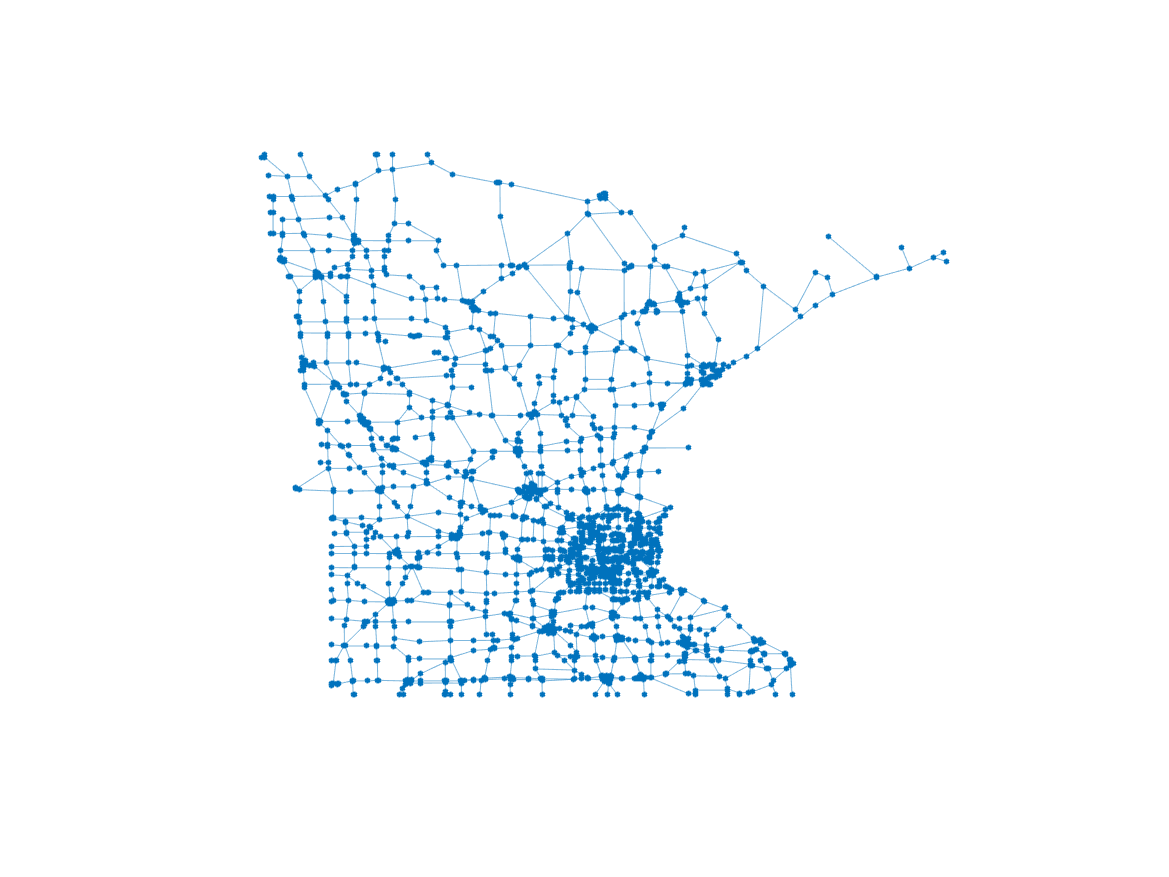
\includegraphics[scale=0.8]{Figure/minnesota}
	\caption{Grafico della rete stradale del Minnesota.}
	\label{fig::minnesota}
\end{figure}
\begin{figure}[ht]
\centering
\subfloat[][$\gamma=0.10$]
{\resizebox{0.45\textwidth}{!}{% This file was created by matlab2tikz.
%
%The latest updates can be retrieved from
%  http://www.mathworks.com/matlabcentral/fileexchange/22022-matlab2tikz-matlab2tikz
%where you can also make suggestions and rate matlab2tikz.
%
\definecolor{mycolor1}{rgb}{0.00000,0.44700,0.74100}%
\definecolor{mycolor2}{rgb}{0.85000,0.32500,0.09800}%
%
\begin{tikzpicture}

\begin{axis}[%
width=0.39\columnwidth,
height=1.7in,
at={(1.011in,0.642in)},
scale only axis,
xmin=0,
xmax=1,
xlabel style={font=\color{white!15!black}},
xlabel={$\tau$},
ymin=0,
ymax=16000,
axis background/.style={fill=white},
legend columns=2,
legend pos=north west,
legend style={legend cell align=left, align=left, draw=none,fill=none}
]
\addplot [color=mycolor1, line width=2.0pt]
  table[row sep=crcr]{%
0	693\\
0.00252525252525253	693\\
0.00505050505050505	693\\
0.00757575757575758	693\\
0.0101010101010101	693\\
0.0126262626262626	693\\
0.0151515151515152	693\\
0.0176767676767677	693\\
0.0202020202020202	697\\
0.0227272727272727	701\\
0.0252525252525253	709\\
0.0277777777777778	717\\
0.0303030303030303	725\\
0.0328282828282828	733\\
0.0353535353535354	741\\
0.0378787878787879	749\\
0.0404040404040404	757\\
0.0429292929292929	765\\
0.0454545454545455	773\\
0.047979797979798	781\\
0.0505050505050505	785\\
0.053030303030303	793\\
0.0555555555555556	801\\
0.0580808080808081	809\\
0.0606060606060606	813\\
0.0631313131313131	821\\
0.0656565656565657	829\\
0.0681818181818182	833\\
0.0707070707070707	841\\
0.0732323232323232	845\\
0.0757575757575758	853\\
0.0782828282828283	861\\
0.0808080808080808	869\\
0.0833333333333333	881\\
0.0858585858585859	897\\
0.0883838383838384	913\\
0.0909090909090909	933\\
0.0934343434343434	957\\
0.095959595959596	981\\
0.0984848484848485	1001\\
0.101010101010101	1025\\
0.103535353535354	1049\\
0.106060606060606	1077\\
0.108585858585859	1101\\
0.111111111111111	1125\\
0.113636363636364	1153\\
0.116161616161616	1177\\
0.118686868686869	1205\\
0.121212121212121	1233\\
0.123737373737374	1261\\
0.126262626262626	1289\\
0.128787878787879	1317\\
0.131313131313131	1349\\
0.133838383838384	1377\\
0.136363636363636	1409\\
0.138888888888889	1441\\
0.141414141414141	1473\\
0.143939393939394	1505\\
0.146464646464646	1537\\
0.148989898989899	1569\\
0.151515151515152	1605\\
0.154040404040404	1637\\
0.156565656565657	1669\\
0.159090909090909	1701\\
0.161616161616162	1733\\
0.164141414141414	1765\\
0.166666666666667	1797\\
0.169191919191919	1829\\
0.171717171717172	1861\\
0.174242424242424	1897\\
0.176767676767677	1929\\
0.179292929292929	1961\\
0.181818181818182	1993\\
0.184343434343434	2029\\
0.186868686868687	2065\\
0.189393939393939	2097\\
0.191919191919192	2133\\
0.194444444444444	2165\\
0.196969696969697	2201\\
0.19949494949495	2237\\
0.202020202020202	2273\\
0.204545454545455	2309\\
0.207070707070707	2345\\
0.20959595959596	2381\\
0.212121212121212	2417\\
0.214646464646465	2453\\
0.217171717171717	2493\\
0.21969696969697	2533\\
0.222222222222222	2569\\
0.224747474747475	2609\\
0.227272727272727	2645\\
0.22979797979798	2685\\
0.232323232323232	2721\\
0.234848484848485	2757\\
0.237373737373737	2793\\
0.23989898989899	2829\\
0.242424242424242	2869\\
0.244949494949495	2905\\
0.247474747474747	2945\\
0.25	2981\\
0.25	2981\\
0.252525252525253	3017\\
0.255050505050505	3053\\
0.257575757575758	3093\\
0.26010101010101	3133\\
0.262626262626263	3173\\
0.265151515151515	3213\\
0.267676767676768	3253\\
0.27020202020202	3293\\
0.272727272727273	3333\\
0.275252525252525	3373\\
0.277777777777778	3413\\
0.28030303030303	3449\\
0.282828282828283	3489\\
0.285353535353535	3529\\
0.287878787878788	3569\\
0.29040404040404	3609\\
0.292929292929293	3649\\
0.295454545454545	3689\\
0.297979797979798	3729\\
0.30050505050505	3769\\
0.303030303030303	3809\\
0.305555555555556	3849\\
0.308080808080808	3889\\
0.310606060606061	3929\\
0.313131313131313	3969\\
0.315656565656566	4009\\
0.318181818181818	4045\\
0.320707070707071	4085\\
0.323232323232323	4125\\
0.325757575757576	4165\\
0.328282828282828	4205\\
0.330808080808081	4245\\
0.333333333333333	4281\\
0.335858585858586	4321\\
0.338383838383838	4361\\
0.340909090909091	4397\\
0.343434343434343	4437\\
0.345959595959596	4481\\
0.348484848484849	4525\\
0.351010101010101	4565\\
0.353535353535354	4609\\
0.356060606060606	4649\\
0.358585858585859	4689\\
0.361111111111111	4729\\
0.363636363636364	4769\\
0.366161616161616	4809\\
0.368686868686869	4849\\
0.371212121212121	4889\\
0.373737373737374	4929\\
0.376262626262626	4973\\
0.378787878787879	5013\\
0.381313131313131	5053\\
0.383838383838384	5093\\
0.386363636363636	5137\\
0.388888888888889	5177\\
0.391414141414141	5217\\
0.393939393939394	5257\\
0.396464646464646	5297\\
0.398989898989899	5341\\
0.401515151515151	5381\\
0.404040404040404	5421\\
0.406565656565657	5461\\
0.409090909090909	5501\\
0.411616161616162	5541\\
0.414141414141414	5581\\
0.416666666666667	5621\\
0.419191919191919	5661\\
0.421717171717172	5705\\
0.424242424242424	5745\\
0.426767676767677	5785\\
0.429292929292929	5825\\
0.431818181818182	5869\\
0.434343434343434	5909\\
0.436868686868687	5949\\
0.439393939393939	5993\\
0.441919191919192	6037\\
0.444444444444444	6077\\
0.446969696969697	6121\\
0.44949494949495	6161\\
0.452020202020202	6205\\
0.454545454545455	6249\\
0.457070707070707	6289\\
0.45959595959596	6333\\
0.462121212121212	6373\\
0.464646464646465	6413\\
0.467171717171717	6453\\
0.46969696969697	6497\\
0.472222222222222	6537\\
0.474747474747475	6581\\
0.477272727272727	6625\\
0.47979797979798	6669\\
0.482323232323232	6713\\
0.484848484848485	6753\\
0.487373737373737	6797\\
0.48989898989899	6841\\
0.492424242424242	6885\\
0.494949494949495	6929\\
0.497474747474748	6977\\
0.5	7021\\
0.5	7021\\
0.502525252525252	7061\\
0.505050505050505	7105\\
0.507575757575758	7149\\
0.51010101010101	7189\\
0.512626262626263	7233\\
0.515151515151515	7273\\
0.517676767676768	7317\\
0.52020202020202	7361\\
0.522727272727273	7401\\
0.525252525252525	7445\\
0.527777777777778	7485\\
0.53030303030303	7529\\
0.532828282828283	7569\\
0.535353535353535	7613\\
0.537878787878788	7653\\
0.54040404040404	7697\\
0.542929292929293	7741\\
0.545454545454545	7781\\
0.547979797979798	7825\\
0.55050505050505	7865\\
0.553030303030303	7909\\
0.555555555555556	7953\\
0.558080808080808	7997\\
0.560606060606061	8041\\
0.563131313131313	8085\\
0.565656565656566	8129\\
0.568181818181818	8169\\
0.570707070707071	8213\\
0.573232323232323	8253\\
0.575757575757576	8293\\
0.578282828282828	8337\\
0.580808080808081	8377\\
0.583333333333333	8417\\
0.585858585858586	8457\\
0.588383838383838	8501\\
0.590909090909091	8541\\
0.593434343434343	8585\\
0.595959595959596	8629\\
0.598484848484849	8669\\
0.601010101010101	8713\\
0.603535353535354	8757\\
0.606060606060606	8801\\
0.608585858585859	8845\\
0.611111111111111	8885\\
0.613636363636364	8929\\
0.616161616161616	8977\\
0.618686868686869	9021\\
0.621212121212121	9065\\
0.623737373737374	9109\\
0.626262626262626	9153\\
0.628787878787879	9197\\
0.631313131313131	9241\\
0.633838383838384	9285\\
0.636363636363636	9329\\
0.638888888888889	9369\\
0.641414141414141	9413\\
0.643939393939394	9457\\
0.646464646464646	9501\\
0.648989898989899	9545\\
0.651515151515151	9589\\
0.654040404040404	9633\\
0.656565656565657	9677\\
0.659090909090909	9721\\
0.661616161616162	9765\\
0.664141414141414	9809\\
0.666666666666667	9853\\
0.669191919191919	9897\\
0.671717171717172	9945\\
0.674242424242424	9989\\
0.676767676767677	10037\\
0.679292929292929	10081\\
0.681818181818182	10125\\
0.684343434343434	10169\\
0.686868686868687	10213\\
0.689393939393939	10257\\
0.691919191919192	10297\\
0.694444444444444	10341\\
0.696969696969697	10381\\
0.69949494949495	10425\\
0.702020202020202	10469\\
0.704545454545455	10509\\
0.707070707070707	10553\\
0.70959595959596	10597\\
0.712121212121212	10641\\
0.714646464646465	10681\\
0.717171717171717	10725\\
0.71969696969697	10773\\
0.722222222222222	10817\\
0.724747474747475	10861\\
0.727272727272727	10905\\
0.72979797979798	10953\\
0.732323232323232	10997\\
0.734848484848485	11041\\
0.737373737373737	11085\\
0.73989898989899	11133\\
0.742424242424242	11177\\
0.744949494949495	11221\\
0.747474747474748	11265\\
0.75	11309\\
0.75	11309\\
0.752525252525252	11353\\
0.755050505050505	11397\\
0.757575757575758	11441\\
0.76010101010101	11481\\
0.762626262626263	11525\\
0.765151515151515	11565\\
0.767676767676768	11613\\
0.77020202020202	11657\\
0.772727272727273	11705\\
0.775252525252525	11749\\
0.777777777777778	11797\\
0.78030303030303	11841\\
0.782828282828283	11889\\
0.785353535353535	11933\\
0.787878787878788	11977\\
0.79040404040404	12021\\
0.792929292929293	12065\\
0.795454545454545	12109\\
0.797979797979798	12153\\
0.80050505050505	12193\\
0.803030303030303	12233\\
0.805555555555556	12277\\
0.808080808080808	12317\\
0.810606060606061	12357\\
0.813131313131313	12401\\
0.815656565656566	12441\\
0.818181818181818	12485\\
0.820707070707071	12529\\
0.823232323232323	12577\\
0.825757575757576	12621\\
0.828282828282828	12669\\
0.830808080808081	12713\\
0.833333333333333	12761\\
0.835858585858586	12805\\
0.838383838383838	12853\\
0.840909090909091	12897\\
0.843434343434343	12941\\
0.845959595959596	12985\\
0.848484848484849	13029\\
0.851010101010101	13073\\
0.853535353535354	13117\\
0.856060606060606	13161\\
0.858585858585859	13201\\
0.861111111111111	13241\\
0.863636363636364	13281\\
0.866161616161616	13321\\
0.868686868686869	13361\\
0.871212121212121	13397\\
0.873737373737374	13437\\
0.876262626262626	13477\\
0.878787878787879	13517\\
0.881313131313131	13557\\
0.883838383838384	13601\\
0.886363636363636	13645\\
0.888888888888889	13693\\
0.891414141414141	13737\\
0.893939393939394	13781\\
0.896464646464646	13825\\
0.898989898989899	13873\\
0.901515151515151	13917\\
0.904040404040404	13957\\
0.906565656565657	14001\\
0.909090909090909	14041\\
0.911616161616162	14081\\
0.914141414141414	14121\\
0.916666666666667	14161\\
0.919191919191919	14197\\
0.921717171717172	14237\\
0.924242424242424	14277\\
0.926767676767677	14317\\
0.929292929292929	14357\\
0.931818181818182	14401\\
0.934343434343434	14445\\
0.936868686868687	14489\\
0.939393939393939	14533\\
0.941919191919192	14577\\
0.944444444444444	14617\\
0.946969696969697	14661\\
0.94949494949495	14701\\
0.952020202020202	14741\\
0.954545454545455	14781\\
0.957070707070707	14821\\
0.95959595959596	14861\\
0.962121212121212	14897\\
0.964646464646465	14937\\
0.967171717171717	14973\\
0.96969696969697	15013\\
0.972222222222222	15049\\
0.974747474747475	15085\\
0.977272727272727	15125\\
0.97979797979798	15165\\
0.982323232323232	15205\\
0.984848484848485	15245\\
0.987373737373737	15285\\
0.98989898989899	15325\\
0.992424242424242	15365\\
0.994949494949495	15405\\
0.997474747474748	15445\\
1	15485\\
};
\addlegendentry{ode45}

\addplot [color=mycolor2, line width=2.0pt]
  table[row sep=crcr]{%
0	253\\
0.00252525252525253	253\\
0.00505050505050505	253\\
0.00757575757575758	253\\
0.0101010101010101	253\\
0.0126262626262626	255\\
0.0151515151515152	259\\
0.0176767676767677	265\\
0.0202020202020202	271\\
0.0227272727272727	277\\
0.0252525252525253	282\\
0.0277777777777778	288\\
0.0303030303030303	295\\
0.0328282828282828	300\\
0.0353535353535354	305\\
0.0378787878787879	311\\
0.0404040404040404	312\\
0.0429292929292929	320\\
0.0454545454545455	324\\
0.047979797979798	329\\
0.0505050505050505	333\\
0.053030303030303	338\\
0.0555555555555556	342\\
0.0580808080808081	346\\
0.0606060606060606	350\\
0.0631313131313131	354\\
0.0656565656565657	358\\
0.0681818181818182	361\\
0.0707070707070707	365\\
0.0732323232323232	369\\
0.0757575757575758	373\\
0.0782828282828283	380\\
0.0808080808080808	387\\
0.0833333333333333	395\\
0.0858585858585859	403\\
0.0883838383838384	415\\
0.0909090909090909	424\\
0.0934343434343434	434\\
0.095959595959596	443\\
0.0984848484848485	454\\
0.101010101010101	464\\
0.103535353535354	475\\
0.106060606060606	486\\
0.108585858585859	497\\
0.111111111111111	509\\
0.113636363636364	522\\
0.116161616161616	529\\
0.118686868686869	543\\
0.121212121212121	557\\
0.123737373737374	574\\
0.126262626262626	588\\
0.128787878787879	597\\
0.131313131313131	611\\
0.133838383838384	625\\
0.136363636363636	638\\
0.138888888888889	652\\
0.141414141414141	665\\
0.143939393939394	679\\
0.146464646464646	692\\
0.148989898989899	706\\
0.151515151515152	719\\
0.154040404040404	732\\
0.156565656565657	745\\
0.159090909090909	759\\
0.161616161616162	773\\
0.164141414141414	786\\
0.166666666666667	800\\
0.169191919191919	813\\
0.171717171717172	826\\
0.174242424242424	840\\
0.176767676767677	853\\
0.179292929292929	866\\
0.181818181818182	880\\
0.184343434343434	894\\
0.186868686868687	908\\
0.189393939393939	922\\
0.191919191919192	935\\
0.194444444444444	949\\
0.196969696969697	962\\
0.19949494949495	976\\
0.202020202020202	989\\
0.204545454545455	1002\\
0.207070707070707	1017\\
0.20959595959596	1031\\
0.212121212121212	1044\\
0.214646464646465	1059\\
0.217171717171717	1072\\
0.21969696969697	1088\\
0.222222222222222	1099\\
0.224747474747475	1115\\
0.227272727272727	1128\\
0.22979797979798	1145\\
0.232323232323232	1157\\
0.234848484848485	1169\\
0.237373737373737	1186\\
0.23989898989899	1204\\
0.242424242424242	1219\\
0.244949494949495	1236\\
0.247474747474747	1252\\
0.25	1272\\
0.25	1272\\
0.252525252525253	1289\\
0.255050505050505	1302\\
0.257575757575758	1319\\
0.26010101010101	1335\\
0.262626262626263	1351\\
0.265151515151515	1366\\
0.267676767676768	1380\\
0.27020202020202	1395\\
0.272727272727273	1409\\
0.275252525252525	1424\\
0.277777777777778	1439\\
0.28030303030303	1453\\
0.282828282828283	1467\\
0.285353535353535	1481\\
0.287878787878788	1496\\
0.29040404040404	1511\\
0.292929292929293	1526\\
0.295454545454545	1541\\
0.297979797979798	1555\\
0.30050505050505	1570\\
0.303030303030303	1585\\
0.305555555555556	1600\\
0.308080808080808	1614\\
0.310606060606061	1629\\
0.313131313131313	1644\\
0.315656565656566	1660\\
0.318181818181818	1675\\
0.320707070707071	1693\\
0.323232323232323	1711\\
0.325757575757576	1729\\
0.328282828282828	1745\\
0.330808080808081	1762\\
0.333333333333333	1779\\
0.335858585858586	1794\\
0.338383838383838	1810\\
0.340909090909091	1825\\
0.343434343434343	1844\\
0.345959595959596	1860\\
0.348484848484849	1876\\
0.351010101010101	1890\\
0.353535353535354	1907\\
0.356060606060606	1922\\
0.358585858585859	1938\\
0.361111111111111	1953\\
0.363636363636364	1970\\
0.366161616161616	1988\\
0.368686868686869	2005\\
0.371212121212121	2021\\
0.373737373737374	2033\\
0.376262626262626	2051\\
0.378787878787879	2067\\
0.381313131313131	2083\\
0.383838383838384	2099\\
0.386363636363636	2114\\
0.388888888888889	2130\\
0.391414141414141	2144\\
0.393939393939394	2160\\
0.396464646464646	2176\\
0.398989898989899	2194\\
0.401515151515151	2207\\
0.404040404040404	2222\\
0.406565656565657	2239\\
0.409090909090909	2255\\
0.411616161616162	2271\\
0.414141414141414	2287\\
0.416666666666667	2304\\
0.419191919191919	2317\\
0.421717171717172	2332\\
0.424242424242424	2349\\
0.426767676767677	2365\\
0.429292929292929	2381\\
0.431818181818182	2398\\
0.434343434343434	2410\\
0.436868686868687	2424\\
0.439393939393939	2438\\
0.441919191919192	2453\\
0.444444444444444	2471\\
0.446969696969697	2493\\
0.44949494949495	2519\\
0.452020202020202	2532\\
0.454545454545455	2542\\
0.457070707070707	2559\\
0.45959595959596	2577\\
0.462121212121212	2596\\
0.464646464646465	2613\\
0.467171717171717	2628\\
0.46969696969697	2655\\
0.472222222222222	2670\\
0.474747474747475	2682\\
0.477272727272727	2698\\
0.47979797979798	2715\\
0.482323232323232	2732\\
0.484848484848485	2745\\
0.487373737373737	2757\\
0.48989898989899	2776\\
0.492424242424242	2792\\
0.494949494949495	2827\\
0.497474747474748	2844\\
0.5	2848\\
0.5	2848\\
0.502525252525252	2865\\
0.505050505050505	2881\\
0.507575757575758	2896\\
0.51010101010101	2917\\
0.512626262626263	2933\\
0.515151515151515	2946\\
0.517676767676768	2964\\
0.52020202020202	2979\\
0.522727272727273	2997\\
0.525252525252525	3014\\
0.527777777777778	3028\\
0.53030303030303	3048\\
0.532828282828283	3063\\
0.535353535353535	3081\\
0.537878787878788	3097\\
0.54040404040404	3114\\
0.542929292929293	3126\\
0.545454545454545	3143\\
0.547979797979798	3159\\
0.55050505050505	3175\\
0.553030303030303	3193\\
0.555555555555556	3211\\
0.558080808080808	3227\\
0.560606060606061	3244\\
0.563131313131313	3262\\
0.565656565656566	3269\\
0.568181818181818	3283\\
0.570707070707071	3301\\
0.573232323232323	3328\\
0.575757575757576	3340\\
0.578282828282828	3357\\
0.580808080808081	3374\\
0.583333333333333	3391\\
0.585858585858586	3418\\
0.588383838383838	3430\\
0.590909090909091	3443\\
0.593434343434343	3460\\
0.595959595959596	3474\\
0.598484848484849	3495\\
0.601010101010101	3512\\
0.603535353535354	3529\\
0.606060606060606	3540\\
0.608585858585859	3561\\
0.611111111111111	3573\\
0.613636363636364	3595\\
0.616161616161616	3611\\
0.618686868686869	3627\\
0.621212121212121	3643\\
0.623737373737374	3659\\
0.626262626262626	3680\\
0.628787878787879	3703\\
0.631313131313131	3719\\
0.633838383838384	3741\\
0.636363636363636	3755\\
0.638888888888889	3771\\
0.641414141414141	3790\\
0.643939393939394	3812\\
0.646464646464646	3825\\
0.648989898989899	3843\\
0.651515151515151	3864\\
0.654040404040404	3883\\
0.656565656565657	3901\\
0.659090909090909	3918\\
0.661616161616162	3932\\
0.664141414141414	3951\\
0.666666666666667	3967\\
0.669191919191919	3985\\
0.671717171717172	4004\\
0.674242424242424	4024\\
0.676767676767677	4043\\
0.679292929292929	4062\\
0.681818181818182	4081\\
0.684343434343434	4099\\
0.686868686868687	4112\\
0.689393939393939	4132\\
0.691919191919192	4144\\
0.694444444444444	4151\\
0.696969696969697	4168\\
0.69949494949495	4198\\
0.702020202020202	4210\\
0.704545454545455	4225\\
0.707070707070707	4239\\
0.70959595959596	4254\\
0.712121212121212	4271\\
0.714646464646465	4286\\
0.717171717171717	4303\\
0.71969696969697	4317\\
0.722222222222222	4337\\
0.724747474747475	4357\\
0.727272727272727	4374\\
0.72979797979798	4392\\
0.732323232323232	4412\\
0.734848484848485	4431\\
0.737373737373737	4447\\
0.73989898989899	4467\\
0.742424242424242	4487\\
0.744949494949495	4506\\
0.747474747474748	4523\\
0.75	4542\\
0.75	4542\\
0.752525252525252	4560\\
0.755050505050505	4576\\
0.757575757575758	4599\\
0.76010101010101	4625\\
0.762626262626263	4646\\
0.765151515151515	4675\\
0.767676767676768	4711\\
0.77020202020202	4754\\
0.772727272727273	4809\\
0.775252525252525	4875\\
0.777777777777778	4968\\
0.78030303030303	5101\\
0.782828282828283	5423\\
0.785353535353535	10728\\
0.787878787878788	10726\\
0.79040404040404	10725\\
0.792929292929293	10722\\
0.795454545454545	10719\\
0.797979797979798	10718\\
0.80050505050505	10716\\
0.803030303030303	10711\\
0.805555555555556	10712\\
0.808080808080808	10710\\
0.810606060606061	10708\\
0.813131313131313	10706\\
0.815656565656566	10706\\
0.818181818181818	10704\\
0.820707070707071	10703\\
0.823232323232323	10700\\
0.825757575757576	10700\\
0.828282828282828	10698\\
0.830808080808081	10697\\
0.833333333333333	10695\\
0.835858585858586	10696\\
0.838383838383838	10694\\
0.840909090909091	10693\\
0.843434343434343	10691\\
0.845959595959596	10693\\
0.848484848484849	10687\\
0.851010101010101	10690\\
0.853535353535354	10685\\
0.856060606060606	10686\\
0.858585858585859	10685\\
0.861111111111111	10685\\
0.863636363636364	10681\\
0.866161616161616	10684\\
0.868686868686869	10678\\
0.871212121212121	5339\\
0.873737373737374	5357\\
0.876262626262626	5376\\
0.878787878787879	5391\\
0.881313131313131	5401\\
0.883838383838384	5423\\
0.886363636363636	10925\\
0.888888888888889	10964\\
0.891414141414141	10950\\
0.893939393939394	10966\\
0.896464646464646	10953\\
0.898989898989899	10972\\
0.901515151515151	10956\\
0.904040404040404	11030\\
0.906565656565657	10961\\
0.909090909090909	11042\\
0.911616161616162	11019\\
0.914141414141414	10951\\
0.916666666666667	11032\\
0.919191919191919	11010\\
0.921717171717172	10950\\
0.924242424242424	11021\\
0.926767676767677	10998\\
0.929292929292929	10980\\
0.931818181818182	10931\\
0.934343434343434	10974\\
0.936868686868687	10977\\
0.939393939393939	10928\\
0.941919191919192	10915\\
0.944444444444444	10952\\
0.946969696969697	10940\\
0.94949494949495	10898\\
0.952020202020202	10940\\
0.954545454545455	10931\\
0.957070707070707	10920\\
0.95959595959596	10884\\
0.962121212121212	10879\\
0.964646464646465	10906\\
0.967171717171717	10894\\
0.96969696969697	10886\\
0.972222222222222	10870\\
0.974747474747475	10866\\
0.977272727272727	10884\\
0.97979797979798	10879\\
0.982323232323232	10875\\
0.984848484848485	10849\\
0.987373737373737	10845\\
0.98989898989899	10875\\
0.992424242424242	10872\\
0.994949494949495	10866\\
0.997474747474748	10842\\
1	10845\\
};
\addlegendentry{ode15s}
\end{axis}
\end{tikzpicture}%}}
 \quad 
\subfloat[][$\gamma=0.30$]
{\resizebox{0.45\textwidth}{!}{ % This file was created by matlab2tikz.
%
%The latest updates can be retrieved from
%  http://www.mathworks.com/matlabcentral/fileexchange/22022-matlab2tikz-matlab2tikz
%where you can also make suggestions and rate matlab2tikz.
%
\definecolor{mycolor1}{rgb}{0.00000,0.44700,0.74100}%
\definecolor{mycolor2}{rgb}{0.85000,0.32500,0.09800}%
%
\begin{tikzpicture}

\begin{axis}[%
width=6.028in,
height=4.754in,
at={(1.011in,0.642in)},
scale only axis,
xmin=0,
xmax=1,
xlabel style={font=\color{white!15!black}},
xlabel={$\tau$},
ymin=0,
ymax=14000,
ylabel style={font=\color{white!15!black}},
ylabel={iterazioni},
axis background/.style={fill=white},
legend style={legend cell align=left, align=left, draw=white!15!black}
]
\addplot [color=mycolor1, line width=2.0pt]
  table[row sep=crcr]{%
0	1281\\
0.00252525252525253	1281\\
0.00505050505050505	1281\\
0.00757575757575758	1281\\
0.0101010101010101	1281\\
0.0126262626262626	1281\\
0.0151515151515152	1281\\
0.0176767676767677	1281\\
0.0202020202020202	1281\\
0.0227272727272727	1281\\
0.0252525252525253	1281\\
0.0277777777777778	1281\\
0.0303030303030303	1281\\
0.0328282828282828	1281\\
0.0353535353535354	1281\\
0.0378787878787879	1281\\
0.0404040404040404	1281\\
0.0429292929292929	1281\\
0.0454545454545455	1281\\
0.047979797979798	1281\\
0.0505050505050505	1281\\
0.053030303030303	1281\\
0.0555555555555556	1281\\
0.0580808080808081	1285\\
0.0606060606060606	1285\\
0.0631313131313131	1289\\
0.0656565656565657	1289\\
0.0681818181818182	1293\\
0.0707070707070707	1293\\
0.0732323232323232	1297\\
0.0757575757575758	1297\\
0.0782828282828283	1301\\
0.0808080808080808	1305\\
0.0833333333333333	1305\\
0.0858585858585859	1309\\
0.0883838383838384	1309\\
0.0909090909090909	1313\\
0.0934343434343434	1317\\
0.095959595959596	1317\\
0.0984848484848485	1321\\
0.101010101010101	1325\\
0.103535353535354	1325\\
0.106060606060606	1329\\
0.108585858585859	1333\\
0.111111111111111	1333\\
0.113636363636364	1337\\
0.116161616161616	1341\\
0.118686868686869	1341\\
0.121212121212121	1345\\
0.123737373737374	1349\\
0.126262626262626	1349\\
0.128787878787879	1353\\
0.131313131313131	1357\\
0.133838383838384	1357\\
0.136363636363636	1361\\
0.138888888888889	1365\\
0.141414141414141	1365\\
0.143939393939394	1369\\
0.146464646464646	1373\\
0.148989898989899	1381\\
0.151515151515152	1389\\
0.154040404040404	1397\\
0.156565656565657	1405\\
0.159090909090909	1413\\
0.161616161616162	1425\\
0.164141414141414	1433\\
0.166666666666667	1445\\
0.169191919191919	1457\\
0.171717171717172	1473\\
0.174242424242424	1485\\
0.176767676767677	1497\\
0.179292929292929	1513\\
0.181818181818182	1529\\
0.184343434343434	1541\\
0.186868686868687	1557\\
0.189393939393939	1573\\
0.191919191919192	1589\\
0.194444444444444	1605\\
0.196969696969697	1621\\
0.19949494949495	1637\\
0.202020202020202	1653\\
0.204545454545455	1673\\
0.207070707070707	1689\\
0.20959595959596	1709\\
0.212121212121212	1729\\
0.214646464646465	1749\\
0.217171717171717	1773\\
0.21969696969697	1793\\
0.222222222222222	1817\\
0.224747474747475	1837\\
0.227272727272727	1861\\
0.22979797979798	1885\\
0.232323232323232	1909\\
0.234848484848485	1933\\
0.237373737373737	1957\\
0.23989898989899	1981\\
0.242424242424242	2005\\
0.244949494949495	2029\\
0.247474747474747	2057\\
0.25	2081\\
0.25	2081\\
0.252525252525253	2109\\
0.255050505050505	2137\\
0.257575757575758	2169\\
0.26010101010101	2197\\
0.262626262626263	2229\\
0.265151515151515	2261\\
0.267676767676768	2293\\
0.27020202020202	2321\\
0.272727272727273	2353\\
0.275252525252525	2381\\
0.277777777777778	2413\\
0.28030303030303	2441\\
0.282828282828283	2469\\
0.285353535353535	2501\\
0.287878787878788	2529\\
0.29040404040404	2561\\
0.292929292929293	2589\\
0.295454545454545	2621\\
0.297979797979798	2653\\
0.30050505050505	2681\\
0.303030303030303	2713\\
0.305555555555556	2741\\
0.308080808080808	2773\\
0.310606060606061	2805\\
0.313131313131313	2837\\
0.315656565656566	2865\\
0.318181818181818	2897\\
0.320707070707071	2929\\
0.323232323232323	2961\\
0.325757575757576	2993\\
0.328282828282828	3021\\
0.330808080808081	3053\\
0.333333333333333	3085\\
0.335858585858586	3117\\
0.338383838383838	3153\\
0.340909090909091	3185\\
0.343434343434343	3221\\
0.345959595959596	3257\\
0.348484848484849	3293\\
0.351010101010101	3329\\
0.353535353535354	3365\\
0.356060606060606	3401\\
0.358585858585859	3433\\
0.361111111111111	3465\\
0.363636363636364	3501\\
0.366161616161616	3533\\
0.368686868686869	3569\\
0.371212121212121	3601\\
0.373737373737374	3637\\
0.376262626262626	3673\\
0.378787878787879	3705\\
0.381313131313131	3741\\
0.383838383838384	3773\\
0.386363636363636	3809\\
0.388888888888889	3841\\
0.391414141414141	3873\\
0.393939393939394	3909\\
0.396464646464646	3941\\
0.398989898989899	3977\\
0.401515151515151	4009\\
0.404040404040404	4045\\
0.406565656565657	4077\\
0.409090909090909	4113\\
0.411616161616162	4145\\
0.414141414141414	4181\\
0.416666666666667	4213\\
0.419191919191919	4249\\
0.421717171717172	4285\\
0.424242424242424	4317\\
0.426767676767677	4353\\
0.429292929292929	4389\\
0.431818181818182	4425\\
0.434343434343434	4461\\
0.436868686868687	4497\\
0.439393939393939	4533\\
0.441919191919192	4569\\
0.444444444444444	4605\\
0.446969696969697	4641\\
0.44949494949495	4677\\
0.452020202020202	4709\\
0.454545454545455	4745\\
0.457070707070707	4781\\
0.45959595959596	4813\\
0.462121212121212	4849\\
0.464646464646465	4889\\
0.467171717171717	4925\\
0.46969696969697	4965\\
0.472222222222222	5001\\
0.474747474747475	5041\\
0.477272727272727	5081\\
0.47979797979798	5121\\
0.482323232323232	5157\\
0.484848484848485	5197\\
0.487373737373737	5237\\
0.48989898989899	5277\\
0.492424242424242	5317\\
0.494949494949495	5361\\
0.497474747474748	5401\\
0.5	5441\\
0.5	5441\\
0.502525252525252	5481\\
0.505050505050505	5521\\
0.507575757575758	5557\\
0.51010101010101	5593\\
0.512626262626263	5633\\
0.515151515151515	5669\\
0.517676767676768	5709\\
0.52020202020202	5745\\
0.522727272727273	5785\\
0.525252525252525	5821\\
0.527777777777778	5861\\
0.53030303030303	5897\\
0.532828282828283	5937\\
0.535353535353535	5973\\
0.537878787878788	6013\\
0.54040404040404	6053\\
0.542929292929293	6093\\
0.545454545454545	6129\\
0.547979797979798	6169\\
0.55050505050505	6209\\
0.553030303030303	6249\\
0.555555555555556	6289\\
0.558080808080808	6329\\
0.560606060606061	6369\\
0.563131313131313	6409\\
0.565656565656566	6445\\
0.568181818181818	6485\\
0.570707070707071	6521\\
0.573232323232323	6557\\
0.575757575757576	6597\\
0.578282828282828	6633\\
0.580808080808081	6669\\
0.583333333333333	6705\\
0.585858585858586	6745\\
0.588383838383838	6781\\
0.590909090909091	6821\\
0.593434343434343	6857\\
0.595959595959596	6893\\
0.598484848484849	6933\\
0.601010101010101	6973\\
0.603535353535354	7013\\
0.606060606060606	7049\\
0.608585858585859	7089\\
0.611111111111111	7129\\
0.613636363636364	7169\\
0.616161616161616	7209\\
0.618686868686869	7249\\
0.621212121212121	7289\\
0.623737373737374	7329\\
0.626262626262626	7373\\
0.628787878787879	7413\\
0.631313131313131	7453\\
0.633838383838384	7493\\
0.636363636363636	7533\\
0.638888888888889	7573\\
0.641414141414141	7613\\
0.643939393939394	7649\\
0.646464646464646	7689\\
0.648989898989899	7729\\
0.651515151515151	7769\\
0.654040404040404	7813\\
0.656565656565657	7853\\
0.659090909090909	7893\\
0.661616161616162	7933\\
0.664141414141414	7973\\
0.666666666666667	8017\\
0.669191919191919	8061\\
0.671717171717172	8105\\
0.674242424242424	8149\\
0.676767676767677	8193\\
0.679292929292929	8237\\
0.681818181818182	8277\\
0.684343434343434	8321\\
0.686868686868687	8361\\
0.689393939393939	8401\\
0.691919191919192	8441\\
0.694444444444444	8481\\
0.696969696969697	8521\\
0.69949494949495	8561\\
0.702020202020202	8605\\
0.704545454545455	8645\\
0.707070707070707	8685\\
0.70959595959596	8725\\
0.712121212121212	8769\\
0.714646464646465	8809\\
0.717171717171717	8853\\
0.71969696969697	8897\\
0.722222222222222	8941\\
0.724747474747475	8981\\
0.727272727272727	9025\\
0.72979797979798	9069\\
0.732323232323232	9113\\
0.734848484848485	9157\\
0.737373737373737	9197\\
0.73989898989899	9241\\
0.742424242424242	9285\\
0.744949494949495	9325\\
0.747474747474748	9369\\
0.75	9409\\
0.75	9409\\
0.752525252525252	9453\\
0.755050505050505	9493\\
0.757575757575758	9533\\
0.76010101010101	9573\\
0.762626262626263	9617\\
0.765151515151515	9657\\
0.767676767676768	9701\\
0.77020202020202	9745\\
0.772727272727273	9785\\
0.775252525252525	9829\\
0.777777777777778	9873\\
0.78030303030303	9913\\
0.782828282828283	9957\\
0.785353535353535	10001\\
0.787878787878788	10041\\
0.79040404040404	10085\\
0.792929292929293	10125\\
0.795454545454545	10169\\
0.797979797979798	10209\\
0.80050505050505	10249\\
0.803030303030303	10293\\
0.805555555555556	10333\\
0.808080808080808	10373\\
0.810606060606061	10413\\
0.813131313131313	10457\\
0.815656565656566	10497\\
0.818181818181818	10541\\
0.820707070707071	10589\\
0.823232323232323	10633\\
0.825757575757576	10673\\
0.828282828282828	10721\\
0.830808080808081	10765\\
0.833333333333333	10809\\
0.835858585858586	10857\\
0.838383838383838	10901\\
0.840909090909091	10945\\
0.843434343434343	10989\\
0.845959595959596	11029\\
0.848484848484849	11073\\
0.851010101010101	11113\\
0.853535353535354	11153\\
0.856060606060606	11193\\
0.858585858585859	11233\\
0.861111111111111	11273\\
0.863636363636364	11313\\
0.866161616161616	11357\\
0.868686868686869	11401\\
0.871212121212121	11441\\
0.873737373737374	11489\\
0.876262626262626	11533\\
0.878787878787879	11577\\
0.881313131313131	11621\\
0.883838383838384	11665\\
0.886363636363636	11709\\
0.888888888888889	11749\\
0.891414141414141	11793\\
0.893939393939394	11837\\
0.896464646464646	11881\\
0.898989898989899	11925\\
0.901515151515151	11969\\
0.904040404040404	12009\\
0.906565656565657	12049\\
0.909090909090909	12085\\
0.911616161616162	12125\\
0.914141414141414	12161\\
0.916666666666667	12197\\
0.919191919191919	12237\\
0.921717171717172	12273\\
0.924242424242424	12313\\
0.926767676767677	12349\\
0.929292929292929	12393\\
0.931818181818182	12433\\
0.934343434343434	12477\\
0.936868686868687	12521\\
0.939393939393939	12565\\
0.941919191919192	12609\\
0.944444444444444	12653\\
0.946969696969697	12693\\
0.94949494949495	12737\\
0.952020202020202	12777\\
0.954545454545455	12817\\
0.957070707070707	12857\\
0.95959595959596	12893\\
0.962121212121212	12933\\
0.964646464646465	12969\\
0.967171717171717	13005\\
0.96969696969697	13041\\
0.972222222222222	13081\\
0.974747474747475	13121\\
0.977272727272727	13161\\
0.97979797979798	13201\\
0.982323232323232	13245\\
0.984848484848485	13289\\
0.987373737373737	13329\\
0.98989898989899	13373\\
0.992424242424242	13413\\
0.994949494949495	13449\\
0.997474747474748	13489\\
1	13529\\
};
\addlegendentry{ode45}

\addplot [color=mycolor2, line width=2.0pt]
  table[row sep=crcr]{%
0	464\\
0.00252525252525253	464\\
0.00505050505050505	464\\
0.00757575757575758	464\\
0.0101010101010101	464\\
0.0126262626262626	464\\
0.0151515151515152	464\\
0.0176767676767677	464\\
0.0202020202020202	464\\
0.0227272727272727	464\\
0.0252525252525253	464\\
0.0277777777777778	464\\
0.0303030303030303	465\\
0.0328282828282828	465\\
0.0353535353535354	466\\
0.0378787878787879	467\\
0.0404040404040404	468\\
0.0429292929292929	469\\
0.0454545454545455	470\\
0.047979797979798	471\\
0.0505050505050505	473\\
0.053030303030303	475\\
0.0555555555555556	477\\
0.0580808080808081	479\\
0.0606060606060606	481\\
0.0631313131313131	483\\
0.0656565656565657	485\\
0.0681818181818182	487\\
0.0707070707070707	489\\
0.0732323232323232	491\\
0.0757575757575758	493\\
0.0782828282828283	495\\
0.0808080808080808	497\\
0.0833333333333333	499\\
0.0858585858585859	501\\
0.0883838383838384	503\\
0.0909090909090909	505\\
0.0934343434343434	506\\
0.095959595959596	508\\
0.0984848484848485	510\\
0.101010101010101	512\\
0.103535353535354	514\\
0.106060606060606	515\\
0.108585858585859	517\\
0.111111111111111	519\\
0.113636363636364	521\\
0.116161616161616	522\\
0.118686868686869	524\\
0.121212121212121	526\\
0.123737373737374	527\\
0.126262626262626	529\\
0.128787878787879	530\\
0.131313131313131	532\\
0.133838383838384	533\\
0.136363636363636	532\\
0.138888888888889	534\\
0.141414141414141	535\\
0.143939393939394	537\\
0.146464646464646	539\\
0.148989898989899	542\\
0.151515151515152	548\\
0.154040404040404	551\\
0.156565656565657	554\\
0.159090909090909	559\\
0.161616161616162	564\\
0.164141414141414	570\\
0.166666666666667	578\\
0.169191919191919	586\\
0.171717171717172	595\\
0.174242424242424	603\\
0.176767676767677	611\\
0.179292929292929	619\\
0.181818181818182	627\\
0.184343434343434	636\\
0.186868686868687	645\\
0.189393939393939	654\\
0.191919191919192	663\\
0.194444444444444	672\\
0.196969696969697	682\\
0.19949494949495	692\\
0.202020202020202	701\\
0.204545454545455	711\\
0.207070707070707	721\\
0.20959595959596	738\\
0.212121212121212	741\\
0.214646464646465	761\\
0.217171717171717	774\\
0.21969696969697	786\\
0.222222222222222	800\\
0.224747474747475	811\\
0.227272727272727	826\\
0.22979797979798	828\\
0.232323232323232	853\\
0.234848484848485	866\\
0.237373737373737	880\\
0.23989898989899	874\\
0.242424242424242	886\\
0.244949494949495	898\\
0.247474747474747	910\\
0.25	922\\
0.25	922\\
0.252525252525253	934\\
0.255050505050505	946\\
0.257575757575758	959\\
0.26010101010101	972\\
0.262626262626263	983\\
0.265151515151515	996\\
0.267676767676768	1009\\
0.27020202020202	1022\\
0.272727272727273	1042\\
0.275252525252525	1055\\
0.277777777777778	1070\\
0.28030303030303	1087\\
0.282828282828283	1101\\
0.285353535353535	1109\\
0.287878787878788	1124\\
0.29040404040404	1140\\
0.292929292929293	1155\\
0.295454545454545	1172\\
0.297979797979798	1189\\
0.30050505050505	1204\\
0.303030303030303	1222\\
0.305555555555556	1237\\
0.308080808080808	1254\\
0.310606060606061	1269\\
0.313131313131313	1283\\
0.315656565656566	1299\\
0.318181818181818	1312\\
0.320707070707071	1328\\
0.323232323232323	1342\\
0.325757575757576	1355\\
0.328282828282828	1369\\
0.330808080808081	1384\\
0.333333333333333	1397\\
0.335858585858586	1410\\
0.338383838383838	1425\\
0.340909090909091	1438\\
0.343434343434343	1452\\
0.345959595959596	1466\\
0.348484848484849	1479\\
0.351010101010101	1493\\
0.353535353535354	1509\\
0.356060606060606	1522\\
0.358585858585859	1535\\
0.361111111111111	1549\\
0.363636363636364	1564\\
0.366161616161616	1579\\
0.368686868686869	1595\\
0.371212121212121	1611\\
0.373737373737374	1630\\
0.376262626262626	1645\\
0.378787878787879	1662\\
0.381313131313131	1677\\
0.383838383838384	1693\\
0.386363636363636	1709\\
0.388888888888889	1724\\
0.391414141414141	1740\\
0.393939393939394	1756\\
0.396464646464646	1773\\
0.398989898989899	1787\\
0.401515151515151	1801\\
0.404040404040404	1816\\
0.406565656565657	1832\\
0.409090909090909	1849\\
0.411616161616162	1863\\
0.414141414141414	1879\\
0.416666666666667	1895\\
0.419191919191919	1911\\
0.421717171717172	1926\\
0.424242424242424	1942\\
0.426767676767677	1957\\
0.429292929292929	1973\\
0.431818181818182	1993\\
0.434343434343434	2007\\
0.436868686868687	2023\\
0.439393939393939	2039\\
0.441919191919192	2055\\
0.444444444444444	2066\\
0.446969696969697	2082\\
0.44949494949495	2096\\
0.452020202020202	2111\\
0.454545454545455	2127\\
0.457070707070707	2142\\
0.45959595959596	2159\\
0.462121212121212	2173\\
0.464646464646465	2188\\
0.467171717171717	2203\\
0.46969696969697	2218\\
0.472222222222222	2233\\
0.474747474747475	2248\\
0.477272727272727	2265\\
0.47979797979798	2279\\
0.482323232323232	2295\\
0.484848484848485	2310\\
0.487373737373737	2325\\
0.48989898989899	2339\\
0.492424242424242	2357\\
0.494949494949495	2375\\
0.497474747474748	2393\\
0.5	2410\\
0.5	2410\\
0.502525252525252	2426\\
0.505050505050505	2442\\
0.507575757575758	2459\\
0.51010101010101	2475\\
0.512626262626263	2492\\
0.515151515151515	2506\\
0.517676767676768	2522\\
0.52020202020202	2539\\
0.522727272727273	2554\\
0.525252525252525	2571\\
0.527777777777778	2589\\
0.53030303030303	2610\\
0.532828282828283	2628\\
0.535353535353535	2646\\
0.537878787878788	2662\\
0.54040404040404	2679\\
0.542929292929293	2697\\
0.545454545454545	2714\\
0.547979797979798	2731\\
0.55050505050505	2734\\
0.553030303030303	2763\\
0.555555555555556	2782\\
0.558080808080808	2800\\
0.560606060606061	2799\\
0.563131313131313	2816\\
0.565656565656566	2833\\
0.568181818181818	2865\\
0.570707070707071	2865\\
0.573232323232323	2898\\
0.575757575757576	2914\\
0.578282828282828	2932\\
0.580808080808081	2948\\
0.583333333333333	2945\\
0.585858585858586	2960\\
0.588383838383838	2976\\
0.590909090909091	2993\\
0.593434343434343	3030\\
0.595959595959596	3045\\
0.598484848484849	3065\\
0.601010101010101	3080\\
0.603535353535354	3096\\
0.606060606060606	3091\\
0.608585858585859	3129\\
0.611111111111111	3125\\
0.613636363636364	3163\\
0.616161616161616	3179\\
0.618686868686869	3196\\
0.621212121212121	3212\\
0.623737373737374	3206\\
0.626262626262626	3223\\
0.628787878787879	3263\\
0.631313131313131	3253\\
0.633838383838384	3296\\
0.636363636363636	3313\\
0.638888888888889	3330\\
0.641414141414141	3319\\
0.643939393939394	3363\\
0.646464646464646	3382\\
0.648989898989899	3398\\
0.651515151515151	3416\\
0.654040404040404	3429\\
0.656565656565657	3448\\
0.659090909090909	3464\\
0.661616161616162	3479\\
0.664141414141414	3498\\
0.666666666666667	3481\\
0.669191919191919	3530\\
0.671717171717172	3547\\
0.674242424242424	3564\\
0.676767676767677	3579\\
0.679292929292929	3597\\
0.681818181818182	3613\\
0.684343434343434	3631\\
0.686868686868687	3650\\
0.689393939393939	3670\\
0.691919191919192	3690\\
0.694444444444444	3705\\
0.696969696969697	3724\\
0.69949494949495	3741\\
0.702020202020202	3761\\
0.704545454545455	3775\\
0.707070707070707	3791\\
0.70959595959596	3809\\
0.712121212121212	3827\\
0.714646464646465	3843\\
0.717171717171717	3859\\
0.71969696969697	3878\\
0.722222222222222	3891\\
0.724747474747475	3910\\
0.727272727272727	3926\\
0.72979797979798	3943\\
0.732323232323232	3960\\
0.734848484848485	3976\\
0.737373737373737	3993\\
0.73989898989899	4011\\
0.742424242424242	4027\\
0.744949494949495	4048\\
0.747474747474748	4061\\
0.75	4079\\
0.75	4079\\
0.752525252525252	4084\\
0.755050505050505	4101\\
0.757575757575758	4117\\
0.76010101010101	4135\\
0.762626262626263	4149\\
0.765151515151515	4177\\
0.767676767676768	4183\\
0.77020202020202	4197\\
0.772727272727273	4217\\
0.775252525252525	4231\\
0.777777777777778	4249\\
0.78030303030303	4275\\
0.782828282828283	4293\\
0.785353535353535	4313\\
0.787878787878788	4333\\
0.79040404040404	4341\\
0.792929292929293	4355\\
0.795454545454545	4389\\
0.797979797979798	4402\\
0.80050505050505	4421\\
0.803030303030303	4438\\
0.805555555555556	4455\\
0.808080808080808	4469\\
0.810606060606061	4476\\
0.813131313131313	4488\\
0.815656565656566	4523\\
0.818181818181818	4522\\
0.820707070707071	4544\\
0.823232323232323	4573\\
0.825757575757576	4594\\
0.828282828282828	4604\\
0.830808080808081	4602\\
0.833333333333333	4635\\
0.835858585858586	4633\\
0.838383838383838	4671\\
0.840909090909091	4670\\
0.843434343434343	4679\\
0.845959595959596	4693\\
0.848484848484849	4716\\
0.851010101010101	4749\\
0.853535353535354	4749\\
0.856060606060606	4763\\
0.858585858585859	4801\\
0.861111111111111	4801\\
0.863636363636364	4828\\
0.866161616161616	4831\\
0.868686868686869	4863\\
0.871212121212121	4862\\
0.873737373737374	4890\\
0.876262626262626	4884\\
0.878787878787879	4907\\
0.881313131313131	4942\\
0.883838383838384	4938\\
0.886363636363636	4960\\
0.888888888888889	4976\\
0.891414141414141	4992\\
0.893939393939394	5016\\
0.896464646464646	5025\\
0.898989898989899	5048\\
0.901515151515151	5088\\
0.904040404040404	5081\\
0.906565656565657	5103\\
0.909090909090909	5133\\
0.911616161616162	5154\\
0.914141414141414	5166\\
0.916666666666667	5183\\
0.919191919191919	5181\\
0.921717171717172	5193\\
0.924242424242424	5212\\
0.926767676767677	5226\\
0.929292929292929	5241\\
0.931818181818182	5275\\
0.934343434343434	5263\\
0.936868686868687	5292\\
0.939393939393939	5298\\
0.941919191919192	5342\\
0.944444444444444	5360\\
0.946969696969697	5375\\
0.94949494949495	5368\\
0.952020202020202	5386\\
0.954545454545455	5404\\
0.957070707070707	5418\\
0.95959595959596	5432\\
0.962121212121212	5451\\
0.964646464646465	5463\\
0.967171717171717	5479\\
0.96969696969697	5498\\
0.972222222222222	5536\\
0.974747474747475	5551\\
0.977272727272727	5542\\
0.97979797979798	5544\\
0.982323232323232	5566\\
0.984848484848485	5600\\
0.987373737373737	5596\\
0.98989898989899	5612\\
0.992424242424242	5620\\
0.994949494949495	5639\\
0.997474747474748	5652\\
1	5671\\
};
\addlegendentry{ode15s}

\end{axis}

\begin{axis}[%
width=7.778in,
height=5.833in,
at={(0in,0in)},
scale only axis,
xmin=0,
xmax=1,
ymin=0,
ymax=1,
axis line style={draw=none},
ticks=none,
axis x line*=bottom,
axis y line*=left
]
\end{axis}
\end{tikzpicture}%}}
\\
\subfloat[][$\gamma=0.50$]
{\resizebox{0.45\textwidth}{!}
{% This file was created by matlab2tikz.
%
%The latest updates can be retrieved from
%  http://www.mathworks.com/matlabcentral/fileexchange/22022-matlab2tikz-matlab2tikz
%where you can also make suggestions and rate matlab2tikz.
%
\definecolor{mycolor1}{rgb}{0.00000,0.44700,0.74100}%
\definecolor{mycolor2}{rgb}{0.85000,0.32500,0.09800}%
%
\begin{tikzpicture}

\begin{axis}[%
width=6.028in,
height=4.754in,
at={(1.011in,0.642in)},
scale only axis,
xmin=0,
xmax=1,
xlabel style={font=\color{white!15!black}},
xlabel={$\tau$},
ymin=0,
ymax=12000,
ylabel style={font=\color{white!15!black}},
ylabel={iterazioni},
axis background/.style={fill=white},
legend style={legend cell align=left, align=left, draw=white!15!black}
]
\addplot [color=mycolor1, line width=2.0pt]
  table[row sep=crcr]{%
0	1465\\
0.00252525252525253	1465\\
0.00505050505050505	1465\\
0.00757575757575758	1465\\
0.0101010101010101	1465\\
0.0126262626262626	1465\\
0.0151515151515152	1465\\
0.0176767676767677	1465\\
0.0202020202020202	1465\\
0.0227272727272727	1465\\
0.0252525252525253	1465\\
0.0277777777777778	1465\\
0.0303030303030303	1465\\
0.0328282828282828	1465\\
0.0353535353535354	1465\\
0.0378787878787879	1465\\
0.0404040404040404	1465\\
0.0429292929292929	1465\\
0.0454545454545455	1465\\
0.047979797979798	1465\\
0.0505050505050505	1465\\
0.053030303030303	1465\\
0.0555555555555556	1465\\
0.0580808080808081	1465\\
0.0606060606060606	1465\\
0.0631313131313131	1465\\
0.0656565656565657	1465\\
0.0681818181818182	1465\\
0.0707070707070707	1469\\
0.0732323232323232	1469\\
0.0757575757575758	1469\\
0.0782828282828283	1469\\
0.0808080808080808	1469\\
0.0833333333333333	1469\\
0.0858585858585859	1473\\
0.0883838383838384	1473\\
0.0909090909090909	1473\\
0.0934343434343434	1477\\
0.095959595959596	1477\\
0.0984848484848485	1477\\
0.101010101010101	1481\\
0.103535353535354	1481\\
0.106060606060606	1485\\
0.108585858585859	1485\\
0.111111111111111	1489\\
0.113636363636364	1489\\
0.116161616161616	1493\\
0.118686868686869	1493\\
0.121212121212121	1497\\
0.123737373737374	1497\\
0.126262626262626	1501\\
0.128787878787879	1501\\
0.131313131313131	1505\\
0.133838383838384	1509\\
0.136363636363636	1509\\
0.138888888888889	1513\\
0.141414141414141	1513\\
0.143939393939394	1517\\
0.146464646464646	1517\\
0.148989898989899	1521\\
0.151515151515152	1525\\
0.154040404040404	1525\\
0.156565656565657	1529\\
0.159090909090909	1529\\
0.161616161616162	1533\\
0.164141414141414	1533\\
0.166666666666667	1537\\
0.169191919191919	1541\\
0.171717171717172	1541\\
0.174242424242424	1545\\
0.176767676767677	1545\\
0.179292929292929	1549\\
0.181818181818182	1553\\
0.184343434343434	1553\\
0.186868686868687	1557\\
0.189393939393939	1557\\
0.191919191919192	1561\\
0.194444444444444	1565\\
0.196969696969697	1565\\
0.19949494949495	1569\\
0.202020202020202	1573\\
0.204545454545455	1577\\
0.207070707070707	1581\\
0.20959595959596	1585\\
0.212121212121212	1593\\
0.214646464646465	1601\\
0.217171717171717	1609\\
0.21969696969697	1621\\
0.222222222222222	1633\\
0.224747474747475	1645\\
0.227272727272727	1657\\
0.22979797979798	1669\\
0.232323232323232	1685\\
0.234848484848485	1697\\
0.237373737373737	1713\\
0.23989898989899	1725\\
0.242424242424242	1741\\
0.244949494949495	1757\\
0.247474747474747	1773\\
0.25	1789\\
0.25	1789\\
0.252525252525253	1805\\
0.255050505050505	1821\\
0.257575757575758	1837\\
0.26010101010101	1857\\
0.262626262626263	1873\\
0.265151515151515	1893\\
0.267676767676768	1909\\
0.27020202020202	1929\\
0.272727272727273	1949\\
0.275252525252525	1969\\
0.277777777777778	1989\\
0.28030303030303	2009\\
0.282828282828283	2029\\
0.285353535353535	2049\\
0.287878787878788	2069\\
0.29040404040404	2089\\
0.292929292929293	2109\\
0.295454545454545	2129\\
0.297979797979798	2149\\
0.30050505050505	2169\\
0.303030303030303	2193\\
0.305555555555556	2213\\
0.308080808080808	2237\\
0.310606060606061	2261\\
0.313131313131313	2281\\
0.315656565656566	2305\\
0.318181818181818	2329\\
0.320707070707071	2349\\
0.323232323232323	2373\\
0.325757575757576	2393\\
0.328282828282828	2417\\
0.330808080808081	2437\\
0.333333333333333	2461\\
0.335858585858586	2485\\
0.338383838383838	2509\\
0.340909090909091	2533\\
0.343434343434343	2557\\
0.345959595959596	2585\\
0.348484848484849	2609\\
0.351010101010101	2633\\
0.353535353535354	2661\\
0.356060606060606	2685\\
0.358585858585859	2713\\
0.361111111111111	2741\\
0.363636363636364	2765\\
0.366161616161616	2793\\
0.368686868686869	2817\\
0.371212121212121	2841\\
0.373737373737374	2865\\
0.376262626262626	2889\\
0.378787878787879	2917\\
0.381313131313131	2941\\
0.383838383838384	2969\\
0.386363636363636	2993\\
0.388888888888889	3021\\
0.391414141414141	3049\\
0.393939393939394	3081\\
0.396464646464646	3109\\
0.398989898989899	3141\\
0.401515151515151	3169\\
0.404040404040404	3201\\
0.406565656565657	3233\\
0.409090909090909	3261\\
0.411616161616162	3289\\
0.414141414141414	3317\\
0.416666666666667	3345\\
0.419191919191919	3377\\
0.421717171717172	3405\\
0.424242424242424	3433\\
0.426767676767677	3465\\
0.429292929292929	3493\\
0.431818181818182	3525\\
0.434343434343434	3553\\
0.436868686868687	3585\\
0.439393939393939	3613\\
0.441919191919192	3641\\
0.444444444444444	3673\\
0.446969696969697	3701\\
0.44949494949495	3733\\
0.452020202020202	3761\\
0.454545454545455	3793\\
0.457070707070707	3821\\
0.45959595959596	3853\\
0.462121212121212	3885\\
0.464646464646465	3917\\
0.467171717171717	3949\\
0.46969696969697	3981\\
0.472222222222222	4013\\
0.474747474747475	4045\\
0.477272727272727	4077\\
0.47979797979798	4109\\
0.482323232323232	4145\\
0.484848484848485	4177\\
0.487373737373737	4213\\
0.48989898989899	4245\\
0.492424242424242	4277\\
0.494949494949495	4309\\
0.497474747474748	4341\\
0.5	4373\\
0.5	4373\\
0.502525252525252	4405\\
0.505050505050505	4437\\
0.507575757575758	4473\\
0.51010101010101	4505\\
0.512626262626263	4541\\
0.515151515151515	4577\\
0.517676767676768	4617\\
0.52020202020202	4653\\
0.522727272727273	4689\\
0.525252525252525	4725\\
0.527777777777778	4765\\
0.53030303030303	4801\\
0.532828282828283	4837\\
0.535353535353535	4877\\
0.537878787878788	4917\\
0.54040404040404	4957\\
0.542929292929293	4993\\
0.545454545454545	5033\\
0.547979797979798	5073\\
0.55050505050505	5109\\
0.553030303030303	5145\\
0.555555555555556	5181\\
0.558080808080808	5217\\
0.560606060606061	5249\\
0.563131313131313	5285\\
0.565656565656566	5325\\
0.568181818181818	5361\\
0.570707070707071	5397\\
0.573232323232323	5433\\
0.575757575757576	5469\\
0.578282828282828	5505\\
0.580808080808081	5541\\
0.583333333333333	5577\\
0.585858585858586	5613\\
0.588383838383838	5649\\
0.590909090909091	5685\\
0.593434343434343	5721\\
0.595959595959596	5757\\
0.598484848484849	5797\\
0.601010101010101	5833\\
0.603535353535354	5873\\
0.606060606060606	5909\\
0.608585858585859	5949\\
0.611111111111111	5985\\
0.613636363636364	6025\\
0.616161616161616	6057\\
0.618686868686869	6089\\
0.621212121212121	6125\\
0.623737373737374	6157\\
0.626262626262626	6193\\
0.628787878787879	6225\\
0.631313131313131	6261\\
0.633838383838384	6293\\
0.636363636363636	6329\\
0.638888888888889	6365\\
0.641414141414141	6401\\
0.643939393939394	6437\\
0.646464646464646	6473\\
0.648989898989899	6509\\
0.651515151515151	6545\\
0.654040404040404	6585\\
0.656565656565657	6621\\
0.659090909090909	6657\\
0.661616161616162	6697\\
0.664141414141414	6733\\
0.666666666666667	6773\\
0.669191919191919	6813\\
0.671717171717172	6853\\
0.674242424242424	6889\\
0.676767676767677	6929\\
0.679292929292929	6969\\
0.681818181818182	7005\\
0.684343434343434	7041\\
0.686868686868687	7081\\
0.689393939393939	7117\\
0.691919191919192	7153\\
0.694444444444444	7193\\
0.696969696969697	7229\\
0.69949494949495	7269\\
0.702020202020202	7305\\
0.704545454545455	7345\\
0.707070707070707	7385\\
0.70959595959596	7425\\
0.712121212121212	7465\\
0.714646464646465	7505\\
0.717171717171717	7549\\
0.71969696969697	7589\\
0.722222222222222	7633\\
0.724747474747475	7673\\
0.727272727272727	7713\\
0.72979797979798	7753\\
0.732323232323232	7793\\
0.734848484848485	7829\\
0.737373737373737	7865\\
0.73989898989899	7901\\
0.742424242424242	7937\\
0.744949494949495	7973\\
0.747474747474748	8013\\
0.75	8049\\
0.75	8049\\
0.752525252525252	8085\\
0.755050505050505	8121\\
0.757575757575758	8161\\
0.76010101010101	8201\\
0.762626262626263	8241\\
0.765151515151515	8281\\
0.767676767676768	8321\\
0.77020202020202	8361\\
0.772727272727273	8401\\
0.775252525252525	8445\\
0.777777777777778	8485\\
0.78030303030303	8525\\
0.782828282828283	8565\\
0.785353535353535	8605\\
0.787878787878788	8649\\
0.79040404040404	8689\\
0.792929292929293	8729\\
0.795454545454545	8769\\
0.797979797979798	8805\\
0.80050505050505	8845\\
0.803030303030303	8885\\
0.805555555555556	8921\\
0.808080808080808	8957\\
0.810606060606061	8993\\
0.813131313131313	9033\\
0.815656565656566	9073\\
0.818181818181818	9109\\
0.820707070707071	9149\\
0.823232323232323	9185\\
0.825757575757576	9225\\
0.828282828282828	9261\\
0.830808080808081	9301\\
0.833333333333333	9337\\
0.835858585858586	9377\\
0.838383838383838	9413\\
0.840909090909091	9453\\
0.843434343434343	9489\\
0.845959595959596	9525\\
0.848484848484849	9565\\
0.851010101010101	9601\\
0.853535353535354	9637\\
0.856060606060606	9673\\
0.858585858585859	9709\\
0.861111111111111	9749\\
0.863636363636364	9789\\
0.866161616161616	9829\\
0.868686868686869	9869\\
0.871212121212121	9913\\
0.873737373737374	9953\\
0.876262626262626	9997\\
0.878787878787879	10041\\
0.881313131313131	10089\\
0.883838383838384	10129\\
0.886363636363636	10173\\
0.888888888888889	10213\\
0.891414141414141	10257\\
0.893939393939394	10297\\
0.896464646464646	10337\\
0.898989898989899	10373\\
0.901515151515151	10409\\
0.904040404040404	10445\\
0.906565656565657	10481\\
0.909090909090909	10517\\
0.911616161616162	10553\\
0.914141414141414	10593\\
0.916666666666667	10633\\
0.919191919191919	10673\\
0.921717171717172	10713\\
0.924242424242424	10757\\
0.926767676767677	10797\\
0.929292929292929	10837\\
0.931818181818182	10877\\
0.934343434343434	10917\\
0.936868686868687	10961\\
0.939393939393939	11001\\
0.941919191919192	11045\\
0.944444444444444	11089\\
0.946969696969697	11129\\
0.94949494949495	11169\\
0.952020202020202	11209\\
0.954545454545455	11245\\
0.957070707070707	11277\\
0.95959595959596	11313\\
0.962121212121212	11345\\
0.964646464646465	11381\\
0.967171717171717	11417\\
0.96969696969697	11453\\
0.972222222222222	11489\\
0.974747474747475	11529\\
0.977272727272727	11565\\
0.97979797979798	11605\\
0.982323232323232	11645\\
0.984848484848485	11685\\
0.987373737373737	11729\\
0.98989898989899	11769\\
0.992424242424242	11809\\
0.994949494949495	11849\\
0.997474747474748	11885\\
1	11921\\
};
\addlegendentry{ode45}

\addplot [color=mycolor2, line width=2.0pt]
  table[row sep=crcr]{%
0	545\\
0.00252525252525253	545\\
0.00505050505050505	545\\
0.00757575757575758	545\\
0.0101010101010101	545\\
0.0126262626262626	545\\
0.0151515151515152	545\\
0.0176767676767677	545\\
0.0202020202020202	545\\
0.0227272727272727	545\\
0.0252525252525253	545\\
0.0277777777777778	545\\
0.0303030303030303	545\\
0.0328282828282828	545\\
0.0353535353535354	545\\
0.0378787878787879	545\\
0.0404040404040404	545\\
0.0429292929292929	545\\
0.0454545454545455	545\\
0.047979797979798	546\\
0.0505050505050505	546\\
0.053030303030303	546\\
0.0555555555555556	547\\
0.0580808080808081	547\\
0.0606060606060606	548\\
0.0631313131313131	548\\
0.0656565656565657	549\\
0.0681818181818182	549\\
0.0707070707070707	550\\
0.0732323232323232	551\\
0.0757575757575758	552\\
0.0782828282828283	552\\
0.0808080808080808	553\\
0.0833333333333333	555\\
0.0858585858585859	556\\
0.0883838383838384	558\\
0.0909090909090909	559\\
0.0934343434343434	561\\
0.095959595959596	562\\
0.0984848484848485	563\\
0.101010101010101	565\\
0.103535353535354	566\\
0.106060606060606	567\\
0.108585858585859	569\\
0.111111111111111	570\\
0.113636363636364	571\\
0.116161616161616	573\\
0.118686868686869	574\\
0.121212121212121	575\\
0.123737373737374	576\\
0.126262626262626	578\\
0.128787878787879	579\\
0.131313131313131	580\\
0.133838383838384	581\\
0.136363636363636	583\\
0.138888888888889	584\\
0.141414141414141	585\\
0.143939393939394	586\\
0.146464646464646	588\\
0.148989898989899	589\\
0.151515151515152	590\\
0.154040404040404	591\\
0.156565656565657	593\\
0.159090909090909	594\\
0.161616161616162	595\\
0.164141414141414	596\\
0.166666666666667	597\\
0.169191919191919	599\\
0.171717171717172	600\\
0.174242424242424	601\\
0.176767676767677	602\\
0.179292929292929	603\\
0.181818181818182	604\\
0.184343434343434	605\\
0.186868686868687	606\\
0.189393939393939	608\\
0.191919191919192	609\\
0.194444444444444	610\\
0.196969696969697	611\\
0.19949494949495	612\\
0.202020202020202	613\\
0.204545454545455	614\\
0.207070707070707	616\\
0.20959595959596	617\\
0.212121212121212	619\\
0.214646464646465	622\\
0.217171717171717	625\\
0.21969696969697	628\\
0.222222222222222	633\\
0.224747474747475	637\\
0.227272727272727	641\\
0.22979797979798	645\\
0.232323232323232	651\\
0.234848484848485	655\\
0.237373737373737	662\\
0.23989898989899	667\\
0.242424242424242	673\\
0.244949494949495	681\\
0.247474747474747	688\\
0.25	693\\
0.25	693\\
0.252525252525253	703\\
0.255050505050505	708\\
0.257575757575758	715\\
0.26010101010101	723\\
0.262626262626263	728\\
0.265151515151515	737\\
0.267676767676768	745\\
0.27020202020202	755\\
0.272727272727273	775\\
0.275252525252525	777\\
0.277777777777778	797\\
0.28030303030303	808\\
0.282828282828283	819\\
0.285353535353535	830\\
0.287878787878788	842\\
0.29040404040404	854\\
0.292929292929293	865\\
0.295454545454545	877\\
0.297979797979798	888\\
0.30050505050505	900\\
0.303030303030303	914\\
0.305555555555556	925\\
0.308080808080808	931\\
0.310606060606061	942\\
0.313131313131313	954\\
0.315656565656566	966\\
0.318181818181818	977\\
0.320707070707071	992\\
0.323232323232323	1004\\
0.325757575757576	1012\\
0.328282828282828	1026\\
0.330808080808081	1038\\
0.333333333333333	1053\\
0.335858585858586	1073\\
0.338383838383838	1087\\
0.340909090909091	1099\\
0.343434343434343	1113\\
0.345959595959596	1129\\
0.348484848484849	1141\\
0.351010101010101	1164\\
0.353535353535354	1169\\
0.356060606060606	1192\\
0.358585858585859	1207\\
0.361111111111111	1222\\
0.363636363636364	1236\\
0.366161616161616	1249\\
0.368686868686869	1264\\
0.371212121212121	1277\\
0.373737373737374	1291\\
0.376262626262626	1285\\
0.378787878787879	1317\\
0.381313131313131	1334\\
0.383838383838384	1348\\
0.386363636363636	1361\\
0.388888888888889	1372\\
0.391414141414141	1385\\
0.393939393939394	1400\\
0.396464646464646	1416\\
0.398989898989899	1428\\
0.401515151515151	1442\\
0.404040404040404	1454\\
0.406565656565657	1445\\
0.409090909090909	1482\\
0.411616161616162	1462\\
0.414141414141414	1475\\
0.416666666666667	1496\\
0.419191919191919	1503\\
0.421717171717172	1518\\
0.424242424242424	1534\\
0.426767676767677	1550\\
0.429292929292929	1567\\
0.431818181818182	1581\\
0.434343434343434	1597\\
0.436868686868687	1611\\
0.439393939393939	1623\\
0.441919191919192	1638\\
0.444444444444444	1653\\
0.446969696969697	1700\\
0.44949494949495	1684\\
0.452020202020202	1700\\
0.454545454545455	1713\\
0.457070707070707	1730\\
0.45959595959596	1746\\
0.462121212121212	1762\\
0.464646464646465	1785\\
0.467171717171717	1800\\
0.46969696969697	1816\\
0.472222222222222	1832\\
0.474747474747475	1835\\
0.477272727272727	1850\\
0.47979797979798	1865\\
0.482323232323232	1880\\
0.484848484848485	1894\\
0.487373737373737	1911\\
0.48989898989899	1924\\
0.492424242424242	1940\\
0.494949494949495	1958\\
0.497474747474748	1971\\
0.5	1987\\
0.5	1987\\
0.502525252525252	2002\\
0.505050505050505	2017\\
0.507575757575758	2033\\
0.51010101010101	2050\\
0.512626262626263	2064\\
0.515151515151515	2079\\
0.517676767676768	2094\\
0.52020202020202	2110\\
0.522727272727273	2124\\
0.525252525252525	2140\\
0.527777777777778	2154\\
0.53030303030303	2168\\
0.532828282828283	2184\\
0.535353535353535	2198\\
0.537878787878788	2215\\
0.54040404040404	2230\\
0.542929292929293	2249\\
0.545454545454545	2266\\
0.547979797979798	2283\\
0.55050505050505	2301\\
0.553030303030303	2316\\
0.555555555555556	2331\\
0.558080808080808	2347\\
0.560606060606061	2365\\
0.563131313131313	2381\\
0.565656565656566	2397\\
0.568181818181818	2412\\
0.570707070707071	2429\\
0.573232323232323	2445\\
0.575757575757576	2464\\
0.578282828282828	2483\\
0.580808080808081	2501\\
0.583333333333333	2518\\
0.585858585858586	2534\\
0.588383838383838	2551\\
0.590909090909091	2568\\
0.593434343434343	2585\\
0.595959595959596	2601\\
0.598484848484849	2618\\
0.601010101010101	2635\\
0.603535353535354	2654\\
0.606060606060606	2666\\
0.608585858585859	2683\\
0.611111111111111	2699\\
0.613636363636364	2718\\
0.616161616161616	2739\\
0.618686868686869	2750\\
0.621212121212121	2772\\
0.623737373737374	2785\\
0.626262626262626	2804\\
0.628787878787879	2817\\
0.631313131313131	2837\\
0.633838383838384	2853\\
0.636363636363636	2871\\
0.638888888888889	2886\\
0.641414141414141	2908\\
0.643939393939394	2925\\
0.646464646464646	2936\\
0.648989898989899	2954\\
0.651515151515151	2976\\
0.654040404040404	2986\\
0.656565656565657	3007\\
0.659090909090909	3021\\
0.661616161616162	3039\\
0.664141414141414	3054\\
0.666666666666667	3069\\
0.669191919191919	3085\\
0.671717171717172	3099\\
0.674242424242424	3115\\
0.676767676767677	3130\\
0.679292929292929	3147\\
0.681818181818182	3165\\
0.684343434343434	3177\\
0.686868686868687	3195\\
0.689393939393939	3212\\
0.691919191919192	3225\\
0.694444444444444	3242\\
0.696969696969697	3258\\
0.69949494949495	3275\\
0.702020202020202	3287\\
0.704545454545455	3306\\
0.707070707070707	3320\\
0.70959595959596	3337\\
0.712121212121212	3353\\
0.714646464646465	3369\\
0.717171717171717	3384\\
0.71969696969697	3405\\
0.722222222222222	3423\\
0.724747474747475	3441\\
0.727272727272727	3458\\
0.72979797979798	3480\\
0.732323232323232	3498\\
0.734848484848485	3517\\
0.737373737373737	3535\\
0.73989898989899	3551\\
0.742424242424242	3569\\
0.744949494949495	3588\\
0.747474747474748	3608\\
0.75	3625\\
0.75	3625\\
0.752525252525252	3642\\
0.755050505050505	3660\\
0.757575757575758	3677\\
0.76010101010101	3696\\
0.762626262626263	3714\\
0.765151515151515	3732\\
0.767676767676768	3740\\
0.77020202020202	3759\\
0.772727272727273	3786\\
0.775252525252525	3801\\
0.777777777777778	3821\\
0.78030303030303	3839\\
0.782828282828283	3857\\
0.785353535353535	3870\\
0.787878787878788	3894\\
0.79040404040404	3912\\
0.792929292929293	3930\\
0.795454545454545	3942\\
0.797979797979798	3960\\
0.80050505050505	3984\\
0.803030303030303	3994\\
0.805555555555556	4018\\
0.808080808080808	4034\\
0.810606060606061	4049\\
0.813131313131313	4066\\
0.815656565656566	4088\\
0.818181818181818	4098\\
0.820707070707071	4116\\
0.823232323232323	4132\\
0.825757575757576	4149\\
0.828282828282828	4162\\
0.830808080808081	4180\\
0.833333333333333	4195\\
0.835858585858586	4213\\
0.838383838383838	4229\\
0.840909090909091	4249\\
0.843434343434343	4269\\
0.845959595959596	4290\\
0.848484848484849	4310\\
0.851010101010101	4327\\
0.853535353535354	4347\\
0.856060606060606	4364\\
0.858585858585859	4381\\
0.861111111111111	4397\\
0.863636363636364	4413\\
0.866161616161616	4433\\
0.868686868686869	4447\\
0.871212121212121	4464\\
0.873737373737374	4481\\
0.876262626262626	4499\\
0.878787878787879	4515\\
0.881313131313131	4535\\
0.883838383838384	4549\\
0.886363636363636	4568\\
0.888888888888889	4582\\
0.891414141414141	4598\\
0.893939393939394	4613\\
0.896464646464646	4628\\
0.898989898989899	4616\\
0.901515151515151	4659\\
0.904040404040404	4677\\
0.906565656565657	4692\\
0.909090909090909	4707\\
0.911616161616162	4695\\
0.914141414141414	4737\\
0.916666666666667	4755\\
0.919191919191919	4771\\
0.921717171717172	4784\\
0.924242424242424	4797\\
0.926767676767677	4787\\
0.929292929292929	4806\\
0.931818181818182	4845\\
0.934343434343434	4837\\
0.936868686868687	4883\\
0.939393939393939	4902\\
0.941919191919192	4922\\
0.944444444444444	4939\\
0.946969696969697	4951\\
0.94949494949495	4944\\
0.952020202020202	4992\\
0.954545454545455	4978\\
0.957070707070707	5001\\
0.95959595959596	5041\\
0.962121212121212	5029\\
0.964646464646465	5046\\
0.967171717171717	5083\\
0.96969696969697	5076\\
0.972222222222222	5090\\
0.974747474747475	5130\\
0.977272727272727	5147\\
0.97979797979798	5134\\
0.982323232323232	5146\\
0.984848484848485	5160\\
0.987373737373737	5202\\
0.98989898989899	5215\\
0.992424242424242	5207\\
0.994949494949495	5254\\
0.997474747474748	5269\\
1	5285\\
};
\addlegendentry{ode15s}

\end{axis}

\begin{axis}[%
width=7.778in,
height=5.833in,
at={(0in,0in)},
scale only axis,
xmin=0,
xmax=1,
ymin=0,
ymax=1,
axis line style={draw=none},
ticks=none,
axis x line*=bottom,
axis y line*=left
]
\end{axis}
\end{tikzpicture}%}}
\quad
\subfloat[][$\gamma=0.70$]
{\resizebox{0.45\textwidth}{!}
{% This file was created by matlab2tikz.
%
%The latest updates can be retrieved from
%  http://www.mathworks.com/matlabcentral/fileexchange/22022-matlab2tikz-matlab2tikz
%where you can also make suggestions and rate matlab2tikz.
%
\definecolor{mycolor1}{rgb}{0.00000,0.44700,0.74100}%
\definecolor{mycolor2}{rgb}{0.85000,0.32500,0.09800}%
%
\begin{tikzpicture}

\begin{axis}[%
width=0.39\columnwidth,
height=1.7in,
at={(1.011in,0.642in)},
scale only axis,
xmin=0,
xmax=1,
xlabel style={font=\color{white!15!black}},
xlabel={$\tau$},
ymin=0,
ymax=12000,
legend columns=2,
legend pos=north west,
legend style={legend cell align=left, align=left, draw=none,fill=none}
]
\addplot [color=mycolor1, line width=2.0pt]
  table[row sep=crcr]{%
0	1525\\
0.00252525252525253	1525\\
0.00505050505050505	1525\\
0.00757575757575758	1525\\
0.0101010101010101	1525\\
0.0126262626262626	1525\\
0.0151515151515152	1525\\
0.0176767676767677	1525\\
0.0202020202020202	1525\\
0.0227272727272727	1525\\
0.0252525252525253	1525\\
0.0277777777777778	1525\\
0.0303030303030303	1525\\
0.0328282828282828	1525\\
0.0353535353535354	1525\\
0.0378787878787879	1525\\
0.0404040404040404	1525\\
0.0429292929292929	1525\\
0.0454545454545455	1525\\
0.047979797979798	1525\\
0.0505050505050505	1525\\
0.053030303030303	1525\\
0.0555555555555556	1525\\
0.0580808080808081	1525\\
0.0606060606060606	1529\\
0.0631313131313131	1529\\
0.0656565656565657	1529\\
0.0681818181818182	1529\\
0.0707070707070707	1529\\
0.0732323232323232	1529\\
0.0757575757575758	1533\\
0.0782828282828283	1533\\
0.0808080808080808	1533\\
0.0833333333333333	1533\\
0.0858585858585859	1537\\
0.0883838383838384	1537\\
0.0909090909090909	1537\\
0.0934343434343434	1537\\
0.095959595959596	1541\\
0.0984848484848485	1541\\
0.101010101010101	1541\\
0.103535353535354	1541\\
0.106060606060606	1545\\
0.108585858585859	1545\\
0.111111111111111	1545\\
0.113636363636364	1549\\
0.116161616161616	1549\\
0.118686868686869	1549\\
0.121212121212121	1553\\
0.123737373737374	1553\\
0.126262626262626	1553\\
0.128787878787879	1557\\
0.131313131313131	1557\\
0.133838383838384	1561\\
0.136363636363636	1561\\
0.138888888888889	1565\\
0.141414141414141	1565\\
0.143939393939394	1569\\
0.146464646464646	1569\\
0.148989898989899	1573\\
0.151515151515152	1573\\
0.154040404040404	1577\\
0.156565656565657	1581\\
0.159090909090909	1581\\
0.161616161616162	1585\\
0.164141414141414	1585\\
0.166666666666667	1589\\
0.169191919191919	1593\\
0.171717171717172	1593\\
0.174242424242424	1597\\
0.176767676767677	1597\\
0.179292929292929	1601\\
0.181818181818182	1605\\
0.184343434343434	1605\\
0.186868686868687	1609\\
0.189393939393939	1609\\
0.191919191919192	1613\\
0.194444444444444	1617\\
0.196969696969697	1617\\
0.19949494949495	1621\\
0.202020202020202	1625\\
0.204545454545455	1625\\
0.207070707070707	1629\\
0.20959595959596	1629\\
0.212121212121212	1633\\
0.214646464646465	1637\\
0.217171717171717	1637\\
0.21969696969697	1641\\
0.222222222222222	1641\\
0.224747474747475	1645\\
0.227272727272727	1649\\
0.22979797979798	1649\\
0.232323232323232	1653\\
0.234848484848485	1657\\
0.237373737373737	1657\\
0.23989898989899	1661\\
0.242424242424242	1661\\
0.244949494949495	1665\\
0.247474747474747	1669\\
0.25	1669\\
0.25	1669\\
0.252525252525253	1673\\
0.255050505050505	1673\\
0.257575757575758	1677\\
0.26010101010101	1681\\
0.262626262626263	1685\\
0.265151515151515	1689\\
0.267676767676768	1693\\
0.27020202020202	1697\\
0.272727272727273	1705\\
0.275252525252525	1709\\
0.277777777777778	1717\\
0.28030303030303	1725\\
0.282828282828283	1737\\
0.285353535353535	1749\\
0.287878787878788	1761\\
0.29040404040404	1773\\
0.292929292929293	1785\\
0.295454545454545	1797\\
0.297979797979798	1809\\
0.30050505050505	1825\\
0.303030303030303	1841\\
0.305555555555556	1857\\
0.308080808080808	1873\\
0.310606060606061	1889\\
0.313131313131313	1905\\
0.315656565656566	1925\\
0.318181818181818	1941\\
0.320707070707071	1961\\
0.323232323232323	1981\\
0.325757575757576	2001\\
0.328282828282828	2021\\
0.330808080808081	2041\\
0.333333333333333	2061\\
0.335858585858586	2081\\
0.338383838383838	2105\\
0.340909090909091	2125\\
0.343434343434343	2145\\
0.345959595959596	2165\\
0.348484848484849	2189\\
0.351010101010101	2209\\
0.353535353535354	2229\\
0.356060606060606	2249\\
0.358585858585859	2273\\
0.361111111111111	2293\\
0.363636363636364	2313\\
0.366161616161616	2337\\
0.368686868686869	2357\\
0.371212121212121	2377\\
0.373737373737374	2401\\
0.376262626262626	2421\\
0.378787878787879	2441\\
0.381313131313131	2465\\
0.383838383838384	2489\\
0.386363636363636	2509\\
0.388888888888889	2533\\
0.391414141414141	2557\\
0.393939393939394	2577\\
0.396464646464646	2601\\
0.398989898989899	2625\\
0.401515151515151	2653\\
0.404040404040404	2677\\
0.406565656565657	2701\\
0.409090909090909	2725\\
0.411616161616162	2753\\
0.414141414141414	2777\\
0.416666666666667	2801\\
0.419191919191919	2825\\
0.421717171717172	2849\\
0.424242424242424	2869\\
0.426767676767677	2893\\
0.429292929292929	2917\\
0.431818181818182	2941\\
0.434343434343434	2965\\
0.436868686868687	2985\\
0.439393939393939	3009\\
0.441919191919192	3033\\
0.444444444444444	3057\\
0.446969696969697	3085\\
0.44949494949495	3109\\
0.452020202020202	3137\\
0.454545454545455	3165\\
0.457070707070707	3189\\
0.45959595959596	3217\\
0.462121212121212	3245\\
0.464646464646465	3269\\
0.467171717171717	3293\\
0.46969696969697	3317\\
0.472222222222222	3345\\
0.474747474747475	3369\\
0.477272727272727	3397\\
0.47979797979798	3421\\
0.482323232323232	3449\\
0.484848484848485	3473\\
0.487373737373737	3497\\
0.48989898989899	3525\\
0.492424242424242	3553\\
0.494949494949495	3577\\
0.497474747474748	3605\\
0.5	3629\\
0.5	3629\\
0.502525252525252	3657\\
0.505050505050505	3681\\
0.507575757575758	3709\\
0.51010101010101	3737\\
0.512626262626263	3761\\
0.515151515151515	3789\\
0.517676767676768	3817\\
0.52020202020202	3849\\
0.522727272727273	3877\\
0.525252525252525	3905\\
0.527777777777778	3933\\
0.53030303030303	3961\\
0.532828282828283	3993\\
0.535353535353535	4021\\
0.537878787878788	4053\\
0.54040404040404	4081\\
0.542929292929293	4109\\
0.545454545454545	4137\\
0.547979797979798	4165\\
0.55050505050505	4193\\
0.553030303030303	4221\\
0.555555555555556	4253\\
0.558080808080808	4281\\
0.560606060606061	4313\\
0.563131313131313	4345\\
0.565656565656566	4381\\
0.568181818181818	4413\\
0.570707070707071	4445\\
0.573232323232323	4481\\
0.575757575757576	4517\\
0.578282828282828	4549\\
0.580808080808081	4585\\
0.583333333333333	4621\\
0.585858585858586	4657\\
0.588383838383838	4693\\
0.590909090909091	4729\\
0.593434343434343	4769\\
0.595959595959596	4805\\
0.598484848484849	4841\\
0.601010101010101	4873\\
0.603535353535354	4905\\
0.606060606060606	4937\\
0.608585858585859	4969\\
0.611111111111111	5005\\
0.613636363636364	5037\\
0.616161616161616	5073\\
0.618686868686869	5105\\
0.621212121212121	5141\\
0.623737373737374	5177\\
0.626262626262626	5209\\
0.628787878787879	5245\\
0.631313131313131	5281\\
0.633838383838384	5313\\
0.636363636363636	5349\\
0.638888888888889	5381\\
0.641414141414141	5417\\
0.643939393939394	5453\\
0.646464646464646	5485\\
0.648989898989899	5525\\
0.651515151515151	5561\\
0.654040404040404	5597\\
0.656565656565657	5633\\
0.659090909090909	5669\\
0.661616161616162	5705\\
0.664141414141414	5741\\
0.666666666666667	5773\\
0.669191919191919	5805\\
0.671717171717172	5837\\
0.674242424242424	5869\\
0.676767676767677	5901\\
0.679292929292929	5933\\
0.681818181818182	5969\\
0.684343434343434	6001\\
0.686868686868687	6033\\
0.689393939393939	6069\\
0.691919191919192	6101\\
0.694444444444444	6137\\
0.696969696969697	6173\\
0.69949494949495	6209\\
0.702020202020202	6245\\
0.704545454545455	6281\\
0.707070707070707	6317\\
0.70959595959596	6353\\
0.712121212121212	6389\\
0.714646464646465	6429\\
0.717171717171717	6465\\
0.71969696969697	6505\\
0.722222222222222	6541\\
0.724747474747475	6581\\
0.727272727272727	6617\\
0.72979797979798	6653\\
0.732323232323232	6689\\
0.734848484848485	6725\\
0.737373737373737	6761\\
0.73989898989899	6797\\
0.742424242424242	6837\\
0.744949494949495	6873\\
0.747474747474748	6909\\
0.75	6945\\
0.75	6945\\
0.752525252525252	6985\\
0.755050505050505	7025\\
0.757575757575758	7065\\
0.76010101010101	7105\\
0.762626262626263	7145\\
0.765151515151515	7185\\
0.767676767676768	7225\\
0.77020202020202	7269\\
0.772727272727273	7309\\
0.775252525252525	7345\\
0.777777777777778	7385\\
0.78030303030303	7421\\
0.782828282828283	7457\\
0.785353535353535	7489\\
0.787878787878788	7525\\
0.79040404040404	7561\\
0.792929292929293	7597\\
0.795454545454545	7633\\
0.797979797979798	7669\\
0.80050505050505	7705\\
0.803030303030303	7741\\
0.805555555555556	7781\\
0.808080808080808	7817\\
0.810606060606061	7857\\
0.813131313131313	7897\\
0.815656565656566	7937\\
0.818181818181818	7977\\
0.820707070707071	8017\\
0.823232323232323	8061\\
0.825757575757576	8101\\
0.828282828282828	8141\\
0.830808080808081	8181\\
0.833333333333333	8221\\
0.835858585858586	8257\\
0.838383838383838	8297\\
0.840909090909091	8337\\
0.843434343434343	8373\\
0.845959595959596	8413\\
0.848484848484849	8449\\
0.851010101010101	8485\\
0.853535353535354	8521\\
0.856060606060606	8557\\
0.858585858585859	8593\\
0.861111111111111	8629\\
0.863636363636364	8665\\
0.866161616161616	8701\\
0.868686868686869	8733\\
0.871212121212121	8769\\
0.873737373737374	8805\\
0.876262626262626	8841\\
0.878787878787879	8877\\
0.881313131313131	8909\\
0.883838383838384	8945\\
0.886363636363636	8981\\
0.888888888888889	9017\\
0.891414141414141	9053\\
0.893939393939394	9089\\
0.896464646464646	9121\\
0.898989898989899	9157\\
0.901515151515151	9193\\
0.904040404040404	9229\\
0.906565656565657	9265\\
0.909090909090909	9301\\
0.911616161616162	9341\\
0.914141414141414	9381\\
0.916666666666667	9421\\
0.919191919191919	9465\\
0.921717171717172	9505\\
0.924242424242424	9549\\
0.926767676767677	9593\\
0.929292929292929	9633\\
0.931818181818182	9677\\
0.934343434343434	9717\\
0.936868686868687	9757\\
0.939393939393939	9793\\
0.941919191919192	9833\\
0.944444444444444	9869\\
0.946969696969697	9905\\
0.94949494949495	9941\\
0.952020202020202	9977\\
0.954545454545455	10009\\
0.957070707070707	10045\\
0.95959595959596	10081\\
0.962121212121212	10117\\
0.964646464646465	10153\\
0.967171717171717	10189\\
0.96969696969697	10229\\
0.972222222222222	10265\\
0.974747474747475	10305\\
0.977272727272727	10341\\
0.97979797979798	10381\\
0.982323232323232	10421\\
0.984848484848485	10461\\
0.987373737373737	10505\\
0.98989898989899	10545\\
0.992424242424242	10585\\
0.994949494949495	10625\\
0.997474747474748	10661\\
1	10697\\
};
\addlegendentry{ode45}

\addplot [color=mycolor2, line width=2.0pt]
  table[row sep=crcr]{%
0	578\\
0.00252525252525253	578\\
0.00505050505050505	578\\
0.00757575757575758	578\\
0.0101010101010101	578\\
0.0126262626262626	578\\
0.0151515151515152	578\\
0.0176767676767677	578\\
0.0202020202020202	578\\
0.0227272727272727	578\\
0.0252525252525253	578\\
0.0277777777777778	578\\
0.0303030303030303	578\\
0.0328282828282828	578\\
0.0353535353535354	578\\
0.0378787878787879	578\\
0.0404040404040404	578\\
0.0429292929292929	578\\
0.0454545454545455	578\\
0.047979797979798	578\\
0.0505050505050505	578\\
0.053030303030303	579\\
0.0555555555555556	579\\
0.0580808080808081	579\\
0.0606060606060606	580\\
0.0631313131313131	580\\
0.0656565656565657	581\\
0.0681818181818182	581\\
0.0707070707070707	582\\
0.0732323232323232	582\\
0.0757575757575758	583\\
0.0782828282828283	584\\
0.0808080808080808	584\\
0.0833333333333333	584\\
0.0858585858585859	585\\
0.0883838383838384	586\\
0.0909090909090909	587\\
0.0934343434343434	588\\
0.095959595959596	588\\
0.0984848484848485	589\\
0.101010101010101	590\\
0.103535353535354	591\\
0.106060606060606	592\\
0.108585858585859	592\\
0.111111111111111	593\\
0.113636363636364	594\\
0.116161616161616	595\\
0.118686868686869	596\\
0.121212121212121	597\\
0.123737373737374	598\\
0.126262626262626	598\\
0.128787878787879	599\\
0.131313131313131	600\\
0.133838383838384	601\\
0.136363636363636	602\\
0.138888888888889	603\\
0.141414141414141	604\\
0.143939393939394	605\\
0.146464646464646	607\\
0.148989898989899	608\\
0.151515151515152	609\\
0.154040404040404	611\\
0.156565656565657	612\\
0.159090909090909	613\\
0.161616161616162	614\\
0.164141414141414	615\\
0.166666666666667	616\\
0.169191919191919	617\\
0.171717171717172	619\\
0.174242424242424	620\\
0.176767676767677	621\\
0.179292929292929	622\\
0.181818181818182	623\\
0.184343434343434	624\\
0.186868686868687	625\\
0.189393939393939	627\\
0.191919191919192	628\\
0.194444444444444	629\\
0.196969696969697	630\\
0.19949494949495	631\\
0.202020202020202	632\\
0.204545454545455	633\\
0.207070707070707	635\\
0.20959595959596	636\\
0.212121212121212	637\\
0.214646464646465	638\\
0.217171717171717	639\\
0.21969696969697	640\\
0.222222222222222	641\\
0.224747474747475	642\\
0.227272727272727	643\\
0.22979797979798	644\\
0.232323232323232	645\\
0.234848484848485	646\\
0.237373737373737	647\\
0.23989898989899	649\\
0.242424242424242	650\\
0.244949494949495	651\\
0.247474747474747	652\\
0.25	653\\
0.25	653\\
0.252525252525253	654\\
0.255050505050505	655\\
0.257575757575758	656\\
0.26010101010101	657\\
0.262626262626263	658\\
0.265151515151515	659\\
0.267676767676768	661\\
0.27020202020202	662\\
0.272727272727273	663\\
0.275252525252525	664\\
0.277777777777778	665\\
0.28030303030303	667\\
0.282828282828283	668\\
0.285353535353535	671\\
0.287878787878788	675\\
0.29040404040404	679\\
0.292929292929293	683\\
0.295454545454545	688\\
0.297979797979798	692\\
0.30050505050505	697\\
0.303030303030303	702\\
0.305555555555556	707\\
0.308080808080808	714\\
0.310606060606061	720\\
0.313131313131313	726\\
0.315656565656566	733\\
0.318181818181818	740\\
0.320707070707071	749\\
0.323232323232323	757\\
0.325757575757576	766\\
0.328282828282828	776\\
0.330808080808081	782\\
0.333333333333333	793\\
0.335858585858586	803\\
0.338383838383838	813\\
0.340909090909091	822\\
0.343434343434343	833\\
0.345959595959596	842\\
0.348484848484849	852\\
0.351010101010101	863\\
0.353535353535354	873\\
0.356060606060606	884\\
0.358585858585859	890\\
0.361111111111111	903\\
0.363636363636364	912\\
0.366161616161616	921\\
0.368686868686869	933\\
0.371212121212121	949\\
0.373737373737374	954\\
0.376262626262626	963\\
0.378787878787879	974\\
0.381313131313131	993\\
0.383838383838384	1005\\
0.386363636363636	1018\\
0.388888888888889	1033\\
0.391414141414141	1046\\
0.393939393939394	1061\\
0.396464646464646	1074\\
0.398989898989899	1086\\
0.401515151515151	1099\\
0.404040404040404	1115\\
0.406565656565657	1127\\
0.409090909090909	1140\\
0.411616161616162	1154\\
0.414141414141414	1168\\
0.416666666666667	1181\\
0.419191919191919	1191\\
0.421717171717172	1204\\
0.424242424242424	1218\\
0.426767676767677	1231\\
0.429292929292929	1243\\
0.431818181818182	1255\\
0.434343434343434	1269\\
0.436868686868687	1281\\
0.439393939393939	1294\\
0.441919191919192	1308\\
0.444444444444444	1321\\
0.446969696969697	1333\\
0.44949494949495	1345\\
0.452020202020202	1359\\
0.454545454545455	1373\\
0.457070707070707	1385\\
0.45959595959596	1398\\
0.462121212121212	1412\\
0.464646464646465	1426\\
0.467171717171717	1438\\
0.46969696969697	1451\\
0.472222222222222	1464\\
0.474747474747475	1480\\
0.477272727272727	1496\\
0.47979797979798	1512\\
0.482323232323232	1527\\
0.484848484848485	1541\\
0.487373737373737	1563\\
0.48989898989899	1570\\
0.492424242424242	1585\\
0.494949494949495	1599\\
0.497474747474748	1622\\
0.5	1638\\
0.5	1638\\
0.502525252525252	1653\\
0.505050505050505	1667\\
0.507575757575758	1680\\
0.51010101010101	1695\\
0.512626262626263	1710\\
0.515151515151515	1723\\
0.517676767676768	1739\\
0.52020202020202	1753\\
0.522727272727273	1768\\
0.525252525252525	1780\\
0.527777777777778	1800\\
0.53030303030303	1791\\
0.532828282828283	1829\\
0.535353535353535	1840\\
0.537878787878788	1854\\
0.54040404040404	1871\\
0.542929292929293	1884\\
0.545454545454545	1901\\
0.547979797979798	1916\\
0.55050505050505	1930\\
0.553030303030303	1913\\
0.555555555555556	1960\\
0.558080808080808	1972\\
0.560606060606061	1965\\
0.563131313131313	2002\\
0.565656565656566	1994\\
0.568181818181818	2005\\
0.570707070707071	2042\\
0.573232323232323	2021\\
0.575757575757576	2036\\
0.578282828282828	2051\\
0.580808080808081	2098\\
0.583333333333333	2080\\
0.585858585858586	2102\\
0.588383838383838	2109\\
0.590909090909091	2126\\
0.593434343434343	2141\\
0.595959595959596	2158\\
0.598484848484849	2173\\
0.601010101010101	2192\\
0.603535353535354	2206\\
0.606060606060606	2221\\
0.608585858585859	2237\\
0.611111111111111	2255\\
0.613636363636364	2279\\
0.616161616161616	2299\\
0.618686868686869	2315\\
0.621212121212121	2333\\
0.623737373737374	2350\\
0.626262626262626	2367\\
0.628787878787879	2383\\
0.631313131313131	2401\\
0.633838383838384	2414\\
0.636363636363636	2430\\
0.638888888888889	2447\\
0.641414141414141	2473\\
0.643939393939394	2489\\
0.646464646464646	2507\\
0.648989898989899	2522\\
0.651515151515151	2539\\
0.654040404040404	2546\\
0.656565656565657	2573\\
0.659090909090909	2587\\
0.661616161616162	2605\\
0.664141414141414	2609\\
0.666666666666667	2637\\
0.669191919191919	2640\\
0.671717171717172	2658\\
0.674242424242424	2674\\
0.676767676767677	2688\\
0.679292929292929	2705\\
0.681818181818182	2723\\
0.684343434343434	2741\\
0.686868686868687	2756\\
0.689393939393939	2774\\
0.691919191919192	2789\\
0.694444444444444	2804\\
0.696969696969697	2823\\
0.69949494949495	2841\\
0.702020202020202	2855\\
0.704545454545455	2871\\
0.707070707070707	2888\\
0.70959595959596	2902\\
0.712121212121212	2920\\
0.714646464646465	2936\\
0.717171717171717	2950\\
0.71969696969697	2966\\
0.722222222222222	2984\\
0.724747474747475	3001\\
0.727272727272727	3020\\
0.72979797979798	3038\\
0.732323232323232	3053\\
0.734848484848485	3072\\
0.737373737373737	3087\\
0.73989898989899	3104\\
0.742424242424242	3122\\
0.744949494949495	3140\\
0.747474747474748	3157\\
0.75	3172\\
0.75	3172\\
0.752525252525252	3189\\
0.755050505050505	3200\\
0.757575757575758	3222\\
0.76010101010101	3234\\
0.762626262626263	3251\\
0.765151515151515	3271\\
0.767676767676768	3285\\
0.77020202020202	3301\\
0.772727272727273	3317\\
0.775252525252525	3336\\
0.777777777777778	3352\\
0.78030303030303	3371\\
0.782828282828283	3392\\
0.785353535353535	3409\\
0.787878787878788	3427\\
0.79040404040404	3448\\
0.792929292929293	3466\\
0.795454545454545	3483\\
0.797979797979798	3502\\
0.80050505050505	3518\\
0.803030303030303	3536\\
0.805555555555556	3555\\
0.808080808080808	3572\\
0.810606060606061	3590\\
0.813131313131313	3607\\
0.815656565656566	3624\\
0.818181818181818	3640\\
0.820707070707071	3658\\
0.823232323232323	3673\\
0.825757575757576	3689\\
0.828282828282828	3699\\
0.830808080808081	3724\\
0.833333333333333	3741\\
0.835858585858586	3749\\
0.838383838383838	3766\\
0.840909090909091	3783\\
0.843434343434343	3800\\
0.845959595959596	3821\\
0.848484848484849	3833\\
0.851010101010101	3827\\
0.853535353535354	3868\\
0.856060606060606	3867\\
0.858585858585859	3885\\
0.861111111111111	3896\\
0.863636363636364	3917\\
0.866161616161616	3928\\
0.868686868686869	3950\\
0.871212121212121	3966\\
0.873737373737374	3980\\
0.876262626262626	3996\\
0.878787878787879	4011\\
0.881313131313131	4028\\
0.883838383838384	4045\\
0.886363636363636	4067\\
0.888888888888889	4078\\
0.891414141414141	4100\\
0.893939393939394	4111\\
0.896464646464646	4135\\
0.898989898989899	4156\\
0.901515151515151	4175\\
0.904040404040404	4188\\
0.906565656565657	4211\\
0.909090909090909	4226\\
0.911616161616162	4244\\
0.914141414141414	4265\\
0.916666666666667	4279\\
0.919191919191919	4303\\
0.921717171717172	4321\\
0.924242424242424	4339\\
0.926767676767677	4356\\
0.929292929292929	4373\\
0.931818181818182	4382\\
0.934343434343434	4407\\
0.936868686868687	4425\\
0.939393939393939	4439\\
0.941919191919192	4458\\
0.944444444444444	4473\\
0.946969696969697	4489\\
0.94949494949495	4509\\
0.952020202020202	4525\\
0.954545454545455	4541\\
0.957070707070707	4557\\
0.95959595959596	4570\\
0.962121212121212	4588\\
0.964646464646465	4603\\
0.967171717171717	4621\\
0.96969696969697	4633\\
0.972222222222222	4650\\
0.974747474747475	4662\\
0.977272727272727	4679\\
0.97979797979798	4694\\
0.982323232323232	4708\\
0.984848484848485	4725\\
0.987373737373737	4746\\
0.98989898989899	4763\\
0.992424242424242	4783\\
0.994949494949495	4801\\
0.997474747474748	4820\\
1	4839\\
};
\addlegendentry{ode15s}

\end{axis}
\end{tikzpicture}%}
}
\caption[Numero d'iterazione di ode45 e ode15  sulla rete stradale del Minnesota al variare dei parametri]{Numero d'iterazione di ode45 e ode15  sulla rete stradale del Minnesota al variare dei parametri.\\Per ottenere i grafici abbiamo risolto numericamente,  usando gli integratori ode45 e ode15s,  il problema chiuso alle coppie con condizioni iniziali  di stati puri ($1$ sicuramente infetto, gli altri nodi sicuramente sani) per la rete~\ref{fig::minnesota}.\\
Per la sperimentazioni abbiamo usato timespan $[0 \,\,30]$.}
\label{fig::minnesota_lenght}
\end{figure}
\begin{figure}[ht]
\centering
\subfloat[][$\gamma=0.10$]
{\resizebox{0.45\textwidth}{!}{% This file was created by matlab2tikz.
%
%The latest updates can be retrieved from
%  http://www.mathworks.com/matlabcentral/fileexchange/22022-matlab2tikz-matlab2tikz
%where you can also make suggestions and rate matlab2tikz.
%
\definecolor{mycolor1}{rgb}{0.00000,0.44700,0.74100}%
%
\begin{tikzpicture}

\begin{axis}[%
width=0.39\columnwidth,
height=1.7in,
at={(1.441in,0.842in)},
scale only axis,
xmin=0,
xmax=1,
xlabel style={font=\color{white!15!black}},
xlabel={$\tau$},
ymode=log,
ymin=1,
ymax=10000000,
yminorticks=true,
axis background/.style={fill=white}
]
\addplot [color=mycolor1, line width=2.0pt, forget plot]
  table[row sep=crcr]{%
0	1\\
0.00252525252525253	42.7748593822766\\
0.00505050505050505	22.9016124475196\\
0.00757575757575758	16.2095708526608\\
0.0101010101010101	12.794427755266\\
0.0126262626262626	10.66977329505\\
0.0151515151515152	9.16518349417042\\
0.0176767676767677	7.97837748372638\\
0.0202020202020202	6.92139615748255\\
0.0227272727272727	6.11765225153679\\
0.0252525252525253	8.90586510272569\\
0.0277777777777778	15.2644376850026\\
0.0303030303030303	44.2567539425871\\
0.0328282828282828	439.93484507811\\
0.0353535353535354	4130.44922831594\\
0.0378787878787879	3693.33279172186\\
0.0404040404040404	20741.2351421972\\
0.0429292929292929	9872.55689751719\\
0.0454545454545455	22476.2846458954\\
0.047979797979798	22175.3209622675\\
0.0505050505050505	9405.7072745575\\
0.053030303030303	11795.7952851076\\
0.0555555555555556	9184.20354914725\\
0.0580808080808081	11311.2508162148\\
0.0606060606060606	2970.16044440938\\
0.0631313131313131	33826.8031634121\\
0.0656565656565657	4320.57353718789\\
0.0681818181818182	1356.70531684815\\
0.0707070707070707	14981.9077866418\\
0.0732323232323232	3012.63976660876\\
0.0757575757575758	69234.8100537946\\
0.0782828282828283	1957.8588410801\\
0.0808080808080808	33407.2969714485\\
0.0833333333333333	403722.319991324\\
0.0858585858585859	4026.9606698185\\
0.0883838383838384	4649.3104158616\\
0.0909090909090909	20476.8852731092\\
0.0934343434343434	3780.57588668615\\
0.095959595959596	2569.75986473666\\
0.0984848484848485	2158.17174834313\\
0.101010101010101	2537.23948820989\\
0.103535353535354	23184.4474259677\\
0.106060606060606	10906.0446424754\\
0.108585858585859	2137.89263705541\\
0.111111111111111	37829.869877445\\
0.113636363636364	2492.3947308361\\
0.116161616161616	1729.54827784607\\
0.118686868686869	5373.17767636901\\
0.121212121212121	7937.73614776365\\
0.123737373737374	3642.24366808765\\
0.126262626262626	8236.07352203103\\
0.128787878787879	15287.994957103\\
0.131313131313131	4622.03472325205\\
0.133838383838384	2330.60655775048\\
0.136363636363636	5065.12337138248\\
0.138888888888889	6802.02900958937\\
0.141414141414141	10117.9921603089\\
0.143939393939394	2760.69709858114\\
0.146464646464646	8039.5206225865\\
0.148989898989899	8453.40188226067\\
0.151515151515152	3335.1066069191\\
0.154040404040404	11030.1820646278\\
0.156565656565657	1939.06555725378\\
0.159090909090909	7558.74243446266\\
0.161616161616162	5049.92423967379\\
0.164141414141414	4129.80323079152\\
0.166666666666667	1562.66000251985\\
0.169191919191919	10580.3829165583\\
0.171717171717172	3874.58398561808\\
0.174242424242424	16637.4646284623\\
0.176767676767677	2844.77071182738\\
0.179292929292929	4159.19140974163\\
0.181818181818182	8934.61812170373\\
0.184343434343434	15576.7269486714\\
0.186868686868687	5267.00047496911\\
0.189393939393939	2847.77747675523\\
0.191919191919192	2273.53269152136\\
0.194444444444444	9639.0933594786\\
0.196969696969697	4959.61577237241\\
0.19949494949495	11870.1876838099\\
0.202020202020202	9769.69689680882\\
0.204545454545455	4009.29952671166\\
0.207070707070707	8130.40599365902\\
0.20959595959596	5225.09310083335\\
0.212121212121212	1498.44214297675\\
0.214646464646465	5660.37566925506\\
0.217171717171717	11113.0077641677\\
0.21969696969697	8282.94332511185\\
0.222222222222222	28552.8562073982\\
0.224747474747475	10117.1721430989\\
0.227272727272727	6588.99746719412\\
0.22979797979798	2923.39961682113\\
0.232323232323232	3874.40324747273\\
0.234848484848485	10192.970946119\\
0.237373737373737	4405.08843277271\\
0.23989898989899	6857.11995937019\\
0.242424242424242	7317.66921037397\\
0.244949494949495	18983.7613400783\\
0.247474747474747	1836.66533933842\\
0.25	7529.57186010592\\
0.25	7529.57186010592\\
0.252525252525253	3933.33654829326\\
0.255050505050505	82056.8336372577\\
0.257575757575758	36543.1590554406\\
0.26010101010101	2365.06559912299\\
0.262626262626263	3260.97490225633\\
0.265151515151515	2240.40186405888\\
0.267676767676768	8014.60966016066\\
0.27020202020202	3622.43499739783\\
0.272727272727273	4611.22672445401\\
0.275252525252525	5692.01855561071\\
0.277777777777778	4231.89479580688\\
0.28030303030303	2233.89158274554\\
0.282828282828283	15425.3571478632\\
0.285353535353535	13791.9405161147\\
0.287878787878788	13168.1453643387\\
0.29040404040404	9813.67905667038\\
0.292929292929293	10241.6921107818\\
0.295454545454545	1390.07293008522\\
0.297979797979798	18500.5000897162\\
0.30050505050505	4824.95390141257\\
0.303030303030303	4485.76648803146\\
0.305555555555556	7985.67824670372\\
0.308080808080808	10801.1684212918\\
0.310606060606061	2236.34904867372\\
0.313131313131313	3526.96457907671\\
0.315656565656566	2701.25563739622\\
0.318181818181818	4217.43225049004\\
0.320707070707071	44989.0846688254\\
0.323232323232323	3571.20192796793\\
0.325757575757576	3512.24008082661\\
0.328282828282828	5676.40883624382\\
0.330808080808081	41104.2090454016\\
0.333333333333333	1602.66047148333\\
0.335858585858586	22661.7775103776\\
0.338383838383838	9179.00079007402\\
0.340909090909091	9255.28922752962\\
0.343434343434343	39279.3182413748\\
0.345959595959596	8942.12130675921\\
0.348484848484849	3433.12990842816\\
0.351010101010101	11327.5237434216\\
0.353535353535354	2038.49552924144\\
0.356060606060606	1716.37280571114\\
0.358585858585859	50888.1090896974\\
0.361111111111111	2652.99150381596\\
0.363636363636364	12269.8437393391\\
0.366161616161616	16972.4907390548\\
0.368686868686869	8366.83744672745\\
0.371212121212121	54501.543696365\\
0.373737373737374	10538.6998778213\\
0.376262626262626	7307.78356399971\\
0.378787878787879	19230.9663084091\\
0.381313131313131	4591.72551083083\\
0.383838383838384	8958.88716337281\\
0.386363636363636	9877.03530979109\\
0.388888888888889	1714.53464279414\\
0.391414141414141	6417.32914934128\\
0.393939393939394	4793.78549973718\\
0.396464646464646	8714.99149487626\\
0.398989898989899	2910.90123762325\\
0.401515151515151	19409.4800486498\\
0.404040404040404	2303.88761510293\\
0.406565656565657	129651.967566173\\
0.409090909090909	2250.20202141355\\
0.411616161616162	7085.22778810726\\
0.414141414141414	6930.93293468323\\
0.416666666666667	3608.79627790766\\
0.419191919191919	60777.013803871\\
0.421717171717172	5973.1222855154\\
0.424242424242424	4175.38835547838\\
0.426767676767677	2638.31347388497\\
0.429292929292929	53839.0461337961\\
0.431818181818182	2428.13694639956\\
0.434343434343434	18137.2643674434\\
0.436868686868687	4601.41431412213\\
0.439393939393939	6142.30684658894\\
0.441919191919192	20939.5946375052\\
0.444444444444444	2382.95123848172\\
0.446969696969697	2753.1227569566\\
0.44949494949495	2220313.80014399\\
0.452020202020202	2775.29875302558\\
0.454545454545455	1395.77278992282\\
0.457070707070707	935.549300815097\\
0.45959595959596	1166.14889504773\\
0.462121212121212	1949.06049341732\\
0.464646464646465	5809.82095352902\\
0.467171717171717	6047.19039323032\\
0.46969696969697	3985.46871814603\\
0.472222222222222	28147.0333990911\\
0.474747474747475	66785.8799779668\\
0.477272727272727	2951.79886280301\\
0.47979797979798	8709.33140178189\\
0.482323232323232	4941.16226966547\\
0.484848484848485	1936.19669347093\\
0.487373737373737	1308.74540015485\\
0.48989898989899	2190.2823394388\\
0.492424242424242	6578.88580102069\\
0.494949494949495	6682.95706814844\\
0.497474747474748	2603.15277126231\\
0.5	11301.3634454102\\
0.5	11301.3634454102\\
0.502525252525252	9622.50921886594\\
0.505050505050505	5634.79231005907\\
0.507575757575758	9113.84021878156\\
0.51010101010101	14186.8150377107\\
0.512626262626263	2838.76544964284\\
0.515151515151515	1583.68758739326\\
0.517676767676768	1767.65025545783\\
0.52020202020202	3423.94975962034\\
0.522727272727273	47859.9969567559\\
0.525252525252525	4363.09264066134\\
0.527777777777778	27061.9028542765\\
0.53030303030303	209209.228275255\\
0.532828282828283	3898.17854493762\\
0.535353535353535	6392.83290388065\\
0.537878787878788	9991.77090465694\\
0.54040404040404	4726.45806540602\\
0.542929292929293	24822.9548514123\\
0.545454545454545	8792.45164909188\\
0.547979797979798	7482.71114768553\\
0.55050505050505	7010.58671213233\\
0.553030303030303	9966.1446907418\\
0.555555555555556	2930.58733141792\\
0.558080808080808	8685.8897130763\\
0.560606060606061	8231.23063778734\\
0.563131313131313	3747.85886639782\\
0.565656565656566	29117.1858389766\\
0.568181818181818	7250.13052109782\\
0.570707070707071	11040.4674154213\\
0.573232323232323	3152.88164612367\\
0.575757575757576	4669.06076114453\\
0.578282828282828	117642.887535563\\
0.580808080808081	4360.37541953436\\
0.583333333333333	2751.58233790225\\
0.585858585858586	6831.78280945966\\
0.588383838383838	14512.1316082054\\
0.590909090909091	4585.30598435827\\
0.593434343434343	156573.270836805\\
0.595959595959596	4911.37735704447\\
0.598484848484849	2427.65851972793\\
0.601010101010101	2088.56338309642\\
0.603535353535354	3649.3363369545\\
0.606060606060606	14110.2596207847\\
0.608585858585859	7652.44166528164\\
0.611111111111111	3024.44206915936\\
0.613636363636364	3873.31798328393\\
0.616161616161616	16264.548017052\\
0.618686868686869	7480.51625439177\\
0.621212121212121	6062.78365074663\\
0.623737373737374	36869.8524961953\\
0.626262626262626	4593.27412718569\\
0.628787878787879	2457.98199076312\\
0.631313131313131	1745.69079043029\\
0.633838383838384	2585.33671814319\\
0.636363636363636	4946.51429386351\\
0.638888888888889	52852.8453556291\\
0.641414141414141	6340.73051138113\\
0.643939393939394	43982.7031742981\\
0.646464646464646	4954.4782777104\\
0.648989898989899	2634.29212502817\\
0.651515151515151	2407.54883985784\\
0.654040404040404	4160.15259593321\\
0.656565656565657	14997.7110984511\\
0.659090909090909	9456.19588112223\\
0.661616161616162	3611.13892249453\\
0.664141414141414	3642.71511266802\\
0.666666666666667	9438.77360484288\\
0.669191919191919	16283.3208055228\\
0.671717171717172	4394.28882410717\\
0.674242424242424	12516.9196726081\\
0.676767676767677	11930.4429665082\\
0.679292929292929	11136.1996964602\\
0.681818181818182	13977.5020705665\\
0.684343434343434	4315.08541900991\\
0.686868686868687	2558.72578313316\\
0.689393939393939	2588.36744367428\\
0.691919191919192	4354.74803805533\\
0.694444444444444	13510.5977094122\\
0.696969696969697	12418.8477146635\\
0.69949494949495	4273.63199252327\\
0.702020202020202	2587.95293109193\\
0.704545454545455	1859.5240517237\\
0.707070707070707	1971.18616481559\\
0.70959595959596	2791.87476512837\\
0.712121212121212	4760.33338582945\\
0.714646464646465	15883.188620368\\
0.717171717171717	12025.4577545875\\
0.71969696969697	46568.4946115058\\
0.722222222222222	6038.51708807857\\
0.724747474747475	12275.1440190806\\
0.727272727272727	16475.848984018\\
0.72979797979798	4952.66254965848\\
0.732323232323232	2922.31869225998\\
0.734848484848485	2076.62132649937\\
0.737373737373737	1612.92147787755\\
0.73989898989899	1320.08381267527\\
0.742424242424242	1118.36261494902\\
0.744949494949495	1314.72552353355\\
0.747474747474748	1597.45993368385\\
0.75	2031.51623172231\\
0.75	2031.51623172231\\
0.752525252525252	2782.76535834434\\
0.755050505050505	4399.07996096747\\
0.757575757575758	10402.4233172483\\
0.76010101010101	29222.87196802\\
0.762626262626263	6107.19134902916\\
0.765151515151515	3419.48961260647\\
0.767676767676768	2379.09834204359\\
0.77020202020202	1826.79399728078\\
0.772727272727273	1484.36604616473\\
0.775252525252525	1251.28516087856\\
0.777777777777778	1386.42513311147\\
0.78030303030303	1673.49625962099\\
0.782828282828283	2107.07703533721\\
0.785353535353535	2837.75291875989\\
0.787878787878788	4330.02515887117\\
0.79040404040404	9070.60181022762\\
0.792929292929293	102952.77393104\\
0.795454545454545	7755.56762547324\\
0.797979797979798	4041.38790969401\\
0.80050505050505	4826.92295508482\\
0.803030303030303	11089.7229056541\\
0.805555555555556	38288.1118452323\\
0.808080808080808	7056.7100071235\\
0.810606060606061	3897.01421451344\\
0.813131313131313	2822.05031651926\\
0.815656565656566	4151.0152615437\\
0.818181818181818	7804.43471444253\\
0.820707070707071	62389.4071828853\\
0.823232323232323	10480.7781387005\\
0.825757575757576	7467.0403034116\\
0.828282828282828	41968.4384985247\\
0.830808080808081	11679.2722765379\\
0.833333333333333	5143.20236399421\\
0.835858585858586	3304.61599293267\\
0.838383838383838	3736.54219986153\\
0.840909090909091	6220.01997624221\\
0.843434343434343	18337.765220737\\
0.845959595959596	19571.3946040905\\
0.848484848484849	6405.49952628246\\
0.851010101010101	3838.24759169927\\
0.853535353535354	2744.54372852352\\
0.856060606060606	2138.61596319492\\
0.858585858585859	1753.65019843833\\
0.861111111111111	1862.46578637198\\
0.863636363636364	2295.89256725696\\
0.866161616161616	2987.13536825935\\
0.868686868686869	4263.60805304037\\
0.871212121212121	7414.08431362677\\
0.873737373737374	27956.3452002799\\
0.876262626262626	15926.9605893413\\
0.878787878787879	6219.05262457326\\
0.881313131313131	3872.01859509858\\
0.883838383838384	2815.37715515881\\
0.886363636363636	2214.40993038501\\
0.888888888888889	1826.63835897092\\
0.891414141414141	1555.70580082541\\
0.893939393939394	1355.71927562975\\
0.896464646464646	1202.03819757376\\
0.898989898989899	1080.24872453366\\
0.901515151515151	1038.60316580193\\
0.904040404040404	1149.11281344812\\
0.906565656565657	1285.11524790723\\
0.909090909090909	1456.58173387659\\
0.911616161616162	1679.46341648138\\
0.914141414141414	1980.96470009103\\
0.916666666666667	2411.59202661214\\
0.919191919191919	3076.90159641525\\
0.921717171717172	4240.59360544469\\
0.924242424242424	6798.03252347133\\
0.926767676767677	16991.0347034491\\
0.929292929292929	34568.4626205788\\
0.931818181818182	8602.13019051157\\
0.934343434343434	4923.30556588008\\
0.936868686868687	3453.90270649758\\
0.939393939393939	2813.49183347163\\
0.941919191919192	3704.04103829196\\
0.944444444444444	5406.48593227937\\
0.946969696969697	9961.18839627927\\
0.94949494949495	61531.5715316457\\
0.952020202020202	14824.9700907472\\
0.954545454545455	6634.35981904543\\
0.957070707070707	5544.17926468181\\
0.95959595959596	10207.3874315405\\
0.962121212121212	62555.3643893233\\
0.964646464646465	15248.28823459\\
0.967171717171717	6814.96785127399\\
0.96969696969697	4395.96330879867\\
0.972222222222222	3248.64095811367\\
0.974747474747475	2578.92981545088\\
0.977272727272727	2556.17493823454\\
0.97979797979798	3203.59410192397\\
0.982323232323232	4282.96066648484\\
0.984848484848485	6442.94952215234\\
0.987373737373737	12932.9794814945\\
0.98989898989899	5565585.84134609\\
0.992424242424242	12936.8497061437\\
0.994949494949495	6491.91265395544\\
0.997474747474748	4340.27429537292\\
1	3263.83040043697\\
};
\end{axis}
\end{tikzpicture}%}}
 \quad 
\subfloat[][$\gamma=0.30$]
{\resizebox{0.45\textwidth}{!}{ % This file was created by matlab2tikz.
%
%The latest updates can be retrieved from
%  http://www.mathworks.com/matlabcentral/fileexchange/22022-matlab2tikz-matlab2tikz
%where you can also make suggestions and rate matlab2tikz.
%
\definecolor{mycolor1}{rgb}{0.00000,0.44700,0.74100}%
%
\begin{tikzpicture}

\begin{axis}[%
width=8.59in,
height=6.237in,
at={(1.441in,0.842in)},
scale only axis,
xmin=0,
xmax=1,
xlabel style={font=\color{white!15!black}},
xlabel={$\tau$},
ymode=log,
ymin=1,
ymax=1000000,
yminorticks=true,
axis background/.style={fill=white}
]
\addplot [color=mycolor1, line width=2.0pt, forget plot]
  table[row sep=crcr]{%
0	1\\
0.00252525252525253	122.014807520731\\
0.00505050505050505	62.5956567253491\\
0.00757575757575758	42.7748593822774\\
0.0101010101010101	32.8523226179406\\
0.0126262626262626	26.887944470322\\
0.0151515151515152	22.9016124475198\\
0.0176767676767677	20.044630355608\\
0.0202020202020202	17.892573314431\\
0.0227272727272727	16.2095708526607\\
0.0252525252525253	14.8540179348892\\
0.0277777777777778	13.7357137182503\\
0.0303030303030303	12.7944277552662\\
0.0328282828282828	11.9883547774899\\
0.0353535353535354	11.2875124168418\\
0.0378787878787879	10.6697732950499\\
0.0404040404040404	10.118376290194\\
0.0429292929292929	9.62030399297802\\
0.0454545454545455	9.16518349417035\\
0.047979797979798	8.7445080424225\\
0.0505050505050505	8.35105088004771\\
0.053030303030303	7.97837748372629\\
0.0555555555555556	7.62036642264013\\
0.0580808080808081	7.27060833209817\\
0.0606060606060606	6.92139615748242\\
0.0631313131313131	6.56142238153865\\
0.0656565656565657	6.16818997173652\\
0.0681818181818182	6.11765225153678\\
0.0707070707070707	6.85514187932508\\
0.0732323232323232	7.76245043463956\\
0.0757575757575758	8.9058651027257\\
0.0782828282828283	10.391332747234\\
0.0808080808080808	12.3993372136625\\
0.0833333333333333	15.2644376850023\\
0.0858585858585859	19.6842921009203\\
0.0883838383838384	27.3956676836616\\
0.0909090909090909	44.2567539425884\\
0.0934343434343434	110.304215203538\\
0.095959595959596	243.797400196456\\
0.0984848484848485	439.934845078718\\
0.101010101010101	7929.56288990357\\
0.103535353535354	115.309472846875\\
0.106060606060606	4130.44922841372\\
0.108585858585859	4085.22803757058\\
0.111111111111111	21618.1416346271\\
0.113636363636364	3693.33279174367\\
0.116161616161616	78580.0432666054\\
0.118686868686869	18349.4209201815\\
0.121212121212121	20741.2351418741\\
0.123737373737374	9019.07719035265\\
0.126262626262626	15923.3275783095\\
0.128787878787879	9872.55689745587\\
0.131313131313131	41301.3066990395\\
0.133838383838384	64886.5126086417\\
0.136363636363636	22476.284646095\\
0.138888888888889	2696.08658695682\\
0.141414141414141	2327.47375601248\\
0.143939393939394	22175.320962572\\
0.146464646464646	9421.01798956002\\
0.148989898989899	20892.4325527475\\
0.151515151515152	9405.70727451478\\
0.154040404040404	128277.016727865\\
0.156565656565657	57489.7163419085\\
0.159090909090909	11795.7952850942\\
0.161616161616162	20823.0391646857\\
0.164141414141414	6918.59868990844\\
0.166666666666667	9184.20354913013\\
0.169191919191919	18766.7322069444\\
0.171717171717172	5694.7907160554\\
0.174242424242424	11311.2508162459\\
0.176767676767677	34420.6779277789\\
0.179292929292929	4622.77118351157\\
0.181818181818182	2970.1604444002\\
0.184343434343434	5198.32844169814\\
0.186868686868687	7599.04356005366\\
0.189393939393939	33826.8031639717\\
0.191919191919192	5084.69467070449\\
0.194444444444444	134646.541855683\\
0.196969696969697	4320.57353717893\\
0.19949494949495	10141.7779132601\\
0.202020202020202	5564.42011436136\\
0.204545454545455	1356.70531684764\\
0.207070707070707	7101.08182591639\\
0.20959595959596	40677.4925291347\\
0.212121212121212	14981.9077869319\\
0.214646464646465	1696.17386235868\\
0.217171717171717	19696.7476460192\\
0.21969696969697	3012.63976661366\\
0.222222222222222	2526.96274543381\\
0.224747474747475	57454.0526339864\\
0.227272727272727	69234.8100504111\\
0.22979797979798	21770.7462600589\\
0.232323232323232	5936.97473153588\\
0.234848484848485	1957.85884107952\\
0.237373737373737	6364.20084967841\\
0.23989898989899	11493.6806514899\\
0.242424242424242	33407.2969729058\\
0.244949494949495	69339.7930173466\\
0.247474747474747	8356.10713217375\\
0.25	403722.320027175\\
0.25	403722.320027175\\
0.252525252525253	8664.81541673576\\
0.255050505050505	8537.65544000069\\
0.257575757575758	4026.96066984142\\
0.26010101010101	4224.7338473836\\
0.262626262626263	8612.78096125572\\
0.265151515151515	4649.31041586675\\
0.267676767676768	2902.66169388937\\
0.27020202020202	31519.3048529255\\
0.272727272727273	20476.8852729639\\
0.275252525252525	6119.2441389686\\
0.277777777777778	23887.5745641141\\
0.28030303030303	3780.57588668324\\
0.282828282828283	6384.12800034867\\
0.285353535353535	3058.58643275702\\
0.287878787878788	2569.75986474298\\
0.29040404040404	7929.82163774097\\
0.292929292929293	28077.5054970774\\
0.295454545454545	2158.17174834419\\
0.297979797979798	8772.986630708\\
0.30050505050505	9278.83247624925\\
0.303030303030303	2537.23948820873\\
0.305555555555556	11068.672421851\\
0.308080808080808	39307.1463186107\\
0.310606060606061	23184.4474259031\\
0.313131313131313	1470.31758115809\\
0.315656565656566	27289.0320843977\\
0.318181818181818	10906.0446425463\\
0.320707070707071	277171.550875709\\
0.323232323232323	3680.47539639818\\
0.325757575757576	2137.89263705444\\
0.328282828282828	8958.55838523984\\
0.330808080808081	8265.91741855081\\
0.333333333333333	37829.8698790483\\
0.335858585858586	7659.65350446386\\
0.338383838383838	31732.4951488801\\
0.340909090909091	2492.39473083533\\
0.343434343434343	7637.01409690376\\
0.345959595959596	4311.26445164717\\
0.348484848484849	1729.54827784582\\
0.351010101010101	4110.47586728823\\
0.353535353535354	59960.5688607433\\
0.356060606060606	5373.17767636452\\
0.358585858585859	12876.0419916469\\
0.361111111111111	10450.1717092893\\
0.363636363636364	7937.73614774581\\
0.366161616161616	4928.58023955851\\
0.368686868686869	13685.2231130608\\
0.371212121212121	3642.24366808304\\
0.373737373737374	2342.60465815109\\
0.376262626262626	3492.07678272929\\
0.378787878787879	8236.07352204065\\
0.381313131313131	5214.97346101201\\
0.383838383838384	2178.75668235586\\
0.386363636363636	15287.994957068\\
0.388888888888889	3777.77057438653\\
0.391414141414141	9695.91971341005\\
0.393939393939394	4622.03472325429\\
0.396464646464646	33181.5753531896\\
0.398989898989899	6792.3254623107\\
0.401515151515151	2330.60655775188\\
0.404040404040404	15372.1343532261\\
0.406565656565657	9951.36037685698\\
0.409090909090909	5065.12337137181\\
0.411616161616162	48822.0409612698\\
0.414141414141414	1583.85648771682\\
0.416666666666667	6802.02900959846\\
0.419191919191919	100719.620436379\\
0.421717171717172	1900.03629504623\\
0.424242424242424	10117.9921603274\\
0.426767676767677	2010.03903527277\\
0.429292929292929	5490.821435911\\
0.431818181818182	2760.69709858209\\
0.434343434343434	1208.94871999827\\
0.436868686868687	5243.45827751107\\
0.439393939393939	8039.52062262357\\
0.441919191919192	18199.6640306235\\
0.444444444444444	5166.58021109019\\
0.446969696969697	8453.40188226134\\
0.44949494949495	3658.10172158646\\
0.452020202020202	2485.33879872883\\
0.454545454545455	3335.1066069166\\
0.457070707070707	26643.3309331169\\
0.45959595959596	3843.78584787138\\
0.462121212121212	11030.1820646181\\
0.464646464646465	4986.42046271783\\
0.467171717171717	389335.517099946\\
0.46969696969697	1939.06555725343\\
0.472222222222222	5230.51902339219\\
0.474747474747475	5808.28675728599\\
0.477272727272727	7558.74243446834\\
0.47979797979798	6497.02868740449\\
0.482323232323232	1556.11945246532\\
0.484848484848485	5049.92423967486\\
0.487373737373737	3964.13897759494\\
0.48989898989899	5979.57283845895\\
0.492424242424242	4129.80323078867\\
0.494949494949495	4746.37428948774\\
0.497474747474748	2492.64643765164\\
0.5	1562.66000251922\\
0.5	1562.66000251922\\
0.502525252525252	6804.11036024396\\
0.505050505050505	6922.33131860453\\
0.507575757575758	10580.382916533\\
0.51010101010101	5669.97688726515\\
0.512626262626263	3755.47995079555\\
0.515151515151515	3874.58398562165\\
0.517676767676768	6278.12708174189\\
0.52020202020202	3109.51752288367\\
0.522727272727273	16637.4646284316\\
0.525252525252525	11156.2207944621\\
0.527777777777778	1803.55107282132\\
0.53030303030303	2844.77071182753\\
0.532828282828283	7185.38723658703\\
0.535353535353535	125330.548747662\\
0.537878787878788	4159.19140974628\\
0.54040404040404	3133.09783311055\\
0.542929292929293	23460.4413448864\\
0.545454545454545	8934.61812170407\\
0.547979797979798	5415.66268780268\\
0.55050505050505	8049.03931072141\\
0.553030303030303	15576.7269487107\\
0.555555555555556	5614.34522165434\\
0.558080808080808	20158.8587200511\\
0.560606060606061	5267.00047495846\\
0.563131313131313	28052.6603892587\\
0.565656565656566	1676.55863987325\\
0.568181818181818	2847.77747675716\\
0.570707070707071	14798.7130141656\\
0.573232323232323	1821.49537152427\\
0.575757575757576	2273.53269152256\\
0.578282828282828	6007.56568861713\\
0.580808080808081	3304.60545251016\\
0.583333333333333	9639.09335945984\\
0.585858585858586	11310.4931391905\\
0.588383838383838	1479.86967506519\\
0.590909090909091	4959.61577237341\\
0.593434343434343	4820.08127886398\\
0.595959595959596	4127.67201541453\\
0.598484848484849	11870.187683792\\
0.601010101010101	235565.645272801\\
0.603535353535354	2207.18949073374\\
0.606060606060606	9769.69689678301\\
0.608585858585859	26739.2577601182\\
0.611111111111111	1962.01786223412\\
0.613636363636364	4009.29952670672\\
0.616161616161616	3458.2547654385\\
0.618686868686869	5748.43043820067\\
0.621212121212121	8130.40599364372\\
0.623737373737374	15711.0507110377\\
0.626262626262626	3302.88952174617\\
0.628787878787879	5225.09310083545\\
0.631313131313131	7260.75994776236\\
0.633838383838384	6244.86455529316\\
0.636363636363636	1498.44214297719\\
0.638888888888889	1733.28647327214\\
0.641414141414141	12887.1648455382\\
0.643939393939394	5660.37566925743\\
0.646464646464646	1494.59631543078\\
0.648989898989899	2775.5956848678\\
0.651515151515151	11113.0077641698\\
0.654040404040404	4561.62981029031\\
0.656565656565657	6206.69442099204\\
0.659090909090909	8282.94332511662\\
0.661616161616162	1688.45123123576\\
0.664141414141414	2002.21723223607\\
0.666666666666667	28552.8562074141\\
0.669191919191919	4912.11720495116\\
0.671717171717172	85950.2662739805\\
0.674242424242424	10117.1721431124\\
0.676767676767677	1816.29879818563\\
0.679292929292929	4042.14994983316\\
0.681818181818182	6588.99746719023\\
0.684343434343434	7362.13340936055\\
0.686868686868687	3296.39845428195\\
0.689393939393939	2923.39961682165\\
0.691919191919192	10987.8286128006\\
0.694444444444444	5911.88189616365\\
0.696969696969697	3874.40324747132\\
0.69949494949495	2235.9894294349\\
0.702020202020202	38651.6241354706\\
0.704545454545455	10192.9709461098\\
0.707070707070707	54255.1087123796\\
0.70959595959596	2533.8771868925\\
0.712121212121212	4405.08843277598\\
0.714646464646465	14011.795092665\\
0.717171717171717	22332.5637943211\\
0.71969696969697	6857.11995936973\\
0.722222222222222	9847.15202429175\\
0.724747474747475	3882.43669401615\\
0.727272727272727	7317.66921037579\\
0.72979797979798	4357.51765546727\\
0.732323232323232	6264.73387416174\\
0.734848484848485	18983.761340058\\
0.737373737373737	8687.4767065136\\
0.73989898989899	6054.86561959307\\
0.742424242424242	1836.66533933899\\
0.744949494949495	1137.98331771039\\
0.747474747474748	1981.54084927317\\
0.75	7529.57186010876\\
0.75	7529.57186010876\\
0.752525252525252	4817.51690893294\\
0.755050505050505	6262.61432032042\\
0.757575757575758	3933.33654829296\\
0.76010101010101	9225.71677768881\\
0.762626262626263	2891.11862042694\\
0.765151515151515	82056.8336370554\\
0.767676767676768	3238.80016982379\\
0.77020202020202	22271.4141949608\\
0.772727272727273	36543.1590555634\\
0.775252525252525	5695.66114705002\\
0.777777777777778	12879.8851466869\\
0.78030303030303	2365.06559912214\\
0.782828282828283	7812.80423740809\\
0.785353535353535	4697.2638878579\\
0.787878787878788	3260.97490225501\\
0.79040404040404	33285.3472630948\\
0.792929292929293	3386.55869116665\\
0.795454545454545	2240.40186405944\\
0.797979797979798	8640.31004591044\\
0.80050505050505	5291.8831889787\\
0.803030303030303	8014.6096601675\\
0.805555555555556	34639.4351272585\\
0.808080808080808	2842.30592629153\\
0.810606060606061	3622.43499739822\\
0.813131313131313	23254.7318155147\\
0.815656565656566	10150.0757412541\\
0.818181818181818	4611.2267244544\\
0.820707070707071	10273.0091228828\\
0.823232323232323	4664.81519216507\\
0.825757575757576	5692.01855561128\\
0.828282828282828	7552.90439514042\\
0.830808080808081	14646.9376327546\\
0.833333333333333	4231.89479580612\\
0.835858585858586	6542.08637672629\\
0.838383838383838	6747.15279586583\\
0.840909090909091	2233.89158274512\\
0.843434343434343	4660.64448597597\\
0.845959595959596	12288.939170352\\
0.848484848484849	15425.3571478561\\
0.851010101010101	54336.1836273674\\
0.853535353535354	6434.8675082456\\
0.856060606060606	13791.9405160821\\
0.858585858585859	4646.05515730569\\
0.861111111111111	4794.67350888903\\
0.863636363636364	13168.1453643437\\
0.866161616161616	2858.52837885212\\
0.868686868686869	14597.0541827063\\
0.871212121212121	9813.67905666175\\
0.873737373737374	55898.4539788148\\
0.876262626262626	3393.34593252975\\
0.878787878787879	10241.69211079\\
0.881313131313131	5678.13496462261\\
0.883838383838384	2229.88911852101\\
0.886363636363636	1390.07293008506\\
0.888888888888889	2082.88344987802\\
0.891414141414141	4709.42181159148\\
0.893939393939394	18500.500089659\\
0.896464646464646	30404.1815515522\\
0.898989898989899	3372.69930405319\\
0.901515151515151	4824.95390141083\\
0.904040404040404	18696.9772226993\\
0.906565656565657	3195.83429440676\\
0.909090909090909	4485.76648803136\\
0.911616161616162	29685.8363460381\\
0.914141414141414	39402.4687267699\\
0.916666666666667	7985.67824669281\\
0.919191919191919	7850.03745478819\\
0.921717171717172	11545.4807912308\\
0.924242424242424	10801.1684213102\\
0.926767676767677	2929.81713711103\\
0.929292929292929	1698.29794280344\\
0.931818181818182	2236.34904867393\\
0.934343434343434	4940.77598661022\\
0.936868686868687	24294.1671545723\\
0.939393939393939	3526.96457907722\\
0.941919191919192	11009.0432824276\\
0.944444444444444	6710.13220433599\\
0.946969696969697	2701.25563739634\\
0.94949494949495	7528.01737711769\\
0.952020202020202	9673.36417103107\\
0.954545454545455	4217.4322504901\\
0.957070707070707	302877.160466333\\
0.95959595959596	4359.469427826\\
0.962121212121212	44989.0846683735\\
0.964646464646465	4804.70404916685\\
0.967171717171717	2286.29553268826\\
0.96969696969697	3571.20192796856\\
0.972222222222222	18816.185507858\\
0.974747474747475	16663.6333150822\\
0.977272727272727	3512.24008082755\\
0.97979797979798	4990.61183658873\\
0.982323232323232	45320.5389104158\\
0.984848484848485	5676.40883624712\\
0.987373737373737	22673.9573852233\\
0.98989898989899	4124.70769191741\\
0.992424242424242	41104.2090454834\\
0.994949494949495	5187.47807795255\\
0.997474747474748	2445.78586955221\\
1	1602.66047148327\\
};
\end{axis}

\begin{axis}[%
width=11.083in,
height=7.653in,
at={(0in,0in)},
scale only axis,
xmin=0,
xmax=1,
ymin=0,
ymax=1,
axis line style={draw=none},
ticks=none,
axis x line*=bottom,
axis y line*=left
]
\end{axis}
\end{tikzpicture}%}}
\\
\subfloat[][$\gamma=0.50$]
{\resizebox{0.45\textwidth}{!}
{% This file was created by matlab2tikz.
%
%The latest updates can be retrieved from
%  http://www.mathworks.com/matlabcentral/fileexchange/22022-matlab2tikz-matlab2tikz
%where you can also make suggestions and rate matlab2tikz.
%
\definecolor{mycolor1}{rgb}{0.00000,0.44700,0.74100}%
%
\begin{tikzpicture}

\begin{axis}[%
width=0.39\columnwidth,
height=1.7in,
at={(1.441in,0.842in)},
scale only axis,
xmin=0,
xmax=1,
xlabel style={font=\color{white!15!black}},
xlabel={$\tau$},
ymode=log,
ymin=1,
ymax=1e+18,
yminorticks=true,
axis background/.style={fill=white}
]
\addplot [color=mycolor1, line width=2.0pt, forget plot]
  table[row sep=crcr]{%
0	1\\
0.00252525252525253	201.222026083381\\
0.00505050505050505	102.211104901192\\
0.00757575757575758	69.1996157820081\\
0.0101010101010101	52.6875403861659\\
0.0126262626262626	42.774859382277\\
0.0151515151515152	36.1615523606765\\
0.0176767676767677	31.4333120228461\\
0.0202020202020202	27.8829726454385\\
0.0227272727272727	25.1176528172878\\
0.0252525252525253	22.9016124475196\\
0.0277777777777778	21.0848240425146\\
0.0303030303030303	19.5672582490739\\
0.0328282828282828	18.2796528913835\\
0.0353535353535354	17.1725237397472\\
0.0378787878787879	16.2095708526607\\
0.0404040404040404	15.3635574097664\\
0.0429292929292929	14.6136429293887\\
0.0454545454545455	13.9436052515079\\
0.047979797979798	13.3406238170285\\
0.0505050505050505	12.794427755266\\
0.053030303030303	12.2966871361117\\
0.0555555555555556	11.8405699673361\\
0.0580808080808081	11.4204144334662\\
0.0606060606060606	11.0314826912126\\
0.0631313131313131	10.6697732950501\\
0.0656565656565657	10.3318763539018\\
0.0681818181818182	10.0148601949683\\
0.0707070707070707	9.71618146929939\\
0.0732323232323232	9.43361279227464\\
0.0757575757575758	9.16518349417045\\
0.0782828282828283	8.90913006434504\\
0.0808080808080808	8.66385353047672\\
0.0833333333333333	8.42788138679004\\
0.0858585858585859	8.19983178539984\\
0.0883838383838384	7.97837748372629\\
0.0909090909090909	7.76220634969708\\
0.0934343434343434	7.54997372160132\\
0.095959595959596	7.34023882423508\\
0.0984848484848485	7.1313709167691\\
0.101010101010101	6.92139615748229\\
0.103535353535354	6.70771970724248\\
0.106060606060606	6.48655391557079\\
0.108585858585859	6.2515253827957\\
0.111111111111111	5.98925290122007\\
0.113636363636364	6.11765225153678\\
0.116161616161616	6.54259650087602\\
0.118686868686869	7.02129940606921\\
0.121212121212121	7.56465112443861\\
0.123737373737374	8.18669624726054\\
0.126262626262626	8.90586510272531\\
0.128787878787879	9.74683065033622\\
0.131313131313131	10.7433960925893\\
0.133838383838384	11.9431487300731\\
0.136363636363636	13.4152835378361\\
0.138888888888889	15.2644376850017\\
0.141414141414141	17.6567152522\\
0.143939393939394	20.8725908180722\\
0.146464646464646	25.4258141962413\\
0.148989898989899	32.3695995075329\\
0.151515151515152	44.2567539425881\\
0.154040404040404	69.2837268871797\\
0.156565656565657	156.15661274065\\
0.159090909090909	668.223547423091\\
0.161616161616162	107.866840129296\\
0.164141414141414	439.934845077959\\
0.166666666666667	1127.1533406727\\
0.169191919191919	1344.15073342419\\
0.171717171717172	127.836795516225\\
0.174242424242424	242.476558672376\\
0.176767676767677	4130.44922837377\\
0.179292929292929	780.557886581919\\
0.181818181818182	1405.66658093116\\
0.184343434343434	504.931991891288\\
0.186868686868687	2502.76055407928\\
0.189393939393939	3693.33279176294\\
0.191919191919192	8523.76207459058\\
0.194444444444444	5540.89261097636\\
0.196969696969697	1934.60636709296\\
0.19949494949495	5871.44766263422\\
0.202020202020202	20741.235142454\\
0.204545454545455	5812.71118284689\\
0.207070707070707	18299.9548573317\\
0.20959595959596	4025.11619235659\\
0.212121212121212	4429.00263673802\\
0.214646464646465	9872.5568974809\\
0.217171717171717	32708.8585747356\\
0.21969696969697	6339.49081484248\\
0.222222222222222	18583.8524086627\\
0.224747474747475	718740.847204131\\
0.227272727272727	22476.2846463046\\
0.22979797979798	4903.53926000797\\
0.232323232323232	4554.25186103541\\
0.234848484848485	5628.76572561402\\
0.237373737373737	6318.26504408063\\
0.23989898989899	22175.3209624706\\
0.242424242424242	8857.63874722938\\
0.244949494949495	12076.7593973366\\
0.247474747474747	7663.30468666123\\
0.25	6630.54717747124\\
0.25	6630.54717747124\\
0.252525252525253	9405.70727454514\\
0.255050505050505	1300710.80010891\\
0.257575757575758	8200.51139423311\\
0.26010101010101	5212.99705577379\\
0.262626262626263	8175.41017554886\\
0.265151515151515	11795.7952850729\\
0.267676767676768	24217.916796163\\
0.27020202020202	8897.869450608\\
0.272727272727273	4080.48541847287\\
0.275252525252525	30530.7444925427\\
0.277777777777778	9184.20354912901\\
0.28030303030303	7280.72789046288\\
0.282828282828283	21816.6369199269\\
0.285353535353535	4240.79069350453\\
0.287878787878788	15690.3566403038\\
0.29040404040404	11311.2508161649\\
0.292929292929293	5881.16577723194\\
0.295454545454545	6633.19459004495\\
0.297979797979798	4678.83428948599\\
0.30050505050505	1194866.33550132\\
0.303030303030303	2970.16044439923\\
0.305555555555556	7001.199410383\\
0.308080808080808	29251.995222915\\
0.310606060606061	5387.29915533468\\
0.313131313131313	8904.20587909371\\
0.315656565656566	33826.8031636577\\
0.318181818181818	4860.84719276396\\
0.320707070707071	2123.71742810787\\
0.323232323232323	2268.08635494099\\
0.325757575757576	15221.8235931438\\
0.328282828282828	4320.5735371705\\
0.330808080808081	7972.55483823288\\
0.333333333333333	12340.1586750135\\
0.335858585858586	2970.8124971746\\
0.338383838383838	3012.28867932352\\
0.340909090909091	1356.70531684868\\
0.343434343434343	4040.25413917823\\
0.345959595959596	6049.7657903781\\
0.348484848484849	1662.95592423066\\
0.351010101010101	10073.3499322453\\
0.353535353535354	14981.9077865113\\
0.356060606060606	10612.4991602702\\
0.358585858585859	8384.36592508378\\
0.361111111111111	7034.2575647983\\
0.363636363636364	14834.7955797615\\
0.366161616161616	3012.63976660723\\
0.368686868686869	181748.00628404\\
0.371212121212121	6900.66537358397\\
0.373737373737374	5049.66288367381\\
0.376262626262626	8492.64075409687\\
0.378787878787879	69234.8100513959\\
0.381313131313131	16425.0346151049\\
0.383838383838384	3513.88488965436\\
0.386363636363636	17849.7053813401\\
0.388888888888889	8976.56603021651\\
0.391414141414141	1957.85884107944\\
0.393939393939394	2075.88409544361\\
0.396464646464646	19253.3596379856\\
0.398989898989899	29853.1575123334\\
0.401515151515151	6347.15259083093\\
0.404040404040404	33407.2969712893\\
0.406565656565657	30340.6048677664\\
0.409090909090909	40764.4515856017\\
0.411616161616162	4576.43173435077\\
0.414141414141414	8139.54599407232\\
0.416666666666667	403722.319952506\\
0.419191919191919	8087.21539909324\\
0.421717171717172	4396.96622459713\\
0.424242424242424	10196.4741193967\\
0.426767676767677	3575.03946982351\\
0.429292929292929	4026.96066983226\\
0.431818181818182	7057.59451007163\\
0.434343434343434	7910.4925427484\\
0.436868686868687	5563.52056348649\\
0.439393939393939	3114.62237683958\\
0.441919191919192	4649.31041586244\\
0.444444444444444	52375.4611804592\\
0.446969696969697	7121.86348030164\\
0.44949494949495	12989.2169363251\\
0.452020202020202	9349.25711237492\\
0.454545454545455	20476.8852732028\\
0.457070707070707	2062.06185959462\\
0.45959595959596	5628.03347655061\\
0.462121212121212	4473.53355060189\\
0.464646464646465	6703.28268897322\\
0.467171717171717	3780.57588668458\\
0.46969696969697	5469.32468463404\\
0.472222222222222	80051.7130183847\\
0.474747474747475	8980.35544874469\\
0.477272727272727	30901.1693764549\\
0.47979797979798	2569.75986474011\\
0.482323232323232	4039.77640160784\\
0.484848484848485	653488.908816563\\
0.487373737373737	19169.4525530379\\
0.48989898989899	10284.836583459\\
0.492424242424242	2158.17174834373\\
0.494949494949495	4160.67036402028\\
0.497474747474748	11545.0501155952\\
0.5	2.82834806842669e+17\\
0.5	2.82834806842669e+17\\
0.502525252525252	4437.1145563268\\
0.505050505050505	2537.23948820971\\
0.507575757575758	40945.04426539\\
0.51010101010101	6739.5066536819\\
0.512626262626263	36387.3228621742\\
0.515151515151515	1841.86342360214\\
0.517676767676768	23184.4474261755\\
0.52020202020202	14260.7925660326\\
0.522727272727273	3204.44758342758\\
0.525252525252525	4488.45061718494\\
0.527777777777778	2518.94923495843\\
0.53030303030303	10906.0446424952\\
0.532828282828283	6740.70380064331\\
0.535353535353535	2803.88963706646\\
0.537878787878788	12923.963345191\\
0.54040404040404	6883.84518289358\\
0.542929292929293	2137.89263705437\\
0.545454545454545	4922.0821518045\\
0.547979797979798	7581.61930584703\\
0.55050505050505	2571.49893457291\\
0.553030303030303	3556.81620656491\\
0.555555555555556	37829.8698774527\\
0.558080808080808	21712.4744399708\\
0.560606060606061	5138.83062283794\\
0.563131313131313	3644.13333165517\\
0.565656565656566	3019.49016249266\\
0.568181818181818	2492.3947308363\\
0.570707070707071	15270.1035736438\\
0.573232323232323	4181.06994859688\\
0.575757575757576	12941.4231127382\\
0.578282828282828	2942.02253785787\\
0.580808080808081	1729.54827784538\\
0.583333333333333	27811.5848398376\\
0.585858585858586	4791.29994126038\\
0.588383838383838	4362.9267615439\\
0.590909090909091	6080.71711323596\\
0.593434343434343	5373.17767636801\\
0.595959595959596	5130.03052442174\\
0.598484848484849	4726.338260712\\
0.601010101010101	27328.8054523816\\
0.603535353535354	61972.5276478228\\
0.606060606060606	7937.73614774808\\
0.608585858585859	2498.81037678552\\
0.611111111111111	13218.0653870853\\
0.613636363636364	25488.0624309039\\
0.616161616161616	2097.91634106711\\
0.618686868686869	3642.24366808517\\
0.621212121212121	13341.1193203864\\
0.623737373737374	6315.19882996587\\
0.626262626262626	48998.0512965906\\
0.628787878787879	3321.10629394955\\
0.631313131313131	8236.07352203642\\
0.633838383838384	1405.828041632\\
0.636363636363636	14881.018855222\\
0.638888888888889	4393.69122265759\\
0.641414141414141	19070.5870003108\\
0.643939393939394	15287.9949571552\\
0.646464646464646	6517.12222642145\\
0.648989898989899	1942.73761490678\\
0.651515151515151	2851.37731385888\\
0.654040404040404	8713.42954792713\\
0.656565656565657	4622.03472325407\\
0.659090909090909	2326.99447643749\\
0.661616161616162	5723.42014245261\\
0.664141414141414	18626.9189525507\\
0.666666666666667	3547.26243891808\\
0.669191919191919	2330.60655775163\\
0.671717171717172	4546.27145112983\\
0.674242424242424	5945.57761538672\\
0.676767676767677	80799.1707390757\\
0.679292929292929	10924.290362739\\
0.681818181818182	5065.12337137175\\
0.684343434343434	7623.66576603826\\
0.686868686868687	4064.7333618258\\
0.689393939393939	2452.52600782571\\
0.691919191919192	2413.68238734944\\
0.694444444444444	6802.02900959551\\
0.696969696969697	63269.204244943\\
0.69949494949495	4379.3773063116\\
0.702020202020202	3227.03973348237\\
0.704545454545455	3590.17821627656\\
0.707070707070707	10117.9921603215\\
0.70959595959596	13571.9499239029\\
0.712121212121212	2272.78774135754\\
0.714646464646465	36640.1697835612\\
0.717171717171717	3838.4436861197\\
0.71969696969697	2760.69709858087\\
0.722222222222222	1018.96263242765\\
0.724747474747475	1605.62668996683\\
0.727272727272727	82748.9523811562\\
0.72979797979798	6914.78260366417\\
0.732323232323232	8039.5206226081\\
0.734848484848485	3258.61792570804\\
0.737373737373737	10768.9098431217\\
0.73989898989899	335864.558677771\\
0.742424242424242	2808.57208305738\\
0.744949494949495	8453.40188225862\\
0.747474747474748	2160.50147016002\\
0.75	12299.7788040376\\
0.75	12299.7788040376\\
0.752525252525252	4722.06825980048\\
0.755050505050505	1277.99185278384\\
0.757575757575758	3335.10660692238\\
0.76010101010101	3793.12399422117\\
0.762626262626263	4730.85731494759\\
0.765151515151515	2895.6621868116\\
0.767676767676768	9231.46552342091\\
0.77020202020202	11030.1820646211\\
0.772727272727273	8191.63314643329\\
0.775252525252525	50559.9726049183\\
0.777777777777778	6114.70118159648\\
0.78030303030303	2815.80555629043\\
0.782828282828283	1939.06555725342\\
0.785353535353535	67457.4176955532\\
0.787878787878788	4948.72680256639\\
0.79040404040404	3101.62530202742\\
0.792929292929293	5711.56630601324\\
0.795454545454545	7558.74243446666\\
0.797979797979798	2610.23219523526\\
0.80050505050505	60525.7187556437\\
0.803030303030303	1900.99777917296\\
0.805555555555556	3273.52485602882\\
0.808080808080808	5049.92423966855\\
0.810606060606061	12509.6167014847\\
0.813131313131313	2392.75526457458\\
0.815656565656566	3014.67309597811\\
0.818181818181818	6216.5378238464\\
0.820707070707071	4129.80323079174\\
0.823232323232323	10852.2364225111\\
0.825757575757576	4168.31645828491\\
0.828282828282828	4143.86751251982\\
0.830808080808081	1388.73444501802\\
0.833333333333333	1562.66000251956\\
0.835858585858586	5988.40105486937\\
0.838383838383838	8553.66763980394\\
0.840909090909091	285666.555017552\\
0.843434343434343	66739.8564896258\\
0.845959595959596	10580.382916516\\
0.848484848484849	7747.27033393286\\
0.851010101010101	14948.9818285773\\
0.853535353535354	8695.4830004228\\
0.856060606060606	67010.8558418669\\
0.858585858585859	3874.58398562089\\
0.861111111111111	7250.96010396945\\
0.863636363636364	3724.3439329011\\
0.866161616161616	5732.82774788577\\
0.868686868686869	2703.36253458618\\
0.871212121212121	16637.4646284635\\
0.873737373737374	22208.279257522\\
0.876262626262626	57129.7934335489\\
0.878787878787879	2432.4615587441\\
0.881313131313131	1285.33467222525\\
0.883838383838384	2844.77071182821\\
0.886363636363636	13718.430845484\\
0.888888888888889	3571.99982539383\\
0.891414141414141	7854.44261542293\\
0.893939393939394	3492.73280491349\\
0.896464646464646	4159.19140974481\\
0.898989898989899	10866.359009861\\
0.901515151515151	5484.13295574858\\
0.904040404040404	5600.10998512424\\
0.906565656565657	4374.18326471316\\
0.909090909090909	8934.6181216959\\
0.911616161616162	12076.8972485896\\
0.914141414141414	3144.06255524821\\
0.916666666666667	121079.711846698\\
0.919191919191919	3026.03257198478\\
0.921717171717172	15576.7269487142\\
0.924242424242424	16868.5731444403\\
0.926767676767677	20789.6481140756\\
0.929292929292929	12570.9874095061\\
0.931818181818182	341920.506408944\\
0.934343434343434	5267.00047496983\\
0.936868686868687	27933.4086158359\\
0.939393939393939	10969.336977127\\
0.941919191919192	2125.73012108172\\
0.944444444444444	1376.80341399277\\
0.946969696969697	2847.77747675741\\
0.94949494949495	44838.8803337454\\
0.952020202020202	17820.1384558596\\
0.954545454545455	2347.09176516744\\
0.957070707070707	1258.93594207258\\
0.95959595959596	2273.53269152174\\
0.962121212121212	13242.3645441757\\
0.964646464646465	7183.81058918352\\
0.967171717171717	4510.67699696082\\
0.96969696969697	15766.993503445\\
0.972222222222222	9639.09335946981\\
0.974747474747475	6768.60949003146\\
0.977272727272727	4849.02057665762\\
0.97979797979798	1790.12740357853\\
0.982323232323232	1816.88564450761\\
0.984848484848485	4959.61577237115\\
0.987373737373737	43242.4694499327\\
0.98989898989899	4630.42874556263\\
0.992424242424242	7814.82073649517\\
0.994949494949495	3895.35888776054\\
0.997474747474748	11870.1876838345\\
1	4526.63314313822\\
};
\end{axis}

\end{tikzpicture}%}}
\quad
\subfloat[][$\gamma=0.70$]
{\resizebox{0.45\textwidth}{!}
{% This file was created by matlab2tikz.
%
%The latest updates can be retrieved from
%  http://www.mathworks.com/matlabcentral/fileexchange/22022-matlab2tikz-matlab2tikz
%where you can also make suggestions and rate matlab2tikz.
%
\definecolor{mycolor1}{rgb}{0.00000,0.44700,0.74100}%
%
\begin{tikzpicture}

\begin{axis}[%
width=8.59in,
height=6.237in,
at={(1.441in,0.842in)},
scale only axis,
xmin=0,
xmax=1,
xlabel style={font=\color{white!15!black}},
xlabel={$\tau$},
ymode=log,
ymin=1,
ymax=10000000,
yminorticks=true,
axis background/.style={fill=white}
]
\addplot [color=mycolor1, line width=2.0pt, forget plot]
  table[row sep=crcr]{%
0	1\\
0.00252525252525253	280.425044566451\\
0.00505050505050505	141.81741398227\\
0.00757575757575758	95.6094987876126\\
0.0101010101010101	72.5012925411307\\
0.0126262626262626	58.6327885610113\\
0.0151515151515152	49.3839799104936\\
0.0176767676767677	42.7748593822763\\
0.0202020202020202	37.8154194817012\\
0.0227272727272727	33.9556524085943\\
0.0252525252525253	30.8655500376393\\
0.0277777777777778	28.3351038971302\\
0.0303030303030303	26.2243051459311\\
0.0328282828282828	24.4362214715429\\
0.0353535353535354	22.9016124475197\\
0.0378787878787879	21.5696987346128\\
0.0404040404040404	20.4023928176823\\
0.0429292929292929	19.3705659387\\
0.0454545454545455	18.4515593702941\\
0.047979797979798	17.6274815869489\\
0.0505050505050505	16.8840162679141\\
0.053030303030303	16.2095708526607\\
0.0555555555555556	15.5946572891548\\
0.0580808080808081	15.0314343052504\\
0.0606060606060606	14.513364089732\\
0.0631313131313131	14.0349513454633\\
0.0656565656565657	13.5915425343545\\
0.0681818181818182	13.1791697052926\\
0.0707070707070707	12.7944277552661\\
0.0732323232323232	12.4343770490249\\
0.0757575757575758	12.0964654750576\\
0.0782828282828283	11.7784655430429\\
0.0808080808080808	11.4784232255193\\
0.0833333333333333	11.1946160445182\\
0.0858585858585859	10.9255184903567\\
0.0883838383838384	10.66977329505\\
0.0909090909090909	10.4261674087678\\
0.0934343434343434	10.1936117738156\\
0.095959595959596	9.97112417761455\\
0.0984848484848485	9.75781460897192\\
0.101010101010101	9.55287265128586\\
0.103535353535354	9.35555652990623\\
0.106060606060606	9.16518349417062\\
0.108585858585859	8.98112126147036\\
0.111111111111111	8.80278028352028\\
0.113636363636364	8.6296066150359\\
0.116161616161616	8.46107517230684\\
0.118686868686869	8.29668316216694\\
0.121212121212121	8.13594343716822\\
0.123737373737374	7.97837748372623\\
0.126262626262626	7.82350766492515\\
0.128787878787879	7.67084819782483\\
0.131313131313131	7.51989410931921\\
0.133838383838384	7.37010701600331\\
0.136363636363636	7.22089587944804\\
0.138888888888889	7.07158963035891\\
0.141414141414141	6.92139615748229\\
0.143939393939394	6.76933729447587\\
0.146464646464646	6.61413878540263\\
0.148989898989899	6.45402847600956\\
0.151515151515152	6.28632528865459\\
0.154040404040404	6.10646938587172\\
0.156565656565657	5.90514219956007\\
0.159090909090909	6.11765225153677\\
0.161616161616162	6.41611084997832\\
0.164141414141414	6.74059811755492\\
0.166666666666667	7.09467424991223\\
0.169191919191919	7.482579743534\\
0.171717171717172	7.90940604204948\\
0.174242424242424	8.38132026135905\\
0.176767676767677	8.90586510272556\\
0.179292929292929	9.4923650359584\\
0.181818181818182	10.1524854411686\\
0.184343434343434	10.9010164097171\\
0.186868686868687	11.7569940735574\\
0.189393939393939	12.7453421496616\\
0.191919191919192	13.8993388604399\\
0.194444444444444	15.2644376850021\\
0.196969696969697	16.9043960087878\\
0.19949494949495	18.9115201534123\\
0.202020202020202	21.4246590091643\\
0.204545454545455	24.6627696798165\\
0.207070707070707	28.9924274416023\\
0.20959595959596	35.0774468523567\\
0.212121212121212	44.2567539425843\\
0.214646464646465	59.6952491464505\\
0.217171717171717	91.1068070623672\\
0.21969696969697	189.848104456246\\
0.222222222222222	2661.83484087803\\
0.224747474747475	167.950125685363\\
0.227272727272727	131.186584322301\\
0.22979797979798	439.934845078913\\
0.232323232323232	831.156848636871\\
0.234848484848485	629.935899152038\\
0.237373737373737	567.559302979335\\
0.23989898989899	146.671191786587\\
0.242424242424242	141.993145381452\\
0.244949494949495	456.808631961247\\
0.247474747474747	4130.44922846475\\
0.25	421.411018473775\\
0.25	421.411018473775\\
0.252525252525253	2790.05206860388\\
0.255050505050505	5024.20990645839\\
0.257575757575758	921.768931450329\\
0.26010101010101	1206.16020308722\\
0.262626262626263	1143.10371180762\\
0.265151515151515	3693.33279174988\\
0.267676767676768	11474.9428538841\\
0.27020202020202	14206.0163056496\\
0.272727272727273	2895.72298665753\\
0.275252525252525	8699.43951441068\\
0.277777777777778	8443.92222458506\\
0.28030303030303	20442.7910700165\\
0.282828282828283	20741.2351427282\\
0.285353535353535	6118.91127880323\\
0.287878787878788	34169.7581918253\\
0.29040404040404	8600.23886658527\\
0.292929292929293	66573.2271525922\\
0.295454545454545	21921.8548258606\\
0.297979797979798	12800.9469127817\\
0.30050505050505	9872.55689765536\\
0.303030303030303	10493.7670397881\\
0.305555555555556	4844.65898024111\\
0.308080808080808	9073.88523437389\\
0.310606060606061	3326.54565085481\\
0.313131313131313	38792.3853968008\\
0.315656565656566	4181.15720855082\\
0.318181818181818	22476.2846455355\\
0.320707070707071	92127.5041840876\\
0.323232323232323	47327.769250624\\
0.325757575757576	7442.65048086383\\
0.328282828282828	10950.3159372789\\
0.330808080808081	23524.7486467581\\
0.333333333333333	7334.43439666107\\
0.335858585858586	22175.32096263\\
0.338383838383838	1352814.1347754\\
0.340909090909091	19390.4766872987\\
0.343434343434343	23831.3010605585\\
0.345959595959596	23039.9007020838\\
0.348484848484849	2566.69619786544\\
0.351010101010101	7005.39769083338\\
0.353535353535354	9405.70727451935\\
0.356060606060606	30324.2488819281\\
0.358585858585859	14336.0648383092\\
0.361111111111111	5931.71568559169\\
0.363636363636364	10163.0008857919\\
0.366161616161616	47394.6394979355\\
0.368686868686869	3367.11841802912\\
0.371212121212121	11795.7952851123\\
0.373737373737374	12614.8312354613\\
0.376262626262626	17694.8406300376\\
0.378787878787879	1671.98899303981\\
0.381313131313131	10670.7374666237\\
0.383838383838384	52462.1039238192\\
0.386363636363636	8308.81468543193\\
0.388888888888889	9184.20354910051\\
0.391414141414141	14149.0898768326\\
0.393939393939394	7222.83868798584\\
0.396464646464646	4136.94424694675\\
0.398989898989899	12297.9347082819\\
0.401515151515151	4311.11217074937\\
0.404040404040404	16953.2107087678\\
0.406565656565657	11311.2508162164\\
0.409090909090909	67886.8829796858\\
0.411616161616162	15031.789135047\\
0.414141414141414	2052.19761918105\\
0.416666666666667	4990.07884214797\\
0.419191919191919	5038.03998105288\\
0.421717171717172	2250.996248654\\
0.424242424242424	2970.16044441344\\
0.426767676767677	8150.47160237483\\
0.429292929292929	6164.52247763114\\
0.431818181818182	2351.1398053837\\
0.434343434343434	1748.10639578677\\
0.436868686868687	14869.4006310508\\
0.439393939393939	6048.4013611554\\
0.441919191919192	33826.8031636535\\
0.444444444444444	2713.72826017406\\
0.446969696969697	22349.6742008258\\
0.44949494949495	4386.91805858726\\
0.452020202020202	9405.2481778098\\
0.454545454545455	7070.72744614876\\
0.457070707070707	5255.90387675512\\
0.45959595959596	4320.57353717885\\
0.462121212121212	9535.90327365163\\
0.464646464646465	3162.67270938364\\
0.467171717171717	9809.9006542028\\
0.46969696969697	405843.577046543\\
0.472222222222222	8227.05529253302\\
0.474747474747475	18766.4135246337\\
0.477272727272727	1356.70531684816\\
0.47979797979798	18607.1177651978\\
0.482323232323232	2951.69388471509\\
0.484848484848485	222522.324633985\\
0.487373737373737	3537.91416820075\\
0.48989898989899	18675.3092004354\\
0.492424242424242	269004.395742346\\
0.494949494949495	14981.9077869429\\
0.497474747474748	8958.92464712588\\
0.5	4980.41261092707\\
0.5	4980.41261092707\\
0.502525252525252	52207.3821193889\\
0.505050505050505	2262.48126570674\\
0.507575757575758	3578.66529138508\\
0.51010101010101	4439.99037447479\\
0.512626262626263	3012.63976661262\\
0.515151515151515	10236.34989264\\
0.517676767676768	4727.00736648422\\
0.52020202020202	7063.07296852085\\
0.522727272727273	11777.9518629757\\
0.525252525252525	8683.99443183194\\
0.527777777777778	4306.85384966114\\
0.53030303030303	69234.8100507212\\
0.532828282828283	24619.9469668883\\
0.535353535353535	10966.6550579508\\
0.537878787878788	67193.7889970867\\
0.54040404040404	4736.41427926669\\
0.542929292929293	7696.37230071336\\
0.545454545454545	4597.63620157784\\
0.547979797979798	1957.85884108217\\
0.55050505050505	3760.0484338117\\
0.553030303030303	12761.1535180644\\
0.555555555555556	4915.54461745998\\
0.558080808080808	13543.5249495096\\
0.560606060606061	9354.88628760107\\
0.563131313131313	3269.3231728826\\
0.565656565656566	33407.2969712365\\
0.568181818181818	5948.48608465095\\
0.570707070707071	7967.08094390823\\
0.573232323232323	4375.52121642825\\
0.575757575757576	2836.77429328138\\
0.578282828282828	10633.8082676137\\
0.580808080808081	26759.022484292\\
0.583333333333333	403722.319985918\\
0.585858585858586	32162.345398403\\
0.588383838383838	183366.063738128\\
0.590909090909091	515471.118852643\\
0.593434343434343	16324.0854095165\\
0.595959595959596	18459.0741167322\\
0.598484848484849	11062.9253881963\\
0.601010101010101	4026.96066983386\\
0.603535353535354	13270.1670414878\\
0.606060606060606	1660.72482065628\\
0.608585858585859	2903.40453281673\\
0.611111111111111	2526.69728714204\\
0.613636363636364	6703.41759263169\\
0.616161616161616	13828.3398443243\\
0.618686868686869	4649.31041586817\\
0.621212121212121	164870.233449715\\
0.623737373737374	8874.18476998996\\
0.626262626262626	2875.03238821648\\
0.628787878787879	7774.26293738007\\
0.631313131313131	5529.67007730176\\
0.633838383838384	1947.4888107295\\
0.636363636363636	20476.8852721587\\
0.638888888888889	11744.0421506645\\
0.641414141414141	5972.09651049693\\
0.643939393939394	50446.8872556618\\
0.646464646464646	36318.572998049\\
0.648989898989899	3532.73614496921\\
0.651515151515151	7627.1871367784\\
0.654040404040404	3780.57588668223\\
0.656565656565657	22887.9058931869\\
0.659090909090909	6285.97448620077\\
0.661616161616162	26623.7961360487\\
0.664141414141414	3338.31556600016\\
0.666666666666667	4358.09173001764\\
0.669191919191919	10708.5564967653\\
0.671717171717172	2569.75986473945\\
0.674242424242424	7241.91905999705\\
0.676767676767677	34833.6763415062\\
0.679292929292929	5603.71182544735\\
0.681818181818182	4336.40999191806\\
0.684343434343434	6840.89726119568\\
0.686868686868687	3909.80526586651\\
0.689393939393939	2158.1717483407\\
0.691919191919192	1701.32816751981\\
0.694444444444444	5752.50685862935\\
0.696969696969697	11726.3512266426\\
0.69949494949495	5862.86950498664\\
0.702020202020202	7599.59572978319\\
0.704545454545455	11486.0410804989\\
0.707070707070707	2537.23948820831\\
0.70959595959596	6256.6643677201\\
0.712121212121212	46938.2436707056\\
0.714646464646465	14778.8696961834\\
0.717171717171717	7365.11951343883\\
0.71969696969697	4075.01326406969\\
0.722222222222222	4545.44162967431\\
0.724747474747475	23184.4474260633\\
0.727272727272727	6436.30100504939\\
0.72979797979798	1830.72501283402\\
0.732323232323232	6468.02902360905\\
0.734848484848485	2637.48074943021\\
0.737373737373737	8453.11735553199\\
0.73989898989899	11501.4431300773\\
0.742424242424242	10906.044642449\\
0.744949494949495	2206.08955671768\\
0.747474747474748	7950.02532611046\\
0.75	1969.71942589582\\
0.75	1969.71942589582\\
0.752525252525252	5053.25975473367\\
0.755050505050505	1921.12545230043\\
0.757575757575758	89662.8380290266\\
0.76010101010101	2137.89263705506\\
0.762626262626263	21146.6076792881\\
0.765151515151515	7637.81143409102\\
0.767676767676768	3611.10475289129\\
0.77020202020202	4081.53834946879\\
0.772727272727273	8395.11880209004\\
0.775252525252525	275178.03277861\\
0.777777777777778	37829.8698772387\\
0.78030303030303	4258.77252959851\\
0.782828282828283	224921.966088977\\
0.785353535353535	2996.58613003569\\
0.787878787878788	7339.04260714577\\
0.79040404040404	12432.3528754505\\
0.792929292929293	1653.14803738401\\
0.795454545454545	2492.39473083623\\
0.797979797979798	4892.73740361377\\
0.80050505050505	10781.0520340512\\
0.803030303030303	9475.26873690466\\
0.805555555555556	15691.5686165426\\
0.808080808080808	27051.3306582424\\
0.810606060606061	12996.0397522311\\
0.813131313131313	1729.54827784611\\
0.815656565656566	3383.9616137311\\
0.818181818181818	35563.240476525\\
0.820707070707071	12473.8363083676\\
0.823232323232323	9868.58456627642\\
0.825757575757576	5118.76748352723\\
0.828282828282828	11282.504296556\\
0.830808080808081	5373.1776763679\\
0.833333333333333	28731.6909598258\\
0.835858585858586	5592.25819377693\\
0.838383838383838	2982.01127156038\\
0.840909090909091	6269.21835971574\\
0.843434343434343	9226.34131865199\\
0.845959595959596	4395.23889460702\\
0.848484848484849	7937.73614771051\\
0.851010101010101	6265.50761261331\\
0.853535353535354	2486.07990823566\\
0.856060606060606	8316.40614979953\\
0.858585858585859	6343.43298912575\\
0.861111111111111	8094.64716770937\\
0.863636363636364	3553.85157306283\\
0.866161616161616	3642.24366808421\\
0.868686868686869	3260.39548629173\\
0.871212121212121	3678.23855122417\\
0.873737373737374	23018.7615356434\\
0.876262626262626	134319.555965751\\
0.878787878787879	2100.93297524401\\
0.881313131313131	13375.2796438274\\
0.883838383838384	8236.07352204465\\
0.886363636363636	1465.23388646866\\
0.888888888888889	2652.08677213406\\
0.891414141414141	24443.5285889526\\
0.893939393939394	8513.82843276454\\
0.896464646464646	3622.12502715891\\
0.898989898989899	3690.67325986183\\
0.901515151515151	15287.9949571071\\
0.904040404040404	8006.48263824276\\
0.906565656565657	11656.1734605435\\
0.909090909090909	1608.40618111421\\
0.911616161616162	2188.33637366914\\
0.914141414141414	13626.8247601423\\
0.916666666666667	10414.4321544882\\
0.919191919191919	4622.03472325315\\
0.921717171717172	4517.35822587947\\
0.924242424242424	7012.75181394212\\
0.926767676767677	13995.9788087935\\
0.929292929292929	6396.39896816951\\
0.931818181818182	43003.5522530945\\
0.934343434343434	12767.3864808607\\
0.936868686868687	2330.60655775298\\
0.939393939393939	2374.47052437491\\
0.941919191919192	12321.2207466175\\
0.944444444444444	3731.21191277704\\
0.946969696969697	11515.8499777855\\
0.94949494949495	15555.5706275043\\
0.952020202020202	9498.91017100749\\
0.954545454545455	5065.12337137048\\
0.957070707070707	3070.46325944281\\
0.95959595959596	7097.66886660331\\
0.962121212121212	5904.8435903849\\
0.964646464646465	3207.53450902199\\
0.967171717171717	1427.88583371025\\
0.96969696969697	4463.82626128846\\
0.972222222222222	6802.02900960236\\
0.974747474747475	15207.7083372975\\
0.977272727272727	6833.13993011734\\
0.97979797979798	4022.59752978839\\
0.982323232323232	4608.33624208819\\
0.984848484848485	1798.39856568405\\
0.987373737373737	10647.685610602\\
0.98989898989899	10117.9921602856\\
0.992424242424242	31551.8890477589\\
0.994949494949495	2887.44207042945\\
0.997474747474748	2859.8977720089\\
1	9916.75582756751\\
};
\end{axis}

\begin{axis}[%
width=11.083in,
height=7.653in,
at={(0in,0in)},
scale only axis,
xmin=0,
xmax=1,
ymin=0,
ymax=1,
axis line style={draw=none},
ticks=none,
axis x line*=bottom,
axis y line*=left
]
\end{axis}
\end{tikzpicture}%}
}
\caption[Stiff ratio alle condizioni iniziali sulla rete stradale del Minnesota al variare dei parametri ]{Stiff ratio calcolato alle condizioni iniziali:  stati puri ($1$ sicuramente infetto, gli altri nodi sicuramente sani) al variare dei parametri $\tau$ e $\gamma$.\\ Per ottenere i grafici abbiamo calcolato il rapporto tra l'autovalore di modulo massimo e quello minimo del jacobiano, calcolato alle condizioni iniziali, del modello chiuso alle coppie.\\
Per la sperimentazioni abbiamo calcolato numericamente gli autovalori del Jacobiano usando il comando eig di MATLAB.}
\label{fig::minnesota_ratiostiff}
\end{figure}

\begin{figure}[htb]
\centering
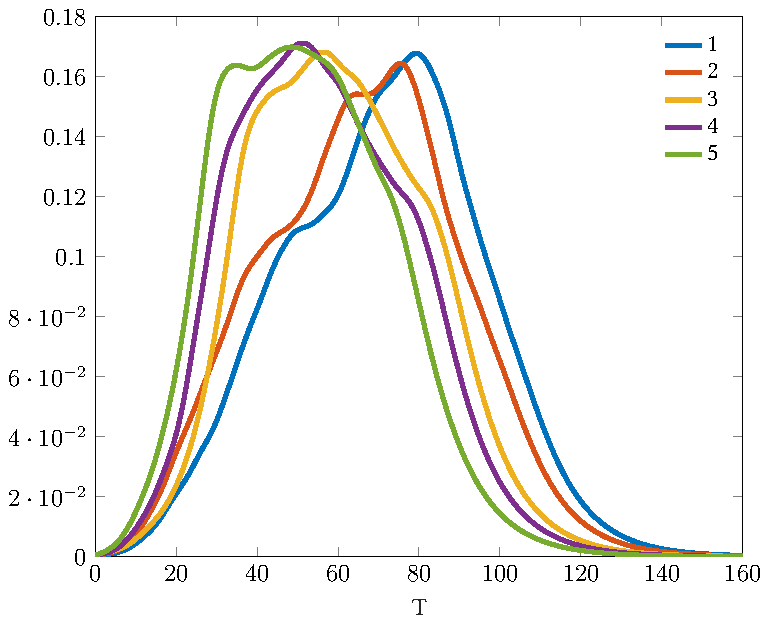
\includegraphics[scale=0.45]{Figure/minnesota_prevalenza}
\caption[Grafico della prevalenza al variare del grado del nodo inizialmente infetto.]{Grafico della prevalenza al variare del grado del nodo inizialmente infetto.\\ Per ottenere i grafici abbiamo risolto numericamente, usando MATLAB, cinque problema di Cauchy ottenuti dal modello chiuso alle coppie.\\
Per le condizioni iniziali abbiamo preso ogni volta un nodo certamente infetto (con grado diverso e tutti gli altri nodi certamente sani).\\
Per la sperimentazione abbiamo utilizzato come parametri $\tau=0.3$ e $\gamma=0.1$.}
\label{fig::minnesota_prevalenza}
\end{figure}



\bibliography{references}
\addcontentsline{toc}{chapter}{Bibliografia}
\bibliographystyle{plain}

\cleardoublepage
\listoffigures
\addcontentsline{toc}{chapter}{Elenco delle figure}
\listoftables
\addcontentsline{toc}{chapter}{Elenco delle tabelle}
\cleardoublepage
\tableofcontents

\end{document}